\documentclass[twoside]{book}

% Packages required by doxygen
\usepackage{fixltx2e}
\usepackage{calc}
\usepackage{doxygen}
\usepackage[export]{adjustbox} % also loads graphicx
\usepackage{graphicx}
\usepackage[utf8]{inputenc}
\usepackage{makeidx}
\usepackage{multicol}
\usepackage{multirow}
\PassOptionsToPackage{warn}{textcomp}
\usepackage{textcomp}
\usepackage[nointegrals]{wasysym}
\usepackage[table]{xcolor}

% Font selection
\usepackage[T1]{fontenc}
\usepackage[scaled=.90]{helvet}
\usepackage{courier}
\usepackage{amssymb}
\usepackage{sectsty}
\renewcommand{\familydefault}{\sfdefault}
\allsectionsfont{%
  \fontseries{bc}\selectfont%
  \color{darkgray}%
}
\renewcommand{\DoxyLabelFont}{%
  \fontseries{bc}\selectfont%
  \color{darkgray}%
}
\newcommand{\+}{\discretionary{\mbox{\scriptsize$\hookleftarrow$}}{}{}}

% Page & text layout
\usepackage{geometry}
\geometry{%
  a4paper,%
  top=2.5cm,%
  bottom=2.5cm,%
  left=2.5cm,%
  right=2.5cm%
}
\tolerance=750
\hfuzz=15pt
\hbadness=750
\setlength{\emergencystretch}{15pt}
\setlength{\parindent}{0cm}
\setlength{\parskip}{3ex plus 2ex minus 2ex}
\makeatletter
\renewcommand{\paragraph}{%
  \@startsection{paragraph}{4}{0ex}{-1.0ex}{1.0ex}{%
    \normalfont\normalsize\bfseries\SS@parafont%
  }%
}
\renewcommand{\subparagraph}{%
  \@startsection{subparagraph}{5}{0ex}{-1.0ex}{1.0ex}{%
    \normalfont\normalsize\bfseries\SS@subparafont%
  }%
}
\makeatother

% Headers & footers
\usepackage{fancyhdr}
\pagestyle{fancyplain}
\fancyhead[LE]{\fancyplain{}{\bfseries\thepage}}
\fancyhead[CE]{\fancyplain{}{}}
\fancyhead[RE]{\fancyplain{}{\bfseries\leftmark}}
\fancyhead[LO]{\fancyplain{}{\bfseries\rightmark}}
\fancyhead[CO]{\fancyplain{}{}}
\fancyhead[RO]{\fancyplain{}{\bfseries\thepage}}
\fancyfoot[LE]{\fancyplain{}{}}
\fancyfoot[CE]{\fancyplain{}{}}
\fancyfoot[RE]{\fancyplain{}{\bfseries\scriptsize Generated by Doxygen }}
\fancyfoot[LO]{\fancyplain{}{\bfseries\scriptsize Generated by Doxygen }}
\fancyfoot[CO]{\fancyplain{}{}}
\fancyfoot[RO]{\fancyplain{}{}}
\renewcommand{\footrulewidth}{0.4pt}
\renewcommand{\chaptermark}[1]{%
  \markboth{#1}{}%
}
\renewcommand{\sectionmark}[1]{%
  \markright{\thesection\ #1}%
}

% Indices & bibliography
\usepackage{natbib}
\usepackage[titles]{tocloft}
\setcounter{tocdepth}{3}
\setcounter{secnumdepth}{5}
\makeindex

% Hyperlinks (required, but should be loaded last)
\usepackage{ifpdf}
\ifpdf
  \usepackage[pdftex,pagebackref=true]{hyperref}
\else
  \usepackage[ps2pdf,pagebackref=true]{hyperref}
\fi
\hypersetup{%
  colorlinks=true,%
  linkcolor=blue,%
  citecolor=blue,%
  unicode%
}

% Custom commands
\newcommand{\clearemptydoublepage}{%
  \newpage{\pagestyle{empty}\cleardoublepage}%
}

\usepackage{caption}
\captionsetup{labelsep=space,justification=centering,font={bf},singlelinecheck=off,skip=4pt,position=top}

%===== C O N T E N T S =====

\begin{document}

% Titlepage & ToC
\hypersetup{pageanchor=false,
             bookmarksnumbered=true,
             pdfencoding=unicode
            }
\pagenumbering{alph}
\begin{titlepage}
\vspace*{7cm}
\begin{center}%
{\Large Le Paint }\\
\vspace*{1cm}
{\large Generated by Doxygen 1.8.14}\\
\end{center}
\end{titlepage}
\clearemptydoublepage
\pagenumbering{roman}
\tableofcontents
\clearemptydoublepage
\pagenumbering{arabic}
\hypersetup{pageanchor=true}

%--- Begin generated contents ---
\chapter{Wintab\+DN}
\label{index}\hypertarget{index}{}\mbox{\hyperlink{namespace_wintab_d_n}{Wintab\+DN}} is a wrapper of the Wintab32 A\+PI that supports writing .N\+ET compatible applications for Wacom digitizing tablets. \begin{DoxyAuthor}{Author}
Robert Cohn, Wacom Technology Corporation (\href{mailto:rcohn@wacom.com}{\tt rcohn@wacom.\+com})
\end{DoxyAuthor}
\begin{DoxyParagraph}{Revision History}
\tabulinesep=1mm
\begin{longtabu} spread 0pt [c]{*{4}{|X[-1]}|}
\hline
\rowcolor{\tableheadbgcolor}\textbf{ Revision Date}&\textbf{ Revisor\textquotesingle{}s Name (Email)}&\textbf{ Change Description}&\textbf{ Version  }\\\cline{1-4}
\endfirsthead
\hline
\endfoot
\hline
\rowcolor{\tableheadbgcolor}\textbf{ Revision Date}&\textbf{ Revisor\textquotesingle{}s Name (Email)}&\textbf{ Change Description}&\textbf{ Version  }\\\cline{1-4}
\endhead
11/13/2010&Robert Cohn (\href{mailto:rcohn@wacom.com}{\tt rcohn@wacom.\+com})&Initial Version&1.\+0  \\\cline{1-4}
03/15/2013&Robert Cohn (\href{mailto:rcohn@wacom.com}{\tt rcohn@wacom.\+com})&Added Wintab Extensions Support&1.\+1  \\\cline{1-4}
08/13/2013&Robert Cohn (\href{mailto:rcohn@wacom.com}{\tt rcohn@wacom.\+com})&Now requires .N\+ET 4; fixed Wt\+Packets\+Get testing; marshalling improvements (from \href{mailto:brett@brett.net.au}{\tt brett@brett.\+net.\+au})&1.\+2  \\\cline{1-4}
\end{longtabu}

\end{DoxyParagraph}
\hypertarget{index_intro_sec}{}\section{Introduction}\label{index_intro_sec}
The Wintab32 A\+PI (originally developed by L\+C\+S/\+Telegraphics in the early 1990s) was created to provide a standardized programming interface to digitizing tablets, and was early adopted by Wacom Technology Corporation to support writing Windows operating system native C++ applications for its pen digitizing tablets. A complete description of the Wintab32 A\+PI can be found in the \href{Wintab_v140.htm}{\tt Wintab 1.\+4 specification}.

The \mbox{\hyperlink{namespace_wintab_d_n}{Wintab\+DN}} A\+PI was created to aid the development of managed code applications for Wacom\textquotesingle{}s digital tablets. This new A\+PI is .N\+ET 2 compatible and will support the writing of applications in any .N\+ET supported language (such as C\# or V\+B.\+N\+ET).

With \mbox{\hyperlink{namespace_wintab_d_n}{Wintab\+DN}}, an application developer can, for example, easily write a .N\+ET application to set up and capture pen data indicating X/Y location and pressure. Other applications can be written to monitor pen tilt or rotation. The A\+PI can be incorporated into many software applications where precise pen location data would be useful (such as M\+A\+T\+L\+AB, or C\+AD applications).

\mbox{\hyperlink{namespace_wintab_d_n}{Wintab\+DN}} is a work in progress. Version 1.\+0 only wraps a subset of the extensive Wintab32 native implementation, and it is hoped that a growing community of developers will use \mbox{\hyperlink{namespace_wintab_d_n}{Wintab\+DN}} and contribute to its maintenance and extension.\hypertarget{index_contact_sec}{}\section{Contact Info}\label{index_contact_sec}
If you have questions about using \mbox{\hyperlink{namespace_wintab_d_n}{Wintab\+DN}}, you can send email to this address\+: \href{mailto:DeveloperEmailGroup@wacom.com}{\tt Developer\+Email\+Group@wacom.\+com}

Also, visit \href{http://wacomeng.com/windows/index.html}{\tt Wacom Software Developer Support} for general Wintab32 tablet programming support. 
\chapter{Getting Started}
\label{page1}
\Hypertarget{page1}
\hypertarget{page1_install_sec}{}\section{Installation}\label{page1_install_sec}
\hypertarget{page1_step1}{}\subsection{Step 1\+: Install the Wacom tablet driver}\label{page1_step1}
\mbox{\hyperlink{namespace_wintab_d_n}{Wintab\+DN}} communicates with the Wacom tablet via the native code Wintab32.\+dll module. This D\+LL is installed as part of the tablet driver software. It is best to get the latest tablet driver software from the Wacom driver installation site at\+: \href{http://www.wacom.com/downloads/drivers.php}{\tt http\+://www.\+wacom.\+com/downloads/drivers.\+php}.

Simply install the latest driver software for your tablet type and operating system. You may be prompted to reboot your system when the installation completes.\hypertarget{page1_step2}{}\subsection{Step 2\+: Test tablet driver installation}\label{page1_step2}
After installation, plug in your tablet and make sure you can move the mouse cursor with the tablet pen. Then, use your pen to open the table preferences dialog either from the Windows Start menu or the control panel. For example, to open the preferences dialog for a Bamboo tablet, you would select All Programs $\vert$ Bamboo $\vert$ Bamboo Preferences.

You can do a quick check to make sure that Wintab is communicating with the tablet driver before using \mbox{\hyperlink{namespace_wintab_d_n}{Wintab\+DN}}. Go to the Wacom Software Developer Support plugin site at\+: \href{http://wacomeng.com/web/index.html}{\tt http\+://wacomeng.\+com/web/index.\+html} and test one of the web plugins (for example, the Table demo). If you can see the tablet properties being updated as you move the pen around, the tablet driver software is working correctly and communicating through Wintab.

Finally, test the sample application\+: Form\+Test\+App, that comes with the \mbox{\hyperlink{namespace_wintab_d_n}{Wintab\+DN}} code distribution. Start that app and use your pen to press the \char`\"{}\+Test\char`\"{} button. You should see a stream of test output scroll down the left side of the dialog. You should also see varying pen X/\+Y/\+Pressure data as you press and lift the pen.

When you\textquotesingle{}ve had enough fun doing that, use your pen to press the \char`\"{}\+Scribble\char`\"{} button. ~\newline
Now you should be able to draw lines of varying thickness with your pen. Note that the application will not move the system cursor when operating in the Sribble mode, so you will have to use your mouse cursor (or track pad) to close the app.

The \mbox{\hyperlink{namespace_wintab_d_n}{Wintab\+DN}} distribution has full sources for this test application.\hypertarget{page1_step3}{}\subsection{Step 3\+: Building Wintab\+D\+N.\+D\+L\+L and Form\+Test\+App}\label{page1_step3}
The \mbox{\hyperlink{namespace_wintab_d_n}{Wintab\+DN}} project was built using Visual Studio 2010. Other than the tablet driver software (which includes installing the native Wintab32.\+dll), there are no other software dependencies needed to build Wintab\+D\+N.\+dll. Just press \char`\"{}\+Build\char`\"{} and you\textquotesingle{}re good to go.

The \mbox{\hyperlink{namespace_wintab_d_n}{Wintab\+DN}} solution will build both Wintab\+D\+N.\+D\+LL and the Form\+Test\+App application.\hypertarget{page1_step4}{}\subsection{Step 4\+: Building Wintab\+D\+N Documentation}\label{page1_step4}
\mbox{\hyperlink{namespace_wintab_d_n}{Wintab\+DN}} documentation is generated using the doxygen document-\/generating tool, which can be freely downloaded from\+: \href{http://www.stack.nl/~dimitri/doxygen/}{\tt http\+://www.\+stack.\+nl/$\sim$dimitri/doxygen/}.

In addition to generating H\+T\+ML web-\/help files, doxygen also uses the Windows H\+T\+ML Help tool to generate Windows compiled help (C\+HM) files. This tool can be freely downloaded from\+: \href{http://msdn.microsoft.com/en-us/library/ms669985%28VS.85%29.aspx}{\tt http\+://msdn.\+microsoft.\+com/en-\/us/library/ms669985\%28\+V\+S.\+85\%29.\+aspx}.

Document generation relies on comments within the code, as well as a doxygen configuration file. The configuration file for \mbox{\hyperlink{namespace_wintab_d_n}{Wintab\+DN}} is called, wintabdn.\+dox.

To generate documentation, execute the command\+: \begin{DoxyParagraph}{}
{\ttfamily  {\bfseries doxygen wintabdn.\+dox} } 
\end{DoxyParagraph}

\chapter{A Wintab\+DN example}
\label{page2}
\Hypertarget{page2}
The \mbox{\hyperlink{namespace_wintab_d_n}{Wintab\+DN}} distribution comes with a sample application, Form\+Test\+App, which exercises most of the \mbox{\hyperlink{namespace_wintab_d_n}{Wintab\+DN}} functionality, as well as demonstrates how to use the A\+PI to build a simple scribble application.\hypertarget{page2_scribbleDemo_sec}{}\section{Scribble Demo}\label{page2_scribbleDemo_sec}
The Scribble demo shows how to set up a context, register for Wintab data packets, provide a handler for Wintab events, and display graphics corresponding to pen X/Y position and pen pressure data.

The following code segment shows the \char`\"{}\+Scribble\char`\"{} button handler, which opens sets up for pen data capture using the {\ttfamily {\bfseries Init\+Data\+Capture()}} function. 
\begin{DoxyCode}
\textcolor{keyword}{private} \textcolor{keywordtype}{void} scribbleButton\_Click(\textcolor{keywordtype}{object} sender, EventArgs e)
\{
    ClearDisplay();
    CloseCurrentContext();
    Enable\_Scribble(\textcolor{keyword}{true});

    \textcolor{comment}{// Open a context and try to capture pen data;}
    \textcolor{comment}{// Do not control system cursor.}

    InitDataCapture(m\_TABEXTX, m\_TABEXTY, \textcolor{keyword}{false});
\}
\end{DoxyCode}


{\ttfamily {\bfseries Init\+Data\+Capture()}} makes sure it closes the current Wintab context, opens up a new context with {\ttfamily {\bfseries Open\+Test\+Digitizer\+Context()}}, creates a Wintab data object with {\ttfamily {\bfseries new C\+Wintab\+Data(m\+\_\+log\+Context)}}, which uses the context just created, and finally sets up a packet event handler for being notified when pen data comes in. Note that the call to {\ttfamily {\bfseries Init\+Data\+Capture()}} is made with ctrl\+Sys\+Cursor\+\_\+I = false, because we cannot be controlling the system cursor while scribbling.


\begin{DoxyCode}
\textcolor{keyword}{private} \textcolor{keywordtype}{void} InitDataCapture(
\textcolor{keywordtype}{int} ctxHeight\_I = m\_TABEXTX, \textcolor{keywordtype}{int} ctxWidth\_I = m\_TABEXTY, \textcolor{keywordtype}{bool} ctrlSysCursor\_I = \textcolor{keyword}{true})
\{
    \textcolor{keywordflow}{try}
    \{
        \textcolor{comment}{// Close context from any previous test.}
        CloseCurrentContext();

        m\_logContext = OpenTestDigitizerContext(ctxWidth\_I, ctxHeight\_I,  ctrlSysCursor\_I);

        \textcolor{keywordflow}{if} (m\_logContext == null)
        \{
            \textcolor{keywordflow}{return};
        \}

        \textcolor{comment}{// Create a data object and set its WT\_PACKET handler.}
        m\_wtData = \textcolor{keyword}{new} CWintabData(m\_logContext);
        m\_wtData.SetWTPacketEventHandler(MyWTPacketEventHandler);
    \}
    \textcolor{keywordflow}{catch} (Exception ex)
    \{
        MessageBox.Show(ex.ToString());
    \}
\}
\end{DoxyCode}


When creating the digitizer context, we start with getting the default context using {\ttfamily {\bfseries C\+Wintab\+Info.\+Get\+Default\+Digitizing\+Context(E\+C\+T\+X\+Option\+Values.\+C\+X\+O\+\_\+\+M\+E\+S\+S\+A\+G\+ES)}}, which specifies that we want to receive Wintab messages to be notified of pen data. Since we are not specifying that we want to control the system cursor, the only other thing we have to override is the description of the logical extent of the tablet coordinates. For this example, we specify a logical tablet size of 10000 x 10000. That\textquotesingle{}s pretty much it. We just tell \mbox{\hyperlink{namespace_wintab_d_n}{Wintab\+DN}} to open this context using {\ttfamily {\bfseries log\+Context.\+Open()}}.


\begin{DoxyCode}
\textcolor{keyword}{private} CWintabContext OpenTestDigitizerContext(
    \textcolor{keywordtype}{int} width\_I = m\_TABEXTX, \textcolor{keywordtype}{int} height\_I = m\_TABEXTY, \textcolor{keywordtype}{bool} ctrlSysCursor = \textcolor{keyword}{true})
\{
    \textcolor{keywordtype}{bool} status = \textcolor{keyword}{false};
    CWintabContext logContext = null;

    \textcolor{keywordflow}{try}
    \{
        \textcolor{comment}{// Get the default digitizing context.}
        \textcolor{comment}{// Default is to receive data events.}
        logContext = CWintabInfo.GetDefaultDigitizingContext(\mbox{\hyperlink{namespace_wintab_d_n_a701e8021b6889039ed562596a2d1bdd2}{ECTXOptionValues}}.CXO\_MESSAGES)
      ;

        \textcolor{comment}{// Set system cursor if caller wants it.}
        \textcolor{keywordflow}{if} (ctrlSysCursor)
        \{
            logContext.Options |= (uint)\mbox{\hyperlink{namespace_wintab_d_n_a701e8021b6889039ed562596a2d1bdd2}{ECTXOptionValues}}.CXO\_SYSTEM;
        \}

        \textcolor{keywordflow}{if} (logContext == null)
        \{
            \textcolor{keywordflow}{return} null;
        \}

        \textcolor{comment}{// Modify the digitizing region.}
        logContext.Name = \textcolor{stringliteral}{"WintabDN Event Data Context"};

        \textcolor{comment}{// output in a 10000 x 10000 grid}
        logContext.OutOrgX = logContext.OutOrgY = 0;
        logContext.OutExtX = width\_I;
        logContext.OutExtY = height\_I;


        \textcolor{comment}{// Open the context, which will also tell Wintab to send data packets.}
        status = logContext.Open();
    \}
    \textcolor{keywordflow}{catch} (Exception ex)
    \{
        TraceMsg(\textcolor{stringliteral}{"OpenTestDigitizerContext ERROR: "} + ex.ToString());
    \}

    \textcolor{keywordflow}{return} logContext;
\}
\end{DoxyCode}


Finally, we show that the event handler can easily access the pen data using {\ttfamily {\bfseries m\+\_\+wt\+Data.\+Get\+Data\+Packet(pkt\+I\+D)}}. The packet contains values for the X/Y position and pen normal pressure. The example also makes use of the packet timestamp, which helps determine whether to draw a line between points or just draw a rectangle at the point. This allows the drawn lines to be less choppy when the user moves the pen quickly.


\begin{DoxyCode}
\textcolor{keyword}{public} \textcolor{keywordtype}{void} MyWTPacketEventHandler(Object sender\_I, MessageReceivedEventArgs eventArgs\_I)
\{
    \textcolor{keywordflow}{try}
    \{
        \textcolor{keywordflow}{if} (m\_maxPkts == 1)
        \{
            uint pktID = (uint)eventArgs\_I.Message.WParam;
            WintabPacket pkt = m\_wtData.GetDataPacket(pktID);

            \textcolor{keywordflow}{if} (pkt.pkContext != 0)
            \{
                m\_pkX = pkt.pkX;
                m\_pkY = pkt.pkY;
                m\_pressure = pkt.pkNormalPressure.pkAbsoluteNormalPressure;

                m\_pkTime = pkt.pkTime;

                \textcolor{keywordflow}{if} (m\_graphics != null)
                \{
                    \textcolor{comment}{// scribble mode}
                    \textcolor{keywordtype}{int} clientWidth = scribblePanel.Width;
                    \textcolor{keywordtype}{int} clientHeight = scribblePanel.Height;

                    \textcolor{keywordtype}{int} X = (int)((\textcolor{keywordtype}{double})(m\_pkX * clientWidth) / (\textcolor{keywordtype}{double})m\_TABEXTX);
                    \textcolor{keywordtype}{int} Y = (int)((\textcolor{keywordtype}{double})clientHeight - 
                        ((double)(m\_pkY * clientHeight) / (double)m\_TABEXTY));

                    Point tabPoint = \textcolor{keyword}{new} Point(X, Y);

                    \textcolor{keywordflow}{if} (m\_lastPoint.Equals(Point.Empty))
                    \{
                        m\_lastPoint = tabPoint;
                        m\_pkTimeLast = m\_pkTime;
                    \}

                    m\_pen.Width = (float)(m\_pressure / 200);
                    \textcolor{keywordflow}{if} (m\_pressure > 0)
                    \{
                        \textcolor{keywordflow}{if} (m\_pkTime - m\_pkTimeLast < 5)
                        \{
                            m\_graphics.DrawRectangle(m\_pen, X, Y, 1, 1);
                        \}
                        \textcolor{keywordflow}{else}
                        \{
                            m\_graphics.DrawLine(m\_pen, tabPoint, m\_lastPoint);
                        \}
                    \}

                    m\_lastPoint = tabPoint;
                    m\_pkTimeLast = m\_pkTime;
                \}
            \}
        \}
    \}
    \textcolor{keywordflow}{catch} (Exception ex)
    \{
        \textcolor{keywordflow}{throw} \textcolor{keyword}{new} Exception(\textcolor{stringliteral}{"FAILED to get packet data: "} + ex.ToString());
    \}
\}
\end{DoxyCode}
\hypertarget{page2_testWTInfo_sec}{}\section{Testing C\+Wintab\+Info}\label{page2_testWTInfo_sec}
The testing in this section is just a demonstration of the various C\+Wintab\+D\+N.\+C\+Wintab\+Info properties. ~\newline
 Here is one of the first calls an application might make to determine if Wintab is properly connected on the system\+: 
\begin{DoxyCode}
\textcolor{keywordtype}{bool} isWintabAvailable = CWintabInfo.IsWintabAvailable();
\end{DoxyCode}


This is an example of how to find the number of tablet devices connected\+: 
\begin{DoxyCode}
UInt32 numDevices = CWintabInfo.GetNumberOfDevices();
\end{DoxyCode}


Here is an example of how easy it is to get a default digitizing context (which is used in the \mbox{\hyperlink{page2_scribbleDemo_sec}{Scribble Demo}} example)\+: 
\begin{DoxyCode}
CWintabContext context = CWintabInfo.GetDefaultDigitizingContext();
\end{DoxyCode}


You can look through the other tests to see how some of the other global Wintab properties can be accessed.

One of the tests, {\ttfamily {\bfseries Test\+\_\+\+Get\+Data\+Packets()}} gives a demonstration of capturing data packets and writing them out to the list. This demo is very similar to the \mbox{\hyperlink{page2_scribbleDemo_sec}{Scribble Demo}}, so we won\textquotesingle{}t go into much detail here except to note that the call to {\ttfamily {\bfseries Init\+Data\+Capture()}} is made with {\ttfamily {\bfseries ctrl\+Sys\+Cursor\+\_\+I}} being true, so that the system cursor can be controlled with the pen. 
\chapter{Primary Wintab\+DN Classes}
\label{page3}
\Hypertarget{page3}
\hypertarget{page3_cwintabinfo_sec}{}\section{C\+Wintab\+Info}\label{page3_cwintabinfo_sec}
This section describes the class \mbox{\hyperlink{class_wintab_d_n_1_1_c_wintab_info}{Wintab\+D\+N.\+C\+Wintab\+Info}}, which may be used to query and set global attributes for the connected tablet. Such attributes include\+: tablet coordinates, physical dimensions, capabilities, and cursor types.\hypertarget{page3_cwintabcontext_sec}{}\section{C\+Wintab\+Context}\label{page3_cwintabcontext_sec}
This section describes the class \mbox{\hyperlink{class_wintab_d_n_1_1_c_wintab_context}{Wintab\+D\+N.\+C\+Wintab\+Context}}, which may be used when opening and manipulating Wintab contexts. This class contains everything applications and tablet managers need to know about a context. To simplify context manipulations, applications may want to take advantage of the default digitizing context available via \mbox{\hyperlink{class_wintab_d_n_1_1_c_wintab_info_a7bceb028e21a4c94d44ba0e3b8a75fa4}{Wintab\+D\+N.\+C\+Wintab\+Info.\+Get\+Default\+Digitizing\+Context()}}.\hypertarget{page3_cwintabdata_sec}{}\section{C\+Wintab\+Data}\label{page3_cwintabdata_sec}
This section describes the class \mbox{\hyperlink{class_wintab_d_n_1_1_c_wintab_data}{Wintab\+D\+N.\+C\+Wintab\+Data}}, which may be used to capture pen data from the target digitizing tablet. Such data includes pen X/Y location, pen pressure, time stamp, and much more. See \mbox{\hyperlink{struct_wintab_d_n_1_1_wintab_packet}{Wintab\+D\+N.\+Wintab\+Packet}} for a complete list of all supported pen tablet data. 
\chapter{Namespace Index}
\section{Namespace List}
Here is a list of all namespaces with brief descriptions\+:\begin{DoxyCompactList}
\item\contentsline{section}{\mbox{\hyperlink{namespace_paint___program}{Paint\+\_\+\+Program}} }{\pageref{namespace_paint___program}}{}
\item\contentsline{section}{\mbox{\hyperlink{namespace_wintab_d_n}{Wintab\+DN}} }{\pageref{namespace_wintab_d_n}}{}
\end{DoxyCompactList}

\chapter{Hierarchical Index}
\section{Class Hierarchy}
This inheritance list is sorted roughly, but not completely, alphabetically\+:\begin{DoxyCompactList}
\item \contentsline{section}{Wintab\+D\+N.\+C\+Mem\+Utils}{\pageref{class_wintab_d_n_1_1_c_mem_utils}}{}
\item \contentsline{section}{Wintab\+D\+N.\+C\+Wintab\+Context}{\pageref{class_wintab_d_n_1_1_c_wintab_context}}{}
\item \contentsline{section}{Wintab\+D\+N.\+C\+Wintab\+Data}{\pageref{class_wintab_d_n_1_1_c_wintab_data}}{}
\item \contentsline{section}{Wintab\+D\+N.\+C\+Wintab\+Extensions}{\pageref{class_wintab_d_n_1_1_c_wintab_extensions}}{}
\item \contentsline{section}{Wintab\+D\+N.\+C\+Wintab\+Funcs}{\pageref{class_wintab_d_n_1_1_c_wintab_funcs}}{}
\item \contentsline{section}{Wintab\+D\+N.\+C\+Wintab\+Info}{\pageref{class_wintab_d_n_1_1_c_wintab_info}}{}
\item \contentsline{section}{Paint\+\_\+\+Program.\+Debug\+Tool}{\pageref{class_paint___program_1_1_debug_tool}}{}
\item Event\+Args\begin{DoxyCompactList}
\item \contentsline{section}{Wintab\+D\+N.\+Message\+Received\+Event\+Args}{\pageref{class_wintab_d_n_1_1_message_received_event_args}}{}
\end{DoxyCompactList}
\item \contentsline{section}{Paint\+\_\+\+Program.\+File\+Save}{\pageref{class_paint___program_1_1_file_save}}{}
\item \contentsline{section}{Wintab\+D\+N.\+F\+I\+X32}{\pageref{class_wintab_d_n_1_1_f_i_x32}}{}
\item Form\begin{DoxyCompactList}
\item \contentsline{section}{Paint\+\_\+\+Program.\+Form1}{\pageref{class_paint___program_1_1_form1}}{}
\item \contentsline{section}{Paint\+\_\+\+Program.\+G\+Drive\+Save\+Dialog}{\pageref{class_paint___program_1_1_g_drive_save_dialog}}{}
\item \contentsline{section}{Paint\+\_\+\+Program.\+New\+Project\+Form}{\pageref{class_paint___program_1_1_new_project_form}}{}
\item \contentsline{section}{Paint\+\_\+\+Program.\+Text\+Select}{\pageref{class_paint___program_1_1_text_select}}{}
\item \contentsline{section}{Wintab\+D\+N.\+Message\+Events.\+Message\+Window}{\pageref{class_wintab_d_n_1_1_message_events_1_1_message_window}}{}
\end{DoxyCompactList}
\item \contentsline{section}{Paint\+\_\+\+Program.\+Google\+Drive\+Upload}{\pageref{class_paint___program_1_1_google_drive_upload}}{}
\item \contentsline{section}{Wintab\+D\+N.\+H\+C\+TX}{\pageref{class_wintab_d_n_1_1_h_c_t_x}}{}
\item \contentsline{section}{Wintab\+D\+N.\+H\+W\+ND}{\pageref{struct_wintab_d_n_1_1_h_w_n_d}}{}
\item I\+Disposable\begin{DoxyCompactList}
\item \contentsline{section}{Paint\+\_\+\+Program.\+Gif\+Encoder}{\pageref{class_paint___program_1_1_gif_encoder}}{}
\end{DoxyCompactList}
\item \contentsline{section}{Paint\+\_\+\+Program.\+Image\+Import}{\pageref{class_paint___program_1_1_image_import}}{}
\item \contentsline{section}{Paint\+\_\+\+Program.\+I\+Text\+Update}{\pageref{interface_paint___program_1_1_i_text_update}}{}
\begin{DoxyCompactList}
\item \contentsline{section}{Paint\+\_\+\+Program.\+Brush\+Settings}{\pageref{class_paint___program_1_1_brush_settings}}{}
\item \contentsline{section}{Paint\+\_\+\+Program.\+Canvas}{\pageref{class_paint___program_1_1_canvas}}{}
\item \contentsline{section}{Paint\+\_\+\+Program.\+Layer\+Item}{\pageref{class_paint___program_1_1_layer_item}}{}
\item \contentsline{section}{Paint\+\_\+\+Program.\+Layer\+View}{\pageref{class_paint___program_1_1_layer_view}}{}
\item \contentsline{section}{Paint\+\_\+\+Program.\+Zoom\+Control}{\pageref{class_paint___program_1_1_zoom_control}}{}
\end{DoxyCompactList}
\item \contentsline{section}{Paint\+\_\+\+Program.\+I\+Tool}{\pageref{interface_paint___program_1_1_i_tool}}{}
\begin{DoxyCompactList}
\item \contentsline{section}{Paint\+\_\+\+Program.\+Brush\+Tool}{\pageref{class_paint___program_1_1_brush_tool}}{}
\item \contentsline{section}{Paint\+\_\+\+Program.\+Color\+Sampling\+Tool}{\pageref{class_paint___program_1_1_color_sampling_tool}}{}
\item \contentsline{section}{Paint\+\_\+\+Program.\+Eraser\+Tool}{\pageref{class_paint___program_1_1_eraser_tool}}{}
\item \contentsline{section}{Paint\+\_\+\+Program.\+Green\+Screen\+Tool}{\pageref{class_paint___program_1_1_green_screen_tool}}{}
\item \contentsline{section}{Paint\+\_\+\+Program.\+Move\+Tool}{\pageref{class_paint___program_1_1_move_tool}}{}
\item \contentsline{section}{Paint\+\_\+\+Program.\+Paint\+Bucket\+Tool}{\pageref{class_paint___program_1_1_paint_bucket_tool}}{}
\item \contentsline{section}{Paint\+\_\+\+Program.\+Pencil\+Tool}{\pageref{class_paint___program_1_1_pencil_tool}}{}
\item \contentsline{section}{Paint\+\_\+\+Program.\+Selection\+Tool}{\pageref{class_paint___program_1_1_selection_tool}}{}
\item \contentsline{section}{Paint\+\_\+\+Program.\+Straight\+Line\+Tool}{\pageref{class_paint___program_1_1_straight_line_tool}}{}
\item \contentsline{section}{Paint\+\_\+\+Program.\+Text\+Tool}{\pageref{class_paint___program_1_1_text_tool}}{}
\end{DoxyCompactList}
\item \contentsline{section}{Wintab\+D\+N.\+Message\+Events}{\pageref{class_wintab_d_n_1_1_message_events}}{}
\item Panel\begin{DoxyCompactList}
\item \contentsline{section}{Paint\+\_\+\+Program.\+Display}{\pageref{class_paint___program_1_1_display}}{}
\end{DoxyCompactList}
\item \contentsline{section}{Paint\+\_\+\+Program.\+Program}{\pageref{class_paint___program_1_1_program}}{}
\item \contentsline{section}{Paint\+\_\+\+Program.\+Project\+Load}{\pageref{class_paint___program_1_1_project_load}}{}
\item \contentsline{section}{Paint\+\_\+\+Program.\+Project\+Save}{\pageref{class_paint___program_1_1_project_save}}{}
\item \contentsline{section}{Paint\+\_\+\+Program.\+Save\+To\+Drive}{\pageref{class_paint___program_1_1_save_to_drive}}{}
\item \contentsline{section}{Paint\+\_\+\+Program.\+Shared\+Settings}{\pageref{class_paint___program_1_1_shared_settings}}{}
\item \contentsline{section}{Paint\+\_\+\+Program.\+Tablet\+Info}{\pageref{class_paint___program_1_1_tablet_info}}{}
\item User\+Control\begin{DoxyCompactList}
\item \contentsline{section}{Paint\+\_\+\+Program.\+Brush\+Settings}{\pageref{class_paint___program_1_1_brush_settings}}{}
\item \contentsline{section}{Paint\+\_\+\+Program.\+Canvas}{\pageref{class_paint___program_1_1_canvas}}{}
\item \contentsline{section}{Paint\+\_\+\+Program.\+Layer\+Item}{\pageref{class_paint___program_1_1_layer_item}}{}
\item \contentsline{section}{Paint\+\_\+\+Program.\+Layer\+View}{\pageref{class_paint___program_1_1_layer_view}}{}
\item \contentsline{section}{Paint\+\_\+\+Program.\+Zoom\+Control}{\pageref{class_paint___program_1_1_zoom_control}}{}
\end{DoxyCompactList}
\item \contentsline{section}{Wintab\+D\+N.\+Wintab\+Axis}{\pageref{struct_wintab_d_n_1_1_wintab_axis}}{}
\item \contentsline{section}{Wintab\+D\+N.\+Wintab\+Axis\+Array}{\pageref{struct_wintab_d_n_1_1_wintab_axis_array}}{}
\item \contentsline{section}{Wintab\+D\+N.\+Wintab\+Log\+Context}{\pageref{struct_wintab_d_n_1_1_wintab_log_context}}{}
\item \contentsline{section}{Wintab\+D\+N.\+Wintab\+Packet}{\pageref{struct_wintab_d_n_1_1_wintab_packet}}{}
\item \contentsline{section}{Wintab\+D\+N.\+Wintab\+Packet\+Ext}{\pageref{struct_wintab_d_n_1_1_wintab_packet_ext}}{}
\item \contentsline{section}{Wintab\+D\+N.\+W\+T\+Exp\+Key\+Data}{\pageref{struct_wintab_d_n_1_1_w_t_exp_key_data}}{}
\item \contentsline{section}{Wintab\+D\+N.\+W\+T\+Extension\+Base}{\pageref{struct_wintab_d_n_1_1_w_t_extension_base}}{}
\item \contentsline{section}{Wintab\+D\+N.\+W\+T\+Extension\+Image\+Property}{\pageref{struct_wintab_d_n_1_1_w_t_extension_image_property}}{}
\item \contentsline{section}{Wintab\+D\+N.\+W\+T\+Extension\+Property}{\pageref{struct_wintab_d_n_1_1_w_t_extension_property}}{}
\item \contentsline{section}{Wintab\+D\+N.\+W\+T\+Extension\+Property\+Base}{\pageref{struct_wintab_d_n_1_1_w_t_extension_property_base}}{}
\item \contentsline{section}{Wintab\+D\+N.\+W\+T\+Extensions\+Global}{\pageref{class_wintab_d_n_1_1_w_t_extensions_global}}{}
\item \contentsline{section}{Wintab\+D\+N.\+W\+T\+Orientation}{\pageref{struct_wintab_d_n_1_1_w_t_orientation}}{}
\item \contentsline{section}{Wintab\+D\+N.\+W\+T\+P\+KT}{\pageref{class_wintab_d_n_1_1_w_t_p_k_t}}{}
\item \contentsline{section}{Wintab\+D\+N.\+W\+T\+Rotation}{\pageref{struct_wintab_d_n_1_1_w_t_rotation}}{}
\item \contentsline{section}{Wintab\+D\+N.\+W\+T\+Slider\+Data}{\pageref{struct_wintab_d_n_1_1_w_t_slider_data}}{}
\end{DoxyCompactList}

\chapter{Class Index}
\section{Class List}
Here are the classes, structs, unions and interfaces with brief descriptions\+:\begin{DoxyCompactList}
\item\contentsline{section}{\mbox{\hyperlink{class_paint___program_1_1_brush_settings}{Paint\+\_\+\+Program.\+Brush\+Settings}} }{\pageref{class_paint___program_1_1_brush_settings}}{}
\item\contentsline{section}{\mbox{\hyperlink{class_paint___program_1_1_brush_tool}{Paint\+\_\+\+Program.\+Brush\+Tool}} }{\pageref{class_paint___program_1_1_brush_tool}}{}
\item\contentsline{section}{\mbox{\hyperlink{class_paint___program_1_1_canvas}{Paint\+\_\+\+Program.\+Canvas}} \\*Class handling the main rendering of the layers, and interfacing with tools }{\pageref{class_paint___program_1_1_canvas}}{}
\item\contentsline{section}{\mbox{\hyperlink{class_wintab_d_n_1_1_c_mem_utils}{Wintab\+D\+N.\+C\+Mem\+Utils}} \\*Provide utility methods for unmanaged memory management. }{\pageref{class_wintab_d_n_1_1_c_mem_utils}}{}
\item\contentsline{section}{\mbox{\hyperlink{class_paint___program_1_1_color_sampling_tool}{Paint\+\_\+\+Program.\+Color\+Sampling\+Tool}} }{\pageref{class_paint___program_1_1_color_sampling_tool}}{}
\item\contentsline{section}{\mbox{\hyperlink{class_wintab_d_n_1_1_c_wintab_context}{Wintab\+D\+N.\+C\+Wintab\+Context}} \\*Class to support access to Wintab context management. }{\pageref{class_wintab_d_n_1_1_c_wintab_context}}{}
\item\contentsline{section}{\mbox{\hyperlink{class_wintab_d_n_1_1_c_wintab_data}{Wintab\+D\+N.\+C\+Wintab\+Data}} \\*Class to support capture and management of Wintab daa. }{\pageref{class_wintab_d_n_1_1_c_wintab_data}}{}
\item\contentsline{section}{\mbox{\hyperlink{class_wintab_d_n_1_1_c_wintab_extensions}{Wintab\+D\+N.\+C\+Wintab\+Extensions}} \\*A\+PI for Wintab extensions functionality (Wintab 1.\+4) }{\pageref{class_wintab_d_n_1_1_c_wintab_extensions}}{}
\item\contentsline{section}{\mbox{\hyperlink{class_wintab_d_n_1_1_c_wintab_funcs}{Wintab\+D\+N.\+C\+Wintab\+Funcs}} \\*P/\+Invoke wrappers for Wintab functions. See Wintab\+\_\+v140.\+doc (Wintab 1.\+4 spec) and related Wintab documentation for details. }{\pageref{class_wintab_d_n_1_1_c_wintab_funcs}}{}
\item\contentsline{section}{\mbox{\hyperlink{class_wintab_d_n_1_1_c_wintab_info}{Wintab\+D\+N.\+C\+Wintab\+Info}} \\*Class to access Wintab interface data. }{\pageref{class_wintab_d_n_1_1_c_wintab_info}}{}
\item\contentsline{section}{\mbox{\hyperlink{class_paint___program_1_1_debug_tool}{Paint\+\_\+\+Program.\+Debug\+Tool}} \\*Debug class, please ignore }{\pageref{class_paint___program_1_1_debug_tool}}{}
\item\contentsline{section}{\mbox{\hyperlink{class_paint___program_1_1_display}{Paint\+\_\+\+Program.\+Display}} }{\pageref{class_paint___program_1_1_display}}{}
\item\contentsline{section}{\mbox{\hyperlink{class_paint___program_1_1_eraser_tool}{Paint\+\_\+\+Program.\+Eraser\+Tool}} }{\pageref{class_paint___program_1_1_eraser_tool}}{}
\item\contentsline{section}{\mbox{\hyperlink{class_paint___program_1_1_file_save}{Paint\+\_\+\+Program.\+File\+Save}} }{\pageref{class_paint___program_1_1_file_save}}{}
\item\contentsline{section}{\mbox{\hyperlink{class_wintab_d_n_1_1_f_i_x32}{Wintab\+D\+N.\+F\+I\+X32}} \\*Managed implementation of Wintab \mbox{\hyperlink{class_wintab_d_n_1_1_f_i_x32}{F\+I\+X32}} typedef. Used for a fixed-\/point arithmetic value. }{\pageref{class_wintab_d_n_1_1_f_i_x32}}{}
\item\contentsline{section}{\mbox{\hyperlink{class_paint___program_1_1_form1}{Paint\+\_\+\+Program.\+Form1}} }{\pageref{class_paint___program_1_1_form1}}{}
\item\contentsline{section}{\mbox{\hyperlink{class_paint___program_1_1_g_drive_save_dialog}{Paint\+\_\+\+Program.\+G\+Drive\+Save\+Dialog}} }{\pageref{class_paint___program_1_1_g_drive_save_dialog}}{}
\item\contentsline{section}{\mbox{\hyperlink{class_paint___program_1_1_gif_encoder}{Paint\+\_\+\+Program.\+Gif\+Encoder}} \\*Encodes multiple images as an animated gif to a stream. ~\newline
 A\+L\+W\+A\+YS A\+L\+W\+A\+YS A\+L\+W\+A\+YS wire this up in a using block ~\newline
 Disposing the encoder will complete the file. ~\newline
 Uses default .net G\+IF encoding and adds animation headers. }{\pageref{class_paint___program_1_1_gif_encoder}}{}
\item\contentsline{section}{\mbox{\hyperlink{class_paint___program_1_1_google_drive_upload}{Paint\+\_\+\+Program.\+Google\+Drive\+Upload}} }{\pageref{class_paint___program_1_1_google_drive_upload}}{}
\item\contentsline{section}{\mbox{\hyperlink{class_paint___program_1_1_green_screen_tool}{Paint\+\_\+\+Program.\+Green\+Screen\+Tool}} }{\pageref{class_paint___program_1_1_green_screen_tool}}{}
\item\contentsline{section}{\mbox{\hyperlink{class_wintab_d_n_1_1_h_c_t_x}{Wintab\+D\+N.\+H\+C\+TX}} \\*Managed implementation of Wintab \mbox{\hyperlink{class_wintab_d_n_1_1_h_c_t_x}{H\+C\+TX}} typedef. Holds a Wintab context identifier. }{\pageref{class_wintab_d_n_1_1_h_c_t_x}}{}
\item\contentsline{section}{\mbox{\hyperlink{struct_wintab_d_n_1_1_h_w_n_d}{Wintab\+D\+N.\+H\+W\+ND}} \\*Managed implementation of Wintab \mbox{\hyperlink{struct_wintab_d_n_1_1_h_w_n_d}{H\+W\+ND}} typedef. Holds native Window handle. }{\pageref{struct_wintab_d_n_1_1_h_w_n_d}}{}
\item\contentsline{section}{\mbox{\hyperlink{class_paint___program_1_1_image_import}{Paint\+\_\+\+Program.\+Image\+Import}} }{\pageref{class_paint___program_1_1_image_import}}{}
\item\contentsline{section}{\mbox{\hyperlink{interface_paint___program_1_1_i_text_update}{Paint\+\_\+\+Program.\+I\+Text\+Update}} }{\pageref{interface_paint___program_1_1_i_text_update}}{}
\item\contentsline{section}{\mbox{\hyperlink{interface_paint___program_1_1_i_tool}{Paint\+\_\+\+Program.\+I\+Tool}} }{\pageref{interface_paint___program_1_1_i_tool}}{}
\item\contentsline{section}{\mbox{\hyperlink{class_paint___program_1_1_layer_item}{Paint\+\_\+\+Program.\+Layer\+Item}} }{\pageref{class_paint___program_1_1_layer_item}}{}
\item\contentsline{section}{\mbox{\hyperlink{class_paint___program_1_1_layer_view}{Paint\+\_\+\+Program.\+Layer\+View}} }{\pageref{class_paint___program_1_1_layer_view}}{}
\item\contentsline{section}{\mbox{\hyperlink{class_wintab_d_n_1_1_message_events}{Wintab\+D\+N.\+Message\+Events}} \\*Windows native message handler, to provide support for detecting and responding to Wintab messages. }{\pageref{class_wintab_d_n_1_1_message_events}}{}
\item\contentsline{section}{\mbox{\hyperlink{class_wintab_d_n_1_1_message_received_event_args}{Wintab\+D\+N.\+Message\+Received\+Event\+Args}} \\*Support for registering a Native Windows message with \mbox{\hyperlink{class_wintab_d_n_1_1_message_events}{Message\+Events}} class. }{\pageref{class_wintab_d_n_1_1_message_received_event_args}}{}
\item\contentsline{section}{\mbox{\hyperlink{class_wintab_d_n_1_1_message_events_1_1_message_window}{Wintab\+D\+N.\+Message\+Events.\+Message\+Window}} }{\pageref{class_wintab_d_n_1_1_message_events_1_1_message_window}}{}
\item\contentsline{section}{\mbox{\hyperlink{class_paint___program_1_1_move_tool}{Paint\+\_\+\+Program.\+Move\+Tool}} }{\pageref{class_paint___program_1_1_move_tool}}{}
\item\contentsline{section}{\mbox{\hyperlink{class_paint___program_1_1_new_project_form}{Paint\+\_\+\+Program.\+New\+Project\+Form}} }{\pageref{class_paint___program_1_1_new_project_form}}{}
\item\contentsline{section}{\mbox{\hyperlink{class_paint___program_1_1_paint_bucket_tool}{Paint\+\_\+\+Program.\+Paint\+Bucket\+Tool}} }{\pageref{class_paint___program_1_1_paint_bucket_tool}}{}
\item\contentsline{section}{\mbox{\hyperlink{class_paint___program_1_1_pencil_tool}{Paint\+\_\+\+Program.\+Pencil\+Tool}} }{\pageref{class_paint___program_1_1_pencil_tool}}{}
\item\contentsline{section}{\mbox{\hyperlink{class_paint___program_1_1_program}{Paint\+\_\+\+Program.\+Program}} }{\pageref{class_paint___program_1_1_program}}{}
\item\contentsline{section}{\mbox{\hyperlink{class_paint___program_1_1_project_load}{Paint\+\_\+\+Program.\+Project\+Load}} }{\pageref{class_paint___program_1_1_project_load}}{}
\item\contentsline{section}{\mbox{\hyperlink{class_paint___program_1_1_project_save}{Paint\+\_\+\+Program.\+Project\+Save}} }{\pageref{class_paint___program_1_1_project_save}}{}
\item\contentsline{section}{\mbox{\hyperlink{class_paint___program_1_1_save_to_drive}{Paint\+\_\+\+Program.\+Save\+To\+Drive}} }{\pageref{class_paint___program_1_1_save_to_drive}}{}
\item\contentsline{section}{\mbox{\hyperlink{class_paint___program_1_1_selection_tool}{Paint\+\_\+\+Program.\+Selection\+Tool}} }{\pageref{class_paint___program_1_1_selection_tool}}{}
\item\contentsline{section}{\mbox{\hyperlink{class_paint___program_1_1_shared_settings}{Paint\+\_\+\+Program.\+Shared\+Settings}} }{\pageref{class_paint___program_1_1_shared_settings}}{}
\item\contentsline{section}{\mbox{\hyperlink{class_paint___program_1_1_straight_line_tool}{Paint\+\_\+\+Program.\+Straight\+Line\+Tool}} }{\pageref{class_paint___program_1_1_straight_line_tool}}{}
\item\contentsline{section}{\mbox{\hyperlink{class_paint___program_1_1_tablet_info}{Paint\+\_\+\+Program.\+Tablet\+Info}} }{\pageref{class_paint___program_1_1_tablet_info}}{}
\item\contentsline{section}{\mbox{\hyperlink{class_paint___program_1_1_text_select}{Paint\+\_\+\+Program.\+Text\+Select}} }{\pageref{class_paint___program_1_1_text_select}}{}
\item\contentsline{section}{\mbox{\hyperlink{class_paint___program_1_1_text_tool}{Paint\+\_\+\+Program.\+Text\+Tool}} }{\pageref{class_paint___program_1_1_text_tool}}{}
\item\contentsline{section}{\mbox{\hyperlink{struct_wintab_d_n_1_1_wintab_axis}{Wintab\+D\+N.\+Wintab\+Axis}} \\*Managed version of A\+X\+IS struct. }{\pageref{struct_wintab_d_n_1_1_wintab_axis}}{}
\item\contentsline{section}{\mbox{\hyperlink{struct_wintab_d_n_1_1_wintab_axis_array}{Wintab\+D\+N.\+Wintab\+Axis\+Array}} \\*Array of \mbox{\hyperlink{struct_wintab_d_n_1_1_wintab_axis}{Wintab\+Axis}} objects. }{\pageref{struct_wintab_d_n_1_1_wintab_axis_array}}{}
\item\contentsline{section}{\mbox{\hyperlink{struct_wintab_d_n_1_1_wintab_log_context}{Wintab\+D\+N.\+Wintab\+Log\+Context}} \\*Managed version of Wintab L\+O\+G\+C\+O\+N\+T\+E\+XT struct. This structure determines what events an application will get, how they will be processed, and how they will be delivered to the application or to Windows itself. }{\pageref{struct_wintab_d_n_1_1_wintab_log_context}}{}
\item\contentsline{section}{\mbox{\hyperlink{struct_wintab_d_n_1_1_wintab_packet}{Wintab\+D\+N.\+Wintab\+Packet}} \\*Wintab data packet. Contains the \char`\"{}\+Full Monty\char`\"{} for all possible data values. }{\pageref{struct_wintab_d_n_1_1_wintab_packet}}{}
\item\contentsline{section}{\mbox{\hyperlink{struct_wintab_d_n_1_1_wintab_packet_ext}{Wintab\+D\+N.\+Wintab\+Packet\+Ext}} \\*Wintab extension data packet for one tablet control. The tablet controls for which extension data is available are\+: Express Key, Touch Ring and Touch Strip controls. Note that tablets will have either Touch Rings or Touch Strips -\/ not both. All tablets have Express Keys. }{\pageref{struct_wintab_d_n_1_1_wintab_packet_ext}}{}
\item\contentsline{section}{\mbox{\hyperlink{struct_wintab_d_n_1_1_w_t_exp_key_data}{Wintab\+D\+N.\+W\+T\+Exp\+Key\+Data}} \\*Extension data for one Express Key. }{\pageref{struct_wintab_d_n_1_1_w_t_exp_key_data}}{}
\item\contentsline{section}{\mbox{\hyperlink{struct_wintab_d_n_1_1_w_t_extension_base}{Wintab\+D\+N.\+W\+T\+Extension\+Base}} \\*Common properties for control extension data transactions. }{\pageref{struct_wintab_d_n_1_1_w_t_extension_base}}{}
\item\contentsline{section}{\mbox{\hyperlink{struct_wintab_d_n_1_1_w_t_extension_image_property}{Wintab\+D\+N.\+W\+T\+Extension\+Image\+Property}} \\*Structure read/writing image Wintab extension data. (Wintab 1.\+4) }{\pageref{struct_wintab_d_n_1_1_w_t_extension_image_property}}{}
\item\contentsline{section}{\mbox{\hyperlink{struct_wintab_d_n_1_1_w_t_extension_property}{Wintab\+D\+N.\+W\+T\+Extension\+Property}} \\*Structure for reading/writing non-\/image Wintab extension data. (Wintab 1.\+4) }{\pageref{struct_wintab_d_n_1_1_w_t_extension_property}}{}
\item\contentsline{section}{\mbox{\hyperlink{struct_wintab_d_n_1_1_w_t_extension_property_base}{Wintab\+D\+N.\+W\+T\+Extension\+Property\+Base}} }{\pageref{struct_wintab_d_n_1_1_w_t_extension_property_base}}{}
\item\contentsline{section}{\mbox{\hyperlink{class_wintab_d_n_1_1_w_t_extensions_global}{Wintab\+D\+N.\+W\+T\+Extensions\+Global}} \\*Globals used for Wintab extensions. }{\pageref{class_wintab_d_n_1_1_w_t_extensions_global}}{}
\item\contentsline{section}{\mbox{\hyperlink{struct_wintab_d_n_1_1_w_t_orientation}{Wintab\+D\+N.\+W\+T\+Orientation}} \\*Pen Orientation }{\pageref{struct_wintab_d_n_1_1_w_t_orientation}}{}
\item\contentsline{section}{\mbox{\hyperlink{class_wintab_d_n_1_1_w_t_p_k_t}{Wintab\+D\+N.\+W\+T\+P\+KT}} \\*Managed implementation of Wintab \mbox{\hyperlink{class_wintab_d_n_1_1_w_t_p_k_t}{W\+T\+P\+KT}} typedef. Holds Wintab packet identifier. }{\pageref{class_wintab_d_n_1_1_w_t_p_k_t}}{}
\item\contentsline{section}{\mbox{\hyperlink{struct_wintab_d_n_1_1_w_t_rotation}{Wintab\+D\+N.\+W\+T\+Rotation}} \\*Pen Rotation }{\pageref{struct_wintab_d_n_1_1_w_t_rotation}}{}
\item\contentsline{section}{\mbox{\hyperlink{struct_wintab_d_n_1_1_w_t_slider_data}{Wintab\+D\+N.\+W\+T\+Slider\+Data}} \\*Extension data for one touch ring or one touch strip. }{\pageref{struct_wintab_d_n_1_1_w_t_slider_data}}{}
\item\contentsline{section}{\mbox{\hyperlink{class_paint___program_1_1_zoom_control}{Paint\+\_\+\+Program.\+Zoom\+Control}} }{\pageref{class_paint___program_1_1_zoom_control}}{}
\end{DoxyCompactList}

\chapter{File Index}
\section{File List}
Here is a list of all files with brief descriptions\+:\begin{DoxyCompactList}
\item\contentsline{section}{Paint Program/\mbox{\hyperlink{_brush_settings_8cs}{Brush\+Settings.\+cs}} }{\pageref{_brush_settings_8cs}}{}
\item\contentsline{section}{Paint Program/\mbox{\hyperlink{_brush_settings_8_designer_8cs}{Brush\+Settings.\+Designer.\+cs}} }{\pageref{_brush_settings_8_designer_8cs}}{}
\item\contentsline{section}{Paint Program/\mbox{\hyperlink{_brush_tool_8cs}{Brush\+Tool.\+cs}} }{\pageref{_brush_tool_8cs}}{}
\item\contentsline{section}{Paint Program/\mbox{\hyperlink{_canvas_8cs}{Canvas.\+cs}} }{\pageref{_canvas_8cs}}{}
\item\contentsline{section}{Paint Program/\mbox{\hyperlink{_canvas_8_designer_8cs}{Canvas.\+Designer.\+cs}} }{\pageref{_canvas_8_designer_8cs}}{}
\item\contentsline{section}{Paint Program/\mbox{\hyperlink{_color_sampling_tool_8cs}{Color\+Sampling\+Tool.\+cs}} }{\pageref{_color_sampling_tool_8cs}}{}
\item\contentsline{section}{Paint Program/\mbox{\hyperlink{_debug_tool_8cs}{Debug\+Tool.\+cs}} }{\pageref{_debug_tool_8cs}}{}
\item\contentsline{section}{Paint Program/\mbox{\hyperlink{_display_8cs}{Display.\+cs}} }{\pageref{_display_8cs}}{}
\item\contentsline{section}{Paint Program/\mbox{\hyperlink{_eraser_tool_8cs}{Eraser\+Tool.\+cs}} }{\pageref{_eraser_tool_8cs}}{}
\item\contentsline{section}{Paint Program/\mbox{\hyperlink{_file_save_8cs}{File\+Save.\+cs}} }{\pageref{_file_save_8cs}}{}
\item\contentsline{section}{Paint Program/\mbox{\hyperlink{_form1_8cs}{Form1.\+cs}} }{\pageref{_form1_8cs}}{}
\item\contentsline{section}{Paint Program/\mbox{\hyperlink{_form1_8_designer_8cs}{Form1.\+Designer.\+cs}} }{\pageref{_form1_8_designer_8cs}}{}
\item\contentsline{section}{Paint Program/\mbox{\hyperlink{_g_drive_save_dialog_8cs}{G\+Drive\+Save\+Dialog.\+cs}} }{\pageref{_g_drive_save_dialog_8cs}}{}
\item\contentsline{section}{Paint Program/\mbox{\hyperlink{_g_drive_save_dialog_8_designer_8cs}{G\+Drive\+Save\+Dialog.\+Designer.\+cs}} }{\pageref{_g_drive_save_dialog_8_designer_8cs}}{}
\item\contentsline{section}{Paint Program/\mbox{\hyperlink{_gif_encoder_8cs}{Gif\+Encoder.\+cs}} }{\pageref{_gif_encoder_8cs}}{}
\item\contentsline{section}{Paint Program/\mbox{\hyperlink{_google_drive_upload_8cs}{Google\+Drive\+Upload.\+cs}} }{\pageref{_google_drive_upload_8cs}}{}
\item\contentsline{section}{Paint Program/\mbox{\hyperlink{_green_screen_tool_8cs}{Green\+Screen\+Tool.\+cs}} }{\pageref{_green_screen_tool_8cs}}{}
\item\contentsline{section}{Paint Program/\mbox{\hyperlink{_image_import_8cs}{Image\+Import.\+cs}} }{\pageref{_image_import_8cs}}{}
\item\contentsline{section}{Paint Program/\mbox{\hyperlink{_i_text_update_8cs}{I\+Text\+Update.\+cs}} }{\pageref{_i_text_update_8cs}}{}
\item\contentsline{section}{Paint Program/\mbox{\hyperlink{_i_tool_8cs}{I\+Tool.\+cs}} }{\pageref{_i_tool_8cs}}{}
\item\contentsline{section}{Paint Program/\mbox{\hyperlink{_layer_item_8cs}{Layer\+Item.\+cs}} }{\pageref{_layer_item_8cs}}{}
\item\contentsline{section}{Paint Program/\mbox{\hyperlink{_layer_item_8_designer_8cs}{Layer\+Item.\+Designer.\+cs}} }{\pageref{_layer_item_8_designer_8cs}}{}
\item\contentsline{section}{Paint Program/\mbox{\hyperlink{_layer_view_8cs}{Layer\+View.\+cs}} }{\pageref{_layer_view_8cs}}{}
\item\contentsline{section}{Paint Program/\mbox{\hyperlink{_layer_view_8_designer_8cs}{Layer\+View.\+Designer.\+cs}} }{\pageref{_layer_view_8_designer_8cs}}{}
\item\contentsline{section}{Paint Program/\mbox{\hyperlink{_move_tool_8cs}{Move\+Tool.\+cs}} }{\pageref{_move_tool_8cs}}{}
\item\contentsline{section}{Paint Program/\mbox{\hyperlink{_new_project_form_8cs}{New\+Project\+Form.\+cs}} }{\pageref{_new_project_form_8cs}}{}
\item\contentsline{section}{Paint Program/\mbox{\hyperlink{_new_project_form_8_designer_8cs}{New\+Project\+Form.\+Designer.\+cs}} }{\pageref{_new_project_form_8_designer_8cs}}{}
\item\contentsline{section}{Paint Program/\mbox{\hyperlink{_paint_bucket_tool_8cs}{Paint\+Bucket\+Tool.\+cs}} }{\pageref{_paint_bucket_tool_8cs}}{}
\item\contentsline{section}{Paint Program/\mbox{\hyperlink{_pencil_tool_8cs}{Pencil\+Tool.\+cs}} }{\pageref{_pencil_tool_8cs}}{}
\item\contentsline{section}{Paint Program/\mbox{\hyperlink{_program_8cs}{Program.\+cs}} }{\pageref{_program_8cs}}{}
\item\contentsline{section}{Paint Program/\mbox{\hyperlink{_project_load_8cs}{Project\+Load.\+cs}} }{\pageref{_project_load_8cs}}{}
\item\contentsline{section}{Paint Program/\mbox{\hyperlink{_project_save_8cs}{Project\+Save.\+cs}} }{\pageref{_project_save_8cs}}{}
\item\contentsline{section}{Paint Program/\mbox{\hyperlink{_save_to_drive_8cs}{Save\+To\+Drive.\+cs}} }{\pageref{_save_to_drive_8cs}}{}
\item\contentsline{section}{Paint Program/\mbox{\hyperlink{_selection_tool_8cs}{Selection\+Tool.\+cs}} }{\pageref{_selection_tool_8cs}}{}
\item\contentsline{section}{Paint Program/\mbox{\hyperlink{_shared_settings_8cs}{Shared\+Settings.\+cs}} }{\pageref{_shared_settings_8cs}}{}
\item\contentsline{section}{Paint Program/\mbox{\hyperlink{_straight_line_tool_8cs}{Straight\+Line\+Tool.\+cs}} }{\pageref{_straight_line_tool_8cs}}{}
\item\contentsline{section}{Paint Program/\mbox{\hyperlink{_tablet_info_8cs}{Tablet\+Info.\+cs}} }{\pageref{_tablet_info_8cs}}{}
\item\contentsline{section}{Paint Program/\mbox{\hyperlink{_text_select_8cs}{Text\+Select.\+cs}} }{\pageref{_text_select_8cs}}{}
\item\contentsline{section}{Paint Program/\mbox{\hyperlink{_text_select_8_designer_8cs}{Text\+Select.\+Designer.\+cs}} }{\pageref{_text_select_8_designer_8cs}}{}
\item\contentsline{section}{Paint Program/\mbox{\hyperlink{_text_tool_8cs}{Text\+Tool.\+cs}} }{\pageref{_text_tool_8cs}}{}
\item\contentsline{section}{Paint Program/\mbox{\hyperlink{_zoom_control_8cs}{Zoom\+Control.\+cs}} }{\pageref{_zoom_control_8cs}}{}
\item\contentsline{section}{Paint Program/\mbox{\hyperlink{_zoom_control_8_designer_8cs}{Zoom\+Control.\+Designer.\+cs}} }{\pageref{_zoom_control_8_designer_8cs}}{}
\item\contentsline{section}{Wintab\+D\+N/\mbox{\hyperlink{_c_mem_utils_8cs}{C\+Mem\+Utils.\+cs}} }{\pageref{_c_mem_utils_8cs}}{}
\item\contentsline{section}{Wintab\+D\+N/\mbox{\hyperlink{_c_wintab_context_8cs}{C\+Wintab\+Context.\+cs}} }{\pageref{_c_wintab_context_8cs}}{}
\item\contentsline{section}{Wintab\+D\+N/\mbox{\hyperlink{_c_wintab_data_8cs}{C\+Wintab\+Data.\+cs}} }{\pageref{_c_wintab_data_8cs}}{}
\item\contentsline{section}{Wintab\+D\+N/\mbox{\hyperlink{_c_wintab_extensions_8cs}{C\+Wintab\+Extensions.\+cs}} }{\pageref{_c_wintab_extensions_8cs}}{}
\item\contentsline{section}{Wintab\+D\+N/\mbox{\hyperlink{_c_wintab_funcs_8cs}{C\+Wintab\+Funcs.\+cs}} }{\pageref{_c_wintab_funcs_8cs}}{}
\item\contentsline{section}{Wintab\+D\+N/\mbox{\hyperlink{_c_wintab_info_8cs}{C\+Wintab\+Info.\+cs}} }{\pageref{_c_wintab_info_8cs}}{}
\item\contentsline{section}{Wintab\+D\+N/\mbox{\hyperlink{_help_info_8cs}{Help\+Info.\+cs}} }{\pageref{_help_info_8cs}}{}
\item\contentsline{section}{Wintab\+D\+N/\mbox{\hyperlink{_message_events_8cs}{Message\+Events.\+cs}} }{\pageref{_message_events_8cs}}{}
\item\contentsline{section}{Wintab\+D\+N/\mbox{\hyperlink{_test_only_8cs}{Test\+Only.\+cs}} }{\pageref{_test_only_8cs}}{}
\end{DoxyCompactList}

\chapter{Namespace Documentation}
\hypertarget{namespace_paint___program}{}\section{Paint\+\_\+\+Program Namespace Reference}
\label{namespace_paint___program}\index{Paint\+\_\+\+Program@{Paint\+\_\+\+Program}}
\subsection*{Classes}
\begin{DoxyCompactItemize}
\item 
class \mbox{\hyperlink{class_paint___program_1_1_brush_settings}{Brush\+Settings}}
\item 
class \mbox{\hyperlink{class_paint___program_1_1_brush_tool}{Brush\+Tool}}
\item 
class \mbox{\hyperlink{class_paint___program_1_1_canvas}{Canvas}}
\begin{DoxyCompactList}\small\item\em Class handling the main rendering of the layers, and interfacing with tools \end{DoxyCompactList}\item 
class \mbox{\hyperlink{class_paint___program_1_1_color_sampling_tool}{Color\+Sampling\+Tool}}
\item 
class \mbox{\hyperlink{class_paint___program_1_1_debug_tool}{Debug\+Tool}}
\begin{DoxyCompactList}\small\item\em Debug class, please ignore \end{DoxyCompactList}\item 
class \mbox{\hyperlink{class_paint___program_1_1_display}{Display}}
\item 
class \mbox{\hyperlink{class_paint___program_1_1_eraser_tool}{Eraser\+Tool}}
\item 
class \mbox{\hyperlink{class_paint___program_1_1_file_save}{File\+Save}}
\item 
class \mbox{\hyperlink{class_paint___program_1_1_form1}{Form1}}
\item 
class \mbox{\hyperlink{class_paint___program_1_1_g_drive_save_dialog}{G\+Drive\+Save\+Dialog}}
\item 
class \mbox{\hyperlink{class_paint___program_1_1_gif_encoder}{Gif\+Encoder}}
\begin{DoxyCompactList}\small\item\em Encodes multiple images as an animated gif to a stream. ~\newline
 A\+L\+W\+A\+YS A\+L\+W\+A\+YS A\+L\+W\+A\+YS wire this up in a using block ~\newline
 Disposing the encoder will complete the file. ~\newline
 Uses default .net G\+IF encoding and adds animation headers. \end{DoxyCompactList}\item 
class \mbox{\hyperlink{class_paint___program_1_1_google_drive_upload}{Google\+Drive\+Upload}}
\item 
class \mbox{\hyperlink{class_paint___program_1_1_green_screen_tool}{Green\+Screen\+Tool}}
\item 
class \mbox{\hyperlink{class_paint___program_1_1_image_import}{Image\+Import}}
\item 
interface \mbox{\hyperlink{interface_paint___program_1_1_i_text_update}{I\+Text\+Update}}
\item 
interface \mbox{\hyperlink{interface_paint___program_1_1_i_tool}{I\+Tool}}
\item 
class \mbox{\hyperlink{class_paint___program_1_1_layer_item}{Layer\+Item}}
\item 
class \mbox{\hyperlink{class_paint___program_1_1_layer_view}{Layer\+View}}
\item 
class \mbox{\hyperlink{class_paint___program_1_1_move_tool}{Move\+Tool}}
\item 
class \mbox{\hyperlink{class_paint___program_1_1_new_project_form}{New\+Project\+Form}}
\item 
class \mbox{\hyperlink{class_paint___program_1_1_paint_bucket_tool}{Paint\+Bucket\+Tool}}
\item 
class \mbox{\hyperlink{class_paint___program_1_1_pencil_tool}{Pencil\+Tool}}
\item 
class \mbox{\hyperlink{class_paint___program_1_1_program}{Program}}
\item 
class \mbox{\hyperlink{class_paint___program_1_1_project_load}{Project\+Load}}
\item 
class \mbox{\hyperlink{class_paint___program_1_1_project_save}{Project\+Save}}
\item 
class \mbox{\hyperlink{class_paint___program_1_1_save_to_drive}{Save\+To\+Drive}}
\item 
class \mbox{\hyperlink{class_paint___program_1_1_selection_tool}{Selection\+Tool}}
\item 
class \mbox{\hyperlink{class_paint___program_1_1_shared_settings}{Shared\+Settings}}
\item 
class \mbox{\hyperlink{class_paint___program_1_1_straight_line_tool}{Straight\+Line\+Tool}}
\item 
class \mbox{\hyperlink{class_paint___program_1_1_tablet_info}{Tablet\+Info}}
\item 
class \mbox{\hyperlink{class_paint___program_1_1_text_select}{Text\+Select}}
\item 
class \mbox{\hyperlink{class_paint___program_1_1_text_tool}{Text\+Tool}}
\item 
class \mbox{\hyperlink{class_paint___program_1_1_zoom_control}{Zoom\+Control}}
\end{DoxyCompactItemize}

\hypertarget{namespace_wintab_d_n}{}\section{Wintab\+DN Namespace Reference}
\label{namespace_wintab_d_n}\index{Wintab\+DN@{Wintab\+DN}}
\subsection*{Classes}
\begin{DoxyCompactItemize}
\item 
class \mbox{\hyperlink{class_wintab_d_n_1_1_c_mem_utils}{C\+Mem\+Utils}}
\begin{DoxyCompactList}\small\item\em Provide utility methods for unmanaged memory management. \end{DoxyCompactList}\item 
class \mbox{\hyperlink{class_wintab_d_n_1_1_c_wintab_context}{C\+Wintab\+Context}}
\begin{DoxyCompactList}\small\item\em Class to support access to Wintab context management. \end{DoxyCompactList}\item 
class \mbox{\hyperlink{class_wintab_d_n_1_1_c_wintab_data}{C\+Wintab\+Data}}
\begin{DoxyCompactList}\small\item\em Class to support capture and management of Wintab daa. \end{DoxyCompactList}\item 
class \mbox{\hyperlink{class_wintab_d_n_1_1_c_wintab_extensions}{C\+Wintab\+Extensions}}
\begin{DoxyCompactList}\small\item\em A\+PI for Wintab extensions functionality (Wintab 1.\+4). \end{DoxyCompactList}\item 
class \mbox{\hyperlink{class_wintab_d_n_1_1_c_wintab_funcs}{C\+Wintab\+Funcs}}
\begin{DoxyCompactList}\small\item\em P/\+Invoke wrappers for Wintab functions. See Wintab\+\_\+v140.\+doc (Wintab 1.\+4 spec) and related Wintab documentation for details. \end{DoxyCompactList}\item 
class \mbox{\hyperlink{class_wintab_d_n_1_1_c_wintab_info}{C\+Wintab\+Info}}
\begin{DoxyCompactList}\small\item\em Class to access Wintab interface data. \end{DoxyCompactList}\item 
class \mbox{\hyperlink{class_wintab_d_n_1_1_f_i_x32}{F\+I\+X32}}
\begin{DoxyCompactList}\small\item\em Managed implementation of Wintab \mbox{\hyperlink{class_wintab_d_n_1_1_f_i_x32}{F\+I\+X32}} typedef. Used for a fixed-\/point arithmetic value. \end{DoxyCompactList}\item 
class \mbox{\hyperlink{class_wintab_d_n_1_1_h_c_t_x}{H\+C\+TX}}
\begin{DoxyCompactList}\small\item\em Managed implementation of Wintab \mbox{\hyperlink{class_wintab_d_n_1_1_h_c_t_x}{H\+C\+TX}} typedef. Holds a Wintab context identifier. \end{DoxyCompactList}\item 
struct \mbox{\hyperlink{struct_wintab_d_n_1_1_h_w_n_d}{H\+W\+ND}}
\begin{DoxyCompactList}\small\item\em Managed implementation of Wintab \mbox{\hyperlink{struct_wintab_d_n_1_1_h_w_n_d}{H\+W\+ND}} typedef. Holds native Window handle. \end{DoxyCompactList}\item 
class \mbox{\hyperlink{class_wintab_d_n_1_1_message_events}{Message\+Events}}
\begin{DoxyCompactList}\small\item\em Windows native message handler, to provide support for detecting and responding to Wintab messages. \end{DoxyCompactList}\item 
class \mbox{\hyperlink{class_wintab_d_n_1_1_message_received_event_args}{Message\+Received\+Event\+Args}}
\begin{DoxyCompactList}\small\item\em Support for registering a Native Windows message with \mbox{\hyperlink{class_wintab_d_n_1_1_message_events}{Message\+Events}} class. \end{DoxyCompactList}\item 
struct \mbox{\hyperlink{struct_wintab_d_n_1_1_wintab_axis}{Wintab\+Axis}}
\begin{DoxyCompactList}\small\item\em Managed version of A\+X\+IS struct. \end{DoxyCompactList}\item 
struct \mbox{\hyperlink{struct_wintab_d_n_1_1_wintab_axis_array}{Wintab\+Axis\+Array}}
\begin{DoxyCompactList}\small\item\em Array of \mbox{\hyperlink{struct_wintab_d_n_1_1_wintab_axis}{Wintab\+Axis}} objects. \end{DoxyCompactList}\item 
struct \mbox{\hyperlink{struct_wintab_d_n_1_1_wintab_log_context}{Wintab\+Log\+Context}}
\begin{DoxyCompactList}\small\item\em Managed version of Wintab L\+O\+G\+C\+O\+N\+T\+E\+XT struct. This structure determines what events an application will get, how they will be processed, and how they will be delivered to the application or to Windows itself. \end{DoxyCompactList}\item 
struct \mbox{\hyperlink{struct_wintab_d_n_1_1_wintab_packet}{Wintab\+Packet}}
\begin{DoxyCompactList}\small\item\em Wintab data packet. Contains the \char`\"{}\+Full Monty\char`\"{} for all possible data values. \end{DoxyCompactList}\item 
struct \mbox{\hyperlink{struct_wintab_d_n_1_1_wintab_packet_ext}{Wintab\+Packet\+Ext}}
\begin{DoxyCompactList}\small\item\em Wintab extension data packet for one tablet control. The tablet controls for which extension data is available are\+: Express Key, Touch Ring and Touch Strip controls. Note that tablets will have either Touch Rings or Touch Strips -\/ not both. All tablets have Express Keys. \end{DoxyCompactList}\item 
struct \mbox{\hyperlink{struct_wintab_d_n_1_1_w_t_exp_key_data}{W\+T\+Exp\+Key\+Data}}
\begin{DoxyCompactList}\small\item\em Extension data for one Express Key. \end{DoxyCompactList}\item 
struct \mbox{\hyperlink{struct_wintab_d_n_1_1_w_t_extension_base}{W\+T\+Extension\+Base}}
\begin{DoxyCompactList}\small\item\em Common properties for control extension data transactions. \end{DoxyCompactList}\item 
struct \mbox{\hyperlink{struct_wintab_d_n_1_1_w_t_extension_image_property}{W\+T\+Extension\+Image\+Property}}
\begin{DoxyCompactList}\small\item\em Structure read/writing image Wintab extension data. (Wintab 1.\+4) \end{DoxyCompactList}\item 
struct \mbox{\hyperlink{struct_wintab_d_n_1_1_w_t_extension_property}{W\+T\+Extension\+Property}}
\begin{DoxyCompactList}\small\item\em Structure for reading/writing non-\/image Wintab extension data. (Wintab 1.\+4) \end{DoxyCompactList}\item 
struct \mbox{\hyperlink{struct_wintab_d_n_1_1_w_t_extension_property_base}{W\+T\+Extension\+Property\+Base}}
\item 
class \mbox{\hyperlink{class_wintab_d_n_1_1_w_t_extensions_global}{W\+T\+Extensions\+Global}}
\begin{DoxyCompactList}\small\item\em Globals used for Wintab extensions. \end{DoxyCompactList}\item 
struct \mbox{\hyperlink{struct_wintab_d_n_1_1_w_t_orientation}{W\+T\+Orientation}}
\begin{DoxyCompactList}\small\item\em Pen Orientation \end{DoxyCompactList}\item 
class \mbox{\hyperlink{class_wintab_d_n_1_1_w_t_p_k_t}{W\+T\+P\+KT}}
\begin{DoxyCompactList}\small\item\em Managed implementation of Wintab \mbox{\hyperlink{class_wintab_d_n_1_1_w_t_p_k_t}{W\+T\+P\+KT}} typedef. Holds Wintab packet identifier. \end{DoxyCompactList}\item 
struct \mbox{\hyperlink{struct_wintab_d_n_1_1_w_t_rotation}{W\+T\+Rotation}}
\begin{DoxyCompactList}\small\item\em Pen Rotation \end{DoxyCompactList}\item 
struct \mbox{\hyperlink{struct_wintab_d_n_1_1_w_t_slider_data}{W\+T\+Slider\+Data}}
\begin{DoxyCompactList}\small\item\em Extension data for one touch ring or one touch strip. \end{DoxyCompactList}\end{DoxyCompactItemize}
\subsection*{Typedefs}
\begin{DoxyCompactItemize}
\item 
using \mbox{\hyperlink{namespace_wintab_d_n_a465f8a123fa56040cd62f6a4df2707aa}{P\+\_\+\+W\+T\+P\+KT}} = U\+Int32
\item 
using \mbox{\hyperlink{namespace_wintab_d_n_ae94d0383e02caff0b36afc0b8aa1cd32}{P\+\_\+\+F\+I\+X32}} = U\+Int32
\item 
using \mbox{\hyperlink{namespace_wintab_d_n_a9ae61204cd14d7ef23008991d1fb6dff}{P\+\_\+\+H\+C\+TX}} = U\+Int32
\item 
using \mbox{\hyperlink{namespace_wintab_d_n_a33ba63b3dc16db27638a5f294140f53a}{P\+\_\+\+H\+W\+ND}} = System.\+Int\+Ptr
\end{DoxyCompactItemize}
\subsection*{Enumerations}
\begin{DoxyCompactItemize}
\item 
enum \mbox{\hyperlink{namespace_wintab_d_n_a38705aa38c49c04846399172fa9fd1cd}{E\+Axis\+Dimension}} \{ \mbox{\hyperlink{namespace_wintab_d_n_a38705aa38c49c04846399172fa9fd1cdafb7ec808a21c7770ccd7060e715983ba}{E\+Axis\+Dimension.\+A\+X\+I\+S\+\_\+X}} = E\+W\+T\+I\+Devices\+Index.\+D\+V\+C\+\_\+X, 
\mbox{\hyperlink{namespace_wintab_d_n_a38705aa38c49c04846399172fa9fd1cda3e69e41ce011d74658d6ccce110e5f1a}{E\+Axis\+Dimension.\+A\+X\+I\+S\+\_\+Y}} = E\+W\+T\+I\+Devices\+Index.\+D\+V\+C\+\_\+Y, 
\mbox{\hyperlink{namespace_wintab_d_n_a38705aa38c49c04846399172fa9fd1cda19aa520601d5d2f29571f14a3278216f}{E\+Axis\+Dimension.\+A\+X\+I\+S\+\_\+Z}} = E\+W\+T\+I\+Devices\+Index.\+D\+V\+C\+\_\+Z
 \}
\begin{DoxyCompactList}\small\item\em Values to use when asking for X, Y or Z Wintab\+Axis object. \end{DoxyCompactList}\item 
enum \mbox{\hyperlink{namespace_wintab_d_n_a701e8021b6889039ed562596a2d1bdd2}{E\+C\+T\+X\+Option\+Values}} \{ \newline
\mbox{\hyperlink{namespace_wintab_d_n_a701e8021b6889039ed562596a2d1bdd2a6a2dbfc83a1b63b06d00fa7fbdf841e6}{E\+C\+T\+X\+Option\+Values.\+C\+X\+O\+\_\+\+S\+Y\+S\+T\+EM}} = 0x0001, 
\mbox{\hyperlink{namespace_wintab_d_n_a701e8021b6889039ed562596a2d1bdd2a1188b3bdf64b7ce3ac8b0dfbbbcd79ab}{E\+C\+T\+X\+Option\+Values.\+C\+X\+O\+\_\+\+P\+EN}} = 0x0002, 
\mbox{\hyperlink{namespace_wintab_d_n_a701e8021b6889039ed562596a2d1bdd2a27fdcdd9ab4b471db2109a328c40cc8d}{E\+C\+T\+X\+Option\+Values.\+C\+X\+O\+\_\+\+M\+E\+S\+S\+A\+G\+ES}} = 0x0004, 
\mbox{\hyperlink{namespace_wintab_d_n_a701e8021b6889039ed562596a2d1bdd2a2bbf4dbbadddd85531bf5c0224cdfa8c}{E\+C\+T\+X\+Option\+Values.\+C\+X\+O\+\_\+\+C\+S\+R\+M\+E\+S\+S\+A\+G\+ES}} = 0x0008, 
\newline
\mbox{\hyperlink{namespace_wintab_d_n_a701e8021b6889039ed562596a2d1bdd2a70d0e87bbdf4cb7110640ac0f47747f0}{E\+C\+T\+X\+Option\+Values.\+C\+X\+O\+\_\+\+M\+G\+N\+I\+N\+S\+I\+DE}} = 0x4000, 
\mbox{\hyperlink{namespace_wintab_d_n_a701e8021b6889039ed562596a2d1bdd2a3c2c4234d4c16baa098b7c979a231f1b}{E\+C\+T\+X\+Option\+Values.\+C\+X\+O\+\_\+\+M\+A\+R\+G\+IN}} = 0x8000
 \}
\begin{DoxyCompactList}\small\item\em Context option values. \end{DoxyCompactList}\item 
enum \mbox{\hyperlink{namespace_wintab_d_n_a6d3f719c7eebc1f9b081c2d31678536e}{E\+C\+T\+X\+Status\+Values}} \{ \mbox{\hyperlink{namespace_wintab_d_n_a6d3f719c7eebc1f9b081c2d31678536ea773aec303a05b1f2bbbb72fec5c371f3}{E\+C\+T\+X\+Status\+Values.\+C\+X\+S\+\_\+\+D\+I\+S\+A\+B\+L\+ED}} = 0x0001, 
\mbox{\hyperlink{namespace_wintab_d_n_a6d3f719c7eebc1f9b081c2d31678536ea289cbc7da5860d2d8b658573790809de}{E\+C\+T\+X\+Status\+Values.\+C\+X\+S\+\_\+\+O\+B\+S\+C\+U\+R\+ED}} = 0x0002, 
\mbox{\hyperlink{namespace_wintab_d_n_a6d3f719c7eebc1f9b081c2d31678536eac9a22eca76f43903f077a73792176eb8}{E\+C\+T\+X\+Status\+Values.\+C\+X\+S\+\_\+\+O\+N\+T\+OP}} = 0x0004
 \}
\begin{DoxyCompactList}\small\item\em Context status values. \end{DoxyCompactList}\item 
enum \mbox{\hyperlink{namespace_wintab_d_n_a4ae5c9d600336cd1fe11dd04cd207c31}{E\+C\+T\+X\+Lock\+Values}} \{ \newline
\mbox{\hyperlink{namespace_wintab_d_n_a4ae5c9d600336cd1fe11dd04cd207c31ad9335c4e973a33e84061e0a1c9932419}{E\+C\+T\+X\+Lock\+Values.\+C\+X\+L\+\_\+\+I\+N\+S\+I\+ZE}} = 0x0001, 
\mbox{\hyperlink{namespace_wintab_d_n_a4ae5c9d600336cd1fe11dd04cd207c31aac7209cec3b1fde6187d8d452bfa4fe8}{E\+C\+T\+X\+Lock\+Values.\+C\+X\+L\+\_\+\+I\+N\+A\+S\+P\+E\+CT}} = 0x0002, 
\mbox{\hyperlink{namespace_wintab_d_n_a4ae5c9d600336cd1fe11dd04cd207c31a409f9e66401e8acb484ab8a8d4a7cc52}{E\+C\+T\+X\+Lock\+Values.\+C\+X\+L\+\_\+\+S\+E\+N\+S\+I\+T\+I\+V\+I\+TY}} = 0x0004, 
\mbox{\hyperlink{namespace_wintab_d_n_a4ae5c9d600336cd1fe11dd04cd207c31ab83c05435e8d81d1da9fd0a6960a6071}{E\+C\+T\+X\+Lock\+Values.\+C\+X\+L\+\_\+\+M\+A\+R\+G\+IN}} = 0x0008, 
\newline
\mbox{\hyperlink{namespace_wintab_d_n_a4ae5c9d600336cd1fe11dd04cd207c31afa00c568415836f7a8fda6c5850bab4c}{E\+C\+T\+X\+Lock\+Values.\+C\+X\+L\+\_\+\+S\+Y\+S\+O\+UT}} = 0x0010
 \}
\begin{DoxyCompactList}\small\item\em Context lock values. \end{DoxyCompactList}\item 
enum \mbox{\hyperlink{namespace_wintab_d_n_a0244b62cdae8bfd39a52f0656ae7d184}{E\+Wintab\+Packet\+Bit}} \{ \newline
\mbox{\hyperlink{namespace_wintab_d_n_a0244b62cdae8bfd39a52f0656ae7d184ab73fe0c8937280862762449f9dc791ff}{E\+Wintab\+Packet\+Bit.\+P\+K\+\_\+\+C\+O\+N\+T\+E\+XT}} = 0x0001, 
\mbox{\hyperlink{namespace_wintab_d_n_a0244b62cdae8bfd39a52f0656ae7d184a96f57de10a298069d7898a4fba27a008}{E\+Wintab\+Packet\+Bit.\+P\+K\+\_\+\+S\+T\+A\+T\+US}} = 0x0002, 
\mbox{\hyperlink{namespace_wintab_d_n_a0244b62cdae8bfd39a52f0656ae7d184abf68b8b97a2e596004ec367b4ce63d26}{E\+Wintab\+Packet\+Bit.\+P\+K\+\_\+\+T\+I\+ME}} = 0x0004, 
\mbox{\hyperlink{namespace_wintab_d_n_a0244b62cdae8bfd39a52f0656ae7d184a5fa232826b657d9dfc747022b1ca86d3}{E\+Wintab\+Packet\+Bit.\+P\+K\+\_\+\+C\+H\+A\+N\+G\+ED}} = 0x0008, 
\newline
\mbox{\hyperlink{namespace_wintab_d_n_a0244b62cdae8bfd39a52f0656ae7d184ae27e538a81e4bf7f9769569b5cdd41db}{E\+Wintab\+Packet\+Bit.\+P\+K\+\_\+\+S\+E\+R\+I\+A\+L\+\_\+\+N\+U\+M\+B\+ER}} = 0x0010, 
\mbox{\hyperlink{namespace_wintab_d_n_a0244b62cdae8bfd39a52f0656ae7d184a03e28509372ceace08e89b3cbff310af}{E\+Wintab\+Packet\+Bit.\+P\+K\+\_\+\+C\+U\+R\+S\+OR}} = 0x0020, 
\mbox{\hyperlink{namespace_wintab_d_n_a0244b62cdae8bfd39a52f0656ae7d184a07c256014a5d3ca6ff2f34faa45577f4}{E\+Wintab\+Packet\+Bit.\+P\+K\+\_\+\+B\+U\+T\+T\+O\+NS}} = 0x0040, 
\mbox{\hyperlink{namespace_wintab_d_n_a0244b62cdae8bfd39a52f0656ae7d184ae7367a72ea936eb5525ff4e6b83ba02c}{E\+Wintab\+Packet\+Bit.\+P\+K\+\_\+X}} = 0x0080, 
\newline
\mbox{\hyperlink{namespace_wintab_d_n_a0244b62cdae8bfd39a52f0656ae7d184a252362a32d7e17018570eda4d184e8fd}{E\+Wintab\+Packet\+Bit.\+P\+K\+\_\+Y}} = 0x0100, 
\mbox{\hyperlink{namespace_wintab_d_n_a0244b62cdae8bfd39a52f0656ae7d184a78b0b04b0e8a16d78fd756ab58c2c0a2}{E\+Wintab\+Packet\+Bit.\+P\+K\+\_\+Z}} = 0x0200, 
\mbox{\hyperlink{namespace_wintab_d_n_a0244b62cdae8bfd39a52f0656ae7d184a92f289a82836fc13f7a0a245a88e4cad}{E\+Wintab\+Packet\+Bit.\+P\+K\+\_\+\+N\+O\+R\+M\+A\+L\+\_\+\+P\+R\+E\+S\+S\+U\+RE}} = 0x0400, 
\mbox{\hyperlink{namespace_wintab_d_n_a0244b62cdae8bfd39a52f0656ae7d184adac46407b8f4b2a4b488a0a05b24efdf}{E\+Wintab\+Packet\+Bit.\+P\+K\+\_\+\+T\+A\+N\+G\+E\+N\+T\+\_\+\+P\+R\+E\+S\+S\+U\+RE}} = 0x0800, 
\newline
\mbox{\hyperlink{namespace_wintab_d_n_a0244b62cdae8bfd39a52f0656ae7d184a0efa990069921977338d297e402e961b}{E\+Wintab\+Packet\+Bit.\+P\+K\+\_\+\+O\+R\+I\+E\+N\+T\+A\+T\+I\+ON}} = 0x1000, 
\mbox{\hyperlink{namespace_wintab_d_n_a0244b62cdae8bfd39a52f0656ae7d184a7b6c299e6217c043dbcaca3e0121bb9e}{E\+Wintab\+Packet\+Bit.\+P\+K\+\_\+\+P\+K\+T\+B\+I\+T\+S\+\_\+\+A\+LL}} = 0x1\+F\+FF
 \}
\begin{DoxyCompactList}\small\item\em Wintab Packet bits. \end{DoxyCompactList}\item 
enum \mbox{\hyperlink{namespace_wintab_d_n_a4b98724153acf19dc7b44dc911e7fd0d}{E\+Wintab\+Event\+Message}} \{ \newline
\mbox{\hyperlink{namespace_wintab_d_n_a4b98724153acf19dc7b44dc911e7fd0da5e95613ce2527a446d9ee3e10fe5be2c}{E\+Wintab\+Event\+Message.\+W\+T\+\_\+\+P\+A\+C\+K\+ET}} = 0x7\+F\+F0, 
\mbox{\hyperlink{namespace_wintab_d_n_a4b98724153acf19dc7b44dc911e7fd0da66563739a7673e139b15ecbe3f3cb070}{E\+Wintab\+Event\+Message.\+W\+T\+\_\+\+C\+T\+X\+O\+P\+EN}} = 0x7\+F\+F1, 
\mbox{\hyperlink{namespace_wintab_d_n_a4b98724153acf19dc7b44dc911e7fd0daf846b2579d39425c3fe0fe99295e2468}{E\+Wintab\+Event\+Message.\+W\+T\+\_\+\+C\+T\+X\+C\+L\+O\+SE}} = 0x7\+F\+F2, 
\mbox{\hyperlink{namespace_wintab_d_n_a4b98724153acf19dc7b44dc911e7fd0da648ab71e6134daaf33ea9e0cb4bf964f}{E\+Wintab\+Event\+Message.\+W\+T\+\_\+\+C\+T\+X\+U\+P\+D\+A\+TE}} = 0x7\+F\+F3, 
\newline
\mbox{\hyperlink{namespace_wintab_d_n_a4b98724153acf19dc7b44dc911e7fd0daa886d4222e1c460af87c692cee3f37de}{E\+Wintab\+Event\+Message.\+W\+T\+\_\+\+C\+T\+X\+O\+V\+E\+R\+L\+AP}} = 0x7\+F\+F4, 
\mbox{\hyperlink{namespace_wintab_d_n_a4b98724153acf19dc7b44dc911e7fd0da6eddf7611875138581fbe38874b39591}{E\+Wintab\+Event\+Message.\+W\+T\+\_\+\+P\+R\+O\+X\+I\+M\+I\+TY}} = 0x7\+F\+F5, 
\mbox{\hyperlink{namespace_wintab_d_n_a4b98724153acf19dc7b44dc911e7fd0dac079adb185c52e56ecd97b614e9645c2}{E\+Wintab\+Event\+Message.\+W\+T\+\_\+\+I\+N\+F\+O\+C\+H\+A\+N\+GE}} = 0x7\+F\+F6, 
\mbox{\hyperlink{namespace_wintab_d_n_a4b98724153acf19dc7b44dc911e7fd0da63fa7928d9cbd4eb040bfe38b3b18edb}{E\+Wintab\+Event\+Message.\+W\+T\+\_\+\+C\+S\+R\+C\+H\+A\+N\+GE}} = 0x7\+F\+F7, 
\newline
\mbox{\hyperlink{namespace_wintab_d_n_a4b98724153acf19dc7b44dc911e7fd0da713ddca3660017276e227f39450f3c76}{E\+Wintab\+Event\+Message.\+W\+T\+\_\+\+P\+A\+C\+K\+E\+T\+E\+XT}} = 0x7\+F\+F8
 \}
\begin{DoxyCompactList}\small\item\em Wintab event messsages sent to an application. See Wintab Spec 1.\+4 for a description of these messages. \end{DoxyCompactList}\item 
enum \mbox{\hyperlink{namespace_wintab_d_n_afe14d17b83fb34685a298d857c203cac}{E\+Wintab\+Packet\+Status\+Value}} \{ \newline
\mbox{\hyperlink{namespace_wintab_d_n_afe14d17b83fb34685a298d857c203caca94d2fbc94052d403edeb48e33deaab5d}{E\+Wintab\+Packet\+Status\+Value.\+T\+P\+S\+\_\+\+P\+R\+O\+X\+I\+M\+I\+TY}} = 0x0001, 
\mbox{\hyperlink{namespace_wintab_d_n_afe14d17b83fb34685a298d857c203caca453a492937569cfa4e919f1de9a1eaa8}{E\+Wintab\+Packet\+Status\+Value.\+T\+P\+S\+\_\+\+Q\+U\+E\+U\+E\+\_\+\+E\+RR}} = 0x0002, 
\mbox{\hyperlink{namespace_wintab_d_n_afe14d17b83fb34685a298d857c203caca316fc213c5429266093cca277197bc89}{E\+Wintab\+Packet\+Status\+Value.\+T\+P\+S\+\_\+\+M\+A\+R\+G\+IN}} = 0x0004, 
\mbox{\hyperlink{namespace_wintab_d_n_afe14d17b83fb34685a298d857c203caca611f4dc1a636ab77e3bbe6f078fea276}{E\+Wintab\+Packet\+Status\+Value.\+T\+P\+S\+\_\+\+G\+R\+AB}} = 0x0008, 
\newline
\mbox{\hyperlink{namespace_wintab_d_n_afe14d17b83fb34685a298d857c203caca7b360a1118406f2729a1bcc4074ddfdf}{E\+Wintab\+Packet\+Status\+Value.\+T\+P\+S\+\_\+\+I\+N\+V\+E\+RT}} = 0x0010
 \}
\begin{DoxyCompactList}\small\item\em Wintab packet status values. \end{DoxyCompactList}\item 
enum \mbox{\hyperlink{namespace_wintab_d_n_a0829e0e054dd601b4f043415c0090c31}{E\+Wintab\+Packet\+Button\+Code}} \{ \mbox{\hyperlink{namespace_wintab_d_n_a0829e0e054dd601b4f043415c0090c31a925e5d7da57c5c2d7a009cff85eb9d3f}{E\+Wintab\+Packet\+Button\+Code.\+T\+B\+N\+\_\+\+N\+O\+NE}} = 0, 
\mbox{\hyperlink{namespace_wintab_d_n_a0829e0e054dd601b4f043415c0090c31a1ff7e6dd3b84fa37d7db1878e4842df8}{E\+Wintab\+Packet\+Button\+Code.\+T\+B\+N\+\_\+\+UP}} = 1, 
\mbox{\hyperlink{namespace_wintab_d_n_a0829e0e054dd601b4f043415c0090c31a429caf34e990ae37d3686c1b183900d6}{E\+Wintab\+Packet\+Button\+Code.\+T\+B\+N\+\_\+\+D\+O\+WN}} = 2
 \}
\begin{DoxyCompactList}\small\item\em Wintab\+Packet.\+pk\+Button codes. \end{DoxyCompactList}\item 
enum \mbox{\hyperlink{namespace_wintab_d_n_a303ef868b8887dc43872ddac8a7d059b}{E\+W\+T\+X\+Extension\+Tag}} \{ \mbox{\hyperlink{namespace_wintab_d_n_a303ef868b8887dc43872ddac8a7d059baa60d07914907f3b8ea00887b6bb64288}{E\+W\+T\+X\+Extension\+Tag.\+W\+T\+X\+\_\+\+T\+O\+U\+C\+H\+S\+T\+R\+IP}} = 6, 
\mbox{\hyperlink{namespace_wintab_d_n_a303ef868b8887dc43872ddac8a7d059ba54459ba04880b0badafe291a1c10206d}{E\+W\+T\+X\+Extension\+Tag.\+W\+T\+X\+\_\+\+T\+O\+U\+C\+H\+R\+I\+NG}} = 7, 
\mbox{\hyperlink{namespace_wintab_d_n_a303ef868b8887dc43872ddac8a7d059bad58841126978f27c2e58df6c507db6cf}{E\+W\+T\+X\+Extension\+Tag.\+W\+T\+X\+\_\+\+E\+X\+P\+K\+E\+Y\+S2}} = 8
 \}
\begin{DoxyCompactList}\small\item\em Tag values used to get extension masks in Get\+W\+T\+Extension\+Mask \end{DoxyCompactList}\item 
enum \mbox{\hyperlink{namespace_wintab_d_n_a52875c234488913934e0d49ac13c438d}{E\+W\+T\+I\+Extension\+Index}} \{ \newline
\mbox{\hyperlink{namespace_wintab_d_n_a52875c234488913934e0d49ac13c438da1ec0e4f68094eb2e5859e96251b4a0ec}{E\+W\+T\+I\+Extension\+Index.\+E\+X\+T\+\_\+\+N\+A\+ME}} = 1, 
\mbox{\hyperlink{namespace_wintab_d_n_a52875c234488913934e0d49ac13c438da1cc6a78e746837d3411ac9f4a2e6c7d1}{E\+W\+T\+I\+Extension\+Index.\+E\+X\+T\+\_\+\+T\+AG}} = 2, 
\mbox{\hyperlink{namespace_wintab_d_n_a52875c234488913934e0d49ac13c438daaac931541c2f53185b193d3d1a49ff6b}{E\+W\+T\+I\+Extension\+Index.\+E\+X\+T\+\_\+\+M\+A\+SK}} = 3, 
\mbox{\hyperlink{namespace_wintab_d_n_a52875c234488913934e0d49ac13c438da6d1cd8a011d4a738d2dca76d2cf33135}{E\+W\+T\+I\+Extension\+Index.\+E\+X\+T\+\_\+\+S\+I\+ZE}} = 4, 
\newline
\mbox{\hyperlink{namespace_wintab_d_n_a52875c234488913934e0d49ac13c438da381f486f06a6e75d307ac22bbe713769}{E\+W\+T\+I\+Extension\+Index.\+E\+X\+T\+\_\+\+A\+X\+ES}} = 5, 
\mbox{\hyperlink{namespace_wintab_d_n_a52875c234488913934e0d49ac13c438da9071a43376322d78e7d7f130518c7b0b}{E\+W\+T\+I\+Extension\+Index.\+E\+X\+T\+\_\+\+D\+E\+F\+A\+U\+LT}} = 6, 
\mbox{\hyperlink{namespace_wintab_d_n_a52875c234488913934e0d49ac13c438dabf003112a9bc3a0e98c7e66980db14a5}{E\+W\+T\+I\+Extension\+Index.\+E\+X\+T\+\_\+\+D\+E\+F\+C\+O\+N\+T\+E\+XT}} = 7, 
\mbox{\hyperlink{namespace_wintab_d_n_a52875c234488913934e0d49ac13c438da1ae7e21f7b68ac6f8f9ef7955350268e}{E\+W\+T\+I\+Extension\+Index.\+E\+X\+T\+\_\+\+D\+E\+F\+S\+Y\+S\+C\+TX}} = 8, 
\newline
\mbox{\hyperlink{namespace_wintab_d_n_a52875c234488913934e0d49ac13c438da0b3aaf32240828ddea4bb17e181e7e72}{E\+W\+T\+I\+Extension\+Index.\+E\+X\+T\+\_\+\+C\+U\+R\+S\+O\+RS}} = 9, 
\mbox{\hyperlink{namespace_wintab_d_n_a52875c234488913934e0d49ac13c438dacadc6afca8e1cb7eda7a02e8290cb20e}{E\+W\+T\+I\+Extension\+Index.\+E\+X\+T\+\_\+\+D\+E\+V\+I\+C\+ES}} = 110, 
\mbox{\hyperlink{namespace_wintab_d_n_a52875c234488913934e0d49ac13c438daf0e151047e92ec2a7458b4b99858f4d8}{E\+W\+T\+I\+Extension\+Index.\+E\+X\+T\+\_\+\+M\+AX}} = 210
 \}
\begin{DoxyCompactList}\small\item\em Index values used for W\+TI extensions. For more information, see Wintab 1.\+4. \end{DoxyCompactList}\item 
enum \mbox{\hyperlink{namespace_wintab_d_n_a21cb408997e6cbe0866e75b0fe0a743f}{E\+W\+T\+Extension\+Tablet\+Property}} \{ \newline
\mbox{\hyperlink{namespace_wintab_d_n_a21cb408997e6cbe0866e75b0fe0a743fa5af622ac7a13def5db5b08435d00b439}{E\+W\+T\+Extension\+Tablet\+Property.\+T\+A\+B\+L\+E\+T\+\_\+\+P\+R\+O\+P\+E\+R\+T\+Y\+\_\+\+C\+O\+N\+T\+R\+O\+L\+C\+O\+U\+NT}} = 0, 
\mbox{\hyperlink{namespace_wintab_d_n_a21cb408997e6cbe0866e75b0fe0a743fa39f6b55f874c94dfb2b2d51ae4a0826f}{E\+W\+T\+Extension\+Tablet\+Property.\+T\+A\+B\+L\+E\+T\+\_\+\+P\+R\+O\+P\+E\+R\+T\+Y\+\_\+\+F\+U\+N\+C\+C\+O\+U\+NT}} = 1, 
\mbox{\hyperlink{namespace_wintab_d_n_a21cb408997e6cbe0866e75b0fe0a743fafe78032df724f828c6f140635eed7887}{E\+W\+T\+Extension\+Tablet\+Property.\+T\+A\+B\+L\+E\+T\+\_\+\+P\+R\+O\+P\+E\+R\+T\+Y\+\_\+\+A\+V\+A\+I\+L\+A\+B\+LE}} = 2, 
\mbox{\hyperlink{namespace_wintab_d_n_a21cb408997e6cbe0866e75b0fe0a743fa4bedc9e7f075df45e176b3c198dfbfd0}{E\+W\+T\+Extension\+Tablet\+Property.\+T\+A\+B\+L\+E\+T\+\_\+\+P\+R\+O\+P\+E\+R\+T\+Y\+\_\+\+M\+IN}} = 3, 
\newline
\mbox{\hyperlink{namespace_wintab_d_n_a21cb408997e6cbe0866e75b0fe0a743fa318fb1e74a32cc80261480e0b0919cef}{E\+W\+T\+Extension\+Tablet\+Property.\+T\+A\+B\+L\+E\+T\+\_\+\+P\+R\+O\+P\+E\+R\+T\+Y\+\_\+\+M\+AX}} = 4, 
\mbox{\hyperlink{namespace_wintab_d_n_a21cb408997e6cbe0866e75b0fe0a743faf8244c64472fa9109d30391c321370f4}{E\+W\+T\+Extension\+Tablet\+Property.\+T\+A\+B\+L\+E\+T\+\_\+\+P\+R\+O\+P\+E\+R\+T\+Y\+\_\+\+O\+V\+E\+R\+R\+I\+DE}} = 5, 
\mbox{\hyperlink{namespace_wintab_d_n_a21cb408997e6cbe0866e75b0fe0a743faff7de937427af883ac3f81f13dbe6e7d}{E\+W\+T\+Extension\+Tablet\+Property.\+T\+A\+B\+L\+E\+T\+\_\+\+P\+R\+O\+P\+E\+R\+T\+Y\+\_\+\+O\+V\+E\+R\+R\+I\+D\+E\+\_\+\+N\+A\+ME}} = 6, 
\mbox{\hyperlink{namespace_wintab_d_n_a21cb408997e6cbe0866e75b0fe0a743fa58adb2483ea25b0f0b7f9faa96ec60bc}{E\+W\+T\+Extension\+Tablet\+Property.\+T\+A\+B\+L\+E\+T\+\_\+\+P\+R\+O\+P\+E\+R\+T\+Y\+\_\+\+O\+V\+E\+R\+R\+I\+D\+E\+\_\+\+I\+C\+ON}} = 7, 
\newline
\mbox{\hyperlink{namespace_wintab_d_n_a21cb408997e6cbe0866e75b0fe0a743fa99216856caa5692f1f62c5120691087b}{E\+W\+T\+Extension\+Tablet\+Property.\+T\+A\+B\+L\+E\+T\+\_\+\+P\+R\+O\+P\+E\+R\+T\+Y\+\_\+\+I\+C\+O\+N\+\_\+\+W\+I\+D\+TH}} = 8, 
\mbox{\hyperlink{namespace_wintab_d_n_a21cb408997e6cbe0866e75b0fe0a743fab8b62de116d36392009ae950ae6e3b98}{E\+W\+T\+Extension\+Tablet\+Property.\+T\+A\+B\+L\+E\+T\+\_\+\+P\+R\+O\+P\+E\+R\+T\+Y\+\_\+\+I\+C\+O\+N\+\_\+\+H\+E\+I\+G\+HT}} = 9, 
\mbox{\hyperlink{namespace_wintab_d_n_a21cb408997e6cbe0866e75b0fe0a743faba80300949561c39af936e605a9f68b9}{E\+W\+T\+Extension\+Tablet\+Property.\+T\+A\+B\+L\+E\+T\+\_\+\+P\+R\+O\+P\+E\+R\+T\+Y\+\_\+\+I\+C\+O\+N\+\_\+\+F\+O\+R\+M\+AT}} = 10, 
\mbox{\hyperlink{namespace_wintab_d_n_a21cb408997e6cbe0866e75b0fe0a743fa24f7e0ec25355bf64201e8dfb537ea07}{E\+W\+T\+Extension\+Tablet\+Property.\+T\+A\+B\+L\+E\+T\+\_\+\+P\+R\+O\+P\+E\+R\+T\+Y\+\_\+\+L\+O\+C\+A\+T\+I\+ON}} = 11
 \}
\begin{DoxyCompactList}\small\item\em Tablet property values used with W\+T\+Ext\+Get and W\+T\+Ext\+Set \end{DoxyCompactList}\item 
enum \mbox{\hyperlink{namespace_wintab_d_n_a4fb4432ff158db77a634fed851e23f6f}{E\+W\+T\+Extension\+Icon\+Property}} \{ \mbox{\hyperlink{namespace_wintab_d_n_a4fb4432ff158db77a634fed851e23f6fa0446c21253fe697ee3b277098ba4bb31}{E\+W\+T\+Extension\+Icon\+Property.\+T\+A\+B\+L\+E\+T\+\_\+\+I\+C\+O\+N\+\_\+\+F\+M\+T\+\_\+\+N\+O\+NE}} = 0, 
\mbox{\hyperlink{namespace_wintab_d_n_a4fb4432ff158db77a634fed851e23f6fab9a6d62298bf4bc839441b64575f1ddf}{E\+W\+T\+Extension\+Icon\+Property.\+T\+A\+B\+L\+E\+T\+\_\+\+I\+C\+O\+N\+\_\+\+F\+M\+T\+\_\+4\+B\+P\+P\+\_\+\+G\+R\+AY}} = 1
 \}
\begin{DoxyCompactList}\small\item\em Tablet Icon values used with W\+T\+Ext\+Get and W\+T\+Ext\+Set \end{DoxyCompactList}\item 
enum \mbox{\hyperlink{namespace_wintab_d_n_aeb27579e91c95fb5a7bf4a4a9dc7f875}{E\+W\+T\+I\+Category\+Index}} \{ \newline
\mbox{\hyperlink{namespace_wintab_d_n_aeb27579e91c95fb5a7bf4a4a9dc7f875ac65fabfb07e834f30a3afca244a04042}{E\+W\+T\+I\+Category\+Index.\+W\+T\+I\+\_\+\+I\+N\+T\+E\+R\+F\+A\+CE}} = 1, 
\mbox{\hyperlink{namespace_wintab_d_n_aeb27579e91c95fb5a7bf4a4a9dc7f875aa20fa5b0815fd2a7092a5d7889b1022f}{E\+W\+T\+I\+Category\+Index.\+W\+T\+I\+\_\+\+S\+T\+A\+T\+US}} = 2, 
\mbox{\hyperlink{namespace_wintab_d_n_aeb27579e91c95fb5a7bf4a4a9dc7f875a16d13b61cd342e276a42402d6923855a}{E\+W\+T\+I\+Category\+Index.\+W\+T\+I\+\_\+\+D\+E\+F\+C\+O\+N\+T\+E\+XT}} = 3, 
\mbox{\hyperlink{namespace_wintab_d_n_aeb27579e91c95fb5a7bf4a4a9dc7f875a6c5be5d5af8ebdf5c21b30c93485c850}{E\+W\+T\+I\+Category\+Index.\+W\+T\+I\+\_\+\+D\+E\+F\+S\+Y\+S\+C\+TX}} = 4, 
\newline
\mbox{\hyperlink{namespace_wintab_d_n_aeb27579e91c95fb5a7bf4a4a9dc7f875a5a63ac9350330d363b4f38184ed39ed8}{E\+W\+T\+I\+Category\+Index.\+W\+T\+I\+\_\+\+D\+E\+V\+I\+C\+ES}} = 100, 
\mbox{\hyperlink{namespace_wintab_d_n_aeb27579e91c95fb5a7bf4a4a9dc7f875a222bda6407f41864cdde9329e2174f12}{E\+W\+T\+I\+Category\+Index.\+W\+T\+I\+\_\+\+C\+U\+R\+S\+O\+RS}} = 200, 
\mbox{\hyperlink{namespace_wintab_d_n_aeb27579e91c95fb5a7bf4a4a9dc7f875a4a581c91c398d49adb7d4e2271195648}{E\+W\+T\+I\+Category\+Index.\+W\+T\+I\+\_\+\+E\+X\+T\+E\+N\+S\+I\+O\+NS}} = 300, 
\mbox{\hyperlink{namespace_wintab_d_n_aeb27579e91c95fb5a7bf4a4a9dc7f875ad5b18b294793c4f58c270459876cdf4e}{E\+W\+T\+I\+Category\+Index.\+W\+T\+I\+\_\+\+D\+D\+C\+T\+XS}} = 400, 
\newline
\mbox{\hyperlink{namespace_wintab_d_n_aeb27579e91c95fb5a7bf4a4a9dc7f875accd1360fe596c46f84d0cce24206a6f0}{E\+W\+T\+I\+Category\+Index.\+W\+T\+I\+\_\+\+D\+S\+C\+T\+XS}} = 500
 \}
\begin{DoxyCompactList}\small\item\em Index values for W\+T\+Info w\+Category parameter. \end{DoxyCompactList}\item 
enum \mbox{\hyperlink{namespace_wintab_d_n_a9db915754a02c42282c3766bfbafabe4}{E\+W\+T\+I\+Interface\+Index}} \{ \newline
\mbox{\hyperlink{namespace_wintab_d_n_a9db915754a02c42282c3766bfbafabe4aa4c992eca8fadaa75fa4d0910bdcbccc}{E\+W\+T\+I\+Interface\+Index.\+I\+F\+C\+\_\+\+W\+I\+N\+T\+A\+B\+ID}} = 1, 
\mbox{\hyperlink{namespace_wintab_d_n_a9db915754a02c42282c3766bfbafabe4ab9bed5dd215fbeec0007239b1850b9f7}{E\+W\+T\+I\+Interface\+Index.\+I\+F\+C\+\_\+\+S\+P\+E\+C\+V\+E\+R\+S\+I\+ON}} = 2, 
\mbox{\hyperlink{namespace_wintab_d_n_a9db915754a02c42282c3766bfbafabe4a5f808e9fc4d2ffbd19377e7c06f927f2}{E\+W\+T\+I\+Interface\+Index.\+I\+F\+C\+\_\+\+I\+M\+P\+L\+V\+E\+R\+S\+I\+ON}} = 3, 
\mbox{\hyperlink{namespace_wintab_d_n_a9db915754a02c42282c3766bfbafabe4af71e168a75784ef330769eec1dd60621}{E\+W\+T\+I\+Interface\+Index.\+I\+F\+C\+\_\+\+N\+D\+E\+V\+I\+C\+ES}} = 4, 
\newline
\mbox{\hyperlink{namespace_wintab_d_n_a9db915754a02c42282c3766bfbafabe4a9e32e34f37e8e5ed8220c15a104cdc18}{E\+W\+T\+I\+Interface\+Index.\+I\+F\+C\+\_\+\+N\+C\+U\+R\+S\+O\+RS}} = 5, 
\mbox{\hyperlink{namespace_wintab_d_n_a9db915754a02c42282c3766bfbafabe4a4d401777c6d7a245345dcd0b55b75129}{E\+W\+T\+I\+Interface\+Index.\+I\+F\+C\+\_\+\+N\+C\+O\+N\+T\+E\+X\+TS}} = 6, 
\mbox{\hyperlink{namespace_wintab_d_n_a9db915754a02c42282c3766bfbafabe4ae1ffd32a8c5c3359303ad696444351d3}{E\+W\+T\+I\+Interface\+Index.\+I\+F\+C\+\_\+\+C\+T\+X\+O\+P\+T\+I\+O\+NS}} = 7, 
\mbox{\hyperlink{namespace_wintab_d_n_a9db915754a02c42282c3766bfbafabe4a85b331c529261ec1bb740876a588040b}{E\+W\+T\+I\+Interface\+Index.\+I\+F\+C\+\_\+\+C\+T\+X\+S\+A\+V\+E\+S\+I\+ZE}} = 8, 
\newline
\mbox{\hyperlink{namespace_wintab_d_n_a9db915754a02c42282c3766bfbafabe4a914b22675942e67f35a771ed1a6056b0}{E\+W\+T\+I\+Interface\+Index.\+I\+F\+C\+\_\+\+N\+E\+X\+T\+E\+N\+S\+I\+O\+NS}} = 9, 
\mbox{\hyperlink{namespace_wintab_d_n_a9db915754a02c42282c3766bfbafabe4ab00f7004cf3bde5a5eca61ca0c655402}{E\+W\+T\+I\+Interface\+Index.\+I\+F\+C\+\_\+\+N\+M\+A\+N\+A\+G\+E\+RS}} = 10
 \}
\begin{DoxyCompactList}\small\item\em Index values for W\+T\+I\+\_\+\+I\+N\+T\+E\+R\+F\+A\+CE. \end{DoxyCompactList}\item 
enum \mbox{\hyperlink{namespace_wintab_d_n_a87e63128e31d86cb418e895f3d58565c}{E\+W\+T\+I\+Devices\+Index}} \{ \newline
\mbox{\hyperlink{namespace_wintab_d_n_a87e63128e31d86cb418e895f3d58565ca36228a7af166158266b4945b4cf320e8}{E\+W\+T\+I\+Devices\+Index.\+D\+V\+C\+\_\+\+N\+A\+ME}} = 1, 
\mbox{\hyperlink{namespace_wintab_d_n_a87e63128e31d86cb418e895f3d58565ca7ef189500dca51cb5081b1495c36611d}{E\+W\+T\+I\+Devices\+Index.\+D\+V\+C\+\_\+\+H\+A\+R\+D\+W\+A\+RE}} = 2, 
\mbox{\hyperlink{namespace_wintab_d_n_a87e63128e31d86cb418e895f3d58565ca9a9a43ba18c0983ea960b2128a6210df}{E\+W\+T\+I\+Devices\+Index.\+D\+V\+C\+\_\+\+N\+C\+S\+R\+T\+Y\+P\+ES}} = 3, 
\mbox{\hyperlink{namespace_wintab_d_n_a87e63128e31d86cb418e895f3d58565caff267ac1f5895792643f43c45498277f}{E\+W\+T\+I\+Devices\+Index.\+D\+V\+C\+\_\+\+F\+I\+R\+S\+T\+C\+SR}} = 4, 
\newline
\mbox{\hyperlink{namespace_wintab_d_n_a87e63128e31d86cb418e895f3d58565ca8356e002037f9cd3acc6699d5c6decb3}{E\+W\+T\+I\+Devices\+Index.\+D\+V\+C\+\_\+\+P\+K\+T\+R\+A\+TE}} = 5, 
\mbox{\hyperlink{namespace_wintab_d_n_a87e63128e31d86cb418e895f3d58565ca9b24628dcced21dd4f679e90cad593a9}{E\+W\+T\+I\+Devices\+Index.\+D\+V\+C\+\_\+\+P\+K\+T\+D\+A\+TA}} = 6, 
\mbox{\hyperlink{namespace_wintab_d_n_a87e63128e31d86cb418e895f3d58565cae4e7ac8def1a6179016ecec08650f9e0}{E\+W\+T\+I\+Devices\+Index.\+D\+V\+C\+\_\+\+P\+K\+T\+M\+O\+DE}} = 7, 
\mbox{\hyperlink{namespace_wintab_d_n_a87e63128e31d86cb418e895f3d58565ca9d3f0457670a6d7a18f305d93883af1f}{E\+W\+T\+I\+Devices\+Index.\+D\+V\+C\+\_\+\+C\+S\+R\+D\+A\+TA}} = 8, 
\newline
\mbox{\hyperlink{namespace_wintab_d_n_a87e63128e31d86cb418e895f3d58565ca9b1dcd54737d3e341d86338b9834451d}{E\+W\+T\+I\+Devices\+Index.\+D\+V\+C\+\_\+\+X\+M\+A\+R\+G\+IN}} = 9, 
\mbox{\hyperlink{namespace_wintab_d_n_a87e63128e31d86cb418e895f3d58565ca82d911bfa2423df6e0458a1a61e68369}{E\+W\+T\+I\+Devices\+Index.\+D\+V\+C\+\_\+\+Y\+M\+A\+R\+G\+IN}} = 10, 
\mbox{\hyperlink{namespace_wintab_d_n_a87e63128e31d86cb418e895f3d58565cae13690a5ec66f2d2af12eaeaf7dd913d}{E\+W\+T\+I\+Devices\+Index.\+D\+V\+C\+\_\+\+Z\+M\+A\+R\+G\+IN}} = 11, 
\mbox{\hyperlink{namespace_wintab_d_n_a87e63128e31d86cb418e895f3d58565ca1caaaea5b0b04abfeb80d0aa163e40d0}{E\+W\+T\+I\+Devices\+Index.\+D\+V\+C\+\_\+X}} = 12, 
\newline
\mbox{\hyperlink{namespace_wintab_d_n_a87e63128e31d86cb418e895f3d58565ca07cd6a2a411f159d26c92dee033634cf}{E\+W\+T\+I\+Devices\+Index.\+D\+V\+C\+\_\+Y}} = 13, 
\mbox{\hyperlink{namespace_wintab_d_n_a87e63128e31d86cb418e895f3d58565ca72feabe514e5dfa4edd58fe2a8863933}{E\+W\+T\+I\+Devices\+Index.\+D\+V\+C\+\_\+Z}} = 14, 
\mbox{\hyperlink{namespace_wintab_d_n_a87e63128e31d86cb418e895f3d58565cad5006bddd567193470908da64091a74c}{E\+W\+T\+I\+Devices\+Index.\+D\+V\+C\+\_\+\+N\+P\+R\+E\+S\+S\+U\+RE}} = 15, 
\mbox{\hyperlink{namespace_wintab_d_n_a87e63128e31d86cb418e895f3d58565ca84b3d724b9969e4e11e3d2a7e24e1da2}{E\+W\+T\+I\+Devices\+Index.\+D\+V\+C\+\_\+\+T\+P\+R\+E\+S\+S\+U\+RE}} = 16, 
\newline
\mbox{\hyperlink{namespace_wintab_d_n_a87e63128e31d86cb418e895f3d58565caf7a01674933b87c80bfd6abb427ccad4}{E\+W\+T\+I\+Devices\+Index.\+D\+V\+C\+\_\+\+O\+R\+I\+E\+N\+T\+A\+T\+I\+ON}} = 17, 
\mbox{\hyperlink{namespace_wintab_d_n_a87e63128e31d86cb418e895f3d58565caf41cd5dd7f23faa0c29759287bd48d31}{E\+W\+T\+I\+Devices\+Index.\+D\+V\+C\+\_\+\+R\+O\+T\+A\+T\+I\+ON}} = 18, 
\mbox{\hyperlink{namespace_wintab_d_n_a87e63128e31d86cb418e895f3d58565ca64d03ad2498f400198da58816caa9995}{E\+W\+T\+I\+Devices\+Index.\+D\+V\+C\+\_\+\+P\+N\+P\+ID}} = 19
 \}
\begin{DoxyCompactList}\small\item\em Index values for W\+T\+I\+\_\+\+D\+E\+V\+I\+C\+ES \end{DoxyCompactList}\item 
enum \mbox{\hyperlink{namespace_wintab_d_n_a215ef64798be3e0207e5bbf438659d61}{E\+W\+T\+I\+Cursors\+Index}} \{ \newline
\mbox{\hyperlink{namespace_wintab_d_n_a215ef64798be3e0207e5bbf438659d61a3bd7c2b56898962a7309dda568b328b8}{E\+W\+T\+I\+Cursors\+Index.\+C\+S\+R\+\_\+\+N\+A\+ME}} = 1, 
\mbox{\hyperlink{namespace_wintab_d_n_a215ef64798be3e0207e5bbf438659d61a2a360558d93a67ef0b2f03792c1f037c}{E\+W\+T\+I\+Cursors\+Index.\+C\+S\+R\+\_\+\+A\+C\+T\+I\+VE}} = 2, 
\mbox{\hyperlink{namespace_wintab_d_n_a215ef64798be3e0207e5bbf438659d61acd1b188aeaa6c3ab7f4c175172bc758e}{E\+W\+T\+I\+Cursors\+Index.\+C\+S\+R\+\_\+\+P\+K\+T\+D\+A\+TA}} = 3, 
\mbox{\hyperlink{namespace_wintab_d_n_a215ef64798be3e0207e5bbf438659d61ab055c216de8d3fe9476fa85c814274a6}{E\+W\+T\+I\+Cursors\+Index.\+C\+S\+R\+\_\+\+B\+U\+T\+T\+O\+NS}} = 4, 
\newline
\mbox{\hyperlink{namespace_wintab_d_n_a215ef64798be3e0207e5bbf438659d61a3325fb802d4fb101015330ea2020e29f}{E\+W\+T\+I\+Cursors\+Index.\+C\+S\+R\+\_\+\+B\+U\+T\+T\+O\+N\+B\+I\+TS}} = 5, 
\mbox{\hyperlink{namespace_wintab_d_n_a215ef64798be3e0207e5bbf438659d61af7d1e37842c2ae5703a69196b3422c59}{E\+W\+T\+I\+Cursors\+Index.\+C\+S\+R\+\_\+\+B\+T\+N\+N\+A\+M\+ES}} = 6, 
\mbox{\hyperlink{namespace_wintab_d_n_a215ef64798be3e0207e5bbf438659d61a70cf055630552ecc639750af9b3e4139}{E\+W\+T\+I\+Cursors\+Index.\+C\+S\+R\+\_\+\+B\+U\+T\+T\+O\+N\+M\+AP}} = 7, 
\mbox{\hyperlink{namespace_wintab_d_n_a215ef64798be3e0207e5bbf438659d61acf2bee9b60a6d6512c21ae188c439414}{E\+W\+T\+I\+Cursors\+Index.\+C\+S\+R\+\_\+\+S\+Y\+S\+B\+T\+N\+M\+AP}} = 8, 
\newline
\mbox{\hyperlink{namespace_wintab_d_n_a215ef64798be3e0207e5bbf438659d61a3eb010d8976dfa4e4e66b6ad32993ba4}{E\+W\+T\+I\+Cursors\+Index.\+C\+S\+R\+\_\+\+N\+P\+B\+U\+T\+T\+ON}} = 9, 
\mbox{\hyperlink{namespace_wintab_d_n_a215ef64798be3e0207e5bbf438659d61a2747b22e4802942bb92f61bac1ddf3c2}{E\+W\+T\+I\+Cursors\+Index.\+C\+S\+R\+\_\+\+N\+P\+B\+T\+N\+M\+A\+R\+KS}} = 10, 
\mbox{\hyperlink{namespace_wintab_d_n_a215ef64798be3e0207e5bbf438659d61a80c5507e01ac69fd9465a19688c9e0f4}{E\+W\+T\+I\+Cursors\+Index.\+C\+S\+R\+\_\+\+N\+P\+R\+E\+S\+P\+O\+N\+SE}} = 11, 
\mbox{\hyperlink{namespace_wintab_d_n_a215ef64798be3e0207e5bbf438659d61aee5aec6617eb8884b186f024167ba071}{E\+W\+T\+I\+Cursors\+Index.\+C\+S\+R\+\_\+\+T\+P\+B\+U\+T\+T\+ON}} = 12, 
\newline
\mbox{\hyperlink{namespace_wintab_d_n_a215ef64798be3e0207e5bbf438659d61ac4f653870e85099916ca25d4b5518de3}{E\+W\+T\+I\+Cursors\+Index.\+C\+S\+R\+\_\+\+T\+P\+B\+T\+N\+M\+A\+R\+KS}} = 13, 
\mbox{\hyperlink{namespace_wintab_d_n_a215ef64798be3e0207e5bbf438659d61acd91016b78104fd5101c6444f3408e92}{E\+W\+T\+I\+Cursors\+Index.\+C\+S\+R\+\_\+\+T\+P\+R\+E\+S\+P\+O\+N\+SE}} = 14, 
\mbox{\hyperlink{namespace_wintab_d_n_a215ef64798be3e0207e5bbf438659d61ad5cde33c3cdf509f22c56890181a31cd}{E\+W\+T\+I\+Cursors\+Index.\+C\+S\+R\+\_\+\+P\+H\+Y\+S\+ID}} = 15, 
\mbox{\hyperlink{namespace_wintab_d_n_a215ef64798be3e0207e5bbf438659d61a924c987d81b3feccad9350fb3f4cd7d8}{E\+W\+T\+I\+Cursors\+Index.\+C\+S\+R\+\_\+\+M\+O\+DE}} = 16, 
\newline
\mbox{\hyperlink{namespace_wintab_d_n_a215ef64798be3e0207e5bbf438659d61a14a1819f7adf8dd64d75fd0edcb7b3dc}{E\+W\+T\+I\+Cursors\+Index.\+C\+S\+R\+\_\+\+M\+I\+N\+P\+K\+T\+D\+A\+TA}} = 17, 
\mbox{\hyperlink{namespace_wintab_d_n_a215ef64798be3e0207e5bbf438659d61ad08e54efaae57acbad904f7e5abf96ab}{E\+W\+T\+I\+Cursors\+Index.\+C\+S\+R\+\_\+\+M\+I\+N\+B\+U\+T\+T\+O\+NS}} = 18, 
\mbox{\hyperlink{namespace_wintab_d_n_a215ef64798be3e0207e5bbf438659d61a99af52f3e638ae50b5f16c6f67a16120}{E\+W\+T\+I\+Cursors\+Index.\+C\+S\+R\+\_\+\+C\+A\+P\+A\+B\+I\+L\+I\+T\+I\+ES}} = 19, 
\mbox{\hyperlink{namespace_wintab_d_n_a215ef64798be3e0207e5bbf438659d61a1c0737f8288fe2dd1ac3e7e8b1eff7e1}{E\+W\+T\+I\+Cursors\+Index.\+C\+S\+R\+\_\+\+T\+Y\+PE}} = 20
 \}
\begin{DoxyCompactList}\small\item\em Index values for W\+T\+I\+\_\+\+C\+U\+R\+S\+O\+RS. \end{DoxyCompactList}\item 
enum \mbox{\hyperlink{namespace_wintab_d_n_a54fdc0e52106effb073b35f8f6b3920a}{E\+W\+T\+I\+Cursor\+Name\+Index}} \{ \mbox{\hyperlink{namespace_wintab_d_n_a54fdc0e52106effb073b35f8f6b3920aac73b96dbefc213fba2efcb5cc9afd68b}{E\+W\+T\+I\+Cursor\+Name\+Index.\+C\+S\+R\+\_\+\+N\+A\+M\+E\+\_\+\+P\+U\+CK}} = E\+W\+T\+I\+Category\+Index.\+W\+T\+I\+\_\+\+C\+U\+R\+S\+O\+RS + 0, 
\mbox{\hyperlink{namespace_wintab_d_n_a54fdc0e52106effb073b35f8f6b3920aafdca87133e7f591ba6a72c4f92c960f2}{E\+W\+T\+I\+Cursor\+Name\+Index.\+C\+S\+R\+\_\+\+N\+A\+M\+E\+\_\+\+P\+R\+E\+S\+S\+U\+R\+E\+\_\+\+S\+T\+Y\+L\+US}} = E\+W\+T\+I\+Category\+Index.\+W\+T\+I\+\_\+\+C\+U\+R\+S\+O\+RS + 1, 
\mbox{\hyperlink{namespace_wintab_d_n_a54fdc0e52106effb073b35f8f6b3920aa34cde7b9ed3b19e48fc745bf6ef9c932}{E\+W\+T\+I\+Cursor\+Name\+Index.\+C\+S\+R\+\_\+\+N\+A\+M\+E\+\_\+\+E\+R\+A\+S\+ER}} = E\+W\+T\+I\+Category\+Index.\+W\+T\+I\+\_\+\+C\+U\+R\+S\+O\+RS + 2
 \}
\begin{DoxyCompactList}\small\item\em Index used with C\+S\+R\+\_\+\+N\+A\+ME to get stylus types. \end{DoxyCompactList}\item 
enum \mbox{\hyperlink{namespace_wintab_d_n_a75b4777047ea6ca407c8cd928ca9ef26}{E\+W\+T\+I\+Context\+Index}} \{ \newline
\mbox{\hyperlink{namespace_wintab_d_n_a75b4777047ea6ca407c8cd928ca9ef26a0abc03013052c76f444e85b56d6b63cc}{E\+W\+T\+I\+Context\+Index.\+C\+T\+X\+\_\+\+N\+A\+ME}} = 1, 
\mbox{\hyperlink{namespace_wintab_d_n_a75b4777047ea6ca407c8cd928ca9ef26a60edb117c33614b8c81ffab5d4ed508e}{E\+W\+T\+I\+Context\+Index.\+C\+T\+X\+\_\+\+O\+P\+T\+I\+O\+NS}} = 2, 
\mbox{\hyperlink{namespace_wintab_d_n_a75b4777047ea6ca407c8cd928ca9ef26a8cca36bceb7386c28221fc6ba8c76bac}{E\+W\+T\+I\+Context\+Index.\+C\+T\+X\+\_\+\+S\+T\+A\+T\+US}} = 3, 
\mbox{\hyperlink{namespace_wintab_d_n_a75b4777047ea6ca407c8cd928ca9ef26a0f58f02be788990e331393ef8c6c5842}{E\+W\+T\+I\+Context\+Index.\+C\+T\+X\+\_\+\+L\+O\+C\+KS}} = 4, 
\newline
\mbox{\hyperlink{namespace_wintab_d_n_a75b4777047ea6ca407c8cd928ca9ef26ab00fa5157288a65d78f9d25e28ff53a6}{E\+W\+T\+I\+Context\+Index.\+C\+T\+X\+\_\+\+M\+S\+G\+B\+A\+SE}} = 5, 
\mbox{\hyperlink{namespace_wintab_d_n_a75b4777047ea6ca407c8cd928ca9ef26acfc405aa2117b2ee1dd071504c7a81c2}{E\+W\+T\+I\+Context\+Index.\+C\+T\+X\+\_\+\+D\+E\+V\+I\+CE}} = 6, 
\mbox{\hyperlink{namespace_wintab_d_n_a75b4777047ea6ca407c8cd928ca9ef26a6ec22f168bbe5c4828397bf97e9ea802}{E\+W\+T\+I\+Context\+Index.\+C\+T\+X\+\_\+\+P\+K\+T\+R\+A\+TE}} = 7, 
\mbox{\hyperlink{namespace_wintab_d_n_a75b4777047ea6ca407c8cd928ca9ef26abb35cbd7a6fc909d3e5dac6ca4e9c8c8}{E\+W\+T\+I\+Context\+Index.\+C\+T\+X\+\_\+\+P\+K\+T\+D\+A\+TA}} = 8, 
\newline
\mbox{\hyperlink{namespace_wintab_d_n_a75b4777047ea6ca407c8cd928ca9ef26a1886bf9fe23701d37f7df5015a1ad42c}{E\+W\+T\+I\+Context\+Index.\+C\+T\+X\+\_\+\+P\+K\+T\+M\+O\+DE}} = 9, 
\mbox{\hyperlink{namespace_wintab_d_n_a75b4777047ea6ca407c8cd928ca9ef26a8bb4177fb3846d0e0b8f076fd791c4f7}{E\+W\+T\+I\+Context\+Index.\+C\+T\+X\+\_\+\+M\+O\+V\+E\+M\+A\+SK}} = 10, 
\mbox{\hyperlink{namespace_wintab_d_n_a75b4777047ea6ca407c8cd928ca9ef26a312dfa94c785c07f923e56816d96739f}{E\+W\+T\+I\+Context\+Index.\+C\+T\+X\+\_\+\+B\+T\+N\+D\+N\+M\+A\+SK}} = 11, 
\mbox{\hyperlink{namespace_wintab_d_n_a75b4777047ea6ca407c8cd928ca9ef26ae0791fc78a50af8172a5c0c9ea53819c}{E\+W\+T\+I\+Context\+Index.\+C\+T\+X\+\_\+\+B\+T\+N\+U\+P\+M\+A\+SK}} = 12, 
\newline
\mbox{\hyperlink{namespace_wintab_d_n_a75b4777047ea6ca407c8cd928ca9ef26ad2779300216eafe15a49ae5b08a3c9a2}{E\+W\+T\+I\+Context\+Index.\+C\+T\+X\+\_\+\+I\+N\+O\+R\+GX}} = 13, 
\mbox{\hyperlink{namespace_wintab_d_n_a75b4777047ea6ca407c8cd928ca9ef26af1d4a4ea149ddd23bd53d56d70d55313}{E\+W\+T\+I\+Context\+Index.\+C\+T\+X\+\_\+\+I\+N\+O\+R\+GY}} = 14, 
\mbox{\hyperlink{namespace_wintab_d_n_a75b4777047ea6ca407c8cd928ca9ef26ac14df9508947a8363a3c1f0dea9358dc}{E\+W\+T\+I\+Context\+Index.\+C\+T\+X\+\_\+\+I\+N\+O\+R\+GZ}} = 15, 
\mbox{\hyperlink{namespace_wintab_d_n_a75b4777047ea6ca407c8cd928ca9ef26a492f91adf7715a0a7fefeafd6c05dc6a}{E\+W\+T\+I\+Context\+Index.\+C\+T\+X\+\_\+\+I\+N\+E\+X\+TX}} = 16, 
\newline
\mbox{\hyperlink{namespace_wintab_d_n_a75b4777047ea6ca407c8cd928ca9ef26abb0b8bdbc91ffacf1345b62cbe81042f}{E\+W\+T\+I\+Context\+Index.\+C\+T\+X\+\_\+\+I\+N\+E\+X\+TY}} = 17, 
\mbox{\hyperlink{namespace_wintab_d_n_a75b4777047ea6ca407c8cd928ca9ef26a986ad852f55ab25af415709281ea5c44}{E\+W\+T\+I\+Context\+Index.\+C\+T\+X\+\_\+\+I\+N\+E\+X\+TZ}} = 18, 
\mbox{\hyperlink{namespace_wintab_d_n_a75b4777047ea6ca407c8cd928ca9ef26a63c4324c7f16f189e7f8188f02d05f46}{E\+W\+T\+I\+Context\+Index.\+C\+T\+X\+\_\+\+O\+U\+T\+O\+R\+GX}} = 19, 
\mbox{\hyperlink{namespace_wintab_d_n_a75b4777047ea6ca407c8cd928ca9ef26aa5569727f52885df550291c92cf6ac2a}{E\+W\+T\+I\+Context\+Index.\+C\+T\+X\+\_\+\+O\+U\+T\+O\+R\+GY}} = 20, 
\newline
\mbox{\hyperlink{namespace_wintab_d_n_a75b4777047ea6ca407c8cd928ca9ef26a157a27ca7f376bcf9b157484664dc172}{E\+W\+T\+I\+Context\+Index.\+C\+T\+X\+\_\+\+O\+U\+T\+O\+R\+GZ}} = 21, 
\mbox{\hyperlink{namespace_wintab_d_n_a75b4777047ea6ca407c8cd928ca9ef26a568d77e19db0329301190c36eb342210}{E\+W\+T\+I\+Context\+Index.\+C\+T\+X\+\_\+\+O\+U\+T\+E\+X\+TX}} = 22, 
\mbox{\hyperlink{namespace_wintab_d_n_a75b4777047ea6ca407c8cd928ca9ef26a3412adb4639e3d7c04828e95ca4bd152}{E\+W\+T\+I\+Context\+Index.\+C\+T\+X\+\_\+\+O\+U\+T\+E\+X\+TY}} = 23, 
\mbox{\hyperlink{namespace_wintab_d_n_a75b4777047ea6ca407c8cd928ca9ef26a4cca94819b259c2d3ade49be544219c1}{E\+W\+T\+I\+Context\+Index.\+C\+T\+X\+\_\+\+O\+U\+T\+E\+X\+TZ}} = 24, 
\newline
\mbox{\hyperlink{namespace_wintab_d_n_a75b4777047ea6ca407c8cd928ca9ef26a2b35bcc09bd27eef0917d66b0b4b652b}{E\+W\+T\+I\+Context\+Index.\+C\+T\+X\+\_\+\+S\+E\+N\+SX}} = 25, 
\mbox{\hyperlink{namespace_wintab_d_n_a75b4777047ea6ca407c8cd928ca9ef26a56e51c95eefe7db5c7a4d09e6776633e}{E\+W\+T\+I\+Context\+Index.\+C\+T\+X\+\_\+\+S\+E\+N\+SY}} = 26, 
\mbox{\hyperlink{namespace_wintab_d_n_a75b4777047ea6ca407c8cd928ca9ef26ad47910ed4fac3508a302bddf03bf2e8c}{E\+W\+T\+I\+Context\+Index.\+C\+T\+X\+\_\+\+S\+E\+N\+SZ}} = 27, 
\mbox{\hyperlink{namespace_wintab_d_n_a75b4777047ea6ca407c8cd928ca9ef26a7639c44b7cf3ea7e5de254bb88523e3b}{E\+W\+T\+I\+Context\+Index.\+C\+T\+X\+\_\+\+S\+Y\+S\+M\+O\+DE}} = 28, 
\newline
\mbox{\hyperlink{namespace_wintab_d_n_a75b4777047ea6ca407c8cd928ca9ef26a3a233bc7a75828a996e0c2b5ff4908cd}{E\+W\+T\+I\+Context\+Index.\+C\+T\+X\+\_\+\+S\+Y\+S\+O\+R\+GX}} = 29, 
\mbox{\hyperlink{namespace_wintab_d_n_a75b4777047ea6ca407c8cd928ca9ef26a512734848f9eb5419125ddca5b466a8c}{E\+W\+T\+I\+Context\+Index.\+C\+T\+X\+\_\+\+S\+Y\+S\+O\+R\+GY}} = 30, 
\mbox{\hyperlink{namespace_wintab_d_n_a75b4777047ea6ca407c8cd928ca9ef26aa5e6acba76c02128cc6c48c6a4f73172}{E\+W\+T\+I\+Context\+Index.\+C\+T\+X\+\_\+\+S\+Y\+S\+E\+X\+TX}} = 31, 
\mbox{\hyperlink{namespace_wintab_d_n_a75b4777047ea6ca407c8cd928ca9ef26a9866fb8f9d6e115217bd7d40906f83cd}{E\+W\+T\+I\+Context\+Index.\+C\+T\+X\+\_\+\+S\+Y\+S\+E\+X\+TY}} = 32, 
\newline
\mbox{\hyperlink{namespace_wintab_d_n_a75b4777047ea6ca407c8cd928ca9ef26a87c965d49bfaa92097f18a0f07b89e0f}{E\+W\+T\+I\+Context\+Index.\+C\+T\+X\+\_\+\+S\+Y\+S\+S\+E\+N\+SX}} = 33, 
\mbox{\hyperlink{namespace_wintab_d_n_a75b4777047ea6ca407c8cd928ca9ef26afea64dc18968a391794238e812f46fdb}{E\+W\+T\+I\+Context\+Index.\+C\+T\+X\+\_\+\+S\+Y\+S\+S\+E\+N\+SY}} = 34
 \}
\begin{DoxyCompactList}\small\item\em Index values for W\+TI contexts. \end{DoxyCompactList}\end{DoxyCompactItemize}


\subsection{Typedef Documentation}
\mbox{\Hypertarget{namespace_wintab_d_n_ae94d0383e02caff0b36afc0b8aa1cd32}\label{namespace_wintab_d_n_ae94d0383e02caff0b36afc0b8aa1cd32}} 
\index{Wintab\+DN@{Wintab\+DN}!P\+\_\+\+F\+I\+X32@{P\+\_\+\+F\+I\+X32}}
\index{P\+\_\+\+F\+I\+X32@{P\+\_\+\+F\+I\+X32}!Wintab\+DN@{Wintab\+DN}}
\subsubsection{\texorpdfstring{P\+\_\+\+F\+I\+X32}{P\_FIX32}}
{\footnotesize\ttfamily using \mbox{\hyperlink{namespace_wintab_d_n_ae94d0383e02caff0b36afc0b8aa1cd32}{Wintab\+D\+N.\+P\+\_\+\+F\+I\+X32}} = typedef U\+Int32}

\mbox{\Hypertarget{namespace_wintab_d_n_a9ae61204cd14d7ef23008991d1fb6dff}\label{namespace_wintab_d_n_a9ae61204cd14d7ef23008991d1fb6dff}} 
\index{Wintab\+DN@{Wintab\+DN}!P\+\_\+\+H\+C\+TX@{P\+\_\+\+H\+C\+TX}}
\index{P\+\_\+\+H\+C\+TX@{P\+\_\+\+H\+C\+TX}!Wintab\+DN@{Wintab\+DN}}
\subsubsection{\texorpdfstring{P\+\_\+\+H\+C\+TX}{P\_HCTX}}
{\footnotesize\ttfamily using \mbox{\hyperlink{namespace_wintab_d_n_a9ae61204cd14d7ef23008991d1fb6dff}{Wintab\+D\+N.\+P\+\_\+\+H\+C\+TX}} = typedef U\+Int32}

\mbox{\Hypertarget{namespace_wintab_d_n_a33ba63b3dc16db27638a5f294140f53a}\label{namespace_wintab_d_n_a33ba63b3dc16db27638a5f294140f53a}} 
\index{Wintab\+DN@{Wintab\+DN}!P\+\_\+\+H\+W\+ND@{P\+\_\+\+H\+W\+ND}}
\index{P\+\_\+\+H\+W\+ND@{P\+\_\+\+H\+W\+ND}!Wintab\+DN@{Wintab\+DN}}
\subsubsection{\texorpdfstring{P\+\_\+\+H\+W\+ND}{P\_HWND}}
{\footnotesize\ttfamily using \mbox{\hyperlink{namespace_wintab_d_n_a33ba63b3dc16db27638a5f294140f53a}{Wintab\+D\+N.\+P\+\_\+\+H\+W\+ND}} = typedef System.\+Int\+Ptr}

\mbox{\Hypertarget{namespace_wintab_d_n_a465f8a123fa56040cd62f6a4df2707aa}\label{namespace_wintab_d_n_a465f8a123fa56040cd62f6a4df2707aa}} 
\index{Wintab\+DN@{Wintab\+DN}!P\+\_\+\+W\+T\+P\+KT@{P\+\_\+\+W\+T\+P\+KT}}
\index{P\+\_\+\+W\+T\+P\+KT@{P\+\_\+\+W\+T\+P\+KT}!Wintab\+DN@{Wintab\+DN}}
\subsubsection{\texorpdfstring{P\+\_\+\+W\+T\+P\+KT}{P\_WTPKT}}
{\footnotesize\ttfamily using \mbox{\hyperlink{namespace_wintab_d_n_a465f8a123fa56040cd62f6a4df2707aa}{Wintab\+D\+N.\+P\+\_\+\+W\+T\+P\+KT}} = typedef U\+Int32}



\subsection{Enumeration Type Documentation}
\mbox{\Hypertarget{namespace_wintab_d_n_a38705aa38c49c04846399172fa9fd1cd}\label{namespace_wintab_d_n_a38705aa38c49c04846399172fa9fd1cd}} 
\index{Wintab\+DN@{Wintab\+DN}!E\+Axis\+Dimension@{E\+Axis\+Dimension}}
\index{E\+Axis\+Dimension@{E\+Axis\+Dimension}!Wintab\+DN@{Wintab\+DN}}
\subsubsection{\texorpdfstring{E\+Axis\+Dimension}{EAxisDimension}}
{\footnotesize\ttfamily enum \mbox{\hyperlink{namespace_wintab_d_n_a38705aa38c49c04846399172fa9fd1cd}{Wintab\+D\+N.\+E\+Axis\+Dimension}}\hspace{0.3cm}{\ttfamily [strong]}}



Values to use when asking for X, Y or Z \mbox{\hyperlink{struct_wintab_d_n_1_1_wintab_axis}{Wintab\+Axis}} object. 

\begin{DoxyEnumFields}{Enumerator}
\raisebox{\heightof{T}}[0pt][0pt]{\index{A\+X\+I\+S\+\_\+X@{A\+X\+I\+S\+\_\+X}!Wintab\+DN@{Wintab\+DN}}\index{Wintab\+DN@{Wintab\+DN}!A\+X\+I\+S\+\_\+X@{A\+X\+I\+S\+\_\+X}}}\mbox{\Hypertarget{namespace_wintab_d_n_a38705aa38c49c04846399172fa9fd1cdafb7ec808a21c7770ccd7060e715983ba}\label{namespace_wintab_d_n_a38705aa38c49c04846399172fa9fd1cdafb7ec808a21c7770ccd7060e715983ba}} 
A\+X\+I\+S\+\_\+X&\\
\hline

\raisebox{\heightof{T}}[0pt][0pt]{\index{A\+X\+I\+S\+\_\+Y@{A\+X\+I\+S\+\_\+Y}!Wintab\+DN@{Wintab\+DN}}\index{Wintab\+DN@{Wintab\+DN}!A\+X\+I\+S\+\_\+Y@{A\+X\+I\+S\+\_\+Y}}}\mbox{\Hypertarget{namespace_wintab_d_n_a38705aa38c49c04846399172fa9fd1cda3e69e41ce011d74658d6ccce110e5f1a}\label{namespace_wintab_d_n_a38705aa38c49c04846399172fa9fd1cda3e69e41ce011d74658d6ccce110e5f1a}} 
A\+X\+I\+S\+\_\+Y&\\
\hline

\raisebox{\heightof{T}}[0pt][0pt]{\index{A\+X\+I\+S\+\_\+Z@{A\+X\+I\+S\+\_\+Z}!Wintab\+DN@{Wintab\+DN}}\index{Wintab\+DN@{Wintab\+DN}!A\+X\+I\+S\+\_\+Z@{A\+X\+I\+S\+\_\+Z}}}\mbox{\Hypertarget{namespace_wintab_d_n_a38705aa38c49c04846399172fa9fd1cda19aa520601d5d2f29571f14a3278216f}\label{namespace_wintab_d_n_a38705aa38c49c04846399172fa9fd1cda19aa520601d5d2f29571f14a3278216f}} 
A\+X\+I\+S\+\_\+Z&\\
\hline

\end{DoxyEnumFields}
\mbox{\Hypertarget{namespace_wintab_d_n_a4ae5c9d600336cd1fe11dd04cd207c31}\label{namespace_wintab_d_n_a4ae5c9d600336cd1fe11dd04cd207c31}} 
\index{Wintab\+DN@{Wintab\+DN}!E\+C\+T\+X\+Lock\+Values@{E\+C\+T\+X\+Lock\+Values}}
\index{E\+C\+T\+X\+Lock\+Values@{E\+C\+T\+X\+Lock\+Values}!Wintab\+DN@{Wintab\+DN}}
\subsubsection{\texorpdfstring{E\+C\+T\+X\+Lock\+Values}{ECTXLockValues}}
{\footnotesize\ttfamily enum \mbox{\hyperlink{namespace_wintab_d_n_a4ae5c9d600336cd1fe11dd04cd207c31}{Wintab\+D\+N.\+E\+C\+T\+X\+Lock\+Values}}\hspace{0.3cm}{\ttfamily [strong]}}



Context lock values. 

\begin{DoxyEnumFields}{Enumerator}
\raisebox{\heightof{T}}[0pt][0pt]{\index{C\+X\+L\+\_\+\+I\+N\+S\+I\+ZE@{C\+X\+L\+\_\+\+I\+N\+S\+I\+ZE}!Wintab\+DN@{Wintab\+DN}}\index{Wintab\+DN@{Wintab\+DN}!C\+X\+L\+\_\+\+I\+N\+S\+I\+ZE@{C\+X\+L\+\_\+\+I\+N\+S\+I\+ZE}}}\mbox{\Hypertarget{namespace_wintab_d_n_a4ae5c9d600336cd1fe11dd04cd207c31ad9335c4e973a33e84061e0a1c9932419}\label{namespace_wintab_d_n_a4ae5c9d600336cd1fe11dd04cd207c31ad9335c4e973a33e84061e0a1c9932419}} 
C\+X\+L\+\_\+\+I\+N\+S\+I\+ZE&\\
\hline

\raisebox{\heightof{T}}[0pt][0pt]{\index{C\+X\+L\+\_\+\+I\+N\+A\+S\+P\+E\+CT@{C\+X\+L\+\_\+\+I\+N\+A\+S\+P\+E\+CT}!Wintab\+DN@{Wintab\+DN}}\index{Wintab\+DN@{Wintab\+DN}!C\+X\+L\+\_\+\+I\+N\+A\+S\+P\+E\+CT@{C\+X\+L\+\_\+\+I\+N\+A\+S\+P\+E\+CT}}}\mbox{\Hypertarget{namespace_wintab_d_n_a4ae5c9d600336cd1fe11dd04cd207c31aac7209cec3b1fde6187d8d452bfa4fe8}\label{namespace_wintab_d_n_a4ae5c9d600336cd1fe11dd04cd207c31aac7209cec3b1fde6187d8d452bfa4fe8}} 
C\+X\+L\+\_\+\+I\+N\+A\+S\+P\+E\+CT&\\
\hline

\raisebox{\heightof{T}}[0pt][0pt]{\index{C\+X\+L\+\_\+\+S\+E\+N\+S\+I\+T\+I\+V\+I\+TY@{C\+X\+L\+\_\+\+S\+E\+N\+S\+I\+T\+I\+V\+I\+TY}!Wintab\+DN@{Wintab\+DN}}\index{Wintab\+DN@{Wintab\+DN}!C\+X\+L\+\_\+\+S\+E\+N\+S\+I\+T\+I\+V\+I\+TY@{C\+X\+L\+\_\+\+S\+E\+N\+S\+I\+T\+I\+V\+I\+TY}}}\mbox{\Hypertarget{namespace_wintab_d_n_a4ae5c9d600336cd1fe11dd04cd207c31a409f9e66401e8acb484ab8a8d4a7cc52}\label{namespace_wintab_d_n_a4ae5c9d600336cd1fe11dd04cd207c31a409f9e66401e8acb484ab8a8d4a7cc52}} 
C\+X\+L\+\_\+\+S\+E\+N\+S\+I\+T\+I\+V\+I\+TY&\\
\hline

\raisebox{\heightof{T}}[0pt][0pt]{\index{C\+X\+L\+\_\+\+M\+A\+R\+G\+IN@{C\+X\+L\+\_\+\+M\+A\+R\+G\+IN}!Wintab\+DN@{Wintab\+DN}}\index{Wintab\+DN@{Wintab\+DN}!C\+X\+L\+\_\+\+M\+A\+R\+G\+IN@{C\+X\+L\+\_\+\+M\+A\+R\+G\+IN}}}\mbox{\Hypertarget{namespace_wintab_d_n_a4ae5c9d600336cd1fe11dd04cd207c31ab83c05435e8d81d1da9fd0a6960a6071}\label{namespace_wintab_d_n_a4ae5c9d600336cd1fe11dd04cd207c31ab83c05435e8d81d1da9fd0a6960a6071}} 
C\+X\+L\+\_\+\+M\+A\+R\+G\+IN&\\
\hline

\raisebox{\heightof{T}}[0pt][0pt]{\index{C\+X\+L\+\_\+\+S\+Y\+S\+O\+UT@{C\+X\+L\+\_\+\+S\+Y\+S\+O\+UT}!Wintab\+DN@{Wintab\+DN}}\index{Wintab\+DN@{Wintab\+DN}!C\+X\+L\+\_\+\+S\+Y\+S\+O\+UT@{C\+X\+L\+\_\+\+S\+Y\+S\+O\+UT}}}\mbox{\Hypertarget{namespace_wintab_d_n_a4ae5c9d600336cd1fe11dd04cd207c31afa00c568415836f7a8fda6c5850bab4c}\label{namespace_wintab_d_n_a4ae5c9d600336cd1fe11dd04cd207c31afa00c568415836f7a8fda6c5850bab4c}} 
C\+X\+L\+\_\+\+S\+Y\+S\+O\+UT&\\
\hline

\end{DoxyEnumFields}
\mbox{\Hypertarget{namespace_wintab_d_n_a701e8021b6889039ed562596a2d1bdd2}\label{namespace_wintab_d_n_a701e8021b6889039ed562596a2d1bdd2}} 
\index{Wintab\+DN@{Wintab\+DN}!E\+C\+T\+X\+Option\+Values@{E\+C\+T\+X\+Option\+Values}}
\index{E\+C\+T\+X\+Option\+Values@{E\+C\+T\+X\+Option\+Values}!Wintab\+DN@{Wintab\+DN}}
\subsubsection{\texorpdfstring{E\+C\+T\+X\+Option\+Values}{ECTXOptionValues}}
{\footnotesize\ttfamily enum \mbox{\hyperlink{namespace_wintab_d_n_a701e8021b6889039ed562596a2d1bdd2}{Wintab\+D\+N.\+E\+C\+T\+X\+Option\+Values}}\hspace{0.3cm}{\ttfamily [strong]}}



Context option values. 

\begin{DoxyEnumFields}{Enumerator}
\raisebox{\heightof{T}}[0pt][0pt]{\index{C\+X\+O\+\_\+\+S\+Y\+S\+T\+EM@{C\+X\+O\+\_\+\+S\+Y\+S\+T\+EM}!Wintab\+DN@{Wintab\+DN}}\index{Wintab\+DN@{Wintab\+DN}!C\+X\+O\+\_\+\+S\+Y\+S\+T\+EM@{C\+X\+O\+\_\+\+S\+Y\+S\+T\+EM}}}\mbox{\Hypertarget{namespace_wintab_d_n_a701e8021b6889039ed562596a2d1bdd2a6a2dbfc83a1b63b06d00fa7fbdf841e6}\label{namespace_wintab_d_n_a701e8021b6889039ed562596a2d1bdd2a6a2dbfc83a1b63b06d00fa7fbdf841e6}} 
C\+X\+O\+\_\+\+S\+Y\+S\+T\+EM&\\
\hline

\raisebox{\heightof{T}}[0pt][0pt]{\index{C\+X\+O\+\_\+\+P\+EN@{C\+X\+O\+\_\+\+P\+EN}!Wintab\+DN@{Wintab\+DN}}\index{Wintab\+DN@{Wintab\+DN}!C\+X\+O\+\_\+\+P\+EN@{C\+X\+O\+\_\+\+P\+EN}}}\mbox{\Hypertarget{namespace_wintab_d_n_a701e8021b6889039ed562596a2d1bdd2a1188b3bdf64b7ce3ac8b0dfbbbcd79ab}\label{namespace_wintab_d_n_a701e8021b6889039ed562596a2d1bdd2a1188b3bdf64b7ce3ac8b0dfbbbcd79ab}} 
C\+X\+O\+\_\+\+P\+EN&\\
\hline

\raisebox{\heightof{T}}[0pt][0pt]{\index{C\+X\+O\+\_\+\+M\+E\+S\+S\+A\+G\+ES@{C\+X\+O\+\_\+\+M\+E\+S\+S\+A\+G\+ES}!Wintab\+DN@{Wintab\+DN}}\index{Wintab\+DN@{Wintab\+DN}!C\+X\+O\+\_\+\+M\+E\+S\+S\+A\+G\+ES@{C\+X\+O\+\_\+\+M\+E\+S\+S\+A\+G\+ES}}}\mbox{\Hypertarget{namespace_wintab_d_n_a701e8021b6889039ed562596a2d1bdd2a27fdcdd9ab4b471db2109a328c40cc8d}\label{namespace_wintab_d_n_a701e8021b6889039ed562596a2d1bdd2a27fdcdd9ab4b471db2109a328c40cc8d}} 
C\+X\+O\+\_\+\+M\+E\+S\+S\+A\+G\+ES&\\
\hline

\raisebox{\heightof{T}}[0pt][0pt]{\index{C\+X\+O\+\_\+\+C\+S\+R\+M\+E\+S\+S\+A\+G\+ES@{C\+X\+O\+\_\+\+C\+S\+R\+M\+E\+S\+S\+A\+G\+ES}!Wintab\+DN@{Wintab\+DN}}\index{Wintab\+DN@{Wintab\+DN}!C\+X\+O\+\_\+\+C\+S\+R\+M\+E\+S\+S\+A\+G\+ES@{C\+X\+O\+\_\+\+C\+S\+R\+M\+E\+S\+S\+A\+G\+ES}}}\mbox{\Hypertarget{namespace_wintab_d_n_a701e8021b6889039ed562596a2d1bdd2a2bbf4dbbadddd85531bf5c0224cdfa8c}\label{namespace_wintab_d_n_a701e8021b6889039ed562596a2d1bdd2a2bbf4dbbadddd85531bf5c0224cdfa8c}} 
C\+X\+O\+\_\+\+C\+S\+R\+M\+E\+S\+S\+A\+G\+ES&\\
\hline

\raisebox{\heightof{T}}[0pt][0pt]{\index{C\+X\+O\+\_\+\+M\+G\+N\+I\+N\+S\+I\+DE@{C\+X\+O\+\_\+\+M\+G\+N\+I\+N\+S\+I\+DE}!Wintab\+DN@{Wintab\+DN}}\index{Wintab\+DN@{Wintab\+DN}!C\+X\+O\+\_\+\+M\+G\+N\+I\+N\+S\+I\+DE@{C\+X\+O\+\_\+\+M\+G\+N\+I\+N\+S\+I\+DE}}}\mbox{\Hypertarget{namespace_wintab_d_n_a701e8021b6889039ed562596a2d1bdd2a70d0e87bbdf4cb7110640ac0f47747f0}\label{namespace_wintab_d_n_a701e8021b6889039ed562596a2d1bdd2a70d0e87bbdf4cb7110640ac0f47747f0}} 
C\+X\+O\+\_\+\+M\+G\+N\+I\+N\+S\+I\+DE&\\
\hline

\raisebox{\heightof{T}}[0pt][0pt]{\index{C\+X\+O\+\_\+\+M\+A\+R\+G\+IN@{C\+X\+O\+\_\+\+M\+A\+R\+G\+IN}!Wintab\+DN@{Wintab\+DN}}\index{Wintab\+DN@{Wintab\+DN}!C\+X\+O\+\_\+\+M\+A\+R\+G\+IN@{C\+X\+O\+\_\+\+M\+A\+R\+G\+IN}}}\mbox{\Hypertarget{namespace_wintab_d_n_a701e8021b6889039ed562596a2d1bdd2a3c2c4234d4c16baa098b7c979a231f1b}\label{namespace_wintab_d_n_a701e8021b6889039ed562596a2d1bdd2a3c2c4234d4c16baa098b7c979a231f1b}} 
C\+X\+O\+\_\+\+M\+A\+R\+G\+IN&\\
\hline

\end{DoxyEnumFields}
\mbox{\Hypertarget{namespace_wintab_d_n_a6d3f719c7eebc1f9b081c2d31678536e}\label{namespace_wintab_d_n_a6d3f719c7eebc1f9b081c2d31678536e}} 
\index{Wintab\+DN@{Wintab\+DN}!E\+C\+T\+X\+Status\+Values@{E\+C\+T\+X\+Status\+Values}}
\index{E\+C\+T\+X\+Status\+Values@{E\+C\+T\+X\+Status\+Values}!Wintab\+DN@{Wintab\+DN}}
\subsubsection{\texorpdfstring{E\+C\+T\+X\+Status\+Values}{ECTXStatusValues}}
{\footnotesize\ttfamily enum \mbox{\hyperlink{namespace_wintab_d_n_a6d3f719c7eebc1f9b081c2d31678536e}{Wintab\+D\+N.\+E\+C\+T\+X\+Status\+Values}}\hspace{0.3cm}{\ttfamily [strong]}}



Context status values. 

\begin{DoxyEnumFields}{Enumerator}
\raisebox{\heightof{T}}[0pt][0pt]{\index{C\+X\+S\+\_\+\+D\+I\+S\+A\+B\+L\+ED@{C\+X\+S\+\_\+\+D\+I\+S\+A\+B\+L\+ED}!Wintab\+DN@{Wintab\+DN}}\index{Wintab\+DN@{Wintab\+DN}!C\+X\+S\+\_\+\+D\+I\+S\+A\+B\+L\+ED@{C\+X\+S\+\_\+\+D\+I\+S\+A\+B\+L\+ED}}}\mbox{\Hypertarget{namespace_wintab_d_n_a6d3f719c7eebc1f9b081c2d31678536ea773aec303a05b1f2bbbb72fec5c371f3}\label{namespace_wintab_d_n_a6d3f719c7eebc1f9b081c2d31678536ea773aec303a05b1f2bbbb72fec5c371f3}} 
C\+X\+S\+\_\+\+D\+I\+S\+A\+B\+L\+ED&\\
\hline

\raisebox{\heightof{T}}[0pt][0pt]{\index{C\+X\+S\+\_\+\+O\+B\+S\+C\+U\+R\+ED@{C\+X\+S\+\_\+\+O\+B\+S\+C\+U\+R\+ED}!Wintab\+DN@{Wintab\+DN}}\index{Wintab\+DN@{Wintab\+DN}!C\+X\+S\+\_\+\+O\+B\+S\+C\+U\+R\+ED@{C\+X\+S\+\_\+\+O\+B\+S\+C\+U\+R\+ED}}}\mbox{\Hypertarget{namespace_wintab_d_n_a6d3f719c7eebc1f9b081c2d31678536ea289cbc7da5860d2d8b658573790809de}\label{namespace_wintab_d_n_a6d3f719c7eebc1f9b081c2d31678536ea289cbc7da5860d2d8b658573790809de}} 
C\+X\+S\+\_\+\+O\+B\+S\+C\+U\+R\+ED&\\
\hline

\raisebox{\heightof{T}}[0pt][0pt]{\index{C\+X\+S\+\_\+\+O\+N\+T\+OP@{C\+X\+S\+\_\+\+O\+N\+T\+OP}!Wintab\+DN@{Wintab\+DN}}\index{Wintab\+DN@{Wintab\+DN}!C\+X\+S\+\_\+\+O\+N\+T\+OP@{C\+X\+S\+\_\+\+O\+N\+T\+OP}}}\mbox{\Hypertarget{namespace_wintab_d_n_a6d3f719c7eebc1f9b081c2d31678536eac9a22eca76f43903f077a73792176eb8}\label{namespace_wintab_d_n_a6d3f719c7eebc1f9b081c2d31678536eac9a22eca76f43903f077a73792176eb8}} 
C\+X\+S\+\_\+\+O\+N\+T\+OP&\\
\hline

\end{DoxyEnumFields}
\mbox{\Hypertarget{namespace_wintab_d_n_a4b98724153acf19dc7b44dc911e7fd0d}\label{namespace_wintab_d_n_a4b98724153acf19dc7b44dc911e7fd0d}} 
\index{Wintab\+DN@{Wintab\+DN}!E\+Wintab\+Event\+Message@{E\+Wintab\+Event\+Message}}
\index{E\+Wintab\+Event\+Message@{E\+Wintab\+Event\+Message}!Wintab\+DN@{Wintab\+DN}}
\subsubsection{\texorpdfstring{E\+Wintab\+Event\+Message}{EWintabEventMessage}}
{\footnotesize\ttfamily enum \mbox{\hyperlink{namespace_wintab_d_n_a4b98724153acf19dc7b44dc911e7fd0d}{Wintab\+D\+N.\+E\+Wintab\+Event\+Message}}\hspace{0.3cm}{\ttfamily [strong]}}



Wintab event messsages sent to an application. See Wintab Spec 1.\+4 for a description of these messages. 

\begin{DoxyEnumFields}{Enumerator}
\raisebox{\heightof{T}}[0pt][0pt]{\index{W\+T\+\_\+\+P\+A\+C\+K\+ET@{W\+T\+\_\+\+P\+A\+C\+K\+ET}!Wintab\+DN@{Wintab\+DN}}\index{Wintab\+DN@{Wintab\+DN}!W\+T\+\_\+\+P\+A\+C\+K\+ET@{W\+T\+\_\+\+P\+A\+C\+K\+ET}}}\mbox{\Hypertarget{namespace_wintab_d_n_a4b98724153acf19dc7b44dc911e7fd0da5e95613ce2527a446d9ee3e10fe5be2c}\label{namespace_wintab_d_n_a4b98724153acf19dc7b44dc911e7fd0da5e95613ce2527a446d9ee3e10fe5be2c}} 
W\+T\+\_\+\+P\+A\+C\+K\+ET&\\
\hline

\raisebox{\heightof{T}}[0pt][0pt]{\index{W\+T\+\_\+\+C\+T\+X\+O\+P\+EN@{W\+T\+\_\+\+C\+T\+X\+O\+P\+EN}!Wintab\+DN@{Wintab\+DN}}\index{Wintab\+DN@{Wintab\+DN}!W\+T\+\_\+\+C\+T\+X\+O\+P\+EN@{W\+T\+\_\+\+C\+T\+X\+O\+P\+EN}}}\mbox{\Hypertarget{namespace_wintab_d_n_a4b98724153acf19dc7b44dc911e7fd0da66563739a7673e139b15ecbe3f3cb070}\label{namespace_wintab_d_n_a4b98724153acf19dc7b44dc911e7fd0da66563739a7673e139b15ecbe3f3cb070}} 
W\+T\+\_\+\+C\+T\+X\+O\+P\+EN&\\
\hline

\raisebox{\heightof{T}}[0pt][0pt]{\index{W\+T\+\_\+\+C\+T\+X\+C\+L\+O\+SE@{W\+T\+\_\+\+C\+T\+X\+C\+L\+O\+SE}!Wintab\+DN@{Wintab\+DN}}\index{Wintab\+DN@{Wintab\+DN}!W\+T\+\_\+\+C\+T\+X\+C\+L\+O\+SE@{W\+T\+\_\+\+C\+T\+X\+C\+L\+O\+SE}}}\mbox{\Hypertarget{namespace_wintab_d_n_a4b98724153acf19dc7b44dc911e7fd0daf846b2579d39425c3fe0fe99295e2468}\label{namespace_wintab_d_n_a4b98724153acf19dc7b44dc911e7fd0daf846b2579d39425c3fe0fe99295e2468}} 
W\+T\+\_\+\+C\+T\+X\+C\+L\+O\+SE&\\
\hline

\raisebox{\heightof{T}}[0pt][0pt]{\index{W\+T\+\_\+\+C\+T\+X\+U\+P\+D\+A\+TE@{W\+T\+\_\+\+C\+T\+X\+U\+P\+D\+A\+TE}!Wintab\+DN@{Wintab\+DN}}\index{Wintab\+DN@{Wintab\+DN}!W\+T\+\_\+\+C\+T\+X\+U\+P\+D\+A\+TE@{W\+T\+\_\+\+C\+T\+X\+U\+P\+D\+A\+TE}}}\mbox{\Hypertarget{namespace_wintab_d_n_a4b98724153acf19dc7b44dc911e7fd0da648ab71e6134daaf33ea9e0cb4bf964f}\label{namespace_wintab_d_n_a4b98724153acf19dc7b44dc911e7fd0da648ab71e6134daaf33ea9e0cb4bf964f}} 
W\+T\+\_\+\+C\+T\+X\+U\+P\+D\+A\+TE&\\
\hline

\raisebox{\heightof{T}}[0pt][0pt]{\index{W\+T\+\_\+\+C\+T\+X\+O\+V\+E\+R\+L\+AP@{W\+T\+\_\+\+C\+T\+X\+O\+V\+E\+R\+L\+AP}!Wintab\+DN@{Wintab\+DN}}\index{Wintab\+DN@{Wintab\+DN}!W\+T\+\_\+\+C\+T\+X\+O\+V\+E\+R\+L\+AP@{W\+T\+\_\+\+C\+T\+X\+O\+V\+E\+R\+L\+AP}}}\mbox{\Hypertarget{namespace_wintab_d_n_a4b98724153acf19dc7b44dc911e7fd0daa886d4222e1c460af87c692cee3f37de}\label{namespace_wintab_d_n_a4b98724153acf19dc7b44dc911e7fd0daa886d4222e1c460af87c692cee3f37de}} 
W\+T\+\_\+\+C\+T\+X\+O\+V\+E\+R\+L\+AP&\\
\hline

\raisebox{\heightof{T}}[0pt][0pt]{\index{W\+T\+\_\+\+P\+R\+O\+X\+I\+M\+I\+TY@{W\+T\+\_\+\+P\+R\+O\+X\+I\+M\+I\+TY}!Wintab\+DN@{Wintab\+DN}}\index{Wintab\+DN@{Wintab\+DN}!W\+T\+\_\+\+P\+R\+O\+X\+I\+M\+I\+TY@{W\+T\+\_\+\+P\+R\+O\+X\+I\+M\+I\+TY}}}\mbox{\Hypertarget{namespace_wintab_d_n_a4b98724153acf19dc7b44dc911e7fd0da6eddf7611875138581fbe38874b39591}\label{namespace_wintab_d_n_a4b98724153acf19dc7b44dc911e7fd0da6eddf7611875138581fbe38874b39591}} 
W\+T\+\_\+\+P\+R\+O\+X\+I\+M\+I\+TY&\\
\hline

\raisebox{\heightof{T}}[0pt][0pt]{\index{W\+T\+\_\+\+I\+N\+F\+O\+C\+H\+A\+N\+GE@{W\+T\+\_\+\+I\+N\+F\+O\+C\+H\+A\+N\+GE}!Wintab\+DN@{Wintab\+DN}}\index{Wintab\+DN@{Wintab\+DN}!W\+T\+\_\+\+I\+N\+F\+O\+C\+H\+A\+N\+GE@{W\+T\+\_\+\+I\+N\+F\+O\+C\+H\+A\+N\+GE}}}\mbox{\Hypertarget{namespace_wintab_d_n_a4b98724153acf19dc7b44dc911e7fd0dac079adb185c52e56ecd97b614e9645c2}\label{namespace_wintab_d_n_a4b98724153acf19dc7b44dc911e7fd0dac079adb185c52e56ecd97b614e9645c2}} 
W\+T\+\_\+\+I\+N\+F\+O\+C\+H\+A\+N\+GE&\\
\hline

\raisebox{\heightof{T}}[0pt][0pt]{\index{W\+T\+\_\+\+C\+S\+R\+C\+H\+A\+N\+GE@{W\+T\+\_\+\+C\+S\+R\+C\+H\+A\+N\+GE}!Wintab\+DN@{Wintab\+DN}}\index{Wintab\+DN@{Wintab\+DN}!W\+T\+\_\+\+C\+S\+R\+C\+H\+A\+N\+GE@{W\+T\+\_\+\+C\+S\+R\+C\+H\+A\+N\+GE}}}\mbox{\Hypertarget{namespace_wintab_d_n_a4b98724153acf19dc7b44dc911e7fd0da63fa7928d9cbd4eb040bfe38b3b18edb}\label{namespace_wintab_d_n_a4b98724153acf19dc7b44dc911e7fd0da63fa7928d9cbd4eb040bfe38b3b18edb}} 
W\+T\+\_\+\+C\+S\+R\+C\+H\+A\+N\+GE&\\
\hline

\raisebox{\heightof{T}}[0pt][0pt]{\index{W\+T\+\_\+\+P\+A\+C\+K\+E\+T\+E\+XT@{W\+T\+\_\+\+P\+A\+C\+K\+E\+T\+E\+XT}!Wintab\+DN@{Wintab\+DN}}\index{Wintab\+DN@{Wintab\+DN}!W\+T\+\_\+\+P\+A\+C\+K\+E\+T\+E\+XT@{W\+T\+\_\+\+P\+A\+C\+K\+E\+T\+E\+XT}}}\mbox{\Hypertarget{namespace_wintab_d_n_a4b98724153acf19dc7b44dc911e7fd0da713ddca3660017276e227f39450f3c76}\label{namespace_wintab_d_n_a4b98724153acf19dc7b44dc911e7fd0da713ddca3660017276e227f39450f3c76}} 
W\+T\+\_\+\+P\+A\+C\+K\+E\+T\+E\+XT&\\
\hline

\end{DoxyEnumFields}
\mbox{\Hypertarget{namespace_wintab_d_n_a0244b62cdae8bfd39a52f0656ae7d184}\label{namespace_wintab_d_n_a0244b62cdae8bfd39a52f0656ae7d184}} 
\index{Wintab\+DN@{Wintab\+DN}!E\+Wintab\+Packet\+Bit@{E\+Wintab\+Packet\+Bit}}
\index{E\+Wintab\+Packet\+Bit@{E\+Wintab\+Packet\+Bit}!Wintab\+DN@{Wintab\+DN}}
\subsubsection{\texorpdfstring{E\+Wintab\+Packet\+Bit}{EWintabPacketBit}}
{\footnotesize\ttfamily enum \mbox{\hyperlink{namespace_wintab_d_n_a0244b62cdae8bfd39a52f0656ae7d184}{Wintab\+D\+N.\+E\+Wintab\+Packet\+Bit}}\hspace{0.3cm}{\ttfamily [strong]}}



Wintab Packet bits. 

\begin{DoxyEnumFields}{Enumerator}
\raisebox{\heightof{T}}[0pt][0pt]{\index{P\+K\+\_\+\+C\+O\+N\+T\+E\+XT@{P\+K\+\_\+\+C\+O\+N\+T\+E\+XT}!Wintab\+DN@{Wintab\+DN}}\index{Wintab\+DN@{Wintab\+DN}!P\+K\+\_\+\+C\+O\+N\+T\+E\+XT@{P\+K\+\_\+\+C\+O\+N\+T\+E\+XT}}}\mbox{\Hypertarget{namespace_wintab_d_n_a0244b62cdae8bfd39a52f0656ae7d184ab73fe0c8937280862762449f9dc791ff}\label{namespace_wintab_d_n_a0244b62cdae8bfd39a52f0656ae7d184ab73fe0c8937280862762449f9dc791ff}} 
P\+K\+\_\+\+C\+O\+N\+T\+E\+XT&\\
\hline

\raisebox{\heightof{T}}[0pt][0pt]{\index{P\+K\+\_\+\+S\+T\+A\+T\+US@{P\+K\+\_\+\+S\+T\+A\+T\+US}!Wintab\+DN@{Wintab\+DN}}\index{Wintab\+DN@{Wintab\+DN}!P\+K\+\_\+\+S\+T\+A\+T\+US@{P\+K\+\_\+\+S\+T\+A\+T\+US}}}\mbox{\Hypertarget{namespace_wintab_d_n_a0244b62cdae8bfd39a52f0656ae7d184a96f57de10a298069d7898a4fba27a008}\label{namespace_wintab_d_n_a0244b62cdae8bfd39a52f0656ae7d184a96f57de10a298069d7898a4fba27a008}} 
P\+K\+\_\+\+S\+T\+A\+T\+US&\\
\hline

\raisebox{\heightof{T}}[0pt][0pt]{\index{P\+K\+\_\+\+T\+I\+ME@{P\+K\+\_\+\+T\+I\+ME}!Wintab\+DN@{Wintab\+DN}}\index{Wintab\+DN@{Wintab\+DN}!P\+K\+\_\+\+T\+I\+ME@{P\+K\+\_\+\+T\+I\+ME}}}\mbox{\Hypertarget{namespace_wintab_d_n_a0244b62cdae8bfd39a52f0656ae7d184abf68b8b97a2e596004ec367b4ce63d26}\label{namespace_wintab_d_n_a0244b62cdae8bfd39a52f0656ae7d184abf68b8b97a2e596004ec367b4ce63d26}} 
P\+K\+\_\+\+T\+I\+ME&\\
\hline

\raisebox{\heightof{T}}[0pt][0pt]{\index{P\+K\+\_\+\+C\+H\+A\+N\+G\+ED@{P\+K\+\_\+\+C\+H\+A\+N\+G\+ED}!Wintab\+DN@{Wintab\+DN}}\index{Wintab\+DN@{Wintab\+DN}!P\+K\+\_\+\+C\+H\+A\+N\+G\+ED@{P\+K\+\_\+\+C\+H\+A\+N\+G\+ED}}}\mbox{\Hypertarget{namespace_wintab_d_n_a0244b62cdae8bfd39a52f0656ae7d184a5fa232826b657d9dfc747022b1ca86d3}\label{namespace_wintab_d_n_a0244b62cdae8bfd39a52f0656ae7d184a5fa232826b657d9dfc747022b1ca86d3}} 
P\+K\+\_\+\+C\+H\+A\+N\+G\+ED&\\
\hline

\raisebox{\heightof{T}}[0pt][0pt]{\index{P\+K\+\_\+\+S\+E\+R\+I\+A\+L\+\_\+\+N\+U\+M\+B\+ER@{P\+K\+\_\+\+S\+E\+R\+I\+A\+L\+\_\+\+N\+U\+M\+B\+ER}!Wintab\+DN@{Wintab\+DN}}\index{Wintab\+DN@{Wintab\+DN}!P\+K\+\_\+\+S\+E\+R\+I\+A\+L\+\_\+\+N\+U\+M\+B\+ER@{P\+K\+\_\+\+S\+E\+R\+I\+A\+L\+\_\+\+N\+U\+M\+B\+ER}}}\mbox{\Hypertarget{namespace_wintab_d_n_a0244b62cdae8bfd39a52f0656ae7d184ae27e538a81e4bf7f9769569b5cdd41db}\label{namespace_wintab_d_n_a0244b62cdae8bfd39a52f0656ae7d184ae27e538a81e4bf7f9769569b5cdd41db}} 
P\+K\+\_\+\+S\+E\+R\+I\+A\+L\+\_\+\+N\+U\+M\+B\+ER&\\
\hline

\raisebox{\heightof{T}}[0pt][0pt]{\index{P\+K\+\_\+\+C\+U\+R\+S\+OR@{P\+K\+\_\+\+C\+U\+R\+S\+OR}!Wintab\+DN@{Wintab\+DN}}\index{Wintab\+DN@{Wintab\+DN}!P\+K\+\_\+\+C\+U\+R\+S\+OR@{P\+K\+\_\+\+C\+U\+R\+S\+OR}}}\mbox{\Hypertarget{namespace_wintab_d_n_a0244b62cdae8bfd39a52f0656ae7d184a03e28509372ceace08e89b3cbff310af}\label{namespace_wintab_d_n_a0244b62cdae8bfd39a52f0656ae7d184a03e28509372ceace08e89b3cbff310af}} 
P\+K\+\_\+\+C\+U\+R\+S\+OR&\\
\hline

\raisebox{\heightof{T}}[0pt][0pt]{\index{P\+K\+\_\+\+B\+U\+T\+T\+O\+NS@{P\+K\+\_\+\+B\+U\+T\+T\+O\+NS}!Wintab\+DN@{Wintab\+DN}}\index{Wintab\+DN@{Wintab\+DN}!P\+K\+\_\+\+B\+U\+T\+T\+O\+NS@{P\+K\+\_\+\+B\+U\+T\+T\+O\+NS}}}\mbox{\Hypertarget{namespace_wintab_d_n_a0244b62cdae8bfd39a52f0656ae7d184a07c256014a5d3ca6ff2f34faa45577f4}\label{namespace_wintab_d_n_a0244b62cdae8bfd39a52f0656ae7d184a07c256014a5d3ca6ff2f34faa45577f4}} 
P\+K\+\_\+\+B\+U\+T\+T\+O\+NS&\\
\hline

\raisebox{\heightof{T}}[0pt][0pt]{\index{P\+K\+\_\+X@{P\+K\+\_\+X}!Wintab\+DN@{Wintab\+DN}}\index{Wintab\+DN@{Wintab\+DN}!P\+K\+\_\+X@{P\+K\+\_\+X}}}\mbox{\Hypertarget{namespace_wintab_d_n_a0244b62cdae8bfd39a52f0656ae7d184ae7367a72ea936eb5525ff4e6b83ba02c}\label{namespace_wintab_d_n_a0244b62cdae8bfd39a52f0656ae7d184ae7367a72ea936eb5525ff4e6b83ba02c}} 
P\+K\+\_\+X&\\
\hline

\raisebox{\heightof{T}}[0pt][0pt]{\index{P\+K\+\_\+Y@{P\+K\+\_\+Y}!Wintab\+DN@{Wintab\+DN}}\index{Wintab\+DN@{Wintab\+DN}!P\+K\+\_\+Y@{P\+K\+\_\+Y}}}\mbox{\Hypertarget{namespace_wintab_d_n_a0244b62cdae8bfd39a52f0656ae7d184a252362a32d7e17018570eda4d184e8fd}\label{namespace_wintab_d_n_a0244b62cdae8bfd39a52f0656ae7d184a252362a32d7e17018570eda4d184e8fd}} 
P\+K\+\_\+Y&\\
\hline

\raisebox{\heightof{T}}[0pt][0pt]{\index{P\+K\+\_\+Z@{P\+K\+\_\+Z}!Wintab\+DN@{Wintab\+DN}}\index{Wintab\+DN@{Wintab\+DN}!P\+K\+\_\+Z@{P\+K\+\_\+Z}}}\mbox{\Hypertarget{namespace_wintab_d_n_a0244b62cdae8bfd39a52f0656ae7d184a78b0b04b0e8a16d78fd756ab58c2c0a2}\label{namespace_wintab_d_n_a0244b62cdae8bfd39a52f0656ae7d184a78b0b04b0e8a16d78fd756ab58c2c0a2}} 
P\+K\+\_\+Z&\\
\hline

\raisebox{\heightof{T}}[0pt][0pt]{\index{P\+K\+\_\+\+N\+O\+R\+M\+A\+L\+\_\+\+P\+R\+E\+S\+S\+U\+RE@{P\+K\+\_\+\+N\+O\+R\+M\+A\+L\+\_\+\+P\+R\+E\+S\+S\+U\+RE}!Wintab\+DN@{Wintab\+DN}}\index{Wintab\+DN@{Wintab\+DN}!P\+K\+\_\+\+N\+O\+R\+M\+A\+L\+\_\+\+P\+R\+E\+S\+S\+U\+RE@{P\+K\+\_\+\+N\+O\+R\+M\+A\+L\+\_\+\+P\+R\+E\+S\+S\+U\+RE}}}\mbox{\Hypertarget{namespace_wintab_d_n_a0244b62cdae8bfd39a52f0656ae7d184a92f289a82836fc13f7a0a245a88e4cad}\label{namespace_wintab_d_n_a0244b62cdae8bfd39a52f0656ae7d184a92f289a82836fc13f7a0a245a88e4cad}} 
P\+K\+\_\+\+N\+O\+R\+M\+A\+L\+\_\+\+P\+R\+E\+S\+S\+U\+RE&\\
\hline

\raisebox{\heightof{T}}[0pt][0pt]{\index{P\+K\+\_\+\+T\+A\+N\+G\+E\+N\+T\+\_\+\+P\+R\+E\+S\+S\+U\+RE@{P\+K\+\_\+\+T\+A\+N\+G\+E\+N\+T\+\_\+\+P\+R\+E\+S\+S\+U\+RE}!Wintab\+DN@{Wintab\+DN}}\index{Wintab\+DN@{Wintab\+DN}!P\+K\+\_\+\+T\+A\+N\+G\+E\+N\+T\+\_\+\+P\+R\+E\+S\+S\+U\+RE@{P\+K\+\_\+\+T\+A\+N\+G\+E\+N\+T\+\_\+\+P\+R\+E\+S\+S\+U\+RE}}}\mbox{\Hypertarget{namespace_wintab_d_n_a0244b62cdae8bfd39a52f0656ae7d184adac46407b8f4b2a4b488a0a05b24efdf}\label{namespace_wintab_d_n_a0244b62cdae8bfd39a52f0656ae7d184adac46407b8f4b2a4b488a0a05b24efdf}} 
P\+K\+\_\+\+T\+A\+N\+G\+E\+N\+T\+\_\+\+P\+R\+E\+S\+S\+U\+RE&\\
\hline

\raisebox{\heightof{T}}[0pt][0pt]{\index{P\+K\+\_\+\+O\+R\+I\+E\+N\+T\+A\+T\+I\+ON@{P\+K\+\_\+\+O\+R\+I\+E\+N\+T\+A\+T\+I\+ON}!Wintab\+DN@{Wintab\+DN}}\index{Wintab\+DN@{Wintab\+DN}!P\+K\+\_\+\+O\+R\+I\+E\+N\+T\+A\+T\+I\+ON@{P\+K\+\_\+\+O\+R\+I\+E\+N\+T\+A\+T\+I\+ON}}}\mbox{\Hypertarget{namespace_wintab_d_n_a0244b62cdae8bfd39a52f0656ae7d184a0efa990069921977338d297e402e961b}\label{namespace_wintab_d_n_a0244b62cdae8bfd39a52f0656ae7d184a0efa990069921977338d297e402e961b}} 
P\+K\+\_\+\+O\+R\+I\+E\+N\+T\+A\+T\+I\+ON&\\
\hline

\raisebox{\heightof{T}}[0pt][0pt]{\index{P\+K\+\_\+\+P\+K\+T\+B\+I\+T\+S\+\_\+\+A\+LL@{P\+K\+\_\+\+P\+K\+T\+B\+I\+T\+S\+\_\+\+A\+LL}!Wintab\+DN@{Wintab\+DN}}\index{Wintab\+DN@{Wintab\+DN}!P\+K\+\_\+\+P\+K\+T\+B\+I\+T\+S\+\_\+\+A\+LL@{P\+K\+\_\+\+P\+K\+T\+B\+I\+T\+S\+\_\+\+A\+LL}}}\mbox{\Hypertarget{namespace_wintab_d_n_a0244b62cdae8bfd39a52f0656ae7d184a7b6c299e6217c043dbcaca3e0121bb9e}\label{namespace_wintab_d_n_a0244b62cdae8bfd39a52f0656ae7d184a7b6c299e6217c043dbcaca3e0121bb9e}} 
P\+K\+\_\+\+P\+K\+T\+B\+I\+T\+S\+\_\+\+A\+LL&\\
\hline

\end{DoxyEnumFields}
\mbox{\Hypertarget{namespace_wintab_d_n_a0829e0e054dd601b4f043415c0090c31}\label{namespace_wintab_d_n_a0829e0e054dd601b4f043415c0090c31}} 
\index{Wintab\+DN@{Wintab\+DN}!E\+Wintab\+Packet\+Button\+Code@{E\+Wintab\+Packet\+Button\+Code}}
\index{E\+Wintab\+Packet\+Button\+Code@{E\+Wintab\+Packet\+Button\+Code}!Wintab\+DN@{Wintab\+DN}}
\subsubsection{\texorpdfstring{E\+Wintab\+Packet\+Button\+Code}{EWintabPacketButtonCode}}
{\footnotesize\ttfamily enum \mbox{\hyperlink{namespace_wintab_d_n_a0829e0e054dd601b4f043415c0090c31}{Wintab\+D\+N.\+E\+Wintab\+Packet\+Button\+Code}}\hspace{0.3cm}{\ttfamily [strong]}}



Wintab\+Packet.\+pk\+Button codes. 

\begin{DoxyEnumFields}{Enumerator}
\raisebox{\heightof{T}}[0pt][0pt]{\index{T\+B\+N\+\_\+\+N\+O\+NE@{T\+B\+N\+\_\+\+N\+O\+NE}!Wintab\+DN@{Wintab\+DN}}\index{Wintab\+DN@{Wintab\+DN}!T\+B\+N\+\_\+\+N\+O\+NE@{T\+B\+N\+\_\+\+N\+O\+NE}}}\mbox{\Hypertarget{namespace_wintab_d_n_a0829e0e054dd601b4f043415c0090c31a925e5d7da57c5c2d7a009cff85eb9d3f}\label{namespace_wintab_d_n_a0829e0e054dd601b4f043415c0090c31a925e5d7da57c5c2d7a009cff85eb9d3f}} 
T\+B\+N\+\_\+\+N\+O\+NE&No change in button state. \\
\hline

\raisebox{\heightof{T}}[0pt][0pt]{\index{T\+B\+N\+\_\+\+UP@{T\+B\+N\+\_\+\+UP}!Wintab\+DN@{Wintab\+DN}}\index{Wintab\+DN@{Wintab\+DN}!T\+B\+N\+\_\+\+UP@{T\+B\+N\+\_\+\+UP}}}\mbox{\Hypertarget{namespace_wintab_d_n_a0829e0e054dd601b4f043415c0090c31a1ff7e6dd3b84fa37d7db1878e4842df8}\label{namespace_wintab_d_n_a0829e0e054dd601b4f043415c0090c31a1ff7e6dd3b84fa37d7db1878e4842df8}} 
T\+B\+N\+\_\+\+UP&Button was released. \\
\hline

\raisebox{\heightof{T}}[0pt][0pt]{\index{T\+B\+N\+\_\+\+D\+O\+WN@{T\+B\+N\+\_\+\+D\+O\+WN}!Wintab\+DN@{Wintab\+DN}}\index{Wintab\+DN@{Wintab\+DN}!T\+B\+N\+\_\+\+D\+O\+WN@{T\+B\+N\+\_\+\+D\+O\+WN}}}\mbox{\Hypertarget{namespace_wintab_d_n_a0829e0e054dd601b4f043415c0090c31a429caf34e990ae37d3686c1b183900d6}\label{namespace_wintab_d_n_a0829e0e054dd601b4f043415c0090c31a429caf34e990ae37d3686c1b183900d6}} 
T\+B\+N\+\_\+\+D\+O\+WN&Button was pressed. \\
\hline

\end{DoxyEnumFields}
\mbox{\Hypertarget{namespace_wintab_d_n_afe14d17b83fb34685a298d857c203cac}\label{namespace_wintab_d_n_afe14d17b83fb34685a298d857c203cac}} 
\index{Wintab\+DN@{Wintab\+DN}!E\+Wintab\+Packet\+Status\+Value@{E\+Wintab\+Packet\+Status\+Value}}
\index{E\+Wintab\+Packet\+Status\+Value@{E\+Wintab\+Packet\+Status\+Value}!Wintab\+DN@{Wintab\+DN}}
\subsubsection{\texorpdfstring{E\+Wintab\+Packet\+Status\+Value}{EWintabPacketStatusValue}}
{\footnotesize\ttfamily enum \mbox{\hyperlink{namespace_wintab_d_n_afe14d17b83fb34685a298d857c203cac}{Wintab\+D\+N.\+E\+Wintab\+Packet\+Status\+Value}}\hspace{0.3cm}{\ttfamily [strong]}}



Wintab packet status values. 

\begin{DoxyEnumFields}{Enumerator}
\raisebox{\heightof{T}}[0pt][0pt]{\index{T\+P\+S\+\_\+\+P\+R\+O\+X\+I\+M\+I\+TY@{T\+P\+S\+\_\+\+P\+R\+O\+X\+I\+M\+I\+TY}!Wintab\+DN@{Wintab\+DN}}\index{Wintab\+DN@{Wintab\+DN}!T\+P\+S\+\_\+\+P\+R\+O\+X\+I\+M\+I\+TY@{T\+P\+S\+\_\+\+P\+R\+O\+X\+I\+M\+I\+TY}}}\mbox{\Hypertarget{namespace_wintab_d_n_afe14d17b83fb34685a298d857c203caca94d2fbc94052d403edeb48e33deaab5d}\label{namespace_wintab_d_n_afe14d17b83fb34685a298d857c203caca94d2fbc94052d403edeb48e33deaab5d}} 
T\+P\+S\+\_\+\+P\+R\+O\+X\+I\+M\+I\+TY&Specifies that the cursor is out of the context. \\
\hline

\raisebox{\heightof{T}}[0pt][0pt]{\index{T\+P\+S\+\_\+\+Q\+U\+E\+U\+E\+\_\+\+E\+RR@{T\+P\+S\+\_\+\+Q\+U\+E\+U\+E\+\_\+\+E\+RR}!Wintab\+DN@{Wintab\+DN}}\index{Wintab\+DN@{Wintab\+DN}!T\+P\+S\+\_\+\+Q\+U\+E\+U\+E\+\_\+\+E\+RR@{T\+P\+S\+\_\+\+Q\+U\+E\+U\+E\+\_\+\+E\+RR}}}\mbox{\Hypertarget{namespace_wintab_d_n_afe14d17b83fb34685a298d857c203caca453a492937569cfa4e919f1de9a1eaa8}\label{namespace_wintab_d_n_afe14d17b83fb34685a298d857c203caca453a492937569cfa4e919f1de9a1eaa8}} 
T\+P\+S\+\_\+\+Q\+U\+E\+U\+E\+\_\+\+E\+RR&Specifies that the event queue for the context has overflowed. \\
\hline

\raisebox{\heightof{T}}[0pt][0pt]{\index{T\+P\+S\+\_\+\+M\+A\+R\+G\+IN@{T\+P\+S\+\_\+\+M\+A\+R\+G\+IN}!Wintab\+DN@{Wintab\+DN}}\index{Wintab\+DN@{Wintab\+DN}!T\+P\+S\+\_\+\+M\+A\+R\+G\+IN@{T\+P\+S\+\_\+\+M\+A\+R\+G\+IN}}}\mbox{\Hypertarget{namespace_wintab_d_n_afe14d17b83fb34685a298d857c203caca316fc213c5429266093cca277197bc89}\label{namespace_wintab_d_n_afe14d17b83fb34685a298d857c203caca316fc213c5429266093cca277197bc89}} 
T\+P\+S\+\_\+\+M\+A\+R\+G\+IN&Specifies that the cursor is in the margin of the context. \\
\hline

\raisebox{\heightof{T}}[0pt][0pt]{\index{T\+P\+S\+\_\+\+G\+R\+AB@{T\+P\+S\+\_\+\+G\+R\+AB}!Wintab\+DN@{Wintab\+DN}}\index{Wintab\+DN@{Wintab\+DN}!T\+P\+S\+\_\+\+G\+R\+AB@{T\+P\+S\+\_\+\+G\+R\+AB}}}\mbox{\Hypertarget{namespace_wintab_d_n_afe14d17b83fb34685a298d857c203caca611f4dc1a636ab77e3bbe6f078fea276}\label{namespace_wintab_d_n_afe14d17b83fb34685a298d857c203caca611f4dc1a636ab77e3bbe6f078fea276}} 
T\+P\+S\+\_\+\+G\+R\+AB&Specifies that the cursor is out of the context, but that the context has grabbed input while waiting for a button release event. \\
\hline

\raisebox{\heightof{T}}[0pt][0pt]{\index{T\+P\+S\+\_\+\+I\+N\+V\+E\+RT@{T\+P\+S\+\_\+\+I\+N\+V\+E\+RT}!Wintab\+DN@{Wintab\+DN}}\index{Wintab\+DN@{Wintab\+DN}!T\+P\+S\+\_\+\+I\+N\+V\+E\+RT@{T\+P\+S\+\_\+\+I\+N\+V\+E\+RT}}}\mbox{\Hypertarget{namespace_wintab_d_n_afe14d17b83fb34685a298d857c203caca7b360a1118406f2729a1bcc4074ddfdf}\label{namespace_wintab_d_n_afe14d17b83fb34685a298d857c203caca7b360a1118406f2729a1bcc4074ddfdf}} 
T\+P\+S\+\_\+\+I\+N\+V\+E\+RT&Specifies that the cursor is in its inverted state. \\
\hline

\end{DoxyEnumFields}
\mbox{\Hypertarget{namespace_wintab_d_n_a4fb4432ff158db77a634fed851e23f6f}\label{namespace_wintab_d_n_a4fb4432ff158db77a634fed851e23f6f}} 
\index{Wintab\+DN@{Wintab\+DN}!E\+W\+T\+Extension\+Icon\+Property@{E\+W\+T\+Extension\+Icon\+Property}}
\index{E\+W\+T\+Extension\+Icon\+Property@{E\+W\+T\+Extension\+Icon\+Property}!Wintab\+DN@{Wintab\+DN}}
\subsubsection{\texorpdfstring{E\+W\+T\+Extension\+Icon\+Property}{EWTExtensionIconProperty}}
{\footnotesize\ttfamily enum \mbox{\hyperlink{namespace_wintab_d_n_a4fb4432ff158db77a634fed851e23f6f}{Wintab\+D\+N.\+E\+W\+T\+Extension\+Icon\+Property}}\hspace{0.3cm}{\ttfamily [strong]}}



Tablet Icon values used with W\+T\+Ext\+Get and W\+T\+Ext\+Set 

\begin{DoxyEnumFields}{Enumerator}
\raisebox{\heightof{T}}[0pt][0pt]{\index{T\+A\+B\+L\+E\+T\+\_\+\+I\+C\+O\+N\+\_\+\+F\+M\+T\+\_\+\+N\+O\+NE@{T\+A\+B\+L\+E\+T\+\_\+\+I\+C\+O\+N\+\_\+\+F\+M\+T\+\_\+\+N\+O\+NE}!Wintab\+DN@{Wintab\+DN}}\index{Wintab\+DN@{Wintab\+DN}!T\+A\+B\+L\+E\+T\+\_\+\+I\+C\+O\+N\+\_\+\+F\+M\+T\+\_\+\+N\+O\+NE@{T\+A\+B\+L\+E\+T\+\_\+\+I\+C\+O\+N\+\_\+\+F\+M\+T\+\_\+\+N\+O\+NE}}}\mbox{\Hypertarget{namespace_wintab_d_n_a4fb4432ff158db77a634fed851e23f6fa0446c21253fe697ee3b277098ba4bb31}\label{namespace_wintab_d_n_a4fb4432ff158db77a634fed851e23f6fa0446c21253fe697ee3b277098ba4bb31}} 
T\+A\+B\+L\+E\+T\+\_\+\+I\+C\+O\+N\+\_\+\+F\+M\+T\+\_\+\+N\+O\+NE&\\
\hline

\raisebox{\heightof{T}}[0pt][0pt]{\index{T\+A\+B\+L\+E\+T\+\_\+\+I\+C\+O\+N\+\_\+\+F\+M\+T\+\_\+4\+B\+P\+P\+\_\+\+G\+R\+AY@{T\+A\+B\+L\+E\+T\+\_\+\+I\+C\+O\+N\+\_\+\+F\+M\+T\+\_\+4\+B\+P\+P\+\_\+\+G\+R\+AY}!Wintab\+DN@{Wintab\+DN}}\index{Wintab\+DN@{Wintab\+DN}!T\+A\+B\+L\+E\+T\+\_\+\+I\+C\+O\+N\+\_\+\+F\+M\+T\+\_\+4\+B\+P\+P\+\_\+\+G\+R\+AY@{T\+A\+B\+L\+E\+T\+\_\+\+I\+C\+O\+N\+\_\+\+F\+M\+T\+\_\+4\+B\+P\+P\+\_\+\+G\+R\+AY}}}\mbox{\Hypertarget{namespace_wintab_d_n_a4fb4432ff158db77a634fed851e23f6fab9a6d62298bf4bc839441b64575f1ddf}\label{namespace_wintab_d_n_a4fb4432ff158db77a634fed851e23f6fab9a6d62298bf4bc839441b64575f1ddf}} 
T\+A\+B\+L\+E\+T\+\_\+\+I\+C\+O\+N\+\_\+\+F\+M\+T\+\_\+4\+B\+P\+P\+\_\+\+G\+R\+AY&\\
\hline

\end{DoxyEnumFields}
\mbox{\Hypertarget{namespace_wintab_d_n_a21cb408997e6cbe0866e75b0fe0a743f}\label{namespace_wintab_d_n_a21cb408997e6cbe0866e75b0fe0a743f}} 
\index{Wintab\+DN@{Wintab\+DN}!E\+W\+T\+Extension\+Tablet\+Property@{E\+W\+T\+Extension\+Tablet\+Property}}
\index{E\+W\+T\+Extension\+Tablet\+Property@{E\+W\+T\+Extension\+Tablet\+Property}!Wintab\+DN@{Wintab\+DN}}
\subsubsection{\texorpdfstring{E\+W\+T\+Extension\+Tablet\+Property}{EWTExtensionTabletProperty}}
{\footnotesize\ttfamily enum \mbox{\hyperlink{namespace_wintab_d_n_a21cb408997e6cbe0866e75b0fe0a743f}{Wintab\+D\+N.\+E\+W\+T\+Extension\+Tablet\+Property}}\hspace{0.3cm}{\ttfamily [strong]}}



Tablet property values used with W\+T\+Ext\+Get and W\+T\+Ext\+Set 

\begin{DoxyEnumFields}{Enumerator}
\raisebox{\heightof{T}}[0pt][0pt]{\index{T\+A\+B\+L\+E\+T\+\_\+\+P\+R\+O\+P\+E\+R\+T\+Y\+\_\+\+C\+O\+N\+T\+R\+O\+L\+C\+O\+U\+NT@{T\+A\+B\+L\+E\+T\+\_\+\+P\+R\+O\+P\+E\+R\+T\+Y\+\_\+\+C\+O\+N\+T\+R\+O\+L\+C\+O\+U\+NT}!Wintab\+DN@{Wintab\+DN}}\index{Wintab\+DN@{Wintab\+DN}!T\+A\+B\+L\+E\+T\+\_\+\+P\+R\+O\+P\+E\+R\+T\+Y\+\_\+\+C\+O\+N\+T\+R\+O\+L\+C\+O\+U\+NT@{T\+A\+B\+L\+E\+T\+\_\+\+P\+R\+O\+P\+E\+R\+T\+Y\+\_\+\+C\+O\+N\+T\+R\+O\+L\+C\+O\+U\+NT}}}\mbox{\Hypertarget{namespace_wintab_d_n_a21cb408997e6cbe0866e75b0fe0a743fa5af622ac7a13def5db5b08435d00b439}\label{namespace_wintab_d_n_a21cb408997e6cbe0866e75b0fe0a743fa5af622ac7a13def5db5b08435d00b439}} 
T\+A\+B\+L\+E\+T\+\_\+\+P\+R\+O\+P\+E\+R\+T\+Y\+\_\+\+C\+O\+N\+T\+R\+O\+L\+C\+O\+U\+NT&number of physical controls on tablet \\
\hline

\raisebox{\heightof{T}}[0pt][0pt]{\index{T\+A\+B\+L\+E\+T\+\_\+\+P\+R\+O\+P\+E\+R\+T\+Y\+\_\+\+F\+U\+N\+C\+C\+O\+U\+NT@{T\+A\+B\+L\+E\+T\+\_\+\+P\+R\+O\+P\+E\+R\+T\+Y\+\_\+\+F\+U\+N\+C\+C\+O\+U\+NT}!Wintab\+DN@{Wintab\+DN}}\index{Wintab\+DN@{Wintab\+DN}!T\+A\+B\+L\+E\+T\+\_\+\+P\+R\+O\+P\+E\+R\+T\+Y\+\_\+\+F\+U\+N\+C\+C\+O\+U\+NT@{T\+A\+B\+L\+E\+T\+\_\+\+P\+R\+O\+P\+E\+R\+T\+Y\+\_\+\+F\+U\+N\+C\+C\+O\+U\+NT}}}\mbox{\Hypertarget{namespace_wintab_d_n_a21cb408997e6cbe0866e75b0fe0a743fa39f6b55f874c94dfb2b2d51ae4a0826f}\label{namespace_wintab_d_n_a21cb408997e6cbe0866e75b0fe0a743fa39f6b55f874c94dfb2b2d51ae4a0826f}} 
T\+A\+B\+L\+E\+T\+\_\+\+P\+R\+O\+P\+E\+R\+T\+Y\+\_\+\+F\+U\+N\+C\+C\+O\+U\+NT&number of functions of control \\
\hline

\raisebox{\heightof{T}}[0pt][0pt]{\index{T\+A\+B\+L\+E\+T\+\_\+\+P\+R\+O\+P\+E\+R\+T\+Y\+\_\+\+A\+V\+A\+I\+L\+A\+B\+LE@{T\+A\+B\+L\+E\+T\+\_\+\+P\+R\+O\+P\+E\+R\+T\+Y\+\_\+\+A\+V\+A\+I\+L\+A\+B\+LE}!Wintab\+DN@{Wintab\+DN}}\index{Wintab\+DN@{Wintab\+DN}!T\+A\+B\+L\+E\+T\+\_\+\+P\+R\+O\+P\+E\+R\+T\+Y\+\_\+\+A\+V\+A\+I\+L\+A\+B\+LE@{T\+A\+B\+L\+E\+T\+\_\+\+P\+R\+O\+P\+E\+R\+T\+Y\+\_\+\+A\+V\+A\+I\+L\+A\+B\+LE}}}\mbox{\Hypertarget{namespace_wintab_d_n_a21cb408997e6cbe0866e75b0fe0a743fafe78032df724f828c6f140635eed7887}\label{namespace_wintab_d_n_a21cb408997e6cbe0866e75b0fe0a743fafe78032df724f828c6f140635eed7887}} 
T\+A\+B\+L\+E\+T\+\_\+\+P\+R\+O\+P\+E\+R\+T\+Y\+\_\+\+A\+V\+A\+I\+L\+A\+B\+LE&control/mode is available for override \\
\hline

\raisebox{\heightof{T}}[0pt][0pt]{\index{T\+A\+B\+L\+E\+T\+\_\+\+P\+R\+O\+P\+E\+R\+T\+Y\+\_\+\+M\+IN@{T\+A\+B\+L\+E\+T\+\_\+\+P\+R\+O\+P\+E\+R\+T\+Y\+\_\+\+M\+IN}!Wintab\+DN@{Wintab\+DN}}\index{Wintab\+DN@{Wintab\+DN}!T\+A\+B\+L\+E\+T\+\_\+\+P\+R\+O\+P\+E\+R\+T\+Y\+\_\+\+M\+IN@{T\+A\+B\+L\+E\+T\+\_\+\+P\+R\+O\+P\+E\+R\+T\+Y\+\_\+\+M\+IN}}}\mbox{\Hypertarget{namespace_wintab_d_n_a21cb408997e6cbe0866e75b0fe0a743fa4bedc9e7f075df45e176b3c198dfbfd0}\label{namespace_wintab_d_n_a21cb408997e6cbe0866e75b0fe0a743fa4bedc9e7f075df45e176b3c198dfbfd0}} 
T\+A\+B\+L\+E\+T\+\_\+\+P\+R\+O\+P\+E\+R\+T\+Y\+\_\+\+M\+IN&minimum value of control function \\
\hline

\raisebox{\heightof{T}}[0pt][0pt]{\index{T\+A\+B\+L\+E\+T\+\_\+\+P\+R\+O\+P\+E\+R\+T\+Y\+\_\+\+M\+AX@{T\+A\+B\+L\+E\+T\+\_\+\+P\+R\+O\+P\+E\+R\+T\+Y\+\_\+\+M\+AX}!Wintab\+DN@{Wintab\+DN}}\index{Wintab\+DN@{Wintab\+DN}!T\+A\+B\+L\+E\+T\+\_\+\+P\+R\+O\+P\+E\+R\+T\+Y\+\_\+\+M\+AX@{T\+A\+B\+L\+E\+T\+\_\+\+P\+R\+O\+P\+E\+R\+T\+Y\+\_\+\+M\+AX}}}\mbox{\Hypertarget{namespace_wintab_d_n_a21cb408997e6cbe0866e75b0fe0a743fa318fb1e74a32cc80261480e0b0919cef}\label{namespace_wintab_d_n_a21cb408997e6cbe0866e75b0fe0a743fa318fb1e74a32cc80261480e0b0919cef}} 
T\+A\+B\+L\+E\+T\+\_\+\+P\+R\+O\+P\+E\+R\+T\+Y\+\_\+\+M\+AX&maximum value of control function \\
\hline

\raisebox{\heightof{T}}[0pt][0pt]{\index{T\+A\+B\+L\+E\+T\+\_\+\+P\+R\+O\+P\+E\+R\+T\+Y\+\_\+\+O\+V\+E\+R\+R\+I\+DE@{T\+A\+B\+L\+E\+T\+\_\+\+P\+R\+O\+P\+E\+R\+T\+Y\+\_\+\+O\+V\+E\+R\+R\+I\+DE}!Wintab\+DN@{Wintab\+DN}}\index{Wintab\+DN@{Wintab\+DN}!T\+A\+B\+L\+E\+T\+\_\+\+P\+R\+O\+P\+E\+R\+T\+Y\+\_\+\+O\+V\+E\+R\+R\+I\+DE@{T\+A\+B\+L\+E\+T\+\_\+\+P\+R\+O\+P\+E\+R\+T\+Y\+\_\+\+O\+V\+E\+R\+R\+I\+DE}}}\mbox{\Hypertarget{namespace_wintab_d_n_a21cb408997e6cbe0866e75b0fe0a743faf8244c64472fa9109d30391c321370f4}\label{namespace_wintab_d_n_a21cb408997e6cbe0866e75b0fe0a743faf8244c64472fa9109d30391c321370f4}} 
T\+A\+B\+L\+E\+T\+\_\+\+P\+R\+O\+P\+E\+R\+T\+Y\+\_\+\+O\+V\+E\+R\+R\+I\+DE&Indicates control should be overriden \\
\hline

\raisebox{\heightof{T}}[0pt][0pt]{\index{T\+A\+B\+L\+E\+T\+\_\+\+P\+R\+O\+P\+E\+R\+T\+Y\+\_\+\+O\+V\+E\+R\+R\+I\+D\+E\+\_\+\+N\+A\+ME@{T\+A\+B\+L\+E\+T\+\_\+\+P\+R\+O\+P\+E\+R\+T\+Y\+\_\+\+O\+V\+E\+R\+R\+I\+D\+E\+\_\+\+N\+A\+ME}!Wintab\+DN@{Wintab\+DN}}\index{Wintab\+DN@{Wintab\+DN}!T\+A\+B\+L\+E\+T\+\_\+\+P\+R\+O\+P\+E\+R\+T\+Y\+\_\+\+O\+V\+E\+R\+R\+I\+D\+E\+\_\+\+N\+A\+ME@{T\+A\+B\+L\+E\+T\+\_\+\+P\+R\+O\+P\+E\+R\+T\+Y\+\_\+\+O\+V\+E\+R\+R\+I\+D\+E\+\_\+\+N\+A\+ME}}}\mbox{\Hypertarget{namespace_wintab_d_n_a21cb408997e6cbe0866e75b0fe0a743faff7de937427af883ac3f81f13dbe6e7d}\label{namespace_wintab_d_n_a21cb408997e6cbe0866e75b0fe0a743faff7de937427af883ac3f81f13dbe6e7d}} 
T\+A\+B\+L\+E\+T\+\_\+\+P\+R\+O\+P\+E\+R\+T\+Y\+\_\+\+O\+V\+E\+R\+R\+I\+D\+E\+\_\+\+N\+A\+ME&U\+T\+F8 encoded displayable name when control is overridden \\
\hline

\raisebox{\heightof{T}}[0pt][0pt]{\index{T\+A\+B\+L\+E\+T\+\_\+\+P\+R\+O\+P\+E\+R\+T\+Y\+\_\+\+O\+V\+E\+R\+R\+I\+D\+E\+\_\+\+I\+C\+ON@{T\+A\+B\+L\+E\+T\+\_\+\+P\+R\+O\+P\+E\+R\+T\+Y\+\_\+\+O\+V\+E\+R\+R\+I\+D\+E\+\_\+\+I\+C\+ON}!Wintab\+DN@{Wintab\+DN}}\index{Wintab\+DN@{Wintab\+DN}!T\+A\+B\+L\+E\+T\+\_\+\+P\+R\+O\+P\+E\+R\+T\+Y\+\_\+\+O\+V\+E\+R\+R\+I\+D\+E\+\_\+\+I\+C\+ON@{T\+A\+B\+L\+E\+T\+\_\+\+P\+R\+O\+P\+E\+R\+T\+Y\+\_\+\+O\+V\+E\+R\+R\+I\+D\+E\+\_\+\+I\+C\+ON}}}\mbox{\Hypertarget{namespace_wintab_d_n_a21cb408997e6cbe0866e75b0fe0a743fa58adb2483ea25b0f0b7f9faa96ec60bc}\label{namespace_wintab_d_n_a21cb408997e6cbe0866e75b0fe0a743fa58adb2483ea25b0f0b7f9faa96ec60bc}} 
T\+A\+B\+L\+E\+T\+\_\+\+P\+R\+O\+P\+E\+R\+T\+Y\+\_\+\+O\+V\+E\+R\+R\+I\+D\+E\+\_\+\+I\+C\+ON&P\+NG icon image to shown when control is overriden (supported only tablets with display O\+L\+E\+Ds; eg\+: Intuos4) \\
\hline

\raisebox{\heightof{T}}[0pt][0pt]{\index{T\+A\+B\+L\+E\+T\+\_\+\+P\+R\+O\+P\+E\+R\+T\+Y\+\_\+\+I\+C\+O\+N\+\_\+\+W\+I\+D\+TH@{T\+A\+B\+L\+E\+T\+\_\+\+P\+R\+O\+P\+E\+R\+T\+Y\+\_\+\+I\+C\+O\+N\+\_\+\+W\+I\+D\+TH}!Wintab\+DN@{Wintab\+DN}}\index{Wintab\+DN@{Wintab\+DN}!T\+A\+B\+L\+E\+T\+\_\+\+P\+R\+O\+P\+E\+R\+T\+Y\+\_\+\+I\+C\+O\+N\+\_\+\+W\+I\+D\+TH@{T\+A\+B\+L\+E\+T\+\_\+\+P\+R\+O\+P\+E\+R\+T\+Y\+\_\+\+I\+C\+O\+N\+\_\+\+W\+I\+D\+TH}}}\mbox{\Hypertarget{namespace_wintab_d_n_a21cb408997e6cbe0866e75b0fe0a743fa99216856caa5692f1f62c5120691087b}\label{namespace_wintab_d_n_a21cb408997e6cbe0866e75b0fe0a743fa99216856caa5692f1f62c5120691087b}} 
T\+A\+B\+L\+E\+T\+\_\+\+P\+R\+O\+P\+E\+R\+T\+Y\+\_\+\+I\+C\+O\+N\+\_\+\+W\+I\+D\+TH&Pixel width of icon display \\
\hline

\raisebox{\heightof{T}}[0pt][0pt]{\index{T\+A\+B\+L\+E\+T\+\_\+\+P\+R\+O\+P\+E\+R\+T\+Y\+\_\+\+I\+C\+O\+N\+\_\+\+H\+E\+I\+G\+HT@{T\+A\+B\+L\+E\+T\+\_\+\+P\+R\+O\+P\+E\+R\+T\+Y\+\_\+\+I\+C\+O\+N\+\_\+\+H\+E\+I\+G\+HT}!Wintab\+DN@{Wintab\+DN}}\index{Wintab\+DN@{Wintab\+DN}!T\+A\+B\+L\+E\+T\+\_\+\+P\+R\+O\+P\+E\+R\+T\+Y\+\_\+\+I\+C\+O\+N\+\_\+\+H\+E\+I\+G\+HT@{T\+A\+B\+L\+E\+T\+\_\+\+P\+R\+O\+P\+E\+R\+T\+Y\+\_\+\+I\+C\+O\+N\+\_\+\+H\+E\+I\+G\+HT}}}\mbox{\Hypertarget{namespace_wintab_d_n_a21cb408997e6cbe0866e75b0fe0a743fab8b62de116d36392009ae950ae6e3b98}\label{namespace_wintab_d_n_a21cb408997e6cbe0866e75b0fe0a743fab8b62de116d36392009ae950ae6e3b98}} 
T\+A\+B\+L\+E\+T\+\_\+\+P\+R\+O\+P\+E\+R\+T\+Y\+\_\+\+I\+C\+O\+N\+\_\+\+H\+E\+I\+G\+HT&Pixel height of icon display \\
\hline

\raisebox{\heightof{T}}[0pt][0pt]{\index{T\+A\+B\+L\+E\+T\+\_\+\+P\+R\+O\+P\+E\+R\+T\+Y\+\_\+\+I\+C\+O\+N\+\_\+\+F\+O\+R\+M\+AT@{T\+A\+B\+L\+E\+T\+\_\+\+P\+R\+O\+P\+E\+R\+T\+Y\+\_\+\+I\+C\+O\+N\+\_\+\+F\+O\+R\+M\+AT}!Wintab\+DN@{Wintab\+DN}}\index{Wintab\+DN@{Wintab\+DN}!T\+A\+B\+L\+E\+T\+\_\+\+P\+R\+O\+P\+E\+R\+T\+Y\+\_\+\+I\+C\+O\+N\+\_\+\+F\+O\+R\+M\+AT@{T\+A\+B\+L\+E\+T\+\_\+\+P\+R\+O\+P\+E\+R\+T\+Y\+\_\+\+I\+C\+O\+N\+\_\+\+F\+O\+R\+M\+AT}}}\mbox{\Hypertarget{namespace_wintab_d_n_a21cb408997e6cbe0866e75b0fe0a743faba80300949561c39af936e605a9f68b9}\label{namespace_wintab_d_n_a21cb408997e6cbe0866e75b0fe0a743faba80300949561c39af936e605a9f68b9}} 
T\+A\+B\+L\+E\+T\+\_\+\+P\+R\+O\+P\+E\+R\+T\+Y\+\_\+\+I\+C\+O\+N\+\_\+\+F\+O\+R\+M\+AT&Pixel format of icon display (see T\+A\+B\+L\+E\+T\+\_\+\+I\+C\+O\+N\+\_\+\+F\+M\+T\+\_\+$\ast$) \\
\hline

\raisebox{\heightof{T}}[0pt][0pt]{\index{T\+A\+B\+L\+E\+T\+\_\+\+P\+R\+O\+P\+E\+R\+T\+Y\+\_\+\+L\+O\+C\+A\+T\+I\+ON@{T\+A\+B\+L\+E\+T\+\_\+\+P\+R\+O\+P\+E\+R\+T\+Y\+\_\+\+L\+O\+C\+A\+T\+I\+ON}!Wintab\+DN@{Wintab\+DN}}\index{Wintab\+DN@{Wintab\+DN}!T\+A\+B\+L\+E\+T\+\_\+\+P\+R\+O\+P\+E\+R\+T\+Y\+\_\+\+L\+O\+C\+A\+T\+I\+ON@{T\+A\+B\+L\+E\+T\+\_\+\+P\+R\+O\+P\+E\+R\+T\+Y\+\_\+\+L\+O\+C\+A\+T\+I\+ON}}}\mbox{\Hypertarget{namespace_wintab_d_n_a21cb408997e6cbe0866e75b0fe0a743fa24f7e0ec25355bf64201e8dfb537ea07}\label{namespace_wintab_d_n_a21cb408997e6cbe0866e75b0fe0a743fa24f7e0ec25355bf64201e8dfb537ea07}} 
T\+A\+B\+L\+E\+T\+\_\+\+P\+R\+O\+P\+E\+R\+T\+Y\+\_\+\+L\+O\+C\+A\+T\+I\+ON&Physical location of control (see T\+A\+B\+L\+E\+T\+\_\+\+L\+O\+C\+\_\+$\ast$) \\
\hline

\end{DoxyEnumFields}
\mbox{\Hypertarget{namespace_wintab_d_n_aeb27579e91c95fb5a7bf4a4a9dc7f875}\label{namespace_wintab_d_n_aeb27579e91c95fb5a7bf4a4a9dc7f875}} 
\index{Wintab\+DN@{Wintab\+DN}!E\+W\+T\+I\+Category\+Index@{E\+W\+T\+I\+Category\+Index}}
\index{E\+W\+T\+I\+Category\+Index@{E\+W\+T\+I\+Category\+Index}!Wintab\+DN@{Wintab\+DN}}
\subsubsection{\texorpdfstring{E\+W\+T\+I\+Category\+Index}{EWTICategoryIndex}}
{\footnotesize\ttfamily enum \mbox{\hyperlink{namespace_wintab_d_n_aeb27579e91c95fb5a7bf4a4a9dc7f875}{Wintab\+D\+N.\+E\+W\+T\+I\+Category\+Index}}\hspace{0.3cm}{\ttfamily [strong]}}



Index values for W\+T\+Info w\+Category parameter. 

\begin{DoxyEnumFields}{Enumerator}
\raisebox{\heightof{T}}[0pt][0pt]{\index{W\+T\+I\+\_\+\+I\+N\+T\+E\+R\+F\+A\+CE@{W\+T\+I\+\_\+\+I\+N\+T\+E\+R\+F\+A\+CE}!Wintab\+DN@{Wintab\+DN}}\index{Wintab\+DN@{Wintab\+DN}!W\+T\+I\+\_\+\+I\+N\+T\+E\+R\+F\+A\+CE@{W\+T\+I\+\_\+\+I\+N\+T\+E\+R\+F\+A\+CE}}}\mbox{\Hypertarget{namespace_wintab_d_n_aeb27579e91c95fb5a7bf4a4a9dc7f875ac65fabfb07e834f30a3afca244a04042}\label{namespace_wintab_d_n_aeb27579e91c95fb5a7bf4a4a9dc7f875ac65fabfb07e834f30a3afca244a04042}} 
W\+T\+I\+\_\+\+I\+N\+T\+E\+R\+F\+A\+CE&\\
\hline

\raisebox{\heightof{T}}[0pt][0pt]{\index{W\+T\+I\+\_\+\+S\+T\+A\+T\+US@{W\+T\+I\+\_\+\+S\+T\+A\+T\+US}!Wintab\+DN@{Wintab\+DN}}\index{Wintab\+DN@{Wintab\+DN}!W\+T\+I\+\_\+\+S\+T\+A\+T\+US@{W\+T\+I\+\_\+\+S\+T\+A\+T\+US}}}\mbox{\Hypertarget{namespace_wintab_d_n_aeb27579e91c95fb5a7bf4a4a9dc7f875aa20fa5b0815fd2a7092a5d7889b1022f}\label{namespace_wintab_d_n_aeb27579e91c95fb5a7bf4a4a9dc7f875aa20fa5b0815fd2a7092a5d7889b1022f}} 
W\+T\+I\+\_\+\+S\+T\+A\+T\+US&\\
\hline

\raisebox{\heightof{T}}[0pt][0pt]{\index{W\+T\+I\+\_\+\+D\+E\+F\+C\+O\+N\+T\+E\+XT@{W\+T\+I\+\_\+\+D\+E\+F\+C\+O\+N\+T\+E\+XT}!Wintab\+DN@{Wintab\+DN}}\index{Wintab\+DN@{Wintab\+DN}!W\+T\+I\+\_\+\+D\+E\+F\+C\+O\+N\+T\+E\+XT@{W\+T\+I\+\_\+\+D\+E\+F\+C\+O\+N\+T\+E\+XT}}}\mbox{\Hypertarget{namespace_wintab_d_n_aeb27579e91c95fb5a7bf4a4a9dc7f875a16d13b61cd342e276a42402d6923855a}\label{namespace_wintab_d_n_aeb27579e91c95fb5a7bf4a4a9dc7f875a16d13b61cd342e276a42402d6923855a}} 
W\+T\+I\+\_\+\+D\+E\+F\+C\+O\+N\+T\+E\+XT&\\
\hline

\raisebox{\heightof{T}}[0pt][0pt]{\index{W\+T\+I\+\_\+\+D\+E\+F\+S\+Y\+S\+C\+TX@{W\+T\+I\+\_\+\+D\+E\+F\+S\+Y\+S\+C\+TX}!Wintab\+DN@{Wintab\+DN}}\index{Wintab\+DN@{Wintab\+DN}!W\+T\+I\+\_\+\+D\+E\+F\+S\+Y\+S\+C\+TX@{W\+T\+I\+\_\+\+D\+E\+F\+S\+Y\+S\+C\+TX}}}\mbox{\Hypertarget{namespace_wintab_d_n_aeb27579e91c95fb5a7bf4a4a9dc7f875a6c5be5d5af8ebdf5c21b30c93485c850}\label{namespace_wintab_d_n_aeb27579e91c95fb5a7bf4a4a9dc7f875a6c5be5d5af8ebdf5c21b30c93485c850}} 
W\+T\+I\+\_\+\+D\+E\+F\+S\+Y\+S\+C\+TX&\\
\hline

\raisebox{\heightof{T}}[0pt][0pt]{\index{W\+T\+I\+\_\+\+D\+E\+V\+I\+C\+ES@{W\+T\+I\+\_\+\+D\+E\+V\+I\+C\+ES}!Wintab\+DN@{Wintab\+DN}}\index{Wintab\+DN@{Wintab\+DN}!W\+T\+I\+\_\+\+D\+E\+V\+I\+C\+ES@{W\+T\+I\+\_\+\+D\+E\+V\+I\+C\+ES}}}\mbox{\Hypertarget{namespace_wintab_d_n_aeb27579e91c95fb5a7bf4a4a9dc7f875a5a63ac9350330d363b4f38184ed39ed8}\label{namespace_wintab_d_n_aeb27579e91c95fb5a7bf4a4a9dc7f875a5a63ac9350330d363b4f38184ed39ed8}} 
W\+T\+I\+\_\+\+D\+E\+V\+I\+C\+ES&\\
\hline

\raisebox{\heightof{T}}[0pt][0pt]{\index{W\+T\+I\+\_\+\+C\+U\+R\+S\+O\+RS@{W\+T\+I\+\_\+\+C\+U\+R\+S\+O\+RS}!Wintab\+DN@{Wintab\+DN}}\index{Wintab\+DN@{Wintab\+DN}!W\+T\+I\+\_\+\+C\+U\+R\+S\+O\+RS@{W\+T\+I\+\_\+\+C\+U\+R\+S\+O\+RS}}}\mbox{\Hypertarget{namespace_wintab_d_n_aeb27579e91c95fb5a7bf4a4a9dc7f875a222bda6407f41864cdde9329e2174f12}\label{namespace_wintab_d_n_aeb27579e91c95fb5a7bf4a4a9dc7f875a222bda6407f41864cdde9329e2174f12}} 
W\+T\+I\+\_\+\+C\+U\+R\+S\+O\+RS&\\
\hline

\raisebox{\heightof{T}}[0pt][0pt]{\index{W\+T\+I\+\_\+\+E\+X\+T\+E\+N\+S\+I\+O\+NS@{W\+T\+I\+\_\+\+E\+X\+T\+E\+N\+S\+I\+O\+NS}!Wintab\+DN@{Wintab\+DN}}\index{Wintab\+DN@{Wintab\+DN}!W\+T\+I\+\_\+\+E\+X\+T\+E\+N\+S\+I\+O\+NS@{W\+T\+I\+\_\+\+E\+X\+T\+E\+N\+S\+I\+O\+NS}}}\mbox{\Hypertarget{namespace_wintab_d_n_aeb27579e91c95fb5a7bf4a4a9dc7f875a4a581c91c398d49adb7d4e2271195648}\label{namespace_wintab_d_n_aeb27579e91c95fb5a7bf4a4a9dc7f875a4a581c91c398d49adb7d4e2271195648}} 
W\+T\+I\+\_\+\+E\+X\+T\+E\+N\+S\+I\+O\+NS&\\
\hline

\raisebox{\heightof{T}}[0pt][0pt]{\index{W\+T\+I\+\_\+\+D\+D\+C\+T\+XS@{W\+T\+I\+\_\+\+D\+D\+C\+T\+XS}!Wintab\+DN@{Wintab\+DN}}\index{Wintab\+DN@{Wintab\+DN}!W\+T\+I\+\_\+\+D\+D\+C\+T\+XS@{W\+T\+I\+\_\+\+D\+D\+C\+T\+XS}}}\mbox{\Hypertarget{namespace_wintab_d_n_aeb27579e91c95fb5a7bf4a4a9dc7f875ad5b18b294793c4f58c270459876cdf4e}\label{namespace_wintab_d_n_aeb27579e91c95fb5a7bf4a4a9dc7f875ad5b18b294793c4f58c270459876cdf4e}} 
W\+T\+I\+\_\+\+D\+D\+C\+T\+XS&\\
\hline

\raisebox{\heightof{T}}[0pt][0pt]{\index{W\+T\+I\+\_\+\+D\+S\+C\+T\+XS@{W\+T\+I\+\_\+\+D\+S\+C\+T\+XS}!Wintab\+DN@{Wintab\+DN}}\index{Wintab\+DN@{Wintab\+DN}!W\+T\+I\+\_\+\+D\+S\+C\+T\+XS@{W\+T\+I\+\_\+\+D\+S\+C\+T\+XS}}}\mbox{\Hypertarget{namespace_wintab_d_n_aeb27579e91c95fb5a7bf4a4a9dc7f875accd1360fe596c46f84d0cce24206a6f0}\label{namespace_wintab_d_n_aeb27579e91c95fb5a7bf4a4a9dc7f875accd1360fe596c46f84d0cce24206a6f0}} 
W\+T\+I\+\_\+\+D\+S\+C\+T\+XS&\\
\hline

\end{DoxyEnumFields}
\mbox{\Hypertarget{namespace_wintab_d_n_a75b4777047ea6ca407c8cd928ca9ef26}\label{namespace_wintab_d_n_a75b4777047ea6ca407c8cd928ca9ef26}} 
\index{Wintab\+DN@{Wintab\+DN}!E\+W\+T\+I\+Context\+Index@{E\+W\+T\+I\+Context\+Index}}
\index{E\+W\+T\+I\+Context\+Index@{E\+W\+T\+I\+Context\+Index}!Wintab\+DN@{Wintab\+DN}}
\subsubsection{\texorpdfstring{E\+W\+T\+I\+Context\+Index}{EWTIContextIndex}}
{\footnotesize\ttfamily enum \mbox{\hyperlink{namespace_wintab_d_n_a75b4777047ea6ca407c8cd928ca9ef26}{Wintab\+D\+N.\+E\+W\+T\+I\+Context\+Index}}\hspace{0.3cm}{\ttfamily [strong]}}



Index values for W\+TI contexts. 

\begin{DoxyEnumFields}{Enumerator}
\raisebox{\heightof{T}}[0pt][0pt]{\index{C\+T\+X\+\_\+\+N\+A\+ME@{C\+T\+X\+\_\+\+N\+A\+ME}!Wintab\+DN@{Wintab\+DN}}\index{Wintab\+DN@{Wintab\+DN}!C\+T\+X\+\_\+\+N\+A\+ME@{C\+T\+X\+\_\+\+N\+A\+ME}}}\mbox{\Hypertarget{namespace_wintab_d_n_a75b4777047ea6ca407c8cd928ca9ef26a0abc03013052c76f444e85b56d6b63cc}\label{namespace_wintab_d_n_a75b4777047ea6ca407c8cd928ca9ef26a0abc03013052c76f444e85b56d6b63cc}} 
C\+T\+X\+\_\+\+N\+A\+ME&\\
\hline

\raisebox{\heightof{T}}[0pt][0pt]{\index{C\+T\+X\+\_\+\+O\+P\+T\+I\+O\+NS@{C\+T\+X\+\_\+\+O\+P\+T\+I\+O\+NS}!Wintab\+DN@{Wintab\+DN}}\index{Wintab\+DN@{Wintab\+DN}!C\+T\+X\+\_\+\+O\+P\+T\+I\+O\+NS@{C\+T\+X\+\_\+\+O\+P\+T\+I\+O\+NS}}}\mbox{\Hypertarget{namespace_wintab_d_n_a75b4777047ea6ca407c8cd928ca9ef26a60edb117c33614b8c81ffab5d4ed508e}\label{namespace_wintab_d_n_a75b4777047ea6ca407c8cd928ca9ef26a60edb117c33614b8c81ffab5d4ed508e}} 
C\+T\+X\+\_\+\+O\+P\+T\+I\+O\+NS&\\
\hline

\raisebox{\heightof{T}}[0pt][0pt]{\index{C\+T\+X\+\_\+\+S\+T\+A\+T\+US@{C\+T\+X\+\_\+\+S\+T\+A\+T\+US}!Wintab\+DN@{Wintab\+DN}}\index{Wintab\+DN@{Wintab\+DN}!C\+T\+X\+\_\+\+S\+T\+A\+T\+US@{C\+T\+X\+\_\+\+S\+T\+A\+T\+US}}}\mbox{\Hypertarget{namespace_wintab_d_n_a75b4777047ea6ca407c8cd928ca9ef26a8cca36bceb7386c28221fc6ba8c76bac}\label{namespace_wintab_d_n_a75b4777047ea6ca407c8cd928ca9ef26a8cca36bceb7386c28221fc6ba8c76bac}} 
C\+T\+X\+\_\+\+S\+T\+A\+T\+US&\\
\hline

\raisebox{\heightof{T}}[0pt][0pt]{\index{C\+T\+X\+\_\+\+L\+O\+C\+KS@{C\+T\+X\+\_\+\+L\+O\+C\+KS}!Wintab\+DN@{Wintab\+DN}}\index{Wintab\+DN@{Wintab\+DN}!C\+T\+X\+\_\+\+L\+O\+C\+KS@{C\+T\+X\+\_\+\+L\+O\+C\+KS}}}\mbox{\Hypertarget{namespace_wintab_d_n_a75b4777047ea6ca407c8cd928ca9ef26a0f58f02be788990e331393ef8c6c5842}\label{namespace_wintab_d_n_a75b4777047ea6ca407c8cd928ca9ef26a0f58f02be788990e331393ef8c6c5842}} 
C\+T\+X\+\_\+\+L\+O\+C\+KS&\\
\hline

\raisebox{\heightof{T}}[0pt][0pt]{\index{C\+T\+X\+\_\+\+M\+S\+G\+B\+A\+SE@{C\+T\+X\+\_\+\+M\+S\+G\+B\+A\+SE}!Wintab\+DN@{Wintab\+DN}}\index{Wintab\+DN@{Wintab\+DN}!C\+T\+X\+\_\+\+M\+S\+G\+B\+A\+SE@{C\+T\+X\+\_\+\+M\+S\+G\+B\+A\+SE}}}\mbox{\Hypertarget{namespace_wintab_d_n_a75b4777047ea6ca407c8cd928ca9ef26ab00fa5157288a65d78f9d25e28ff53a6}\label{namespace_wintab_d_n_a75b4777047ea6ca407c8cd928ca9ef26ab00fa5157288a65d78f9d25e28ff53a6}} 
C\+T\+X\+\_\+\+M\+S\+G\+B\+A\+SE&\\
\hline

\raisebox{\heightof{T}}[0pt][0pt]{\index{C\+T\+X\+\_\+\+D\+E\+V\+I\+CE@{C\+T\+X\+\_\+\+D\+E\+V\+I\+CE}!Wintab\+DN@{Wintab\+DN}}\index{Wintab\+DN@{Wintab\+DN}!C\+T\+X\+\_\+\+D\+E\+V\+I\+CE@{C\+T\+X\+\_\+\+D\+E\+V\+I\+CE}}}\mbox{\Hypertarget{namespace_wintab_d_n_a75b4777047ea6ca407c8cd928ca9ef26acfc405aa2117b2ee1dd071504c7a81c2}\label{namespace_wintab_d_n_a75b4777047ea6ca407c8cd928ca9ef26acfc405aa2117b2ee1dd071504c7a81c2}} 
C\+T\+X\+\_\+\+D\+E\+V\+I\+CE&\\
\hline

\raisebox{\heightof{T}}[0pt][0pt]{\index{C\+T\+X\+\_\+\+P\+K\+T\+R\+A\+TE@{C\+T\+X\+\_\+\+P\+K\+T\+R\+A\+TE}!Wintab\+DN@{Wintab\+DN}}\index{Wintab\+DN@{Wintab\+DN}!C\+T\+X\+\_\+\+P\+K\+T\+R\+A\+TE@{C\+T\+X\+\_\+\+P\+K\+T\+R\+A\+TE}}}\mbox{\Hypertarget{namespace_wintab_d_n_a75b4777047ea6ca407c8cd928ca9ef26a6ec22f168bbe5c4828397bf97e9ea802}\label{namespace_wintab_d_n_a75b4777047ea6ca407c8cd928ca9ef26a6ec22f168bbe5c4828397bf97e9ea802}} 
C\+T\+X\+\_\+\+P\+K\+T\+R\+A\+TE&\\
\hline

\raisebox{\heightof{T}}[0pt][0pt]{\index{C\+T\+X\+\_\+\+P\+K\+T\+D\+A\+TA@{C\+T\+X\+\_\+\+P\+K\+T\+D\+A\+TA}!Wintab\+DN@{Wintab\+DN}}\index{Wintab\+DN@{Wintab\+DN}!C\+T\+X\+\_\+\+P\+K\+T\+D\+A\+TA@{C\+T\+X\+\_\+\+P\+K\+T\+D\+A\+TA}}}\mbox{\Hypertarget{namespace_wintab_d_n_a75b4777047ea6ca407c8cd928ca9ef26abb35cbd7a6fc909d3e5dac6ca4e9c8c8}\label{namespace_wintab_d_n_a75b4777047ea6ca407c8cd928ca9ef26abb35cbd7a6fc909d3e5dac6ca4e9c8c8}} 
C\+T\+X\+\_\+\+P\+K\+T\+D\+A\+TA&\\
\hline

\raisebox{\heightof{T}}[0pt][0pt]{\index{C\+T\+X\+\_\+\+P\+K\+T\+M\+O\+DE@{C\+T\+X\+\_\+\+P\+K\+T\+M\+O\+DE}!Wintab\+DN@{Wintab\+DN}}\index{Wintab\+DN@{Wintab\+DN}!C\+T\+X\+\_\+\+P\+K\+T\+M\+O\+DE@{C\+T\+X\+\_\+\+P\+K\+T\+M\+O\+DE}}}\mbox{\Hypertarget{namespace_wintab_d_n_a75b4777047ea6ca407c8cd928ca9ef26a1886bf9fe23701d37f7df5015a1ad42c}\label{namespace_wintab_d_n_a75b4777047ea6ca407c8cd928ca9ef26a1886bf9fe23701d37f7df5015a1ad42c}} 
C\+T\+X\+\_\+\+P\+K\+T\+M\+O\+DE&\\
\hline

\raisebox{\heightof{T}}[0pt][0pt]{\index{C\+T\+X\+\_\+\+M\+O\+V\+E\+M\+A\+SK@{C\+T\+X\+\_\+\+M\+O\+V\+E\+M\+A\+SK}!Wintab\+DN@{Wintab\+DN}}\index{Wintab\+DN@{Wintab\+DN}!C\+T\+X\+\_\+\+M\+O\+V\+E\+M\+A\+SK@{C\+T\+X\+\_\+\+M\+O\+V\+E\+M\+A\+SK}}}\mbox{\Hypertarget{namespace_wintab_d_n_a75b4777047ea6ca407c8cd928ca9ef26a8bb4177fb3846d0e0b8f076fd791c4f7}\label{namespace_wintab_d_n_a75b4777047ea6ca407c8cd928ca9ef26a8bb4177fb3846d0e0b8f076fd791c4f7}} 
C\+T\+X\+\_\+\+M\+O\+V\+E\+M\+A\+SK&\\
\hline

\raisebox{\heightof{T}}[0pt][0pt]{\index{C\+T\+X\+\_\+\+B\+T\+N\+D\+N\+M\+A\+SK@{C\+T\+X\+\_\+\+B\+T\+N\+D\+N\+M\+A\+SK}!Wintab\+DN@{Wintab\+DN}}\index{Wintab\+DN@{Wintab\+DN}!C\+T\+X\+\_\+\+B\+T\+N\+D\+N\+M\+A\+SK@{C\+T\+X\+\_\+\+B\+T\+N\+D\+N\+M\+A\+SK}}}\mbox{\Hypertarget{namespace_wintab_d_n_a75b4777047ea6ca407c8cd928ca9ef26a312dfa94c785c07f923e56816d96739f}\label{namespace_wintab_d_n_a75b4777047ea6ca407c8cd928ca9ef26a312dfa94c785c07f923e56816d96739f}} 
C\+T\+X\+\_\+\+B\+T\+N\+D\+N\+M\+A\+SK&\\
\hline

\raisebox{\heightof{T}}[0pt][0pt]{\index{C\+T\+X\+\_\+\+B\+T\+N\+U\+P\+M\+A\+SK@{C\+T\+X\+\_\+\+B\+T\+N\+U\+P\+M\+A\+SK}!Wintab\+DN@{Wintab\+DN}}\index{Wintab\+DN@{Wintab\+DN}!C\+T\+X\+\_\+\+B\+T\+N\+U\+P\+M\+A\+SK@{C\+T\+X\+\_\+\+B\+T\+N\+U\+P\+M\+A\+SK}}}\mbox{\Hypertarget{namespace_wintab_d_n_a75b4777047ea6ca407c8cd928ca9ef26ae0791fc78a50af8172a5c0c9ea53819c}\label{namespace_wintab_d_n_a75b4777047ea6ca407c8cd928ca9ef26ae0791fc78a50af8172a5c0c9ea53819c}} 
C\+T\+X\+\_\+\+B\+T\+N\+U\+P\+M\+A\+SK&\\
\hline

\raisebox{\heightof{T}}[0pt][0pt]{\index{C\+T\+X\+\_\+\+I\+N\+O\+R\+GX@{C\+T\+X\+\_\+\+I\+N\+O\+R\+GX}!Wintab\+DN@{Wintab\+DN}}\index{Wintab\+DN@{Wintab\+DN}!C\+T\+X\+\_\+\+I\+N\+O\+R\+GX@{C\+T\+X\+\_\+\+I\+N\+O\+R\+GX}}}\mbox{\Hypertarget{namespace_wintab_d_n_a75b4777047ea6ca407c8cd928ca9ef26ad2779300216eafe15a49ae5b08a3c9a2}\label{namespace_wintab_d_n_a75b4777047ea6ca407c8cd928ca9ef26ad2779300216eafe15a49ae5b08a3c9a2}} 
C\+T\+X\+\_\+\+I\+N\+O\+R\+GX&\\
\hline

\raisebox{\heightof{T}}[0pt][0pt]{\index{C\+T\+X\+\_\+\+I\+N\+O\+R\+GY@{C\+T\+X\+\_\+\+I\+N\+O\+R\+GY}!Wintab\+DN@{Wintab\+DN}}\index{Wintab\+DN@{Wintab\+DN}!C\+T\+X\+\_\+\+I\+N\+O\+R\+GY@{C\+T\+X\+\_\+\+I\+N\+O\+R\+GY}}}\mbox{\Hypertarget{namespace_wintab_d_n_a75b4777047ea6ca407c8cd928ca9ef26af1d4a4ea149ddd23bd53d56d70d55313}\label{namespace_wintab_d_n_a75b4777047ea6ca407c8cd928ca9ef26af1d4a4ea149ddd23bd53d56d70d55313}} 
C\+T\+X\+\_\+\+I\+N\+O\+R\+GY&\\
\hline

\raisebox{\heightof{T}}[0pt][0pt]{\index{C\+T\+X\+\_\+\+I\+N\+O\+R\+GZ@{C\+T\+X\+\_\+\+I\+N\+O\+R\+GZ}!Wintab\+DN@{Wintab\+DN}}\index{Wintab\+DN@{Wintab\+DN}!C\+T\+X\+\_\+\+I\+N\+O\+R\+GZ@{C\+T\+X\+\_\+\+I\+N\+O\+R\+GZ}}}\mbox{\Hypertarget{namespace_wintab_d_n_a75b4777047ea6ca407c8cd928ca9ef26ac14df9508947a8363a3c1f0dea9358dc}\label{namespace_wintab_d_n_a75b4777047ea6ca407c8cd928ca9ef26ac14df9508947a8363a3c1f0dea9358dc}} 
C\+T\+X\+\_\+\+I\+N\+O\+R\+GZ&\\
\hline

\raisebox{\heightof{T}}[0pt][0pt]{\index{C\+T\+X\+\_\+\+I\+N\+E\+X\+TX@{C\+T\+X\+\_\+\+I\+N\+E\+X\+TX}!Wintab\+DN@{Wintab\+DN}}\index{Wintab\+DN@{Wintab\+DN}!C\+T\+X\+\_\+\+I\+N\+E\+X\+TX@{C\+T\+X\+\_\+\+I\+N\+E\+X\+TX}}}\mbox{\Hypertarget{namespace_wintab_d_n_a75b4777047ea6ca407c8cd928ca9ef26a492f91adf7715a0a7fefeafd6c05dc6a}\label{namespace_wintab_d_n_a75b4777047ea6ca407c8cd928ca9ef26a492f91adf7715a0a7fefeafd6c05dc6a}} 
C\+T\+X\+\_\+\+I\+N\+E\+X\+TX&\\
\hline

\raisebox{\heightof{T}}[0pt][0pt]{\index{C\+T\+X\+\_\+\+I\+N\+E\+X\+TY@{C\+T\+X\+\_\+\+I\+N\+E\+X\+TY}!Wintab\+DN@{Wintab\+DN}}\index{Wintab\+DN@{Wintab\+DN}!C\+T\+X\+\_\+\+I\+N\+E\+X\+TY@{C\+T\+X\+\_\+\+I\+N\+E\+X\+TY}}}\mbox{\Hypertarget{namespace_wintab_d_n_a75b4777047ea6ca407c8cd928ca9ef26abb0b8bdbc91ffacf1345b62cbe81042f}\label{namespace_wintab_d_n_a75b4777047ea6ca407c8cd928ca9ef26abb0b8bdbc91ffacf1345b62cbe81042f}} 
C\+T\+X\+\_\+\+I\+N\+E\+X\+TY&\\
\hline

\raisebox{\heightof{T}}[0pt][0pt]{\index{C\+T\+X\+\_\+\+I\+N\+E\+X\+TZ@{C\+T\+X\+\_\+\+I\+N\+E\+X\+TZ}!Wintab\+DN@{Wintab\+DN}}\index{Wintab\+DN@{Wintab\+DN}!C\+T\+X\+\_\+\+I\+N\+E\+X\+TZ@{C\+T\+X\+\_\+\+I\+N\+E\+X\+TZ}}}\mbox{\Hypertarget{namespace_wintab_d_n_a75b4777047ea6ca407c8cd928ca9ef26a986ad852f55ab25af415709281ea5c44}\label{namespace_wintab_d_n_a75b4777047ea6ca407c8cd928ca9ef26a986ad852f55ab25af415709281ea5c44}} 
C\+T\+X\+\_\+\+I\+N\+E\+X\+TZ&\\
\hline

\raisebox{\heightof{T}}[0pt][0pt]{\index{C\+T\+X\+\_\+\+O\+U\+T\+O\+R\+GX@{C\+T\+X\+\_\+\+O\+U\+T\+O\+R\+GX}!Wintab\+DN@{Wintab\+DN}}\index{Wintab\+DN@{Wintab\+DN}!C\+T\+X\+\_\+\+O\+U\+T\+O\+R\+GX@{C\+T\+X\+\_\+\+O\+U\+T\+O\+R\+GX}}}\mbox{\Hypertarget{namespace_wintab_d_n_a75b4777047ea6ca407c8cd928ca9ef26a63c4324c7f16f189e7f8188f02d05f46}\label{namespace_wintab_d_n_a75b4777047ea6ca407c8cd928ca9ef26a63c4324c7f16f189e7f8188f02d05f46}} 
C\+T\+X\+\_\+\+O\+U\+T\+O\+R\+GX&\\
\hline

\raisebox{\heightof{T}}[0pt][0pt]{\index{C\+T\+X\+\_\+\+O\+U\+T\+O\+R\+GY@{C\+T\+X\+\_\+\+O\+U\+T\+O\+R\+GY}!Wintab\+DN@{Wintab\+DN}}\index{Wintab\+DN@{Wintab\+DN}!C\+T\+X\+\_\+\+O\+U\+T\+O\+R\+GY@{C\+T\+X\+\_\+\+O\+U\+T\+O\+R\+GY}}}\mbox{\Hypertarget{namespace_wintab_d_n_a75b4777047ea6ca407c8cd928ca9ef26aa5569727f52885df550291c92cf6ac2a}\label{namespace_wintab_d_n_a75b4777047ea6ca407c8cd928ca9ef26aa5569727f52885df550291c92cf6ac2a}} 
C\+T\+X\+\_\+\+O\+U\+T\+O\+R\+GY&\\
\hline

\raisebox{\heightof{T}}[0pt][0pt]{\index{C\+T\+X\+\_\+\+O\+U\+T\+O\+R\+GZ@{C\+T\+X\+\_\+\+O\+U\+T\+O\+R\+GZ}!Wintab\+DN@{Wintab\+DN}}\index{Wintab\+DN@{Wintab\+DN}!C\+T\+X\+\_\+\+O\+U\+T\+O\+R\+GZ@{C\+T\+X\+\_\+\+O\+U\+T\+O\+R\+GZ}}}\mbox{\Hypertarget{namespace_wintab_d_n_a75b4777047ea6ca407c8cd928ca9ef26a157a27ca7f376bcf9b157484664dc172}\label{namespace_wintab_d_n_a75b4777047ea6ca407c8cd928ca9ef26a157a27ca7f376bcf9b157484664dc172}} 
C\+T\+X\+\_\+\+O\+U\+T\+O\+R\+GZ&\\
\hline

\raisebox{\heightof{T}}[0pt][0pt]{\index{C\+T\+X\+\_\+\+O\+U\+T\+E\+X\+TX@{C\+T\+X\+\_\+\+O\+U\+T\+E\+X\+TX}!Wintab\+DN@{Wintab\+DN}}\index{Wintab\+DN@{Wintab\+DN}!C\+T\+X\+\_\+\+O\+U\+T\+E\+X\+TX@{C\+T\+X\+\_\+\+O\+U\+T\+E\+X\+TX}}}\mbox{\Hypertarget{namespace_wintab_d_n_a75b4777047ea6ca407c8cd928ca9ef26a568d77e19db0329301190c36eb342210}\label{namespace_wintab_d_n_a75b4777047ea6ca407c8cd928ca9ef26a568d77e19db0329301190c36eb342210}} 
C\+T\+X\+\_\+\+O\+U\+T\+E\+X\+TX&\\
\hline

\raisebox{\heightof{T}}[0pt][0pt]{\index{C\+T\+X\+\_\+\+O\+U\+T\+E\+X\+TY@{C\+T\+X\+\_\+\+O\+U\+T\+E\+X\+TY}!Wintab\+DN@{Wintab\+DN}}\index{Wintab\+DN@{Wintab\+DN}!C\+T\+X\+\_\+\+O\+U\+T\+E\+X\+TY@{C\+T\+X\+\_\+\+O\+U\+T\+E\+X\+TY}}}\mbox{\Hypertarget{namespace_wintab_d_n_a75b4777047ea6ca407c8cd928ca9ef26a3412adb4639e3d7c04828e95ca4bd152}\label{namespace_wintab_d_n_a75b4777047ea6ca407c8cd928ca9ef26a3412adb4639e3d7c04828e95ca4bd152}} 
C\+T\+X\+\_\+\+O\+U\+T\+E\+X\+TY&\\
\hline

\raisebox{\heightof{T}}[0pt][0pt]{\index{C\+T\+X\+\_\+\+O\+U\+T\+E\+X\+TZ@{C\+T\+X\+\_\+\+O\+U\+T\+E\+X\+TZ}!Wintab\+DN@{Wintab\+DN}}\index{Wintab\+DN@{Wintab\+DN}!C\+T\+X\+\_\+\+O\+U\+T\+E\+X\+TZ@{C\+T\+X\+\_\+\+O\+U\+T\+E\+X\+TZ}}}\mbox{\Hypertarget{namespace_wintab_d_n_a75b4777047ea6ca407c8cd928ca9ef26a4cca94819b259c2d3ade49be544219c1}\label{namespace_wintab_d_n_a75b4777047ea6ca407c8cd928ca9ef26a4cca94819b259c2d3ade49be544219c1}} 
C\+T\+X\+\_\+\+O\+U\+T\+E\+X\+TZ&\\
\hline

\raisebox{\heightof{T}}[0pt][0pt]{\index{C\+T\+X\+\_\+\+S\+E\+N\+SX@{C\+T\+X\+\_\+\+S\+E\+N\+SX}!Wintab\+DN@{Wintab\+DN}}\index{Wintab\+DN@{Wintab\+DN}!C\+T\+X\+\_\+\+S\+E\+N\+SX@{C\+T\+X\+\_\+\+S\+E\+N\+SX}}}\mbox{\Hypertarget{namespace_wintab_d_n_a75b4777047ea6ca407c8cd928ca9ef26a2b35bcc09bd27eef0917d66b0b4b652b}\label{namespace_wintab_d_n_a75b4777047ea6ca407c8cd928ca9ef26a2b35bcc09bd27eef0917d66b0b4b652b}} 
C\+T\+X\+\_\+\+S\+E\+N\+SX&\\
\hline

\raisebox{\heightof{T}}[0pt][0pt]{\index{C\+T\+X\+\_\+\+S\+E\+N\+SY@{C\+T\+X\+\_\+\+S\+E\+N\+SY}!Wintab\+DN@{Wintab\+DN}}\index{Wintab\+DN@{Wintab\+DN}!C\+T\+X\+\_\+\+S\+E\+N\+SY@{C\+T\+X\+\_\+\+S\+E\+N\+SY}}}\mbox{\Hypertarget{namespace_wintab_d_n_a75b4777047ea6ca407c8cd928ca9ef26a56e51c95eefe7db5c7a4d09e6776633e}\label{namespace_wintab_d_n_a75b4777047ea6ca407c8cd928ca9ef26a56e51c95eefe7db5c7a4d09e6776633e}} 
C\+T\+X\+\_\+\+S\+E\+N\+SY&\\
\hline

\raisebox{\heightof{T}}[0pt][0pt]{\index{C\+T\+X\+\_\+\+S\+E\+N\+SZ@{C\+T\+X\+\_\+\+S\+E\+N\+SZ}!Wintab\+DN@{Wintab\+DN}}\index{Wintab\+DN@{Wintab\+DN}!C\+T\+X\+\_\+\+S\+E\+N\+SZ@{C\+T\+X\+\_\+\+S\+E\+N\+SZ}}}\mbox{\Hypertarget{namespace_wintab_d_n_a75b4777047ea6ca407c8cd928ca9ef26ad47910ed4fac3508a302bddf03bf2e8c}\label{namespace_wintab_d_n_a75b4777047ea6ca407c8cd928ca9ef26ad47910ed4fac3508a302bddf03bf2e8c}} 
C\+T\+X\+\_\+\+S\+E\+N\+SZ&\\
\hline

\raisebox{\heightof{T}}[0pt][0pt]{\index{C\+T\+X\+\_\+\+S\+Y\+S\+M\+O\+DE@{C\+T\+X\+\_\+\+S\+Y\+S\+M\+O\+DE}!Wintab\+DN@{Wintab\+DN}}\index{Wintab\+DN@{Wintab\+DN}!C\+T\+X\+\_\+\+S\+Y\+S\+M\+O\+DE@{C\+T\+X\+\_\+\+S\+Y\+S\+M\+O\+DE}}}\mbox{\Hypertarget{namespace_wintab_d_n_a75b4777047ea6ca407c8cd928ca9ef26a7639c44b7cf3ea7e5de254bb88523e3b}\label{namespace_wintab_d_n_a75b4777047ea6ca407c8cd928ca9ef26a7639c44b7cf3ea7e5de254bb88523e3b}} 
C\+T\+X\+\_\+\+S\+Y\+S\+M\+O\+DE&\\
\hline

\raisebox{\heightof{T}}[0pt][0pt]{\index{C\+T\+X\+\_\+\+S\+Y\+S\+O\+R\+GX@{C\+T\+X\+\_\+\+S\+Y\+S\+O\+R\+GX}!Wintab\+DN@{Wintab\+DN}}\index{Wintab\+DN@{Wintab\+DN}!C\+T\+X\+\_\+\+S\+Y\+S\+O\+R\+GX@{C\+T\+X\+\_\+\+S\+Y\+S\+O\+R\+GX}}}\mbox{\Hypertarget{namespace_wintab_d_n_a75b4777047ea6ca407c8cd928ca9ef26a3a233bc7a75828a996e0c2b5ff4908cd}\label{namespace_wintab_d_n_a75b4777047ea6ca407c8cd928ca9ef26a3a233bc7a75828a996e0c2b5ff4908cd}} 
C\+T\+X\+\_\+\+S\+Y\+S\+O\+R\+GX&\\
\hline

\raisebox{\heightof{T}}[0pt][0pt]{\index{C\+T\+X\+\_\+\+S\+Y\+S\+O\+R\+GY@{C\+T\+X\+\_\+\+S\+Y\+S\+O\+R\+GY}!Wintab\+DN@{Wintab\+DN}}\index{Wintab\+DN@{Wintab\+DN}!C\+T\+X\+\_\+\+S\+Y\+S\+O\+R\+GY@{C\+T\+X\+\_\+\+S\+Y\+S\+O\+R\+GY}}}\mbox{\Hypertarget{namespace_wintab_d_n_a75b4777047ea6ca407c8cd928ca9ef26a512734848f9eb5419125ddca5b466a8c}\label{namespace_wintab_d_n_a75b4777047ea6ca407c8cd928ca9ef26a512734848f9eb5419125ddca5b466a8c}} 
C\+T\+X\+\_\+\+S\+Y\+S\+O\+R\+GY&\\
\hline

\raisebox{\heightof{T}}[0pt][0pt]{\index{C\+T\+X\+\_\+\+S\+Y\+S\+E\+X\+TX@{C\+T\+X\+\_\+\+S\+Y\+S\+E\+X\+TX}!Wintab\+DN@{Wintab\+DN}}\index{Wintab\+DN@{Wintab\+DN}!C\+T\+X\+\_\+\+S\+Y\+S\+E\+X\+TX@{C\+T\+X\+\_\+\+S\+Y\+S\+E\+X\+TX}}}\mbox{\Hypertarget{namespace_wintab_d_n_a75b4777047ea6ca407c8cd928ca9ef26aa5e6acba76c02128cc6c48c6a4f73172}\label{namespace_wintab_d_n_a75b4777047ea6ca407c8cd928ca9ef26aa5e6acba76c02128cc6c48c6a4f73172}} 
C\+T\+X\+\_\+\+S\+Y\+S\+E\+X\+TX&\\
\hline

\raisebox{\heightof{T}}[0pt][0pt]{\index{C\+T\+X\+\_\+\+S\+Y\+S\+E\+X\+TY@{C\+T\+X\+\_\+\+S\+Y\+S\+E\+X\+TY}!Wintab\+DN@{Wintab\+DN}}\index{Wintab\+DN@{Wintab\+DN}!C\+T\+X\+\_\+\+S\+Y\+S\+E\+X\+TY@{C\+T\+X\+\_\+\+S\+Y\+S\+E\+X\+TY}}}\mbox{\Hypertarget{namespace_wintab_d_n_a75b4777047ea6ca407c8cd928ca9ef26a9866fb8f9d6e115217bd7d40906f83cd}\label{namespace_wintab_d_n_a75b4777047ea6ca407c8cd928ca9ef26a9866fb8f9d6e115217bd7d40906f83cd}} 
C\+T\+X\+\_\+\+S\+Y\+S\+E\+X\+TY&\\
\hline

\raisebox{\heightof{T}}[0pt][0pt]{\index{C\+T\+X\+\_\+\+S\+Y\+S\+S\+E\+N\+SX@{C\+T\+X\+\_\+\+S\+Y\+S\+S\+E\+N\+SX}!Wintab\+DN@{Wintab\+DN}}\index{Wintab\+DN@{Wintab\+DN}!C\+T\+X\+\_\+\+S\+Y\+S\+S\+E\+N\+SX@{C\+T\+X\+\_\+\+S\+Y\+S\+S\+E\+N\+SX}}}\mbox{\Hypertarget{namespace_wintab_d_n_a75b4777047ea6ca407c8cd928ca9ef26a87c965d49bfaa92097f18a0f07b89e0f}\label{namespace_wintab_d_n_a75b4777047ea6ca407c8cd928ca9ef26a87c965d49bfaa92097f18a0f07b89e0f}} 
C\+T\+X\+\_\+\+S\+Y\+S\+S\+E\+N\+SX&\\
\hline

\raisebox{\heightof{T}}[0pt][0pt]{\index{C\+T\+X\+\_\+\+S\+Y\+S\+S\+E\+N\+SY@{C\+T\+X\+\_\+\+S\+Y\+S\+S\+E\+N\+SY}!Wintab\+DN@{Wintab\+DN}}\index{Wintab\+DN@{Wintab\+DN}!C\+T\+X\+\_\+\+S\+Y\+S\+S\+E\+N\+SY@{C\+T\+X\+\_\+\+S\+Y\+S\+S\+E\+N\+SY}}}\mbox{\Hypertarget{namespace_wintab_d_n_a75b4777047ea6ca407c8cd928ca9ef26afea64dc18968a391794238e812f46fdb}\label{namespace_wintab_d_n_a75b4777047ea6ca407c8cd928ca9ef26afea64dc18968a391794238e812f46fdb}} 
C\+T\+X\+\_\+\+S\+Y\+S\+S\+E\+N\+SY&\\
\hline

\end{DoxyEnumFields}
\mbox{\Hypertarget{namespace_wintab_d_n_a54fdc0e52106effb073b35f8f6b3920a}\label{namespace_wintab_d_n_a54fdc0e52106effb073b35f8f6b3920a}} 
\index{Wintab\+DN@{Wintab\+DN}!E\+W\+T\+I\+Cursor\+Name\+Index@{E\+W\+T\+I\+Cursor\+Name\+Index}}
\index{E\+W\+T\+I\+Cursor\+Name\+Index@{E\+W\+T\+I\+Cursor\+Name\+Index}!Wintab\+DN@{Wintab\+DN}}
\subsubsection{\texorpdfstring{E\+W\+T\+I\+Cursor\+Name\+Index}{EWTICursorNameIndex}}
{\footnotesize\ttfamily enum \mbox{\hyperlink{namespace_wintab_d_n_a54fdc0e52106effb073b35f8f6b3920a}{Wintab\+D\+N.\+E\+W\+T\+I\+Cursor\+Name\+Index}}\hspace{0.3cm}{\ttfamily [strong]}}



Index used with C\+S\+R\+\_\+\+N\+A\+ME to get stylus types. 

\begin{DoxyEnumFields}{Enumerator}
\raisebox{\heightof{T}}[0pt][0pt]{\index{C\+S\+R\+\_\+\+N\+A\+M\+E\+\_\+\+P\+U\+CK@{C\+S\+R\+\_\+\+N\+A\+M\+E\+\_\+\+P\+U\+CK}!Wintab\+DN@{Wintab\+DN}}\index{Wintab\+DN@{Wintab\+DN}!C\+S\+R\+\_\+\+N\+A\+M\+E\+\_\+\+P\+U\+CK@{C\+S\+R\+\_\+\+N\+A\+M\+E\+\_\+\+P\+U\+CK}}}\mbox{\Hypertarget{namespace_wintab_d_n_a54fdc0e52106effb073b35f8f6b3920aac73b96dbefc213fba2efcb5cc9afd68b}\label{namespace_wintab_d_n_a54fdc0e52106effb073b35f8f6b3920aac73b96dbefc213fba2efcb5cc9afd68b}} 
C\+S\+R\+\_\+\+N\+A\+M\+E\+\_\+\+P\+U\+CK&\\
\hline

\raisebox{\heightof{T}}[0pt][0pt]{\index{C\+S\+R\+\_\+\+N\+A\+M\+E\+\_\+\+P\+R\+E\+S\+S\+U\+R\+E\+\_\+\+S\+T\+Y\+L\+US@{C\+S\+R\+\_\+\+N\+A\+M\+E\+\_\+\+P\+R\+E\+S\+S\+U\+R\+E\+\_\+\+S\+T\+Y\+L\+US}!Wintab\+DN@{Wintab\+DN}}\index{Wintab\+DN@{Wintab\+DN}!C\+S\+R\+\_\+\+N\+A\+M\+E\+\_\+\+P\+R\+E\+S\+S\+U\+R\+E\+\_\+\+S\+T\+Y\+L\+US@{C\+S\+R\+\_\+\+N\+A\+M\+E\+\_\+\+P\+R\+E\+S\+S\+U\+R\+E\+\_\+\+S\+T\+Y\+L\+US}}}\mbox{\Hypertarget{namespace_wintab_d_n_a54fdc0e52106effb073b35f8f6b3920aafdca87133e7f591ba6a72c4f92c960f2}\label{namespace_wintab_d_n_a54fdc0e52106effb073b35f8f6b3920aafdca87133e7f591ba6a72c4f92c960f2}} 
C\+S\+R\+\_\+\+N\+A\+M\+E\+\_\+\+P\+R\+E\+S\+S\+U\+R\+E\+\_\+\+S\+T\+Y\+L\+US&\\
\hline

\raisebox{\heightof{T}}[0pt][0pt]{\index{C\+S\+R\+\_\+\+N\+A\+M\+E\+\_\+\+E\+R\+A\+S\+ER@{C\+S\+R\+\_\+\+N\+A\+M\+E\+\_\+\+E\+R\+A\+S\+ER}!Wintab\+DN@{Wintab\+DN}}\index{Wintab\+DN@{Wintab\+DN}!C\+S\+R\+\_\+\+N\+A\+M\+E\+\_\+\+E\+R\+A\+S\+ER@{C\+S\+R\+\_\+\+N\+A\+M\+E\+\_\+\+E\+R\+A\+S\+ER}}}\mbox{\Hypertarget{namespace_wintab_d_n_a54fdc0e52106effb073b35f8f6b3920aa34cde7b9ed3b19e48fc745bf6ef9c932}\label{namespace_wintab_d_n_a54fdc0e52106effb073b35f8f6b3920aa34cde7b9ed3b19e48fc745bf6ef9c932}} 
C\+S\+R\+\_\+\+N\+A\+M\+E\+\_\+\+E\+R\+A\+S\+ER&\\
\hline

\end{DoxyEnumFields}
\mbox{\Hypertarget{namespace_wintab_d_n_a215ef64798be3e0207e5bbf438659d61}\label{namespace_wintab_d_n_a215ef64798be3e0207e5bbf438659d61}} 
\index{Wintab\+DN@{Wintab\+DN}!E\+W\+T\+I\+Cursors\+Index@{E\+W\+T\+I\+Cursors\+Index}}
\index{E\+W\+T\+I\+Cursors\+Index@{E\+W\+T\+I\+Cursors\+Index}!Wintab\+DN@{Wintab\+DN}}
\subsubsection{\texorpdfstring{E\+W\+T\+I\+Cursors\+Index}{EWTICursorsIndex}}
{\footnotesize\ttfamily enum \mbox{\hyperlink{namespace_wintab_d_n_a215ef64798be3e0207e5bbf438659d61}{Wintab\+D\+N.\+E\+W\+T\+I\+Cursors\+Index}}\hspace{0.3cm}{\ttfamily [strong]}}



Index values for W\+T\+I\+\_\+\+C\+U\+R\+S\+O\+RS. 

\begin{DoxyEnumFields}{Enumerator}
\raisebox{\heightof{T}}[0pt][0pt]{\index{C\+S\+R\+\_\+\+N\+A\+ME@{C\+S\+R\+\_\+\+N\+A\+ME}!Wintab\+DN@{Wintab\+DN}}\index{Wintab\+DN@{Wintab\+DN}!C\+S\+R\+\_\+\+N\+A\+ME@{C\+S\+R\+\_\+\+N\+A\+ME}}}\mbox{\Hypertarget{namespace_wintab_d_n_a215ef64798be3e0207e5bbf438659d61a3bd7c2b56898962a7309dda568b328b8}\label{namespace_wintab_d_n_a215ef64798be3e0207e5bbf438659d61a3bd7c2b56898962a7309dda568b328b8}} 
C\+S\+R\+\_\+\+N\+A\+ME&\\
\hline

\raisebox{\heightof{T}}[0pt][0pt]{\index{C\+S\+R\+\_\+\+A\+C\+T\+I\+VE@{C\+S\+R\+\_\+\+A\+C\+T\+I\+VE}!Wintab\+DN@{Wintab\+DN}}\index{Wintab\+DN@{Wintab\+DN}!C\+S\+R\+\_\+\+A\+C\+T\+I\+VE@{C\+S\+R\+\_\+\+A\+C\+T\+I\+VE}}}\mbox{\Hypertarget{namespace_wintab_d_n_a215ef64798be3e0207e5bbf438659d61a2a360558d93a67ef0b2f03792c1f037c}\label{namespace_wintab_d_n_a215ef64798be3e0207e5bbf438659d61a2a360558d93a67ef0b2f03792c1f037c}} 
C\+S\+R\+\_\+\+A\+C\+T\+I\+VE&\\
\hline

\raisebox{\heightof{T}}[0pt][0pt]{\index{C\+S\+R\+\_\+\+P\+K\+T\+D\+A\+TA@{C\+S\+R\+\_\+\+P\+K\+T\+D\+A\+TA}!Wintab\+DN@{Wintab\+DN}}\index{Wintab\+DN@{Wintab\+DN}!C\+S\+R\+\_\+\+P\+K\+T\+D\+A\+TA@{C\+S\+R\+\_\+\+P\+K\+T\+D\+A\+TA}}}\mbox{\Hypertarget{namespace_wintab_d_n_a215ef64798be3e0207e5bbf438659d61acd1b188aeaa6c3ab7f4c175172bc758e}\label{namespace_wintab_d_n_a215ef64798be3e0207e5bbf438659d61acd1b188aeaa6c3ab7f4c175172bc758e}} 
C\+S\+R\+\_\+\+P\+K\+T\+D\+A\+TA&\\
\hline

\raisebox{\heightof{T}}[0pt][0pt]{\index{C\+S\+R\+\_\+\+B\+U\+T\+T\+O\+NS@{C\+S\+R\+\_\+\+B\+U\+T\+T\+O\+NS}!Wintab\+DN@{Wintab\+DN}}\index{Wintab\+DN@{Wintab\+DN}!C\+S\+R\+\_\+\+B\+U\+T\+T\+O\+NS@{C\+S\+R\+\_\+\+B\+U\+T\+T\+O\+NS}}}\mbox{\Hypertarget{namespace_wintab_d_n_a215ef64798be3e0207e5bbf438659d61ab055c216de8d3fe9476fa85c814274a6}\label{namespace_wintab_d_n_a215ef64798be3e0207e5bbf438659d61ab055c216de8d3fe9476fa85c814274a6}} 
C\+S\+R\+\_\+\+B\+U\+T\+T\+O\+NS&\\
\hline

\raisebox{\heightof{T}}[0pt][0pt]{\index{C\+S\+R\+\_\+\+B\+U\+T\+T\+O\+N\+B\+I\+TS@{C\+S\+R\+\_\+\+B\+U\+T\+T\+O\+N\+B\+I\+TS}!Wintab\+DN@{Wintab\+DN}}\index{Wintab\+DN@{Wintab\+DN}!C\+S\+R\+\_\+\+B\+U\+T\+T\+O\+N\+B\+I\+TS@{C\+S\+R\+\_\+\+B\+U\+T\+T\+O\+N\+B\+I\+TS}}}\mbox{\Hypertarget{namespace_wintab_d_n_a215ef64798be3e0207e5bbf438659d61a3325fb802d4fb101015330ea2020e29f}\label{namespace_wintab_d_n_a215ef64798be3e0207e5bbf438659d61a3325fb802d4fb101015330ea2020e29f}} 
C\+S\+R\+\_\+\+B\+U\+T\+T\+O\+N\+B\+I\+TS&\\
\hline

\raisebox{\heightof{T}}[0pt][0pt]{\index{C\+S\+R\+\_\+\+B\+T\+N\+N\+A\+M\+ES@{C\+S\+R\+\_\+\+B\+T\+N\+N\+A\+M\+ES}!Wintab\+DN@{Wintab\+DN}}\index{Wintab\+DN@{Wintab\+DN}!C\+S\+R\+\_\+\+B\+T\+N\+N\+A\+M\+ES@{C\+S\+R\+\_\+\+B\+T\+N\+N\+A\+M\+ES}}}\mbox{\Hypertarget{namespace_wintab_d_n_a215ef64798be3e0207e5bbf438659d61af7d1e37842c2ae5703a69196b3422c59}\label{namespace_wintab_d_n_a215ef64798be3e0207e5bbf438659d61af7d1e37842c2ae5703a69196b3422c59}} 
C\+S\+R\+\_\+\+B\+T\+N\+N\+A\+M\+ES&\\
\hline

\raisebox{\heightof{T}}[0pt][0pt]{\index{C\+S\+R\+\_\+\+B\+U\+T\+T\+O\+N\+M\+AP@{C\+S\+R\+\_\+\+B\+U\+T\+T\+O\+N\+M\+AP}!Wintab\+DN@{Wintab\+DN}}\index{Wintab\+DN@{Wintab\+DN}!C\+S\+R\+\_\+\+B\+U\+T\+T\+O\+N\+M\+AP@{C\+S\+R\+\_\+\+B\+U\+T\+T\+O\+N\+M\+AP}}}\mbox{\Hypertarget{namespace_wintab_d_n_a215ef64798be3e0207e5bbf438659d61a70cf055630552ecc639750af9b3e4139}\label{namespace_wintab_d_n_a215ef64798be3e0207e5bbf438659d61a70cf055630552ecc639750af9b3e4139}} 
C\+S\+R\+\_\+\+B\+U\+T\+T\+O\+N\+M\+AP&\\
\hline

\raisebox{\heightof{T}}[0pt][0pt]{\index{C\+S\+R\+\_\+\+S\+Y\+S\+B\+T\+N\+M\+AP@{C\+S\+R\+\_\+\+S\+Y\+S\+B\+T\+N\+M\+AP}!Wintab\+DN@{Wintab\+DN}}\index{Wintab\+DN@{Wintab\+DN}!C\+S\+R\+\_\+\+S\+Y\+S\+B\+T\+N\+M\+AP@{C\+S\+R\+\_\+\+S\+Y\+S\+B\+T\+N\+M\+AP}}}\mbox{\Hypertarget{namespace_wintab_d_n_a215ef64798be3e0207e5bbf438659d61acf2bee9b60a6d6512c21ae188c439414}\label{namespace_wintab_d_n_a215ef64798be3e0207e5bbf438659d61acf2bee9b60a6d6512c21ae188c439414}} 
C\+S\+R\+\_\+\+S\+Y\+S\+B\+T\+N\+M\+AP&\\
\hline

\raisebox{\heightof{T}}[0pt][0pt]{\index{C\+S\+R\+\_\+\+N\+P\+B\+U\+T\+T\+ON@{C\+S\+R\+\_\+\+N\+P\+B\+U\+T\+T\+ON}!Wintab\+DN@{Wintab\+DN}}\index{Wintab\+DN@{Wintab\+DN}!C\+S\+R\+\_\+\+N\+P\+B\+U\+T\+T\+ON@{C\+S\+R\+\_\+\+N\+P\+B\+U\+T\+T\+ON}}}\mbox{\Hypertarget{namespace_wintab_d_n_a215ef64798be3e0207e5bbf438659d61a3eb010d8976dfa4e4e66b6ad32993ba4}\label{namespace_wintab_d_n_a215ef64798be3e0207e5bbf438659d61a3eb010d8976dfa4e4e66b6ad32993ba4}} 
C\+S\+R\+\_\+\+N\+P\+B\+U\+T\+T\+ON&\\
\hline

\raisebox{\heightof{T}}[0pt][0pt]{\index{C\+S\+R\+\_\+\+N\+P\+B\+T\+N\+M\+A\+R\+KS@{C\+S\+R\+\_\+\+N\+P\+B\+T\+N\+M\+A\+R\+KS}!Wintab\+DN@{Wintab\+DN}}\index{Wintab\+DN@{Wintab\+DN}!C\+S\+R\+\_\+\+N\+P\+B\+T\+N\+M\+A\+R\+KS@{C\+S\+R\+\_\+\+N\+P\+B\+T\+N\+M\+A\+R\+KS}}}\mbox{\Hypertarget{namespace_wintab_d_n_a215ef64798be3e0207e5bbf438659d61a2747b22e4802942bb92f61bac1ddf3c2}\label{namespace_wintab_d_n_a215ef64798be3e0207e5bbf438659d61a2747b22e4802942bb92f61bac1ddf3c2}} 
C\+S\+R\+\_\+\+N\+P\+B\+T\+N\+M\+A\+R\+KS&\\
\hline

\raisebox{\heightof{T}}[0pt][0pt]{\index{C\+S\+R\+\_\+\+N\+P\+R\+E\+S\+P\+O\+N\+SE@{C\+S\+R\+\_\+\+N\+P\+R\+E\+S\+P\+O\+N\+SE}!Wintab\+DN@{Wintab\+DN}}\index{Wintab\+DN@{Wintab\+DN}!C\+S\+R\+\_\+\+N\+P\+R\+E\+S\+P\+O\+N\+SE@{C\+S\+R\+\_\+\+N\+P\+R\+E\+S\+P\+O\+N\+SE}}}\mbox{\Hypertarget{namespace_wintab_d_n_a215ef64798be3e0207e5bbf438659d61a80c5507e01ac69fd9465a19688c9e0f4}\label{namespace_wintab_d_n_a215ef64798be3e0207e5bbf438659d61a80c5507e01ac69fd9465a19688c9e0f4}} 
C\+S\+R\+\_\+\+N\+P\+R\+E\+S\+P\+O\+N\+SE&\\
\hline

\raisebox{\heightof{T}}[0pt][0pt]{\index{C\+S\+R\+\_\+\+T\+P\+B\+U\+T\+T\+ON@{C\+S\+R\+\_\+\+T\+P\+B\+U\+T\+T\+ON}!Wintab\+DN@{Wintab\+DN}}\index{Wintab\+DN@{Wintab\+DN}!C\+S\+R\+\_\+\+T\+P\+B\+U\+T\+T\+ON@{C\+S\+R\+\_\+\+T\+P\+B\+U\+T\+T\+ON}}}\mbox{\Hypertarget{namespace_wintab_d_n_a215ef64798be3e0207e5bbf438659d61aee5aec6617eb8884b186f024167ba071}\label{namespace_wintab_d_n_a215ef64798be3e0207e5bbf438659d61aee5aec6617eb8884b186f024167ba071}} 
C\+S\+R\+\_\+\+T\+P\+B\+U\+T\+T\+ON&\\
\hline

\raisebox{\heightof{T}}[0pt][0pt]{\index{C\+S\+R\+\_\+\+T\+P\+B\+T\+N\+M\+A\+R\+KS@{C\+S\+R\+\_\+\+T\+P\+B\+T\+N\+M\+A\+R\+KS}!Wintab\+DN@{Wintab\+DN}}\index{Wintab\+DN@{Wintab\+DN}!C\+S\+R\+\_\+\+T\+P\+B\+T\+N\+M\+A\+R\+KS@{C\+S\+R\+\_\+\+T\+P\+B\+T\+N\+M\+A\+R\+KS}}}\mbox{\Hypertarget{namespace_wintab_d_n_a215ef64798be3e0207e5bbf438659d61ac4f653870e85099916ca25d4b5518de3}\label{namespace_wintab_d_n_a215ef64798be3e0207e5bbf438659d61ac4f653870e85099916ca25d4b5518de3}} 
C\+S\+R\+\_\+\+T\+P\+B\+T\+N\+M\+A\+R\+KS&\\
\hline

\raisebox{\heightof{T}}[0pt][0pt]{\index{C\+S\+R\+\_\+\+T\+P\+R\+E\+S\+P\+O\+N\+SE@{C\+S\+R\+\_\+\+T\+P\+R\+E\+S\+P\+O\+N\+SE}!Wintab\+DN@{Wintab\+DN}}\index{Wintab\+DN@{Wintab\+DN}!C\+S\+R\+\_\+\+T\+P\+R\+E\+S\+P\+O\+N\+SE@{C\+S\+R\+\_\+\+T\+P\+R\+E\+S\+P\+O\+N\+SE}}}\mbox{\Hypertarget{namespace_wintab_d_n_a215ef64798be3e0207e5bbf438659d61acd91016b78104fd5101c6444f3408e92}\label{namespace_wintab_d_n_a215ef64798be3e0207e5bbf438659d61acd91016b78104fd5101c6444f3408e92}} 
C\+S\+R\+\_\+\+T\+P\+R\+E\+S\+P\+O\+N\+SE&\\
\hline

\raisebox{\heightof{T}}[0pt][0pt]{\index{C\+S\+R\+\_\+\+P\+H\+Y\+S\+ID@{C\+S\+R\+\_\+\+P\+H\+Y\+S\+ID}!Wintab\+DN@{Wintab\+DN}}\index{Wintab\+DN@{Wintab\+DN}!C\+S\+R\+\_\+\+P\+H\+Y\+S\+ID@{C\+S\+R\+\_\+\+P\+H\+Y\+S\+ID}}}\mbox{\Hypertarget{namespace_wintab_d_n_a215ef64798be3e0207e5bbf438659d61ad5cde33c3cdf509f22c56890181a31cd}\label{namespace_wintab_d_n_a215ef64798be3e0207e5bbf438659d61ad5cde33c3cdf509f22c56890181a31cd}} 
C\+S\+R\+\_\+\+P\+H\+Y\+S\+ID&\\
\hline

\raisebox{\heightof{T}}[0pt][0pt]{\index{C\+S\+R\+\_\+\+M\+O\+DE@{C\+S\+R\+\_\+\+M\+O\+DE}!Wintab\+DN@{Wintab\+DN}}\index{Wintab\+DN@{Wintab\+DN}!C\+S\+R\+\_\+\+M\+O\+DE@{C\+S\+R\+\_\+\+M\+O\+DE}}}\mbox{\Hypertarget{namespace_wintab_d_n_a215ef64798be3e0207e5bbf438659d61a924c987d81b3feccad9350fb3f4cd7d8}\label{namespace_wintab_d_n_a215ef64798be3e0207e5bbf438659d61a924c987d81b3feccad9350fb3f4cd7d8}} 
C\+S\+R\+\_\+\+M\+O\+DE&\\
\hline

\raisebox{\heightof{T}}[0pt][0pt]{\index{C\+S\+R\+\_\+\+M\+I\+N\+P\+K\+T\+D\+A\+TA@{C\+S\+R\+\_\+\+M\+I\+N\+P\+K\+T\+D\+A\+TA}!Wintab\+DN@{Wintab\+DN}}\index{Wintab\+DN@{Wintab\+DN}!C\+S\+R\+\_\+\+M\+I\+N\+P\+K\+T\+D\+A\+TA@{C\+S\+R\+\_\+\+M\+I\+N\+P\+K\+T\+D\+A\+TA}}}\mbox{\Hypertarget{namespace_wintab_d_n_a215ef64798be3e0207e5bbf438659d61a14a1819f7adf8dd64d75fd0edcb7b3dc}\label{namespace_wintab_d_n_a215ef64798be3e0207e5bbf438659d61a14a1819f7adf8dd64d75fd0edcb7b3dc}} 
C\+S\+R\+\_\+\+M\+I\+N\+P\+K\+T\+D\+A\+TA&\\
\hline

\raisebox{\heightof{T}}[0pt][0pt]{\index{C\+S\+R\+\_\+\+M\+I\+N\+B\+U\+T\+T\+O\+NS@{C\+S\+R\+\_\+\+M\+I\+N\+B\+U\+T\+T\+O\+NS}!Wintab\+DN@{Wintab\+DN}}\index{Wintab\+DN@{Wintab\+DN}!C\+S\+R\+\_\+\+M\+I\+N\+B\+U\+T\+T\+O\+NS@{C\+S\+R\+\_\+\+M\+I\+N\+B\+U\+T\+T\+O\+NS}}}\mbox{\Hypertarget{namespace_wintab_d_n_a215ef64798be3e0207e5bbf438659d61ad08e54efaae57acbad904f7e5abf96ab}\label{namespace_wintab_d_n_a215ef64798be3e0207e5bbf438659d61ad08e54efaae57acbad904f7e5abf96ab}} 
C\+S\+R\+\_\+\+M\+I\+N\+B\+U\+T\+T\+O\+NS&\\
\hline

\raisebox{\heightof{T}}[0pt][0pt]{\index{C\+S\+R\+\_\+\+C\+A\+P\+A\+B\+I\+L\+I\+T\+I\+ES@{C\+S\+R\+\_\+\+C\+A\+P\+A\+B\+I\+L\+I\+T\+I\+ES}!Wintab\+DN@{Wintab\+DN}}\index{Wintab\+DN@{Wintab\+DN}!C\+S\+R\+\_\+\+C\+A\+P\+A\+B\+I\+L\+I\+T\+I\+ES@{C\+S\+R\+\_\+\+C\+A\+P\+A\+B\+I\+L\+I\+T\+I\+ES}}}\mbox{\Hypertarget{namespace_wintab_d_n_a215ef64798be3e0207e5bbf438659d61a99af52f3e638ae50b5f16c6f67a16120}\label{namespace_wintab_d_n_a215ef64798be3e0207e5bbf438659d61a99af52f3e638ae50b5f16c6f67a16120}} 
C\+S\+R\+\_\+\+C\+A\+P\+A\+B\+I\+L\+I\+T\+I\+ES&\\
\hline

\raisebox{\heightof{T}}[0pt][0pt]{\index{C\+S\+R\+\_\+\+T\+Y\+PE@{C\+S\+R\+\_\+\+T\+Y\+PE}!Wintab\+DN@{Wintab\+DN}}\index{Wintab\+DN@{Wintab\+DN}!C\+S\+R\+\_\+\+T\+Y\+PE@{C\+S\+R\+\_\+\+T\+Y\+PE}}}\mbox{\Hypertarget{namespace_wintab_d_n_a215ef64798be3e0207e5bbf438659d61a1c0737f8288fe2dd1ac3e7e8b1eff7e1}\label{namespace_wintab_d_n_a215ef64798be3e0207e5bbf438659d61a1c0737f8288fe2dd1ac3e7e8b1eff7e1}} 
C\+S\+R\+\_\+\+T\+Y\+PE&\\
\hline

\end{DoxyEnumFields}
\mbox{\Hypertarget{namespace_wintab_d_n_a87e63128e31d86cb418e895f3d58565c}\label{namespace_wintab_d_n_a87e63128e31d86cb418e895f3d58565c}} 
\index{Wintab\+DN@{Wintab\+DN}!E\+W\+T\+I\+Devices\+Index@{E\+W\+T\+I\+Devices\+Index}}
\index{E\+W\+T\+I\+Devices\+Index@{E\+W\+T\+I\+Devices\+Index}!Wintab\+DN@{Wintab\+DN}}
\subsubsection{\texorpdfstring{E\+W\+T\+I\+Devices\+Index}{EWTIDevicesIndex}}
{\footnotesize\ttfamily enum \mbox{\hyperlink{namespace_wintab_d_n_a87e63128e31d86cb418e895f3d58565c}{Wintab\+D\+N.\+E\+W\+T\+I\+Devices\+Index}}\hspace{0.3cm}{\ttfamily [strong]}}



Index values for W\+T\+I\+\_\+\+D\+E\+V\+I\+C\+ES 

\begin{DoxyEnumFields}{Enumerator}
\raisebox{\heightof{T}}[0pt][0pt]{\index{D\+V\+C\+\_\+\+N\+A\+ME@{D\+V\+C\+\_\+\+N\+A\+ME}!Wintab\+DN@{Wintab\+DN}}\index{Wintab\+DN@{Wintab\+DN}!D\+V\+C\+\_\+\+N\+A\+ME@{D\+V\+C\+\_\+\+N\+A\+ME}}}\mbox{\Hypertarget{namespace_wintab_d_n_a87e63128e31d86cb418e895f3d58565ca36228a7af166158266b4945b4cf320e8}\label{namespace_wintab_d_n_a87e63128e31d86cb418e895f3d58565ca36228a7af166158266b4945b4cf320e8}} 
D\+V\+C\+\_\+\+N\+A\+ME&\\
\hline

\raisebox{\heightof{T}}[0pt][0pt]{\index{D\+V\+C\+\_\+\+H\+A\+R\+D\+W\+A\+RE@{D\+V\+C\+\_\+\+H\+A\+R\+D\+W\+A\+RE}!Wintab\+DN@{Wintab\+DN}}\index{Wintab\+DN@{Wintab\+DN}!D\+V\+C\+\_\+\+H\+A\+R\+D\+W\+A\+RE@{D\+V\+C\+\_\+\+H\+A\+R\+D\+W\+A\+RE}}}\mbox{\Hypertarget{namespace_wintab_d_n_a87e63128e31d86cb418e895f3d58565ca7ef189500dca51cb5081b1495c36611d}\label{namespace_wintab_d_n_a87e63128e31d86cb418e895f3d58565ca7ef189500dca51cb5081b1495c36611d}} 
D\+V\+C\+\_\+\+H\+A\+R\+D\+W\+A\+RE&\\
\hline

\raisebox{\heightof{T}}[0pt][0pt]{\index{D\+V\+C\+\_\+\+N\+C\+S\+R\+T\+Y\+P\+ES@{D\+V\+C\+\_\+\+N\+C\+S\+R\+T\+Y\+P\+ES}!Wintab\+DN@{Wintab\+DN}}\index{Wintab\+DN@{Wintab\+DN}!D\+V\+C\+\_\+\+N\+C\+S\+R\+T\+Y\+P\+ES@{D\+V\+C\+\_\+\+N\+C\+S\+R\+T\+Y\+P\+ES}}}\mbox{\Hypertarget{namespace_wintab_d_n_a87e63128e31d86cb418e895f3d58565ca9a9a43ba18c0983ea960b2128a6210df}\label{namespace_wintab_d_n_a87e63128e31d86cb418e895f3d58565ca9a9a43ba18c0983ea960b2128a6210df}} 
D\+V\+C\+\_\+\+N\+C\+S\+R\+T\+Y\+P\+ES&\\
\hline

\raisebox{\heightof{T}}[0pt][0pt]{\index{D\+V\+C\+\_\+\+F\+I\+R\+S\+T\+C\+SR@{D\+V\+C\+\_\+\+F\+I\+R\+S\+T\+C\+SR}!Wintab\+DN@{Wintab\+DN}}\index{Wintab\+DN@{Wintab\+DN}!D\+V\+C\+\_\+\+F\+I\+R\+S\+T\+C\+SR@{D\+V\+C\+\_\+\+F\+I\+R\+S\+T\+C\+SR}}}\mbox{\Hypertarget{namespace_wintab_d_n_a87e63128e31d86cb418e895f3d58565caff267ac1f5895792643f43c45498277f}\label{namespace_wintab_d_n_a87e63128e31d86cb418e895f3d58565caff267ac1f5895792643f43c45498277f}} 
D\+V\+C\+\_\+\+F\+I\+R\+S\+T\+C\+SR&\\
\hline

\raisebox{\heightof{T}}[0pt][0pt]{\index{D\+V\+C\+\_\+\+P\+K\+T\+R\+A\+TE@{D\+V\+C\+\_\+\+P\+K\+T\+R\+A\+TE}!Wintab\+DN@{Wintab\+DN}}\index{Wintab\+DN@{Wintab\+DN}!D\+V\+C\+\_\+\+P\+K\+T\+R\+A\+TE@{D\+V\+C\+\_\+\+P\+K\+T\+R\+A\+TE}}}\mbox{\Hypertarget{namespace_wintab_d_n_a87e63128e31d86cb418e895f3d58565ca8356e002037f9cd3acc6699d5c6decb3}\label{namespace_wintab_d_n_a87e63128e31d86cb418e895f3d58565ca8356e002037f9cd3acc6699d5c6decb3}} 
D\+V\+C\+\_\+\+P\+K\+T\+R\+A\+TE&\\
\hline

\raisebox{\heightof{T}}[0pt][0pt]{\index{D\+V\+C\+\_\+\+P\+K\+T\+D\+A\+TA@{D\+V\+C\+\_\+\+P\+K\+T\+D\+A\+TA}!Wintab\+DN@{Wintab\+DN}}\index{Wintab\+DN@{Wintab\+DN}!D\+V\+C\+\_\+\+P\+K\+T\+D\+A\+TA@{D\+V\+C\+\_\+\+P\+K\+T\+D\+A\+TA}}}\mbox{\Hypertarget{namespace_wintab_d_n_a87e63128e31d86cb418e895f3d58565ca9b24628dcced21dd4f679e90cad593a9}\label{namespace_wintab_d_n_a87e63128e31d86cb418e895f3d58565ca9b24628dcced21dd4f679e90cad593a9}} 
D\+V\+C\+\_\+\+P\+K\+T\+D\+A\+TA&\\
\hline

\raisebox{\heightof{T}}[0pt][0pt]{\index{D\+V\+C\+\_\+\+P\+K\+T\+M\+O\+DE@{D\+V\+C\+\_\+\+P\+K\+T\+M\+O\+DE}!Wintab\+DN@{Wintab\+DN}}\index{Wintab\+DN@{Wintab\+DN}!D\+V\+C\+\_\+\+P\+K\+T\+M\+O\+DE@{D\+V\+C\+\_\+\+P\+K\+T\+M\+O\+DE}}}\mbox{\Hypertarget{namespace_wintab_d_n_a87e63128e31d86cb418e895f3d58565cae4e7ac8def1a6179016ecec08650f9e0}\label{namespace_wintab_d_n_a87e63128e31d86cb418e895f3d58565cae4e7ac8def1a6179016ecec08650f9e0}} 
D\+V\+C\+\_\+\+P\+K\+T\+M\+O\+DE&\\
\hline

\raisebox{\heightof{T}}[0pt][0pt]{\index{D\+V\+C\+\_\+\+C\+S\+R\+D\+A\+TA@{D\+V\+C\+\_\+\+C\+S\+R\+D\+A\+TA}!Wintab\+DN@{Wintab\+DN}}\index{Wintab\+DN@{Wintab\+DN}!D\+V\+C\+\_\+\+C\+S\+R\+D\+A\+TA@{D\+V\+C\+\_\+\+C\+S\+R\+D\+A\+TA}}}\mbox{\Hypertarget{namespace_wintab_d_n_a87e63128e31d86cb418e895f3d58565ca9d3f0457670a6d7a18f305d93883af1f}\label{namespace_wintab_d_n_a87e63128e31d86cb418e895f3d58565ca9d3f0457670a6d7a18f305d93883af1f}} 
D\+V\+C\+\_\+\+C\+S\+R\+D\+A\+TA&\\
\hline

\raisebox{\heightof{T}}[0pt][0pt]{\index{D\+V\+C\+\_\+\+X\+M\+A\+R\+G\+IN@{D\+V\+C\+\_\+\+X\+M\+A\+R\+G\+IN}!Wintab\+DN@{Wintab\+DN}}\index{Wintab\+DN@{Wintab\+DN}!D\+V\+C\+\_\+\+X\+M\+A\+R\+G\+IN@{D\+V\+C\+\_\+\+X\+M\+A\+R\+G\+IN}}}\mbox{\Hypertarget{namespace_wintab_d_n_a87e63128e31d86cb418e895f3d58565ca9b1dcd54737d3e341d86338b9834451d}\label{namespace_wintab_d_n_a87e63128e31d86cb418e895f3d58565ca9b1dcd54737d3e341d86338b9834451d}} 
D\+V\+C\+\_\+\+X\+M\+A\+R\+G\+IN&\\
\hline

\raisebox{\heightof{T}}[0pt][0pt]{\index{D\+V\+C\+\_\+\+Y\+M\+A\+R\+G\+IN@{D\+V\+C\+\_\+\+Y\+M\+A\+R\+G\+IN}!Wintab\+DN@{Wintab\+DN}}\index{Wintab\+DN@{Wintab\+DN}!D\+V\+C\+\_\+\+Y\+M\+A\+R\+G\+IN@{D\+V\+C\+\_\+\+Y\+M\+A\+R\+G\+IN}}}\mbox{\Hypertarget{namespace_wintab_d_n_a87e63128e31d86cb418e895f3d58565ca82d911bfa2423df6e0458a1a61e68369}\label{namespace_wintab_d_n_a87e63128e31d86cb418e895f3d58565ca82d911bfa2423df6e0458a1a61e68369}} 
D\+V\+C\+\_\+\+Y\+M\+A\+R\+G\+IN&\\
\hline

\raisebox{\heightof{T}}[0pt][0pt]{\index{D\+V\+C\+\_\+\+Z\+M\+A\+R\+G\+IN@{D\+V\+C\+\_\+\+Z\+M\+A\+R\+G\+IN}!Wintab\+DN@{Wintab\+DN}}\index{Wintab\+DN@{Wintab\+DN}!D\+V\+C\+\_\+\+Z\+M\+A\+R\+G\+IN@{D\+V\+C\+\_\+\+Z\+M\+A\+R\+G\+IN}}}\mbox{\Hypertarget{namespace_wintab_d_n_a87e63128e31d86cb418e895f3d58565cae13690a5ec66f2d2af12eaeaf7dd913d}\label{namespace_wintab_d_n_a87e63128e31d86cb418e895f3d58565cae13690a5ec66f2d2af12eaeaf7dd913d}} 
D\+V\+C\+\_\+\+Z\+M\+A\+R\+G\+IN&\\
\hline

\raisebox{\heightof{T}}[0pt][0pt]{\index{D\+V\+C\+\_\+X@{D\+V\+C\+\_\+X}!Wintab\+DN@{Wintab\+DN}}\index{Wintab\+DN@{Wintab\+DN}!D\+V\+C\+\_\+X@{D\+V\+C\+\_\+X}}}\mbox{\Hypertarget{namespace_wintab_d_n_a87e63128e31d86cb418e895f3d58565ca1caaaea5b0b04abfeb80d0aa163e40d0}\label{namespace_wintab_d_n_a87e63128e31d86cb418e895f3d58565ca1caaaea5b0b04abfeb80d0aa163e40d0}} 
D\+V\+C\+\_\+X&\\
\hline

\raisebox{\heightof{T}}[0pt][0pt]{\index{D\+V\+C\+\_\+Y@{D\+V\+C\+\_\+Y}!Wintab\+DN@{Wintab\+DN}}\index{Wintab\+DN@{Wintab\+DN}!D\+V\+C\+\_\+Y@{D\+V\+C\+\_\+Y}}}\mbox{\Hypertarget{namespace_wintab_d_n_a87e63128e31d86cb418e895f3d58565ca07cd6a2a411f159d26c92dee033634cf}\label{namespace_wintab_d_n_a87e63128e31d86cb418e895f3d58565ca07cd6a2a411f159d26c92dee033634cf}} 
D\+V\+C\+\_\+Y&\\
\hline

\raisebox{\heightof{T}}[0pt][0pt]{\index{D\+V\+C\+\_\+Z@{D\+V\+C\+\_\+Z}!Wintab\+DN@{Wintab\+DN}}\index{Wintab\+DN@{Wintab\+DN}!D\+V\+C\+\_\+Z@{D\+V\+C\+\_\+Z}}}\mbox{\Hypertarget{namespace_wintab_d_n_a87e63128e31d86cb418e895f3d58565ca72feabe514e5dfa4edd58fe2a8863933}\label{namespace_wintab_d_n_a87e63128e31d86cb418e895f3d58565ca72feabe514e5dfa4edd58fe2a8863933}} 
D\+V\+C\+\_\+Z&\\
\hline

\raisebox{\heightof{T}}[0pt][0pt]{\index{D\+V\+C\+\_\+\+N\+P\+R\+E\+S\+S\+U\+RE@{D\+V\+C\+\_\+\+N\+P\+R\+E\+S\+S\+U\+RE}!Wintab\+DN@{Wintab\+DN}}\index{Wintab\+DN@{Wintab\+DN}!D\+V\+C\+\_\+\+N\+P\+R\+E\+S\+S\+U\+RE@{D\+V\+C\+\_\+\+N\+P\+R\+E\+S\+S\+U\+RE}}}\mbox{\Hypertarget{namespace_wintab_d_n_a87e63128e31d86cb418e895f3d58565cad5006bddd567193470908da64091a74c}\label{namespace_wintab_d_n_a87e63128e31d86cb418e895f3d58565cad5006bddd567193470908da64091a74c}} 
D\+V\+C\+\_\+\+N\+P\+R\+E\+S\+S\+U\+RE&\\
\hline

\raisebox{\heightof{T}}[0pt][0pt]{\index{D\+V\+C\+\_\+\+T\+P\+R\+E\+S\+S\+U\+RE@{D\+V\+C\+\_\+\+T\+P\+R\+E\+S\+S\+U\+RE}!Wintab\+DN@{Wintab\+DN}}\index{Wintab\+DN@{Wintab\+DN}!D\+V\+C\+\_\+\+T\+P\+R\+E\+S\+S\+U\+RE@{D\+V\+C\+\_\+\+T\+P\+R\+E\+S\+S\+U\+RE}}}\mbox{\Hypertarget{namespace_wintab_d_n_a87e63128e31d86cb418e895f3d58565ca84b3d724b9969e4e11e3d2a7e24e1da2}\label{namespace_wintab_d_n_a87e63128e31d86cb418e895f3d58565ca84b3d724b9969e4e11e3d2a7e24e1da2}} 
D\+V\+C\+\_\+\+T\+P\+R\+E\+S\+S\+U\+RE&\\
\hline

\raisebox{\heightof{T}}[0pt][0pt]{\index{D\+V\+C\+\_\+\+O\+R\+I\+E\+N\+T\+A\+T\+I\+ON@{D\+V\+C\+\_\+\+O\+R\+I\+E\+N\+T\+A\+T\+I\+ON}!Wintab\+DN@{Wintab\+DN}}\index{Wintab\+DN@{Wintab\+DN}!D\+V\+C\+\_\+\+O\+R\+I\+E\+N\+T\+A\+T\+I\+ON@{D\+V\+C\+\_\+\+O\+R\+I\+E\+N\+T\+A\+T\+I\+ON}}}\mbox{\Hypertarget{namespace_wintab_d_n_a87e63128e31d86cb418e895f3d58565caf7a01674933b87c80bfd6abb427ccad4}\label{namespace_wintab_d_n_a87e63128e31d86cb418e895f3d58565caf7a01674933b87c80bfd6abb427ccad4}} 
D\+V\+C\+\_\+\+O\+R\+I\+E\+N\+T\+A\+T\+I\+ON&\\
\hline

\raisebox{\heightof{T}}[0pt][0pt]{\index{D\+V\+C\+\_\+\+R\+O\+T\+A\+T\+I\+ON@{D\+V\+C\+\_\+\+R\+O\+T\+A\+T\+I\+ON}!Wintab\+DN@{Wintab\+DN}}\index{Wintab\+DN@{Wintab\+DN}!D\+V\+C\+\_\+\+R\+O\+T\+A\+T\+I\+ON@{D\+V\+C\+\_\+\+R\+O\+T\+A\+T\+I\+ON}}}\mbox{\Hypertarget{namespace_wintab_d_n_a87e63128e31d86cb418e895f3d58565caf41cd5dd7f23faa0c29759287bd48d31}\label{namespace_wintab_d_n_a87e63128e31d86cb418e895f3d58565caf41cd5dd7f23faa0c29759287bd48d31}} 
D\+V\+C\+\_\+\+R\+O\+T\+A\+T\+I\+ON&\\
\hline

\raisebox{\heightof{T}}[0pt][0pt]{\index{D\+V\+C\+\_\+\+P\+N\+P\+ID@{D\+V\+C\+\_\+\+P\+N\+P\+ID}!Wintab\+DN@{Wintab\+DN}}\index{Wintab\+DN@{Wintab\+DN}!D\+V\+C\+\_\+\+P\+N\+P\+ID@{D\+V\+C\+\_\+\+P\+N\+P\+ID}}}\mbox{\Hypertarget{namespace_wintab_d_n_a87e63128e31d86cb418e895f3d58565ca64d03ad2498f400198da58816caa9995}\label{namespace_wintab_d_n_a87e63128e31d86cb418e895f3d58565ca64d03ad2498f400198da58816caa9995}} 
D\+V\+C\+\_\+\+P\+N\+P\+ID&\\
\hline

\end{DoxyEnumFields}
\mbox{\Hypertarget{namespace_wintab_d_n_a52875c234488913934e0d49ac13c438d}\label{namespace_wintab_d_n_a52875c234488913934e0d49ac13c438d}} 
\index{Wintab\+DN@{Wintab\+DN}!E\+W\+T\+I\+Extension\+Index@{E\+W\+T\+I\+Extension\+Index}}
\index{E\+W\+T\+I\+Extension\+Index@{E\+W\+T\+I\+Extension\+Index}!Wintab\+DN@{Wintab\+DN}}
\subsubsection{\texorpdfstring{E\+W\+T\+I\+Extension\+Index}{EWTIExtensionIndex}}
{\footnotesize\ttfamily enum \mbox{\hyperlink{namespace_wintab_d_n_a52875c234488913934e0d49ac13c438d}{Wintab\+D\+N.\+E\+W\+T\+I\+Extension\+Index}}\hspace{0.3cm}{\ttfamily [strong]}}



Index values used for W\+TI extensions. For more information, see Wintab 1.\+4. 

\begin{DoxyEnumFields}{Enumerator}
\raisebox{\heightof{T}}[0pt][0pt]{\index{E\+X\+T\+\_\+\+N\+A\+ME@{E\+X\+T\+\_\+\+N\+A\+ME}!Wintab\+DN@{Wintab\+DN}}\index{Wintab\+DN@{Wintab\+DN}!E\+X\+T\+\_\+\+N\+A\+ME@{E\+X\+T\+\_\+\+N\+A\+ME}}}\mbox{\Hypertarget{namespace_wintab_d_n_a52875c234488913934e0d49ac13c438da1ec0e4f68094eb2e5859e96251b4a0ec}\label{namespace_wintab_d_n_a52875c234488913934e0d49ac13c438da1ec0e4f68094eb2e5859e96251b4a0ec}} 
E\+X\+T\+\_\+\+N\+A\+ME&Get a unique, null-\/terminated string describing the extension. \\
\hline

\raisebox{\heightof{T}}[0pt][0pt]{\index{E\+X\+T\+\_\+\+T\+AG@{E\+X\+T\+\_\+\+T\+AG}!Wintab\+DN@{Wintab\+DN}}\index{Wintab\+DN@{Wintab\+DN}!E\+X\+T\+\_\+\+T\+AG@{E\+X\+T\+\_\+\+T\+AG}}}\mbox{\Hypertarget{namespace_wintab_d_n_a52875c234488913934e0d49ac13c438da1cc6a78e746837d3411ac9f4a2e6c7d1}\label{namespace_wintab_d_n_a52875c234488913934e0d49ac13c438da1cc6a78e746837d3411ac9f4a2e6c7d1}} 
E\+X\+T\+\_\+\+T\+AG&Get a unique identifier for the extension. \\
\hline

\raisebox{\heightof{T}}[0pt][0pt]{\index{E\+X\+T\+\_\+\+M\+A\+SK@{E\+X\+T\+\_\+\+M\+A\+SK}!Wintab\+DN@{Wintab\+DN}}\index{Wintab\+DN@{Wintab\+DN}!E\+X\+T\+\_\+\+M\+A\+SK@{E\+X\+T\+\_\+\+M\+A\+SK}}}\mbox{\Hypertarget{namespace_wintab_d_n_a52875c234488913934e0d49ac13c438daaac931541c2f53185b193d3d1a49ff6b}\label{namespace_wintab_d_n_a52875c234488913934e0d49ac13c438daaac931541c2f53185b193d3d1a49ff6b}} 
E\+X\+T\+\_\+\+M\+A\+SK&Get a mask that can be bitwise OR\textquotesingle{}ed with W\+T\+P\+K\+T-\/type variables to select the extension. \\
\hline

\raisebox{\heightof{T}}[0pt][0pt]{\index{E\+X\+T\+\_\+\+S\+I\+ZE@{E\+X\+T\+\_\+\+S\+I\+ZE}!Wintab\+DN@{Wintab\+DN}}\index{Wintab\+DN@{Wintab\+DN}!E\+X\+T\+\_\+\+S\+I\+ZE@{E\+X\+T\+\_\+\+S\+I\+ZE}}}\mbox{\Hypertarget{namespace_wintab_d_n_a52875c234488913934e0d49ac13c438da6d1cd8a011d4a738d2dca76d2cf33135}\label{namespace_wintab_d_n_a52875c234488913934e0d49ac13c438da6d1cd8a011d4a738d2dca76d2cf33135}} 
E\+X\+T\+\_\+\+S\+I\+ZE&Get an array of two U\+I\+N\+Ts specifying the extension\textquotesingle{}s size within a packet (in bytes). The first is for absolute mode; the second is for relative mode. \\
\hline

\raisebox{\heightof{T}}[0pt][0pt]{\index{E\+X\+T\+\_\+\+A\+X\+ES@{E\+X\+T\+\_\+\+A\+X\+ES}!Wintab\+DN@{Wintab\+DN}}\index{Wintab\+DN@{Wintab\+DN}!E\+X\+T\+\_\+\+A\+X\+ES@{E\+X\+T\+\_\+\+A\+X\+ES}}}\mbox{\Hypertarget{namespace_wintab_d_n_a52875c234488913934e0d49ac13c438da381f486f06a6e75d307ac22bbe713769}\label{namespace_wintab_d_n_a52875c234488913934e0d49ac13c438da381f486f06a6e75d307ac22bbe713769}} 
E\+X\+T\+\_\+\+A\+X\+ES&Get an array of axis descriptions, as needed for the extension. \\
\hline

\raisebox{\heightof{T}}[0pt][0pt]{\index{E\+X\+T\+\_\+\+D\+E\+F\+A\+U\+LT@{E\+X\+T\+\_\+\+D\+E\+F\+A\+U\+LT}!Wintab\+DN@{Wintab\+DN}}\index{Wintab\+DN@{Wintab\+DN}!E\+X\+T\+\_\+\+D\+E\+F\+A\+U\+LT@{E\+X\+T\+\_\+\+D\+E\+F\+A\+U\+LT}}}\mbox{\Hypertarget{namespace_wintab_d_n_a52875c234488913934e0d49ac13c438da9071a43376322d78e7d7f130518c7b0b}\label{namespace_wintab_d_n_a52875c234488913934e0d49ac13c438da9071a43376322d78e7d7f130518c7b0b}} 
E\+X\+T\+\_\+\+D\+E\+F\+A\+U\+LT&get the current global default data, as needed for the extension. \\
\hline

\raisebox{\heightof{T}}[0pt][0pt]{\index{E\+X\+T\+\_\+\+D\+E\+F\+C\+O\+N\+T\+E\+XT@{E\+X\+T\+\_\+\+D\+E\+F\+C\+O\+N\+T\+E\+XT}!Wintab\+DN@{Wintab\+DN}}\index{Wintab\+DN@{Wintab\+DN}!E\+X\+T\+\_\+\+D\+E\+F\+C\+O\+N\+T\+E\+XT@{E\+X\+T\+\_\+\+D\+E\+F\+C\+O\+N\+T\+E\+XT}}}\mbox{\Hypertarget{namespace_wintab_d_n_a52875c234488913934e0d49ac13c438dabf003112a9bc3a0e98c7e66980db14a5}\label{namespace_wintab_d_n_a52875c234488913934e0d49ac13c438dabf003112a9bc3a0e98c7e66980db14a5}} 
E\+X\+T\+\_\+\+D\+E\+F\+C\+O\+N\+T\+E\+XT&Get the current default digitizing context-\/specific data, as needed for the extension. \\
\hline

\raisebox{\heightof{T}}[0pt][0pt]{\index{E\+X\+T\+\_\+\+D\+E\+F\+S\+Y\+S\+C\+TX@{E\+X\+T\+\_\+\+D\+E\+F\+S\+Y\+S\+C\+TX}!Wintab\+DN@{Wintab\+DN}}\index{Wintab\+DN@{Wintab\+DN}!E\+X\+T\+\_\+\+D\+E\+F\+S\+Y\+S\+C\+TX@{E\+X\+T\+\_\+\+D\+E\+F\+S\+Y\+S\+C\+TX}}}\mbox{\Hypertarget{namespace_wintab_d_n_a52875c234488913934e0d49ac13c438da1ae7e21f7b68ac6f8f9ef7955350268e}\label{namespace_wintab_d_n_a52875c234488913934e0d49ac13c438da1ae7e21f7b68ac6f8f9ef7955350268e}} 
E\+X\+T\+\_\+\+D\+E\+F\+S\+Y\+S\+C\+TX&Get the current default system context-\/specific data, as needed for the extension. \\
\hline

\raisebox{\heightof{T}}[0pt][0pt]{\index{E\+X\+T\+\_\+\+C\+U\+R\+S\+O\+RS@{E\+X\+T\+\_\+\+C\+U\+R\+S\+O\+RS}!Wintab\+DN@{Wintab\+DN}}\index{Wintab\+DN@{Wintab\+DN}!E\+X\+T\+\_\+\+C\+U\+R\+S\+O\+RS@{E\+X\+T\+\_\+\+C\+U\+R\+S\+O\+RS}}}\mbox{\Hypertarget{namespace_wintab_d_n_a52875c234488913934e0d49ac13c438da0b3aaf32240828ddea4bb17e181e7e72}\label{namespace_wintab_d_n_a52875c234488913934e0d49ac13c438da0b3aaf32240828ddea4bb17e181e7e72}} 
E\+X\+T\+\_\+\+C\+U\+R\+S\+O\+RS&Get a byte array of the current default cursor-\/specific data, as need for the extension. \\
\hline

\raisebox{\heightof{T}}[0pt][0pt]{\index{E\+X\+T\+\_\+\+D\+E\+V\+I\+C\+ES@{E\+X\+T\+\_\+\+D\+E\+V\+I\+C\+ES}!Wintab\+DN@{Wintab\+DN}}\index{Wintab\+DN@{Wintab\+DN}!E\+X\+T\+\_\+\+D\+E\+V\+I\+C\+ES@{E\+X\+T\+\_\+\+D\+E\+V\+I\+C\+ES}}}\mbox{\Hypertarget{namespace_wintab_d_n_a52875c234488913934e0d49ac13c438dacadc6afca8e1cb7eda7a02e8290cb20e}\label{namespace_wintab_d_n_a52875c234488913934e0d49ac13c438dacadc6afca8e1cb7eda7a02e8290cb20e}} 
E\+X\+T\+\_\+\+D\+E\+V\+I\+C\+ES&Allow 100 cursors \\
\hline

\raisebox{\heightof{T}}[0pt][0pt]{\index{E\+X\+T\+\_\+\+M\+AX@{E\+X\+T\+\_\+\+M\+AX}!Wintab\+DN@{Wintab\+DN}}\index{Wintab\+DN@{Wintab\+DN}!E\+X\+T\+\_\+\+M\+AX@{E\+X\+T\+\_\+\+M\+AX}}}\mbox{\Hypertarget{namespace_wintab_d_n_a52875c234488913934e0d49ac13c438daf0e151047e92ec2a7458b4b99858f4d8}\label{namespace_wintab_d_n_a52875c234488913934e0d49ac13c438daf0e151047e92ec2a7458b4b99858f4d8}} 
E\+X\+T\+\_\+\+M\+AX&Allow 100 devices \\
\hline

\end{DoxyEnumFields}
\mbox{\Hypertarget{namespace_wintab_d_n_a9db915754a02c42282c3766bfbafabe4}\label{namespace_wintab_d_n_a9db915754a02c42282c3766bfbafabe4}} 
\index{Wintab\+DN@{Wintab\+DN}!E\+W\+T\+I\+Interface\+Index@{E\+W\+T\+I\+Interface\+Index}}
\index{E\+W\+T\+I\+Interface\+Index@{E\+W\+T\+I\+Interface\+Index}!Wintab\+DN@{Wintab\+DN}}
\subsubsection{\texorpdfstring{E\+W\+T\+I\+Interface\+Index}{EWTIInterfaceIndex}}
{\footnotesize\ttfamily enum \mbox{\hyperlink{namespace_wintab_d_n_a9db915754a02c42282c3766bfbafabe4}{Wintab\+D\+N.\+E\+W\+T\+I\+Interface\+Index}}\hspace{0.3cm}{\ttfamily [strong]}}



Index values for W\+T\+I\+\_\+\+I\+N\+T\+E\+R\+F\+A\+CE. 

\begin{DoxyEnumFields}{Enumerator}
\raisebox{\heightof{T}}[0pt][0pt]{\index{I\+F\+C\+\_\+\+W\+I\+N\+T\+A\+B\+ID@{I\+F\+C\+\_\+\+W\+I\+N\+T\+A\+B\+ID}!Wintab\+DN@{Wintab\+DN}}\index{Wintab\+DN@{Wintab\+DN}!I\+F\+C\+\_\+\+W\+I\+N\+T\+A\+B\+ID@{I\+F\+C\+\_\+\+W\+I\+N\+T\+A\+B\+ID}}}\mbox{\Hypertarget{namespace_wintab_d_n_a9db915754a02c42282c3766bfbafabe4aa4c992eca8fadaa75fa4d0910bdcbccc}\label{namespace_wintab_d_n_a9db915754a02c42282c3766bfbafabe4aa4c992eca8fadaa75fa4d0910bdcbccc}} 
I\+F\+C\+\_\+\+W\+I\+N\+T\+A\+B\+ID&\\
\hline

\raisebox{\heightof{T}}[0pt][0pt]{\index{I\+F\+C\+\_\+\+S\+P\+E\+C\+V\+E\+R\+S\+I\+ON@{I\+F\+C\+\_\+\+S\+P\+E\+C\+V\+E\+R\+S\+I\+ON}!Wintab\+DN@{Wintab\+DN}}\index{Wintab\+DN@{Wintab\+DN}!I\+F\+C\+\_\+\+S\+P\+E\+C\+V\+E\+R\+S\+I\+ON@{I\+F\+C\+\_\+\+S\+P\+E\+C\+V\+E\+R\+S\+I\+ON}}}\mbox{\Hypertarget{namespace_wintab_d_n_a9db915754a02c42282c3766bfbafabe4ab9bed5dd215fbeec0007239b1850b9f7}\label{namespace_wintab_d_n_a9db915754a02c42282c3766bfbafabe4ab9bed5dd215fbeec0007239b1850b9f7}} 
I\+F\+C\+\_\+\+S\+P\+E\+C\+V\+E\+R\+S\+I\+ON&\\
\hline

\raisebox{\heightof{T}}[0pt][0pt]{\index{I\+F\+C\+\_\+\+I\+M\+P\+L\+V\+E\+R\+S\+I\+ON@{I\+F\+C\+\_\+\+I\+M\+P\+L\+V\+E\+R\+S\+I\+ON}!Wintab\+DN@{Wintab\+DN}}\index{Wintab\+DN@{Wintab\+DN}!I\+F\+C\+\_\+\+I\+M\+P\+L\+V\+E\+R\+S\+I\+ON@{I\+F\+C\+\_\+\+I\+M\+P\+L\+V\+E\+R\+S\+I\+ON}}}\mbox{\Hypertarget{namespace_wintab_d_n_a9db915754a02c42282c3766bfbafabe4a5f808e9fc4d2ffbd19377e7c06f927f2}\label{namespace_wintab_d_n_a9db915754a02c42282c3766bfbafabe4a5f808e9fc4d2ffbd19377e7c06f927f2}} 
I\+F\+C\+\_\+\+I\+M\+P\+L\+V\+E\+R\+S\+I\+ON&\\
\hline

\raisebox{\heightof{T}}[0pt][0pt]{\index{I\+F\+C\+\_\+\+N\+D\+E\+V\+I\+C\+ES@{I\+F\+C\+\_\+\+N\+D\+E\+V\+I\+C\+ES}!Wintab\+DN@{Wintab\+DN}}\index{Wintab\+DN@{Wintab\+DN}!I\+F\+C\+\_\+\+N\+D\+E\+V\+I\+C\+ES@{I\+F\+C\+\_\+\+N\+D\+E\+V\+I\+C\+ES}}}\mbox{\Hypertarget{namespace_wintab_d_n_a9db915754a02c42282c3766bfbafabe4af71e168a75784ef330769eec1dd60621}\label{namespace_wintab_d_n_a9db915754a02c42282c3766bfbafabe4af71e168a75784ef330769eec1dd60621}} 
I\+F\+C\+\_\+\+N\+D\+E\+V\+I\+C\+ES&\\
\hline

\raisebox{\heightof{T}}[0pt][0pt]{\index{I\+F\+C\+\_\+\+N\+C\+U\+R\+S\+O\+RS@{I\+F\+C\+\_\+\+N\+C\+U\+R\+S\+O\+RS}!Wintab\+DN@{Wintab\+DN}}\index{Wintab\+DN@{Wintab\+DN}!I\+F\+C\+\_\+\+N\+C\+U\+R\+S\+O\+RS@{I\+F\+C\+\_\+\+N\+C\+U\+R\+S\+O\+RS}}}\mbox{\Hypertarget{namespace_wintab_d_n_a9db915754a02c42282c3766bfbafabe4a9e32e34f37e8e5ed8220c15a104cdc18}\label{namespace_wintab_d_n_a9db915754a02c42282c3766bfbafabe4a9e32e34f37e8e5ed8220c15a104cdc18}} 
I\+F\+C\+\_\+\+N\+C\+U\+R\+S\+O\+RS&\\
\hline

\raisebox{\heightof{T}}[0pt][0pt]{\index{I\+F\+C\+\_\+\+N\+C\+O\+N\+T\+E\+X\+TS@{I\+F\+C\+\_\+\+N\+C\+O\+N\+T\+E\+X\+TS}!Wintab\+DN@{Wintab\+DN}}\index{Wintab\+DN@{Wintab\+DN}!I\+F\+C\+\_\+\+N\+C\+O\+N\+T\+E\+X\+TS@{I\+F\+C\+\_\+\+N\+C\+O\+N\+T\+E\+X\+TS}}}\mbox{\Hypertarget{namespace_wintab_d_n_a9db915754a02c42282c3766bfbafabe4a4d401777c6d7a245345dcd0b55b75129}\label{namespace_wintab_d_n_a9db915754a02c42282c3766bfbafabe4a4d401777c6d7a245345dcd0b55b75129}} 
I\+F\+C\+\_\+\+N\+C\+O\+N\+T\+E\+X\+TS&\\
\hline

\raisebox{\heightof{T}}[0pt][0pt]{\index{I\+F\+C\+\_\+\+C\+T\+X\+O\+P\+T\+I\+O\+NS@{I\+F\+C\+\_\+\+C\+T\+X\+O\+P\+T\+I\+O\+NS}!Wintab\+DN@{Wintab\+DN}}\index{Wintab\+DN@{Wintab\+DN}!I\+F\+C\+\_\+\+C\+T\+X\+O\+P\+T\+I\+O\+NS@{I\+F\+C\+\_\+\+C\+T\+X\+O\+P\+T\+I\+O\+NS}}}\mbox{\Hypertarget{namespace_wintab_d_n_a9db915754a02c42282c3766bfbafabe4ae1ffd32a8c5c3359303ad696444351d3}\label{namespace_wintab_d_n_a9db915754a02c42282c3766bfbafabe4ae1ffd32a8c5c3359303ad696444351d3}} 
I\+F\+C\+\_\+\+C\+T\+X\+O\+P\+T\+I\+O\+NS&\\
\hline

\raisebox{\heightof{T}}[0pt][0pt]{\index{I\+F\+C\+\_\+\+C\+T\+X\+S\+A\+V\+E\+S\+I\+ZE@{I\+F\+C\+\_\+\+C\+T\+X\+S\+A\+V\+E\+S\+I\+ZE}!Wintab\+DN@{Wintab\+DN}}\index{Wintab\+DN@{Wintab\+DN}!I\+F\+C\+\_\+\+C\+T\+X\+S\+A\+V\+E\+S\+I\+ZE@{I\+F\+C\+\_\+\+C\+T\+X\+S\+A\+V\+E\+S\+I\+ZE}}}\mbox{\Hypertarget{namespace_wintab_d_n_a9db915754a02c42282c3766bfbafabe4a85b331c529261ec1bb740876a588040b}\label{namespace_wintab_d_n_a9db915754a02c42282c3766bfbafabe4a85b331c529261ec1bb740876a588040b}} 
I\+F\+C\+\_\+\+C\+T\+X\+S\+A\+V\+E\+S\+I\+ZE&\\
\hline

\raisebox{\heightof{T}}[0pt][0pt]{\index{I\+F\+C\+\_\+\+N\+E\+X\+T\+E\+N\+S\+I\+O\+NS@{I\+F\+C\+\_\+\+N\+E\+X\+T\+E\+N\+S\+I\+O\+NS}!Wintab\+DN@{Wintab\+DN}}\index{Wintab\+DN@{Wintab\+DN}!I\+F\+C\+\_\+\+N\+E\+X\+T\+E\+N\+S\+I\+O\+NS@{I\+F\+C\+\_\+\+N\+E\+X\+T\+E\+N\+S\+I\+O\+NS}}}\mbox{\Hypertarget{namespace_wintab_d_n_a9db915754a02c42282c3766bfbafabe4a914b22675942e67f35a771ed1a6056b0}\label{namespace_wintab_d_n_a9db915754a02c42282c3766bfbafabe4a914b22675942e67f35a771ed1a6056b0}} 
I\+F\+C\+\_\+\+N\+E\+X\+T\+E\+N\+S\+I\+O\+NS&\\
\hline

\raisebox{\heightof{T}}[0pt][0pt]{\index{I\+F\+C\+\_\+\+N\+M\+A\+N\+A\+G\+E\+RS@{I\+F\+C\+\_\+\+N\+M\+A\+N\+A\+G\+E\+RS}!Wintab\+DN@{Wintab\+DN}}\index{Wintab\+DN@{Wintab\+DN}!I\+F\+C\+\_\+\+N\+M\+A\+N\+A\+G\+E\+RS@{I\+F\+C\+\_\+\+N\+M\+A\+N\+A\+G\+E\+RS}}}\mbox{\Hypertarget{namespace_wintab_d_n_a9db915754a02c42282c3766bfbafabe4ab00f7004cf3bde5a5eca61ca0c655402}\label{namespace_wintab_d_n_a9db915754a02c42282c3766bfbafabe4ab00f7004cf3bde5a5eca61ca0c655402}} 
I\+F\+C\+\_\+\+N\+M\+A\+N\+A\+G\+E\+RS&\\
\hline

\end{DoxyEnumFields}
\mbox{\Hypertarget{namespace_wintab_d_n_a303ef868b8887dc43872ddac8a7d059b}\label{namespace_wintab_d_n_a303ef868b8887dc43872ddac8a7d059b}} 
\index{Wintab\+DN@{Wintab\+DN}!E\+W\+T\+X\+Extension\+Tag@{E\+W\+T\+X\+Extension\+Tag}}
\index{E\+W\+T\+X\+Extension\+Tag@{E\+W\+T\+X\+Extension\+Tag}!Wintab\+DN@{Wintab\+DN}}
\subsubsection{\texorpdfstring{E\+W\+T\+X\+Extension\+Tag}{EWTXExtensionTag}}
{\footnotesize\ttfamily enum \mbox{\hyperlink{namespace_wintab_d_n_a303ef868b8887dc43872ddac8a7d059b}{Wintab\+D\+N.\+E\+W\+T\+X\+Extension\+Tag}}\hspace{0.3cm}{\ttfamily [strong]}}



Tag values used to get extension masks in Get\+W\+T\+Extension\+Mask 

\begin{DoxyEnumFields}{Enumerator}
\raisebox{\heightof{T}}[0pt][0pt]{\index{W\+T\+X\+\_\+\+T\+O\+U\+C\+H\+S\+T\+R\+IP@{W\+T\+X\+\_\+\+T\+O\+U\+C\+H\+S\+T\+R\+IP}!Wintab\+DN@{Wintab\+DN}}\index{Wintab\+DN@{Wintab\+DN}!W\+T\+X\+\_\+\+T\+O\+U\+C\+H\+S\+T\+R\+IP@{W\+T\+X\+\_\+\+T\+O\+U\+C\+H\+S\+T\+R\+IP}}}\mbox{\Hypertarget{namespace_wintab_d_n_a303ef868b8887dc43872ddac8a7d059baa60d07914907f3b8ea00887b6bb64288}\label{namespace_wintab_d_n_a303ef868b8887dc43872ddac8a7d059baa60d07914907f3b8ea00887b6bb64288}} 
W\+T\+X\+\_\+\+T\+O\+U\+C\+H\+S\+T\+R\+IP&Touch Strip extension mask tag \\
\hline

\raisebox{\heightof{T}}[0pt][0pt]{\index{W\+T\+X\+\_\+\+T\+O\+U\+C\+H\+R\+I\+NG@{W\+T\+X\+\_\+\+T\+O\+U\+C\+H\+R\+I\+NG}!Wintab\+DN@{Wintab\+DN}}\index{Wintab\+DN@{Wintab\+DN}!W\+T\+X\+\_\+\+T\+O\+U\+C\+H\+R\+I\+NG@{W\+T\+X\+\_\+\+T\+O\+U\+C\+H\+R\+I\+NG}}}\mbox{\Hypertarget{namespace_wintab_d_n_a303ef868b8887dc43872ddac8a7d059ba54459ba04880b0badafe291a1c10206d}\label{namespace_wintab_d_n_a303ef868b8887dc43872ddac8a7d059ba54459ba04880b0badafe291a1c10206d}} 
W\+T\+X\+\_\+\+T\+O\+U\+C\+H\+R\+I\+NG&Touch Ring extension mask tag \\
\hline

\raisebox{\heightof{T}}[0pt][0pt]{\index{W\+T\+X\+\_\+\+E\+X\+P\+K\+E\+Y\+S2@{W\+T\+X\+\_\+\+E\+X\+P\+K\+E\+Y\+S2}!Wintab\+DN@{Wintab\+DN}}\index{Wintab\+DN@{Wintab\+DN}!W\+T\+X\+\_\+\+E\+X\+P\+K\+E\+Y\+S2@{W\+T\+X\+\_\+\+E\+X\+P\+K\+E\+Y\+S2}}}\mbox{\Hypertarget{namespace_wintab_d_n_a303ef868b8887dc43872ddac8a7d059bad58841126978f27c2e58df6c507db6cf}\label{namespace_wintab_d_n_a303ef868b8887dc43872ddac8a7d059bad58841126978f27c2e58df6c507db6cf}} 
W\+T\+X\+\_\+\+E\+X\+P\+K\+E\+Y\+S2&Express Key extension mask tag \\
\hline

\end{DoxyEnumFields}

\chapter{Class Documentation}
\hypertarget{class_paint___program_1_1_brush_settings}{}\section{Paint\+\_\+\+Program.\+Brush\+Settings Class Reference}
\label{class_paint___program_1_1_brush_settings}\index{Paint\+\_\+\+Program.\+Brush\+Settings@{Paint\+\_\+\+Program.\+Brush\+Settings}}
Inheritance diagram for Paint\+\_\+\+Program.\+Brush\+Settings\+:\begin{figure}[H]
\begin{center}
\leavevmode
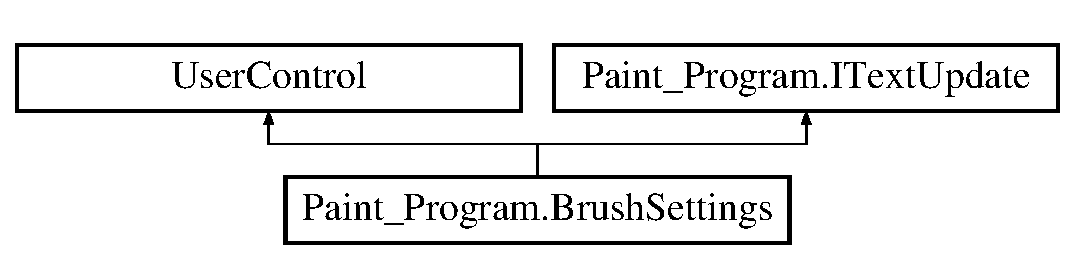
\includegraphics[height=2.000000cm]{class_paint___program_1_1_brush_settings}
\end{center}
\end{figure}
\subsection*{Public Member Functions}
\begin{DoxyCompactItemize}
\item 
\mbox{\hyperlink{class_paint___program_1_1_brush_settings_a70080ac2deafd89e2181a30fff984c2d}{Brush\+Settings}} ()
\item 
void \mbox{\hyperlink{class_paint___program_1_1_brush_settings_aca47f3fee40766ced37ffc395b63cde0}{Check\+Change}} ()
\item 
void \mbox{\hyperlink{class_paint___program_1_1_brush_settings_a0669e5f09b62b9545e408f39689f30ed}{Update\+Text}} ()
\end{DoxyCompactItemize}
\subsection*{Protected Member Functions}
\begin{DoxyCompactItemize}
\item 
override void \mbox{\hyperlink{class_paint___program_1_1_brush_settings_a8b0b64c70a489eb664e73de7b3fe9f9c}{Dispose}} (bool disposing)
\begin{DoxyCompactList}\small\item\em Clean up any resources being used. \end{DoxyCompactList}\end{DoxyCompactItemize}
\subsection*{Private Member Functions}
\begin{DoxyCompactItemize}
\item 
void \mbox{\hyperlink{class_paint___program_1_1_brush_settings_a6b5c3a5900da47314538884ab4105b68}{p\+Prime\+\_\+\+Paint}} (object sender, Paint\+Event\+Args e)
\item 
void \mbox{\hyperlink{class_paint___program_1_1_brush_settings_afe09accaa86f4448f40ddba23ba97abe}{p\+Prime\+\_\+\+Click}} (object sender, Event\+Args e)
\item 
void \mbox{\hyperlink{class_paint___program_1_1_brush_settings_a3d006a8ba7eda56d0d50ce035216c34d}{p\+Sec\+\_\+\+Click}} (object sender, Event\+Args e)
\item 
void \mbox{\hyperlink{class_paint___program_1_1_brush_settings_aa21e17cb46e250b5fb82b1e675dfe768}{tb\+Size\+\_\+\+Value\+Changed}} (object sender, Event\+Args e)
\item 
void \mbox{\hyperlink{class_paint___program_1_1_brush_settings_ac22200ba660ed7ef86423947efb74005}{tb\+Hardness\+\_\+\+Value\+Changed}} (object sender, Event\+Args e)
\item 
void \mbox{\hyperlink{class_paint___program_1_1_brush_settings_a9d332d1302bbf06495360c3a281bd49b}{Initialize\+Component}} ()
\begin{DoxyCompactList}\small\item\em Required method for Designer support -\/ do not modify the contents of this method with the code editor. \end{DoxyCompactList}\end{DoxyCompactItemize}
\subsection*{Private Attributes}
\begin{DoxyCompactItemize}
\item 
Background\+Worker \mbox{\hyperlink{class_paint___program_1_1_brush_settings_a4a6c7587cfe067c706a8a4bf6dad9687}{bw}}
\item 
System.\+Component\+Model.\+I\+Container \mbox{\hyperlink{class_paint___program_1_1_brush_settings_ac77b6db502083ba592247e0eb007b752}{components}} = null
\begin{DoxyCompactList}\small\item\em Required designer variable. \end{DoxyCompactList}\item 
System.\+Windows.\+Forms.\+Label \mbox{\hyperlink{class_paint___program_1_1_brush_settings_ad1374b70dcfd1117d237d46167098107}{l\+Prime}}
\item 
System.\+Windows.\+Forms.\+Label \mbox{\hyperlink{class_paint___program_1_1_brush_settings_a60325fa004c05787a228d967d573f4d8}{l\+Sec}}
\item 
System.\+Windows.\+Forms.\+Panel \mbox{\hyperlink{class_paint___program_1_1_brush_settings_aa26b8d7e9bd76be17ad0af0dfae26b88}{p\+Prime}}
\item 
System.\+Windows.\+Forms.\+Panel \mbox{\hyperlink{class_paint___program_1_1_brush_settings_ae307f3b6b6590fccaa8312c6640ef307}{p\+Sec}}
\item 
System.\+Windows.\+Forms.\+Track\+Bar \mbox{\hyperlink{class_paint___program_1_1_brush_settings_aab6f4a0f6015a47c64a140d940730766}{tb\+Size}}
\item 
System.\+Windows.\+Forms.\+Label \mbox{\hyperlink{class_paint___program_1_1_brush_settings_a9a046fcd4dcc4a3947164cd28b1db6cd}{l\+Size}}
\item 
System.\+Windows.\+Forms.\+Label \mbox{\hyperlink{class_paint___program_1_1_brush_settings_a6188606b564d51909bb795f534259f5c}{l\+Hard}}
\item 
System.\+Windows.\+Forms.\+Track\+Bar \mbox{\hyperlink{class_paint___program_1_1_brush_settings_a77762235bb3accadb1cbd086a37847c0}{tb\+Hardness}}
\item 
System.\+Windows.\+Forms.\+Color\+Dialog \mbox{\hyperlink{class_paint___program_1_1_brush_settings_acfe4bdbac1c6a99a434ff8d8fe91aadb}{cd\+Picker}}
\item 
System.\+Windows.\+Forms.\+Picture\+Box \mbox{\hyperlink{class_paint___program_1_1_brush_settings_a21f90465fb5e4e5ae932019b57142815}{picture\+Box1}}
\end{DoxyCompactItemize}


\subsection{Constructor \& Destructor Documentation}
\mbox{\Hypertarget{class_paint___program_1_1_brush_settings_a70080ac2deafd89e2181a30fff984c2d}\label{class_paint___program_1_1_brush_settings_a70080ac2deafd89e2181a30fff984c2d}} 
\index{Paint\+\_\+\+Program\+::\+Brush\+Settings@{Paint\+\_\+\+Program\+::\+Brush\+Settings}!Brush\+Settings@{Brush\+Settings}}
\index{Brush\+Settings@{Brush\+Settings}!Paint\+\_\+\+Program\+::\+Brush\+Settings@{Paint\+\_\+\+Program\+::\+Brush\+Settings}}
\subsubsection{\texorpdfstring{Brush\+Settings()}{BrushSettings()}}
{\footnotesize\ttfamily Paint\+\_\+\+Program.\+Brush\+Settings.\+Brush\+Settings (\begin{DoxyParamCaption}{ }\end{DoxyParamCaption})\hspace{0.3cm}{\ttfamily [inline]}}



\subsection{Member Function Documentation}
\mbox{\Hypertarget{class_paint___program_1_1_brush_settings_aca47f3fee40766ced37ffc395b63cde0}\label{class_paint___program_1_1_brush_settings_aca47f3fee40766ced37ffc395b63cde0}} 
\index{Paint\+\_\+\+Program\+::\+Brush\+Settings@{Paint\+\_\+\+Program\+::\+Brush\+Settings}!Check\+Change@{Check\+Change}}
\index{Check\+Change@{Check\+Change}!Paint\+\_\+\+Program\+::\+Brush\+Settings@{Paint\+\_\+\+Program\+::\+Brush\+Settings}}
\subsubsection{\texorpdfstring{Check\+Change()}{CheckChange()}}
{\footnotesize\ttfamily void Paint\+\_\+\+Program.\+Brush\+Settings.\+Check\+Change (\begin{DoxyParamCaption}{ }\end{DoxyParamCaption})\hspace{0.3cm}{\ttfamily [inline]}}

\mbox{\Hypertarget{class_paint___program_1_1_brush_settings_a8b0b64c70a489eb664e73de7b3fe9f9c}\label{class_paint___program_1_1_brush_settings_a8b0b64c70a489eb664e73de7b3fe9f9c}} 
\index{Paint\+\_\+\+Program\+::\+Brush\+Settings@{Paint\+\_\+\+Program\+::\+Brush\+Settings}!Dispose@{Dispose}}
\index{Dispose@{Dispose}!Paint\+\_\+\+Program\+::\+Brush\+Settings@{Paint\+\_\+\+Program\+::\+Brush\+Settings}}
\subsubsection{\texorpdfstring{Dispose()}{Dispose()}}
{\footnotesize\ttfamily override void Paint\+\_\+\+Program.\+Brush\+Settings.\+Dispose (\begin{DoxyParamCaption}\item[{bool}]{disposing }\end{DoxyParamCaption})\hspace{0.3cm}{\ttfamily [inline]}, {\ttfamily [protected]}}



Clean up any resources being used. 


\begin{DoxyParams}{Parameters}
{\em disposing} & true if managed resources should be disposed; otherwise, false.\\
\hline
\end{DoxyParams}
\mbox{\Hypertarget{class_paint___program_1_1_brush_settings_a9d332d1302bbf06495360c3a281bd49b}\label{class_paint___program_1_1_brush_settings_a9d332d1302bbf06495360c3a281bd49b}} 
\index{Paint\+\_\+\+Program\+::\+Brush\+Settings@{Paint\+\_\+\+Program\+::\+Brush\+Settings}!Initialize\+Component@{Initialize\+Component}}
\index{Initialize\+Component@{Initialize\+Component}!Paint\+\_\+\+Program\+::\+Brush\+Settings@{Paint\+\_\+\+Program\+::\+Brush\+Settings}}
\subsubsection{\texorpdfstring{Initialize\+Component()}{InitializeComponent()}}
{\footnotesize\ttfamily void Paint\+\_\+\+Program.\+Brush\+Settings.\+Initialize\+Component (\begin{DoxyParamCaption}{ }\end{DoxyParamCaption})\hspace{0.3cm}{\ttfamily [inline]}, {\ttfamily [private]}}



Required method for Designer support -\/ do not modify the contents of this method with the code editor. 

\mbox{\Hypertarget{class_paint___program_1_1_brush_settings_afe09accaa86f4448f40ddba23ba97abe}\label{class_paint___program_1_1_brush_settings_afe09accaa86f4448f40ddba23ba97abe}} 
\index{Paint\+\_\+\+Program\+::\+Brush\+Settings@{Paint\+\_\+\+Program\+::\+Brush\+Settings}!p\+Prime\+\_\+\+Click@{p\+Prime\+\_\+\+Click}}
\index{p\+Prime\+\_\+\+Click@{p\+Prime\+\_\+\+Click}!Paint\+\_\+\+Program\+::\+Brush\+Settings@{Paint\+\_\+\+Program\+::\+Brush\+Settings}}
\subsubsection{\texorpdfstring{p\+Prime\+\_\+\+Click()}{pPrime\_Click()}}
{\footnotesize\ttfamily void Paint\+\_\+\+Program.\+Brush\+Settings.\+p\+Prime\+\_\+\+Click (\begin{DoxyParamCaption}\item[{object}]{sender,  }\item[{Event\+Args}]{e }\end{DoxyParamCaption})\hspace{0.3cm}{\ttfamily [inline]}, {\ttfamily [private]}}

\mbox{\Hypertarget{class_paint___program_1_1_brush_settings_a6b5c3a5900da47314538884ab4105b68}\label{class_paint___program_1_1_brush_settings_a6b5c3a5900da47314538884ab4105b68}} 
\index{Paint\+\_\+\+Program\+::\+Brush\+Settings@{Paint\+\_\+\+Program\+::\+Brush\+Settings}!p\+Prime\+\_\+\+Paint@{p\+Prime\+\_\+\+Paint}}
\index{p\+Prime\+\_\+\+Paint@{p\+Prime\+\_\+\+Paint}!Paint\+\_\+\+Program\+::\+Brush\+Settings@{Paint\+\_\+\+Program\+::\+Brush\+Settings}}
\subsubsection{\texorpdfstring{p\+Prime\+\_\+\+Paint()}{pPrime\_Paint()}}
{\footnotesize\ttfamily void Paint\+\_\+\+Program.\+Brush\+Settings.\+p\+Prime\+\_\+\+Paint (\begin{DoxyParamCaption}\item[{object}]{sender,  }\item[{Paint\+Event\+Args}]{e }\end{DoxyParamCaption})\hspace{0.3cm}{\ttfamily [inline]}, {\ttfamily [private]}}

\mbox{\Hypertarget{class_paint___program_1_1_brush_settings_a3d006a8ba7eda56d0d50ce035216c34d}\label{class_paint___program_1_1_brush_settings_a3d006a8ba7eda56d0d50ce035216c34d}} 
\index{Paint\+\_\+\+Program\+::\+Brush\+Settings@{Paint\+\_\+\+Program\+::\+Brush\+Settings}!p\+Sec\+\_\+\+Click@{p\+Sec\+\_\+\+Click}}
\index{p\+Sec\+\_\+\+Click@{p\+Sec\+\_\+\+Click}!Paint\+\_\+\+Program\+::\+Brush\+Settings@{Paint\+\_\+\+Program\+::\+Brush\+Settings}}
\subsubsection{\texorpdfstring{p\+Sec\+\_\+\+Click()}{pSec\_Click()}}
{\footnotesize\ttfamily void Paint\+\_\+\+Program.\+Brush\+Settings.\+p\+Sec\+\_\+\+Click (\begin{DoxyParamCaption}\item[{object}]{sender,  }\item[{Event\+Args}]{e }\end{DoxyParamCaption})\hspace{0.3cm}{\ttfamily [inline]}, {\ttfamily [private]}}

\mbox{\Hypertarget{class_paint___program_1_1_brush_settings_ac22200ba660ed7ef86423947efb74005}\label{class_paint___program_1_1_brush_settings_ac22200ba660ed7ef86423947efb74005}} 
\index{Paint\+\_\+\+Program\+::\+Brush\+Settings@{Paint\+\_\+\+Program\+::\+Brush\+Settings}!tb\+Hardness\+\_\+\+Value\+Changed@{tb\+Hardness\+\_\+\+Value\+Changed}}
\index{tb\+Hardness\+\_\+\+Value\+Changed@{tb\+Hardness\+\_\+\+Value\+Changed}!Paint\+\_\+\+Program\+::\+Brush\+Settings@{Paint\+\_\+\+Program\+::\+Brush\+Settings}}
\subsubsection{\texorpdfstring{tb\+Hardness\+\_\+\+Value\+Changed()}{tbHardness\_ValueChanged()}}
{\footnotesize\ttfamily void Paint\+\_\+\+Program.\+Brush\+Settings.\+tb\+Hardness\+\_\+\+Value\+Changed (\begin{DoxyParamCaption}\item[{object}]{sender,  }\item[{Event\+Args}]{e }\end{DoxyParamCaption})\hspace{0.3cm}{\ttfamily [inline]}, {\ttfamily [private]}}

\mbox{\Hypertarget{class_paint___program_1_1_brush_settings_aa21e17cb46e250b5fb82b1e675dfe768}\label{class_paint___program_1_1_brush_settings_aa21e17cb46e250b5fb82b1e675dfe768}} 
\index{Paint\+\_\+\+Program\+::\+Brush\+Settings@{Paint\+\_\+\+Program\+::\+Brush\+Settings}!tb\+Size\+\_\+\+Value\+Changed@{tb\+Size\+\_\+\+Value\+Changed}}
\index{tb\+Size\+\_\+\+Value\+Changed@{tb\+Size\+\_\+\+Value\+Changed}!Paint\+\_\+\+Program\+::\+Brush\+Settings@{Paint\+\_\+\+Program\+::\+Brush\+Settings}}
\subsubsection{\texorpdfstring{tb\+Size\+\_\+\+Value\+Changed()}{tbSize\_ValueChanged()}}
{\footnotesize\ttfamily void Paint\+\_\+\+Program.\+Brush\+Settings.\+tb\+Size\+\_\+\+Value\+Changed (\begin{DoxyParamCaption}\item[{object}]{sender,  }\item[{Event\+Args}]{e }\end{DoxyParamCaption})\hspace{0.3cm}{\ttfamily [inline]}, {\ttfamily [private]}}

\mbox{\Hypertarget{class_paint___program_1_1_brush_settings_a0669e5f09b62b9545e408f39689f30ed}\label{class_paint___program_1_1_brush_settings_a0669e5f09b62b9545e408f39689f30ed}} 
\index{Paint\+\_\+\+Program\+::\+Brush\+Settings@{Paint\+\_\+\+Program\+::\+Brush\+Settings}!Update\+Text@{Update\+Text}}
\index{Update\+Text@{Update\+Text}!Paint\+\_\+\+Program\+::\+Brush\+Settings@{Paint\+\_\+\+Program\+::\+Brush\+Settings}}
\subsubsection{\texorpdfstring{Update\+Text()}{UpdateText()}}
{\footnotesize\ttfamily void Paint\+\_\+\+Program.\+Brush\+Settings.\+Update\+Text (\begin{DoxyParamCaption}{ }\end{DoxyParamCaption})\hspace{0.3cm}{\ttfamily [inline]}}



Implements \mbox{\hyperlink{interface_paint___program_1_1_i_text_update_ad1e94db137571608917117e9a6f7479b}{Paint\+\_\+\+Program.\+I\+Text\+Update}}.



\subsection{Member Data Documentation}
\mbox{\Hypertarget{class_paint___program_1_1_brush_settings_a4a6c7587cfe067c706a8a4bf6dad9687}\label{class_paint___program_1_1_brush_settings_a4a6c7587cfe067c706a8a4bf6dad9687}} 
\index{Paint\+\_\+\+Program\+::\+Brush\+Settings@{Paint\+\_\+\+Program\+::\+Brush\+Settings}!bw@{bw}}
\index{bw@{bw}!Paint\+\_\+\+Program\+::\+Brush\+Settings@{Paint\+\_\+\+Program\+::\+Brush\+Settings}}
\subsubsection{\texorpdfstring{bw}{bw}}
{\footnotesize\ttfamily Background\+Worker Paint\+\_\+\+Program.\+Brush\+Settings.\+bw\hspace{0.3cm}{\ttfamily [private]}}

\mbox{\Hypertarget{class_paint___program_1_1_brush_settings_acfe4bdbac1c6a99a434ff8d8fe91aadb}\label{class_paint___program_1_1_brush_settings_acfe4bdbac1c6a99a434ff8d8fe91aadb}} 
\index{Paint\+\_\+\+Program\+::\+Brush\+Settings@{Paint\+\_\+\+Program\+::\+Brush\+Settings}!cd\+Picker@{cd\+Picker}}
\index{cd\+Picker@{cd\+Picker}!Paint\+\_\+\+Program\+::\+Brush\+Settings@{Paint\+\_\+\+Program\+::\+Brush\+Settings}}
\subsubsection{\texorpdfstring{cd\+Picker}{cdPicker}}
{\footnotesize\ttfamily System.\+Windows.\+Forms.\+Color\+Dialog Paint\+\_\+\+Program.\+Brush\+Settings.\+cd\+Picker\hspace{0.3cm}{\ttfamily [private]}}

\mbox{\Hypertarget{class_paint___program_1_1_brush_settings_ac77b6db502083ba592247e0eb007b752}\label{class_paint___program_1_1_brush_settings_ac77b6db502083ba592247e0eb007b752}} 
\index{Paint\+\_\+\+Program\+::\+Brush\+Settings@{Paint\+\_\+\+Program\+::\+Brush\+Settings}!components@{components}}
\index{components@{components}!Paint\+\_\+\+Program\+::\+Brush\+Settings@{Paint\+\_\+\+Program\+::\+Brush\+Settings}}
\subsubsection{\texorpdfstring{components}{components}}
{\footnotesize\ttfamily System.\+Component\+Model.\+I\+Container Paint\+\_\+\+Program.\+Brush\+Settings.\+components = null\hspace{0.3cm}{\ttfamily [private]}}



Required designer variable. 

\mbox{\Hypertarget{class_paint___program_1_1_brush_settings_a6188606b564d51909bb795f534259f5c}\label{class_paint___program_1_1_brush_settings_a6188606b564d51909bb795f534259f5c}} 
\index{Paint\+\_\+\+Program\+::\+Brush\+Settings@{Paint\+\_\+\+Program\+::\+Brush\+Settings}!l\+Hard@{l\+Hard}}
\index{l\+Hard@{l\+Hard}!Paint\+\_\+\+Program\+::\+Brush\+Settings@{Paint\+\_\+\+Program\+::\+Brush\+Settings}}
\subsubsection{\texorpdfstring{l\+Hard}{lHard}}
{\footnotesize\ttfamily System.\+Windows.\+Forms.\+Label Paint\+\_\+\+Program.\+Brush\+Settings.\+l\+Hard\hspace{0.3cm}{\ttfamily [private]}}

\mbox{\Hypertarget{class_paint___program_1_1_brush_settings_ad1374b70dcfd1117d237d46167098107}\label{class_paint___program_1_1_brush_settings_ad1374b70dcfd1117d237d46167098107}} 
\index{Paint\+\_\+\+Program\+::\+Brush\+Settings@{Paint\+\_\+\+Program\+::\+Brush\+Settings}!l\+Prime@{l\+Prime}}
\index{l\+Prime@{l\+Prime}!Paint\+\_\+\+Program\+::\+Brush\+Settings@{Paint\+\_\+\+Program\+::\+Brush\+Settings}}
\subsubsection{\texorpdfstring{l\+Prime}{lPrime}}
{\footnotesize\ttfamily System.\+Windows.\+Forms.\+Label Paint\+\_\+\+Program.\+Brush\+Settings.\+l\+Prime\hspace{0.3cm}{\ttfamily [private]}}

\mbox{\Hypertarget{class_paint___program_1_1_brush_settings_a60325fa004c05787a228d967d573f4d8}\label{class_paint___program_1_1_brush_settings_a60325fa004c05787a228d967d573f4d8}} 
\index{Paint\+\_\+\+Program\+::\+Brush\+Settings@{Paint\+\_\+\+Program\+::\+Brush\+Settings}!l\+Sec@{l\+Sec}}
\index{l\+Sec@{l\+Sec}!Paint\+\_\+\+Program\+::\+Brush\+Settings@{Paint\+\_\+\+Program\+::\+Brush\+Settings}}
\subsubsection{\texorpdfstring{l\+Sec}{lSec}}
{\footnotesize\ttfamily System.\+Windows.\+Forms.\+Label Paint\+\_\+\+Program.\+Brush\+Settings.\+l\+Sec\hspace{0.3cm}{\ttfamily [private]}}

\mbox{\Hypertarget{class_paint___program_1_1_brush_settings_a9a046fcd4dcc4a3947164cd28b1db6cd}\label{class_paint___program_1_1_brush_settings_a9a046fcd4dcc4a3947164cd28b1db6cd}} 
\index{Paint\+\_\+\+Program\+::\+Brush\+Settings@{Paint\+\_\+\+Program\+::\+Brush\+Settings}!l\+Size@{l\+Size}}
\index{l\+Size@{l\+Size}!Paint\+\_\+\+Program\+::\+Brush\+Settings@{Paint\+\_\+\+Program\+::\+Brush\+Settings}}
\subsubsection{\texorpdfstring{l\+Size}{lSize}}
{\footnotesize\ttfamily System.\+Windows.\+Forms.\+Label Paint\+\_\+\+Program.\+Brush\+Settings.\+l\+Size\hspace{0.3cm}{\ttfamily [private]}}

\mbox{\Hypertarget{class_paint___program_1_1_brush_settings_a21f90465fb5e4e5ae932019b57142815}\label{class_paint___program_1_1_brush_settings_a21f90465fb5e4e5ae932019b57142815}} 
\index{Paint\+\_\+\+Program\+::\+Brush\+Settings@{Paint\+\_\+\+Program\+::\+Brush\+Settings}!picture\+Box1@{picture\+Box1}}
\index{picture\+Box1@{picture\+Box1}!Paint\+\_\+\+Program\+::\+Brush\+Settings@{Paint\+\_\+\+Program\+::\+Brush\+Settings}}
\subsubsection{\texorpdfstring{picture\+Box1}{pictureBox1}}
{\footnotesize\ttfamily System.\+Windows.\+Forms.\+Picture\+Box Paint\+\_\+\+Program.\+Brush\+Settings.\+picture\+Box1\hspace{0.3cm}{\ttfamily [private]}}

\mbox{\Hypertarget{class_paint___program_1_1_brush_settings_aa26b8d7e9bd76be17ad0af0dfae26b88}\label{class_paint___program_1_1_brush_settings_aa26b8d7e9bd76be17ad0af0dfae26b88}} 
\index{Paint\+\_\+\+Program\+::\+Brush\+Settings@{Paint\+\_\+\+Program\+::\+Brush\+Settings}!p\+Prime@{p\+Prime}}
\index{p\+Prime@{p\+Prime}!Paint\+\_\+\+Program\+::\+Brush\+Settings@{Paint\+\_\+\+Program\+::\+Brush\+Settings}}
\subsubsection{\texorpdfstring{p\+Prime}{pPrime}}
{\footnotesize\ttfamily System.\+Windows.\+Forms.\+Panel Paint\+\_\+\+Program.\+Brush\+Settings.\+p\+Prime\hspace{0.3cm}{\ttfamily [private]}}

\mbox{\Hypertarget{class_paint___program_1_1_brush_settings_ae307f3b6b6590fccaa8312c6640ef307}\label{class_paint___program_1_1_brush_settings_ae307f3b6b6590fccaa8312c6640ef307}} 
\index{Paint\+\_\+\+Program\+::\+Brush\+Settings@{Paint\+\_\+\+Program\+::\+Brush\+Settings}!p\+Sec@{p\+Sec}}
\index{p\+Sec@{p\+Sec}!Paint\+\_\+\+Program\+::\+Brush\+Settings@{Paint\+\_\+\+Program\+::\+Brush\+Settings}}
\subsubsection{\texorpdfstring{p\+Sec}{pSec}}
{\footnotesize\ttfamily System.\+Windows.\+Forms.\+Panel Paint\+\_\+\+Program.\+Brush\+Settings.\+p\+Sec\hspace{0.3cm}{\ttfamily [private]}}

\mbox{\Hypertarget{class_paint___program_1_1_brush_settings_a77762235bb3accadb1cbd086a37847c0}\label{class_paint___program_1_1_brush_settings_a77762235bb3accadb1cbd086a37847c0}} 
\index{Paint\+\_\+\+Program\+::\+Brush\+Settings@{Paint\+\_\+\+Program\+::\+Brush\+Settings}!tb\+Hardness@{tb\+Hardness}}
\index{tb\+Hardness@{tb\+Hardness}!Paint\+\_\+\+Program\+::\+Brush\+Settings@{Paint\+\_\+\+Program\+::\+Brush\+Settings}}
\subsubsection{\texorpdfstring{tb\+Hardness}{tbHardness}}
{\footnotesize\ttfamily System.\+Windows.\+Forms.\+Track\+Bar Paint\+\_\+\+Program.\+Brush\+Settings.\+tb\+Hardness\hspace{0.3cm}{\ttfamily [private]}}

\mbox{\Hypertarget{class_paint___program_1_1_brush_settings_aab6f4a0f6015a47c64a140d940730766}\label{class_paint___program_1_1_brush_settings_aab6f4a0f6015a47c64a140d940730766}} 
\index{Paint\+\_\+\+Program\+::\+Brush\+Settings@{Paint\+\_\+\+Program\+::\+Brush\+Settings}!tb\+Size@{tb\+Size}}
\index{tb\+Size@{tb\+Size}!Paint\+\_\+\+Program\+::\+Brush\+Settings@{Paint\+\_\+\+Program\+::\+Brush\+Settings}}
\subsubsection{\texorpdfstring{tb\+Size}{tbSize}}
{\footnotesize\ttfamily System.\+Windows.\+Forms.\+Track\+Bar Paint\+\_\+\+Program.\+Brush\+Settings.\+tb\+Size\hspace{0.3cm}{\ttfamily [private]}}



The documentation for this class was generated from the following files\+:\begin{DoxyCompactItemize}
\item 
Paint Program/\mbox{\hyperlink{_brush_settings_8cs}{Brush\+Settings.\+cs}}\item 
Paint Program/\mbox{\hyperlink{_brush_settings_8_designer_8cs}{Brush\+Settings.\+Designer.\+cs}}\end{DoxyCompactItemize}

\hypertarget{class_paint___program_1_1_brush_tool}{}\section{Paint\+\_\+\+Program.\+Brush\+Tool Class Reference}
\label{class_paint___program_1_1_brush_tool}\index{Paint\+\_\+\+Program.\+Brush\+Tool@{Paint\+\_\+\+Program.\+Brush\+Tool}}
Inheritance diagram for Paint\+\_\+\+Program.\+Brush\+Tool\+:\begin{figure}[H]
\begin{center}
\leavevmode
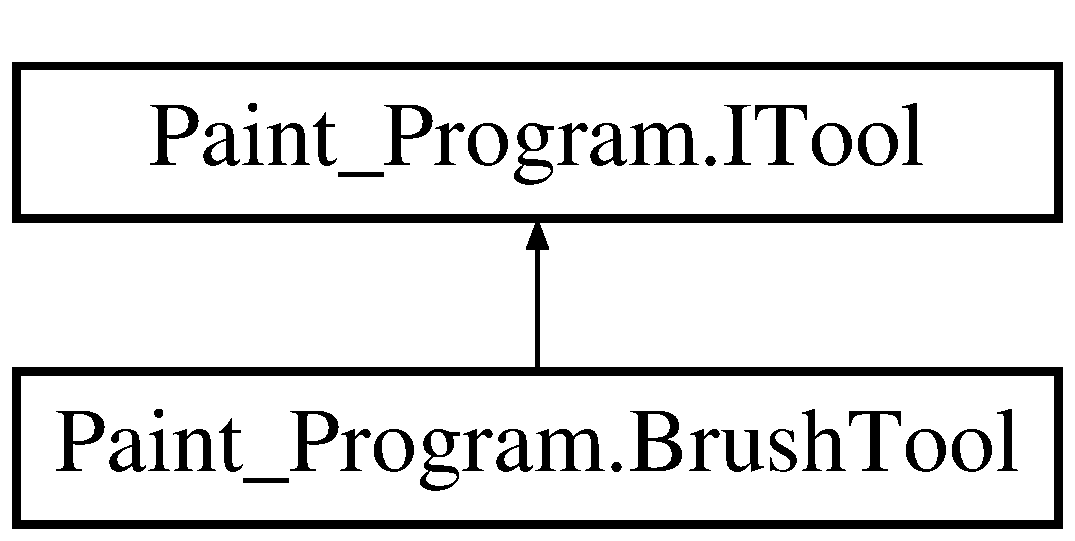
\includegraphics[height=2.000000cm]{class_paint___program_1_1_brush_tool}
\end{center}
\end{figure}
\subsection*{Public Member Functions}
\begin{DoxyCompactItemize}
\item 
\mbox{\hyperlink{class_paint___program_1_1_brush_tool_aab33da2c4f8f8040ec6947ce6f2d4c74}{Brush\+Tool}} ()
\item 
void \mbox{\hyperlink{class_paint___program_1_1_brush_tool_a8cfef3d531b3e9dcb37d81a5ac0a9ad5}{Init}} ()
\item 
string \mbox{\hyperlink{class_paint___program_1_1_brush_tool_a7cc103269b01a6367edce7c994443739}{Get\+Tool\+Icon\+Path}} ()
\item 
void \mbox{\hyperlink{class_paint___program_1_1_brush_tool_a66b7dbcbb7af665e48b14d9e70a8d22d}{On\+Mouse\+Down}} (object sender, Mouse\+Event\+Args e)
\item 
void \mbox{\hyperlink{class_paint___program_1_1_brush_tool_a4246e31217a616bf6bd251ac2b7ac4e3}{On\+Mouse\+Move}} (object sender, Mouse\+Event\+Args e)
\item 
void \mbox{\hyperlink{class_paint___program_1_1_brush_tool_a20c7beba691866bed3cea6a63400d005}{On\+Mouse\+Up}} (object sender, Mouse\+Event\+Args e)
\item 
bool \mbox{\hyperlink{class_paint___program_1_1_brush_tool_a854fff02dd8dfc6016dcb91b4f7d08f9}{is\+Initalized}} ()
\item 
Bitmap \mbox{\hyperlink{class_paint___program_1_1_brush_tool_ae96d4b9560f8d271694abd1e727dd14c}{Get\+Tool\+Layer}} ()
\item 
bool \mbox{\hyperlink{class_paint___program_1_1_brush_tool_ae96d027fe5ef110b5b00802a2d842a15}{Requires\+Layer\+Data}} ()
\item 
void \mbox{\hyperlink{class_paint___program_1_1_brush_tool_a7419f5d4bfddc97bcd3562171d6625cd}{Set\+Layer\+Data}} (Bitmap bit)
\item 
string \mbox{\hyperlink{class_paint___program_1_1_brush_tool_a29d903eb044890b73e06dd9aac2f5b5e}{Get\+Tool\+Tip}} ()
\item 
void \mbox{\hyperlink{class_paint___program_1_1_brush_tool_ab66c41c9ec1f7175fd0a073cf1dacae9}{Update\+Interface\+Layer}} ()
\end{DoxyCompactItemize}
\subsection*{Private Member Functions}
\begin{DoxyCompactItemize}
\item 
void \mbox{\hyperlink{class_paint___program_1_1_brush_tool_ac008b1a1276758fc91ccb3504ddbe2a2}{update\+Brush}} ()
\end{DoxyCompactItemize}
\subsection*{Private Attributes}
\begin{DoxyCompactItemize}
\item 
Graphics \mbox{\hyperlink{class_paint___program_1_1_brush_tool_ada03533308b687fb5aad5a97e39a2418}{graphics}}
\item 
int \mbox{\hyperlink{class_paint___program_1_1_brush_tool_a2d11ac1381688670b77779849c220256}{width}}
\item 
int \mbox{\hyperlink{class_paint___program_1_1_brush_tool_a74fa3f15b3521feddeab58e5da3e794c}{height}}
\item 
bool \mbox{\hyperlink{class_paint___program_1_1_brush_tool_a38e63e44faf4b844b17525f6b64e166b}{b\+Mouse\+Down}}
\item 
bool \mbox{\hyperlink{class_paint___program_1_1_brush_tool_a3bf38746d897988af50ce9d863eaf70b}{b\+Init}}
\item 
Point \mbox{\hyperlink{class_paint___program_1_1_brush_tool_a2686971a90a27e64e904106fa8893841}{p\+Old}}
\item 
Point \mbox{\hyperlink{class_paint___program_1_1_brush_tool_a6d266f7303b546970257227c86dbacf7}{p\+New}}
\item 
Pen \mbox{\hyperlink{class_paint___program_1_1_brush_tool_a5346ef502ccfafa6f49ed704383a7fe5}{pen}}
\item 
Color \mbox{\hyperlink{class_paint___program_1_1_brush_tool_ab15d64ae81405a6edc9c0731975d2b8d}{primary\+Color}}
\item 
Color \mbox{\hyperlink{class_paint___program_1_1_brush_tool_ae5d888beaa07df91858d531a4a0bd5a5}{secondary\+Color}}
\end{DoxyCompactItemize}


\subsection{Constructor \& Destructor Documentation}
\mbox{\Hypertarget{class_paint___program_1_1_brush_tool_aab33da2c4f8f8040ec6947ce6f2d4c74}\label{class_paint___program_1_1_brush_tool_aab33da2c4f8f8040ec6947ce6f2d4c74}} 
\index{Paint\+\_\+\+Program\+::\+Brush\+Tool@{Paint\+\_\+\+Program\+::\+Brush\+Tool}!Brush\+Tool@{Brush\+Tool}}
\index{Brush\+Tool@{Brush\+Tool}!Paint\+\_\+\+Program\+::\+Brush\+Tool@{Paint\+\_\+\+Program\+::\+Brush\+Tool}}
\subsubsection{\texorpdfstring{Brush\+Tool()}{BrushTool()}}
{\footnotesize\ttfamily Paint\+\_\+\+Program.\+Brush\+Tool.\+Brush\+Tool (\begin{DoxyParamCaption}{ }\end{DoxyParamCaption})\hspace{0.3cm}{\ttfamily [inline]}}



\subsection{Member Function Documentation}
\mbox{\Hypertarget{class_paint___program_1_1_brush_tool_a7cc103269b01a6367edce7c994443739}\label{class_paint___program_1_1_brush_tool_a7cc103269b01a6367edce7c994443739}} 
\index{Paint\+\_\+\+Program\+::\+Brush\+Tool@{Paint\+\_\+\+Program\+::\+Brush\+Tool}!Get\+Tool\+Icon\+Path@{Get\+Tool\+Icon\+Path}}
\index{Get\+Tool\+Icon\+Path@{Get\+Tool\+Icon\+Path}!Paint\+\_\+\+Program\+::\+Brush\+Tool@{Paint\+\_\+\+Program\+::\+Brush\+Tool}}
\subsubsection{\texorpdfstring{Get\+Tool\+Icon\+Path()}{GetToolIconPath()}}
{\footnotesize\ttfamily string Paint\+\_\+\+Program.\+Brush\+Tool.\+Get\+Tool\+Icon\+Path (\begin{DoxyParamCaption}{ }\end{DoxyParamCaption})\hspace{0.3cm}{\ttfamily [inline]}}



Implements \mbox{\hyperlink{interface_paint___program_1_1_i_tool_aa057d2f99c59d7bec0215dcad2da1b72}{Paint\+\_\+\+Program.\+I\+Tool}}.

\mbox{\Hypertarget{class_paint___program_1_1_brush_tool_ae96d4b9560f8d271694abd1e727dd14c}\label{class_paint___program_1_1_brush_tool_ae96d4b9560f8d271694abd1e727dd14c}} 
\index{Paint\+\_\+\+Program\+::\+Brush\+Tool@{Paint\+\_\+\+Program\+::\+Brush\+Tool}!Get\+Tool\+Layer@{Get\+Tool\+Layer}}
\index{Get\+Tool\+Layer@{Get\+Tool\+Layer}!Paint\+\_\+\+Program\+::\+Brush\+Tool@{Paint\+\_\+\+Program\+::\+Brush\+Tool}}
\subsubsection{\texorpdfstring{Get\+Tool\+Layer()}{GetToolLayer()}}
{\footnotesize\ttfamily Bitmap Paint\+\_\+\+Program.\+Brush\+Tool.\+Get\+Tool\+Layer (\begin{DoxyParamCaption}{ }\end{DoxyParamCaption})\hspace{0.3cm}{\ttfamily [inline]}}



Implements \mbox{\hyperlink{interface_paint___program_1_1_i_tool_a9b057905515f42a988c166a6a40318e0}{Paint\+\_\+\+Program.\+I\+Tool}}.

\mbox{\Hypertarget{class_paint___program_1_1_brush_tool_a29d903eb044890b73e06dd9aac2f5b5e}\label{class_paint___program_1_1_brush_tool_a29d903eb044890b73e06dd9aac2f5b5e}} 
\index{Paint\+\_\+\+Program\+::\+Brush\+Tool@{Paint\+\_\+\+Program\+::\+Brush\+Tool}!Get\+Tool\+Tip@{Get\+Tool\+Tip}}
\index{Get\+Tool\+Tip@{Get\+Tool\+Tip}!Paint\+\_\+\+Program\+::\+Brush\+Tool@{Paint\+\_\+\+Program\+::\+Brush\+Tool}}
\subsubsection{\texorpdfstring{Get\+Tool\+Tip()}{GetToolTip()}}
{\footnotesize\ttfamily string Paint\+\_\+\+Program.\+Brush\+Tool.\+Get\+Tool\+Tip (\begin{DoxyParamCaption}{ }\end{DoxyParamCaption})\hspace{0.3cm}{\ttfamily [inline]}}



Implements \mbox{\hyperlink{interface_paint___program_1_1_i_tool_ac11f1591587144b6e74f5767bbf1df56}{Paint\+\_\+\+Program.\+I\+Tool}}.

\mbox{\Hypertarget{class_paint___program_1_1_brush_tool_a8cfef3d531b3e9dcb37d81a5ac0a9ad5}\label{class_paint___program_1_1_brush_tool_a8cfef3d531b3e9dcb37d81a5ac0a9ad5}} 
\index{Paint\+\_\+\+Program\+::\+Brush\+Tool@{Paint\+\_\+\+Program\+::\+Brush\+Tool}!Init@{Init}}
\index{Init@{Init}!Paint\+\_\+\+Program\+::\+Brush\+Tool@{Paint\+\_\+\+Program\+::\+Brush\+Tool}}
\subsubsection{\texorpdfstring{Init()}{Init()}}
{\footnotesize\ttfamily void Paint\+\_\+\+Program.\+Brush\+Tool.\+Init (\begin{DoxyParamCaption}{ }\end{DoxyParamCaption})\hspace{0.3cm}{\ttfamily [inline]}}



Implements \mbox{\hyperlink{interface_paint___program_1_1_i_tool_af823123a30fbda34e24e907243241046}{Paint\+\_\+\+Program.\+I\+Tool}}.

\mbox{\Hypertarget{class_paint___program_1_1_brush_tool_a854fff02dd8dfc6016dcb91b4f7d08f9}\label{class_paint___program_1_1_brush_tool_a854fff02dd8dfc6016dcb91b4f7d08f9}} 
\index{Paint\+\_\+\+Program\+::\+Brush\+Tool@{Paint\+\_\+\+Program\+::\+Brush\+Tool}!is\+Initalized@{is\+Initalized}}
\index{is\+Initalized@{is\+Initalized}!Paint\+\_\+\+Program\+::\+Brush\+Tool@{Paint\+\_\+\+Program\+::\+Brush\+Tool}}
\subsubsection{\texorpdfstring{is\+Initalized()}{isInitalized()}}
{\footnotesize\ttfamily bool Paint\+\_\+\+Program.\+Brush\+Tool.\+is\+Initalized (\begin{DoxyParamCaption}{ }\end{DoxyParamCaption})\hspace{0.3cm}{\ttfamily [inline]}}



Implements \mbox{\hyperlink{interface_paint___program_1_1_i_tool_a951b844bcbf47a6c306104fa86be7a5d}{Paint\+\_\+\+Program.\+I\+Tool}}.

\mbox{\Hypertarget{class_paint___program_1_1_brush_tool_a66b7dbcbb7af665e48b14d9e70a8d22d}\label{class_paint___program_1_1_brush_tool_a66b7dbcbb7af665e48b14d9e70a8d22d}} 
\index{Paint\+\_\+\+Program\+::\+Brush\+Tool@{Paint\+\_\+\+Program\+::\+Brush\+Tool}!On\+Mouse\+Down@{On\+Mouse\+Down}}
\index{On\+Mouse\+Down@{On\+Mouse\+Down}!Paint\+\_\+\+Program\+::\+Brush\+Tool@{Paint\+\_\+\+Program\+::\+Brush\+Tool}}
\subsubsection{\texorpdfstring{On\+Mouse\+Down()}{OnMouseDown()}}
{\footnotesize\ttfamily void Paint\+\_\+\+Program.\+Brush\+Tool.\+On\+Mouse\+Down (\begin{DoxyParamCaption}\item[{object}]{sender,  }\item[{Mouse\+Event\+Args}]{e }\end{DoxyParamCaption})\hspace{0.3cm}{\ttfamily [inline]}}



Implements \mbox{\hyperlink{interface_paint___program_1_1_i_tool_a73d8797f4f2b1e0d8efe8aadcd44e840}{Paint\+\_\+\+Program.\+I\+Tool}}.

\mbox{\Hypertarget{class_paint___program_1_1_brush_tool_a4246e31217a616bf6bd251ac2b7ac4e3}\label{class_paint___program_1_1_brush_tool_a4246e31217a616bf6bd251ac2b7ac4e3}} 
\index{Paint\+\_\+\+Program\+::\+Brush\+Tool@{Paint\+\_\+\+Program\+::\+Brush\+Tool}!On\+Mouse\+Move@{On\+Mouse\+Move}}
\index{On\+Mouse\+Move@{On\+Mouse\+Move}!Paint\+\_\+\+Program\+::\+Brush\+Tool@{Paint\+\_\+\+Program\+::\+Brush\+Tool}}
\subsubsection{\texorpdfstring{On\+Mouse\+Move()}{OnMouseMove()}}
{\footnotesize\ttfamily void Paint\+\_\+\+Program.\+Brush\+Tool.\+On\+Mouse\+Move (\begin{DoxyParamCaption}\item[{object}]{sender,  }\item[{Mouse\+Event\+Args}]{e }\end{DoxyParamCaption})\hspace{0.3cm}{\ttfamily [inline]}}



Implements \mbox{\hyperlink{interface_paint___program_1_1_i_tool_a6a1cbe840b5cfc8a9b9463cc21590845}{Paint\+\_\+\+Program.\+I\+Tool}}.

\mbox{\Hypertarget{class_paint___program_1_1_brush_tool_a20c7beba691866bed3cea6a63400d005}\label{class_paint___program_1_1_brush_tool_a20c7beba691866bed3cea6a63400d005}} 
\index{Paint\+\_\+\+Program\+::\+Brush\+Tool@{Paint\+\_\+\+Program\+::\+Brush\+Tool}!On\+Mouse\+Up@{On\+Mouse\+Up}}
\index{On\+Mouse\+Up@{On\+Mouse\+Up}!Paint\+\_\+\+Program\+::\+Brush\+Tool@{Paint\+\_\+\+Program\+::\+Brush\+Tool}}
\subsubsection{\texorpdfstring{On\+Mouse\+Up()}{OnMouseUp()}}
{\footnotesize\ttfamily void Paint\+\_\+\+Program.\+Brush\+Tool.\+On\+Mouse\+Up (\begin{DoxyParamCaption}\item[{object}]{sender,  }\item[{Mouse\+Event\+Args}]{e }\end{DoxyParamCaption})\hspace{0.3cm}{\ttfamily [inline]}}



Implements \mbox{\hyperlink{interface_paint___program_1_1_i_tool_a47984c2879213022f1684c07f7bba73e}{Paint\+\_\+\+Program.\+I\+Tool}}.

\mbox{\Hypertarget{class_paint___program_1_1_brush_tool_ae96d027fe5ef110b5b00802a2d842a15}\label{class_paint___program_1_1_brush_tool_ae96d027fe5ef110b5b00802a2d842a15}} 
\index{Paint\+\_\+\+Program\+::\+Brush\+Tool@{Paint\+\_\+\+Program\+::\+Brush\+Tool}!Requires\+Layer\+Data@{Requires\+Layer\+Data}}
\index{Requires\+Layer\+Data@{Requires\+Layer\+Data}!Paint\+\_\+\+Program\+::\+Brush\+Tool@{Paint\+\_\+\+Program\+::\+Brush\+Tool}}
\subsubsection{\texorpdfstring{Requires\+Layer\+Data()}{RequiresLayerData()}}
{\footnotesize\ttfamily bool Paint\+\_\+\+Program.\+Brush\+Tool.\+Requires\+Layer\+Data (\begin{DoxyParamCaption}{ }\end{DoxyParamCaption})\hspace{0.3cm}{\ttfamily [inline]}}



Implements \mbox{\hyperlink{interface_paint___program_1_1_i_tool_a6d45b6c48da8130ae41db3a66cdaef9a}{Paint\+\_\+\+Program.\+I\+Tool}}.

\mbox{\Hypertarget{class_paint___program_1_1_brush_tool_a7419f5d4bfddc97bcd3562171d6625cd}\label{class_paint___program_1_1_brush_tool_a7419f5d4bfddc97bcd3562171d6625cd}} 
\index{Paint\+\_\+\+Program\+::\+Brush\+Tool@{Paint\+\_\+\+Program\+::\+Brush\+Tool}!Set\+Layer\+Data@{Set\+Layer\+Data}}
\index{Set\+Layer\+Data@{Set\+Layer\+Data}!Paint\+\_\+\+Program\+::\+Brush\+Tool@{Paint\+\_\+\+Program\+::\+Brush\+Tool}}
\subsubsection{\texorpdfstring{Set\+Layer\+Data()}{SetLayerData()}}
{\footnotesize\ttfamily void Paint\+\_\+\+Program.\+Brush\+Tool.\+Set\+Layer\+Data (\begin{DoxyParamCaption}\item[{Bitmap}]{bit }\end{DoxyParamCaption})\hspace{0.3cm}{\ttfamily [inline]}}



Implements \mbox{\hyperlink{interface_paint___program_1_1_i_tool_a2d3e63715dfe04075d27dacf367d1633}{Paint\+\_\+\+Program.\+I\+Tool}}.

\mbox{\Hypertarget{class_paint___program_1_1_brush_tool_ac008b1a1276758fc91ccb3504ddbe2a2}\label{class_paint___program_1_1_brush_tool_ac008b1a1276758fc91ccb3504ddbe2a2}} 
\index{Paint\+\_\+\+Program\+::\+Brush\+Tool@{Paint\+\_\+\+Program\+::\+Brush\+Tool}!update\+Brush@{update\+Brush}}
\index{update\+Brush@{update\+Brush}!Paint\+\_\+\+Program\+::\+Brush\+Tool@{Paint\+\_\+\+Program\+::\+Brush\+Tool}}
\subsubsection{\texorpdfstring{update\+Brush()}{updateBrush()}}
{\footnotesize\ttfamily void Paint\+\_\+\+Program.\+Brush\+Tool.\+update\+Brush (\begin{DoxyParamCaption}{ }\end{DoxyParamCaption})\hspace{0.3cm}{\ttfamily [inline]}, {\ttfamily [private]}}

\mbox{\Hypertarget{class_paint___program_1_1_brush_tool_ab66c41c9ec1f7175fd0a073cf1dacae9}\label{class_paint___program_1_1_brush_tool_ab66c41c9ec1f7175fd0a073cf1dacae9}} 
\index{Paint\+\_\+\+Program\+::\+Brush\+Tool@{Paint\+\_\+\+Program\+::\+Brush\+Tool}!Update\+Interface\+Layer@{Update\+Interface\+Layer}}
\index{Update\+Interface\+Layer@{Update\+Interface\+Layer}!Paint\+\_\+\+Program\+::\+Brush\+Tool@{Paint\+\_\+\+Program\+::\+Brush\+Tool}}
\subsubsection{\texorpdfstring{Update\+Interface\+Layer()}{UpdateInterfaceLayer()}}
{\footnotesize\ttfamily void Paint\+\_\+\+Program.\+Brush\+Tool.\+Update\+Interface\+Layer (\begin{DoxyParamCaption}{ }\end{DoxyParamCaption})\hspace{0.3cm}{\ttfamily [inline]}}



Implements \mbox{\hyperlink{interface_paint___program_1_1_i_tool_a36db75d29e88dfd739f658633c40e955}{Paint\+\_\+\+Program.\+I\+Tool}}.



\subsection{Member Data Documentation}
\mbox{\Hypertarget{class_paint___program_1_1_brush_tool_a3bf38746d897988af50ce9d863eaf70b}\label{class_paint___program_1_1_brush_tool_a3bf38746d897988af50ce9d863eaf70b}} 
\index{Paint\+\_\+\+Program\+::\+Brush\+Tool@{Paint\+\_\+\+Program\+::\+Brush\+Tool}!b\+Init@{b\+Init}}
\index{b\+Init@{b\+Init}!Paint\+\_\+\+Program\+::\+Brush\+Tool@{Paint\+\_\+\+Program\+::\+Brush\+Tool}}
\subsubsection{\texorpdfstring{b\+Init}{bInit}}
{\footnotesize\ttfamily bool Paint\+\_\+\+Program.\+Brush\+Tool.\+b\+Init\hspace{0.3cm}{\ttfamily [private]}}

\mbox{\Hypertarget{class_paint___program_1_1_brush_tool_a38e63e44faf4b844b17525f6b64e166b}\label{class_paint___program_1_1_brush_tool_a38e63e44faf4b844b17525f6b64e166b}} 
\index{Paint\+\_\+\+Program\+::\+Brush\+Tool@{Paint\+\_\+\+Program\+::\+Brush\+Tool}!b\+Mouse\+Down@{b\+Mouse\+Down}}
\index{b\+Mouse\+Down@{b\+Mouse\+Down}!Paint\+\_\+\+Program\+::\+Brush\+Tool@{Paint\+\_\+\+Program\+::\+Brush\+Tool}}
\subsubsection{\texorpdfstring{b\+Mouse\+Down}{bMouseDown}}
{\footnotesize\ttfamily bool Paint\+\_\+\+Program.\+Brush\+Tool.\+b\+Mouse\+Down\hspace{0.3cm}{\ttfamily [private]}}

\mbox{\Hypertarget{class_paint___program_1_1_brush_tool_ada03533308b687fb5aad5a97e39a2418}\label{class_paint___program_1_1_brush_tool_ada03533308b687fb5aad5a97e39a2418}} 
\index{Paint\+\_\+\+Program\+::\+Brush\+Tool@{Paint\+\_\+\+Program\+::\+Brush\+Tool}!graphics@{graphics}}
\index{graphics@{graphics}!Paint\+\_\+\+Program\+::\+Brush\+Tool@{Paint\+\_\+\+Program\+::\+Brush\+Tool}}
\subsubsection{\texorpdfstring{graphics}{graphics}}
{\footnotesize\ttfamily Graphics Paint\+\_\+\+Program.\+Brush\+Tool.\+graphics\hspace{0.3cm}{\ttfamily [private]}}

\mbox{\Hypertarget{class_paint___program_1_1_brush_tool_a74fa3f15b3521feddeab58e5da3e794c}\label{class_paint___program_1_1_brush_tool_a74fa3f15b3521feddeab58e5da3e794c}} 
\index{Paint\+\_\+\+Program\+::\+Brush\+Tool@{Paint\+\_\+\+Program\+::\+Brush\+Tool}!height@{height}}
\index{height@{height}!Paint\+\_\+\+Program\+::\+Brush\+Tool@{Paint\+\_\+\+Program\+::\+Brush\+Tool}}
\subsubsection{\texorpdfstring{height}{height}}
{\footnotesize\ttfamily int Paint\+\_\+\+Program.\+Brush\+Tool.\+height\hspace{0.3cm}{\ttfamily [private]}}

\mbox{\Hypertarget{class_paint___program_1_1_brush_tool_a5346ef502ccfafa6f49ed704383a7fe5}\label{class_paint___program_1_1_brush_tool_a5346ef502ccfafa6f49ed704383a7fe5}} 
\index{Paint\+\_\+\+Program\+::\+Brush\+Tool@{Paint\+\_\+\+Program\+::\+Brush\+Tool}!pen@{pen}}
\index{pen@{pen}!Paint\+\_\+\+Program\+::\+Brush\+Tool@{Paint\+\_\+\+Program\+::\+Brush\+Tool}}
\subsubsection{\texorpdfstring{pen}{pen}}
{\footnotesize\ttfamily Pen Paint\+\_\+\+Program.\+Brush\+Tool.\+pen\hspace{0.3cm}{\ttfamily [private]}}

\mbox{\Hypertarget{class_paint___program_1_1_brush_tool_a6d266f7303b546970257227c86dbacf7}\label{class_paint___program_1_1_brush_tool_a6d266f7303b546970257227c86dbacf7}} 
\index{Paint\+\_\+\+Program\+::\+Brush\+Tool@{Paint\+\_\+\+Program\+::\+Brush\+Tool}!p\+New@{p\+New}}
\index{p\+New@{p\+New}!Paint\+\_\+\+Program\+::\+Brush\+Tool@{Paint\+\_\+\+Program\+::\+Brush\+Tool}}
\subsubsection{\texorpdfstring{p\+New}{pNew}}
{\footnotesize\ttfamily Point Paint\+\_\+\+Program.\+Brush\+Tool.\+p\+New\hspace{0.3cm}{\ttfamily [private]}}

\mbox{\Hypertarget{class_paint___program_1_1_brush_tool_a2686971a90a27e64e904106fa8893841}\label{class_paint___program_1_1_brush_tool_a2686971a90a27e64e904106fa8893841}} 
\index{Paint\+\_\+\+Program\+::\+Brush\+Tool@{Paint\+\_\+\+Program\+::\+Brush\+Tool}!p\+Old@{p\+Old}}
\index{p\+Old@{p\+Old}!Paint\+\_\+\+Program\+::\+Brush\+Tool@{Paint\+\_\+\+Program\+::\+Brush\+Tool}}
\subsubsection{\texorpdfstring{p\+Old}{pOld}}
{\footnotesize\ttfamily Point Paint\+\_\+\+Program.\+Brush\+Tool.\+p\+Old\hspace{0.3cm}{\ttfamily [private]}}

\mbox{\Hypertarget{class_paint___program_1_1_brush_tool_ab15d64ae81405a6edc9c0731975d2b8d}\label{class_paint___program_1_1_brush_tool_ab15d64ae81405a6edc9c0731975d2b8d}} 
\index{Paint\+\_\+\+Program\+::\+Brush\+Tool@{Paint\+\_\+\+Program\+::\+Brush\+Tool}!primary\+Color@{primary\+Color}}
\index{primary\+Color@{primary\+Color}!Paint\+\_\+\+Program\+::\+Brush\+Tool@{Paint\+\_\+\+Program\+::\+Brush\+Tool}}
\subsubsection{\texorpdfstring{primary\+Color}{primaryColor}}
{\footnotesize\ttfamily Color Paint\+\_\+\+Program.\+Brush\+Tool.\+primary\+Color\hspace{0.3cm}{\ttfamily [private]}}

\mbox{\Hypertarget{class_paint___program_1_1_brush_tool_ae5d888beaa07df91858d531a4a0bd5a5}\label{class_paint___program_1_1_brush_tool_ae5d888beaa07df91858d531a4a0bd5a5}} 
\index{Paint\+\_\+\+Program\+::\+Brush\+Tool@{Paint\+\_\+\+Program\+::\+Brush\+Tool}!secondary\+Color@{secondary\+Color}}
\index{secondary\+Color@{secondary\+Color}!Paint\+\_\+\+Program\+::\+Brush\+Tool@{Paint\+\_\+\+Program\+::\+Brush\+Tool}}
\subsubsection{\texorpdfstring{secondary\+Color}{secondaryColor}}
{\footnotesize\ttfamily Color Paint\+\_\+\+Program.\+Brush\+Tool.\+secondary\+Color\hspace{0.3cm}{\ttfamily [private]}}

\mbox{\Hypertarget{class_paint___program_1_1_brush_tool_a2d11ac1381688670b77779849c220256}\label{class_paint___program_1_1_brush_tool_a2d11ac1381688670b77779849c220256}} 
\index{Paint\+\_\+\+Program\+::\+Brush\+Tool@{Paint\+\_\+\+Program\+::\+Brush\+Tool}!width@{width}}
\index{width@{width}!Paint\+\_\+\+Program\+::\+Brush\+Tool@{Paint\+\_\+\+Program\+::\+Brush\+Tool}}
\subsubsection{\texorpdfstring{width}{width}}
{\footnotesize\ttfamily int Paint\+\_\+\+Program.\+Brush\+Tool.\+width\hspace{0.3cm}{\ttfamily [private]}}



The documentation for this class was generated from the following file\+:\begin{DoxyCompactItemize}
\item 
Paint Program/\mbox{\hyperlink{_brush_tool_8cs}{Brush\+Tool.\+cs}}\end{DoxyCompactItemize}

\hypertarget{class_paint___program_1_1_canvas}{}\section{Paint\+\_\+\+Program.\+Canvas Class Reference}
\label{class_paint___program_1_1_canvas}\index{Paint\+\_\+\+Program.\+Canvas@{Paint\+\_\+\+Program.\+Canvas}}


Class handling the main rendering of the layers, and interfacing with tools  


Inheritance diagram for Paint\+\_\+\+Program.\+Canvas\+:\begin{figure}[H]
\begin{center}
\leavevmode
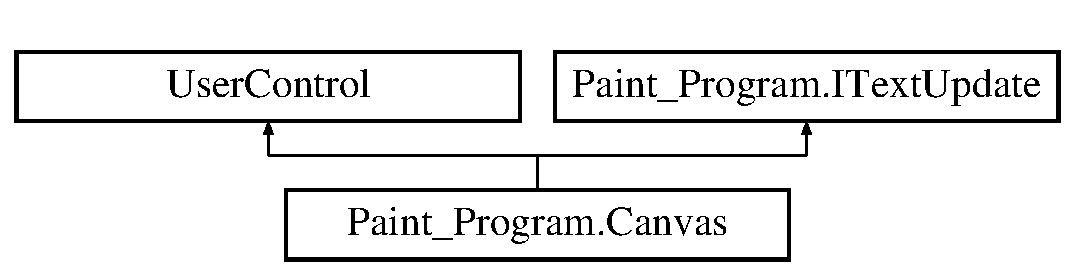
\includegraphics[height=2.000000cm]{class_paint___program_1_1_canvas}
\end{center}
\end{figure}
\subsection*{Public Member Functions}
\begin{DoxyCompactItemize}
\item 
\mbox{\hyperlink{class_paint___program_1_1_canvas_add693d71442d497fe310ccab15a4b22f}{Canvas}} (int pw, int ph)
\item 
\mbox{\hyperlink{class_paint___program_1_1_canvas_af40bf569df831849e1c369dec074cc41}{Canvas}} (int w, int h, int pw, int ph)
\item 
void \mbox{\hyperlink{class_paint___program_1_1_canvas_ab2cd1e144d21d48fcd8e123df1b7214c}{Init\+Canvas}} ()
\begin{DoxyCompactList}\small\item\em Initializes all main components that the canvas interfaces with \end{DoxyCompactList}\item 
void \mbox{\hyperlink{class_paint___program_1_1_canvas_a2c266c354fa86bc892a2eebf183d04f3}{Zoom\+In}} ()
\begin{DoxyCompactList}\small\item\em Zooms canvas in by 10\% \end{DoxyCompactList}\item 
void \mbox{\hyperlink{class_paint___program_1_1_canvas_a6470498d99b7f3fb2d2b26116c2abb44}{Zoom\+Out}} ()
\begin{DoxyCompactList}\small\item\em Zooms canvas out by 10\% \end{DoxyCompactList}\item 
void \mbox{\hyperlink{class_paint___program_1_1_canvas_a472cbf23dbea24d0bd70e2267529307a}{Update\+Positions}} (object sender)
\begin{DoxyCompactList}\small\item\em Updates the positions of the different components in the application \end{DoxyCompactList}\item 
void \mbox{\hyperlink{class_paint___program_1_1_canvas_a08e5d5aa35c75a7e6c64db752a79df8e}{Handle\+Mouse\+Down}} (object sender, Mouse\+Event\+Args e)
\begin{DoxyCompactList}\small\item\em Handles mouse down events and sends event data to tools \end{DoxyCompactList}\item 
void \mbox{\hyperlink{class_paint___program_1_1_canvas_a9e3612510a869438dad1e5bd0ec3870e}{Handle\+Mouse\+Up}} (object sender, Mouse\+Event\+Args e)
\begin{DoxyCompactList}\small\item\em Handles mouse up events and sends event data to tools \end{DoxyCompactList}\item 
void \mbox{\hyperlink{class_paint___program_1_1_canvas_a469df114198596cb65df4a22fcabc685}{Handle\+Mouse\+Move}} (object sender, Mouse\+Event\+Args e)
\begin{DoxyCompactList}\small\item\em Handles mouse move events and sends event data to tools \end{DoxyCompactList}\item 
void \mbox{\hyperlink{class_paint___program_1_1_canvas_addf9e6c4759c930a9aaba20125f66a24}{Update\+Canvas}} (Graphics graphics)
\begin{DoxyCompactList}\small\item\em Called periodically to render the image to the screen \end{DoxyCompactList}\item 
void \mbox{\hyperlink{class_paint___program_1_1_canvas_a3ba07590551cf4f24d942302e90db30f}{Set\+Pause}} (bool b)
\begin{DoxyCompactList}\small\item\em Sets the pause flag to start or stop rendering of the main canvas \end{DoxyCompactList}\item 
Bitmap \mbox{\hyperlink{class_paint___program_1_1_canvas_a1dad48a553831296e7920219e8614a6f}{Get\+Bitmap}} ()
\begin{DoxyCompactList}\small\item\em Renders all layers to a new Bitmap \end{DoxyCompactList}\item 
void \mbox{\hyperlink{class_paint___program_1_1_canvas_a8548f36df2fefafcbcc23d857592ddc6}{Show\+Tools}} ()
\begin{DoxyCompactList}\small\item\em Displays the tool strip \end{DoxyCompactList}\item 
void \mbox{\hyperlink{class_paint___program_1_1_canvas_a26985c4da349cdddbe1c91bfef8e1a10}{Hide\+Tools}} ()
\begin{DoxyCompactList}\small\item\em Hides the tool strip \end{DoxyCompactList}\item 
void \mbox{\hyperlink{class_paint___program_1_1_canvas_ad80b3ef48814a229e01a330b49344f3b}{Update\+Text}} ()
\begin{DoxyCompactList}\small\item\em Calls the Update Text method for all classes that implement \mbox{\hyperlink{interface_paint___program_1_1_i_text_update}{I\+Text\+Update}} \end{DoxyCompactList}\item 
void \mbox{\hyperlink{class_paint___program_1_1_canvas_ac7d12ff2474d5bca00d8d399f0f6f17f}{Trash}} ()
\begin{DoxyCompactList}\small\item\em Disposes all resources \end{DoxyCompactList}\end{DoxyCompactItemize}
\subsection*{Static Public Member Functions}
\begin{DoxyCompactItemize}
\item 
static void \mbox{\hyperlink{class_paint___program_1_1_canvas_a94533b18db7d150d723ecaaf789d406b}{Handle\+Watermark}} (Graphics graphics)
\begin{DoxyCompactList}\small\item\em Handles rendering the watermark to a Bitmap using the provided Graphics object \end{DoxyCompactList}\end{DoxyCompactItemize}
\subsection*{Public Attributes}
\begin{DoxyCompactItemize}
\item 
List$<$ Tool\+Strip\+Button $>$ \mbox{\hyperlink{class_paint___program_1_1_canvas_ada97231f783b6eb308b9e54523729bd5}{Tool\+Buttons}}
\end{DoxyCompactItemize}
\subsection*{Protected Member Functions}
\begin{DoxyCompactItemize}
\item 
override void \mbox{\hyperlink{class_paint___program_1_1_canvas_aafaa253cb056ff1725f6c1c7c74895a7}{Dispose}} (bool disposing)
\begin{DoxyCompactList}\small\item\em Clean up any resources being used. \end{DoxyCompactList}\end{DoxyCompactItemize}
\subsection*{Private Member Functions}
\begin{DoxyCompactItemize}
\item 
void \mbox{\hyperlink{class_paint___program_1_1_canvas_a7fa8707eec6c1868ec18f7151146bfae}{Init\+Tools}} ()
\begin{DoxyCompactList}\small\item\em Adds all tools to the tool bar \end{DoxyCompactList}\item 
void \mbox{\hyperlink{class_paint___program_1_1_canvas_a9cf2287e46eb0e4408c936f9d063662e}{Handle\+Tablet\+Data}} (object sender, \mbox{\hyperlink{class_wintab_d_n_1_1_message_received_event_args}{Message\+Received\+Event\+Args}} e)
\begin{DoxyCompactList}\small\item\em \mbox{\hyperlink{namespace_wintab_d_n}{Wintab\+DN}} event handler to interface with U\+SB drawing tablets \end{DoxyCompactList}\item 
void \mbox{\hyperlink{class_paint___program_1_1_canvas_a2b9769c074033d3e7b9782f058adac34}{Handle\+Tool\+Strip\+Item\+Click}} (object sender, Event\+Args e)
\begin{DoxyCompactList}\small\item\em Handles tool changes \end{DoxyCompactList}\item 
void \mbox{\hyperlink{class_paint___program_1_1_canvas_a03a3c5c5aa5410c596ca804543048cd2}{Handle\+Parent\+Resize}} (object sender, Event\+Args e)
\begin{DoxyCompactList}\small\item\em Handles window resize by adjusting the position of all components \end{DoxyCompactList}\item 
Mouse\+Event\+Args \mbox{\hyperlink{class_paint___program_1_1_canvas_ad115e2e049fe0710853b8eb6c87ba578}{Scale\+Mouse\+Event}} (Mouse\+Event\+Args e)
\begin{DoxyCompactList}\small\item\em Scales the mouse event so that when the canvas is zoomed in the mouse is still in the correct location \end{DoxyCompactList}\item 
void \mbox{\hyperlink{class_paint___program_1_1_canvas_a7dcd37fbb4f649a9a52109244cdc06c8}{E\+Display\+Paint}} (object sender, Paint\+Event\+Args e)
\begin{DoxyCompactList}\small\item\em Calls Update\+Graphics() \end{DoxyCompactList}\item 
void \mbox{\hyperlink{class_paint___program_1_1_canvas_a34dfcf5fd2dd88431a7172cce26887ba}{Initialize\+Component}} ()
\begin{DoxyCompactList}\small\item\em Required method for Designer support -\/ do not modify the contents of this method with the code editor. \end{DoxyCompactList}\end{DoxyCompactItemize}
\subsection*{Private Attributes}
\begin{DoxyCompactItemize}
\item 
\mbox{\hyperlink{class_paint___program_1_1_display}{Display}} \mbox{\hyperlink{class_paint___program_1_1_canvas_a062e8c62840a26ff882cc4d04df225ee}{p}}
\item 
Panel \mbox{\hyperlink{class_paint___program_1_1_canvas_a2b8da1cfbec0bf30e3c75ec1b2254e2b}{p\+Scaled}}
\item 
Graphics \mbox{\hyperlink{class_paint___program_1_1_canvas_aa6c67366d90077fa9b0628d9366bcbca}{g}}
\item 
Bitmap \mbox{\hyperlink{class_paint___program_1_1_canvas_a0cc3e58e865cf5a755d4d9f35f70238a}{bg}}
\item 
Bitmap \mbox{\hyperlink{class_paint___program_1_1_canvas_a19a0714ac47bc1320dcc9cefd12b380b}{Grid}}
\item 
const int \mbox{\hyperlink{class_paint___program_1_1_canvas_ac3c70713c3f72a4d4e8663dc90c10285}{G\+Cper\+Frames}} = 100
\item 
int \mbox{\hyperlink{class_paint___program_1_1_canvas_aa8fa583bc964d8ea68628c9b8e7e648a}{canvas\+Width}}
\item 
int \mbox{\hyperlink{class_paint___program_1_1_canvas_abee27e7eab8e6f5afb30044e97de2de2}{canvas\+Height}}
\item 
int \mbox{\hyperlink{class_paint___program_1_1_canvas_a0f7c080162d099242cfa35dc480c3ba9}{max\+Width}}
\item 
int \mbox{\hyperlink{class_paint___program_1_1_canvas_a1a8c4189ce38200f313962cad08a7fe3}{max\+Height}}
\item 
int \mbox{\hyperlink{class_paint___program_1_1_canvas_aaa74adb42b806ce50aa45a9b7501e042}{scroll\+Width}}
\item 
int \mbox{\hyperlink{class_paint___program_1_1_canvas_acc89dc931642d1b1874c96781f67932e}{scroll\+Height}}
\item 
int \mbox{\hyperlink{class_paint___program_1_1_canvas_ab971915f406e70cbe0b793ff8bfa44ad}{ts\+Width}}
\item 
int \mbox{\hyperlink{class_paint___program_1_1_canvas_af7619a49de47ab8a829b7d54cd13fa34}{menu\+Height}}
\item 
int \mbox{\hyperlink{class_paint___program_1_1_canvas_a069f9fb1fdfda2efb72002def8de69b8}{i\+Active\+Tool}}
\item 
bool \mbox{\hyperlink{class_paint___program_1_1_canvas_ae594f00ab27c7c5535b99ef3ea83330f}{is\+Pasued}} = false
\item 
\mbox{\hyperlink{class_paint___program_1_1_layer_view}{Layer\+View}} \mbox{\hyperlink{class_paint___program_1_1_canvas_a76ad801807be5089e7fa17fb5e49cd87}{lv}}
\item 
Tool\+Strip \mbox{\hyperlink{class_paint___program_1_1_canvas_a25f473e57732815bbfd29ece6c8d9e1a}{ts}}
\item 
\mbox{\hyperlink{class_paint___program_1_1_brush_settings}{Brush\+Settings}} \mbox{\hyperlink{class_paint___program_1_1_canvas_a8d4ab120fa6b6a09a21550b9c529ee32}{bs}}
\item 
\mbox{\hyperlink{class_paint___program_1_1_zoom_control}{Zoom\+Control}} \mbox{\hyperlink{class_paint___program_1_1_canvas_ae476a361419679063d08d82be0d75586}{zc}}
\item 
\mbox{\hyperlink{class_paint___program_1_1_tablet_info}{Tablet\+Info}} \mbox{\hyperlink{class_paint___program_1_1_canvas_a82ed26ab78c420733a97cbf4b70cd0c1}{ti}}
\item 
List$<$ \mbox{\hyperlink{interface_paint___program_1_1_i_tool}{I\+Tool}} $>$ \mbox{\hyperlink{class_paint___program_1_1_canvas_aa4c39db74d3d28be21479042ebbb5ac1}{Tools}}
\item 
bool \mbox{\hyperlink{class_paint___program_1_1_canvas_a6b215f6b92ac2e3215da878200ce02b6}{Tools\+Shown}} = true
\item 
System.\+Component\+Model.\+I\+Container \mbox{\hyperlink{class_paint___program_1_1_canvas_a669e31bb19fca7ec4eaa939d5068eed4}{components}} = null
\begin{DoxyCompactList}\small\item\em Required designer variable. \end{DoxyCompactList}\end{DoxyCompactItemize}


\subsection{Detailed Description}
Class handling the main rendering of the layers, and interfacing with tools 



\subsection{Constructor \& Destructor Documentation}
\mbox{\Hypertarget{class_paint___program_1_1_canvas_add693d71442d497fe310ccab15a4b22f}\label{class_paint___program_1_1_canvas_add693d71442d497fe310ccab15a4b22f}} 
\index{Paint\+\_\+\+Program\+::\+Canvas@{Paint\+\_\+\+Program\+::\+Canvas}!Canvas@{Canvas}}
\index{Canvas@{Canvas}!Paint\+\_\+\+Program\+::\+Canvas@{Paint\+\_\+\+Program\+::\+Canvas}}
\subsubsection{\texorpdfstring{Canvas()}{Canvas()}\hspace{0.1cm}{\footnotesize\ttfamily [1/2]}}
{\footnotesize\ttfamily Paint\+\_\+\+Program.\+Canvas.\+Canvas (\begin{DoxyParamCaption}\item[{int}]{pw,  }\item[{int}]{ph }\end{DoxyParamCaption})\hspace{0.3cm}{\ttfamily [inline]}}

\mbox{\Hypertarget{class_paint___program_1_1_canvas_af40bf569df831849e1c369dec074cc41}\label{class_paint___program_1_1_canvas_af40bf569df831849e1c369dec074cc41}} 
\index{Paint\+\_\+\+Program\+::\+Canvas@{Paint\+\_\+\+Program\+::\+Canvas}!Canvas@{Canvas}}
\index{Canvas@{Canvas}!Paint\+\_\+\+Program\+::\+Canvas@{Paint\+\_\+\+Program\+::\+Canvas}}
\subsubsection{\texorpdfstring{Canvas()}{Canvas()}\hspace{0.1cm}{\footnotesize\ttfamily [2/2]}}
{\footnotesize\ttfamily Paint\+\_\+\+Program.\+Canvas.\+Canvas (\begin{DoxyParamCaption}\item[{int}]{w,  }\item[{int}]{h,  }\item[{int}]{pw,  }\item[{int}]{ph }\end{DoxyParamCaption})\hspace{0.3cm}{\ttfamily [inline]}}



\subsection{Member Function Documentation}
\mbox{\Hypertarget{class_paint___program_1_1_canvas_aafaa253cb056ff1725f6c1c7c74895a7}\label{class_paint___program_1_1_canvas_aafaa253cb056ff1725f6c1c7c74895a7}} 
\index{Paint\+\_\+\+Program\+::\+Canvas@{Paint\+\_\+\+Program\+::\+Canvas}!Dispose@{Dispose}}
\index{Dispose@{Dispose}!Paint\+\_\+\+Program\+::\+Canvas@{Paint\+\_\+\+Program\+::\+Canvas}}
\subsubsection{\texorpdfstring{Dispose()}{Dispose()}}
{\footnotesize\ttfamily override void Paint\+\_\+\+Program.\+Canvas.\+Dispose (\begin{DoxyParamCaption}\item[{bool}]{disposing }\end{DoxyParamCaption})\hspace{0.3cm}{\ttfamily [inline]}, {\ttfamily [protected]}}



Clean up any resources being used. 


\begin{DoxyParams}{Parameters}
{\em disposing} & true if managed resources should be disposed; otherwise, false.\\
\hline
\end{DoxyParams}
\mbox{\Hypertarget{class_paint___program_1_1_canvas_a7dcd37fbb4f649a9a52109244cdc06c8}\label{class_paint___program_1_1_canvas_a7dcd37fbb4f649a9a52109244cdc06c8}} 
\index{Paint\+\_\+\+Program\+::\+Canvas@{Paint\+\_\+\+Program\+::\+Canvas}!E\+Display\+Paint@{E\+Display\+Paint}}
\index{E\+Display\+Paint@{E\+Display\+Paint}!Paint\+\_\+\+Program\+::\+Canvas@{Paint\+\_\+\+Program\+::\+Canvas}}
\subsubsection{\texorpdfstring{E\+Display\+Paint()}{EDisplayPaint()}}
{\footnotesize\ttfamily void Paint\+\_\+\+Program.\+Canvas.\+E\+Display\+Paint (\begin{DoxyParamCaption}\item[{object}]{sender,  }\item[{Paint\+Event\+Args}]{e }\end{DoxyParamCaption})\hspace{0.3cm}{\ttfamily [inline]}, {\ttfamily [private]}}



Calls Update\+Graphics() 


\begin{DoxyParams}{Parameters}
{\em sender} & Not Used\\
\hline
{\em e} & Paint\+Event\+Args object where the Graphics property is passed to Update\+Graphics()\\
\hline
\end{DoxyParams}
\mbox{\Hypertarget{class_paint___program_1_1_canvas_a1dad48a553831296e7920219e8614a6f}\label{class_paint___program_1_1_canvas_a1dad48a553831296e7920219e8614a6f}} 
\index{Paint\+\_\+\+Program\+::\+Canvas@{Paint\+\_\+\+Program\+::\+Canvas}!Get\+Bitmap@{Get\+Bitmap}}
\index{Get\+Bitmap@{Get\+Bitmap}!Paint\+\_\+\+Program\+::\+Canvas@{Paint\+\_\+\+Program\+::\+Canvas}}
\subsubsection{\texorpdfstring{Get\+Bitmap()}{GetBitmap()}}
{\footnotesize\ttfamily Bitmap Paint\+\_\+\+Program.\+Canvas.\+Get\+Bitmap (\begin{DoxyParamCaption}{ }\end{DoxyParamCaption})\hspace{0.3cm}{\ttfamily [inline]}}



Renders all layers to a new Bitmap 

\begin{DoxyReturn}{Returns}
Bitmap containing a render of all the layer data
\end{DoxyReturn}
\mbox{\Hypertarget{class_paint___program_1_1_canvas_a08e5d5aa35c75a7e6c64db752a79df8e}\label{class_paint___program_1_1_canvas_a08e5d5aa35c75a7e6c64db752a79df8e}} 
\index{Paint\+\_\+\+Program\+::\+Canvas@{Paint\+\_\+\+Program\+::\+Canvas}!Handle\+Mouse\+Down@{Handle\+Mouse\+Down}}
\index{Handle\+Mouse\+Down@{Handle\+Mouse\+Down}!Paint\+\_\+\+Program\+::\+Canvas@{Paint\+\_\+\+Program\+::\+Canvas}}
\subsubsection{\texorpdfstring{Handle\+Mouse\+Down()}{HandleMouseDown()}}
{\footnotesize\ttfamily void Paint\+\_\+\+Program.\+Canvas.\+Handle\+Mouse\+Down (\begin{DoxyParamCaption}\item[{object}]{sender,  }\item[{Mouse\+Event\+Args}]{e }\end{DoxyParamCaption})\hspace{0.3cm}{\ttfamily [inline]}}



Handles mouse down events and sends event data to tools 


\begin{DoxyParams}{Parameters}
{\em sender} & N/A\\
\hline
{\em e} & Mouse\+Event\+Args containing data of the mouse event\\
\hline
\end{DoxyParams}
\mbox{\Hypertarget{class_paint___program_1_1_canvas_a469df114198596cb65df4a22fcabc685}\label{class_paint___program_1_1_canvas_a469df114198596cb65df4a22fcabc685}} 
\index{Paint\+\_\+\+Program\+::\+Canvas@{Paint\+\_\+\+Program\+::\+Canvas}!Handle\+Mouse\+Move@{Handle\+Mouse\+Move}}
\index{Handle\+Mouse\+Move@{Handle\+Mouse\+Move}!Paint\+\_\+\+Program\+::\+Canvas@{Paint\+\_\+\+Program\+::\+Canvas}}
\subsubsection{\texorpdfstring{Handle\+Mouse\+Move()}{HandleMouseMove()}}
{\footnotesize\ttfamily void Paint\+\_\+\+Program.\+Canvas.\+Handle\+Mouse\+Move (\begin{DoxyParamCaption}\item[{object}]{sender,  }\item[{Mouse\+Event\+Args}]{e }\end{DoxyParamCaption})\hspace{0.3cm}{\ttfamily [inline]}}



Handles mouse move events and sends event data to tools 


\begin{DoxyParams}{Parameters}
{\em sender} & N/A\\
\hline
{\em e} & Mouse\+Event\+Args containing data of the mouse event\\
\hline
\end{DoxyParams}
\mbox{\Hypertarget{class_paint___program_1_1_canvas_a9e3612510a869438dad1e5bd0ec3870e}\label{class_paint___program_1_1_canvas_a9e3612510a869438dad1e5bd0ec3870e}} 
\index{Paint\+\_\+\+Program\+::\+Canvas@{Paint\+\_\+\+Program\+::\+Canvas}!Handle\+Mouse\+Up@{Handle\+Mouse\+Up}}
\index{Handle\+Mouse\+Up@{Handle\+Mouse\+Up}!Paint\+\_\+\+Program\+::\+Canvas@{Paint\+\_\+\+Program\+::\+Canvas}}
\subsubsection{\texorpdfstring{Handle\+Mouse\+Up()}{HandleMouseUp()}}
{\footnotesize\ttfamily void Paint\+\_\+\+Program.\+Canvas.\+Handle\+Mouse\+Up (\begin{DoxyParamCaption}\item[{object}]{sender,  }\item[{Mouse\+Event\+Args}]{e }\end{DoxyParamCaption})\hspace{0.3cm}{\ttfamily [inline]}}



Handles mouse up events and sends event data to tools 


\begin{DoxyParams}{Parameters}
{\em sender} & N/A\\
\hline
{\em e} & Mouse\+Event\+Args containing data of the mouse event\\
\hline
\end{DoxyParams}
\mbox{\Hypertarget{class_paint___program_1_1_canvas_a03a3c5c5aa5410c596ca804543048cd2}\label{class_paint___program_1_1_canvas_a03a3c5c5aa5410c596ca804543048cd2}} 
\index{Paint\+\_\+\+Program\+::\+Canvas@{Paint\+\_\+\+Program\+::\+Canvas}!Handle\+Parent\+Resize@{Handle\+Parent\+Resize}}
\index{Handle\+Parent\+Resize@{Handle\+Parent\+Resize}!Paint\+\_\+\+Program\+::\+Canvas@{Paint\+\_\+\+Program\+::\+Canvas}}
\subsubsection{\texorpdfstring{Handle\+Parent\+Resize()}{HandleParentResize()}}
{\footnotesize\ttfamily void Paint\+\_\+\+Program.\+Canvas.\+Handle\+Parent\+Resize (\begin{DoxyParamCaption}\item[{object}]{sender,  }\item[{Event\+Args}]{e }\end{DoxyParamCaption})\hspace{0.3cm}{\ttfamily [inline]}, {\ttfamily [private]}}



Handles window resize by adjusting the position of all components 


\begin{DoxyParams}{Parameters}
{\em sender} & The parent control of this \mbox{\hyperlink{class_paint___program_1_1_canvas}{Canvas}} class\\
\hline
{\em e} & N/A\\
\hline
\end{DoxyParams}
\mbox{\Hypertarget{class_paint___program_1_1_canvas_a9cf2287e46eb0e4408c936f9d063662e}\label{class_paint___program_1_1_canvas_a9cf2287e46eb0e4408c936f9d063662e}} 
\index{Paint\+\_\+\+Program\+::\+Canvas@{Paint\+\_\+\+Program\+::\+Canvas}!Handle\+Tablet\+Data@{Handle\+Tablet\+Data}}
\index{Handle\+Tablet\+Data@{Handle\+Tablet\+Data}!Paint\+\_\+\+Program\+::\+Canvas@{Paint\+\_\+\+Program\+::\+Canvas}}
\subsubsection{\texorpdfstring{Handle\+Tablet\+Data()}{HandleTabletData()}}
{\footnotesize\ttfamily void Paint\+\_\+\+Program.\+Canvas.\+Handle\+Tablet\+Data (\begin{DoxyParamCaption}\item[{object}]{sender,  }\item[{\mbox{\hyperlink{class_wintab_d_n_1_1_message_received_event_args}{Message\+Received\+Event\+Args}}}]{e }\end{DoxyParamCaption})\hspace{0.3cm}{\ttfamily [inline]}, {\ttfamily [private]}}



\mbox{\hyperlink{namespace_wintab_d_n}{Wintab\+DN}} event handler to interface with U\+SB drawing tablets 


\begin{DoxyParams}{Parameters}
{\em sender} & N/A\\
\hline
{\em e} & Tablet event data\\
\hline
\end{DoxyParams}
\mbox{\Hypertarget{class_paint___program_1_1_canvas_a2b9769c074033d3e7b9782f058adac34}\label{class_paint___program_1_1_canvas_a2b9769c074033d3e7b9782f058adac34}} 
\index{Paint\+\_\+\+Program\+::\+Canvas@{Paint\+\_\+\+Program\+::\+Canvas}!Handle\+Tool\+Strip\+Item\+Click@{Handle\+Tool\+Strip\+Item\+Click}}
\index{Handle\+Tool\+Strip\+Item\+Click@{Handle\+Tool\+Strip\+Item\+Click}!Paint\+\_\+\+Program\+::\+Canvas@{Paint\+\_\+\+Program\+::\+Canvas}}
\subsubsection{\texorpdfstring{Handle\+Tool\+Strip\+Item\+Click()}{HandleToolStripItemClick()}}
{\footnotesize\ttfamily void Paint\+\_\+\+Program.\+Canvas.\+Handle\+Tool\+Strip\+Item\+Click (\begin{DoxyParamCaption}\item[{object}]{sender,  }\item[{Event\+Args}]{e }\end{DoxyParamCaption})\hspace{0.3cm}{\ttfamily [inline]}, {\ttfamily [private]}}



Handles tool changes 


\begin{DoxyParams}{Parameters}
{\em sender} & \\
\hline
{\em e} & \\
\hline
\end{DoxyParams}
\mbox{\Hypertarget{class_paint___program_1_1_canvas_a94533b18db7d150d723ecaaf789d406b}\label{class_paint___program_1_1_canvas_a94533b18db7d150d723ecaaf789d406b}} 
\index{Paint\+\_\+\+Program\+::\+Canvas@{Paint\+\_\+\+Program\+::\+Canvas}!Handle\+Watermark@{Handle\+Watermark}}
\index{Handle\+Watermark@{Handle\+Watermark}!Paint\+\_\+\+Program\+::\+Canvas@{Paint\+\_\+\+Program\+::\+Canvas}}
\subsubsection{\texorpdfstring{Handle\+Watermark()}{HandleWatermark()}}
{\footnotesize\ttfamily static void Paint\+\_\+\+Program.\+Canvas.\+Handle\+Watermark (\begin{DoxyParamCaption}\item[{Graphics}]{graphics }\end{DoxyParamCaption})\hspace{0.3cm}{\ttfamily [inline]}, {\ttfamily [static]}}



Handles rendering the watermark to a Bitmap using the provided Graphics object 


\begin{DoxyParams}{Parameters}
{\em graphics} & Graphics object used to render the watermark\\
\hline
\end{DoxyParams}
\mbox{\Hypertarget{class_paint___program_1_1_canvas_a26985c4da349cdddbe1c91bfef8e1a10}\label{class_paint___program_1_1_canvas_a26985c4da349cdddbe1c91bfef8e1a10}} 
\index{Paint\+\_\+\+Program\+::\+Canvas@{Paint\+\_\+\+Program\+::\+Canvas}!Hide\+Tools@{Hide\+Tools}}
\index{Hide\+Tools@{Hide\+Tools}!Paint\+\_\+\+Program\+::\+Canvas@{Paint\+\_\+\+Program\+::\+Canvas}}
\subsubsection{\texorpdfstring{Hide\+Tools()}{HideTools()}}
{\footnotesize\ttfamily void Paint\+\_\+\+Program.\+Canvas.\+Hide\+Tools (\begin{DoxyParamCaption}{ }\end{DoxyParamCaption})\hspace{0.3cm}{\ttfamily [inline]}}



Hides the tool strip 

\mbox{\Hypertarget{class_paint___program_1_1_canvas_ab2cd1e144d21d48fcd8e123df1b7214c}\label{class_paint___program_1_1_canvas_ab2cd1e144d21d48fcd8e123df1b7214c}} 
\index{Paint\+\_\+\+Program\+::\+Canvas@{Paint\+\_\+\+Program\+::\+Canvas}!Init\+Canvas@{Init\+Canvas}}
\index{Init\+Canvas@{Init\+Canvas}!Paint\+\_\+\+Program\+::\+Canvas@{Paint\+\_\+\+Program\+::\+Canvas}}
\subsubsection{\texorpdfstring{Init\+Canvas()}{InitCanvas()}}
{\footnotesize\ttfamily void Paint\+\_\+\+Program.\+Canvas.\+Init\+Canvas (\begin{DoxyParamCaption}{ }\end{DoxyParamCaption})\hspace{0.3cm}{\ttfamily [inline]}}



Initializes all main components that the canvas interfaces with 

\mbox{\Hypertarget{class_paint___program_1_1_canvas_a34dfcf5fd2dd88431a7172cce26887ba}\label{class_paint___program_1_1_canvas_a34dfcf5fd2dd88431a7172cce26887ba}} 
\index{Paint\+\_\+\+Program\+::\+Canvas@{Paint\+\_\+\+Program\+::\+Canvas}!Initialize\+Component@{Initialize\+Component}}
\index{Initialize\+Component@{Initialize\+Component}!Paint\+\_\+\+Program\+::\+Canvas@{Paint\+\_\+\+Program\+::\+Canvas}}
\subsubsection{\texorpdfstring{Initialize\+Component()}{InitializeComponent()}}
{\footnotesize\ttfamily void Paint\+\_\+\+Program.\+Canvas.\+Initialize\+Component (\begin{DoxyParamCaption}{ }\end{DoxyParamCaption})\hspace{0.3cm}{\ttfamily [inline]}, {\ttfamily [private]}}



Required method for Designer support -\/ do not modify the contents of this method with the code editor. 

\mbox{\Hypertarget{class_paint___program_1_1_canvas_a7fa8707eec6c1868ec18f7151146bfae}\label{class_paint___program_1_1_canvas_a7fa8707eec6c1868ec18f7151146bfae}} 
\index{Paint\+\_\+\+Program\+::\+Canvas@{Paint\+\_\+\+Program\+::\+Canvas}!Init\+Tools@{Init\+Tools}}
\index{Init\+Tools@{Init\+Tools}!Paint\+\_\+\+Program\+::\+Canvas@{Paint\+\_\+\+Program\+::\+Canvas}}
\subsubsection{\texorpdfstring{Init\+Tools()}{InitTools()}}
{\footnotesize\ttfamily void Paint\+\_\+\+Program.\+Canvas.\+Init\+Tools (\begin{DoxyParamCaption}{ }\end{DoxyParamCaption})\hspace{0.3cm}{\ttfamily [inline]}, {\ttfamily [private]}}



Adds all tools to the tool bar 

\mbox{\Hypertarget{class_paint___program_1_1_canvas_ad115e2e049fe0710853b8eb6c87ba578}\label{class_paint___program_1_1_canvas_ad115e2e049fe0710853b8eb6c87ba578}} 
\index{Paint\+\_\+\+Program\+::\+Canvas@{Paint\+\_\+\+Program\+::\+Canvas}!Scale\+Mouse\+Event@{Scale\+Mouse\+Event}}
\index{Scale\+Mouse\+Event@{Scale\+Mouse\+Event}!Paint\+\_\+\+Program\+::\+Canvas@{Paint\+\_\+\+Program\+::\+Canvas}}
\subsubsection{\texorpdfstring{Scale\+Mouse\+Event()}{ScaleMouseEvent()}}
{\footnotesize\ttfamily Mouse\+Event\+Args Paint\+\_\+\+Program.\+Canvas.\+Scale\+Mouse\+Event (\begin{DoxyParamCaption}\item[{Mouse\+Event\+Args}]{e }\end{DoxyParamCaption})\hspace{0.3cm}{\ttfamily [inline]}, {\ttfamily [private]}}



Scales the mouse event so that when the canvas is zoomed in the mouse is still in the correct location 


\begin{DoxyParams}{Parameters}
{\em e} & Mouse\+Event\+Args containing the mouse event data\\
\hline
\end{DoxyParams}
\begin{DoxyReturn}{Returns}

\end{DoxyReturn}
\mbox{\Hypertarget{class_paint___program_1_1_canvas_a3ba07590551cf4f24d942302e90db30f}\label{class_paint___program_1_1_canvas_a3ba07590551cf4f24d942302e90db30f}} 
\index{Paint\+\_\+\+Program\+::\+Canvas@{Paint\+\_\+\+Program\+::\+Canvas}!Set\+Pause@{Set\+Pause}}
\index{Set\+Pause@{Set\+Pause}!Paint\+\_\+\+Program\+::\+Canvas@{Paint\+\_\+\+Program\+::\+Canvas}}
\subsubsection{\texorpdfstring{Set\+Pause()}{SetPause()}}
{\footnotesize\ttfamily void Paint\+\_\+\+Program.\+Canvas.\+Set\+Pause (\begin{DoxyParamCaption}\item[{bool}]{b }\end{DoxyParamCaption})\hspace{0.3cm}{\ttfamily [inline]}}



Sets the pause flag to start or stop rendering of the main canvas 


\begin{DoxyParams}{Parameters}
{\em b} & Boolean value, true stops canvas rendering, false continues rendering \\
\hline
\end{DoxyParams}
\mbox{\Hypertarget{class_paint___program_1_1_canvas_a8548f36df2fefafcbcc23d857592ddc6}\label{class_paint___program_1_1_canvas_a8548f36df2fefafcbcc23d857592ddc6}} 
\index{Paint\+\_\+\+Program\+::\+Canvas@{Paint\+\_\+\+Program\+::\+Canvas}!Show\+Tools@{Show\+Tools}}
\index{Show\+Tools@{Show\+Tools}!Paint\+\_\+\+Program\+::\+Canvas@{Paint\+\_\+\+Program\+::\+Canvas}}
\subsubsection{\texorpdfstring{Show\+Tools()}{ShowTools()}}
{\footnotesize\ttfamily void Paint\+\_\+\+Program.\+Canvas.\+Show\+Tools (\begin{DoxyParamCaption}{ }\end{DoxyParamCaption})\hspace{0.3cm}{\ttfamily [inline]}}



Displays the tool strip 

\mbox{\Hypertarget{class_paint___program_1_1_canvas_ac7d12ff2474d5bca00d8d399f0f6f17f}\label{class_paint___program_1_1_canvas_ac7d12ff2474d5bca00d8d399f0f6f17f}} 
\index{Paint\+\_\+\+Program\+::\+Canvas@{Paint\+\_\+\+Program\+::\+Canvas}!Trash@{Trash}}
\index{Trash@{Trash}!Paint\+\_\+\+Program\+::\+Canvas@{Paint\+\_\+\+Program\+::\+Canvas}}
\subsubsection{\texorpdfstring{Trash()}{Trash()}}
{\footnotesize\ttfamily void Paint\+\_\+\+Program.\+Canvas.\+Trash (\begin{DoxyParamCaption}{ }\end{DoxyParamCaption})\hspace{0.3cm}{\ttfamily [inline]}}



Disposes all resources 

\mbox{\Hypertarget{class_paint___program_1_1_canvas_addf9e6c4759c930a9aaba20125f66a24}\label{class_paint___program_1_1_canvas_addf9e6c4759c930a9aaba20125f66a24}} 
\index{Paint\+\_\+\+Program\+::\+Canvas@{Paint\+\_\+\+Program\+::\+Canvas}!Update\+Canvas@{Update\+Canvas}}
\index{Update\+Canvas@{Update\+Canvas}!Paint\+\_\+\+Program\+::\+Canvas@{Paint\+\_\+\+Program\+::\+Canvas}}
\subsubsection{\texorpdfstring{Update\+Canvas()}{UpdateCanvas()}}
{\footnotesize\ttfamily void Paint\+\_\+\+Program.\+Canvas.\+Update\+Canvas (\begin{DoxyParamCaption}\item[{Graphics}]{graphics }\end{DoxyParamCaption})\hspace{0.3cm}{\ttfamily [inline]}}



Called periodically to render the image to the screen 


\begin{DoxyParams}{Parameters}
{\em graphics} & Graphics object of the Bitmap being rendered to\\
\hline
\end{DoxyParams}
\mbox{\Hypertarget{class_paint___program_1_1_canvas_a472cbf23dbea24d0bd70e2267529307a}\label{class_paint___program_1_1_canvas_a472cbf23dbea24d0bd70e2267529307a}} 
\index{Paint\+\_\+\+Program\+::\+Canvas@{Paint\+\_\+\+Program\+::\+Canvas}!Update\+Positions@{Update\+Positions}}
\index{Update\+Positions@{Update\+Positions}!Paint\+\_\+\+Program\+::\+Canvas@{Paint\+\_\+\+Program\+::\+Canvas}}
\subsubsection{\texorpdfstring{Update\+Positions()}{UpdatePositions()}}
{\footnotesize\ttfamily void Paint\+\_\+\+Program.\+Canvas.\+Update\+Positions (\begin{DoxyParamCaption}\item[{object}]{sender }\end{DoxyParamCaption})\hspace{0.3cm}{\ttfamily [inline]}}



Updates the positions of the different components in the application 


\begin{DoxyParams}{Parameters}
{\em sender} & N/A\\
\hline
\end{DoxyParams}
\mbox{\Hypertarget{class_paint___program_1_1_canvas_ad80b3ef48814a229e01a330b49344f3b}\label{class_paint___program_1_1_canvas_ad80b3ef48814a229e01a330b49344f3b}} 
\index{Paint\+\_\+\+Program\+::\+Canvas@{Paint\+\_\+\+Program\+::\+Canvas}!Update\+Text@{Update\+Text}}
\index{Update\+Text@{Update\+Text}!Paint\+\_\+\+Program\+::\+Canvas@{Paint\+\_\+\+Program\+::\+Canvas}}
\subsubsection{\texorpdfstring{Update\+Text()}{UpdateText()}}
{\footnotesize\ttfamily void Paint\+\_\+\+Program.\+Canvas.\+Update\+Text (\begin{DoxyParamCaption}{ }\end{DoxyParamCaption})\hspace{0.3cm}{\ttfamily [inline]}}



Calls the Update Text method for all classes that implement \mbox{\hyperlink{interface_paint___program_1_1_i_text_update}{I\+Text\+Update}} 



Implements \mbox{\hyperlink{interface_paint___program_1_1_i_text_update_ad1e94db137571608917117e9a6f7479b}{Paint\+\_\+\+Program.\+I\+Text\+Update}}.

\mbox{\Hypertarget{class_paint___program_1_1_canvas_a2c266c354fa86bc892a2eebf183d04f3}\label{class_paint___program_1_1_canvas_a2c266c354fa86bc892a2eebf183d04f3}} 
\index{Paint\+\_\+\+Program\+::\+Canvas@{Paint\+\_\+\+Program\+::\+Canvas}!Zoom\+In@{Zoom\+In}}
\index{Zoom\+In@{Zoom\+In}!Paint\+\_\+\+Program\+::\+Canvas@{Paint\+\_\+\+Program\+::\+Canvas}}
\subsubsection{\texorpdfstring{Zoom\+In()}{ZoomIn()}}
{\footnotesize\ttfamily void Paint\+\_\+\+Program.\+Canvas.\+Zoom\+In (\begin{DoxyParamCaption}{ }\end{DoxyParamCaption})\hspace{0.3cm}{\ttfamily [inline]}}



Zooms canvas in by 10\% 

\mbox{\Hypertarget{class_paint___program_1_1_canvas_a6470498d99b7f3fb2d2b26116c2abb44}\label{class_paint___program_1_1_canvas_a6470498d99b7f3fb2d2b26116c2abb44}} 
\index{Paint\+\_\+\+Program\+::\+Canvas@{Paint\+\_\+\+Program\+::\+Canvas}!Zoom\+Out@{Zoom\+Out}}
\index{Zoom\+Out@{Zoom\+Out}!Paint\+\_\+\+Program\+::\+Canvas@{Paint\+\_\+\+Program\+::\+Canvas}}
\subsubsection{\texorpdfstring{Zoom\+Out()}{ZoomOut()}}
{\footnotesize\ttfamily void Paint\+\_\+\+Program.\+Canvas.\+Zoom\+Out (\begin{DoxyParamCaption}{ }\end{DoxyParamCaption})\hspace{0.3cm}{\ttfamily [inline]}}



Zooms canvas out by 10\% 



\subsection{Member Data Documentation}
\mbox{\Hypertarget{class_paint___program_1_1_canvas_a0cc3e58e865cf5a755d4d9f35f70238a}\label{class_paint___program_1_1_canvas_a0cc3e58e865cf5a755d4d9f35f70238a}} 
\index{Paint\+\_\+\+Program\+::\+Canvas@{Paint\+\_\+\+Program\+::\+Canvas}!bg@{bg}}
\index{bg@{bg}!Paint\+\_\+\+Program\+::\+Canvas@{Paint\+\_\+\+Program\+::\+Canvas}}
\subsubsection{\texorpdfstring{bg}{bg}}
{\footnotesize\ttfamily Bitmap Paint\+\_\+\+Program.\+Canvas.\+bg\hspace{0.3cm}{\ttfamily [private]}}

\mbox{\Hypertarget{class_paint___program_1_1_canvas_a8d4ab120fa6b6a09a21550b9c529ee32}\label{class_paint___program_1_1_canvas_a8d4ab120fa6b6a09a21550b9c529ee32}} 
\index{Paint\+\_\+\+Program\+::\+Canvas@{Paint\+\_\+\+Program\+::\+Canvas}!bs@{bs}}
\index{bs@{bs}!Paint\+\_\+\+Program\+::\+Canvas@{Paint\+\_\+\+Program\+::\+Canvas}}
\subsubsection{\texorpdfstring{bs}{bs}}
{\footnotesize\ttfamily \mbox{\hyperlink{class_paint___program_1_1_brush_settings}{Brush\+Settings}} Paint\+\_\+\+Program.\+Canvas.\+bs\hspace{0.3cm}{\ttfamily [private]}}

\mbox{\Hypertarget{class_paint___program_1_1_canvas_abee27e7eab8e6f5afb30044e97de2de2}\label{class_paint___program_1_1_canvas_abee27e7eab8e6f5afb30044e97de2de2}} 
\index{Paint\+\_\+\+Program\+::\+Canvas@{Paint\+\_\+\+Program\+::\+Canvas}!canvas\+Height@{canvas\+Height}}
\index{canvas\+Height@{canvas\+Height}!Paint\+\_\+\+Program\+::\+Canvas@{Paint\+\_\+\+Program\+::\+Canvas}}
\subsubsection{\texorpdfstring{canvas\+Height}{canvasHeight}}
{\footnotesize\ttfamily int Paint\+\_\+\+Program.\+Canvas.\+canvas\+Height\hspace{0.3cm}{\ttfamily [private]}}

\mbox{\Hypertarget{class_paint___program_1_1_canvas_aa8fa583bc964d8ea68628c9b8e7e648a}\label{class_paint___program_1_1_canvas_aa8fa583bc964d8ea68628c9b8e7e648a}} 
\index{Paint\+\_\+\+Program\+::\+Canvas@{Paint\+\_\+\+Program\+::\+Canvas}!canvas\+Width@{canvas\+Width}}
\index{canvas\+Width@{canvas\+Width}!Paint\+\_\+\+Program\+::\+Canvas@{Paint\+\_\+\+Program\+::\+Canvas}}
\subsubsection{\texorpdfstring{canvas\+Width}{canvasWidth}}
{\footnotesize\ttfamily int Paint\+\_\+\+Program.\+Canvas.\+canvas\+Width\hspace{0.3cm}{\ttfamily [private]}}

\mbox{\Hypertarget{class_paint___program_1_1_canvas_a669e31bb19fca7ec4eaa939d5068eed4}\label{class_paint___program_1_1_canvas_a669e31bb19fca7ec4eaa939d5068eed4}} 
\index{Paint\+\_\+\+Program\+::\+Canvas@{Paint\+\_\+\+Program\+::\+Canvas}!components@{components}}
\index{components@{components}!Paint\+\_\+\+Program\+::\+Canvas@{Paint\+\_\+\+Program\+::\+Canvas}}
\subsubsection{\texorpdfstring{components}{components}}
{\footnotesize\ttfamily System.\+Component\+Model.\+I\+Container Paint\+\_\+\+Program.\+Canvas.\+components = null\hspace{0.3cm}{\ttfamily [private]}}



Required designer variable. 

\mbox{\Hypertarget{class_paint___program_1_1_canvas_aa6c67366d90077fa9b0628d9366bcbca}\label{class_paint___program_1_1_canvas_aa6c67366d90077fa9b0628d9366bcbca}} 
\index{Paint\+\_\+\+Program\+::\+Canvas@{Paint\+\_\+\+Program\+::\+Canvas}!g@{g}}
\index{g@{g}!Paint\+\_\+\+Program\+::\+Canvas@{Paint\+\_\+\+Program\+::\+Canvas}}
\subsubsection{\texorpdfstring{g}{g}}
{\footnotesize\ttfamily Graphics Paint\+\_\+\+Program.\+Canvas.\+g\hspace{0.3cm}{\ttfamily [private]}}

\mbox{\Hypertarget{class_paint___program_1_1_canvas_ac3c70713c3f72a4d4e8663dc90c10285}\label{class_paint___program_1_1_canvas_ac3c70713c3f72a4d4e8663dc90c10285}} 
\index{Paint\+\_\+\+Program\+::\+Canvas@{Paint\+\_\+\+Program\+::\+Canvas}!G\+Cper\+Frames@{G\+Cper\+Frames}}
\index{G\+Cper\+Frames@{G\+Cper\+Frames}!Paint\+\_\+\+Program\+::\+Canvas@{Paint\+\_\+\+Program\+::\+Canvas}}
\subsubsection{\texorpdfstring{G\+Cper\+Frames}{GCperFrames}}
{\footnotesize\ttfamily const int Paint\+\_\+\+Program.\+Canvas.\+G\+Cper\+Frames = 100\hspace{0.3cm}{\ttfamily [private]}}

\mbox{\Hypertarget{class_paint___program_1_1_canvas_a19a0714ac47bc1320dcc9cefd12b380b}\label{class_paint___program_1_1_canvas_a19a0714ac47bc1320dcc9cefd12b380b}} 
\index{Paint\+\_\+\+Program\+::\+Canvas@{Paint\+\_\+\+Program\+::\+Canvas}!Grid@{Grid}}
\index{Grid@{Grid}!Paint\+\_\+\+Program\+::\+Canvas@{Paint\+\_\+\+Program\+::\+Canvas}}
\subsubsection{\texorpdfstring{Grid}{Grid}}
{\footnotesize\ttfamily Bitmap Paint\+\_\+\+Program.\+Canvas.\+Grid\hspace{0.3cm}{\ttfamily [private]}}

\mbox{\Hypertarget{class_paint___program_1_1_canvas_a069f9fb1fdfda2efb72002def8de69b8}\label{class_paint___program_1_1_canvas_a069f9fb1fdfda2efb72002def8de69b8}} 
\index{Paint\+\_\+\+Program\+::\+Canvas@{Paint\+\_\+\+Program\+::\+Canvas}!i\+Active\+Tool@{i\+Active\+Tool}}
\index{i\+Active\+Tool@{i\+Active\+Tool}!Paint\+\_\+\+Program\+::\+Canvas@{Paint\+\_\+\+Program\+::\+Canvas}}
\subsubsection{\texorpdfstring{i\+Active\+Tool}{iActiveTool}}
{\footnotesize\ttfamily int Paint\+\_\+\+Program.\+Canvas.\+i\+Active\+Tool\hspace{0.3cm}{\ttfamily [private]}}

\mbox{\Hypertarget{class_paint___program_1_1_canvas_ae594f00ab27c7c5535b99ef3ea83330f}\label{class_paint___program_1_1_canvas_ae594f00ab27c7c5535b99ef3ea83330f}} 
\index{Paint\+\_\+\+Program\+::\+Canvas@{Paint\+\_\+\+Program\+::\+Canvas}!is\+Pasued@{is\+Pasued}}
\index{is\+Pasued@{is\+Pasued}!Paint\+\_\+\+Program\+::\+Canvas@{Paint\+\_\+\+Program\+::\+Canvas}}
\subsubsection{\texorpdfstring{is\+Pasued}{isPasued}}
{\footnotesize\ttfamily bool Paint\+\_\+\+Program.\+Canvas.\+is\+Pasued = false\hspace{0.3cm}{\ttfamily [private]}}

\mbox{\Hypertarget{class_paint___program_1_1_canvas_a76ad801807be5089e7fa17fb5e49cd87}\label{class_paint___program_1_1_canvas_a76ad801807be5089e7fa17fb5e49cd87}} 
\index{Paint\+\_\+\+Program\+::\+Canvas@{Paint\+\_\+\+Program\+::\+Canvas}!lv@{lv}}
\index{lv@{lv}!Paint\+\_\+\+Program\+::\+Canvas@{Paint\+\_\+\+Program\+::\+Canvas}}
\subsubsection{\texorpdfstring{lv}{lv}}
{\footnotesize\ttfamily \mbox{\hyperlink{class_paint___program_1_1_layer_view}{Layer\+View}} Paint\+\_\+\+Program.\+Canvas.\+lv\hspace{0.3cm}{\ttfamily [private]}}

\mbox{\Hypertarget{class_paint___program_1_1_canvas_a1a8c4189ce38200f313962cad08a7fe3}\label{class_paint___program_1_1_canvas_a1a8c4189ce38200f313962cad08a7fe3}} 
\index{Paint\+\_\+\+Program\+::\+Canvas@{Paint\+\_\+\+Program\+::\+Canvas}!max\+Height@{max\+Height}}
\index{max\+Height@{max\+Height}!Paint\+\_\+\+Program\+::\+Canvas@{Paint\+\_\+\+Program\+::\+Canvas}}
\subsubsection{\texorpdfstring{max\+Height}{maxHeight}}
{\footnotesize\ttfamily int Paint\+\_\+\+Program.\+Canvas.\+max\+Height\hspace{0.3cm}{\ttfamily [private]}}

\mbox{\Hypertarget{class_paint___program_1_1_canvas_a0f7c080162d099242cfa35dc480c3ba9}\label{class_paint___program_1_1_canvas_a0f7c080162d099242cfa35dc480c3ba9}} 
\index{Paint\+\_\+\+Program\+::\+Canvas@{Paint\+\_\+\+Program\+::\+Canvas}!max\+Width@{max\+Width}}
\index{max\+Width@{max\+Width}!Paint\+\_\+\+Program\+::\+Canvas@{Paint\+\_\+\+Program\+::\+Canvas}}
\subsubsection{\texorpdfstring{max\+Width}{maxWidth}}
{\footnotesize\ttfamily int Paint\+\_\+\+Program.\+Canvas.\+max\+Width\hspace{0.3cm}{\ttfamily [private]}}

\mbox{\Hypertarget{class_paint___program_1_1_canvas_af7619a49de47ab8a829b7d54cd13fa34}\label{class_paint___program_1_1_canvas_af7619a49de47ab8a829b7d54cd13fa34}} 
\index{Paint\+\_\+\+Program\+::\+Canvas@{Paint\+\_\+\+Program\+::\+Canvas}!menu\+Height@{menu\+Height}}
\index{menu\+Height@{menu\+Height}!Paint\+\_\+\+Program\+::\+Canvas@{Paint\+\_\+\+Program\+::\+Canvas}}
\subsubsection{\texorpdfstring{menu\+Height}{menuHeight}}
{\footnotesize\ttfamily int Paint\+\_\+\+Program.\+Canvas.\+menu\+Height\hspace{0.3cm}{\ttfamily [private]}}

\mbox{\Hypertarget{class_paint___program_1_1_canvas_a062e8c62840a26ff882cc4d04df225ee}\label{class_paint___program_1_1_canvas_a062e8c62840a26ff882cc4d04df225ee}} 
\index{Paint\+\_\+\+Program\+::\+Canvas@{Paint\+\_\+\+Program\+::\+Canvas}!p@{p}}
\index{p@{p}!Paint\+\_\+\+Program\+::\+Canvas@{Paint\+\_\+\+Program\+::\+Canvas}}
\subsubsection{\texorpdfstring{p}{p}}
{\footnotesize\ttfamily \mbox{\hyperlink{class_paint___program_1_1_display}{Display}} Paint\+\_\+\+Program.\+Canvas.\+p\hspace{0.3cm}{\ttfamily [private]}}

\mbox{\Hypertarget{class_paint___program_1_1_canvas_a2b8da1cfbec0bf30e3c75ec1b2254e2b}\label{class_paint___program_1_1_canvas_a2b8da1cfbec0bf30e3c75ec1b2254e2b}} 
\index{Paint\+\_\+\+Program\+::\+Canvas@{Paint\+\_\+\+Program\+::\+Canvas}!p\+Scaled@{p\+Scaled}}
\index{p\+Scaled@{p\+Scaled}!Paint\+\_\+\+Program\+::\+Canvas@{Paint\+\_\+\+Program\+::\+Canvas}}
\subsubsection{\texorpdfstring{p\+Scaled}{pScaled}}
{\footnotesize\ttfamily Panel Paint\+\_\+\+Program.\+Canvas.\+p\+Scaled\hspace{0.3cm}{\ttfamily [private]}}

\mbox{\Hypertarget{class_paint___program_1_1_canvas_acc89dc931642d1b1874c96781f67932e}\label{class_paint___program_1_1_canvas_acc89dc931642d1b1874c96781f67932e}} 
\index{Paint\+\_\+\+Program\+::\+Canvas@{Paint\+\_\+\+Program\+::\+Canvas}!scroll\+Height@{scroll\+Height}}
\index{scroll\+Height@{scroll\+Height}!Paint\+\_\+\+Program\+::\+Canvas@{Paint\+\_\+\+Program\+::\+Canvas}}
\subsubsection{\texorpdfstring{scroll\+Height}{scrollHeight}}
{\footnotesize\ttfamily int Paint\+\_\+\+Program.\+Canvas.\+scroll\+Height\hspace{0.3cm}{\ttfamily [private]}}

\mbox{\Hypertarget{class_paint___program_1_1_canvas_aaa74adb42b806ce50aa45a9b7501e042}\label{class_paint___program_1_1_canvas_aaa74adb42b806ce50aa45a9b7501e042}} 
\index{Paint\+\_\+\+Program\+::\+Canvas@{Paint\+\_\+\+Program\+::\+Canvas}!scroll\+Width@{scroll\+Width}}
\index{scroll\+Width@{scroll\+Width}!Paint\+\_\+\+Program\+::\+Canvas@{Paint\+\_\+\+Program\+::\+Canvas}}
\subsubsection{\texorpdfstring{scroll\+Width}{scrollWidth}}
{\footnotesize\ttfamily int Paint\+\_\+\+Program.\+Canvas.\+scroll\+Width\hspace{0.3cm}{\ttfamily [private]}}

\mbox{\Hypertarget{class_paint___program_1_1_canvas_a82ed26ab78c420733a97cbf4b70cd0c1}\label{class_paint___program_1_1_canvas_a82ed26ab78c420733a97cbf4b70cd0c1}} 
\index{Paint\+\_\+\+Program\+::\+Canvas@{Paint\+\_\+\+Program\+::\+Canvas}!ti@{ti}}
\index{ti@{ti}!Paint\+\_\+\+Program\+::\+Canvas@{Paint\+\_\+\+Program\+::\+Canvas}}
\subsubsection{\texorpdfstring{ti}{ti}}
{\footnotesize\ttfamily \mbox{\hyperlink{class_paint___program_1_1_tablet_info}{Tablet\+Info}} Paint\+\_\+\+Program.\+Canvas.\+ti\hspace{0.3cm}{\ttfamily [private]}}

\mbox{\Hypertarget{class_paint___program_1_1_canvas_ada97231f783b6eb308b9e54523729bd5}\label{class_paint___program_1_1_canvas_ada97231f783b6eb308b9e54523729bd5}} 
\index{Paint\+\_\+\+Program\+::\+Canvas@{Paint\+\_\+\+Program\+::\+Canvas}!Tool\+Buttons@{Tool\+Buttons}}
\index{Tool\+Buttons@{Tool\+Buttons}!Paint\+\_\+\+Program\+::\+Canvas@{Paint\+\_\+\+Program\+::\+Canvas}}
\subsubsection{\texorpdfstring{Tool\+Buttons}{ToolButtons}}
{\footnotesize\ttfamily List$<$Tool\+Strip\+Button$>$ Paint\+\_\+\+Program.\+Canvas.\+Tool\+Buttons}

\mbox{\Hypertarget{class_paint___program_1_1_canvas_aa4c39db74d3d28be21479042ebbb5ac1}\label{class_paint___program_1_1_canvas_aa4c39db74d3d28be21479042ebbb5ac1}} 
\index{Paint\+\_\+\+Program\+::\+Canvas@{Paint\+\_\+\+Program\+::\+Canvas}!Tools@{Tools}}
\index{Tools@{Tools}!Paint\+\_\+\+Program\+::\+Canvas@{Paint\+\_\+\+Program\+::\+Canvas}}
\subsubsection{\texorpdfstring{Tools}{Tools}}
{\footnotesize\ttfamily List$<$\mbox{\hyperlink{interface_paint___program_1_1_i_tool}{I\+Tool}}$>$ Paint\+\_\+\+Program.\+Canvas.\+Tools\hspace{0.3cm}{\ttfamily [private]}}

\mbox{\Hypertarget{class_paint___program_1_1_canvas_a6b215f6b92ac2e3215da878200ce02b6}\label{class_paint___program_1_1_canvas_a6b215f6b92ac2e3215da878200ce02b6}} 
\index{Paint\+\_\+\+Program\+::\+Canvas@{Paint\+\_\+\+Program\+::\+Canvas}!Tools\+Shown@{Tools\+Shown}}
\index{Tools\+Shown@{Tools\+Shown}!Paint\+\_\+\+Program\+::\+Canvas@{Paint\+\_\+\+Program\+::\+Canvas}}
\subsubsection{\texorpdfstring{Tools\+Shown}{ToolsShown}}
{\footnotesize\ttfamily bool Paint\+\_\+\+Program.\+Canvas.\+Tools\+Shown = true\hspace{0.3cm}{\ttfamily [private]}}

\mbox{\Hypertarget{class_paint___program_1_1_canvas_a25f473e57732815bbfd29ece6c8d9e1a}\label{class_paint___program_1_1_canvas_a25f473e57732815bbfd29ece6c8d9e1a}} 
\index{Paint\+\_\+\+Program\+::\+Canvas@{Paint\+\_\+\+Program\+::\+Canvas}!ts@{ts}}
\index{ts@{ts}!Paint\+\_\+\+Program\+::\+Canvas@{Paint\+\_\+\+Program\+::\+Canvas}}
\subsubsection{\texorpdfstring{ts}{ts}}
{\footnotesize\ttfamily Tool\+Strip Paint\+\_\+\+Program.\+Canvas.\+ts\hspace{0.3cm}{\ttfamily [private]}}

\mbox{\Hypertarget{class_paint___program_1_1_canvas_ab971915f406e70cbe0b793ff8bfa44ad}\label{class_paint___program_1_1_canvas_ab971915f406e70cbe0b793ff8bfa44ad}} 
\index{Paint\+\_\+\+Program\+::\+Canvas@{Paint\+\_\+\+Program\+::\+Canvas}!ts\+Width@{ts\+Width}}
\index{ts\+Width@{ts\+Width}!Paint\+\_\+\+Program\+::\+Canvas@{Paint\+\_\+\+Program\+::\+Canvas}}
\subsubsection{\texorpdfstring{ts\+Width}{tsWidth}}
{\footnotesize\ttfamily int Paint\+\_\+\+Program.\+Canvas.\+ts\+Width\hspace{0.3cm}{\ttfamily [private]}}

\mbox{\Hypertarget{class_paint___program_1_1_canvas_ae476a361419679063d08d82be0d75586}\label{class_paint___program_1_1_canvas_ae476a361419679063d08d82be0d75586}} 
\index{Paint\+\_\+\+Program\+::\+Canvas@{Paint\+\_\+\+Program\+::\+Canvas}!zc@{zc}}
\index{zc@{zc}!Paint\+\_\+\+Program\+::\+Canvas@{Paint\+\_\+\+Program\+::\+Canvas}}
\subsubsection{\texorpdfstring{zc}{zc}}
{\footnotesize\ttfamily \mbox{\hyperlink{class_paint___program_1_1_zoom_control}{Zoom\+Control}} Paint\+\_\+\+Program.\+Canvas.\+zc\hspace{0.3cm}{\ttfamily [private]}}



The documentation for this class was generated from the following files\+:\begin{DoxyCompactItemize}
\item 
Paint Program/\mbox{\hyperlink{_canvas_8cs}{Canvas.\+cs}}\item 
Paint Program/\mbox{\hyperlink{_canvas_8_designer_8cs}{Canvas.\+Designer.\+cs}}\end{DoxyCompactItemize}

\hypertarget{class_wintab_d_n_1_1_c_mem_utils}{}\section{Wintab\+D\+N.\+C\+Mem\+Utils Class Reference}
\label{class_wintab_d_n_1_1_c_mem_utils}\index{Wintab\+D\+N.\+C\+Mem\+Utils@{Wintab\+D\+N.\+C\+Mem\+Utils}}


Provide utility methods for unmanaged memory management.  


\subsection*{Static Public Member Functions}
\begin{DoxyCompactItemize}
\item 
static Int\+Ptr \mbox{\hyperlink{class_wintab_d_n_1_1_c_mem_utils_aa4382dd752e905681edcada831541acf}{Alloc\+Unmanaged\+Buf}} (Object val\+\_\+I)
\begin{DoxyCompactList}\small\item\em Allocates a pointer to unmanaged heap memory of sizeof(val\+\_\+\+I). \end{DoxyCompactList}\item 
static Int\+Ptr \mbox{\hyperlink{class_wintab_d_n_1_1_c_mem_utils_a040095d5e15e45e5e9c5c319a3acbd04}{Alloc\+Unmanaged\+Buf}} (int size\+\_\+I)
\begin{DoxyCompactList}\small\item\em Allocates a pointer to unmanaged heap memory of given size. \end{DoxyCompactList}\item 
static T \mbox{\hyperlink{class_wintab_d_n_1_1_c_mem_utils_a1de9ef858542278844e26f8fb4963e02}{Marshal\+Unmanaged\+Buf$<$ T $>$}} (Int\+Ptr buf\+\_\+I, int size)
\begin{DoxyCompactList}\small\item\em Marshals specified buf to the specified type. \end{DoxyCompactList}\item 
static void \mbox{\hyperlink{class_wintab_d_n_1_1_c_mem_utils_a6a1fcfba4ce4ed260a86d87f80eac0d1}{Free\+Unmanaged\+Buf}} (Int\+Ptr buf\+\_\+I)
\begin{DoxyCompactList}\small\item\em Free unmanaged memory pointed to by buf\+\_\+I. \end{DoxyCompactList}\item 
static string \mbox{\hyperlink{class_wintab_d_n_1_1_c_mem_utils_a6d38c832a884e4bc72ec906d7be29c1f}{Marshal\+Unmanaged\+String}} (Int\+Ptr buf\+\_\+I, int size\+\_\+I)
\begin{DoxyCompactList}\small\item\em Marshals a string from an unmanaged buffer. \end{DoxyCompactList}\item 
static \mbox{\hyperlink{struct_wintab_d_n_1_1_wintab_packet}{Wintab\+Packet}} \mbox{[}$\,$\mbox{]} \mbox{\hyperlink{class_wintab_d_n_1_1_c_mem_utils_aca1dfda3c26d87d8ab83fa2a2c880c6a}{Marshal\+Data\+Packets}} (U\+Int32 num\+Pkts\+\_\+I, Int\+Ptr buf\+\_\+I)
\begin{DoxyCompactList}\small\item\em Marshal unmanaged data packets into managed \mbox{\hyperlink{struct_wintab_d_n_1_1_wintab_packet}{Wintab\+Packet}} data. \end{DoxyCompactList}\item 
static \mbox{\hyperlink{struct_wintab_d_n_1_1_wintab_packet_ext}{Wintab\+Packet\+Ext}} \mbox{[}$\,$\mbox{]} \mbox{\hyperlink{class_wintab_d_n_1_1_c_mem_utils_a62d347b8878e39416a10a9858ebef9d4}{Marshal\+Data\+Ext\+Packets}} (U\+Int32 num\+Pkts\+\_\+I, Int\+Ptr buf\+\_\+I)
\begin{DoxyCompactList}\small\item\em Marshal unmanaged Extension data packets into managed \mbox{\hyperlink{struct_wintab_d_n_1_1_wintab_packet_ext}{Wintab\+Packet\+Ext}} data. \end{DoxyCompactList}\end{DoxyCompactItemize}


\subsection{Detailed Description}
Provide utility methods for unmanaged memory management. 



\subsection{Member Function Documentation}
\mbox{\Hypertarget{class_wintab_d_n_1_1_c_mem_utils_aa4382dd752e905681edcada831541acf}\label{class_wintab_d_n_1_1_c_mem_utils_aa4382dd752e905681edcada831541acf}} 
\index{Wintab\+D\+N\+::\+C\+Mem\+Utils@{Wintab\+D\+N\+::\+C\+Mem\+Utils}!Alloc\+Unmanaged\+Buf@{Alloc\+Unmanaged\+Buf}}
\index{Alloc\+Unmanaged\+Buf@{Alloc\+Unmanaged\+Buf}!Wintab\+D\+N\+::\+C\+Mem\+Utils@{Wintab\+D\+N\+::\+C\+Mem\+Utils}}
\subsubsection{\texorpdfstring{Alloc\+Unmanaged\+Buf()}{AllocUnmanagedBuf()}\hspace{0.1cm}{\footnotesize\ttfamily [1/2]}}
{\footnotesize\ttfamily static Int\+Ptr Wintab\+D\+N.\+C\+Mem\+Utils.\+Alloc\+Unmanaged\+Buf (\begin{DoxyParamCaption}\item[{Object}]{val\+\_\+I }\end{DoxyParamCaption})\hspace{0.3cm}{\ttfamily [inline]}, {\ttfamily [static]}}



Allocates a pointer to unmanaged heap memory of sizeof(val\+\_\+\+I). 


\begin{DoxyParams}{Parameters}
{\em val\+\_\+I} & managed object that determines \#bytes of unmanaged buf\\
\hline
\end{DoxyParams}
\begin{DoxyReturn}{Returns}
Unmanaged buffer pointer.
\end{DoxyReturn}
\mbox{\Hypertarget{class_wintab_d_n_1_1_c_mem_utils_a040095d5e15e45e5e9c5c319a3acbd04}\label{class_wintab_d_n_1_1_c_mem_utils_a040095d5e15e45e5e9c5c319a3acbd04}} 
\index{Wintab\+D\+N\+::\+C\+Mem\+Utils@{Wintab\+D\+N\+::\+C\+Mem\+Utils}!Alloc\+Unmanaged\+Buf@{Alloc\+Unmanaged\+Buf}}
\index{Alloc\+Unmanaged\+Buf@{Alloc\+Unmanaged\+Buf}!Wintab\+D\+N\+::\+C\+Mem\+Utils@{Wintab\+D\+N\+::\+C\+Mem\+Utils}}
\subsubsection{\texorpdfstring{Alloc\+Unmanaged\+Buf()}{AllocUnmanagedBuf()}\hspace{0.1cm}{\footnotesize\ttfamily [2/2]}}
{\footnotesize\ttfamily static Int\+Ptr Wintab\+D\+N.\+C\+Mem\+Utils.\+Alloc\+Unmanaged\+Buf (\begin{DoxyParamCaption}\item[{int}]{size\+\_\+I }\end{DoxyParamCaption})\hspace{0.3cm}{\ttfamily [inline]}, {\ttfamily [static]}}



Allocates a pointer to unmanaged heap memory of given size. 


\begin{DoxyParams}{Parameters}
{\em size\+\_\+I} & number of bytes to allocate\\
\hline
\end{DoxyParams}
\begin{DoxyReturn}{Returns}
Unmanaged buffer pointer.
\end{DoxyReturn}
\mbox{\Hypertarget{class_wintab_d_n_1_1_c_mem_utils_a6a1fcfba4ce4ed260a86d87f80eac0d1}\label{class_wintab_d_n_1_1_c_mem_utils_a6a1fcfba4ce4ed260a86d87f80eac0d1}} 
\index{Wintab\+D\+N\+::\+C\+Mem\+Utils@{Wintab\+D\+N\+::\+C\+Mem\+Utils}!Free\+Unmanaged\+Buf@{Free\+Unmanaged\+Buf}}
\index{Free\+Unmanaged\+Buf@{Free\+Unmanaged\+Buf}!Wintab\+D\+N\+::\+C\+Mem\+Utils@{Wintab\+D\+N\+::\+C\+Mem\+Utils}}
\subsubsection{\texorpdfstring{Free\+Unmanaged\+Buf()}{FreeUnmanagedBuf()}}
{\footnotesize\ttfamily static void Wintab\+D\+N.\+C\+Mem\+Utils.\+Free\+Unmanaged\+Buf (\begin{DoxyParamCaption}\item[{Int\+Ptr}]{buf\+\_\+I }\end{DoxyParamCaption})\hspace{0.3cm}{\ttfamily [inline]}, {\ttfamily [static]}}



Free unmanaged memory pointed to by buf\+\_\+I. 


\begin{DoxyParams}{Parameters}
{\em buf\+\_\+I} & pointer to unmanaged heap memory\\
\hline
\end{DoxyParams}
\mbox{\Hypertarget{class_wintab_d_n_1_1_c_mem_utils_a62d347b8878e39416a10a9858ebef9d4}\label{class_wintab_d_n_1_1_c_mem_utils_a62d347b8878e39416a10a9858ebef9d4}} 
\index{Wintab\+D\+N\+::\+C\+Mem\+Utils@{Wintab\+D\+N\+::\+C\+Mem\+Utils}!Marshal\+Data\+Ext\+Packets@{Marshal\+Data\+Ext\+Packets}}
\index{Marshal\+Data\+Ext\+Packets@{Marshal\+Data\+Ext\+Packets}!Wintab\+D\+N\+::\+C\+Mem\+Utils@{Wintab\+D\+N\+::\+C\+Mem\+Utils}}
\subsubsection{\texorpdfstring{Marshal\+Data\+Ext\+Packets()}{MarshalDataExtPackets()}}
{\footnotesize\ttfamily static \mbox{\hyperlink{struct_wintab_d_n_1_1_wintab_packet_ext}{Wintab\+Packet\+Ext}} \mbox{[}$\,$\mbox{]} Wintab\+D\+N.\+C\+Mem\+Utils.\+Marshal\+Data\+Ext\+Packets (\begin{DoxyParamCaption}\item[{U\+Int32}]{num\+Pkts\+\_\+I,  }\item[{Int\+Ptr}]{buf\+\_\+I }\end{DoxyParamCaption})\hspace{0.3cm}{\ttfamily [inline]}, {\ttfamily [static]}}



Marshal unmanaged Extension data packets into managed \mbox{\hyperlink{struct_wintab_d_n_1_1_wintab_packet_ext}{Wintab\+Packet\+Ext}} data. 


\begin{DoxyParams}{Parameters}
{\em num\+Pkts\+\_\+I} & number of packets to marshal\\
\hline
{\em buf\+\_\+I} & pointer to unmanaged heap memory containing data packets\\
\hline
\end{DoxyParams}
\begin{DoxyReturn}{Returns}

\end{DoxyReturn}
\mbox{\Hypertarget{class_wintab_d_n_1_1_c_mem_utils_aca1dfda3c26d87d8ab83fa2a2c880c6a}\label{class_wintab_d_n_1_1_c_mem_utils_aca1dfda3c26d87d8ab83fa2a2c880c6a}} 
\index{Wintab\+D\+N\+::\+C\+Mem\+Utils@{Wintab\+D\+N\+::\+C\+Mem\+Utils}!Marshal\+Data\+Packets@{Marshal\+Data\+Packets}}
\index{Marshal\+Data\+Packets@{Marshal\+Data\+Packets}!Wintab\+D\+N\+::\+C\+Mem\+Utils@{Wintab\+D\+N\+::\+C\+Mem\+Utils}}
\subsubsection{\texorpdfstring{Marshal\+Data\+Packets()}{MarshalDataPackets()}}
{\footnotesize\ttfamily static \mbox{\hyperlink{struct_wintab_d_n_1_1_wintab_packet}{Wintab\+Packet}} \mbox{[}$\,$\mbox{]} Wintab\+D\+N.\+C\+Mem\+Utils.\+Marshal\+Data\+Packets (\begin{DoxyParamCaption}\item[{U\+Int32}]{num\+Pkts\+\_\+I,  }\item[{Int\+Ptr}]{buf\+\_\+I }\end{DoxyParamCaption})\hspace{0.3cm}{\ttfamily [inline]}, {\ttfamily [static]}}



Marshal unmanaged data packets into managed \mbox{\hyperlink{struct_wintab_d_n_1_1_wintab_packet}{Wintab\+Packet}} data. 


\begin{DoxyParams}{Parameters}
{\em num\+Pkts\+\_\+I} & number of packets to marshal\\
\hline
{\em buf\+\_\+I} & pointer to unmanaged heap memory containing data packets\\
\hline
\end{DoxyParams}
\begin{DoxyReturn}{Returns}

\end{DoxyReturn}


Marshal unmanaged data packets into managed \mbox{\hyperlink{struct_wintab_d_n_1_1_wintab_packet}{Wintab\+Packet}} data. 


\begin{DoxyParams}{Parameters}
{\em num\+Pkts\+\_\+I} & number of packets to marshal\\
\hline
{\em buf\+\_\+I} & pointer to unmanaged heap memory containing data packets\\
\hline
\end{DoxyParams}
\begin{DoxyReturn}{Returns}

\end{DoxyReturn}
\mbox{\Hypertarget{class_wintab_d_n_1_1_c_mem_utils_a1de9ef858542278844e26f8fb4963e02}\label{class_wintab_d_n_1_1_c_mem_utils_a1de9ef858542278844e26f8fb4963e02}} 
\index{Wintab\+D\+N\+::\+C\+Mem\+Utils@{Wintab\+D\+N\+::\+C\+Mem\+Utils}!Marshal\+Unmanaged\+Buf$<$ T $>$@{Marshal\+Unmanaged\+Buf$<$ T $>$}}
\index{Marshal\+Unmanaged\+Buf$<$ T $>$@{Marshal\+Unmanaged\+Buf$<$ T $>$}!Wintab\+D\+N\+::\+C\+Mem\+Utils@{Wintab\+D\+N\+::\+C\+Mem\+Utils}}
\subsubsection{\texorpdfstring{Marshal\+Unmanaged\+Buf$<$ T $>$()}{MarshalUnmanagedBuf< T >()}}
{\footnotesize\ttfamily static T Wintab\+D\+N.\+C\+Mem\+Utils.\+Marshal\+Unmanaged\+Buf$<$ T $>$ (\begin{DoxyParamCaption}\item[{Int\+Ptr}]{buf\+\_\+I,  }\item[{int}]{size }\end{DoxyParamCaption})\hspace{0.3cm}{\ttfamily [inline]}, {\ttfamily [static]}}



Marshals specified buf to the specified type. 


\begin{DoxyTemplParams}{Template Parameters}
{\em T} & type to which buf\+\_\+I is marshalled\\
\hline
\end{DoxyTemplParams}

\begin{DoxyParams}{Parameters}
{\em buf\+\_\+I} & unmanaged heap pointer\\
\hline
{\em size} & expected size of buf\+\_\+I\\
\hline
\end{DoxyParams}
\begin{DoxyReturn}{Returns}
Managed object of specified type.
\end{DoxyReturn}
\mbox{\Hypertarget{class_wintab_d_n_1_1_c_mem_utils_a6d38c832a884e4bc72ec906d7be29c1f}\label{class_wintab_d_n_1_1_c_mem_utils_a6d38c832a884e4bc72ec906d7be29c1f}} 
\index{Wintab\+D\+N\+::\+C\+Mem\+Utils@{Wintab\+D\+N\+::\+C\+Mem\+Utils}!Marshal\+Unmanaged\+String@{Marshal\+Unmanaged\+String}}
\index{Marshal\+Unmanaged\+String@{Marshal\+Unmanaged\+String}!Wintab\+D\+N\+::\+C\+Mem\+Utils@{Wintab\+D\+N\+::\+C\+Mem\+Utils}}
\subsubsection{\texorpdfstring{Marshal\+Unmanaged\+String()}{MarshalUnmanagedString()}}
{\footnotesize\ttfamily static string Wintab\+D\+N.\+C\+Mem\+Utils.\+Marshal\+Unmanaged\+String (\begin{DoxyParamCaption}\item[{Int\+Ptr}]{buf\+\_\+I,  }\item[{int}]{size\+\_\+I }\end{DoxyParamCaption})\hspace{0.3cm}{\ttfamily [inline]}, {\ttfamily [static]}}



Marshals a string from an unmanaged buffer. 


\begin{DoxyParams}{Parameters}
{\em buf\+\_\+I} & pointer to unmanaged heap memory\\
\hline
{\em size\+\_\+I} & size of A\+S\+C\+II string, includes null termination\\
\hline
\end{DoxyParams}
\begin{DoxyReturn}{Returns}

\end{DoxyReturn}


The documentation for this class was generated from the following file\+:\begin{DoxyCompactItemize}
\item 
Wintab\+D\+N/\mbox{\hyperlink{_c_mem_utils_8cs}{C\+Mem\+Utils.\+cs}}\end{DoxyCompactItemize}

\hypertarget{class_paint___program_1_1_color_sampling_tool}{}\section{Paint\+\_\+\+Program.\+Color\+Sampling\+Tool Class Reference}
\label{class_paint___program_1_1_color_sampling_tool}\index{Paint\+\_\+\+Program.\+Color\+Sampling\+Tool@{Paint\+\_\+\+Program.\+Color\+Sampling\+Tool}}
Inheritance diagram for Paint\+\_\+\+Program.\+Color\+Sampling\+Tool\+:\begin{figure}[H]
\begin{center}
\leavevmode
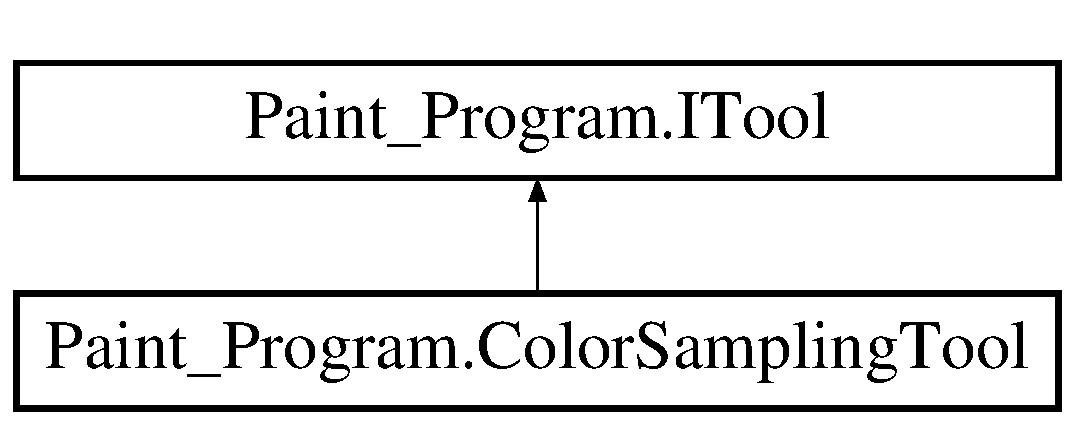
\includegraphics[height=2.000000cm]{class_paint___program_1_1_color_sampling_tool}
\end{center}
\end{figure}
\subsection*{Public Member Functions}
\begin{DoxyCompactItemize}
\item 
\mbox{\hyperlink{class_paint___program_1_1_color_sampling_tool_afaa3610c8758b8e047064b860472d1c9}{Color\+Sampling\+Tool}} ()
\item 
void \mbox{\hyperlink{class_paint___program_1_1_color_sampling_tool_ae6d5a44df3a4394f7da352d1170bea54}{Init}} ()
\item 
Bitmap \mbox{\hyperlink{class_paint___program_1_1_color_sampling_tool_a1824a80560c1dcfedfe12a326f0eae9c}{get\+Canvas}} ()
\item 
string \mbox{\hyperlink{class_paint___program_1_1_color_sampling_tool_a319d9e67417e473d0f76b8cafc1d7c2b}{Get\+Tool\+Icon\+Path}} ()
\item 
void \mbox{\hyperlink{class_paint___program_1_1_color_sampling_tool_a511da95eb2072dc913d8053ba405fb2a}{On\+Mouse\+Down}} (object sender, Mouse\+Event\+Args e)
\item 
void \mbox{\hyperlink{class_paint___program_1_1_color_sampling_tool_a509ae51233092f2722e44301897ee085}{On\+Mouse\+Move}} (object sender, Mouse\+Event\+Args e)
\item 
void \mbox{\hyperlink{class_paint___program_1_1_color_sampling_tool_a3365d954290cfb30d73c8a7c50fa7b72}{On\+Mouse\+Up}} (object sender, Mouse\+Event\+Args e)
\item 
bool \mbox{\hyperlink{class_paint___program_1_1_color_sampling_tool_a9ee3268dc9b5e8f36696055519a78a4c}{is\+Initalized}} ()
\item 
Bitmap \mbox{\hyperlink{class_paint___program_1_1_color_sampling_tool_aa0e2ac4d50f9a46c0d83a226e9e701c8}{Get\+Tool\+Layer}} ()
\item 
bool \mbox{\hyperlink{class_paint___program_1_1_color_sampling_tool_a68b28bfa791d073d5042b925261b6417}{Requires\+Layer\+Data}} ()
\item 
void \mbox{\hyperlink{class_paint___program_1_1_color_sampling_tool_a7f795564ca0d4df4287b2fb9a11891f4}{Set\+Layer\+Data}} (Bitmap bit)
\item 
string \mbox{\hyperlink{class_paint___program_1_1_color_sampling_tool_a6d26407d4a5040f66c417c7ccaf75793}{Get\+Tool\+Tip}} ()
\item 
void \mbox{\hyperlink{class_paint___program_1_1_color_sampling_tool_a0f2d672005a62b9ac04889c7a14cfcd0}{Update\+Interface\+Layer}} ()
\end{DoxyCompactItemize}
\subsection*{Private Attributes}
\begin{DoxyCompactItemize}
\item 
Graphics \mbox{\hyperlink{class_paint___program_1_1_color_sampling_tool_a0e4873b76a158efcfe923e488ad263a8}{graphics}}
\item 
int \mbox{\hyperlink{class_paint___program_1_1_color_sampling_tool_a49225951211d3ec7e1a476cab018d365}{width}}
\item 
int \mbox{\hyperlink{class_paint___program_1_1_color_sampling_tool_a62c3dd721f6b2a4feac63a3ae8428867}{height}}
\item 
bool \mbox{\hyperlink{class_paint___program_1_1_color_sampling_tool_a9ccea4c70e5aa59fa159694e0e3068c3}{b\+Active}}
\item 
bool \mbox{\hyperlink{class_paint___program_1_1_color_sampling_tool_a576ddeb6ab1d6d358dd88a171862bccb}{b\+Mouse\+Down}}
\item 
bool \mbox{\hyperlink{class_paint___program_1_1_color_sampling_tool_ad168d5e0845269f7639d736945502870}{b\+Init}}
\end{DoxyCompactItemize}


\subsection{Constructor \& Destructor Documentation}
\mbox{\Hypertarget{class_paint___program_1_1_color_sampling_tool_afaa3610c8758b8e047064b860472d1c9}\label{class_paint___program_1_1_color_sampling_tool_afaa3610c8758b8e047064b860472d1c9}} 
\index{Paint\+\_\+\+Program\+::\+Color\+Sampling\+Tool@{Paint\+\_\+\+Program\+::\+Color\+Sampling\+Tool}!Color\+Sampling\+Tool@{Color\+Sampling\+Tool}}
\index{Color\+Sampling\+Tool@{Color\+Sampling\+Tool}!Paint\+\_\+\+Program\+::\+Color\+Sampling\+Tool@{Paint\+\_\+\+Program\+::\+Color\+Sampling\+Tool}}
\subsubsection{\texorpdfstring{Color\+Sampling\+Tool()}{ColorSamplingTool()}}
{\footnotesize\ttfamily Paint\+\_\+\+Program.\+Color\+Sampling\+Tool.\+Color\+Sampling\+Tool (\begin{DoxyParamCaption}{ }\end{DoxyParamCaption})\hspace{0.3cm}{\ttfamily [inline]}}



\subsection{Member Function Documentation}
\mbox{\Hypertarget{class_paint___program_1_1_color_sampling_tool_a1824a80560c1dcfedfe12a326f0eae9c}\label{class_paint___program_1_1_color_sampling_tool_a1824a80560c1dcfedfe12a326f0eae9c}} 
\index{Paint\+\_\+\+Program\+::\+Color\+Sampling\+Tool@{Paint\+\_\+\+Program\+::\+Color\+Sampling\+Tool}!get\+Canvas@{get\+Canvas}}
\index{get\+Canvas@{get\+Canvas}!Paint\+\_\+\+Program\+::\+Color\+Sampling\+Tool@{Paint\+\_\+\+Program\+::\+Color\+Sampling\+Tool}}
\subsubsection{\texorpdfstring{get\+Canvas()}{getCanvas()}}
{\footnotesize\ttfamily Bitmap Paint\+\_\+\+Program.\+Color\+Sampling\+Tool.\+get\+Canvas (\begin{DoxyParamCaption}{ }\end{DoxyParamCaption})\hspace{0.3cm}{\ttfamily [inline]}}

\mbox{\Hypertarget{class_paint___program_1_1_color_sampling_tool_a319d9e67417e473d0f76b8cafc1d7c2b}\label{class_paint___program_1_1_color_sampling_tool_a319d9e67417e473d0f76b8cafc1d7c2b}} 
\index{Paint\+\_\+\+Program\+::\+Color\+Sampling\+Tool@{Paint\+\_\+\+Program\+::\+Color\+Sampling\+Tool}!Get\+Tool\+Icon\+Path@{Get\+Tool\+Icon\+Path}}
\index{Get\+Tool\+Icon\+Path@{Get\+Tool\+Icon\+Path}!Paint\+\_\+\+Program\+::\+Color\+Sampling\+Tool@{Paint\+\_\+\+Program\+::\+Color\+Sampling\+Tool}}
\subsubsection{\texorpdfstring{Get\+Tool\+Icon\+Path()}{GetToolIconPath()}}
{\footnotesize\ttfamily string Paint\+\_\+\+Program.\+Color\+Sampling\+Tool.\+Get\+Tool\+Icon\+Path (\begin{DoxyParamCaption}{ }\end{DoxyParamCaption})\hspace{0.3cm}{\ttfamily [inline]}}



Implements \mbox{\hyperlink{interface_paint___program_1_1_i_tool_aa057d2f99c59d7bec0215dcad2da1b72}{Paint\+\_\+\+Program.\+I\+Tool}}.

\mbox{\Hypertarget{class_paint___program_1_1_color_sampling_tool_aa0e2ac4d50f9a46c0d83a226e9e701c8}\label{class_paint___program_1_1_color_sampling_tool_aa0e2ac4d50f9a46c0d83a226e9e701c8}} 
\index{Paint\+\_\+\+Program\+::\+Color\+Sampling\+Tool@{Paint\+\_\+\+Program\+::\+Color\+Sampling\+Tool}!Get\+Tool\+Layer@{Get\+Tool\+Layer}}
\index{Get\+Tool\+Layer@{Get\+Tool\+Layer}!Paint\+\_\+\+Program\+::\+Color\+Sampling\+Tool@{Paint\+\_\+\+Program\+::\+Color\+Sampling\+Tool}}
\subsubsection{\texorpdfstring{Get\+Tool\+Layer()}{GetToolLayer()}}
{\footnotesize\ttfamily Bitmap Paint\+\_\+\+Program.\+Color\+Sampling\+Tool.\+Get\+Tool\+Layer (\begin{DoxyParamCaption}{ }\end{DoxyParamCaption})\hspace{0.3cm}{\ttfamily [inline]}}



Implements \mbox{\hyperlink{interface_paint___program_1_1_i_tool_a9b057905515f42a988c166a6a40318e0}{Paint\+\_\+\+Program.\+I\+Tool}}.

\mbox{\Hypertarget{class_paint___program_1_1_color_sampling_tool_a6d26407d4a5040f66c417c7ccaf75793}\label{class_paint___program_1_1_color_sampling_tool_a6d26407d4a5040f66c417c7ccaf75793}} 
\index{Paint\+\_\+\+Program\+::\+Color\+Sampling\+Tool@{Paint\+\_\+\+Program\+::\+Color\+Sampling\+Tool}!Get\+Tool\+Tip@{Get\+Tool\+Tip}}
\index{Get\+Tool\+Tip@{Get\+Tool\+Tip}!Paint\+\_\+\+Program\+::\+Color\+Sampling\+Tool@{Paint\+\_\+\+Program\+::\+Color\+Sampling\+Tool}}
\subsubsection{\texorpdfstring{Get\+Tool\+Tip()}{GetToolTip()}}
{\footnotesize\ttfamily string Paint\+\_\+\+Program.\+Color\+Sampling\+Tool.\+Get\+Tool\+Tip (\begin{DoxyParamCaption}{ }\end{DoxyParamCaption})\hspace{0.3cm}{\ttfamily [inline]}}



Implements \mbox{\hyperlink{interface_paint___program_1_1_i_tool_ac11f1591587144b6e74f5767bbf1df56}{Paint\+\_\+\+Program.\+I\+Tool}}.

\mbox{\Hypertarget{class_paint___program_1_1_color_sampling_tool_ae6d5a44df3a4394f7da352d1170bea54}\label{class_paint___program_1_1_color_sampling_tool_ae6d5a44df3a4394f7da352d1170bea54}} 
\index{Paint\+\_\+\+Program\+::\+Color\+Sampling\+Tool@{Paint\+\_\+\+Program\+::\+Color\+Sampling\+Tool}!Init@{Init}}
\index{Init@{Init}!Paint\+\_\+\+Program\+::\+Color\+Sampling\+Tool@{Paint\+\_\+\+Program\+::\+Color\+Sampling\+Tool}}
\subsubsection{\texorpdfstring{Init()}{Init()}}
{\footnotesize\ttfamily void Paint\+\_\+\+Program.\+Color\+Sampling\+Tool.\+Init (\begin{DoxyParamCaption}{ }\end{DoxyParamCaption})\hspace{0.3cm}{\ttfamily [inline]}}



Implements \mbox{\hyperlink{interface_paint___program_1_1_i_tool_af823123a30fbda34e24e907243241046}{Paint\+\_\+\+Program.\+I\+Tool}}.

\mbox{\Hypertarget{class_paint___program_1_1_color_sampling_tool_a9ee3268dc9b5e8f36696055519a78a4c}\label{class_paint___program_1_1_color_sampling_tool_a9ee3268dc9b5e8f36696055519a78a4c}} 
\index{Paint\+\_\+\+Program\+::\+Color\+Sampling\+Tool@{Paint\+\_\+\+Program\+::\+Color\+Sampling\+Tool}!is\+Initalized@{is\+Initalized}}
\index{is\+Initalized@{is\+Initalized}!Paint\+\_\+\+Program\+::\+Color\+Sampling\+Tool@{Paint\+\_\+\+Program\+::\+Color\+Sampling\+Tool}}
\subsubsection{\texorpdfstring{is\+Initalized()}{isInitalized()}}
{\footnotesize\ttfamily bool Paint\+\_\+\+Program.\+Color\+Sampling\+Tool.\+is\+Initalized (\begin{DoxyParamCaption}{ }\end{DoxyParamCaption})\hspace{0.3cm}{\ttfamily [inline]}}



Implements \mbox{\hyperlink{interface_paint___program_1_1_i_tool_a951b844bcbf47a6c306104fa86be7a5d}{Paint\+\_\+\+Program.\+I\+Tool}}.

\mbox{\Hypertarget{class_paint___program_1_1_color_sampling_tool_a511da95eb2072dc913d8053ba405fb2a}\label{class_paint___program_1_1_color_sampling_tool_a511da95eb2072dc913d8053ba405fb2a}} 
\index{Paint\+\_\+\+Program\+::\+Color\+Sampling\+Tool@{Paint\+\_\+\+Program\+::\+Color\+Sampling\+Tool}!On\+Mouse\+Down@{On\+Mouse\+Down}}
\index{On\+Mouse\+Down@{On\+Mouse\+Down}!Paint\+\_\+\+Program\+::\+Color\+Sampling\+Tool@{Paint\+\_\+\+Program\+::\+Color\+Sampling\+Tool}}
\subsubsection{\texorpdfstring{On\+Mouse\+Down()}{OnMouseDown()}}
{\footnotesize\ttfamily void Paint\+\_\+\+Program.\+Color\+Sampling\+Tool.\+On\+Mouse\+Down (\begin{DoxyParamCaption}\item[{object}]{sender,  }\item[{Mouse\+Event\+Args}]{e }\end{DoxyParamCaption})\hspace{0.3cm}{\ttfamily [inline]}}



Implements \mbox{\hyperlink{interface_paint___program_1_1_i_tool_a73d8797f4f2b1e0d8efe8aadcd44e840}{Paint\+\_\+\+Program.\+I\+Tool}}.

\mbox{\Hypertarget{class_paint___program_1_1_color_sampling_tool_a509ae51233092f2722e44301897ee085}\label{class_paint___program_1_1_color_sampling_tool_a509ae51233092f2722e44301897ee085}} 
\index{Paint\+\_\+\+Program\+::\+Color\+Sampling\+Tool@{Paint\+\_\+\+Program\+::\+Color\+Sampling\+Tool}!On\+Mouse\+Move@{On\+Mouse\+Move}}
\index{On\+Mouse\+Move@{On\+Mouse\+Move}!Paint\+\_\+\+Program\+::\+Color\+Sampling\+Tool@{Paint\+\_\+\+Program\+::\+Color\+Sampling\+Tool}}
\subsubsection{\texorpdfstring{On\+Mouse\+Move()}{OnMouseMove()}}
{\footnotesize\ttfamily void Paint\+\_\+\+Program.\+Color\+Sampling\+Tool.\+On\+Mouse\+Move (\begin{DoxyParamCaption}\item[{object}]{sender,  }\item[{Mouse\+Event\+Args}]{e }\end{DoxyParamCaption})\hspace{0.3cm}{\ttfamily [inline]}}



Implements \mbox{\hyperlink{interface_paint___program_1_1_i_tool_a6a1cbe840b5cfc8a9b9463cc21590845}{Paint\+\_\+\+Program.\+I\+Tool}}.

\mbox{\Hypertarget{class_paint___program_1_1_color_sampling_tool_a3365d954290cfb30d73c8a7c50fa7b72}\label{class_paint___program_1_1_color_sampling_tool_a3365d954290cfb30d73c8a7c50fa7b72}} 
\index{Paint\+\_\+\+Program\+::\+Color\+Sampling\+Tool@{Paint\+\_\+\+Program\+::\+Color\+Sampling\+Tool}!On\+Mouse\+Up@{On\+Mouse\+Up}}
\index{On\+Mouse\+Up@{On\+Mouse\+Up}!Paint\+\_\+\+Program\+::\+Color\+Sampling\+Tool@{Paint\+\_\+\+Program\+::\+Color\+Sampling\+Tool}}
\subsubsection{\texorpdfstring{On\+Mouse\+Up()}{OnMouseUp()}}
{\footnotesize\ttfamily void Paint\+\_\+\+Program.\+Color\+Sampling\+Tool.\+On\+Mouse\+Up (\begin{DoxyParamCaption}\item[{object}]{sender,  }\item[{Mouse\+Event\+Args}]{e }\end{DoxyParamCaption})\hspace{0.3cm}{\ttfamily [inline]}}



Implements \mbox{\hyperlink{interface_paint___program_1_1_i_tool_a47984c2879213022f1684c07f7bba73e}{Paint\+\_\+\+Program.\+I\+Tool}}.

\mbox{\Hypertarget{class_paint___program_1_1_color_sampling_tool_a68b28bfa791d073d5042b925261b6417}\label{class_paint___program_1_1_color_sampling_tool_a68b28bfa791d073d5042b925261b6417}} 
\index{Paint\+\_\+\+Program\+::\+Color\+Sampling\+Tool@{Paint\+\_\+\+Program\+::\+Color\+Sampling\+Tool}!Requires\+Layer\+Data@{Requires\+Layer\+Data}}
\index{Requires\+Layer\+Data@{Requires\+Layer\+Data}!Paint\+\_\+\+Program\+::\+Color\+Sampling\+Tool@{Paint\+\_\+\+Program\+::\+Color\+Sampling\+Tool}}
\subsubsection{\texorpdfstring{Requires\+Layer\+Data()}{RequiresLayerData()}}
{\footnotesize\ttfamily bool Paint\+\_\+\+Program.\+Color\+Sampling\+Tool.\+Requires\+Layer\+Data (\begin{DoxyParamCaption}{ }\end{DoxyParamCaption})\hspace{0.3cm}{\ttfamily [inline]}}



Implements \mbox{\hyperlink{interface_paint___program_1_1_i_tool_a6d45b6c48da8130ae41db3a66cdaef9a}{Paint\+\_\+\+Program.\+I\+Tool}}.

\mbox{\Hypertarget{class_paint___program_1_1_color_sampling_tool_a7f795564ca0d4df4287b2fb9a11891f4}\label{class_paint___program_1_1_color_sampling_tool_a7f795564ca0d4df4287b2fb9a11891f4}} 
\index{Paint\+\_\+\+Program\+::\+Color\+Sampling\+Tool@{Paint\+\_\+\+Program\+::\+Color\+Sampling\+Tool}!Set\+Layer\+Data@{Set\+Layer\+Data}}
\index{Set\+Layer\+Data@{Set\+Layer\+Data}!Paint\+\_\+\+Program\+::\+Color\+Sampling\+Tool@{Paint\+\_\+\+Program\+::\+Color\+Sampling\+Tool}}
\subsubsection{\texorpdfstring{Set\+Layer\+Data()}{SetLayerData()}}
{\footnotesize\ttfamily void Paint\+\_\+\+Program.\+Color\+Sampling\+Tool.\+Set\+Layer\+Data (\begin{DoxyParamCaption}\item[{Bitmap}]{bit }\end{DoxyParamCaption})\hspace{0.3cm}{\ttfamily [inline]}}



Implements \mbox{\hyperlink{interface_paint___program_1_1_i_tool_a2d3e63715dfe04075d27dacf367d1633}{Paint\+\_\+\+Program.\+I\+Tool}}.

\mbox{\Hypertarget{class_paint___program_1_1_color_sampling_tool_a0f2d672005a62b9ac04889c7a14cfcd0}\label{class_paint___program_1_1_color_sampling_tool_a0f2d672005a62b9ac04889c7a14cfcd0}} 
\index{Paint\+\_\+\+Program\+::\+Color\+Sampling\+Tool@{Paint\+\_\+\+Program\+::\+Color\+Sampling\+Tool}!Update\+Interface\+Layer@{Update\+Interface\+Layer}}
\index{Update\+Interface\+Layer@{Update\+Interface\+Layer}!Paint\+\_\+\+Program\+::\+Color\+Sampling\+Tool@{Paint\+\_\+\+Program\+::\+Color\+Sampling\+Tool}}
\subsubsection{\texorpdfstring{Update\+Interface\+Layer()}{UpdateInterfaceLayer()}}
{\footnotesize\ttfamily void Paint\+\_\+\+Program.\+Color\+Sampling\+Tool.\+Update\+Interface\+Layer (\begin{DoxyParamCaption}{ }\end{DoxyParamCaption})\hspace{0.3cm}{\ttfamily [inline]}}



Implements \mbox{\hyperlink{interface_paint___program_1_1_i_tool_a36db75d29e88dfd739f658633c40e955}{Paint\+\_\+\+Program.\+I\+Tool}}.



\subsection{Member Data Documentation}
\mbox{\Hypertarget{class_paint___program_1_1_color_sampling_tool_a9ccea4c70e5aa59fa159694e0e3068c3}\label{class_paint___program_1_1_color_sampling_tool_a9ccea4c70e5aa59fa159694e0e3068c3}} 
\index{Paint\+\_\+\+Program\+::\+Color\+Sampling\+Tool@{Paint\+\_\+\+Program\+::\+Color\+Sampling\+Tool}!b\+Active@{b\+Active}}
\index{b\+Active@{b\+Active}!Paint\+\_\+\+Program\+::\+Color\+Sampling\+Tool@{Paint\+\_\+\+Program\+::\+Color\+Sampling\+Tool}}
\subsubsection{\texorpdfstring{b\+Active}{bActive}}
{\footnotesize\ttfamily bool Paint\+\_\+\+Program.\+Color\+Sampling\+Tool.\+b\+Active\hspace{0.3cm}{\ttfamily [private]}}

\mbox{\Hypertarget{class_paint___program_1_1_color_sampling_tool_ad168d5e0845269f7639d736945502870}\label{class_paint___program_1_1_color_sampling_tool_ad168d5e0845269f7639d736945502870}} 
\index{Paint\+\_\+\+Program\+::\+Color\+Sampling\+Tool@{Paint\+\_\+\+Program\+::\+Color\+Sampling\+Tool}!b\+Init@{b\+Init}}
\index{b\+Init@{b\+Init}!Paint\+\_\+\+Program\+::\+Color\+Sampling\+Tool@{Paint\+\_\+\+Program\+::\+Color\+Sampling\+Tool}}
\subsubsection{\texorpdfstring{b\+Init}{bInit}}
{\footnotesize\ttfamily bool Paint\+\_\+\+Program.\+Color\+Sampling\+Tool.\+b\+Init\hspace{0.3cm}{\ttfamily [private]}}

\mbox{\Hypertarget{class_paint___program_1_1_color_sampling_tool_a576ddeb6ab1d6d358dd88a171862bccb}\label{class_paint___program_1_1_color_sampling_tool_a576ddeb6ab1d6d358dd88a171862bccb}} 
\index{Paint\+\_\+\+Program\+::\+Color\+Sampling\+Tool@{Paint\+\_\+\+Program\+::\+Color\+Sampling\+Tool}!b\+Mouse\+Down@{b\+Mouse\+Down}}
\index{b\+Mouse\+Down@{b\+Mouse\+Down}!Paint\+\_\+\+Program\+::\+Color\+Sampling\+Tool@{Paint\+\_\+\+Program\+::\+Color\+Sampling\+Tool}}
\subsubsection{\texorpdfstring{b\+Mouse\+Down}{bMouseDown}}
{\footnotesize\ttfamily bool Paint\+\_\+\+Program.\+Color\+Sampling\+Tool.\+b\+Mouse\+Down\hspace{0.3cm}{\ttfamily [private]}}

\mbox{\Hypertarget{class_paint___program_1_1_color_sampling_tool_a0e4873b76a158efcfe923e488ad263a8}\label{class_paint___program_1_1_color_sampling_tool_a0e4873b76a158efcfe923e488ad263a8}} 
\index{Paint\+\_\+\+Program\+::\+Color\+Sampling\+Tool@{Paint\+\_\+\+Program\+::\+Color\+Sampling\+Tool}!graphics@{graphics}}
\index{graphics@{graphics}!Paint\+\_\+\+Program\+::\+Color\+Sampling\+Tool@{Paint\+\_\+\+Program\+::\+Color\+Sampling\+Tool}}
\subsubsection{\texorpdfstring{graphics}{graphics}}
{\footnotesize\ttfamily Graphics Paint\+\_\+\+Program.\+Color\+Sampling\+Tool.\+graphics\hspace{0.3cm}{\ttfamily [private]}}

\mbox{\Hypertarget{class_paint___program_1_1_color_sampling_tool_a62c3dd721f6b2a4feac63a3ae8428867}\label{class_paint___program_1_1_color_sampling_tool_a62c3dd721f6b2a4feac63a3ae8428867}} 
\index{Paint\+\_\+\+Program\+::\+Color\+Sampling\+Tool@{Paint\+\_\+\+Program\+::\+Color\+Sampling\+Tool}!height@{height}}
\index{height@{height}!Paint\+\_\+\+Program\+::\+Color\+Sampling\+Tool@{Paint\+\_\+\+Program\+::\+Color\+Sampling\+Tool}}
\subsubsection{\texorpdfstring{height}{height}}
{\footnotesize\ttfamily int Paint\+\_\+\+Program.\+Color\+Sampling\+Tool.\+height\hspace{0.3cm}{\ttfamily [private]}}

\mbox{\Hypertarget{class_paint___program_1_1_color_sampling_tool_a49225951211d3ec7e1a476cab018d365}\label{class_paint___program_1_1_color_sampling_tool_a49225951211d3ec7e1a476cab018d365}} 
\index{Paint\+\_\+\+Program\+::\+Color\+Sampling\+Tool@{Paint\+\_\+\+Program\+::\+Color\+Sampling\+Tool}!width@{width}}
\index{width@{width}!Paint\+\_\+\+Program\+::\+Color\+Sampling\+Tool@{Paint\+\_\+\+Program\+::\+Color\+Sampling\+Tool}}
\subsubsection{\texorpdfstring{width}{width}}
{\footnotesize\ttfamily int Paint\+\_\+\+Program.\+Color\+Sampling\+Tool.\+width\hspace{0.3cm}{\ttfamily [private]}}



The documentation for this class was generated from the following file\+:\begin{DoxyCompactItemize}
\item 
Paint Program/\mbox{\hyperlink{_color_sampling_tool_8cs}{Color\+Sampling\+Tool.\+cs}}\end{DoxyCompactItemize}

\hypertarget{class_wintab_d_n_1_1_c_wintab_context}{}\section{Wintab\+D\+N.\+C\+Wintab\+Context Class Reference}
\label{class_wintab_d_n_1_1_c_wintab_context}\index{Wintab\+D\+N.\+C\+Wintab\+Context@{Wintab\+D\+N.\+C\+Wintab\+Context}}


Class to support access to Wintab context management.  


\subsection*{Public Member Functions}
\begin{DoxyCompactItemize}
\item 
\mbox{\hyperlink{class_wintab_d_n_1_1_c_wintab_context_ae2ce09949d3d633790254555f9db2d49}{C\+Wintab\+Context}} ()
\begin{DoxyCompactList}\small\item\em Default constructor sets all data bits to be captured. \end{DoxyCompactList}\item 
\mbox{\hyperlink{class_wintab_d_n_1_1_h_c_t_x}{H\+C\+TX}} \mbox{\hyperlink{class_wintab_d_n_1_1_c_wintab_context_a4bb06f01ce05bcac01ed611ea7d241d8}{Open}} (\mbox{\hyperlink{struct_wintab_d_n_1_1_h_w_n_d}{H\+W\+ND}} hwnd\+\_\+I, bool enable\+\_\+I)
\begin{DoxyCompactList}\small\item\em Open a Wintab context to the specified hwnd. \end{DoxyCompactList}\item 
bool \mbox{\hyperlink{class_wintab_d_n_1_1_c_wintab_context_a1522d857d00373971e9c0e010ae9e756}{Open}} ()
\begin{DoxyCompactList}\small\item\em Open a Wintab context that will send packet events to a message window. \end{DoxyCompactList}\item 
bool \mbox{\hyperlink{class_wintab_d_n_1_1_c_wintab_context_a53d935082727bc049f9d817363e6200f}{Close}} ()
\begin{DoxyCompactList}\small\item\em Close the context for this object. \end{DoxyCompactList}\item 
bool \mbox{\hyperlink{class_wintab_d_n_1_1_c_wintab_context_a580c1e6691c4c58c8d54d429e7d7ebd8}{Enable}} (bool enable\+\_\+I)
\begin{DoxyCompactList}\small\item\em Enable/disable this Wintab context. \end{DoxyCompactList}\item 
bool \mbox{\hyperlink{class_wintab_d_n_1_1_c_wintab_context_a26240e1cdf96ad7859a8fae08a41e412}{Set\+Overlap\+Order}} (bool to\+Top\+\_\+I)
\begin{DoxyCompactList}\small\item\em Sends a tablet context to the top or bottom of the order of overlapping tablet contexts \end{DoxyCompactList}\end{DoxyCompactItemize}
\subsection*{Properties}
\begin{DoxyCompactItemize}
\item 
\mbox{\hyperlink{struct_wintab_d_n_1_1_wintab_log_context}{Wintab\+Log\+Context}} \mbox{\hyperlink{class_wintab_d_n_1_1_c_wintab_context_ad1aaf328b7c7aeb2b98e8c4e167047b6}{Log\+Context}}\hspace{0.3cm}{\ttfamily  \mbox{[}get, set\mbox{]}}
\begin{DoxyCompactList}\small\item\em Logical Wintab context managed by this object. ~\newline
\end{DoxyCompactList}\item 
\mbox{\hyperlink{class_wintab_d_n_1_1_h_c_t_x}{H\+C\+TX}} \mbox{\hyperlink{class_wintab_d_n_1_1_c_wintab_context_ad4709db10fbf92aa19dcdf0c19c53415}{H\+Ctx}}\hspace{0.3cm}{\ttfamily  \mbox{[}get\mbox{]}}
\begin{DoxyCompactList}\small\item\em Handle (identifier) used to identify this context. \end{DoxyCompactList}\item 
string \mbox{\hyperlink{class_wintab_d_n_1_1_c_wintab_context_a275c652af6e326a3b8750ae5ea047237}{Name}}\hspace{0.3cm}{\ttfamily  \mbox{[}get, set\mbox{]}}
\begin{DoxyCompactList}\small\item\em Get/\+Set context name. \end{DoxyCompactList}\item 
U\+Int32 \mbox{\hyperlink{class_wintab_d_n_1_1_c_wintab_context_a3e5d1e938f9bd00d82474b670292b5a7}{Options}}\hspace{0.3cm}{\ttfamily  \mbox{[}get, set\mbox{]}}
\begin{DoxyCompactList}\small\item\em Specifies options for the context. These options can be combined by using the bitwise OR operator. The lc\+Options field can be any combination of the values defined in E\+C\+T\+X\+Option\+Values. \end{DoxyCompactList}\item 
U\+Int32 \mbox{\hyperlink{class_wintab_d_n_1_1_c_wintab_context_a25169d39580b4d7a30d7feb05c1872d5}{Status}}\hspace{0.3cm}{\ttfamily  \mbox{[}get, set\mbox{]}}
\begin{DoxyCompactList}\small\item\em Specifies current status conditions for the context. These conditions can be combined by using the bitwise OR operator. The lc\+Status field can be any combination of the values defined in E\+C\+T\+X\+Status\+Values. \end{DoxyCompactList}\item 
U\+Int32 \mbox{\hyperlink{class_wintab_d_n_1_1_c_wintab_context_ab05bc9afc19654c5495adfb60efdc06d}{Locks}}\hspace{0.3cm}{\ttfamily  \mbox{[}get, set\mbox{]}}
\begin{DoxyCompactList}\small\item\em Specifies which attributes of the context the application wishes to be locked. Lock conditions specify attributes of the context that cannot be changed once the context has been opened (calls to W\+T\+Config will have no effect on the locked attributes). The lock conditions can be combined by using the bitwise OR operator. The lc\+Locks field can be any combination of the values defined in E\+C\+T\+X\+Lock\+Values. Locks can only be changed by the task or process that owns the context. \end{DoxyCompactList}\item 
U\+Int32 \mbox{\hyperlink{class_wintab_d_n_1_1_c_wintab_context_a074fcb0607df8048600719c8875b12a7}{Msg\+Base}}\hspace{0.3cm}{\ttfamily  \mbox{[}get, set\mbox{]}}
\begin{DoxyCompactList}\small\item\em Specifies the range of message numbers that will be used for reporting the activity of the context. \end{DoxyCompactList}\item 
U\+Int32 \mbox{\hyperlink{class_wintab_d_n_1_1_c_wintab_context_a1f56c63dab67a86ba44b53bce0bc882a}{Device}}\hspace{0.3cm}{\ttfamily  \mbox{[}get, set\mbox{]}}
\begin{DoxyCompactList}\small\item\em Specifies the device whose input the context processes. \end{DoxyCompactList}\item 
U\+Int32 \mbox{\hyperlink{class_wintab_d_n_1_1_c_wintab_context_a20f3b1ba020637ac525e1a2f0a67011f}{Pkt\+Rate}}\hspace{0.3cm}{\ttfamily  \mbox{[}get, set\mbox{]}}
\begin{DoxyCompactList}\small\item\em Specifies the desired packet report rate in Hertz. Once the con-\/text is opened, this field will contain the actual report rate. \end{DoxyCompactList}\item 
\mbox{\hyperlink{class_wintab_d_n_1_1_w_t_p_k_t}{W\+T\+P\+KT}} \mbox{\hyperlink{class_wintab_d_n_1_1_c_wintab_context_a3da21ad3b21239b8463f54a83f7f1bb8}{Pkt\+Data}}\hspace{0.3cm}{\ttfamily  \mbox{[}get, set\mbox{]}}
\begin{DoxyCompactList}\small\item\em Specifies which optional data items will be in packets returned from the context. Requesting unsupported data items will cause \mbox{\hyperlink{class_wintab_d_n_1_1_c_wintab_context_a1522d857d00373971e9c0e010ae9e756}{Open()}} to fail. \end{DoxyCompactList}\item 
\mbox{\hyperlink{class_wintab_d_n_1_1_w_t_p_k_t}{W\+T\+P\+KT}} \mbox{\hyperlink{class_wintab_d_n_1_1_c_wintab_context_a05489816378ed5052a3e0e6a8a517d7b}{Pkt\+Mode}}\hspace{0.3cm}{\ttfamily  \mbox{[}get, set\mbox{]}}
\begin{DoxyCompactList}\small\item\em Specifies whether the packet data items will be returned in absolute or relative mode. If the item\textquotesingle{}s bit is set in this field, the item will be returned in relative mode. Bits in this field for items not selected in the Pkt\+Data property will be ignored. Bits for data items that only allow one mode (such as the packet identifier) will also be ignored. ~\newline
\end{DoxyCompactList}\item 
\mbox{\hyperlink{class_wintab_d_n_1_1_w_t_p_k_t}{W\+T\+P\+KT}} \mbox{\hyperlink{class_wintab_d_n_1_1_c_wintab_context_a76772f28304fd4f8e4c511e7b65bdd59}{Move\+Mask}}\hspace{0.3cm}{\ttfamily  \mbox{[}get, set\mbox{]}}
\begin{DoxyCompactList}\small\item\em Specifies which packet data items can generate move events in the context. Bits for items that are not part of the packet definition in the Pkt\+Data property will be ignored. The bits for buttons, time stamp, and the packet identifier will also be ignored. In the case of overlapping contexts, movement events for data items not selected in this field may be processed by underlying contexts. \end{DoxyCompactList}\item 
U\+Int32 \mbox{\hyperlink{class_wintab_d_n_1_1_c_wintab_context_a972a0b1d0634fc580aa65b8943af3905}{Btn\+Dn\+Mask}}\hspace{0.3cm}{\ttfamily  \mbox{[}get, set\mbox{]}}
\begin{DoxyCompactList}\small\item\em Specifies the buttons for which button press events will be processed in the context. In the case of overlapping contexts, button press events for buttons that are not selected in this field may be processed by underlying contexts. \end{DoxyCompactList}\item 
U\+Int32 \mbox{\hyperlink{class_wintab_d_n_1_1_c_wintab_context_af90630abd6dc8926709bbf875744de8c}{Btn\+Up\+Mask}}\hspace{0.3cm}{\ttfamily  \mbox{[}get, set\mbox{]}}
\begin{DoxyCompactList}\small\item\em Specifies the buttons for which button release events will be processed in the context. In the case of overlapping contexts, button release events for buttons that are not selected in this field may be processed by underlying contexts. If both press and release events are selected for a button (see the Btn\+Dn\+Mask property), then the interface will cause the context to implicitly capture all tablet events while the button is down. In this case, events occurring outside the context will be clipped to the context and processed as if they had occurred in the context. When the button is released, the context will receive the button release event, and then event processing will return to normal. \end{DoxyCompactList}\item 
Int32 \mbox{\hyperlink{class_wintab_d_n_1_1_c_wintab_context_a326fb62231cb2f9b783cb29a6716b6b7}{In\+OrgX}}\hspace{0.3cm}{\ttfamily  \mbox{[}get, set\mbox{]}}
\begin{DoxyCompactList}\small\item\em Specifies the X origin of the context\textquotesingle{}s input area in the tablet\textquotesingle{}s native coordinates. Value is clipped to the tablet native coordinate space when the context is opened or modified. \end{DoxyCompactList}\item 
Int32 \mbox{\hyperlink{class_wintab_d_n_1_1_c_wintab_context_a0f480b34eb30bf42edd2adf565572ae3}{In\+OrgY}}\hspace{0.3cm}{\ttfamily  \mbox{[}get, set\mbox{]}}
\begin{DoxyCompactList}\small\item\em Specifies the Y origin of the context\textquotesingle{}s input area in the tablet\textquotesingle{}s native coordinates. Value is clipped to the tablet native coordinate space when the context is opened or modified. \end{DoxyCompactList}\item 
Int32 \mbox{\hyperlink{class_wintab_d_n_1_1_c_wintab_context_afe123e2d48ea3c171c2b040dd512cda6}{In\+OrgZ}}\hspace{0.3cm}{\ttfamily  \mbox{[}get, set\mbox{]}}
\begin{DoxyCompactList}\small\item\em Specifies the Z origin of the context\textquotesingle{}s input area in the tablet\textquotesingle{}s native coordinates. Value is clipped to the tablet native coordinate space when the context is opened or modified. \end{DoxyCompactList}\item 
Int32 \mbox{\hyperlink{class_wintab_d_n_1_1_c_wintab_context_a8f33e05910bcde9fe611f32a986a1ea5}{In\+ExtX}}\hspace{0.3cm}{\ttfamily  \mbox{[}get, set\mbox{]}}
\begin{DoxyCompactList}\small\item\em Specifies the X extent of the context\textquotesingle{}s input area in the tablet\textquotesingle{}s native coordinates. Value is clipped to the tablet native coordinate space when the context is opened or modified. \end{DoxyCompactList}\item 
Int32 \mbox{\hyperlink{class_wintab_d_n_1_1_c_wintab_context_abb73e61691a4b2480b7997b73202b63b}{In\+ExtY}}\hspace{0.3cm}{\ttfamily  \mbox{[}get, set\mbox{]}}
\begin{DoxyCompactList}\small\item\em Specifies the Y extent of the context\textquotesingle{}s input area in the tablet\textquotesingle{}s native coordinates. Value is clipped to the tablet native coordinate space when the context is opened or modified. \end{DoxyCompactList}\item 
Int32 \mbox{\hyperlink{class_wintab_d_n_1_1_c_wintab_context_a8d699ca76769679eca827b033e4f5fde}{In\+ExtZ}}\hspace{0.3cm}{\ttfamily  \mbox{[}get, set\mbox{]}}
\begin{DoxyCompactList}\small\item\em Specifies the Z extent of the context\textquotesingle{}s input area in the tablet\textquotesingle{}s native coordinates. Value is clipped to the tablet native coordinate space when the context is opened or modified. \end{DoxyCompactList}\item 
Int32 \mbox{\hyperlink{class_wintab_d_n_1_1_c_wintab_context_a93f133c38a24202d1b3b7396893ed7fd}{Out\+OrgX}}\hspace{0.3cm}{\ttfamily  \mbox{[}get, set\mbox{]}}
\begin{DoxyCompactList}\small\item\em Specifies the X origin of the context\textquotesingle{}s output area in context output coordinates. Value is used in coordinate scaling for absolute mode only. \end{DoxyCompactList}\item 
Int32 \mbox{\hyperlink{class_wintab_d_n_1_1_c_wintab_context_a5d27ca1711aa3f176519a1484936972b}{Out\+OrgY}}\hspace{0.3cm}{\ttfamily  \mbox{[}get, set\mbox{]}}
\begin{DoxyCompactList}\small\item\em Specifies the Y origin of the context\textquotesingle{}s output area in context output coordinates. Value is used in coordinate scaling for absolute mode only. \end{DoxyCompactList}\item 
Int32 \mbox{\hyperlink{class_wintab_d_n_1_1_c_wintab_context_aee6840f04cc34b466e683d9892e82648}{Out\+OrgZ}}\hspace{0.3cm}{\ttfamily  \mbox{[}get, set\mbox{]}}
\begin{DoxyCompactList}\small\item\em Specifies the Z origin of the context\textquotesingle{}s output area in context output coordinates. Value is used in coordinate scaling for absolute mode only. \end{DoxyCompactList}\item 
Int32 \mbox{\hyperlink{class_wintab_d_n_1_1_c_wintab_context_af911044cb67b004b35cca63883d598ae}{Out\+ExtX}}\hspace{0.3cm}{\ttfamily  \mbox{[}get, set\mbox{]}}
\begin{DoxyCompactList}\small\item\em Specifies the X extent of the context\textquotesingle{}s output area in context output coordinates. Value is used in coordinate scaling for absolute mode only. \end{DoxyCompactList}\item 
Int32 \mbox{\hyperlink{class_wintab_d_n_1_1_c_wintab_context_aeb9155dbf8f387cfa2a38679b5af45a3}{Out\+ExtY}}\hspace{0.3cm}{\ttfamily  \mbox{[}get, set\mbox{]}}
\begin{DoxyCompactList}\small\item\em Specifies the Y extent of the context\textquotesingle{}s output area in context output coordinates. Value is used in coordinate scaling for absolute mode only. \end{DoxyCompactList}\item 
Int32 \mbox{\hyperlink{class_wintab_d_n_1_1_c_wintab_context_a02c9755f5d0ccefef8aa8728136b3c7d}{Out\+ExtZ}}\hspace{0.3cm}{\ttfamily  \mbox{[}get, set\mbox{]}}
\begin{DoxyCompactList}\small\item\em Specifies the Z extent of the context\textquotesingle{}s output area in context output coordinates. Value is used in coordinate scaling for absolute mode only. \end{DoxyCompactList}\item 
\mbox{\hyperlink{class_wintab_d_n_1_1_f_i_x32}{F\+I\+X32}} \mbox{\hyperlink{class_wintab_d_n_1_1_c_wintab_context_ab5cff8c2a8dbecad852fb2fb7d4a31d4}{SensX}}\hspace{0.3cm}{\ttfamily  \mbox{[}get, set\mbox{]}}
\begin{DoxyCompactList}\small\item\em Specifies the relative-\/mode sensitivity factor for the x axis. \end{DoxyCompactList}\item 
\mbox{\hyperlink{class_wintab_d_n_1_1_f_i_x32}{F\+I\+X32}} \mbox{\hyperlink{class_wintab_d_n_1_1_c_wintab_context_ac35412cff3ea7455fedd6e2e38cd65e5}{SensY}}\hspace{0.3cm}{\ttfamily  \mbox{[}get, set\mbox{]}}
\begin{DoxyCompactList}\small\item\em Specifies the relative-\/mode sensitivity factor for the y axis. \end{DoxyCompactList}\item 
\mbox{\hyperlink{class_wintab_d_n_1_1_f_i_x32}{F\+I\+X32}} \mbox{\hyperlink{class_wintab_d_n_1_1_c_wintab_context_a4908c82cd430554df3ca0e1268ee3af9}{SensZ}}\hspace{0.3cm}{\ttfamily  \mbox{[}get, set\mbox{]}}
\begin{DoxyCompactList}\small\item\em Specifies the relative-\/mode sensitivity factor for the Z axis. \end{DoxyCompactList}\item 
bool \mbox{\hyperlink{class_wintab_d_n_1_1_c_wintab_context_a50763a15570f18f433580630dfa7fe8a}{Sys\+Mode}}\hspace{0.3cm}{\ttfamily  \mbox{[}get, set\mbox{]}}
\begin{DoxyCompactList}\small\item\em Specifies the system cursor tracking mode. Zero specifies absolute; non-\/zero means relative. \end{DoxyCompactList}\item 
Int32 \mbox{\hyperlink{class_wintab_d_n_1_1_c_wintab_context_a14ba5470dacaafe10618a3d4cd0931bd}{Sys\+OrgX}}\hspace{0.3cm}{\ttfamily  \mbox{[}get, set\mbox{]}}
\begin{DoxyCompactList}\small\item\em Specifies the X origin of the screen mapping area for system cursor tracking, in screen coordinates. \end{DoxyCompactList}\item 
Int32 \mbox{\hyperlink{class_wintab_d_n_1_1_c_wintab_context_ab630649b89e1029b4ded69f815cf9947}{Sys\+OrgY}}\hspace{0.3cm}{\ttfamily  \mbox{[}get, set\mbox{]}}
\begin{DoxyCompactList}\small\item\em Specifies the Y origin of the screen mapping area for system cursor tracking, in screen coordinates. \end{DoxyCompactList}\item 
Int32 \mbox{\hyperlink{class_wintab_d_n_1_1_c_wintab_context_af7bb13537c0ce3d915309bcc4de86bb3}{Sys\+ExtX}}\hspace{0.3cm}{\ttfamily  \mbox{[}get, set\mbox{]}}
\begin{DoxyCompactList}\small\item\em Specifies the X extent of the screen mapping area for system cursor tracking, in screen coordinates. \end{DoxyCompactList}\item 
Int32 \mbox{\hyperlink{class_wintab_d_n_1_1_c_wintab_context_abcafe640181563d36f23c87433f485a5}{Sys\+ExtY}}\hspace{0.3cm}{\ttfamily  \mbox{[}get, set\mbox{]}}
\begin{DoxyCompactList}\small\item\em Specifies the Y extent of the screen mapping area for system cursor tracking, in screen coordinates. \end{DoxyCompactList}\item 
\mbox{\hyperlink{class_wintab_d_n_1_1_f_i_x32}{F\+I\+X32}} \mbox{\hyperlink{class_wintab_d_n_1_1_c_wintab_context_ae4188eab9083490c471951381961d6a8}{Sys\+SensX}}\hspace{0.3cm}{\ttfamily  \mbox{[}get, set\mbox{]}}
\begin{DoxyCompactList}\small\item\em Specifies the system-\/cursor relative-\/mode sensitivity factor for the x axis. \end{DoxyCompactList}\item 
\mbox{\hyperlink{class_wintab_d_n_1_1_f_i_x32}{F\+I\+X32}} \mbox{\hyperlink{class_wintab_d_n_1_1_c_wintab_context_ab1c31c691d5659eb3bde3c999b62d5b6}{Sys\+SensY}}\hspace{0.3cm}{\ttfamily  \mbox{[}get, set\mbox{]}}
\begin{DoxyCompactList}\small\item\em Specifies the system-\/cursor relative-\/mode sensitivity factor for the y axis. \end{DoxyCompactList}\end{DoxyCompactItemize}
\subsection*{Private Attributes}
\begin{DoxyCompactItemize}
\item 
const bool \mbox{\hyperlink{class_wintab_d_n_1_1_c_wintab_context_aff540bf7703bf6e96bae3d5bfc3eaaa7}{D\+I\+S\+P\+L\+A\+Y\+\_\+\+M\+E\+S\+S\+A\+G\+E\+\_\+\+B\+O\+X\+ES}} = false
\item 
\mbox{\hyperlink{struct_wintab_d_n_1_1_wintab_log_context}{Wintab\+Log\+Context}} \mbox{\hyperlink{class_wintab_d_n_1_1_c_wintab_context_a076aee1ffdce4966d7f4b46acd39d501}{m\+\_\+log\+Context}} = new \mbox{\hyperlink{struct_wintab_d_n_1_1_wintab_log_context}{Wintab\+Log\+Context}}()
\item 
\mbox{\hyperlink{class_wintab_d_n_1_1_h_c_t_x}{H\+C\+TX}} \mbox{\hyperlink{class_wintab_d_n_1_1_c_wintab_context_ab31f2970a3e0658878f4716dbe2387cd}{m\+\_\+h\+C\+TX}} = 0
\end{DoxyCompactItemize}


\subsection{Detailed Description}
Class to support access to Wintab context management. 



\subsection{Constructor \& Destructor Documentation}
\mbox{\Hypertarget{class_wintab_d_n_1_1_c_wintab_context_ae2ce09949d3d633790254555f9db2d49}\label{class_wintab_d_n_1_1_c_wintab_context_ae2ce09949d3d633790254555f9db2d49}} 
\index{Wintab\+D\+N\+::\+C\+Wintab\+Context@{Wintab\+D\+N\+::\+C\+Wintab\+Context}!C\+Wintab\+Context@{C\+Wintab\+Context}}
\index{C\+Wintab\+Context@{C\+Wintab\+Context}!Wintab\+D\+N\+::\+C\+Wintab\+Context@{Wintab\+D\+N\+::\+C\+Wintab\+Context}}
\subsubsection{\texorpdfstring{C\+Wintab\+Context()}{CWintabContext()}}
{\footnotesize\ttfamily Wintab\+D\+N.\+C\+Wintab\+Context.\+C\+Wintab\+Context (\begin{DoxyParamCaption}{ }\end{DoxyParamCaption})\hspace{0.3cm}{\ttfamily [inline]}}



Default constructor sets all data bits to be captured. 



\subsection{Member Function Documentation}
\mbox{\Hypertarget{class_wintab_d_n_1_1_c_wintab_context_a53d935082727bc049f9d817363e6200f}\label{class_wintab_d_n_1_1_c_wintab_context_a53d935082727bc049f9d817363e6200f}} 
\index{Wintab\+D\+N\+::\+C\+Wintab\+Context@{Wintab\+D\+N\+::\+C\+Wintab\+Context}!Close@{Close}}
\index{Close@{Close}!Wintab\+D\+N\+::\+C\+Wintab\+Context@{Wintab\+D\+N\+::\+C\+Wintab\+Context}}
\subsubsection{\texorpdfstring{Close()}{Close()}}
{\footnotesize\ttfamily bool Wintab\+D\+N.\+C\+Wintab\+Context.\+Close (\begin{DoxyParamCaption}{ }\end{DoxyParamCaption})\hspace{0.3cm}{\ttfamily [inline]}}



Close the context for this object. 

\begin{DoxyReturn}{Returns}
true if context successfully closed
\end{DoxyReturn}
\mbox{\Hypertarget{class_wintab_d_n_1_1_c_wintab_context_a580c1e6691c4c58c8d54d429e7d7ebd8}\label{class_wintab_d_n_1_1_c_wintab_context_a580c1e6691c4c58c8d54d429e7d7ebd8}} 
\index{Wintab\+D\+N\+::\+C\+Wintab\+Context@{Wintab\+D\+N\+::\+C\+Wintab\+Context}!Enable@{Enable}}
\index{Enable@{Enable}!Wintab\+D\+N\+::\+C\+Wintab\+Context@{Wintab\+D\+N\+::\+C\+Wintab\+Context}}
\subsubsection{\texorpdfstring{Enable()}{Enable()}}
{\footnotesize\ttfamily bool Wintab\+D\+N.\+C\+Wintab\+Context.\+Enable (\begin{DoxyParamCaption}\item[{bool}]{enable\+\_\+I }\end{DoxyParamCaption})\hspace{0.3cm}{\ttfamily [inline]}}



Enable/disable this Wintab context. 


\begin{DoxyParams}{Parameters}
{\em enable\+\_\+I} & true = enable\\
\hline
\end{DoxyParams}
\begin{DoxyReturn}{Returns}
Returns true if completed successfully
\end{DoxyReturn}
\mbox{\Hypertarget{class_wintab_d_n_1_1_c_wintab_context_a4bb06f01ce05bcac01ed611ea7d241d8}\label{class_wintab_d_n_1_1_c_wintab_context_a4bb06f01ce05bcac01ed611ea7d241d8}} 
\index{Wintab\+D\+N\+::\+C\+Wintab\+Context@{Wintab\+D\+N\+::\+C\+Wintab\+Context}!Open@{Open}}
\index{Open@{Open}!Wintab\+D\+N\+::\+C\+Wintab\+Context@{Wintab\+D\+N\+::\+C\+Wintab\+Context}}
\subsubsection{\texorpdfstring{Open()}{Open()}\hspace{0.1cm}{\footnotesize\ttfamily [1/2]}}
{\footnotesize\ttfamily \mbox{\hyperlink{class_wintab_d_n_1_1_h_c_t_x}{H\+C\+TX}} Wintab\+D\+N.\+C\+Wintab\+Context.\+Open (\begin{DoxyParamCaption}\item[{\mbox{\hyperlink{struct_wintab_d_n_1_1_h_w_n_d}{H\+W\+ND}}}]{hwnd\+\_\+I,  }\item[{bool}]{enable\+\_\+I }\end{DoxyParamCaption})\hspace{0.3cm}{\ttfamily [inline]}}



Open a Wintab context to the specified hwnd. 


\begin{DoxyParams}{Parameters}
{\em hwnd\+\_\+I} & parent window for the context\\
\hline
{\em enable\+\_\+I} & true to enable, false to disable\\
\hline
\end{DoxyParams}
\begin{DoxyReturn}{Returns}
Returns non-\/zero context handle if successful.
\end{DoxyReturn}
\mbox{\Hypertarget{class_wintab_d_n_1_1_c_wintab_context_a1522d857d00373971e9c0e010ae9e756}\label{class_wintab_d_n_1_1_c_wintab_context_a1522d857d00373971e9c0e010ae9e756}} 
\index{Wintab\+D\+N\+::\+C\+Wintab\+Context@{Wintab\+D\+N\+::\+C\+Wintab\+Context}!Open@{Open}}
\index{Open@{Open}!Wintab\+D\+N\+::\+C\+Wintab\+Context@{Wintab\+D\+N\+::\+C\+Wintab\+Context}}
\subsubsection{\texorpdfstring{Open()}{Open()}\hspace{0.1cm}{\footnotesize\ttfamily [2/2]}}
{\footnotesize\ttfamily bool Wintab\+D\+N.\+C\+Wintab\+Context.\+Open (\begin{DoxyParamCaption}{ }\end{DoxyParamCaption})\hspace{0.3cm}{\ttfamily [inline]}}



Open a Wintab context that will send packet events to a message window. 

\begin{DoxyReturn}{Returns}
Returns true if successful.
\end{DoxyReturn}
\mbox{\Hypertarget{class_wintab_d_n_1_1_c_wintab_context_a26240e1cdf96ad7859a8fae08a41e412}\label{class_wintab_d_n_1_1_c_wintab_context_a26240e1cdf96ad7859a8fae08a41e412}} 
\index{Wintab\+D\+N\+::\+C\+Wintab\+Context@{Wintab\+D\+N\+::\+C\+Wintab\+Context}!Set\+Overlap\+Order@{Set\+Overlap\+Order}}
\index{Set\+Overlap\+Order@{Set\+Overlap\+Order}!Wintab\+D\+N\+::\+C\+Wintab\+Context@{Wintab\+D\+N\+::\+C\+Wintab\+Context}}
\subsubsection{\texorpdfstring{Set\+Overlap\+Order()}{SetOverlapOrder()}}
{\footnotesize\ttfamily bool Wintab\+D\+N.\+C\+Wintab\+Context.\+Set\+Overlap\+Order (\begin{DoxyParamCaption}\item[{bool}]{to\+Top\+\_\+I }\end{DoxyParamCaption})\hspace{0.3cm}{\ttfamily [inline]}}



Sends a tablet context to the top or bottom of the order of overlapping tablet contexts 


\begin{DoxyParams}{Parameters}
{\em to\+Top\+\_\+I} & true = send tablet to top of order\\
\hline
\end{DoxyParams}
\begin{DoxyReturn}{Returns}
Returns true if successsful
\end{DoxyReturn}


\subsection{Member Data Documentation}
\mbox{\Hypertarget{class_wintab_d_n_1_1_c_wintab_context_aff540bf7703bf6e96bae3d5bfc3eaaa7}\label{class_wintab_d_n_1_1_c_wintab_context_aff540bf7703bf6e96bae3d5bfc3eaaa7}} 
\index{Wintab\+D\+N\+::\+C\+Wintab\+Context@{Wintab\+D\+N\+::\+C\+Wintab\+Context}!D\+I\+S\+P\+L\+A\+Y\+\_\+\+M\+E\+S\+S\+A\+G\+E\+\_\+\+B\+O\+X\+ES@{D\+I\+S\+P\+L\+A\+Y\+\_\+\+M\+E\+S\+S\+A\+G\+E\+\_\+\+B\+O\+X\+ES}}
\index{D\+I\+S\+P\+L\+A\+Y\+\_\+\+M\+E\+S\+S\+A\+G\+E\+\_\+\+B\+O\+X\+ES@{D\+I\+S\+P\+L\+A\+Y\+\_\+\+M\+E\+S\+S\+A\+G\+E\+\_\+\+B\+O\+X\+ES}!Wintab\+D\+N\+::\+C\+Wintab\+Context@{Wintab\+D\+N\+::\+C\+Wintab\+Context}}
\subsubsection{\texorpdfstring{D\+I\+S\+P\+L\+A\+Y\+\_\+\+M\+E\+S\+S\+A\+G\+E\+\_\+\+B\+O\+X\+ES}{DISPLAY\_MESSAGE\_BOXES}}
{\footnotesize\ttfamily const bool Wintab\+D\+N.\+C\+Wintab\+Context.\+D\+I\+S\+P\+L\+A\+Y\+\_\+\+M\+E\+S\+S\+A\+G\+E\+\_\+\+B\+O\+X\+ES = false\hspace{0.3cm}{\ttfamily [private]}}

\mbox{\Hypertarget{class_wintab_d_n_1_1_c_wintab_context_ab31f2970a3e0658878f4716dbe2387cd}\label{class_wintab_d_n_1_1_c_wintab_context_ab31f2970a3e0658878f4716dbe2387cd}} 
\index{Wintab\+D\+N\+::\+C\+Wintab\+Context@{Wintab\+D\+N\+::\+C\+Wintab\+Context}!m\+\_\+h\+C\+TX@{m\+\_\+h\+C\+TX}}
\index{m\+\_\+h\+C\+TX@{m\+\_\+h\+C\+TX}!Wintab\+D\+N\+::\+C\+Wintab\+Context@{Wintab\+D\+N\+::\+C\+Wintab\+Context}}
\subsubsection{\texorpdfstring{m\+\_\+h\+C\+TX}{m\_hCTX}}
{\footnotesize\ttfamily \mbox{\hyperlink{class_wintab_d_n_1_1_h_c_t_x}{H\+C\+TX}} Wintab\+D\+N.\+C\+Wintab\+Context.\+m\+\_\+h\+C\+TX = 0\hspace{0.3cm}{\ttfamily [private]}}

\mbox{\Hypertarget{class_wintab_d_n_1_1_c_wintab_context_a076aee1ffdce4966d7f4b46acd39d501}\label{class_wintab_d_n_1_1_c_wintab_context_a076aee1ffdce4966d7f4b46acd39d501}} 
\index{Wintab\+D\+N\+::\+C\+Wintab\+Context@{Wintab\+D\+N\+::\+C\+Wintab\+Context}!m\+\_\+log\+Context@{m\+\_\+log\+Context}}
\index{m\+\_\+log\+Context@{m\+\_\+log\+Context}!Wintab\+D\+N\+::\+C\+Wintab\+Context@{Wintab\+D\+N\+::\+C\+Wintab\+Context}}
\subsubsection{\texorpdfstring{m\+\_\+log\+Context}{m\_logContext}}
{\footnotesize\ttfamily \mbox{\hyperlink{struct_wintab_d_n_1_1_wintab_log_context}{Wintab\+Log\+Context}} Wintab\+D\+N.\+C\+Wintab\+Context.\+m\+\_\+log\+Context = new \mbox{\hyperlink{struct_wintab_d_n_1_1_wintab_log_context}{Wintab\+Log\+Context}}()\hspace{0.3cm}{\ttfamily [private]}}



\subsection{Property Documentation}
\mbox{\Hypertarget{class_wintab_d_n_1_1_c_wintab_context_a972a0b1d0634fc580aa65b8943af3905}\label{class_wintab_d_n_1_1_c_wintab_context_a972a0b1d0634fc580aa65b8943af3905}} 
\index{Wintab\+D\+N\+::\+C\+Wintab\+Context@{Wintab\+D\+N\+::\+C\+Wintab\+Context}!Btn\+Dn\+Mask@{Btn\+Dn\+Mask}}
\index{Btn\+Dn\+Mask@{Btn\+Dn\+Mask}!Wintab\+D\+N\+::\+C\+Wintab\+Context@{Wintab\+D\+N\+::\+C\+Wintab\+Context}}
\subsubsection{\texorpdfstring{Btn\+Dn\+Mask}{BtnDnMask}}
{\footnotesize\ttfamily U\+Int32 Wintab\+D\+N.\+C\+Wintab\+Context.\+Btn\+Dn\+Mask\hspace{0.3cm}{\ttfamily [get]}, {\ttfamily [set]}}



Specifies the buttons for which button press events will be processed in the context. In the case of overlapping contexts, button press events for buttons that are not selected in this field may be processed by underlying contexts. 

\mbox{\Hypertarget{class_wintab_d_n_1_1_c_wintab_context_af90630abd6dc8926709bbf875744de8c}\label{class_wintab_d_n_1_1_c_wintab_context_af90630abd6dc8926709bbf875744de8c}} 
\index{Wintab\+D\+N\+::\+C\+Wintab\+Context@{Wintab\+D\+N\+::\+C\+Wintab\+Context}!Btn\+Up\+Mask@{Btn\+Up\+Mask}}
\index{Btn\+Up\+Mask@{Btn\+Up\+Mask}!Wintab\+D\+N\+::\+C\+Wintab\+Context@{Wintab\+D\+N\+::\+C\+Wintab\+Context}}
\subsubsection{\texorpdfstring{Btn\+Up\+Mask}{BtnUpMask}}
{\footnotesize\ttfamily U\+Int32 Wintab\+D\+N.\+C\+Wintab\+Context.\+Btn\+Up\+Mask\hspace{0.3cm}{\ttfamily [get]}, {\ttfamily [set]}}



Specifies the buttons for which button release events will be processed in the context. In the case of overlapping contexts, button release events for buttons that are not selected in this field may be processed by underlying contexts. If both press and release events are selected for a button (see the Btn\+Dn\+Mask property), then the interface will cause the context to implicitly capture all tablet events while the button is down. In this case, events occurring outside the context will be clipped to the context and processed as if they had occurred in the context. When the button is released, the context will receive the button release event, and then event processing will return to normal. 

\mbox{\Hypertarget{class_wintab_d_n_1_1_c_wintab_context_a1f56c63dab67a86ba44b53bce0bc882a}\label{class_wintab_d_n_1_1_c_wintab_context_a1f56c63dab67a86ba44b53bce0bc882a}} 
\index{Wintab\+D\+N\+::\+C\+Wintab\+Context@{Wintab\+D\+N\+::\+C\+Wintab\+Context}!Device@{Device}}
\index{Device@{Device}!Wintab\+D\+N\+::\+C\+Wintab\+Context@{Wintab\+D\+N\+::\+C\+Wintab\+Context}}
\subsubsection{\texorpdfstring{Device}{Device}}
{\footnotesize\ttfamily U\+Int32 Wintab\+D\+N.\+C\+Wintab\+Context.\+Device\hspace{0.3cm}{\ttfamily [get]}, {\ttfamily [set]}}



Specifies the device whose input the context processes. 

\mbox{\Hypertarget{class_wintab_d_n_1_1_c_wintab_context_ad4709db10fbf92aa19dcdf0c19c53415}\label{class_wintab_d_n_1_1_c_wintab_context_ad4709db10fbf92aa19dcdf0c19c53415}} 
\index{Wintab\+D\+N\+::\+C\+Wintab\+Context@{Wintab\+D\+N\+::\+C\+Wintab\+Context}!H\+Ctx@{H\+Ctx}}
\index{H\+Ctx@{H\+Ctx}!Wintab\+D\+N\+::\+C\+Wintab\+Context@{Wintab\+D\+N\+::\+C\+Wintab\+Context}}
\subsubsection{\texorpdfstring{H\+Ctx}{HCtx}}
{\footnotesize\ttfamily \mbox{\hyperlink{class_wintab_d_n_1_1_h_c_t_x}{H\+C\+TX}} Wintab\+D\+N.\+C\+Wintab\+Context.\+H\+Ctx\hspace{0.3cm}{\ttfamily [get]}}



Handle (identifier) used to identify this context. 

\mbox{\Hypertarget{class_wintab_d_n_1_1_c_wintab_context_a8f33e05910bcde9fe611f32a986a1ea5}\label{class_wintab_d_n_1_1_c_wintab_context_a8f33e05910bcde9fe611f32a986a1ea5}} 
\index{Wintab\+D\+N\+::\+C\+Wintab\+Context@{Wintab\+D\+N\+::\+C\+Wintab\+Context}!In\+ExtX@{In\+ExtX}}
\index{In\+ExtX@{In\+ExtX}!Wintab\+D\+N\+::\+C\+Wintab\+Context@{Wintab\+D\+N\+::\+C\+Wintab\+Context}}
\subsubsection{\texorpdfstring{In\+ExtX}{InExtX}}
{\footnotesize\ttfamily Int32 Wintab\+D\+N.\+C\+Wintab\+Context.\+In\+ExtX\hspace{0.3cm}{\ttfamily [get]}, {\ttfamily [set]}}



Specifies the X extent of the context\textquotesingle{}s input area in the tablet\textquotesingle{}s native coordinates. Value is clipped to the tablet native coordinate space when the context is opened or modified. 

\mbox{\Hypertarget{class_wintab_d_n_1_1_c_wintab_context_abb73e61691a4b2480b7997b73202b63b}\label{class_wintab_d_n_1_1_c_wintab_context_abb73e61691a4b2480b7997b73202b63b}} 
\index{Wintab\+D\+N\+::\+C\+Wintab\+Context@{Wintab\+D\+N\+::\+C\+Wintab\+Context}!In\+ExtY@{In\+ExtY}}
\index{In\+ExtY@{In\+ExtY}!Wintab\+D\+N\+::\+C\+Wintab\+Context@{Wintab\+D\+N\+::\+C\+Wintab\+Context}}
\subsubsection{\texorpdfstring{In\+ExtY}{InExtY}}
{\footnotesize\ttfamily Int32 Wintab\+D\+N.\+C\+Wintab\+Context.\+In\+ExtY\hspace{0.3cm}{\ttfamily [get]}, {\ttfamily [set]}}



Specifies the Y extent of the context\textquotesingle{}s input area in the tablet\textquotesingle{}s native coordinates. Value is clipped to the tablet native coordinate space when the context is opened or modified. 

\mbox{\Hypertarget{class_wintab_d_n_1_1_c_wintab_context_a8d699ca76769679eca827b033e4f5fde}\label{class_wintab_d_n_1_1_c_wintab_context_a8d699ca76769679eca827b033e4f5fde}} 
\index{Wintab\+D\+N\+::\+C\+Wintab\+Context@{Wintab\+D\+N\+::\+C\+Wintab\+Context}!In\+ExtZ@{In\+ExtZ}}
\index{In\+ExtZ@{In\+ExtZ}!Wintab\+D\+N\+::\+C\+Wintab\+Context@{Wintab\+D\+N\+::\+C\+Wintab\+Context}}
\subsubsection{\texorpdfstring{In\+ExtZ}{InExtZ}}
{\footnotesize\ttfamily Int32 Wintab\+D\+N.\+C\+Wintab\+Context.\+In\+ExtZ\hspace{0.3cm}{\ttfamily [get]}, {\ttfamily [set]}}



Specifies the Z extent of the context\textquotesingle{}s input area in the tablet\textquotesingle{}s native coordinates. Value is clipped to the tablet native coordinate space when the context is opened or modified. 

\mbox{\Hypertarget{class_wintab_d_n_1_1_c_wintab_context_a326fb62231cb2f9b783cb29a6716b6b7}\label{class_wintab_d_n_1_1_c_wintab_context_a326fb62231cb2f9b783cb29a6716b6b7}} 
\index{Wintab\+D\+N\+::\+C\+Wintab\+Context@{Wintab\+D\+N\+::\+C\+Wintab\+Context}!In\+OrgX@{In\+OrgX}}
\index{In\+OrgX@{In\+OrgX}!Wintab\+D\+N\+::\+C\+Wintab\+Context@{Wintab\+D\+N\+::\+C\+Wintab\+Context}}
\subsubsection{\texorpdfstring{In\+OrgX}{InOrgX}}
{\footnotesize\ttfamily Int32 Wintab\+D\+N.\+C\+Wintab\+Context.\+In\+OrgX\hspace{0.3cm}{\ttfamily [get]}, {\ttfamily [set]}}



Specifies the X origin of the context\textquotesingle{}s input area in the tablet\textquotesingle{}s native coordinates. Value is clipped to the tablet native coordinate space when the context is opened or modified. 

\mbox{\Hypertarget{class_wintab_d_n_1_1_c_wintab_context_a0f480b34eb30bf42edd2adf565572ae3}\label{class_wintab_d_n_1_1_c_wintab_context_a0f480b34eb30bf42edd2adf565572ae3}} 
\index{Wintab\+D\+N\+::\+C\+Wintab\+Context@{Wintab\+D\+N\+::\+C\+Wintab\+Context}!In\+OrgY@{In\+OrgY}}
\index{In\+OrgY@{In\+OrgY}!Wintab\+D\+N\+::\+C\+Wintab\+Context@{Wintab\+D\+N\+::\+C\+Wintab\+Context}}
\subsubsection{\texorpdfstring{In\+OrgY}{InOrgY}}
{\footnotesize\ttfamily Int32 Wintab\+D\+N.\+C\+Wintab\+Context.\+In\+OrgY\hspace{0.3cm}{\ttfamily [get]}, {\ttfamily [set]}}



Specifies the Y origin of the context\textquotesingle{}s input area in the tablet\textquotesingle{}s native coordinates. Value is clipped to the tablet native coordinate space when the context is opened or modified. 

\mbox{\Hypertarget{class_wintab_d_n_1_1_c_wintab_context_afe123e2d48ea3c171c2b040dd512cda6}\label{class_wintab_d_n_1_1_c_wintab_context_afe123e2d48ea3c171c2b040dd512cda6}} 
\index{Wintab\+D\+N\+::\+C\+Wintab\+Context@{Wintab\+D\+N\+::\+C\+Wintab\+Context}!In\+OrgZ@{In\+OrgZ}}
\index{In\+OrgZ@{In\+OrgZ}!Wintab\+D\+N\+::\+C\+Wintab\+Context@{Wintab\+D\+N\+::\+C\+Wintab\+Context}}
\subsubsection{\texorpdfstring{In\+OrgZ}{InOrgZ}}
{\footnotesize\ttfamily Int32 Wintab\+D\+N.\+C\+Wintab\+Context.\+In\+OrgZ\hspace{0.3cm}{\ttfamily [get]}, {\ttfamily [set]}}



Specifies the Z origin of the context\textquotesingle{}s input area in the tablet\textquotesingle{}s native coordinates. Value is clipped to the tablet native coordinate space when the context is opened or modified. 

\mbox{\Hypertarget{class_wintab_d_n_1_1_c_wintab_context_ab05bc9afc19654c5495adfb60efdc06d}\label{class_wintab_d_n_1_1_c_wintab_context_ab05bc9afc19654c5495adfb60efdc06d}} 
\index{Wintab\+D\+N\+::\+C\+Wintab\+Context@{Wintab\+D\+N\+::\+C\+Wintab\+Context}!Locks@{Locks}}
\index{Locks@{Locks}!Wintab\+D\+N\+::\+C\+Wintab\+Context@{Wintab\+D\+N\+::\+C\+Wintab\+Context}}
\subsubsection{\texorpdfstring{Locks}{Locks}}
{\footnotesize\ttfamily U\+Int32 Wintab\+D\+N.\+C\+Wintab\+Context.\+Locks\hspace{0.3cm}{\ttfamily [get]}, {\ttfamily [set]}}



Specifies which attributes of the context the application wishes to be locked. Lock conditions specify attributes of the context that cannot be changed once the context has been opened (calls to W\+T\+Config will have no effect on the locked attributes). The lock conditions can be combined by using the bitwise OR operator. The lc\+Locks field can be any combination of the values defined in E\+C\+T\+X\+Lock\+Values. Locks can only be changed by the task or process that owns the context. 

\mbox{\Hypertarget{class_wintab_d_n_1_1_c_wintab_context_ad1aaf328b7c7aeb2b98e8c4e167047b6}\label{class_wintab_d_n_1_1_c_wintab_context_ad1aaf328b7c7aeb2b98e8c4e167047b6}} 
\index{Wintab\+D\+N\+::\+C\+Wintab\+Context@{Wintab\+D\+N\+::\+C\+Wintab\+Context}!Log\+Context@{Log\+Context}}
\index{Log\+Context@{Log\+Context}!Wintab\+D\+N\+::\+C\+Wintab\+Context@{Wintab\+D\+N\+::\+C\+Wintab\+Context}}
\subsubsection{\texorpdfstring{Log\+Context}{LogContext}}
{\footnotesize\ttfamily \mbox{\hyperlink{struct_wintab_d_n_1_1_wintab_log_context}{Wintab\+Log\+Context}} Wintab\+D\+N.\+C\+Wintab\+Context.\+Log\+Context\hspace{0.3cm}{\ttfamily [get]}, {\ttfamily [set]}}



Logical Wintab context managed by this object. ~\newline


\mbox{\Hypertarget{class_wintab_d_n_1_1_c_wintab_context_a76772f28304fd4f8e4c511e7b65bdd59}\label{class_wintab_d_n_1_1_c_wintab_context_a76772f28304fd4f8e4c511e7b65bdd59}} 
\index{Wintab\+D\+N\+::\+C\+Wintab\+Context@{Wintab\+D\+N\+::\+C\+Wintab\+Context}!Move\+Mask@{Move\+Mask}}
\index{Move\+Mask@{Move\+Mask}!Wintab\+D\+N\+::\+C\+Wintab\+Context@{Wintab\+D\+N\+::\+C\+Wintab\+Context}}
\subsubsection{\texorpdfstring{Move\+Mask}{MoveMask}}
{\footnotesize\ttfamily \mbox{\hyperlink{class_wintab_d_n_1_1_w_t_p_k_t}{W\+T\+P\+KT}} Wintab\+D\+N.\+C\+Wintab\+Context.\+Move\+Mask\hspace{0.3cm}{\ttfamily [get]}, {\ttfamily [set]}}



Specifies which packet data items can generate move events in the context. Bits for items that are not part of the packet definition in the Pkt\+Data property will be ignored. The bits for buttons, time stamp, and the packet identifier will also be ignored. In the case of overlapping contexts, movement events for data items not selected in this field may be processed by underlying contexts. 

\mbox{\Hypertarget{class_wintab_d_n_1_1_c_wintab_context_a074fcb0607df8048600719c8875b12a7}\label{class_wintab_d_n_1_1_c_wintab_context_a074fcb0607df8048600719c8875b12a7}} 
\index{Wintab\+D\+N\+::\+C\+Wintab\+Context@{Wintab\+D\+N\+::\+C\+Wintab\+Context}!Msg\+Base@{Msg\+Base}}
\index{Msg\+Base@{Msg\+Base}!Wintab\+D\+N\+::\+C\+Wintab\+Context@{Wintab\+D\+N\+::\+C\+Wintab\+Context}}
\subsubsection{\texorpdfstring{Msg\+Base}{MsgBase}}
{\footnotesize\ttfamily U\+Int32 Wintab\+D\+N.\+C\+Wintab\+Context.\+Msg\+Base\hspace{0.3cm}{\ttfamily [get]}, {\ttfamily [set]}}



Specifies the range of message numbers that will be used for reporting the activity of the context. 

\mbox{\Hypertarget{class_wintab_d_n_1_1_c_wintab_context_a275c652af6e326a3b8750ae5ea047237}\label{class_wintab_d_n_1_1_c_wintab_context_a275c652af6e326a3b8750ae5ea047237}} 
\index{Wintab\+D\+N\+::\+C\+Wintab\+Context@{Wintab\+D\+N\+::\+C\+Wintab\+Context}!Name@{Name}}
\index{Name@{Name}!Wintab\+D\+N\+::\+C\+Wintab\+Context@{Wintab\+D\+N\+::\+C\+Wintab\+Context}}
\subsubsection{\texorpdfstring{Name}{Name}}
{\footnotesize\ttfamily string Wintab\+D\+N.\+C\+Wintab\+Context.\+Name\hspace{0.3cm}{\ttfamily [get]}, {\ttfamily [set]}}



Get/\+Set context name. 

\mbox{\Hypertarget{class_wintab_d_n_1_1_c_wintab_context_a3e5d1e938f9bd00d82474b670292b5a7}\label{class_wintab_d_n_1_1_c_wintab_context_a3e5d1e938f9bd00d82474b670292b5a7}} 
\index{Wintab\+D\+N\+::\+C\+Wintab\+Context@{Wintab\+D\+N\+::\+C\+Wintab\+Context}!Options@{Options}}
\index{Options@{Options}!Wintab\+D\+N\+::\+C\+Wintab\+Context@{Wintab\+D\+N\+::\+C\+Wintab\+Context}}
\subsubsection{\texorpdfstring{Options}{Options}}
{\footnotesize\ttfamily U\+Int32 Wintab\+D\+N.\+C\+Wintab\+Context.\+Options\hspace{0.3cm}{\ttfamily [get]}, {\ttfamily [set]}}



Specifies options for the context. These options can be combined by using the bitwise OR operator. The lc\+Options field can be any combination of the values defined in E\+C\+T\+X\+Option\+Values. 

\mbox{\Hypertarget{class_wintab_d_n_1_1_c_wintab_context_af911044cb67b004b35cca63883d598ae}\label{class_wintab_d_n_1_1_c_wintab_context_af911044cb67b004b35cca63883d598ae}} 
\index{Wintab\+D\+N\+::\+C\+Wintab\+Context@{Wintab\+D\+N\+::\+C\+Wintab\+Context}!Out\+ExtX@{Out\+ExtX}}
\index{Out\+ExtX@{Out\+ExtX}!Wintab\+D\+N\+::\+C\+Wintab\+Context@{Wintab\+D\+N\+::\+C\+Wintab\+Context}}
\subsubsection{\texorpdfstring{Out\+ExtX}{OutExtX}}
{\footnotesize\ttfamily Int32 Wintab\+D\+N.\+C\+Wintab\+Context.\+Out\+ExtX\hspace{0.3cm}{\ttfamily [get]}, {\ttfamily [set]}}



Specifies the X extent of the context\textquotesingle{}s output area in context output coordinates. Value is used in coordinate scaling for absolute mode only. 

\mbox{\Hypertarget{class_wintab_d_n_1_1_c_wintab_context_aeb9155dbf8f387cfa2a38679b5af45a3}\label{class_wintab_d_n_1_1_c_wintab_context_aeb9155dbf8f387cfa2a38679b5af45a3}} 
\index{Wintab\+D\+N\+::\+C\+Wintab\+Context@{Wintab\+D\+N\+::\+C\+Wintab\+Context}!Out\+ExtY@{Out\+ExtY}}
\index{Out\+ExtY@{Out\+ExtY}!Wintab\+D\+N\+::\+C\+Wintab\+Context@{Wintab\+D\+N\+::\+C\+Wintab\+Context}}
\subsubsection{\texorpdfstring{Out\+ExtY}{OutExtY}}
{\footnotesize\ttfamily Int32 Wintab\+D\+N.\+C\+Wintab\+Context.\+Out\+ExtY\hspace{0.3cm}{\ttfamily [get]}, {\ttfamily [set]}}



Specifies the Y extent of the context\textquotesingle{}s output area in context output coordinates. Value is used in coordinate scaling for absolute mode only. 

\mbox{\Hypertarget{class_wintab_d_n_1_1_c_wintab_context_a02c9755f5d0ccefef8aa8728136b3c7d}\label{class_wintab_d_n_1_1_c_wintab_context_a02c9755f5d0ccefef8aa8728136b3c7d}} 
\index{Wintab\+D\+N\+::\+C\+Wintab\+Context@{Wintab\+D\+N\+::\+C\+Wintab\+Context}!Out\+ExtZ@{Out\+ExtZ}}
\index{Out\+ExtZ@{Out\+ExtZ}!Wintab\+D\+N\+::\+C\+Wintab\+Context@{Wintab\+D\+N\+::\+C\+Wintab\+Context}}
\subsubsection{\texorpdfstring{Out\+ExtZ}{OutExtZ}}
{\footnotesize\ttfamily Int32 Wintab\+D\+N.\+C\+Wintab\+Context.\+Out\+ExtZ\hspace{0.3cm}{\ttfamily [get]}, {\ttfamily [set]}}



Specifies the Z extent of the context\textquotesingle{}s output area in context output coordinates. Value is used in coordinate scaling for absolute mode only. 

\mbox{\Hypertarget{class_wintab_d_n_1_1_c_wintab_context_a93f133c38a24202d1b3b7396893ed7fd}\label{class_wintab_d_n_1_1_c_wintab_context_a93f133c38a24202d1b3b7396893ed7fd}} 
\index{Wintab\+D\+N\+::\+C\+Wintab\+Context@{Wintab\+D\+N\+::\+C\+Wintab\+Context}!Out\+OrgX@{Out\+OrgX}}
\index{Out\+OrgX@{Out\+OrgX}!Wintab\+D\+N\+::\+C\+Wintab\+Context@{Wintab\+D\+N\+::\+C\+Wintab\+Context}}
\subsubsection{\texorpdfstring{Out\+OrgX}{OutOrgX}}
{\footnotesize\ttfamily Int32 Wintab\+D\+N.\+C\+Wintab\+Context.\+Out\+OrgX\hspace{0.3cm}{\ttfamily [get]}, {\ttfamily [set]}}



Specifies the X origin of the context\textquotesingle{}s output area in context output coordinates. Value is used in coordinate scaling for absolute mode only. 

\mbox{\Hypertarget{class_wintab_d_n_1_1_c_wintab_context_a5d27ca1711aa3f176519a1484936972b}\label{class_wintab_d_n_1_1_c_wintab_context_a5d27ca1711aa3f176519a1484936972b}} 
\index{Wintab\+D\+N\+::\+C\+Wintab\+Context@{Wintab\+D\+N\+::\+C\+Wintab\+Context}!Out\+OrgY@{Out\+OrgY}}
\index{Out\+OrgY@{Out\+OrgY}!Wintab\+D\+N\+::\+C\+Wintab\+Context@{Wintab\+D\+N\+::\+C\+Wintab\+Context}}
\subsubsection{\texorpdfstring{Out\+OrgY}{OutOrgY}}
{\footnotesize\ttfamily Int32 Wintab\+D\+N.\+C\+Wintab\+Context.\+Out\+OrgY\hspace{0.3cm}{\ttfamily [get]}, {\ttfamily [set]}}



Specifies the Y origin of the context\textquotesingle{}s output area in context output coordinates. Value is used in coordinate scaling for absolute mode only. 

\mbox{\Hypertarget{class_wintab_d_n_1_1_c_wintab_context_aee6840f04cc34b466e683d9892e82648}\label{class_wintab_d_n_1_1_c_wintab_context_aee6840f04cc34b466e683d9892e82648}} 
\index{Wintab\+D\+N\+::\+C\+Wintab\+Context@{Wintab\+D\+N\+::\+C\+Wintab\+Context}!Out\+OrgZ@{Out\+OrgZ}}
\index{Out\+OrgZ@{Out\+OrgZ}!Wintab\+D\+N\+::\+C\+Wintab\+Context@{Wintab\+D\+N\+::\+C\+Wintab\+Context}}
\subsubsection{\texorpdfstring{Out\+OrgZ}{OutOrgZ}}
{\footnotesize\ttfamily Int32 Wintab\+D\+N.\+C\+Wintab\+Context.\+Out\+OrgZ\hspace{0.3cm}{\ttfamily [get]}, {\ttfamily [set]}}



Specifies the Z origin of the context\textquotesingle{}s output area in context output coordinates. Value is used in coordinate scaling for absolute mode only. 

\mbox{\Hypertarget{class_wintab_d_n_1_1_c_wintab_context_a3da21ad3b21239b8463f54a83f7f1bb8}\label{class_wintab_d_n_1_1_c_wintab_context_a3da21ad3b21239b8463f54a83f7f1bb8}} 
\index{Wintab\+D\+N\+::\+C\+Wintab\+Context@{Wintab\+D\+N\+::\+C\+Wintab\+Context}!Pkt\+Data@{Pkt\+Data}}
\index{Pkt\+Data@{Pkt\+Data}!Wintab\+D\+N\+::\+C\+Wintab\+Context@{Wintab\+D\+N\+::\+C\+Wintab\+Context}}
\subsubsection{\texorpdfstring{Pkt\+Data}{PktData}}
{\footnotesize\ttfamily \mbox{\hyperlink{class_wintab_d_n_1_1_w_t_p_k_t}{W\+T\+P\+KT}} Wintab\+D\+N.\+C\+Wintab\+Context.\+Pkt\+Data\hspace{0.3cm}{\ttfamily [get]}, {\ttfamily [set]}}



Specifies which optional data items will be in packets returned from the context. Requesting unsupported data items will cause \mbox{\hyperlink{class_wintab_d_n_1_1_c_wintab_context_a1522d857d00373971e9c0e010ae9e756}{Open()}} to fail. 

\mbox{\Hypertarget{class_wintab_d_n_1_1_c_wintab_context_a05489816378ed5052a3e0e6a8a517d7b}\label{class_wintab_d_n_1_1_c_wintab_context_a05489816378ed5052a3e0e6a8a517d7b}} 
\index{Wintab\+D\+N\+::\+C\+Wintab\+Context@{Wintab\+D\+N\+::\+C\+Wintab\+Context}!Pkt\+Mode@{Pkt\+Mode}}
\index{Pkt\+Mode@{Pkt\+Mode}!Wintab\+D\+N\+::\+C\+Wintab\+Context@{Wintab\+D\+N\+::\+C\+Wintab\+Context}}
\subsubsection{\texorpdfstring{Pkt\+Mode}{PktMode}}
{\footnotesize\ttfamily \mbox{\hyperlink{class_wintab_d_n_1_1_w_t_p_k_t}{W\+T\+P\+KT}} Wintab\+D\+N.\+C\+Wintab\+Context.\+Pkt\+Mode\hspace{0.3cm}{\ttfamily [get]}, {\ttfamily [set]}}



Specifies whether the packet data items will be returned in absolute or relative mode. If the item\textquotesingle{}s bit is set in this field, the item will be returned in relative mode. Bits in this field for items not selected in the Pkt\+Data property will be ignored. Bits for data items that only allow one mode (such as the packet identifier) will also be ignored. ~\newline


\mbox{\Hypertarget{class_wintab_d_n_1_1_c_wintab_context_a20f3b1ba020637ac525e1a2f0a67011f}\label{class_wintab_d_n_1_1_c_wintab_context_a20f3b1ba020637ac525e1a2f0a67011f}} 
\index{Wintab\+D\+N\+::\+C\+Wintab\+Context@{Wintab\+D\+N\+::\+C\+Wintab\+Context}!Pkt\+Rate@{Pkt\+Rate}}
\index{Pkt\+Rate@{Pkt\+Rate}!Wintab\+D\+N\+::\+C\+Wintab\+Context@{Wintab\+D\+N\+::\+C\+Wintab\+Context}}
\subsubsection{\texorpdfstring{Pkt\+Rate}{PktRate}}
{\footnotesize\ttfamily U\+Int32 Wintab\+D\+N.\+C\+Wintab\+Context.\+Pkt\+Rate\hspace{0.3cm}{\ttfamily [get]}, {\ttfamily [set]}}



Specifies the desired packet report rate in Hertz. Once the con-\/text is opened, this field will contain the actual report rate. 

\mbox{\Hypertarget{class_wintab_d_n_1_1_c_wintab_context_ab5cff8c2a8dbecad852fb2fb7d4a31d4}\label{class_wintab_d_n_1_1_c_wintab_context_ab5cff8c2a8dbecad852fb2fb7d4a31d4}} 
\index{Wintab\+D\+N\+::\+C\+Wintab\+Context@{Wintab\+D\+N\+::\+C\+Wintab\+Context}!SensX@{SensX}}
\index{SensX@{SensX}!Wintab\+D\+N\+::\+C\+Wintab\+Context@{Wintab\+D\+N\+::\+C\+Wintab\+Context}}
\subsubsection{\texorpdfstring{SensX}{SensX}}
{\footnotesize\ttfamily \mbox{\hyperlink{class_wintab_d_n_1_1_f_i_x32}{F\+I\+X32}} Wintab\+D\+N.\+C\+Wintab\+Context.\+SensX\hspace{0.3cm}{\ttfamily [get]}, {\ttfamily [set]}}



Specifies the relative-\/mode sensitivity factor for the x axis. 

\mbox{\Hypertarget{class_wintab_d_n_1_1_c_wintab_context_ac35412cff3ea7455fedd6e2e38cd65e5}\label{class_wintab_d_n_1_1_c_wintab_context_ac35412cff3ea7455fedd6e2e38cd65e5}} 
\index{Wintab\+D\+N\+::\+C\+Wintab\+Context@{Wintab\+D\+N\+::\+C\+Wintab\+Context}!SensY@{SensY}}
\index{SensY@{SensY}!Wintab\+D\+N\+::\+C\+Wintab\+Context@{Wintab\+D\+N\+::\+C\+Wintab\+Context}}
\subsubsection{\texorpdfstring{SensY}{SensY}}
{\footnotesize\ttfamily \mbox{\hyperlink{class_wintab_d_n_1_1_f_i_x32}{F\+I\+X32}} Wintab\+D\+N.\+C\+Wintab\+Context.\+SensY\hspace{0.3cm}{\ttfamily [get]}, {\ttfamily [set]}}



Specifies the relative-\/mode sensitivity factor for the y axis. 

\mbox{\Hypertarget{class_wintab_d_n_1_1_c_wintab_context_a4908c82cd430554df3ca0e1268ee3af9}\label{class_wintab_d_n_1_1_c_wintab_context_a4908c82cd430554df3ca0e1268ee3af9}} 
\index{Wintab\+D\+N\+::\+C\+Wintab\+Context@{Wintab\+D\+N\+::\+C\+Wintab\+Context}!SensZ@{SensZ}}
\index{SensZ@{SensZ}!Wintab\+D\+N\+::\+C\+Wintab\+Context@{Wintab\+D\+N\+::\+C\+Wintab\+Context}}
\subsubsection{\texorpdfstring{SensZ}{SensZ}}
{\footnotesize\ttfamily \mbox{\hyperlink{class_wintab_d_n_1_1_f_i_x32}{F\+I\+X32}} Wintab\+D\+N.\+C\+Wintab\+Context.\+SensZ\hspace{0.3cm}{\ttfamily [get]}, {\ttfamily [set]}}



Specifies the relative-\/mode sensitivity factor for the Z axis. 

\mbox{\Hypertarget{class_wintab_d_n_1_1_c_wintab_context_a25169d39580b4d7a30d7feb05c1872d5}\label{class_wintab_d_n_1_1_c_wintab_context_a25169d39580b4d7a30d7feb05c1872d5}} 
\index{Wintab\+D\+N\+::\+C\+Wintab\+Context@{Wintab\+D\+N\+::\+C\+Wintab\+Context}!Status@{Status}}
\index{Status@{Status}!Wintab\+D\+N\+::\+C\+Wintab\+Context@{Wintab\+D\+N\+::\+C\+Wintab\+Context}}
\subsubsection{\texorpdfstring{Status}{Status}}
{\footnotesize\ttfamily U\+Int32 Wintab\+D\+N.\+C\+Wintab\+Context.\+Status\hspace{0.3cm}{\ttfamily [get]}, {\ttfamily [set]}}



Specifies current status conditions for the context. These conditions can be combined by using the bitwise OR operator. The lc\+Status field can be any combination of the values defined in E\+C\+T\+X\+Status\+Values. 

\mbox{\Hypertarget{class_wintab_d_n_1_1_c_wintab_context_af7bb13537c0ce3d915309bcc4de86bb3}\label{class_wintab_d_n_1_1_c_wintab_context_af7bb13537c0ce3d915309bcc4de86bb3}} 
\index{Wintab\+D\+N\+::\+C\+Wintab\+Context@{Wintab\+D\+N\+::\+C\+Wintab\+Context}!Sys\+ExtX@{Sys\+ExtX}}
\index{Sys\+ExtX@{Sys\+ExtX}!Wintab\+D\+N\+::\+C\+Wintab\+Context@{Wintab\+D\+N\+::\+C\+Wintab\+Context}}
\subsubsection{\texorpdfstring{Sys\+ExtX}{SysExtX}}
{\footnotesize\ttfamily Int32 Wintab\+D\+N.\+C\+Wintab\+Context.\+Sys\+ExtX\hspace{0.3cm}{\ttfamily [get]}, {\ttfamily [set]}}



Specifies the X extent of the screen mapping area for system cursor tracking, in screen coordinates. 

\mbox{\Hypertarget{class_wintab_d_n_1_1_c_wintab_context_abcafe640181563d36f23c87433f485a5}\label{class_wintab_d_n_1_1_c_wintab_context_abcafe640181563d36f23c87433f485a5}} 
\index{Wintab\+D\+N\+::\+C\+Wintab\+Context@{Wintab\+D\+N\+::\+C\+Wintab\+Context}!Sys\+ExtY@{Sys\+ExtY}}
\index{Sys\+ExtY@{Sys\+ExtY}!Wintab\+D\+N\+::\+C\+Wintab\+Context@{Wintab\+D\+N\+::\+C\+Wintab\+Context}}
\subsubsection{\texorpdfstring{Sys\+ExtY}{SysExtY}}
{\footnotesize\ttfamily Int32 Wintab\+D\+N.\+C\+Wintab\+Context.\+Sys\+ExtY\hspace{0.3cm}{\ttfamily [get]}, {\ttfamily [set]}}



Specifies the Y extent of the screen mapping area for system cursor tracking, in screen coordinates. 

\mbox{\Hypertarget{class_wintab_d_n_1_1_c_wintab_context_a50763a15570f18f433580630dfa7fe8a}\label{class_wintab_d_n_1_1_c_wintab_context_a50763a15570f18f433580630dfa7fe8a}} 
\index{Wintab\+D\+N\+::\+C\+Wintab\+Context@{Wintab\+D\+N\+::\+C\+Wintab\+Context}!Sys\+Mode@{Sys\+Mode}}
\index{Sys\+Mode@{Sys\+Mode}!Wintab\+D\+N\+::\+C\+Wintab\+Context@{Wintab\+D\+N\+::\+C\+Wintab\+Context}}
\subsubsection{\texorpdfstring{Sys\+Mode}{SysMode}}
{\footnotesize\ttfamily bool Wintab\+D\+N.\+C\+Wintab\+Context.\+Sys\+Mode\hspace{0.3cm}{\ttfamily [get]}, {\ttfamily [set]}}



Specifies the system cursor tracking mode. Zero specifies absolute; non-\/zero means relative. 

\mbox{\Hypertarget{class_wintab_d_n_1_1_c_wintab_context_a14ba5470dacaafe10618a3d4cd0931bd}\label{class_wintab_d_n_1_1_c_wintab_context_a14ba5470dacaafe10618a3d4cd0931bd}} 
\index{Wintab\+D\+N\+::\+C\+Wintab\+Context@{Wintab\+D\+N\+::\+C\+Wintab\+Context}!Sys\+OrgX@{Sys\+OrgX}}
\index{Sys\+OrgX@{Sys\+OrgX}!Wintab\+D\+N\+::\+C\+Wintab\+Context@{Wintab\+D\+N\+::\+C\+Wintab\+Context}}
\subsubsection{\texorpdfstring{Sys\+OrgX}{SysOrgX}}
{\footnotesize\ttfamily Int32 Wintab\+D\+N.\+C\+Wintab\+Context.\+Sys\+OrgX\hspace{0.3cm}{\ttfamily [get]}, {\ttfamily [set]}}



Specifies the X origin of the screen mapping area for system cursor tracking, in screen coordinates. 

\mbox{\Hypertarget{class_wintab_d_n_1_1_c_wintab_context_ab630649b89e1029b4ded69f815cf9947}\label{class_wintab_d_n_1_1_c_wintab_context_ab630649b89e1029b4ded69f815cf9947}} 
\index{Wintab\+D\+N\+::\+C\+Wintab\+Context@{Wintab\+D\+N\+::\+C\+Wintab\+Context}!Sys\+OrgY@{Sys\+OrgY}}
\index{Sys\+OrgY@{Sys\+OrgY}!Wintab\+D\+N\+::\+C\+Wintab\+Context@{Wintab\+D\+N\+::\+C\+Wintab\+Context}}
\subsubsection{\texorpdfstring{Sys\+OrgY}{SysOrgY}}
{\footnotesize\ttfamily Int32 Wintab\+D\+N.\+C\+Wintab\+Context.\+Sys\+OrgY\hspace{0.3cm}{\ttfamily [get]}, {\ttfamily [set]}}



Specifies the Y origin of the screen mapping area for system cursor tracking, in screen coordinates. 

\mbox{\Hypertarget{class_wintab_d_n_1_1_c_wintab_context_ae4188eab9083490c471951381961d6a8}\label{class_wintab_d_n_1_1_c_wintab_context_ae4188eab9083490c471951381961d6a8}} 
\index{Wintab\+D\+N\+::\+C\+Wintab\+Context@{Wintab\+D\+N\+::\+C\+Wintab\+Context}!Sys\+SensX@{Sys\+SensX}}
\index{Sys\+SensX@{Sys\+SensX}!Wintab\+D\+N\+::\+C\+Wintab\+Context@{Wintab\+D\+N\+::\+C\+Wintab\+Context}}
\subsubsection{\texorpdfstring{Sys\+SensX}{SysSensX}}
{\footnotesize\ttfamily \mbox{\hyperlink{class_wintab_d_n_1_1_f_i_x32}{F\+I\+X32}} Wintab\+D\+N.\+C\+Wintab\+Context.\+Sys\+SensX\hspace{0.3cm}{\ttfamily [get]}, {\ttfamily [set]}}



Specifies the system-\/cursor relative-\/mode sensitivity factor for the x axis. 

\mbox{\Hypertarget{class_wintab_d_n_1_1_c_wintab_context_ab1c31c691d5659eb3bde3c999b62d5b6}\label{class_wintab_d_n_1_1_c_wintab_context_ab1c31c691d5659eb3bde3c999b62d5b6}} 
\index{Wintab\+D\+N\+::\+C\+Wintab\+Context@{Wintab\+D\+N\+::\+C\+Wintab\+Context}!Sys\+SensY@{Sys\+SensY}}
\index{Sys\+SensY@{Sys\+SensY}!Wintab\+D\+N\+::\+C\+Wintab\+Context@{Wintab\+D\+N\+::\+C\+Wintab\+Context}}
\subsubsection{\texorpdfstring{Sys\+SensY}{SysSensY}}
{\footnotesize\ttfamily \mbox{\hyperlink{class_wintab_d_n_1_1_f_i_x32}{F\+I\+X32}} Wintab\+D\+N.\+C\+Wintab\+Context.\+Sys\+SensY\hspace{0.3cm}{\ttfamily [get]}, {\ttfamily [set]}}



Specifies the system-\/cursor relative-\/mode sensitivity factor for the y axis. 



The documentation for this class was generated from the following file\+:\begin{DoxyCompactItemize}
\item 
Wintab\+D\+N/\mbox{\hyperlink{_c_wintab_context_8cs}{C\+Wintab\+Context.\+cs}}\end{DoxyCompactItemize}

\hypertarget{class_wintab_d_n_1_1_c_wintab_data}{}\section{Wintab\+D\+N.\+C\+Wintab\+Data Class Reference}
\label{class_wintab_d_n_1_1_c_wintab_data}\index{Wintab\+D\+N.\+C\+Wintab\+Data@{Wintab\+D\+N.\+C\+Wintab\+Data}}


Class to support capture and management of Wintab daa.  


\subsection*{Public Member Functions}
\begin{DoxyCompactItemize}
\item 
\mbox{\hyperlink{class_wintab_d_n_1_1_c_wintab_data_a03c46068590647292be30a033ba68bcc}{C\+Wintab\+Data}} (\mbox{\hyperlink{class_wintab_d_n_1_1_c_wintab_context}{C\+Wintab\+Context}} context\+\_\+I)
\begin{DoxyCompactList}\small\item\em \mbox{\hyperlink{class_wintab_d_n_1_1_c_wintab_data}{C\+Wintab\+Data}} constructor \end{DoxyCompactList}\item 
void \mbox{\hyperlink{class_wintab_d_n_1_1_c_wintab_data_a986ef88b57d732ff3703a2c802fa62e7}{Set\+W\+T\+Packet\+Event\+Handler}} (Event\+Handler$<$ \mbox{\hyperlink{class_wintab_d_n_1_1_message_received_event_args}{Message\+Received\+Event\+Args}} $>$ handler\+\_\+I)
\begin{DoxyCompactList}\small\item\em Set the handler to be called when W\+T\+\_\+\+P\+A\+C\+K\+ET events are received. \end{DoxyCompactList}\item 
bool \mbox{\hyperlink{class_wintab_d_n_1_1_c_wintab_data_a3fc4761704097caa1e7378a0859db387}{Set\+Packet\+Queue\+Size}} (U\+Int32 num\+Pkts\+\_\+I)
\begin{DoxyCompactList}\small\item\em Set packet queue size for this data object\textquotesingle{}s context. \end{DoxyCompactList}\item 
U\+Int32 \mbox{\hyperlink{class_wintab_d_n_1_1_c_wintab_data_a2acbe7f86d6aafbf9b0b6e1f160b7ae3}{Get\+Packet\+Queue\+Size}} ()
\begin{DoxyCompactList}\small\item\em Get packet queue size for this data object\textquotesingle{}s context. \end{DoxyCompactList}\item 
\mbox{\hyperlink{struct_wintab_d_n_1_1_wintab_packet_ext}{Wintab\+Packet\+Ext}} \mbox{\hyperlink{class_wintab_d_n_1_1_c_wintab_data_a0849e716235d77de44c182fd6b8e46c4}{Get\+Data\+Packet\+Ext}} (U\+Int32 h\+Ctx\+\_\+I, U\+Int32 pkt\+I\+D\+\_\+I)
\begin{DoxyCompactList}\small\item\em Returns one packet of \mbox{\hyperlink{struct_wintab_d_n_1_1_wintab_packet_ext}{Wintab\+Packet\+Ext}} data from the packet queue. \end{DoxyCompactList}\item 
\mbox{\hyperlink{struct_wintab_d_n_1_1_wintab_packet}{Wintab\+Packet}} \mbox{\hyperlink{class_wintab_d_n_1_1_c_wintab_data_a2c117ceaa2a2db38f99e47549897b6d5}{Get\+Data\+Packet}} (U\+Int32 pkt\+I\+D\+\_\+I)
\begin{DoxyCompactList}\small\item\em Returns one packet of \mbox{\hyperlink{struct_wintab_d_n_1_1_wintab_packet}{Wintab\+Packet}} data from the packet queue. (Deprecated) \end{DoxyCompactList}\item 
\mbox{\hyperlink{struct_wintab_d_n_1_1_wintab_packet}{Wintab\+Packet}} \mbox{\hyperlink{class_wintab_d_n_1_1_c_wintab_data_a13dd62c752065f17025bf804a22d8cbf}{Get\+Data\+Packet}} (U\+Int32 h\+Ctx\+\_\+I, U\+Int32 pkt\+I\+D\+\_\+I)
\begin{DoxyCompactList}\small\item\em Returns one packet of Wintab data from the packet queue. \end{DoxyCompactList}\item 
void \mbox{\hyperlink{class_wintab_d_n_1_1_c_wintab_data_ae571e727ce74aa3a5f22a832f242085b}{Flush\+Data\+Packets}} (uint num\+Packets\+To\+Flush\+\_\+I)
\begin{DoxyCompactList}\small\item\em Removes all pending data packets from the context\textquotesingle{}s queue. \end{DoxyCompactList}\item 
\mbox{\hyperlink{struct_wintab_d_n_1_1_wintab_packet}{Wintab\+Packet}} \mbox{[}$\,$\mbox{]} \mbox{\hyperlink{class_wintab_d_n_1_1_c_wintab_data_af444201f4a176ebe322b4fa473621a19}{Get\+Data\+Packets}} (U\+Int32 max\+Pkts\+\_\+I, bool remove\+\_\+I, ref U\+Int32 num\+Pkts\+\_\+O)
\begin{DoxyCompactList}\small\item\em Returns an array of Wintab data packets from the packet queue. \end{DoxyCompactList}\end{DoxyCompactItemize}
\subsection*{Private Member Functions}
\begin{DoxyCompactItemize}
\item 
void \mbox{\hyperlink{class_wintab_d_n_1_1_c_wintab_data_ad835e6feccf5f4e7b1915893fe0bda59}{Init}} (\mbox{\hyperlink{class_wintab_d_n_1_1_c_wintab_context}{C\+Wintab\+Context}} context\+\_\+I)
\begin{DoxyCompactList}\small\item\em Initialize this data object. \end{DoxyCompactList}\item 
void \mbox{\hyperlink{class_wintab_d_n_1_1_c_wintab_data_a7f1321790e92a09e50871a565ee318f6}{Check\+For\+Valid\+H\+C\+TX}} (string msg)
\begin{DoxyCompactList}\small\item\em Throws exception if logical context for this data object is zero. \end{DoxyCompactList}\end{DoxyCompactItemize}
\subsection*{Private Attributes}
\begin{DoxyCompactItemize}
\item 
\mbox{\hyperlink{class_wintab_d_n_1_1_c_wintab_context}{C\+Wintab\+Context}} \mbox{\hyperlink{class_wintab_d_n_1_1_c_wintab_data_ac99bcbccfa440e49f068fa194f78a3cb}{m\+\_\+context}}
\end{DoxyCompactItemize}


\subsection{Detailed Description}
Class to support capture and management of Wintab daa. 



\subsection{Constructor \& Destructor Documentation}
\mbox{\Hypertarget{class_wintab_d_n_1_1_c_wintab_data_a03c46068590647292be30a033ba68bcc}\label{class_wintab_d_n_1_1_c_wintab_data_a03c46068590647292be30a033ba68bcc}} 
\index{Wintab\+D\+N\+::\+C\+Wintab\+Data@{Wintab\+D\+N\+::\+C\+Wintab\+Data}!C\+Wintab\+Data@{C\+Wintab\+Data}}
\index{C\+Wintab\+Data@{C\+Wintab\+Data}!Wintab\+D\+N\+::\+C\+Wintab\+Data@{Wintab\+D\+N\+::\+C\+Wintab\+Data}}
\subsubsection{\texorpdfstring{C\+Wintab\+Data()}{CWintabData()}}
{\footnotesize\ttfamily Wintab\+D\+N.\+C\+Wintab\+Data.\+C\+Wintab\+Data (\begin{DoxyParamCaption}\item[{\mbox{\hyperlink{class_wintab_d_n_1_1_c_wintab_context}{C\+Wintab\+Context}}}]{context\+\_\+I }\end{DoxyParamCaption})\hspace{0.3cm}{\ttfamily [inline]}}



\mbox{\hyperlink{class_wintab_d_n_1_1_c_wintab_data}{C\+Wintab\+Data}} constructor 


\begin{DoxyParams}{Parameters}
{\em context\+\_\+I} & logical context for this data object\\
\hline
\end{DoxyParams}


\subsection{Member Function Documentation}
\mbox{\Hypertarget{class_wintab_d_n_1_1_c_wintab_data_a7f1321790e92a09e50871a565ee318f6}\label{class_wintab_d_n_1_1_c_wintab_data_a7f1321790e92a09e50871a565ee318f6}} 
\index{Wintab\+D\+N\+::\+C\+Wintab\+Data@{Wintab\+D\+N\+::\+C\+Wintab\+Data}!Check\+For\+Valid\+H\+C\+TX@{Check\+For\+Valid\+H\+C\+TX}}
\index{Check\+For\+Valid\+H\+C\+TX@{Check\+For\+Valid\+H\+C\+TX}!Wintab\+D\+N\+::\+C\+Wintab\+Data@{Wintab\+D\+N\+::\+C\+Wintab\+Data}}
\subsubsection{\texorpdfstring{Check\+For\+Valid\+H\+C\+T\+X()}{CheckForValidHCTX()}}
{\footnotesize\ttfamily void Wintab\+D\+N.\+C\+Wintab\+Data.\+Check\+For\+Valid\+H\+C\+TX (\begin{DoxyParamCaption}\item[{string}]{msg }\end{DoxyParamCaption})\hspace{0.3cm}{\ttfamily [inline]}, {\ttfamily [private]}}



Throws exception if logical context for this data object is zero. 

\mbox{\Hypertarget{class_wintab_d_n_1_1_c_wintab_data_ae571e727ce74aa3a5f22a832f242085b}\label{class_wintab_d_n_1_1_c_wintab_data_ae571e727ce74aa3a5f22a832f242085b}} 
\index{Wintab\+D\+N\+::\+C\+Wintab\+Data@{Wintab\+D\+N\+::\+C\+Wintab\+Data}!Flush\+Data\+Packets@{Flush\+Data\+Packets}}
\index{Flush\+Data\+Packets@{Flush\+Data\+Packets}!Wintab\+D\+N\+::\+C\+Wintab\+Data@{Wintab\+D\+N\+::\+C\+Wintab\+Data}}
\subsubsection{\texorpdfstring{Flush\+Data\+Packets()}{FlushDataPackets()}}
{\footnotesize\ttfamily void Wintab\+D\+N.\+C\+Wintab\+Data.\+Flush\+Data\+Packets (\begin{DoxyParamCaption}\item[{uint}]{num\+Packets\+To\+Flush\+\_\+I }\end{DoxyParamCaption})\hspace{0.3cm}{\ttfamily [inline]}}



Removes all pending data packets from the context\textquotesingle{}s queue. 

\mbox{\Hypertarget{class_wintab_d_n_1_1_c_wintab_data_a2c117ceaa2a2db38f99e47549897b6d5}\label{class_wintab_d_n_1_1_c_wintab_data_a2c117ceaa2a2db38f99e47549897b6d5}} 
\index{Wintab\+D\+N\+::\+C\+Wintab\+Data@{Wintab\+D\+N\+::\+C\+Wintab\+Data}!Get\+Data\+Packet@{Get\+Data\+Packet}}
\index{Get\+Data\+Packet@{Get\+Data\+Packet}!Wintab\+D\+N\+::\+C\+Wintab\+Data@{Wintab\+D\+N\+::\+C\+Wintab\+Data}}
\subsubsection{\texorpdfstring{Get\+Data\+Packet()}{GetDataPacket()}\hspace{0.1cm}{\footnotesize\ttfamily [1/2]}}
{\footnotesize\ttfamily \mbox{\hyperlink{struct_wintab_d_n_1_1_wintab_packet}{Wintab\+Packet}} Wintab\+D\+N.\+C\+Wintab\+Data.\+Get\+Data\+Packet (\begin{DoxyParamCaption}\item[{U\+Int32}]{pkt\+I\+D\+\_\+I }\end{DoxyParamCaption})\hspace{0.3cm}{\ttfamily [inline]}}



Returns one packet of \mbox{\hyperlink{struct_wintab_d_n_1_1_wintab_packet}{Wintab\+Packet}} data from the packet queue. (Deprecated) 


\begin{DoxyParams}{Parameters}
{\em pkt\+I\+D\+\_\+I} & Identifier for the tablet event packet to return.\\
\hline
\end{DoxyParams}
\begin{DoxyReturn}{Returns}
Returns a data packet with non-\/null context if successful.
\end{DoxyReturn}
\mbox{\Hypertarget{class_wintab_d_n_1_1_c_wintab_data_a13dd62c752065f17025bf804a22d8cbf}\label{class_wintab_d_n_1_1_c_wintab_data_a13dd62c752065f17025bf804a22d8cbf}} 
\index{Wintab\+D\+N\+::\+C\+Wintab\+Data@{Wintab\+D\+N\+::\+C\+Wintab\+Data}!Get\+Data\+Packet@{Get\+Data\+Packet}}
\index{Get\+Data\+Packet@{Get\+Data\+Packet}!Wintab\+D\+N\+::\+C\+Wintab\+Data@{Wintab\+D\+N\+::\+C\+Wintab\+Data}}
\subsubsection{\texorpdfstring{Get\+Data\+Packet()}{GetDataPacket()}\hspace{0.1cm}{\footnotesize\ttfamily [2/2]}}
{\footnotesize\ttfamily \mbox{\hyperlink{struct_wintab_d_n_1_1_wintab_packet}{Wintab\+Packet}} Wintab\+D\+N.\+C\+Wintab\+Data.\+Get\+Data\+Packet (\begin{DoxyParamCaption}\item[{U\+Int32}]{h\+Ctx\+\_\+I,  }\item[{U\+Int32}]{pkt\+I\+D\+\_\+I }\end{DoxyParamCaption})\hspace{0.3cm}{\ttfamily [inline]}}



Returns one packet of Wintab data from the packet queue. 


\begin{DoxyParams}{Parameters}
{\em h\+Ctx\+\_\+I} & Wintab context to be used when asking for the data\\
\hline
{\em pkt\+I\+D\+\_\+I} & Identifier for the tablet event packet to return.\\
\hline
\end{DoxyParams}
\begin{DoxyReturn}{Returns}
Returns a data packet with non-\/null context if successful.
\end{DoxyReturn}
\mbox{\Hypertarget{class_wintab_d_n_1_1_c_wintab_data_a0849e716235d77de44c182fd6b8e46c4}\label{class_wintab_d_n_1_1_c_wintab_data_a0849e716235d77de44c182fd6b8e46c4}} 
\index{Wintab\+D\+N\+::\+C\+Wintab\+Data@{Wintab\+D\+N\+::\+C\+Wintab\+Data}!Get\+Data\+Packet\+Ext@{Get\+Data\+Packet\+Ext}}
\index{Get\+Data\+Packet\+Ext@{Get\+Data\+Packet\+Ext}!Wintab\+D\+N\+::\+C\+Wintab\+Data@{Wintab\+D\+N\+::\+C\+Wintab\+Data}}
\subsubsection{\texorpdfstring{Get\+Data\+Packet\+Ext()}{GetDataPacketExt()}}
{\footnotesize\ttfamily \mbox{\hyperlink{struct_wintab_d_n_1_1_wintab_packet_ext}{Wintab\+Packet\+Ext}} Wintab\+D\+N.\+C\+Wintab\+Data.\+Get\+Data\+Packet\+Ext (\begin{DoxyParamCaption}\item[{U\+Int32}]{h\+Ctx\+\_\+I,  }\item[{U\+Int32}]{pkt\+I\+D\+\_\+I }\end{DoxyParamCaption})\hspace{0.3cm}{\ttfamily [inline]}}



Returns one packet of \mbox{\hyperlink{struct_wintab_d_n_1_1_wintab_packet_ext}{Wintab\+Packet\+Ext}} data from the packet queue. 


\begin{DoxyParams}{Parameters}
{\em h\+Ctx\+\_\+I} & Wintab context to be used when asking for the data\\
\hline
{\em pkt\+I\+D\+\_\+I} & Identifier for the tablet event packet to return.\\
\hline
\end{DoxyParams}
\begin{DoxyReturn}{Returns}
Returns a data packet with non-\/null context if successful.
\end{DoxyReturn}
\mbox{\Hypertarget{class_wintab_d_n_1_1_c_wintab_data_af444201f4a176ebe322b4fa473621a19}\label{class_wintab_d_n_1_1_c_wintab_data_af444201f4a176ebe322b4fa473621a19}} 
\index{Wintab\+D\+N\+::\+C\+Wintab\+Data@{Wintab\+D\+N\+::\+C\+Wintab\+Data}!Get\+Data\+Packets@{Get\+Data\+Packets}}
\index{Get\+Data\+Packets@{Get\+Data\+Packets}!Wintab\+D\+N\+::\+C\+Wintab\+Data@{Wintab\+D\+N\+::\+C\+Wintab\+Data}}
\subsubsection{\texorpdfstring{Get\+Data\+Packets()}{GetDataPackets()}}
{\footnotesize\ttfamily \mbox{\hyperlink{struct_wintab_d_n_1_1_wintab_packet}{Wintab\+Packet}} \mbox{[}$\,$\mbox{]} Wintab\+D\+N.\+C\+Wintab\+Data.\+Get\+Data\+Packets (\begin{DoxyParamCaption}\item[{U\+Int32}]{max\+Pkts\+\_\+I,  }\item[{bool}]{remove\+\_\+I,  }\item[{ref U\+Int32}]{num\+Pkts\+\_\+O }\end{DoxyParamCaption})\hspace{0.3cm}{\ttfamily [inline]}}



Returns an array of Wintab data packets from the packet queue. 


\begin{DoxyParams}{Parameters}
{\em max\+Pkts\+\_\+I} & Specifies the maximum number of packets to return.\\
\hline
{\em remove\+\_\+I} & If true, returns data packets and removes them from the queue.\\
\hline
{\em num\+Pkts\+\_\+O} & Number of packets actually returned.\\
\hline
\end{DoxyParams}
\begin{DoxyReturn}{Returns}
Returns the next max\+Pkts\+\_\+I from the list. Note that if remove\+\_\+I is false, then repeated calls will return the same packets. If remove\+\_\+I is true, then packets will be removed and subsequent calls will get different packets (if any).
\end{DoxyReturn}
\mbox{\Hypertarget{class_wintab_d_n_1_1_c_wintab_data_a2acbe7f86d6aafbf9b0b6e1f160b7ae3}\label{class_wintab_d_n_1_1_c_wintab_data_a2acbe7f86d6aafbf9b0b6e1f160b7ae3}} 
\index{Wintab\+D\+N\+::\+C\+Wintab\+Data@{Wintab\+D\+N\+::\+C\+Wintab\+Data}!Get\+Packet\+Queue\+Size@{Get\+Packet\+Queue\+Size}}
\index{Get\+Packet\+Queue\+Size@{Get\+Packet\+Queue\+Size}!Wintab\+D\+N\+::\+C\+Wintab\+Data@{Wintab\+D\+N\+::\+C\+Wintab\+Data}}
\subsubsection{\texorpdfstring{Get\+Packet\+Queue\+Size()}{GetPacketQueueSize()}}
{\footnotesize\ttfamily U\+Int32 Wintab\+D\+N.\+C\+Wintab\+Data.\+Get\+Packet\+Queue\+Size (\begin{DoxyParamCaption}{ }\end{DoxyParamCaption})\hspace{0.3cm}{\ttfamily [inline]}}



Get packet queue size for this data object\textquotesingle{}s context. 

\begin{DoxyReturn}{Returns}
Returns a packet queue size in \#packets or 0 if fails
\end{DoxyReturn}
\mbox{\Hypertarget{class_wintab_d_n_1_1_c_wintab_data_ad835e6feccf5f4e7b1915893fe0bda59}\label{class_wintab_d_n_1_1_c_wintab_data_ad835e6feccf5f4e7b1915893fe0bda59}} 
\index{Wintab\+D\+N\+::\+C\+Wintab\+Data@{Wintab\+D\+N\+::\+C\+Wintab\+Data}!Init@{Init}}
\index{Init@{Init}!Wintab\+D\+N\+::\+C\+Wintab\+Data@{Wintab\+D\+N\+::\+C\+Wintab\+Data}}
\subsubsection{\texorpdfstring{Init()}{Init()}}
{\footnotesize\ttfamily void Wintab\+D\+N.\+C\+Wintab\+Data.\+Init (\begin{DoxyParamCaption}\item[{\mbox{\hyperlink{class_wintab_d_n_1_1_c_wintab_context}{C\+Wintab\+Context}}}]{context\+\_\+I }\end{DoxyParamCaption})\hspace{0.3cm}{\ttfamily [inline]}, {\ttfamily [private]}}



Initialize this data object. 


\begin{DoxyParams}{Parameters}
{\em context\+\_\+I} & logical context for this data object\\
\hline
\end{DoxyParams}
\mbox{\Hypertarget{class_wintab_d_n_1_1_c_wintab_data_a3fc4761704097caa1e7378a0859db387}\label{class_wintab_d_n_1_1_c_wintab_data_a3fc4761704097caa1e7378a0859db387}} 
\index{Wintab\+D\+N\+::\+C\+Wintab\+Data@{Wintab\+D\+N\+::\+C\+Wintab\+Data}!Set\+Packet\+Queue\+Size@{Set\+Packet\+Queue\+Size}}
\index{Set\+Packet\+Queue\+Size@{Set\+Packet\+Queue\+Size}!Wintab\+D\+N\+::\+C\+Wintab\+Data@{Wintab\+D\+N\+::\+C\+Wintab\+Data}}
\subsubsection{\texorpdfstring{Set\+Packet\+Queue\+Size()}{SetPacketQueueSize()}}
{\footnotesize\ttfamily bool Wintab\+D\+N.\+C\+Wintab\+Data.\+Set\+Packet\+Queue\+Size (\begin{DoxyParamCaption}\item[{U\+Int32}]{num\+Pkts\+\_\+I }\end{DoxyParamCaption})\hspace{0.3cm}{\ttfamily [inline]}}



Set packet queue size for this data object\textquotesingle{}s context. 


\begin{DoxyParams}{Parameters}
{\em num\+Pkts\+\_\+I} & desired \#packets in queue\\
\hline
\end{DoxyParams}
\begin{DoxyReturn}{Returns}
Returns true if operation successful
\end{DoxyReturn}
\mbox{\Hypertarget{class_wintab_d_n_1_1_c_wintab_data_a986ef88b57d732ff3703a2c802fa62e7}\label{class_wintab_d_n_1_1_c_wintab_data_a986ef88b57d732ff3703a2c802fa62e7}} 
\index{Wintab\+D\+N\+::\+C\+Wintab\+Data@{Wintab\+D\+N\+::\+C\+Wintab\+Data}!Set\+W\+T\+Packet\+Event\+Handler@{Set\+W\+T\+Packet\+Event\+Handler}}
\index{Set\+W\+T\+Packet\+Event\+Handler@{Set\+W\+T\+Packet\+Event\+Handler}!Wintab\+D\+N\+::\+C\+Wintab\+Data@{Wintab\+D\+N\+::\+C\+Wintab\+Data}}
\subsubsection{\texorpdfstring{Set\+W\+T\+Packet\+Event\+Handler()}{SetWTPacketEventHandler()}}
{\footnotesize\ttfamily void Wintab\+D\+N.\+C\+Wintab\+Data.\+Set\+W\+T\+Packet\+Event\+Handler (\begin{DoxyParamCaption}\item[{Event\+Handler$<$ \mbox{\hyperlink{class_wintab_d_n_1_1_message_received_event_args}{Message\+Received\+Event\+Args}} $>$}]{handler\+\_\+I }\end{DoxyParamCaption})\hspace{0.3cm}{\ttfamily [inline]}}



Set the handler to be called when W\+T\+\_\+\+P\+A\+C\+K\+ET events are received. 


\begin{DoxyParams}{Parameters}
{\em handler\+\_\+I} & W\+T\+\_\+\+P\+A\+C\+K\+ET event handler supplied by the client.\\
\hline
\end{DoxyParams}


\subsection{Member Data Documentation}
\mbox{\Hypertarget{class_wintab_d_n_1_1_c_wintab_data_ac99bcbccfa440e49f068fa194f78a3cb}\label{class_wintab_d_n_1_1_c_wintab_data_ac99bcbccfa440e49f068fa194f78a3cb}} 
\index{Wintab\+D\+N\+::\+C\+Wintab\+Data@{Wintab\+D\+N\+::\+C\+Wintab\+Data}!m\+\_\+context@{m\+\_\+context}}
\index{m\+\_\+context@{m\+\_\+context}!Wintab\+D\+N\+::\+C\+Wintab\+Data@{Wintab\+D\+N\+::\+C\+Wintab\+Data}}
\subsubsection{\texorpdfstring{m\+\_\+context}{m\_context}}
{\footnotesize\ttfamily \mbox{\hyperlink{class_wintab_d_n_1_1_c_wintab_context}{C\+Wintab\+Context}} Wintab\+D\+N.\+C\+Wintab\+Data.\+m\+\_\+context\hspace{0.3cm}{\ttfamily [private]}}



The documentation for this class was generated from the following file\+:\begin{DoxyCompactItemize}
\item 
Wintab\+D\+N/\mbox{\hyperlink{_c_wintab_data_8cs}{C\+Wintab\+Data.\+cs}}\end{DoxyCompactItemize}

\hypertarget{class_wintab_d_n_1_1_c_wintab_extensions}{}\section{Wintab\+D\+N.\+C\+Wintab\+Extensions Class Reference}
\label{class_wintab_d_n_1_1_c_wintab_extensions}\index{Wintab\+D\+N.\+C\+Wintab\+Extensions@{Wintab\+D\+N.\+C\+Wintab\+Extensions}}


A\+PI for Wintab extensions functionality (Wintab 1.\+4).  


\subsection*{Static Public Member Functions}
\begin{DoxyCompactItemize}
\item 
static U\+Int32 \mbox{\hyperlink{class_wintab_d_n_1_1_c_wintab_extensions_ab68b335cdc5010dab82f1941d39fea67}{Get\+W\+T\+Extension\+Mask}} (\mbox{\hyperlink{namespace_wintab_d_n_a303ef868b8887dc43872ddac8a7d059b}{E\+W\+T\+X\+Extension\+Tag}} tag\+\_\+I)
\begin{DoxyCompactList}\small\item\em Return the extension mask for the given tag. \end{DoxyCompactList}\item 
static U\+Int32 \mbox{\hyperlink{class_wintab_d_n_1_1_c_wintab_extensions_a1677bed45e60d70b5fa2a14b381851d7}{Find\+W\+T\+Extension\+Index}} (\mbox{\hyperlink{namespace_wintab_d_n_a303ef868b8887dc43872ddac8a7d059b}{E\+W\+T\+X\+Extension\+Tag}} tag\+\_\+I)
\begin{DoxyCompactList}\small\item\em Returns extension index tag for given tag, if possible. \end{DoxyCompactList}\item 
static bool \mbox{\hyperlink{class_wintab_d_n_1_1_c_wintab_extensions_ac81f1953072b1c812e2602c835813cbe}{Control\+Property\+Get}} (\mbox{\hyperlink{class_wintab_d_n_1_1_h_c_t_x}{H\+C\+TX}} context\+\_\+I, byte ext\+Tag\+Index\+\_\+I, byte tablet\+Index\+\_\+I, byte control\+Index\+\_\+I, byte function\+Index\+\_\+I, ushort property\+I\+D\+\_\+I, ref U\+Int32 result\+\_\+O)
\begin{DoxyCompactList}\small\item\em Get a property value from an extension. \end{DoxyCompactList}\item 
static bool \mbox{\hyperlink{class_wintab_d_n_1_1_c_wintab_extensions_a8e0839db892d1ea0a1a3c6acefd972f9}{Control\+Property\+Set}} (\mbox{\hyperlink{class_wintab_d_n_1_1_h_c_t_x}{H\+C\+TX}} context\+\_\+I, byte ext\+Tag\+Index\+\_\+I, byte tablet\+Index\+\_\+I, byte control\+Index\+\_\+I, byte function\+Index\+\_\+I, ushort property\+I\+D\+\_\+I, U\+Int32 value\+\_\+I)
\begin{DoxyCompactList}\small\item\em Sets an extension control property value. \end{DoxyCompactList}\item 
static bool \mbox{\hyperlink{class_wintab_d_n_1_1_c_wintab_extensions_a12bb26b5c04d235203bdd18a48f16b68}{Control\+Property\+Set}} (\mbox{\hyperlink{class_wintab_d_n_1_1_h_c_t_x}{H\+C\+TX}} context\+\_\+I, byte ext\+Tag\+Index\+\_\+I, byte tablet\+Index\+\_\+I, byte control\+Index\+\_\+I, byte function\+Index\+\_\+I, ushort property\+I\+D\+\_\+I, String value\+\_\+I)
\begin{DoxyCompactList}\small\item\em Sets an extension control property string. \end{DoxyCompactList}\item 
static bool \mbox{\hyperlink{class_wintab_d_n_1_1_c_wintab_extensions_a631b5401d1dc5614ce194ec259c12e43}{Control\+Property\+Set\+Image}} (\mbox{\hyperlink{class_wintab_d_n_1_1_h_c_t_x}{H\+C\+TX}} context\+\_\+I, byte ext\+Tag\+Index\+\_\+I, byte tablet\+Index\+\_\+I, byte control\+Index\+\_\+I, byte function\+Index\+\_\+I, ushort property\+I\+D\+\_\+I, String image\+File\+Path\+\_\+I)
\begin{DoxyCompactList}\small\item\em Sets an extension control property image (if supported by tablet). \end{DoxyCompactList}\item 
static bool \mbox{\hyperlink{class_wintab_d_n_1_1_c_wintab_extensions_ad35998f82be4c5ff67e3c476d89bcbdb}{Set\+Display\+Property}} (\mbox{\hyperlink{class_wintab_d_n_1_1_c_wintab_context}{C\+Wintab\+Context}} context\+\_\+I, \mbox{\hyperlink{namespace_wintab_d_n_a303ef868b8887dc43872ddac8a7d059b}{E\+W\+T\+X\+Extension\+Tag}} ext\+Tag\+Index\+\_\+I, U\+Int32 tablet\+Index\+\_\+I, U\+Int32 control\+Index\+\_\+I, U\+Int32 function\+Index\+\_\+I, String image\+File\+Path\+\_\+I)
\begin{DoxyCompactList}\small\item\em Set tablet O\+L\+ED display property. \end{DoxyCompactList}\end{DoxyCompactItemize}
\subsection*{Static Private Member Functions}
\begin{DoxyCompactItemize}
\item 
static bool \mbox{\hyperlink{class_wintab_d_n_1_1_c_wintab_extensions_a328174cc03d3baaed1772b68059a142b}{Set\+Icon}} (\mbox{\hyperlink{class_wintab_d_n_1_1_c_wintab_context}{C\+Wintab\+Context}} context\+\_\+I, \mbox{\hyperlink{namespace_wintab_d_n_a303ef868b8887dc43872ddac8a7d059b}{E\+W\+T\+X\+Extension\+Tag}} ext\+Tag\+Index\+\_\+I, U\+Int32 tablet\+Index\+\_\+I, U\+Int32 control\+Index\+\_\+I, U\+Int32 function\+Index\+\_\+I, String image\+File\+Path\+\_\+I)
\begin{DoxyCompactList}\small\item\em Write out an image to a tablet\textquotesingle{}s O\+L\+ED (Organic Light Emitting Diode) if supported by the tablet (eg\+: Intuos4). \end{DoxyCompactList}\end{DoxyCompactItemize}


\subsection{Detailed Description}
A\+PI for Wintab extensions functionality (Wintab 1.\+4). 

Wintab Extensions provides support for overriding tablet control functionality with functionality provided by an application. The tablet controls that can be overriden with extensions are\+: Express Keys, Touch Rings and Touch Strips.

For example, an application can respond to an Express Key button press by defining what action should occur within that application when the button is pressed. Similarly, an application can define actions for Touch Ring and Touch Strip button modes, and respond to user swipes on those controls to provide customized behavior. 

\subsection{Member Function Documentation}
\mbox{\Hypertarget{class_wintab_d_n_1_1_c_wintab_extensions_ac81f1953072b1c812e2602c835813cbe}\label{class_wintab_d_n_1_1_c_wintab_extensions_ac81f1953072b1c812e2602c835813cbe}} 
\index{Wintab\+D\+N\+::\+C\+Wintab\+Extensions@{Wintab\+D\+N\+::\+C\+Wintab\+Extensions}!Control\+Property\+Get@{Control\+Property\+Get}}
\index{Control\+Property\+Get@{Control\+Property\+Get}!Wintab\+D\+N\+::\+C\+Wintab\+Extensions@{Wintab\+D\+N\+::\+C\+Wintab\+Extensions}}
\subsubsection{\texorpdfstring{Control\+Property\+Get()}{ControlPropertyGet()}}
{\footnotesize\ttfamily static bool Wintab\+D\+N.\+C\+Wintab\+Extensions.\+Control\+Property\+Get (\begin{DoxyParamCaption}\item[{\mbox{\hyperlink{class_wintab_d_n_1_1_h_c_t_x}{H\+C\+TX}}}]{context\+\_\+I,  }\item[{byte}]{ext\+Tag\+Index\+\_\+I,  }\item[{byte}]{tablet\+Index\+\_\+I,  }\item[{byte}]{control\+Index\+\_\+I,  }\item[{byte}]{function\+Index\+\_\+I,  }\item[{ushort}]{property\+I\+D\+\_\+I,  }\item[{ref U\+Int32}]{result\+\_\+O }\end{DoxyParamCaption})\hspace{0.3cm}{\ttfamily [inline]}, {\ttfamily [static]}}



Get a property value from an extension. 


\begin{DoxyParams}{Parameters}
{\em context\+\_\+I} & Wintab context\\
\hline
{\em ext\+Tag\+Index\+\_\+I} & extension index tag\\
\hline
{\em tablet\+Index\+\_\+I} & tablet index\\
\hline
{\em control\+Index\+\_\+I} & control index on the tablet\\
\hline
{\em function\+Index\+\_\+I} & function index on the control\\
\hline
{\em property\+I\+D\+\_\+I} & ID of the property requested\\
\hline
{\em result\+\_\+O} & value of the property requested\\
\hline
\end{DoxyParams}
\begin{DoxyReturn}{Returns}
true if property obtained
\end{DoxyReturn}
\mbox{\Hypertarget{class_wintab_d_n_1_1_c_wintab_extensions_a8e0839db892d1ea0a1a3c6acefd972f9}\label{class_wintab_d_n_1_1_c_wintab_extensions_a8e0839db892d1ea0a1a3c6acefd972f9}} 
\index{Wintab\+D\+N\+::\+C\+Wintab\+Extensions@{Wintab\+D\+N\+::\+C\+Wintab\+Extensions}!Control\+Property\+Set@{Control\+Property\+Set}}
\index{Control\+Property\+Set@{Control\+Property\+Set}!Wintab\+D\+N\+::\+C\+Wintab\+Extensions@{Wintab\+D\+N\+::\+C\+Wintab\+Extensions}}
\subsubsection{\texorpdfstring{Control\+Property\+Set()}{ControlPropertySet()}\hspace{0.1cm}{\footnotesize\ttfamily [1/2]}}
{\footnotesize\ttfamily static bool Wintab\+D\+N.\+C\+Wintab\+Extensions.\+Control\+Property\+Set (\begin{DoxyParamCaption}\item[{\mbox{\hyperlink{class_wintab_d_n_1_1_h_c_t_x}{H\+C\+TX}}}]{context\+\_\+I,  }\item[{byte}]{ext\+Tag\+Index\+\_\+I,  }\item[{byte}]{tablet\+Index\+\_\+I,  }\item[{byte}]{control\+Index\+\_\+I,  }\item[{byte}]{function\+Index\+\_\+I,  }\item[{ushort}]{property\+I\+D\+\_\+I,  }\item[{U\+Int32}]{value\+\_\+I }\end{DoxyParamCaption})\hspace{0.3cm}{\ttfamily [inline]}, {\ttfamily [static]}}



Sets an extension control property value. 


\begin{DoxyParams}{Parameters}
{\em context\+\_\+I} & wintab context\\
\hline
{\em ext\+Tag\+Index\+\_\+I} & which extension tag we\textquotesingle{}re setting\\
\hline
{\em tablet\+Index\+\_\+I} & index of the tablet being set\\
\hline
{\em control\+Index\+\_\+I} & the index of the control being set\\
\hline
{\em function\+Index\+\_\+I} & the index of the control function being set\\
\hline
{\em property\+I\+D\+\_\+I} & ID of the property being set\\
\hline
{\em value\+\_\+I} & value of the property being set\\
\hline
\end{DoxyParams}
\begin{DoxyReturn}{Returns}
true if successful
\end{DoxyReturn}
\mbox{\Hypertarget{class_wintab_d_n_1_1_c_wintab_extensions_a12bb26b5c04d235203bdd18a48f16b68}\label{class_wintab_d_n_1_1_c_wintab_extensions_a12bb26b5c04d235203bdd18a48f16b68}} 
\index{Wintab\+D\+N\+::\+C\+Wintab\+Extensions@{Wintab\+D\+N\+::\+C\+Wintab\+Extensions}!Control\+Property\+Set@{Control\+Property\+Set}}
\index{Control\+Property\+Set@{Control\+Property\+Set}!Wintab\+D\+N\+::\+C\+Wintab\+Extensions@{Wintab\+D\+N\+::\+C\+Wintab\+Extensions}}
\subsubsection{\texorpdfstring{Control\+Property\+Set()}{ControlPropertySet()}\hspace{0.1cm}{\footnotesize\ttfamily [2/2]}}
{\footnotesize\ttfamily static bool Wintab\+D\+N.\+C\+Wintab\+Extensions.\+Control\+Property\+Set (\begin{DoxyParamCaption}\item[{\mbox{\hyperlink{class_wintab_d_n_1_1_h_c_t_x}{H\+C\+TX}}}]{context\+\_\+I,  }\item[{byte}]{ext\+Tag\+Index\+\_\+I,  }\item[{byte}]{tablet\+Index\+\_\+I,  }\item[{byte}]{control\+Index\+\_\+I,  }\item[{byte}]{function\+Index\+\_\+I,  }\item[{ushort}]{property\+I\+D\+\_\+I,  }\item[{String}]{value\+\_\+I }\end{DoxyParamCaption})\hspace{0.3cm}{\ttfamily [inline]}, {\ttfamily [static]}}



Sets an extension control property string. 


\begin{DoxyParams}{Parameters}
{\em context\+\_\+I} & wintab context\\
\hline
{\em ext\+Tag\+Index\+\_\+I} & which extension tag we\textquotesingle{}re setting\\
\hline
{\em tablet\+Index\+\_\+I} & index of the tablet being set\\
\hline
{\em control\+Index\+\_\+I} & the index of the control being set\\
\hline
{\em function\+Index\+\_\+I} & the index of the control function being set\\
\hline
{\em property\+I\+D\+\_\+I} & ID of the property being set\\
\hline
{\em value\+\_\+I} & value of the property being set (a string)\\
\hline
\end{DoxyParams}
\begin{DoxyReturn}{Returns}
true if successful
\end{DoxyReturn}
\mbox{\Hypertarget{class_wintab_d_n_1_1_c_wintab_extensions_a631b5401d1dc5614ce194ec259c12e43}\label{class_wintab_d_n_1_1_c_wintab_extensions_a631b5401d1dc5614ce194ec259c12e43}} 
\index{Wintab\+D\+N\+::\+C\+Wintab\+Extensions@{Wintab\+D\+N\+::\+C\+Wintab\+Extensions}!Control\+Property\+Set\+Image@{Control\+Property\+Set\+Image}}
\index{Control\+Property\+Set\+Image@{Control\+Property\+Set\+Image}!Wintab\+D\+N\+::\+C\+Wintab\+Extensions@{Wintab\+D\+N\+::\+C\+Wintab\+Extensions}}
\subsubsection{\texorpdfstring{Control\+Property\+Set\+Image()}{ControlPropertySetImage()}}
{\footnotesize\ttfamily static bool Wintab\+D\+N.\+C\+Wintab\+Extensions.\+Control\+Property\+Set\+Image (\begin{DoxyParamCaption}\item[{\mbox{\hyperlink{class_wintab_d_n_1_1_h_c_t_x}{H\+C\+TX}}}]{context\+\_\+I,  }\item[{byte}]{ext\+Tag\+Index\+\_\+I,  }\item[{byte}]{tablet\+Index\+\_\+I,  }\item[{byte}]{control\+Index\+\_\+I,  }\item[{byte}]{function\+Index\+\_\+I,  }\item[{ushort}]{property\+I\+D\+\_\+I,  }\item[{String}]{image\+File\+Path\+\_\+I }\end{DoxyParamCaption})\hspace{0.3cm}{\ttfamily [inline]}, {\ttfamily [static]}}



Sets an extension control property image (if supported by tablet). 


\begin{DoxyParams}{Parameters}
{\em context\+\_\+I} & wintab context\\
\hline
{\em ext\+Tag\+Index\+\_\+I} & which extension tag we\textquotesingle{}re setting\\
\hline
{\em tablet\+Index\+\_\+I} & index of the tablet being set\\
\hline
{\em control\+Index\+\_\+I} & the index of the control being set\\
\hline
{\em function\+Index\+\_\+I} & the index of the control function being set\\
\hline
{\em property\+I\+D\+\_\+I} & ID of the property being set\\
\hline
{\em value\+\_\+I} & value of the property being set (a string)\\
\hline
\end{DoxyParams}
\begin{DoxyReturn}{Returns}
true if successful
\end{DoxyReturn}
\mbox{\Hypertarget{class_wintab_d_n_1_1_c_wintab_extensions_a1677bed45e60d70b5fa2a14b381851d7}\label{class_wintab_d_n_1_1_c_wintab_extensions_a1677bed45e60d70b5fa2a14b381851d7}} 
\index{Wintab\+D\+N\+::\+C\+Wintab\+Extensions@{Wintab\+D\+N\+::\+C\+Wintab\+Extensions}!Find\+W\+T\+Extension\+Index@{Find\+W\+T\+Extension\+Index}}
\index{Find\+W\+T\+Extension\+Index@{Find\+W\+T\+Extension\+Index}!Wintab\+D\+N\+::\+C\+Wintab\+Extensions@{Wintab\+D\+N\+::\+C\+Wintab\+Extensions}}
\subsubsection{\texorpdfstring{Find\+W\+T\+Extension\+Index()}{FindWTExtensionIndex()}}
{\footnotesize\ttfamily static U\+Int32 Wintab\+D\+N.\+C\+Wintab\+Extensions.\+Find\+W\+T\+Extension\+Index (\begin{DoxyParamCaption}\item[{\mbox{\hyperlink{namespace_wintab_d_n_a303ef868b8887dc43872ddac8a7d059b}{E\+W\+T\+X\+Extension\+Tag}}}]{tag\+\_\+I }\end{DoxyParamCaption})\hspace{0.3cm}{\ttfamily [inline]}, {\ttfamily [static]}}



Returns extension index tag for given tag, if possible. 


\begin{DoxyParams}{Parameters}
{\em tag\+\_\+I} & type of extension being searched for\\
\hline
\end{DoxyParams}
\begin{DoxyReturn}{Returns}
0x\+F\+F\+F\+F\+F\+F\+FF on error
\end{DoxyReturn}
\mbox{\Hypertarget{class_wintab_d_n_1_1_c_wintab_extensions_ab68b335cdc5010dab82f1941d39fea67}\label{class_wintab_d_n_1_1_c_wintab_extensions_ab68b335cdc5010dab82f1941d39fea67}} 
\index{Wintab\+D\+N\+::\+C\+Wintab\+Extensions@{Wintab\+D\+N\+::\+C\+Wintab\+Extensions}!Get\+W\+T\+Extension\+Mask@{Get\+W\+T\+Extension\+Mask}}
\index{Get\+W\+T\+Extension\+Mask@{Get\+W\+T\+Extension\+Mask}!Wintab\+D\+N\+::\+C\+Wintab\+Extensions@{Wintab\+D\+N\+::\+C\+Wintab\+Extensions}}
\subsubsection{\texorpdfstring{Get\+W\+T\+Extension\+Mask()}{GetWTExtensionMask()}}
{\footnotesize\ttfamily static U\+Int32 Wintab\+D\+N.\+C\+Wintab\+Extensions.\+Get\+W\+T\+Extension\+Mask (\begin{DoxyParamCaption}\item[{\mbox{\hyperlink{namespace_wintab_d_n_a303ef868b8887dc43872ddac8a7d059b}{E\+W\+T\+X\+Extension\+Tag}}}]{tag\+\_\+I }\end{DoxyParamCaption})\hspace{0.3cm}{\ttfamily [inline]}, {\ttfamily [static]}}



Return the extension mask for the given tag. 


\begin{DoxyParams}{Parameters}
{\em tag\+\_\+I} & type of extension being searched for\\
\hline
\end{DoxyParams}
\begin{DoxyReturn}{Returns}
0x\+F\+F\+F\+F\+F\+F\+FF on error
\end{DoxyReturn}
\mbox{\Hypertarget{class_wintab_d_n_1_1_c_wintab_extensions_ad35998f82be4c5ff67e3c476d89bcbdb}\label{class_wintab_d_n_1_1_c_wintab_extensions_ad35998f82be4c5ff67e3c476d89bcbdb}} 
\index{Wintab\+D\+N\+::\+C\+Wintab\+Extensions@{Wintab\+D\+N\+::\+C\+Wintab\+Extensions}!Set\+Display\+Property@{Set\+Display\+Property}}
\index{Set\+Display\+Property@{Set\+Display\+Property}!Wintab\+D\+N\+::\+C\+Wintab\+Extensions@{Wintab\+D\+N\+::\+C\+Wintab\+Extensions}}
\subsubsection{\texorpdfstring{Set\+Display\+Property()}{SetDisplayProperty()}}
{\footnotesize\ttfamily static bool Wintab\+D\+N.\+C\+Wintab\+Extensions.\+Set\+Display\+Property (\begin{DoxyParamCaption}\item[{\mbox{\hyperlink{class_wintab_d_n_1_1_c_wintab_context}{C\+Wintab\+Context}}}]{context\+\_\+I,  }\item[{\mbox{\hyperlink{namespace_wintab_d_n_a303ef868b8887dc43872ddac8a7d059b}{E\+W\+T\+X\+Extension\+Tag}}}]{ext\+Tag\+Index\+\_\+I,  }\item[{U\+Int32}]{tablet\+Index\+\_\+I,  }\item[{U\+Int32}]{control\+Index\+\_\+I,  }\item[{U\+Int32}]{function\+Index\+\_\+I,  }\item[{String}]{image\+File\+Path\+\_\+I }\end{DoxyParamCaption})\hspace{0.3cm}{\ttfamily [inline]}, {\ttfamily [static]}}



Set tablet O\+L\+ED display property. 


\begin{DoxyParams}{Parameters}
{\em context\+\_\+I} & wintab context\\
\hline
{\em ext\+Tag\+Index\+\_\+I} & which extension tag we\textquotesingle{}re setting\\
\hline
{\em tablet\+Index\+\_\+I} & index of the tablet being set\\
\hline
{\em control\+Index\+\_\+I} & the index of the control being set\\
\hline
{\em function\+Index\+\_\+I} & the index of the control function being set\\
\hline
{\em image\+File\+Path\+\_\+I} & path to P\+NG image file\\
\hline
\end{DoxyParams}
\begin{DoxyReturn}{Returns}
true if successful and tablet supports property
\end{DoxyReturn}
\mbox{\Hypertarget{class_wintab_d_n_1_1_c_wintab_extensions_a328174cc03d3baaed1772b68059a142b}\label{class_wintab_d_n_1_1_c_wintab_extensions_a328174cc03d3baaed1772b68059a142b}} 
\index{Wintab\+D\+N\+::\+C\+Wintab\+Extensions@{Wintab\+D\+N\+::\+C\+Wintab\+Extensions}!Set\+Icon@{Set\+Icon}}
\index{Set\+Icon@{Set\+Icon}!Wintab\+D\+N\+::\+C\+Wintab\+Extensions@{Wintab\+D\+N\+::\+C\+Wintab\+Extensions}}
\subsubsection{\texorpdfstring{Set\+Icon()}{SetIcon()}}
{\footnotesize\ttfamily static bool Wintab\+D\+N.\+C\+Wintab\+Extensions.\+Set\+Icon (\begin{DoxyParamCaption}\item[{\mbox{\hyperlink{class_wintab_d_n_1_1_c_wintab_context}{C\+Wintab\+Context}}}]{context\+\_\+I,  }\item[{\mbox{\hyperlink{namespace_wintab_d_n_a303ef868b8887dc43872ddac8a7d059b}{E\+W\+T\+X\+Extension\+Tag}}}]{ext\+Tag\+Index\+\_\+I,  }\item[{U\+Int32}]{tablet\+Index\+\_\+I,  }\item[{U\+Int32}]{control\+Index\+\_\+I,  }\item[{U\+Int32}]{function\+Index\+\_\+I,  }\item[{String}]{image\+File\+Path\+\_\+I }\end{DoxyParamCaption})\hspace{0.3cm}{\ttfamily [inline]}, {\ttfamily [static]}, {\ttfamily [private]}}



Write out an image to a tablet\textquotesingle{}s O\+L\+ED (Organic Light Emitting Diode) if supported by the tablet (eg\+: Intuos4). 


\begin{DoxyParams}{Parameters}
{\em context\+\_\+I} & wintab context\\
\hline
{\em ext\+Tag\+Index\+\_\+I} & which extension tag we\textquotesingle{}re setting\\
\hline
{\em tablet\+Index\+\_\+I} & index of the tablet being set\\
\hline
{\em control\+Index\+\_\+I} & the index of the control being set\\
\hline
{\em function\+Index\+\_\+I} & the index of the control function being set\\
\hline
{\em image\+File\+Path\+\_\+I} & path to P\+NG image file\\
\hline
\end{DoxyParams}


The documentation for this class was generated from the following file\+:\begin{DoxyCompactItemize}
\item 
Wintab\+D\+N/\mbox{\hyperlink{_c_wintab_extensions_8cs}{C\+Wintab\+Extensions.\+cs}}\end{DoxyCompactItemize}

\hypertarget{class_wintab_d_n_1_1_c_wintab_funcs}{}\section{Wintab\+D\+N.\+C\+Wintab\+Funcs Class Reference}
\label{class_wintab_d_n_1_1_c_wintab_funcs}\index{Wintab\+D\+N.\+C\+Wintab\+Funcs@{Wintab\+D\+N.\+C\+Wintab\+Funcs}}


P/\+Invoke wrappers for Wintab functions. See Wintab\+\_\+v140.\+doc (Wintab 1.\+4 spec) and related Wintab documentation for details.  


\subsection*{Public Member Functions}
\begin{DoxyCompactItemize}
\item 
static U\+Int32 \mbox{\hyperlink{class_wintab_d_n_1_1_c_wintab_funcs_a459af5f8960578fe1194d59b74e99e6a}{W\+T\+InfoA}} (U\+Int32 w\+Category\+\_\+I, U\+Int32 n\+Index\+\_\+I, Int\+Ptr lp\+Output\+\_\+O)
\begin{DoxyCompactList}\small\item\em This function returns global information about the interface in an application-\/supplied buffer. Different types of information are specified by different index arguments. Applications use this function to receive information about tablet coordinates, physical dimensions, capabilities, and cursor types. \end{DoxyCompactList}\item 
static \mbox{\hyperlink{namespace_wintab_d_n_a9ae61204cd14d7ef23008991d1fb6dff}{P\+\_\+\+H\+C\+TX}} \mbox{\hyperlink{class_wintab_d_n_1_1_c_wintab_funcs_a9b247bd729145bbbf929a52aca43e039}{W\+T\+OpenA}} (\mbox{\hyperlink{namespace_wintab_d_n_a33ba63b3dc16db27638a5f294140f53a}{P\+\_\+\+H\+W\+ND}} h\+Wnd\+\_\+I, ref \mbox{\hyperlink{struct_wintab_d_n_1_1_wintab_log_context}{Wintab\+Log\+Context}} log\+Context\+\_\+I, bool enable\+\_\+I)
\begin{DoxyCompactList}\small\item\em This function establishes an active context on the tablet. On successful completion of this function, the application may begin receiving tablet events via messages (if they were requested), and may use the handle returned to poll the context, or to perform other context-\/related functions. \end{DoxyCompactList}\item 
static bool \mbox{\hyperlink{class_wintab_d_n_1_1_c_wintab_funcs_a8d62228bbf3a89d2e215814ab8577c81}{W\+T\+Close}} (\mbox{\hyperlink{namespace_wintab_d_n_a9ae61204cd14d7ef23008991d1fb6dff}{P\+\_\+\+H\+C\+TX}} hctx\+\_\+I)
\begin{DoxyCompactList}\small\item\em This function closes and destroys the tablet context object. \end{DoxyCompactList}\item 
static bool \mbox{\hyperlink{class_wintab_d_n_1_1_c_wintab_funcs_ae1540a3e439fdac7395f0672bf24ad18}{W\+T\+Enable}} (\mbox{\hyperlink{namespace_wintab_d_n_a9ae61204cd14d7ef23008991d1fb6dff}{P\+\_\+\+H\+C\+TX}} hctx\+\_\+I, bool enable\+\_\+I)
\begin{DoxyCompactList}\small\item\em This function enables or disables a tablet context, temporarily turning on or off the processing of packets. \end{DoxyCompactList}\item 
static bool \mbox{\hyperlink{class_wintab_d_n_1_1_c_wintab_funcs_ad9f39d79eb6b0933a0fc092e8f198e8a}{W\+T\+Overlap}} (\mbox{\hyperlink{namespace_wintab_d_n_a9ae61204cd14d7ef23008991d1fb6dff}{P\+\_\+\+H\+C\+TX}} hctx\+\_\+I, bool to\+Top\+\_\+I)
\begin{DoxyCompactList}\small\item\em This function sends a tablet context to the top or bottom of the order of overlapping tablet contexts. \end{DoxyCompactList}\item 
static U\+Int32 \mbox{\hyperlink{class_wintab_d_n_1_1_c_wintab_funcs_ac299f5c183ddd3fc2e49eaa51dce6ed7}{W\+T\+Queue\+Size\+Get}} (\mbox{\hyperlink{namespace_wintab_d_n_a9ae61204cd14d7ef23008991d1fb6dff}{P\+\_\+\+H\+C\+TX}} hctx\+\_\+I)
\begin{DoxyCompactList}\small\item\em This function returns the number of packets the context\textquotesingle{}s queue can hold. \end{DoxyCompactList}\item 
static bool \mbox{\hyperlink{class_wintab_d_n_1_1_c_wintab_funcs_a66e6a811ecd2830ae6f2784b4beedd10}{W\+T\+Queue\+Size\+Set}} (\mbox{\hyperlink{namespace_wintab_d_n_a9ae61204cd14d7ef23008991d1fb6dff}{P\+\_\+\+H\+C\+TX}} hctx\+\_\+I, U\+Int32 n\+Pkts\+\_\+I)
\begin{DoxyCompactList}\small\item\em This function attempts to change the context\textquotesingle{}s queue size to the value specified in n\+Pkts\+\_\+I. \end{DoxyCompactList}\item 
static bool \mbox{\hyperlink{class_wintab_d_n_1_1_c_wintab_funcs_ae6705650a7f185b2fa67912761c1e5b3}{W\+T\+Packet}} (\mbox{\hyperlink{namespace_wintab_d_n_a9ae61204cd14d7ef23008991d1fb6dff}{P\+\_\+\+H\+C\+TX}} hctx\+\_\+I, U\+Int32 pkt\+Serial\+Num\+\_\+I, Int\+Ptr pkt\+Buf\+\_\+O)
\begin{DoxyCompactList}\small\item\em This function fills in the passed pkt\+Buf\+\_\+O buffer with the context event packet having the specified serial number. The returned packet and any older packets are removed from the context\textquotesingle{}s internal queue. \end{DoxyCompactList}\item 
static U\+Int32 \mbox{\hyperlink{class_wintab_d_n_1_1_c_wintab_funcs_a3a2d7576ad89c1b63dbe8280e4b054b6}{W\+T\+Packets\+Get}} (\mbox{\hyperlink{namespace_wintab_d_n_a9ae61204cd14d7ef23008991d1fb6dff}{P\+\_\+\+H\+C\+TX}} hctx\+\_\+I, U\+Int32 max\+Pkts\+\_\+I, Int\+Ptr pkt\+Buf\+\_\+O)
\begin{DoxyCompactList}\small\item\em This function copies the next max\+Pkts\+\_\+I events from the packet queue of context h\+Ctx to the passed pkt\+Buf\+\_\+O buffer and removes them from the queue \end{DoxyCompactList}\item 
static U\+Int32 \mbox{\hyperlink{class_wintab_d_n_1_1_c_wintab_funcs_a95fc57793075f5982e0e8112d196c778}{W\+T\+Data\+Get}} (\mbox{\hyperlink{namespace_wintab_d_n_a9ae61204cd14d7ef23008991d1fb6dff}{P\+\_\+\+H\+C\+TX}} hctx\+\_\+I, U\+Int32 pkt\+I\+D\+Start\+\_\+I, U\+Int32 pkt\+I\+D\+End\+\_\+I, U\+Int32 max\+Pkts\+\_\+I, Int\+Ptr pkt\+Buf\+\_\+O, ref U\+Int32 num\+Pkts\+\_\+O)
\begin{DoxyCompactList}\small\item\em A This function copies all packets with Identifiers between pkt\+I\+D\+Start\+\_\+I and pkt\+I\+D\+End\+\_\+I inclusive from the context\textquotesingle{}s queue to the passed buffer and removes them from the queue. \end{DoxyCompactList}\item 
static U\+Int32 \mbox{\hyperlink{class_wintab_d_n_1_1_c_wintab_funcs_abc2c1e9420ca43c25de27b53ed95bcbb}{W\+T\+Data\+Peek}} (\mbox{\hyperlink{namespace_wintab_d_n_a9ae61204cd14d7ef23008991d1fb6dff}{P\+\_\+\+H\+C\+TX}} hctx\+\_\+I, U\+Int32 pkt\+I\+D\+Start\+\_\+I, U\+Int32 pkt\+I\+D\+End\+\_\+I, U\+Int32 max\+Pkts\+\_\+I, Int\+Ptr pkt\+Buf\+\_\+O, ref U\+Int32 num\+Pkts\+\_\+O)
\begin{DoxyCompactList}\small\item\em This function copies all packets with serial numbers between pkt\+I\+D\+Start\+\_\+I and pkt\+I\+D\+End\+\_\+I inclusive, from the context\textquotesingle{}s queue to the passed buffer without removing them from the queue. \end{DoxyCompactList}\item 
static bool \mbox{\hyperlink{class_wintab_d_n_1_1_c_wintab_funcs_af888c1a8e975d8e8badc08489b5db0e9}{W\+T\+Queue\+Packets\+Ex}} (\mbox{\hyperlink{namespace_wintab_d_n_a9ae61204cd14d7ef23008991d1fb6dff}{P\+\_\+\+H\+C\+TX}} hctx\+\_\+I, ref U\+Int32 pkt\+I\+D\+Oldest\+\_\+O, ref U\+Int32 pkt\+I\+D\+Newest\+\_\+O)
\begin{DoxyCompactList}\small\item\em This function returns the identifiers of the oldest and newest packets currently in the queue. \end{DoxyCompactList}\item 
static bool \mbox{\hyperlink{class_wintab_d_n_1_1_c_wintab_funcs_a49bdbe4e70471c2a45a985b71f1c9f64}{W\+T\+Ext\+Get}} (\mbox{\hyperlink{namespace_wintab_d_n_a9ae61204cd14d7ef23008991d1fb6dff}{P\+\_\+\+H\+C\+TX}} hctx\+\_\+I, U\+Int32 ext\+Tag\+\_\+I, Int\+Ptr ext\+Data\+\_\+O)
\begin{DoxyCompactList}\small\item\em This function retrieves any context-\/specific data for an extension. \end{DoxyCompactList}\item 
static bool \mbox{\hyperlink{class_wintab_d_n_1_1_c_wintab_funcs_aaf26a40c0581e56d526526f2d3b79cae}{W\+T\+Ext\+Set}} (\mbox{\hyperlink{namespace_wintab_d_n_a9ae61204cd14d7ef23008991d1fb6dff}{P\+\_\+\+H\+C\+TX}} hctx\+\_\+I, U\+Int32 ext\+Tag\+\_\+I, Int\+Ptr ext\+Data\+\_\+I)
\begin{DoxyCompactList}\small\item\em This function sets any context-\/specific data for an extension. \end{DoxyCompactList}\end{DoxyCompactItemize}


\subsection{Detailed Description}
P/\+Invoke wrappers for Wintab functions. See Wintab\+\_\+v140.\+doc (Wintab 1.\+4 spec) and related Wintab documentation for details. 



\subsection{Member Function Documentation}
\mbox{\Hypertarget{class_wintab_d_n_1_1_c_wintab_funcs_a8d62228bbf3a89d2e215814ab8577c81}\label{class_wintab_d_n_1_1_c_wintab_funcs_a8d62228bbf3a89d2e215814ab8577c81}} 
\index{Wintab\+D\+N\+::\+C\+Wintab\+Funcs@{Wintab\+D\+N\+::\+C\+Wintab\+Funcs}!W\+T\+Close@{W\+T\+Close}}
\index{W\+T\+Close@{W\+T\+Close}!Wintab\+D\+N\+::\+C\+Wintab\+Funcs@{Wintab\+D\+N\+::\+C\+Wintab\+Funcs}}
\subsubsection{\texorpdfstring{W\+T\+Close()}{WTClose()}}
{\footnotesize\ttfamily static bool Wintab\+D\+N.\+C\+Wintab\+Funcs.\+W\+T\+Close (\begin{DoxyParamCaption}\item[{\mbox{\hyperlink{namespace_wintab_d_n_a9ae61204cd14d7ef23008991d1fb6dff}{P\+\_\+\+H\+C\+TX}}}]{hctx\+\_\+I }\end{DoxyParamCaption})}



This function closes and destroys the tablet context object. 


\begin{DoxyParams}{Parameters}
{\em hctx\+\_\+I} & Identifies the context to be closed.\\
\hline
\end{DoxyParams}
\begin{DoxyReturn}{Returns}
The function returns a non-\/zero value if the context was valid and was destroyed. Otherwise, it returns zero.
\end{DoxyReturn}
\mbox{\Hypertarget{class_wintab_d_n_1_1_c_wintab_funcs_a95fc57793075f5982e0e8112d196c778}\label{class_wintab_d_n_1_1_c_wintab_funcs_a95fc57793075f5982e0e8112d196c778}} 
\index{Wintab\+D\+N\+::\+C\+Wintab\+Funcs@{Wintab\+D\+N\+::\+C\+Wintab\+Funcs}!W\+T\+Data\+Get@{W\+T\+Data\+Get}}
\index{W\+T\+Data\+Get@{W\+T\+Data\+Get}!Wintab\+D\+N\+::\+C\+Wintab\+Funcs@{Wintab\+D\+N\+::\+C\+Wintab\+Funcs}}
\subsubsection{\texorpdfstring{W\+T\+Data\+Get()}{WTDataGet()}}
{\footnotesize\ttfamily static U\+Int32 Wintab\+D\+N.\+C\+Wintab\+Funcs.\+W\+T\+Data\+Get (\begin{DoxyParamCaption}\item[{\mbox{\hyperlink{namespace_wintab_d_n_a9ae61204cd14d7ef23008991d1fb6dff}{P\+\_\+\+H\+C\+TX}}}]{hctx\+\_\+I,  }\item[{U\+Int32}]{pkt\+I\+D\+Start\+\_\+I,  }\item[{U\+Int32}]{pkt\+I\+D\+End\+\_\+I,  }\item[{U\+Int32}]{max\+Pkts\+\_\+I,  }\item[{Int\+Ptr}]{pkt\+Buf\+\_\+O,  }\item[{ref U\+Int32}]{num\+Pkts\+\_\+O }\end{DoxyParamCaption})}



A This function copies all packets with Identifiers between pkt\+I\+D\+Start\+\_\+I and pkt\+I\+D\+End\+\_\+I inclusive from the context\textquotesingle{}s queue to the passed buffer and removes them from the queue. 


\begin{DoxyParams}{Parameters}
{\em hctx\+\_\+I} & Identifies the context whose packets are being returned.\\
\hline
{\em pkt\+I\+D\+Start\+\_\+I} & Identifier of the oldest tablet event to return.\\
\hline
{\em pkt\+I\+D\+End\+\_\+I} & Identifier of the newest tablet event to return.\\
\hline
{\em max\+Pkts\+\_\+I} & Specifies the maximum number of packets to return.\\
\hline
{\em pkt\+Buf\+\_\+O} & Buffer to receive the event packets.\\
\hline
{\em num\+Pkts\+\_\+O} & Number of packets actually copied.\\
\hline
\end{DoxyParams}
\begin{DoxyReturn}{Returns}
The return value is the total number of packets found in the queue between pkt\+I\+D\+Start\+\_\+I and pkt\+I\+D\+End\+\_\+I.
\end{DoxyReturn}
\mbox{\Hypertarget{class_wintab_d_n_1_1_c_wintab_funcs_abc2c1e9420ca43c25de27b53ed95bcbb}\label{class_wintab_d_n_1_1_c_wintab_funcs_abc2c1e9420ca43c25de27b53ed95bcbb}} 
\index{Wintab\+D\+N\+::\+C\+Wintab\+Funcs@{Wintab\+D\+N\+::\+C\+Wintab\+Funcs}!W\+T\+Data\+Peek@{W\+T\+Data\+Peek}}
\index{W\+T\+Data\+Peek@{W\+T\+Data\+Peek}!Wintab\+D\+N\+::\+C\+Wintab\+Funcs@{Wintab\+D\+N\+::\+C\+Wintab\+Funcs}}
\subsubsection{\texorpdfstring{W\+T\+Data\+Peek()}{WTDataPeek()}}
{\footnotesize\ttfamily static U\+Int32 Wintab\+D\+N.\+C\+Wintab\+Funcs.\+W\+T\+Data\+Peek (\begin{DoxyParamCaption}\item[{\mbox{\hyperlink{namespace_wintab_d_n_a9ae61204cd14d7ef23008991d1fb6dff}{P\+\_\+\+H\+C\+TX}}}]{hctx\+\_\+I,  }\item[{U\+Int32}]{pkt\+I\+D\+Start\+\_\+I,  }\item[{U\+Int32}]{pkt\+I\+D\+End\+\_\+I,  }\item[{U\+Int32}]{max\+Pkts\+\_\+I,  }\item[{Int\+Ptr}]{pkt\+Buf\+\_\+O,  }\item[{ref U\+Int32}]{num\+Pkts\+\_\+O }\end{DoxyParamCaption})}



This function copies all packets with serial numbers between pkt\+I\+D\+Start\+\_\+I and pkt\+I\+D\+End\+\_\+I inclusive, from the context\textquotesingle{}s queue to the passed buffer without removing them from the queue. 


\begin{DoxyParams}{Parameters}
{\em hctx\+\_\+I} & Identifies the context whose packets are being read.\\
\hline
{\em pkt\+I\+D\+Start\+\_\+I} & Identifier of the oldest tablet event to return.\\
\hline
{\em pkt\+I\+D\+End\+\_\+I} & Identifier of the newest tablet event to return.\\
\hline
{\em max\+Pkts\+\_\+I} & Specifies the maximum number of packets to return.\\
\hline
{\em pkt\+Buf\+\_\+O} & Buffer to receive the event packets.\\
\hline
{\em num\+Pkts\+\_\+O} & Number of packets actually copied.\\
\hline
\end{DoxyParams}
\begin{DoxyReturn}{Returns}
The return value is the total number of packets found in the queue between pkt\+I\+D\+Start\+\_\+I and pkt\+I\+D\+End\+\_\+I.
\end{DoxyReturn}
\mbox{\Hypertarget{class_wintab_d_n_1_1_c_wintab_funcs_ae1540a3e439fdac7395f0672bf24ad18}\label{class_wintab_d_n_1_1_c_wintab_funcs_ae1540a3e439fdac7395f0672bf24ad18}} 
\index{Wintab\+D\+N\+::\+C\+Wintab\+Funcs@{Wintab\+D\+N\+::\+C\+Wintab\+Funcs}!W\+T\+Enable@{W\+T\+Enable}}
\index{W\+T\+Enable@{W\+T\+Enable}!Wintab\+D\+N\+::\+C\+Wintab\+Funcs@{Wintab\+D\+N\+::\+C\+Wintab\+Funcs}}
\subsubsection{\texorpdfstring{W\+T\+Enable()}{WTEnable()}}
{\footnotesize\ttfamily static bool Wintab\+D\+N.\+C\+Wintab\+Funcs.\+W\+T\+Enable (\begin{DoxyParamCaption}\item[{\mbox{\hyperlink{namespace_wintab_d_n_a9ae61204cd14d7ef23008991d1fb6dff}{P\+\_\+\+H\+C\+TX}}}]{hctx\+\_\+I,  }\item[{bool}]{enable\+\_\+I }\end{DoxyParamCaption})}



This function enables or disables a tablet context, temporarily turning on or off the processing of packets. 


\begin{DoxyParams}{Parameters}
{\em hctx\+\_\+I} & Identifies the context to be enabled or disabled.\\
\hline
{\em enable\+\_\+I} & Specifies enabling if non-\/zero, disabling if zero.\\
\hline
\end{DoxyParams}
\begin{DoxyReturn}{Returns}
The function returns true if the enable or disable request was satisfied.
\end{DoxyReturn}
\mbox{\Hypertarget{class_wintab_d_n_1_1_c_wintab_funcs_a49bdbe4e70471c2a45a985b71f1c9f64}\label{class_wintab_d_n_1_1_c_wintab_funcs_a49bdbe4e70471c2a45a985b71f1c9f64}} 
\index{Wintab\+D\+N\+::\+C\+Wintab\+Funcs@{Wintab\+D\+N\+::\+C\+Wintab\+Funcs}!W\+T\+Ext\+Get@{W\+T\+Ext\+Get}}
\index{W\+T\+Ext\+Get@{W\+T\+Ext\+Get}!Wintab\+D\+N\+::\+C\+Wintab\+Funcs@{Wintab\+D\+N\+::\+C\+Wintab\+Funcs}}
\subsubsection{\texorpdfstring{W\+T\+Ext\+Get()}{WTExtGet()}}
{\footnotesize\ttfamily static bool Wintab\+D\+N.\+C\+Wintab\+Funcs.\+W\+T\+Ext\+Get (\begin{DoxyParamCaption}\item[{\mbox{\hyperlink{namespace_wintab_d_n_a9ae61204cd14d7ef23008991d1fb6dff}{P\+\_\+\+H\+C\+TX}}}]{hctx\+\_\+I,  }\item[{U\+Int32}]{ext\+Tag\+\_\+I,  }\item[{Int\+Ptr}]{ext\+Data\+\_\+O }\end{DoxyParamCaption})}



This function retrieves any context-\/specific data for an extension. 


\begin{DoxyParams}{Parameters}
{\em hctx\+\_\+I} & Identifies the context whose extension attributes are being retrieved.\\
\hline
{\em ext\+Tag\+\_\+I} & Identifies the extension tag for which context-\/specific data is being retrieved.\\
\hline
{\em ext\+Data\+\_\+O} & Points to a buffer to hold retrieved data (\mbox{\hyperlink{struct_wintab_d_n_1_1_w_t_extension_property}{W\+T\+Extension\+Property}}).\\
\hline
\end{DoxyParams}
\begin{DoxyReturn}{Returns}

\end{DoxyReturn}
\mbox{\Hypertarget{class_wintab_d_n_1_1_c_wintab_funcs_aaf26a40c0581e56d526526f2d3b79cae}\label{class_wintab_d_n_1_1_c_wintab_funcs_aaf26a40c0581e56d526526f2d3b79cae}} 
\index{Wintab\+D\+N\+::\+C\+Wintab\+Funcs@{Wintab\+D\+N\+::\+C\+Wintab\+Funcs}!W\+T\+Ext\+Set@{W\+T\+Ext\+Set}}
\index{W\+T\+Ext\+Set@{W\+T\+Ext\+Set}!Wintab\+D\+N\+::\+C\+Wintab\+Funcs@{Wintab\+D\+N\+::\+C\+Wintab\+Funcs}}
\subsubsection{\texorpdfstring{W\+T\+Ext\+Set()}{WTExtSet()}}
{\footnotesize\ttfamily static bool Wintab\+D\+N.\+C\+Wintab\+Funcs.\+W\+T\+Ext\+Set (\begin{DoxyParamCaption}\item[{\mbox{\hyperlink{namespace_wintab_d_n_a9ae61204cd14d7ef23008991d1fb6dff}{P\+\_\+\+H\+C\+TX}}}]{hctx\+\_\+I,  }\item[{U\+Int32}]{ext\+Tag\+\_\+I,  }\item[{Int\+Ptr}]{ext\+Data\+\_\+I }\end{DoxyParamCaption})}



This function sets any context-\/specific data for an extension. 


\begin{DoxyParams}{Parameters}
{\em hctx\+\_\+I} & Identifies the context whose extension attributes are being modified.\\
\hline
{\em ext\+Tag\+\_\+I} & Identifies the extension tag for which context-\/specific data is being modified.\\
\hline
{\em ext\+Data\+\_\+I} & Points to the new data (\mbox{\hyperlink{struct_wintab_d_n_1_1_w_t_extension_property}{W\+T\+Extension\+Property}}).\\
\hline
\end{DoxyParams}
\begin{DoxyReturn}{Returns}

\end{DoxyReturn}
\mbox{\Hypertarget{class_wintab_d_n_1_1_c_wintab_funcs_a459af5f8960578fe1194d59b74e99e6a}\label{class_wintab_d_n_1_1_c_wintab_funcs_a459af5f8960578fe1194d59b74e99e6a}} 
\index{Wintab\+D\+N\+::\+C\+Wintab\+Funcs@{Wintab\+D\+N\+::\+C\+Wintab\+Funcs}!W\+T\+InfoA@{W\+T\+InfoA}}
\index{W\+T\+InfoA@{W\+T\+InfoA}!Wintab\+D\+N\+::\+C\+Wintab\+Funcs@{Wintab\+D\+N\+::\+C\+Wintab\+Funcs}}
\subsubsection{\texorpdfstring{W\+T\+Info\+A()}{WTInfoA()}}
{\footnotesize\ttfamily static U\+Int32 Wintab\+D\+N.\+C\+Wintab\+Funcs.\+W\+T\+InfoA (\begin{DoxyParamCaption}\item[{U\+Int32}]{w\+Category\+\_\+I,  }\item[{U\+Int32}]{n\+Index\+\_\+I,  }\item[{Int\+Ptr}]{lp\+Output\+\_\+O }\end{DoxyParamCaption})}



This function returns global information about the interface in an application-\/supplied buffer. Different types of information are specified by different index arguments. Applications use this function to receive information about tablet coordinates, physical dimensions, capabilities, and cursor types. 


\begin{DoxyParams}{Parameters}
{\em w\+Category\+\_\+I} & Identifies the category from which information is being requested.\\
\hline
{\em n\+Index\+\_\+I} & Identifies which information is being requested from within the category.\\
\hline
{\em lp\+Output\+\_\+O} & Points to a buffer to hold the requested information.\\
\hline
\end{DoxyParams}
\begin{DoxyReturn}{Returns}
The return value specifies the size of the returned information in bytes. If the information is not supported, the function returns zero. If a tablet is not physically present, this function always returns zero. 
\end{DoxyReturn}
\mbox{\Hypertarget{class_wintab_d_n_1_1_c_wintab_funcs_a9b247bd729145bbbf929a52aca43e039}\label{class_wintab_d_n_1_1_c_wintab_funcs_a9b247bd729145bbbf929a52aca43e039}} 
\index{Wintab\+D\+N\+::\+C\+Wintab\+Funcs@{Wintab\+D\+N\+::\+C\+Wintab\+Funcs}!W\+T\+OpenA@{W\+T\+OpenA}}
\index{W\+T\+OpenA@{W\+T\+OpenA}!Wintab\+D\+N\+::\+C\+Wintab\+Funcs@{Wintab\+D\+N\+::\+C\+Wintab\+Funcs}}
\subsubsection{\texorpdfstring{W\+T\+Open\+A()}{WTOpenA()}}
{\footnotesize\ttfamily static \mbox{\hyperlink{namespace_wintab_d_n_a9ae61204cd14d7ef23008991d1fb6dff}{P\+\_\+\+H\+C\+TX}} Wintab\+D\+N.\+C\+Wintab\+Funcs.\+W\+T\+OpenA (\begin{DoxyParamCaption}\item[{\mbox{\hyperlink{namespace_wintab_d_n_a33ba63b3dc16db27638a5f294140f53a}{P\+\_\+\+H\+W\+ND}}}]{h\+Wnd\+\_\+I,  }\item[{ref \mbox{\hyperlink{struct_wintab_d_n_1_1_wintab_log_context}{Wintab\+Log\+Context}}}]{log\+Context\+\_\+I,  }\item[{bool}]{enable\+\_\+I }\end{DoxyParamCaption})}



This function establishes an active context on the tablet. On successful completion of this function, the application may begin receiving tablet events via messages (if they were requested), and may use the handle returned to poll the context, or to perform other context-\/related functions. 


\begin{DoxyParams}{Parameters}
{\em h\+Wnd\+\_\+I} & Identifies the window that owns the tablet context, and receives messages from the context.\\
\hline
{\em log\+Context\+\_\+I} & Points to an application-\/provided \mbox{\hyperlink{struct_wintab_d_n_1_1_wintab_log_context}{Wintab\+Log\+Context}} data structure describing the context to be opened.\\
\hline
{\em enable\+\_\+I} & Specifies whether the new context will immediately begin processing input data.\\
\hline
\end{DoxyParams}
\begin{DoxyReturn}{Returns}
The return value identifies the new context. It is N\+U\+LL if the context is not opened.
\end{DoxyReturn}
\mbox{\Hypertarget{class_wintab_d_n_1_1_c_wintab_funcs_ad9f39d79eb6b0933a0fc092e8f198e8a}\label{class_wintab_d_n_1_1_c_wintab_funcs_ad9f39d79eb6b0933a0fc092e8f198e8a}} 
\index{Wintab\+D\+N\+::\+C\+Wintab\+Funcs@{Wintab\+D\+N\+::\+C\+Wintab\+Funcs}!W\+T\+Overlap@{W\+T\+Overlap}}
\index{W\+T\+Overlap@{W\+T\+Overlap}!Wintab\+D\+N\+::\+C\+Wintab\+Funcs@{Wintab\+D\+N\+::\+C\+Wintab\+Funcs}}
\subsubsection{\texorpdfstring{W\+T\+Overlap()}{WTOverlap()}}
{\footnotesize\ttfamily static bool Wintab\+D\+N.\+C\+Wintab\+Funcs.\+W\+T\+Overlap (\begin{DoxyParamCaption}\item[{\mbox{\hyperlink{namespace_wintab_d_n_a9ae61204cd14d7ef23008991d1fb6dff}{P\+\_\+\+H\+C\+TX}}}]{hctx\+\_\+I,  }\item[{bool}]{to\+Top\+\_\+I }\end{DoxyParamCaption})}



This function sends a tablet context to the top or bottom of the order of overlapping tablet contexts. 


\begin{DoxyParams}{Parameters}
{\em hctx\+\_\+I} & Identifies the context to move within the overlap order.\\
\hline
{\em to\+Top\+\_\+I} & Specifies sending the context to the top of the overlap order true, or to the bottom if false.\\
\hline
\end{DoxyParams}
\begin{DoxyReturn}{Returns}
The function returns true if successful.
\end{DoxyReturn}
\mbox{\Hypertarget{class_wintab_d_n_1_1_c_wintab_funcs_ae6705650a7f185b2fa67912761c1e5b3}\label{class_wintab_d_n_1_1_c_wintab_funcs_ae6705650a7f185b2fa67912761c1e5b3}} 
\index{Wintab\+D\+N\+::\+C\+Wintab\+Funcs@{Wintab\+D\+N\+::\+C\+Wintab\+Funcs}!W\+T\+Packet@{W\+T\+Packet}}
\index{W\+T\+Packet@{W\+T\+Packet}!Wintab\+D\+N\+::\+C\+Wintab\+Funcs@{Wintab\+D\+N\+::\+C\+Wintab\+Funcs}}
\subsubsection{\texorpdfstring{W\+T\+Packet()}{WTPacket()}}
{\footnotesize\ttfamily static bool Wintab\+D\+N.\+C\+Wintab\+Funcs.\+W\+T\+Packet (\begin{DoxyParamCaption}\item[{\mbox{\hyperlink{namespace_wintab_d_n_a9ae61204cd14d7ef23008991d1fb6dff}{P\+\_\+\+H\+C\+TX}}}]{hctx\+\_\+I,  }\item[{U\+Int32}]{pkt\+Serial\+Num\+\_\+I,  }\item[{Int\+Ptr}]{pkt\+Buf\+\_\+O }\end{DoxyParamCaption})}



This function fills in the passed pkt\+Buf\+\_\+O buffer with the context event packet having the specified serial number. The returned packet and any older packets are removed from the context\textquotesingle{}s internal queue. 


\begin{DoxyParams}{Parameters}
{\em hctx\+\_\+I} & Identifies the context whose packets are being returned.\\
\hline
{\em pkt\+Serial\+Num\+\_\+I} & Serial number of the tablet event to return.\\
\hline
{\em pkt\+Buf\+\_\+O} & Buffer to receive the event packet.\\
\hline
\end{DoxyParams}
\begin{DoxyReturn}{Returns}
The return value is true if the specified packet was found and returned. It is false if the specified packet was not found in the queue.
\end{DoxyReturn}
\mbox{\Hypertarget{class_wintab_d_n_1_1_c_wintab_funcs_a3a2d7576ad89c1b63dbe8280e4b054b6}\label{class_wintab_d_n_1_1_c_wintab_funcs_a3a2d7576ad89c1b63dbe8280e4b054b6}} 
\index{Wintab\+D\+N\+::\+C\+Wintab\+Funcs@{Wintab\+D\+N\+::\+C\+Wintab\+Funcs}!W\+T\+Packets\+Get@{W\+T\+Packets\+Get}}
\index{W\+T\+Packets\+Get@{W\+T\+Packets\+Get}!Wintab\+D\+N\+::\+C\+Wintab\+Funcs@{Wintab\+D\+N\+::\+C\+Wintab\+Funcs}}
\subsubsection{\texorpdfstring{W\+T\+Packets\+Get()}{WTPacketsGet()}}
{\footnotesize\ttfamily static U\+Int32 Wintab\+D\+N.\+C\+Wintab\+Funcs.\+W\+T\+Packets\+Get (\begin{DoxyParamCaption}\item[{\mbox{\hyperlink{namespace_wintab_d_n_a9ae61204cd14d7ef23008991d1fb6dff}{P\+\_\+\+H\+C\+TX}}}]{hctx\+\_\+I,  }\item[{U\+Int32}]{max\+Pkts\+\_\+I,  }\item[{Int\+Ptr}]{pkt\+Buf\+\_\+O }\end{DoxyParamCaption})}



This function copies the next max\+Pkts\+\_\+I events from the packet queue of context h\+Ctx to the passed pkt\+Buf\+\_\+O buffer and removes them from the queue 


\begin{DoxyParams}{Parameters}
{\em hctx\+\_\+I} & Identifies the context whose packets are being returned.\\
\hline
{\em max\+Pkts\+\_\+I} & Specifies the maximum number of packets to return\\
\hline
{\em pkt\+Buf\+\_\+O} & Buffer to receive the event packets.\\
\hline
\end{DoxyParams}
\begin{DoxyReturn}{Returns}
The return value is the number of packets copied in the buffer.
\end{DoxyReturn}
\mbox{\Hypertarget{class_wintab_d_n_1_1_c_wintab_funcs_af888c1a8e975d8e8badc08489b5db0e9}\label{class_wintab_d_n_1_1_c_wintab_funcs_af888c1a8e975d8e8badc08489b5db0e9}} 
\index{Wintab\+D\+N\+::\+C\+Wintab\+Funcs@{Wintab\+D\+N\+::\+C\+Wintab\+Funcs}!W\+T\+Queue\+Packets\+Ex@{W\+T\+Queue\+Packets\+Ex}}
\index{W\+T\+Queue\+Packets\+Ex@{W\+T\+Queue\+Packets\+Ex}!Wintab\+D\+N\+::\+C\+Wintab\+Funcs@{Wintab\+D\+N\+::\+C\+Wintab\+Funcs}}
\subsubsection{\texorpdfstring{W\+T\+Queue\+Packets\+Ex()}{WTQueuePacketsEx()}}
{\footnotesize\ttfamily static bool Wintab\+D\+N.\+C\+Wintab\+Funcs.\+W\+T\+Queue\+Packets\+Ex (\begin{DoxyParamCaption}\item[{\mbox{\hyperlink{namespace_wintab_d_n_a9ae61204cd14d7ef23008991d1fb6dff}{P\+\_\+\+H\+C\+TX}}}]{hctx\+\_\+I,  }\item[{ref U\+Int32}]{pkt\+I\+D\+Oldest\+\_\+O,  }\item[{ref U\+Int32}]{pkt\+I\+D\+Newest\+\_\+O }\end{DoxyParamCaption})}



This function returns the identifiers of the oldest and newest packets currently in the queue. 


\begin{DoxyParams}{Parameters}
{\em hctx\+\_\+I} & Identifies the context whose queue is being queried.\\
\hline
{\em pkt\+I\+D\+Oldest\+\_\+O} & Identifier of the oldest packet in the queue.\\
\hline
{\em pkt\+I\+D\+Newest\+\_\+O} & Identifier of the newest packet in the queue.\\
\hline
\end{DoxyParams}
\begin{DoxyReturn}{Returns}
This function returns bool if successful.
\end{DoxyReturn}
\mbox{\Hypertarget{class_wintab_d_n_1_1_c_wintab_funcs_ac299f5c183ddd3fc2e49eaa51dce6ed7}\label{class_wintab_d_n_1_1_c_wintab_funcs_ac299f5c183ddd3fc2e49eaa51dce6ed7}} 
\index{Wintab\+D\+N\+::\+C\+Wintab\+Funcs@{Wintab\+D\+N\+::\+C\+Wintab\+Funcs}!W\+T\+Queue\+Size\+Get@{W\+T\+Queue\+Size\+Get}}
\index{W\+T\+Queue\+Size\+Get@{W\+T\+Queue\+Size\+Get}!Wintab\+D\+N\+::\+C\+Wintab\+Funcs@{Wintab\+D\+N\+::\+C\+Wintab\+Funcs}}
\subsubsection{\texorpdfstring{W\+T\+Queue\+Size\+Get()}{WTQueueSizeGet()}}
{\footnotesize\ttfamily static U\+Int32 Wintab\+D\+N.\+C\+Wintab\+Funcs.\+W\+T\+Queue\+Size\+Get (\begin{DoxyParamCaption}\item[{\mbox{\hyperlink{namespace_wintab_d_n_a9ae61204cd14d7ef23008991d1fb6dff}{P\+\_\+\+H\+C\+TX}}}]{hctx\+\_\+I }\end{DoxyParamCaption})}



This function returns the number of packets the context\textquotesingle{}s queue can hold. 


\begin{DoxyParams}{Parameters}
{\em hctx\+\_\+I} & Identifies the context whose queue size is being returned.\\
\hline
\end{DoxyParams}
\begin{DoxyReturn}{Returns}
The number of packets the queue can hold.
\end{DoxyReturn}
\mbox{\Hypertarget{class_wintab_d_n_1_1_c_wintab_funcs_a66e6a811ecd2830ae6f2784b4beedd10}\label{class_wintab_d_n_1_1_c_wintab_funcs_a66e6a811ecd2830ae6f2784b4beedd10}} 
\index{Wintab\+D\+N\+::\+C\+Wintab\+Funcs@{Wintab\+D\+N\+::\+C\+Wintab\+Funcs}!W\+T\+Queue\+Size\+Set@{W\+T\+Queue\+Size\+Set}}
\index{W\+T\+Queue\+Size\+Set@{W\+T\+Queue\+Size\+Set}!Wintab\+D\+N\+::\+C\+Wintab\+Funcs@{Wintab\+D\+N\+::\+C\+Wintab\+Funcs}}
\subsubsection{\texorpdfstring{W\+T\+Queue\+Size\+Set()}{WTQueueSizeSet()}}
{\footnotesize\ttfamily static bool Wintab\+D\+N.\+C\+Wintab\+Funcs.\+W\+T\+Queue\+Size\+Set (\begin{DoxyParamCaption}\item[{\mbox{\hyperlink{namespace_wintab_d_n_a9ae61204cd14d7ef23008991d1fb6dff}{P\+\_\+\+H\+C\+TX}}}]{hctx\+\_\+I,  }\item[{U\+Int32}]{n\+Pkts\+\_\+I }\end{DoxyParamCaption})}



This function attempts to change the context\textquotesingle{}s queue size to the value specified in n\+Pkts\+\_\+I. 


\begin{DoxyParams}{Parameters}
{\em hctx\+\_\+I} & Identifies the context whose queue size is being set.\\
\hline
{\em n\+Pkts\+\_\+I} & Specifies the requested queue size.\\
\hline
\end{DoxyParams}
\begin{DoxyReturn}{Returns}
The return value is true if the queue size was successfully changed.
\end{DoxyReturn}


The documentation for this class was generated from the following file\+:\begin{DoxyCompactItemize}
\item 
Wintab\+D\+N/\mbox{\hyperlink{_c_wintab_funcs_8cs}{C\+Wintab\+Funcs.\+cs}}\end{DoxyCompactItemize}

\hypertarget{class_wintab_d_n_1_1_c_wintab_info}{}\section{Wintab\+D\+N.\+C\+Wintab\+Info Class Reference}
\label{class_wintab_d_n_1_1_c_wintab_info}\index{Wintab\+D\+N.\+C\+Wintab\+Info@{Wintab\+D\+N.\+C\+Wintab\+Info}}


Class to access Wintab interface data.  


\subsection*{Static Public Member Functions}
\begin{DoxyCompactItemize}
\item 
static bool \mbox{\hyperlink{class_wintab_d_n_1_1_c_wintab_info_ade0433e0979734111164bcb759bcc229}{Is\+Wintab\+Available}} ()
\begin{DoxyCompactList}\small\item\em Returns T\+R\+UE if Wintab service is running and responsive. \end{DoxyCompactList}\item 
static String \mbox{\hyperlink{class_wintab_d_n_1_1_c_wintab_info_a8f2991e434881527d077c2278771919b}{Get\+Device\+Info}} ()
\begin{DoxyCompactList}\small\item\em Returns a string containing device name. \end{DoxyCompactList}\item 
static \mbox{\hyperlink{class_wintab_d_n_1_1_c_wintab_context}{C\+Wintab\+Context}} \mbox{\hyperlink{class_wintab_d_n_1_1_c_wintab_info_a7bceb028e21a4c94d44ba0e3b8a75fa4}{Get\+Default\+Digitizing\+Context}} (\mbox{\hyperlink{namespace_wintab_d_n_a701e8021b6889039ed562596a2d1bdd2}{E\+C\+T\+X\+Option\+Values}} options\+\_\+I=0)
\begin{DoxyCompactList}\small\item\em Returns the default digitizing context, with useful context overrides. \end{DoxyCompactList}\item 
static \mbox{\hyperlink{class_wintab_d_n_1_1_c_wintab_context}{C\+Wintab\+Context}} \mbox{\hyperlink{class_wintab_d_n_1_1_c_wintab_info_ad514f07b446a92bc1f1fc8154cf66d45}{Get\+Default\+System\+Context}} (\mbox{\hyperlink{namespace_wintab_d_n_a701e8021b6889039ed562596a2d1bdd2}{E\+C\+T\+X\+Option\+Values}} options\+\_\+I=0)
\begin{DoxyCompactList}\small\item\em Returns the default system context, with useful context overrides. \end{DoxyCompactList}\item 
static Int32 \mbox{\hyperlink{class_wintab_d_n_1_1_c_wintab_info_a2ca9dbcbb073bb443b57143868677cb4}{Get\+Default\+Device\+Index}} ()
\begin{DoxyCompactList}\small\item\em Returns the default device. If this value is -\/1, then it also known as a \char`\"{}virtual device\char`\"{}. \end{DoxyCompactList}\item 
static \mbox{\hyperlink{struct_wintab_d_n_1_1_wintab_axis}{Wintab\+Axis}} \mbox{\hyperlink{class_wintab_d_n_1_1_c_wintab_info_a589c0f32056f42944e7da7a096392fc2}{Get\+Device\+Axis}} (Int32 dev\+Index\+\_\+I, \mbox{\hyperlink{namespace_wintab_d_n_a38705aa38c49c04846399172fa9fd1cd}{E\+Axis\+Dimension}} dim\+\_\+I)
\begin{DoxyCompactList}\small\item\em Returns the \mbox{\hyperlink{struct_wintab_d_n_1_1_wintab_axis}{Wintab\+Axis}} object for specified device and dimension. \end{DoxyCompactList}\item 
static \mbox{\hyperlink{struct_wintab_d_n_1_1_wintab_axis_array}{Wintab\+Axis\+Array}} \mbox{\hyperlink{class_wintab_d_n_1_1_c_wintab_info_aa434ebb04517c6e7c8f85ece02b0b7dc}{Get\+Device\+Orientation}} (out bool tilt\+Supported\+\_\+O)
\begin{DoxyCompactList}\small\item\em Returns a 3-\/element array describing the tablet\textquotesingle{}s orientation range and resolution capabilities. \end{DoxyCompactList}\item 
static \mbox{\hyperlink{struct_wintab_d_n_1_1_wintab_axis_array}{Wintab\+Axis\+Array}} \mbox{\hyperlink{class_wintab_d_n_1_1_c_wintab_info_a8a7c68dbd64e532a45f7ad0d954e8771}{Get\+Device\+Rotation}} (out bool rotation\+Supported\+\_\+O)
\begin{DoxyCompactList}\small\item\em Returns a 3-\/element array describing the tablet\textquotesingle{}s rotation range and resolution capabilities \end{DoxyCompactList}\item 
static U\+Int32 \mbox{\hyperlink{class_wintab_d_n_1_1_c_wintab_info_aa99c66ea925e172021f179bb3248e3cd}{Get\+Number\+Of\+Devices}} ()
\begin{DoxyCompactList}\small\item\em Returns the number of devices connected. \end{DoxyCompactList}\item 
static bool \mbox{\hyperlink{class_wintab_d_n_1_1_c_wintab_info_ad7f57161542bff690ae05fe4e0eef36f}{Is\+Stylus\+Active}} ()
\begin{DoxyCompactList}\small\item\em Returns whether a stylus is currently connected to the active cursor. \end{DoxyCompactList}\item 
static string \mbox{\hyperlink{class_wintab_d_n_1_1_c_wintab_info_a6ad2f1350b2b5b447dd428f509892d14}{Get\+Stylus\+Name}} (\mbox{\hyperlink{namespace_wintab_d_n_a54fdc0e52106effb073b35f8f6b3920a}{E\+W\+T\+I\+Cursor\+Name\+Index}} index\+\_\+I)
\begin{DoxyCompactList}\small\item\em Returns a string containing the name of the selected stylus. \end{DoxyCompactList}\item 
static Int32 \mbox{\hyperlink{class_wintab_d_n_1_1_c_wintab_info_a8e30cbae3a0def0ca807d7b9758484bd}{Get\+Max\+Pressure}} (bool get\+Normal\+Pressure\+\_\+I=true)
\begin{DoxyCompactList}\small\item\em Return max normal pressure supported by tablet. \end{DoxyCompactList}\item 
static \mbox{\hyperlink{struct_wintab_d_n_1_1_wintab_axis}{Wintab\+Axis}} \mbox{\hyperlink{class_wintab_d_n_1_1_c_wintab_info_a2ec0c06074db048531e4de218c5e3755}{Get\+Tablet\+Axis}} (\mbox{\hyperlink{namespace_wintab_d_n_a38705aa38c49c04846399172fa9fd1cd}{E\+Axis\+Dimension}} dimension\+\_\+I)
\begin{DoxyCompactList}\small\item\em Return the \mbox{\hyperlink{struct_wintab_d_n_1_1_wintab_axis}{Wintab\+Axis}} object for the specified dimension. \end{DoxyCompactList}\end{DoxyCompactItemize}
\subsection*{Static Private Member Functions}
\begin{DoxyCompactItemize}
\item 
static \mbox{\hyperlink{class_wintab_d_n_1_1_c_wintab_context}{C\+Wintab\+Context}} \mbox{\hyperlink{class_wintab_d_n_1_1_c_wintab_info_ae86f7d8d0acf12b0ebd3cd25cb24e6c2}{Get\+Default\+Context}} (\mbox{\hyperlink{namespace_wintab_d_n_aeb27579e91c95fb5a7bf4a4a9dc7f875}{E\+W\+T\+I\+Category\+Index}} context\+Index\+\_\+I)
\begin{DoxyCompactList}\small\item\em Helper function to get digitizing or system default context. \end{DoxyCompactList}\end{DoxyCompactItemize}
\subsection*{Private Attributes}
\begin{DoxyCompactItemize}
\item 
const int \mbox{\hyperlink{class_wintab_d_n_1_1_c_wintab_info_a92d6a4a3e03345f0c62c25b6fcae1fe2}{M\+A\+X\+\_\+\+S\+T\+R\+I\+N\+G\+\_\+\+S\+I\+ZE}} = 256
\item 
const bool \mbox{\hyperlink{class_wintab_d_n_1_1_c_wintab_info_a0fe429a15660c87135a11176b74172ee}{D\+I\+S\+P\+L\+A\+Y\+\_\+\+M\+E\+S\+S\+A\+G\+E\+\_\+\+B\+O\+X\+ES}} = false
\end{DoxyCompactItemize}


\subsection{Detailed Description}
Class to access Wintab interface data. 



\subsection{Member Function Documentation}
\mbox{\Hypertarget{class_wintab_d_n_1_1_c_wintab_info_ae86f7d8d0acf12b0ebd3cd25cb24e6c2}\label{class_wintab_d_n_1_1_c_wintab_info_ae86f7d8d0acf12b0ebd3cd25cb24e6c2}} 
\index{Wintab\+D\+N\+::\+C\+Wintab\+Info@{Wintab\+D\+N\+::\+C\+Wintab\+Info}!Get\+Default\+Context@{Get\+Default\+Context}}
\index{Get\+Default\+Context@{Get\+Default\+Context}!Wintab\+D\+N\+::\+C\+Wintab\+Info@{Wintab\+D\+N\+::\+C\+Wintab\+Info}}
\subsubsection{\texorpdfstring{Get\+Default\+Context()}{GetDefaultContext()}}
{\footnotesize\ttfamily static \mbox{\hyperlink{class_wintab_d_n_1_1_c_wintab_context}{C\+Wintab\+Context}} Wintab\+D\+N.\+C\+Wintab\+Info.\+Get\+Default\+Context (\begin{DoxyParamCaption}\item[{\mbox{\hyperlink{namespace_wintab_d_n_aeb27579e91c95fb5a7bf4a4a9dc7f875}{E\+W\+T\+I\+Category\+Index}}}]{context\+Index\+\_\+I }\end{DoxyParamCaption})\hspace{0.3cm}{\ttfamily [inline]}, {\ttfamily [static]}, {\ttfamily [private]}}



Helper function to get digitizing or system default context. 


\begin{DoxyParams}{Parameters}
{\em context\+Type\+\_\+I} & Use W\+T\+I\+\_\+\+D\+E\+F\+C\+O\+N\+T\+E\+XT for digital context or W\+T\+I\+\_\+\+D\+E\+F\+S\+Y\+S\+C\+TX for system context\\
\hline
\end{DoxyParams}
\begin{DoxyReturn}{Returns}
Returns the default context or null on error.
\end{DoxyReturn}
\mbox{\Hypertarget{class_wintab_d_n_1_1_c_wintab_info_a2ca9dbcbb073bb443b57143868677cb4}\label{class_wintab_d_n_1_1_c_wintab_info_a2ca9dbcbb073bb443b57143868677cb4}} 
\index{Wintab\+D\+N\+::\+C\+Wintab\+Info@{Wintab\+D\+N\+::\+C\+Wintab\+Info}!Get\+Default\+Device\+Index@{Get\+Default\+Device\+Index}}
\index{Get\+Default\+Device\+Index@{Get\+Default\+Device\+Index}!Wintab\+D\+N\+::\+C\+Wintab\+Info@{Wintab\+D\+N\+::\+C\+Wintab\+Info}}
\subsubsection{\texorpdfstring{Get\+Default\+Device\+Index()}{GetDefaultDeviceIndex()}}
{\footnotesize\ttfamily static Int32 Wintab\+D\+N.\+C\+Wintab\+Info.\+Get\+Default\+Device\+Index (\begin{DoxyParamCaption}{ }\end{DoxyParamCaption})\hspace{0.3cm}{\ttfamily [inline]}, {\ttfamily [static]}}



Returns the default device. If this value is -\/1, then it also known as a \char`\"{}virtual device\char`\"{}. 

\begin{DoxyReturn}{Returns}

\end{DoxyReturn}
\mbox{\Hypertarget{class_wintab_d_n_1_1_c_wintab_info_a7bceb028e21a4c94d44ba0e3b8a75fa4}\label{class_wintab_d_n_1_1_c_wintab_info_a7bceb028e21a4c94d44ba0e3b8a75fa4}} 
\index{Wintab\+D\+N\+::\+C\+Wintab\+Info@{Wintab\+D\+N\+::\+C\+Wintab\+Info}!Get\+Default\+Digitizing\+Context@{Get\+Default\+Digitizing\+Context}}
\index{Get\+Default\+Digitizing\+Context@{Get\+Default\+Digitizing\+Context}!Wintab\+D\+N\+::\+C\+Wintab\+Info@{Wintab\+D\+N\+::\+C\+Wintab\+Info}}
\subsubsection{\texorpdfstring{Get\+Default\+Digitizing\+Context()}{GetDefaultDigitizingContext()}}
{\footnotesize\ttfamily static \mbox{\hyperlink{class_wintab_d_n_1_1_c_wintab_context}{C\+Wintab\+Context}} Wintab\+D\+N.\+C\+Wintab\+Info.\+Get\+Default\+Digitizing\+Context (\begin{DoxyParamCaption}\item[{\mbox{\hyperlink{namespace_wintab_d_n_a701e8021b6889039ed562596a2d1bdd2}{E\+C\+T\+X\+Option\+Values}}}]{options\+\_\+I = {\ttfamily 0} }\end{DoxyParamCaption})\hspace{0.3cm}{\ttfamily [inline]}, {\ttfamily [static]}}



Returns the default digitizing context, with useful context overrides. 


\begin{DoxyParams}{Parameters}
{\em options\+\_\+I} & caller\textquotesingle{}s options; OR\textquotesingle{}d into context options\\
\hline
\end{DoxyParams}
\begin{DoxyReturn}{Returns}
A valid context object or null on error.
\end{DoxyReturn}
\mbox{\Hypertarget{class_wintab_d_n_1_1_c_wintab_info_ad514f07b446a92bc1f1fc8154cf66d45}\label{class_wintab_d_n_1_1_c_wintab_info_ad514f07b446a92bc1f1fc8154cf66d45}} 
\index{Wintab\+D\+N\+::\+C\+Wintab\+Info@{Wintab\+D\+N\+::\+C\+Wintab\+Info}!Get\+Default\+System\+Context@{Get\+Default\+System\+Context}}
\index{Get\+Default\+System\+Context@{Get\+Default\+System\+Context}!Wintab\+D\+N\+::\+C\+Wintab\+Info@{Wintab\+D\+N\+::\+C\+Wintab\+Info}}
\subsubsection{\texorpdfstring{Get\+Default\+System\+Context()}{GetDefaultSystemContext()}}
{\footnotesize\ttfamily static \mbox{\hyperlink{class_wintab_d_n_1_1_c_wintab_context}{C\+Wintab\+Context}} Wintab\+D\+N.\+C\+Wintab\+Info.\+Get\+Default\+System\+Context (\begin{DoxyParamCaption}\item[{\mbox{\hyperlink{namespace_wintab_d_n_a701e8021b6889039ed562596a2d1bdd2}{E\+C\+T\+X\+Option\+Values}}}]{options\+\_\+I = {\ttfamily 0} }\end{DoxyParamCaption})\hspace{0.3cm}{\ttfamily [inline]}, {\ttfamily [static]}}



Returns the default system context, with useful context overrides. 


\begin{DoxyParams}{Parameters}
{\em options\+\_\+I} & caller\textquotesingle{}s options; OR\textquotesingle{}d into context options\\
\hline
\end{DoxyParams}
\begin{DoxyReturn}{Returns}
A valid context object or null on error.
\end{DoxyReturn}
\mbox{\Hypertarget{class_wintab_d_n_1_1_c_wintab_info_a589c0f32056f42944e7da7a096392fc2}\label{class_wintab_d_n_1_1_c_wintab_info_a589c0f32056f42944e7da7a096392fc2}} 
\index{Wintab\+D\+N\+::\+C\+Wintab\+Info@{Wintab\+D\+N\+::\+C\+Wintab\+Info}!Get\+Device\+Axis@{Get\+Device\+Axis}}
\index{Get\+Device\+Axis@{Get\+Device\+Axis}!Wintab\+D\+N\+::\+C\+Wintab\+Info@{Wintab\+D\+N\+::\+C\+Wintab\+Info}}
\subsubsection{\texorpdfstring{Get\+Device\+Axis()}{GetDeviceAxis()}}
{\footnotesize\ttfamily static \mbox{\hyperlink{struct_wintab_d_n_1_1_wintab_axis}{Wintab\+Axis}} Wintab\+D\+N.\+C\+Wintab\+Info.\+Get\+Device\+Axis (\begin{DoxyParamCaption}\item[{Int32}]{dev\+Index\+\_\+I,  }\item[{\mbox{\hyperlink{namespace_wintab_d_n_a38705aa38c49c04846399172fa9fd1cd}{E\+Axis\+Dimension}}}]{dim\+\_\+I }\end{DoxyParamCaption})\hspace{0.3cm}{\ttfamily [inline]}, {\ttfamily [static]}}



Returns the \mbox{\hyperlink{struct_wintab_d_n_1_1_wintab_axis}{Wintab\+Axis}} object for specified device and dimension. 


\begin{DoxyParams}{Parameters}
{\em dev\+Index\+\_\+I} & Device index (-\/1 = virtual device)\\
\hline
{\em dim\+\_\+I} & Dimension\+: A\+X\+I\+S\+\_\+X, A\+X\+I\+S\+\_\+Y or A\+X\+I\+S\+\_\+Z\\
\hline
\end{DoxyParams}
\begin{DoxyReturn}{Returns}

\end{DoxyReturn}
\mbox{\Hypertarget{class_wintab_d_n_1_1_c_wintab_info_a8f2991e434881527d077c2278771919b}\label{class_wintab_d_n_1_1_c_wintab_info_a8f2991e434881527d077c2278771919b}} 
\index{Wintab\+D\+N\+::\+C\+Wintab\+Info@{Wintab\+D\+N\+::\+C\+Wintab\+Info}!Get\+Device\+Info@{Get\+Device\+Info}}
\index{Get\+Device\+Info@{Get\+Device\+Info}!Wintab\+D\+N\+::\+C\+Wintab\+Info@{Wintab\+D\+N\+::\+C\+Wintab\+Info}}
\subsubsection{\texorpdfstring{Get\+Device\+Info()}{GetDeviceInfo()}}
{\footnotesize\ttfamily static String Wintab\+D\+N.\+C\+Wintab\+Info.\+Get\+Device\+Info (\begin{DoxyParamCaption}{ }\end{DoxyParamCaption})\hspace{0.3cm}{\ttfamily [inline]}, {\ttfamily [static]}}



Returns a string containing device name. 

\begin{DoxyReturn}{Returns}

\end{DoxyReturn}
\mbox{\Hypertarget{class_wintab_d_n_1_1_c_wintab_info_aa434ebb04517c6e7c8f85ece02b0b7dc}\label{class_wintab_d_n_1_1_c_wintab_info_aa434ebb04517c6e7c8f85ece02b0b7dc}} 
\index{Wintab\+D\+N\+::\+C\+Wintab\+Info@{Wintab\+D\+N\+::\+C\+Wintab\+Info}!Get\+Device\+Orientation@{Get\+Device\+Orientation}}
\index{Get\+Device\+Orientation@{Get\+Device\+Orientation}!Wintab\+D\+N\+::\+C\+Wintab\+Info@{Wintab\+D\+N\+::\+C\+Wintab\+Info}}
\subsubsection{\texorpdfstring{Get\+Device\+Orientation()}{GetDeviceOrientation()}}
{\footnotesize\ttfamily static \mbox{\hyperlink{struct_wintab_d_n_1_1_wintab_axis_array}{Wintab\+Axis\+Array}} Wintab\+D\+N.\+C\+Wintab\+Info.\+Get\+Device\+Orientation (\begin{DoxyParamCaption}\item[{out bool}]{tilt\+Supported\+\_\+O }\end{DoxyParamCaption})\hspace{0.3cm}{\ttfamily [inline]}, {\ttfamily [static]}}



Returns a 3-\/element array describing the tablet\textquotesingle{}s orientation range and resolution capabilities. 

\begin{DoxyReturn}{Returns}

\end{DoxyReturn}
\mbox{\Hypertarget{class_wintab_d_n_1_1_c_wintab_info_a8a7c68dbd64e532a45f7ad0d954e8771}\label{class_wintab_d_n_1_1_c_wintab_info_a8a7c68dbd64e532a45f7ad0d954e8771}} 
\index{Wintab\+D\+N\+::\+C\+Wintab\+Info@{Wintab\+D\+N\+::\+C\+Wintab\+Info}!Get\+Device\+Rotation@{Get\+Device\+Rotation}}
\index{Get\+Device\+Rotation@{Get\+Device\+Rotation}!Wintab\+D\+N\+::\+C\+Wintab\+Info@{Wintab\+D\+N\+::\+C\+Wintab\+Info}}
\subsubsection{\texorpdfstring{Get\+Device\+Rotation()}{GetDeviceRotation()}}
{\footnotesize\ttfamily static \mbox{\hyperlink{struct_wintab_d_n_1_1_wintab_axis_array}{Wintab\+Axis\+Array}} Wintab\+D\+N.\+C\+Wintab\+Info.\+Get\+Device\+Rotation (\begin{DoxyParamCaption}\item[{out bool}]{rotation\+Supported\+\_\+O }\end{DoxyParamCaption})\hspace{0.3cm}{\ttfamily [inline]}, {\ttfamily [static]}}



Returns a 3-\/element array describing the tablet\textquotesingle{}s rotation range and resolution capabilities 

\begin{DoxyReturn}{Returns}

\end{DoxyReturn}
\mbox{\Hypertarget{class_wintab_d_n_1_1_c_wintab_info_a8e30cbae3a0def0ca807d7b9758484bd}\label{class_wintab_d_n_1_1_c_wintab_info_a8e30cbae3a0def0ca807d7b9758484bd}} 
\index{Wintab\+D\+N\+::\+C\+Wintab\+Info@{Wintab\+D\+N\+::\+C\+Wintab\+Info}!Get\+Max\+Pressure@{Get\+Max\+Pressure}}
\index{Get\+Max\+Pressure@{Get\+Max\+Pressure}!Wintab\+D\+N\+::\+C\+Wintab\+Info@{Wintab\+D\+N\+::\+C\+Wintab\+Info}}
\subsubsection{\texorpdfstring{Get\+Max\+Pressure()}{GetMaxPressure()}}
{\footnotesize\ttfamily static Int32 Wintab\+D\+N.\+C\+Wintab\+Info.\+Get\+Max\+Pressure (\begin{DoxyParamCaption}\item[{bool}]{get\+Normal\+Pressure\+\_\+I = {\ttfamily true} }\end{DoxyParamCaption})\hspace{0.3cm}{\ttfamily [inline]}, {\ttfamily [static]}}



Return max normal pressure supported by tablet. 


\begin{DoxyParams}{Parameters}
{\em get\+Normal\+Pressure\+\_\+I} & T\+R\+UE=$>$ normal pressure; F\+A\+L\+SE=$>$ tangential pressure (not supported on all tablets)\\
\hline
\end{DoxyParams}
\begin{DoxyReturn}{Returns}
maximum pressure value or zero on error
\end{DoxyReturn}
\mbox{\Hypertarget{class_wintab_d_n_1_1_c_wintab_info_aa99c66ea925e172021f179bb3248e3cd}\label{class_wintab_d_n_1_1_c_wintab_info_aa99c66ea925e172021f179bb3248e3cd}} 
\index{Wintab\+D\+N\+::\+C\+Wintab\+Info@{Wintab\+D\+N\+::\+C\+Wintab\+Info}!Get\+Number\+Of\+Devices@{Get\+Number\+Of\+Devices}}
\index{Get\+Number\+Of\+Devices@{Get\+Number\+Of\+Devices}!Wintab\+D\+N\+::\+C\+Wintab\+Info@{Wintab\+D\+N\+::\+C\+Wintab\+Info}}
\subsubsection{\texorpdfstring{Get\+Number\+Of\+Devices()}{GetNumberOfDevices()}}
{\footnotesize\ttfamily static U\+Int32 Wintab\+D\+N.\+C\+Wintab\+Info.\+Get\+Number\+Of\+Devices (\begin{DoxyParamCaption}{ }\end{DoxyParamCaption})\hspace{0.3cm}{\ttfamily [inline]}, {\ttfamily [static]}}



Returns the number of devices connected. 

\begin{DoxyReturn}{Returns}

\end{DoxyReturn}
\mbox{\Hypertarget{class_wintab_d_n_1_1_c_wintab_info_a6ad2f1350b2b5b447dd428f509892d14}\label{class_wintab_d_n_1_1_c_wintab_info_a6ad2f1350b2b5b447dd428f509892d14}} 
\index{Wintab\+D\+N\+::\+C\+Wintab\+Info@{Wintab\+D\+N\+::\+C\+Wintab\+Info}!Get\+Stylus\+Name@{Get\+Stylus\+Name}}
\index{Get\+Stylus\+Name@{Get\+Stylus\+Name}!Wintab\+D\+N\+::\+C\+Wintab\+Info@{Wintab\+D\+N\+::\+C\+Wintab\+Info}}
\subsubsection{\texorpdfstring{Get\+Stylus\+Name()}{GetStylusName()}}
{\footnotesize\ttfamily static string Wintab\+D\+N.\+C\+Wintab\+Info.\+Get\+Stylus\+Name (\begin{DoxyParamCaption}\item[{\mbox{\hyperlink{namespace_wintab_d_n_a54fdc0e52106effb073b35f8f6b3920a}{E\+W\+T\+I\+Cursor\+Name\+Index}}}]{index\+\_\+I }\end{DoxyParamCaption})\hspace{0.3cm}{\ttfamily [inline]}, {\ttfamily [static]}}



Returns a string containing the name of the selected stylus. 


\begin{DoxyParams}{Parameters}
{\em index\+\_\+I} & indicates stylus type\\
\hline
\end{DoxyParams}
\begin{DoxyReturn}{Returns}

\end{DoxyReturn}
\mbox{\Hypertarget{class_wintab_d_n_1_1_c_wintab_info_a2ec0c06074db048531e4de218c5e3755}\label{class_wintab_d_n_1_1_c_wintab_info_a2ec0c06074db048531e4de218c5e3755}} 
\index{Wintab\+D\+N\+::\+C\+Wintab\+Info@{Wintab\+D\+N\+::\+C\+Wintab\+Info}!Get\+Tablet\+Axis@{Get\+Tablet\+Axis}}
\index{Get\+Tablet\+Axis@{Get\+Tablet\+Axis}!Wintab\+D\+N\+::\+C\+Wintab\+Info@{Wintab\+D\+N\+::\+C\+Wintab\+Info}}
\subsubsection{\texorpdfstring{Get\+Tablet\+Axis()}{GetTabletAxis()}}
{\footnotesize\ttfamily static \mbox{\hyperlink{struct_wintab_d_n_1_1_wintab_axis}{Wintab\+Axis}} Wintab\+D\+N.\+C\+Wintab\+Info.\+Get\+Tablet\+Axis (\begin{DoxyParamCaption}\item[{\mbox{\hyperlink{namespace_wintab_d_n_a38705aa38c49c04846399172fa9fd1cd}{E\+Axis\+Dimension}}}]{dimension\+\_\+I }\end{DoxyParamCaption})\hspace{0.3cm}{\ttfamily [inline]}, {\ttfamily [static]}}



Return the \mbox{\hyperlink{struct_wintab_d_n_1_1_wintab_axis}{Wintab\+Axis}} object for the specified dimension. 


\begin{DoxyParams}{Parameters}
{\em dimension\+\_\+I} & Dimension to fetch (eg\+: x, y)\\
\hline
\end{DoxyParams}
\begin{DoxyReturn}{Returns}

\end{DoxyReturn}
\mbox{\Hypertarget{class_wintab_d_n_1_1_c_wintab_info_ad7f57161542bff690ae05fe4e0eef36f}\label{class_wintab_d_n_1_1_c_wintab_info_ad7f57161542bff690ae05fe4e0eef36f}} 
\index{Wintab\+D\+N\+::\+C\+Wintab\+Info@{Wintab\+D\+N\+::\+C\+Wintab\+Info}!Is\+Stylus\+Active@{Is\+Stylus\+Active}}
\index{Is\+Stylus\+Active@{Is\+Stylus\+Active}!Wintab\+D\+N\+::\+C\+Wintab\+Info@{Wintab\+D\+N\+::\+C\+Wintab\+Info}}
\subsubsection{\texorpdfstring{Is\+Stylus\+Active()}{IsStylusActive()}}
{\footnotesize\ttfamily static bool Wintab\+D\+N.\+C\+Wintab\+Info.\+Is\+Stylus\+Active (\begin{DoxyParamCaption}{ }\end{DoxyParamCaption})\hspace{0.3cm}{\ttfamily [inline]}, {\ttfamily [static]}}



Returns whether a stylus is currently connected to the active cursor. 

\begin{DoxyReturn}{Returns}

\end{DoxyReturn}
\mbox{\Hypertarget{class_wintab_d_n_1_1_c_wintab_info_ade0433e0979734111164bcb759bcc229}\label{class_wintab_d_n_1_1_c_wintab_info_ade0433e0979734111164bcb759bcc229}} 
\index{Wintab\+D\+N\+::\+C\+Wintab\+Info@{Wintab\+D\+N\+::\+C\+Wintab\+Info}!Is\+Wintab\+Available@{Is\+Wintab\+Available}}
\index{Is\+Wintab\+Available@{Is\+Wintab\+Available}!Wintab\+D\+N\+::\+C\+Wintab\+Info@{Wintab\+D\+N\+::\+C\+Wintab\+Info}}
\subsubsection{\texorpdfstring{Is\+Wintab\+Available()}{IsWintabAvailable()}}
{\footnotesize\ttfamily static bool Wintab\+D\+N.\+C\+Wintab\+Info.\+Is\+Wintab\+Available (\begin{DoxyParamCaption}{ }\end{DoxyParamCaption})\hspace{0.3cm}{\ttfamily [inline]}, {\ttfamily [static]}}



Returns T\+R\+UE if Wintab service is running and responsive. 

\begin{DoxyReturn}{Returns}

\end{DoxyReturn}


\subsection{Member Data Documentation}
\mbox{\Hypertarget{class_wintab_d_n_1_1_c_wintab_info_a0fe429a15660c87135a11176b74172ee}\label{class_wintab_d_n_1_1_c_wintab_info_a0fe429a15660c87135a11176b74172ee}} 
\index{Wintab\+D\+N\+::\+C\+Wintab\+Info@{Wintab\+D\+N\+::\+C\+Wintab\+Info}!D\+I\+S\+P\+L\+A\+Y\+\_\+\+M\+E\+S\+S\+A\+G\+E\+\_\+\+B\+O\+X\+ES@{D\+I\+S\+P\+L\+A\+Y\+\_\+\+M\+E\+S\+S\+A\+G\+E\+\_\+\+B\+O\+X\+ES}}
\index{D\+I\+S\+P\+L\+A\+Y\+\_\+\+M\+E\+S\+S\+A\+G\+E\+\_\+\+B\+O\+X\+ES@{D\+I\+S\+P\+L\+A\+Y\+\_\+\+M\+E\+S\+S\+A\+G\+E\+\_\+\+B\+O\+X\+ES}!Wintab\+D\+N\+::\+C\+Wintab\+Info@{Wintab\+D\+N\+::\+C\+Wintab\+Info}}
\subsubsection{\texorpdfstring{D\+I\+S\+P\+L\+A\+Y\+\_\+\+M\+E\+S\+S\+A\+G\+E\+\_\+\+B\+O\+X\+ES}{DISPLAY\_MESSAGE\_BOXES}}
{\footnotesize\ttfamily const bool Wintab\+D\+N.\+C\+Wintab\+Info.\+D\+I\+S\+P\+L\+A\+Y\+\_\+\+M\+E\+S\+S\+A\+G\+E\+\_\+\+B\+O\+X\+ES = false\hspace{0.3cm}{\ttfamily [private]}}

\mbox{\Hypertarget{class_wintab_d_n_1_1_c_wintab_info_a92d6a4a3e03345f0c62c25b6fcae1fe2}\label{class_wintab_d_n_1_1_c_wintab_info_a92d6a4a3e03345f0c62c25b6fcae1fe2}} 
\index{Wintab\+D\+N\+::\+C\+Wintab\+Info@{Wintab\+D\+N\+::\+C\+Wintab\+Info}!M\+A\+X\+\_\+\+S\+T\+R\+I\+N\+G\+\_\+\+S\+I\+ZE@{M\+A\+X\+\_\+\+S\+T\+R\+I\+N\+G\+\_\+\+S\+I\+ZE}}
\index{M\+A\+X\+\_\+\+S\+T\+R\+I\+N\+G\+\_\+\+S\+I\+ZE@{M\+A\+X\+\_\+\+S\+T\+R\+I\+N\+G\+\_\+\+S\+I\+ZE}!Wintab\+D\+N\+::\+C\+Wintab\+Info@{Wintab\+D\+N\+::\+C\+Wintab\+Info}}
\subsubsection{\texorpdfstring{M\+A\+X\+\_\+\+S\+T\+R\+I\+N\+G\+\_\+\+S\+I\+ZE}{MAX\_STRING\_SIZE}}
{\footnotesize\ttfamily const int Wintab\+D\+N.\+C\+Wintab\+Info.\+M\+A\+X\+\_\+\+S\+T\+R\+I\+N\+G\+\_\+\+S\+I\+ZE = 256\hspace{0.3cm}{\ttfamily [private]}}



The documentation for this class was generated from the following file\+:\begin{DoxyCompactItemize}
\item 
Wintab\+D\+N/\mbox{\hyperlink{_c_wintab_info_8cs}{C\+Wintab\+Info.\+cs}}\end{DoxyCompactItemize}

\hypertarget{class_paint___program_1_1_debug_tool}{}\section{Paint\+\_\+\+Program.\+Debug\+Tool Class Reference}
\label{class_paint___program_1_1_debug_tool}\index{Paint\+\_\+\+Program.\+Debug\+Tool@{Paint\+\_\+\+Program.\+Debug\+Tool}}


Debug class, please ignore  


\subsection*{Public Member Functions}
\begin{DoxyCompactItemize}
\item 
\mbox{\hyperlink{class_paint___program_1_1_debug_tool_a69b23aa29a8e6a7eda899f8b0c06a30a}{Debug\+Tool}} ()
\item 
void \mbox{\hyperlink{class_paint___program_1_1_debug_tool_abb9b13e0ee7ebd2ae519954d1b7b25bc}{init}} (Graphics g, int w, int h)
\item 
string \mbox{\hyperlink{class_paint___program_1_1_debug_tool_a2fc17119627d456392edbacde3cfd777}{get\+Tool\+Icon\+Path}} ()
\item 
void \mbox{\hyperlink{class_paint___program_1_1_debug_tool_a4487357b5b4f13df8e2d5b1dea58b4b1}{on\+Mouse\+Down}} (object sender, Mouse\+Event\+Args e)
\item 
void \mbox{\hyperlink{class_paint___program_1_1_debug_tool_ad42116d6b06599d09e512a69508374e5}{on\+Mouse\+Move}} (object sender, Mouse\+Event\+Args e)
\item 
void \mbox{\hyperlink{class_paint___program_1_1_debug_tool_ae7992dec38b867467945acaf5a534788}{on\+Mouse\+Up}} (object sender, Mouse\+Event\+Args e)
\item 
bool \mbox{\hyperlink{class_paint___program_1_1_debug_tool_a151b487b28d6473d9e19fc5f3b0ef794}{is\+Initalized}} ()
\item 
Bitmap \mbox{\hyperlink{class_paint___program_1_1_debug_tool_ae253e13e230722216dd52b6495d2095c}{get\+Tool\+Layer}} ()
\item 
bool \mbox{\hyperlink{class_paint___program_1_1_debug_tool_a3a65762371dc6be5036dd2bb1cb15c68}{requires\+Layer\+Data}} ()
\item 
void \mbox{\hyperlink{class_paint___program_1_1_debug_tool_af32071c87b23b3be49903dd92fe374b5}{set\+Layer\+Data}} (Bitmap bit)
\end{DoxyCompactItemize}
\subsection*{Private Member Functions}
\begin{DoxyCompactItemize}
\item 
void \mbox{\hyperlink{class_paint___program_1_1_debug_tool_a269e245b70de5839910bc69c77dfebf3}{update\+Brush}} ()
\end{DoxyCompactItemize}
\subsection*{Private Attributes}
\begin{DoxyCompactItemize}
\item 
Graphics \mbox{\hyperlink{class_paint___program_1_1_debug_tool_a6db0d9d72add267032949d331a12a017}{graphics}}
\item 
int \mbox{\hyperlink{class_paint___program_1_1_debug_tool_ac285e9144df5c4c82e634f39124b1e16}{width}}
\item 
int \mbox{\hyperlink{class_paint___program_1_1_debug_tool_a2180c8645eb505b2170305afd253fddd}{height}}
\item 
int \mbox{\hyperlink{class_paint___program_1_1_debug_tool_a9cbdfa82dccbfcecc88ec3d3d9bd8049}{num\+Points}}
\item 
bool \mbox{\hyperlink{class_paint___program_1_1_debug_tool_a7384ecc5d8dd4490f06cf6bd622986af}{b\+Mouse\+Down}}
\item 
bool \mbox{\hyperlink{class_paint___program_1_1_debug_tool_a58921b1790994eeb8c922bf63b55d429}{b\+Init}}
\item 
Point \mbox{\hyperlink{class_paint___program_1_1_debug_tool_a90d4f179237f1c374fe3302ae78a3c4c}{p\+Old}}
\item 
Point \mbox{\hyperlink{class_paint___program_1_1_debug_tool_ae2ed9bdde0db892b63d9db1da369de34}{p\+New}}
\item 
Pen \mbox{\hyperlink{class_paint___program_1_1_debug_tool_a1126df782657a290b3bc13b4168abe4e}{p\+Prime}}
\item 
Pen \mbox{\hyperlink{class_paint___program_1_1_debug_tool_a83f4b616dfa26be50768d1fa276f8906}{p\+Sec}}
\item 
List$<$ Point $>$ \mbox{\hyperlink{class_paint___program_1_1_debug_tool_aed4b47af45077ad5a83f88da6cad0620}{points}}
\end{DoxyCompactItemize}


\subsection{Detailed Description}
Debug class, please ignore 



\subsection{Constructor \& Destructor Documentation}
\mbox{\Hypertarget{class_paint___program_1_1_debug_tool_a69b23aa29a8e6a7eda899f8b0c06a30a}\label{class_paint___program_1_1_debug_tool_a69b23aa29a8e6a7eda899f8b0c06a30a}} 
\index{Paint\+\_\+\+Program\+::\+Debug\+Tool@{Paint\+\_\+\+Program\+::\+Debug\+Tool}!Debug\+Tool@{Debug\+Tool}}
\index{Debug\+Tool@{Debug\+Tool}!Paint\+\_\+\+Program\+::\+Debug\+Tool@{Paint\+\_\+\+Program\+::\+Debug\+Tool}}
\subsubsection{\texorpdfstring{Debug\+Tool()}{DebugTool()}}
{\footnotesize\ttfamily Paint\+\_\+\+Program.\+Debug\+Tool.\+Debug\+Tool (\begin{DoxyParamCaption}{ }\end{DoxyParamCaption})\hspace{0.3cm}{\ttfamily [inline]}}



\subsection{Member Function Documentation}
\mbox{\Hypertarget{class_paint___program_1_1_debug_tool_a2fc17119627d456392edbacde3cfd777}\label{class_paint___program_1_1_debug_tool_a2fc17119627d456392edbacde3cfd777}} 
\index{Paint\+\_\+\+Program\+::\+Debug\+Tool@{Paint\+\_\+\+Program\+::\+Debug\+Tool}!get\+Tool\+Icon\+Path@{get\+Tool\+Icon\+Path}}
\index{get\+Tool\+Icon\+Path@{get\+Tool\+Icon\+Path}!Paint\+\_\+\+Program\+::\+Debug\+Tool@{Paint\+\_\+\+Program\+::\+Debug\+Tool}}
\subsubsection{\texorpdfstring{get\+Tool\+Icon\+Path()}{getToolIconPath()}}
{\footnotesize\ttfamily string Paint\+\_\+\+Program.\+Debug\+Tool.\+get\+Tool\+Icon\+Path (\begin{DoxyParamCaption}{ }\end{DoxyParamCaption})\hspace{0.3cm}{\ttfamily [inline]}}

\mbox{\Hypertarget{class_paint___program_1_1_debug_tool_ae253e13e230722216dd52b6495d2095c}\label{class_paint___program_1_1_debug_tool_ae253e13e230722216dd52b6495d2095c}} 
\index{Paint\+\_\+\+Program\+::\+Debug\+Tool@{Paint\+\_\+\+Program\+::\+Debug\+Tool}!get\+Tool\+Layer@{get\+Tool\+Layer}}
\index{get\+Tool\+Layer@{get\+Tool\+Layer}!Paint\+\_\+\+Program\+::\+Debug\+Tool@{Paint\+\_\+\+Program\+::\+Debug\+Tool}}
\subsubsection{\texorpdfstring{get\+Tool\+Layer()}{getToolLayer()}}
{\footnotesize\ttfamily Bitmap Paint\+\_\+\+Program.\+Debug\+Tool.\+get\+Tool\+Layer (\begin{DoxyParamCaption}{ }\end{DoxyParamCaption})\hspace{0.3cm}{\ttfamily [inline]}}

\mbox{\Hypertarget{class_paint___program_1_1_debug_tool_abb9b13e0ee7ebd2ae519954d1b7b25bc}\label{class_paint___program_1_1_debug_tool_abb9b13e0ee7ebd2ae519954d1b7b25bc}} 
\index{Paint\+\_\+\+Program\+::\+Debug\+Tool@{Paint\+\_\+\+Program\+::\+Debug\+Tool}!init@{init}}
\index{init@{init}!Paint\+\_\+\+Program\+::\+Debug\+Tool@{Paint\+\_\+\+Program\+::\+Debug\+Tool}}
\subsubsection{\texorpdfstring{init()}{init()}}
{\footnotesize\ttfamily void Paint\+\_\+\+Program.\+Debug\+Tool.\+init (\begin{DoxyParamCaption}\item[{Graphics}]{g,  }\item[{int}]{w,  }\item[{int}]{h }\end{DoxyParamCaption})\hspace{0.3cm}{\ttfamily [inline]}}

\mbox{\Hypertarget{class_paint___program_1_1_debug_tool_a151b487b28d6473d9e19fc5f3b0ef794}\label{class_paint___program_1_1_debug_tool_a151b487b28d6473d9e19fc5f3b0ef794}} 
\index{Paint\+\_\+\+Program\+::\+Debug\+Tool@{Paint\+\_\+\+Program\+::\+Debug\+Tool}!is\+Initalized@{is\+Initalized}}
\index{is\+Initalized@{is\+Initalized}!Paint\+\_\+\+Program\+::\+Debug\+Tool@{Paint\+\_\+\+Program\+::\+Debug\+Tool}}
\subsubsection{\texorpdfstring{is\+Initalized()}{isInitalized()}}
{\footnotesize\ttfamily bool Paint\+\_\+\+Program.\+Debug\+Tool.\+is\+Initalized (\begin{DoxyParamCaption}{ }\end{DoxyParamCaption})\hspace{0.3cm}{\ttfamily [inline]}}

\mbox{\Hypertarget{class_paint___program_1_1_debug_tool_a4487357b5b4f13df8e2d5b1dea58b4b1}\label{class_paint___program_1_1_debug_tool_a4487357b5b4f13df8e2d5b1dea58b4b1}} 
\index{Paint\+\_\+\+Program\+::\+Debug\+Tool@{Paint\+\_\+\+Program\+::\+Debug\+Tool}!on\+Mouse\+Down@{on\+Mouse\+Down}}
\index{on\+Mouse\+Down@{on\+Mouse\+Down}!Paint\+\_\+\+Program\+::\+Debug\+Tool@{Paint\+\_\+\+Program\+::\+Debug\+Tool}}
\subsubsection{\texorpdfstring{on\+Mouse\+Down()}{onMouseDown()}}
{\footnotesize\ttfamily void Paint\+\_\+\+Program.\+Debug\+Tool.\+on\+Mouse\+Down (\begin{DoxyParamCaption}\item[{object}]{sender,  }\item[{Mouse\+Event\+Args}]{e }\end{DoxyParamCaption})\hspace{0.3cm}{\ttfamily [inline]}}

\mbox{\Hypertarget{class_paint___program_1_1_debug_tool_ad42116d6b06599d09e512a69508374e5}\label{class_paint___program_1_1_debug_tool_ad42116d6b06599d09e512a69508374e5}} 
\index{Paint\+\_\+\+Program\+::\+Debug\+Tool@{Paint\+\_\+\+Program\+::\+Debug\+Tool}!on\+Mouse\+Move@{on\+Mouse\+Move}}
\index{on\+Mouse\+Move@{on\+Mouse\+Move}!Paint\+\_\+\+Program\+::\+Debug\+Tool@{Paint\+\_\+\+Program\+::\+Debug\+Tool}}
\subsubsection{\texorpdfstring{on\+Mouse\+Move()}{onMouseMove()}}
{\footnotesize\ttfamily void Paint\+\_\+\+Program.\+Debug\+Tool.\+on\+Mouse\+Move (\begin{DoxyParamCaption}\item[{object}]{sender,  }\item[{Mouse\+Event\+Args}]{e }\end{DoxyParamCaption})\hspace{0.3cm}{\ttfamily [inline]}}

\mbox{\Hypertarget{class_paint___program_1_1_debug_tool_ae7992dec38b867467945acaf5a534788}\label{class_paint___program_1_1_debug_tool_ae7992dec38b867467945acaf5a534788}} 
\index{Paint\+\_\+\+Program\+::\+Debug\+Tool@{Paint\+\_\+\+Program\+::\+Debug\+Tool}!on\+Mouse\+Up@{on\+Mouse\+Up}}
\index{on\+Mouse\+Up@{on\+Mouse\+Up}!Paint\+\_\+\+Program\+::\+Debug\+Tool@{Paint\+\_\+\+Program\+::\+Debug\+Tool}}
\subsubsection{\texorpdfstring{on\+Mouse\+Up()}{onMouseUp()}}
{\footnotesize\ttfamily void Paint\+\_\+\+Program.\+Debug\+Tool.\+on\+Mouse\+Up (\begin{DoxyParamCaption}\item[{object}]{sender,  }\item[{Mouse\+Event\+Args}]{e }\end{DoxyParamCaption})\hspace{0.3cm}{\ttfamily [inline]}}

\mbox{\Hypertarget{class_paint___program_1_1_debug_tool_a3a65762371dc6be5036dd2bb1cb15c68}\label{class_paint___program_1_1_debug_tool_a3a65762371dc6be5036dd2bb1cb15c68}} 
\index{Paint\+\_\+\+Program\+::\+Debug\+Tool@{Paint\+\_\+\+Program\+::\+Debug\+Tool}!requires\+Layer\+Data@{requires\+Layer\+Data}}
\index{requires\+Layer\+Data@{requires\+Layer\+Data}!Paint\+\_\+\+Program\+::\+Debug\+Tool@{Paint\+\_\+\+Program\+::\+Debug\+Tool}}
\subsubsection{\texorpdfstring{requires\+Layer\+Data()}{requiresLayerData()}}
{\footnotesize\ttfamily bool Paint\+\_\+\+Program.\+Debug\+Tool.\+requires\+Layer\+Data (\begin{DoxyParamCaption}{ }\end{DoxyParamCaption})\hspace{0.3cm}{\ttfamily [inline]}}

\mbox{\Hypertarget{class_paint___program_1_1_debug_tool_af32071c87b23b3be49903dd92fe374b5}\label{class_paint___program_1_1_debug_tool_af32071c87b23b3be49903dd92fe374b5}} 
\index{Paint\+\_\+\+Program\+::\+Debug\+Tool@{Paint\+\_\+\+Program\+::\+Debug\+Tool}!set\+Layer\+Data@{set\+Layer\+Data}}
\index{set\+Layer\+Data@{set\+Layer\+Data}!Paint\+\_\+\+Program\+::\+Debug\+Tool@{Paint\+\_\+\+Program\+::\+Debug\+Tool}}
\subsubsection{\texorpdfstring{set\+Layer\+Data()}{setLayerData()}}
{\footnotesize\ttfamily void Paint\+\_\+\+Program.\+Debug\+Tool.\+set\+Layer\+Data (\begin{DoxyParamCaption}\item[{Bitmap}]{bit }\end{DoxyParamCaption})\hspace{0.3cm}{\ttfamily [inline]}}

\mbox{\Hypertarget{class_paint___program_1_1_debug_tool_a269e245b70de5839910bc69c77dfebf3}\label{class_paint___program_1_1_debug_tool_a269e245b70de5839910bc69c77dfebf3}} 
\index{Paint\+\_\+\+Program\+::\+Debug\+Tool@{Paint\+\_\+\+Program\+::\+Debug\+Tool}!update\+Brush@{update\+Brush}}
\index{update\+Brush@{update\+Brush}!Paint\+\_\+\+Program\+::\+Debug\+Tool@{Paint\+\_\+\+Program\+::\+Debug\+Tool}}
\subsubsection{\texorpdfstring{update\+Brush()}{updateBrush()}}
{\footnotesize\ttfamily void Paint\+\_\+\+Program.\+Debug\+Tool.\+update\+Brush (\begin{DoxyParamCaption}{ }\end{DoxyParamCaption})\hspace{0.3cm}{\ttfamily [inline]}, {\ttfamily [private]}}



\subsection{Member Data Documentation}
\mbox{\Hypertarget{class_paint___program_1_1_debug_tool_a58921b1790994eeb8c922bf63b55d429}\label{class_paint___program_1_1_debug_tool_a58921b1790994eeb8c922bf63b55d429}} 
\index{Paint\+\_\+\+Program\+::\+Debug\+Tool@{Paint\+\_\+\+Program\+::\+Debug\+Tool}!b\+Init@{b\+Init}}
\index{b\+Init@{b\+Init}!Paint\+\_\+\+Program\+::\+Debug\+Tool@{Paint\+\_\+\+Program\+::\+Debug\+Tool}}
\subsubsection{\texorpdfstring{b\+Init}{bInit}}
{\footnotesize\ttfamily bool Paint\+\_\+\+Program.\+Debug\+Tool.\+b\+Init\hspace{0.3cm}{\ttfamily [private]}}

\mbox{\Hypertarget{class_paint___program_1_1_debug_tool_a7384ecc5d8dd4490f06cf6bd622986af}\label{class_paint___program_1_1_debug_tool_a7384ecc5d8dd4490f06cf6bd622986af}} 
\index{Paint\+\_\+\+Program\+::\+Debug\+Tool@{Paint\+\_\+\+Program\+::\+Debug\+Tool}!b\+Mouse\+Down@{b\+Mouse\+Down}}
\index{b\+Mouse\+Down@{b\+Mouse\+Down}!Paint\+\_\+\+Program\+::\+Debug\+Tool@{Paint\+\_\+\+Program\+::\+Debug\+Tool}}
\subsubsection{\texorpdfstring{b\+Mouse\+Down}{bMouseDown}}
{\footnotesize\ttfamily bool Paint\+\_\+\+Program.\+Debug\+Tool.\+b\+Mouse\+Down\hspace{0.3cm}{\ttfamily [private]}}

\mbox{\Hypertarget{class_paint___program_1_1_debug_tool_a6db0d9d72add267032949d331a12a017}\label{class_paint___program_1_1_debug_tool_a6db0d9d72add267032949d331a12a017}} 
\index{Paint\+\_\+\+Program\+::\+Debug\+Tool@{Paint\+\_\+\+Program\+::\+Debug\+Tool}!graphics@{graphics}}
\index{graphics@{graphics}!Paint\+\_\+\+Program\+::\+Debug\+Tool@{Paint\+\_\+\+Program\+::\+Debug\+Tool}}
\subsubsection{\texorpdfstring{graphics}{graphics}}
{\footnotesize\ttfamily Graphics Paint\+\_\+\+Program.\+Debug\+Tool.\+graphics\hspace{0.3cm}{\ttfamily [private]}}

\mbox{\Hypertarget{class_paint___program_1_1_debug_tool_a2180c8645eb505b2170305afd253fddd}\label{class_paint___program_1_1_debug_tool_a2180c8645eb505b2170305afd253fddd}} 
\index{Paint\+\_\+\+Program\+::\+Debug\+Tool@{Paint\+\_\+\+Program\+::\+Debug\+Tool}!height@{height}}
\index{height@{height}!Paint\+\_\+\+Program\+::\+Debug\+Tool@{Paint\+\_\+\+Program\+::\+Debug\+Tool}}
\subsubsection{\texorpdfstring{height}{height}}
{\footnotesize\ttfamily int Paint\+\_\+\+Program.\+Debug\+Tool.\+height\hspace{0.3cm}{\ttfamily [private]}}

\mbox{\Hypertarget{class_paint___program_1_1_debug_tool_a9cbdfa82dccbfcecc88ec3d3d9bd8049}\label{class_paint___program_1_1_debug_tool_a9cbdfa82dccbfcecc88ec3d3d9bd8049}} 
\index{Paint\+\_\+\+Program\+::\+Debug\+Tool@{Paint\+\_\+\+Program\+::\+Debug\+Tool}!num\+Points@{num\+Points}}
\index{num\+Points@{num\+Points}!Paint\+\_\+\+Program\+::\+Debug\+Tool@{Paint\+\_\+\+Program\+::\+Debug\+Tool}}
\subsubsection{\texorpdfstring{num\+Points}{numPoints}}
{\footnotesize\ttfamily int Paint\+\_\+\+Program.\+Debug\+Tool.\+num\+Points\hspace{0.3cm}{\ttfamily [private]}}

\mbox{\Hypertarget{class_paint___program_1_1_debug_tool_ae2ed9bdde0db892b63d9db1da369de34}\label{class_paint___program_1_1_debug_tool_ae2ed9bdde0db892b63d9db1da369de34}} 
\index{Paint\+\_\+\+Program\+::\+Debug\+Tool@{Paint\+\_\+\+Program\+::\+Debug\+Tool}!p\+New@{p\+New}}
\index{p\+New@{p\+New}!Paint\+\_\+\+Program\+::\+Debug\+Tool@{Paint\+\_\+\+Program\+::\+Debug\+Tool}}
\subsubsection{\texorpdfstring{p\+New}{pNew}}
{\footnotesize\ttfamily Point Paint\+\_\+\+Program.\+Debug\+Tool.\+p\+New\hspace{0.3cm}{\ttfamily [private]}}

\mbox{\Hypertarget{class_paint___program_1_1_debug_tool_aed4b47af45077ad5a83f88da6cad0620}\label{class_paint___program_1_1_debug_tool_aed4b47af45077ad5a83f88da6cad0620}} 
\index{Paint\+\_\+\+Program\+::\+Debug\+Tool@{Paint\+\_\+\+Program\+::\+Debug\+Tool}!points@{points}}
\index{points@{points}!Paint\+\_\+\+Program\+::\+Debug\+Tool@{Paint\+\_\+\+Program\+::\+Debug\+Tool}}
\subsubsection{\texorpdfstring{points}{points}}
{\footnotesize\ttfamily List$<$Point$>$ Paint\+\_\+\+Program.\+Debug\+Tool.\+points\hspace{0.3cm}{\ttfamily [private]}}

\mbox{\Hypertarget{class_paint___program_1_1_debug_tool_a90d4f179237f1c374fe3302ae78a3c4c}\label{class_paint___program_1_1_debug_tool_a90d4f179237f1c374fe3302ae78a3c4c}} 
\index{Paint\+\_\+\+Program\+::\+Debug\+Tool@{Paint\+\_\+\+Program\+::\+Debug\+Tool}!p\+Old@{p\+Old}}
\index{p\+Old@{p\+Old}!Paint\+\_\+\+Program\+::\+Debug\+Tool@{Paint\+\_\+\+Program\+::\+Debug\+Tool}}
\subsubsection{\texorpdfstring{p\+Old}{pOld}}
{\footnotesize\ttfamily Point Paint\+\_\+\+Program.\+Debug\+Tool.\+p\+Old\hspace{0.3cm}{\ttfamily [private]}}

\mbox{\Hypertarget{class_paint___program_1_1_debug_tool_a1126df782657a290b3bc13b4168abe4e}\label{class_paint___program_1_1_debug_tool_a1126df782657a290b3bc13b4168abe4e}} 
\index{Paint\+\_\+\+Program\+::\+Debug\+Tool@{Paint\+\_\+\+Program\+::\+Debug\+Tool}!p\+Prime@{p\+Prime}}
\index{p\+Prime@{p\+Prime}!Paint\+\_\+\+Program\+::\+Debug\+Tool@{Paint\+\_\+\+Program\+::\+Debug\+Tool}}
\subsubsection{\texorpdfstring{p\+Prime}{pPrime}}
{\footnotesize\ttfamily Pen Paint\+\_\+\+Program.\+Debug\+Tool.\+p\+Prime\hspace{0.3cm}{\ttfamily [private]}}

\mbox{\Hypertarget{class_paint___program_1_1_debug_tool_a83f4b616dfa26be50768d1fa276f8906}\label{class_paint___program_1_1_debug_tool_a83f4b616dfa26be50768d1fa276f8906}} 
\index{Paint\+\_\+\+Program\+::\+Debug\+Tool@{Paint\+\_\+\+Program\+::\+Debug\+Tool}!p\+Sec@{p\+Sec}}
\index{p\+Sec@{p\+Sec}!Paint\+\_\+\+Program\+::\+Debug\+Tool@{Paint\+\_\+\+Program\+::\+Debug\+Tool}}
\subsubsection{\texorpdfstring{p\+Sec}{pSec}}
{\footnotesize\ttfamily Pen Paint\+\_\+\+Program.\+Debug\+Tool.\+p\+Sec\hspace{0.3cm}{\ttfamily [private]}}

\mbox{\Hypertarget{class_paint___program_1_1_debug_tool_ac285e9144df5c4c82e634f39124b1e16}\label{class_paint___program_1_1_debug_tool_ac285e9144df5c4c82e634f39124b1e16}} 
\index{Paint\+\_\+\+Program\+::\+Debug\+Tool@{Paint\+\_\+\+Program\+::\+Debug\+Tool}!width@{width}}
\index{width@{width}!Paint\+\_\+\+Program\+::\+Debug\+Tool@{Paint\+\_\+\+Program\+::\+Debug\+Tool}}
\subsubsection{\texorpdfstring{width}{width}}
{\footnotesize\ttfamily int Paint\+\_\+\+Program.\+Debug\+Tool.\+width\hspace{0.3cm}{\ttfamily [private]}}



The documentation for this class was generated from the following file\+:\begin{DoxyCompactItemize}
\item 
Paint Program/\mbox{\hyperlink{_debug_tool_8cs}{Debug\+Tool.\+cs}}\end{DoxyCompactItemize}

\hypertarget{class_paint___program_1_1_display}{}\section{Paint\+\_\+\+Program.\+Display Class Reference}
\label{class_paint___program_1_1_display}\index{Paint\+\_\+\+Program.\+Display@{Paint\+\_\+\+Program.\+Display}}
Inheritance diagram for Paint\+\_\+\+Program.\+Display\+:\begin{figure}[H]
\begin{center}
\leavevmode
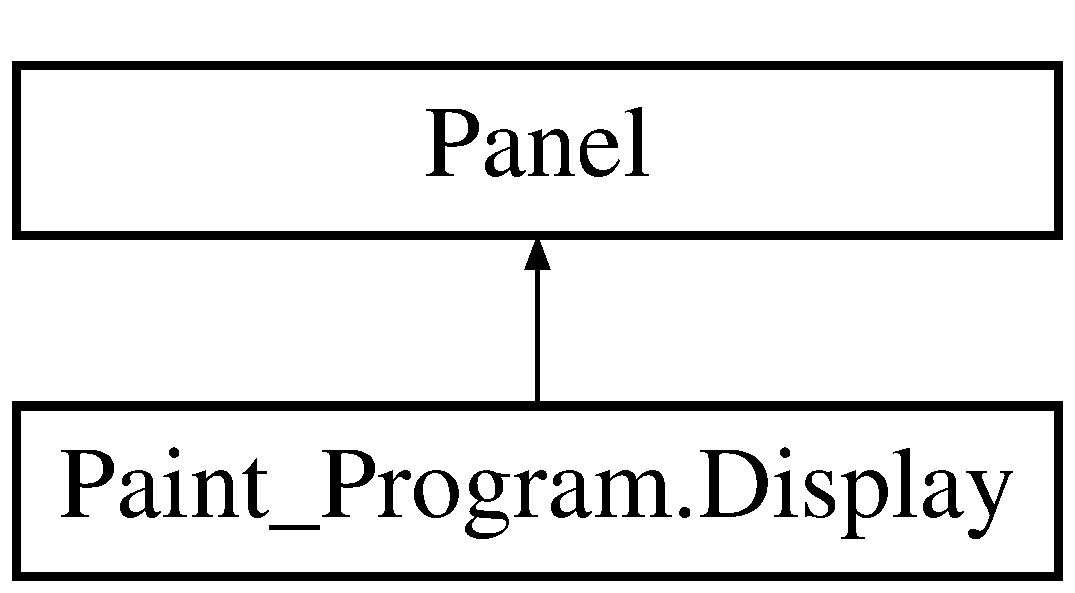
\includegraphics[height=2.000000cm]{class_paint___program_1_1_display}
\end{center}
\end{figure}
\subsection*{Public Member Functions}
\begin{DoxyCompactItemize}
\item 
\mbox{\hyperlink{class_paint___program_1_1_display_ad3ceea08b77033c2ce4ecef813145133}{Display}} ()
\end{DoxyCompactItemize}


\subsection{Constructor \& Destructor Documentation}
\mbox{\Hypertarget{class_paint___program_1_1_display_ad3ceea08b77033c2ce4ecef813145133}\label{class_paint___program_1_1_display_ad3ceea08b77033c2ce4ecef813145133}} 
\index{Paint\+\_\+\+Program\+::\+Display@{Paint\+\_\+\+Program\+::\+Display}!Display@{Display}}
\index{Display@{Display}!Paint\+\_\+\+Program\+::\+Display@{Paint\+\_\+\+Program\+::\+Display}}
\subsubsection{\texorpdfstring{Display()}{Display()}}
{\footnotesize\ttfamily Paint\+\_\+\+Program.\+Display.\+Display (\begin{DoxyParamCaption}{ }\end{DoxyParamCaption})\hspace{0.3cm}{\ttfamily [inline]}}



The documentation for this class was generated from the following file\+:\begin{DoxyCompactItemize}
\item 
Paint Program/\mbox{\hyperlink{_display_8cs}{Display.\+cs}}\end{DoxyCompactItemize}

\hypertarget{class_paint___program_1_1_eraser_tool}{}\section{Paint\+\_\+\+Program.\+Eraser\+Tool Class Reference}
\label{class_paint___program_1_1_eraser_tool}\index{Paint\+\_\+\+Program.\+Eraser\+Tool@{Paint\+\_\+\+Program.\+Eraser\+Tool}}
Inheritance diagram for Paint\+\_\+\+Program.\+Eraser\+Tool\+:\begin{figure}[H]
\begin{center}
\leavevmode
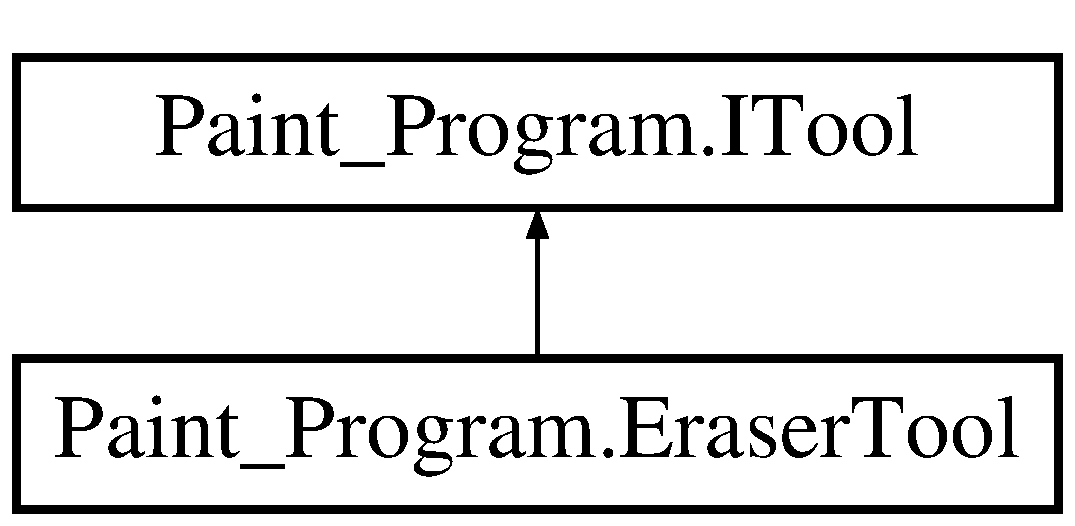
\includegraphics[height=2.000000cm]{class_paint___program_1_1_eraser_tool}
\end{center}
\end{figure}
\subsection*{Public Member Functions}
\begin{DoxyCompactItemize}
\item 
Bitmap \mbox{\hyperlink{class_paint___program_1_1_eraser_tool_ab06fce2e3aefa1a4ce27e861f8036923}{get\+Canvas}} ()
\item 
string \mbox{\hyperlink{class_paint___program_1_1_eraser_tool_a5a1cb5d84a01983064c68a8dc6023ae6}{Get\+Tool\+Icon\+Path}} ()
\item 
void \mbox{\hyperlink{class_paint___program_1_1_eraser_tool_ac19c1e6bfa1b51a384f1f9b1eaa0b2ea}{Init}} ()
\item 
bool \mbox{\hyperlink{class_paint___program_1_1_eraser_tool_a4093d09a604ab0f535497b64447a0013}{is\+Initalized}} ()
\item 
void \mbox{\hyperlink{class_paint___program_1_1_eraser_tool_a4af3cc5379de2a2aec2a5d622801ca86}{On\+Mouse\+Down}} (object sender, Mouse\+Event\+Args e)
\item 
void \mbox{\hyperlink{class_paint___program_1_1_eraser_tool_a1a4e26847ca43fc583017ea76396c19c}{On\+Mouse\+Move}} (object sender, Mouse\+Event\+Args e)
\item 
void \mbox{\hyperlink{class_paint___program_1_1_eraser_tool_aac92273a8f10a9f9cee6e03b1337f1c5}{On\+Mouse\+Up}} (object sender, Mouse\+Event\+Args e)
\item 
Bitmap \mbox{\hyperlink{class_paint___program_1_1_eraser_tool_a2ba0d80771829d2410b5d9a26a6896b2}{Get\+Tool\+Layer}} ()
\item 
bool \mbox{\hyperlink{class_paint___program_1_1_eraser_tool_a2cc4463cfa0525b3687bb227204eaa05}{Requires\+Layer\+Data}} ()
\item 
void \mbox{\hyperlink{class_paint___program_1_1_eraser_tool_ae7daaebe9133c249978d52183a026699}{Set\+Layer\+Data}} (Bitmap bit)
\item 
string \mbox{\hyperlink{class_paint___program_1_1_eraser_tool_ae2c24c146b6269c7eae8b5c196298f5c}{Get\+Tool\+Tip}} ()
\item 
void \mbox{\hyperlink{class_paint___program_1_1_eraser_tool_a0776bb064faa9462f0f224f461a56f31}{Update\+Interface\+Layer}} ()
\end{DoxyCompactItemize}
\subsection*{Private Attributes}
\begin{DoxyCompactItemize}
\item 
Graphics \mbox{\hyperlink{class_paint___program_1_1_eraser_tool_aa794270854644c4048ec6c5c9b736a5a}{graphics}}
\item 
int \mbox{\hyperlink{class_paint___program_1_1_eraser_tool_a1f5259755f77615d916ab2ae24693140}{width}}
\item 
int \mbox{\hyperlink{class_paint___program_1_1_eraser_tool_a0497307d3c637fb660f3c0eff78492dd}{height}}
\item 
bool \mbox{\hyperlink{class_paint___program_1_1_eraser_tool_aa9a395b0a38588a13f4da3051385d681}{b\+Mouse\+Down}}
\item 
bool \mbox{\hyperlink{class_paint___program_1_1_eraser_tool_a35b968ab72538ac17fa1e80514995f32}{b\+Init}}
\item 
Pen \mbox{\hyperlink{class_paint___program_1_1_eraser_tool_a44e140b7e6cba937f70e9a6323e0e6fb}{eraser}}
\item 
Point \mbox{\hyperlink{class_paint___program_1_1_eraser_tool_a269895ea6587d5910d6d5024880fbfd5}{p\+Old}}
\item 
Point \mbox{\hyperlink{class_paint___program_1_1_eraser_tool_ac9df8dc4a5d2881363c0fd652d4b525d}{p\+New}}
\end{DoxyCompactItemize}


\subsection{Member Function Documentation}
\mbox{\Hypertarget{class_paint___program_1_1_eraser_tool_ab06fce2e3aefa1a4ce27e861f8036923}\label{class_paint___program_1_1_eraser_tool_ab06fce2e3aefa1a4ce27e861f8036923}} 
\index{Paint\+\_\+\+Program\+::\+Eraser\+Tool@{Paint\+\_\+\+Program\+::\+Eraser\+Tool}!get\+Canvas@{get\+Canvas}}
\index{get\+Canvas@{get\+Canvas}!Paint\+\_\+\+Program\+::\+Eraser\+Tool@{Paint\+\_\+\+Program\+::\+Eraser\+Tool}}
\subsubsection{\texorpdfstring{get\+Canvas()}{getCanvas()}}
{\footnotesize\ttfamily Bitmap Paint\+\_\+\+Program.\+Eraser\+Tool.\+get\+Canvas (\begin{DoxyParamCaption}{ }\end{DoxyParamCaption})\hspace{0.3cm}{\ttfamily [inline]}}

\mbox{\Hypertarget{class_paint___program_1_1_eraser_tool_a5a1cb5d84a01983064c68a8dc6023ae6}\label{class_paint___program_1_1_eraser_tool_a5a1cb5d84a01983064c68a8dc6023ae6}} 
\index{Paint\+\_\+\+Program\+::\+Eraser\+Tool@{Paint\+\_\+\+Program\+::\+Eraser\+Tool}!Get\+Tool\+Icon\+Path@{Get\+Tool\+Icon\+Path}}
\index{Get\+Tool\+Icon\+Path@{Get\+Tool\+Icon\+Path}!Paint\+\_\+\+Program\+::\+Eraser\+Tool@{Paint\+\_\+\+Program\+::\+Eraser\+Tool}}
\subsubsection{\texorpdfstring{Get\+Tool\+Icon\+Path()}{GetToolIconPath()}}
{\footnotesize\ttfamily string Paint\+\_\+\+Program.\+Eraser\+Tool.\+Get\+Tool\+Icon\+Path (\begin{DoxyParamCaption}{ }\end{DoxyParamCaption})\hspace{0.3cm}{\ttfamily [inline]}}



Implements \mbox{\hyperlink{interface_paint___program_1_1_i_tool_aa057d2f99c59d7bec0215dcad2da1b72}{Paint\+\_\+\+Program.\+I\+Tool}}.

\mbox{\Hypertarget{class_paint___program_1_1_eraser_tool_a2ba0d80771829d2410b5d9a26a6896b2}\label{class_paint___program_1_1_eraser_tool_a2ba0d80771829d2410b5d9a26a6896b2}} 
\index{Paint\+\_\+\+Program\+::\+Eraser\+Tool@{Paint\+\_\+\+Program\+::\+Eraser\+Tool}!Get\+Tool\+Layer@{Get\+Tool\+Layer}}
\index{Get\+Tool\+Layer@{Get\+Tool\+Layer}!Paint\+\_\+\+Program\+::\+Eraser\+Tool@{Paint\+\_\+\+Program\+::\+Eraser\+Tool}}
\subsubsection{\texorpdfstring{Get\+Tool\+Layer()}{GetToolLayer()}}
{\footnotesize\ttfamily Bitmap Paint\+\_\+\+Program.\+Eraser\+Tool.\+Get\+Tool\+Layer (\begin{DoxyParamCaption}{ }\end{DoxyParamCaption})\hspace{0.3cm}{\ttfamily [inline]}}



Implements \mbox{\hyperlink{interface_paint___program_1_1_i_tool_a9b057905515f42a988c166a6a40318e0}{Paint\+\_\+\+Program.\+I\+Tool}}.

\mbox{\Hypertarget{class_paint___program_1_1_eraser_tool_ae2c24c146b6269c7eae8b5c196298f5c}\label{class_paint___program_1_1_eraser_tool_ae2c24c146b6269c7eae8b5c196298f5c}} 
\index{Paint\+\_\+\+Program\+::\+Eraser\+Tool@{Paint\+\_\+\+Program\+::\+Eraser\+Tool}!Get\+Tool\+Tip@{Get\+Tool\+Tip}}
\index{Get\+Tool\+Tip@{Get\+Tool\+Tip}!Paint\+\_\+\+Program\+::\+Eraser\+Tool@{Paint\+\_\+\+Program\+::\+Eraser\+Tool}}
\subsubsection{\texorpdfstring{Get\+Tool\+Tip()}{GetToolTip()}}
{\footnotesize\ttfamily string Paint\+\_\+\+Program.\+Eraser\+Tool.\+Get\+Tool\+Tip (\begin{DoxyParamCaption}{ }\end{DoxyParamCaption})\hspace{0.3cm}{\ttfamily [inline]}}



Implements \mbox{\hyperlink{interface_paint___program_1_1_i_tool_ac11f1591587144b6e74f5767bbf1df56}{Paint\+\_\+\+Program.\+I\+Tool}}.

\mbox{\Hypertarget{class_paint___program_1_1_eraser_tool_ac19c1e6bfa1b51a384f1f9b1eaa0b2ea}\label{class_paint___program_1_1_eraser_tool_ac19c1e6bfa1b51a384f1f9b1eaa0b2ea}} 
\index{Paint\+\_\+\+Program\+::\+Eraser\+Tool@{Paint\+\_\+\+Program\+::\+Eraser\+Tool}!Init@{Init}}
\index{Init@{Init}!Paint\+\_\+\+Program\+::\+Eraser\+Tool@{Paint\+\_\+\+Program\+::\+Eraser\+Tool}}
\subsubsection{\texorpdfstring{Init()}{Init()}}
{\footnotesize\ttfamily void Paint\+\_\+\+Program.\+Eraser\+Tool.\+Init (\begin{DoxyParamCaption}{ }\end{DoxyParamCaption})\hspace{0.3cm}{\ttfamily [inline]}}



Implements \mbox{\hyperlink{interface_paint___program_1_1_i_tool_af823123a30fbda34e24e907243241046}{Paint\+\_\+\+Program.\+I\+Tool}}.

\mbox{\Hypertarget{class_paint___program_1_1_eraser_tool_a4093d09a604ab0f535497b64447a0013}\label{class_paint___program_1_1_eraser_tool_a4093d09a604ab0f535497b64447a0013}} 
\index{Paint\+\_\+\+Program\+::\+Eraser\+Tool@{Paint\+\_\+\+Program\+::\+Eraser\+Tool}!is\+Initalized@{is\+Initalized}}
\index{is\+Initalized@{is\+Initalized}!Paint\+\_\+\+Program\+::\+Eraser\+Tool@{Paint\+\_\+\+Program\+::\+Eraser\+Tool}}
\subsubsection{\texorpdfstring{is\+Initalized()}{isInitalized()}}
{\footnotesize\ttfamily bool Paint\+\_\+\+Program.\+Eraser\+Tool.\+is\+Initalized (\begin{DoxyParamCaption}{ }\end{DoxyParamCaption})\hspace{0.3cm}{\ttfamily [inline]}}



Implements \mbox{\hyperlink{interface_paint___program_1_1_i_tool_a951b844bcbf47a6c306104fa86be7a5d}{Paint\+\_\+\+Program.\+I\+Tool}}.

\mbox{\Hypertarget{class_paint___program_1_1_eraser_tool_a4af3cc5379de2a2aec2a5d622801ca86}\label{class_paint___program_1_1_eraser_tool_a4af3cc5379de2a2aec2a5d622801ca86}} 
\index{Paint\+\_\+\+Program\+::\+Eraser\+Tool@{Paint\+\_\+\+Program\+::\+Eraser\+Tool}!On\+Mouse\+Down@{On\+Mouse\+Down}}
\index{On\+Mouse\+Down@{On\+Mouse\+Down}!Paint\+\_\+\+Program\+::\+Eraser\+Tool@{Paint\+\_\+\+Program\+::\+Eraser\+Tool}}
\subsubsection{\texorpdfstring{On\+Mouse\+Down()}{OnMouseDown()}}
{\footnotesize\ttfamily void Paint\+\_\+\+Program.\+Eraser\+Tool.\+On\+Mouse\+Down (\begin{DoxyParamCaption}\item[{object}]{sender,  }\item[{Mouse\+Event\+Args}]{e }\end{DoxyParamCaption})\hspace{0.3cm}{\ttfamily [inline]}}



Implements \mbox{\hyperlink{interface_paint___program_1_1_i_tool_a73d8797f4f2b1e0d8efe8aadcd44e840}{Paint\+\_\+\+Program.\+I\+Tool}}.

\mbox{\Hypertarget{class_paint___program_1_1_eraser_tool_a1a4e26847ca43fc583017ea76396c19c}\label{class_paint___program_1_1_eraser_tool_a1a4e26847ca43fc583017ea76396c19c}} 
\index{Paint\+\_\+\+Program\+::\+Eraser\+Tool@{Paint\+\_\+\+Program\+::\+Eraser\+Tool}!On\+Mouse\+Move@{On\+Mouse\+Move}}
\index{On\+Mouse\+Move@{On\+Mouse\+Move}!Paint\+\_\+\+Program\+::\+Eraser\+Tool@{Paint\+\_\+\+Program\+::\+Eraser\+Tool}}
\subsubsection{\texorpdfstring{On\+Mouse\+Move()}{OnMouseMove()}}
{\footnotesize\ttfamily void Paint\+\_\+\+Program.\+Eraser\+Tool.\+On\+Mouse\+Move (\begin{DoxyParamCaption}\item[{object}]{sender,  }\item[{Mouse\+Event\+Args}]{e }\end{DoxyParamCaption})\hspace{0.3cm}{\ttfamily [inline]}}



Implements \mbox{\hyperlink{interface_paint___program_1_1_i_tool_a6a1cbe840b5cfc8a9b9463cc21590845}{Paint\+\_\+\+Program.\+I\+Tool}}.

\mbox{\Hypertarget{class_paint___program_1_1_eraser_tool_aac92273a8f10a9f9cee6e03b1337f1c5}\label{class_paint___program_1_1_eraser_tool_aac92273a8f10a9f9cee6e03b1337f1c5}} 
\index{Paint\+\_\+\+Program\+::\+Eraser\+Tool@{Paint\+\_\+\+Program\+::\+Eraser\+Tool}!On\+Mouse\+Up@{On\+Mouse\+Up}}
\index{On\+Mouse\+Up@{On\+Mouse\+Up}!Paint\+\_\+\+Program\+::\+Eraser\+Tool@{Paint\+\_\+\+Program\+::\+Eraser\+Tool}}
\subsubsection{\texorpdfstring{On\+Mouse\+Up()}{OnMouseUp()}}
{\footnotesize\ttfamily void Paint\+\_\+\+Program.\+Eraser\+Tool.\+On\+Mouse\+Up (\begin{DoxyParamCaption}\item[{object}]{sender,  }\item[{Mouse\+Event\+Args}]{e }\end{DoxyParamCaption})\hspace{0.3cm}{\ttfamily [inline]}}



Implements \mbox{\hyperlink{interface_paint___program_1_1_i_tool_a47984c2879213022f1684c07f7bba73e}{Paint\+\_\+\+Program.\+I\+Tool}}.

\mbox{\Hypertarget{class_paint___program_1_1_eraser_tool_a2cc4463cfa0525b3687bb227204eaa05}\label{class_paint___program_1_1_eraser_tool_a2cc4463cfa0525b3687bb227204eaa05}} 
\index{Paint\+\_\+\+Program\+::\+Eraser\+Tool@{Paint\+\_\+\+Program\+::\+Eraser\+Tool}!Requires\+Layer\+Data@{Requires\+Layer\+Data}}
\index{Requires\+Layer\+Data@{Requires\+Layer\+Data}!Paint\+\_\+\+Program\+::\+Eraser\+Tool@{Paint\+\_\+\+Program\+::\+Eraser\+Tool}}
\subsubsection{\texorpdfstring{Requires\+Layer\+Data()}{RequiresLayerData()}}
{\footnotesize\ttfamily bool Paint\+\_\+\+Program.\+Eraser\+Tool.\+Requires\+Layer\+Data (\begin{DoxyParamCaption}{ }\end{DoxyParamCaption})\hspace{0.3cm}{\ttfamily [inline]}}



Implements \mbox{\hyperlink{interface_paint___program_1_1_i_tool_a6d45b6c48da8130ae41db3a66cdaef9a}{Paint\+\_\+\+Program.\+I\+Tool}}.

\mbox{\Hypertarget{class_paint___program_1_1_eraser_tool_ae7daaebe9133c249978d52183a026699}\label{class_paint___program_1_1_eraser_tool_ae7daaebe9133c249978d52183a026699}} 
\index{Paint\+\_\+\+Program\+::\+Eraser\+Tool@{Paint\+\_\+\+Program\+::\+Eraser\+Tool}!Set\+Layer\+Data@{Set\+Layer\+Data}}
\index{Set\+Layer\+Data@{Set\+Layer\+Data}!Paint\+\_\+\+Program\+::\+Eraser\+Tool@{Paint\+\_\+\+Program\+::\+Eraser\+Tool}}
\subsubsection{\texorpdfstring{Set\+Layer\+Data()}{SetLayerData()}}
{\footnotesize\ttfamily void Paint\+\_\+\+Program.\+Eraser\+Tool.\+Set\+Layer\+Data (\begin{DoxyParamCaption}\item[{Bitmap}]{bit }\end{DoxyParamCaption})\hspace{0.3cm}{\ttfamily [inline]}}



Implements \mbox{\hyperlink{interface_paint___program_1_1_i_tool_a2d3e63715dfe04075d27dacf367d1633}{Paint\+\_\+\+Program.\+I\+Tool}}.

\mbox{\Hypertarget{class_paint___program_1_1_eraser_tool_a0776bb064faa9462f0f224f461a56f31}\label{class_paint___program_1_1_eraser_tool_a0776bb064faa9462f0f224f461a56f31}} 
\index{Paint\+\_\+\+Program\+::\+Eraser\+Tool@{Paint\+\_\+\+Program\+::\+Eraser\+Tool}!Update\+Interface\+Layer@{Update\+Interface\+Layer}}
\index{Update\+Interface\+Layer@{Update\+Interface\+Layer}!Paint\+\_\+\+Program\+::\+Eraser\+Tool@{Paint\+\_\+\+Program\+::\+Eraser\+Tool}}
\subsubsection{\texorpdfstring{Update\+Interface\+Layer()}{UpdateInterfaceLayer()}}
{\footnotesize\ttfamily void Paint\+\_\+\+Program.\+Eraser\+Tool.\+Update\+Interface\+Layer (\begin{DoxyParamCaption}{ }\end{DoxyParamCaption})\hspace{0.3cm}{\ttfamily [inline]}}



Implements \mbox{\hyperlink{interface_paint___program_1_1_i_tool_a36db75d29e88dfd739f658633c40e955}{Paint\+\_\+\+Program.\+I\+Tool}}.



\subsection{Member Data Documentation}
\mbox{\Hypertarget{class_paint___program_1_1_eraser_tool_a35b968ab72538ac17fa1e80514995f32}\label{class_paint___program_1_1_eraser_tool_a35b968ab72538ac17fa1e80514995f32}} 
\index{Paint\+\_\+\+Program\+::\+Eraser\+Tool@{Paint\+\_\+\+Program\+::\+Eraser\+Tool}!b\+Init@{b\+Init}}
\index{b\+Init@{b\+Init}!Paint\+\_\+\+Program\+::\+Eraser\+Tool@{Paint\+\_\+\+Program\+::\+Eraser\+Tool}}
\subsubsection{\texorpdfstring{b\+Init}{bInit}}
{\footnotesize\ttfamily bool Paint\+\_\+\+Program.\+Eraser\+Tool.\+b\+Init\hspace{0.3cm}{\ttfamily [private]}}

\mbox{\Hypertarget{class_paint___program_1_1_eraser_tool_aa9a395b0a38588a13f4da3051385d681}\label{class_paint___program_1_1_eraser_tool_aa9a395b0a38588a13f4da3051385d681}} 
\index{Paint\+\_\+\+Program\+::\+Eraser\+Tool@{Paint\+\_\+\+Program\+::\+Eraser\+Tool}!b\+Mouse\+Down@{b\+Mouse\+Down}}
\index{b\+Mouse\+Down@{b\+Mouse\+Down}!Paint\+\_\+\+Program\+::\+Eraser\+Tool@{Paint\+\_\+\+Program\+::\+Eraser\+Tool}}
\subsubsection{\texorpdfstring{b\+Mouse\+Down}{bMouseDown}}
{\footnotesize\ttfamily bool Paint\+\_\+\+Program.\+Eraser\+Tool.\+b\+Mouse\+Down\hspace{0.3cm}{\ttfamily [private]}}

\mbox{\Hypertarget{class_paint___program_1_1_eraser_tool_a44e140b7e6cba937f70e9a6323e0e6fb}\label{class_paint___program_1_1_eraser_tool_a44e140b7e6cba937f70e9a6323e0e6fb}} 
\index{Paint\+\_\+\+Program\+::\+Eraser\+Tool@{Paint\+\_\+\+Program\+::\+Eraser\+Tool}!eraser@{eraser}}
\index{eraser@{eraser}!Paint\+\_\+\+Program\+::\+Eraser\+Tool@{Paint\+\_\+\+Program\+::\+Eraser\+Tool}}
\subsubsection{\texorpdfstring{eraser}{eraser}}
{\footnotesize\ttfamily Pen Paint\+\_\+\+Program.\+Eraser\+Tool.\+eraser\hspace{0.3cm}{\ttfamily [private]}}

\mbox{\Hypertarget{class_paint___program_1_1_eraser_tool_aa794270854644c4048ec6c5c9b736a5a}\label{class_paint___program_1_1_eraser_tool_aa794270854644c4048ec6c5c9b736a5a}} 
\index{Paint\+\_\+\+Program\+::\+Eraser\+Tool@{Paint\+\_\+\+Program\+::\+Eraser\+Tool}!graphics@{graphics}}
\index{graphics@{graphics}!Paint\+\_\+\+Program\+::\+Eraser\+Tool@{Paint\+\_\+\+Program\+::\+Eraser\+Tool}}
\subsubsection{\texorpdfstring{graphics}{graphics}}
{\footnotesize\ttfamily Graphics Paint\+\_\+\+Program.\+Eraser\+Tool.\+graphics\hspace{0.3cm}{\ttfamily [private]}}

\mbox{\Hypertarget{class_paint___program_1_1_eraser_tool_a0497307d3c637fb660f3c0eff78492dd}\label{class_paint___program_1_1_eraser_tool_a0497307d3c637fb660f3c0eff78492dd}} 
\index{Paint\+\_\+\+Program\+::\+Eraser\+Tool@{Paint\+\_\+\+Program\+::\+Eraser\+Tool}!height@{height}}
\index{height@{height}!Paint\+\_\+\+Program\+::\+Eraser\+Tool@{Paint\+\_\+\+Program\+::\+Eraser\+Tool}}
\subsubsection{\texorpdfstring{height}{height}}
{\footnotesize\ttfamily int Paint\+\_\+\+Program.\+Eraser\+Tool.\+height\hspace{0.3cm}{\ttfamily [private]}}

\mbox{\Hypertarget{class_paint___program_1_1_eraser_tool_ac9df8dc4a5d2881363c0fd652d4b525d}\label{class_paint___program_1_1_eraser_tool_ac9df8dc4a5d2881363c0fd652d4b525d}} 
\index{Paint\+\_\+\+Program\+::\+Eraser\+Tool@{Paint\+\_\+\+Program\+::\+Eraser\+Tool}!p\+New@{p\+New}}
\index{p\+New@{p\+New}!Paint\+\_\+\+Program\+::\+Eraser\+Tool@{Paint\+\_\+\+Program\+::\+Eraser\+Tool}}
\subsubsection{\texorpdfstring{p\+New}{pNew}}
{\footnotesize\ttfamily Point Paint\+\_\+\+Program.\+Eraser\+Tool.\+p\+New\hspace{0.3cm}{\ttfamily [private]}}

\mbox{\Hypertarget{class_paint___program_1_1_eraser_tool_a269895ea6587d5910d6d5024880fbfd5}\label{class_paint___program_1_1_eraser_tool_a269895ea6587d5910d6d5024880fbfd5}} 
\index{Paint\+\_\+\+Program\+::\+Eraser\+Tool@{Paint\+\_\+\+Program\+::\+Eraser\+Tool}!p\+Old@{p\+Old}}
\index{p\+Old@{p\+Old}!Paint\+\_\+\+Program\+::\+Eraser\+Tool@{Paint\+\_\+\+Program\+::\+Eraser\+Tool}}
\subsubsection{\texorpdfstring{p\+Old}{pOld}}
{\footnotesize\ttfamily Point Paint\+\_\+\+Program.\+Eraser\+Tool.\+p\+Old\hspace{0.3cm}{\ttfamily [private]}}

\mbox{\Hypertarget{class_paint___program_1_1_eraser_tool_a1f5259755f77615d916ab2ae24693140}\label{class_paint___program_1_1_eraser_tool_a1f5259755f77615d916ab2ae24693140}} 
\index{Paint\+\_\+\+Program\+::\+Eraser\+Tool@{Paint\+\_\+\+Program\+::\+Eraser\+Tool}!width@{width}}
\index{width@{width}!Paint\+\_\+\+Program\+::\+Eraser\+Tool@{Paint\+\_\+\+Program\+::\+Eraser\+Tool}}
\subsubsection{\texorpdfstring{width}{width}}
{\footnotesize\ttfamily int Paint\+\_\+\+Program.\+Eraser\+Tool.\+width\hspace{0.3cm}{\ttfamily [private]}}



The documentation for this class was generated from the following file\+:\begin{DoxyCompactItemize}
\item 
Paint Program/\mbox{\hyperlink{_eraser_tool_8cs}{Eraser\+Tool.\+cs}}\end{DoxyCompactItemize}

\hypertarget{class_paint___program_1_1_file_save}{}\section{Paint\+\_\+\+Program.\+File\+Save Class Reference}
\label{class_paint___program_1_1_file_save}\index{Paint\+\_\+\+Program.\+File\+Save@{Paint\+\_\+\+Program.\+File\+Save}}
\subsection*{Public Member Functions}
\begin{DoxyCompactItemize}
\item 
\mbox{\hyperlink{class_paint___program_1_1_file_save_a8f1d802c4dccb8b60bd56c723348d8e8}{File\+Save}} ()
\end{DoxyCompactItemize}
\subsection*{Private Member Functions}
\begin{DoxyCompactItemize}
\item 
void \mbox{\hyperlink{class_paint___program_1_1_file_save_ad180b279d4ba8813fa777acd386665ac}{do\+Save}} (Bitmap bm, Save\+File\+Dialog sfd, object sender, Do\+Work\+Event\+Args args)
\item 
void \mbox{\hyperlink{class_paint___program_1_1_file_save_a2ca61f0383c371f649c95825d40795f6}{save\+G\+I\+F\+Animation}} (System.\+I\+O.\+File\+Stream fs)
\end{DoxyCompactItemize}


\subsection{Constructor \& Destructor Documentation}
\mbox{\Hypertarget{class_paint___program_1_1_file_save_a8f1d802c4dccb8b60bd56c723348d8e8}\label{class_paint___program_1_1_file_save_a8f1d802c4dccb8b60bd56c723348d8e8}} 
\index{Paint\+\_\+\+Program\+::\+File\+Save@{Paint\+\_\+\+Program\+::\+File\+Save}!File\+Save@{File\+Save}}
\index{File\+Save@{File\+Save}!Paint\+\_\+\+Program\+::\+File\+Save@{Paint\+\_\+\+Program\+::\+File\+Save}}
\subsubsection{\texorpdfstring{File\+Save()}{FileSave()}}
{\footnotesize\ttfamily Paint\+\_\+\+Program.\+File\+Save.\+File\+Save (\begin{DoxyParamCaption}{ }\end{DoxyParamCaption})\hspace{0.3cm}{\ttfamily [inline]}}



\subsection{Member Function Documentation}
\mbox{\Hypertarget{class_paint___program_1_1_file_save_ad180b279d4ba8813fa777acd386665ac}\label{class_paint___program_1_1_file_save_ad180b279d4ba8813fa777acd386665ac}} 
\index{Paint\+\_\+\+Program\+::\+File\+Save@{Paint\+\_\+\+Program\+::\+File\+Save}!do\+Save@{do\+Save}}
\index{do\+Save@{do\+Save}!Paint\+\_\+\+Program\+::\+File\+Save@{Paint\+\_\+\+Program\+::\+File\+Save}}
\subsubsection{\texorpdfstring{do\+Save()}{doSave()}}
{\footnotesize\ttfamily void Paint\+\_\+\+Program.\+File\+Save.\+do\+Save (\begin{DoxyParamCaption}\item[{Bitmap}]{bm,  }\item[{Save\+File\+Dialog}]{sfd,  }\item[{object}]{sender,  }\item[{Do\+Work\+Event\+Args}]{args }\end{DoxyParamCaption})\hspace{0.3cm}{\ttfamily [inline]}, {\ttfamily [private]}}

\mbox{\Hypertarget{class_paint___program_1_1_file_save_a2ca61f0383c371f649c95825d40795f6}\label{class_paint___program_1_1_file_save_a2ca61f0383c371f649c95825d40795f6}} 
\index{Paint\+\_\+\+Program\+::\+File\+Save@{Paint\+\_\+\+Program\+::\+File\+Save}!save\+G\+I\+F\+Animation@{save\+G\+I\+F\+Animation}}
\index{save\+G\+I\+F\+Animation@{save\+G\+I\+F\+Animation}!Paint\+\_\+\+Program\+::\+File\+Save@{Paint\+\_\+\+Program\+::\+File\+Save}}
\subsubsection{\texorpdfstring{save\+G\+I\+F\+Animation()}{saveGIFAnimation()}}
{\footnotesize\ttfamily void Paint\+\_\+\+Program.\+File\+Save.\+save\+G\+I\+F\+Animation (\begin{DoxyParamCaption}\item[{System.\+I\+O.\+File\+Stream}]{fs }\end{DoxyParamCaption})\hspace{0.3cm}{\ttfamily [inline]}, {\ttfamily [private]}}



The documentation for this class was generated from the following file\+:\begin{DoxyCompactItemize}
\item 
Paint Program/\mbox{\hyperlink{_file_save_8cs}{File\+Save.\+cs}}\end{DoxyCompactItemize}

\hypertarget{class_wintab_d_n_1_1_f_i_x32}{}\section{Wintab\+D\+N.\+F\+I\+X32 Class Reference}
\label{class_wintab_d_n_1_1_f_i_x32}\index{Wintab\+D\+N.\+F\+I\+X32@{Wintab\+D\+N.\+F\+I\+X32}}


Managed implementation of Wintab \mbox{\hyperlink{class_wintab_d_n_1_1_f_i_x32}{F\+I\+X32}} typedef. Used for a fixed-\/point arithmetic value.  




\subsection{Detailed Description}
Managed implementation of Wintab \mbox{\hyperlink{class_wintab_d_n_1_1_f_i_x32}{F\+I\+X32}} typedef. Used for a fixed-\/point arithmetic value. 



The documentation for this class was generated from the following file\+:\begin{DoxyCompactItemize}
\item 
Wintab\+D\+N/\mbox{\hyperlink{_c_wintab_funcs_8cs}{C\+Wintab\+Funcs.\+cs}}\end{DoxyCompactItemize}

\hypertarget{class_paint___program_1_1_form1}{}\section{Paint\+\_\+\+Program.\+Form1 Class Reference}
\label{class_paint___program_1_1_form1}\index{Paint\+\_\+\+Program.\+Form1@{Paint\+\_\+\+Program.\+Form1}}
Inheritance diagram for Paint\+\_\+\+Program.\+Form1\+:\begin{figure}[H]
\begin{center}
\leavevmode
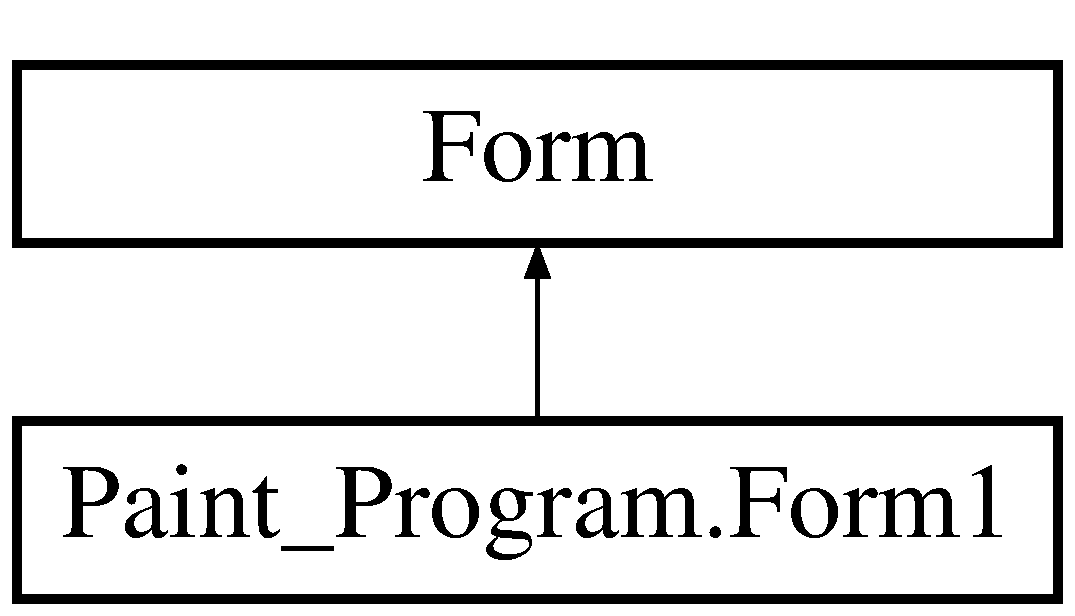
\includegraphics[height=2.000000cm]{class_paint___program_1_1_form1}
\end{center}
\end{figure}
\subsection*{Public Member Functions}
\begin{DoxyCompactItemize}
\item 
\mbox{\hyperlink{class_paint___program_1_1_form1_aefb0d3ee7baac9f44e9d742615ec526d}{Form1}} ()
\item 
void \mbox{\hyperlink{class_paint___program_1_1_form1_a3d5993c6aaba845e13b8b5d76e38f447}{Update\+Views}} ()
\end{DoxyCompactItemize}
\subsection*{Protected Member Functions}
\begin{DoxyCompactItemize}
\item 
override void \mbox{\hyperlink{class_paint___program_1_1_form1_a0bd4c16e36005c28132ae0785f626e90}{Dispose}} (bool disposing)
\begin{DoxyCompactList}\small\item\em Clean up any resources being used. \end{DoxyCompactList}\end{DoxyCompactItemize}
\subsection*{Private Member Functions}
\begin{DoxyCompactItemize}
\item 
void \mbox{\hyperlink{class_paint___program_1_1_form1_a616e4f7ed06b9d03f9794c6150c55bec}{Populate\+Languages}} ()
\item 
void \mbox{\hyperlink{class_paint___program_1_1_form1_a14fd317ce19e4a4c5cd44aba2ea750a1}{Update\+Text}} ()
\item 
void \mbox{\hyperlink{class_paint___program_1_1_form1_ade0d4d5a5b74af8a5ee99912745632d7}{Tsmi\+File\+\_\+\+New\+\_\+\+Click}} (object sender, Event\+Args e)
\item 
void \mbox{\hyperlink{class_paint___program_1_1_form1_a39a6d9fbd5f250daa6fdbdc3d427c743}{Clear\+Controls}} ()
\item 
void \mbox{\hyperlink{class_paint___program_1_1_form1_ae2b2f92fe493ccef4b1c943ecc98f693}{Make\+New\+Project}} (int w, int h)
\item 
void \mbox{\hyperlink{class_paint___program_1_1_form1_a2aa0c38b6361f4992c9837e7819e01ee}{Make\+New\+Project}} ()
\item 
void \mbox{\hyperlink{class_paint___program_1_1_form1_ad6ed55aa3e56805f2657b831f49f6331}{Tsmi\+File\+\_\+\+Save\+\_\+\+Click}} (object sender, Event\+Args e)
\item 
void \mbox{\hyperlink{class_paint___program_1_1_form1_af074be280a47db857d9b7d649fb23932}{Tsmi\+File\+\_\+\+Import\+\_\+\+Click}} (object sender, Event\+Args e)
\item 
void \mbox{\hyperlink{class_paint___program_1_1_form1_a12af75ac6e998a5d7091c51368e0ab1c}{Tsmi\+File\+\_\+\+Export\+\_\+\+Click}} (object sender, Event\+Args e)
\item 
void \mbox{\hyperlink{class_paint___program_1_1_form1_a3fd2977a63399c5cf772ba43a085291d}{Tsmi\+Edit\+\_\+\+Undo\+\_\+\+Click}} (object sender, Event\+Args e)
\item 
void \mbox{\hyperlink{class_paint___program_1_1_form1_aae2330807cd6eaacb82e143b2ffbe668}{Tsmi\+Edit\+\_\+\+Redo\+\_\+\+Click}} (object sender, Event\+Args e)
\item 
void \mbox{\hyperlink{class_paint___program_1_1_form1_a1034728c62e4c62d618133811093749f}{Tsmi\+Edit\+\_\+\+Image\+Size\+\_\+\+Click}} (object sender, Event\+Args e)
\item 
void \mbox{\hyperlink{class_paint___program_1_1_form1_a97c7127920edd9d1039c0b6429d5649c}{Tsmi\+View\+\_\+\+Tablet\+\_\+\+Click}} (object sender, Event\+Args e)
\item 
void \mbox{\hyperlink{class_paint___program_1_1_form1_aa2e74c2cba3ed25148c8233b4cdf9534}{Tsmi\+View\+\_\+\+Show\+Tools\+\_\+\+Click}} (object sender, Event\+Args e)
\item 
void \mbox{\hyperlink{class_paint___program_1_1_form1_ae97d925efefbb28724feae4ac62f3969}{Tsmi\+File\+\_\+\+Load\+\_\+\+Click}} (object sender, Event\+Args e)
\item 
void \mbox{\hyperlink{class_paint___program_1_1_form1_ab504b6a4767e30549d06c4e4816fabae}{Tsmi\+View\+\_\+\+Grid\+Lines\+\_\+5\+\_\+\+Click}} (object sender, Event\+Args e)
\item 
void \mbox{\hyperlink{class_paint___program_1_1_form1_adb0b989f2e72eb718d5a7189484ac4c6}{Tsmi\+View\+\_\+\+Grid\+Lines\+\_\+10\+\_\+\+Click}} (object sender, Event\+Args e)
\item 
void \mbox{\hyperlink{class_paint___program_1_1_form1_ad1220fb8f568478e58db7e778fce5c37}{Tsmi\+View\+\_\+\+Grid\+Lines\+\_\+25\+\_\+\+Click}} (object sender, Event\+Args e)
\item 
void \mbox{\hyperlink{class_paint___program_1_1_form1_a9488136e6f66de4b3e7cdf54659bfe20}{Tsmi\+View\+\_\+\+Grid\+Lines\+\_\+50\+\_\+\+Click}} (object sender, Event\+Args e)
\item 
void \mbox{\hyperlink{class_paint___program_1_1_form1_a777afbe5c0f7d7654f4f4a0962d0feea}{Tsmi\+View\+\_\+\+Grid\+Lines\+\_\+100\+\_\+\+Click}} (object sender, Event\+Args e)
\item 
void \mbox{\hyperlink{class_paint___program_1_1_form1_a833a4da8414e842babafe6a034f2919f}{Tsmi\+View\+\_\+\+Grid\+Lines\+\_\+\+Auto\+\_\+\+Click}} (object sender, Event\+Args e)
\item 
void \mbox{\hyperlink{class_paint___program_1_1_form1_a2531d9adc858d169c9d5ae28f5f37167}{Grid\+Uncheck}} ()
\item 
void \mbox{\hyperlink{class_paint___program_1_1_form1_ae896493468ffcf8b621a014f6a0553a3}{Ts\+New\+\_\+\+Click}} (object sender, Event\+Args e)
\item 
void \mbox{\hyperlink{class_paint___program_1_1_form1_adf420684ede06a8c00802959aa1959e9}{Ts\+Open\+\_\+\+Click}} (object sender, Event\+Args e)
\item 
void \mbox{\hyperlink{class_paint___program_1_1_form1_a4e1485fafb2460d9e028a6fb3c8494e0}{Ts\+Save\+\_\+\+Click}} (object sender, Event\+Args e)
\item 
void \mbox{\hyperlink{class_paint___program_1_1_form1_a4748a20826e99235f5fa467335383da4}{Ts\+Import\+\_\+\+Click}} (object sender, Event\+Args e)
\item 
void \mbox{\hyperlink{class_paint___program_1_1_form1_a029f8130f202c343547662281dd3b579}{Ts\+Export\+\_\+\+Click}} (object sender, Event\+Args e)
\item 
void \mbox{\hyperlink{class_paint___program_1_1_form1_a5a68e92cce596c404c124632a816f1a8}{Set\+Image\+Tool\+Strip\+Menu\+Item\+\_\+\+Click}} (object sender, Event\+Args e)
\item 
void \mbox{\hyperlink{class_paint___program_1_1_form1_aef82c4e95b5665684979ac3a80ab9d1b}{Show\+Watermark\+Tool\+Strip\+Menu\+Item\+\_\+\+Click}} (object sender, Event\+Args e)
\item 
void \mbox{\hyperlink{class_paint___program_1_1_form1_ab63c1cf093277a8090c5320d01ac15a4}{Tsmi\+Preferences\+\_\+\+Watermark\+\_\+\+Single\+Center\+\_\+\+Click}} (object sender, Event\+Args e)
\item 
void \mbox{\hyperlink{class_paint___program_1_1_form1_a865d2bb002b7ee82f9c395577b1b3d0c}{Tsmi\+Preferences\+\_\+\+Watermark\+\_\+\+Single\+Bottom\+\_\+\+Click}} (object sender, Event\+Args e)
\item 
void \mbox{\hyperlink{class_paint___program_1_1_form1_a45bd276e52f9e8bf269c504c8ec618a6}{Tsmi\+Preferences\+\_\+\+Watermark\+\_\+\+Tiled\+\_\+\+Click}} (object sender, Event\+Args e)
\item 
void \mbox{\hyperlink{class_paint___program_1_1_form1_aa5747a15abf1a595a61fea3cad264b64}{Tsmi\+File\+\_\+\+Save\+Google\+Drive\+\_\+\+Click}} (object sender, Event\+Args e)
\item 
void \mbox{\hyperlink{class_paint___program_1_1_form1_aad3ab339698773a2374c8d7010435ed9}{Form1\+\_\+\+Key\+Down}} (object sender, Key\+Event\+Args e)
\begin{DoxyCompactList}\small\item\em Handles key down events and processes keyboard shortcut combinations ~\newline
 \end{DoxyCompactList}\item 
void \mbox{\hyperlink{class_paint___program_1_1_form1_adc345c6a01064caac3ad12472221150c}{Copy\+Selection\+To\+Clipboard}} ()
\item 
Image \mbox{\hyperlink{class_paint___program_1_1_form1_a46dce5128798bdc15d8fade229630ec0}{Get\+Clipboard\+Image}} ()
\item 
void \mbox{\hyperlink{class_paint___program_1_1_form1_a0c2c0648cdef32547fed28e522cf0cbe}{Initialize\+Component}} ()
\begin{DoxyCompactList}\small\item\em Required method for Designer support -\/ do not modify the contents of this method with the code editor. \end{DoxyCompactList}\end{DoxyCompactItemize}
\subsection*{Private Attributes}
\begin{DoxyCompactItemize}
\item 
\mbox{\hyperlink{class_paint___program_1_1_canvas}{Canvas}} \mbox{\hyperlink{class_paint___program_1_1_form1_ae97aba2c6b8ee08da0b3af7bd7943c4a}{c}}
\item 
System.\+Component\+Model.\+I\+Container \mbox{\hyperlink{class_paint___program_1_1_form1_a95d0a7a8fc7be660e77f445b4562cd2f}{components}} = null
\begin{DoxyCompactList}\small\item\em Required designer variable. \end{DoxyCompactList}\item 
System.\+Windows.\+Forms.\+Menu\+Strip \mbox{\hyperlink{class_paint___program_1_1_form1_a2ec5d48907647eb6f3385b7e567d2a20}{ms\+Menu}}
\item 
System.\+Windows.\+Forms.\+Tool\+Strip\+Menu\+Item \mbox{\hyperlink{class_paint___program_1_1_form1_a82f2c6d2129b75a00b4743e4e8bc10f6}{tsmi\+File}}
\item 
System.\+Windows.\+Forms.\+Tool\+Strip\+Menu\+Item \mbox{\hyperlink{class_paint___program_1_1_form1_af4f5842df653b0c2601897af26b651c9}{tsmi\+File\+\_\+\+New}}
\item 
System.\+Windows.\+Forms.\+Timer \mbox{\hyperlink{class_paint___program_1_1_form1_acecdd498b40a257daf3424d49e172a9d}{update\+Timer}}
\item 
System.\+Windows.\+Forms.\+Tool\+Strip\+Menu\+Item \mbox{\hyperlink{class_paint___program_1_1_form1_a9164e5083cda36098e27bb7efcae5789}{tsmi\+File\+\_\+\+Save}}
\item 
System.\+Windows.\+Forms.\+Tool\+Strip\+Menu\+Item \mbox{\hyperlink{class_paint___program_1_1_form1_aa972312f80850f6519a48e363c504835}{tsmi\+File\+\_\+\+Import}}
\item 
System.\+Windows.\+Forms.\+Tool\+Strip\+Menu\+Item \mbox{\hyperlink{class_paint___program_1_1_form1_ad340dfd4c776702545d1261d02b2cb9d}{tsmi\+File\+\_\+\+Export}}
\item 
System.\+Windows.\+Forms.\+Tool\+Strip\+Menu\+Item \mbox{\hyperlink{class_paint___program_1_1_form1_af08d32364512b4ad007a3ea94f61bd8f}{tsmi\+Edit}}
\item 
System.\+Windows.\+Forms.\+Tool\+Strip\+Menu\+Item \mbox{\hyperlink{class_paint___program_1_1_form1_a2343678a0dc95da2347f6f12a2b6aabf}{tsmi\+Edit\+\_\+\+Undo}}
\item 
System.\+Windows.\+Forms.\+Tool\+Strip\+Menu\+Item \mbox{\hyperlink{class_paint___program_1_1_form1_ab8e2071c6763b0d0f4b1e001ea4eca97}{tsmi\+Edit\+\_\+\+Redo}}
\item 
System.\+Windows.\+Forms.\+Tool\+Strip\+Menu\+Item \mbox{\hyperlink{class_paint___program_1_1_form1_ab77fd9bb3a148f2228e9390c335c8350}{tsmi\+Edit\+\_\+\+Resize}}
\item 
System.\+Windows.\+Forms.\+Tool\+Strip\+Menu\+Item \mbox{\hyperlink{class_paint___program_1_1_form1_aa47b36feef8f0c4044d1c915d432101b}{tsmi\+View}}
\item 
System.\+Windows.\+Forms.\+Tool\+Strip\+Menu\+Item \mbox{\hyperlink{class_paint___program_1_1_form1_a32396689630f95eabe9f3e3914a6c2ff}{tsmi\+View\+\_\+\+Grid\+Lines}}
\item 
System.\+Windows.\+Forms.\+Tool\+Strip\+Menu\+Item \mbox{\hyperlink{class_paint___program_1_1_form1_a8496cdee36ebcee5fae22a0ed4a170c0}{tsmi\+View\+\_\+\+Tablet}}
\item 
System.\+Windows.\+Forms.\+Tool\+Strip\+Menu\+Item \mbox{\hyperlink{class_paint___program_1_1_form1_a5d228e9401c7b3eb0b03b81902a1c093}{tsmi\+View\+\_\+\+Show\+Tools}}
\item 
System.\+Windows.\+Forms.\+Tool\+Strip\+Menu\+Item \mbox{\hyperlink{class_paint___program_1_1_form1_a1c4264970c7dfc2e7e6a5ddecf313a01}{tsmi\+File\+\_\+\+Load}}
\item 
System.\+Windows.\+Forms.\+Tool\+Strip\+Menu\+Item \mbox{\hyperlink{class_paint___program_1_1_form1_ad57fefbd2c72c51d4f3b391287465070}{tsmi\+View\+\_\+\+Grid\+Lines\+\_\+5}}
\item 
System.\+Windows.\+Forms.\+Tool\+Strip\+Menu\+Item \mbox{\hyperlink{class_paint___program_1_1_form1_a9f8d9310f0eae551d4e02b7843c22c49}{tsmi\+View\+\_\+\+Grid\+Lines\+\_\+10}}
\item 
System.\+Windows.\+Forms.\+Tool\+Strip\+Menu\+Item \mbox{\hyperlink{class_paint___program_1_1_form1_a7d636a28dc51b8752209f4e216617bee}{tsmi\+View\+\_\+\+Grid\+Lines\+\_\+25}}
\item 
System.\+Windows.\+Forms.\+Tool\+Strip\+Menu\+Item \mbox{\hyperlink{class_paint___program_1_1_form1_a51ddd4774c153fe7112ce4fa78573d30}{tsmi\+View\+\_\+\+Grid\+Lines\+\_\+50}}
\item 
System.\+Windows.\+Forms.\+Tool\+Strip\+Menu\+Item \mbox{\hyperlink{class_paint___program_1_1_form1_a37d5f3e273efa112f8b79d3a13676130}{tsmi\+View\+\_\+\+Grid\+Lines\+\_\+100}}
\item 
System.\+Windows.\+Forms.\+Tool\+Strip\+Menu\+Item \mbox{\hyperlink{class_paint___program_1_1_form1_a332948ae19923599f4bb4f63e9ad2622}{tsmi\+View\+\_\+\+Grid\+Lines\+\_\+\+Auto}}
\item 
System.\+Windows.\+Forms.\+Tool\+Strip \mbox{\hyperlink{class_paint___program_1_1_form1_ae6f0c67e634003110632daf5d4ce4ca0}{tool\+Strip1}}
\item 
System.\+Windows.\+Forms.\+Tool\+Strip\+Button \mbox{\hyperlink{class_paint___program_1_1_form1_afcd559bbcff109cecb42090b2650cb2e}{ts\+New}}
\item 
System.\+Windows.\+Forms.\+Tool\+Strip\+Button \mbox{\hyperlink{class_paint___program_1_1_form1_a605dc1d6022ba8f753b7f4f3f5d3b4cd}{ts\+Open}}
\item 
System.\+Windows.\+Forms.\+Tool\+Strip\+Button \mbox{\hyperlink{class_paint___program_1_1_form1_a4624b2b2d1e12703beaf5eb4c0d9ed43}{ts\+Save}}
\item 
System.\+Windows.\+Forms.\+Tool\+Strip\+Menu\+Item \mbox{\hyperlink{class_paint___program_1_1_form1_a586c8a81606850beb67c999f30ac9f90}{tsmi\+Preferences}}
\item 
System.\+Windows.\+Forms.\+Tool\+Strip\+Menu\+Item \mbox{\hyperlink{class_paint___program_1_1_form1_a03fc2ed80357faccd1c45c3e4b76f526}{tsmi\+Preferences\+\_\+\+Watermark}}
\item 
System.\+Windows.\+Forms.\+Tool\+Strip\+Menu\+Item \mbox{\hyperlink{class_paint___program_1_1_form1_a4cc9ee2a0b0292b4827be1ae0d890f17}{tsmi\+Preferences\+\_\+\+Watermark\+\_\+\+Set\+Image}}
\item 
System.\+Windows.\+Forms.\+Tool\+Strip\+Menu\+Item \mbox{\hyperlink{class_paint___program_1_1_form1_a0e5003a026b8805679f36cd92f6c4c4b}{tsmi\+Preferences\+\_\+\+Watermark\+\_\+\+Show\+Watermark}}
\item 
System.\+Windows.\+Forms.\+Tool\+Strip\+Menu\+Item \mbox{\hyperlink{class_paint___program_1_1_form1_adcbda1f8a1878dc025b9c2b7dbda2980}{tsmi\+Preferences\+\_\+\+Watermark\+\_\+\+Style}}
\item 
System.\+Windows.\+Forms.\+Tool\+Strip\+Menu\+Item \mbox{\hyperlink{class_paint___program_1_1_form1_acac1a40f079c81da99d288b7f0eb6a3d}{tsmi\+Preferences\+\_\+\+Watermark\+\_\+\+Style\+\_\+\+Single\+Centered}}
\item 
System.\+Windows.\+Forms.\+Tool\+Strip\+Menu\+Item \mbox{\hyperlink{class_paint___program_1_1_form1_a2394739603a64270002488ceba5670b8}{tsmi\+Preferences\+\_\+\+Watermark\+\_\+\+Style\+\_\+\+Single\+Bottom}}
\item 
System.\+Windows.\+Forms.\+Tool\+Strip\+Menu\+Item \mbox{\hyperlink{class_paint___program_1_1_form1_a34b8fb763b018948910a3a57cdef5008}{tsmi\+Preferences\+\_\+\+Watermark\+\_\+\+Style\+\_\+\+Tiled}}
\item 
System.\+Windows.\+Forms.\+Tool\+Strip\+Menu\+Item \mbox{\hyperlink{class_paint___program_1_1_form1_a3ef1157808559cef1fe8f20c37a0ea67}{tsmi\+International}}
\item 
System.\+Windows.\+Forms.\+Tool\+Strip\+Menu\+Item \mbox{\hyperlink{class_paint___program_1_1_form1_a2f5cdb425d393468ba85249be3396b4b}{tsmi\+File\+\_\+\+Save\+Google\+Drive}}
\item 
System.\+Windows.\+Forms.\+Tool\+Strip\+Button \mbox{\hyperlink{class_paint___program_1_1_form1_a1798dbbfeb9fe2269f5df600fac8a131}{ts\+Export}}
\item 
System.\+Windows.\+Forms.\+Tool\+Strip\+Button \mbox{\hyperlink{class_paint___program_1_1_form1_afa314201f3d656409b0ee3d71b72d87b}{ts\+Import}}
\end{DoxyCompactItemize}


\subsection{Constructor \& Destructor Documentation}
\mbox{\Hypertarget{class_paint___program_1_1_form1_aefb0d3ee7baac9f44e9d742615ec526d}\label{class_paint___program_1_1_form1_aefb0d3ee7baac9f44e9d742615ec526d}} 
\index{Paint\+\_\+\+Program\+::\+Form1@{Paint\+\_\+\+Program\+::\+Form1}!Form1@{Form1}}
\index{Form1@{Form1}!Paint\+\_\+\+Program\+::\+Form1@{Paint\+\_\+\+Program\+::\+Form1}}
\subsubsection{\texorpdfstring{Form1()}{Form1()}}
{\footnotesize\ttfamily Paint\+\_\+\+Program.\+Form1.\+Form1 (\begin{DoxyParamCaption}{ }\end{DoxyParamCaption})\hspace{0.3cm}{\ttfamily [inline]}}



\subsection{Member Function Documentation}
\mbox{\Hypertarget{class_paint___program_1_1_form1_a39a6d9fbd5f250daa6fdbdc3d427c743}\label{class_paint___program_1_1_form1_a39a6d9fbd5f250daa6fdbdc3d427c743}} 
\index{Paint\+\_\+\+Program\+::\+Form1@{Paint\+\_\+\+Program\+::\+Form1}!Clear\+Controls@{Clear\+Controls}}
\index{Clear\+Controls@{Clear\+Controls}!Paint\+\_\+\+Program\+::\+Form1@{Paint\+\_\+\+Program\+::\+Form1}}
\subsubsection{\texorpdfstring{Clear\+Controls()}{ClearControls()}}
{\footnotesize\ttfamily void Paint\+\_\+\+Program.\+Form1.\+Clear\+Controls (\begin{DoxyParamCaption}{ }\end{DoxyParamCaption})\hspace{0.3cm}{\ttfamily [inline]}, {\ttfamily [private]}}

\mbox{\Hypertarget{class_paint___program_1_1_form1_adc345c6a01064caac3ad12472221150c}\label{class_paint___program_1_1_form1_adc345c6a01064caac3ad12472221150c}} 
\index{Paint\+\_\+\+Program\+::\+Form1@{Paint\+\_\+\+Program\+::\+Form1}!Copy\+Selection\+To\+Clipboard@{Copy\+Selection\+To\+Clipboard}}
\index{Copy\+Selection\+To\+Clipboard@{Copy\+Selection\+To\+Clipboard}!Paint\+\_\+\+Program\+::\+Form1@{Paint\+\_\+\+Program\+::\+Form1}}
\subsubsection{\texorpdfstring{Copy\+Selection\+To\+Clipboard()}{CopySelectionToClipboard()}}
{\footnotesize\ttfamily void Paint\+\_\+\+Program.\+Form1.\+Copy\+Selection\+To\+Clipboard (\begin{DoxyParamCaption}{ }\end{DoxyParamCaption})\hspace{0.3cm}{\ttfamily [inline]}, {\ttfamily [private]}}

\mbox{\Hypertarget{class_paint___program_1_1_form1_a0bd4c16e36005c28132ae0785f626e90}\label{class_paint___program_1_1_form1_a0bd4c16e36005c28132ae0785f626e90}} 
\index{Paint\+\_\+\+Program\+::\+Form1@{Paint\+\_\+\+Program\+::\+Form1}!Dispose@{Dispose}}
\index{Dispose@{Dispose}!Paint\+\_\+\+Program\+::\+Form1@{Paint\+\_\+\+Program\+::\+Form1}}
\subsubsection{\texorpdfstring{Dispose()}{Dispose()}}
{\footnotesize\ttfamily override void Paint\+\_\+\+Program.\+Form1.\+Dispose (\begin{DoxyParamCaption}\item[{bool}]{disposing }\end{DoxyParamCaption})\hspace{0.3cm}{\ttfamily [inline]}, {\ttfamily [protected]}}



Clean up any resources being used. 


\begin{DoxyParams}{Parameters}
{\em disposing} & true if managed resources should be disposed; otherwise, false.\\
\hline
\end{DoxyParams}
\mbox{\Hypertarget{class_paint___program_1_1_form1_aad3ab339698773a2374c8d7010435ed9}\label{class_paint___program_1_1_form1_aad3ab339698773a2374c8d7010435ed9}} 
\index{Paint\+\_\+\+Program\+::\+Form1@{Paint\+\_\+\+Program\+::\+Form1}!Form1\+\_\+\+Key\+Down@{Form1\+\_\+\+Key\+Down}}
\index{Form1\+\_\+\+Key\+Down@{Form1\+\_\+\+Key\+Down}!Paint\+\_\+\+Program\+::\+Form1@{Paint\+\_\+\+Program\+::\+Form1}}
\subsubsection{\texorpdfstring{Form1\+\_\+\+Key\+Down()}{Form1\_KeyDown()}}
{\footnotesize\ttfamily void Paint\+\_\+\+Program.\+Form1.\+Form1\+\_\+\+Key\+Down (\begin{DoxyParamCaption}\item[{object}]{sender,  }\item[{Key\+Event\+Args}]{e }\end{DoxyParamCaption})\hspace{0.3cm}{\ttfamily [inline]}, {\ttfamily [private]}}



Handles key down events and processes keyboard shortcut combinations ~\newline
 

\tabulinesep=1mm
\begin{longtabu} spread 0pt [c]{*{2}{|X[-1]}|}
\hline
Command&Behavior \\\cline{1-2}
C\+T\+RL + N&New Project \\\cline{1-2}
C\+T\+RL + S&Save Project \\\cline{1-2}
C\+T\+RL + O&Open Project \\\cline{1-2}
C\+T\+RL + I&Import Image \\\cline{1-2}
C\+T\+RL + E&Export Image \\\cline{1-2}
C\+T\+RL + G&Export to Google Drive \\\cline{1-2}
C\+T\+RL + C&Copy Selection \\\cline{1-2}
C\+T\+RL + X&Cut Selection \\\cline{1-2}
C\+T\+RL + V&Paste Image \\\cline{1-2}
C\+T\+RL + =&Zoom In 10\% \\\cline{1-2}
C\+T\+RL + -\/&Zoom Out 10\% \\\cline{1-2}
\end{longtabu}



\begin{DoxyParams}{Parameters}
{\em sender} & \\
\hline
{\em e} & \\
\hline
\end{DoxyParams}
\mbox{\Hypertarget{class_paint___program_1_1_form1_a46dce5128798bdc15d8fade229630ec0}\label{class_paint___program_1_1_form1_a46dce5128798bdc15d8fade229630ec0}} 
\index{Paint\+\_\+\+Program\+::\+Form1@{Paint\+\_\+\+Program\+::\+Form1}!Get\+Clipboard\+Image@{Get\+Clipboard\+Image}}
\index{Get\+Clipboard\+Image@{Get\+Clipboard\+Image}!Paint\+\_\+\+Program\+::\+Form1@{Paint\+\_\+\+Program\+::\+Form1}}
\subsubsection{\texorpdfstring{Get\+Clipboard\+Image()}{GetClipboardImage()}}
{\footnotesize\ttfamily Image Paint\+\_\+\+Program.\+Form1.\+Get\+Clipboard\+Image (\begin{DoxyParamCaption}{ }\end{DoxyParamCaption})\hspace{0.3cm}{\ttfamily [inline]}, {\ttfamily [private]}}

\mbox{\Hypertarget{class_paint___program_1_1_form1_a2531d9adc858d169c9d5ae28f5f37167}\label{class_paint___program_1_1_form1_a2531d9adc858d169c9d5ae28f5f37167}} 
\index{Paint\+\_\+\+Program\+::\+Form1@{Paint\+\_\+\+Program\+::\+Form1}!Grid\+Uncheck@{Grid\+Uncheck}}
\index{Grid\+Uncheck@{Grid\+Uncheck}!Paint\+\_\+\+Program\+::\+Form1@{Paint\+\_\+\+Program\+::\+Form1}}
\subsubsection{\texorpdfstring{Grid\+Uncheck()}{GridUncheck()}}
{\footnotesize\ttfamily void Paint\+\_\+\+Program.\+Form1.\+Grid\+Uncheck (\begin{DoxyParamCaption}{ }\end{DoxyParamCaption})\hspace{0.3cm}{\ttfamily [inline]}, {\ttfamily [private]}}

\mbox{\Hypertarget{class_paint___program_1_1_form1_a0c2c0648cdef32547fed28e522cf0cbe}\label{class_paint___program_1_1_form1_a0c2c0648cdef32547fed28e522cf0cbe}} 
\index{Paint\+\_\+\+Program\+::\+Form1@{Paint\+\_\+\+Program\+::\+Form1}!Initialize\+Component@{Initialize\+Component}}
\index{Initialize\+Component@{Initialize\+Component}!Paint\+\_\+\+Program\+::\+Form1@{Paint\+\_\+\+Program\+::\+Form1}}
\subsubsection{\texorpdfstring{Initialize\+Component()}{InitializeComponent()}}
{\footnotesize\ttfamily void Paint\+\_\+\+Program.\+Form1.\+Initialize\+Component (\begin{DoxyParamCaption}{ }\end{DoxyParamCaption})\hspace{0.3cm}{\ttfamily [inline]}, {\ttfamily [private]}}



Required method for Designer support -\/ do not modify the contents of this method with the code editor. 

\mbox{\Hypertarget{class_paint___program_1_1_form1_ae2b2f92fe493ccef4b1c943ecc98f693}\label{class_paint___program_1_1_form1_ae2b2f92fe493ccef4b1c943ecc98f693}} 
\index{Paint\+\_\+\+Program\+::\+Form1@{Paint\+\_\+\+Program\+::\+Form1}!Make\+New\+Project@{Make\+New\+Project}}
\index{Make\+New\+Project@{Make\+New\+Project}!Paint\+\_\+\+Program\+::\+Form1@{Paint\+\_\+\+Program\+::\+Form1}}
\subsubsection{\texorpdfstring{Make\+New\+Project()}{MakeNewProject()}\hspace{0.1cm}{\footnotesize\ttfamily [1/2]}}
{\footnotesize\ttfamily void Paint\+\_\+\+Program.\+Form1.\+Make\+New\+Project (\begin{DoxyParamCaption}\item[{int}]{w,  }\item[{int}]{h }\end{DoxyParamCaption})\hspace{0.3cm}{\ttfamily [inline]}, {\ttfamily [private]}}

\mbox{\Hypertarget{class_paint___program_1_1_form1_a2aa0c38b6361f4992c9837e7819e01ee}\label{class_paint___program_1_1_form1_a2aa0c38b6361f4992c9837e7819e01ee}} 
\index{Paint\+\_\+\+Program\+::\+Form1@{Paint\+\_\+\+Program\+::\+Form1}!Make\+New\+Project@{Make\+New\+Project}}
\index{Make\+New\+Project@{Make\+New\+Project}!Paint\+\_\+\+Program\+::\+Form1@{Paint\+\_\+\+Program\+::\+Form1}}
\subsubsection{\texorpdfstring{Make\+New\+Project()}{MakeNewProject()}\hspace{0.1cm}{\footnotesize\ttfamily [2/2]}}
{\footnotesize\ttfamily void Paint\+\_\+\+Program.\+Form1.\+Make\+New\+Project (\begin{DoxyParamCaption}{ }\end{DoxyParamCaption})\hspace{0.3cm}{\ttfamily [inline]}, {\ttfamily [private]}}

\mbox{\Hypertarget{class_paint___program_1_1_form1_a616e4f7ed06b9d03f9794c6150c55bec}\label{class_paint___program_1_1_form1_a616e4f7ed06b9d03f9794c6150c55bec}} 
\index{Paint\+\_\+\+Program\+::\+Form1@{Paint\+\_\+\+Program\+::\+Form1}!Populate\+Languages@{Populate\+Languages}}
\index{Populate\+Languages@{Populate\+Languages}!Paint\+\_\+\+Program\+::\+Form1@{Paint\+\_\+\+Program\+::\+Form1}}
\subsubsection{\texorpdfstring{Populate\+Languages()}{PopulateLanguages()}}
{\footnotesize\ttfamily void Paint\+\_\+\+Program.\+Form1.\+Populate\+Languages (\begin{DoxyParamCaption}{ }\end{DoxyParamCaption})\hspace{0.3cm}{\ttfamily [inline]}, {\ttfamily [private]}}

\mbox{\Hypertarget{class_paint___program_1_1_form1_a5a68e92cce596c404c124632a816f1a8}\label{class_paint___program_1_1_form1_a5a68e92cce596c404c124632a816f1a8}} 
\index{Paint\+\_\+\+Program\+::\+Form1@{Paint\+\_\+\+Program\+::\+Form1}!Set\+Image\+Tool\+Strip\+Menu\+Item\+\_\+\+Click@{Set\+Image\+Tool\+Strip\+Menu\+Item\+\_\+\+Click}}
\index{Set\+Image\+Tool\+Strip\+Menu\+Item\+\_\+\+Click@{Set\+Image\+Tool\+Strip\+Menu\+Item\+\_\+\+Click}!Paint\+\_\+\+Program\+::\+Form1@{Paint\+\_\+\+Program\+::\+Form1}}
\subsubsection{\texorpdfstring{Set\+Image\+Tool\+Strip\+Menu\+Item\+\_\+\+Click()}{SetImageToolStripMenuItem\_Click()}}
{\footnotesize\ttfamily void Paint\+\_\+\+Program.\+Form1.\+Set\+Image\+Tool\+Strip\+Menu\+Item\+\_\+\+Click (\begin{DoxyParamCaption}\item[{object}]{sender,  }\item[{Event\+Args}]{e }\end{DoxyParamCaption})\hspace{0.3cm}{\ttfamily [inline]}, {\ttfamily [private]}}

\mbox{\Hypertarget{class_paint___program_1_1_form1_aef82c4e95b5665684979ac3a80ab9d1b}\label{class_paint___program_1_1_form1_aef82c4e95b5665684979ac3a80ab9d1b}} 
\index{Paint\+\_\+\+Program\+::\+Form1@{Paint\+\_\+\+Program\+::\+Form1}!Show\+Watermark\+Tool\+Strip\+Menu\+Item\+\_\+\+Click@{Show\+Watermark\+Tool\+Strip\+Menu\+Item\+\_\+\+Click}}
\index{Show\+Watermark\+Tool\+Strip\+Menu\+Item\+\_\+\+Click@{Show\+Watermark\+Tool\+Strip\+Menu\+Item\+\_\+\+Click}!Paint\+\_\+\+Program\+::\+Form1@{Paint\+\_\+\+Program\+::\+Form1}}
\subsubsection{\texorpdfstring{Show\+Watermark\+Tool\+Strip\+Menu\+Item\+\_\+\+Click()}{ShowWatermarkToolStripMenuItem\_Click()}}
{\footnotesize\ttfamily void Paint\+\_\+\+Program.\+Form1.\+Show\+Watermark\+Tool\+Strip\+Menu\+Item\+\_\+\+Click (\begin{DoxyParamCaption}\item[{object}]{sender,  }\item[{Event\+Args}]{e }\end{DoxyParamCaption})\hspace{0.3cm}{\ttfamily [inline]}, {\ttfamily [private]}}

\mbox{\Hypertarget{class_paint___program_1_1_form1_a029f8130f202c343547662281dd3b579}\label{class_paint___program_1_1_form1_a029f8130f202c343547662281dd3b579}} 
\index{Paint\+\_\+\+Program\+::\+Form1@{Paint\+\_\+\+Program\+::\+Form1}!Ts\+Export\+\_\+\+Click@{Ts\+Export\+\_\+\+Click}}
\index{Ts\+Export\+\_\+\+Click@{Ts\+Export\+\_\+\+Click}!Paint\+\_\+\+Program\+::\+Form1@{Paint\+\_\+\+Program\+::\+Form1}}
\subsubsection{\texorpdfstring{Ts\+Export\+\_\+\+Click()}{TsExport\_Click()}}
{\footnotesize\ttfamily void Paint\+\_\+\+Program.\+Form1.\+Ts\+Export\+\_\+\+Click (\begin{DoxyParamCaption}\item[{object}]{sender,  }\item[{Event\+Args}]{e }\end{DoxyParamCaption})\hspace{0.3cm}{\ttfamily [inline]}, {\ttfamily [private]}}

\mbox{\Hypertarget{class_paint___program_1_1_form1_a4748a20826e99235f5fa467335383da4}\label{class_paint___program_1_1_form1_a4748a20826e99235f5fa467335383da4}} 
\index{Paint\+\_\+\+Program\+::\+Form1@{Paint\+\_\+\+Program\+::\+Form1}!Ts\+Import\+\_\+\+Click@{Ts\+Import\+\_\+\+Click}}
\index{Ts\+Import\+\_\+\+Click@{Ts\+Import\+\_\+\+Click}!Paint\+\_\+\+Program\+::\+Form1@{Paint\+\_\+\+Program\+::\+Form1}}
\subsubsection{\texorpdfstring{Ts\+Import\+\_\+\+Click()}{TsImport\_Click()}}
{\footnotesize\ttfamily void Paint\+\_\+\+Program.\+Form1.\+Ts\+Import\+\_\+\+Click (\begin{DoxyParamCaption}\item[{object}]{sender,  }\item[{Event\+Args}]{e }\end{DoxyParamCaption})\hspace{0.3cm}{\ttfamily [inline]}, {\ttfamily [private]}}

\mbox{\Hypertarget{class_paint___program_1_1_form1_a1034728c62e4c62d618133811093749f}\label{class_paint___program_1_1_form1_a1034728c62e4c62d618133811093749f}} 
\index{Paint\+\_\+\+Program\+::\+Form1@{Paint\+\_\+\+Program\+::\+Form1}!Tsmi\+Edit\+\_\+\+Image\+Size\+\_\+\+Click@{Tsmi\+Edit\+\_\+\+Image\+Size\+\_\+\+Click}}
\index{Tsmi\+Edit\+\_\+\+Image\+Size\+\_\+\+Click@{Tsmi\+Edit\+\_\+\+Image\+Size\+\_\+\+Click}!Paint\+\_\+\+Program\+::\+Form1@{Paint\+\_\+\+Program\+::\+Form1}}
\subsubsection{\texorpdfstring{Tsmi\+Edit\+\_\+\+Image\+Size\+\_\+\+Click()}{TsmiEdit\_ImageSize\_Click()}}
{\footnotesize\ttfamily void Paint\+\_\+\+Program.\+Form1.\+Tsmi\+Edit\+\_\+\+Image\+Size\+\_\+\+Click (\begin{DoxyParamCaption}\item[{object}]{sender,  }\item[{Event\+Args}]{e }\end{DoxyParamCaption})\hspace{0.3cm}{\ttfamily [inline]}, {\ttfamily [private]}}

\mbox{\Hypertarget{class_paint___program_1_1_form1_aae2330807cd6eaacb82e143b2ffbe668}\label{class_paint___program_1_1_form1_aae2330807cd6eaacb82e143b2ffbe668}} 
\index{Paint\+\_\+\+Program\+::\+Form1@{Paint\+\_\+\+Program\+::\+Form1}!Tsmi\+Edit\+\_\+\+Redo\+\_\+\+Click@{Tsmi\+Edit\+\_\+\+Redo\+\_\+\+Click}}
\index{Tsmi\+Edit\+\_\+\+Redo\+\_\+\+Click@{Tsmi\+Edit\+\_\+\+Redo\+\_\+\+Click}!Paint\+\_\+\+Program\+::\+Form1@{Paint\+\_\+\+Program\+::\+Form1}}
\subsubsection{\texorpdfstring{Tsmi\+Edit\+\_\+\+Redo\+\_\+\+Click()}{TsmiEdit\_Redo\_Click()}}
{\footnotesize\ttfamily void Paint\+\_\+\+Program.\+Form1.\+Tsmi\+Edit\+\_\+\+Redo\+\_\+\+Click (\begin{DoxyParamCaption}\item[{object}]{sender,  }\item[{Event\+Args}]{e }\end{DoxyParamCaption})\hspace{0.3cm}{\ttfamily [inline]}, {\ttfamily [private]}}

\mbox{\Hypertarget{class_paint___program_1_1_form1_a3fd2977a63399c5cf772ba43a085291d}\label{class_paint___program_1_1_form1_a3fd2977a63399c5cf772ba43a085291d}} 
\index{Paint\+\_\+\+Program\+::\+Form1@{Paint\+\_\+\+Program\+::\+Form1}!Tsmi\+Edit\+\_\+\+Undo\+\_\+\+Click@{Tsmi\+Edit\+\_\+\+Undo\+\_\+\+Click}}
\index{Tsmi\+Edit\+\_\+\+Undo\+\_\+\+Click@{Tsmi\+Edit\+\_\+\+Undo\+\_\+\+Click}!Paint\+\_\+\+Program\+::\+Form1@{Paint\+\_\+\+Program\+::\+Form1}}
\subsubsection{\texorpdfstring{Tsmi\+Edit\+\_\+\+Undo\+\_\+\+Click()}{TsmiEdit\_Undo\_Click()}}
{\footnotesize\ttfamily void Paint\+\_\+\+Program.\+Form1.\+Tsmi\+Edit\+\_\+\+Undo\+\_\+\+Click (\begin{DoxyParamCaption}\item[{object}]{sender,  }\item[{Event\+Args}]{e }\end{DoxyParamCaption})\hspace{0.3cm}{\ttfamily [inline]}, {\ttfamily [private]}}

\mbox{\Hypertarget{class_paint___program_1_1_form1_a12af75ac6e998a5d7091c51368e0ab1c}\label{class_paint___program_1_1_form1_a12af75ac6e998a5d7091c51368e0ab1c}} 
\index{Paint\+\_\+\+Program\+::\+Form1@{Paint\+\_\+\+Program\+::\+Form1}!Tsmi\+File\+\_\+\+Export\+\_\+\+Click@{Tsmi\+File\+\_\+\+Export\+\_\+\+Click}}
\index{Tsmi\+File\+\_\+\+Export\+\_\+\+Click@{Tsmi\+File\+\_\+\+Export\+\_\+\+Click}!Paint\+\_\+\+Program\+::\+Form1@{Paint\+\_\+\+Program\+::\+Form1}}
\subsubsection{\texorpdfstring{Tsmi\+File\+\_\+\+Export\+\_\+\+Click()}{TsmiFile\_Export\_Click()}}
{\footnotesize\ttfamily void Paint\+\_\+\+Program.\+Form1.\+Tsmi\+File\+\_\+\+Export\+\_\+\+Click (\begin{DoxyParamCaption}\item[{object}]{sender,  }\item[{Event\+Args}]{e }\end{DoxyParamCaption})\hspace{0.3cm}{\ttfamily [inline]}, {\ttfamily [private]}}

\mbox{\Hypertarget{class_paint___program_1_1_form1_af074be280a47db857d9b7d649fb23932}\label{class_paint___program_1_1_form1_af074be280a47db857d9b7d649fb23932}} 
\index{Paint\+\_\+\+Program\+::\+Form1@{Paint\+\_\+\+Program\+::\+Form1}!Tsmi\+File\+\_\+\+Import\+\_\+\+Click@{Tsmi\+File\+\_\+\+Import\+\_\+\+Click}}
\index{Tsmi\+File\+\_\+\+Import\+\_\+\+Click@{Tsmi\+File\+\_\+\+Import\+\_\+\+Click}!Paint\+\_\+\+Program\+::\+Form1@{Paint\+\_\+\+Program\+::\+Form1}}
\subsubsection{\texorpdfstring{Tsmi\+File\+\_\+\+Import\+\_\+\+Click()}{TsmiFile\_Import\_Click()}}
{\footnotesize\ttfamily void Paint\+\_\+\+Program.\+Form1.\+Tsmi\+File\+\_\+\+Import\+\_\+\+Click (\begin{DoxyParamCaption}\item[{object}]{sender,  }\item[{Event\+Args}]{e }\end{DoxyParamCaption})\hspace{0.3cm}{\ttfamily [inline]}, {\ttfamily [private]}}

\mbox{\Hypertarget{class_paint___program_1_1_form1_ae97d925efefbb28724feae4ac62f3969}\label{class_paint___program_1_1_form1_ae97d925efefbb28724feae4ac62f3969}} 
\index{Paint\+\_\+\+Program\+::\+Form1@{Paint\+\_\+\+Program\+::\+Form1}!Tsmi\+File\+\_\+\+Load\+\_\+\+Click@{Tsmi\+File\+\_\+\+Load\+\_\+\+Click}}
\index{Tsmi\+File\+\_\+\+Load\+\_\+\+Click@{Tsmi\+File\+\_\+\+Load\+\_\+\+Click}!Paint\+\_\+\+Program\+::\+Form1@{Paint\+\_\+\+Program\+::\+Form1}}
\subsubsection{\texorpdfstring{Tsmi\+File\+\_\+\+Load\+\_\+\+Click()}{TsmiFile\_Load\_Click()}}
{\footnotesize\ttfamily void Paint\+\_\+\+Program.\+Form1.\+Tsmi\+File\+\_\+\+Load\+\_\+\+Click (\begin{DoxyParamCaption}\item[{object}]{sender,  }\item[{Event\+Args}]{e }\end{DoxyParamCaption})\hspace{0.3cm}{\ttfamily [inline]}, {\ttfamily [private]}}

\mbox{\Hypertarget{class_paint___program_1_1_form1_ade0d4d5a5b74af8a5ee99912745632d7}\label{class_paint___program_1_1_form1_ade0d4d5a5b74af8a5ee99912745632d7}} 
\index{Paint\+\_\+\+Program\+::\+Form1@{Paint\+\_\+\+Program\+::\+Form1}!Tsmi\+File\+\_\+\+New\+\_\+\+Click@{Tsmi\+File\+\_\+\+New\+\_\+\+Click}}
\index{Tsmi\+File\+\_\+\+New\+\_\+\+Click@{Tsmi\+File\+\_\+\+New\+\_\+\+Click}!Paint\+\_\+\+Program\+::\+Form1@{Paint\+\_\+\+Program\+::\+Form1}}
\subsubsection{\texorpdfstring{Tsmi\+File\+\_\+\+New\+\_\+\+Click()}{TsmiFile\_New\_Click()}}
{\footnotesize\ttfamily void Paint\+\_\+\+Program.\+Form1.\+Tsmi\+File\+\_\+\+New\+\_\+\+Click (\begin{DoxyParamCaption}\item[{object}]{sender,  }\item[{Event\+Args}]{e }\end{DoxyParamCaption})\hspace{0.3cm}{\ttfamily [inline]}, {\ttfamily [private]}}

\mbox{\Hypertarget{class_paint___program_1_1_form1_ad6ed55aa3e56805f2657b831f49f6331}\label{class_paint___program_1_1_form1_ad6ed55aa3e56805f2657b831f49f6331}} 
\index{Paint\+\_\+\+Program\+::\+Form1@{Paint\+\_\+\+Program\+::\+Form1}!Tsmi\+File\+\_\+\+Save\+\_\+\+Click@{Tsmi\+File\+\_\+\+Save\+\_\+\+Click}}
\index{Tsmi\+File\+\_\+\+Save\+\_\+\+Click@{Tsmi\+File\+\_\+\+Save\+\_\+\+Click}!Paint\+\_\+\+Program\+::\+Form1@{Paint\+\_\+\+Program\+::\+Form1}}
\subsubsection{\texorpdfstring{Tsmi\+File\+\_\+\+Save\+\_\+\+Click()}{TsmiFile\_Save\_Click()}}
{\footnotesize\ttfamily void Paint\+\_\+\+Program.\+Form1.\+Tsmi\+File\+\_\+\+Save\+\_\+\+Click (\begin{DoxyParamCaption}\item[{object}]{sender,  }\item[{Event\+Args}]{e }\end{DoxyParamCaption})\hspace{0.3cm}{\ttfamily [inline]}, {\ttfamily [private]}}

\mbox{\Hypertarget{class_paint___program_1_1_form1_aa5747a15abf1a595a61fea3cad264b64}\label{class_paint___program_1_1_form1_aa5747a15abf1a595a61fea3cad264b64}} 
\index{Paint\+\_\+\+Program\+::\+Form1@{Paint\+\_\+\+Program\+::\+Form1}!Tsmi\+File\+\_\+\+Save\+Google\+Drive\+\_\+\+Click@{Tsmi\+File\+\_\+\+Save\+Google\+Drive\+\_\+\+Click}}
\index{Tsmi\+File\+\_\+\+Save\+Google\+Drive\+\_\+\+Click@{Tsmi\+File\+\_\+\+Save\+Google\+Drive\+\_\+\+Click}!Paint\+\_\+\+Program\+::\+Form1@{Paint\+\_\+\+Program\+::\+Form1}}
\subsubsection{\texorpdfstring{Tsmi\+File\+\_\+\+Save\+Google\+Drive\+\_\+\+Click()}{TsmiFile\_SaveGoogleDrive\_Click()}}
{\footnotesize\ttfamily void Paint\+\_\+\+Program.\+Form1.\+Tsmi\+File\+\_\+\+Save\+Google\+Drive\+\_\+\+Click (\begin{DoxyParamCaption}\item[{object}]{sender,  }\item[{Event\+Args}]{e }\end{DoxyParamCaption})\hspace{0.3cm}{\ttfamily [inline]}, {\ttfamily [private]}}

\mbox{\Hypertarget{class_paint___program_1_1_form1_a865d2bb002b7ee82f9c395577b1b3d0c}\label{class_paint___program_1_1_form1_a865d2bb002b7ee82f9c395577b1b3d0c}} 
\index{Paint\+\_\+\+Program\+::\+Form1@{Paint\+\_\+\+Program\+::\+Form1}!Tsmi\+Preferences\+\_\+\+Watermark\+\_\+\+Single\+Bottom\+\_\+\+Click@{Tsmi\+Preferences\+\_\+\+Watermark\+\_\+\+Single\+Bottom\+\_\+\+Click}}
\index{Tsmi\+Preferences\+\_\+\+Watermark\+\_\+\+Single\+Bottom\+\_\+\+Click@{Tsmi\+Preferences\+\_\+\+Watermark\+\_\+\+Single\+Bottom\+\_\+\+Click}!Paint\+\_\+\+Program\+::\+Form1@{Paint\+\_\+\+Program\+::\+Form1}}
\subsubsection{\texorpdfstring{Tsmi\+Preferences\+\_\+\+Watermark\+\_\+\+Single\+Bottom\+\_\+\+Click()}{TsmiPreferences\_Watermark\_SingleBottom\_Click()}}
{\footnotesize\ttfamily void Paint\+\_\+\+Program.\+Form1.\+Tsmi\+Preferences\+\_\+\+Watermark\+\_\+\+Single\+Bottom\+\_\+\+Click (\begin{DoxyParamCaption}\item[{object}]{sender,  }\item[{Event\+Args}]{e }\end{DoxyParamCaption})\hspace{0.3cm}{\ttfamily [inline]}, {\ttfamily [private]}}

\mbox{\Hypertarget{class_paint___program_1_1_form1_ab63c1cf093277a8090c5320d01ac15a4}\label{class_paint___program_1_1_form1_ab63c1cf093277a8090c5320d01ac15a4}} 
\index{Paint\+\_\+\+Program\+::\+Form1@{Paint\+\_\+\+Program\+::\+Form1}!Tsmi\+Preferences\+\_\+\+Watermark\+\_\+\+Single\+Center\+\_\+\+Click@{Tsmi\+Preferences\+\_\+\+Watermark\+\_\+\+Single\+Center\+\_\+\+Click}}
\index{Tsmi\+Preferences\+\_\+\+Watermark\+\_\+\+Single\+Center\+\_\+\+Click@{Tsmi\+Preferences\+\_\+\+Watermark\+\_\+\+Single\+Center\+\_\+\+Click}!Paint\+\_\+\+Program\+::\+Form1@{Paint\+\_\+\+Program\+::\+Form1}}
\subsubsection{\texorpdfstring{Tsmi\+Preferences\+\_\+\+Watermark\+\_\+\+Single\+Center\+\_\+\+Click()}{TsmiPreferences\_Watermark\_SingleCenter\_Click()}}
{\footnotesize\ttfamily void Paint\+\_\+\+Program.\+Form1.\+Tsmi\+Preferences\+\_\+\+Watermark\+\_\+\+Single\+Center\+\_\+\+Click (\begin{DoxyParamCaption}\item[{object}]{sender,  }\item[{Event\+Args}]{e }\end{DoxyParamCaption})\hspace{0.3cm}{\ttfamily [inline]}, {\ttfamily [private]}}

\mbox{\Hypertarget{class_paint___program_1_1_form1_a45bd276e52f9e8bf269c504c8ec618a6}\label{class_paint___program_1_1_form1_a45bd276e52f9e8bf269c504c8ec618a6}} 
\index{Paint\+\_\+\+Program\+::\+Form1@{Paint\+\_\+\+Program\+::\+Form1}!Tsmi\+Preferences\+\_\+\+Watermark\+\_\+\+Tiled\+\_\+\+Click@{Tsmi\+Preferences\+\_\+\+Watermark\+\_\+\+Tiled\+\_\+\+Click}}
\index{Tsmi\+Preferences\+\_\+\+Watermark\+\_\+\+Tiled\+\_\+\+Click@{Tsmi\+Preferences\+\_\+\+Watermark\+\_\+\+Tiled\+\_\+\+Click}!Paint\+\_\+\+Program\+::\+Form1@{Paint\+\_\+\+Program\+::\+Form1}}
\subsubsection{\texorpdfstring{Tsmi\+Preferences\+\_\+\+Watermark\+\_\+\+Tiled\+\_\+\+Click()}{TsmiPreferences\_Watermark\_Tiled\_Click()}}
{\footnotesize\ttfamily void Paint\+\_\+\+Program.\+Form1.\+Tsmi\+Preferences\+\_\+\+Watermark\+\_\+\+Tiled\+\_\+\+Click (\begin{DoxyParamCaption}\item[{object}]{sender,  }\item[{Event\+Args}]{e }\end{DoxyParamCaption})\hspace{0.3cm}{\ttfamily [inline]}, {\ttfamily [private]}}

\mbox{\Hypertarget{class_paint___program_1_1_form1_a777afbe5c0f7d7654f4f4a0962d0feea}\label{class_paint___program_1_1_form1_a777afbe5c0f7d7654f4f4a0962d0feea}} 
\index{Paint\+\_\+\+Program\+::\+Form1@{Paint\+\_\+\+Program\+::\+Form1}!Tsmi\+View\+\_\+\+Grid\+Lines\+\_\+100\+\_\+\+Click@{Tsmi\+View\+\_\+\+Grid\+Lines\+\_\+100\+\_\+\+Click}}
\index{Tsmi\+View\+\_\+\+Grid\+Lines\+\_\+100\+\_\+\+Click@{Tsmi\+View\+\_\+\+Grid\+Lines\+\_\+100\+\_\+\+Click}!Paint\+\_\+\+Program\+::\+Form1@{Paint\+\_\+\+Program\+::\+Form1}}
\subsubsection{\texorpdfstring{Tsmi\+View\+\_\+\+Grid\+Lines\+\_\+100\+\_\+\+Click()}{TsmiView\_GridLines\_100\_Click()}}
{\footnotesize\ttfamily void Paint\+\_\+\+Program.\+Form1.\+Tsmi\+View\+\_\+\+Grid\+Lines\+\_\+100\+\_\+\+Click (\begin{DoxyParamCaption}\item[{object}]{sender,  }\item[{Event\+Args}]{e }\end{DoxyParamCaption})\hspace{0.3cm}{\ttfamily [inline]}, {\ttfamily [private]}}

\mbox{\Hypertarget{class_paint___program_1_1_form1_adb0b989f2e72eb718d5a7189484ac4c6}\label{class_paint___program_1_1_form1_adb0b989f2e72eb718d5a7189484ac4c6}} 
\index{Paint\+\_\+\+Program\+::\+Form1@{Paint\+\_\+\+Program\+::\+Form1}!Tsmi\+View\+\_\+\+Grid\+Lines\+\_\+10\+\_\+\+Click@{Tsmi\+View\+\_\+\+Grid\+Lines\+\_\+10\+\_\+\+Click}}
\index{Tsmi\+View\+\_\+\+Grid\+Lines\+\_\+10\+\_\+\+Click@{Tsmi\+View\+\_\+\+Grid\+Lines\+\_\+10\+\_\+\+Click}!Paint\+\_\+\+Program\+::\+Form1@{Paint\+\_\+\+Program\+::\+Form1}}
\subsubsection{\texorpdfstring{Tsmi\+View\+\_\+\+Grid\+Lines\+\_\+10\+\_\+\+Click()}{TsmiView\_GridLines\_10\_Click()}}
{\footnotesize\ttfamily void Paint\+\_\+\+Program.\+Form1.\+Tsmi\+View\+\_\+\+Grid\+Lines\+\_\+10\+\_\+\+Click (\begin{DoxyParamCaption}\item[{object}]{sender,  }\item[{Event\+Args}]{e }\end{DoxyParamCaption})\hspace{0.3cm}{\ttfamily [inline]}, {\ttfamily [private]}}

\mbox{\Hypertarget{class_paint___program_1_1_form1_ad1220fb8f568478e58db7e778fce5c37}\label{class_paint___program_1_1_form1_ad1220fb8f568478e58db7e778fce5c37}} 
\index{Paint\+\_\+\+Program\+::\+Form1@{Paint\+\_\+\+Program\+::\+Form1}!Tsmi\+View\+\_\+\+Grid\+Lines\+\_\+25\+\_\+\+Click@{Tsmi\+View\+\_\+\+Grid\+Lines\+\_\+25\+\_\+\+Click}}
\index{Tsmi\+View\+\_\+\+Grid\+Lines\+\_\+25\+\_\+\+Click@{Tsmi\+View\+\_\+\+Grid\+Lines\+\_\+25\+\_\+\+Click}!Paint\+\_\+\+Program\+::\+Form1@{Paint\+\_\+\+Program\+::\+Form1}}
\subsubsection{\texorpdfstring{Tsmi\+View\+\_\+\+Grid\+Lines\+\_\+25\+\_\+\+Click()}{TsmiView\_GridLines\_25\_Click()}}
{\footnotesize\ttfamily void Paint\+\_\+\+Program.\+Form1.\+Tsmi\+View\+\_\+\+Grid\+Lines\+\_\+25\+\_\+\+Click (\begin{DoxyParamCaption}\item[{object}]{sender,  }\item[{Event\+Args}]{e }\end{DoxyParamCaption})\hspace{0.3cm}{\ttfamily [inline]}, {\ttfamily [private]}}

\mbox{\Hypertarget{class_paint___program_1_1_form1_a9488136e6f66de4b3e7cdf54659bfe20}\label{class_paint___program_1_1_form1_a9488136e6f66de4b3e7cdf54659bfe20}} 
\index{Paint\+\_\+\+Program\+::\+Form1@{Paint\+\_\+\+Program\+::\+Form1}!Tsmi\+View\+\_\+\+Grid\+Lines\+\_\+50\+\_\+\+Click@{Tsmi\+View\+\_\+\+Grid\+Lines\+\_\+50\+\_\+\+Click}}
\index{Tsmi\+View\+\_\+\+Grid\+Lines\+\_\+50\+\_\+\+Click@{Tsmi\+View\+\_\+\+Grid\+Lines\+\_\+50\+\_\+\+Click}!Paint\+\_\+\+Program\+::\+Form1@{Paint\+\_\+\+Program\+::\+Form1}}
\subsubsection{\texorpdfstring{Tsmi\+View\+\_\+\+Grid\+Lines\+\_\+50\+\_\+\+Click()}{TsmiView\_GridLines\_50\_Click()}}
{\footnotesize\ttfamily void Paint\+\_\+\+Program.\+Form1.\+Tsmi\+View\+\_\+\+Grid\+Lines\+\_\+50\+\_\+\+Click (\begin{DoxyParamCaption}\item[{object}]{sender,  }\item[{Event\+Args}]{e }\end{DoxyParamCaption})\hspace{0.3cm}{\ttfamily [inline]}, {\ttfamily [private]}}

\mbox{\Hypertarget{class_paint___program_1_1_form1_ab504b6a4767e30549d06c4e4816fabae}\label{class_paint___program_1_1_form1_ab504b6a4767e30549d06c4e4816fabae}} 
\index{Paint\+\_\+\+Program\+::\+Form1@{Paint\+\_\+\+Program\+::\+Form1}!Tsmi\+View\+\_\+\+Grid\+Lines\+\_\+5\+\_\+\+Click@{Tsmi\+View\+\_\+\+Grid\+Lines\+\_\+5\+\_\+\+Click}}
\index{Tsmi\+View\+\_\+\+Grid\+Lines\+\_\+5\+\_\+\+Click@{Tsmi\+View\+\_\+\+Grid\+Lines\+\_\+5\+\_\+\+Click}!Paint\+\_\+\+Program\+::\+Form1@{Paint\+\_\+\+Program\+::\+Form1}}
\subsubsection{\texorpdfstring{Tsmi\+View\+\_\+\+Grid\+Lines\+\_\+5\+\_\+\+Click()}{TsmiView\_GridLines\_5\_Click()}}
{\footnotesize\ttfamily void Paint\+\_\+\+Program.\+Form1.\+Tsmi\+View\+\_\+\+Grid\+Lines\+\_\+5\+\_\+\+Click (\begin{DoxyParamCaption}\item[{object}]{sender,  }\item[{Event\+Args}]{e }\end{DoxyParamCaption})\hspace{0.3cm}{\ttfamily [inline]}, {\ttfamily [private]}}

\mbox{\Hypertarget{class_paint___program_1_1_form1_a833a4da8414e842babafe6a034f2919f}\label{class_paint___program_1_1_form1_a833a4da8414e842babafe6a034f2919f}} 
\index{Paint\+\_\+\+Program\+::\+Form1@{Paint\+\_\+\+Program\+::\+Form1}!Tsmi\+View\+\_\+\+Grid\+Lines\+\_\+\+Auto\+\_\+\+Click@{Tsmi\+View\+\_\+\+Grid\+Lines\+\_\+\+Auto\+\_\+\+Click}}
\index{Tsmi\+View\+\_\+\+Grid\+Lines\+\_\+\+Auto\+\_\+\+Click@{Tsmi\+View\+\_\+\+Grid\+Lines\+\_\+\+Auto\+\_\+\+Click}!Paint\+\_\+\+Program\+::\+Form1@{Paint\+\_\+\+Program\+::\+Form1}}
\subsubsection{\texorpdfstring{Tsmi\+View\+\_\+\+Grid\+Lines\+\_\+\+Auto\+\_\+\+Click()}{TsmiView\_GridLines\_Auto\_Click()}}
{\footnotesize\ttfamily void Paint\+\_\+\+Program.\+Form1.\+Tsmi\+View\+\_\+\+Grid\+Lines\+\_\+\+Auto\+\_\+\+Click (\begin{DoxyParamCaption}\item[{object}]{sender,  }\item[{Event\+Args}]{e }\end{DoxyParamCaption})\hspace{0.3cm}{\ttfamily [inline]}, {\ttfamily [private]}}

\mbox{\Hypertarget{class_paint___program_1_1_form1_aa2e74c2cba3ed25148c8233b4cdf9534}\label{class_paint___program_1_1_form1_aa2e74c2cba3ed25148c8233b4cdf9534}} 
\index{Paint\+\_\+\+Program\+::\+Form1@{Paint\+\_\+\+Program\+::\+Form1}!Tsmi\+View\+\_\+\+Show\+Tools\+\_\+\+Click@{Tsmi\+View\+\_\+\+Show\+Tools\+\_\+\+Click}}
\index{Tsmi\+View\+\_\+\+Show\+Tools\+\_\+\+Click@{Tsmi\+View\+\_\+\+Show\+Tools\+\_\+\+Click}!Paint\+\_\+\+Program\+::\+Form1@{Paint\+\_\+\+Program\+::\+Form1}}
\subsubsection{\texorpdfstring{Tsmi\+View\+\_\+\+Show\+Tools\+\_\+\+Click()}{TsmiView\_ShowTools\_Click()}}
{\footnotesize\ttfamily void Paint\+\_\+\+Program.\+Form1.\+Tsmi\+View\+\_\+\+Show\+Tools\+\_\+\+Click (\begin{DoxyParamCaption}\item[{object}]{sender,  }\item[{Event\+Args}]{e }\end{DoxyParamCaption})\hspace{0.3cm}{\ttfamily [inline]}, {\ttfamily [private]}}

\mbox{\Hypertarget{class_paint___program_1_1_form1_a97c7127920edd9d1039c0b6429d5649c}\label{class_paint___program_1_1_form1_a97c7127920edd9d1039c0b6429d5649c}} 
\index{Paint\+\_\+\+Program\+::\+Form1@{Paint\+\_\+\+Program\+::\+Form1}!Tsmi\+View\+\_\+\+Tablet\+\_\+\+Click@{Tsmi\+View\+\_\+\+Tablet\+\_\+\+Click}}
\index{Tsmi\+View\+\_\+\+Tablet\+\_\+\+Click@{Tsmi\+View\+\_\+\+Tablet\+\_\+\+Click}!Paint\+\_\+\+Program\+::\+Form1@{Paint\+\_\+\+Program\+::\+Form1}}
\subsubsection{\texorpdfstring{Tsmi\+View\+\_\+\+Tablet\+\_\+\+Click()}{TsmiView\_Tablet\_Click()}}
{\footnotesize\ttfamily void Paint\+\_\+\+Program.\+Form1.\+Tsmi\+View\+\_\+\+Tablet\+\_\+\+Click (\begin{DoxyParamCaption}\item[{object}]{sender,  }\item[{Event\+Args}]{e }\end{DoxyParamCaption})\hspace{0.3cm}{\ttfamily [inline]}, {\ttfamily [private]}}

\mbox{\Hypertarget{class_paint___program_1_1_form1_ae896493468ffcf8b621a014f6a0553a3}\label{class_paint___program_1_1_form1_ae896493468ffcf8b621a014f6a0553a3}} 
\index{Paint\+\_\+\+Program\+::\+Form1@{Paint\+\_\+\+Program\+::\+Form1}!Ts\+New\+\_\+\+Click@{Ts\+New\+\_\+\+Click}}
\index{Ts\+New\+\_\+\+Click@{Ts\+New\+\_\+\+Click}!Paint\+\_\+\+Program\+::\+Form1@{Paint\+\_\+\+Program\+::\+Form1}}
\subsubsection{\texorpdfstring{Ts\+New\+\_\+\+Click()}{TsNew\_Click()}}
{\footnotesize\ttfamily void Paint\+\_\+\+Program.\+Form1.\+Ts\+New\+\_\+\+Click (\begin{DoxyParamCaption}\item[{object}]{sender,  }\item[{Event\+Args}]{e }\end{DoxyParamCaption})\hspace{0.3cm}{\ttfamily [inline]}, {\ttfamily [private]}}

\mbox{\Hypertarget{class_paint___program_1_1_form1_adf420684ede06a8c00802959aa1959e9}\label{class_paint___program_1_1_form1_adf420684ede06a8c00802959aa1959e9}} 
\index{Paint\+\_\+\+Program\+::\+Form1@{Paint\+\_\+\+Program\+::\+Form1}!Ts\+Open\+\_\+\+Click@{Ts\+Open\+\_\+\+Click}}
\index{Ts\+Open\+\_\+\+Click@{Ts\+Open\+\_\+\+Click}!Paint\+\_\+\+Program\+::\+Form1@{Paint\+\_\+\+Program\+::\+Form1}}
\subsubsection{\texorpdfstring{Ts\+Open\+\_\+\+Click()}{TsOpen\_Click()}}
{\footnotesize\ttfamily void Paint\+\_\+\+Program.\+Form1.\+Ts\+Open\+\_\+\+Click (\begin{DoxyParamCaption}\item[{object}]{sender,  }\item[{Event\+Args}]{e }\end{DoxyParamCaption})\hspace{0.3cm}{\ttfamily [inline]}, {\ttfamily [private]}}

\mbox{\Hypertarget{class_paint___program_1_1_form1_a4e1485fafb2460d9e028a6fb3c8494e0}\label{class_paint___program_1_1_form1_a4e1485fafb2460d9e028a6fb3c8494e0}} 
\index{Paint\+\_\+\+Program\+::\+Form1@{Paint\+\_\+\+Program\+::\+Form1}!Ts\+Save\+\_\+\+Click@{Ts\+Save\+\_\+\+Click}}
\index{Ts\+Save\+\_\+\+Click@{Ts\+Save\+\_\+\+Click}!Paint\+\_\+\+Program\+::\+Form1@{Paint\+\_\+\+Program\+::\+Form1}}
\subsubsection{\texorpdfstring{Ts\+Save\+\_\+\+Click()}{TsSave\_Click()}}
{\footnotesize\ttfamily void Paint\+\_\+\+Program.\+Form1.\+Ts\+Save\+\_\+\+Click (\begin{DoxyParamCaption}\item[{object}]{sender,  }\item[{Event\+Args}]{e }\end{DoxyParamCaption})\hspace{0.3cm}{\ttfamily [inline]}, {\ttfamily [private]}}

\mbox{\Hypertarget{class_paint___program_1_1_form1_a14fd317ce19e4a4c5cd44aba2ea750a1}\label{class_paint___program_1_1_form1_a14fd317ce19e4a4c5cd44aba2ea750a1}} 
\index{Paint\+\_\+\+Program\+::\+Form1@{Paint\+\_\+\+Program\+::\+Form1}!Update\+Text@{Update\+Text}}
\index{Update\+Text@{Update\+Text}!Paint\+\_\+\+Program\+::\+Form1@{Paint\+\_\+\+Program\+::\+Form1}}
\subsubsection{\texorpdfstring{Update\+Text()}{UpdateText()}}
{\footnotesize\ttfamily void Paint\+\_\+\+Program.\+Form1.\+Update\+Text (\begin{DoxyParamCaption}{ }\end{DoxyParamCaption})\hspace{0.3cm}{\ttfamily [inline]}, {\ttfamily [private]}}

\mbox{\Hypertarget{class_paint___program_1_1_form1_a3d5993c6aaba845e13b8b5d76e38f447}\label{class_paint___program_1_1_form1_a3d5993c6aaba845e13b8b5d76e38f447}} 
\index{Paint\+\_\+\+Program\+::\+Form1@{Paint\+\_\+\+Program\+::\+Form1}!Update\+Views@{Update\+Views}}
\index{Update\+Views@{Update\+Views}!Paint\+\_\+\+Program\+::\+Form1@{Paint\+\_\+\+Program\+::\+Form1}}
\subsubsection{\texorpdfstring{Update\+Views()}{UpdateViews()}}
{\footnotesize\ttfamily void Paint\+\_\+\+Program.\+Form1.\+Update\+Views (\begin{DoxyParamCaption}{ }\end{DoxyParamCaption})\hspace{0.3cm}{\ttfamily [inline]}}



\subsection{Member Data Documentation}
\mbox{\Hypertarget{class_paint___program_1_1_form1_ae97aba2c6b8ee08da0b3af7bd7943c4a}\label{class_paint___program_1_1_form1_ae97aba2c6b8ee08da0b3af7bd7943c4a}} 
\index{Paint\+\_\+\+Program\+::\+Form1@{Paint\+\_\+\+Program\+::\+Form1}!c@{c}}
\index{c@{c}!Paint\+\_\+\+Program\+::\+Form1@{Paint\+\_\+\+Program\+::\+Form1}}
\subsubsection{\texorpdfstring{c}{c}}
{\footnotesize\ttfamily \mbox{\hyperlink{class_paint___program_1_1_canvas}{Canvas}} Paint\+\_\+\+Program.\+Form1.\+c\hspace{0.3cm}{\ttfamily [private]}}

\mbox{\Hypertarget{class_paint___program_1_1_form1_a95d0a7a8fc7be660e77f445b4562cd2f}\label{class_paint___program_1_1_form1_a95d0a7a8fc7be660e77f445b4562cd2f}} 
\index{Paint\+\_\+\+Program\+::\+Form1@{Paint\+\_\+\+Program\+::\+Form1}!components@{components}}
\index{components@{components}!Paint\+\_\+\+Program\+::\+Form1@{Paint\+\_\+\+Program\+::\+Form1}}
\subsubsection{\texorpdfstring{components}{components}}
{\footnotesize\ttfamily System.\+Component\+Model.\+I\+Container Paint\+\_\+\+Program.\+Form1.\+components = null\hspace{0.3cm}{\ttfamily [private]}}



Required designer variable. 

\mbox{\Hypertarget{class_paint___program_1_1_form1_a2ec5d48907647eb6f3385b7e567d2a20}\label{class_paint___program_1_1_form1_a2ec5d48907647eb6f3385b7e567d2a20}} 
\index{Paint\+\_\+\+Program\+::\+Form1@{Paint\+\_\+\+Program\+::\+Form1}!ms\+Menu@{ms\+Menu}}
\index{ms\+Menu@{ms\+Menu}!Paint\+\_\+\+Program\+::\+Form1@{Paint\+\_\+\+Program\+::\+Form1}}
\subsubsection{\texorpdfstring{ms\+Menu}{msMenu}}
{\footnotesize\ttfamily System.\+Windows.\+Forms.\+Menu\+Strip Paint\+\_\+\+Program.\+Form1.\+ms\+Menu\hspace{0.3cm}{\ttfamily [private]}}

\mbox{\Hypertarget{class_paint___program_1_1_form1_ae6f0c67e634003110632daf5d4ce4ca0}\label{class_paint___program_1_1_form1_ae6f0c67e634003110632daf5d4ce4ca0}} 
\index{Paint\+\_\+\+Program\+::\+Form1@{Paint\+\_\+\+Program\+::\+Form1}!tool\+Strip1@{tool\+Strip1}}
\index{tool\+Strip1@{tool\+Strip1}!Paint\+\_\+\+Program\+::\+Form1@{Paint\+\_\+\+Program\+::\+Form1}}
\subsubsection{\texorpdfstring{tool\+Strip1}{toolStrip1}}
{\footnotesize\ttfamily System.\+Windows.\+Forms.\+Tool\+Strip Paint\+\_\+\+Program.\+Form1.\+tool\+Strip1\hspace{0.3cm}{\ttfamily [private]}}

\mbox{\Hypertarget{class_paint___program_1_1_form1_a1798dbbfeb9fe2269f5df600fac8a131}\label{class_paint___program_1_1_form1_a1798dbbfeb9fe2269f5df600fac8a131}} 
\index{Paint\+\_\+\+Program\+::\+Form1@{Paint\+\_\+\+Program\+::\+Form1}!ts\+Export@{ts\+Export}}
\index{ts\+Export@{ts\+Export}!Paint\+\_\+\+Program\+::\+Form1@{Paint\+\_\+\+Program\+::\+Form1}}
\subsubsection{\texorpdfstring{ts\+Export}{tsExport}}
{\footnotesize\ttfamily System.\+Windows.\+Forms.\+Tool\+Strip\+Button Paint\+\_\+\+Program.\+Form1.\+ts\+Export\hspace{0.3cm}{\ttfamily [private]}}

\mbox{\Hypertarget{class_paint___program_1_1_form1_afa314201f3d656409b0ee3d71b72d87b}\label{class_paint___program_1_1_form1_afa314201f3d656409b0ee3d71b72d87b}} 
\index{Paint\+\_\+\+Program\+::\+Form1@{Paint\+\_\+\+Program\+::\+Form1}!ts\+Import@{ts\+Import}}
\index{ts\+Import@{ts\+Import}!Paint\+\_\+\+Program\+::\+Form1@{Paint\+\_\+\+Program\+::\+Form1}}
\subsubsection{\texorpdfstring{ts\+Import}{tsImport}}
{\footnotesize\ttfamily System.\+Windows.\+Forms.\+Tool\+Strip\+Button Paint\+\_\+\+Program.\+Form1.\+ts\+Import\hspace{0.3cm}{\ttfamily [private]}}

\mbox{\Hypertarget{class_paint___program_1_1_form1_af08d32364512b4ad007a3ea94f61bd8f}\label{class_paint___program_1_1_form1_af08d32364512b4ad007a3ea94f61bd8f}} 
\index{Paint\+\_\+\+Program\+::\+Form1@{Paint\+\_\+\+Program\+::\+Form1}!tsmi\+Edit@{tsmi\+Edit}}
\index{tsmi\+Edit@{tsmi\+Edit}!Paint\+\_\+\+Program\+::\+Form1@{Paint\+\_\+\+Program\+::\+Form1}}
\subsubsection{\texorpdfstring{tsmi\+Edit}{tsmiEdit}}
{\footnotesize\ttfamily System.\+Windows.\+Forms.\+Tool\+Strip\+Menu\+Item Paint\+\_\+\+Program.\+Form1.\+tsmi\+Edit\hspace{0.3cm}{\ttfamily [private]}}

\mbox{\Hypertarget{class_paint___program_1_1_form1_ab8e2071c6763b0d0f4b1e001ea4eca97}\label{class_paint___program_1_1_form1_ab8e2071c6763b0d0f4b1e001ea4eca97}} 
\index{Paint\+\_\+\+Program\+::\+Form1@{Paint\+\_\+\+Program\+::\+Form1}!tsmi\+Edit\+\_\+\+Redo@{tsmi\+Edit\+\_\+\+Redo}}
\index{tsmi\+Edit\+\_\+\+Redo@{tsmi\+Edit\+\_\+\+Redo}!Paint\+\_\+\+Program\+::\+Form1@{Paint\+\_\+\+Program\+::\+Form1}}
\subsubsection{\texorpdfstring{tsmi\+Edit\+\_\+\+Redo}{tsmiEdit\_Redo}}
{\footnotesize\ttfamily System.\+Windows.\+Forms.\+Tool\+Strip\+Menu\+Item Paint\+\_\+\+Program.\+Form1.\+tsmi\+Edit\+\_\+\+Redo\hspace{0.3cm}{\ttfamily [private]}}

\mbox{\Hypertarget{class_paint___program_1_1_form1_ab77fd9bb3a148f2228e9390c335c8350}\label{class_paint___program_1_1_form1_ab77fd9bb3a148f2228e9390c335c8350}} 
\index{Paint\+\_\+\+Program\+::\+Form1@{Paint\+\_\+\+Program\+::\+Form1}!tsmi\+Edit\+\_\+\+Resize@{tsmi\+Edit\+\_\+\+Resize}}
\index{tsmi\+Edit\+\_\+\+Resize@{tsmi\+Edit\+\_\+\+Resize}!Paint\+\_\+\+Program\+::\+Form1@{Paint\+\_\+\+Program\+::\+Form1}}
\subsubsection{\texorpdfstring{tsmi\+Edit\+\_\+\+Resize}{tsmiEdit\_Resize}}
{\footnotesize\ttfamily System.\+Windows.\+Forms.\+Tool\+Strip\+Menu\+Item Paint\+\_\+\+Program.\+Form1.\+tsmi\+Edit\+\_\+\+Resize\hspace{0.3cm}{\ttfamily [private]}}

\mbox{\Hypertarget{class_paint___program_1_1_form1_a2343678a0dc95da2347f6f12a2b6aabf}\label{class_paint___program_1_1_form1_a2343678a0dc95da2347f6f12a2b6aabf}} 
\index{Paint\+\_\+\+Program\+::\+Form1@{Paint\+\_\+\+Program\+::\+Form1}!tsmi\+Edit\+\_\+\+Undo@{tsmi\+Edit\+\_\+\+Undo}}
\index{tsmi\+Edit\+\_\+\+Undo@{tsmi\+Edit\+\_\+\+Undo}!Paint\+\_\+\+Program\+::\+Form1@{Paint\+\_\+\+Program\+::\+Form1}}
\subsubsection{\texorpdfstring{tsmi\+Edit\+\_\+\+Undo}{tsmiEdit\_Undo}}
{\footnotesize\ttfamily System.\+Windows.\+Forms.\+Tool\+Strip\+Menu\+Item Paint\+\_\+\+Program.\+Form1.\+tsmi\+Edit\+\_\+\+Undo\hspace{0.3cm}{\ttfamily [private]}}

\mbox{\Hypertarget{class_paint___program_1_1_form1_a82f2c6d2129b75a00b4743e4e8bc10f6}\label{class_paint___program_1_1_form1_a82f2c6d2129b75a00b4743e4e8bc10f6}} 
\index{Paint\+\_\+\+Program\+::\+Form1@{Paint\+\_\+\+Program\+::\+Form1}!tsmi\+File@{tsmi\+File}}
\index{tsmi\+File@{tsmi\+File}!Paint\+\_\+\+Program\+::\+Form1@{Paint\+\_\+\+Program\+::\+Form1}}
\subsubsection{\texorpdfstring{tsmi\+File}{tsmiFile}}
{\footnotesize\ttfamily System.\+Windows.\+Forms.\+Tool\+Strip\+Menu\+Item Paint\+\_\+\+Program.\+Form1.\+tsmi\+File\hspace{0.3cm}{\ttfamily [private]}}

\mbox{\Hypertarget{class_paint___program_1_1_form1_ad340dfd4c776702545d1261d02b2cb9d}\label{class_paint___program_1_1_form1_ad340dfd4c776702545d1261d02b2cb9d}} 
\index{Paint\+\_\+\+Program\+::\+Form1@{Paint\+\_\+\+Program\+::\+Form1}!tsmi\+File\+\_\+\+Export@{tsmi\+File\+\_\+\+Export}}
\index{tsmi\+File\+\_\+\+Export@{tsmi\+File\+\_\+\+Export}!Paint\+\_\+\+Program\+::\+Form1@{Paint\+\_\+\+Program\+::\+Form1}}
\subsubsection{\texorpdfstring{tsmi\+File\+\_\+\+Export}{tsmiFile\_Export}}
{\footnotesize\ttfamily System.\+Windows.\+Forms.\+Tool\+Strip\+Menu\+Item Paint\+\_\+\+Program.\+Form1.\+tsmi\+File\+\_\+\+Export\hspace{0.3cm}{\ttfamily [private]}}

\mbox{\Hypertarget{class_paint___program_1_1_form1_aa972312f80850f6519a48e363c504835}\label{class_paint___program_1_1_form1_aa972312f80850f6519a48e363c504835}} 
\index{Paint\+\_\+\+Program\+::\+Form1@{Paint\+\_\+\+Program\+::\+Form1}!tsmi\+File\+\_\+\+Import@{tsmi\+File\+\_\+\+Import}}
\index{tsmi\+File\+\_\+\+Import@{tsmi\+File\+\_\+\+Import}!Paint\+\_\+\+Program\+::\+Form1@{Paint\+\_\+\+Program\+::\+Form1}}
\subsubsection{\texorpdfstring{tsmi\+File\+\_\+\+Import}{tsmiFile\_Import}}
{\footnotesize\ttfamily System.\+Windows.\+Forms.\+Tool\+Strip\+Menu\+Item Paint\+\_\+\+Program.\+Form1.\+tsmi\+File\+\_\+\+Import\hspace{0.3cm}{\ttfamily [private]}}

\mbox{\Hypertarget{class_paint___program_1_1_form1_a1c4264970c7dfc2e7e6a5ddecf313a01}\label{class_paint___program_1_1_form1_a1c4264970c7dfc2e7e6a5ddecf313a01}} 
\index{Paint\+\_\+\+Program\+::\+Form1@{Paint\+\_\+\+Program\+::\+Form1}!tsmi\+File\+\_\+\+Load@{tsmi\+File\+\_\+\+Load}}
\index{tsmi\+File\+\_\+\+Load@{tsmi\+File\+\_\+\+Load}!Paint\+\_\+\+Program\+::\+Form1@{Paint\+\_\+\+Program\+::\+Form1}}
\subsubsection{\texorpdfstring{tsmi\+File\+\_\+\+Load}{tsmiFile\_Load}}
{\footnotesize\ttfamily System.\+Windows.\+Forms.\+Tool\+Strip\+Menu\+Item Paint\+\_\+\+Program.\+Form1.\+tsmi\+File\+\_\+\+Load\hspace{0.3cm}{\ttfamily [private]}}

\mbox{\Hypertarget{class_paint___program_1_1_form1_af4f5842df653b0c2601897af26b651c9}\label{class_paint___program_1_1_form1_af4f5842df653b0c2601897af26b651c9}} 
\index{Paint\+\_\+\+Program\+::\+Form1@{Paint\+\_\+\+Program\+::\+Form1}!tsmi\+File\+\_\+\+New@{tsmi\+File\+\_\+\+New}}
\index{tsmi\+File\+\_\+\+New@{tsmi\+File\+\_\+\+New}!Paint\+\_\+\+Program\+::\+Form1@{Paint\+\_\+\+Program\+::\+Form1}}
\subsubsection{\texorpdfstring{tsmi\+File\+\_\+\+New}{tsmiFile\_New}}
{\footnotesize\ttfamily System.\+Windows.\+Forms.\+Tool\+Strip\+Menu\+Item Paint\+\_\+\+Program.\+Form1.\+tsmi\+File\+\_\+\+New\hspace{0.3cm}{\ttfamily [private]}}

\mbox{\Hypertarget{class_paint___program_1_1_form1_a9164e5083cda36098e27bb7efcae5789}\label{class_paint___program_1_1_form1_a9164e5083cda36098e27bb7efcae5789}} 
\index{Paint\+\_\+\+Program\+::\+Form1@{Paint\+\_\+\+Program\+::\+Form1}!tsmi\+File\+\_\+\+Save@{tsmi\+File\+\_\+\+Save}}
\index{tsmi\+File\+\_\+\+Save@{tsmi\+File\+\_\+\+Save}!Paint\+\_\+\+Program\+::\+Form1@{Paint\+\_\+\+Program\+::\+Form1}}
\subsubsection{\texorpdfstring{tsmi\+File\+\_\+\+Save}{tsmiFile\_Save}}
{\footnotesize\ttfamily System.\+Windows.\+Forms.\+Tool\+Strip\+Menu\+Item Paint\+\_\+\+Program.\+Form1.\+tsmi\+File\+\_\+\+Save\hspace{0.3cm}{\ttfamily [private]}}

\mbox{\Hypertarget{class_paint___program_1_1_form1_a2f5cdb425d393468ba85249be3396b4b}\label{class_paint___program_1_1_form1_a2f5cdb425d393468ba85249be3396b4b}} 
\index{Paint\+\_\+\+Program\+::\+Form1@{Paint\+\_\+\+Program\+::\+Form1}!tsmi\+File\+\_\+\+Save\+Google\+Drive@{tsmi\+File\+\_\+\+Save\+Google\+Drive}}
\index{tsmi\+File\+\_\+\+Save\+Google\+Drive@{tsmi\+File\+\_\+\+Save\+Google\+Drive}!Paint\+\_\+\+Program\+::\+Form1@{Paint\+\_\+\+Program\+::\+Form1}}
\subsubsection{\texorpdfstring{tsmi\+File\+\_\+\+Save\+Google\+Drive}{tsmiFile\_SaveGoogleDrive}}
{\footnotesize\ttfamily System.\+Windows.\+Forms.\+Tool\+Strip\+Menu\+Item Paint\+\_\+\+Program.\+Form1.\+tsmi\+File\+\_\+\+Save\+Google\+Drive\hspace{0.3cm}{\ttfamily [private]}}

\mbox{\Hypertarget{class_paint___program_1_1_form1_a3ef1157808559cef1fe8f20c37a0ea67}\label{class_paint___program_1_1_form1_a3ef1157808559cef1fe8f20c37a0ea67}} 
\index{Paint\+\_\+\+Program\+::\+Form1@{Paint\+\_\+\+Program\+::\+Form1}!tsmi\+International@{tsmi\+International}}
\index{tsmi\+International@{tsmi\+International}!Paint\+\_\+\+Program\+::\+Form1@{Paint\+\_\+\+Program\+::\+Form1}}
\subsubsection{\texorpdfstring{tsmi\+International}{tsmiInternational}}
{\footnotesize\ttfamily System.\+Windows.\+Forms.\+Tool\+Strip\+Menu\+Item Paint\+\_\+\+Program.\+Form1.\+tsmi\+International\hspace{0.3cm}{\ttfamily [private]}}

\mbox{\Hypertarget{class_paint___program_1_1_form1_a586c8a81606850beb67c999f30ac9f90}\label{class_paint___program_1_1_form1_a586c8a81606850beb67c999f30ac9f90}} 
\index{Paint\+\_\+\+Program\+::\+Form1@{Paint\+\_\+\+Program\+::\+Form1}!tsmi\+Preferences@{tsmi\+Preferences}}
\index{tsmi\+Preferences@{tsmi\+Preferences}!Paint\+\_\+\+Program\+::\+Form1@{Paint\+\_\+\+Program\+::\+Form1}}
\subsubsection{\texorpdfstring{tsmi\+Preferences}{tsmiPreferences}}
{\footnotesize\ttfamily System.\+Windows.\+Forms.\+Tool\+Strip\+Menu\+Item Paint\+\_\+\+Program.\+Form1.\+tsmi\+Preferences\hspace{0.3cm}{\ttfamily [private]}}

\mbox{\Hypertarget{class_paint___program_1_1_form1_a03fc2ed80357faccd1c45c3e4b76f526}\label{class_paint___program_1_1_form1_a03fc2ed80357faccd1c45c3e4b76f526}} 
\index{Paint\+\_\+\+Program\+::\+Form1@{Paint\+\_\+\+Program\+::\+Form1}!tsmi\+Preferences\+\_\+\+Watermark@{tsmi\+Preferences\+\_\+\+Watermark}}
\index{tsmi\+Preferences\+\_\+\+Watermark@{tsmi\+Preferences\+\_\+\+Watermark}!Paint\+\_\+\+Program\+::\+Form1@{Paint\+\_\+\+Program\+::\+Form1}}
\subsubsection{\texorpdfstring{tsmi\+Preferences\+\_\+\+Watermark}{tsmiPreferences\_Watermark}}
{\footnotesize\ttfamily System.\+Windows.\+Forms.\+Tool\+Strip\+Menu\+Item Paint\+\_\+\+Program.\+Form1.\+tsmi\+Preferences\+\_\+\+Watermark\hspace{0.3cm}{\ttfamily [private]}}

\mbox{\Hypertarget{class_paint___program_1_1_form1_a4cc9ee2a0b0292b4827be1ae0d890f17}\label{class_paint___program_1_1_form1_a4cc9ee2a0b0292b4827be1ae0d890f17}} 
\index{Paint\+\_\+\+Program\+::\+Form1@{Paint\+\_\+\+Program\+::\+Form1}!tsmi\+Preferences\+\_\+\+Watermark\+\_\+\+Set\+Image@{tsmi\+Preferences\+\_\+\+Watermark\+\_\+\+Set\+Image}}
\index{tsmi\+Preferences\+\_\+\+Watermark\+\_\+\+Set\+Image@{tsmi\+Preferences\+\_\+\+Watermark\+\_\+\+Set\+Image}!Paint\+\_\+\+Program\+::\+Form1@{Paint\+\_\+\+Program\+::\+Form1}}
\subsubsection{\texorpdfstring{tsmi\+Preferences\+\_\+\+Watermark\+\_\+\+Set\+Image}{tsmiPreferences\_Watermark\_SetImage}}
{\footnotesize\ttfamily System.\+Windows.\+Forms.\+Tool\+Strip\+Menu\+Item Paint\+\_\+\+Program.\+Form1.\+tsmi\+Preferences\+\_\+\+Watermark\+\_\+\+Set\+Image\hspace{0.3cm}{\ttfamily [private]}}

\mbox{\Hypertarget{class_paint___program_1_1_form1_a0e5003a026b8805679f36cd92f6c4c4b}\label{class_paint___program_1_1_form1_a0e5003a026b8805679f36cd92f6c4c4b}} 
\index{Paint\+\_\+\+Program\+::\+Form1@{Paint\+\_\+\+Program\+::\+Form1}!tsmi\+Preferences\+\_\+\+Watermark\+\_\+\+Show\+Watermark@{tsmi\+Preferences\+\_\+\+Watermark\+\_\+\+Show\+Watermark}}
\index{tsmi\+Preferences\+\_\+\+Watermark\+\_\+\+Show\+Watermark@{tsmi\+Preferences\+\_\+\+Watermark\+\_\+\+Show\+Watermark}!Paint\+\_\+\+Program\+::\+Form1@{Paint\+\_\+\+Program\+::\+Form1}}
\subsubsection{\texorpdfstring{tsmi\+Preferences\+\_\+\+Watermark\+\_\+\+Show\+Watermark}{tsmiPreferences\_Watermark\_ShowWatermark}}
{\footnotesize\ttfamily System.\+Windows.\+Forms.\+Tool\+Strip\+Menu\+Item Paint\+\_\+\+Program.\+Form1.\+tsmi\+Preferences\+\_\+\+Watermark\+\_\+\+Show\+Watermark\hspace{0.3cm}{\ttfamily [private]}}

\mbox{\Hypertarget{class_paint___program_1_1_form1_adcbda1f8a1878dc025b9c2b7dbda2980}\label{class_paint___program_1_1_form1_adcbda1f8a1878dc025b9c2b7dbda2980}} 
\index{Paint\+\_\+\+Program\+::\+Form1@{Paint\+\_\+\+Program\+::\+Form1}!tsmi\+Preferences\+\_\+\+Watermark\+\_\+\+Style@{tsmi\+Preferences\+\_\+\+Watermark\+\_\+\+Style}}
\index{tsmi\+Preferences\+\_\+\+Watermark\+\_\+\+Style@{tsmi\+Preferences\+\_\+\+Watermark\+\_\+\+Style}!Paint\+\_\+\+Program\+::\+Form1@{Paint\+\_\+\+Program\+::\+Form1}}
\subsubsection{\texorpdfstring{tsmi\+Preferences\+\_\+\+Watermark\+\_\+\+Style}{tsmiPreferences\_Watermark\_Style}}
{\footnotesize\ttfamily System.\+Windows.\+Forms.\+Tool\+Strip\+Menu\+Item Paint\+\_\+\+Program.\+Form1.\+tsmi\+Preferences\+\_\+\+Watermark\+\_\+\+Style\hspace{0.3cm}{\ttfamily [private]}}

\mbox{\Hypertarget{class_paint___program_1_1_form1_a2394739603a64270002488ceba5670b8}\label{class_paint___program_1_1_form1_a2394739603a64270002488ceba5670b8}} 
\index{Paint\+\_\+\+Program\+::\+Form1@{Paint\+\_\+\+Program\+::\+Form1}!tsmi\+Preferences\+\_\+\+Watermark\+\_\+\+Style\+\_\+\+Single\+Bottom@{tsmi\+Preferences\+\_\+\+Watermark\+\_\+\+Style\+\_\+\+Single\+Bottom}}
\index{tsmi\+Preferences\+\_\+\+Watermark\+\_\+\+Style\+\_\+\+Single\+Bottom@{tsmi\+Preferences\+\_\+\+Watermark\+\_\+\+Style\+\_\+\+Single\+Bottom}!Paint\+\_\+\+Program\+::\+Form1@{Paint\+\_\+\+Program\+::\+Form1}}
\subsubsection{\texorpdfstring{tsmi\+Preferences\+\_\+\+Watermark\+\_\+\+Style\+\_\+\+Single\+Bottom}{tsmiPreferences\_Watermark\_Style\_SingleBottom}}
{\footnotesize\ttfamily System.\+Windows.\+Forms.\+Tool\+Strip\+Menu\+Item Paint\+\_\+\+Program.\+Form1.\+tsmi\+Preferences\+\_\+\+Watermark\+\_\+\+Style\+\_\+\+Single\+Bottom\hspace{0.3cm}{\ttfamily [private]}}

\mbox{\Hypertarget{class_paint___program_1_1_form1_acac1a40f079c81da99d288b7f0eb6a3d}\label{class_paint___program_1_1_form1_acac1a40f079c81da99d288b7f0eb6a3d}} 
\index{Paint\+\_\+\+Program\+::\+Form1@{Paint\+\_\+\+Program\+::\+Form1}!tsmi\+Preferences\+\_\+\+Watermark\+\_\+\+Style\+\_\+\+Single\+Centered@{tsmi\+Preferences\+\_\+\+Watermark\+\_\+\+Style\+\_\+\+Single\+Centered}}
\index{tsmi\+Preferences\+\_\+\+Watermark\+\_\+\+Style\+\_\+\+Single\+Centered@{tsmi\+Preferences\+\_\+\+Watermark\+\_\+\+Style\+\_\+\+Single\+Centered}!Paint\+\_\+\+Program\+::\+Form1@{Paint\+\_\+\+Program\+::\+Form1}}
\subsubsection{\texorpdfstring{tsmi\+Preferences\+\_\+\+Watermark\+\_\+\+Style\+\_\+\+Single\+Centered}{tsmiPreferences\_Watermark\_Style\_SingleCentered}}
{\footnotesize\ttfamily System.\+Windows.\+Forms.\+Tool\+Strip\+Menu\+Item Paint\+\_\+\+Program.\+Form1.\+tsmi\+Preferences\+\_\+\+Watermark\+\_\+\+Style\+\_\+\+Single\+Centered\hspace{0.3cm}{\ttfamily [private]}}

\mbox{\Hypertarget{class_paint___program_1_1_form1_a34b8fb763b018948910a3a57cdef5008}\label{class_paint___program_1_1_form1_a34b8fb763b018948910a3a57cdef5008}} 
\index{Paint\+\_\+\+Program\+::\+Form1@{Paint\+\_\+\+Program\+::\+Form1}!tsmi\+Preferences\+\_\+\+Watermark\+\_\+\+Style\+\_\+\+Tiled@{tsmi\+Preferences\+\_\+\+Watermark\+\_\+\+Style\+\_\+\+Tiled}}
\index{tsmi\+Preferences\+\_\+\+Watermark\+\_\+\+Style\+\_\+\+Tiled@{tsmi\+Preferences\+\_\+\+Watermark\+\_\+\+Style\+\_\+\+Tiled}!Paint\+\_\+\+Program\+::\+Form1@{Paint\+\_\+\+Program\+::\+Form1}}
\subsubsection{\texorpdfstring{tsmi\+Preferences\+\_\+\+Watermark\+\_\+\+Style\+\_\+\+Tiled}{tsmiPreferences\_Watermark\_Style\_Tiled}}
{\footnotesize\ttfamily System.\+Windows.\+Forms.\+Tool\+Strip\+Menu\+Item Paint\+\_\+\+Program.\+Form1.\+tsmi\+Preferences\+\_\+\+Watermark\+\_\+\+Style\+\_\+\+Tiled\hspace{0.3cm}{\ttfamily [private]}}

\mbox{\Hypertarget{class_paint___program_1_1_form1_aa47b36feef8f0c4044d1c915d432101b}\label{class_paint___program_1_1_form1_aa47b36feef8f0c4044d1c915d432101b}} 
\index{Paint\+\_\+\+Program\+::\+Form1@{Paint\+\_\+\+Program\+::\+Form1}!tsmi\+View@{tsmi\+View}}
\index{tsmi\+View@{tsmi\+View}!Paint\+\_\+\+Program\+::\+Form1@{Paint\+\_\+\+Program\+::\+Form1}}
\subsubsection{\texorpdfstring{tsmi\+View}{tsmiView}}
{\footnotesize\ttfamily System.\+Windows.\+Forms.\+Tool\+Strip\+Menu\+Item Paint\+\_\+\+Program.\+Form1.\+tsmi\+View\hspace{0.3cm}{\ttfamily [private]}}

\mbox{\Hypertarget{class_paint___program_1_1_form1_a32396689630f95eabe9f3e3914a6c2ff}\label{class_paint___program_1_1_form1_a32396689630f95eabe9f3e3914a6c2ff}} 
\index{Paint\+\_\+\+Program\+::\+Form1@{Paint\+\_\+\+Program\+::\+Form1}!tsmi\+View\+\_\+\+Grid\+Lines@{tsmi\+View\+\_\+\+Grid\+Lines}}
\index{tsmi\+View\+\_\+\+Grid\+Lines@{tsmi\+View\+\_\+\+Grid\+Lines}!Paint\+\_\+\+Program\+::\+Form1@{Paint\+\_\+\+Program\+::\+Form1}}
\subsubsection{\texorpdfstring{tsmi\+View\+\_\+\+Grid\+Lines}{tsmiView\_GridLines}}
{\footnotesize\ttfamily System.\+Windows.\+Forms.\+Tool\+Strip\+Menu\+Item Paint\+\_\+\+Program.\+Form1.\+tsmi\+View\+\_\+\+Grid\+Lines\hspace{0.3cm}{\ttfamily [private]}}

\mbox{\Hypertarget{class_paint___program_1_1_form1_a9f8d9310f0eae551d4e02b7843c22c49}\label{class_paint___program_1_1_form1_a9f8d9310f0eae551d4e02b7843c22c49}} 
\index{Paint\+\_\+\+Program\+::\+Form1@{Paint\+\_\+\+Program\+::\+Form1}!tsmi\+View\+\_\+\+Grid\+Lines\+\_\+10@{tsmi\+View\+\_\+\+Grid\+Lines\+\_\+10}}
\index{tsmi\+View\+\_\+\+Grid\+Lines\+\_\+10@{tsmi\+View\+\_\+\+Grid\+Lines\+\_\+10}!Paint\+\_\+\+Program\+::\+Form1@{Paint\+\_\+\+Program\+::\+Form1}}
\subsubsection{\texorpdfstring{tsmi\+View\+\_\+\+Grid\+Lines\+\_\+10}{tsmiView\_GridLines\_10}}
{\footnotesize\ttfamily System.\+Windows.\+Forms.\+Tool\+Strip\+Menu\+Item Paint\+\_\+\+Program.\+Form1.\+tsmi\+View\+\_\+\+Grid\+Lines\+\_\+10\hspace{0.3cm}{\ttfamily [private]}}

\mbox{\Hypertarget{class_paint___program_1_1_form1_a37d5f3e273efa112f8b79d3a13676130}\label{class_paint___program_1_1_form1_a37d5f3e273efa112f8b79d3a13676130}} 
\index{Paint\+\_\+\+Program\+::\+Form1@{Paint\+\_\+\+Program\+::\+Form1}!tsmi\+View\+\_\+\+Grid\+Lines\+\_\+100@{tsmi\+View\+\_\+\+Grid\+Lines\+\_\+100}}
\index{tsmi\+View\+\_\+\+Grid\+Lines\+\_\+100@{tsmi\+View\+\_\+\+Grid\+Lines\+\_\+100}!Paint\+\_\+\+Program\+::\+Form1@{Paint\+\_\+\+Program\+::\+Form1}}
\subsubsection{\texorpdfstring{tsmi\+View\+\_\+\+Grid\+Lines\+\_\+100}{tsmiView\_GridLines\_100}}
{\footnotesize\ttfamily System.\+Windows.\+Forms.\+Tool\+Strip\+Menu\+Item Paint\+\_\+\+Program.\+Form1.\+tsmi\+View\+\_\+\+Grid\+Lines\+\_\+100\hspace{0.3cm}{\ttfamily [private]}}

\mbox{\Hypertarget{class_paint___program_1_1_form1_a7d636a28dc51b8752209f4e216617bee}\label{class_paint___program_1_1_form1_a7d636a28dc51b8752209f4e216617bee}} 
\index{Paint\+\_\+\+Program\+::\+Form1@{Paint\+\_\+\+Program\+::\+Form1}!tsmi\+View\+\_\+\+Grid\+Lines\+\_\+25@{tsmi\+View\+\_\+\+Grid\+Lines\+\_\+25}}
\index{tsmi\+View\+\_\+\+Grid\+Lines\+\_\+25@{tsmi\+View\+\_\+\+Grid\+Lines\+\_\+25}!Paint\+\_\+\+Program\+::\+Form1@{Paint\+\_\+\+Program\+::\+Form1}}
\subsubsection{\texorpdfstring{tsmi\+View\+\_\+\+Grid\+Lines\+\_\+25}{tsmiView\_GridLines\_25}}
{\footnotesize\ttfamily System.\+Windows.\+Forms.\+Tool\+Strip\+Menu\+Item Paint\+\_\+\+Program.\+Form1.\+tsmi\+View\+\_\+\+Grid\+Lines\+\_\+25\hspace{0.3cm}{\ttfamily [private]}}

\mbox{\Hypertarget{class_paint___program_1_1_form1_ad57fefbd2c72c51d4f3b391287465070}\label{class_paint___program_1_1_form1_ad57fefbd2c72c51d4f3b391287465070}} 
\index{Paint\+\_\+\+Program\+::\+Form1@{Paint\+\_\+\+Program\+::\+Form1}!tsmi\+View\+\_\+\+Grid\+Lines\+\_\+5@{tsmi\+View\+\_\+\+Grid\+Lines\+\_\+5}}
\index{tsmi\+View\+\_\+\+Grid\+Lines\+\_\+5@{tsmi\+View\+\_\+\+Grid\+Lines\+\_\+5}!Paint\+\_\+\+Program\+::\+Form1@{Paint\+\_\+\+Program\+::\+Form1}}
\subsubsection{\texorpdfstring{tsmi\+View\+\_\+\+Grid\+Lines\+\_\+5}{tsmiView\_GridLines\_5}}
{\footnotesize\ttfamily System.\+Windows.\+Forms.\+Tool\+Strip\+Menu\+Item Paint\+\_\+\+Program.\+Form1.\+tsmi\+View\+\_\+\+Grid\+Lines\+\_\+5\hspace{0.3cm}{\ttfamily [private]}}

\mbox{\Hypertarget{class_paint___program_1_1_form1_a51ddd4774c153fe7112ce4fa78573d30}\label{class_paint___program_1_1_form1_a51ddd4774c153fe7112ce4fa78573d30}} 
\index{Paint\+\_\+\+Program\+::\+Form1@{Paint\+\_\+\+Program\+::\+Form1}!tsmi\+View\+\_\+\+Grid\+Lines\+\_\+50@{tsmi\+View\+\_\+\+Grid\+Lines\+\_\+50}}
\index{tsmi\+View\+\_\+\+Grid\+Lines\+\_\+50@{tsmi\+View\+\_\+\+Grid\+Lines\+\_\+50}!Paint\+\_\+\+Program\+::\+Form1@{Paint\+\_\+\+Program\+::\+Form1}}
\subsubsection{\texorpdfstring{tsmi\+View\+\_\+\+Grid\+Lines\+\_\+50}{tsmiView\_GridLines\_50}}
{\footnotesize\ttfamily System.\+Windows.\+Forms.\+Tool\+Strip\+Menu\+Item Paint\+\_\+\+Program.\+Form1.\+tsmi\+View\+\_\+\+Grid\+Lines\+\_\+50\hspace{0.3cm}{\ttfamily [private]}}

\mbox{\Hypertarget{class_paint___program_1_1_form1_a332948ae19923599f4bb4f63e9ad2622}\label{class_paint___program_1_1_form1_a332948ae19923599f4bb4f63e9ad2622}} 
\index{Paint\+\_\+\+Program\+::\+Form1@{Paint\+\_\+\+Program\+::\+Form1}!tsmi\+View\+\_\+\+Grid\+Lines\+\_\+\+Auto@{tsmi\+View\+\_\+\+Grid\+Lines\+\_\+\+Auto}}
\index{tsmi\+View\+\_\+\+Grid\+Lines\+\_\+\+Auto@{tsmi\+View\+\_\+\+Grid\+Lines\+\_\+\+Auto}!Paint\+\_\+\+Program\+::\+Form1@{Paint\+\_\+\+Program\+::\+Form1}}
\subsubsection{\texorpdfstring{tsmi\+View\+\_\+\+Grid\+Lines\+\_\+\+Auto}{tsmiView\_GridLines\_Auto}}
{\footnotesize\ttfamily System.\+Windows.\+Forms.\+Tool\+Strip\+Menu\+Item Paint\+\_\+\+Program.\+Form1.\+tsmi\+View\+\_\+\+Grid\+Lines\+\_\+\+Auto\hspace{0.3cm}{\ttfamily [private]}}

\mbox{\Hypertarget{class_paint___program_1_1_form1_a5d228e9401c7b3eb0b03b81902a1c093}\label{class_paint___program_1_1_form1_a5d228e9401c7b3eb0b03b81902a1c093}} 
\index{Paint\+\_\+\+Program\+::\+Form1@{Paint\+\_\+\+Program\+::\+Form1}!tsmi\+View\+\_\+\+Show\+Tools@{tsmi\+View\+\_\+\+Show\+Tools}}
\index{tsmi\+View\+\_\+\+Show\+Tools@{tsmi\+View\+\_\+\+Show\+Tools}!Paint\+\_\+\+Program\+::\+Form1@{Paint\+\_\+\+Program\+::\+Form1}}
\subsubsection{\texorpdfstring{tsmi\+View\+\_\+\+Show\+Tools}{tsmiView\_ShowTools}}
{\footnotesize\ttfamily System.\+Windows.\+Forms.\+Tool\+Strip\+Menu\+Item Paint\+\_\+\+Program.\+Form1.\+tsmi\+View\+\_\+\+Show\+Tools\hspace{0.3cm}{\ttfamily [private]}}

\mbox{\Hypertarget{class_paint___program_1_1_form1_a8496cdee36ebcee5fae22a0ed4a170c0}\label{class_paint___program_1_1_form1_a8496cdee36ebcee5fae22a0ed4a170c0}} 
\index{Paint\+\_\+\+Program\+::\+Form1@{Paint\+\_\+\+Program\+::\+Form1}!tsmi\+View\+\_\+\+Tablet@{tsmi\+View\+\_\+\+Tablet}}
\index{tsmi\+View\+\_\+\+Tablet@{tsmi\+View\+\_\+\+Tablet}!Paint\+\_\+\+Program\+::\+Form1@{Paint\+\_\+\+Program\+::\+Form1}}
\subsubsection{\texorpdfstring{tsmi\+View\+\_\+\+Tablet}{tsmiView\_Tablet}}
{\footnotesize\ttfamily System.\+Windows.\+Forms.\+Tool\+Strip\+Menu\+Item Paint\+\_\+\+Program.\+Form1.\+tsmi\+View\+\_\+\+Tablet\hspace{0.3cm}{\ttfamily [private]}}

\mbox{\Hypertarget{class_paint___program_1_1_form1_afcd559bbcff109cecb42090b2650cb2e}\label{class_paint___program_1_1_form1_afcd559bbcff109cecb42090b2650cb2e}} 
\index{Paint\+\_\+\+Program\+::\+Form1@{Paint\+\_\+\+Program\+::\+Form1}!ts\+New@{ts\+New}}
\index{ts\+New@{ts\+New}!Paint\+\_\+\+Program\+::\+Form1@{Paint\+\_\+\+Program\+::\+Form1}}
\subsubsection{\texorpdfstring{ts\+New}{tsNew}}
{\footnotesize\ttfamily System.\+Windows.\+Forms.\+Tool\+Strip\+Button Paint\+\_\+\+Program.\+Form1.\+ts\+New\hspace{0.3cm}{\ttfamily [private]}}

\mbox{\Hypertarget{class_paint___program_1_1_form1_a605dc1d6022ba8f753b7f4f3f5d3b4cd}\label{class_paint___program_1_1_form1_a605dc1d6022ba8f753b7f4f3f5d3b4cd}} 
\index{Paint\+\_\+\+Program\+::\+Form1@{Paint\+\_\+\+Program\+::\+Form1}!ts\+Open@{ts\+Open}}
\index{ts\+Open@{ts\+Open}!Paint\+\_\+\+Program\+::\+Form1@{Paint\+\_\+\+Program\+::\+Form1}}
\subsubsection{\texorpdfstring{ts\+Open}{tsOpen}}
{\footnotesize\ttfamily System.\+Windows.\+Forms.\+Tool\+Strip\+Button Paint\+\_\+\+Program.\+Form1.\+ts\+Open\hspace{0.3cm}{\ttfamily [private]}}

\mbox{\Hypertarget{class_paint___program_1_1_form1_a4624b2b2d1e12703beaf5eb4c0d9ed43}\label{class_paint___program_1_1_form1_a4624b2b2d1e12703beaf5eb4c0d9ed43}} 
\index{Paint\+\_\+\+Program\+::\+Form1@{Paint\+\_\+\+Program\+::\+Form1}!ts\+Save@{ts\+Save}}
\index{ts\+Save@{ts\+Save}!Paint\+\_\+\+Program\+::\+Form1@{Paint\+\_\+\+Program\+::\+Form1}}
\subsubsection{\texorpdfstring{ts\+Save}{tsSave}}
{\footnotesize\ttfamily System.\+Windows.\+Forms.\+Tool\+Strip\+Button Paint\+\_\+\+Program.\+Form1.\+ts\+Save\hspace{0.3cm}{\ttfamily [private]}}

\mbox{\Hypertarget{class_paint___program_1_1_form1_acecdd498b40a257daf3424d49e172a9d}\label{class_paint___program_1_1_form1_acecdd498b40a257daf3424d49e172a9d}} 
\index{Paint\+\_\+\+Program\+::\+Form1@{Paint\+\_\+\+Program\+::\+Form1}!update\+Timer@{update\+Timer}}
\index{update\+Timer@{update\+Timer}!Paint\+\_\+\+Program\+::\+Form1@{Paint\+\_\+\+Program\+::\+Form1}}
\subsubsection{\texorpdfstring{update\+Timer}{updateTimer}}
{\footnotesize\ttfamily System.\+Windows.\+Forms.\+Timer Paint\+\_\+\+Program.\+Form1.\+update\+Timer\hspace{0.3cm}{\ttfamily [private]}}



The documentation for this class was generated from the following files\+:\begin{DoxyCompactItemize}
\item 
Paint Program/\mbox{\hyperlink{_form1_8cs}{Form1.\+cs}}\item 
Paint Program/\mbox{\hyperlink{_form1_8_designer_8cs}{Form1.\+Designer.\+cs}}\end{DoxyCompactItemize}

\hypertarget{class_paint___program_1_1_g_drive_save_dialog}{}\section{Paint\+\_\+\+Program.\+G\+Drive\+Save\+Dialog Class Reference}
\label{class_paint___program_1_1_g_drive_save_dialog}\index{Paint\+\_\+\+Program.\+G\+Drive\+Save\+Dialog@{Paint\+\_\+\+Program.\+G\+Drive\+Save\+Dialog}}
Inheritance diagram for Paint\+\_\+\+Program.\+G\+Drive\+Save\+Dialog\+:\begin{figure}[H]
\begin{center}
\leavevmode
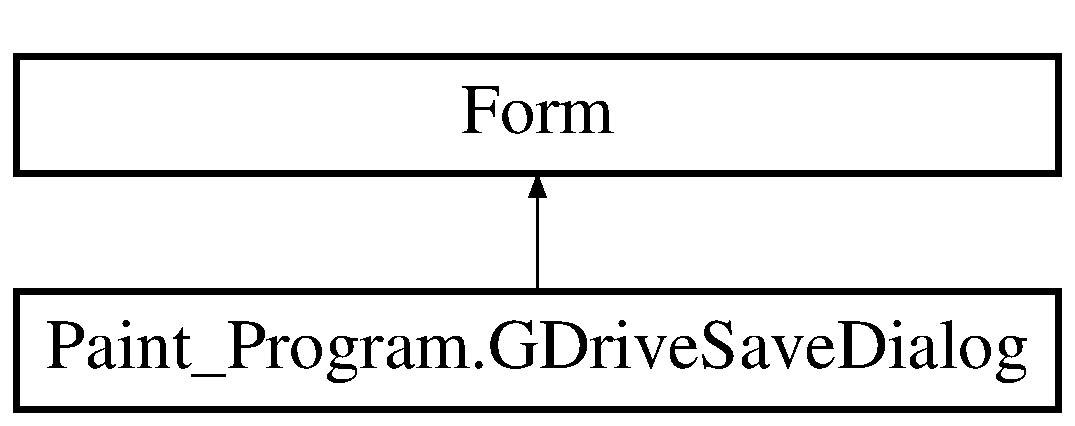
\includegraphics[height=2.000000cm]{class_paint___program_1_1_g_drive_save_dialog}
\end{center}
\end{figure}
\subsection*{Public Member Functions}
\begin{DoxyCompactItemize}
\item 
\mbox{\hyperlink{class_paint___program_1_1_g_drive_save_dialog_af0373baa9cc05fb6effe27ceb1f3063c}{G\+Drive\+Save\+Dialog}} ()
\end{DoxyCompactItemize}
\subsection*{Protected Member Functions}
\begin{DoxyCompactItemize}
\item 
override void \mbox{\hyperlink{class_paint___program_1_1_g_drive_save_dialog_ab6f349330bc5f3d3df824c7d1449ddc4}{Dispose}} (bool disposing)
\begin{DoxyCompactList}\small\item\em Clean up any resources being used. \end{DoxyCompactList}\end{DoxyCompactItemize}
\subsection*{Properties}
\begin{DoxyCompactItemize}
\item 
string \mbox{\hyperlink{class_paint___program_1_1_g_drive_save_dialog_a3cc969d8399b55a95fe053cdf11ce616}{file\+Name}}\hspace{0.3cm}{\ttfamily  \mbox{[}get, private set\mbox{]}}
\item 
string \mbox{\hyperlink{class_paint___program_1_1_g_drive_save_dialog_a7d92d2b564d15192cba1ecac3e2d0eea}{file\+Type}}\hspace{0.3cm}{\ttfamily  \mbox{[}get, private set\mbox{]}}
\end{DoxyCompactItemize}
\subsection*{Private Member Functions}
\begin{DoxyCompactItemize}
\item 
void \mbox{\hyperlink{class_paint___program_1_1_g_drive_save_dialog_a959f7a3b69241eb437b9f1a4fb85a78a}{btn\+\_\+save\+\_\+\+Click}} (object sender, Event\+Args e)
\item 
void \mbox{\hyperlink{class_paint___program_1_1_g_drive_save_dialog_ac5899bc01a3c230e5f584b4935e69bb6}{G\+Drive\+Save\+Dialog\+\_\+\+Key\+Down}} (object sender, Key\+Event\+Args e)
\item 
void \mbox{\hyperlink{class_paint___program_1_1_g_drive_save_dialog_af1ddb499fb44b4855723e4049430737a}{Initialize\+Component}} ()
\begin{DoxyCompactList}\small\item\em Required method for Designer support -\/ do not modify the contents of this method with the code editor. \end{DoxyCompactList}\end{DoxyCompactItemize}
\subsection*{Private Attributes}
\begin{DoxyCompactItemize}
\item 
System.\+Component\+Model.\+I\+Container \mbox{\hyperlink{class_paint___program_1_1_g_drive_save_dialog_a24fad5d02f8aabbc1c4cb44c589ea996}{components}} = null
\begin{DoxyCompactList}\small\item\em Required designer variable. \end{DoxyCompactList}\item 
System.\+Windows.\+Forms.\+Label \mbox{\hyperlink{class_paint___program_1_1_g_drive_save_dialog_a9e41e2aba62a97ccb2f503a292ba326b}{lbl\+\_\+\+File\+Name}}
\item 
System.\+Windows.\+Forms.\+Label \mbox{\hyperlink{class_paint___program_1_1_g_drive_save_dialog_a0246d2725477aee356db78f9310427dc}{lbl\+\_\+\+File\+Type}}
\item 
System.\+Windows.\+Forms.\+Text\+Box \mbox{\hyperlink{class_paint___program_1_1_g_drive_save_dialog_af9552fce325d995ecc4dc516416ea0d8}{tb\+\_\+\+File\+Name}}
\item 
System.\+Windows.\+Forms.\+Combo\+Box \mbox{\hyperlink{class_paint___program_1_1_g_drive_save_dialog_afb22d3b716cb3461399dbe7c6ac4b04c}{cb\+\_\+\+File\+Type}}
\item 
System.\+Windows.\+Forms.\+Button \mbox{\hyperlink{class_paint___program_1_1_g_drive_save_dialog_ac358c621a7f3820fd1298d40bbf581fe}{btn\+\_\+save}}
\end{DoxyCompactItemize}


\subsection{Constructor \& Destructor Documentation}
\mbox{\Hypertarget{class_paint___program_1_1_g_drive_save_dialog_af0373baa9cc05fb6effe27ceb1f3063c}\label{class_paint___program_1_1_g_drive_save_dialog_af0373baa9cc05fb6effe27ceb1f3063c}} 
\index{Paint\+\_\+\+Program\+::\+G\+Drive\+Save\+Dialog@{Paint\+\_\+\+Program\+::\+G\+Drive\+Save\+Dialog}!G\+Drive\+Save\+Dialog@{G\+Drive\+Save\+Dialog}}
\index{G\+Drive\+Save\+Dialog@{G\+Drive\+Save\+Dialog}!Paint\+\_\+\+Program\+::\+G\+Drive\+Save\+Dialog@{Paint\+\_\+\+Program\+::\+G\+Drive\+Save\+Dialog}}
\subsubsection{\texorpdfstring{G\+Drive\+Save\+Dialog()}{GDriveSaveDialog()}}
{\footnotesize\ttfamily Paint\+\_\+\+Program.\+G\+Drive\+Save\+Dialog.\+G\+Drive\+Save\+Dialog (\begin{DoxyParamCaption}{ }\end{DoxyParamCaption})\hspace{0.3cm}{\ttfamily [inline]}}



\subsection{Member Function Documentation}
\mbox{\Hypertarget{class_paint___program_1_1_g_drive_save_dialog_a959f7a3b69241eb437b9f1a4fb85a78a}\label{class_paint___program_1_1_g_drive_save_dialog_a959f7a3b69241eb437b9f1a4fb85a78a}} 
\index{Paint\+\_\+\+Program\+::\+G\+Drive\+Save\+Dialog@{Paint\+\_\+\+Program\+::\+G\+Drive\+Save\+Dialog}!btn\+\_\+save\+\_\+\+Click@{btn\+\_\+save\+\_\+\+Click}}
\index{btn\+\_\+save\+\_\+\+Click@{btn\+\_\+save\+\_\+\+Click}!Paint\+\_\+\+Program\+::\+G\+Drive\+Save\+Dialog@{Paint\+\_\+\+Program\+::\+G\+Drive\+Save\+Dialog}}
\subsubsection{\texorpdfstring{btn\+\_\+save\+\_\+\+Click()}{btn\_save\_Click()}}
{\footnotesize\ttfamily void Paint\+\_\+\+Program.\+G\+Drive\+Save\+Dialog.\+btn\+\_\+save\+\_\+\+Click (\begin{DoxyParamCaption}\item[{object}]{sender,  }\item[{Event\+Args}]{e }\end{DoxyParamCaption})\hspace{0.3cm}{\ttfamily [inline]}, {\ttfamily [private]}}

\mbox{\Hypertarget{class_paint___program_1_1_g_drive_save_dialog_ab6f349330bc5f3d3df824c7d1449ddc4}\label{class_paint___program_1_1_g_drive_save_dialog_ab6f349330bc5f3d3df824c7d1449ddc4}} 
\index{Paint\+\_\+\+Program\+::\+G\+Drive\+Save\+Dialog@{Paint\+\_\+\+Program\+::\+G\+Drive\+Save\+Dialog}!Dispose@{Dispose}}
\index{Dispose@{Dispose}!Paint\+\_\+\+Program\+::\+G\+Drive\+Save\+Dialog@{Paint\+\_\+\+Program\+::\+G\+Drive\+Save\+Dialog}}
\subsubsection{\texorpdfstring{Dispose()}{Dispose()}}
{\footnotesize\ttfamily override void Paint\+\_\+\+Program.\+G\+Drive\+Save\+Dialog.\+Dispose (\begin{DoxyParamCaption}\item[{bool}]{disposing }\end{DoxyParamCaption})\hspace{0.3cm}{\ttfamily [inline]}, {\ttfamily [protected]}}



Clean up any resources being used. 


\begin{DoxyParams}{Parameters}
{\em disposing} & true if managed resources should be disposed; otherwise, false.\\
\hline
\end{DoxyParams}
\mbox{\Hypertarget{class_paint___program_1_1_g_drive_save_dialog_ac5899bc01a3c230e5f584b4935e69bb6}\label{class_paint___program_1_1_g_drive_save_dialog_ac5899bc01a3c230e5f584b4935e69bb6}} 
\index{Paint\+\_\+\+Program\+::\+G\+Drive\+Save\+Dialog@{Paint\+\_\+\+Program\+::\+G\+Drive\+Save\+Dialog}!G\+Drive\+Save\+Dialog\+\_\+\+Key\+Down@{G\+Drive\+Save\+Dialog\+\_\+\+Key\+Down}}
\index{G\+Drive\+Save\+Dialog\+\_\+\+Key\+Down@{G\+Drive\+Save\+Dialog\+\_\+\+Key\+Down}!Paint\+\_\+\+Program\+::\+G\+Drive\+Save\+Dialog@{Paint\+\_\+\+Program\+::\+G\+Drive\+Save\+Dialog}}
\subsubsection{\texorpdfstring{G\+Drive\+Save\+Dialog\+\_\+\+Key\+Down()}{GDriveSaveDialog\_KeyDown()}}
{\footnotesize\ttfamily void Paint\+\_\+\+Program.\+G\+Drive\+Save\+Dialog.\+G\+Drive\+Save\+Dialog\+\_\+\+Key\+Down (\begin{DoxyParamCaption}\item[{object}]{sender,  }\item[{Key\+Event\+Args}]{e }\end{DoxyParamCaption})\hspace{0.3cm}{\ttfamily [inline]}, {\ttfamily [private]}}

\mbox{\Hypertarget{class_paint___program_1_1_g_drive_save_dialog_af1ddb499fb44b4855723e4049430737a}\label{class_paint___program_1_1_g_drive_save_dialog_af1ddb499fb44b4855723e4049430737a}} 
\index{Paint\+\_\+\+Program\+::\+G\+Drive\+Save\+Dialog@{Paint\+\_\+\+Program\+::\+G\+Drive\+Save\+Dialog}!Initialize\+Component@{Initialize\+Component}}
\index{Initialize\+Component@{Initialize\+Component}!Paint\+\_\+\+Program\+::\+G\+Drive\+Save\+Dialog@{Paint\+\_\+\+Program\+::\+G\+Drive\+Save\+Dialog}}
\subsubsection{\texorpdfstring{Initialize\+Component()}{InitializeComponent()}}
{\footnotesize\ttfamily void Paint\+\_\+\+Program.\+G\+Drive\+Save\+Dialog.\+Initialize\+Component (\begin{DoxyParamCaption}{ }\end{DoxyParamCaption})\hspace{0.3cm}{\ttfamily [inline]}, {\ttfamily [private]}}



Required method for Designer support -\/ do not modify the contents of this method with the code editor. 



\subsection{Member Data Documentation}
\mbox{\Hypertarget{class_paint___program_1_1_g_drive_save_dialog_ac358c621a7f3820fd1298d40bbf581fe}\label{class_paint___program_1_1_g_drive_save_dialog_ac358c621a7f3820fd1298d40bbf581fe}} 
\index{Paint\+\_\+\+Program\+::\+G\+Drive\+Save\+Dialog@{Paint\+\_\+\+Program\+::\+G\+Drive\+Save\+Dialog}!btn\+\_\+save@{btn\+\_\+save}}
\index{btn\+\_\+save@{btn\+\_\+save}!Paint\+\_\+\+Program\+::\+G\+Drive\+Save\+Dialog@{Paint\+\_\+\+Program\+::\+G\+Drive\+Save\+Dialog}}
\subsubsection{\texorpdfstring{btn\+\_\+save}{btn\_save}}
{\footnotesize\ttfamily System.\+Windows.\+Forms.\+Button Paint\+\_\+\+Program.\+G\+Drive\+Save\+Dialog.\+btn\+\_\+save\hspace{0.3cm}{\ttfamily [private]}}

\mbox{\Hypertarget{class_paint___program_1_1_g_drive_save_dialog_afb22d3b716cb3461399dbe7c6ac4b04c}\label{class_paint___program_1_1_g_drive_save_dialog_afb22d3b716cb3461399dbe7c6ac4b04c}} 
\index{Paint\+\_\+\+Program\+::\+G\+Drive\+Save\+Dialog@{Paint\+\_\+\+Program\+::\+G\+Drive\+Save\+Dialog}!cb\+\_\+\+File\+Type@{cb\+\_\+\+File\+Type}}
\index{cb\+\_\+\+File\+Type@{cb\+\_\+\+File\+Type}!Paint\+\_\+\+Program\+::\+G\+Drive\+Save\+Dialog@{Paint\+\_\+\+Program\+::\+G\+Drive\+Save\+Dialog}}
\subsubsection{\texorpdfstring{cb\+\_\+\+File\+Type}{cb\_FileType}}
{\footnotesize\ttfamily System.\+Windows.\+Forms.\+Combo\+Box Paint\+\_\+\+Program.\+G\+Drive\+Save\+Dialog.\+cb\+\_\+\+File\+Type\hspace{0.3cm}{\ttfamily [private]}}

\mbox{\Hypertarget{class_paint___program_1_1_g_drive_save_dialog_a24fad5d02f8aabbc1c4cb44c589ea996}\label{class_paint___program_1_1_g_drive_save_dialog_a24fad5d02f8aabbc1c4cb44c589ea996}} 
\index{Paint\+\_\+\+Program\+::\+G\+Drive\+Save\+Dialog@{Paint\+\_\+\+Program\+::\+G\+Drive\+Save\+Dialog}!components@{components}}
\index{components@{components}!Paint\+\_\+\+Program\+::\+G\+Drive\+Save\+Dialog@{Paint\+\_\+\+Program\+::\+G\+Drive\+Save\+Dialog}}
\subsubsection{\texorpdfstring{components}{components}}
{\footnotesize\ttfamily System.\+Component\+Model.\+I\+Container Paint\+\_\+\+Program.\+G\+Drive\+Save\+Dialog.\+components = null\hspace{0.3cm}{\ttfamily [private]}}



Required designer variable. 

\mbox{\Hypertarget{class_paint___program_1_1_g_drive_save_dialog_a9e41e2aba62a97ccb2f503a292ba326b}\label{class_paint___program_1_1_g_drive_save_dialog_a9e41e2aba62a97ccb2f503a292ba326b}} 
\index{Paint\+\_\+\+Program\+::\+G\+Drive\+Save\+Dialog@{Paint\+\_\+\+Program\+::\+G\+Drive\+Save\+Dialog}!lbl\+\_\+\+File\+Name@{lbl\+\_\+\+File\+Name}}
\index{lbl\+\_\+\+File\+Name@{lbl\+\_\+\+File\+Name}!Paint\+\_\+\+Program\+::\+G\+Drive\+Save\+Dialog@{Paint\+\_\+\+Program\+::\+G\+Drive\+Save\+Dialog}}
\subsubsection{\texorpdfstring{lbl\+\_\+\+File\+Name}{lbl\_FileName}}
{\footnotesize\ttfamily System.\+Windows.\+Forms.\+Label Paint\+\_\+\+Program.\+G\+Drive\+Save\+Dialog.\+lbl\+\_\+\+File\+Name\hspace{0.3cm}{\ttfamily [private]}}

\mbox{\Hypertarget{class_paint___program_1_1_g_drive_save_dialog_a0246d2725477aee356db78f9310427dc}\label{class_paint___program_1_1_g_drive_save_dialog_a0246d2725477aee356db78f9310427dc}} 
\index{Paint\+\_\+\+Program\+::\+G\+Drive\+Save\+Dialog@{Paint\+\_\+\+Program\+::\+G\+Drive\+Save\+Dialog}!lbl\+\_\+\+File\+Type@{lbl\+\_\+\+File\+Type}}
\index{lbl\+\_\+\+File\+Type@{lbl\+\_\+\+File\+Type}!Paint\+\_\+\+Program\+::\+G\+Drive\+Save\+Dialog@{Paint\+\_\+\+Program\+::\+G\+Drive\+Save\+Dialog}}
\subsubsection{\texorpdfstring{lbl\+\_\+\+File\+Type}{lbl\_FileType}}
{\footnotesize\ttfamily System.\+Windows.\+Forms.\+Label Paint\+\_\+\+Program.\+G\+Drive\+Save\+Dialog.\+lbl\+\_\+\+File\+Type\hspace{0.3cm}{\ttfamily [private]}}

\mbox{\Hypertarget{class_paint___program_1_1_g_drive_save_dialog_af9552fce325d995ecc4dc516416ea0d8}\label{class_paint___program_1_1_g_drive_save_dialog_af9552fce325d995ecc4dc516416ea0d8}} 
\index{Paint\+\_\+\+Program\+::\+G\+Drive\+Save\+Dialog@{Paint\+\_\+\+Program\+::\+G\+Drive\+Save\+Dialog}!tb\+\_\+\+File\+Name@{tb\+\_\+\+File\+Name}}
\index{tb\+\_\+\+File\+Name@{tb\+\_\+\+File\+Name}!Paint\+\_\+\+Program\+::\+G\+Drive\+Save\+Dialog@{Paint\+\_\+\+Program\+::\+G\+Drive\+Save\+Dialog}}
\subsubsection{\texorpdfstring{tb\+\_\+\+File\+Name}{tb\_FileName}}
{\footnotesize\ttfamily System.\+Windows.\+Forms.\+Text\+Box Paint\+\_\+\+Program.\+G\+Drive\+Save\+Dialog.\+tb\+\_\+\+File\+Name\hspace{0.3cm}{\ttfamily [private]}}



\subsection{Property Documentation}
\mbox{\Hypertarget{class_paint___program_1_1_g_drive_save_dialog_a3cc969d8399b55a95fe053cdf11ce616}\label{class_paint___program_1_1_g_drive_save_dialog_a3cc969d8399b55a95fe053cdf11ce616}} 
\index{Paint\+\_\+\+Program\+::\+G\+Drive\+Save\+Dialog@{Paint\+\_\+\+Program\+::\+G\+Drive\+Save\+Dialog}!file\+Name@{file\+Name}}
\index{file\+Name@{file\+Name}!Paint\+\_\+\+Program\+::\+G\+Drive\+Save\+Dialog@{Paint\+\_\+\+Program\+::\+G\+Drive\+Save\+Dialog}}
\subsubsection{\texorpdfstring{file\+Name}{fileName}}
{\footnotesize\ttfamily string Paint\+\_\+\+Program.\+G\+Drive\+Save\+Dialog.\+file\+Name\hspace{0.3cm}{\ttfamily [get]}, {\ttfamily [private set]}}

\mbox{\Hypertarget{class_paint___program_1_1_g_drive_save_dialog_a7d92d2b564d15192cba1ecac3e2d0eea}\label{class_paint___program_1_1_g_drive_save_dialog_a7d92d2b564d15192cba1ecac3e2d0eea}} 
\index{Paint\+\_\+\+Program\+::\+G\+Drive\+Save\+Dialog@{Paint\+\_\+\+Program\+::\+G\+Drive\+Save\+Dialog}!file\+Type@{file\+Type}}
\index{file\+Type@{file\+Type}!Paint\+\_\+\+Program\+::\+G\+Drive\+Save\+Dialog@{Paint\+\_\+\+Program\+::\+G\+Drive\+Save\+Dialog}}
\subsubsection{\texorpdfstring{file\+Type}{fileType}}
{\footnotesize\ttfamily string Paint\+\_\+\+Program.\+G\+Drive\+Save\+Dialog.\+file\+Type\hspace{0.3cm}{\ttfamily [get]}, {\ttfamily [private set]}}



The documentation for this class was generated from the following files\+:\begin{DoxyCompactItemize}
\item 
Paint Program/\mbox{\hyperlink{_g_drive_save_dialog_8cs}{G\+Drive\+Save\+Dialog.\+cs}}\item 
Paint Program/\mbox{\hyperlink{_g_drive_save_dialog_8_designer_8cs}{G\+Drive\+Save\+Dialog.\+Designer.\+cs}}\end{DoxyCompactItemize}

\hypertarget{class_paint___program_1_1_gif_encoder}{}\section{Paint\+\_\+\+Program.\+Gif\+Encoder Class Reference}
\label{class_paint___program_1_1_gif_encoder}\index{Paint\+\_\+\+Program.\+Gif\+Encoder@{Paint\+\_\+\+Program.\+Gif\+Encoder}}


Encodes multiple images as an animated gif to a stream. ~\newline
 A\+L\+W\+A\+YS A\+L\+W\+A\+YS A\+L\+W\+A\+YS wire this up in a using block ~\newline
 Disposing the encoder will complete the file. ~\newline
 Uses default .net G\+IF encoding and adds animation headers.  


Inheritance diagram for Paint\+\_\+\+Program.\+Gif\+Encoder\+:\begin{figure}[H]
\begin{center}
\leavevmode
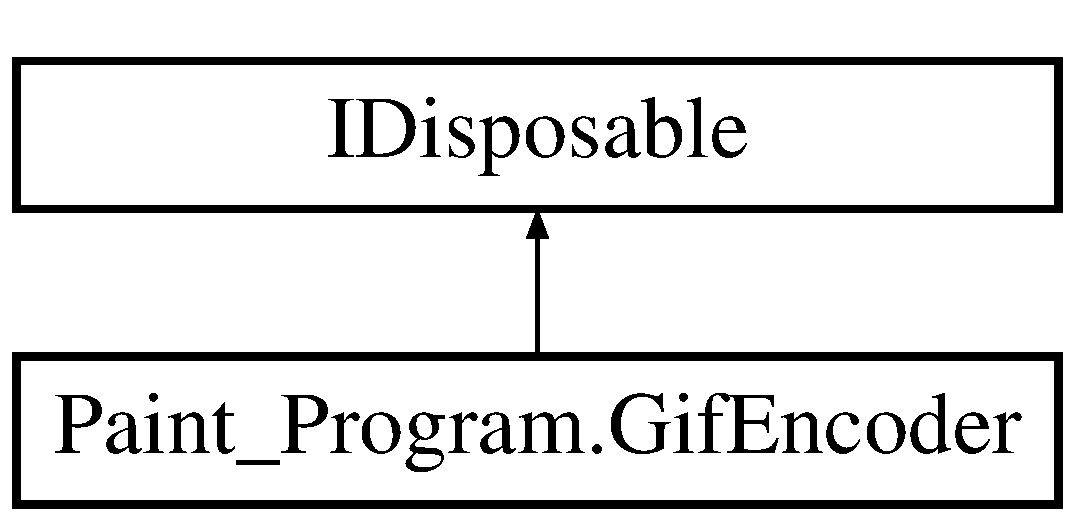
\includegraphics[height=2.000000cm]{class_paint___program_1_1_gif_encoder}
\end{center}
\end{figure}
\subsection*{Public Member Functions}
\begin{DoxyCompactItemize}
\item 
\mbox{\hyperlink{class_paint___program_1_1_gif_encoder_aa5dfacef849ac58b11453ced6cb559e2}{Gif\+Encoder}} (Stream stream, int? width=null, int? height=null, int? repeat\+Count=null)
\begin{DoxyCompactList}\small\item\em Encodes multiple images as an animated gif to a stream. ~\newline
 A\+L\+W\+A\+YS A\+L\+W\+A\+YS A\+L\+W\+A\+YS wire this in a using block ~\newline
 Disposing the encoder will complete the file. ~\newline
 Uses default .net G\+IF encoding and adds animation headers. \end{DoxyCompactList}\item 
void \mbox{\hyperlink{class_paint___program_1_1_gif_encoder_aac02f22617e5123c3101795ee3161d7f}{Add\+Frame}} (Image img, int x=0, int y=0, Time\+Span? frame\+Delay=null)
\begin{DoxyCompactList}\small\item\em Adds a frame to this animation. \end{DoxyCompactList}\item 
void \mbox{\hyperlink{class_paint___program_1_1_gif_encoder_a169050e40e9e0736b60337c2f3a4019b}{Dispose}} ()
\end{DoxyCompactItemize}
\subsection*{Properties}
\begin{DoxyCompactItemize}
\item 
Time\+Span \mbox{\hyperlink{class_paint___program_1_1_gif_encoder_af0a0f68f22ddcf8d84f2456adbc46165}{Frame\+Delay}}\hspace{0.3cm}{\ttfamily  \mbox{[}get, set\mbox{]}}
\end{DoxyCompactItemize}
\subsection*{Private Member Functions}
\begin{DoxyCompactItemize}
\item 
void \mbox{\hyperlink{class_paint___program_1_1_gif_encoder_abd4a3c3ab853d69be3551d16336cfe30}{Init\+Header}} (Stream source\+Gif, int w, int h)
\item 
void \mbox{\hyperlink{class_paint___program_1_1_gif_encoder_aab69513dafb7327f9decb3530313733e}{Write\+Color\+Table}} (Stream source\+Gif)
\item 
void \mbox{\hyperlink{class_paint___program_1_1_gif_encoder_aa549684b738eea97d7a00dd5df7bfe2e}{Write\+Graphic\+Control\+Block}} (Stream source\+Gif, Time\+Span frame\+Delay)
\item 
void \mbox{\hyperlink{class_paint___program_1_1_gif_encoder_a9668d36c48e46fd19a1679d442c2e228}{Write\+Image\+Block}} (Stream source\+Gif, bool include\+Color\+Table, int x, int y, int h, int w)
\item 
void \mbox{\hyperlink{class_paint___program_1_1_gif_encoder_a84c115c0609f30a5e20d4848400c8695}{Write\+Byte}} (int value)
\item 
void \mbox{\hyperlink{class_paint___program_1_1_gif_encoder_a64eb9e9108dbea9bf73e3ec0ca4e78fb}{Write\+Short}} (int value)
\item 
void \mbox{\hyperlink{class_paint___program_1_1_gif_encoder_a06fd85f8278561716c8dc37041d24497}{Write\+String}} (string value)
\end{DoxyCompactItemize}
\subsection*{Private Attributes}
\begin{DoxyCompactItemize}
\item 
const string \mbox{\hyperlink{class_paint___program_1_1_gif_encoder_a5b1c39cb88c56d947065736bc9132dd6}{File\+Type}} = \char`\"{}G\+IF\char`\"{}
\item 
const string \mbox{\hyperlink{class_paint___program_1_1_gif_encoder_ae87017427503b0b1abbad45b707e878e}{File\+Version}} = \char`\"{}89a\char`\"{}
\item 
const byte \mbox{\hyperlink{class_paint___program_1_1_gif_encoder_a057b20de45791f8e36a24c112507e187}{File\+Trailer}} = 0x3b
\item 
const int \mbox{\hyperlink{class_paint___program_1_1_gif_encoder_a7fd1aac1cf7f3fea28f0355fa2355dc6}{Application\+Extension\+Block\+Identifier}} = 0xff21
\item 
const byte \mbox{\hyperlink{class_paint___program_1_1_gif_encoder_ad7526c2ec09538fac4d99d51a4d80321}{Application\+Block\+Size}} = 0x0b
\item 
const string \mbox{\hyperlink{class_paint___program_1_1_gif_encoder_aa24cf121f9f2b444414c7da457edbb7d}{Application\+Identification}} = \char`\"{}N\+E\+T\+S\+C\+A\+P\+E2.\+0\char`\"{}
\item 
const int \mbox{\hyperlink{class_paint___program_1_1_gif_encoder_a8e5eaf58786b0ec4238a9c88fd87da85}{Graphic\+Control\+Extension\+Block\+Identifier}} = 0xf921
\item 
const byte \mbox{\hyperlink{class_paint___program_1_1_gif_encoder_a3076a85af102e60d670fd086f315e4a7}{Graphic\+Control\+Extension\+Block\+Size}} = 0x04
\item 
const long \mbox{\hyperlink{class_paint___program_1_1_gif_encoder_a147dfd6cf02f9cd9bb72e7b4638e4a28}{Source\+Global\+Color\+Info\+Position}} = 10
\item 
const long \mbox{\hyperlink{class_paint___program_1_1_gif_encoder_ac5a3d0830dde1a2094d797d97ad6498e}{Source\+Graphic\+Control\+Extension\+Position}} = 781
\item 
const long \mbox{\hyperlink{class_paint___program_1_1_gif_encoder_a01df6550b9828f02245ed2cd1072ca09}{Source\+Graphic\+Control\+Extension\+Length}} = 8
\item 
const long \mbox{\hyperlink{class_paint___program_1_1_gif_encoder_aadcfd603bed926d325615bebdbfd2cb3}{Source\+Image\+Block\+Position}} = 789
\item 
const long \mbox{\hyperlink{class_paint___program_1_1_gif_encoder_a1456c9cebb7e488514962743ac66d4cb}{Source\+Image\+Block\+Header\+Length}} = 11
\item 
const long \mbox{\hyperlink{class_paint___program_1_1_gif_encoder_a984a37788cb7c1ce3bd627a5a08e6e50}{Source\+Color\+Block\+Position}} = 13
\item 
const long \mbox{\hyperlink{class_paint___program_1_1_gif_encoder_a71eec2f591f9af7cb0b4d11d332df5a3}{Source\+Color\+Block\+Length}} = 768
\item 
bool \mbox{\hyperlink{class_paint___program_1_1_gif_encoder_a5de80ade0a9551f597da31f92b9d95eb}{\+\_\+is\+First\+Image}} = true
\item 
int \mbox{\hyperlink{class_paint___program_1_1_gif_encoder_a88e3a78c4e50284dcd716d73a8af55ae}{\+\_\+width}}
\item 
int \mbox{\hyperlink{class_paint___program_1_1_gif_encoder_a4f7b81f0b47ceffb51b3cfd7a1e32164}{\+\_\+height}}
\item 
int \mbox{\hyperlink{class_paint___program_1_1_gif_encoder_a238128613b44b86390393269f2768495}{\+\_\+repeat\+Count}}
\item 
readonly Stream \mbox{\hyperlink{class_paint___program_1_1_gif_encoder_a1b44df333c1ce4ebfebf59616352adf9}{\+\_\+stream}}
\end{DoxyCompactItemize}


\subsection{Detailed Description}
Encodes multiple images as an animated gif to a stream. ~\newline
 A\+L\+W\+A\+YS A\+L\+W\+A\+YS A\+L\+W\+A\+YS wire this up in a using block ~\newline
 Disposing the encoder will complete the file. ~\newline
 Uses default .net G\+IF encoding and adds animation headers. 



\subsection{Constructor \& Destructor Documentation}
\mbox{\Hypertarget{class_paint___program_1_1_gif_encoder_aa5dfacef849ac58b11453ced6cb559e2}\label{class_paint___program_1_1_gif_encoder_aa5dfacef849ac58b11453ced6cb559e2}} 
\index{Paint\+\_\+\+Program\+::\+Gif\+Encoder@{Paint\+\_\+\+Program\+::\+Gif\+Encoder}!Gif\+Encoder@{Gif\+Encoder}}
\index{Gif\+Encoder@{Gif\+Encoder}!Paint\+\_\+\+Program\+::\+Gif\+Encoder@{Paint\+\_\+\+Program\+::\+Gif\+Encoder}}
\subsubsection{\texorpdfstring{Gif\+Encoder()}{GifEncoder()}}
{\footnotesize\ttfamily Paint\+\_\+\+Program.\+Gif\+Encoder.\+Gif\+Encoder (\begin{DoxyParamCaption}\item[{Stream}]{stream,  }\item[{int?}]{width = {\ttfamily null},  }\item[{int?}]{height = {\ttfamily null},  }\item[{int?}]{repeat\+Count = {\ttfamily null} }\end{DoxyParamCaption})\hspace{0.3cm}{\ttfamily [inline]}}



Encodes multiple images as an animated gif to a stream. ~\newline
 A\+L\+W\+A\+YS A\+L\+W\+A\+YS A\+L\+W\+A\+YS wire this in a using block ~\newline
 Disposing the encoder will complete the file. ~\newline
 Uses default .net G\+IF encoding and adds animation headers. 


\begin{DoxyParams}{Parameters}
{\em stream} & The stream that will be written to.\\
\hline
{\em width} & Sets the width for this gif or null to use the first frame\textquotesingle{}s width.\\
\hline
{\em height} & Sets the height for this gif or null to use the first frame\textquotesingle{}s height.\\
\hline
\end{DoxyParams}


\subsection{Member Function Documentation}
\mbox{\Hypertarget{class_paint___program_1_1_gif_encoder_aac02f22617e5123c3101795ee3161d7f}\label{class_paint___program_1_1_gif_encoder_aac02f22617e5123c3101795ee3161d7f}} 
\index{Paint\+\_\+\+Program\+::\+Gif\+Encoder@{Paint\+\_\+\+Program\+::\+Gif\+Encoder}!Add\+Frame@{Add\+Frame}}
\index{Add\+Frame@{Add\+Frame}!Paint\+\_\+\+Program\+::\+Gif\+Encoder@{Paint\+\_\+\+Program\+::\+Gif\+Encoder}}
\subsubsection{\texorpdfstring{Add\+Frame()}{AddFrame()}}
{\footnotesize\ttfamily void Paint\+\_\+\+Program.\+Gif\+Encoder.\+Add\+Frame (\begin{DoxyParamCaption}\item[{Image}]{img,  }\item[{int}]{x = {\ttfamily 0},  }\item[{int}]{y = {\ttfamily 0},  }\item[{Time\+Span?}]{frame\+Delay = {\ttfamily null} }\end{DoxyParamCaption})\hspace{0.3cm}{\ttfamily [inline]}}



Adds a frame to this animation. 


\begin{DoxyParams}{Parameters}
{\em img} & The image to add\\
\hline
{\em x} & The positioning x offset this image should be displayed at.\\
\hline
{\em y} & The positioning y offset this image should be displayed at.\\
\hline
\end{DoxyParams}
\mbox{\Hypertarget{class_paint___program_1_1_gif_encoder_a169050e40e9e0736b60337c2f3a4019b}\label{class_paint___program_1_1_gif_encoder_a169050e40e9e0736b60337c2f3a4019b}} 
\index{Paint\+\_\+\+Program\+::\+Gif\+Encoder@{Paint\+\_\+\+Program\+::\+Gif\+Encoder}!Dispose@{Dispose}}
\index{Dispose@{Dispose}!Paint\+\_\+\+Program\+::\+Gif\+Encoder@{Paint\+\_\+\+Program\+::\+Gif\+Encoder}}
\subsubsection{\texorpdfstring{Dispose()}{Dispose()}}
{\footnotesize\ttfamily void Paint\+\_\+\+Program.\+Gif\+Encoder.\+Dispose (\begin{DoxyParamCaption}{ }\end{DoxyParamCaption})\hspace{0.3cm}{\ttfamily [inline]}}

\mbox{\Hypertarget{class_paint___program_1_1_gif_encoder_abd4a3c3ab853d69be3551d16336cfe30}\label{class_paint___program_1_1_gif_encoder_abd4a3c3ab853d69be3551d16336cfe30}} 
\index{Paint\+\_\+\+Program\+::\+Gif\+Encoder@{Paint\+\_\+\+Program\+::\+Gif\+Encoder}!Init\+Header@{Init\+Header}}
\index{Init\+Header@{Init\+Header}!Paint\+\_\+\+Program\+::\+Gif\+Encoder@{Paint\+\_\+\+Program\+::\+Gif\+Encoder}}
\subsubsection{\texorpdfstring{Init\+Header()}{InitHeader()}}
{\footnotesize\ttfamily void Paint\+\_\+\+Program.\+Gif\+Encoder.\+Init\+Header (\begin{DoxyParamCaption}\item[{Stream}]{source\+Gif,  }\item[{int}]{w,  }\item[{int}]{h }\end{DoxyParamCaption})\hspace{0.3cm}{\ttfamily [inline]}, {\ttfamily [private]}}

\mbox{\Hypertarget{class_paint___program_1_1_gif_encoder_a84c115c0609f30a5e20d4848400c8695}\label{class_paint___program_1_1_gif_encoder_a84c115c0609f30a5e20d4848400c8695}} 
\index{Paint\+\_\+\+Program\+::\+Gif\+Encoder@{Paint\+\_\+\+Program\+::\+Gif\+Encoder}!Write\+Byte@{Write\+Byte}}
\index{Write\+Byte@{Write\+Byte}!Paint\+\_\+\+Program\+::\+Gif\+Encoder@{Paint\+\_\+\+Program\+::\+Gif\+Encoder}}
\subsubsection{\texorpdfstring{Write\+Byte()}{WriteByte()}}
{\footnotesize\ttfamily void Paint\+\_\+\+Program.\+Gif\+Encoder.\+Write\+Byte (\begin{DoxyParamCaption}\item[{int}]{value }\end{DoxyParamCaption})\hspace{0.3cm}{\ttfamily [inline]}, {\ttfamily [private]}}

\mbox{\Hypertarget{class_paint___program_1_1_gif_encoder_aab69513dafb7327f9decb3530313733e}\label{class_paint___program_1_1_gif_encoder_aab69513dafb7327f9decb3530313733e}} 
\index{Paint\+\_\+\+Program\+::\+Gif\+Encoder@{Paint\+\_\+\+Program\+::\+Gif\+Encoder}!Write\+Color\+Table@{Write\+Color\+Table}}
\index{Write\+Color\+Table@{Write\+Color\+Table}!Paint\+\_\+\+Program\+::\+Gif\+Encoder@{Paint\+\_\+\+Program\+::\+Gif\+Encoder}}
\subsubsection{\texorpdfstring{Write\+Color\+Table()}{WriteColorTable()}}
{\footnotesize\ttfamily void Paint\+\_\+\+Program.\+Gif\+Encoder.\+Write\+Color\+Table (\begin{DoxyParamCaption}\item[{Stream}]{source\+Gif }\end{DoxyParamCaption})\hspace{0.3cm}{\ttfamily [inline]}, {\ttfamily [private]}}

\mbox{\Hypertarget{class_paint___program_1_1_gif_encoder_aa549684b738eea97d7a00dd5df7bfe2e}\label{class_paint___program_1_1_gif_encoder_aa549684b738eea97d7a00dd5df7bfe2e}} 
\index{Paint\+\_\+\+Program\+::\+Gif\+Encoder@{Paint\+\_\+\+Program\+::\+Gif\+Encoder}!Write\+Graphic\+Control\+Block@{Write\+Graphic\+Control\+Block}}
\index{Write\+Graphic\+Control\+Block@{Write\+Graphic\+Control\+Block}!Paint\+\_\+\+Program\+::\+Gif\+Encoder@{Paint\+\_\+\+Program\+::\+Gif\+Encoder}}
\subsubsection{\texorpdfstring{Write\+Graphic\+Control\+Block()}{WriteGraphicControlBlock()}}
{\footnotesize\ttfamily void Paint\+\_\+\+Program.\+Gif\+Encoder.\+Write\+Graphic\+Control\+Block (\begin{DoxyParamCaption}\item[{Stream}]{source\+Gif,  }\item[{Time\+Span}]{frame\+Delay }\end{DoxyParamCaption})\hspace{0.3cm}{\ttfamily [inline]}, {\ttfamily [private]}}

\mbox{\Hypertarget{class_paint___program_1_1_gif_encoder_a9668d36c48e46fd19a1679d442c2e228}\label{class_paint___program_1_1_gif_encoder_a9668d36c48e46fd19a1679d442c2e228}} 
\index{Paint\+\_\+\+Program\+::\+Gif\+Encoder@{Paint\+\_\+\+Program\+::\+Gif\+Encoder}!Write\+Image\+Block@{Write\+Image\+Block}}
\index{Write\+Image\+Block@{Write\+Image\+Block}!Paint\+\_\+\+Program\+::\+Gif\+Encoder@{Paint\+\_\+\+Program\+::\+Gif\+Encoder}}
\subsubsection{\texorpdfstring{Write\+Image\+Block()}{WriteImageBlock()}}
{\footnotesize\ttfamily void Paint\+\_\+\+Program.\+Gif\+Encoder.\+Write\+Image\+Block (\begin{DoxyParamCaption}\item[{Stream}]{source\+Gif,  }\item[{bool}]{include\+Color\+Table,  }\item[{int}]{x,  }\item[{int}]{y,  }\item[{int}]{h,  }\item[{int}]{w }\end{DoxyParamCaption})\hspace{0.3cm}{\ttfamily [inline]}, {\ttfamily [private]}}

\mbox{\Hypertarget{class_paint___program_1_1_gif_encoder_a64eb9e9108dbea9bf73e3ec0ca4e78fb}\label{class_paint___program_1_1_gif_encoder_a64eb9e9108dbea9bf73e3ec0ca4e78fb}} 
\index{Paint\+\_\+\+Program\+::\+Gif\+Encoder@{Paint\+\_\+\+Program\+::\+Gif\+Encoder}!Write\+Short@{Write\+Short}}
\index{Write\+Short@{Write\+Short}!Paint\+\_\+\+Program\+::\+Gif\+Encoder@{Paint\+\_\+\+Program\+::\+Gif\+Encoder}}
\subsubsection{\texorpdfstring{Write\+Short()}{WriteShort()}}
{\footnotesize\ttfamily void Paint\+\_\+\+Program.\+Gif\+Encoder.\+Write\+Short (\begin{DoxyParamCaption}\item[{int}]{value }\end{DoxyParamCaption})\hspace{0.3cm}{\ttfamily [inline]}, {\ttfamily [private]}}

\mbox{\Hypertarget{class_paint___program_1_1_gif_encoder_a06fd85f8278561716c8dc37041d24497}\label{class_paint___program_1_1_gif_encoder_a06fd85f8278561716c8dc37041d24497}} 
\index{Paint\+\_\+\+Program\+::\+Gif\+Encoder@{Paint\+\_\+\+Program\+::\+Gif\+Encoder}!Write\+String@{Write\+String}}
\index{Write\+String@{Write\+String}!Paint\+\_\+\+Program\+::\+Gif\+Encoder@{Paint\+\_\+\+Program\+::\+Gif\+Encoder}}
\subsubsection{\texorpdfstring{Write\+String()}{WriteString()}}
{\footnotesize\ttfamily void Paint\+\_\+\+Program.\+Gif\+Encoder.\+Write\+String (\begin{DoxyParamCaption}\item[{string}]{value }\end{DoxyParamCaption})\hspace{0.3cm}{\ttfamily [inline]}, {\ttfamily [private]}}



\subsection{Member Data Documentation}
\mbox{\Hypertarget{class_paint___program_1_1_gif_encoder_a4f7b81f0b47ceffb51b3cfd7a1e32164}\label{class_paint___program_1_1_gif_encoder_a4f7b81f0b47ceffb51b3cfd7a1e32164}} 
\index{Paint\+\_\+\+Program\+::\+Gif\+Encoder@{Paint\+\_\+\+Program\+::\+Gif\+Encoder}!\+\_\+height@{\+\_\+height}}
\index{\+\_\+height@{\+\_\+height}!Paint\+\_\+\+Program\+::\+Gif\+Encoder@{Paint\+\_\+\+Program\+::\+Gif\+Encoder}}
\subsubsection{\texorpdfstring{\+\_\+height}{\_height}}
{\footnotesize\ttfamily int Paint\+\_\+\+Program.\+Gif\+Encoder.\+\_\+height\hspace{0.3cm}{\ttfamily [private]}}

\mbox{\Hypertarget{class_paint___program_1_1_gif_encoder_a5de80ade0a9551f597da31f92b9d95eb}\label{class_paint___program_1_1_gif_encoder_a5de80ade0a9551f597da31f92b9d95eb}} 
\index{Paint\+\_\+\+Program\+::\+Gif\+Encoder@{Paint\+\_\+\+Program\+::\+Gif\+Encoder}!\+\_\+is\+First\+Image@{\+\_\+is\+First\+Image}}
\index{\+\_\+is\+First\+Image@{\+\_\+is\+First\+Image}!Paint\+\_\+\+Program\+::\+Gif\+Encoder@{Paint\+\_\+\+Program\+::\+Gif\+Encoder}}
\subsubsection{\texorpdfstring{\+\_\+is\+First\+Image}{\_isFirstImage}}
{\footnotesize\ttfamily bool Paint\+\_\+\+Program.\+Gif\+Encoder.\+\_\+is\+First\+Image = true\hspace{0.3cm}{\ttfamily [private]}}

\mbox{\Hypertarget{class_paint___program_1_1_gif_encoder_a238128613b44b86390393269f2768495}\label{class_paint___program_1_1_gif_encoder_a238128613b44b86390393269f2768495}} 
\index{Paint\+\_\+\+Program\+::\+Gif\+Encoder@{Paint\+\_\+\+Program\+::\+Gif\+Encoder}!\+\_\+repeat\+Count@{\+\_\+repeat\+Count}}
\index{\+\_\+repeat\+Count@{\+\_\+repeat\+Count}!Paint\+\_\+\+Program\+::\+Gif\+Encoder@{Paint\+\_\+\+Program\+::\+Gif\+Encoder}}
\subsubsection{\texorpdfstring{\+\_\+repeat\+Count}{\_repeatCount}}
{\footnotesize\ttfamily int Paint\+\_\+\+Program.\+Gif\+Encoder.\+\_\+repeat\+Count\hspace{0.3cm}{\ttfamily [private]}}

\mbox{\Hypertarget{class_paint___program_1_1_gif_encoder_a1b44df333c1ce4ebfebf59616352adf9}\label{class_paint___program_1_1_gif_encoder_a1b44df333c1ce4ebfebf59616352adf9}} 
\index{Paint\+\_\+\+Program\+::\+Gif\+Encoder@{Paint\+\_\+\+Program\+::\+Gif\+Encoder}!\+\_\+stream@{\+\_\+stream}}
\index{\+\_\+stream@{\+\_\+stream}!Paint\+\_\+\+Program\+::\+Gif\+Encoder@{Paint\+\_\+\+Program\+::\+Gif\+Encoder}}
\subsubsection{\texorpdfstring{\+\_\+stream}{\_stream}}
{\footnotesize\ttfamily readonly Stream Paint\+\_\+\+Program.\+Gif\+Encoder.\+\_\+stream\hspace{0.3cm}{\ttfamily [private]}}

\mbox{\Hypertarget{class_paint___program_1_1_gif_encoder_a88e3a78c4e50284dcd716d73a8af55ae}\label{class_paint___program_1_1_gif_encoder_a88e3a78c4e50284dcd716d73a8af55ae}} 
\index{Paint\+\_\+\+Program\+::\+Gif\+Encoder@{Paint\+\_\+\+Program\+::\+Gif\+Encoder}!\+\_\+width@{\+\_\+width}}
\index{\+\_\+width@{\+\_\+width}!Paint\+\_\+\+Program\+::\+Gif\+Encoder@{Paint\+\_\+\+Program\+::\+Gif\+Encoder}}
\subsubsection{\texorpdfstring{\+\_\+width}{\_width}}
{\footnotesize\ttfamily int Paint\+\_\+\+Program.\+Gif\+Encoder.\+\_\+width\hspace{0.3cm}{\ttfamily [private]}}

\mbox{\Hypertarget{class_paint___program_1_1_gif_encoder_ad7526c2ec09538fac4d99d51a4d80321}\label{class_paint___program_1_1_gif_encoder_ad7526c2ec09538fac4d99d51a4d80321}} 
\index{Paint\+\_\+\+Program\+::\+Gif\+Encoder@{Paint\+\_\+\+Program\+::\+Gif\+Encoder}!Application\+Block\+Size@{Application\+Block\+Size}}
\index{Application\+Block\+Size@{Application\+Block\+Size}!Paint\+\_\+\+Program\+::\+Gif\+Encoder@{Paint\+\_\+\+Program\+::\+Gif\+Encoder}}
\subsubsection{\texorpdfstring{Application\+Block\+Size}{ApplicationBlockSize}}
{\footnotesize\ttfamily const byte Paint\+\_\+\+Program.\+Gif\+Encoder.\+Application\+Block\+Size = 0x0b\hspace{0.3cm}{\ttfamily [private]}}

\mbox{\Hypertarget{class_paint___program_1_1_gif_encoder_a7fd1aac1cf7f3fea28f0355fa2355dc6}\label{class_paint___program_1_1_gif_encoder_a7fd1aac1cf7f3fea28f0355fa2355dc6}} 
\index{Paint\+\_\+\+Program\+::\+Gif\+Encoder@{Paint\+\_\+\+Program\+::\+Gif\+Encoder}!Application\+Extension\+Block\+Identifier@{Application\+Extension\+Block\+Identifier}}
\index{Application\+Extension\+Block\+Identifier@{Application\+Extension\+Block\+Identifier}!Paint\+\_\+\+Program\+::\+Gif\+Encoder@{Paint\+\_\+\+Program\+::\+Gif\+Encoder}}
\subsubsection{\texorpdfstring{Application\+Extension\+Block\+Identifier}{ApplicationExtensionBlockIdentifier}}
{\footnotesize\ttfamily const int Paint\+\_\+\+Program.\+Gif\+Encoder.\+Application\+Extension\+Block\+Identifier = 0xff21\hspace{0.3cm}{\ttfamily [private]}}

\mbox{\Hypertarget{class_paint___program_1_1_gif_encoder_aa24cf121f9f2b444414c7da457edbb7d}\label{class_paint___program_1_1_gif_encoder_aa24cf121f9f2b444414c7da457edbb7d}} 
\index{Paint\+\_\+\+Program\+::\+Gif\+Encoder@{Paint\+\_\+\+Program\+::\+Gif\+Encoder}!Application\+Identification@{Application\+Identification}}
\index{Application\+Identification@{Application\+Identification}!Paint\+\_\+\+Program\+::\+Gif\+Encoder@{Paint\+\_\+\+Program\+::\+Gif\+Encoder}}
\subsubsection{\texorpdfstring{Application\+Identification}{ApplicationIdentification}}
{\footnotesize\ttfamily const string Paint\+\_\+\+Program.\+Gif\+Encoder.\+Application\+Identification = \char`\"{}N\+E\+T\+S\+C\+A\+P\+E2.\+0\char`\"{}\hspace{0.3cm}{\ttfamily [private]}}

\mbox{\Hypertarget{class_paint___program_1_1_gif_encoder_a057b20de45791f8e36a24c112507e187}\label{class_paint___program_1_1_gif_encoder_a057b20de45791f8e36a24c112507e187}} 
\index{Paint\+\_\+\+Program\+::\+Gif\+Encoder@{Paint\+\_\+\+Program\+::\+Gif\+Encoder}!File\+Trailer@{File\+Trailer}}
\index{File\+Trailer@{File\+Trailer}!Paint\+\_\+\+Program\+::\+Gif\+Encoder@{Paint\+\_\+\+Program\+::\+Gif\+Encoder}}
\subsubsection{\texorpdfstring{File\+Trailer}{FileTrailer}}
{\footnotesize\ttfamily const byte Paint\+\_\+\+Program.\+Gif\+Encoder.\+File\+Trailer = 0x3b\hspace{0.3cm}{\ttfamily [private]}}

\mbox{\Hypertarget{class_paint___program_1_1_gif_encoder_a5b1c39cb88c56d947065736bc9132dd6}\label{class_paint___program_1_1_gif_encoder_a5b1c39cb88c56d947065736bc9132dd6}} 
\index{Paint\+\_\+\+Program\+::\+Gif\+Encoder@{Paint\+\_\+\+Program\+::\+Gif\+Encoder}!File\+Type@{File\+Type}}
\index{File\+Type@{File\+Type}!Paint\+\_\+\+Program\+::\+Gif\+Encoder@{Paint\+\_\+\+Program\+::\+Gif\+Encoder}}
\subsubsection{\texorpdfstring{File\+Type}{FileType}}
{\footnotesize\ttfamily const string Paint\+\_\+\+Program.\+Gif\+Encoder.\+File\+Type = \char`\"{}G\+IF\char`\"{}\hspace{0.3cm}{\ttfamily [private]}}

\mbox{\Hypertarget{class_paint___program_1_1_gif_encoder_ae87017427503b0b1abbad45b707e878e}\label{class_paint___program_1_1_gif_encoder_ae87017427503b0b1abbad45b707e878e}} 
\index{Paint\+\_\+\+Program\+::\+Gif\+Encoder@{Paint\+\_\+\+Program\+::\+Gif\+Encoder}!File\+Version@{File\+Version}}
\index{File\+Version@{File\+Version}!Paint\+\_\+\+Program\+::\+Gif\+Encoder@{Paint\+\_\+\+Program\+::\+Gif\+Encoder}}
\subsubsection{\texorpdfstring{File\+Version}{FileVersion}}
{\footnotesize\ttfamily const string Paint\+\_\+\+Program.\+Gif\+Encoder.\+File\+Version = \char`\"{}89a\char`\"{}\hspace{0.3cm}{\ttfamily [private]}}

\mbox{\Hypertarget{class_paint___program_1_1_gif_encoder_a8e5eaf58786b0ec4238a9c88fd87da85}\label{class_paint___program_1_1_gif_encoder_a8e5eaf58786b0ec4238a9c88fd87da85}} 
\index{Paint\+\_\+\+Program\+::\+Gif\+Encoder@{Paint\+\_\+\+Program\+::\+Gif\+Encoder}!Graphic\+Control\+Extension\+Block\+Identifier@{Graphic\+Control\+Extension\+Block\+Identifier}}
\index{Graphic\+Control\+Extension\+Block\+Identifier@{Graphic\+Control\+Extension\+Block\+Identifier}!Paint\+\_\+\+Program\+::\+Gif\+Encoder@{Paint\+\_\+\+Program\+::\+Gif\+Encoder}}
\subsubsection{\texorpdfstring{Graphic\+Control\+Extension\+Block\+Identifier}{GraphicControlExtensionBlockIdentifier}}
{\footnotesize\ttfamily const int Paint\+\_\+\+Program.\+Gif\+Encoder.\+Graphic\+Control\+Extension\+Block\+Identifier = 0xf921\hspace{0.3cm}{\ttfamily [private]}}

\mbox{\Hypertarget{class_paint___program_1_1_gif_encoder_a3076a85af102e60d670fd086f315e4a7}\label{class_paint___program_1_1_gif_encoder_a3076a85af102e60d670fd086f315e4a7}} 
\index{Paint\+\_\+\+Program\+::\+Gif\+Encoder@{Paint\+\_\+\+Program\+::\+Gif\+Encoder}!Graphic\+Control\+Extension\+Block\+Size@{Graphic\+Control\+Extension\+Block\+Size}}
\index{Graphic\+Control\+Extension\+Block\+Size@{Graphic\+Control\+Extension\+Block\+Size}!Paint\+\_\+\+Program\+::\+Gif\+Encoder@{Paint\+\_\+\+Program\+::\+Gif\+Encoder}}
\subsubsection{\texorpdfstring{Graphic\+Control\+Extension\+Block\+Size}{GraphicControlExtensionBlockSize}}
{\footnotesize\ttfamily const byte Paint\+\_\+\+Program.\+Gif\+Encoder.\+Graphic\+Control\+Extension\+Block\+Size = 0x04\hspace{0.3cm}{\ttfamily [private]}}

\mbox{\Hypertarget{class_paint___program_1_1_gif_encoder_a71eec2f591f9af7cb0b4d11d332df5a3}\label{class_paint___program_1_1_gif_encoder_a71eec2f591f9af7cb0b4d11d332df5a3}} 
\index{Paint\+\_\+\+Program\+::\+Gif\+Encoder@{Paint\+\_\+\+Program\+::\+Gif\+Encoder}!Source\+Color\+Block\+Length@{Source\+Color\+Block\+Length}}
\index{Source\+Color\+Block\+Length@{Source\+Color\+Block\+Length}!Paint\+\_\+\+Program\+::\+Gif\+Encoder@{Paint\+\_\+\+Program\+::\+Gif\+Encoder}}
\subsubsection{\texorpdfstring{Source\+Color\+Block\+Length}{SourceColorBlockLength}}
{\footnotesize\ttfamily const long Paint\+\_\+\+Program.\+Gif\+Encoder.\+Source\+Color\+Block\+Length = 768\hspace{0.3cm}{\ttfamily [private]}}

\mbox{\Hypertarget{class_paint___program_1_1_gif_encoder_a984a37788cb7c1ce3bd627a5a08e6e50}\label{class_paint___program_1_1_gif_encoder_a984a37788cb7c1ce3bd627a5a08e6e50}} 
\index{Paint\+\_\+\+Program\+::\+Gif\+Encoder@{Paint\+\_\+\+Program\+::\+Gif\+Encoder}!Source\+Color\+Block\+Position@{Source\+Color\+Block\+Position}}
\index{Source\+Color\+Block\+Position@{Source\+Color\+Block\+Position}!Paint\+\_\+\+Program\+::\+Gif\+Encoder@{Paint\+\_\+\+Program\+::\+Gif\+Encoder}}
\subsubsection{\texorpdfstring{Source\+Color\+Block\+Position}{SourceColorBlockPosition}}
{\footnotesize\ttfamily const long Paint\+\_\+\+Program.\+Gif\+Encoder.\+Source\+Color\+Block\+Position = 13\hspace{0.3cm}{\ttfamily [private]}}

\mbox{\Hypertarget{class_paint___program_1_1_gif_encoder_a147dfd6cf02f9cd9bb72e7b4638e4a28}\label{class_paint___program_1_1_gif_encoder_a147dfd6cf02f9cd9bb72e7b4638e4a28}} 
\index{Paint\+\_\+\+Program\+::\+Gif\+Encoder@{Paint\+\_\+\+Program\+::\+Gif\+Encoder}!Source\+Global\+Color\+Info\+Position@{Source\+Global\+Color\+Info\+Position}}
\index{Source\+Global\+Color\+Info\+Position@{Source\+Global\+Color\+Info\+Position}!Paint\+\_\+\+Program\+::\+Gif\+Encoder@{Paint\+\_\+\+Program\+::\+Gif\+Encoder}}
\subsubsection{\texorpdfstring{Source\+Global\+Color\+Info\+Position}{SourceGlobalColorInfoPosition}}
{\footnotesize\ttfamily const long Paint\+\_\+\+Program.\+Gif\+Encoder.\+Source\+Global\+Color\+Info\+Position = 10\hspace{0.3cm}{\ttfamily [private]}}

\mbox{\Hypertarget{class_paint___program_1_1_gif_encoder_a01df6550b9828f02245ed2cd1072ca09}\label{class_paint___program_1_1_gif_encoder_a01df6550b9828f02245ed2cd1072ca09}} 
\index{Paint\+\_\+\+Program\+::\+Gif\+Encoder@{Paint\+\_\+\+Program\+::\+Gif\+Encoder}!Source\+Graphic\+Control\+Extension\+Length@{Source\+Graphic\+Control\+Extension\+Length}}
\index{Source\+Graphic\+Control\+Extension\+Length@{Source\+Graphic\+Control\+Extension\+Length}!Paint\+\_\+\+Program\+::\+Gif\+Encoder@{Paint\+\_\+\+Program\+::\+Gif\+Encoder}}
\subsubsection{\texorpdfstring{Source\+Graphic\+Control\+Extension\+Length}{SourceGraphicControlExtensionLength}}
{\footnotesize\ttfamily const long Paint\+\_\+\+Program.\+Gif\+Encoder.\+Source\+Graphic\+Control\+Extension\+Length = 8\hspace{0.3cm}{\ttfamily [private]}}

\mbox{\Hypertarget{class_paint___program_1_1_gif_encoder_ac5a3d0830dde1a2094d797d97ad6498e}\label{class_paint___program_1_1_gif_encoder_ac5a3d0830dde1a2094d797d97ad6498e}} 
\index{Paint\+\_\+\+Program\+::\+Gif\+Encoder@{Paint\+\_\+\+Program\+::\+Gif\+Encoder}!Source\+Graphic\+Control\+Extension\+Position@{Source\+Graphic\+Control\+Extension\+Position}}
\index{Source\+Graphic\+Control\+Extension\+Position@{Source\+Graphic\+Control\+Extension\+Position}!Paint\+\_\+\+Program\+::\+Gif\+Encoder@{Paint\+\_\+\+Program\+::\+Gif\+Encoder}}
\subsubsection{\texorpdfstring{Source\+Graphic\+Control\+Extension\+Position}{SourceGraphicControlExtensionPosition}}
{\footnotesize\ttfamily const long Paint\+\_\+\+Program.\+Gif\+Encoder.\+Source\+Graphic\+Control\+Extension\+Position = 781\hspace{0.3cm}{\ttfamily [private]}}

\mbox{\Hypertarget{class_paint___program_1_1_gif_encoder_a1456c9cebb7e488514962743ac66d4cb}\label{class_paint___program_1_1_gif_encoder_a1456c9cebb7e488514962743ac66d4cb}} 
\index{Paint\+\_\+\+Program\+::\+Gif\+Encoder@{Paint\+\_\+\+Program\+::\+Gif\+Encoder}!Source\+Image\+Block\+Header\+Length@{Source\+Image\+Block\+Header\+Length}}
\index{Source\+Image\+Block\+Header\+Length@{Source\+Image\+Block\+Header\+Length}!Paint\+\_\+\+Program\+::\+Gif\+Encoder@{Paint\+\_\+\+Program\+::\+Gif\+Encoder}}
\subsubsection{\texorpdfstring{Source\+Image\+Block\+Header\+Length}{SourceImageBlockHeaderLength}}
{\footnotesize\ttfamily const long Paint\+\_\+\+Program.\+Gif\+Encoder.\+Source\+Image\+Block\+Header\+Length = 11\hspace{0.3cm}{\ttfamily [private]}}

\mbox{\Hypertarget{class_paint___program_1_1_gif_encoder_aadcfd603bed926d325615bebdbfd2cb3}\label{class_paint___program_1_1_gif_encoder_aadcfd603bed926d325615bebdbfd2cb3}} 
\index{Paint\+\_\+\+Program\+::\+Gif\+Encoder@{Paint\+\_\+\+Program\+::\+Gif\+Encoder}!Source\+Image\+Block\+Position@{Source\+Image\+Block\+Position}}
\index{Source\+Image\+Block\+Position@{Source\+Image\+Block\+Position}!Paint\+\_\+\+Program\+::\+Gif\+Encoder@{Paint\+\_\+\+Program\+::\+Gif\+Encoder}}
\subsubsection{\texorpdfstring{Source\+Image\+Block\+Position}{SourceImageBlockPosition}}
{\footnotesize\ttfamily const long Paint\+\_\+\+Program.\+Gif\+Encoder.\+Source\+Image\+Block\+Position = 789\hspace{0.3cm}{\ttfamily [private]}}



\subsection{Property Documentation}
\mbox{\Hypertarget{class_paint___program_1_1_gif_encoder_af0a0f68f22ddcf8d84f2456adbc46165}\label{class_paint___program_1_1_gif_encoder_af0a0f68f22ddcf8d84f2456adbc46165}} 
\index{Paint\+\_\+\+Program\+::\+Gif\+Encoder@{Paint\+\_\+\+Program\+::\+Gif\+Encoder}!Frame\+Delay@{Frame\+Delay}}
\index{Frame\+Delay@{Frame\+Delay}!Paint\+\_\+\+Program\+::\+Gif\+Encoder@{Paint\+\_\+\+Program\+::\+Gif\+Encoder}}
\subsubsection{\texorpdfstring{Frame\+Delay}{FrameDelay}}
{\footnotesize\ttfamily Time\+Span Paint\+\_\+\+Program.\+Gif\+Encoder.\+Frame\+Delay\hspace{0.3cm}{\ttfamily [get]}, {\ttfamily [set]}}



The documentation for this class was generated from the following file\+:\begin{DoxyCompactItemize}
\item 
Paint Program/\mbox{\hyperlink{_gif_encoder_8cs}{Gif\+Encoder.\+cs}}\end{DoxyCompactItemize}

\hypertarget{class_paint___program_1_1_google_drive_upload}{}\section{Paint\+\_\+\+Program.\+Google\+Drive\+Upload Class Reference}
\label{class_paint___program_1_1_google_drive_upload}\index{Paint\+\_\+\+Program.\+Google\+Drive\+Upload@{Paint\+\_\+\+Program.\+Google\+Drive\+Upload}}
\subsection*{Static Public Member Functions}
\begin{DoxyCompactItemize}
\item 
static void \mbox{\hyperlink{class_paint___program_1_1_google_drive_upload_afd2b70d90c0c3a412f9c2f11d0c63f99}{Drive\+Upload}} (string path\+To\+File)
\end{DoxyCompactItemize}
\subsection*{Static Private Member Functions}
\begin{DoxyCompactItemize}
\item 
static string \mbox{\hyperlink{class_paint___program_1_1_google_drive_upload_aa3a741d118b7e3b4cb17ad5f1a871201}{Get\+Mime\+Type}} (string file\+Name)
\end{DoxyCompactItemize}
\subsection*{Static Private Attributes}
\begin{DoxyCompactItemize}
\item 
static string \mbox{[}$\,$\mbox{]} \mbox{\hyperlink{class_paint___program_1_1_google_drive_upload_aa60a9c9a8dd82f038fe5fbb247fc5c38}{Scopes}} = \{ Drive\+Service.\+Scope.\+Drive \}
\item 
static string \mbox{\hyperlink{class_paint___program_1_1_google_drive_upload_a20c7374606e9a10898d08f487a4d5319}{Application\+Name}} = \char`\"{}Le\+Paint\char`\"{}
\end{DoxyCompactItemize}


\subsection{Member Function Documentation}
\mbox{\Hypertarget{class_paint___program_1_1_google_drive_upload_afd2b70d90c0c3a412f9c2f11d0c63f99}\label{class_paint___program_1_1_google_drive_upload_afd2b70d90c0c3a412f9c2f11d0c63f99}} 
\index{Paint\+\_\+\+Program\+::\+Google\+Drive\+Upload@{Paint\+\_\+\+Program\+::\+Google\+Drive\+Upload}!Drive\+Upload@{Drive\+Upload}}
\index{Drive\+Upload@{Drive\+Upload}!Paint\+\_\+\+Program\+::\+Google\+Drive\+Upload@{Paint\+\_\+\+Program\+::\+Google\+Drive\+Upload}}
\subsubsection{\texorpdfstring{Drive\+Upload()}{DriveUpload()}}
{\footnotesize\ttfamily static void Paint\+\_\+\+Program.\+Google\+Drive\+Upload.\+Drive\+Upload (\begin{DoxyParamCaption}\item[{string}]{path\+To\+File }\end{DoxyParamCaption})\hspace{0.3cm}{\ttfamily [inline]}, {\ttfamily [static]}}

\mbox{\Hypertarget{class_paint___program_1_1_google_drive_upload_aa3a741d118b7e3b4cb17ad5f1a871201}\label{class_paint___program_1_1_google_drive_upload_aa3a741d118b7e3b4cb17ad5f1a871201}} 
\index{Paint\+\_\+\+Program\+::\+Google\+Drive\+Upload@{Paint\+\_\+\+Program\+::\+Google\+Drive\+Upload}!Get\+Mime\+Type@{Get\+Mime\+Type}}
\index{Get\+Mime\+Type@{Get\+Mime\+Type}!Paint\+\_\+\+Program\+::\+Google\+Drive\+Upload@{Paint\+\_\+\+Program\+::\+Google\+Drive\+Upload}}
\subsubsection{\texorpdfstring{Get\+Mime\+Type()}{GetMimeType()}}
{\footnotesize\ttfamily static string Paint\+\_\+\+Program.\+Google\+Drive\+Upload.\+Get\+Mime\+Type (\begin{DoxyParamCaption}\item[{string}]{file\+Name }\end{DoxyParamCaption})\hspace{0.3cm}{\ttfamily [inline]}, {\ttfamily [static]}, {\ttfamily [private]}}



\subsection{Member Data Documentation}
\mbox{\Hypertarget{class_paint___program_1_1_google_drive_upload_a20c7374606e9a10898d08f487a4d5319}\label{class_paint___program_1_1_google_drive_upload_a20c7374606e9a10898d08f487a4d5319}} 
\index{Paint\+\_\+\+Program\+::\+Google\+Drive\+Upload@{Paint\+\_\+\+Program\+::\+Google\+Drive\+Upload}!Application\+Name@{Application\+Name}}
\index{Application\+Name@{Application\+Name}!Paint\+\_\+\+Program\+::\+Google\+Drive\+Upload@{Paint\+\_\+\+Program\+::\+Google\+Drive\+Upload}}
\subsubsection{\texorpdfstring{Application\+Name}{ApplicationName}}
{\footnotesize\ttfamily string Paint\+\_\+\+Program.\+Google\+Drive\+Upload.\+Application\+Name = \char`\"{}Le\+Paint\char`\"{}\hspace{0.3cm}{\ttfamily [static]}, {\ttfamily [private]}}

\mbox{\Hypertarget{class_paint___program_1_1_google_drive_upload_aa60a9c9a8dd82f038fe5fbb247fc5c38}\label{class_paint___program_1_1_google_drive_upload_aa60a9c9a8dd82f038fe5fbb247fc5c38}} 
\index{Paint\+\_\+\+Program\+::\+Google\+Drive\+Upload@{Paint\+\_\+\+Program\+::\+Google\+Drive\+Upload}!Scopes@{Scopes}}
\index{Scopes@{Scopes}!Paint\+\_\+\+Program\+::\+Google\+Drive\+Upload@{Paint\+\_\+\+Program\+::\+Google\+Drive\+Upload}}
\subsubsection{\texorpdfstring{Scopes}{Scopes}}
{\footnotesize\ttfamily string \mbox{[}$\,$\mbox{]} Paint\+\_\+\+Program.\+Google\+Drive\+Upload.\+Scopes = \{ Drive\+Service.\+Scope.\+Drive \}\hspace{0.3cm}{\ttfamily [static]}, {\ttfamily [private]}}



The documentation for this class was generated from the following file\+:\begin{DoxyCompactItemize}
\item 
Paint Program/\mbox{\hyperlink{_google_drive_upload_8cs}{Google\+Drive\+Upload.\+cs}}\end{DoxyCompactItemize}

\hypertarget{class_paint___program_1_1_green_screen_tool}{}\section{Paint\+\_\+\+Program.\+Green\+Screen\+Tool Class Reference}
\label{class_paint___program_1_1_green_screen_tool}\index{Paint\+\_\+\+Program.\+Green\+Screen\+Tool@{Paint\+\_\+\+Program.\+Green\+Screen\+Tool}}
Inheritance diagram for Paint\+\_\+\+Program.\+Green\+Screen\+Tool\+:\begin{figure}[H]
\begin{center}
\leavevmode
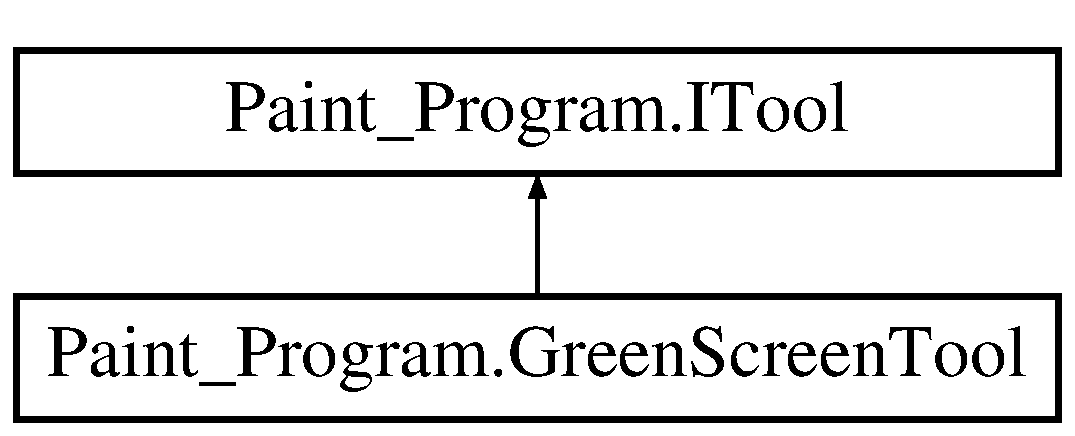
\includegraphics[height=2.000000cm]{class_paint___program_1_1_green_screen_tool}
\end{center}
\end{figure}
\subsection*{Public Member Functions}
\begin{DoxyCompactItemize}
\item 
void \mbox{\hyperlink{class_paint___program_1_1_green_screen_tool_a957c8149c7cc59b1c9734ca5bb5309c7}{Init}} ()
\item 
Bitmap \mbox{\hyperlink{class_paint___program_1_1_green_screen_tool_a883b61f098ace3dc87b8ad92b59fcb6c}{get\+Canvas}} ()
\item 
string \mbox{\hyperlink{class_paint___program_1_1_green_screen_tool_a5d25a6867cc4882d9ec31182829fb24b}{Get\+Tool\+Icon\+Path}} ()
\item 
void \mbox{\hyperlink{class_paint___program_1_1_green_screen_tool_ae3a5e35c0921093957b7cccde92e1b91}{On\+Mouse\+Down}} (object sender, Mouse\+Event\+Args e)
\item 
void \mbox{\hyperlink{class_paint___program_1_1_green_screen_tool_a95699606ba5027c0671f4bc6ef86be93}{On\+Mouse\+Move}} (object sender, Mouse\+Event\+Args e)
\item 
void \mbox{\hyperlink{class_paint___program_1_1_green_screen_tool_ad6be969ae981c34f5677e8a5bd537ef6}{On\+Mouse\+Up}} (object sender, Mouse\+Event\+Args e)
\item 
bool \mbox{\hyperlink{class_paint___program_1_1_green_screen_tool_a94a122c3229b5f530531228837234eb0}{is\+Initalized}} ()
\item 
Bitmap \mbox{\hyperlink{class_paint___program_1_1_green_screen_tool_a02fd2ecf253f8eeb746d1e78eedb08a2}{Get\+Tool\+Layer}} ()
\item 
bool \mbox{\hyperlink{class_paint___program_1_1_green_screen_tool_a554c35de10b5876aa936961177344a59}{Requires\+Layer\+Data}} ()
\item 
void \mbox{\hyperlink{class_paint___program_1_1_green_screen_tool_ad17100eea4bbfc96072cf4525ea053c4}{Set\+Layer\+Data}} (Bitmap bit)
\item 
string \mbox{\hyperlink{class_paint___program_1_1_green_screen_tool_af580394652e180ac8f0acfb79704ffa4}{Get\+Tool\+Tip}} ()
\item 
void \mbox{\hyperlink{class_paint___program_1_1_green_screen_tool_a3d474370bf269af763ff6edceebd2000}{Update\+Interface\+Layer}} ()
\end{DoxyCompactItemize}
\subsection*{Private Member Functions}
\begin{DoxyCompactItemize}
\item 
double \mbox{\hyperlink{class_paint___program_1_1_green_screen_tool_a5da8c478fc4640e8250f1186b2ae8f74}{Distance}} (int x1, int y1, int z1, int x2, int y2, int z2)
\end{DoxyCompactItemize}
\subsection*{Private Attributes}
\begin{DoxyCompactItemize}
\item 
Graphics \mbox{\hyperlink{class_paint___program_1_1_green_screen_tool_aca8f9a5ec0d983848de921e801e8ed7f}{graphics}}
\item 
int \mbox{\hyperlink{class_paint___program_1_1_green_screen_tool_ac6e91de82caa4c468999d4cbc5eca45e}{width}}
\item 
int \mbox{\hyperlink{class_paint___program_1_1_green_screen_tool_a679ac45d198acb71fb2f92e663bbbd2b}{height}}
\item 
bool \mbox{\hyperlink{class_paint___program_1_1_green_screen_tool_a0a46a665af35d9e10a0edb47ff845b19}{b\+Active}}
\item 
bool \mbox{\hyperlink{class_paint___program_1_1_green_screen_tool_a62a6e0d3f19e085a50a08bb1d9b1849d}{b\+Mouse\+Down}}
\item 
bool \mbox{\hyperlink{class_paint___program_1_1_green_screen_tool_a988a8407916d4ad8f1d82e3118886834}{b\+Init}}
\item 
Bitmap \mbox{\hyperlink{class_paint___program_1_1_green_screen_tool_a1bf0fa58eacb1bd8adf711c0f56223d4}{b\+Layer}}
\end{DoxyCompactItemize}


\subsection{Member Function Documentation}
\mbox{\Hypertarget{class_paint___program_1_1_green_screen_tool_a5da8c478fc4640e8250f1186b2ae8f74}\label{class_paint___program_1_1_green_screen_tool_a5da8c478fc4640e8250f1186b2ae8f74}} 
\index{Paint\+\_\+\+Program\+::\+Green\+Screen\+Tool@{Paint\+\_\+\+Program\+::\+Green\+Screen\+Tool}!Distance@{Distance}}
\index{Distance@{Distance}!Paint\+\_\+\+Program\+::\+Green\+Screen\+Tool@{Paint\+\_\+\+Program\+::\+Green\+Screen\+Tool}}
\subsubsection{\texorpdfstring{Distance()}{Distance()}}
{\footnotesize\ttfamily double Paint\+\_\+\+Program.\+Green\+Screen\+Tool.\+Distance (\begin{DoxyParamCaption}\item[{int}]{x1,  }\item[{int}]{y1,  }\item[{int}]{z1,  }\item[{int}]{x2,  }\item[{int}]{y2,  }\item[{int}]{z2 }\end{DoxyParamCaption})\hspace{0.3cm}{\ttfamily [inline]}, {\ttfamily [private]}}

\mbox{\Hypertarget{class_paint___program_1_1_green_screen_tool_a883b61f098ace3dc87b8ad92b59fcb6c}\label{class_paint___program_1_1_green_screen_tool_a883b61f098ace3dc87b8ad92b59fcb6c}} 
\index{Paint\+\_\+\+Program\+::\+Green\+Screen\+Tool@{Paint\+\_\+\+Program\+::\+Green\+Screen\+Tool}!get\+Canvas@{get\+Canvas}}
\index{get\+Canvas@{get\+Canvas}!Paint\+\_\+\+Program\+::\+Green\+Screen\+Tool@{Paint\+\_\+\+Program\+::\+Green\+Screen\+Tool}}
\subsubsection{\texorpdfstring{get\+Canvas()}{getCanvas()}}
{\footnotesize\ttfamily Bitmap Paint\+\_\+\+Program.\+Green\+Screen\+Tool.\+get\+Canvas (\begin{DoxyParamCaption}{ }\end{DoxyParamCaption})\hspace{0.3cm}{\ttfamily [inline]}}

\mbox{\Hypertarget{class_paint___program_1_1_green_screen_tool_a5d25a6867cc4882d9ec31182829fb24b}\label{class_paint___program_1_1_green_screen_tool_a5d25a6867cc4882d9ec31182829fb24b}} 
\index{Paint\+\_\+\+Program\+::\+Green\+Screen\+Tool@{Paint\+\_\+\+Program\+::\+Green\+Screen\+Tool}!Get\+Tool\+Icon\+Path@{Get\+Tool\+Icon\+Path}}
\index{Get\+Tool\+Icon\+Path@{Get\+Tool\+Icon\+Path}!Paint\+\_\+\+Program\+::\+Green\+Screen\+Tool@{Paint\+\_\+\+Program\+::\+Green\+Screen\+Tool}}
\subsubsection{\texorpdfstring{Get\+Tool\+Icon\+Path()}{GetToolIconPath()}}
{\footnotesize\ttfamily string Paint\+\_\+\+Program.\+Green\+Screen\+Tool.\+Get\+Tool\+Icon\+Path (\begin{DoxyParamCaption}{ }\end{DoxyParamCaption})\hspace{0.3cm}{\ttfamily [inline]}}



Implements \mbox{\hyperlink{interface_paint___program_1_1_i_tool_aa057d2f99c59d7bec0215dcad2da1b72}{Paint\+\_\+\+Program.\+I\+Tool}}.

\mbox{\Hypertarget{class_paint___program_1_1_green_screen_tool_a02fd2ecf253f8eeb746d1e78eedb08a2}\label{class_paint___program_1_1_green_screen_tool_a02fd2ecf253f8eeb746d1e78eedb08a2}} 
\index{Paint\+\_\+\+Program\+::\+Green\+Screen\+Tool@{Paint\+\_\+\+Program\+::\+Green\+Screen\+Tool}!Get\+Tool\+Layer@{Get\+Tool\+Layer}}
\index{Get\+Tool\+Layer@{Get\+Tool\+Layer}!Paint\+\_\+\+Program\+::\+Green\+Screen\+Tool@{Paint\+\_\+\+Program\+::\+Green\+Screen\+Tool}}
\subsubsection{\texorpdfstring{Get\+Tool\+Layer()}{GetToolLayer()}}
{\footnotesize\ttfamily Bitmap Paint\+\_\+\+Program.\+Green\+Screen\+Tool.\+Get\+Tool\+Layer (\begin{DoxyParamCaption}{ }\end{DoxyParamCaption})\hspace{0.3cm}{\ttfamily [inline]}}



Implements \mbox{\hyperlink{interface_paint___program_1_1_i_tool_a9b057905515f42a988c166a6a40318e0}{Paint\+\_\+\+Program.\+I\+Tool}}.

\mbox{\Hypertarget{class_paint___program_1_1_green_screen_tool_af580394652e180ac8f0acfb79704ffa4}\label{class_paint___program_1_1_green_screen_tool_af580394652e180ac8f0acfb79704ffa4}} 
\index{Paint\+\_\+\+Program\+::\+Green\+Screen\+Tool@{Paint\+\_\+\+Program\+::\+Green\+Screen\+Tool}!Get\+Tool\+Tip@{Get\+Tool\+Tip}}
\index{Get\+Tool\+Tip@{Get\+Tool\+Tip}!Paint\+\_\+\+Program\+::\+Green\+Screen\+Tool@{Paint\+\_\+\+Program\+::\+Green\+Screen\+Tool}}
\subsubsection{\texorpdfstring{Get\+Tool\+Tip()}{GetToolTip()}}
{\footnotesize\ttfamily string Paint\+\_\+\+Program.\+Green\+Screen\+Tool.\+Get\+Tool\+Tip (\begin{DoxyParamCaption}{ }\end{DoxyParamCaption})\hspace{0.3cm}{\ttfamily [inline]}}



Implements \mbox{\hyperlink{interface_paint___program_1_1_i_tool_ac11f1591587144b6e74f5767bbf1df56}{Paint\+\_\+\+Program.\+I\+Tool}}.

\mbox{\Hypertarget{class_paint___program_1_1_green_screen_tool_a957c8149c7cc59b1c9734ca5bb5309c7}\label{class_paint___program_1_1_green_screen_tool_a957c8149c7cc59b1c9734ca5bb5309c7}} 
\index{Paint\+\_\+\+Program\+::\+Green\+Screen\+Tool@{Paint\+\_\+\+Program\+::\+Green\+Screen\+Tool}!Init@{Init}}
\index{Init@{Init}!Paint\+\_\+\+Program\+::\+Green\+Screen\+Tool@{Paint\+\_\+\+Program\+::\+Green\+Screen\+Tool}}
\subsubsection{\texorpdfstring{Init()}{Init()}}
{\footnotesize\ttfamily void Paint\+\_\+\+Program.\+Green\+Screen\+Tool.\+Init (\begin{DoxyParamCaption}{ }\end{DoxyParamCaption})\hspace{0.3cm}{\ttfamily [inline]}}



Implements \mbox{\hyperlink{interface_paint___program_1_1_i_tool_af823123a30fbda34e24e907243241046}{Paint\+\_\+\+Program.\+I\+Tool}}.

\mbox{\Hypertarget{class_paint___program_1_1_green_screen_tool_a94a122c3229b5f530531228837234eb0}\label{class_paint___program_1_1_green_screen_tool_a94a122c3229b5f530531228837234eb0}} 
\index{Paint\+\_\+\+Program\+::\+Green\+Screen\+Tool@{Paint\+\_\+\+Program\+::\+Green\+Screen\+Tool}!is\+Initalized@{is\+Initalized}}
\index{is\+Initalized@{is\+Initalized}!Paint\+\_\+\+Program\+::\+Green\+Screen\+Tool@{Paint\+\_\+\+Program\+::\+Green\+Screen\+Tool}}
\subsubsection{\texorpdfstring{is\+Initalized()}{isInitalized()}}
{\footnotesize\ttfamily bool Paint\+\_\+\+Program.\+Green\+Screen\+Tool.\+is\+Initalized (\begin{DoxyParamCaption}{ }\end{DoxyParamCaption})\hspace{0.3cm}{\ttfamily [inline]}}



Implements \mbox{\hyperlink{interface_paint___program_1_1_i_tool_a951b844bcbf47a6c306104fa86be7a5d}{Paint\+\_\+\+Program.\+I\+Tool}}.

\mbox{\Hypertarget{class_paint___program_1_1_green_screen_tool_ae3a5e35c0921093957b7cccde92e1b91}\label{class_paint___program_1_1_green_screen_tool_ae3a5e35c0921093957b7cccde92e1b91}} 
\index{Paint\+\_\+\+Program\+::\+Green\+Screen\+Tool@{Paint\+\_\+\+Program\+::\+Green\+Screen\+Tool}!On\+Mouse\+Down@{On\+Mouse\+Down}}
\index{On\+Mouse\+Down@{On\+Mouse\+Down}!Paint\+\_\+\+Program\+::\+Green\+Screen\+Tool@{Paint\+\_\+\+Program\+::\+Green\+Screen\+Tool}}
\subsubsection{\texorpdfstring{On\+Mouse\+Down()}{OnMouseDown()}}
{\footnotesize\ttfamily void Paint\+\_\+\+Program.\+Green\+Screen\+Tool.\+On\+Mouse\+Down (\begin{DoxyParamCaption}\item[{object}]{sender,  }\item[{Mouse\+Event\+Args}]{e }\end{DoxyParamCaption})\hspace{0.3cm}{\ttfamily [inline]}}



Implements \mbox{\hyperlink{interface_paint___program_1_1_i_tool_a73d8797f4f2b1e0d8efe8aadcd44e840}{Paint\+\_\+\+Program.\+I\+Tool}}.

\mbox{\Hypertarget{class_paint___program_1_1_green_screen_tool_a95699606ba5027c0671f4bc6ef86be93}\label{class_paint___program_1_1_green_screen_tool_a95699606ba5027c0671f4bc6ef86be93}} 
\index{Paint\+\_\+\+Program\+::\+Green\+Screen\+Tool@{Paint\+\_\+\+Program\+::\+Green\+Screen\+Tool}!On\+Mouse\+Move@{On\+Mouse\+Move}}
\index{On\+Mouse\+Move@{On\+Mouse\+Move}!Paint\+\_\+\+Program\+::\+Green\+Screen\+Tool@{Paint\+\_\+\+Program\+::\+Green\+Screen\+Tool}}
\subsubsection{\texorpdfstring{On\+Mouse\+Move()}{OnMouseMove()}}
{\footnotesize\ttfamily void Paint\+\_\+\+Program.\+Green\+Screen\+Tool.\+On\+Mouse\+Move (\begin{DoxyParamCaption}\item[{object}]{sender,  }\item[{Mouse\+Event\+Args}]{e }\end{DoxyParamCaption})\hspace{0.3cm}{\ttfamily [inline]}}



Implements \mbox{\hyperlink{interface_paint___program_1_1_i_tool_a6a1cbe840b5cfc8a9b9463cc21590845}{Paint\+\_\+\+Program.\+I\+Tool}}.

\mbox{\Hypertarget{class_paint___program_1_1_green_screen_tool_ad6be969ae981c34f5677e8a5bd537ef6}\label{class_paint___program_1_1_green_screen_tool_ad6be969ae981c34f5677e8a5bd537ef6}} 
\index{Paint\+\_\+\+Program\+::\+Green\+Screen\+Tool@{Paint\+\_\+\+Program\+::\+Green\+Screen\+Tool}!On\+Mouse\+Up@{On\+Mouse\+Up}}
\index{On\+Mouse\+Up@{On\+Mouse\+Up}!Paint\+\_\+\+Program\+::\+Green\+Screen\+Tool@{Paint\+\_\+\+Program\+::\+Green\+Screen\+Tool}}
\subsubsection{\texorpdfstring{On\+Mouse\+Up()}{OnMouseUp()}}
{\footnotesize\ttfamily void Paint\+\_\+\+Program.\+Green\+Screen\+Tool.\+On\+Mouse\+Up (\begin{DoxyParamCaption}\item[{object}]{sender,  }\item[{Mouse\+Event\+Args}]{e }\end{DoxyParamCaption})\hspace{0.3cm}{\ttfamily [inline]}}



Implements \mbox{\hyperlink{interface_paint___program_1_1_i_tool_a47984c2879213022f1684c07f7bba73e}{Paint\+\_\+\+Program.\+I\+Tool}}.

\mbox{\Hypertarget{class_paint___program_1_1_green_screen_tool_a554c35de10b5876aa936961177344a59}\label{class_paint___program_1_1_green_screen_tool_a554c35de10b5876aa936961177344a59}} 
\index{Paint\+\_\+\+Program\+::\+Green\+Screen\+Tool@{Paint\+\_\+\+Program\+::\+Green\+Screen\+Tool}!Requires\+Layer\+Data@{Requires\+Layer\+Data}}
\index{Requires\+Layer\+Data@{Requires\+Layer\+Data}!Paint\+\_\+\+Program\+::\+Green\+Screen\+Tool@{Paint\+\_\+\+Program\+::\+Green\+Screen\+Tool}}
\subsubsection{\texorpdfstring{Requires\+Layer\+Data()}{RequiresLayerData()}}
{\footnotesize\ttfamily bool Paint\+\_\+\+Program.\+Green\+Screen\+Tool.\+Requires\+Layer\+Data (\begin{DoxyParamCaption}{ }\end{DoxyParamCaption})\hspace{0.3cm}{\ttfamily [inline]}}



Implements \mbox{\hyperlink{interface_paint___program_1_1_i_tool_a6d45b6c48da8130ae41db3a66cdaef9a}{Paint\+\_\+\+Program.\+I\+Tool}}.

\mbox{\Hypertarget{class_paint___program_1_1_green_screen_tool_ad17100eea4bbfc96072cf4525ea053c4}\label{class_paint___program_1_1_green_screen_tool_ad17100eea4bbfc96072cf4525ea053c4}} 
\index{Paint\+\_\+\+Program\+::\+Green\+Screen\+Tool@{Paint\+\_\+\+Program\+::\+Green\+Screen\+Tool}!Set\+Layer\+Data@{Set\+Layer\+Data}}
\index{Set\+Layer\+Data@{Set\+Layer\+Data}!Paint\+\_\+\+Program\+::\+Green\+Screen\+Tool@{Paint\+\_\+\+Program\+::\+Green\+Screen\+Tool}}
\subsubsection{\texorpdfstring{Set\+Layer\+Data()}{SetLayerData()}}
{\footnotesize\ttfamily void Paint\+\_\+\+Program.\+Green\+Screen\+Tool.\+Set\+Layer\+Data (\begin{DoxyParamCaption}\item[{Bitmap}]{bit }\end{DoxyParamCaption})\hspace{0.3cm}{\ttfamily [inline]}}



Implements \mbox{\hyperlink{interface_paint___program_1_1_i_tool_a2d3e63715dfe04075d27dacf367d1633}{Paint\+\_\+\+Program.\+I\+Tool}}.

\mbox{\Hypertarget{class_paint___program_1_1_green_screen_tool_a3d474370bf269af763ff6edceebd2000}\label{class_paint___program_1_1_green_screen_tool_a3d474370bf269af763ff6edceebd2000}} 
\index{Paint\+\_\+\+Program\+::\+Green\+Screen\+Tool@{Paint\+\_\+\+Program\+::\+Green\+Screen\+Tool}!Update\+Interface\+Layer@{Update\+Interface\+Layer}}
\index{Update\+Interface\+Layer@{Update\+Interface\+Layer}!Paint\+\_\+\+Program\+::\+Green\+Screen\+Tool@{Paint\+\_\+\+Program\+::\+Green\+Screen\+Tool}}
\subsubsection{\texorpdfstring{Update\+Interface\+Layer()}{UpdateInterfaceLayer()}}
{\footnotesize\ttfamily void Paint\+\_\+\+Program.\+Green\+Screen\+Tool.\+Update\+Interface\+Layer (\begin{DoxyParamCaption}{ }\end{DoxyParamCaption})\hspace{0.3cm}{\ttfamily [inline]}}



Implements \mbox{\hyperlink{interface_paint___program_1_1_i_tool_a36db75d29e88dfd739f658633c40e955}{Paint\+\_\+\+Program.\+I\+Tool}}.



\subsection{Member Data Documentation}
\mbox{\Hypertarget{class_paint___program_1_1_green_screen_tool_a0a46a665af35d9e10a0edb47ff845b19}\label{class_paint___program_1_1_green_screen_tool_a0a46a665af35d9e10a0edb47ff845b19}} 
\index{Paint\+\_\+\+Program\+::\+Green\+Screen\+Tool@{Paint\+\_\+\+Program\+::\+Green\+Screen\+Tool}!b\+Active@{b\+Active}}
\index{b\+Active@{b\+Active}!Paint\+\_\+\+Program\+::\+Green\+Screen\+Tool@{Paint\+\_\+\+Program\+::\+Green\+Screen\+Tool}}
\subsubsection{\texorpdfstring{b\+Active}{bActive}}
{\footnotesize\ttfamily bool Paint\+\_\+\+Program.\+Green\+Screen\+Tool.\+b\+Active\hspace{0.3cm}{\ttfamily [private]}}

\mbox{\Hypertarget{class_paint___program_1_1_green_screen_tool_a988a8407916d4ad8f1d82e3118886834}\label{class_paint___program_1_1_green_screen_tool_a988a8407916d4ad8f1d82e3118886834}} 
\index{Paint\+\_\+\+Program\+::\+Green\+Screen\+Tool@{Paint\+\_\+\+Program\+::\+Green\+Screen\+Tool}!b\+Init@{b\+Init}}
\index{b\+Init@{b\+Init}!Paint\+\_\+\+Program\+::\+Green\+Screen\+Tool@{Paint\+\_\+\+Program\+::\+Green\+Screen\+Tool}}
\subsubsection{\texorpdfstring{b\+Init}{bInit}}
{\footnotesize\ttfamily bool Paint\+\_\+\+Program.\+Green\+Screen\+Tool.\+b\+Init\hspace{0.3cm}{\ttfamily [private]}}

\mbox{\Hypertarget{class_paint___program_1_1_green_screen_tool_a1bf0fa58eacb1bd8adf711c0f56223d4}\label{class_paint___program_1_1_green_screen_tool_a1bf0fa58eacb1bd8adf711c0f56223d4}} 
\index{Paint\+\_\+\+Program\+::\+Green\+Screen\+Tool@{Paint\+\_\+\+Program\+::\+Green\+Screen\+Tool}!b\+Layer@{b\+Layer}}
\index{b\+Layer@{b\+Layer}!Paint\+\_\+\+Program\+::\+Green\+Screen\+Tool@{Paint\+\_\+\+Program\+::\+Green\+Screen\+Tool}}
\subsubsection{\texorpdfstring{b\+Layer}{bLayer}}
{\footnotesize\ttfamily Bitmap Paint\+\_\+\+Program.\+Green\+Screen\+Tool.\+b\+Layer\hspace{0.3cm}{\ttfamily [private]}}

\mbox{\Hypertarget{class_paint___program_1_1_green_screen_tool_a62a6e0d3f19e085a50a08bb1d9b1849d}\label{class_paint___program_1_1_green_screen_tool_a62a6e0d3f19e085a50a08bb1d9b1849d}} 
\index{Paint\+\_\+\+Program\+::\+Green\+Screen\+Tool@{Paint\+\_\+\+Program\+::\+Green\+Screen\+Tool}!b\+Mouse\+Down@{b\+Mouse\+Down}}
\index{b\+Mouse\+Down@{b\+Mouse\+Down}!Paint\+\_\+\+Program\+::\+Green\+Screen\+Tool@{Paint\+\_\+\+Program\+::\+Green\+Screen\+Tool}}
\subsubsection{\texorpdfstring{b\+Mouse\+Down}{bMouseDown}}
{\footnotesize\ttfamily bool Paint\+\_\+\+Program.\+Green\+Screen\+Tool.\+b\+Mouse\+Down\hspace{0.3cm}{\ttfamily [private]}}

\mbox{\Hypertarget{class_paint___program_1_1_green_screen_tool_aca8f9a5ec0d983848de921e801e8ed7f}\label{class_paint___program_1_1_green_screen_tool_aca8f9a5ec0d983848de921e801e8ed7f}} 
\index{Paint\+\_\+\+Program\+::\+Green\+Screen\+Tool@{Paint\+\_\+\+Program\+::\+Green\+Screen\+Tool}!graphics@{graphics}}
\index{graphics@{graphics}!Paint\+\_\+\+Program\+::\+Green\+Screen\+Tool@{Paint\+\_\+\+Program\+::\+Green\+Screen\+Tool}}
\subsubsection{\texorpdfstring{graphics}{graphics}}
{\footnotesize\ttfamily Graphics Paint\+\_\+\+Program.\+Green\+Screen\+Tool.\+graphics\hspace{0.3cm}{\ttfamily [private]}}

\mbox{\Hypertarget{class_paint___program_1_1_green_screen_tool_a679ac45d198acb71fb2f92e663bbbd2b}\label{class_paint___program_1_1_green_screen_tool_a679ac45d198acb71fb2f92e663bbbd2b}} 
\index{Paint\+\_\+\+Program\+::\+Green\+Screen\+Tool@{Paint\+\_\+\+Program\+::\+Green\+Screen\+Tool}!height@{height}}
\index{height@{height}!Paint\+\_\+\+Program\+::\+Green\+Screen\+Tool@{Paint\+\_\+\+Program\+::\+Green\+Screen\+Tool}}
\subsubsection{\texorpdfstring{height}{height}}
{\footnotesize\ttfamily int Paint\+\_\+\+Program.\+Green\+Screen\+Tool.\+height\hspace{0.3cm}{\ttfamily [private]}}

\mbox{\Hypertarget{class_paint___program_1_1_green_screen_tool_ac6e91de82caa4c468999d4cbc5eca45e}\label{class_paint___program_1_1_green_screen_tool_ac6e91de82caa4c468999d4cbc5eca45e}} 
\index{Paint\+\_\+\+Program\+::\+Green\+Screen\+Tool@{Paint\+\_\+\+Program\+::\+Green\+Screen\+Tool}!width@{width}}
\index{width@{width}!Paint\+\_\+\+Program\+::\+Green\+Screen\+Tool@{Paint\+\_\+\+Program\+::\+Green\+Screen\+Tool}}
\subsubsection{\texorpdfstring{width}{width}}
{\footnotesize\ttfamily int Paint\+\_\+\+Program.\+Green\+Screen\+Tool.\+width\hspace{0.3cm}{\ttfamily [private]}}



The documentation for this class was generated from the following file\+:\begin{DoxyCompactItemize}
\item 
Paint Program/\mbox{\hyperlink{_green_screen_tool_8cs}{Green\+Screen\+Tool.\+cs}}\end{DoxyCompactItemize}

\hypertarget{class_wintab_d_n_1_1_h_c_t_x}{}\section{Wintab\+D\+N.\+H\+C\+TX Class Reference}
\label{class_wintab_d_n_1_1_h_c_t_x}\index{Wintab\+D\+N.\+H\+C\+TX@{Wintab\+D\+N.\+H\+C\+TX}}


Managed implementation of Wintab \mbox{\hyperlink{class_wintab_d_n_1_1_h_c_t_x}{H\+C\+TX}} typedef. Holds a Wintab context identifier.  




\subsection{Detailed Description}
Managed implementation of Wintab \mbox{\hyperlink{class_wintab_d_n_1_1_h_c_t_x}{H\+C\+TX}} typedef. Holds a Wintab context identifier. 



The documentation for this class was generated from the following file\+:\begin{DoxyCompactItemize}
\item 
Wintab\+D\+N/\mbox{\hyperlink{_c_wintab_funcs_8cs}{C\+Wintab\+Funcs.\+cs}}\end{DoxyCompactItemize}

\hypertarget{struct_wintab_d_n_1_1_h_w_n_d}{}\section{Wintab\+D\+N.\+H\+W\+ND Struct Reference}
\label{struct_wintab_d_n_1_1_h_w_n_d}\index{Wintab\+D\+N.\+H\+W\+ND@{Wintab\+D\+N.\+H\+W\+ND}}


Managed implementation of Wintab \mbox{\hyperlink{struct_wintab_d_n_1_1_h_w_n_d}{H\+W\+ND}} typedef. Holds native Window handle.  




\subsection{Detailed Description}
Managed implementation of Wintab \mbox{\hyperlink{struct_wintab_d_n_1_1_h_w_n_d}{H\+W\+ND}} typedef. Holds native Window handle. 



The documentation for this struct was generated from the following file\+:\begin{DoxyCompactItemize}
\item 
Wintab\+D\+N/\mbox{\hyperlink{_c_wintab_funcs_8cs}{C\+Wintab\+Funcs.\+cs}}\end{DoxyCompactItemize}

\hypertarget{class_paint___program_1_1_image_import}{}\section{Paint\+\_\+\+Program.\+Image\+Import Class Reference}
\label{class_paint___program_1_1_image_import}\index{Paint\+\_\+\+Program.\+Image\+Import@{Paint\+\_\+\+Program.\+Image\+Import}}
\subsection*{Public Member Functions}
\begin{DoxyCompactItemize}
\item 
\mbox{\hyperlink{class_paint___program_1_1_image_import_a5765b2ce24cc009c2a15398af17a977a}{Image\+Import}} ()
\end{DoxyCompactItemize}
\subsection*{Private Member Functions}
\begin{DoxyCompactItemize}
\item 
void \mbox{\hyperlink{class_paint___program_1_1_image_import_ae00dcd97307687b44917c11645487a1a}{do\+Open}} (Open\+File\+Dialog ofd, object sender, Do\+Work\+Event\+Args args)
\end{DoxyCompactItemize}


\subsection{Constructor \& Destructor Documentation}
\mbox{\Hypertarget{class_paint___program_1_1_image_import_a5765b2ce24cc009c2a15398af17a977a}\label{class_paint___program_1_1_image_import_a5765b2ce24cc009c2a15398af17a977a}} 
\index{Paint\+\_\+\+Program\+::\+Image\+Import@{Paint\+\_\+\+Program\+::\+Image\+Import}!Image\+Import@{Image\+Import}}
\index{Image\+Import@{Image\+Import}!Paint\+\_\+\+Program\+::\+Image\+Import@{Paint\+\_\+\+Program\+::\+Image\+Import}}
\subsubsection{\texorpdfstring{Image\+Import()}{ImageImport()}}
{\footnotesize\ttfamily Paint\+\_\+\+Program.\+Image\+Import.\+Image\+Import (\begin{DoxyParamCaption}{ }\end{DoxyParamCaption})\hspace{0.3cm}{\ttfamily [inline]}}



\subsection{Member Function Documentation}
\mbox{\Hypertarget{class_paint___program_1_1_image_import_ae00dcd97307687b44917c11645487a1a}\label{class_paint___program_1_1_image_import_ae00dcd97307687b44917c11645487a1a}} 
\index{Paint\+\_\+\+Program\+::\+Image\+Import@{Paint\+\_\+\+Program\+::\+Image\+Import}!do\+Open@{do\+Open}}
\index{do\+Open@{do\+Open}!Paint\+\_\+\+Program\+::\+Image\+Import@{Paint\+\_\+\+Program\+::\+Image\+Import}}
\subsubsection{\texorpdfstring{do\+Open()}{doOpen()}}
{\footnotesize\ttfamily void Paint\+\_\+\+Program.\+Image\+Import.\+do\+Open (\begin{DoxyParamCaption}\item[{Open\+File\+Dialog}]{ofd,  }\item[{object}]{sender,  }\item[{Do\+Work\+Event\+Args}]{args }\end{DoxyParamCaption})\hspace{0.3cm}{\ttfamily [inline]}, {\ttfamily [private]}}



The documentation for this class was generated from the following file\+:\begin{DoxyCompactItemize}
\item 
Paint Program/\mbox{\hyperlink{_image_import_8cs}{Image\+Import.\+cs}}\end{DoxyCompactItemize}

\hypertarget{interface_paint___program_1_1_i_text_update}{}\section{Paint\+\_\+\+Program.\+I\+Text\+Update Interface Reference}
\label{interface_paint___program_1_1_i_text_update}\index{Paint\+\_\+\+Program.\+I\+Text\+Update@{Paint\+\_\+\+Program.\+I\+Text\+Update}}
Inheritance diagram for Paint\+\_\+\+Program.\+I\+Text\+Update\+:\begin{figure}[H]
\begin{center}
\leavevmode
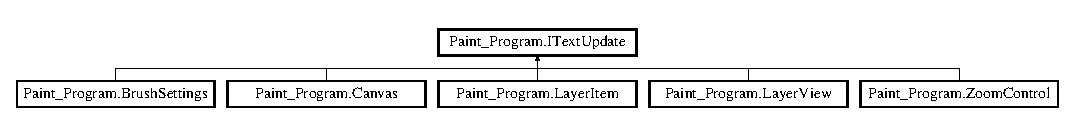
\includegraphics[height=1.217391cm]{interface_paint___program_1_1_i_text_update}
\end{center}
\end{figure}
\subsection*{Public Member Functions}
\begin{DoxyCompactItemize}
\item 
void \mbox{\hyperlink{interface_paint___program_1_1_i_text_update_ad1e94db137571608917117e9a6f7479b}{Update\+Text}} ()
\end{DoxyCompactItemize}


\subsection{Member Function Documentation}
\mbox{\Hypertarget{interface_paint___program_1_1_i_text_update_ad1e94db137571608917117e9a6f7479b}\label{interface_paint___program_1_1_i_text_update_ad1e94db137571608917117e9a6f7479b}} 
\index{Paint\+\_\+\+Program\+::\+I\+Text\+Update@{Paint\+\_\+\+Program\+::\+I\+Text\+Update}!Update\+Text@{Update\+Text}}
\index{Update\+Text@{Update\+Text}!Paint\+\_\+\+Program\+::\+I\+Text\+Update@{Paint\+\_\+\+Program\+::\+I\+Text\+Update}}
\subsubsection{\texorpdfstring{Update\+Text()}{UpdateText()}}
{\footnotesize\ttfamily void Paint\+\_\+\+Program.\+I\+Text\+Update.\+Update\+Text (\begin{DoxyParamCaption}{ }\end{DoxyParamCaption})}



Implemented in \mbox{\hyperlink{class_paint___program_1_1_canvas_ad80b3ef48814a229e01a330b49344f3b}{Paint\+\_\+\+Program.\+Canvas}}, \mbox{\hyperlink{class_paint___program_1_1_layer_view_a9524e183d6c00b15c217e9d5c1d14aea}{Paint\+\_\+\+Program.\+Layer\+View}}, \mbox{\hyperlink{class_paint___program_1_1_layer_item_a7cbff967883c3895e000050a5c6e2144}{Paint\+\_\+\+Program.\+Layer\+Item}}, \mbox{\hyperlink{class_paint___program_1_1_zoom_control_ab67ee2f3ff5a99c50279ac3b3602a523}{Paint\+\_\+\+Program.\+Zoom\+Control}}, and \mbox{\hyperlink{class_paint___program_1_1_brush_settings_a0669e5f09b62b9545e408f39689f30ed}{Paint\+\_\+\+Program.\+Brush\+Settings}}.



The documentation for this interface was generated from the following file\+:\begin{DoxyCompactItemize}
\item 
Paint Program/\mbox{\hyperlink{_i_text_update_8cs}{I\+Text\+Update.\+cs}}\end{DoxyCompactItemize}

\hypertarget{interface_paint___program_1_1_i_tool}{}\section{Paint\+\_\+\+Program.\+I\+Tool Interface Reference}
\label{interface_paint___program_1_1_i_tool}\index{Paint\+\_\+\+Program.\+I\+Tool@{Paint\+\_\+\+Program.\+I\+Tool}}
Inheritance diagram for Paint\+\_\+\+Program.\+I\+Tool\+:\begin{figure}[H]
\begin{center}
\leavevmode
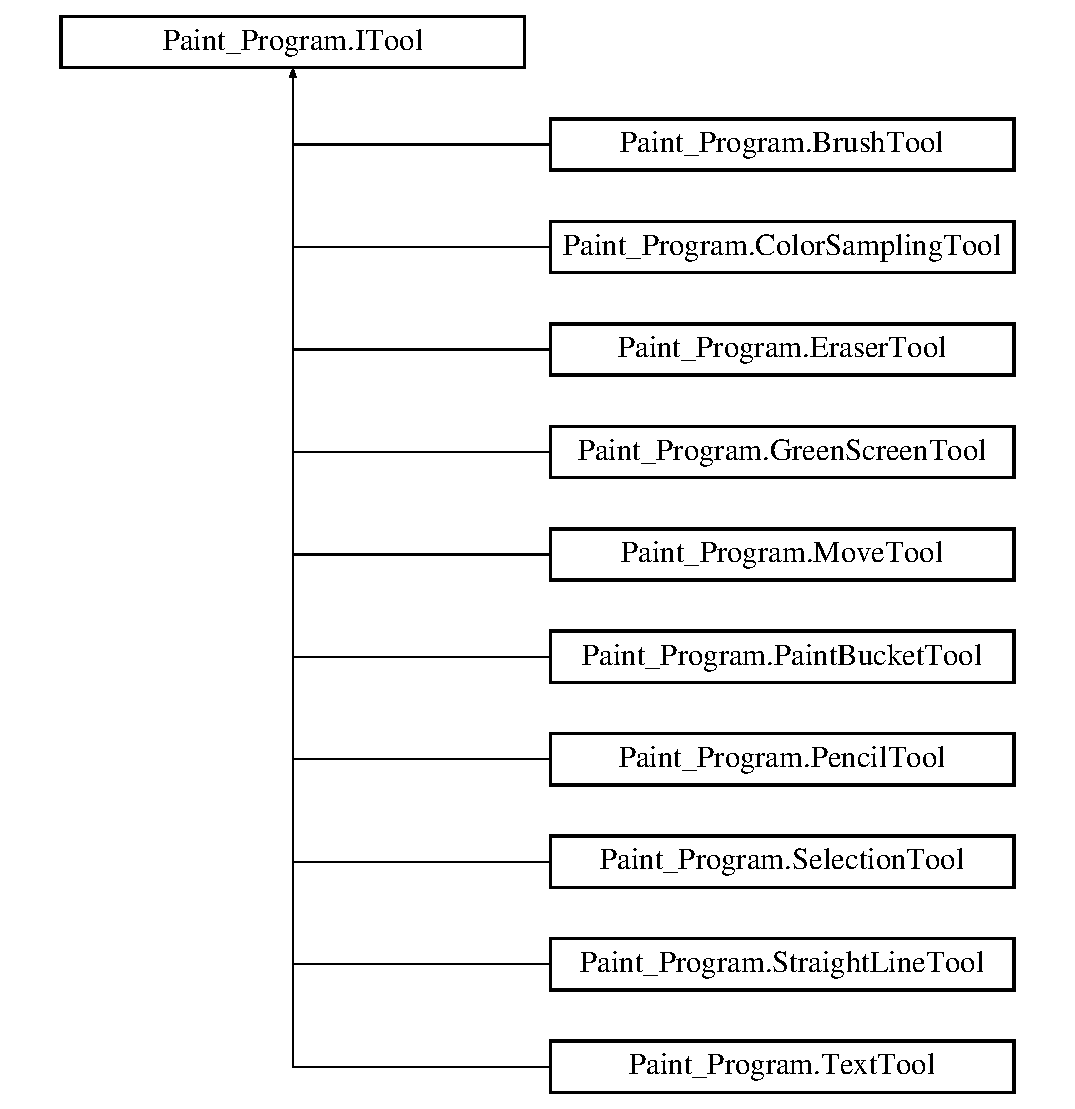
\includegraphics[height=11.000000cm]{interface_paint___program_1_1_i_tool}
\end{center}
\end{figure}
\subsection*{Public Member Functions}
\begin{DoxyCompactItemize}
\item 
void \mbox{\hyperlink{interface_paint___program_1_1_i_tool_af823123a30fbda34e24e907243241046}{Init}} ()
\item 
Bitmap \mbox{\hyperlink{interface_paint___program_1_1_i_tool_a9b057905515f42a988c166a6a40318e0}{Get\+Tool\+Layer}} ()
\item 
void \mbox{\hyperlink{interface_paint___program_1_1_i_tool_a73d8797f4f2b1e0d8efe8aadcd44e840}{On\+Mouse\+Down}} (object sender, Mouse\+Event\+Args e)
\item 
void \mbox{\hyperlink{interface_paint___program_1_1_i_tool_a47984c2879213022f1684c07f7bba73e}{On\+Mouse\+Up}} (object sender, Mouse\+Event\+Args e)
\item 
void \mbox{\hyperlink{interface_paint___program_1_1_i_tool_a6a1cbe840b5cfc8a9b9463cc21590845}{On\+Mouse\+Move}} (object sender, Mouse\+Event\+Args e)
\item 
bool \mbox{\hyperlink{interface_paint___program_1_1_i_tool_a951b844bcbf47a6c306104fa86be7a5d}{is\+Initalized}} ()
\item 
string \mbox{\hyperlink{interface_paint___program_1_1_i_tool_aa057d2f99c59d7bec0215dcad2da1b72}{Get\+Tool\+Icon\+Path}} ()
\item 
string \mbox{\hyperlink{interface_paint___program_1_1_i_tool_ac11f1591587144b6e74f5767bbf1df56}{Get\+Tool\+Tip}} ()
\item 
bool \mbox{\hyperlink{interface_paint___program_1_1_i_tool_a6d45b6c48da8130ae41db3a66cdaef9a}{Requires\+Layer\+Data}} ()
\item 
void \mbox{\hyperlink{interface_paint___program_1_1_i_tool_a2d3e63715dfe04075d27dacf367d1633}{Set\+Layer\+Data}} (Bitmap bit)
\item 
void \mbox{\hyperlink{interface_paint___program_1_1_i_tool_a36db75d29e88dfd739f658633c40e955}{Update\+Interface\+Layer}} ()
\end{DoxyCompactItemize}


\subsection{Member Function Documentation}
\mbox{\Hypertarget{interface_paint___program_1_1_i_tool_aa057d2f99c59d7bec0215dcad2da1b72}\label{interface_paint___program_1_1_i_tool_aa057d2f99c59d7bec0215dcad2da1b72}} 
\index{Paint\+\_\+\+Program\+::\+I\+Tool@{Paint\+\_\+\+Program\+::\+I\+Tool}!Get\+Tool\+Icon\+Path@{Get\+Tool\+Icon\+Path}}
\index{Get\+Tool\+Icon\+Path@{Get\+Tool\+Icon\+Path}!Paint\+\_\+\+Program\+::\+I\+Tool@{Paint\+\_\+\+Program\+::\+I\+Tool}}
\subsubsection{\texorpdfstring{Get\+Tool\+Icon\+Path()}{GetToolIconPath()}}
{\footnotesize\ttfamily string Paint\+\_\+\+Program.\+I\+Tool.\+Get\+Tool\+Icon\+Path (\begin{DoxyParamCaption}{ }\end{DoxyParamCaption})}



Implemented in \mbox{\hyperlink{class_paint___program_1_1_brush_tool_a7cc103269b01a6367edce7c994443739}{Paint\+\_\+\+Program.\+Brush\+Tool}}, \mbox{\hyperlink{class_paint___program_1_1_straight_line_tool_ae260a0f50ea86b9ae9cceb36d1093057}{Paint\+\_\+\+Program.\+Straight\+Line\+Tool}}, \mbox{\hyperlink{class_paint___program_1_1_paint_bucket_tool_aef69a21dec547869dde171a604bf1492}{Paint\+\_\+\+Program.\+Paint\+Bucket\+Tool}}, \mbox{\hyperlink{class_paint___program_1_1_text_tool_a0adfe4c942f7d97c2d9cf626fb3b78c7}{Paint\+\_\+\+Program.\+Text\+Tool}}, \mbox{\hyperlink{class_paint___program_1_1_pencil_tool_a91c7f9e9bd173b3f859cbc37f44c4f48}{Paint\+\_\+\+Program.\+Pencil\+Tool}}, \mbox{\hyperlink{class_paint___program_1_1_color_sampling_tool_a319d9e67417e473d0f76b8cafc1d7c2b}{Paint\+\_\+\+Program.\+Color\+Sampling\+Tool}}, \mbox{\hyperlink{class_paint___program_1_1_green_screen_tool_a5d25a6867cc4882d9ec31182829fb24b}{Paint\+\_\+\+Program.\+Green\+Screen\+Tool}}, \mbox{\hyperlink{class_paint___program_1_1_move_tool_a6341409c4de402ff447db2c542cc6b5b}{Paint\+\_\+\+Program.\+Move\+Tool}}, \mbox{\hyperlink{class_paint___program_1_1_eraser_tool_a5a1cb5d84a01983064c68a8dc6023ae6}{Paint\+\_\+\+Program.\+Eraser\+Tool}}, and \mbox{\hyperlink{class_paint___program_1_1_selection_tool_ac93f281cfcc677551b140c350661d9df}{Paint\+\_\+\+Program.\+Selection\+Tool}}.

\mbox{\Hypertarget{interface_paint___program_1_1_i_tool_a9b057905515f42a988c166a6a40318e0}\label{interface_paint___program_1_1_i_tool_a9b057905515f42a988c166a6a40318e0}} 
\index{Paint\+\_\+\+Program\+::\+I\+Tool@{Paint\+\_\+\+Program\+::\+I\+Tool}!Get\+Tool\+Layer@{Get\+Tool\+Layer}}
\index{Get\+Tool\+Layer@{Get\+Tool\+Layer}!Paint\+\_\+\+Program\+::\+I\+Tool@{Paint\+\_\+\+Program\+::\+I\+Tool}}
\subsubsection{\texorpdfstring{Get\+Tool\+Layer()}{GetToolLayer()}}
{\footnotesize\ttfamily Bitmap Paint\+\_\+\+Program.\+I\+Tool.\+Get\+Tool\+Layer (\begin{DoxyParamCaption}{ }\end{DoxyParamCaption})}



Implemented in \mbox{\hyperlink{class_paint___program_1_1_paint_bucket_tool_a3167ad9df7812f1f857e0a869a455ff6}{Paint\+\_\+\+Program.\+Paint\+Bucket\+Tool}}, \mbox{\hyperlink{class_paint___program_1_1_brush_tool_ae96d4b9560f8d271694abd1e727dd14c}{Paint\+\_\+\+Program.\+Brush\+Tool}}, \mbox{\hyperlink{class_paint___program_1_1_straight_line_tool_adb914fa4551bfee82d074838032d030b}{Paint\+\_\+\+Program.\+Straight\+Line\+Tool}}, \mbox{\hyperlink{class_paint___program_1_1_pencil_tool_acef50de4028855c4a6be1ff9f63f9b3b}{Paint\+\_\+\+Program.\+Pencil\+Tool}}, \mbox{\hyperlink{class_paint___program_1_1_green_screen_tool_a02fd2ecf253f8eeb746d1e78eedb08a2}{Paint\+\_\+\+Program.\+Green\+Screen\+Tool}}, \mbox{\hyperlink{class_paint___program_1_1_text_tool_acb2114b449f982664f1fd49e3bb0b017}{Paint\+\_\+\+Program.\+Text\+Tool}}, \mbox{\hyperlink{class_paint___program_1_1_eraser_tool_a2ba0d80771829d2410b5d9a26a6896b2}{Paint\+\_\+\+Program.\+Eraser\+Tool}}, \mbox{\hyperlink{class_paint___program_1_1_color_sampling_tool_aa0e2ac4d50f9a46c0d83a226e9e701c8}{Paint\+\_\+\+Program.\+Color\+Sampling\+Tool}}, \mbox{\hyperlink{class_paint___program_1_1_move_tool_a1d458ccea18d91c95d7da179fc3503e2}{Paint\+\_\+\+Program.\+Move\+Tool}}, and \mbox{\hyperlink{class_paint___program_1_1_selection_tool_ad8d0b5e9cf0486f7e3815db1536de03d}{Paint\+\_\+\+Program.\+Selection\+Tool}}.

\mbox{\Hypertarget{interface_paint___program_1_1_i_tool_ac11f1591587144b6e74f5767bbf1df56}\label{interface_paint___program_1_1_i_tool_ac11f1591587144b6e74f5767bbf1df56}} 
\index{Paint\+\_\+\+Program\+::\+I\+Tool@{Paint\+\_\+\+Program\+::\+I\+Tool}!Get\+Tool\+Tip@{Get\+Tool\+Tip}}
\index{Get\+Tool\+Tip@{Get\+Tool\+Tip}!Paint\+\_\+\+Program\+::\+I\+Tool@{Paint\+\_\+\+Program\+::\+I\+Tool}}
\subsubsection{\texorpdfstring{Get\+Tool\+Tip()}{GetToolTip()}}
{\footnotesize\ttfamily string Paint\+\_\+\+Program.\+I\+Tool.\+Get\+Tool\+Tip (\begin{DoxyParamCaption}{ }\end{DoxyParamCaption})}



Implemented in \mbox{\hyperlink{class_paint___program_1_1_paint_bucket_tool_af890852ac2b519cc0d2a7a767e09fe2d}{Paint\+\_\+\+Program.\+Paint\+Bucket\+Tool}}, \mbox{\hyperlink{class_paint___program_1_1_brush_tool_a29d903eb044890b73e06dd9aac2f5b5e}{Paint\+\_\+\+Program.\+Brush\+Tool}}, \mbox{\hyperlink{class_paint___program_1_1_straight_line_tool_a1052069a81f2ba116bb27b3346b4030f}{Paint\+\_\+\+Program.\+Straight\+Line\+Tool}}, \mbox{\hyperlink{class_paint___program_1_1_pencil_tool_a4805076bc9f2d54b48bb5e76a4e575d9}{Paint\+\_\+\+Program.\+Pencil\+Tool}}, \mbox{\hyperlink{class_paint___program_1_1_green_screen_tool_af580394652e180ac8f0acfb79704ffa4}{Paint\+\_\+\+Program.\+Green\+Screen\+Tool}}, \mbox{\hyperlink{class_paint___program_1_1_text_tool_a39c92c312fa71a01a3ce97c2c0293c25}{Paint\+\_\+\+Program.\+Text\+Tool}}, \mbox{\hyperlink{class_paint___program_1_1_selection_tool_a27eaa7276db68cea198c96a30b3dba9e}{Paint\+\_\+\+Program.\+Selection\+Tool}}, \mbox{\hyperlink{class_paint___program_1_1_eraser_tool_ae2c24c146b6269c7eae8b5c196298f5c}{Paint\+\_\+\+Program.\+Eraser\+Tool}}, \mbox{\hyperlink{class_paint___program_1_1_color_sampling_tool_a6d26407d4a5040f66c417c7ccaf75793}{Paint\+\_\+\+Program.\+Color\+Sampling\+Tool}}, and \mbox{\hyperlink{class_paint___program_1_1_move_tool_a909f48c0aa28f1f5932b42dfa076200b}{Paint\+\_\+\+Program.\+Move\+Tool}}.

\mbox{\Hypertarget{interface_paint___program_1_1_i_tool_af823123a30fbda34e24e907243241046}\label{interface_paint___program_1_1_i_tool_af823123a30fbda34e24e907243241046}} 
\index{Paint\+\_\+\+Program\+::\+I\+Tool@{Paint\+\_\+\+Program\+::\+I\+Tool}!Init@{Init}}
\index{Init@{Init}!Paint\+\_\+\+Program\+::\+I\+Tool@{Paint\+\_\+\+Program\+::\+I\+Tool}}
\subsubsection{\texorpdfstring{Init()}{Init()}}
{\footnotesize\ttfamily void Paint\+\_\+\+Program.\+I\+Tool.\+Init (\begin{DoxyParamCaption}{ }\end{DoxyParamCaption})}



Implemented in \mbox{\hyperlink{class_paint___program_1_1_brush_tool_a8cfef3d531b3e9dcb37d81a5ac0a9ad5}{Paint\+\_\+\+Program.\+Brush\+Tool}}, \mbox{\hyperlink{class_paint___program_1_1_straight_line_tool_a4c3cce5f1141100f04ed3a653d6936a1}{Paint\+\_\+\+Program.\+Straight\+Line\+Tool}}, \mbox{\hyperlink{class_paint___program_1_1_paint_bucket_tool_a2de33717bdf3555d97e5e6e962602f85}{Paint\+\_\+\+Program.\+Paint\+Bucket\+Tool}}, \mbox{\hyperlink{class_paint___program_1_1_eraser_tool_ac19c1e6bfa1b51a384f1f9b1eaa0b2ea}{Paint\+\_\+\+Program.\+Eraser\+Tool}}, \mbox{\hyperlink{class_paint___program_1_1_text_tool_a8351e31f6387ff80cbff288a73a10a3d}{Paint\+\_\+\+Program.\+Text\+Tool}}, \mbox{\hyperlink{class_paint___program_1_1_pencil_tool_ac37cf5b5ccdb57fedfa21326d795cb65}{Paint\+\_\+\+Program.\+Pencil\+Tool}}, \mbox{\hyperlink{class_paint___program_1_1_move_tool_a4dd44350bc5ba897034dca53182ac3e5}{Paint\+\_\+\+Program.\+Move\+Tool}}, \mbox{\hyperlink{class_paint___program_1_1_color_sampling_tool_ae6d5a44df3a4394f7da352d1170bea54}{Paint\+\_\+\+Program.\+Color\+Sampling\+Tool}}, \mbox{\hyperlink{class_paint___program_1_1_selection_tool_afadcc35f14a6e833a09c225a4efc1ed7}{Paint\+\_\+\+Program.\+Selection\+Tool}}, and \mbox{\hyperlink{class_paint___program_1_1_green_screen_tool_a957c8149c7cc59b1c9734ca5bb5309c7}{Paint\+\_\+\+Program.\+Green\+Screen\+Tool}}.

\mbox{\Hypertarget{interface_paint___program_1_1_i_tool_a951b844bcbf47a6c306104fa86be7a5d}\label{interface_paint___program_1_1_i_tool_a951b844bcbf47a6c306104fa86be7a5d}} 
\index{Paint\+\_\+\+Program\+::\+I\+Tool@{Paint\+\_\+\+Program\+::\+I\+Tool}!is\+Initalized@{is\+Initalized}}
\index{is\+Initalized@{is\+Initalized}!Paint\+\_\+\+Program\+::\+I\+Tool@{Paint\+\_\+\+Program\+::\+I\+Tool}}
\subsubsection{\texorpdfstring{is\+Initalized()}{isInitalized()}}
{\footnotesize\ttfamily bool Paint\+\_\+\+Program.\+I\+Tool.\+is\+Initalized (\begin{DoxyParamCaption}{ }\end{DoxyParamCaption})}



Implemented in \mbox{\hyperlink{class_paint___program_1_1_paint_bucket_tool_ad41b8e00b3715186451c6caadc595db8}{Paint\+\_\+\+Program.\+Paint\+Bucket\+Tool}}, \mbox{\hyperlink{class_paint___program_1_1_brush_tool_a854fff02dd8dfc6016dcb91b4f7d08f9}{Paint\+\_\+\+Program.\+Brush\+Tool}}, \mbox{\hyperlink{class_paint___program_1_1_straight_line_tool_aa4fa3f224adf151dd9dbbb97282cc989}{Paint\+\_\+\+Program.\+Straight\+Line\+Tool}}, \mbox{\hyperlink{class_paint___program_1_1_pencil_tool_abb49751775484b9fcd8ce2e20de98763}{Paint\+\_\+\+Program.\+Pencil\+Tool}}, \mbox{\hyperlink{class_paint___program_1_1_green_screen_tool_a94a122c3229b5f530531228837234eb0}{Paint\+\_\+\+Program.\+Green\+Screen\+Tool}}, \mbox{\hyperlink{class_paint___program_1_1_color_sampling_tool_a9ee3268dc9b5e8f36696055519a78a4c}{Paint\+\_\+\+Program.\+Color\+Sampling\+Tool}}, \mbox{\hyperlink{class_paint___program_1_1_move_tool_a0d0d62c93c2242302143c55071231054}{Paint\+\_\+\+Program.\+Move\+Tool}}, \mbox{\hyperlink{class_paint___program_1_1_eraser_tool_a4093d09a604ab0f535497b64447a0013}{Paint\+\_\+\+Program.\+Eraser\+Tool}}, \mbox{\hyperlink{class_paint___program_1_1_text_tool_a053b13ff961f302f816b57ab5c48952a}{Paint\+\_\+\+Program.\+Text\+Tool}}, and \mbox{\hyperlink{class_paint___program_1_1_selection_tool_a04d5a1f8ed1eb4fb786a09cf122b0200}{Paint\+\_\+\+Program.\+Selection\+Tool}}.

\mbox{\Hypertarget{interface_paint___program_1_1_i_tool_a73d8797f4f2b1e0d8efe8aadcd44e840}\label{interface_paint___program_1_1_i_tool_a73d8797f4f2b1e0d8efe8aadcd44e840}} 
\index{Paint\+\_\+\+Program\+::\+I\+Tool@{Paint\+\_\+\+Program\+::\+I\+Tool}!On\+Mouse\+Down@{On\+Mouse\+Down}}
\index{On\+Mouse\+Down@{On\+Mouse\+Down}!Paint\+\_\+\+Program\+::\+I\+Tool@{Paint\+\_\+\+Program\+::\+I\+Tool}}
\subsubsection{\texorpdfstring{On\+Mouse\+Down()}{OnMouseDown()}}
{\footnotesize\ttfamily void Paint\+\_\+\+Program.\+I\+Tool.\+On\+Mouse\+Down (\begin{DoxyParamCaption}\item[{object}]{sender,  }\item[{Mouse\+Event\+Args}]{e }\end{DoxyParamCaption})}



Implemented in \mbox{\hyperlink{class_paint___program_1_1_brush_tool_a66b7dbcbb7af665e48b14d9e70a8d22d}{Paint\+\_\+\+Program.\+Brush\+Tool}}, \mbox{\hyperlink{class_paint___program_1_1_straight_line_tool_a75f5c2ed8c11fef038f458324e1213f2}{Paint\+\_\+\+Program.\+Straight\+Line\+Tool}}, \mbox{\hyperlink{class_paint___program_1_1_pencil_tool_a559e17e6afc05dde7278d4b69b05b12d}{Paint\+\_\+\+Program.\+Pencil\+Tool}}, \mbox{\hyperlink{class_paint___program_1_1_paint_bucket_tool_a468286c5eb5f2a49fe92387b9c859398}{Paint\+\_\+\+Program.\+Paint\+Bucket\+Tool}}, \mbox{\hyperlink{class_paint___program_1_1_eraser_tool_a4af3cc5379de2a2aec2a5d622801ca86}{Paint\+\_\+\+Program.\+Eraser\+Tool}}, \mbox{\hyperlink{class_paint___program_1_1_text_tool_a56294ea8e94d8aa58282660c24eb74bb}{Paint\+\_\+\+Program.\+Text\+Tool}}, \mbox{\hyperlink{class_paint___program_1_1_color_sampling_tool_a511da95eb2072dc913d8053ba405fb2a}{Paint\+\_\+\+Program.\+Color\+Sampling\+Tool}}, \mbox{\hyperlink{class_paint___program_1_1_selection_tool_a1134ee98cfa46d98871716ede5f08d1f}{Paint\+\_\+\+Program.\+Selection\+Tool}}, \mbox{\hyperlink{class_paint___program_1_1_green_screen_tool_ae3a5e35c0921093957b7cccde92e1b91}{Paint\+\_\+\+Program.\+Green\+Screen\+Tool}}, and \mbox{\hyperlink{class_paint___program_1_1_move_tool_a0dc263e08c2709e63672d545c0ac03c2}{Paint\+\_\+\+Program.\+Move\+Tool}}.

\mbox{\Hypertarget{interface_paint___program_1_1_i_tool_a6a1cbe840b5cfc8a9b9463cc21590845}\label{interface_paint___program_1_1_i_tool_a6a1cbe840b5cfc8a9b9463cc21590845}} 
\index{Paint\+\_\+\+Program\+::\+I\+Tool@{Paint\+\_\+\+Program\+::\+I\+Tool}!On\+Mouse\+Move@{On\+Mouse\+Move}}
\index{On\+Mouse\+Move@{On\+Mouse\+Move}!Paint\+\_\+\+Program\+::\+I\+Tool@{Paint\+\_\+\+Program\+::\+I\+Tool}}
\subsubsection{\texorpdfstring{On\+Mouse\+Move()}{OnMouseMove()}}
{\footnotesize\ttfamily void Paint\+\_\+\+Program.\+I\+Tool.\+On\+Mouse\+Move (\begin{DoxyParamCaption}\item[{object}]{sender,  }\item[{Mouse\+Event\+Args}]{e }\end{DoxyParamCaption})}



Implemented in \mbox{\hyperlink{class_paint___program_1_1_paint_bucket_tool_a0a4dfeb323d746b531ece7d4a9e218a7}{Paint\+\_\+\+Program.\+Paint\+Bucket\+Tool}}, \mbox{\hyperlink{class_paint___program_1_1_green_screen_tool_a95699606ba5027c0671f4bc6ef86be93}{Paint\+\_\+\+Program.\+Green\+Screen\+Tool}}, \mbox{\hyperlink{class_paint___program_1_1_pencil_tool_a05d86241cc76eaf2abaa94b6ac3f5cfe}{Paint\+\_\+\+Program.\+Pencil\+Tool}}, \mbox{\hyperlink{class_paint___program_1_1_brush_tool_a4246e31217a616bf6bd251ac2b7ac4e3}{Paint\+\_\+\+Program.\+Brush\+Tool}}, \mbox{\hyperlink{class_paint___program_1_1_straight_line_tool_ad76feea781f953b41a22a940b1f12716}{Paint\+\_\+\+Program.\+Straight\+Line\+Tool}}, \mbox{\hyperlink{class_paint___program_1_1_eraser_tool_a1a4e26847ca43fc583017ea76396c19c}{Paint\+\_\+\+Program.\+Eraser\+Tool}}, \mbox{\hyperlink{class_paint___program_1_1_text_tool_a25bd60db2eeff1a131bce076e7f68757}{Paint\+\_\+\+Program.\+Text\+Tool}}, \mbox{\hyperlink{class_paint___program_1_1_color_sampling_tool_a509ae51233092f2722e44301897ee085}{Paint\+\_\+\+Program.\+Color\+Sampling\+Tool}}, \mbox{\hyperlink{class_paint___program_1_1_selection_tool_adec8eaad22f0c7ac1a744247c87e16bc}{Paint\+\_\+\+Program.\+Selection\+Tool}}, and \mbox{\hyperlink{class_paint___program_1_1_move_tool_ad5062cb79928744a0b394f927eb4a41d}{Paint\+\_\+\+Program.\+Move\+Tool}}.

\mbox{\Hypertarget{interface_paint___program_1_1_i_tool_a47984c2879213022f1684c07f7bba73e}\label{interface_paint___program_1_1_i_tool_a47984c2879213022f1684c07f7bba73e}} 
\index{Paint\+\_\+\+Program\+::\+I\+Tool@{Paint\+\_\+\+Program\+::\+I\+Tool}!On\+Mouse\+Up@{On\+Mouse\+Up}}
\index{On\+Mouse\+Up@{On\+Mouse\+Up}!Paint\+\_\+\+Program\+::\+I\+Tool@{Paint\+\_\+\+Program\+::\+I\+Tool}}
\subsubsection{\texorpdfstring{On\+Mouse\+Up()}{OnMouseUp()}}
{\footnotesize\ttfamily void Paint\+\_\+\+Program.\+I\+Tool.\+On\+Mouse\+Up (\begin{DoxyParamCaption}\item[{object}]{sender,  }\item[{Mouse\+Event\+Args}]{e }\end{DoxyParamCaption})}



Implemented in \mbox{\hyperlink{class_paint___program_1_1_paint_bucket_tool_a3841a712dff7c2887a4518d7602b627e}{Paint\+\_\+\+Program.\+Paint\+Bucket\+Tool}}, \mbox{\hyperlink{class_paint___program_1_1_brush_tool_a20c7beba691866bed3cea6a63400d005}{Paint\+\_\+\+Program.\+Brush\+Tool}}, \mbox{\hyperlink{class_paint___program_1_1_pencil_tool_ad59c1709d381a33f8363fd15f526eb0e}{Paint\+\_\+\+Program.\+Pencil\+Tool}}, \mbox{\hyperlink{class_paint___program_1_1_green_screen_tool_ad6be969ae981c34f5677e8a5bd537ef6}{Paint\+\_\+\+Program.\+Green\+Screen\+Tool}}, \mbox{\hyperlink{class_paint___program_1_1_straight_line_tool_ab823dd700a2a92df78fe73b25c129c14}{Paint\+\_\+\+Program.\+Straight\+Line\+Tool}}, \mbox{\hyperlink{class_paint___program_1_1_eraser_tool_aac92273a8f10a9f9cee6e03b1337f1c5}{Paint\+\_\+\+Program.\+Eraser\+Tool}}, \mbox{\hyperlink{class_paint___program_1_1_text_tool_a0b77db4478e19cd1f957c37af981fbf5}{Paint\+\_\+\+Program.\+Text\+Tool}}, \mbox{\hyperlink{class_paint___program_1_1_color_sampling_tool_a3365d954290cfb30d73c8a7c50fa7b72}{Paint\+\_\+\+Program.\+Color\+Sampling\+Tool}}, \mbox{\hyperlink{class_paint___program_1_1_selection_tool_aa271d61b0d9c182e9bba5fab0b2893eb}{Paint\+\_\+\+Program.\+Selection\+Tool}}, and \mbox{\hyperlink{class_paint___program_1_1_move_tool_a64daa79217e1cadfa6ddc865369298ba}{Paint\+\_\+\+Program.\+Move\+Tool}}.

\mbox{\Hypertarget{interface_paint___program_1_1_i_tool_a6d45b6c48da8130ae41db3a66cdaef9a}\label{interface_paint___program_1_1_i_tool_a6d45b6c48da8130ae41db3a66cdaef9a}} 
\index{Paint\+\_\+\+Program\+::\+I\+Tool@{Paint\+\_\+\+Program\+::\+I\+Tool}!Requires\+Layer\+Data@{Requires\+Layer\+Data}}
\index{Requires\+Layer\+Data@{Requires\+Layer\+Data}!Paint\+\_\+\+Program\+::\+I\+Tool@{Paint\+\_\+\+Program\+::\+I\+Tool}}
\subsubsection{\texorpdfstring{Requires\+Layer\+Data()}{RequiresLayerData()}}
{\footnotesize\ttfamily bool Paint\+\_\+\+Program.\+I\+Tool.\+Requires\+Layer\+Data (\begin{DoxyParamCaption}{ }\end{DoxyParamCaption})}



Implemented in \mbox{\hyperlink{class_paint___program_1_1_paint_bucket_tool_a634df2c5ddde570dc6c73abe5c680266}{Paint\+\_\+\+Program.\+Paint\+Bucket\+Tool}}, \mbox{\hyperlink{class_paint___program_1_1_brush_tool_ae96d027fe5ef110b5b00802a2d842a15}{Paint\+\_\+\+Program.\+Brush\+Tool}}, \mbox{\hyperlink{class_paint___program_1_1_straight_line_tool_a27d923f2b23fbfa5e630af6d43c5e613}{Paint\+\_\+\+Program.\+Straight\+Line\+Tool}}, \mbox{\hyperlink{class_paint___program_1_1_pencil_tool_ae41c314454969364d7bdf85e584faf46}{Paint\+\_\+\+Program.\+Pencil\+Tool}}, \mbox{\hyperlink{class_paint___program_1_1_green_screen_tool_a554c35de10b5876aa936961177344a59}{Paint\+\_\+\+Program.\+Green\+Screen\+Tool}}, \mbox{\hyperlink{class_paint___program_1_1_text_tool_a6fdb8fac7060beb3677489c709a7913f}{Paint\+\_\+\+Program.\+Text\+Tool}}, \mbox{\hyperlink{class_paint___program_1_1_selection_tool_a3e97ebc6bc62f194b42e2acdd24a498f}{Paint\+\_\+\+Program.\+Selection\+Tool}}, \mbox{\hyperlink{class_paint___program_1_1_eraser_tool_a2cc4463cfa0525b3687bb227204eaa05}{Paint\+\_\+\+Program.\+Eraser\+Tool}}, \mbox{\hyperlink{class_paint___program_1_1_color_sampling_tool_a68b28bfa791d073d5042b925261b6417}{Paint\+\_\+\+Program.\+Color\+Sampling\+Tool}}, and \mbox{\hyperlink{class_paint___program_1_1_move_tool_ad2ef8810a173274af16797143eae1d79}{Paint\+\_\+\+Program.\+Move\+Tool}}.

\mbox{\Hypertarget{interface_paint___program_1_1_i_tool_a2d3e63715dfe04075d27dacf367d1633}\label{interface_paint___program_1_1_i_tool_a2d3e63715dfe04075d27dacf367d1633}} 
\index{Paint\+\_\+\+Program\+::\+I\+Tool@{Paint\+\_\+\+Program\+::\+I\+Tool}!Set\+Layer\+Data@{Set\+Layer\+Data}}
\index{Set\+Layer\+Data@{Set\+Layer\+Data}!Paint\+\_\+\+Program\+::\+I\+Tool@{Paint\+\_\+\+Program\+::\+I\+Tool}}
\subsubsection{\texorpdfstring{Set\+Layer\+Data()}{SetLayerData()}}
{\footnotesize\ttfamily void Paint\+\_\+\+Program.\+I\+Tool.\+Set\+Layer\+Data (\begin{DoxyParamCaption}\item[{Bitmap}]{bit }\end{DoxyParamCaption})}



Implemented in \mbox{\hyperlink{class_paint___program_1_1_paint_bucket_tool_ab2716c454849a952526e94c40bba90b6}{Paint\+\_\+\+Program.\+Paint\+Bucket\+Tool}}, \mbox{\hyperlink{class_paint___program_1_1_brush_tool_a7419f5d4bfddc97bcd3562171d6625cd}{Paint\+\_\+\+Program.\+Brush\+Tool}}, \mbox{\hyperlink{class_paint___program_1_1_straight_line_tool_aaf03af3c789ac775fef1336c81c11a34}{Paint\+\_\+\+Program.\+Straight\+Line\+Tool}}, \mbox{\hyperlink{class_paint___program_1_1_pencil_tool_a4b61261c9e375085bcbac4546a50793e}{Paint\+\_\+\+Program.\+Pencil\+Tool}}, \mbox{\hyperlink{class_paint___program_1_1_green_screen_tool_ad17100eea4bbfc96072cf4525ea053c4}{Paint\+\_\+\+Program.\+Green\+Screen\+Tool}}, \mbox{\hyperlink{class_paint___program_1_1_text_tool_a3022ee066b3c9dfdff596027c3a184ed}{Paint\+\_\+\+Program.\+Text\+Tool}}, \mbox{\hyperlink{class_paint___program_1_1_selection_tool_a3975a7e8ef98db8f1edaa5fd586fa486}{Paint\+\_\+\+Program.\+Selection\+Tool}}, \mbox{\hyperlink{class_paint___program_1_1_eraser_tool_ae7daaebe9133c249978d52183a026699}{Paint\+\_\+\+Program.\+Eraser\+Tool}}, \mbox{\hyperlink{class_paint___program_1_1_color_sampling_tool_a7f795564ca0d4df4287b2fb9a11891f4}{Paint\+\_\+\+Program.\+Color\+Sampling\+Tool}}, and \mbox{\hyperlink{class_paint___program_1_1_move_tool_a3347f2d4d15477e9c9822ea8660dfc7d}{Paint\+\_\+\+Program.\+Move\+Tool}}.

\mbox{\Hypertarget{interface_paint___program_1_1_i_tool_a36db75d29e88dfd739f658633c40e955}\label{interface_paint___program_1_1_i_tool_a36db75d29e88dfd739f658633c40e955}} 
\index{Paint\+\_\+\+Program\+::\+I\+Tool@{Paint\+\_\+\+Program\+::\+I\+Tool}!Update\+Interface\+Layer@{Update\+Interface\+Layer}}
\index{Update\+Interface\+Layer@{Update\+Interface\+Layer}!Paint\+\_\+\+Program\+::\+I\+Tool@{Paint\+\_\+\+Program\+::\+I\+Tool}}
\subsubsection{\texorpdfstring{Update\+Interface\+Layer()}{UpdateInterfaceLayer()}}
{\footnotesize\ttfamily void Paint\+\_\+\+Program.\+I\+Tool.\+Update\+Interface\+Layer (\begin{DoxyParamCaption}{ }\end{DoxyParamCaption})}



Implemented in \mbox{\hyperlink{class_paint___program_1_1_paint_bucket_tool_ac1955b19a9fd31aaaca0bc07cef54957}{Paint\+\_\+\+Program.\+Paint\+Bucket\+Tool}}, \mbox{\hyperlink{class_paint___program_1_1_brush_tool_ab66c41c9ec1f7175fd0a073cf1dacae9}{Paint\+\_\+\+Program.\+Brush\+Tool}}, \mbox{\hyperlink{class_paint___program_1_1_straight_line_tool_a42d3d814c74e317160779fbe9df3531b}{Paint\+\_\+\+Program.\+Straight\+Line\+Tool}}, \mbox{\hyperlink{class_paint___program_1_1_pencil_tool_a96ceb2ad71f16fbb361024f58665f6a3}{Paint\+\_\+\+Program.\+Pencil\+Tool}}, \mbox{\hyperlink{class_paint___program_1_1_green_screen_tool_a3d474370bf269af763ff6edceebd2000}{Paint\+\_\+\+Program.\+Green\+Screen\+Tool}}, \mbox{\hyperlink{class_paint___program_1_1_selection_tool_ad541275f644867e4fb0d95db8a723b14}{Paint\+\_\+\+Program.\+Selection\+Tool}}, \mbox{\hyperlink{class_paint___program_1_1_text_tool_a7fdf6ff8d7fa9bf43cbb4c6668862f2c}{Paint\+\_\+\+Program.\+Text\+Tool}}, \mbox{\hyperlink{class_paint___program_1_1_eraser_tool_a0776bb064faa9462f0f224f461a56f31}{Paint\+\_\+\+Program.\+Eraser\+Tool}}, \mbox{\hyperlink{class_paint___program_1_1_color_sampling_tool_a0f2d672005a62b9ac04889c7a14cfcd0}{Paint\+\_\+\+Program.\+Color\+Sampling\+Tool}}, and \mbox{\hyperlink{class_paint___program_1_1_move_tool_aae2ece279f35913a1108e3c8a93996c3}{Paint\+\_\+\+Program.\+Move\+Tool}}.



The documentation for this interface was generated from the following file\+:\begin{DoxyCompactItemize}
\item 
Paint Program/\mbox{\hyperlink{_i_tool_8cs}{I\+Tool.\+cs}}\end{DoxyCompactItemize}

\hypertarget{class_paint___program_1_1_layer_item}{}\section{Paint\+\_\+\+Program.\+Layer\+Item Class Reference}
\label{class_paint___program_1_1_layer_item}\index{Paint\+\_\+\+Program.\+Layer\+Item@{Paint\+\_\+\+Program.\+Layer\+Item}}
Inheritance diagram for Paint\+\_\+\+Program.\+Layer\+Item\+:\begin{figure}[H]
\begin{center}
\leavevmode
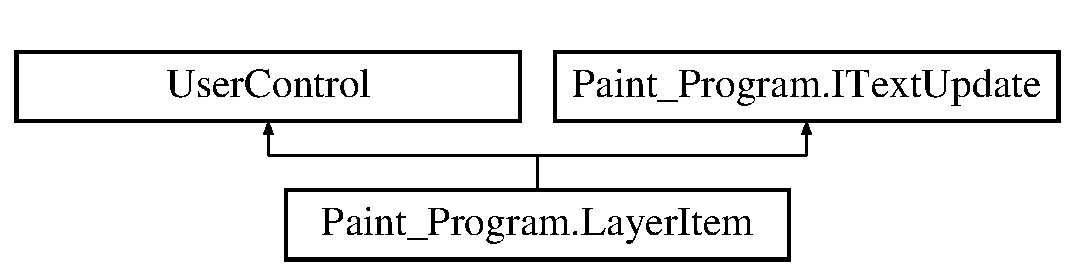
\includegraphics[height=2.000000cm]{class_paint___program_1_1_layer_item}
\end{center}
\end{figure}
\subsection*{Public Member Functions}
\begin{DoxyCompactItemize}
\item 
\mbox{\hyperlink{class_paint___program_1_1_layer_item_ad6222eb0d085d1534ea611e9459a8625}{Layer\+Item}} (int w, int h, Pixel\+Format pf, String name)
\item 
void \mbox{\hyperlink{class_paint___program_1_1_layer_item_ae96f2092c93cd2f38cdcf9a923e45ff3}{update\+Preview}} ()
\item 
void \mbox{\hyperlink{class_paint___program_1_1_layer_item_a649977d6df5ecf05e1ddf57ed1724bff}{update\+Settings}} ()
\item 
Graphics \mbox{\hyperlink{class_paint___program_1_1_layer_item_aaaa8ad207673d7db20deb9a084b2a3e3}{get\+Graphics}} ()
\item 
Bitmap \mbox{\hyperlink{class_paint___program_1_1_layer_item_a3055f80c0799ba9d800513881b866f56}{get\+Bitmap}} ()
\item 
void \mbox{\hyperlink{class_paint___program_1_1_layer_item_a0cdb47e3de7f09a88df2a3ee7e3e1f2a}{set\+Bitmap}} (Bitmap b)
\item 
void \mbox{\hyperlink{class_paint___program_1_1_layer_item_af4e60cbe11c705aff29929704c8be6b3}{set\+Active}} (bool f)
\item 
void \mbox{\hyperlink{class_paint___program_1_1_layer_item_ac87042bbaa15bd3c798db8033c6e2b1f}{set\+Visibility}} (bool f)
\item 
bool \mbox{\hyperlink{class_paint___program_1_1_layer_item_a1c0d40a9d83be0d34ec6c9573fc9a8f0}{is\+Layer\+Visible}} ()
\item 
bool \mbox{\hyperlink{class_paint___program_1_1_layer_item_ae6e321929763123db3137f0e23146bbe}{is\+Layer\+Active}} ()
\item 
String \mbox{\hyperlink{class_paint___program_1_1_layer_item_a99f0895f89d20e4d03fd5937a3b7f794}{get\+Layer\+Name}} ()
\item 
void \mbox{\hyperlink{class_paint___program_1_1_layer_item_a862b3f58efec4a13a07c422a5589ba7c}{set\+On\+Click}} (System.\+Event\+Handler func)
\item 
void \mbox{\hyperlink{class_paint___program_1_1_layer_item_a7cbff967883c3895e000050a5c6e2144}{Update\+Text}} ()
\end{DoxyCompactItemize}
\subsection*{Protected Member Functions}
\begin{DoxyCompactItemize}
\item 
override void \mbox{\hyperlink{class_paint___program_1_1_layer_item_a2d910d24422666826cf1d8b14b35c2d8}{Dispose}} (bool disposing)
\begin{DoxyCompactList}\small\item\em Clean up any resources being used. \end{DoxyCompactList}\end{DoxyCompactItemize}
\subsection*{Private Member Functions}
\begin{DoxyCompactItemize}
\item 
void \mbox{\hyperlink{class_paint___program_1_1_layer_item_a30d692ca1e4a7904c71901f42e615195}{update\+Color}} ()
\item 
void \mbox{\hyperlink{class_paint___program_1_1_layer_item_a28d83ed5185a05aef8881a747be998c5}{cb\+Visible\+\_\+\+Checked\+Changed}} (object sender, Event\+Args e)
\item 
void \mbox{\hyperlink{class_paint___program_1_1_layer_item_a0e322beb67184d03159c83c51a9d4f18}{pb\+Layer\+Preview\+\_\+\+Click}} (object sender, Event\+Args e)
\item 
void \mbox{\hyperlink{class_paint___program_1_1_layer_item_a1ebd3bed165ce47d5530ca2ea2231aa3}{Layer\+Form\+\_\+\+Click}} (object sender, Event\+Args e)
\item 
void \mbox{\hyperlink{class_paint___program_1_1_layer_item_adb9c7138bcc3b99d1e5a53d3c7a81158}{tb\+Layer\+Name\+\_\+\+Click}} (object sender, Event\+Args e)
\item 
void \mbox{\hyperlink{class_paint___program_1_1_layer_item_aac19726d3b27cc9f8d8555140f78a367}{tb\+Layer\+Name\+\_\+\+Key\+Down}} (object sender, Key\+Event\+Args e)
\item 
void \mbox{\hyperlink{class_paint___program_1_1_layer_item_ad2a0b5d51790855d5f254b0d0fa118e3}{tb\+Layer\+Name\+\_\+\+Text\+Changed}} (object sender, Event\+Args e)
\item 
void \mbox{\hyperlink{class_paint___program_1_1_layer_item_a15df54e7a31385d6eb90d78709187fee}{Initialize\+Component}} ()
\begin{DoxyCompactList}\small\item\em Required method for Designer support -\/ do not modify the contents of this method with the code editor. \end{DoxyCompactList}\end{DoxyCompactItemize}
\subsection*{Private Attributes}
\begin{DoxyCompactItemize}
\item 
bool \mbox{\hyperlink{class_paint___program_1_1_layer_item_a150bf0886b6825b2162abcd707c39848}{is\+Visible}}
\item 
bool \mbox{\hyperlink{class_paint___program_1_1_layer_item_addf7b242ff430f0ae633e4f9a856f463}{is\+Active}}
\item 
String \mbox{\hyperlink{class_paint___program_1_1_layer_item_ac449b2dc7a9ace5fa018c50fc910afe8}{s\+Layer\+Name}}
\item 
Color \mbox{\hyperlink{class_paint___program_1_1_layer_item_a0d48969f95aa232f5e87412b661368f5}{c\+Active}} = Color.\+From\+Argb(40, 163, 119)
\item 
Color \mbox{\hyperlink{class_paint___program_1_1_layer_item_aefd1a426e5a2981f190a699794ddb479}{c\+Not\+Active}} = Color.\+From\+Argb(192, 192, 192)
\item 
Bitmap \mbox{\hyperlink{class_paint___program_1_1_layer_item_a5e7e5d7c82b937b63884b5027ff49817}{Layer\+Bitmap}}
\item 
Graphics \mbox{\hyperlink{class_paint___program_1_1_layer_item_a584d163cf86fefce3ca93a653b3fafc2}{g}}
\item 
System.\+Component\+Model.\+I\+Container \mbox{\hyperlink{class_paint___program_1_1_layer_item_a361143e7af0368cca3162aafcccabf01}{components}} = null
\begin{DoxyCompactList}\small\item\em Required designer variable. \end{DoxyCompactList}\item 
System.\+Windows.\+Forms.\+Check\+Box \mbox{\hyperlink{class_paint___program_1_1_layer_item_a5388fefaa9bf456c098721f3f646ee37}{cb\+Visible}}
\item 
System.\+Windows.\+Forms.\+Picture\+Box \mbox{\hyperlink{class_paint___program_1_1_layer_item_a01edbd43c44469ca11c2e8e7e369c55d}{pb\+Layer\+Preview}}
\item 
System.\+Windows.\+Forms.\+Text\+Box \mbox{\hyperlink{class_paint___program_1_1_layer_item_abb01dd9209b972c3ed47cc841a156eb1}{tb\+Layer\+Name}}
\end{DoxyCompactItemize}


\subsection{Constructor \& Destructor Documentation}
\mbox{\Hypertarget{class_paint___program_1_1_layer_item_ad6222eb0d085d1534ea611e9459a8625}\label{class_paint___program_1_1_layer_item_ad6222eb0d085d1534ea611e9459a8625}} 
\index{Paint\+\_\+\+Program\+::\+Layer\+Item@{Paint\+\_\+\+Program\+::\+Layer\+Item}!Layer\+Item@{Layer\+Item}}
\index{Layer\+Item@{Layer\+Item}!Paint\+\_\+\+Program\+::\+Layer\+Item@{Paint\+\_\+\+Program\+::\+Layer\+Item}}
\subsubsection{\texorpdfstring{Layer\+Item()}{LayerItem()}}
{\footnotesize\ttfamily Paint\+\_\+\+Program.\+Layer\+Item.\+Layer\+Item (\begin{DoxyParamCaption}\item[{int}]{w,  }\item[{int}]{h,  }\item[{Pixel\+Format}]{pf,  }\item[{String}]{name }\end{DoxyParamCaption})\hspace{0.3cm}{\ttfamily [inline]}}



\subsection{Member Function Documentation}
\mbox{\Hypertarget{class_paint___program_1_1_layer_item_a28d83ed5185a05aef8881a747be998c5}\label{class_paint___program_1_1_layer_item_a28d83ed5185a05aef8881a747be998c5}} 
\index{Paint\+\_\+\+Program\+::\+Layer\+Item@{Paint\+\_\+\+Program\+::\+Layer\+Item}!cb\+Visible\+\_\+\+Checked\+Changed@{cb\+Visible\+\_\+\+Checked\+Changed}}
\index{cb\+Visible\+\_\+\+Checked\+Changed@{cb\+Visible\+\_\+\+Checked\+Changed}!Paint\+\_\+\+Program\+::\+Layer\+Item@{Paint\+\_\+\+Program\+::\+Layer\+Item}}
\subsubsection{\texorpdfstring{cb\+Visible\+\_\+\+Checked\+Changed()}{cbVisible\_CheckedChanged()}}
{\footnotesize\ttfamily void Paint\+\_\+\+Program.\+Layer\+Item.\+cb\+Visible\+\_\+\+Checked\+Changed (\begin{DoxyParamCaption}\item[{object}]{sender,  }\item[{Event\+Args}]{e }\end{DoxyParamCaption})\hspace{0.3cm}{\ttfamily [inline]}, {\ttfamily [private]}}

\mbox{\Hypertarget{class_paint___program_1_1_layer_item_a2d910d24422666826cf1d8b14b35c2d8}\label{class_paint___program_1_1_layer_item_a2d910d24422666826cf1d8b14b35c2d8}} 
\index{Paint\+\_\+\+Program\+::\+Layer\+Item@{Paint\+\_\+\+Program\+::\+Layer\+Item}!Dispose@{Dispose}}
\index{Dispose@{Dispose}!Paint\+\_\+\+Program\+::\+Layer\+Item@{Paint\+\_\+\+Program\+::\+Layer\+Item}}
\subsubsection{\texorpdfstring{Dispose()}{Dispose()}}
{\footnotesize\ttfamily override void Paint\+\_\+\+Program.\+Layer\+Item.\+Dispose (\begin{DoxyParamCaption}\item[{bool}]{disposing }\end{DoxyParamCaption})\hspace{0.3cm}{\ttfamily [inline]}, {\ttfamily [protected]}}



Clean up any resources being used. 


\begin{DoxyParams}{Parameters}
{\em disposing} & true if managed resources should be disposed; otherwise, false.\\
\hline
\end{DoxyParams}
\mbox{\Hypertarget{class_paint___program_1_1_layer_item_a3055f80c0799ba9d800513881b866f56}\label{class_paint___program_1_1_layer_item_a3055f80c0799ba9d800513881b866f56}} 
\index{Paint\+\_\+\+Program\+::\+Layer\+Item@{Paint\+\_\+\+Program\+::\+Layer\+Item}!get\+Bitmap@{get\+Bitmap}}
\index{get\+Bitmap@{get\+Bitmap}!Paint\+\_\+\+Program\+::\+Layer\+Item@{Paint\+\_\+\+Program\+::\+Layer\+Item}}
\subsubsection{\texorpdfstring{get\+Bitmap()}{getBitmap()}}
{\footnotesize\ttfamily Bitmap Paint\+\_\+\+Program.\+Layer\+Item.\+get\+Bitmap (\begin{DoxyParamCaption}{ }\end{DoxyParamCaption})\hspace{0.3cm}{\ttfamily [inline]}}

\mbox{\Hypertarget{class_paint___program_1_1_layer_item_aaaa8ad207673d7db20deb9a084b2a3e3}\label{class_paint___program_1_1_layer_item_aaaa8ad207673d7db20deb9a084b2a3e3}} 
\index{Paint\+\_\+\+Program\+::\+Layer\+Item@{Paint\+\_\+\+Program\+::\+Layer\+Item}!get\+Graphics@{get\+Graphics}}
\index{get\+Graphics@{get\+Graphics}!Paint\+\_\+\+Program\+::\+Layer\+Item@{Paint\+\_\+\+Program\+::\+Layer\+Item}}
\subsubsection{\texorpdfstring{get\+Graphics()}{getGraphics()}}
{\footnotesize\ttfamily Graphics Paint\+\_\+\+Program.\+Layer\+Item.\+get\+Graphics (\begin{DoxyParamCaption}{ }\end{DoxyParamCaption})\hspace{0.3cm}{\ttfamily [inline]}}

\mbox{\Hypertarget{class_paint___program_1_1_layer_item_a99f0895f89d20e4d03fd5937a3b7f794}\label{class_paint___program_1_1_layer_item_a99f0895f89d20e4d03fd5937a3b7f794}} 
\index{Paint\+\_\+\+Program\+::\+Layer\+Item@{Paint\+\_\+\+Program\+::\+Layer\+Item}!get\+Layer\+Name@{get\+Layer\+Name}}
\index{get\+Layer\+Name@{get\+Layer\+Name}!Paint\+\_\+\+Program\+::\+Layer\+Item@{Paint\+\_\+\+Program\+::\+Layer\+Item}}
\subsubsection{\texorpdfstring{get\+Layer\+Name()}{getLayerName()}}
{\footnotesize\ttfamily String Paint\+\_\+\+Program.\+Layer\+Item.\+get\+Layer\+Name (\begin{DoxyParamCaption}{ }\end{DoxyParamCaption})\hspace{0.3cm}{\ttfamily [inline]}}

\mbox{\Hypertarget{class_paint___program_1_1_layer_item_a15df54e7a31385d6eb90d78709187fee}\label{class_paint___program_1_1_layer_item_a15df54e7a31385d6eb90d78709187fee}} 
\index{Paint\+\_\+\+Program\+::\+Layer\+Item@{Paint\+\_\+\+Program\+::\+Layer\+Item}!Initialize\+Component@{Initialize\+Component}}
\index{Initialize\+Component@{Initialize\+Component}!Paint\+\_\+\+Program\+::\+Layer\+Item@{Paint\+\_\+\+Program\+::\+Layer\+Item}}
\subsubsection{\texorpdfstring{Initialize\+Component()}{InitializeComponent()}}
{\footnotesize\ttfamily void Paint\+\_\+\+Program.\+Layer\+Item.\+Initialize\+Component (\begin{DoxyParamCaption}{ }\end{DoxyParamCaption})\hspace{0.3cm}{\ttfamily [inline]}, {\ttfamily [private]}}



Required method for Designer support -\/ do not modify the contents of this method with the code editor. 

\mbox{\Hypertarget{class_paint___program_1_1_layer_item_ae6e321929763123db3137f0e23146bbe}\label{class_paint___program_1_1_layer_item_ae6e321929763123db3137f0e23146bbe}} 
\index{Paint\+\_\+\+Program\+::\+Layer\+Item@{Paint\+\_\+\+Program\+::\+Layer\+Item}!is\+Layer\+Active@{is\+Layer\+Active}}
\index{is\+Layer\+Active@{is\+Layer\+Active}!Paint\+\_\+\+Program\+::\+Layer\+Item@{Paint\+\_\+\+Program\+::\+Layer\+Item}}
\subsubsection{\texorpdfstring{is\+Layer\+Active()}{isLayerActive()}}
{\footnotesize\ttfamily bool Paint\+\_\+\+Program.\+Layer\+Item.\+is\+Layer\+Active (\begin{DoxyParamCaption}{ }\end{DoxyParamCaption})\hspace{0.3cm}{\ttfamily [inline]}}

\mbox{\Hypertarget{class_paint___program_1_1_layer_item_a1c0d40a9d83be0d34ec6c9573fc9a8f0}\label{class_paint___program_1_1_layer_item_a1c0d40a9d83be0d34ec6c9573fc9a8f0}} 
\index{Paint\+\_\+\+Program\+::\+Layer\+Item@{Paint\+\_\+\+Program\+::\+Layer\+Item}!is\+Layer\+Visible@{is\+Layer\+Visible}}
\index{is\+Layer\+Visible@{is\+Layer\+Visible}!Paint\+\_\+\+Program\+::\+Layer\+Item@{Paint\+\_\+\+Program\+::\+Layer\+Item}}
\subsubsection{\texorpdfstring{is\+Layer\+Visible()}{isLayerVisible()}}
{\footnotesize\ttfamily bool Paint\+\_\+\+Program.\+Layer\+Item.\+is\+Layer\+Visible (\begin{DoxyParamCaption}{ }\end{DoxyParamCaption})\hspace{0.3cm}{\ttfamily [inline]}}

\mbox{\Hypertarget{class_paint___program_1_1_layer_item_a1ebd3bed165ce47d5530ca2ea2231aa3}\label{class_paint___program_1_1_layer_item_a1ebd3bed165ce47d5530ca2ea2231aa3}} 
\index{Paint\+\_\+\+Program\+::\+Layer\+Item@{Paint\+\_\+\+Program\+::\+Layer\+Item}!Layer\+Form\+\_\+\+Click@{Layer\+Form\+\_\+\+Click}}
\index{Layer\+Form\+\_\+\+Click@{Layer\+Form\+\_\+\+Click}!Paint\+\_\+\+Program\+::\+Layer\+Item@{Paint\+\_\+\+Program\+::\+Layer\+Item}}
\subsubsection{\texorpdfstring{Layer\+Form\+\_\+\+Click()}{LayerForm\_Click()}}
{\footnotesize\ttfamily void Paint\+\_\+\+Program.\+Layer\+Item.\+Layer\+Form\+\_\+\+Click (\begin{DoxyParamCaption}\item[{object}]{sender,  }\item[{Event\+Args}]{e }\end{DoxyParamCaption})\hspace{0.3cm}{\ttfamily [inline]}, {\ttfamily [private]}}

\mbox{\Hypertarget{class_paint___program_1_1_layer_item_a0e322beb67184d03159c83c51a9d4f18}\label{class_paint___program_1_1_layer_item_a0e322beb67184d03159c83c51a9d4f18}} 
\index{Paint\+\_\+\+Program\+::\+Layer\+Item@{Paint\+\_\+\+Program\+::\+Layer\+Item}!pb\+Layer\+Preview\+\_\+\+Click@{pb\+Layer\+Preview\+\_\+\+Click}}
\index{pb\+Layer\+Preview\+\_\+\+Click@{pb\+Layer\+Preview\+\_\+\+Click}!Paint\+\_\+\+Program\+::\+Layer\+Item@{Paint\+\_\+\+Program\+::\+Layer\+Item}}
\subsubsection{\texorpdfstring{pb\+Layer\+Preview\+\_\+\+Click()}{pbLayerPreview\_Click()}}
{\footnotesize\ttfamily void Paint\+\_\+\+Program.\+Layer\+Item.\+pb\+Layer\+Preview\+\_\+\+Click (\begin{DoxyParamCaption}\item[{object}]{sender,  }\item[{Event\+Args}]{e }\end{DoxyParamCaption})\hspace{0.3cm}{\ttfamily [inline]}, {\ttfamily [private]}}

\mbox{\Hypertarget{class_paint___program_1_1_layer_item_af4e60cbe11c705aff29929704c8be6b3}\label{class_paint___program_1_1_layer_item_af4e60cbe11c705aff29929704c8be6b3}} 
\index{Paint\+\_\+\+Program\+::\+Layer\+Item@{Paint\+\_\+\+Program\+::\+Layer\+Item}!set\+Active@{set\+Active}}
\index{set\+Active@{set\+Active}!Paint\+\_\+\+Program\+::\+Layer\+Item@{Paint\+\_\+\+Program\+::\+Layer\+Item}}
\subsubsection{\texorpdfstring{set\+Active()}{setActive()}}
{\footnotesize\ttfamily void Paint\+\_\+\+Program.\+Layer\+Item.\+set\+Active (\begin{DoxyParamCaption}\item[{bool}]{f }\end{DoxyParamCaption})\hspace{0.3cm}{\ttfamily [inline]}}

\mbox{\Hypertarget{class_paint___program_1_1_layer_item_a0cdb47e3de7f09a88df2a3ee7e3e1f2a}\label{class_paint___program_1_1_layer_item_a0cdb47e3de7f09a88df2a3ee7e3e1f2a}} 
\index{Paint\+\_\+\+Program\+::\+Layer\+Item@{Paint\+\_\+\+Program\+::\+Layer\+Item}!set\+Bitmap@{set\+Bitmap}}
\index{set\+Bitmap@{set\+Bitmap}!Paint\+\_\+\+Program\+::\+Layer\+Item@{Paint\+\_\+\+Program\+::\+Layer\+Item}}
\subsubsection{\texorpdfstring{set\+Bitmap()}{setBitmap()}}
{\footnotesize\ttfamily void Paint\+\_\+\+Program.\+Layer\+Item.\+set\+Bitmap (\begin{DoxyParamCaption}\item[{Bitmap}]{b }\end{DoxyParamCaption})\hspace{0.3cm}{\ttfamily [inline]}}

\mbox{\Hypertarget{class_paint___program_1_1_layer_item_a862b3f58efec4a13a07c422a5589ba7c}\label{class_paint___program_1_1_layer_item_a862b3f58efec4a13a07c422a5589ba7c}} 
\index{Paint\+\_\+\+Program\+::\+Layer\+Item@{Paint\+\_\+\+Program\+::\+Layer\+Item}!set\+On\+Click@{set\+On\+Click}}
\index{set\+On\+Click@{set\+On\+Click}!Paint\+\_\+\+Program\+::\+Layer\+Item@{Paint\+\_\+\+Program\+::\+Layer\+Item}}
\subsubsection{\texorpdfstring{set\+On\+Click()}{setOnClick()}}
{\footnotesize\ttfamily void Paint\+\_\+\+Program.\+Layer\+Item.\+set\+On\+Click (\begin{DoxyParamCaption}\item[{System.\+Event\+Handler}]{func }\end{DoxyParamCaption})\hspace{0.3cm}{\ttfamily [inline]}}

\mbox{\Hypertarget{class_paint___program_1_1_layer_item_ac87042bbaa15bd3c798db8033c6e2b1f}\label{class_paint___program_1_1_layer_item_ac87042bbaa15bd3c798db8033c6e2b1f}} 
\index{Paint\+\_\+\+Program\+::\+Layer\+Item@{Paint\+\_\+\+Program\+::\+Layer\+Item}!set\+Visibility@{set\+Visibility}}
\index{set\+Visibility@{set\+Visibility}!Paint\+\_\+\+Program\+::\+Layer\+Item@{Paint\+\_\+\+Program\+::\+Layer\+Item}}
\subsubsection{\texorpdfstring{set\+Visibility()}{setVisibility()}}
{\footnotesize\ttfamily void Paint\+\_\+\+Program.\+Layer\+Item.\+set\+Visibility (\begin{DoxyParamCaption}\item[{bool}]{f }\end{DoxyParamCaption})\hspace{0.3cm}{\ttfamily [inline]}}

\mbox{\Hypertarget{class_paint___program_1_1_layer_item_adb9c7138bcc3b99d1e5a53d3c7a81158}\label{class_paint___program_1_1_layer_item_adb9c7138bcc3b99d1e5a53d3c7a81158}} 
\index{Paint\+\_\+\+Program\+::\+Layer\+Item@{Paint\+\_\+\+Program\+::\+Layer\+Item}!tb\+Layer\+Name\+\_\+\+Click@{tb\+Layer\+Name\+\_\+\+Click}}
\index{tb\+Layer\+Name\+\_\+\+Click@{tb\+Layer\+Name\+\_\+\+Click}!Paint\+\_\+\+Program\+::\+Layer\+Item@{Paint\+\_\+\+Program\+::\+Layer\+Item}}
\subsubsection{\texorpdfstring{tb\+Layer\+Name\+\_\+\+Click()}{tbLayerName\_Click()}}
{\footnotesize\ttfamily void Paint\+\_\+\+Program.\+Layer\+Item.\+tb\+Layer\+Name\+\_\+\+Click (\begin{DoxyParamCaption}\item[{object}]{sender,  }\item[{Event\+Args}]{e }\end{DoxyParamCaption})\hspace{0.3cm}{\ttfamily [inline]}, {\ttfamily [private]}}

\mbox{\Hypertarget{class_paint___program_1_1_layer_item_aac19726d3b27cc9f8d8555140f78a367}\label{class_paint___program_1_1_layer_item_aac19726d3b27cc9f8d8555140f78a367}} 
\index{Paint\+\_\+\+Program\+::\+Layer\+Item@{Paint\+\_\+\+Program\+::\+Layer\+Item}!tb\+Layer\+Name\+\_\+\+Key\+Down@{tb\+Layer\+Name\+\_\+\+Key\+Down}}
\index{tb\+Layer\+Name\+\_\+\+Key\+Down@{tb\+Layer\+Name\+\_\+\+Key\+Down}!Paint\+\_\+\+Program\+::\+Layer\+Item@{Paint\+\_\+\+Program\+::\+Layer\+Item}}
\subsubsection{\texorpdfstring{tb\+Layer\+Name\+\_\+\+Key\+Down()}{tbLayerName\_KeyDown()}}
{\footnotesize\ttfamily void Paint\+\_\+\+Program.\+Layer\+Item.\+tb\+Layer\+Name\+\_\+\+Key\+Down (\begin{DoxyParamCaption}\item[{object}]{sender,  }\item[{Key\+Event\+Args}]{e }\end{DoxyParamCaption})\hspace{0.3cm}{\ttfamily [inline]}, {\ttfamily [private]}}

\mbox{\Hypertarget{class_paint___program_1_1_layer_item_ad2a0b5d51790855d5f254b0d0fa118e3}\label{class_paint___program_1_1_layer_item_ad2a0b5d51790855d5f254b0d0fa118e3}} 
\index{Paint\+\_\+\+Program\+::\+Layer\+Item@{Paint\+\_\+\+Program\+::\+Layer\+Item}!tb\+Layer\+Name\+\_\+\+Text\+Changed@{tb\+Layer\+Name\+\_\+\+Text\+Changed}}
\index{tb\+Layer\+Name\+\_\+\+Text\+Changed@{tb\+Layer\+Name\+\_\+\+Text\+Changed}!Paint\+\_\+\+Program\+::\+Layer\+Item@{Paint\+\_\+\+Program\+::\+Layer\+Item}}
\subsubsection{\texorpdfstring{tb\+Layer\+Name\+\_\+\+Text\+Changed()}{tbLayerName\_TextChanged()}}
{\footnotesize\ttfamily void Paint\+\_\+\+Program.\+Layer\+Item.\+tb\+Layer\+Name\+\_\+\+Text\+Changed (\begin{DoxyParamCaption}\item[{object}]{sender,  }\item[{Event\+Args}]{e }\end{DoxyParamCaption})\hspace{0.3cm}{\ttfamily [inline]}, {\ttfamily [private]}}

\mbox{\Hypertarget{class_paint___program_1_1_layer_item_a30d692ca1e4a7904c71901f42e615195}\label{class_paint___program_1_1_layer_item_a30d692ca1e4a7904c71901f42e615195}} 
\index{Paint\+\_\+\+Program\+::\+Layer\+Item@{Paint\+\_\+\+Program\+::\+Layer\+Item}!update\+Color@{update\+Color}}
\index{update\+Color@{update\+Color}!Paint\+\_\+\+Program\+::\+Layer\+Item@{Paint\+\_\+\+Program\+::\+Layer\+Item}}
\subsubsection{\texorpdfstring{update\+Color()}{updateColor()}}
{\footnotesize\ttfamily void Paint\+\_\+\+Program.\+Layer\+Item.\+update\+Color (\begin{DoxyParamCaption}{ }\end{DoxyParamCaption})\hspace{0.3cm}{\ttfamily [inline]}, {\ttfamily [private]}}

\mbox{\Hypertarget{class_paint___program_1_1_layer_item_ae96f2092c93cd2f38cdcf9a923e45ff3}\label{class_paint___program_1_1_layer_item_ae96f2092c93cd2f38cdcf9a923e45ff3}} 
\index{Paint\+\_\+\+Program\+::\+Layer\+Item@{Paint\+\_\+\+Program\+::\+Layer\+Item}!update\+Preview@{update\+Preview}}
\index{update\+Preview@{update\+Preview}!Paint\+\_\+\+Program\+::\+Layer\+Item@{Paint\+\_\+\+Program\+::\+Layer\+Item}}
\subsubsection{\texorpdfstring{update\+Preview()}{updatePreview()}}
{\footnotesize\ttfamily void Paint\+\_\+\+Program.\+Layer\+Item.\+update\+Preview (\begin{DoxyParamCaption}{ }\end{DoxyParamCaption})\hspace{0.3cm}{\ttfamily [inline]}}

\mbox{\Hypertarget{class_paint___program_1_1_layer_item_a649977d6df5ecf05e1ddf57ed1724bff}\label{class_paint___program_1_1_layer_item_a649977d6df5ecf05e1ddf57ed1724bff}} 
\index{Paint\+\_\+\+Program\+::\+Layer\+Item@{Paint\+\_\+\+Program\+::\+Layer\+Item}!update\+Settings@{update\+Settings}}
\index{update\+Settings@{update\+Settings}!Paint\+\_\+\+Program\+::\+Layer\+Item@{Paint\+\_\+\+Program\+::\+Layer\+Item}}
\subsubsection{\texorpdfstring{update\+Settings()}{updateSettings()}}
{\footnotesize\ttfamily void Paint\+\_\+\+Program.\+Layer\+Item.\+update\+Settings (\begin{DoxyParamCaption}{ }\end{DoxyParamCaption})\hspace{0.3cm}{\ttfamily [inline]}}

\mbox{\Hypertarget{class_paint___program_1_1_layer_item_a7cbff967883c3895e000050a5c6e2144}\label{class_paint___program_1_1_layer_item_a7cbff967883c3895e000050a5c6e2144}} 
\index{Paint\+\_\+\+Program\+::\+Layer\+Item@{Paint\+\_\+\+Program\+::\+Layer\+Item}!Update\+Text@{Update\+Text}}
\index{Update\+Text@{Update\+Text}!Paint\+\_\+\+Program\+::\+Layer\+Item@{Paint\+\_\+\+Program\+::\+Layer\+Item}}
\subsubsection{\texorpdfstring{Update\+Text()}{UpdateText()}}
{\footnotesize\ttfamily void Paint\+\_\+\+Program.\+Layer\+Item.\+Update\+Text (\begin{DoxyParamCaption}{ }\end{DoxyParamCaption})\hspace{0.3cm}{\ttfamily [inline]}}



Implements \mbox{\hyperlink{interface_paint___program_1_1_i_text_update_ad1e94db137571608917117e9a6f7479b}{Paint\+\_\+\+Program.\+I\+Text\+Update}}.



\subsection{Member Data Documentation}
\mbox{\Hypertarget{class_paint___program_1_1_layer_item_a0d48969f95aa232f5e87412b661368f5}\label{class_paint___program_1_1_layer_item_a0d48969f95aa232f5e87412b661368f5}} 
\index{Paint\+\_\+\+Program\+::\+Layer\+Item@{Paint\+\_\+\+Program\+::\+Layer\+Item}!c\+Active@{c\+Active}}
\index{c\+Active@{c\+Active}!Paint\+\_\+\+Program\+::\+Layer\+Item@{Paint\+\_\+\+Program\+::\+Layer\+Item}}
\subsubsection{\texorpdfstring{c\+Active}{cActive}}
{\footnotesize\ttfamily Color Paint\+\_\+\+Program.\+Layer\+Item.\+c\+Active = Color.\+From\+Argb(40, 163, 119)\hspace{0.3cm}{\ttfamily [private]}}

\mbox{\Hypertarget{class_paint___program_1_1_layer_item_a5388fefaa9bf456c098721f3f646ee37}\label{class_paint___program_1_1_layer_item_a5388fefaa9bf456c098721f3f646ee37}} 
\index{Paint\+\_\+\+Program\+::\+Layer\+Item@{Paint\+\_\+\+Program\+::\+Layer\+Item}!cb\+Visible@{cb\+Visible}}
\index{cb\+Visible@{cb\+Visible}!Paint\+\_\+\+Program\+::\+Layer\+Item@{Paint\+\_\+\+Program\+::\+Layer\+Item}}
\subsubsection{\texorpdfstring{cb\+Visible}{cbVisible}}
{\footnotesize\ttfamily System.\+Windows.\+Forms.\+Check\+Box Paint\+\_\+\+Program.\+Layer\+Item.\+cb\+Visible\hspace{0.3cm}{\ttfamily [private]}}

\mbox{\Hypertarget{class_paint___program_1_1_layer_item_aefd1a426e5a2981f190a699794ddb479}\label{class_paint___program_1_1_layer_item_aefd1a426e5a2981f190a699794ddb479}} 
\index{Paint\+\_\+\+Program\+::\+Layer\+Item@{Paint\+\_\+\+Program\+::\+Layer\+Item}!c\+Not\+Active@{c\+Not\+Active}}
\index{c\+Not\+Active@{c\+Not\+Active}!Paint\+\_\+\+Program\+::\+Layer\+Item@{Paint\+\_\+\+Program\+::\+Layer\+Item}}
\subsubsection{\texorpdfstring{c\+Not\+Active}{cNotActive}}
{\footnotesize\ttfamily Color Paint\+\_\+\+Program.\+Layer\+Item.\+c\+Not\+Active = Color.\+From\+Argb(192, 192, 192)\hspace{0.3cm}{\ttfamily [private]}}

\mbox{\Hypertarget{class_paint___program_1_1_layer_item_a361143e7af0368cca3162aafcccabf01}\label{class_paint___program_1_1_layer_item_a361143e7af0368cca3162aafcccabf01}} 
\index{Paint\+\_\+\+Program\+::\+Layer\+Item@{Paint\+\_\+\+Program\+::\+Layer\+Item}!components@{components}}
\index{components@{components}!Paint\+\_\+\+Program\+::\+Layer\+Item@{Paint\+\_\+\+Program\+::\+Layer\+Item}}
\subsubsection{\texorpdfstring{components}{components}}
{\footnotesize\ttfamily System.\+Component\+Model.\+I\+Container Paint\+\_\+\+Program.\+Layer\+Item.\+components = null\hspace{0.3cm}{\ttfamily [private]}}



Required designer variable. 

\mbox{\Hypertarget{class_paint___program_1_1_layer_item_a584d163cf86fefce3ca93a653b3fafc2}\label{class_paint___program_1_1_layer_item_a584d163cf86fefce3ca93a653b3fafc2}} 
\index{Paint\+\_\+\+Program\+::\+Layer\+Item@{Paint\+\_\+\+Program\+::\+Layer\+Item}!g@{g}}
\index{g@{g}!Paint\+\_\+\+Program\+::\+Layer\+Item@{Paint\+\_\+\+Program\+::\+Layer\+Item}}
\subsubsection{\texorpdfstring{g}{g}}
{\footnotesize\ttfamily Graphics Paint\+\_\+\+Program.\+Layer\+Item.\+g\hspace{0.3cm}{\ttfamily [private]}}

\mbox{\Hypertarget{class_paint___program_1_1_layer_item_addf7b242ff430f0ae633e4f9a856f463}\label{class_paint___program_1_1_layer_item_addf7b242ff430f0ae633e4f9a856f463}} 
\index{Paint\+\_\+\+Program\+::\+Layer\+Item@{Paint\+\_\+\+Program\+::\+Layer\+Item}!is\+Active@{is\+Active}}
\index{is\+Active@{is\+Active}!Paint\+\_\+\+Program\+::\+Layer\+Item@{Paint\+\_\+\+Program\+::\+Layer\+Item}}
\subsubsection{\texorpdfstring{is\+Active}{isActive}}
{\footnotesize\ttfamily bool Paint\+\_\+\+Program.\+Layer\+Item.\+is\+Active\hspace{0.3cm}{\ttfamily [private]}}

\mbox{\Hypertarget{class_paint___program_1_1_layer_item_a150bf0886b6825b2162abcd707c39848}\label{class_paint___program_1_1_layer_item_a150bf0886b6825b2162abcd707c39848}} 
\index{Paint\+\_\+\+Program\+::\+Layer\+Item@{Paint\+\_\+\+Program\+::\+Layer\+Item}!is\+Visible@{is\+Visible}}
\index{is\+Visible@{is\+Visible}!Paint\+\_\+\+Program\+::\+Layer\+Item@{Paint\+\_\+\+Program\+::\+Layer\+Item}}
\subsubsection{\texorpdfstring{is\+Visible}{isVisible}}
{\footnotesize\ttfamily bool Paint\+\_\+\+Program.\+Layer\+Item.\+is\+Visible\hspace{0.3cm}{\ttfamily [private]}}

\mbox{\Hypertarget{class_paint___program_1_1_layer_item_a5e7e5d7c82b937b63884b5027ff49817}\label{class_paint___program_1_1_layer_item_a5e7e5d7c82b937b63884b5027ff49817}} 
\index{Paint\+\_\+\+Program\+::\+Layer\+Item@{Paint\+\_\+\+Program\+::\+Layer\+Item}!Layer\+Bitmap@{Layer\+Bitmap}}
\index{Layer\+Bitmap@{Layer\+Bitmap}!Paint\+\_\+\+Program\+::\+Layer\+Item@{Paint\+\_\+\+Program\+::\+Layer\+Item}}
\subsubsection{\texorpdfstring{Layer\+Bitmap}{LayerBitmap}}
{\footnotesize\ttfamily Bitmap Paint\+\_\+\+Program.\+Layer\+Item.\+Layer\+Bitmap\hspace{0.3cm}{\ttfamily [private]}}

\mbox{\Hypertarget{class_paint___program_1_1_layer_item_a01edbd43c44469ca11c2e8e7e369c55d}\label{class_paint___program_1_1_layer_item_a01edbd43c44469ca11c2e8e7e369c55d}} 
\index{Paint\+\_\+\+Program\+::\+Layer\+Item@{Paint\+\_\+\+Program\+::\+Layer\+Item}!pb\+Layer\+Preview@{pb\+Layer\+Preview}}
\index{pb\+Layer\+Preview@{pb\+Layer\+Preview}!Paint\+\_\+\+Program\+::\+Layer\+Item@{Paint\+\_\+\+Program\+::\+Layer\+Item}}
\subsubsection{\texorpdfstring{pb\+Layer\+Preview}{pbLayerPreview}}
{\footnotesize\ttfamily System.\+Windows.\+Forms.\+Picture\+Box Paint\+\_\+\+Program.\+Layer\+Item.\+pb\+Layer\+Preview\hspace{0.3cm}{\ttfamily [private]}}

\mbox{\Hypertarget{class_paint___program_1_1_layer_item_ac449b2dc7a9ace5fa018c50fc910afe8}\label{class_paint___program_1_1_layer_item_ac449b2dc7a9ace5fa018c50fc910afe8}} 
\index{Paint\+\_\+\+Program\+::\+Layer\+Item@{Paint\+\_\+\+Program\+::\+Layer\+Item}!s\+Layer\+Name@{s\+Layer\+Name}}
\index{s\+Layer\+Name@{s\+Layer\+Name}!Paint\+\_\+\+Program\+::\+Layer\+Item@{Paint\+\_\+\+Program\+::\+Layer\+Item}}
\subsubsection{\texorpdfstring{s\+Layer\+Name}{sLayerName}}
{\footnotesize\ttfamily String Paint\+\_\+\+Program.\+Layer\+Item.\+s\+Layer\+Name\hspace{0.3cm}{\ttfamily [private]}}

\mbox{\Hypertarget{class_paint___program_1_1_layer_item_abb01dd9209b972c3ed47cc841a156eb1}\label{class_paint___program_1_1_layer_item_abb01dd9209b972c3ed47cc841a156eb1}} 
\index{Paint\+\_\+\+Program\+::\+Layer\+Item@{Paint\+\_\+\+Program\+::\+Layer\+Item}!tb\+Layer\+Name@{tb\+Layer\+Name}}
\index{tb\+Layer\+Name@{tb\+Layer\+Name}!Paint\+\_\+\+Program\+::\+Layer\+Item@{Paint\+\_\+\+Program\+::\+Layer\+Item}}
\subsubsection{\texorpdfstring{tb\+Layer\+Name}{tbLayerName}}
{\footnotesize\ttfamily System.\+Windows.\+Forms.\+Text\+Box Paint\+\_\+\+Program.\+Layer\+Item.\+tb\+Layer\+Name\hspace{0.3cm}{\ttfamily [private]}}



The documentation for this class was generated from the following files\+:\begin{DoxyCompactItemize}
\item 
Paint Program/\mbox{\hyperlink{_layer_item_8cs}{Layer\+Item.\+cs}}\item 
Paint Program/\mbox{\hyperlink{_layer_item_8_designer_8cs}{Layer\+Item.\+Designer.\+cs}}\end{DoxyCompactItemize}

\hypertarget{class_paint___program_1_1_layer_view}{}\section{Paint\+\_\+\+Program.\+Layer\+View Class Reference}
\label{class_paint___program_1_1_layer_view}\index{Paint\+\_\+\+Program.\+Layer\+View@{Paint\+\_\+\+Program.\+Layer\+View}}
Inheritance diagram for Paint\+\_\+\+Program.\+Layer\+View\+:\begin{figure}[H]
\begin{center}
\leavevmode
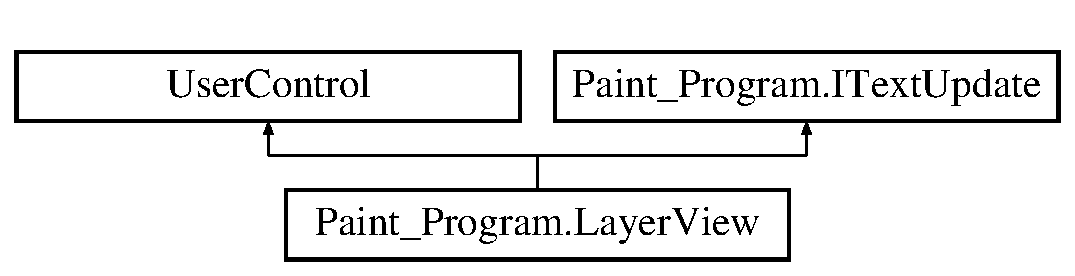
\includegraphics[height=2.000000cm]{class_paint___program_1_1_layer_view}
\end{center}
\end{figure}
\subsection*{Public Member Functions}
\begin{DoxyCompactItemize}
\item 
\mbox{\hyperlink{class_paint___program_1_1_layer_view_a237468f9156f9a2dbdde7692209acb91}{Layer\+View}} (int w, int h)
\item 
void \mbox{\hyperlink{class_paint___program_1_1_layer_view_a4872c0c1b55f0c4a1f842061def219fd}{update\+Active\+Layer}} ()
\item 
void \mbox{\hyperlink{class_paint___program_1_1_layer_view_ad82f5a23e54318684a6ff17b5ee7c32e}{update\+Active\+Layer\+Settings}} ()
\item 
Bitmap \mbox{\hyperlink{class_paint___program_1_1_layer_view_a8d4ff09153310ad7fc153cd45f8ec90d}{get\+Render}} ()
\item 
Graphics \mbox{\hyperlink{class_paint___program_1_1_layer_view_af4347af0118fb18274cfead40ebde85d}{get\+Active\+Layer\+Graphics}} ()
\item 
Bitmap \mbox{\hyperlink{class_paint___program_1_1_layer_view_a782154cc9526719190749ce372e6afdd}{get\+Active\+Layer\+Bitmap}} ()
\item 
\mbox{\hyperlink{class_paint___program_1_1_layer_item}{Layer\+Item}} \mbox{\hyperlink{class_paint___program_1_1_layer_view_ab1d91b912733c8ac3ac51087bde8ac94}{get\+Active\+Layer}} ()
\item 
void \mbox{\hyperlink{class_paint___program_1_1_layer_view_a3a8cf41dfd57b3b755331b2cd411acdb}{Update\+Layer\+Info\+Listener}} ()
\item 
void \mbox{\hyperlink{class_paint___program_1_1_layer_view_aed4ebc6256430120819f0de98d65976b}{add\+Import\+Image}} (Bitmap b)
\item 
void \mbox{\hyperlink{class_paint___program_1_1_layer_view_a8904d504aab68f82088349dba9a06e50}{Grid\+Draw}} (Graphics g)
\item 
void \mbox{\hyperlink{class_paint___program_1_1_layer_view_a0f223144d8d2e7833b530abbeb224f98}{Trash}} ()
\item 
void \mbox{\hyperlink{class_paint___program_1_1_layer_view_a9524e183d6c00b15c217e9d5c1d14aea}{Update\+Text}} ()
\end{DoxyCompactItemize}
\subsection*{Protected Member Functions}
\begin{DoxyCompactItemize}
\item 
override void \mbox{\hyperlink{class_paint___program_1_1_layer_view_a50b056c433212a850e348643339ec504}{Dispose}} (bool disposing)
\begin{DoxyCompactList}\small\item\em Clean up any resources being used. \end{DoxyCompactList}\end{DoxyCompactItemize}
\subsection*{Private Member Functions}
\begin{DoxyCompactItemize}
\item 
void \mbox{\hyperlink{class_paint___program_1_1_layer_view_ae37145bc09093999c35a5ed4cfd0b4f4}{handle\+Mouse\+Wheel}} (object sender, Mouse\+Event\+Args e)
\item 
void \mbox{\hyperlink{class_paint___program_1_1_layer_view_a4f472408447efa4b42636652e8e6543c}{handle\+Scroll}} (object sender, Scroll\+Event\+Args e)
\item 
int \mbox{\hyperlink{class_paint___program_1_1_layer_view_a530e1b907d4d7170ed2bb4458142ab4e}{get\+Active\+Layer\+Index}} ()
\item 
void \mbox{\hyperlink{class_paint___program_1_1_layer_view_a5a79b6f0d42626db4e46740ba7acd3d6}{b\+Add\+Layer\+\_\+\+Click}} (object sender, Event\+Args e)
\item 
void \mbox{\hyperlink{class_paint___program_1_1_layer_view_a9113020298ddd2453ded7a2c9f290f25}{b\+Remove\+Layer\+\_\+\+Click}} (object sender, Event\+Args e)
\item 
void \mbox{\hyperlink{class_paint___program_1_1_layer_view_ae9cf7ac141487ef8296aa8982f36dd4b}{add\+Layer}} ()
\item 
void \mbox{\hyperlink{class_paint___program_1_1_layer_view_aa7d7b70619b86d67ed2e86b94df5da89}{add\+Layer}} (Bitmap b, String name)
\item 
void \mbox{\hyperlink{class_paint___program_1_1_layer_view_ac0005cdabdf8818860cc85ec9a9620c7}{remove\+Layer}} ()
\item 
void \mbox{\hyperlink{class_paint___program_1_1_layer_view_a3aea3b23c16f637b1e71c6e124c0d1ed}{redraw\+Layer\+Items}} ()
\item 
void \mbox{\hyperlink{class_paint___program_1_1_layer_view_ae1c2bd86cca19963e75832b53810f39f}{b\+Move\+Down\+\_\+\+Click}} (object sender, Event\+Args e)
\item 
void \mbox{\hyperlink{class_paint___program_1_1_layer_view_af33e0c3be1c72f6893591068f1735f6c}{b\+Move\+Up\+\_\+\+Click}} (object sender, Event\+Args e)
\item 
void \mbox{\hyperlink{class_paint___program_1_1_layer_view_a61a0b7470102d6ce9f9e306f703aac1a}{handle\+Layer\+Item\+Click}} (object obj, System.\+Event\+Args args)
\item 
void \mbox{\hyperlink{class_paint___program_1_1_layer_view_af4ccbb4bfa3763c0a1f5de15ff56b7d9}{Update\+Layer\+Info}} ()
\item 
void \mbox{\hyperlink{class_paint___program_1_1_layer_view_ab1fd7e88ea143f00447d961a8a77d9a9}{Initialize\+Component}} ()
\begin{DoxyCompactList}\small\item\em Required method for Designer support -\/ do not modify the contents of this method with the code editor. \end{DoxyCompactList}\end{DoxyCompactItemize}
\subsection*{Private Attributes}
\begin{DoxyCompactItemize}
\item 
List$<$ \mbox{\hyperlink{class_paint___program_1_1_layer_item}{Layer\+Item}} $>$ \mbox{\hyperlink{class_paint___program_1_1_layer_view_ac94fe6f338830996625a4e1c297f9c75}{Layers}}
\item 
Pixel\+Format \mbox{\hyperlink{class_paint___program_1_1_layer_view_acec4ede408dedde54bbc0faad679d1e6}{pf}} = Pixel\+Format.\+Format32bpp\+Argb
\item 
int \mbox{\hyperlink{class_paint___program_1_1_layer_view_ab92e792ae9f4af51ed5b57934bcde11e}{width}}
\item 
int \mbox{\hyperlink{class_paint___program_1_1_layer_view_aee179d5b2aaacd360854d9854cdda1b0}{height}}
\item 
int \mbox{\hyperlink{class_paint___program_1_1_layer_view_a4572b531bb2946727fc9a526f75b562d}{y\+Layer\+Location}}
\item 
System.\+Component\+Model.\+I\+Container \mbox{\hyperlink{class_paint___program_1_1_layer_view_aac66b9e83900bdaeec479b935b825252}{components}} = null
\begin{DoxyCompactList}\small\item\em Required designer variable. \end{DoxyCompactList}\item 
System.\+Windows.\+Forms.\+Button \mbox{\hyperlink{class_paint___program_1_1_layer_view_a8ca58fa9fa516110bddcd76b9577f116}{b\+Add\+Layer}}
\item 
System.\+Windows.\+Forms.\+Button \mbox{\hyperlink{class_paint___program_1_1_layer_view_a7b254e29d7a94cb0552ea83df6a0a45b}{b\+Remove\+Layer}}
\item 
System.\+Windows.\+Forms.\+Panel \mbox{\hyperlink{class_paint___program_1_1_layer_view_abd82f28fbd4532a9f141eea2b00598ba}{p\+Layer\+Display}}
\item 
System.\+Windows.\+Forms.\+Button \mbox{\hyperlink{class_paint___program_1_1_layer_view_a9862d49d934058a27b6a5bf66f618a0c}{b\+Move\+Down}}
\item 
System.\+Windows.\+Forms.\+Button \mbox{\hyperlink{class_paint___program_1_1_layer_view_af9aec4799746fd50bb01365269f3fd31}{b\+Move\+Up}}
\end{DoxyCompactItemize}


\subsection{Constructor \& Destructor Documentation}
\mbox{\Hypertarget{class_paint___program_1_1_layer_view_a237468f9156f9a2dbdde7692209acb91}\label{class_paint___program_1_1_layer_view_a237468f9156f9a2dbdde7692209acb91}} 
\index{Paint\+\_\+\+Program\+::\+Layer\+View@{Paint\+\_\+\+Program\+::\+Layer\+View}!Layer\+View@{Layer\+View}}
\index{Layer\+View@{Layer\+View}!Paint\+\_\+\+Program\+::\+Layer\+View@{Paint\+\_\+\+Program\+::\+Layer\+View}}
\subsubsection{\texorpdfstring{Layer\+View()}{LayerView()}}
{\footnotesize\ttfamily Paint\+\_\+\+Program.\+Layer\+View.\+Layer\+View (\begin{DoxyParamCaption}\item[{int}]{w,  }\item[{int}]{h }\end{DoxyParamCaption})\hspace{0.3cm}{\ttfamily [inline]}}



\subsection{Member Function Documentation}
\mbox{\Hypertarget{class_paint___program_1_1_layer_view_aed4ebc6256430120819f0de98d65976b}\label{class_paint___program_1_1_layer_view_aed4ebc6256430120819f0de98d65976b}} 
\index{Paint\+\_\+\+Program\+::\+Layer\+View@{Paint\+\_\+\+Program\+::\+Layer\+View}!add\+Import\+Image@{add\+Import\+Image}}
\index{add\+Import\+Image@{add\+Import\+Image}!Paint\+\_\+\+Program\+::\+Layer\+View@{Paint\+\_\+\+Program\+::\+Layer\+View}}
\subsubsection{\texorpdfstring{add\+Import\+Image()}{addImportImage()}}
{\footnotesize\ttfamily void Paint\+\_\+\+Program.\+Layer\+View.\+add\+Import\+Image (\begin{DoxyParamCaption}\item[{Bitmap}]{b }\end{DoxyParamCaption})\hspace{0.3cm}{\ttfamily [inline]}}

\mbox{\Hypertarget{class_paint___program_1_1_layer_view_ae9cf7ac141487ef8296aa8982f36dd4b}\label{class_paint___program_1_1_layer_view_ae9cf7ac141487ef8296aa8982f36dd4b}} 
\index{Paint\+\_\+\+Program\+::\+Layer\+View@{Paint\+\_\+\+Program\+::\+Layer\+View}!add\+Layer@{add\+Layer}}
\index{add\+Layer@{add\+Layer}!Paint\+\_\+\+Program\+::\+Layer\+View@{Paint\+\_\+\+Program\+::\+Layer\+View}}
\subsubsection{\texorpdfstring{add\+Layer()}{addLayer()}\hspace{0.1cm}{\footnotesize\ttfamily [1/2]}}
{\footnotesize\ttfamily void Paint\+\_\+\+Program.\+Layer\+View.\+add\+Layer (\begin{DoxyParamCaption}{ }\end{DoxyParamCaption})\hspace{0.3cm}{\ttfamily [inline]}, {\ttfamily [private]}}

\mbox{\Hypertarget{class_paint___program_1_1_layer_view_aa7d7b70619b86d67ed2e86b94df5da89}\label{class_paint___program_1_1_layer_view_aa7d7b70619b86d67ed2e86b94df5da89}} 
\index{Paint\+\_\+\+Program\+::\+Layer\+View@{Paint\+\_\+\+Program\+::\+Layer\+View}!add\+Layer@{add\+Layer}}
\index{add\+Layer@{add\+Layer}!Paint\+\_\+\+Program\+::\+Layer\+View@{Paint\+\_\+\+Program\+::\+Layer\+View}}
\subsubsection{\texorpdfstring{add\+Layer()}{addLayer()}\hspace{0.1cm}{\footnotesize\ttfamily [2/2]}}
{\footnotesize\ttfamily void Paint\+\_\+\+Program.\+Layer\+View.\+add\+Layer (\begin{DoxyParamCaption}\item[{Bitmap}]{b,  }\item[{String}]{name }\end{DoxyParamCaption})\hspace{0.3cm}{\ttfamily [inline]}, {\ttfamily [private]}}

\mbox{\Hypertarget{class_paint___program_1_1_layer_view_a5a79b6f0d42626db4e46740ba7acd3d6}\label{class_paint___program_1_1_layer_view_a5a79b6f0d42626db4e46740ba7acd3d6}} 
\index{Paint\+\_\+\+Program\+::\+Layer\+View@{Paint\+\_\+\+Program\+::\+Layer\+View}!b\+Add\+Layer\+\_\+\+Click@{b\+Add\+Layer\+\_\+\+Click}}
\index{b\+Add\+Layer\+\_\+\+Click@{b\+Add\+Layer\+\_\+\+Click}!Paint\+\_\+\+Program\+::\+Layer\+View@{Paint\+\_\+\+Program\+::\+Layer\+View}}
\subsubsection{\texorpdfstring{b\+Add\+Layer\+\_\+\+Click()}{bAddLayer\_Click()}}
{\footnotesize\ttfamily void Paint\+\_\+\+Program.\+Layer\+View.\+b\+Add\+Layer\+\_\+\+Click (\begin{DoxyParamCaption}\item[{object}]{sender,  }\item[{Event\+Args}]{e }\end{DoxyParamCaption})\hspace{0.3cm}{\ttfamily [inline]}, {\ttfamily [private]}}

\mbox{\Hypertarget{class_paint___program_1_1_layer_view_ae1c2bd86cca19963e75832b53810f39f}\label{class_paint___program_1_1_layer_view_ae1c2bd86cca19963e75832b53810f39f}} 
\index{Paint\+\_\+\+Program\+::\+Layer\+View@{Paint\+\_\+\+Program\+::\+Layer\+View}!b\+Move\+Down\+\_\+\+Click@{b\+Move\+Down\+\_\+\+Click}}
\index{b\+Move\+Down\+\_\+\+Click@{b\+Move\+Down\+\_\+\+Click}!Paint\+\_\+\+Program\+::\+Layer\+View@{Paint\+\_\+\+Program\+::\+Layer\+View}}
\subsubsection{\texorpdfstring{b\+Move\+Down\+\_\+\+Click()}{bMoveDown\_Click()}}
{\footnotesize\ttfamily void Paint\+\_\+\+Program.\+Layer\+View.\+b\+Move\+Down\+\_\+\+Click (\begin{DoxyParamCaption}\item[{object}]{sender,  }\item[{Event\+Args}]{e }\end{DoxyParamCaption})\hspace{0.3cm}{\ttfamily [inline]}, {\ttfamily [private]}}

\mbox{\Hypertarget{class_paint___program_1_1_layer_view_af33e0c3be1c72f6893591068f1735f6c}\label{class_paint___program_1_1_layer_view_af33e0c3be1c72f6893591068f1735f6c}} 
\index{Paint\+\_\+\+Program\+::\+Layer\+View@{Paint\+\_\+\+Program\+::\+Layer\+View}!b\+Move\+Up\+\_\+\+Click@{b\+Move\+Up\+\_\+\+Click}}
\index{b\+Move\+Up\+\_\+\+Click@{b\+Move\+Up\+\_\+\+Click}!Paint\+\_\+\+Program\+::\+Layer\+View@{Paint\+\_\+\+Program\+::\+Layer\+View}}
\subsubsection{\texorpdfstring{b\+Move\+Up\+\_\+\+Click()}{bMoveUp\_Click()}}
{\footnotesize\ttfamily void Paint\+\_\+\+Program.\+Layer\+View.\+b\+Move\+Up\+\_\+\+Click (\begin{DoxyParamCaption}\item[{object}]{sender,  }\item[{Event\+Args}]{e }\end{DoxyParamCaption})\hspace{0.3cm}{\ttfamily [inline]}, {\ttfamily [private]}}

\mbox{\Hypertarget{class_paint___program_1_1_layer_view_a9113020298ddd2453ded7a2c9f290f25}\label{class_paint___program_1_1_layer_view_a9113020298ddd2453ded7a2c9f290f25}} 
\index{Paint\+\_\+\+Program\+::\+Layer\+View@{Paint\+\_\+\+Program\+::\+Layer\+View}!b\+Remove\+Layer\+\_\+\+Click@{b\+Remove\+Layer\+\_\+\+Click}}
\index{b\+Remove\+Layer\+\_\+\+Click@{b\+Remove\+Layer\+\_\+\+Click}!Paint\+\_\+\+Program\+::\+Layer\+View@{Paint\+\_\+\+Program\+::\+Layer\+View}}
\subsubsection{\texorpdfstring{b\+Remove\+Layer\+\_\+\+Click()}{bRemoveLayer\_Click()}}
{\footnotesize\ttfamily void Paint\+\_\+\+Program.\+Layer\+View.\+b\+Remove\+Layer\+\_\+\+Click (\begin{DoxyParamCaption}\item[{object}]{sender,  }\item[{Event\+Args}]{e }\end{DoxyParamCaption})\hspace{0.3cm}{\ttfamily [inline]}, {\ttfamily [private]}}

\mbox{\Hypertarget{class_paint___program_1_1_layer_view_a50b056c433212a850e348643339ec504}\label{class_paint___program_1_1_layer_view_a50b056c433212a850e348643339ec504}} 
\index{Paint\+\_\+\+Program\+::\+Layer\+View@{Paint\+\_\+\+Program\+::\+Layer\+View}!Dispose@{Dispose}}
\index{Dispose@{Dispose}!Paint\+\_\+\+Program\+::\+Layer\+View@{Paint\+\_\+\+Program\+::\+Layer\+View}}
\subsubsection{\texorpdfstring{Dispose()}{Dispose()}}
{\footnotesize\ttfamily override void Paint\+\_\+\+Program.\+Layer\+View.\+Dispose (\begin{DoxyParamCaption}\item[{bool}]{disposing }\end{DoxyParamCaption})\hspace{0.3cm}{\ttfamily [inline]}, {\ttfamily [protected]}}



Clean up any resources being used. 


\begin{DoxyParams}{Parameters}
{\em disposing} & true if managed resources should be disposed; otherwise, false.\\
\hline
\end{DoxyParams}
\mbox{\Hypertarget{class_paint___program_1_1_layer_view_ab1d91b912733c8ac3ac51087bde8ac94}\label{class_paint___program_1_1_layer_view_ab1d91b912733c8ac3ac51087bde8ac94}} 
\index{Paint\+\_\+\+Program\+::\+Layer\+View@{Paint\+\_\+\+Program\+::\+Layer\+View}!get\+Active\+Layer@{get\+Active\+Layer}}
\index{get\+Active\+Layer@{get\+Active\+Layer}!Paint\+\_\+\+Program\+::\+Layer\+View@{Paint\+\_\+\+Program\+::\+Layer\+View}}
\subsubsection{\texorpdfstring{get\+Active\+Layer()}{getActiveLayer()}}
{\footnotesize\ttfamily \mbox{\hyperlink{class_paint___program_1_1_layer_item}{Layer\+Item}} Paint\+\_\+\+Program.\+Layer\+View.\+get\+Active\+Layer (\begin{DoxyParamCaption}{ }\end{DoxyParamCaption})\hspace{0.3cm}{\ttfamily [inline]}}

\mbox{\Hypertarget{class_paint___program_1_1_layer_view_a782154cc9526719190749ce372e6afdd}\label{class_paint___program_1_1_layer_view_a782154cc9526719190749ce372e6afdd}} 
\index{Paint\+\_\+\+Program\+::\+Layer\+View@{Paint\+\_\+\+Program\+::\+Layer\+View}!get\+Active\+Layer\+Bitmap@{get\+Active\+Layer\+Bitmap}}
\index{get\+Active\+Layer\+Bitmap@{get\+Active\+Layer\+Bitmap}!Paint\+\_\+\+Program\+::\+Layer\+View@{Paint\+\_\+\+Program\+::\+Layer\+View}}
\subsubsection{\texorpdfstring{get\+Active\+Layer\+Bitmap()}{getActiveLayerBitmap()}}
{\footnotesize\ttfamily Bitmap Paint\+\_\+\+Program.\+Layer\+View.\+get\+Active\+Layer\+Bitmap (\begin{DoxyParamCaption}{ }\end{DoxyParamCaption})\hspace{0.3cm}{\ttfamily [inline]}}

\mbox{\Hypertarget{class_paint___program_1_1_layer_view_af4347af0118fb18274cfead40ebde85d}\label{class_paint___program_1_1_layer_view_af4347af0118fb18274cfead40ebde85d}} 
\index{Paint\+\_\+\+Program\+::\+Layer\+View@{Paint\+\_\+\+Program\+::\+Layer\+View}!get\+Active\+Layer\+Graphics@{get\+Active\+Layer\+Graphics}}
\index{get\+Active\+Layer\+Graphics@{get\+Active\+Layer\+Graphics}!Paint\+\_\+\+Program\+::\+Layer\+View@{Paint\+\_\+\+Program\+::\+Layer\+View}}
\subsubsection{\texorpdfstring{get\+Active\+Layer\+Graphics()}{getActiveLayerGraphics()}}
{\footnotesize\ttfamily Graphics Paint\+\_\+\+Program.\+Layer\+View.\+get\+Active\+Layer\+Graphics (\begin{DoxyParamCaption}{ }\end{DoxyParamCaption})\hspace{0.3cm}{\ttfamily [inline]}}

\mbox{\Hypertarget{class_paint___program_1_1_layer_view_a530e1b907d4d7170ed2bb4458142ab4e}\label{class_paint___program_1_1_layer_view_a530e1b907d4d7170ed2bb4458142ab4e}} 
\index{Paint\+\_\+\+Program\+::\+Layer\+View@{Paint\+\_\+\+Program\+::\+Layer\+View}!get\+Active\+Layer\+Index@{get\+Active\+Layer\+Index}}
\index{get\+Active\+Layer\+Index@{get\+Active\+Layer\+Index}!Paint\+\_\+\+Program\+::\+Layer\+View@{Paint\+\_\+\+Program\+::\+Layer\+View}}
\subsubsection{\texorpdfstring{get\+Active\+Layer\+Index()}{getActiveLayerIndex()}}
{\footnotesize\ttfamily int Paint\+\_\+\+Program.\+Layer\+View.\+get\+Active\+Layer\+Index (\begin{DoxyParamCaption}{ }\end{DoxyParamCaption})\hspace{0.3cm}{\ttfamily [inline]}, {\ttfamily [private]}}

\mbox{\Hypertarget{class_paint___program_1_1_layer_view_a8d4ff09153310ad7fc153cd45f8ec90d}\label{class_paint___program_1_1_layer_view_a8d4ff09153310ad7fc153cd45f8ec90d}} 
\index{Paint\+\_\+\+Program\+::\+Layer\+View@{Paint\+\_\+\+Program\+::\+Layer\+View}!get\+Render@{get\+Render}}
\index{get\+Render@{get\+Render}!Paint\+\_\+\+Program\+::\+Layer\+View@{Paint\+\_\+\+Program\+::\+Layer\+View}}
\subsubsection{\texorpdfstring{get\+Render()}{getRender()}}
{\footnotesize\ttfamily Bitmap Paint\+\_\+\+Program.\+Layer\+View.\+get\+Render (\begin{DoxyParamCaption}{ }\end{DoxyParamCaption})\hspace{0.3cm}{\ttfamily [inline]}}

\mbox{\Hypertarget{class_paint___program_1_1_layer_view_a8904d504aab68f82088349dba9a06e50}\label{class_paint___program_1_1_layer_view_a8904d504aab68f82088349dba9a06e50}} 
\index{Paint\+\_\+\+Program\+::\+Layer\+View@{Paint\+\_\+\+Program\+::\+Layer\+View}!Grid\+Draw@{Grid\+Draw}}
\index{Grid\+Draw@{Grid\+Draw}!Paint\+\_\+\+Program\+::\+Layer\+View@{Paint\+\_\+\+Program\+::\+Layer\+View}}
\subsubsection{\texorpdfstring{Grid\+Draw()}{GridDraw()}}
{\footnotesize\ttfamily void Paint\+\_\+\+Program.\+Layer\+View.\+Grid\+Draw (\begin{DoxyParamCaption}\item[{Graphics}]{g }\end{DoxyParamCaption})\hspace{0.3cm}{\ttfamily [inline]}}

\mbox{\Hypertarget{class_paint___program_1_1_layer_view_a61a0b7470102d6ce9f9e306f703aac1a}\label{class_paint___program_1_1_layer_view_a61a0b7470102d6ce9f9e306f703aac1a}} 
\index{Paint\+\_\+\+Program\+::\+Layer\+View@{Paint\+\_\+\+Program\+::\+Layer\+View}!handle\+Layer\+Item\+Click@{handle\+Layer\+Item\+Click}}
\index{handle\+Layer\+Item\+Click@{handle\+Layer\+Item\+Click}!Paint\+\_\+\+Program\+::\+Layer\+View@{Paint\+\_\+\+Program\+::\+Layer\+View}}
\subsubsection{\texorpdfstring{handle\+Layer\+Item\+Click()}{handleLayerItemClick()}}
{\footnotesize\ttfamily void Paint\+\_\+\+Program.\+Layer\+View.\+handle\+Layer\+Item\+Click (\begin{DoxyParamCaption}\item[{object}]{obj,  }\item[{System.\+Event\+Args}]{args }\end{DoxyParamCaption})\hspace{0.3cm}{\ttfamily [inline]}, {\ttfamily [private]}}

\mbox{\Hypertarget{class_paint___program_1_1_layer_view_ae37145bc09093999c35a5ed4cfd0b4f4}\label{class_paint___program_1_1_layer_view_ae37145bc09093999c35a5ed4cfd0b4f4}} 
\index{Paint\+\_\+\+Program\+::\+Layer\+View@{Paint\+\_\+\+Program\+::\+Layer\+View}!handle\+Mouse\+Wheel@{handle\+Mouse\+Wheel}}
\index{handle\+Mouse\+Wheel@{handle\+Mouse\+Wheel}!Paint\+\_\+\+Program\+::\+Layer\+View@{Paint\+\_\+\+Program\+::\+Layer\+View}}
\subsubsection{\texorpdfstring{handle\+Mouse\+Wheel()}{handleMouseWheel()}}
{\footnotesize\ttfamily void Paint\+\_\+\+Program.\+Layer\+View.\+handle\+Mouse\+Wheel (\begin{DoxyParamCaption}\item[{object}]{sender,  }\item[{Mouse\+Event\+Args}]{e }\end{DoxyParamCaption})\hspace{0.3cm}{\ttfamily [inline]}, {\ttfamily [private]}}

\mbox{\Hypertarget{class_paint___program_1_1_layer_view_a4f472408447efa4b42636652e8e6543c}\label{class_paint___program_1_1_layer_view_a4f472408447efa4b42636652e8e6543c}} 
\index{Paint\+\_\+\+Program\+::\+Layer\+View@{Paint\+\_\+\+Program\+::\+Layer\+View}!handle\+Scroll@{handle\+Scroll}}
\index{handle\+Scroll@{handle\+Scroll}!Paint\+\_\+\+Program\+::\+Layer\+View@{Paint\+\_\+\+Program\+::\+Layer\+View}}
\subsubsection{\texorpdfstring{handle\+Scroll()}{handleScroll()}}
{\footnotesize\ttfamily void Paint\+\_\+\+Program.\+Layer\+View.\+handle\+Scroll (\begin{DoxyParamCaption}\item[{object}]{sender,  }\item[{Scroll\+Event\+Args}]{e }\end{DoxyParamCaption})\hspace{0.3cm}{\ttfamily [inline]}, {\ttfamily [private]}}

\mbox{\Hypertarget{class_paint___program_1_1_layer_view_ab1fd7e88ea143f00447d961a8a77d9a9}\label{class_paint___program_1_1_layer_view_ab1fd7e88ea143f00447d961a8a77d9a9}} 
\index{Paint\+\_\+\+Program\+::\+Layer\+View@{Paint\+\_\+\+Program\+::\+Layer\+View}!Initialize\+Component@{Initialize\+Component}}
\index{Initialize\+Component@{Initialize\+Component}!Paint\+\_\+\+Program\+::\+Layer\+View@{Paint\+\_\+\+Program\+::\+Layer\+View}}
\subsubsection{\texorpdfstring{Initialize\+Component()}{InitializeComponent()}}
{\footnotesize\ttfamily void Paint\+\_\+\+Program.\+Layer\+View.\+Initialize\+Component (\begin{DoxyParamCaption}{ }\end{DoxyParamCaption})\hspace{0.3cm}{\ttfamily [inline]}, {\ttfamily [private]}}



Required method for Designer support -\/ do not modify the contents of this method with the code editor. 

\mbox{\Hypertarget{class_paint___program_1_1_layer_view_a3aea3b23c16f637b1e71c6e124c0d1ed}\label{class_paint___program_1_1_layer_view_a3aea3b23c16f637b1e71c6e124c0d1ed}} 
\index{Paint\+\_\+\+Program\+::\+Layer\+View@{Paint\+\_\+\+Program\+::\+Layer\+View}!redraw\+Layer\+Items@{redraw\+Layer\+Items}}
\index{redraw\+Layer\+Items@{redraw\+Layer\+Items}!Paint\+\_\+\+Program\+::\+Layer\+View@{Paint\+\_\+\+Program\+::\+Layer\+View}}
\subsubsection{\texorpdfstring{redraw\+Layer\+Items()}{redrawLayerItems()}}
{\footnotesize\ttfamily void Paint\+\_\+\+Program.\+Layer\+View.\+redraw\+Layer\+Items (\begin{DoxyParamCaption}{ }\end{DoxyParamCaption})\hspace{0.3cm}{\ttfamily [inline]}, {\ttfamily [private]}}

\mbox{\Hypertarget{class_paint___program_1_1_layer_view_ac0005cdabdf8818860cc85ec9a9620c7}\label{class_paint___program_1_1_layer_view_ac0005cdabdf8818860cc85ec9a9620c7}} 
\index{Paint\+\_\+\+Program\+::\+Layer\+View@{Paint\+\_\+\+Program\+::\+Layer\+View}!remove\+Layer@{remove\+Layer}}
\index{remove\+Layer@{remove\+Layer}!Paint\+\_\+\+Program\+::\+Layer\+View@{Paint\+\_\+\+Program\+::\+Layer\+View}}
\subsubsection{\texorpdfstring{remove\+Layer()}{removeLayer()}}
{\footnotesize\ttfamily void Paint\+\_\+\+Program.\+Layer\+View.\+remove\+Layer (\begin{DoxyParamCaption}{ }\end{DoxyParamCaption})\hspace{0.3cm}{\ttfamily [inline]}, {\ttfamily [private]}}

\mbox{\Hypertarget{class_paint___program_1_1_layer_view_a0f223144d8d2e7833b530abbeb224f98}\label{class_paint___program_1_1_layer_view_a0f223144d8d2e7833b530abbeb224f98}} 
\index{Paint\+\_\+\+Program\+::\+Layer\+View@{Paint\+\_\+\+Program\+::\+Layer\+View}!Trash@{Trash}}
\index{Trash@{Trash}!Paint\+\_\+\+Program\+::\+Layer\+View@{Paint\+\_\+\+Program\+::\+Layer\+View}}
\subsubsection{\texorpdfstring{Trash()}{Trash()}}
{\footnotesize\ttfamily void Paint\+\_\+\+Program.\+Layer\+View.\+Trash (\begin{DoxyParamCaption}{ }\end{DoxyParamCaption})\hspace{0.3cm}{\ttfamily [inline]}}

\mbox{\Hypertarget{class_paint___program_1_1_layer_view_a4872c0c1b55f0c4a1f842061def219fd}\label{class_paint___program_1_1_layer_view_a4872c0c1b55f0c4a1f842061def219fd}} 
\index{Paint\+\_\+\+Program\+::\+Layer\+View@{Paint\+\_\+\+Program\+::\+Layer\+View}!update\+Active\+Layer@{update\+Active\+Layer}}
\index{update\+Active\+Layer@{update\+Active\+Layer}!Paint\+\_\+\+Program\+::\+Layer\+View@{Paint\+\_\+\+Program\+::\+Layer\+View}}
\subsubsection{\texorpdfstring{update\+Active\+Layer()}{updateActiveLayer()}}
{\footnotesize\ttfamily void Paint\+\_\+\+Program.\+Layer\+View.\+update\+Active\+Layer (\begin{DoxyParamCaption}{ }\end{DoxyParamCaption})\hspace{0.3cm}{\ttfamily [inline]}}

\mbox{\Hypertarget{class_paint___program_1_1_layer_view_ad82f5a23e54318684a6ff17b5ee7c32e}\label{class_paint___program_1_1_layer_view_ad82f5a23e54318684a6ff17b5ee7c32e}} 
\index{Paint\+\_\+\+Program\+::\+Layer\+View@{Paint\+\_\+\+Program\+::\+Layer\+View}!update\+Active\+Layer\+Settings@{update\+Active\+Layer\+Settings}}
\index{update\+Active\+Layer\+Settings@{update\+Active\+Layer\+Settings}!Paint\+\_\+\+Program\+::\+Layer\+View@{Paint\+\_\+\+Program\+::\+Layer\+View}}
\subsubsection{\texorpdfstring{update\+Active\+Layer\+Settings()}{updateActiveLayerSettings()}}
{\footnotesize\ttfamily void Paint\+\_\+\+Program.\+Layer\+View.\+update\+Active\+Layer\+Settings (\begin{DoxyParamCaption}{ }\end{DoxyParamCaption})\hspace{0.3cm}{\ttfamily [inline]}}

\mbox{\Hypertarget{class_paint___program_1_1_layer_view_af4ccbb4bfa3763c0a1f5de15ff56b7d9}\label{class_paint___program_1_1_layer_view_af4ccbb4bfa3763c0a1f5de15ff56b7d9}} 
\index{Paint\+\_\+\+Program\+::\+Layer\+View@{Paint\+\_\+\+Program\+::\+Layer\+View}!Update\+Layer\+Info@{Update\+Layer\+Info}}
\index{Update\+Layer\+Info@{Update\+Layer\+Info}!Paint\+\_\+\+Program\+::\+Layer\+View@{Paint\+\_\+\+Program\+::\+Layer\+View}}
\subsubsection{\texorpdfstring{Update\+Layer\+Info()}{UpdateLayerInfo()}}
{\footnotesize\ttfamily void Paint\+\_\+\+Program.\+Layer\+View.\+Update\+Layer\+Info (\begin{DoxyParamCaption}{ }\end{DoxyParamCaption})\hspace{0.3cm}{\ttfamily [inline]}, {\ttfamily [private]}}

\mbox{\Hypertarget{class_paint___program_1_1_layer_view_a3a8cf41dfd57b3b755331b2cd411acdb}\label{class_paint___program_1_1_layer_view_a3a8cf41dfd57b3b755331b2cd411acdb}} 
\index{Paint\+\_\+\+Program\+::\+Layer\+View@{Paint\+\_\+\+Program\+::\+Layer\+View}!Update\+Layer\+Info\+Listener@{Update\+Layer\+Info\+Listener}}
\index{Update\+Layer\+Info\+Listener@{Update\+Layer\+Info\+Listener}!Paint\+\_\+\+Program\+::\+Layer\+View@{Paint\+\_\+\+Program\+::\+Layer\+View}}
\subsubsection{\texorpdfstring{Update\+Layer\+Info\+Listener()}{UpdateLayerInfoListener()}}
{\footnotesize\ttfamily void Paint\+\_\+\+Program.\+Layer\+View.\+Update\+Layer\+Info\+Listener (\begin{DoxyParamCaption}{ }\end{DoxyParamCaption})\hspace{0.3cm}{\ttfamily [inline]}}

\mbox{\Hypertarget{class_paint___program_1_1_layer_view_a9524e183d6c00b15c217e9d5c1d14aea}\label{class_paint___program_1_1_layer_view_a9524e183d6c00b15c217e9d5c1d14aea}} 
\index{Paint\+\_\+\+Program\+::\+Layer\+View@{Paint\+\_\+\+Program\+::\+Layer\+View}!Update\+Text@{Update\+Text}}
\index{Update\+Text@{Update\+Text}!Paint\+\_\+\+Program\+::\+Layer\+View@{Paint\+\_\+\+Program\+::\+Layer\+View}}
\subsubsection{\texorpdfstring{Update\+Text()}{UpdateText()}}
{\footnotesize\ttfamily void Paint\+\_\+\+Program.\+Layer\+View.\+Update\+Text (\begin{DoxyParamCaption}{ }\end{DoxyParamCaption})\hspace{0.3cm}{\ttfamily [inline]}}



Implements \mbox{\hyperlink{interface_paint___program_1_1_i_text_update_ad1e94db137571608917117e9a6f7479b}{Paint\+\_\+\+Program.\+I\+Text\+Update}}.



\subsection{Member Data Documentation}
\mbox{\Hypertarget{class_paint___program_1_1_layer_view_a8ca58fa9fa516110bddcd76b9577f116}\label{class_paint___program_1_1_layer_view_a8ca58fa9fa516110bddcd76b9577f116}} 
\index{Paint\+\_\+\+Program\+::\+Layer\+View@{Paint\+\_\+\+Program\+::\+Layer\+View}!b\+Add\+Layer@{b\+Add\+Layer}}
\index{b\+Add\+Layer@{b\+Add\+Layer}!Paint\+\_\+\+Program\+::\+Layer\+View@{Paint\+\_\+\+Program\+::\+Layer\+View}}
\subsubsection{\texorpdfstring{b\+Add\+Layer}{bAddLayer}}
{\footnotesize\ttfamily System.\+Windows.\+Forms.\+Button Paint\+\_\+\+Program.\+Layer\+View.\+b\+Add\+Layer\hspace{0.3cm}{\ttfamily [private]}}

\mbox{\Hypertarget{class_paint___program_1_1_layer_view_a9862d49d934058a27b6a5bf66f618a0c}\label{class_paint___program_1_1_layer_view_a9862d49d934058a27b6a5bf66f618a0c}} 
\index{Paint\+\_\+\+Program\+::\+Layer\+View@{Paint\+\_\+\+Program\+::\+Layer\+View}!b\+Move\+Down@{b\+Move\+Down}}
\index{b\+Move\+Down@{b\+Move\+Down}!Paint\+\_\+\+Program\+::\+Layer\+View@{Paint\+\_\+\+Program\+::\+Layer\+View}}
\subsubsection{\texorpdfstring{b\+Move\+Down}{bMoveDown}}
{\footnotesize\ttfamily System.\+Windows.\+Forms.\+Button Paint\+\_\+\+Program.\+Layer\+View.\+b\+Move\+Down\hspace{0.3cm}{\ttfamily [private]}}

\mbox{\Hypertarget{class_paint___program_1_1_layer_view_af9aec4799746fd50bb01365269f3fd31}\label{class_paint___program_1_1_layer_view_af9aec4799746fd50bb01365269f3fd31}} 
\index{Paint\+\_\+\+Program\+::\+Layer\+View@{Paint\+\_\+\+Program\+::\+Layer\+View}!b\+Move\+Up@{b\+Move\+Up}}
\index{b\+Move\+Up@{b\+Move\+Up}!Paint\+\_\+\+Program\+::\+Layer\+View@{Paint\+\_\+\+Program\+::\+Layer\+View}}
\subsubsection{\texorpdfstring{b\+Move\+Up}{bMoveUp}}
{\footnotesize\ttfamily System.\+Windows.\+Forms.\+Button Paint\+\_\+\+Program.\+Layer\+View.\+b\+Move\+Up\hspace{0.3cm}{\ttfamily [private]}}

\mbox{\Hypertarget{class_paint___program_1_1_layer_view_a7b254e29d7a94cb0552ea83df6a0a45b}\label{class_paint___program_1_1_layer_view_a7b254e29d7a94cb0552ea83df6a0a45b}} 
\index{Paint\+\_\+\+Program\+::\+Layer\+View@{Paint\+\_\+\+Program\+::\+Layer\+View}!b\+Remove\+Layer@{b\+Remove\+Layer}}
\index{b\+Remove\+Layer@{b\+Remove\+Layer}!Paint\+\_\+\+Program\+::\+Layer\+View@{Paint\+\_\+\+Program\+::\+Layer\+View}}
\subsubsection{\texorpdfstring{b\+Remove\+Layer}{bRemoveLayer}}
{\footnotesize\ttfamily System.\+Windows.\+Forms.\+Button Paint\+\_\+\+Program.\+Layer\+View.\+b\+Remove\+Layer\hspace{0.3cm}{\ttfamily [private]}}

\mbox{\Hypertarget{class_paint___program_1_1_layer_view_aac66b9e83900bdaeec479b935b825252}\label{class_paint___program_1_1_layer_view_aac66b9e83900bdaeec479b935b825252}} 
\index{Paint\+\_\+\+Program\+::\+Layer\+View@{Paint\+\_\+\+Program\+::\+Layer\+View}!components@{components}}
\index{components@{components}!Paint\+\_\+\+Program\+::\+Layer\+View@{Paint\+\_\+\+Program\+::\+Layer\+View}}
\subsubsection{\texorpdfstring{components}{components}}
{\footnotesize\ttfamily System.\+Component\+Model.\+I\+Container Paint\+\_\+\+Program.\+Layer\+View.\+components = null\hspace{0.3cm}{\ttfamily [private]}}



Required designer variable. 

\mbox{\Hypertarget{class_paint___program_1_1_layer_view_aee179d5b2aaacd360854d9854cdda1b0}\label{class_paint___program_1_1_layer_view_aee179d5b2aaacd360854d9854cdda1b0}} 
\index{Paint\+\_\+\+Program\+::\+Layer\+View@{Paint\+\_\+\+Program\+::\+Layer\+View}!height@{height}}
\index{height@{height}!Paint\+\_\+\+Program\+::\+Layer\+View@{Paint\+\_\+\+Program\+::\+Layer\+View}}
\subsubsection{\texorpdfstring{height}{height}}
{\footnotesize\ttfamily int Paint\+\_\+\+Program.\+Layer\+View.\+height\hspace{0.3cm}{\ttfamily [private]}}

\mbox{\Hypertarget{class_paint___program_1_1_layer_view_ac94fe6f338830996625a4e1c297f9c75}\label{class_paint___program_1_1_layer_view_ac94fe6f338830996625a4e1c297f9c75}} 
\index{Paint\+\_\+\+Program\+::\+Layer\+View@{Paint\+\_\+\+Program\+::\+Layer\+View}!Layers@{Layers}}
\index{Layers@{Layers}!Paint\+\_\+\+Program\+::\+Layer\+View@{Paint\+\_\+\+Program\+::\+Layer\+View}}
\subsubsection{\texorpdfstring{Layers}{Layers}}
{\footnotesize\ttfamily List$<$\mbox{\hyperlink{class_paint___program_1_1_layer_item}{Layer\+Item}}$>$ Paint\+\_\+\+Program.\+Layer\+View.\+Layers\hspace{0.3cm}{\ttfamily [private]}}

\mbox{\Hypertarget{class_paint___program_1_1_layer_view_acec4ede408dedde54bbc0faad679d1e6}\label{class_paint___program_1_1_layer_view_acec4ede408dedde54bbc0faad679d1e6}} 
\index{Paint\+\_\+\+Program\+::\+Layer\+View@{Paint\+\_\+\+Program\+::\+Layer\+View}!pf@{pf}}
\index{pf@{pf}!Paint\+\_\+\+Program\+::\+Layer\+View@{Paint\+\_\+\+Program\+::\+Layer\+View}}
\subsubsection{\texorpdfstring{pf}{pf}}
{\footnotesize\ttfamily Pixel\+Format Paint\+\_\+\+Program.\+Layer\+View.\+pf = Pixel\+Format.\+Format32bpp\+Argb\hspace{0.3cm}{\ttfamily [private]}}

\mbox{\Hypertarget{class_paint___program_1_1_layer_view_abd82f28fbd4532a9f141eea2b00598ba}\label{class_paint___program_1_1_layer_view_abd82f28fbd4532a9f141eea2b00598ba}} 
\index{Paint\+\_\+\+Program\+::\+Layer\+View@{Paint\+\_\+\+Program\+::\+Layer\+View}!p\+Layer\+Display@{p\+Layer\+Display}}
\index{p\+Layer\+Display@{p\+Layer\+Display}!Paint\+\_\+\+Program\+::\+Layer\+View@{Paint\+\_\+\+Program\+::\+Layer\+View}}
\subsubsection{\texorpdfstring{p\+Layer\+Display}{pLayerDisplay}}
{\footnotesize\ttfamily System.\+Windows.\+Forms.\+Panel Paint\+\_\+\+Program.\+Layer\+View.\+p\+Layer\+Display\hspace{0.3cm}{\ttfamily [private]}}

\mbox{\Hypertarget{class_paint___program_1_1_layer_view_ab92e792ae9f4af51ed5b57934bcde11e}\label{class_paint___program_1_1_layer_view_ab92e792ae9f4af51ed5b57934bcde11e}} 
\index{Paint\+\_\+\+Program\+::\+Layer\+View@{Paint\+\_\+\+Program\+::\+Layer\+View}!width@{width}}
\index{width@{width}!Paint\+\_\+\+Program\+::\+Layer\+View@{Paint\+\_\+\+Program\+::\+Layer\+View}}
\subsubsection{\texorpdfstring{width}{width}}
{\footnotesize\ttfamily int Paint\+\_\+\+Program.\+Layer\+View.\+width\hspace{0.3cm}{\ttfamily [private]}}

\mbox{\Hypertarget{class_paint___program_1_1_layer_view_a4572b531bb2946727fc9a526f75b562d}\label{class_paint___program_1_1_layer_view_a4572b531bb2946727fc9a526f75b562d}} 
\index{Paint\+\_\+\+Program\+::\+Layer\+View@{Paint\+\_\+\+Program\+::\+Layer\+View}!y\+Layer\+Location@{y\+Layer\+Location}}
\index{y\+Layer\+Location@{y\+Layer\+Location}!Paint\+\_\+\+Program\+::\+Layer\+View@{Paint\+\_\+\+Program\+::\+Layer\+View}}
\subsubsection{\texorpdfstring{y\+Layer\+Location}{yLayerLocation}}
{\footnotesize\ttfamily int Paint\+\_\+\+Program.\+Layer\+View.\+y\+Layer\+Location\hspace{0.3cm}{\ttfamily [private]}}



The documentation for this class was generated from the following files\+:\begin{DoxyCompactItemize}
\item 
Paint Program/\mbox{\hyperlink{_layer_view_8cs}{Layer\+View.\+cs}}\item 
Paint Program/\mbox{\hyperlink{_layer_view_8_designer_8cs}{Layer\+View.\+Designer.\+cs}}\end{DoxyCompactItemize}

\hypertarget{class_wintab_d_n_1_1_message_events}{}\section{Wintab\+D\+N.\+Message\+Events Class Reference}
\label{class_wintab_d_n_1_1_message_events}\index{Wintab\+D\+N.\+Message\+Events@{Wintab\+D\+N.\+Message\+Events}}


Windows native message handler, to provide support for detecting and responding to Wintab messages.  


\subsection*{Classes}
\begin{DoxyCompactItemize}
\item 
class \mbox{\hyperlink{class_wintab_d_n_1_1_message_events_1_1_message_window}{Message\+Window}}
\end{DoxyCompactItemize}
\subsection*{Static Public Member Functions}
\begin{DoxyCompactItemize}
\item 
static void \mbox{\hyperlink{class_wintab_d_n_1_1_message_events_a6e2e3e429a0a6b9d5e75d0d7a50c079d}{Watch\+Message}} (int message)
\begin{DoxyCompactList}\small\item\em Registers to receive the specified native Windows message. \end{DoxyCompactList}\end{DoxyCompactItemize}
\subsection*{Properties}
\begin{DoxyCompactItemize}
\item 
static Int\+Ptr \mbox{\hyperlink{class_wintab_d_n_1_1_message_events_a9136eca6f023dfd73fd1c9edfe7ded9e}{Window\+Handle}}\hspace{0.3cm}{\ttfamily  \mbox{[}get\mbox{]}}
\begin{DoxyCompactList}\small\item\em Returns the \mbox{\hyperlink{class_wintab_d_n_1_1_message_events}{Message\+Events}} native Windows handle. \end{DoxyCompactList}\end{DoxyCompactItemize}
\subsection*{Events}
\begin{DoxyCompactItemize}
\item 
static Event\+Handler$<$ \mbox{\hyperlink{class_wintab_d_n_1_1_message_received_event_args}{Message\+Received\+Event\+Args}} $>$ \mbox{\hyperlink{class_wintab_d_n_1_1_message_events_a0bb034056135d121fabac9184ece932d}{Message\+Received}}
\begin{DoxyCompactList}\small\item\em \mbox{\hyperlink{class_wintab_d_n_1_1_message_events}{Message\+Events}} delegate. \end{DoxyCompactList}\end{DoxyCompactItemize}
\subsection*{Static Private Member Functions}
\begin{DoxyCompactItemize}
\item 
static void \mbox{\hyperlink{class_wintab_d_n_1_1_message_events_a560e49ea1588cadcdc66548f8a7c46c7}{Ensure\+Initialized}} ()
\end{DoxyCompactItemize}
\subsection*{Static Private Attributes}
\begin{DoxyCompactItemize}
\item 
static object \mbox{\hyperlink{class_wintab_d_n_1_1_message_events_a468088e621b52930258b37349dd68b13}{\+\_\+lock}} = new object()
\item 
static \mbox{\hyperlink{class_wintab_d_n_1_1_message_events_1_1_message_window}{Message\+Window}} \mbox{\hyperlink{class_wintab_d_n_1_1_message_events_a6955650f3ae702ff52e4961595ca61c9}{\+\_\+window}}
\item 
static Int\+Ptr \mbox{\hyperlink{class_wintab_d_n_1_1_message_events_a574fbe6ab9f320153cac478583dbe5ae}{\+\_\+window\+Handle}}
\item 
static Synchronization\+Context \mbox{\hyperlink{class_wintab_d_n_1_1_message_events_af89f7b8162756a5ac35e64b25935adbd}{\+\_\+context}}
\end{DoxyCompactItemize}


\subsection{Detailed Description}
Windows native message handler, to provide support for detecting and responding to Wintab messages. 



\subsection{Member Function Documentation}
\mbox{\Hypertarget{class_wintab_d_n_1_1_message_events_a560e49ea1588cadcdc66548f8a7c46c7}\label{class_wintab_d_n_1_1_message_events_a560e49ea1588cadcdc66548f8a7c46c7}} 
\index{Wintab\+D\+N\+::\+Message\+Events@{Wintab\+D\+N\+::\+Message\+Events}!Ensure\+Initialized@{Ensure\+Initialized}}
\index{Ensure\+Initialized@{Ensure\+Initialized}!Wintab\+D\+N\+::\+Message\+Events@{Wintab\+D\+N\+::\+Message\+Events}}
\subsubsection{\texorpdfstring{Ensure\+Initialized()}{EnsureInitialized()}}
{\footnotesize\ttfamily static void Wintab\+D\+N.\+Message\+Events.\+Ensure\+Initialized (\begin{DoxyParamCaption}{ }\end{DoxyParamCaption})\hspace{0.3cm}{\ttfamily [inline]}, {\ttfamily [static]}, {\ttfamily [private]}}

\mbox{\Hypertarget{class_wintab_d_n_1_1_message_events_a6e2e3e429a0a6b9d5e75d0d7a50c079d}\label{class_wintab_d_n_1_1_message_events_a6e2e3e429a0a6b9d5e75d0d7a50c079d}} 
\index{Wintab\+D\+N\+::\+Message\+Events@{Wintab\+D\+N\+::\+Message\+Events}!Watch\+Message@{Watch\+Message}}
\index{Watch\+Message@{Watch\+Message}!Wintab\+D\+N\+::\+Message\+Events@{Wintab\+D\+N\+::\+Message\+Events}}
\subsubsection{\texorpdfstring{Watch\+Message()}{WatchMessage()}}
{\footnotesize\ttfamily static void Wintab\+D\+N.\+Message\+Events.\+Watch\+Message (\begin{DoxyParamCaption}\item[{int}]{message }\end{DoxyParamCaption})\hspace{0.3cm}{\ttfamily [inline]}, {\ttfamily [static]}}



Registers to receive the specified native Windows message. 


\begin{DoxyParams}{Parameters}
{\em message} & Native Windows message to watch for.\\
\hline
\end{DoxyParams}


\subsection{Member Data Documentation}
\mbox{\Hypertarget{class_wintab_d_n_1_1_message_events_af89f7b8162756a5ac35e64b25935adbd}\label{class_wintab_d_n_1_1_message_events_af89f7b8162756a5ac35e64b25935adbd}} 
\index{Wintab\+D\+N\+::\+Message\+Events@{Wintab\+D\+N\+::\+Message\+Events}!\+\_\+context@{\+\_\+context}}
\index{\+\_\+context@{\+\_\+context}!Wintab\+D\+N\+::\+Message\+Events@{Wintab\+D\+N\+::\+Message\+Events}}
\subsubsection{\texorpdfstring{\+\_\+context}{\_context}}
{\footnotesize\ttfamily Synchronization\+Context Wintab\+D\+N.\+Message\+Events.\+\_\+context\hspace{0.3cm}{\ttfamily [static]}, {\ttfamily [private]}}

\mbox{\Hypertarget{class_wintab_d_n_1_1_message_events_a468088e621b52930258b37349dd68b13}\label{class_wintab_d_n_1_1_message_events_a468088e621b52930258b37349dd68b13}} 
\index{Wintab\+D\+N\+::\+Message\+Events@{Wintab\+D\+N\+::\+Message\+Events}!\+\_\+lock@{\+\_\+lock}}
\index{\+\_\+lock@{\+\_\+lock}!Wintab\+D\+N\+::\+Message\+Events@{Wintab\+D\+N\+::\+Message\+Events}}
\subsubsection{\texorpdfstring{\+\_\+lock}{\_lock}}
{\footnotesize\ttfamily object Wintab\+D\+N.\+Message\+Events.\+\_\+lock = new object()\hspace{0.3cm}{\ttfamily [static]}, {\ttfamily [private]}}

\mbox{\Hypertarget{class_wintab_d_n_1_1_message_events_a6955650f3ae702ff52e4961595ca61c9}\label{class_wintab_d_n_1_1_message_events_a6955650f3ae702ff52e4961595ca61c9}} 
\index{Wintab\+D\+N\+::\+Message\+Events@{Wintab\+D\+N\+::\+Message\+Events}!\+\_\+window@{\+\_\+window}}
\index{\+\_\+window@{\+\_\+window}!Wintab\+D\+N\+::\+Message\+Events@{Wintab\+D\+N\+::\+Message\+Events}}
\subsubsection{\texorpdfstring{\+\_\+window}{\_window}}
{\footnotesize\ttfamily \mbox{\hyperlink{class_wintab_d_n_1_1_message_events_1_1_message_window}{Message\+Window}} Wintab\+D\+N.\+Message\+Events.\+\_\+window\hspace{0.3cm}{\ttfamily [static]}, {\ttfamily [private]}}

\mbox{\Hypertarget{class_wintab_d_n_1_1_message_events_a574fbe6ab9f320153cac478583dbe5ae}\label{class_wintab_d_n_1_1_message_events_a574fbe6ab9f320153cac478583dbe5ae}} 
\index{Wintab\+D\+N\+::\+Message\+Events@{Wintab\+D\+N\+::\+Message\+Events}!\+\_\+window\+Handle@{\+\_\+window\+Handle}}
\index{\+\_\+window\+Handle@{\+\_\+window\+Handle}!Wintab\+D\+N\+::\+Message\+Events@{Wintab\+D\+N\+::\+Message\+Events}}
\subsubsection{\texorpdfstring{\+\_\+window\+Handle}{\_windowHandle}}
{\footnotesize\ttfamily Int\+Ptr Wintab\+D\+N.\+Message\+Events.\+\_\+window\+Handle\hspace{0.3cm}{\ttfamily [static]}, {\ttfamily [private]}}



\subsection{Property Documentation}
\mbox{\Hypertarget{class_wintab_d_n_1_1_message_events_a9136eca6f023dfd73fd1c9edfe7ded9e}\label{class_wintab_d_n_1_1_message_events_a9136eca6f023dfd73fd1c9edfe7ded9e}} 
\index{Wintab\+D\+N\+::\+Message\+Events@{Wintab\+D\+N\+::\+Message\+Events}!Window\+Handle@{Window\+Handle}}
\index{Window\+Handle@{Window\+Handle}!Wintab\+D\+N\+::\+Message\+Events@{Wintab\+D\+N\+::\+Message\+Events}}
\subsubsection{\texorpdfstring{Window\+Handle}{WindowHandle}}
{\footnotesize\ttfamily Int\+Ptr Wintab\+D\+N.\+Message\+Events.\+Window\+Handle\hspace{0.3cm}{\ttfamily [static]}, {\ttfamily [get]}}



Returns the \mbox{\hyperlink{class_wintab_d_n_1_1_message_events}{Message\+Events}} native Windows handle. 



\subsection{Event Documentation}
\mbox{\Hypertarget{class_wintab_d_n_1_1_message_events_a0bb034056135d121fabac9184ece932d}\label{class_wintab_d_n_1_1_message_events_a0bb034056135d121fabac9184ece932d}} 
\index{Wintab\+D\+N\+::\+Message\+Events@{Wintab\+D\+N\+::\+Message\+Events}!Message\+Received@{Message\+Received}}
\index{Message\+Received@{Message\+Received}!Wintab\+D\+N\+::\+Message\+Events@{Wintab\+D\+N\+::\+Message\+Events}}
\subsubsection{\texorpdfstring{Message\+Received}{MessageReceived}}
{\footnotesize\ttfamily Event\+Handler$<$\mbox{\hyperlink{class_wintab_d_n_1_1_message_received_event_args}{Message\+Received\+Event\+Args}}$>$ Wintab\+D\+N.\+Message\+Events.\+Message\+Received\hspace{0.3cm}{\ttfamily [static]}}



\mbox{\hyperlink{class_wintab_d_n_1_1_message_events}{Message\+Events}} delegate. 



The documentation for this class was generated from the following file\+:\begin{DoxyCompactItemize}
\item 
Wintab\+D\+N/\mbox{\hyperlink{_message_events_8cs}{Message\+Events.\+cs}}\end{DoxyCompactItemize}

\hypertarget{class_wintab_d_n_1_1_message_received_event_args}{}\section{Wintab\+D\+N.\+Message\+Received\+Event\+Args Class Reference}
\label{class_wintab_d_n_1_1_message_received_event_args}\index{Wintab\+D\+N.\+Message\+Received\+Event\+Args@{Wintab\+D\+N.\+Message\+Received\+Event\+Args}}


Support for registering a Native Windows message with \mbox{\hyperlink{class_wintab_d_n_1_1_message_events}{Message\+Events}} class.  


Inheritance diagram for Wintab\+D\+N.\+Message\+Received\+Event\+Args\+:\begin{figure}[H]
\begin{center}
\leavevmode
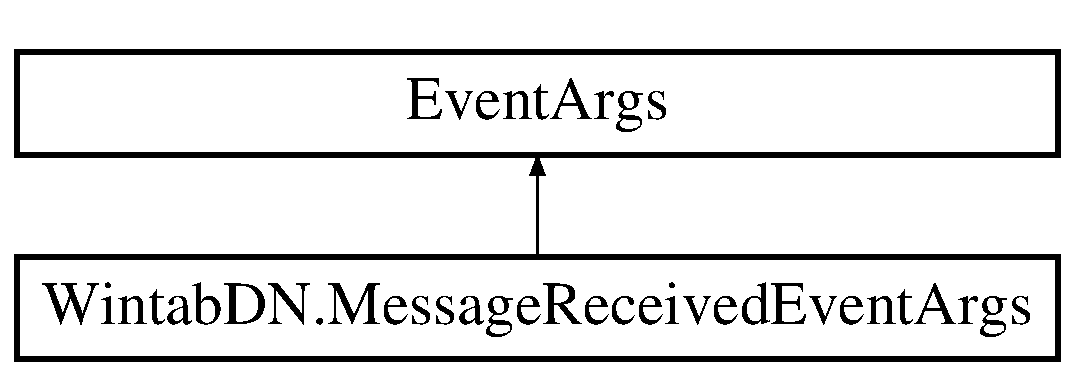
\includegraphics[height=2.000000cm]{class_wintab_d_n_1_1_message_received_event_args}
\end{center}
\end{figure}
\subsection*{Public Member Functions}
\begin{DoxyCompactItemize}
\item 
\mbox{\hyperlink{class_wintab_d_n_1_1_message_received_event_args_ae33f9fef5eac0f9a1054d846ff3ff0ab}{Message\+Received\+Event\+Args}} (\mbox{\hyperlink{class_wintab_d_n_1_1_message_received_event_args_adec3e5d29618d27908ca87ed59805b44}{Message}} message)
\begin{DoxyCompactList}\small\item\em \mbox{\hyperlink{class_wintab_d_n_1_1_message_received_event_args}{Message\+Received\+Event\+Args}} constructor. \end{DoxyCompactList}\end{DoxyCompactItemize}
\subsection*{Properties}
\begin{DoxyCompactItemize}
\item 
Message \mbox{\hyperlink{class_wintab_d_n_1_1_message_received_event_args_adec3e5d29618d27908ca87ed59805b44}{Message}}\hspace{0.3cm}{\ttfamily  \mbox{[}get\mbox{]}}
\begin{DoxyCompactList}\small\item\em Return native Windows message handled by this object. \end{DoxyCompactList}\end{DoxyCompactItemize}
\subsection*{Private Attributes}
\begin{DoxyCompactItemize}
\item 
readonly \mbox{\hyperlink{class_wintab_d_n_1_1_message_received_event_args_adec3e5d29618d27908ca87ed59805b44}{Message}} \mbox{\hyperlink{class_wintab_d_n_1_1_message_received_event_args_a2cc2a78940d81ea30f41a3001f704d65}{\+\_\+message}}
\end{DoxyCompactItemize}


\subsection{Detailed Description}
Support for registering a Native Windows message with \mbox{\hyperlink{class_wintab_d_n_1_1_message_events}{Message\+Events}} class. 



\subsection{Constructor \& Destructor Documentation}
\mbox{\Hypertarget{class_wintab_d_n_1_1_message_received_event_args_ae33f9fef5eac0f9a1054d846ff3ff0ab}\label{class_wintab_d_n_1_1_message_received_event_args_ae33f9fef5eac0f9a1054d846ff3ff0ab}} 
\index{Wintab\+D\+N\+::\+Message\+Received\+Event\+Args@{Wintab\+D\+N\+::\+Message\+Received\+Event\+Args}!Message\+Received\+Event\+Args@{Message\+Received\+Event\+Args}}
\index{Message\+Received\+Event\+Args@{Message\+Received\+Event\+Args}!Wintab\+D\+N\+::\+Message\+Received\+Event\+Args@{Wintab\+D\+N\+::\+Message\+Received\+Event\+Args}}
\subsubsection{\texorpdfstring{Message\+Received\+Event\+Args()}{MessageReceivedEventArgs()}}
{\footnotesize\ttfamily Wintab\+D\+N.\+Message\+Received\+Event\+Args.\+Message\+Received\+Event\+Args (\begin{DoxyParamCaption}\item[{\mbox{\hyperlink{class_wintab_d_n_1_1_message_received_event_args_adec3e5d29618d27908ca87ed59805b44}{Message}}}]{message }\end{DoxyParamCaption})\hspace{0.3cm}{\ttfamily [inline]}}



\mbox{\hyperlink{class_wintab_d_n_1_1_message_received_event_args}{Message\+Received\+Event\+Args}} constructor. 


\begin{DoxyParams}{Parameters}
{\em message} & Native windows message to be registered.\\
\hline
\end{DoxyParams}


\subsection{Member Data Documentation}
\mbox{\Hypertarget{class_wintab_d_n_1_1_message_received_event_args_a2cc2a78940d81ea30f41a3001f704d65}\label{class_wintab_d_n_1_1_message_received_event_args_a2cc2a78940d81ea30f41a3001f704d65}} 
\index{Wintab\+D\+N\+::\+Message\+Received\+Event\+Args@{Wintab\+D\+N\+::\+Message\+Received\+Event\+Args}!\+\_\+message@{\+\_\+message}}
\index{\+\_\+message@{\+\_\+message}!Wintab\+D\+N\+::\+Message\+Received\+Event\+Args@{Wintab\+D\+N\+::\+Message\+Received\+Event\+Args}}
\subsubsection{\texorpdfstring{\+\_\+message}{\_message}}
{\footnotesize\ttfamily readonly \mbox{\hyperlink{class_wintab_d_n_1_1_message_received_event_args_adec3e5d29618d27908ca87ed59805b44}{Message}} Wintab\+D\+N.\+Message\+Received\+Event\+Args.\+\_\+message\hspace{0.3cm}{\ttfamily [private]}}



\subsection{Property Documentation}
\mbox{\Hypertarget{class_wintab_d_n_1_1_message_received_event_args_adec3e5d29618d27908ca87ed59805b44}\label{class_wintab_d_n_1_1_message_received_event_args_adec3e5d29618d27908ca87ed59805b44}} 
\index{Wintab\+D\+N\+::\+Message\+Received\+Event\+Args@{Wintab\+D\+N\+::\+Message\+Received\+Event\+Args}!Message@{Message}}
\index{Message@{Message}!Wintab\+D\+N\+::\+Message\+Received\+Event\+Args@{Wintab\+D\+N\+::\+Message\+Received\+Event\+Args}}
\subsubsection{\texorpdfstring{Message}{Message}}
{\footnotesize\ttfamily Message Wintab\+D\+N.\+Message\+Received\+Event\+Args.\+Message\hspace{0.3cm}{\ttfamily [get]}}



Return native Windows message handled by this object. 



The documentation for this class was generated from the following file\+:\begin{DoxyCompactItemize}
\item 
Wintab\+D\+N/\mbox{\hyperlink{_message_events_8cs}{Message\+Events.\+cs}}\end{DoxyCompactItemize}

\hypertarget{class_wintab_d_n_1_1_message_events_1_1_message_window}{}\section{Wintab\+D\+N.\+Message\+Events.\+Message\+Window Class Reference}
\label{class_wintab_d_n_1_1_message_events_1_1_message_window}\index{Wintab\+D\+N.\+Message\+Events.\+Message\+Window@{Wintab\+D\+N.\+Message\+Events.\+Message\+Window}}
Inheritance diagram for Wintab\+D\+N.\+Message\+Events.\+Message\+Window\+:\begin{figure}[H]
\begin{center}
\leavevmode
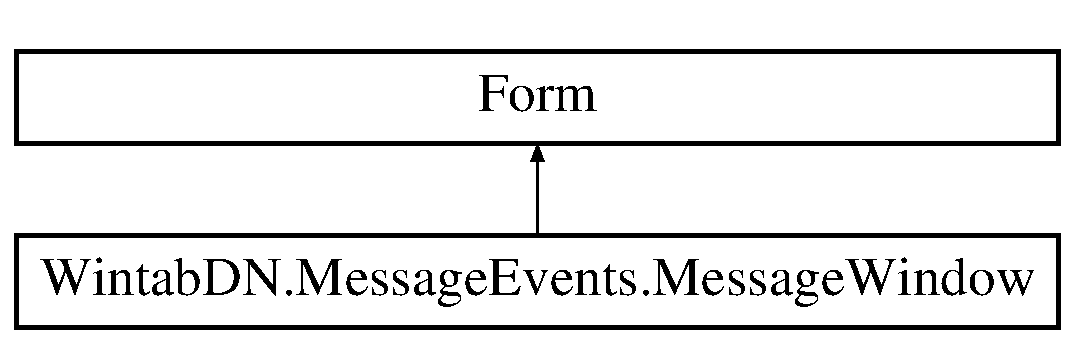
\includegraphics[height=2.000000cm]{class_wintab_d_n_1_1_message_events_1_1_message_window}
\end{center}
\end{figure}
\subsection*{Public Member Functions}
\begin{DoxyCompactItemize}
\item 
void \mbox{\hyperlink{class_wintab_d_n_1_1_message_events_1_1_message_window_af9200b16c60b75173285fa3294a02fc1}{Register\+Event\+For\+Message}} (int message\+ID)
\end{DoxyCompactItemize}
\subsection*{Protected Member Functions}
\begin{DoxyCompactItemize}
\item 
override void \mbox{\hyperlink{class_wintab_d_n_1_1_message_events_1_1_message_window_a3bd18cf029efc75766b99965e11ee62c}{Wnd\+Proc}} (ref Message m)
\end{DoxyCompactItemize}
\subsection*{Private Attributes}
\begin{DoxyCompactItemize}
\item 
Reader\+Writer\+Lock \mbox{\hyperlink{class_wintab_d_n_1_1_message_events_1_1_message_window_a7c319d57cbec3e47c834608ccda4faf6}{\+\_\+lock}} = new Reader\+Writer\+Lock()
\item 
Dictionary$<$ int, bool $>$ \mbox{\hyperlink{class_wintab_d_n_1_1_message_events_1_1_message_window_a8d2becae9e1048174dcefa03fc007019}{\+\_\+message\+Set}} = new Dictionary$<$int, bool$>$()
\end{DoxyCompactItemize}


\subsection{Member Function Documentation}
\mbox{\Hypertarget{class_wintab_d_n_1_1_message_events_1_1_message_window_af9200b16c60b75173285fa3294a02fc1}\label{class_wintab_d_n_1_1_message_events_1_1_message_window_af9200b16c60b75173285fa3294a02fc1}} 
\index{Wintab\+D\+N\+::\+Message\+Events\+::\+Message\+Window@{Wintab\+D\+N\+::\+Message\+Events\+::\+Message\+Window}!Register\+Event\+For\+Message@{Register\+Event\+For\+Message}}
\index{Register\+Event\+For\+Message@{Register\+Event\+For\+Message}!Wintab\+D\+N\+::\+Message\+Events\+::\+Message\+Window@{Wintab\+D\+N\+::\+Message\+Events\+::\+Message\+Window}}
\subsubsection{\texorpdfstring{Register\+Event\+For\+Message()}{RegisterEventForMessage()}}
{\footnotesize\ttfamily void Wintab\+D\+N.\+Message\+Events.\+Message\+Window.\+Register\+Event\+For\+Message (\begin{DoxyParamCaption}\item[{int}]{message\+ID }\end{DoxyParamCaption})\hspace{0.3cm}{\ttfamily [inline]}}

\mbox{\Hypertarget{class_wintab_d_n_1_1_message_events_1_1_message_window_a3bd18cf029efc75766b99965e11ee62c}\label{class_wintab_d_n_1_1_message_events_1_1_message_window_a3bd18cf029efc75766b99965e11ee62c}} 
\index{Wintab\+D\+N\+::\+Message\+Events\+::\+Message\+Window@{Wintab\+D\+N\+::\+Message\+Events\+::\+Message\+Window}!Wnd\+Proc@{Wnd\+Proc}}
\index{Wnd\+Proc@{Wnd\+Proc}!Wintab\+D\+N\+::\+Message\+Events\+::\+Message\+Window@{Wintab\+D\+N\+::\+Message\+Events\+::\+Message\+Window}}
\subsubsection{\texorpdfstring{Wnd\+Proc()}{WndProc()}}
{\footnotesize\ttfamily override void Wintab\+D\+N.\+Message\+Events.\+Message\+Window.\+Wnd\+Proc (\begin{DoxyParamCaption}\item[{ref Message}]{m }\end{DoxyParamCaption})\hspace{0.3cm}{\ttfamily [inline]}, {\ttfamily [protected]}}



\subsection{Member Data Documentation}
\mbox{\Hypertarget{class_wintab_d_n_1_1_message_events_1_1_message_window_a7c319d57cbec3e47c834608ccda4faf6}\label{class_wintab_d_n_1_1_message_events_1_1_message_window_a7c319d57cbec3e47c834608ccda4faf6}} 
\index{Wintab\+D\+N\+::\+Message\+Events\+::\+Message\+Window@{Wintab\+D\+N\+::\+Message\+Events\+::\+Message\+Window}!\+\_\+lock@{\+\_\+lock}}
\index{\+\_\+lock@{\+\_\+lock}!Wintab\+D\+N\+::\+Message\+Events\+::\+Message\+Window@{Wintab\+D\+N\+::\+Message\+Events\+::\+Message\+Window}}
\subsubsection{\texorpdfstring{\+\_\+lock}{\_lock}}
{\footnotesize\ttfamily Reader\+Writer\+Lock Wintab\+D\+N.\+Message\+Events.\+Message\+Window.\+\_\+lock = new Reader\+Writer\+Lock()\hspace{0.3cm}{\ttfamily [private]}}

\mbox{\Hypertarget{class_wintab_d_n_1_1_message_events_1_1_message_window_a8d2becae9e1048174dcefa03fc007019}\label{class_wintab_d_n_1_1_message_events_1_1_message_window_a8d2becae9e1048174dcefa03fc007019}} 
\index{Wintab\+D\+N\+::\+Message\+Events\+::\+Message\+Window@{Wintab\+D\+N\+::\+Message\+Events\+::\+Message\+Window}!\+\_\+message\+Set@{\+\_\+message\+Set}}
\index{\+\_\+message\+Set@{\+\_\+message\+Set}!Wintab\+D\+N\+::\+Message\+Events\+::\+Message\+Window@{Wintab\+D\+N\+::\+Message\+Events\+::\+Message\+Window}}
\subsubsection{\texorpdfstring{\+\_\+message\+Set}{\_messageSet}}
{\footnotesize\ttfamily Dictionary$<$int, bool$>$ Wintab\+D\+N.\+Message\+Events.\+Message\+Window.\+\_\+message\+Set = new Dictionary$<$int, bool$>$()\hspace{0.3cm}{\ttfamily [private]}}



The documentation for this class was generated from the following file\+:\begin{DoxyCompactItemize}
\item 
Wintab\+D\+N/\mbox{\hyperlink{_message_events_8cs}{Message\+Events.\+cs}}\end{DoxyCompactItemize}

\hypertarget{class_paint___program_1_1_move_tool}{}\section{Paint\+\_\+\+Program.\+Move\+Tool Class Reference}
\label{class_paint___program_1_1_move_tool}\index{Paint\+\_\+\+Program.\+Move\+Tool@{Paint\+\_\+\+Program.\+Move\+Tool}}
Inheritance diagram for Paint\+\_\+\+Program.\+Move\+Tool\+:\begin{figure}[H]
\begin{center}
\leavevmode
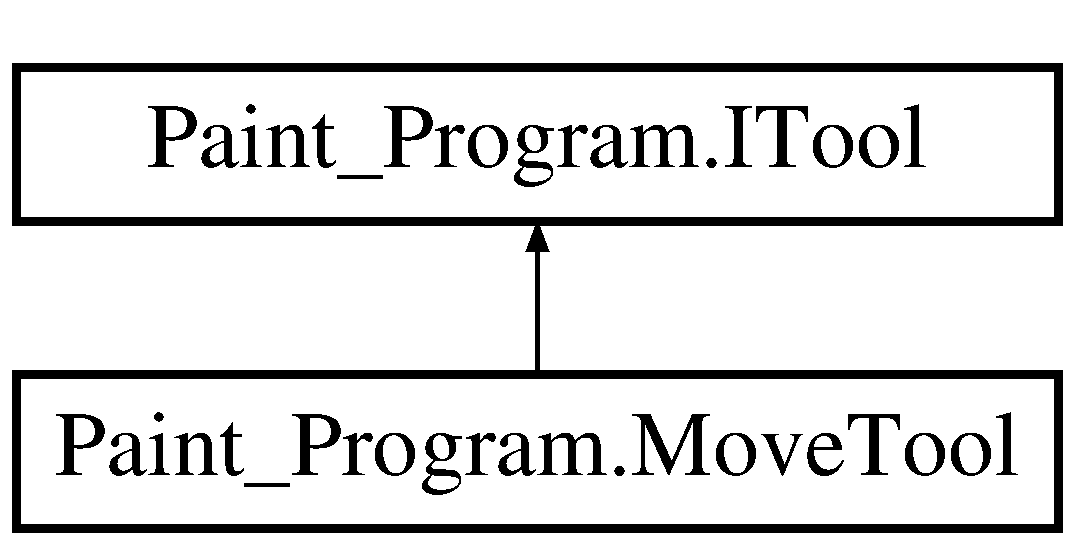
\includegraphics[height=2.000000cm]{class_paint___program_1_1_move_tool}
\end{center}
\end{figure}
\subsection*{Public Member Functions}
\begin{DoxyCompactItemize}
\item 
\mbox{\hyperlink{class_paint___program_1_1_move_tool_a42aa998e030cffd3afd1de53927327d6}{Move\+Tool}} ()
\item 
void \mbox{\hyperlink{class_paint___program_1_1_move_tool_a4dd44350bc5ba897034dca53182ac3e5}{Init}} ()
\item 
string \mbox{\hyperlink{class_paint___program_1_1_move_tool_a6341409c4de402ff447db2c542cc6b5b}{Get\+Tool\+Icon\+Path}} ()
\item 
void \mbox{\hyperlink{class_paint___program_1_1_move_tool_a0dc263e08c2709e63672d545c0ac03c2}{On\+Mouse\+Down}} (object sender, Mouse\+Event\+Args e)
\item 
void \mbox{\hyperlink{class_paint___program_1_1_move_tool_ad5062cb79928744a0b394f927eb4a41d}{On\+Mouse\+Move}} (object sender, Mouse\+Event\+Args e)
\item 
void \mbox{\hyperlink{class_paint___program_1_1_move_tool_a64daa79217e1cadfa6ddc865369298ba}{On\+Mouse\+Up}} (object sender, Mouse\+Event\+Args e)
\item 
bool \mbox{\hyperlink{class_paint___program_1_1_move_tool_a0d0d62c93c2242302143c55071231054}{is\+Initalized}} ()
\item 
Bitmap \mbox{\hyperlink{class_paint___program_1_1_move_tool_a1d458ccea18d91c95d7da179fc3503e2}{Get\+Tool\+Layer}} ()
\item 
bool \mbox{\hyperlink{class_paint___program_1_1_move_tool_ad2ef8810a173274af16797143eae1d79}{Requires\+Layer\+Data}} ()
\item 
void \mbox{\hyperlink{class_paint___program_1_1_move_tool_a3347f2d4d15477e9c9822ea8660dfc7d}{Set\+Layer\+Data}} (Bitmap bit)
\item 
string \mbox{\hyperlink{class_paint___program_1_1_move_tool_a909f48c0aa28f1f5932b42dfa076200b}{Get\+Tool\+Tip}} ()
\item 
void \mbox{\hyperlink{class_paint___program_1_1_move_tool_aae2ece279f35913a1108e3c8a93996c3}{Update\+Interface\+Layer}} ()
\end{DoxyCompactItemize}
\subsection*{Private Attributes}
\begin{DoxyCompactItemize}
\item 
Graphics \mbox{\hyperlink{class_paint___program_1_1_move_tool_add8dae61206480450c2933ba49eed5f3}{graphics}}
\item 
int \mbox{\hyperlink{class_paint___program_1_1_move_tool_ac052d025ab503efc581c5ce75caa140b}{width}}
\item 
int \mbox{\hyperlink{class_paint___program_1_1_move_tool_aa3f72d1e3720c8044becf88d53760856}{height}}
\item 
bool \mbox{\hyperlink{class_paint___program_1_1_move_tool_a380491e5f65765dca01c2220b94ad8d4}{b\+Init}}
\item 
Point \mbox{\hyperlink{class_paint___program_1_1_move_tool_ad5eab9570c8179da16a6eaeb00fb904d}{p\+Old}}
\item 
Point \mbox{\hyperlink{class_paint___program_1_1_move_tool_afb776cfa6838c75c294a66f99beaddfe}{p\+New}}
\end{DoxyCompactItemize}


\subsection{Constructor \& Destructor Documentation}
\mbox{\Hypertarget{class_paint___program_1_1_move_tool_a42aa998e030cffd3afd1de53927327d6}\label{class_paint___program_1_1_move_tool_a42aa998e030cffd3afd1de53927327d6}} 
\index{Paint\+\_\+\+Program\+::\+Move\+Tool@{Paint\+\_\+\+Program\+::\+Move\+Tool}!Move\+Tool@{Move\+Tool}}
\index{Move\+Tool@{Move\+Tool}!Paint\+\_\+\+Program\+::\+Move\+Tool@{Paint\+\_\+\+Program\+::\+Move\+Tool}}
\subsubsection{\texorpdfstring{Move\+Tool()}{MoveTool()}}
{\footnotesize\ttfamily Paint\+\_\+\+Program.\+Move\+Tool.\+Move\+Tool (\begin{DoxyParamCaption}{ }\end{DoxyParamCaption})\hspace{0.3cm}{\ttfamily [inline]}}



\subsection{Member Function Documentation}
\mbox{\Hypertarget{class_paint___program_1_1_move_tool_a6341409c4de402ff447db2c542cc6b5b}\label{class_paint___program_1_1_move_tool_a6341409c4de402ff447db2c542cc6b5b}} 
\index{Paint\+\_\+\+Program\+::\+Move\+Tool@{Paint\+\_\+\+Program\+::\+Move\+Tool}!Get\+Tool\+Icon\+Path@{Get\+Tool\+Icon\+Path}}
\index{Get\+Tool\+Icon\+Path@{Get\+Tool\+Icon\+Path}!Paint\+\_\+\+Program\+::\+Move\+Tool@{Paint\+\_\+\+Program\+::\+Move\+Tool}}
\subsubsection{\texorpdfstring{Get\+Tool\+Icon\+Path()}{GetToolIconPath()}}
{\footnotesize\ttfamily string Paint\+\_\+\+Program.\+Move\+Tool.\+Get\+Tool\+Icon\+Path (\begin{DoxyParamCaption}{ }\end{DoxyParamCaption})\hspace{0.3cm}{\ttfamily [inline]}}



Implements \mbox{\hyperlink{interface_paint___program_1_1_i_tool_aa057d2f99c59d7bec0215dcad2da1b72}{Paint\+\_\+\+Program.\+I\+Tool}}.

\mbox{\Hypertarget{class_paint___program_1_1_move_tool_a1d458ccea18d91c95d7da179fc3503e2}\label{class_paint___program_1_1_move_tool_a1d458ccea18d91c95d7da179fc3503e2}} 
\index{Paint\+\_\+\+Program\+::\+Move\+Tool@{Paint\+\_\+\+Program\+::\+Move\+Tool}!Get\+Tool\+Layer@{Get\+Tool\+Layer}}
\index{Get\+Tool\+Layer@{Get\+Tool\+Layer}!Paint\+\_\+\+Program\+::\+Move\+Tool@{Paint\+\_\+\+Program\+::\+Move\+Tool}}
\subsubsection{\texorpdfstring{Get\+Tool\+Layer()}{GetToolLayer()}}
{\footnotesize\ttfamily Bitmap Paint\+\_\+\+Program.\+Move\+Tool.\+Get\+Tool\+Layer (\begin{DoxyParamCaption}{ }\end{DoxyParamCaption})\hspace{0.3cm}{\ttfamily [inline]}}



Implements \mbox{\hyperlink{interface_paint___program_1_1_i_tool_a9b057905515f42a988c166a6a40318e0}{Paint\+\_\+\+Program.\+I\+Tool}}.

\mbox{\Hypertarget{class_paint___program_1_1_move_tool_a909f48c0aa28f1f5932b42dfa076200b}\label{class_paint___program_1_1_move_tool_a909f48c0aa28f1f5932b42dfa076200b}} 
\index{Paint\+\_\+\+Program\+::\+Move\+Tool@{Paint\+\_\+\+Program\+::\+Move\+Tool}!Get\+Tool\+Tip@{Get\+Tool\+Tip}}
\index{Get\+Tool\+Tip@{Get\+Tool\+Tip}!Paint\+\_\+\+Program\+::\+Move\+Tool@{Paint\+\_\+\+Program\+::\+Move\+Tool}}
\subsubsection{\texorpdfstring{Get\+Tool\+Tip()}{GetToolTip()}}
{\footnotesize\ttfamily string Paint\+\_\+\+Program.\+Move\+Tool.\+Get\+Tool\+Tip (\begin{DoxyParamCaption}{ }\end{DoxyParamCaption})\hspace{0.3cm}{\ttfamily [inline]}}



Implements \mbox{\hyperlink{interface_paint___program_1_1_i_tool_ac11f1591587144b6e74f5767bbf1df56}{Paint\+\_\+\+Program.\+I\+Tool}}.

\mbox{\Hypertarget{class_paint___program_1_1_move_tool_a4dd44350bc5ba897034dca53182ac3e5}\label{class_paint___program_1_1_move_tool_a4dd44350bc5ba897034dca53182ac3e5}} 
\index{Paint\+\_\+\+Program\+::\+Move\+Tool@{Paint\+\_\+\+Program\+::\+Move\+Tool}!Init@{Init}}
\index{Init@{Init}!Paint\+\_\+\+Program\+::\+Move\+Tool@{Paint\+\_\+\+Program\+::\+Move\+Tool}}
\subsubsection{\texorpdfstring{Init()}{Init()}}
{\footnotesize\ttfamily void Paint\+\_\+\+Program.\+Move\+Tool.\+Init (\begin{DoxyParamCaption}{ }\end{DoxyParamCaption})\hspace{0.3cm}{\ttfamily [inline]}}



Implements \mbox{\hyperlink{interface_paint___program_1_1_i_tool_af823123a30fbda34e24e907243241046}{Paint\+\_\+\+Program.\+I\+Tool}}.

\mbox{\Hypertarget{class_paint___program_1_1_move_tool_a0d0d62c93c2242302143c55071231054}\label{class_paint___program_1_1_move_tool_a0d0d62c93c2242302143c55071231054}} 
\index{Paint\+\_\+\+Program\+::\+Move\+Tool@{Paint\+\_\+\+Program\+::\+Move\+Tool}!is\+Initalized@{is\+Initalized}}
\index{is\+Initalized@{is\+Initalized}!Paint\+\_\+\+Program\+::\+Move\+Tool@{Paint\+\_\+\+Program\+::\+Move\+Tool}}
\subsubsection{\texorpdfstring{is\+Initalized()}{isInitalized()}}
{\footnotesize\ttfamily bool Paint\+\_\+\+Program.\+Move\+Tool.\+is\+Initalized (\begin{DoxyParamCaption}{ }\end{DoxyParamCaption})\hspace{0.3cm}{\ttfamily [inline]}}



Implements \mbox{\hyperlink{interface_paint___program_1_1_i_tool_a951b844bcbf47a6c306104fa86be7a5d}{Paint\+\_\+\+Program.\+I\+Tool}}.

\mbox{\Hypertarget{class_paint___program_1_1_move_tool_a0dc263e08c2709e63672d545c0ac03c2}\label{class_paint___program_1_1_move_tool_a0dc263e08c2709e63672d545c0ac03c2}} 
\index{Paint\+\_\+\+Program\+::\+Move\+Tool@{Paint\+\_\+\+Program\+::\+Move\+Tool}!On\+Mouse\+Down@{On\+Mouse\+Down}}
\index{On\+Mouse\+Down@{On\+Mouse\+Down}!Paint\+\_\+\+Program\+::\+Move\+Tool@{Paint\+\_\+\+Program\+::\+Move\+Tool}}
\subsubsection{\texorpdfstring{On\+Mouse\+Down()}{OnMouseDown()}}
{\footnotesize\ttfamily void Paint\+\_\+\+Program.\+Move\+Tool.\+On\+Mouse\+Down (\begin{DoxyParamCaption}\item[{object}]{sender,  }\item[{Mouse\+Event\+Args}]{e }\end{DoxyParamCaption})\hspace{0.3cm}{\ttfamily [inline]}}



Implements \mbox{\hyperlink{interface_paint___program_1_1_i_tool_a73d8797f4f2b1e0d8efe8aadcd44e840}{Paint\+\_\+\+Program.\+I\+Tool}}.

\mbox{\Hypertarget{class_paint___program_1_1_move_tool_ad5062cb79928744a0b394f927eb4a41d}\label{class_paint___program_1_1_move_tool_ad5062cb79928744a0b394f927eb4a41d}} 
\index{Paint\+\_\+\+Program\+::\+Move\+Tool@{Paint\+\_\+\+Program\+::\+Move\+Tool}!On\+Mouse\+Move@{On\+Mouse\+Move}}
\index{On\+Mouse\+Move@{On\+Mouse\+Move}!Paint\+\_\+\+Program\+::\+Move\+Tool@{Paint\+\_\+\+Program\+::\+Move\+Tool}}
\subsubsection{\texorpdfstring{On\+Mouse\+Move()}{OnMouseMove()}}
{\footnotesize\ttfamily void Paint\+\_\+\+Program.\+Move\+Tool.\+On\+Mouse\+Move (\begin{DoxyParamCaption}\item[{object}]{sender,  }\item[{Mouse\+Event\+Args}]{e }\end{DoxyParamCaption})\hspace{0.3cm}{\ttfamily [inline]}}



Implements \mbox{\hyperlink{interface_paint___program_1_1_i_tool_a6a1cbe840b5cfc8a9b9463cc21590845}{Paint\+\_\+\+Program.\+I\+Tool}}.

\mbox{\Hypertarget{class_paint___program_1_1_move_tool_a64daa79217e1cadfa6ddc865369298ba}\label{class_paint___program_1_1_move_tool_a64daa79217e1cadfa6ddc865369298ba}} 
\index{Paint\+\_\+\+Program\+::\+Move\+Tool@{Paint\+\_\+\+Program\+::\+Move\+Tool}!On\+Mouse\+Up@{On\+Mouse\+Up}}
\index{On\+Mouse\+Up@{On\+Mouse\+Up}!Paint\+\_\+\+Program\+::\+Move\+Tool@{Paint\+\_\+\+Program\+::\+Move\+Tool}}
\subsubsection{\texorpdfstring{On\+Mouse\+Up()}{OnMouseUp()}}
{\footnotesize\ttfamily void Paint\+\_\+\+Program.\+Move\+Tool.\+On\+Mouse\+Up (\begin{DoxyParamCaption}\item[{object}]{sender,  }\item[{Mouse\+Event\+Args}]{e }\end{DoxyParamCaption})\hspace{0.3cm}{\ttfamily [inline]}}



Implements \mbox{\hyperlink{interface_paint___program_1_1_i_tool_a47984c2879213022f1684c07f7bba73e}{Paint\+\_\+\+Program.\+I\+Tool}}.

\mbox{\Hypertarget{class_paint___program_1_1_move_tool_ad2ef8810a173274af16797143eae1d79}\label{class_paint___program_1_1_move_tool_ad2ef8810a173274af16797143eae1d79}} 
\index{Paint\+\_\+\+Program\+::\+Move\+Tool@{Paint\+\_\+\+Program\+::\+Move\+Tool}!Requires\+Layer\+Data@{Requires\+Layer\+Data}}
\index{Requires\+Layer\+Data@{Requires\+Layer\+Data}!Paint\+\_\+\+Program\+::\+Move\+Tool@{Paint\+\_\+\+Program\+::\+Move\+Tool}}
\subsubsection{\texorpdfstring{Requires\+Layer\+Data()}{RequiresLayerData()}}
{\footnotesize\ttfamily bool Paint\+\_\+\+Program.\+Move\+Tool.\+Requires\+Layer\+Data (\begin{DoxyParamCaption}{ }\end{DoxyParamCaption})\hspace{0.3cm}{\ttfamily [inline]}}



Implements \mbox{\hyperlink{interface_paint___program_1_1_i_tool_a6d45b6c48da8130ae41db3a66cdaef9a}{Paint\+\_\+\+Program.\+I\+Tool}}.

\mbox{\Hypertarget{class_paint___program_1_1_move_tool_a3347f2d4d15477e9c9822ea8660dfc7d}\label{class_paint___program_1_1_move_tool_a3347f2d4d15477e9c9822ea8660dfc7d}} 
\index{Paint\+\_\+\+Program\+::\+Move\+Tool@{Paint\+\_\+\+Program\+::\+Move\+Tool}!Set\+Layer\+Data@{Set\+Layer\+Data}}
\index{Set\+Layer\+Data@{Set\+Layer\+Data}!Paint\+\_\+\+Program\+::\+Move\+Tool@{Paint\+\_\+\+Program\+::\+Move\+Tool}}
\subsubsection{\texorpdfstring{Set\+Layer\+Data()}{SetLayerData()}}
{\footnotesize\ttfamily void Paint\+\_\+\+Program.\+Move\+Tool.\+Set\+Layer\+Data (\begin{DoxyParamCaption}\item[{Bitmap}]{bit }\end{DoxyParamCaption})\hspace{0.3cm}{\ttfamily [inline]}}



Implements \mbox{\hyperlink{interface_paint___program_1_1_i_tool_a2d3e63715dfe04075d27dacf367d1633}{Paint\+\_\+\+Program.\+I\+Tool}}.

\mbox{\Hypertarget{class_paint___program_1_1_move_tool_aae2ece279f35913a1108e3c8a93996c3}\label{class_paint___program_1_1_move_tool_aae2ece279f35913a1108e3c8a93996c3}} 
\index{Paint\+\_\+\+Program\+::\+Move\+Tool@{Paint\+\_\+\+Program\+::\+Move\+Tool}!Update\+Interface\+Layer@{Update\+Interface\+Layer}}
\index{Update\+Interface\+Layer@{Update\+Interface\+Layer}!Paint\+\_\+\+Program\+::\+Move\+Tool@{Paint\+\_\+\+Program\+::\+Move\+Tool}}
\subsubsection{\texorpdfstring{Update\+Interface\+Layer()}{UpdateInterfaceLayer()}}
{\footnotesize\ttfamily void Paint\+\_\+\+Program.\+Move\+Tool.\+Update\+Interface\+Layer (\begin{DoxyParamCaption}{ }\end{DoxyParamCaption})\hspace{0.3cm}{\ttfamily [inline]}}



Implements \mbox{\hyperlink{interface_paint___program_1_1_i_tool_a36db75d29e88dfd739f658633c40e955}{Paint\+\_\+\+Program.\+I\+Tool}}.



\subsection{Member Data Documentation}
\mbox{\Hypertarget{class_paint___program_1_1_move_tool_a380491e5f65765dca01c2220b94ad8d4}\label{class_paint___program_1_1_move_tool_a380491e5f65765dca01c2220b94ad8d4}} 
\index{Paint\+\_\+\+Program\+::\+Move\+Tool@{Paint\+\_\+\+Program\+::\+Move\+Tool}!b\+Init@{b\+Init}}
\index{b\+Init@{b\+Init}!Paint\+\_\+\+Program\+::\+Move\+Tool@{Paint\+\_\+\+Program\+::\+Move\+Tool}}
\subsubsection{\texorpdfstring{b\+Init}{bInit}}
{\footnotesize\ttfamily bool Paint\+\_\+\+Program.\+Move\+Tool.\+b\+Init\hspace{0.3cm}{\ttfamily [private]}}

\mbox{\Hypertarget{class_paint___program_1_1_move_tool_add8dae61206480450c2933ba49eed5f3}\label{class_paint___program_1_1_move_tool_add8dae61206480450c2933ba49eed5f3}} 
\index{Paint\+\_\+\+Program\+::\+Move\+Tool@{Paint\+\_\+\+Program\+::\+Move\+Tool}!graphics@{graphics}}
\index{graphics@{graphics}!Paint\+\_\+\+Program\+::\+Move\+Tool@{Paint\+\_\+\+Program\+::\+Move\+Tool}}
\subsubsection{\texorpdfstring{graphics}{graphics}}
{\footnotesize\ttfamily Graphics Paint\+\_\+\+Program.\+Move\+Tool.\+graphics\hspace{0.3cm}{\ttfamily [private]}}

\mbox{\Hypertarget{class_paint___program_1_1_move_tool_aa3f72d1e3720c8044becf88d53760856}\label{class_paint___program_1_1_move_tool_aa3f72d1e3720c8044becf88d53760856}} 
\index{Paint\+\_\+\+Program\+::\+Move\+Tool@{Paint\+\_\+\+Program\+::\+Move\+Tool}!height@{height}}
\index{height@{height}!Paint\+\_\+\+Program\+::\+Move\+Tool@{Paint\+\_\+\+Program\+::\+Move\+Tool}}
\subsubsection{\texorpdfstring{height}{height}}
{\footnotesize\ttfamily int Paint\+\_\+\+Program.\+Move\+Tool.\+height\hspace{0.3cm}{\ttfamily [private]}}

\mbox{\Hypertarget{class_paint___program_1_1_move_tool_afb776cfa6838c75c294a66f99beaddfe}\label{class_paint___program_1_1_move_tool_afb776cfa6838c75c294a66f99beaddfe}} 
\index{Paint\+\_\+\+Program\+::\+Move\+Tool@{Paint\+\_\+\+Program\+::\+Move\+Tool}!p\+New@{p\+New}}
\index{p\+New@{p\+New}!Paint\+\_\+\+Program\+::\+Move\+Tool@{Paint\+\_\+\+Program\+::\+Move\+Tool}}
\subsubsection{\texorpdfstring{p\+New}{pNew}}
{\footnotesize\ttfamily Point Paint\+\_\+\+Program.\+Move\+Tool.\+p\+New\hspace{0.3cm}{\ttfamily [private]}}

\mbox{\Hypertarget{class_paint___program_1_1_move_tool_ad5eab9570c8179da16a6eaeb00fb904d}\label{class_paint___program_1_1_move_tool_ad5eab9570c8179da16a6eaeb00fb904d}} 
\index{Paint\+\_\+\+Program\+::\+Move\+Tool@{Paint\+\_\+\+Program\+::\+Move\+Tool}!p\+Old@{p\+Old}}
\index{p\+Old@{p\+Old}!Paint\+\_\+\+Program\+::\+Move\+Tool@{Paint\+\_\+\+Program\+::\+Move\+Tool}}
\subsubsection{\texorpdfstring{p\+Old}{pOld}}
{\footnotesize\ttfamily Point Paint\+\_\+\+Program.\+Move\+Tool.\+p\+Old\hspace{0.3cm}{\ttfamily [private]}}

\mbox{\Hypertarget{class_paint___program_1_1_move_tool_ac052d025ab503efc581c5ce75caa140b}\label{class_paint___program_1_1_move_tool_ac052d025ab503efc581c5ce75caa140b}} 
\index{Paint\+\_\+\+Program\+::\+Move\+Tool@{Paint\+\_\+\+Program\+::\+Move\+Tool}!width@{width}}
\index{width@{width}!Paint\+\_\+\+Program\+::\+Move\+Tool@{Paint\+\_\+\+Program\+::\+Move\+Tool}}
\subsubsection{\texorpdfstring{width}{width}}
{\footnotesize\ttfamily int Paint\+\_\+\+Program.\+Move\+Tool.\+width\hspace{0.3cm}{\ttfamily [private]}}



The documentation for this class was generated from the following file\+:\begin{DoxyCompactItemize}
\item 
Paint Program/\mbox{\hyperlink{_move_tool_8cs}{Move\+Tool.\+cs}}\end{DoxyCompactItemize}

\hypertarget{class_paint___program_1_1_new_project_form}{}\section{Paint\+\_\+\+Program.\+New\+Project\+Form Class Reference}
\label{class_paint___program_1_1_new_project_form}\index{Paint\+\_\+\+Program.\+New\+Project\+Form@{Paint\+\_\+\+Program.\+New\+Project\+Form}}
Inheritance diagram for Paint\+\_\+\+Program.\+New\+Project\+Form\+:\begin{figure}[H]
\begin{center}
\leavevmode
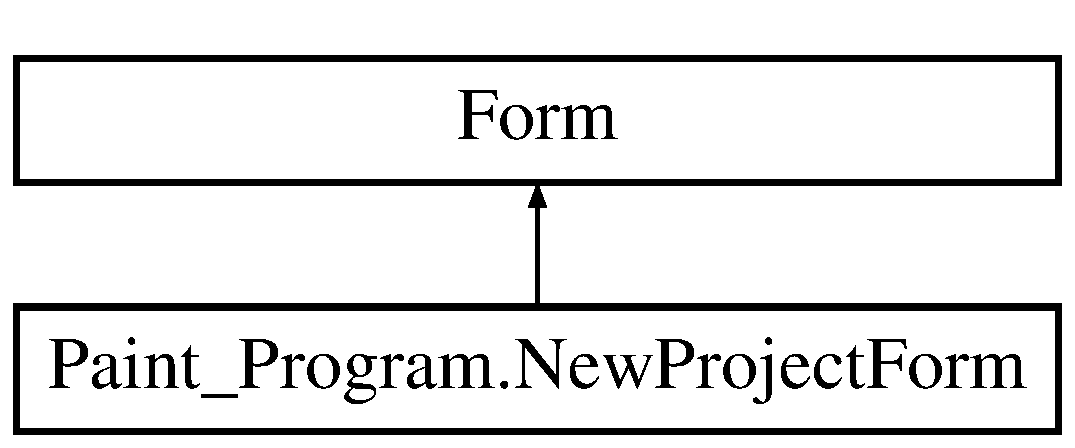
\includegraphics[height=2.000000cm]{class_paint___program_1_1_new_project_form}
\end{center}
\end{figure}
\subsection*{Public Member Functions}
\begin{DoxyCompactItemize}
\item 
\mbox{\hyperlink{class_paint___program_1_1_new_project_form_a9d6022141bf286fea16115218f1f16ea}{New\+Project\+Form}} ()
\end{DoxyCompactItemize}
\subsection*{Protected Member Functions}
\begin{DoxyCompactItemize}
\item 
override void \mbox{\hyperlink{class_paint___program_1_1_new_project_form_a48d91b7fc622b68f9c6a665051a4548f}{Dispose}} (bool disposing)
\begin{DoxyCompactList}\small\item\em Clean up any resources being used. \end{DoxyCompactList}\end{DoxyCompactItemize}
\subsection*{Properties}
\begin{DoxyCompactItemize}
\item 
int \mbox{\hyperlink{class_paint___program_1_1_new_project_form_a60a41bc537a843dacb79c67b4cc6ac5f}{Canvas\+Width}}\hspace{0.3cm}{\ttfamily  \mbox{[}get, private set\mbox{]}}
\item 
int \mbox{\hyperlink{class_paint___program_1_1_new_project_form_a14997bfb0df33e50fc9125b8cfd25238}{Canvas\+Height}}\hspace{0.3cm}{\ttfamily  \mbox{[}get, private set\mbox{]}}
\end{DoxyCompactItemize}
\subsection*{Private Member Functions}
\begin{DoxyCompactItemize}
\item 
void \mbox{\hyperlink{class_paint___program_1_1_new_project_form_aa43d720d3ebb5f1dbb1ee6dcc2c714c8}{b\+Submit\+\_\+\+Click}} (object sender, Event\+Args e)
\item 
void \mbox{\hyperlink{class_paint___program_1_1_new_project_form_a04b3a294a9113ed06ecfa74192e42958}{Handle\+\_\+\+Key\+Press}} (object sender, Key\+Event\+Args e)
\item 
void \mbox{\hyperlink{class_paint___program_1_1_new_project_form_ae85795537ab7ad2b2bf2775510e260ba}{Initialize\+Component}} ()
\begin{DoxyCompactList}\small\item\em Required method for Designer support -\/ do not modify the contents of this method with the code editor. \end{DoxyCompactList}\end{DoxyCompactItemize}
\subsection*{Private Attributes}
\begin{DoxyCompactItemize}
\item 
System.\+Component\+Model.\+I\+Container \mbox{\hyperlink{class_paint___program_1_1_new_project_form_abac36a8b7050e7b6024c69bff809c5c0}{components}} = null
\begin{DoxyCompactList}\small\item\em Required designer variable. \end{DoxyCompactList}\item 
System.\+Windows.\+Forms.\+Label \mbox{\hyperlink{class_paint___program_1_1_new_project_form_ae759110ede1404912e21e9385f6a4572}{l\+Width}}
\item 
System.\+Windows.\+Forms.\+Label \mbox{\hyperlink{class_paint___program_1_1_new_project_form_a1154f326067af764865f0c82efee2992}{l\+Height}}
\item 
System.\+Windows.\+Forms.\+Text\+Box \mbox{\hyperlink{class_paint___program_1_1_new_project_form_a56fe3a72511892792928d3f350a2835f}{tb\+Width}}
\item 
System.\+Windows.\+Forms.\+Text\+Box \mbox{\hyperlink{class_paint___program_1_1_new_project_form_a27613df56889f1978b5c3fbed6aea1ee}{tb\+Height}}
\item 
System.\+Windows.\+Forms.\+Button \mbox{\hyperlink{class_paint___program_1_1_new_project_form_a7601a0b6fc14d0b1ec52e98cd492cfda}{b\+Submit}}
\end{DoxyCompactItemize}


\subsection{Constructor \& Destructor Documentation}
\mbox{\Hypertarget{class_paint___program_1_1_new_project_form_a9d6022141bf286fea16115218f1f16ea}\label{class_paint___program_1_1_new_project_form_a9d6022141bf286fea16115218f1f16ea}} 
\index{Paint\+\_\+\+Program\+::\+New\+Project\+Form@{Paint\+\_\+\+Program\+::\+New\+Project\+Form}!New\+Project\+Form@{New\+Project\+Form}}
\index{New\+Project\+Form@{New\+Project\+Form}!Paint\+\_\+\+Program\+::\+New\+Project\+Form@{Paint\+\_\+\+Program\+::\+New\+Project\+Form}}
\subsubsection{\texorpdfstring{New\+Project\+Form()}{NewProjectForm()}}
{\footnotesize\ttfamily Paint\+\_\+\+Program.\+New\+Project\+Form.\+New\+Project\+Form (\begin{DoxyParamCaption}{ }\end{DoxyParamCaption})\hspace{0.3cm}{\ttfamily [inline]}}



\subsection{Member Function Documentation}
\mbox{\Hypertarget{class_paint___program_1_1_new_project_form_aa43d720d3ebb5f1dbb1ee6dcc2c714c8}\label{class_paint___program_1_1_new_project_form_aa43d720d3ebb5f1dbb1ee6dcc2c714c8}} 
\index{Paint\+\_\+\+Program\+::\+New\+Project\+Form@{Paint\+\_\+\+Program\+::\+New\+Project\+Form}!b\+Submit\+\_\+\+Click@{b\+Submit\+\_\+\+Click}}
\index{b\+Submit\+\_\+\+Click@{b\+Submit\+\_\+\+Click}!Paint\+\_\+\+Program\+::\+New\+Project\+Form@{Paint\+\_\+\+Program\+::\+New\+Project\+Form}}
\subsubsection{\texorpdfstring{b\+Submit\+\_\+\+Click()}{bSubmit\_Click()}}
{\footnotesize\ttfamily void Paint\+\_\+\+Program.\+New\+Project\+Form.\+b\+Submit\+\_\+\+Click (\begin{DoxyParamCaption}\item[{object}]{sender,  }\item[{Event\+Args}]{e }\end{DoxyParamCaption})\hspace{0.3cm}{\ttfamily [inline]}, {\ttfamily [private]}}

\mbox{\Hypertarget{class_paint___program_1_1_new_project_form_a48d91b7fc622b68f9c6a665051a4548f}\label{class_paint___program_1_1_new_project_form_a48d91b7fc622b68f9c6a665051a4548f}} 
\index{Paint\+\_\+\+Program\+::\+New\+Project\+Form@{Paint\+\_\+\+Program\+::\+New\+Project\+Form}!Dispose@{Dispose}}
\index{Dispose@{Dispose}!Paint\+\_\+\+Program\+::\+New\+Project\+Form@{Paint\+\_\+\+Program\+::\+New\+Project\+Form}}
\subsubsection{\texorpdfstring{Dispose()}{Dispose()}}
{\footnotesize\ttfamily override void Paint\+\_\+\+Program.\+New\+Project\+Form.\+Dispose (\begin{DoxyParamCaption}\item[{bool}]{disposing }\end{DoxyParamCaption})\hspace{0.3cm}{\ttfamily [inline]}, {\ttfamily [protected]}}



Clean up any resources being used. 


\begin{DoxyParams}{Parameters}
{\em disposing} & true if managed resources should be disposed; otherwise, false.\\
\hline
\end{DoxyParams}
\mbox{\Hypertarget{class_paint___program_1_1_new_project_form_a04b3a294a9113ed06ecfa74192e42958}\label{class_paint___program_1_1_new_project_form_a04b3a294a9113ed06ecfa74192e42958}} 
\index{Paint\+\_\+\+Program\+::\+New\+Project\+Form@{Paint\+\_\+\+Program\+::\+New\+Project\+Form}!Handle\+\_\+\+Key\+Press@{Handle\+\_\+\+Key\+Press}}
\index{Handle\+\_\+\+Key\+Press@{Handle\+\_\+\+Key\+Press}!Paint\+\_\+\+Program\+::\+New\+Project\+Form@{Paint\+\_\+\+Program\+::\+New\+Project\+Form}}
\subsubsection{\texorpdfstring{Handle\+\_\+\+Key\+Press()}{Handle\_KeyPress()}}
{\footnotesize\ttfamily void Paint\+\_\+\+Program.\+New\+Project\+Form.\+Handle\+\_\+\+Key\+Press (\begin{DoxyParamCaption}\item[{object}]{sender,  }\item[{Key\+Event\+Args}]{e }\end{DoxyParamCaption})\hspace{0.3cm}{\ttfamily [inline]}, {\ttfamily [private]}}

\mbox{\Hypertarget{class_paint___program_1_1_new_project_form_ae85795537ab7ad2b2bf2775510e260ba}\label{class_paint___program_1_1_new_project_form_ae85795537ab7ad2b2bf2775510e260ba}} 
\index{Paint\+\_\+\+Program\+::\+New\+Project\+Form@{Paint\+\_\+\+Program\+::\+New\+Project\+Form}!Initialize\+Component@{Initialize\+Component}}
\index{Initialize\+Component@{Initialize\+Component}!Paint\+\_\+\+Program\+::\+New\+Project\+Form@{Paint\+\_\+\+Program\+::\+New\+Project\+Form}}
\subsubsection{\texorpdfstring{Initialize\+Component()}{InitializeComponent()}}
{\footnotesize\ttfamily void Paint\+\_\+\+Program.\+New\+Project\+Form.\+Initialize\+Component (\begin{DoxyParamCaption}{ }\end{DoxyParamCaption})\hspace{0.3cm}{\ttfamily [inline]}, {\ttfamily [private]}}



Required method for Designer support -\/ do not modify the contents of this method with the code editor. 



\subsection{Member Data Documentation}
\mbox{\Hypertarget{class_paint___program_1_1_new_project_form_a7601a0b6fc14d0b1ec52e98cd492cfda}\label{class_paint___program_1_1_new_project_form_a7601a0b6fc14d0b1ec52e98cd492cfda}} 
\index{Paint\+\_\+\+Program\+::\+New\+Project\+Form@{Paint\+\_\+\+Program\+::\+New\+Project\+Form}!b\+Submit@{b\+Submit}}
\index{b\+Submit@{b\+Submit}!Paint\+\_\+\+Program\+::\+New\+Project\+Form@{Paint\+\_\+\+Program\+::\+New\+Project\+Form}}
\subsubsection{\texorpdfstring{b\+Submit}{bSubmit}}
{\footnotesize\ttfamily System.\+Windows.\+Forms.\+Button Paint\+\_\+\+Program.\+New\+Project\+Form.\+b\+Submit\hspace{0.3cm}{\ttfamily [private]}}

\mbox{\Hypertarget{class_paint___program_1_1_new_project_form_abac36a8b7050e7b6024c69bff809c5c0}\label{class_paint___program_1_1_new_project_form_abac36a8b7050e7b6024c69bff809c5c0}} 
\index{Paint\+\_\+\+Program\+::\+New\+Project\+Form@{Paint\+\_\+\+Program\+::\+New\+Project\+Form}!components@{components}}
\index{components@{components}!Paint\+\_\+\+Program\+::\+New\+Project\+Form@{Paint\+\_\+\+Program\+::\+New\+Project\+Form}}
\subsubsection{\texorpdfstring{components}{components}}
{\footnotesize\ttfamily System.\+Component\+Model.\+I\+Container Paint\+\_\+\+Program.\+New\+Project\+Form.\+components = null\hspace{0.3cm}{\ttfamily [private]}}



Required designer variable. 

\mbox{\Hypertarget{class_paint___program_1_1_new_project_form_a1154f326067af764865f0c82efee2992}\label{class_paint___program_1_1_new_project_form_a1154f326067af764865f0c82efee2992}} 
\index{Paint\+\_\+\+Program\+::\+New\+Project\+Form@{Paint\+\_\+\+Program\+::\+New\+Project\+Form}!l\+Height@{l\+Height}}
\index{l\+Height@{l\+Height}!Paint\+\_\+\+Program\+::\+New\+Project\+Form@{Paint\+\_\+\+Program\+::\+New\+Project\+Form}}
\subsubsection{\texorpdfstring{l\+Height}{lHeight}}
{\footnotesize\ttfamily System.\+Windows.\+Forms.\+Label Paint\+\_\+\+Program.\+New\+Project\+Form.\+l\+Height\hspace{0.3cm}{\ttfamily [private]}}

\mbox{\Hypertarget{class_paint___program_1_1_new_project_form_ae759110ede1404912e21e9385f6a4572}\label{class_paint___program_1_1_new_project_form_ae759110ede1404912e21e9385f6a4572}} 
\index{Paint\+\_\+\+Program\+::\+New\+Project\+Form@{Paint\+\_\+\+Program\+::\+New\+Project\+Form}!l\+Width@{l\+Width}}
\index{l\+Width@{l\+Width}!Paint\+\_\+\+Program\+::\+New\+Project\+Form@{Paint\+\_\+\+Program\+::\+New\+Project\+Form}}
\subsubsection{\texorpdfstring{l\+Width}{lWidth}}
{\footnotesize\ttfamily System.\+Windows.\+Forms.\+Label Paint\+\_\+\+Program.\+New\+Project\+Form.\+l\+Width\hspace{0.3cm}{\ttfamily [private]}}

\mbox{\Hypertarget{class_paint___program_1_1_new_project_form_a27613df56889f1978b5c3fbed6aea1ee}\label{class_paint___program_1_1_new_project_form_a27613df56889f1978b5c3fbed6aea1ee}} 
\index{Paint\+\_\+\+Program\+::\+New\+Project\+Form@{Paint\+\_\+\+Program\+::\+New\+Project\+Form}!tb\+Height@{tb\+Height}}
\index{tb\+Height@{tb\+Height}!Paint\+\_\+\+Program\+::\+New\+Project\+Form@{Paint\+\_\+\+Program\+::\+New\+Project\+Form}}
\subsubsection{\texorpdfstring{tb\+Height}{tbHeight}}
{\footnotesize\ttfamily System.\+Windows.\+Forms.\+Text\+Box Paint\+\_\+\+Program.\+New\+Project\+Form.\+tb\+Height\hspace{0.3cm}{\ttfamily [private]}}

\mbox{\Hypertarget{class_paint___program_1_1_new_project_form_a56fe3a72511892792928d3f350a2835f}\label{class_paint___program_1_1_new_project_form_a56fe3a72511892792928d3f350a2835f}} 
\index{Paint\+\_\+\+Program\+::\+New\+Project\+Form@{Paint\+\_\+\+Program\+::\+New\+Project\+Form}!tb\+Width@{tb\+Width}}
\index{tb\+Width@{tb\+Width}!Paint\+\_\+\+Program\+::\+New\+Project\+Form@{Paint\+\_\+\+Program\+::\+New\+Project\+Form}}
\subsubsection{\texorpdfstring{tb\+Width}{tbWidth}}
{\footnotesize\ttfamily System.\+Windows.\+Forms.\+Text\+Box Paint\+\_\+\+Program.\+New\+Project\+Form.\+tb\+Width\hspace{0.3cm}{\ttfamily [private]}}



\subsection{Property Documentation}
\mbox{\Hypertarget{class_paint___program_1_1_new_project_form_a14997bfb0df33e50fc9125b8cfd25238}\label{class_paint___program_1_1_new_project_form_a14997bfb0df33e50fc9125b8cfd25238}} 
\index{Paint\+\_\+\+Program\+::\+New\+Project\+Form@{Paint\+\_\+\+Program\+::\+New\+Project\+Form}!Canvas\+Height@{Canvas\+Height}}
\index{Canvas\+Height@{Canvas\+Height}!Paint\+\_\+\+Program\+::\+New\+Project\+Form@{Paint\+\_\+\+Program\+::\+New\+Project\+Form}}
\subsubsection{\texorpdfstring{Canvas\+Height}{CanvasHeight}}
{\footnotesize\ttfamily int Paint\+\_\+\+Program.\+New\+Project\+Form.\+Canvas\+Height\hspace{0.3cm}{\ttfamily [get]}, {\ttfamily [private set]}}

\mbox{\Hypertarget{class_paint___program_1_1_new_project_form_a60a41bc537a843dacb79c67b4cc6ac5f}\label{class_paint___program_1_1_new_project_form_a60a41bc537a843dacb79c67b4cc6ac5f}} 
\index{Paint\+\_\+\+Program\+::\+New\+Project\+Form@{Paint\+\_\+\+Program\+::\+New\+Project\+Form}!Canvas\+Width@{Canvas\+Width}}
\index{Canvas\+Width@{Canvas\+Width}!Paint\+\_\+\+Program\+::\+New\+Project\+Form@{Paint\+\_\+\+Program\+::\+New\+Project\+Form}}
\subsubsection{\texorpdfstring{Canvas\+Width}{CanvasWidth}}
{\footnotesize\ttfamily int Paint\+\_\+\+Program.\+New\+Project\+Form.\+Canvas\+Width\hspace{0.3cm}{\ttfamily [get]}, {\ttfamily [private set]}}



The documentation for this class was generated from the following files\+:\begin{DoxyCompactItemize}
\item 
Paint Program/\mbox{\hyperlink{_new_project_form_8cs}{New\+Project\+Form.\+cs}}\item 
Paint Program/\mbox{\hyperlink{_new_project_form_8_designer_8cs}{New\+Project\+Form.\+Designer.\+cs}}\end{DoxyCompactItemize}

\hypertarget{class_paint___program_1_1_paint_bucket_tool}{}\section{Paint\+\_\+\+Program.\+Paint\+Bucket\+Tool Class Reference}
\label{class_paint___program_1_1_paint_bucket_tool}\index{Paint\+\_\+\+Program.\+Paint\+Bucket\+Tool@{Paint\+\_\+\+Program.\+Paint\+Bucket\+Tool}}
Inheritance diagram for Paint\+\_\+\+Program.\+Paint\+Bucket\+Tool\+:\begin{figure}[H]
\begin{center}
\leavevmode
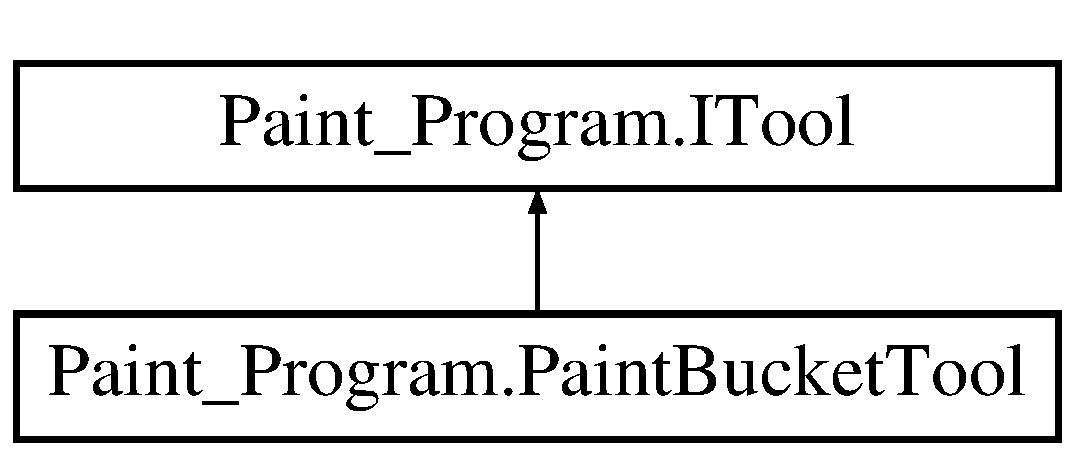
\includegraphics[height=2.000000cm]{class_paint___program_1_1_paint_bucket_tool}
\end{center}
\end{figure}
\subsection*{Public Member Functions}
\begin{DoxyCompactItemize}
\item 
bool \mbox{\hyperlink{class_paint___program_1_1_paint_bucket_tool_a897f50631adb267c4b0a5e242c9bfaa5}{Color\+Match}} (Color a, Color b)
\item 
void \mbox{\hyperlink{class_paint___program_1_1_paint_bucket_tool_a9702953f92a727585a7d12507070963e}{Add\+Next\+Pixel}} (Point p)
\item 
\mbox{\hyperlink{class_paint___program_1_1_paint_bucket_tool_acff0d603cffb8e2b068e5ab74a63c9bd}{Paint\+Bucket\+Tool}} ()
\item 
void \mbox{\hyperlink{class_paint___program_1_1_paint_bucket_tool_a2de33717bdf3555d97e5e6e962602f85}{Init}} ()
\item 
string \mbox{\hyperlink{class_paint___program_1_1_paint_bucket_tool_aef69a21dec547869dde171a604bf1492}{Get\+Tool\+Icon\+Path}} ()
\item 
void \mbox{\hyperlink{class_paint___program_1_1_paint_bucket_tool_a468286c5eb5f2a49fe92387b9c859398}{On\+Mouse\+Down}} (object sender, Mouse\+Event\+Args e)
\item 
void \mbox{\hyperlink{class_paint___program_1_1_paint_bucket_tool_a0a4dfeb323d746b531ece7d4a9e218a7}{On\+Mouse\+Move}} (object sender, Mouse\+Event\+Args e)
\item 
void \mbox{\hyperlink{class_paint___program_1_1_paint_bucket_tool_a3841a712dff7c2887a4518d7602b627e}{On\+Mouse\+Up}} (object sender, Mouse\+Event\+Args e)
\item 
bool \mbox{\hyperlink{class_paint___program_1_1_paint_bucket_tool_ad41b8e00b3715186451c6caadc595db8}{is\+Initalized}} ()
\item 
Bitmap \mbox{\hyperlink{class_paint___program_1_1_paint_bucket_tool_a3167ad9df7812f1f857e0a869a455ff6}{Get\+Tool\+Layer}} ()
\item 
bool \mbox{\hyperlink{class_paint___program_1_1_paint_bucket_tool_a634df2c5ddde570dc6c73abe5c680266}{Requires\+Layer\+Data}} ()
\item 
void \mbox{\hyperlink{class_paint___program_1_1_paint_bucket_tool_ab2716c454849a952526e94c40bba90b6}{Set\+Layer\+Data}} (Bitmap bit)
\item 
string \mbox{\hyperlink{class_paint___program_1_1_paint_bucket_tool_af890852ac2b519cc0d2a7a767e09fe2d}{Get\+Tool\+Tip}} ()
\item 
void \mbox{\hyperlink{class_paint___program_1_1_paint_bucket_tool_ac1955b19a9fd31aaaca0bc07cef54957}{Update\+Interface\+Layer}} ()
\end{DoxyCompactItemize}
\subsection*{Private Attributes}
\begin{DoxyCompactItemize}
\item 
Graphics \mbox{\hyperlink{class_paint___program_1_1_paint_bucket_tool_ad4796532e0545dc68c4b3778178fad2e}{graphics}}
\item 
int \mbox{\hyperlink{class_paint___program_1_1_paint_bucket_tool_a6ce97164dafbd6d9a1d4635fc82a38cc}{width}}
\item 
int \mbox{\hyperlink{class_paint___program_1_1_paint_bucket_tool_a89e7d4f153c36b7bf279b705640fb78f}{height}}
\item 
bool \mbox{\hyperlink{class_paint___program_1_1_paint_bucket_tool_ad8cc7cec1295221aee3a52dc3b312f34}{b\+Active}}
\item 
bool \mbox{\hyperlink{class_paint___program_1_1_paint_bucket_tool_a00761193f37c2e0382165672e493af00}{b\+Mouse\+Down}}
\item 
bool \mbox{\hyperlink{class_paint___program_1_1_paint_bucket_tool_a6ff1fa675a5f72c14ade90dd2801c5d9}{b\+Init}}
\item 
Color \mbox{\hyperlink{class_paint___program_1_1_paint_bucket_tool_a16cb2c9c001579a26ac268d554d02e75}{replacement\+Color}}
\item 
Color \mbox{\hyperlink{class_paint___program_1_1_paint_bucket_tool_a6da72588a1c155a76996068c39845461}{target\+Color}}
\item 
bool \mbox{[},\mbox{]} \mbox{\hyperlink{class_paint___program_1_1_paint_bucket_tool_ab5a8f482b6852b3be693351091c1eacf}{state}}
\item 
Queue$<$ Point $>$ \mbox{\hyperlink{class_paint___program_1_1_paint_bucket_tool_a148eb4478aee2136004a96ee6e12d13d}{next\+Pixels}}
\item 
Bitmap \mbox{\hyperlink{class_paint___program_1_1_paint_bucket_tool_ae9bff45d3adf430284c98b7c257389dd}{bmp}}
\item 
Point \mbox{\hyperlink{class_paint___program_1_1_paint_bucket_tool_a746b9e892e792bac61e5ec69e4278ccb}{p\+Old}}
\item 
Point \mbox{\hyperlink{class_paint___program_1_1_paint_bucket_tool_a3d7d0b56d4adea1702b912f0d8258527}{p\+New}}
\end{DoxyCompactItemize}


\subsection{Constructor \& Destructor Documentation}
\mbox{\Hypertarget{class_paint___program_1_1_paint_bucket_tool_acff0d603cffb8e2b068e5ab74a63c9bd}\label{class_paint___program_1_1_paint_bucket_tool_acff0d603cffb8e2b068e5ab74a63c9bd}} 
\index{Paint\+\_\+\+Program\+::\+Paint\+Bucket\+Tool@{Paint\+\_\+\+Program\+::\+Paint\+Bucket\+Tool}!Paint\+Bucket\+Tool@{Paint\+Bucket\+Tool}}
\index{Paint\+Bucket\+Tool@{Paint\+Bucket\+Tool}!Paint\+\_\+\+Program\+::\+Paint\+Bucket\+Tool@{Paint\+\_\+\+Program\+::\+Paint\+Bucket\+Tool}}
\subsubsection{\texorpdfstring{Paint\+Bucket\+Tool()}{PaintBucketTool()}}
{\footnotesize\ttfamily Paint\+\_\+\+Program.\+Paint\+Bucket\+Tool.\+Paint\+Bucket\+Tool (\begin{DoxyParamCaption}{ }\end{DoxyParamCaption})\hspace{0.3cm}{\ttfamily [inline]}}



\subsection{Member Function Documentation}
\mbox{\Hypertarget{class_paint___program_1_1_paint_bucket_tool_a9702953f92a727585a7d12507070963e}\label{class_paint___program_1_1_paint_bucket_tool_a9702953f92a727585a7d12507070963e}} 
\index{Paint\+\_\+\+Program\+::\+Paint\+Bucket\+Tool@{Paint\+\_\+\+Program\+::\+Paint\+Bucket\+Tool}!Add\+Next\+Pixel@{Add\+Next\+Pixel}}
\index{Add\+Next\+Pixel@{Add\+Next\+Pixel}!Paint\+\_\+\+Program\+::\+Paint\+Bucket\+Tool@{Paint\+\_\+\+Program\+::\+Paint\+Bucket\+Tool}}
\subsubsection{\texorpdfstring{Add\+Next\+Pixel()}{AddNextPixel()}}
{\footnotesize\ttfamily void Paint\+\_\+\+Program.\+Paint\+Bucket\+Tool.\+Add\+Next\+Pixel (\begin{DoxyParamCaption}\item[{Point}]{p }\end{DoxyParamCaption})\hspace{0.3cm}{\ttfamily [inline]}}

\mbox{\Hypertarget{class_paint___program_1_1_paint_bucket_tool_a897f50631adb267c4b0a5e242c9bfaa5}\label{class_paint___program_1_1_paint_bucket_tool_a897f50631adb267c4b0a5e242c9bfaa5}} 
\index{Paint\+\_\+\+Program\+::\+Paint\+Bucket\+Tool@{Paint\+\_\+\+Program\+::\+Paint\+Bucket\+Tool}!Color\+Match@{Color\+Match}}
\index{Color\+Match@{Color\+Match}!Paint\+\_\+\+Program\+::\+Paint\+Bucket\+Tool@{Paint\+\_\+\+Program\+::\+Paint\+Bucket\+Tool}}
\subsubsection{\texorpdfstring{Color\+Match()}{ColorMatch()}}
{\footnotesize\ttfamily bool Paint\+\_\+\+Program.\+Paint\+Bucket\+Tool.\+Color\+Match (\begin{DoxyParamCaption}\item[{Color}]{a,  }\item[{Color}]{b }\end{DoxyParamCaption})\hspace{0.3cm}{\ttfamily [inline]}}

\mbox{\Hypertarget{class_paint___program_1_1_paint_bucket_tool_aef69a21dec547869dde171a604bf1492}\label{class_paint___program_1_1_paint_bucket_tool_aef69a21dec547869dde171a604bf1492}} 
\index{Paint\+\_\+\+Program\+::\+Paint\+Bucket\+Tool@{Paint\+\_\+\+Program\+::\+Paint\+Bucket\+Tool}!Get\+Tool\+Icon\+Path@{Get\+Tool\+Icon\+Path}}
\index{Get\+Tool\+Icon\+Path@{Get\+Tool\+Icon\+Path}!Paint\+\_\+\+Program\+::\+Paint\+Bucket\+Tool@{Paint\+\_\+\+Program\+::\+Paint\+Bucket\+Tool}}
\subsubsection{\texorpdfstring{Get\+Tool\+Icon\+Path()}{GetToolIconPath()}}
{\footnotesize\ttfamily string Paint\+\_\+\+Program.\+Paint\+Bucket\+Tool.\+Get\+Tool\+Icon\+Path (\begin{DoxyParamCaption}{ }\end{DoxyParamCaption})\hspace{0.3cm}{\ttfamily [inline]}}



Implements \mbox{\hyperlink{interface_paint___program_1_1_i_tool_aa057d2f99c59d7bec0215dcad2da1b72}{Paint\+\_\+\+Program.\+I\+Tool}}.

\mbox{\Hypertarget{class_paint___program_1_1_paint_bucket_tool_a3167ad9df7812f1f857e0a869a455ff6}\label{class_paint___program_1_1_paint_bucket_tool_a3167ad9df7812f1f857e0a869a455ff6}} 
\index{Paint\+\_\+\+Program\+::\+Paint\+Bucket\+Tool@{Paint\+\_\+\+Program\+::\+Paint\+Bucket\+Tool}!Get\+Tool\+Layer@{Get\+Tool\+Layer}}
\index{Get\+Tool\+Layer@{Get\+Tool\+Layer}!Paint\+\_\+\+Program\+::\+Paint\+Bucket\+Tool@{Paint\+\_\+\+Program\+::\+Paint\+Bucket\+Tool}}
\subsubsection{\texorpdfstring{Get\+Tool\+Layer()}{GetToolLayer()}}
{\footnotesize\ttfamily Bitmap Paint\+\_\+\+Program.\+Paint\+Bucket\+Tool.\+Get\+Tool\+Layer (\begin{DoxyParamCaption}{ }\end{DoxyParamCaption})\hspace{0.3cm}{\ttfamily [inline]}}



Implements \mbox{\hyperlink{interface_paint___program_1_1_i_tool_a9b057905515f42a988c166a6a40318e0}{Paint\+\_\+\+Program.\+I\+Tool}}.

\mbox{\Hypertarget{class_paint___program_1_1_paint_bucket_tool_af890852ac2b519cc0d2a7a767e09fe2d}\label{class_paint___program_1_1_paint_bucket_tool_af890852ac2b519cc0d2a7a767e09fe2d}} 
\index{Paint\+\_\+\+Program\+::\+Paint\+Bucket\+Tool@{Paint\+\_\+\+Program\+::\+Paint\+Bucket\+Tool}!Get\+Tool\+Tip@{Get\+Tool\+Tip}}
\index{Get\+Tool\+Tip@{Get\+Tool\+Tip}!Paint\+\_\+\+Program\+::\+Paint\+Bucket\+Tool@{Paint\+\_\+\+Program\+::\+Paint\+Bucket\+Tool}}
\subsubsection{\texorpdfstring{Get\+Tool\+Tip()}{GetToolTip()}}
{\footnotesize\ttfamily string Paint\+\_\+\+Program.\+Paint\+Bucket\+Tool.\+Get\+Tool\+Tip (\begin{DoxyParamCaption}{ }\end{DoxyParamCaption})\hspace{0.3cm}{\ttfamily [inline]}}



Implements \mbox{\hyperlink{interface_paint___program_1_1_i_tool_ac11f1591587144b6e74f5767bbf1df56}{Paint\+\_\+\+Program.\+I\+Tool}}.

\mbox{\Hypertarget{class_paint___program_1_1_paint_bucket_tool_a2de33717bdf3555d97e5e6e962602f85}\label{class_paint___program_1_1_paint_bucket_tool_a2de33717bdf3555d97e5e6e962602f85}} 
\index{Paint\+\_\+\+Program\+::\+Paint\+Bucket\+Tool@{Paint\+\_\+\+Program\+::\+Paint\+Bucket\+Tool}!Init@{Init}}
\index{Init@{Init}!Paint\+\_\+\+Program\+::\+Paint\+Bucket\+Tool@{Paint\+\_\+\+Program\+::\+Paint\+Bucket\+Tool}}
\subsubsection{\texorpdfstring{Init()}{Init()}}
{\footnotesize\ttfamily void Paint\+\_\+\+Program.\+Paint\+Bucket\+Tool.\+Init (\begin{DoxyParamCaption}{ }\end{DoxyParamCaption})\hspace{0.3cm}{\ttfamily [inline]}}



Implements \mbox{\hyperlink{interface_paint___program_1_1_i_tool_af823123a30fbda34e24e907243241046}{Paint\+\_\+\+Program.\+I\+Tool}}.

\mbox{\Hypertarget{class_paint___program_1_1_paint_bucket_tool_ad41b8e00b3715186451c6caadc595db8}\label{class_paint___program_1_1_paint_bucket_tool_ad41b8e00b3715186451c6caadc595db8}} 
\index{Paint\+\_\+\+Program\+::\+Paint\+Bucket\+Tool@{Paint\+\_\+\+Program\+::\+Paint\+Bucket\+Tool}!is\+Initalized@{is\+Initalized}}
\index{is\+Initalized@{is\+Initalized}!Paint\+\_\+\+Program\+::\+Paint\+Bucket\+Tool@{Paint\+\_\+\+Program\+::\+Paint\+Bucket\+Tool}}
\subsubsection{\texorpdfstring{is\+Initalized()}{isInitalized()}}
{\footnotesize\ttfamily bool Paint\+\_\+\+Program.\+Paint\+Bucket\+Tool.\+is\+Initalized (\begin{DoxyParamCaption}{ }\end{DoxyParamCaption})\hspace{0.3cm}{\ttfamily [inline]}}



Implements \mbox{\hyperlink{interface_paint___program_1_1_i_tool_a951b844bcbf47a6c306104fa86be7a5d}{Paint\+\_\+\+Program.\+I\+Tool}}.

\mbox{\Hypertarget{class_paint___program_1_1_paint_bucket_tool_a468286c5eb5f2a49fe92387b9c859398}\label{class_paint___program_1_1_paint_bucket_tool_a468286c5eb5f2a49fe92387b9c859398}} 
\index{Paint\+\_\+\+Program\+::\+Paint\+Bucket\+Tool@{Paint\+\_\+\+Program\+::\+Paint\+Bucket\+Tool}!On\+Mouse\+Down@{On\+Mouse\+Down}}
\index{On\+Mouse\+Down@{On\+Mouse\+Down}!Paint\+\_\+\+Program\+::\+Paint\+Bucket\+Tool@{Paint\+\_\+\+Program\+::\+Paint\+Bucket\+Tool}}
\subsubsection{\texorpdfstring{On\+Mouse\+Down()}{OnMouseDown()}}
{\footnotesize\ttfamily void Paint\+\_\+\+Program.\+Paint\+Bucket\+Tool.\+On\+Mouse\+Down (\begin{DoxyParamCaption}\item[{object}]{sender,  }\item[{Mouse\+Event\+Args}]{e }\end{DoxyParamCaption})\hspace{0.3cm}{\ttfamily [inline]}}



Implements \mbox{\hyperlink{interface_paint___program_1_1_i_tool_a73d8797f4f2b1e0d8efe8aadcd44e840}{Paint\+\_\+\+Program.\+I\+Tool}}.

\mbox{\Hypertarget{class_paint___program_1_1_paint_bucket_tool_a0a4dfeb323d746b531ece7d4a9e218a7}\label{class_paint___program_1_1_paint_bucket_tool_a0a4dfeb323d746b531ece7d4a9e218a7}} 
\index{Paint\+\_\+\+Program\+::\+Paint\+Bucket\+Tool@{Paint\+\_\+\+Program\+::\+Paint\+Bucket\+Tool}!On\+Mouse\+Move@{On\+Mouse\+Move}}
\index{On\+Mouse\+Move@{On\+Mouse\+Move}!Paint\+\_\+\+Program\+::\+Paint\+Bucket\+Tool@{Paint\+\_\+\+Program\+::\+Paint\+Bucket\+Tool}}
\subsubsection{\texorpdfstring{On\+Mouse\+Move()}{OnMouseMove()}}
{\footnotesize\ttfamily void Paint\+\_\+\+Program.\+Paint\+Bucket\+Tool.\+On\+Mouse\+Move (\begin{DoxyParamCaption}\item[{object}]{sender,  }\item[{Mouse\+Event\+Args}]{e }\end{DoxyParamCaption})\hspace{0.3cm}{\ttfamily [inline]}}



Implements \mbox{\hyperlink{interface_paint___program_1_1_i_tool_a6a1cbe840b5cfc8a9b9463cc21590845}{Paint\+\_\+\+Program.\+I\+Tool}}.

\mbox{\Hypertarget{class_paint___program_1_1_paint_bucket_tool_a3841a712dff7c2887a4518d7602b627e}\label{class_paint___program_1_1_paint_bucket_tool_a3841a712dff7c2887a4518d7602b627e}} 
\index{Paint\+\_\+\+Program\+::\+Paint\+Bucket\+Tool@{Paint\+\_\+\+Program\+::\+Paint\+Bucket\+Tool}!On\+Mouse\+Up@{On\+Mouse\+Up}}
\index{On\+Mouse\+Up@{On\+Mouse\+Up}!Paint\+\_\+\+Program\+::\+Paint\+Bucket\+Tool@{Paint\+\_\+\+Program\+::\+Paint\+Bucket\+Tool}}
\subsubsection{\texorpdfstring{On\+Mouse\+Up()}{OnMouseUp()}}
{\footnotesize\ttfamily void Paint\+\_\+\+Program.\+Paint\+Bucket\+Tool.\+On\+Mouse\+Up (\begin{DoxyParamCaption}\item[{object}]{sender,  }\item[{Mouse\+Event\+Args}]{e }\end{DoxyParamCaption})\hspace{0.3cm}{\ttfamily [inline]}}



Implements \mbox{\hyperlink{interface_paint___program_1_1_i_tool_a47984c2879213022f1684c07f7bba73e}{Paint\+\_\+\+Program.\+I\+Tool}}.

\mbox{\Hypertarget{class_paint___program_1_1_paint_bucket_tool_a634df2c5ddde570dc6c73abe5c680266}\label{class_paint___program_1_1_paint_bucket_tool_a634df2c5ddde570dc6c73abe5c680266}} 
\index{Paint\+\_\+\+Program\+::\+Paint\+Bucket\+Tool@{Paint\+\_\+\+Program\+::\+Paint\+Bucket\+Tool}!Requires\+Layer\+Data@{Requires\+Layer\+Data}}
\index{Requires\+Layer\+Data@{Requires\+Layer\+Data}!Paint\+\_\+\+Program\+::\+Paint\+Bucket\+Tool@{Paint\+\_\+\+Program\+::\+Paint\+Bucket\+Tool}}
\subsubsection{\texorpdfstring{Requires\+Layer\+Data()}{RequiresLayerData()}}
{\footnotesize\ttfamily bool Paint\+\_\+\+Program.\+Paint\+Bucket\+Tool.\+Requires\+Layer\+Data (\begin{DoxyParamCaption}{ }\end{DoxyParamCaption})\hspace{0.3cm}{\ttfamily [inline]}}



Implements \mbox{\hyperlink{interface_paint___program_1_1_i_tool_a6d45b6c48da8130ae41db3a66cdaef9a}{Paint\+\_\+\+Program.\+I\+Tool}}.

\mbox{\Hypertarget{class_paint___program_1_1_paint_bucket_tool_ab2716c454849a952526e94c40bba90b6}\label{class_paint___program_1_1_paint_bucket_tool_ab2716c454849a952526e94c40bba90b6}} 
\index{Paint\+\_\+\+Program\+::\+Paint\+Bucket\+Tool@{Paint\+\_\+\+Program\+::\+Paint\+Bucket\+Tool}!Set\+Layer\+Data@{Set\+Layer\+Data}}
\index{Set\+Layer\+Data@{Set\+Layer\+Data}!Paint\+\_\+\+Program\+::\+Paint\+Bucket\+Tool@{Paint\+\_\+\+Program\+::\+Paint\+Bucket\+Tool}}
\subsubsection{\texorpdfstring{Set\+Layer\+Data()}{SetLayerData()}}
{\footnotesize\ttfamily void Paint\+\_\+\+Program.\+Paint\+Bucket\+Tool.\+Set\+Layer\+Data (\begin{DoxyParamCaption}\item[{Bitmap}]{bit }\end{DoxyParamCaption})\hspace{0.3cm}{\ttfamily [inline]}}



Implements \mbox{\hyperlink{interface_paint___program_1_1_i_tool_a2d3e63715dfe04075d27dacf367d1633}{Paint\+\_\+\+Program.\+I\+Tool}}.

\mbox{\Hypertarget{class_paint___program_1_1_paint_bucket_tool_ac1955b19a9fd31aaaca0bc07cef54957}\label{class_paint___program_1_1_paint_bucket_tool_ac1955b19a9fd31aaaca0bc07cef54957}} 
\index{Paint\+\_\+\+Program\+::\+Paint\+Bucket\+Tool@{Paint\+\_\+\+Program\+::\+Paint\+Bucket\+Tool}!Update\+Interface\+Layer@{Update\+Interface\+Layer}}
\index{Update\+Interface\+Layer@{Update\+Interface\+Layer}!Paint\+\_\+\+Program\+::\+Paint\+Bucket\+Tool@{Paint\+\_\+\+Program\+::\+Paint\+Bucket\+Tool}}
\subsubsection{\texorpdfstring{Update\+Interface\+Layer()}{UpdateInterfaceLayer()}}
{\footnotesize\ttfamily void Paint\+\_\+\+Program.\+Paint\+Bucket\+Tool.\+Update\+Interface\+Layer (\begin{DoxyParamCaption}{ }\end{DoxyParamCaption})\hspace{0.3cm}{\ttfamily [inline]}}



Implements \mbox{\hyperlink{interface_paint___program_1_1_i_tool_a36db75d29e88dfd739f658633c40e955}{Paint\+\_\+\+Program.\+I\+Tool}}.



\subsection{Member Data Documentation}
\mbox{\Hypertarget{class_paint___program_1_1_paint_bucket_tool_ad8cc7cec1295221aee3a52dc3b312f34}\label{class_paint___program_1_1_paint_bucket_tool_ad8cc7cec1295221aee3a52dc3b312f34}} 
\index{Paint\+\_\+\+Program\+::\+Paint\+Bucket\+Tool@{Paint\+\_\+\+Program\+::\+Paint\+Bucket\+Tool}!b\+Active@{b\+Active}}
\index{b\+Active@{b\+Active}!Paint\+\_\+\+Program\+::\+Paint\+Bucket\+Tool@{Paint\+\_\+\+Program\+::\+Paint\+Bucket\+Tool}}
\subsubsection{\texorpdfstring{b\+Active}{bActive}}
{\footnotesize\ttfamily bool Paint\+\_\+\+Program.\+Paint\+Bucket\+Tool.\+b\+Active\hspace{0.3cm}{\ttfamily [private]}}

\mbox{\Hypertarget{class_paint___program_1_1_paint_bucket_tool_a6ff1fa675a5f72c14ade90dd2801c5d9}\label{class_paint___program_1_1_paint_bucket_tool_a6ff1fa675a5f72c14ade90dd2801c5d9}} 
\index{Paint\+\_\+\+Program\+::\+Paint\+Bucket\+Tool@{Paint\+\_\+\+Program\+::\+Paint\+Bucket\+Tool}!b\+Init@{b\+Init}}
\index{b\+Init@{b\+Init}!Paint\+\_\+\+Program\+::\+Paint\+Bucket\+Tool@{Paint\+\_\+\+Program\+::\+Paint\+Bucket\+Tool}}
\subsubsection{\texorpdfstring{b\+Init}{bInit}}
{\footnotesize\ttfamily bool Paint\+\_\+\+Program.\+Paint\+Bucket\+Tool.\+b\+Init\hspace{0.3cm}{\ttfamily [private]}}

\mbox{\Hypertarget{class_paint___program_1_1_paint_bucket_tool_a00761193f37c2e0382165672e493af00}\label{class_paint___program_1_1_paint_bucket_tool_a00761193f37c2e0382165672e493af00}} 
\index{Paint\+\_\+\+Program\+::\+Paint\+Bucket\+Tool@{Paint\+\_\+\+Program\+::\+Paint\+Bucket\+Tool}!b\+Mouse\+Down@{b\+Mouse\+Down}}
\index{b\+Mouse\+Down@{b\+Mouse\+Down}!Paint\+\_\+\+Program\+::\+Paint\+Bucket\+Tool@{Paint\+\_\+\+Program\+::\+Paint\+Bucket\+Tool}}
\subsubsection{\texorpdfstring{b\+Mouse\+Down}{bMouseDown}}
{\footnotesize\ttfamily bool Paint\+\_\+\+Program.\+Paint\+Bucket\+Tool.\+b\+Mouse\+Down\hspace{0.3cm}{\ttfamily [private]}}

\mbox{\Hypertarget{class_paint___program_1_1_paint_bucket_tool_ae9bff45d3adf430284c98b7c257389dd}\label{class_paint___program_1_1_paint_bucket_tool_ae9bff45d3adf430284c98b7c257389dd}} 
\index{Paint\+\_\+\+Program\+::\+Paint\+Bucket\+Tool@{Paint\+\_\+\+Program\+::\+Paint\+Bucket\+Tool}!bmp@{bmp}}
\index{bmp@{bmp}!Paint\+\_\+\+Program\+::\+Paint\+Bucket\+Tool@{Paint\+\_\+\+Program\+::\+Paint\+Bucket\+Tool}}
\subsubsection{\texorpdfstring{bmp}{bmp}}
{\footnotesize\ttfamily Bitmap Paint\+\_\+\+Program.\+Paint\+Bucket\+Tool.\+bmp\hspace{0.3cm}{\ttfamily [private]}}

\mbox{\Hypertarget{class_paint___program_1_1_paint_bucket_tool_ad4796532e0545dc68c4b3778178fad2e}\label{class_paint___program_1_1_paint_bucket_tool_ad4796532e0545dc68c4b3778178fad2e}} 
\index{Paint\+\_\+\+Program\+::\+Paint\+Bucket\+Tool@{Paint\+\_\+\+Program\+::\+Paint\+Bucket\+Tool}!graphics@{graphics}}
\index{graphics@{graphics}!Paint\+\_\+\+Program\+::\+Paint\+Bucket\+Tool@{Paint\+\_\+\+Program\+::\+Paint\+Bucket\+Tool}}
\subsubsection{\texorpdfstring{graphics}{graphics}}
{\footnotesize\ttfamily Graphics Paint\+\_\+\+Program.\+Paint\+Bucket\+Tool.\+graphics\hspace{0.3cm}{\ttfamily [private]}}

\mbox{\Hypertarget{class_paint___program_1_1_paint_bucket_tool_a89e7d4f153c36b7bf279b705640fb78f}\label{class_paint___program_1_1_paint_bucket_tool_a89e7d4f153c36b7bf279b705640fb78f}} 
\index{Paint\+\_\+\+Program\+::\+Paint\+Bucket\+Tool@{Paint\+\_\+\+Program\+::\+Paint\+Bucket\+Tool}!height@{height}}
\index{height@{height}!Paint\+\_\+\+Program\+::\+Paint\+Bucket\+Tool@{Paint\+\_\+\+Program\+::\+Paint\+Bucket\+Tool}}
\subsubsection{\texorpdfstring{height}{height}}
{\footnotesize\ttfamily int Paint\+\_\+\+Program.\+Paint\+Bucket\+Tool.\+height\hspace{0.3cm}{\ttfamily [private]}}

\mbox{\Hypertarget{class_paint___program_1_1_paint_bucket_tool_a148eb4478aee2136004a96ee6e12d13d}\label{class_paint___program_1_1_paint_bucket_tool_a148eb4478aee2136004a96ee6e12d13d}} 
\index{Paint\+\_\+\+Program\+::\+Paint\+Bucket\+Tool@{Paint\+\_\+\+Program\+::\+Paint\+Bucket\+Tool}!next\+Pixels@{next\+Pixels}}
\index{next\+Pixels@{next\+Pixels}!Paint\+\_\+\+Program\+::\+Paint\+Bucket\+Tool@{Paint\+\_\+\+Program\+::\+Paint\+Bucket\+Tool}}
\subsubsection{\texorpdfstring{next\+Pixels}{nextPixels}}
{\footnotesize\ttfamily Queue$<$Point$>$ Paint\+\_\+\+Program.\+Paint\+Bucket\+Tool.\+next\+Pixels\hspace{0.3cm}{\ttfamily [private]}}

\mbox{\Hypertarget{class_paint___program_1_1_paint_bucket_tool_a3d7d0b56d4adea1702b912f0d8258527}\label{class_paint___program_1_1_paint_bucket_tool_a3d7d0b56d4adea1702b912f0d8258527}} 
\index{Paint\+\_\+\+Program\+::\+Paint\+Bucket\+Tool@{Paint\+\_\+\+Program\+::\+Paint\+Bucket\+Tool}!p\+New@{p\+New}}
\index{p\+New@{p\+New}!Paint\+\_\+\+Program\+::\+Paint\+Bucket\+Tool@{Paint\+\_\+\+Program\+::\+Paint\+Bucket\+Tool}}
\subsubsection{\texorpdfstring{p\+New}{pNew}}
{\footnotesize\ttfamily Point Paint\+\_\+\+Program.\+Paint\+Bucket\+Tool.\+p\+New\hspace{0.3cm}{\ttfamily [private]}}

\mbox{\Hypertarget{class_paint___program_1_1_paint_bucket_tool_a746b9e892e792bac61e5ec69e4278ccb}\label{class_paint___program_1_1_paint_bucket_tool_a746b9e892e792bac61e5ec69e4278ccb}} 
\index{Paint\+\_\+\+Program\+::\+Paint\+Bucket\+Tool@{Paint\+\_\+\+Program\+::\+Paint\+Bucket\+Tool}!p\+Old@{p\+Old}}
\index{p\+Old@{p\+Old}!Paint\+\_\+\+Program\+::\+Paint\+Bucket\+Tool@{Paint\+\_\+\+Program\+::\+Paint\+Bucket\+Tool}}
\subsubsection{\texorpdfstring{p\+Old}{pOld}}
{\footnotesize\ttfamily Point Paint\+\_\+\+Program.\+Paint\+Bucket\+Tool.\+p\+Old\hspace{0.3cm}{\ttfamily [private]}}

\mbox{\Hypertarget{class_paint___program_1_1_paint_bucket_tool_a16cb2c9c001579a26ac268d554d02e75}\label{class_paint___program_1_1_paint_bucket_tool_a16cb2c9c001579a26ac268d554d02e75}} 
\index{Paint\+\_\+\+Program\+::\+Paint\+Bucket\+Tool@{Paint\+\_\+\+Program\+::\+Paint\+Bucket\+Tool}!replacement\+Color@{replacement\+Color}}
\index{replacement\+Color@{replacement\+Color}!Paint\+\_\+\+Program\+::\+Paint\+Bucket\+Tool@{Paint\+\_\+\+Program\+::\+Paint\+Bucket\+Tool}}
\subsubsection{\texorpdfstring{replacement\+Color}{replacementColor}}
{\footnotesize\ttfamily Color Paint\+\_\+\+Program.\+Paint\+Bucket\+Tool.\+replacement\+Color\hspace{0.3cm}{\ttfamily [private]}}

\mbox{\Hypertarget{class_paint___program_1_1_paint_bucket_tool_ab5a8f482b6852b3be693351091c1eacf}\label{class_paint___program_1_1_paint_bucket_tool_ab5a8f482b6852b3be693351091c1eacf}} 
\index{Paint\+\_\+\+Program\+::\+Paint\+Bucket\+Tool@{Paint\+\_\+\+Program\+::\+Paint\+Bucket\+Tool}!state@{state}}
\index{state@{state}!Paint\+\_\+\+Program\+::\+Paint\+Bucket\+Tool@{Paint\+\_\+\+Program\+::\+Paint\+Bucket\+Tool}}
\subsubsection{\texorpdfstring{state}{state}}
{\footnotesize\ttfamily bool \mbox{[},\mbox{]} Paint\+\_\+\+Program.\+Paint\+Bucket\+Tool.\+state\hspace{0.3cm}{\ttfamily [private]}}

\mbox{\Hypertarget{class_paint___program_1_1_paint_bucket_tool_a6da72588a1c155a76996068c39845461}\label{class_paint___program_1_1_paint_bucket_tool_a6da72588a1c155a76996068c39845461}} 
\index{Paint\+\_\+\+Program\+::\+Paint\+Bucket\+Tool@{Paint\+\_\+\+Program\+::\+Paint\+Bucket\+Tool}!target\+Color@{target\+Color}}
\index{target\+Color@{target\+Color}!Paint\+\_\+\+Program\+::\+Paint\+Bucket\+Tool@{Paint\+\_\+\+Program\+::\+Paint\+Bucket\+Tool}}
\subsubsection{\texorpdfstring{target\+Color}{targetColor}}
{\footnotesize\ttfamily Color Paint\+\_\+\+Program.\+Paint\+Bucket\+Tool.\+target\+Color\hspace{0.3cm}{\ttfamily [private]}}

\mbox{\Hypertarget{class_paint___program_1_1_paint_bucket_tool_a6ce97164dafbd6d9a1d4635fc82a38cc}\label{class_paint___program_1_1_paint_bucket_tool_a6ce97164dafbd6d9a1d4635fc82a38cc}} 
\index{Paint\+\_\+\+Program\+::\+Paint\+Bucket\+Tool@{Paint\+\_\+\+Program\+::\+Paint\+Bucket\+Tool}!width@{width}}
\index{width@{width}!Paint\+\_\+\+Program\+::\+Paint\+Bucket\+Tool@{Paint\+\_\+\+Program\+::\+Paint\+Bucket\+Tool}}
\subsubsection{\texorpdfstring{width}{width}}
{\footnotesize\ttfamily int Paint\+\_\+\+Program.\+Paint\+Bucket\+Tool.\+width\hspace{0.3cm}{\ttfamily [private]}}



The documentation for this class was generated from the following file\+:\begin{DoxyCompactItemize}
\item 
Paint Program/\mbox{\hyperlink{_paint_bucket_tool_8cs}{Paint\+Bucket\+Tool.\+cs}}\end{DoxyCompactItemize}

\hypertarget{class_paint___program_1_1_pencil_tool}{}\section{Paint\+\_\+\+Program.\+Pencil\+Tool Class Reference}
\label{class_paint___program_1_1_pencil_tool}\index{Paint\+\_\+\+Program.\+Pencil\+Tool@{Paint\+\_\+\+Program.\+Pencil\+Tool}}
Inheritance diagram for Paint\+\_\+\+Program.\+Pencil\+Tool\+:\begin{figure}[H]
\begin{center}
\leavevmode
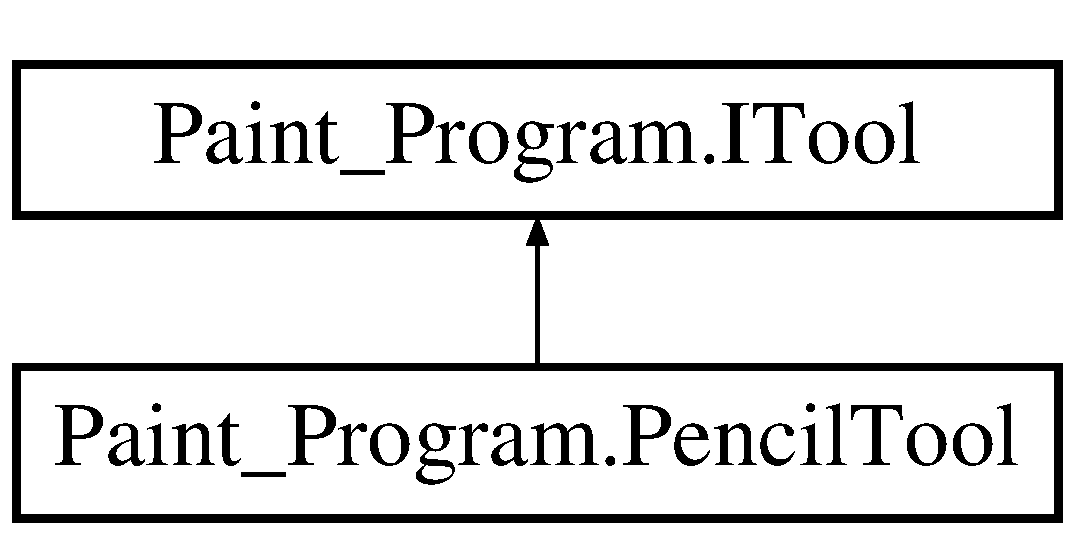
\includegraphics[height=2.000000cm]{class_paint___program_1_1_pencil_tool}
\end{center}
\end{figure}
\subsection*{Public Member Functions}
\begin{DoxyCompactItemize}
\item 
\mbox{\hyperlink{class_paint___program_1_1_pencil_tool_a73363f013795c8814ebf9b297ea9be29}{Pencil\+Tool}} ()
\item 
void \mbox{\hyperlink{class_paint___program_1_1_pencil_tool_ac37cf5b5ccdb57fedfa21326d795cb65}{Init}} ()
\item 
string \mbox{\hyperlink{class_paint___program_1_1_pencil_tool_a91c7f9e9bd173b3f859cbc37f44c4f48}{Get\+Tool\+Icon\+Path}} ()
\item 
void \mbox{\hyperlink{class_paint___program_1_1_pencil_tool_a559e17e6afc05dde7278d4b69b05b12d}{On\+Mouse\+Down}} (object sender, Mouse\+Event\+Args e)
\item 
void \mbox{\hyperlink{class_paint___program_1_1_pencil_tool_a05d86241cc76eaf2abaa94b6ac3f5cfe}{On\+Mouse\+Move}} (object sender, Mouse\+Event\+Args e)
\item 
void \mbox{\hyperlink{class_paint___program_1_1_pencil_tool_ad59c1709d381a33f8363fd15f526eb0e}{On\+Mouse\+Up}} (object sender, Mouse\+Event\+Args e)
\item 
bool \mbox{\hyperlink{class_paint___program_1_1_pencil_tool_abb49751775484b9fcd8ce2e20de98763}{is\+Initalized}} ()
\item 
Bitmap \mbox{\hyperlink{class_paint___program_1_1_pencil_tool_acef50de4028855c4a6be1ff9f63f9b3b}{Get\+Tool\+Layer}} ()
\item 
bool \mbox{\hyperlink{class_paint___program_1_1_pencil_tool_ae41c314454969364d7bdf85e584faf46}{Requires\+Layer\+Data}} ()
\item 
void \mbox{\hyperlink{class_paint___program_1_1_pencil_tool_a4b61261c9e375085bcbac4546a50793e}{Set\+Layer\+Data}} (Bitmap bit)
\item 
string \mbox{\hyperlink{class_paint___program_1_1_pencil_tool_a4805076bc9f2d54b48bb5e76a4e575d9}{Get\+Tool\+Tip}} ()
\item 
void \mbox{\hyperlink{class_paint___program_1_1_pencil_tool_a96ceb2ad71f16fbb361024f58665f6a3}{Update\+Interface\+Layer}} ()
\end{DoxyCompactItemize}
\subsection*{Private Member Functions}
\begin{DoxyCompactItemize}
\item 
void \mbox{\hyperlink{class_paint___program_1_1_pencil_tool_a4666e6bbf0d2716513bf12ae2a5c72f5}{update\+Colors}} ()
\end{DoxyCompactItemize}
\subsection*{Private Attributes}
\begin{DoxyCompactItemize}
\item 
Graphics \mbox{\hyperlink{class_paint___program_1_1_pencil_tool_ab4fb02c2a33bb96d80af3577ca0cfd65}{graphics}}
\item 
int \mbox{\hyperlink{class_paint___program_1_1_pencil_tool_a73493b4b2075f1c675e8eef6e93a39b0}{width}}
\item 
int \mbox{\hyperlink{class_paint___program_1_1_pencil_tool_ae874b99d7cbf60f10803057761873a0e}{height}}
\item 
bool \mbox{\hyperlink{class_paint___program_1_1_pencil_tool_aa4d253416a09bb60caa034b30aa4b178}{b\+Mouse\+Down}}
\item 
bool \mbox{\hyperlink{class_paint___program_1_1_pencil_tool_aa1ceafc9691b146393d86f6f10f4ac50}{b\+Init}}
\item 
Color \mbox{\hyperlink{class_paint___program_1_1_pencil_tool_acd091ded90e4b4e38afe9c730833a021}{c\+Prime}}
\item 
Color \mbox{\hyperlink{class_paint___program_1_1_pencil_tool_a47ee957e8b68e0db3b16acdb7705d185}{c\+Sec}}
\item 
Point \mbox{\hyperlink{class_paint___program_1_1_pencil_tool_ae8087fddbcaec028ff037c4e1d07ece2}{p\+Old}}
\item 
Point \mbox{\hyperlink{class_paint___program_1_1_pencil_tool_a8313fd420ea05ece228551d9d5d15c4d}{p\+New}}
\end{DoxyCompactItemize}


\subsection{Constructor \& Destructor Documentation}
\mbox{\Hypertarget{class_paint___program_1_1_pencil_tool_a73363f013795c8814ebf9b297ea9be29}\label{class_paint___program_1_1_pencil_tool_a73363f013795c8814ebf9b297ea9be29}} 
\index{Paint\+\_\+\+Program\+::\+Pencil\+Tool@{Paint\+\_\+\+Program\+::\+Pencil\+Tool}!Pencil\+Tool@{Pencil\+Tool}}
\index{Pencil\+Tool@{Pencil\+Tool}!Paint\+\_\+\+Program\+::\+Pencil\+Tool@{Paint\+\_\+\+Program\+::\+Pencil\+Tool}}
\subsubsection{\texorpdfstring{Pencil\+Tool()}{PencilTool()}}
{\footnotesize\ttfamily Paint\+\_\+\+Program.\+Pencil\+Tool.\+Pencil\+Tool (\begin{DoxyParamCaption}{ }\end{DoxyParamCaption})\hspace{0.3cm}{\ttfamily [inline]}}



\subsection{Member Function Documentation}
\mbox{\Hypertarget{class_paint___program_1_1_pencil_tool_a91c7f9e9bd173b3f859cbc37f44c4f48}\label{class_paint___program_1_1_pencil_tool_a91c7f9e9bd173b3f859cbc37f44c4f48}} 
\index{Paint\+\_\+\+Program\+::\+Pencil\+Tool@{Paint\+\_\+\+Program\+::\+Pencil\+Tool}!Get\+Tool\+Icon\+Path@{Get\+Tool\+Icon\+Path}}
\index{Get\+Tool\+Icon\+Path@{Get\+Tool\+Icon\+Path}!Paint\+\_\+\+Program\+::\+Pencil\+Tool@{Paint\+\_\+\+Program\+::\+Pencil\+Tool}}
\subsubsection{\texorpdfstring{Get\+Tool\+Icon\+Path()}{GetToolIconPath()}}
{\footnotesize\ttfamily string Paint\+\_\+\+Program.\+Pencil\+Tool.\+Get\+Tool\+Icon\+Path (\begin{DoxyParamCaption}{ }\end{DoxyParamCaption})\hspace{0.3cm}{\ttfamily [inline]}}



Implements \mbox{\hyperlink{interface_paint___program_1_1_i_tool_aa057d2f99c59d7bec0215dcad2da1b72}{Paint\+\_\+\+Program.\+I\+Tool}}.

\mbox{\Hypertarget{class_paint___program_1_1_pencil_tool_acef50de4028855c4a6be1ff9f63f9b3b}\label{class_paint___program_1_1_pencil_tool_acef50de4028855c4a6be1ff9f63f9b3b}} 
\index{Paint\+\_\+\+Program\+::\+Pencil\+Tool@{Paint\+\_\+\+Program\+::\+Pencil\+Tool}!Get\+Tool\+Layer@{Get\+Tool\+Layer}}
\index{Get\+Tool\+Layer@{Get\+Tool\+Layer}!Paint\+\_\+\+Program\+::\+Pencil\+Tool@{Paint\+\_\+\+Program\+::\+Pencil\+Tool}}
\subsubsection{\texorpdfstring{Get\+Tool\+Layer()}{GetToolLayer()}}
{\footnotesize\ttfamily Bitmap Paint\+\_\+\+Program.\+Pencil\+Tool.\+Get\+Tool\+Layer (\begin{DoxyParamCaption}{ }\end{DoxyParamCaption})\hspace{0.3cm}{\ttfamily [inline]}}



Implements \mbox{\hyperlink{interface_paint___program_1_1_i_tool_a9b057905515f42a988c166a6a40318e0}{Paint\+\_\+\+Program.\+I\+Tool}}.

\mbox{\Hypertarget{class_paint___program_1_1_pencil_tool_a4805076bc9f2d54b48bb5e76a4e575d9}\label{class_paint___program_1_1_pencil_tool_a4805076bc9f2d54b48bb5e76a4e575d9}} 
\index{Paint\+\_\+\+Program\+::\+Pencil\+Tool@{Paint\+\_\+\+Program\+::\+Pencil\+Tool}!Get\+Tool\+Tip@{Get\+Tool\+Tip}}
\index{Get\+Tool\+Tip@{Get\+Tool\+Tip}!Paint\+\_\+\+Program\+::\+Pencil\+Tool@{Paint\+\_\+\+Program\+::\+Pencil\+Tool}}
\subsubsection{\texorpdfstring{Get\+Tool\+Tip()}{GetToolTip()}}
{\footnotesize\ttfamily string Paint\+\_\+\+Program.\+Pencil\+Tool.\+Get\+Tool\+Tip (\begin{DoxyParamCaption}{ }\end{DoxyParamCaption})\hspace{0.3cm}{\ttfamily [inline]}}



Implements \mbox{\hyperlink{interface_paint___program_1_1_i_tool_ac11f1591587144b6e74f5767bbf1df56}{Paint\+\_\+\+Program.\+I\+Tool}}.

\mbox{\Hypertarget{class_paint___program_1_1_pencil_tool_ac37cf5b5ccdb57fedfa21326d795cb65}\label{class_paint___program_1_1_pencil_tool_ac37cf5b5ccdb57fedfa21326d795cb65}} 
\index{Paint\+\_\+\+Program\+::\+Pencil\+Tool@{Paint\+\_\+\+Program\+::\+Pencil\+Tool}!Init@{Init}}
\index{Init@{Init}!Paint\+\_\+\+Program\+::\+Pencil\+Tool@{Paint\+\_\+\+Program\+::\+Pencil\+Tool}}
\subsubsection{\texorpdfstring{Init()}{Init()}}
{\footnotesize\ttfamily void Paint\+\_\+\+Program.\+Pencil\+Tool.\+Init (\begin{DoxyParamCaption}{ }\end{DoxyParamCaption})\hspace{0.3cm}{\ttfamily [inline]}}



Implements \mbox{\hyperlink{interface_paint___program_1_1_i_tool_af823123a30fbda34e24e907243241046}{Paint\+\_\+\+Program.\+I\+Tool}}.

\mbox{\Hypertarget{class_paint___program_1_1_pencil_tool_abb49751775484b9fcd8ce2e20de98763}\label{class_paint___program_1_1_pencil_tool_abb49751775484b9fcd8ce2e20de98763}} 
\index{Paint\+\_\+\+Program\+::\+Pencil\+Tool@{Paint\+\_\+\+Program\+::\+Pencil\+Tool}!is\+Initalized@{is\+Initalized}}
\index{is\+Initalized@{is\+Initalized}!Paint\+\_\+\+Program\+::\+Pencil\+Tool@{Paint\+\_\+\+Program\+::\+Pencil\+Tool}}
\subsubsection{\texorpdfstring{is\+Initalized()}{isInitalized()}}
{\footnotesize\ttfamily bool Paint\+\_\+\+Program.\+Pencil\+Tool.\+is\+Initalized (\begin{DoxyParamCaption}{ }\end{DoxyParamCaption})\hspace{0.3cm}{\ttfamily [inline]}}



Implements \mbox{\hyperlink{interface_paint___program_1_1_i_tool_a951b844bcbf47a6c306104fa86be7a5d}{Paint\+\_\+\+Program.\+I\+Tool}}.

\mbox{\Hypertarget{class_paint___program_1_1_pencil_tool_a559e17e6afc05dde7278d4b69b05b12d}\label{class_paint___program_1_1_pencil_tool_a559e17e6afc05dde7278d4b69b05b12d}} 
\index{Paint\+\_\+\+Program\+::\+Pencil\+Tool@{Paint\+\_\+\+Program\+::\+Pencil\+Tool}!On\+Mouse\+Down@{On\+Mouse\+Down}}
\index{On\+Mouse\+Down@{On\+Mouse\+Down}!Paint\+\_\+\+Program\+::\+Pencil\+Tool@{Paint\+\_\+\+Program\+::\+Pencil\+Tool}}
\subsubsection{\texorpdfstring{On\+Mouse\+Down()}{OnMouseDown()}}
{\footnotesize\ttfamily void Paint\+\_\+\+Program.\+Pencil\+Tool.\+On\+Mouse\+Down (\begin{DoxyParamCaption}\item[{object}]{sender,  }\item[{Mouse\+Event\+Args}]{e }\end{DoxyParamCaption})\hspace{0.3cm}{\ttfamily [inline]}}



Implements \mbox{\hyperlink{interface_paint___program_1_1_i_tool_a73d8797f4f2b1e0d8efe8aadcd44e840}{Paint\+\_\+\+Program.\+I\+Tool}}.

\mbox{\Hypertarget{class_paint___program_1_1_pencil_tool_a05d86241cc76eaf2abaa94b6ac3f5cfe}\label{class_paint___program_1_1_pencil_tool_a05d86241cc76eaf2abaa94b6ac3f5cfe}} 
\index{Paint\+\_\+\+Program\+::\+Pencil\+Tool@{Paint\+\_\+\+Program\+::\+Pencil\+Tool}!On\+Mouse\+Move@{On\+Mouse\+Move}}
\index{On\+Mouse\+Move@{On\+Mouse\+Move}!Paint\+\_\+\+Program\+::\+Pencil\+Tool@{Paint\+\_\+\+Program\+::\+Pencil\+Tool}}
\subsubsection{\texorpdfstring{On\+Mouse\+Move()}{OnMouseMove()}}
{\footnotesize\ttfamily void Paint\+\_\+\+Program.\+Pencil\+Tool.\+On\+Mouse\+Move (\begin{DoxyParamCaption}\item[{object}]{sender,  }\item[{Mouse\+Event\+Args}]{e }\end{DoxyParamCaption})\hspace{0.3cm}{\ttfamily [inline]}}



Implements \mbox{\hyperlink{interface_paint___program_1_1_i_tool_a6a1cbe840b5cfc8a9b9463cc21590845}{Paint\+\_\+\+Program.\+I\+Tool}}.

\mbox{\Hypertarget{class_paint___program_1_1_pencil_tool_ad59c1709d381a33f8363fd15f526eb0e}\label{class_paint___program_1_1_pencil_tool_ad59c1709d381a33f8363fd15f526eb0e}} 
\index{Paint\+\_\+\+Program\+::\+Pencil\+Tool@{Paint\+\_\+\+Program\+::\+Pencil\+Tool}!On\+Mouse\+Up@{On\+Mouse\+Up}}
\index{On\+Mouse\+Up@{On\+Mouse\+Up}!Paint\+\_\+\+Program\+::\+Pencil\+Tool@{Paint\+\_\+\+Program\+::\+Pencil\+Tool}}
\subsubsection{\texorpdfstring{On\+Mouse\+Up()}{OnMouseUp()}}
{\footnotesize\ttfamily void Paint\+\_\+\+Program.\+Pencil\+Tool.\+On\+Mouse\+Up (\begin{DoxyParamCaption}\item[{object}]{sender,  }\item[{Mouse\+Event\+Args}]{e }\end{DoxyParamCaption})\hspace{0.3cm}{\ttfamily [inline]}}



Implements \mbox{\hyperlink{interface_paint___program_1_1_i_tool_a47984c2879213022f1684c07f7bba73e}{Paint\+\_\+\+Program.\+I\+Tool}}.

\mbox{\Hypertarget{class_paint___program_1_1_pencil_tool_ae41c314454969364d7bdf85e584faf46}\label{class_paint___program_1_1_pencil_tool_ae41c314454969364d7bdf85e584faf46}} 
\index{Paint\+\_\+\+Program\+::\+Pencil\+Tool@{Paint\+\_\+\+Program\+::\+Pencil\+Tool}!Requires\+Layer\+Data@{Requires\+Layer\+Data}}
\index{Requires\+Layer\+Data@{Requires\+Layer\+Data}!Paint\+\_\+\+Program\+::\+Pencil\+Tool@{Paint\+\_\+\+Program\+::\+Pencil\+Tool}}
\subsubsection{\texorpdfstring{Requires\+Layer\+Data()}{RequiresLayerData()}}
{\footnotesize\ttfamily bool Paint\+\_\+\+Program.\+Pencil\+Tool.\+Requires\+Layer\+Data (\begin{DoxyParamCaption}{ }\end{DoxyParamCaption})\hspace{0.3cm}{\ttfamily [inline]}}



Implements \mbox{\hyperlink{interface_paint___program_1_1_i_tool_a6d45b6c48da8130ae41db3a66cdaef9a}{Paint\+\_\+\+Program.\+I\+Tool}}.

\mbox{\Hypertarget{class_paint___program_1_1_pencil_tool_a4b61261c9e375085bcbac4546a50793e}\label{class_paint___program_1_1_pencil_tool_a4b61261c9e375085bcbac4546a50793e}} 
\index{Paint\+\_\+\+Program\+::\+Pencil\+Tool@{Paint\+\_\+\+Program\+::\+Pencil\+Tool}!Set\+Layer\+Data@{Set\+Layer\+Data}}
\index{Set\+Layer\+Data@{Set\+Layer\+Data}!Paint\+\_\+\+Program\+::\+Pencil\+Tool@{Paint\+\_\+\+Program\+::\+Pencil\+Tool}}
\subsubsection{\texorpdfstring{Set\+Layer\+Data()}{SetLayerData()}}
{\footnotesize\ttfamily void Paint\+\_\+\+Program.\+Pencil\+Tool.\+Set\+Layer\+Data (\begin{DoxyParamCaption}\item[{Bitmap}]{bit }\end{DoxyParamCaption})\hspace{0.3cm}{\ttfamily [inline]}}



Implements \mbox{\hyperlink{interface_paint___program_1_1_i_tool_a2d3e63715dfe04075d27dacf367d1633}{Paint\+\_\+\+Program.\+I\+Tool}}.

\mbox{\Hypertarget{class_paint___program_1_1_pencil_tool_a4666e6bbf0d2716513bf12ae2a5c72f5}\label{class_paint___program_1_1_pencil_tool_a4666e6bbf0d2716513bf12ae2a5c72f5}} 
\index{Paint\+\_\+\+Program\+::\+Pencil\+Tool@{Paint\+\_\+\+Program\+::\+Pencil\+Tool}!update\+Colors@{update\+Colors}}
\index{update\+Colors@{update\+Colors}!Paint\+\_\+\+Program\+::\+Pencil\+Tool@{Paint\+\_\+\+Program\+::\+Pencil\+Tool}}
\subsubsection{\texorpdfstring{update\+Colors()}{updateColors()}}
{\footnotesize\ttfamily void Paint\+\_\+\+Program.\+Pencil\+Tool.\+update\+Colors (\begin{DoxyParamCaption}{ }\end{DoxyParamCaption})\hspace{0.3cm}{\ttfamily [inline]}, {\ttfamily [private]}}

\mbox{\Hypertarget{class_paint___program_1_1_pencil_tool_a96ceb2ad71f16fbb361024f58665f6a3}\label{class_paint___program_1_1_pencil_tool_a96ceb2ad71f16fbb361024f58665f6a3}} 
\index{Paint\+\_\+\+Program\+::\+Pencil\+Tool@{Paint\+\_\+\+Program\+::\+Pencil\+Tool}!Update\+Interface\+Layer@{Update\+Interface\+Layer}}
\index{Update\+Interface\+Layer@{Update\+Interface\+Layer}!Paint\+\_\+\+Program\+::\+Pencil\+Tool@{Paint\+\_\+\+Program\+::\+Pencil\+Tool}}
\subsubsection{\texorpdfstring{Update\+Interface\+Layer()}{UpdateInterfaceLayer()}}
{\footnotesize\ttfamily void Paint\+\_\+\+Program.\+Pencil\+Tool.\+Update\+Interface\+Layer (\begin{DoxyParamCaption}{ }\end{DoxyParamCaption})\hspace{0.3cm}{\ttfamily [inline]}}



Implements \mbox{\hyperlink{interface_paint___program_1_1_i_tool_a36db75d29e88dfd739f658633c40e955}{Paint\+\_\+\+Program.\+I\+Tool}}.



\subsection{Member Data Documentation}
\mbox{\Hypertarget{class_paint___program_1_1_pencil_tool_aa1ceafc9691b146393d86f6f10f4ac50}\label{class_paint___program_1_1_pencil_tool_aa1ceafc9691b146393d86f6f10f4ac50}} 
\index{Paint\+\_\+\+Program\+::\+Pencil\+Tool@{Paint\+\_\+\+Program\+::\+Pencil\+Tool}!b\+Init@{b\+Init}}
\index{b\+Init@{b\+Init}!Paint\+\_\+\+Program\+::\+Pencil\+Tool@{Paint\+\_\+\+Program\+::\+Pencil\+Tool}}
\subsubsection{\texorpdfstring{b\+Init}{bInit}}
{\footnotesize\ttfamily bool Paint\+\_\+\+Program.\+Pencil\+Tool.\+b\+Init\hspace{0.3cm}{\ttfamily [private]}}

\mbox{\Hypertarget{class_paint___program_1_1_pencil_tool_aa4d253416a09bb60caa034b30aa4b178}\label{class_paint___program_1_1_pencil_tool_aa4d253416a09bb60caa034b30aa4b178}} 
\index{Paint\+\_\+\+Program\+::\+Pencil\+Tool@{Paint\+\_\+\+Program\+::\+Pencil\+Tool}!b\+Mouse\+Down@{b\+Mouse\+Down}}
\index{b\+Mouse\+Down@{b\+Mouse\+Down}!Paint\+\_\+\+Program\+::\+Pencil\+Tool@{Paint\+\_\+\+Program\+::\+Pencil\+Tool}}
\subsubsection{\texorpdfstring{b\+Mouse\+Down}{bMouseDown}}
{\footnotesize\ttfamily bool Paint\+\_\+\+Program.\+Pencil\+Tool.\+b\+Mouse\+Down\hspace{0.3cm}{\ttfamily [private]}}

\mbox{\Hypertarget{class_paint___program_1_1_pencil_tool_acd091ded90e4b4e38afe9c730833a021}\label{class_paint___program_1_1_pencil_tool_acd091ded90e4b4e38afe9c730833a021}} 
\index{Paint\+\_\+\+Program\+::\+Pencil\+Tool@{Paint\+\_\+\+Program\+::\+Pencil\+Tool}!c\+Prime@{c\+Prime}}
\index{c\+Prime@{c\+Prime}!Paint\+\_\+\+Program\+::\+Pencil\+Tool@{Paint\+\_\+\+Program\+::\+Pencil\+Tool}}
\subsubsection{\texorpdfstring{c\+Prime}{cPrime}}
{\footnotesize\ttfamily Color Paint\+\_\+\+Program.\+Pencil\+Tool.\+c\+Prime\hspace{0.3cm}{\ttfamily [private]}}

\mbox{\Hypertarget{class_paint___program_1_1_pencil_tool_a47ee957e8b68e0db3b16acdb7705d185}\label{class_paint___program_1_1_pencil_tool_a47ee957e8b68e0db3b16acdb7705d185}} 
\index{Paint\+\_\+\+Program\+::\+Pencil\+Tool@{Paint\+\_\+\+Program\+::\+Pencil\+Tool}!c\+Sec@{c\+Sec}}
\index{c\+Sec@{c\+Sec}!Paint\+\_\+\+Program\+::\+Pencil\+Tool@{Paint\+\_\+\+Program\+::\+Pencil\+Tool}}
\subsubsection{\texorpdfstring{c\+Sec}{cSec}}
{\footnotesize\ttfamily Color Paint\+\_\+\+Program.\+Pencil\+Tool.\+c\+Sec\hspace{0.3cm}{\ttfamily [private]}}

\mbox{\Hypertarget{class_paint___program_1_1_pencil_tool_ab4fb02c2a33bb96d80af3577ca0cfd65}\label{class_paint___program_1_1_pencil_tool_ab4fb02c2a33bb96d80af3577ca0cfd65}} 
\index{Paint\+\_\+\+Program\+::\+Pencil\+Tool@{Paint\+\_\+\+Program\+::\+Pencil\+Tool}!graphics@{graphics}}
\index{graphics@{graphics}!Paint\+\_\+\+Program\+::\+Pencil\+Tool@{Paint\+\_\+\+Program\+::\+Pencil\+Tool}}
\subsubsection{\texorpdfstring{graphics}{graphics}}
{\footnotesize\ttfamily Graphics Paint\+\_\+\+Program.\+Pencil\+Tool.\+graphics\hspace{0.3cm}{\ttfamily [private]}}

\mbox{\Hypertarget{class_paint___program_1_1_pencil_tool_ae874b99d7cbf60f10803057761873a0e}\label{class_paint___program_1_1_pencil_tool_ae874b99d7cbf60f10803057761873a0e}} 
\index{Paint\+\_\+\+Program\+::\+Pencil\+Tool@{Paint\+\_\+\+Program\+::\+Pencil\+Tool}!height@{height}}
\index{height@{height}!Paint\+\_\+\+Program\+::\+Pencil\+Tool@{Paint\+\_\+\+Program\+::\+Pencil\+Tool}}
\subsubsection{\texorpdfstring{height}{height}}
{\footnotesize\ttfamily int Paint\+\_\+\+Program.\+Pencil\+Tool.\+height\hspace{0.3cm}{\ttfamily [private]}}

\mbox{\Hypertarget{class_paint___program_1_1_pencil_tool_a8313fd420ea05ece228551d9d5d15c4d}\label{class_paint___program_1_1_pencil_tool_a8313fd420ea05ece228551d9d5d15c4d}} 
\index{Paint\+\_\+\+Program\+::\+Pencil\+Tool@{Paint\+\_\+\+Program\+::\+Pencil\+Tool}!p\+New@{p\+New}}
\index{p\+New@{p\+New}!Paint\+\_\+\+Program\+::\+Pencil\+Tool@{Paint\+\_\+\+Program\+::\+Pencil\+Tool}}
\subsubsection{\texorpdfstring{p\+New}{pNew}}
{\footnotesize\ttfamily Point Paint\+\_\+\+Program.\+Pencil\+Tool.\+p\+New\hspace{0.3cm}{\ttfamily [private]}}

\mbox{\Hypertarget{class_paint___program_1_1_pencil_tool_ae8087fddbcaec028ff037c4e1d07ece2}\label{class_paint___program_1_1_pencil_tool_ae8087fddbcaec028ff037c4e1d07ece2}} 
\index{Paint\+\_\+\+Program\+::\+Pencil\+Tool@{Paint\+\_\+\+Program\+::\+Pencil\+Tool}!p\+Old@{p\+Old}}
\index{p\+Old@{p\+Old}!Paint\+\_\+\+Program\+::\+Pencil\+Tool@{Paint\+\_\+\+Program\+::\+Pencil\+Tool}}
\subsubsection{\texorpdfstring{p\+Old}{pOld}}
{\footnotesize\ttfamily Point Paint\+\_\+\+Program.\+Pencil\+Tool.\+p\+Old\hspace{0.3cm}{\ttfamily [private]}}

\mbox{\Hypertarget{class_paint___program_1_1_pencil_tool_a73493b4b2075f1c675e8eef6e93a39b0}\label{class_paint___program_1_1_pencil_tool_a73493b4b2075f1c675e8eef6e93a39b0}} 
\index{Paint\+\_\+\+Program\+::\+Pencil\+Tool@{Paint\+\_\+\+Program\+::\+Pencil\+Tool}!width@{width}}
\index{width@{width}!Paint\+\_\+\+Program\+::\+Pencil\+Tool@{Paint\+\_\+\+Program\+::\+Pencil\+Tool}}
\subsubsection{\texorpdfstring{width}{width}}
{\footnotesize\ttfamily int Paint\+\_\+\+Program.\+Pencil\+Tool.\+width\hspace{0.3cm}{\ttfamily [private]}}



The documentation for this class was generated from the following file\+:\begin{DoxyCompactItemize}
\item 
Paint Program/\mbox{\hyperlink{_pencil_tool_8cs}{Pencil\+Tool.\+cs}}\end{DoxyCompactItemize}

\hypertarget{class_paint___program_1_1_program}{}\section{Paint\+\_\+\+Program.\+Program Class Reference}
\label{class_paint___program_1_1_program}\index{Paint\+\_\+\+Program.\+Program@{Paint\+\_\+\+Program.\+Program}}
\subsection*{Static Private Member Functions}
\begin{DoxyCompactItemize}
\item 
static void \mbox{\hyperlink{class_paint___program_1_1_program_a0586d6d89a54c2fecfbb3fd893329c1f}{Main}} ()
\begin{DoxyCompactList}\small\item\em The main entry point for the application. \end{DoxyCompactList}\end{DoxyCompactItemize}


\subsection{Member Function Documentation}
\mbox{\Hypertarget{class_paint___program_1_1_program_a0586d6d89a54c2fecfbb3fd893329c1f}\label{class_paint___program_1_1_program_a0586d6d89a54c2fecfbb3fd893329c1f}} 
\index{Paint\+\_\+\+Program\+::\+Program@{Paint\+\_\+\+Program\+::\+Program}!Main@{Main}}
\index{Main@{Main}!Paint\+\_\+\+Program\+::\+Program@{Paint\+\_\+\+Program\+::\+Program}}
\subsubsection{\texorpdfstring{Main()}{Main()}}
{\footnotesize\ttfamily static void Paint\+\_\+\+Program.\+Program.\+Main (\begin{DoxyParamCaption}{ }\end{DoxyParamCaption})\hspace{0.3cm}{\ttfamily [inline]}, {\ttfamily [static]}, {\ttfamily [private]}}



The main entry point for the application. 



The documentation for this class was generated from the following file\+:\begin{DoxyCompactItemize}
\item 
Paint Program/\mbox{\hyperlink{_program_8cs}{Program.\+cs}}\end{DoxyCompactItemize}

\hypertarget{class_paint___program_1_1_project_load}{}\section{Paint\+\_\+\+Program.\+Project\+Load Class Reference}
\label{class_paint___program_1_1_project_load}\index{Paint\+\_\+\+Program.\+Project\+Load@{Paint\+\_\+\+Program.\+Project\+Load}}
\subsection*{Public Member Functions}
\begin{DoxyCompactItemize}
\item 
\mbox{\hyperlink{class_paint___program_1_1_project_load_ac157ba176be963e2fde2f6971463c1de}{Project\+Load}} ()
\item 
string \mbox{\hyperlink{class_paint___program_1_1_project_load_ab585a79ec6685412d6c0cf3823a44182}{get\+Result\+Message}} ()
\item 
Bitmap \mbox{\hyperlink{class_paint___program_1_1_project_load_acf6d9bc4b31f71674344fd5436a907b1}{Bitmap\+From\+Source}} (Bitmap\+Source bitmapsource)
\end{DoxyCompactItemize}
\subsection*{Static Public Member Functions}
\begin{DoxyCompactItemize}
\item 
static void \mbox{\hyperlink{class_paint___program_1_1_project_load_a1ee7e642eae28f2bfe36ef04198e467c}{Delete\+Directory}} (string target\+\_\+dir)
\end{DoxyCompactItemize}
\subsection*{Private Member Functions}
\begin{DoxyCompactItemize}
\item 
void \mbox{\hyperlink{class_paint___program_1_1_project_load_aaafd3511899db9404705b14a9e471704}{do\+Open}} (Open\+File\+Dialog ofd)
\end{DoxyCompactItemize}
\subsection*{Private Attributes}
\begin{DoxyCompactItemize}
\item 
string \mbox{\hyperlink{class_paint___program_1_1_project_load_a9db3022290634d4c0c7fad302d03eaba}{Result}}
\end{DoxyCompactItemize}


\subsection{Constructor \& Destructor Documentation}
\mbox{\Hypertarget{class_paint___program_1_1_project_load_ac157ba176be963e2fde2f6971463c1de}\label{class_paint___program_1_1_project_load_ac157ba176be963e2fde2f6971463c1de}} 
\index{Paint\+\_\+\+Program\+::\+Project\+Load@{Paint\+\_\+\+Program\+::\+Project\+Load}!Project\+Load@{Project\+Load}}
\index{Project\+Load@{Project\+Load}!Paint\+\_\+\+Program\+::\+Project\+Load@{Paint\+\_\+\+Program\+::\+Project\+Load}}
\subsubsection{\texorpdfstring{Project\+Load()}{ProjectLoad()}}
{\footnotesize\ttfamily Paint\+\_\+\+Program.\+Project\+Load.\+Project\+Load (\begin{DoxyParamCaption}{ }\end{DoxyParamCaption})\hspace{0.3cm}{\ttfamily [inline]}}



\subsection{Member Function Documentation}
\mbox{\Hypertarget{class_paint___program_1_1_project_load_acf6d9bc4b31f71674344fd5436a907b1}\label{class_paint___program_1_1_project_load_acf6d9bc4b31f71674344fd5436a907b1}} 
\index{Paint\+\_\+\+Program\+::\+Project\+Load@{Paint\+\_\+\+Program\+::\+Project\+Load}!Bitmap\+From\+Source@{Bitmap\+From\+Source}}
\index{Bitmap\+From\+Source@{Bitmap\+From\+Source}!Paint\+\_\+\+Program\+::\+Project\+Load@{Paint\+\_\+\+Program\+::\+Project\+Load}}
\subsubsection{\texorpdfstring{Bitmap\+From\+Source()}{BitmapFromSource()}}
{\footnotesize\ttfamily Bitmap Paint\+\_\+\+Program.\+Project\+Load.\+Bitmap\+From\+Source (\begin{DoxyParamCaption}\item[{Bitmap\+Source}]{bitmapsource }\end{DoxyParamCaption})\hspace{0.3cm}{\ttfamily [inline]}}

\mbox{\Hypertarget{class_paint___program_1_1_project_load_a1ee7e642eae28f2bfe36ef04198e467c}\label{class_paint___program_1_1_project_load_a1ee7e642eae28f2bfe36ef04198e467c}} 
\index{Paint\+\_\+\+Program\+::\+Project\+Load@{Paint\+\_\+\+Program\+::\+Project\+Load}!Delete\+Directory@{Delete\+Directory}}
\index{Delete\+Directory@{Delete\+Directory}!Paint\+\_\+\+Program\+::\+Project\+Load@{Paint\+\_\+\+Program\+::\+Project\+Load}}
\subsubsection{\texorpdfstring{Delete\+Directory()}{DeleteDirectory()}}
{\footnotesize\ttfamily static void Paint\+\_\+\+Program.\+Project\+Load.\+Delete\+Directory (\begin{DoxyParamCaption}\item[{string}]{target\+\_\+dir }\end{DoxyParamCaption})\hspace{0.3cm}{\ttfamily [inline]}, {\ttfamily [static]}}

\mbox{\Hypertarget{class_paint___program_1_1_project_load_aaafd3511899db9404705b14a9e471704}\label{class_paint___program_1_1_project_load_aaafd3511899db9404705b14a9e471704}} 
\index{Paint\+\_\+\+Program\+::\+Project\+Load@{Paint\+\_\+\+Program\+::\+Project\+Load}!do\+Open@{do\+Open}}
\index{do\+Open@{do\+Open}!Paint\+\_\+\+Program\+::\+Project\+Load@{Paint\+\_\+\+Program\+::\+Project\+Load}}
\subsubsection{\texorpdfstring{do\+Open()}{doOpen()}}
{\footnotesize\ttfamily void Paint\+\_\+\+Program.\+Project\+Load.\+do\+Open (\begin{DoxyParamCaption}\item[{Open\+File\+Dialog}]{ofd }\end{DoxyParamCaption})\hspace{0.3cm}{\ttfamily [inline]}, {\ttfamily [private]}}

\mbox{\Hypertarget{class_paint___program_1_1_project_load_ab585a79ec6685412d6c0cf3823a44182}\label{class_paint___program_1_1_project_load_ab585a79ec6685412d6c0cf3823a44182}} 
\index{Paint\+\_\+\+Program\+::\+Project\+Load@{Paint\+\_\+\+Program\+::\+Project\+Load}!get\+Result\+Message@{get\+Result\+Message}}
\index{get\+Result\+Message@{get\+Result\+Message}!Paint\+\_\+\+Program\+::\+Project\+Load@{Paint\+\_\+\+Program\+::\+Project\+Load}}
\subsubsection{\texorpdfstring{get\+Result\+Message()}{getResultMessage()}}
{\footnotesize\ttfamily string Paint\+\_\+\+Program.\+Project\+Load.\+get\+Result\+Message (\begin{DoxyParamCaption}{ }\end{DoxyParamCaption})\hspace{0.3cm}{\ttfamily [inline]}}



\subsection{Member Data Documentation}
\mbox{\Hypertarget{class_paint___program_1_1_project_load_a9db3022290634d4c0c7fad302d03eaba}\label{class_paint___program_1_1_project_load_a9db3022290634d4c0c7fad302d03eaba}} 
\index{Paint\+\_\+\+Program\+::\+Project\+Load@{Paint\+\_\+\+Program\+::\+Project\+Load}!Result@{Result}}
\index{Result@{Result}!Paint\+\_\+\+Program\+::\+Project\+Load@{Paint\+\_\+\+Program\+::\+Project\+Load}}
\subsubsection{\texorpdfstring{Result}{Result}}
{\footnotesize\ttfamily string Paint\+\_\+\+Program.\+Project\+Load.\+Result\hspace{0.3cm}{\ttfamily [private]}}



The documentation for this class was generated from the following file\+:\begin{DoxyCompactItemize}
\item 
Paint Program/\mbox{\hyperlink{_project_load_8cs}{Project\+Load.\+cs}}\end{DoxyCompactItemize}

\hypertarget{class_paint___program_1_1_project_save}{}\section{Paint\+\_\+\+Program.\+Project\+Save Class Reference}
\label{class_paint___program_1_1_project_save}\index{Paint\+\_\+\+Program.\+Project\+Save@{Paint\+\_\+\+Program.\+Project\+Save}}
\subsection*{Public Member Functions}
\begin{DoxyCompactItemize}
\item 
\mbox{\hyperlink{class_paint___program_1_1_project_save_aa96a77459d2ebc0f5b7ae6b5eb21bbe5}{Project\+Save}} ()
\end{DoxyCompactItemize}
\subsection*{Private Member Functions}
\begin{DoxyCompactItemize}
\item 
void \mbox{\hyperlink{class_paint___program_1_1_project_save_aa28784aaca38fc6348c62daf33b31898}{do\+Save}} (Save\+File\+Dialog sfd)
\end{DoxyCompactItemize}


\subsection{Constructor \& Destructor Documentation}
\mbox{\Hypertarget{class_paint___program_1_1_project_save_aa96a77459d2ebc0f5b7ae6b5eb21bbe5}\label{class_paint___program_1_1_project_save_aa96a77459d2ebc0f5b7ae6b5eb21bbe5}} 
\index{Paint\+\_\+\+Program\+::\+Project\+Save@{Paint\+\_\+\+Program\+::\+Project\+Save}!Project\+Save@{Project\+Save}}
\index{Project\+Save@{Project\+Save}!Paint\+\_\+\+Program\+::\+Project\+Save@{Paint\+\_\+\+Program\+::\+Project\+Save}}
\subsubsection{\texorpdfstring{Project\+Save()}{ProjectSave()}}
{\footnotesize\ttfamily Paint\+\_\+\+Program.\+Project\+Save.\+Project\+Save (\begin{DoxyParamCaption}{ }\end{DoxyParamCaption})\hspace{0.3cm}{\ttfamily [inline]}}



\subsection{Member Function Documentation}
\mbox{\Hypertarget{class_paint___program_1_1_project_save_aa28784aaca38fc6348c62daf33b31898}\label{class_paint___program_1_1_project_save_aa28784aaca38fc6348c62daf33b31898}} 
\index{Paint\+\_\+\+Program\+::\+Project\+Save@{Paint\+\_\+\+Program\+::\+Project\+Save}!do\+Save@{do\+Save}}
\index{do\+Save@{do\+Save}!Paint\+\_\+\+Program\+::\+Project\+Save@{Paint\+\_\+\+Program\+::\+Project\+Save}}
\subsubsection{\texorpdfstring{do\+Save()}{doSave()}}
{\footnotesize\ttfamily void Paint\+\_\+\+Program.\+Project\+Save.\+do\+Save (\begin{DoxyParamCaption}\item[{Save\+File\+Dialog}]{sfd }\end{DoxyParamCaption})\hspace{0.3cm}{\ttfamily [inline]}, {\ttfamily [private]}}



The documentation for this class was generated from the following file\+:\begin{DoxyCompactItemize}
\item 
Paint Program/\mbox{\hyperlink{_project_save_8cs}{Project\+Save.\+cs}}\end{DoxyCompactItemize}

\hypertarget{class_paint___program_1_1_save_to_drive}{}\section{Paint\+\_\+\+Program.\+Save\+To\+Drive Class Reference}
\label{class_paint___program_1_1_save_to_drive}\index{Paint\+\_\+\+Program.\+Save\+To\+Drive@{Paint\+\_\+\+Program.\+Save\+To\+Drive}}
\subsection*{Public Member Functions}
\begin{DoxyCompactItemize}
\item 
\mbox{\hyperlink{class_paint___program_1_1_save_to_drive_aa5f7d65ca88d6e2dcb07a59dbd118fce}{Save\+To\+Drive}} (string file\+Name, string file\+Type)
\item 
void \mbox{\hyperlink{class_paint___program_1_1_save_to_drive_a57ff1c0b94b46731df43a04f2eb28f07}{do\+Save}} (Bitmap bm, string filename, string filetype, object sender, Do\+Work\+Event\+Args args)
\item 
void \mbox{\hyperlink{class_paint___program_1_1_save_to_drive_a10a9b341d476f9f773e72c0551545aff}{do\+Save\+Anim\+Gif}} (string filename, object sender, Do\+Work\+Event\+Args args)
\item 
void \mbox{\hyperlink{class_paint___program_1_1_save_to_drive_a76739416bfdb48941e22807b8ae03dea}{do\+Save\+Project}} (string filename, object sender, Do\+Work\+Event\+Args args)
\end{DoxyCompactItemize}


\subsection{Constructor \& Destructor Documentation}
\mbox{\Hypertarget{class_paint___program_1_1_save_to_drive_aa5f7d65ca88d6e2dcb07a59dbd118fce}\label{class_paint___program_1_1_save_to_drive_aa5f7d65ca88d6e2dcb07a59dbd118fce}} 
\index{Paint\+\_\+\+Program\+::\+Save\+To\+Drive@{Paint\+\_\+\+Program\+::\+Save\+To\+Drive}!Save\+To\+Drive@{Save\+To\+Drive}}
\index{Save\+To\+Drive@{Save\+To\+Drive}!Paint\+\_\+\+Program\+::\+Save\+To\+Drive@{Paint\+\_\+\+Program\+::\+Save\+To\+Drive}}
\subsubsection{\texorpdfstring{Save\+To\+Drive()}{SaveToDrive()}}
{\footnotesize\ttfamily Paint\+\_\+\+Program.\+Save\+To\+Drive.\+Save\+To\+Drive (\begin{DoxyParamCaption}\item[{string}]{file\+Name,  }\item[{string}]{file\+Type }\end{DoxyParamCaption})\hspace{0.3cm}{\ttfamily [inline]}}



\subsection{Member Function Documentation}
\mbox{\Hypertarget{class_paint___program_1_1_save_to_drive_a57ff1c0b94b46731df43a04f2eb28f07}\label{class_paint___program_1_1_save_to_drive_a57ff1c0b94b46731df43a04f2eb28f07}} 
\index{Paint\+\_\+\+Program\+::\+Save\+To\+Drive@{Paint\+\_\+\+Program\+::\+Save\+To\+Drive}!do\+Save@{do\+Save}}
\index{do\+Save@{do\+Save}!Paint\+\_\+\+Program\+::\+Save\+To\+Drive@{Paint\+\_\+\+Program\+::\+Save\+To\+Drive}}
\subsubsection{\texorpdfstring{do\+Save()}{doSave()}}
{\footnotesize\ttfamily void Paint\+\_\+\+Program.\+Save\+To\+Drive.\+do\+Save (\begin{DoxyParamCaption}\item[{Bitmap}]{bm,  }\item[{string}]{filename,  }\item[{string}]{filetype,  }\item[{object}]{sender,  }\item[{Do\+Work\+Event\+Args}]{args }\end{DoxyParamCaption})\hspace{0.3cm}{\ttfamily [inline]}}

\mbox{\Hypertarget{class_paint___program_1_1_save_to_drive_a10a9b341d476f9f773e72c0551545aff}\label{class_paint___program_1_1_save_to_drive_a10a9b341d476f9f773e72c0551545aff}} 
\index{Paint\+\_\+\+Program\+::\+Save\+To\+Drive@{Paint\+\_\+\+Program\+::\+Save\+To\+Drive}!do\+Save\+Anim\+Gif@{do\+Save\+Anim\+Gif}}
\index{do\+Save\+Anim\+Gif@{do\+Save\+Anim\+Gif}!Paint\+\_\+\+Program\+::\+Save\+To\+Drive@{Paint\+\_\+\+Program\+::\+Save\+To\+Drive}}
\subsubsection{\texorpdfstring{do\+Save\+Anim\+Gif()}{doSaveAnimGif()}}
{\footnotesize\ttfamily void Paint\+\_\+\+Program.\+Save\+To\+Drive.\+do\+Save\+Anim\+Gif (\begin{DoxyParamCaption}\item[{string}]{filename,  }\item[{object}]{sender,  }\item[{Do\+Work\+Event\+Args}]{args }\end{DoxyParamCaption})\hspace{0.3cm}{\ttfamily [inline]}}

\mbox{\Hypertarget{class_paint___program_1_1_save_to_drive_a76739416bfdb48941e22807b8ae03dea}\label{class_paint___program_1_1_save_to_drive_a76739416bfdb48941e22807b8ae03dea}} 
\index{Paint\+\_\+\+Program\+::\+Save\+To\+Drive@{Paint\+\_\+\+Program\+::\+Save\+To\+Drive}!do\+Save\+Project@{do\+Save\+Project}}
\index{do\+Save\+Project@{do\+Save\+Project}!Paint\+\_\+\+Program\+::\+Save\+To\+Drive@{Paint\+\_\+\+Program\+::\+Save\+To\+Drive}}
\subsubsection{\texorpdfstring{do\+Save\+Project()}{doSaveProject()}}
{\footnotesize\ttfamily void Paint\+\_\+\+Program.\+Save\+To\+Drive.\+do\+Save\+Project (\begin{DoxyParamCaption}\item[{string}]{filename,  }\item[{object}]{sender,  }\item[{Do\+Work\+Event\+Args}]{args }\end{DoxyParamCaption})\hspace{0.3cm}{\ttfamily [inline]}}



The documentation for this class was generated from the following file\+:\begin{DoxyCompactItemize}
\item 
Paint Program/\mbox{\hyperlink{_save_to_drive_8cs}{Save\+To\+Drive.\+cs}}\end{DoxyCompactItemize}

\hypertarget{class_paint___program_1_1_selection_tool}{}\section{Paint\+\_\+\+Program.\+Selection\+Tool Class Reference}
\label{class_paint___program_1_1_selection_tool}\index{Paint\+\_\+\+Program.\+Selection\+Tool@{Paint\+\_\+\+Program.\+Selection\+Tool}}
Inheritance diagram for Paint\+\_\+\+Program.\+Selection\+Tool\+:\begin{figure}[H]
\begin{center}
\leavevmode
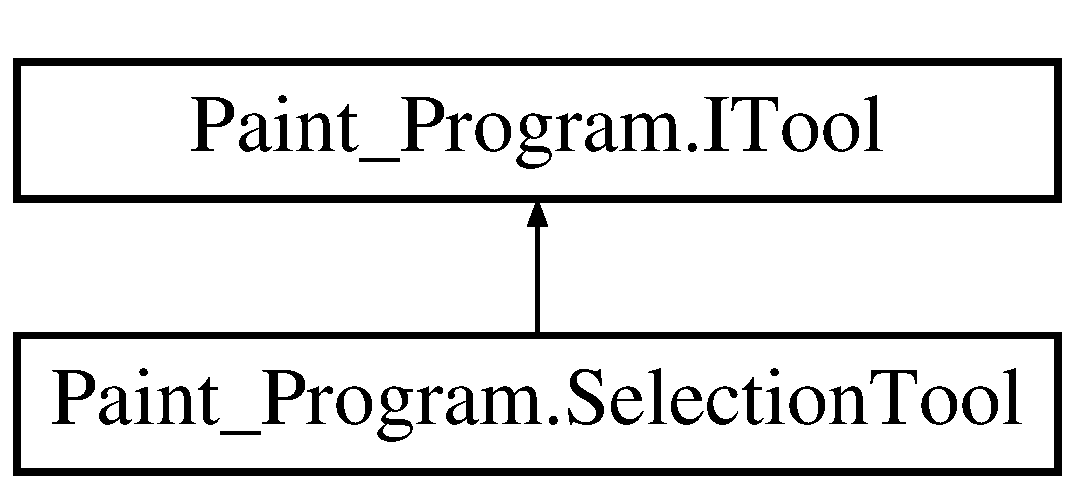
\includegraphics[height=2.000000cm]{class_paint___program_1_1_selection_tool}
\end{center}
\end{figure}
\subsection*{Public Member Functions}
\begin{DoxyCompactItemize}
\item 
void \mbox{\hyperlink{class_paint___program_1_1_selection_tool_afadcc35f14a6e833a09c225a4efc1ed7}{Init}} ()
\item 
string \mbox{\hyperlink{class_paint___program_1_1_selection_tool_ac93f281cfcc677551b140c350661d9df}{Get\+Tool\+Icon\+Path}} ()
\item 
Bitmap \mbox{\hyperlink{class_paint___program_1_1_selection_tool_ad8d0b5e9cf0486f7e3815db1536de03d}{Get\+Tool\+Layer}} ()
\item 
bool \mbox{\hyperlink{class_paint___program_1_1_selection_tool_a04d5a1f8ed1eb4fb786a09cf122b0200}{is\+Initalized}} ()
\item 
void \mbox{\hyperlink{class_paint___program_1_1_selection_tool_a1134ee98cfa46d98871716ede5f08d1f}{On\+Mouse\+Down}} (object sender, Mouse\+Event\+Args e)
\item 
void \mbox{\hyperlink{class_paint___program_1_1_selection_tool_adec8eaad22f0c7ac1a744247c87e16bc}{On\+Mouse\+Move}} (object sender, Mouse\+Event\+Args e)
\item 
void \mbox{\hyperlink{class_paint___program_1_1_selection_tool_aa271d61b0d9c182e9bba5fab0b2893eb}{On\+Mouse\+Up}} (object sender, Mouse\+Event\+Args e)
\item 
bool \mbox{\hyperlink{class_paint___program_1_1_selection_tool_a3e97ebc6bc62f194b42e2acdd24a498f}{Requires\+Layer\+Data}} ()
\item 
void \mbox{\hyperlink{class_paint___program_1_1_selection_tool_a3975a7e8ef98db8f1edaa5fd586fa486}{Set\+Layer\+Data}} (Bitmap bit)
\item 
string \mbox{\hyperlink{class_paint___program_1_1_selection_tool_a27eaa7276db68cea198c96a30b3dba9e}{Get\+Tool\+Tip}} ()
\item 
void \mbox{\hyperlink{class_paint___program_1_1_selection_tool_ac8b5875e3a8a10cac0c4e37f286c0e2e}{Clean}} ()
\item 
void \mbox{\hyperlink{class_paint___program_1_1_selection_tool_ad541275f644867e4fb0d95db8a723b14}{Update\+Interface\+Layer}} ()
\end{DoxyCompactItemize}
\subsection*{Private Attributes}
\begin{DoxyCompactItemize}
\item 
bool \mbox{\hyperlink{class_paint___program_1_1_selection_tool_a11340d6e8c518de6c2e2727bdb9b8479}{is\+Init}} = false
\item 
Point \mbox{\hyperlink{class_paint___program_1_1_selection_tool_aa222db7e2507d4a78432ee18f21c2bec}{p1}}
\item 
Point \mbox{\hyperlink{class_paint___program_1_1_selection_tool_adc89856894483623d0735ffc031fe883}{p2}}
\item 
Point \mbox{\hyperlink{class_paint___program_1_1_selection_tool_ad9d0cc8becec7128bf025fb17d957a90}{p\+Old}}
\item 
Point \mbox{\hyperlink{class_paint___program_1_1_selection_tool_a90bc3a955ec60db4d812d20c54cd42ce}{p\+New}}
\item 
Bitmap \mbox{\hyperlink{class_paint___program_1_1_selection_tool_a90ad41bebfb20e575899626d62c88b1a}{b\+Edit}}
\end{DoxyCompactItemize}


\subsection{Member Function Documentation}
\mbox{\Hypertarget{class_paint___program_1_1_selection_tool_ac8b5875e3a8a10cac0c4e37f286c0e2e}\label{class_paint___program_1_1_selection_tool_ac8b5875e3a8a10cac0c4e37f286c0e2e}} 
\index{Paint\+\_\+\+Program\+::\+Selection\+Tool@{Paint\+\_\+\+Program\+::\+Selection\+Tool}!Clean@{Clean}}
\index{Clean@{Clean}!Paint\+\_\+\+Program\+::\+Selection\+Tool@{Paint\+\_\+\+Program\+::\+Selection\+Tool}}
\subsubsection{\texorpdfstring{Clean()}{Clean()}}
{\footnotesize\ttfamily void Paint\+\_\+\+Program.\+Selection\+Tool.\+Clean (\begin{DoxyParamCaption}{ }\end{DoxyParamCaption})\hspace{0.3cm}{\ttfamily [inline]}}

\mbox{\Hypertarget{class_paint___program_1_1_selection_tool_ac93f281cfcc677551b140c350661d9df}\label{class_paint___program_1_1_selection_tool_ac93f281cfcc677551b140c350661d9df}} 
\index{Paint\+\_\+\+Program\+::\+Selection\+Tool@{Paint\+\_\+\+Program\+::\+Selection\+Tool}!Get\+Tool\+Icon\+Path@{Get\+Tool\+Icon\+Path}}
\index{Get\+Tool\+Icon\+Path@{Get\+Tool\+Icon\+Path}!Paint\+\_\+\+Program\+::\+Selection\+Tool@{Paint\+\_\+\+Program\+::\+Selection\+Tool}}
\subsubsection{\texorpdfstring{Get\+Tool\+Icon\+Path()}{GetToolIconPath()}}
{\footnotesize\ttfamily string Paint\+\_\+\+Program.\+Selection\+Tool.\+Get\+Tool\+Icon\+Path (\begin{DoxyParamCaption}{ }\end{DoxyParamCaption})\hspace{0.3cm}{\ttfamily [inline]}}



Implements \mbox{\hyperlink{interface_paint___program_1_1_i_tool_aa057d2f99c59d7bec0215dcad2da1b72}{Paint\+\_\+\+Program.\+I\+Tool}}.

\mbox{\Hypertarget{class_paint___program_1_1_selection_tool_ad8d0b5e9cf0486f7e3815db1536de03d}\label{class_paint___program_1_1_selection_tool_ad8d0b5e9cf0486f7e3815db1536de03d}} 
\index{Paint\+\_\+\+Program\+::\+Selection\+Tool@{Paint\+\_\+\+Program\+::\+Selection\+Tool}!Get\+Tool\+Layer@{Get\+Tool\+Layer}}
\index{Get\+Tool\+Layer@{Get\+Tool\+Layer}!Paint\+\_\+\+Program\+::\+Selection\+Tool@{Paint\+\_\+\+Program\+::\+Selection\+Tool}}
\subsubsection{\texorpdfstring{Get\+Tool\+Layer()}{GetToolLayer()}}
{\footnotesize\ttfamily Bitmap Paint\+\_\+\+Program.\+Selection\+Tool.\+Get\+Tool\+Layer (\begin{DoxyParamCaption}{ }\end{DoxyParamCaption})\hspace{0.3cm}{\ttfamily [inline]}}



Implements \mbox{\hyperlink{interface_paint___program_1_1_i_tool_a9b057905515f42a988c166a6a40318e0}{Paint\+\_\+\+Program.\+I\+Tool}}.

\mbox{\Hypertarget{class_paint___program_1_1_selection_tool_a27eaa7276db68cea198c96a30b3dba9e}\label{class_paint___program_1_1_selection_tool_a27eaa7276db68cea198c96a30b3dba9e}} 
\index{Paint\+\_\+\+Program\+::\+Selection\+Tool@{Paint\+\_\+\+Program\+::\+Selection\+Tool}!Get\+Tool\+Tip@{Get\+Tool\+Tip}}
\index{Get\+Tool\+Tip@{Get\+Tool\+Tip}!Paint\+\_\+\+Program\+::\+Selection\+Tool@{Paint\+\_\+\+Program\+::\+Selection\+Tool}}
\subsubsection{\texorpdfstring{Get\+Tool\+Tip()}{GetToolTip()}}
{\footnotesize\ttfamily string Paint\+\_\+\+Program.\+Selection\+Tool.\+Get\+Tool\+Tip (\begin{DoxyParamCaption}{ }\end{DoxyParamCaption})\hspace{0.3cm}{\ttfamily [inline]}}



Implements \mbox{\hyperlink{interface_paint___program_1_1_i_tool_ac11f1591587144b6e74f5767bbf1df56}{Paint\+\_\+\+Program.\+I\+Tool}}.

\mbox{\Hypertarget{class_paint___program_1_1_selection_tool_afadcc35f14a6e833a09c225a4efc1ed7}\label{class_paint___program_1_1_selection_tool_afadcc35f14a6e833a09c225a4efc1ed7}} 
\index{Paint\+\_\+\+Program\+::\+Selection\+Tool@{Paint\+\_\+\+Program\+::\+Selection\+Tool}!Init@{Init}}
\index{Init@{Init}!Paint\+\_\+\+Program\+::\+Selection\+Tool@{Paint\+\_\+\+Program\+::\+Selection\+Tool}}
\subsubsection{\texorpdfstring{Init()}{Init()}}
{\footnotesize\ttfamily void Paint\+\_\+\+Program.\+Selection\+Tool.\+Init (\begin{DoxyParamCaption}{ }\end{DoxyParamCaption})\hspace{0.3cm}{\ttfamily [inline]}}



Implements \mbox{\hyperlink{interface_paint___program_1_1_i_tool_af823123a30fbda34e24e907243241046}{Paint\+\_\+\+Program.\+I\+Tool}}.

\mbox{\Hypertarget{class_paint___program_1_1_selection_tool_a04d5a1f8ed1eb4fb786a09cf122b0200}\label{class_paint___program_1_1_selection_tool_a04d5a1f8ed1eb4fb786a09cf122b0200}} 
\index{Paint\+\_\+\+Program\+::\+Selection\+Tool@{Paint\+\_\+\+Program\+::\+Selection\+Tool}!is\+Initalized@{is\+Initalized}}
\index{is\+Initalized@{is\+Initalized}!Paint\+\_\+\+Program\+::\+Selection\+Tool@{Paint\+\_\+\+Program\+::\+Selection\+Tool}}
\subsubsection{\texorpdfstring{is\+Initalized()}{isInitalized()}}
{\footnotesize\ttfamily bool Paint\+\_\+\+Program.\+Selection\+Tool.\+is\+Initalized (\begin{DoxyParamCaption}{ }\end{DoxyParamCaption})\hspace{0.3cm}{\ttfamily [inline]}}



Implements \mbox{\hyperlink{interface_paint___program_1_1_i_tool_a951b844bcbf47a6c306104fa86be7a5d}{Paint\+\_\+\+Program.\+I\+Tool}}.

\mbox{\Hypertarget{class_paint___program_1_1_selection_tool_a1134ee98cfa46d98871716ede5f08d1f}\label{class_paint___program_1_1_selection_tool_a1134ee98cfa46d98871716ede5f08d1f}} 
\index{Paint\+\_\+\+Program\+::\+Selection\+Tool@{Paint\+\_\+\+Program\+::\+Selection\+Tool}!On\+Mouse\+Down@{On\+Mouse\+Down}}
\index{On\+Mouse\+Down@{On\+Mouse\+Down}!Paint\+\_\+\+Program\+::\+Selection\+Tool@{Paint\+\_\+\+Program\+::\+Selection\+Tool}}
\subsubsection{\texorpdfstring{On\+Mouse\+Down()}{OnMouseDown()}}
{\footnotesize\ttfamily void Paint\+\_\+\+Program.\+Selection\+Tool.\+On\+Mouse\+Down (\begin{DoxyParamCaption}\item[{object}]{sender,  }\item[{Mouse\+Event\+Args}]{e }\end{DoxyParamCaption})\hspace{0.3cm}{\ttfamily [inline]}}



Implements \mbox{\hyperlink{interface_paint___program_1_1_i_tool_a73d8797f4f2b1e0d8efe8aadcd44e840}{Paint\+\_\+\+Program.\+I\+Tool}}.

\mbox{\Hypertarget{class_paint___program_1_1_selection_tool_adec8eaad22f0c7ac1a744247c87e16bc}\label{class_paint___program_1_1_selection_tool_adec8eaad22f0c7ac1a744247c87e16bc}} 
\index{Paint\+\_\+\+Program\+::\+Selection\+Tool@{Paint\+\_\+\+Program\+::\+Selection\+Tool}!On\+Mouse\+Move@{On\+Mouse\+Move}}
\index{On\+Mouse\+Move@{On\+Mouse\+Move}!Paint\+\_\+\+Program\+::\+Selection\+Tool@{Paint\+\_\+\+Program\+::\+Selection\+Tool}}
\subsubsection{\texorpdfstring{On\+Mouse\+Move()}{OnMouseMove()}}
{\footnotesize\ttfamily void Paint\+\_\+\+Program.\+Selection\+Tool.\+On\+Mouse\+Move (\begin{DoxyParamCaption}\item[{object}]{sender,  }\item[{Mouse\+Event\+Args}]{e }\end{DoxyParamCaption})\hspace{0.3cm}{\ttfamily [inline]}}



Implements \mbox{\hyperlink{interface_paint___program_1_1_i_tool_a6a1cbe840b5cfc8a9b9463cc21590845}{Paint\+\_\+\+Program.\+I\+Tool}}.

\mbox{\Hypertarget{class_paint___program_1_1_selection_tool_aa271d61b0d9c182e9bba5fab0b2893eb}\label{class_paint___program_1_1_selection_tool_aa271d61b0d9c182e9bba5fab0b2893eb}} 
\index{Paint\+\_\+\+Program\+::\+Selection\+Tool@{Paint\+\_\+\+Program\+::\+Selection\+Tool}!On\+Mouse\+Up@{On\+Mouse\+Up}}
\index{On\+Mouse\+Up@{On\+Mouse\+Up}!Paint\+\_\+\+Program\+::\+Selection\+Tool@{Paint\+\_\+\+Program\+::\+Selection\+Tool}}
\subsubsection{\texorpdfstring{On\+Mouse\+Up()}{OnMouseUp()}}
{\footnotesize\ttfamily void Paint\+\_\+\+Program.\+Selection\+Tool.\+On\+Mouse\+Up (\begin{DoxyParamCaption}\item[{object}]{sender,  }\item[{Mouse\+Event\+Args}]{e }\end{DoxyParamCaption})\hspace{0.3cm}{\ttfamily [inline]}}



Implements \mbox{\hyperlink{interface_paint___program_1_1_i_tool_a47984c2879213022f1684c07f7bba73e}{Paint\+\_\+\+Program.\+I\+Tool}}.

\mbox{\Hypertarget{class_paint___program_1_1_selection_tool_a3e97ebc6bc62f194b42e2acdd24a498f}\label{class_paint___program_1_1_selection_tool_a3e97ebc6bc62f194b42e2acdd24a498f}} 
\index{Paint\+\_\+\+Program\+::\+Selection\+Tool@{Paint\+\_\+\+Program\+::\+Selection\+Tool}!Requires\+Layer\+Data@{Requires\+Layer\+Data}}
\index{Requires\+Layer\+Data@{Requires\+Layer\+Data}!Paint\+\_\+\+Program\+::\+Selection\+Tool@{Paint\+\_\+\+Program\+::\+Selection\+Tool}}
\subsubsection{\texorpdfstring{Requires\+Layer\+Data()}{RequiresLayerData()}}
{\footnotesize\ttfamily bool Paint\+\_\+\+Program.\+Selection\+Tool.\+Requires\+Layer\+Data (\begin{DoxyParamCaption}{ }\end{DoxyParamCaption})\hspace{0.3cm}{\ttfamily [inline]}}



Implements \mbox{\hyperlink{interface_paint___program_1_1_i_tool_a6d45b6c48da8130ae41db3a66cdaef9a}{Paint\+\_\+\+Program.\+I\+Tool}}.

\mbox{\Hypertarget{class_paint___program_1_1_selection_tool_a3975a7e8ef98db8f1edaa5fd586fa486}\label{class_paint___program_1_1_selection_tool_a3975a7e8ef98db8f1edaa5fd586fa486}} 
\index{Paint\+\_\+\+Program\+::\+Selection\+Tool@{Paint\+\_\+\+Program\+::\+Selection\+Tool}!Set\+Layer\+Data@{Set\+Layer\+Data}}
\index{Set\+Layer\+Data@{Set\+Layer\+Data}!Paint\+\_\+\+Program\+::\+Selection\+Tool@{Paint\+\_\+\+Program\+::\+Selection\+Tool}}
\subsubsection{\texorpdfstring{Set\+Layer\+Data()}{SetLayerData()}}
{\footnotesize\ttfamily void Paint\+\_\+\+Program.\+Selection\+Tool.\+Set\+Layer\+Data (\begin{DoxyParamCaption}\item[{Bitmap}]{bit }\end{DoxyParamCaption})\hspace{0.3cm}{\ttfamily [inline]}}



Implements \mbox{\hyperlink{interface_paint___program_1_1_i_tool_a2d3e63715dfe04075d27dacf367d1633}{Paint\+\_\+\+Program.\+I\+Tool}}.

\mbox{\Hypertarget{class_paint___program_1_1_selection_tool_ad541275f644867e4fb0d95db8a723b14}\label{class_paint___program_1_1_selection_tool_ad541275f644867e4fb0d95db8a723b14}} 
\index{Paint\+\_\+\+Program\+::\+Selection\+Tool@{Paint\+\_\+\+Program\+::\+Selection\+Tool}!Update\+Interface\+Layer@{Update\+Interface\+Layer}}
\index{Update\+Interface\+Layer@{Update\+Interface\+Layer}!Paint\+\_\+\+Program\+::\+Selection\+Tool@{Paint\+\_\+\+Program\+::\+Selection\+Tool}}
\subsubsection{\texorpdfstring{Update\+Interface\+Layer()}{UpdateInterfaceLayer()}}
{\footnotesize\ttfamily void Paint\+\_\+\+Program.\+Selection\+Tool.\+Update\+Interface\+Layer (\begin{DoxyParamCaption}{ }\end{DoxyParamCaption})\hspace{0.3cm}{\ttfamily [inline]}}



Implements \mbox{\hyperlink{interface_paint___program_1_1_i_tool_a36db75d29e88dfd739f658633c40e955}{Paint\+\_\+\+Program.\+I\+Tool}}.



\subsection{Member Data Documentation}
\mbox{\Hypertarget{class_paint___program_1_1_selection_tool_a90ad41bebfb20e575899626d62c88b1a}\label{class_paint___program_1_1_selection_tool_a90ad41bebfb20e575899626d62c88b1a}} 
\index{Paint\+\_\+\+Program\+::\+Selection\+Tool@{Paint\+\_\+\+Program\+::\+Selection\+Tool}!b\+Edit@{b\+Edit}}
\index{b\+Edit@{b\+Edit}!Paint\+\_\+\+Program\+::\+Selection\+Tool@{Paint\+\_\+\+Program\+::\+Selection\+Tool}}
\subsubsection{\texorpdfstring{b\+Edit}{bEdit}}
{\footnotesize\ttfamily Bitmap Paint\+\_\+\+Program.\+Selection\+Tool.\+b\+Edit\hspace{0.3cm}{\ttfamily [private]}}

\mbox{\Hypertarget{class_paint___program_1_1_selection_tool_a11340d6e8c518de6c2e2727bdb9b8479}\label{class_paint___program_1_1_selection_tool_a11340d6e8c518de6c2e2727bdb9b8479}} 
\index{Paint\+\_\+\+Program\+::\+Selection\+Tool@{Paint\+\_\+\+Program\+::\+Selection\+Tool}!is\+Init@{is\+Init}}
\index{is\+Init@{is\+Init}!Paint\+\_\+\+Program\+::\+Selection\+Tool@{Paint\+\_\+\+Program\+::\+Selection\+Tool}}
\subsubsection{\texorpdfstring{is\+Init}{isInit}}
{\footnotesize\ttfamily bool Paint\+\_\+\+Program.\+Selection\+Tool.\+is\+Init = false\hspace{0.3cm}{\ttfamily [private]}}

\mbox{\Hypertarget{class_paint___program_1_1_selection_tool_aa222db7e2507d4a78432ee18f21c2bec}\label{class_paint___program_1_1_selection_tool_aa222db7e2507d4a78432ee18f21c2bec}} 
\index{Paint\+\_\+\+Program\+::\+Selection\+Tool@{Paint\+\_\+\+Program\+::\+Selection\+Tool}!p1@{p1}}
\index{p1@{p1}!Paint\+\_\+\+Program\+::\+Selection\+Tool@{Paint\+\_\+\+Program\+::\+Selection\+Tool}}
\subsubsection{\texorpdfstring{p1}{p1}}
{\footnotesize\ttfamily Point Paint\+\_\+\+Program.\+Selection\+Tool.\+p1\hspace{0.3cm}{\ttfamily [private]}}

\mbox{\Hypertarget{class_paint___program_1_1_selection_tool_adc89856894483623d0735ffc031fe883}\label{class_paint___program_1_1_selection_tool_adc89856894483623d0735ffc031fe883}} 
\index{Paint\+\_\+\+Program\+::\+Selection\+Tool@{Paint\+\_\+\+Program\+::\+Selection\+Tool}!p2@{p2}}
\index{p2@{p2}!Paint\+\_\+\+Program\+::\+Selection\+Tool@{Paint\+\_\+\+Program\+::\+Selection\+Tool}}
\subsubsection{\texorpdfstring{p2}{p2}}
{\footnotesize\ttfamily Point Paint\+\_\+\+Program.\+Selection\+Tool.\+p2\hspace{0.3cm}{\ttfamily [private]}}

\mbox{\Hypertarget{class_paint___program_1_1_selection_tool_a90bc3a955ec60db4d812d20c54cd42ce}\label{class_paint___program_1_1_selection_tool_a90bc3a955ec60db4d812d20c54cd42ce}} 
\index{Paint\+\_\+\+Program\+::\+Selection\+Tool@{Paint\+\_\+\+Program\+::\+Selection\+Tool}!p\+New@{p\+New}}
\index{p\+New@{p\+New}!Paint\+\_\+\+Program\+::\+Selection\+Tool@{Paint\+\_\+\+Program\+::\+Selection\+Tool}}
\subsubsection{\texorpdfstring{p\+New}{pNew}}
{\footnotesize\ttfamily Point Paint\+\_\+\+Program.\+Selection\+Tool.\+p\+New\hspace{0.3cm}{\ttfamily [private]}}

\mbox{\Hypertarget{class_paint___program_1_1_selection_tool_ad9d0cc8becec7128bf025fb17d957a90}\label{class_paint___program_1_1_selection_tool_ad9d0cc8becec7128bf025fb17d957a90}} 
\index{Paint\+\_\+\+Program\+::\+Selection\+Tool@{Paint\+\_\+\+Program\+::\+Selection\+Tool}!p\+Old@{p\+Old}}
\index{p\+Old@{p\+Old}!Paint\+\_\+\+Program\+::\+Selection\+Tool@{Paint\+\_\+\+Program\+::\+Selection\+Tool}}
\subsubsection{\texorpdfstring{p\+Old}{pOld}}
{\footnotesize\ttfamily Point Paint\+\_\+\+Program.\+Selection\+Tool.\+p\+Old\hspace{0.3cm}{\ttfamily [private]}}



The documentation for this class was generated from the following file\+:\begin{DoxyCompactItemize}
\item 
Paint Program/\mbox{\hyperlink{_selection_tool_8cs}{Selection\+Tool.\+cs}}\end{DoxyCompactItemize}

\hypertarget{class_paint___program_1_1_shared_settings}{}\section{Paint\+\_\+\+Program.\+Shared\+Settings Class Reference}
\label{class_paint___program_1_1_shared_settings}\index{Paint\+\_\+\+Program.\+Shared\+Settings@{Paint\+\_\+\+Program.\+Shared\+Settings}}
\subsection*{Static Public Member Functions}
\begin{DoxyCompactItemize}
\item 
static void \mbox{\hyperlink{class_paint___program_1_1_shared_settings_a9f6a2a6df595862f69d7e44a5e71f3df}{Init}} ()
\item 
static void \mbox{\hyperlink{class_paint___program_1_1_shared_settings_a338aee99adec43263865efd72d3047d8}{set\+Primary\+Brush\+Color}} (Color c)
\item 
static void \mbox{\hyperlink{class_paint___program_1_1_shared_settings_a03d6ad1b2c1d8074f5148cc4d437eb34}{set\+Secondary\+Brush\+Color}} (Color c)
\item 
static void \mbox{\hyperlink{class_paint___program_1_1_shared_settings_a99ba49acce27e525b661fe753767d4c4}{set\+Brush\+Size}} (float f)
\item 
static void \mbox{\hyperlink{class_paint___program_1_1_shared_settings_ae853cb08537d7a62bb0e27506df73b8c}{set\+Brush\+Hardness}} (int f)
\item 
static void \mbox{\hyperlink{class_paint___program_1_1_shared_settings_a6876774d8860f1fe998af8ad11c67fa4}{set\+Tablet\+Pressure}} (int p)
\item 
static void \mbox{\hyperlink{class_paint___program_1_1_shared_settings_aee4a7cb8a005ebba8d7bb04bcb88fc5d}{set\+Max\+Tablet\+Pressure}} (int p)
\item 
static void \mbox{\hyperlink{class_paint___program_1_1_shared_settings_a42253f0a22109eb5f6c9f5208cb980aa}{set\+Max\+Tablet\+Width}} (int w)
\item 
static void \mbox{\hyperlink{class_paint___program_1_1_shared_settings_a51651e5540d6d199888744b1d2dbb21f}{set\+Min\+Tablet\+Width}} (int w)
\item 
static void \mbox{\hyperlink{class_paint___program_1_1_shared_settings_ae7b448227769e4c55522c80a3d6592e6}{set\+Canvas\+Width}} (int w)
\item 
static void \mbox{\hyperlink{class_paint___program_1_1_shared_settings_a648746ef4bcf9bfea2b97ba8d3dca8f4}{set\+Canvas\+Height}} (int h)
\item 
static void \mbox{\hyperlink{class_paint___program_1_1_shared_settings_a512fdde95958e8da348a31f742ccfc60}{set\+Grid\+Width}} (int w)
\item 
static void \mbox{\hyperlink{class_paint___program_1_1_shared_settings_ad45305e433b2452fe5986ecad3adca5a}{set\+Grid\+Toggle}} (bool b)
\item 
static void \mbox{\hyperlink{class_paint___program_1_1_shared_settings_ab8c46472c3e3665c1b1da17290cd69c1}{set\+Load\+From\+Settings}} (bool b)
\item 
static void \mbox{\hyperlink{class_paint___program_1_1_shared_settings_ad3dc8dab533dcfd679008dac8a6cd10b}{set\+Bitmap\+Canvas}} (Bitmap b)
\item 
static void \mbox{\hyperlink{class_paint___program_1_1_shared_settings_abe13ebf4880e018c6643f25950fdf6f3}{set\+Import\+Image}} (Bitmap b)
\item 
static void \mbox{\hyperlink{class_paint___program_1_1_shared_settings_a41d8ffedb8c828de86a207c782cb5bb9}{set\+Bitmap\+Current\+Layer}} (Bitmap b)
\item 
static void \mbox{\hyperlink{class_paint___program_1_1_shared_settings_a5321647ae455924faefab560997d8422}{set\+Layer\+Bitmaps}} (Bitmap\mbox{[}$\,$\mbox{]} bit\+Arr)
\item 
static void \mbox{\hyperlink{class_paint___program_1_1_shared_settings_aa2a037f17b7a15b679b7042c338ebdac}{set\+Layer\+Names}} (String\mbox{[}$\,$\mbox{]} names)
\item 
static void \mbox{\hyperlink{class_paint___program_1_1_shared_settings_ae5afd456b4c251e964d5ce1b2e141cfb}{set\+Draw\+Scale}} (float s)
\item 
static void \mbox{\hyperlink{class_paint___program_1_1_shared_settings_acbd3fb12831e25b712f2a4219046a925}{set\+Selection\+Point}} (Point p)
\item 
static void \mbox{\hyperlink{class_paint___program_1_1_shared_settings_a7b5bc1ce9a80f552517e0f45a8a277d9}{set\+Selection\+Size}} (Size s)
\item 
static void \mbox{\hyperlink{class_paint___program_1_1_shared_settings_a7a64f4bb28c9f1077a7aa4d1393ff0f6}{set\+Interface\+Bitmap}} (Bitmap b)
\item 
static void \mbox{\hyperlink{class_paint___program_1_1_shared_settings_a376364d998b41045a10796315707beca}{set\+Render\+Bitmap\+Interface}} (bool b)
\item 
static void \mbox{\hyperlink{class_paint___program_1_1_shared_settings_a4348e6fa15fb010c2333771e19e93c69}{set\+Bitmap\+Selection\+Area}} (Bitmap b)
\item 
static void \mbox{\hyperlink{class_paint___program_1_1_shared_settings_ac94b1cd45584c31ed985bda4fcbe6f23}{set\+Active\+Graphics}} (Graphics g)
\item 
static void \mbox{\hyperlink{class_paint___program_1_1_shared_settings_a43c59d6960072e3a39f4da2b454a5100}{set\+Active\+Selection}} (bool b)
\item 
static void \mbox{\hyperlink{class_paint___program_1_1_shared_settings_a03cc54bc0ed005f63e902e54013a7492}{set\+Flatten\+Selection}} (bool b)
\item 
static void \mbox{\hyperlink{class_paint___program_1_1_shared_settings_a9c11da21ee314c0fae0b0b6590296ac9}{set\+Current\+Layer\+Index}} (int i)
\item 
static void \mbox{\hyperlink{class_paint___program_1_1_shared_settings_a959f115d7bfe038d4c41cfe6b7f0505f}{set\+Tablet\+Connected}} (bool b)
\item 
static void \mbox{\hyperlink{class_paint___program_1_1_shared_settings_a80ab152c6cd8bc0f28fc2133e2f75498}{set\+Active\+Layer\+Graphics}} (Graphics g)
\item 
static void \mbox{\hyperlink{class_paint___program_1_1_shared_settings_ac2c6e43ce0323e541042873770ed6bdb}{set\+Bitmap\+Layer\+Update}} (Bitmap b)
\item 
static void \mbox{\hyperlink{class_paint___program_1_1_shared_settings_aff4c4b76510f22d152ad10dfa7f1c1b4}{set\+Green\+Screen\+Tolerance}} (int i)
\item 
static void \mbox{\hyperlink{class_paint___program_1_1_shared_settings_abe22a83d0a85c2b1d8fbebd023f0527b}{set\+Language\+Folder\+Path}} (string s)
\item 
static void \mbox{\hyperlink{class_paint___program_1_1_shared_settings_acae1226228e72368d250553176fd9bb9}{set\+Language}} (string s)
\item 
static Color \mbox{\hyperlink{class_paint___program_1_1_shared_settings_a58a36d726e506cdcac3a40bc129bd51f}{get\+Primary\+Brush\+Color}} ()
\item 
static Color \mbox{\hyperlink{class_paint___program_1_1_shared_settings_a66d94c833204a46f2191111e2869e31a}{get\+Secondary\+Brush\+Color}} ()
\item 
static float \mbox{\hyperlink{class_paint___program_1_1_shared_settings_acba0cc3870eb4dbd11a24f7375bcc1f2}{get\+Brush\+Size}} ()
\item 
static int \mbox{\hyperlink{class_paint___program_1_1_shared_settings_a32119345cfca4ee301f1b2de480da3a1}{get\+Brush\+Hardness}} ()
\item 
static int \mbox{\hyperlink{class_paint___program_1_1_shared_settings_aa292a53d81c4468027e709112251145c}{get\+Tablet\+Pressure}} ()
\item 
static int \mbox{\hyperlink{class_paint___program_1_1_shared_settings_a3e0788a0352a8c6452f453200dddb0f5}{get\+Max\+Tablet\+Pressure}} ()
\item 
static int \mbox{\hyperlink{class_paint___program_1_1_shared_settings_a5ecf4cafdd6eaf29bbdb6f1c46e979a5}{get\+Max\+Tablet\+Width}} ()
\item 
static int \mbox{\hyperlink{class_paint___program_1_1_shared_settings_acc7f3b38125afd3a08cbd796ad459092}{get\+Min\+Tablet\+Width}} ()
\item 
static int \mbox{\hyperlink{class_paint___program_1_1_shared_settings_ad899bf73dd656f16264cd5da259107ad}{get\+Canvas\+Width}} ()
\item 
static int \mbox{\hyperlink{class_paint___program_1_1_shared_settings_ad1146205622cfdd83c8b70d90d785f1b}{get\+Canvas\+Height}} ()
\item 
static int \mbox{\hyperlink{class_paint___program_1_1_shared_settings_a6498a364a11a938a7b08814431a8b3fa}{get\+Grid\+Witdh}} ()
\item 
static bool \mbox{\hyperlink{class_paint___program_1_1_shared_settings_abe1d353efcf1c05157ed2f1220f37bab}{get\+Grid\+Toggle}} ()
\item 
static bool \mbox{\hyperlink{class_paint___program_1_1_shared_settings_adcee4b0bd2f49f03abe987b2a9367ab7}{get\+Load\+From\+Settings}} ()
\item 
static Bitmap \mbox{\hyperlink{class_paint___program_1_1_shared_settings_ae730175917633c0f69ff43dacb3d0f7d}{get\+Bitmap\+Canvas}} ()
\item 
static Bitmap \mbox{\hyperlink{class_paint___program_1_1_shared_settings_a6c75b519d5c834234bbe5038f812b4d1}{get\+Import\+Image}} ()
\item 
static Bitmap \mbox{\hyperlink{class_paint___program_1_1_shared_settings_a13e2670ccbc67f1bffef4e71f49a73af}{get\+Bitmap\+Current\+Layer}} (bool source)
\item 
static Bitmap \mbox{[}$\,$\mbox{]} \mbox{\hyperlink{class_paint___program_1_1_shared_settings_a74ec4844063ebdc962492bc2a2dd3fcc}{get\+Layer\+Bitmaps}} ()
\item 
static String \mbox{[}$\,$\mbox{]} \mbox{\hyperlink{class_paint___program_1_1_shared_settings_a3433f10c2167c599a1d0f908efc5e62a}{get\+Layer\+Names}} ()
\item 
static float \mbox{\hyperlink{class_paint___program_1_1_shared_settings_a65fab5275ab2f03d59c82d9d89a49259}{get\+Draw\+Scale}} ()
\item 
static Point \mbox{\hyperlink{class_paint___program_1_1_shared_settings_a1f375368183a92fafd46ab3ebfe190ca}{get\+Selection\+Point}} ()
\item 
static Size \mbox{\hyperlink{class_paint___program_1_1_shared_settings_a3a70e02e9767a6f382749be59a3598f8}{get\+Selection\+Size}} ()
\item 
static Bitmap \mbox{\hyperlink{class_paint___program_1_1_shared_settings_a9be1340df9ec7d2273677843a420392a}{get\+Interface\+Bitmap}} ()
\item 
static bool \mbox{\hyperlink{class_paint___program_1_1_shared_settings_a8be048107e101c8356b06ebc5f9df2f2}{get\+Render\+Bitmap\+Interface}} ()
\item 
static Bitmap \mbox{\hyperlink{class_paint___program_1_1_shared_settings_a89bc99f8663c4aa294aec17c2285ecc1}{get\+Bitmap\+Selection\+Area}} ()
\item 
static Graphics \mbox{\hyperlink{class_paint___program_1_1_shared_settings_a3651f001da852d83e39fa163e402a42a}{get\+Active\+Graphics}} ()
\item 
static bool \mbox{\hyperlink{class_paint___program_1_1_shared_settings_a828b2e99b175c2e8046488bb528344ae}{get\+Active\+Selection}} ()
\item 
static bool \mbox{\hyperlink{class_paint___program_1_1_shared_settings_ac6481b1ba367128d804b73faf4aa5dbd}{get\+Flatten\+Selection}} ()
\item 
static int \mbox{\hyperlink{class_paint___program_1_1_shared_settings_af4e10c7ba43ee283d249fceb8d48be84}{get\+Current\+Layer\+Index}} ()
\item 
static bool \mbox{\hyperlink{class_paint___program_1_1_shared_settings_a8be305e87d1ad6f51c597752aeea55cf}{get\+Tabletconnected}} ()
\item 
static Graphics \mbox{\hyperlink{class_paint___program_1_1_shared_settings_ac0f109cbcdf15cbfc5b2b15f6c9d656c}{get\+Active\+Layer\+Graphics}} ()
\item 
static Bitmap \mbox{\hyperlink{class_paint___program_1_1_shared_settings_ad768b5bef3d529750ca2d517a039b185}{get\+Bitmap\+Layer\+Update}} ()
\item 
static int \mbox{\hyperlink{class_paint___program_1_1_shared_settings_afaeebf492f6e800a70991011aca4a88a}{get\+Green\+Screen\+Tolerance}} ()
\item 
static string \mbox{\hyperlink{class_paint___program_1_1_shared_settings_ac279ac05c99005af47c80bda0e70fd37}{get\+Language\+Folder\+Path}} ()
\item 
static void \mbox{\hyperlink{class_paint___program_1_1_shared_settings_a82c13bff49c5cab0dd5bd71324b3009d}{set\+Selection}} (Bitmap bit, Point p)
\item 
static void \mbox{\hyperlink{class_paint___program_1_1_shared_settings_a9d0c5bb676b27571cb09eb2084080c47}{flatten\+Selection}} ()
\item 
static void \mbox{\hyperlink{class_paint___program_1_1_shared_settings_aa165f705923c332e6b22615041e0b8e5}{scrub\+Selection}} ()
\item 
static string \mbox{\hyperlink{class_paint___program_1_1_shared_settings_a54ced3e416efa336a7f04cdeee35d5fc}{get\+Global\+String}} (string key)
\item 
static int \mbox{\hyperlink{class_paint___program_1_1_shared_settings_a8888d4d35894d5e48c2f977c707e3a2b}{Map\+Value}} (int original\+Start, int original\+End, int new\+Start, int new\+End, int value)
\item 
static double \mbox{\hyperlink{class_paint___program_1_1_shared_settings_a02cecb7db8a0a2fed2286b8f91b009ce}{Map\+Double}} (double original\+Start, double original\+End, double new\+Start, double new\+End, double value)
\item 
static void \mbox{\hyperlink{class_paint___program_1_1_shared_settings_ac1e553031de8a07c0956d574946cb65e}{Trash}} ()
\end{DoxyCompactItemize}
\subsection*{Properties}
\begin{DoxyCompactItemize}
\item 
static Color \mbox{\hyperlink{class_paint___program_1_1_shared_settings_a42ba0962e89559aba625ca2d80f47393}{c\+Primary\+Brush\+Color}}\hspace{0.3cm}{\ttfamily  \mbox{[}get, set\mbox{]}}
\item 
static Color \mbox{\hyperlink{class_paint___program_1_1_shared_settings_a43fe34697193e7a1de304c02f25e7ea4}{c\+Secondary\+Brush\+Color}}\hspace{0.3cm}{\ttfamily  \mbox{[}get, set\mbox{]}}
\item 
static float \mbox{\hyperlink{class_paint___program_1_1_shared_settings_a9c351495bcafa6934d21bea1a7ba8d0a}{f\+Brush\+Size}}\hspace{0.3cm}{\ttfamily  \mbox{[}get, set\mbox{]}}
\item 
static float \mbox{\hyperlink{class_paint___program_1_1_shared_settings_a92210c5529ddbc52b3e47b372f1d932f}{f\+Scale}}\hspace{0.3cm}{\ttfamily  \mbox{[}get, set\mbox{]}}
\item 
static int \mbox{\hyperlink{class_paint___program_1_1_shared_settings_a9d5a7c50141f47a892ba9177ff7e1757}{i\+Brush\+Hardness}}\hspace{0.3cm}{\ttfamily  \mbox{[}get, set\mbox{]}}
\item 
static int \mbox{\hyperlink{class_paint___program_1_1_shared_settings_a0023b7cac5df9daf42d660b250c430ea}{i\+Tablet\+Pressure}}\hspace{0.3cm}{\ttfamily  \mbox{[}get, set\mbox{]}}
\item 
static int \mbox{\hyperlink{class_paint___program_1_1_shared_settings_a5e0a43f5518864f4b15fc0ec92b002a8}{i\+Max\+Tablet\+Pressure}}\hspace{0.3cm}{\ttfamily  \mbox{[}get, set\mbox{]}}
\item 
static int \mbox{\hyperlink{class_paint___program_1_1_shared_settings_ab2b2d020abcafdec7f317dc1383ac307}{i\+Max\+Tablet\+Width}}\hspace{0.3cm}{\ttfamily  \mbox{[}get, set\mbox{]}}
\item 
static int \mbox{\hyperlink{class_paint___program_1_1_shared_settings_a1cee7193c8d1075bc5280687e366300f}{i\+Min\+Tablet\+Width}}\hspace{0.3cm}{\ttfamily  \mbox{[}get, set\mbox{]}}
\item 
static int \mbox{\hyperlink{class_paint___program_1_1_shared_settings_a6f70874726e893360d4620a3ca5a8b58}{i\+Canvas\+Width}}\hspace{0.3cm}{\ttfamily  \mbox{[}get, set\mbox{]}}
\item 
static int \mbox{\hyperlink{class_paint___program_1_1_shared_settings_a80239793d64317f6e650b70aaa7099ab}{i\+Canvas\+Height}}\hspace{0.3cm}{\ttfamily  \mbox{[}get, set\mbox{]}}
\item 
static int \mbox{\hyperlink{class_paint___program_1_1_shared_settings_aaf96ef83f504bf1966be2d62c5ace6f1}{i\+Grid\+Width}}\hspace{0.3cm}{\ttfamily  \mbox{[}get, set\mbox{]}}
\item 
static int \mbox{\hyperlink{class_paint___program_1_1_shared_settings_a1c355ee9b88027e4cc5f5c1e1c0aac12}{icurent\+Layer\+Index}}\hspace{0.3cm}{\ttfamily  \mbox{[}get, set\mbox{]}}
\item 
static int \mbox{\hyperlink{class_paint___program_1_1_shared_settings_a1bb44117bcf79c23ccee1cd6d49ad603}{i\+Green\+Screen\+Tolerance}}\hspace{0.3cm}{\ttfamily  \mbox{[}get, set\mbox{]}}
\item 
static bool \mbox{\hyperlink{class_paint___program_1_1_shared_settings_a7b09b33896199d8feb1bfef532c5d0f6}{b\+Grid\+Toggle}}\hspace{0.3cm}{\ttfamily  \mbox{[}get, set\mbox{]}}
\item 
static bool \mbox{\hyperlink{class_paint___program_1_1_shared_settings_ac54c025b8baa0e5c92e0018251e7550d}{b\+Load\+From\+Settings}}\hspace{0.3cm}{\ttfamily  \mbox{[}get, set\mbox{]}}
\item 
static bool \mbox{\hyperlink{class_paint___program_1_1_shared_settings_ae524a4160e6b7548036b7427fca9e35e}{b\+Render\+Bitmap\+Interface}}\hspace{0.3cm}{\ttfamily  \mbox{[}get, set\mbox{]}}
\item 
static bool \mbox{\hyperlink{class_paint___program_1_1_shared_settings_a1e82c6d8f4df66648241899d32120b9e}{b\+Render\+Watermark}}\hspace{0.3cm}{\ttfamily  \mbox{[}get, set\mbox{]}}
\item 
static bool \mbox{\hyperlink{class_paint___program_1_1_shared_settings_a0d33cf35e05b190ed4420e02e2e08e5d}{b\+Active\+Selection}}\hspace{0.3cm}{\ttfamily  \mbox{[}get, set\mbox{]}}
\item 
static bool \mbox{\hyperlink{class_paint___program_1_1_shared_settings_a5d792e9cbf93f1658d397425375268f9}{b\+Flatten\+Selection}}\hspace{0.3cm}{\ttfamily  \mbox{[}get, set\mbox{]}}
\item 
static bool \mbox{\hyperlink{class_paint___program_1_1_shared_settings_a350d6745a4a8898e7183993544b3423a}{b\+Tablet\+Connected}}\hspace{0.3cm}{\ttfamily  \mbox{[}get, set\mbox{]}}
\item 
static string \mbox{\hyperlink{class_paint___program_1_1_shared_settings_ad2b6e975286352ffe2b0b8f3984885ac}{watermark\+Path}}\hspace{0.3cm}{\ttfamily  \mbox{[}get, set\mbox{]}}
\item 
static string \mbox{\hyperlink{class_paint___program_1_1_shared_settings_ae702314f87ebe8e4da32b2bf2f4f1634}{watermark\+Style}}\hspace{0.3cm}{\ttfamily  \mbox{[}get, set\mbox{]}}
\item 
static string \mbox{\hyperlink{class_paint___program_1_1_shared_settings_adbdd4b467a9cf7525155f8f1ea71bdfe}{language\+Folder\+Path}}\hspace{0.3cm}{\ttfamily  \mbox{[}get, set\mbox{]}}
\item 
static string \mbox{\hyperlink{class_paint___program_1_1_shared_settings_a06f752dec073a3e393ce215d15ec08cb}{language}}\hspace{0.3cm}{\ttfamily  \mbox{[}get, set\mbox{]}}
\item 
static Bitmap \mbox{\hyperlink{class_paint___program_1_1_shared_settings_a552b3a1060eac5050023cd3c37192276}{bitmap\+Canvas}}\hspace{0.3cm}{\ttfamily  \mbox{[}get, set\mbox{]}}
\item 
static Bitmap \mbox{\hyperlink{class_paint___program_1_1_shared_settings_aedfb581c42925556d42463533c2c82aa}{bitmap\+Current\+Layer}}\hspace{0.3cm}{\ttfamily  \mbox{[}get, set\mbox{]}}
\item 
static Bitmap \mbox{\hyperlink{class_paint___program_1_1_shared_settings_a58e17686fc591ede7167ce71e25710f7}{bitmap\+Import\+Image}}\hspace{0.3cm}{\ttfamily  \mbox{[}get, set\mbox{]}}
\item 
static Bitmap \mbox{\hyperlink{class_paint___program_1_1_shared_settings_a6baea820ce7c05be09500997f0ab9176}{bitmap\+Interface}}\hspace{0.3cm}{\ttfamily  \mbox{[}get, set\mbox{]}}
\item 
static Bitmap \mbox{\hyperlink{class_paint___program_1_1_shared_settings_a27bbcaa8ec082334c2d588d787d01b35}{bitmap\+Selection\+Area}}\hspace{0.3cm}{\ttfamily  \mbox{[}get, set\mbox{]}}
\item 
static Bitmap \mbox{\hyperlink{class_paint___program_1_1_shared_settings_a4a39cd815c080f8655aa58963232d012}{bitmap\+Watermark}}\hspace{0.3cm}{\ttfamily  \mbox{[}get, set\mbox{]}}
\item 
static Bitmap \mbox{[}$\,$\mbox{]} \mbox{\hyperlink{class_paint___program_1_1_shared_settings_a5e9b319f08346ef4c39dd00b81ea9f52}{Layers}}\hspace{0.3cm}{\ttfamily  \mbox{[}get, set\mbox{]}}
\item 
static Bitmap \mbox{\hyperlink{class_paint___program_1_1_shared_settings_a8559066346da3f32d3fea4a243cdc752}{bitmap\+Layer\+Update}}\hspace{0.3cm}{\ttfamily  \mbox{[}get, set\mbox{]}}
\item 
static Graphics \mbox{\hyperlink{class_paint___program_1_1_shared_settings_a73de02ec254a6faca27e37e1dc081ff6}{g\+Active\+Graphics}}\hspace{0.3cm}{\ttfamily  \mbox{[}get, set\mbox{]}}
\item 
static Graphics \mbox{\hyperlink{class_paint___program_1_1_shared_settings_a3433ccca602272dc6a644d7087cbcada}{g\+Active\+Layer\+Graphics}}\hspace{0.3cm}{\ttfamily  \mbox{[}get, set\mbox{]}}
\item 
static String \mbox{[}$\,$\mbox{]} \mbox{\hyperlink{class_paint___program_1_1_shared_settings_a89341bdff39c4db7de11339ad8ae96e0}{Layer\+Names}}\hspace{0.3cm}{\ttfamily  \mbox{[}get, set\mbox{]}}
\item 
static Point \mbox{\hyperlink{class_paint___program_1_1_shared_settings_a8d246d75ca83dab4a58203fef2f84f5c}{p\+Selection\+Point}}\hspace{0.3cm}{\ttfamily  \mbox{[}get, set\mbox{]}}
\item 
static Size \mbox{\hyperlink{class_paint___program_1_1_shared_settings_ac35e2926620b0adf8a15b516623d73ac}{s\+Selection\+Size}}\hspace{0.3cm}{\ttfamily  \mbox{[}get, set\mbox{]}}
\end{DoxyCompactItemize}


\subsection{Member Function Documentation}
\mbox{\Hypertarget{class_paint___program_1_1_shared_settings_a9d0c5bb676b27571cb09eb2084080c47}\label{class_paint___program_1_1_shared_settings_a9d0c5bb676b27571cb09eb2084080c47}} 
\index{Paint\+\_\+\+Program\+::\+Shared\+Settings@{Paint\+\_\+\+Program\+::\+Shared\+Settings}!flatten\+Selection@{flatten\+Selection}}
\index{flatten\+Selection@{flatten\+Selection}!Paint\+\_\+\+Program\+::\+Shared\+Settings@{Paint\+\_\+\+Program\+::\+Shared\+Settings}}
\subsubsection{\texorpdfstring{flatten\+Selection()}{flattenSelection()}}
{\footnotesize\ttfamily static void Paint\+\_\+\+Program.\+Shared\+Settings.\+flatten\+Selection (\begin{DoxyParamCaption}{ }\end{DoxyParamCaption})\hspace{0.3cm}{\ttfamily [inline]}, {\ttfamily [static]}}

\mbox{\Hypertarget{class_paint___program_1_1_shared_settings_a3651f001da852d83e39fa163e402a42a}\label{class_paint___program_1_1_shared_settings_a3651f001da852d83e39fa163e402a42a}} 
\index{Paint\+\_\+\+Program\+::\+Shared\+Settings@{Paint\+\_\+\+Program\+::\+Shared\+Settings}!get\+Active\+Graphics@{get\+Active\+Graphics}}
\index{get\+Active\+Graphics@{get\+Active\+Graphics}!Paint\+\_\+\+Program\+::\+Shared\+Settings@{Paint\+\_\+\+Program\+::\+Shared\+Settings}}
\subsubsection{\texorpdfstring{get\+Active\+Graphics()}{getActiveGraphics()}}
{\footnotesize\ttfamily static Graphics Paint\+\_\+\+Program.\+Shared\+Settings.\+get\+Active\+Graphics (\begin{DoxyParamCaption}{ }\end{DoxyParamCaption})\hspace{0.3cm}{\ttfamily [inline]}, {\ttfamily [static]}}

\mbox{\Hypertarget{class_paint___program_1_1_shared_settings_ac0f109cbcdf15cbfc5b2b15f6c9d656c}\label{class_paint___program_1_1_shared_settings_ac0f109cbcdf15cbfc5b2b15f6c9d656c}} 
\index{Paint\+\_\+\+Program\+::\+Shared\+Settings@{Paint\+\_\+\+Program\+::\+Shared\+Settings}!get\+Active\+Layer\+Graphics@{get\+Active\+Layer\+Graphics}}
\index{get\+Active\+Layer\+Graphics@{get\+Active\+Layer\+Graphics}!Paint\+\_\+\+Program\+::\+Shared\+Settings@{Paint\+\_\+\+Program\+::\+Shared\+Settings}}
\subsubsection{\texorpdfstring{get\+Active\+Layer\+Graphics()}{getActiveLayerGraphics()}}
{\footnotesize\ttfamily static Graphics Paint\+\_\+\+Program.\+Shared\+Settings.\+get\+Active\+Layer\+Graphics (\begin{DoxyParamCaption}{ }\end{DoxyParamCaption})\hspace{0.3cm}{\ttfamily [inline]}, {\ttfamily [static]}}

\mbox{\Hypertarget{class_paint___program_1_1_shared_settings_a828b2e99b175c2e8046488bb528344ae}\label{class_paint___program_1_1_shared_settings_a828b2e99b175c2e8046488bb528344ae}} 
\index{Paint\+\_\+\+Program\+::\+Shared\+Settings@{Paint\+\_\+\+Program\+::\+Shared\+Settings}!get\+Active\+Selection@{get\+Active\+Selection}}
\index{get\+Active\+Selection@{get\+Active\+Selection}!Paint\+\_\+\+Program\+::\+Shared\+Settings@{Paint\+\_\+\+Program\+::\+Shared\+Settings}}
\subsubsection{\texorpdfstring{get\+Active\+Selection()}{getActiveSelection()}}
{\footnotesize\ttfamily static bool Paint\+\_\+\+Program.\+Shared\+Settings.\+get\+Active\+Selection (\begin{DoxyParamCaption}{ }\end{DoxyParamCaption})\hspace{0.3cm}{\ttfamily [inline]}, {\ttfamily [static]}}

\mbox{\Hypertarget{class_paint___program_1_1_shared_settings_ae730175917633c0f69ff43dacb3d0f7d}\label{class_paint___program_1_1_shared_settings_ae730175917633c0f69ff43dacb3d0f7d}} 
\index{Paint\+\_\+\+Program\+::\+Shared\+Settings@{Paint\+\_\+\+Program\+::\+Shared\+Settings}!get\+Bitmap\+Canvas@{get\+Bitmap\+Canvas}}
\index{get\+Bitmap\+Canvas@{get\+Bitmap\+Canvas}!Paint\+\_\+\+Program\+::\+Shared\+Settings@{Paint\+\_\+\+Program\+::\+Shared\+Settings}}
\subsubsection{\texorpdfstring{get\+Bitmap\+Canvas()}{getBitmapCanvas()}}
{\footnotesize\ttfamily static Bitmap Paint\+\_\+\+Program.\+Shared\+Settings.\+get\+Bitmap\+Canvas (\begin{DoxyParamCaption}{ }\end{DoxyParamCaption})\hspace{0.3cm}{\ttfamily [inline]}, {\ttfamily [static]}}

\mbox{\Hypertarget{class_paint___program_1_1_shared_settings_a13e2670ccbc67f1bffef4e71f49a73af}\label{class_paint___program_1_1_shared_settings_a13e2670ccbc67f1bffef4e71f49a73af}} 
\index{Paint\+\_\+\+Program\+::\+Shared\+Settings@{Paint\+\_\+\+Program\+::\+Shared\+Settings}!get\+Bitmap\+Current\+Layer@{get\+Bitmap\+Current\+Layer}}
\index{get\+Bitmap\+Current\+Layer@{get\+Bitmap\+Current\+Layer}!Paint\+\_\+\+Program\+::\+Shared\+Settings@{Paint\+\_\+\+Program\+::\+Shared\+Settings}}
\subsubsection{\texorpdfstring{get\+Bitmap\+Current\+Layer()}{getBitmapCurrentLayer()}}
{\footnotesize\ttfamily static Bitmap Paint\+\_\+\+Program.\+Shared\+Settings.\+get\+Bitmap\+Current\+Layer (\begin{DoxyParamCaption}\item[{bool}]{source }\end{DoxyParamCaption})\hspace{0.3cm}{\ttfamily [inline]}, {\ttfamily [static]}}

\mbox{\Hypertarget{class_paint___program_1_1_shared_settings_ad768b5bef3d529750ca2d517a039b185}\label{class_paint___program_1_1_shared_settings_ad768b5bef3d529750ca2d517a039b185}} 
\index{Paint\+\_\+\+Program\+::\+Shared\+Settings@{Paint\+\_\+\+Program\+::\+Shared\+Settings}!get\+Bitmap\+Layer\+Update@{get\+Bitmap\+Layer\+Update}}
\index{get\+Bitmap\+Layer\+Update@{get\+Bitmap\+Layer\+Update}!Paint\+\_\+\+Program\+::\+Shared\+Settings@{Paint\+\_\+\+Program\+::\+Shared\+Settings}}
\subsubsection{\texorpdfstring{get\+Bitmap\+Layer\+Update()}{getBitmapLayerUpdate()}}
{\footnotesize\ttfamily static Bitmap Paint\+\_\+\+Program.\+Shared\+Settings.\+get\+Bitmap\+Layer\+Update (\begin{DoxyParamCaption}{ }\end{DoxyParamCaption})\hspace{0.3cm}{\ttfamily [inline]}, {\ttfamily [static]}}

\mbox{\Hypertarget{class_paint___program_1_1_shared_settings_a89bc99f8663c4aa294aec17c2285ecc1}\label{class_paint___program_1_1_shared_settings_a89bc99f8663c4aa294aec17c2285ecc1}} 
\index{Paint\+\_\+\+Program\+::\+Shared\+Settings@{Paint\+\_\+\+Program\+::\+Shared\+Settings}!get\+Bitmap\+Selection\+Area@{get\+Bitmap\+Selection\+Area}}
\index{get\+Bitmap\+Selection\+Area@{get\+Bitmap\+Selection\+Area}!Paint\+\_\+\+Program\+::\+Shared\+Settings@{Paint\+\_\+\+Program\+::\+Shared\+Settings}}
\subsubsection{\texorpdfstring{get\+Bitmap\+Selection\+Area()}{getBitmapSelectionArea()}}
{\footnotesize\ttfamily static Bitmap Paint\+\_\+\+Program.\+Shared\+Settings.\+get\+Bitmap\+Selection\+Area (\begin{DoxyParamCaption}{ }\end{DoxyParamCaption})\hspace{0.3cm}{\ttfamily [inline]}, {\ttfamily [static]}}

\mbox{\Hypertarget{class_paint___program_1_1_shared_settings_a32119345cfca4ee301f1b2de480da3a1}\label{class_paint___program_1_1_shared_settings_a32119345cfca4ee301f1b2de480da3a1}} 
\index{Paint\+\_\+\+Program\+::\+Shared\+Settings@{Paint\+\_\+\+Program\+::\+Shared\+Settings}!get\+Brush\+Hardness@{get\+Brush\+Hardness}}
\index{get\+Brush\+Hardness@{get\+Brush\+Hardness}!Paint\+\_\+\+Program\+::\+Shared\+Settings@{Paint\+\_\+\+Program\+::\+Shared\+Settings}}
\subsubsection{\texorpdfstring{get\+Brush\+Hardness()}{getBrushHardness()}}
{\footnotesize\ttfamily static int Paint\+\_\+\+Program.\+Shared\+Settings.\+get\+Brush\+Hardness (\begin{DoxyParamCaption}{ }\end{DoxyParamCaption})\hspace{0.3cm}{\ttfamily [inline]}, {\ttfamily [static]}}

\mbox{\Hypertarget{class_paint___program_1_1_shared_settings_acba0cc3870eb4dbd11a24f7375bcc1f2}\label{class_paint___program_1_1_shared_settings_acba0cc3870eb4dbd11a24f7375bcc1f2}} 
\index{Paint\+\_\+\+Program\+::\+Shared\+Settings@{Paint\+\_\+\+Program\+::\+Shared\+Settings}!get\+Brush\+Size@{get\+Brush\+Size}}
\index{get\+Brush\+Size@{get\+Brush\+Size}!Paint\+\_\+\+Program\+::\+Shared\+Settings@{Paint\+\_\+\+Program\+::\+Shared\+Settings}}
\subsubsection{\texorpdfstring{get\+Brush\+Size()}{getBrushSize()}}
{\footnotesize\ttfamily static float Paint\+\_\+\+Program.\+Shared\+Settings.\+get\+Brush\+Size (\begin{DoxyParamCaption}{ }\end{DoxyParamCaption})\hspace{0.3cm}{\ttfamily [inline]}, {\ttfamily [static]}}

\mbox{\Hypertarget{class_paint___program_1_1_shared_settings_ad1146205622cfdd83c8b70d90d785f1b}\label{class_paint___program_1_1_shared_settings_ad1146205622cfdd83c8b70d90d785f1b}} 
\index{Paint\+\_\+\+Program\+::\+Shared\+Settings@{Paint\+\_\+\+Program\+::\+Shared\+Settings}!get\+Canvas\+Height@{get\+Canvas\+Height}}
\index{get\+Canvas\+Height@{get\+Canvas\+Height}!Paint\+\_\+\+Program\+::\+Shared\+Settings@{Paint\+\_\+\+Program\+::\+Shared\+Settings}}
\subsubsection{\texorpdfstring{get\+Canvas\+Height()}{getCanvasHeight()}}
{\footnotesize\ttfamily static int Paint\+\_\+\+Program.\+Shared\+Settings.\+get\+Canvas\+Height (\begin{DoxyParamCaption}{ }\end{DoxyParamCaption})\hspace{0.3cm}{\ttfamily [inline]}, {\ttfamily [static]}}

\mbox{\Hypertarget{class_paint___program_1_1_shared_settings_ad899bf73dd656f16264cd5da259107ad}\label{class_paint___program_1_1_shared_settings_ad899bf73dd656f16264cd5da259107ad}} 
\index{Paint\+\_\+\+Program\+::\+Shared\+Settings@{Paint\+\_\+\+Program\+::\+Shared\+Settings}!get\+Canvas\+Width@{get\+Canvas\+Width}}
\index{get\+Canvas\+Width@{get\+Canvas\+Width}!Paint\+\_\+\+Program\+::\+Shared\+Settings@{Paint\+\_\+\+Program\+::\+Shared\+Settings}}
\subsubsection{\texorpdfstring{get\+Canvas\+Width()}{getCanvasWidth()}}
{\footnotesize\ttfamily static int Paint\+\_\+\+Program.\+Shared\+Settings.\+get\+Canvas\+Width (\begin{DoxyParamCaption}{ }\end{DoxyParamCaption})\hspace{0.3cm}{\ttfamily [inline]}, {\ttfamily [static]}}

\mbox{\Hypertarget{class_paint___program_1_1_shared_settings_af4e10c7ba43ee283d249fceb8d48be84}\label{class_paint___program_1_1_shared_settings_af4e10c7ba43ee283d249fceb8d48be84}} 
\index{Paint\+\_\+\+Program\+::\+Shared\+Settings@{Paint\+\_\+\+Program\+::\+Shared\+Settings}!get\+Current\+Layer\+Index@{get\+Current\+Layer\+Index}}
\index{get\+Current\+Layer\+Index@{get\+Current\+Layer\+Index}!Paint\+\_\+\+Program\+::\+Shared\+Settings@{Paint\+\_\+\+Program\+::\+Shared\+Settings}}
\subsubsection{\texorpdfstring{get\+Current\+Layer\+Index()}{getCurrentLayerIndex()}}
{\footnotesize\ttfamily static int Paint\+\_\+\+Program.\+Shared\+Settings.\+get\+Current\+Layer\+Index (\begin{DoxyParamCaption}{ }\end{DoxyParamCaption})\hspace{0.3cm}{\ttfamily [inline]}, {\ttfamily [static]}}

\mbox{\Hypertarget{class_paint___program_1_1_shared_settings_a65fab5275ab2f03d59c82d9d89a49259}\label{class_paint___program_1_1_shared_settings_a65fab5275ab2f03d59c82d9d89a49259}} 
\index{Paint\+\_\+\+Program\+::\+Shared\+Settings@{Paint\+\_\+\+Program\+::\+Shared\+Settings}!get\+Draw\+Scale@{get\+Draw\+Scale}}
\index{get\+Draw\+Scale@{get\+Draw\+Scale}!Paint\+\_\+\+Program\+::\+Shared\+Settings@{Paint\+\_\+\+Program\+::\+Shared\+Settings}}
\subsubsection{\texorpdfstring{get\+Draw\+Scale()}{getDrawScale()}}
{\footnotesize\ttfamily static float Paint\+\_\+\+Program.\+Shared\+Settings.\+get\+Draw\+Scale (\begin{DoxyParamCaption}{ }\end{DoxyParamCaption})\hspace{0.3cm}{\ttfamily [inline]}, {\ttfamily [static]}}

\mbox{\Hypertarget{class_paint___program_1_1_shared_settings_ac6481b1ba367128d804b73faf4aa5dbd}\label{class_paint___program_1_1_shared_settings_ac6481b1ba367128d804b73faf4aa5dbd}} 
\index{Paint\+\_\+\+Program\+::\+Shared\+Settings@{Paint\+\_\+\+Program\+::\+Shared\+Settings}!get\+Flatten\+Selection@{get\+Flatten\+Selection}}
\index{get\+Flatten\+Selection@{get\+Flatten\+Selection}!Paint\+\_\+\+Program\+::\+Shared\+Settings@{Paint\+\_\+\+Program\+::\+Shared\+Settings}}
\subsubsection{\texorpdfstring{get\+Flatten\+Selection()}{getFlattenSelection()}}
{\footnotesize\ttfamily static bool Paint\+\_\+\+Program.\+Shared\+Settings.\+get\+Flatten\+Selection (\begin{DoxyParamCaption}{ }\end{DoxyParamCaption})\hspace{0.3cm}{\ttfamily [inline]}, {\ttfamily [static]}}

\mbox{\Hypertarget{class_paint___program_1_1_shared_settings_a54ced3e416efa336a7f04cdeee35d5fc}\label{class_paint___program_1_1_shared_settings_a54ced3e416efa336a7f04cdeee35d5fc}} 
\index{Paint\+\_\+\+Program\+::\+Shared\+Settings@{Paint\+\_\+\+Program\+::\+Shared\+Settings}!get\+Global\+String@{get\+Global\+String}}
\index{get\+Global\+String@{get\+Global\+String}!Paint\+\_\+\+Program\+::\+Shared\+Settings@{Paint\+\_\+\+Program\+::\+Shared\+Settings}}
\subsubsection{\texorpdfstring{get\+Global\+String()}{getGlobalString()}}
{\footnotesize\ttfamily static string Paint\+\_\+\+Program.\+Shared\+Settings.\+get\+Global\+String (\begin{DoxyParamCaption}\item[{string}]{key }\end{DoxyParamCaption})\hspace{0.3cm}{\ttfamily [inline]}, {\ttfamily [static]}}

\mbox{\Hypertarget{class_paint___program_1_1_shared_settings_afaeebf492f6e800a70991011aca4a88a}\label{class_paint___program_1_1_shared_settings_afaeebf492f6e800a70991011aca4a88a}} 
\index{Paint\+\_\+\+Program\+::\+Shared\+Settings@{Paint\+\_\+\+Program\+::\+Shared\+Settings}!get\+Green\+Screen\+Tolerance@{get\+Green\+Screen\+Tolerance}}
\index{get\+Green\+Screen\+Tolerance@{get\+Green\+Screen\+Tolerance}!Paint\+\_\+\+Program\+::\+Shared\+Settings@{Paint\+\_\+\+Program\+::\+Shared\+Settings}}
\subsubsection{\texorpdfstring{get\+Green\+Screen\+Tolerance()}{getGreenScreenTolerance()}}
{\footnotesize\ttfamily static int Paint\+\_\+\+Program.\+Shared\+Settings.\+get\+Green\+Screen\+Tolerance (\begin{DoxyParamCaption}{ }\end{DoxyParamCaption})\hspace{0.3cm}{\ttfamily [inline]}, {\ttfamily [static]}}

\mbox{\Hypertarget{class_paint___program_1_1_shared_settings_abe1d353efcf1c05157ed2f1220f37bab}\label{class_paint___program_1_1_shared_settings_abe1d353efcf1c05157ed2f1220f37bab}} 
\index{Paint\+\_\+\+Program\+::\+Shared\+Settings@{Paint\+\_\+\+Program\+::\+Shared\+Settings}!get\+Grid\+Toggle@{get\+Grid\+Toggle}}
\index{get\+Grid\+Toggle@{get\+Grid\+Toggle}!Paint\+\_\+\+Program\+::\+Shared\+Settings@{Paint\+\_\+\+Program\+::\+Shared\+Settings}}
\subsubsection{\texorpdfstring{get\+Grid\+Toggle()}{getGridToggle()}}
{\footnotesize\ttfamily static bool Paint\+\_\+\+Program.\+Shared\+Settings.\+get\+Grid\+Toggle (\begin{DoxyParamCaption}{ }\end{DoxyParamCaption})\hspace{0.3cm}{\ttfamily [inline]}, {\ttfamily [static]}}

\mbox{\Hypertarget{class_paint___program_1_1_shared_settings_a6498a364a11a938a7b08814431a8b3fa}\label{class_paint___program_1_1_shared_settings_a6498a364a11a938a7b08814431a8b3fa}} 
\index{Paint\+\_\+\+Program\+::\+Shared\+Settings@{Paint\+\_\+\+Program\+::\+Shared\+Settings}!get\+Grid\+Witdh@{get\+Grid\+Witdh}}
\index{get\+Grid\+Witdh@{get\+Grid\+Witdh}!Paint\+\_\+\+Program\+::\+Shared\+Settings@{Paint\+\_\+\+Program\+::\+Shared\+Settings}}
\subsubsection{\texorpdfstring{get\+Grid\+Witdh()}{getGridWitdh()}}
{\footnotesize\ttfamily static int Paint\+\_\+\+Program.\+Shared\+Settings.\+get\+Grid\+Witdh (\begin{DoxyParamCaption}{ }\end{DoxyParamCaption})\hspace{0.3cm}{\ttfamily [inline]}, {\ttfamily [static]}}

\mbox{\Hypertarget{class_paint___program_1_1_shared_settings_a6c75b519d5c834234bbe5038f812b4d1}\label{class_paint___program_1_1_shared_settings_a6c75b519d5c834234bbe5038f812b4d1}} 
\index{Paint\+\_\+\+Program\+::\+Shared\+Settings@{Paint\+\_\+\+Program\+::\+Shared\+Settings}!get\+Import\+Image@{get\+Import\+Image}}
\index{get\+Import\+Image@{get\+Import\+Image}!Paint\+\_\+\+Program\+::\+Shared\+Settings@{Paint\+\_\+\+Program\+::\+Shared\+Settings}}
\subsubsection{\texorpdfstring{get\+Import\+Image()}{getImportImage()}}
{\footnotesize\ttfamily static Bitmap Paint\+\_\+\+Program.\+Shared\+Settings.\+get\+Import\+Image (\begin{DoxyParamCaption}{ }\end{DoxyParamCaption})\hspace{0.3cm}{\ttfamily [inline]}, {\ttfamily [static]}}

\mbox{\Hypertarget{class_paint___program_1_1_shared_settings_a9be1340df9ec7d2273677843a420392a}\label{class_paint___program_1_1_shared_settings_a9be1340df9ec7d2273677843a420392a}} 
\index{Paint\+\_\+\+Program\+::\+Shared\+Settings@{Paint\+\_\+\+Program\+::\+Shared\+Settings}!get\+Interface\+Bitmap@{get\+Interface\+Bitmap}}
\index{get\+Interface\+Bitmap@{get\+Interface\+Bitmap}!Paint\+\_\+\+Program\+::\+Shared\+Settings@{Paint\+\_\+\+Program\+::\+Shared\+Settings}}
\subsubsection{\texorpdfstring{get\+Interface\+Bitmap()}{getInterfaceBitmap()}}
{\footnotesize\ttfamily static Bitmap Paint\+\_\+\+Program.\+Shared\+Settings.\+get\+Interface\+Bitmap (\begin{DoxyParamCaption}{ }\end{DoxyParamCaption})\hspace{0.3cm}{\ttfamily [inline]}, {\ttfamily [static]}}

\mbox{\Hypertarget{class_paint___program_1_1_shared_settings_ac279ac05c99005af47c80bda0e70fd37}\label{class_paint___program_1_1_shared_settings_ac279ac05c99005af47c80bda0e70fd37}} 
\index{Paint\+\_\+\+Program\+::\+Shared\+Settings@{Paint\+\_\+\+Program\+::\+Shared\+Settings}!get\+Language\+Folder\+Path@{get\+Language\+Folder\+Path}}
\index{get\+Language\+Folder\+Path@{get\+Language\+Folder\+Path}!Paint\+\_\+\+Program\+::\+Shared\+Settings@{Paint\+\_\+\+Program\+::\+Shared\+Settings}}
\subsubsection{\texorpdfstring{get\+Language\+Folder\+Path()}{getLanguageFolderPath()}}
{\footnotesize\ttfamily static string Paint\+\_\+\+Program.\+Shared\+Settings.\+get\+Language\+Folder\+Path (\begin{DoxyParamCaption}{ }\end{DoxyParamCaption})\hspace{0.3cm}{\ttfamily [inline]}, {\ttfamily [static]}}

\mbox{\Hypertarget{class_paint___program_1_1_shared_settings_a74ec4844063ebdc962492bc2a2dd3fcc}\label{class_paint___program_1_1_shared_settings_a74ec4844063ebdc962492bc2a2dd3fcc}} 
\index{Paint\+\_\+\+Program\+::\+Shared\+Settings@{Paint\+\_\+\+Program\+::\+Shared\+Settings}!get\+Layer\+Bitmaps@{get\+Layer\+Bitmaps}}
\index{get\+Layer\+Bitmaps@{get\+Layer\+Bitmaps}!Paint\+\_\+\+Program\+::\+Shared\+Settings@{Paint\+\_\+\+Program\+::\+Shared\+Settings}}
\subsubsection{\texorpdfstring{get\+Layer\+Bitmaps()}{getLayerBitmaps()}}
{\footnotesize\ttfamily static Bitmap \mbox{[}$\,$\mbox{]} Paint\+\_\+\+Program.\+Shared\+Settings.\+get\+Layer\+Bitmaps (\begin{DoxyParamCaption}{ }\end{DoxyParamCaption})\hspace{0.3cm}{\ttfamily [inline]}, {\ttfamily [static]}}

\mbox{\Hypertarget{class_paint___program_1_1_shared_settings_a3433f10c2167c599a1d0f908efc5e62a}\label{class_paint___program_1_1_shared_settings_a3433f10c2167c599a1d0f908efc5e62a}} 
\index{Paint\+\_\+\+Program\+::\+Shared\+Settings@{Paint\+\_\+\+Program\+::\+Shared\+Settings}!get\+Layer\+Names@{get\+Layer\+Names}}
\index{get\+Layer\+Names@{get\+Layer\+Names}!Paint\+\_\+\+Program\+::\+Shared\+Settings@{Paint\+\_\+\+Program\+::\+Shared\+Settings}}
\subsubsection{\texorpdfstring{get\+Layer\+Names()}{getLayerNames()}}
{\footnotesize\ttfamily static String \mbox{[}$\,$\mbox{]} Paint\+\_\+\+Program.\+Shared\+Settings.\+get\+Layer\+Names (\begin{DoxyParamCaption}{ }\end{DoxyParamCaption})\hspace{0.3cm}{\ttfamily [inline]}, {\ttfamily [static]}}

\mbox{\Hypertarget{class_paint___program_1_1_shared_settings_adcee4b0bd2f49f03abe987b2a9367ab7}\label{class_paint___program_1_1_shared_settings_adcee4b0bd2f49f03abe987b2a9367ab7}} 
\index{Paint\+\_\+\+Program\+::\+Shared\+Settings@{Paint\+\_\+\+Program\+::\+Shared\+Settings}!get\+Load\+From\+Settings@{get\+Load\+From\+Settings}}
\index{get\+Load\+From\+Settings@{get\+Load\+From\+Settings}!Paint\+\_\+\+Program\+::\+Shared\+Settings@{Paint\+\_\+\+Program\+::\+Shared\+Settings}}
\subsubsection{\texorpdfstring{get\+Load\+From\+Settings()}{getLoadFromSettings()}}
{\footnotesize\ttfamily static bool Paint\+\_\+\+Program.\+Shared\+Settings.\+get\+Load\+From\+Settings (\begin{DoxyParamCaption}{ }\end{DoxyParamCaption})\hspace{0.3cm}{\ttfamily [inline]}, {\ttfamily [static]}}

\mbox{\Hypertarget{class_paint___program_1_1_shared_settings_a3e0788a0352a8c6452f453200dddb0f5}\label{class_paint___program_1_1_shared_settings_a3e0788a0352a8c6452f453200dddb0f5}} 
\index{Paint\+\_\+\+Program\+::\+Shared\+Settings@{Paint\+\_\+\+Program\+::\+Shared\+Settings}!get\+Max\+Tablet\+Pressure@{get\+Max\+Tablet\+Pressure}}
\index{get\+Max\+Tablet\+Pressure@{get\+Max\+Tablet\+Pressure}!Paint\+\_\+\+Program\+::\+Shared\+Settings@{Paint\+\_\+\+Program\+::\+Shared\+Settings}}
\subsubsection{\texorpdfstring{get\+Max\+Tablet\+Pressure()}{getMaxTabletPressure()}}
{\footnotesize\ttfamily static int Paint\+\_\+\+Program.\+Shared\+Settings.\+get\+Max\+Tablet\+Pressure (\begin{DoxyParamCaption}{ }\end{DoxyParamCaption})\hspace{0.3cm}{\ttfamily [inline]}, {\ttfamily [static]}}

\mbox{\Hypertarget{class_paint___program_1_1_shared_settings_a5ecf4cafdd6eaf29bbdb6f1c46e979a5}\label{class_paint___program_1_1_shared_settings_a5ecf4cafdd6eaf29bbdb6f1c46e979a5}} 
\index{Paint\+\_\+\+Program\+::\+Shared\+Settings@{Paint\+\_\+\+Program\+::\+Shared\+Settings}!get\+Max\+Tablet\+Width@{get\+Max\+Tablet\+Width}}
\index{get\+Max\+Tablet\+Width@{get\+Max\+Tablet\+Width}!Paint\+\_\+\+Program\+::\+Shared\+Settings@{Paint\+\_\+\+Program\+::\+Shared\+Settings}}
\subsubsection{\texorpdfstring{get\+Max\+Tablet\+Width()}{getMaxTabletWidth()}}
{\footnotesize\ttfamily static int Paint\+\_\+\+Program.\+Shared\+Settings.\+get\+Max\+Tablet\+Width (\begin{DoxyParamCaption}{ }\end{DoxyParamCaption})\hspace{0.3cm}{\ttfamily [inline]}, {\ttfamily [static]}}

\mbox{\Hypertarget{class_paint___program_1_1_shared_settings_acc7f3b38125afd3a08cbd796ad459092}\label{class_paint___program_1_1_shared_settings_acc7f3b38125afd3a08cbd796ad459092}} 
\index{Paint\+\_\+\+Program\+::\+Shared\+Settings@{Paint\+\_\+\+Program\+::\+Shared\+Settings}!get\+Min\+Tablet\+Width@{get\+Min\+Tablet\+Width}}
\index{get\+Min\+Tablet\+Width@{get\+Min\+Tablet\+Width}!Paint\+\_\+\+Program\+::\+Shared\+Settings@{Paint\+\_\+\+Program\+::\+Shared\+Settings}}
\subsubsection{\texorpdfstring{get\+Min\+Tablet\+Width()}{getMinTabletWidth()}}
{\footnotesize\ttfamily static int Paint\+\_\+\+Program.\+Shared\+Settings.\+get\+Min\+Tablet\+Width (\begin{DoxyParamCaption}{ }\end{DoxyParamCaption})\hspace{0.3cm}{\ttfamily [inline]}, {\ttfamily [static]}}

\mbox{\Hypertarget{class_paint___program_1_1_shared_settings_a58a36d726e506cdcac3a40bc129bd51f}\label{class_paint___program_1_1_shared_settings_a58a36d726e506cdcac3a40bc129bd51f}} 
\index{Paint\+\_\+\+Program\+::\+Shared\+Settings@{Paint\+\_\+\+Program\+::\+Shared\+Settings}!get\+Primary\+Brush\+Color@{get\+Primary\+Brush\+Color}}
\index{get\+Primary\+Brush\+Color@{get\+Primary\+Brush\+Color}!Paint\+\_\+\+Program\+::\+Shared\+Settings@{Paint\+\_\+\+Program\+::\+Shared\+Settings}}
\subsubsection{\texorpdfstring{get\+Primary\+Brush\+Color()}{getPrimaryBrushColor()}}
{\footnotesize\ttfamily static Color Paint\+\_\+\+Program.\+Shared\+Settings.\+get\+Primary\+Brush\+Color (\begin{DoxyParamCaption}{ }\end{DoxyParamCaption})\hspace{0.3cm}{\ttfamily [inline]}, {\ttfamily [static]}}

\mbox{\Hypertarget{class_paint___program_1_1_shared_settings_a8be048107e101c8356b06ebc5f9df2f2}\label{class_paint___program_1_1_shared_settings_a8be048107e101c8356b06ebc5f9df2f2}} 
\index{Paint\+\_\+\+Program\+::\+Shared\+Settings@{Paint\+\_\+\+Program\+::\+Shared\+Settings}!get\+Render\+Bitmap\+Interface@{get\+Render\+Bitmap\+Interface}}
\index{get\+Render\+Bitmap\+Interface@{get\+Render\+Bitmap\+Interface}!Paint\+\_\+\+Program\+::\+Shared\+Settings@{Paint\+\_\+\+Program\+::\+Shared\+Settings}}
\subsubsection{\texorpdfstring{get\+Render\+Bitmap\+Interface()}{getRenderBitmapInterface()}}
{\footnotesize\ttfamily static bool Paint\+\_\+\+Program.\+Shared\+Settings.\+get\+Render\+Bitmap\+Interface (\begin{DoxyParamCaption}{ }\end{DoxyParamCaption})\hspace{0.3cm}{\ttfamily [inline]}, {\ttfamily [static]}}

\mbox{\Hypertarget{class_paint___program_1_1_shared_settings_a66d94c833204a46f2191111e2869e31a}\label{class_paint___program_1_1_shared_settings_a66d94c833204a46f2191111e2869e31a}} 
\index{Paint\+\_\+\+Program\+::\+Shared\+Settings@{Paint\+\_\+\+Program\+::\+Shared\+Settings}!get\+Secondary\+Brush\+Color@{get\+Secondary\+Brush\+Color}}
\index{get\+Secondary\+Brush\+Color@{get\+Secondary\+Brush\+Color}!Paint\+\_\+\+Program\+::\+Shared\+Settings@{Paint\+\_\+\+Program\+::\+Shared\+Settings}}
\subsubsection{\texorpdfstring{get\+Secondary\+Brush\+Color()}{getSecondaryBrushColor()}}
{\footnotesize\ttfamily static Color Paint\+\_\+\+Program.\+Shared\+Settings.\+get\+Secondary\+Brush\+Color (\begin{DoxyParamCaption}{ }\end{DoxyParamCaption})\hspace{0.3cm}{\ttfamily [inline]}, {\ttfamily [static]}}

\mbox{\Hypertarget{class_paint___program_1_1_shared_settings_a1f375368183a92fafd46ab3ebfe190ca}\label{class_paint___program_1_1_shared_settings_a1f375368183a92fafd46ab3ebfe190ca}} 
\index{Paint\+\_\+\+Program\+::\+Shared\+Settings@{Paint\+\_\+\+Program\+::\+Shared\+Settings}!get\+Selection\+Point@{get\+Selection\+Point}}
\index{get\+Selection\+Point@{get\+Selection\+Point}!Paint\+\_\+\+Program\+::\+Shared\+Settings@{Paint\+\_\+\+Program\+::\+Shared\+Settings}}
\subsubsection{\texorpdfstring{get\+Selection\+Point()}{getSelectionPoint()}}
{\footnotesize\ttfamily static Point Paint\+\_\+\+Program.\+Shared\+Settings.\+get\+Selection\+Point (\begin{DoxyParamCaption}{ }\end{DoxyParamCaption})\hspace{0.3cm}{\ttfamily [inline]}, {\ttfamily [static]}}

\mbox{\Hypertarget{class_paint___program_1_1_shared_settings_a3a70e02e9767a6f382749be59a3598f8}\label{class_paint___program_1_1_shared_settings_a3a70e02e9767a6f382749be59a3598f8}} 
\index{Paint\+\_\+\+Program\+::\+Shared\+Settings@{Paint\+\_\+\+Program\+::\+Shared\+Settings}!get\+Selection\+Size@{get\+Selection\+Size}}
\index{get\+Selection\+Size@{get\+Selection\+Size}!Paint\+\_\+\+Program\+::\+Shared\+Settings@{Paint\+\_\+\+Program\+::\+Shared\+Settings}}
\subsubsection{\texorpdfstring{get\+Selection\+Size()}{getSelectionSize()}}
{\footnotesize\ttfamily static Size Paint\+\_\+\+Program.\+Shared\+Settings.\+get\+Selection\+Size (\begin{DoxyParamCaption}{ }\end{DoxyParamCaption})\hspace{0.3cm}{\ttfamily [inline]}, {\ttfamily [static]}}

\mbox{\Hypertarget{class_paint___program_1_1_shared_settings_a8be305e87d1ad6f51c597752aeea55cf}\label{class_paint___program_1_1_shared_settings_a8be305e87d1ad6f51c597752aeea55cf}} 
\index{Paint\+\_\+\+Program\+::\+Shared\+Settings@{Paint\+\_\+\+Program\+::\+Shared\+Settings}!get\+Tabletconnected@{get\+Tabletconnected}}
\index{get\+Tabletconnected@{get\+Tabletconnected}!Paint\+\_\+\+Program\+::\+Shared\+Settings@{Paint\+\_\+\+Program\+::\+Shared\+Settings}}
\subsubsection{\texorpdfstring{get\+Tabletconnected()}{getTabletconnected()}}
{\footnotesize\ttfamily static bool Paint\+\_\+\+Program.\+Shared\+Settings.\+get\+Tabletconnected (\begin{DoxyParamCaption}{ }\end{DoxyParamCaption})\hspace{0.3cm}{\ttfamily [inline]}, {\ttfamily [static]}}

\mbox{\Hypertarget{class_paint___program_1_1_shared_settings_aa292a53d81c4468027e709112251145c}\label{class_paint___program_1_1_shared_settings_aa292a53d81c4468027e709112251145c}} 
\index{Paint\+\_\+\+Program\+::\+Shared\+Settings@{Paint\+\_\+\+Program\+::\+Shared\+Settings}!get\+Tablet\+Pressure@{get\+Tablet\+Pressure}}
\index{get\+Tablet\+Pressure@{get\+Tablet\+Pressure}!Paint\+\_\+\+Program\+::\+Shared\+Settings@{Paint\+\_\+\+Program\+::\+Shared\+Settings}}
\subsubsection{\texorpdfstring{get\+Tablet\+Pressure()}{getTabletPressure()}}
{\footnotesize\ttfamily static int Paint\+\_\+\+Program.\+Shared\+Settings.\+get\+Tablet\+Pressure (\begin{DoxyParamCaption}{ }\end{DoxyParamCaption})\hspace{0.3cm}{\ttfamily [inline]}, {\ttfamily [static]}}

\mbox{\Hypertarget{class_paint___program_1_1_shared_settings_a9f6a2a6df595862f69d7e44a5e71f3df}\label{class_paint___program_1_1_shared_settings_a9f6a2a6df595862f69d7e44a5e71f3df}} 
\index{Paint\+\_\+\+Program\+::\+Shared\+Settings@{Paint\+\_\+\+Program\+::\+Shared\+Settings}!Init@{Init}}
\index{Init@{Init}!Paint\+\_\+\+Program\+::\+Shared\+Settings@{Paint\+\_\+\+Program\+::\+Shared\+Settings}}
\subsubsection{\texorpdfstring{Init()}{Init()}}
{\footnotesize\ttfamily static void Paint\+\_\+\+Program.\+Shared\+Settings.\+Init (\begin{DoxyParamCaption}{ }\end{DoxyParamCaption})\hspace{0.3cm}{\ttfamily [inline]}, {\ttfamily [static]}}

\mbox{\Hypertarget{class_paint___program_1_1_shared_settings_a02cecb7db8a0a2fed2286b8f91b009ce}\label{class_paint___program_1_1_shared_settings_a02cecb7db8a0a2fed2286b8f91b009ce}} 
\index{Paint\+\_\+\+Program\+::\+Shared\+Settings@{Paint\+\_\+\+Program\+::\+Shared\+Settings}!Map\+Double@{Map\+Double}}
\index{Map\+Double@{Map\+Double}!Paint\+\_\+\+Program\+::\+Shared\+Settings@{Paint\+\_\+\+Program\+::\+Shared\+Settings}}
\subsubsection{\texorpdfstring{Map\+Double()}{MapDouble()}}
{\footnotesize\ttfamily static double Paint\+\_\+\+Program.\+Shared\+Settings.\+Map\+Double (\begin{DoxyParamCaption}\item[{double}]{original\+Start,  }\item[{double}]{original\+End,  }\item[{double}]{new\+Start,  }\item[{double}]{new\+End,  }\item[{double}]{value }\end{DoxyParamCaption})\hspace{0.3cm}{\ttfamily [inline]}, {\ttfamily [static]}}

\mbox{\Hypertarget{class_paint___program_1_1_shared_settings_a8888d4d35894d5e48c2f977c707e3a2b}\label{class_paint___program_1_1_shared_settings_a8888d4d35894d5e48c2f977c707e3a2b}} 
\index{Paint\+\_\+\+Program\+::\+Shared\+Settings@{Paint\+\_\+\+Program\+::\+Shared\+Settings}!Map\+Value@{Map\+Value}}
\index{Map\+Value@{Map\+Value}!Paint\+\_\+\+Program\+::\+Shared\+Settings@{Paint\+\_\+\+Program\+::\+Shared\+Settings}}
\subsubsection{\texorpdfstring{Map\+Value()}{MapValue()}}
{\footnotesize\ttfamily static int Paint\+\_\+\+Program.\+Shared\+Settings.\+Map\+Value (\begin{DoxyParamCaption}\item[{int}]{original\+Start,  }\item[{int}]{original\+End,  }\item[{int}]{new\+Start,  }\item[{int}]{new\+End,  }\item[{int}]{value }\end{DoxyParamCaption})\hspace{0.3cm}{\ttfamily [inline]}, {\ttfamily [static]}}

\mbox{\Hypertarget{class_paint___program_1_1_shared_settings_aa165f705923c332e6b22615041e0b8e5}\label{class_paint___program_1_1_shared_settings_aa165f705923c332e6b22615041e0b8e5}} 
\index{Paint\+\_\+\+Program\+::\+Shared\+Settings@{Paint\+\_\+\+Program\+::\+Shared\+Settings}!scrub\+Selection@{scrub\+Selection}}
\index{scrub\+Selection@{scrub\+Selection}!Paint\+\_\+\+Program\+::\+Shared\+Settings@{Paint\+\_\+\+Program\+::\+Shared\+Settings}}
\subsubsection{\texorpdfstring{scrub\+Selection()}{scrubSelection()}}
{\footnotesize\ttfamily static void Paint\+\_\+\+Program.\+Shared\+Settings.\+scrub\+Selection (\begin{DoxyParamCaption}{ }\end{DoxyParamCaption})\hspace{0.3cm}{\ttfamily [inline]}, {\ttfamily [static]}}

\mbox{\Hypertarget{class_paint___program_1_1_shared_settings_ac94b1cd45584c31ed985bda4fcbe6f23}\label{class_paint___program_1_1_shared_settings_ac94b1cd45584c31ed985bda4fcbe6f23}} 
\index{Paint\+\_\+\+Program\+::\+Shared\+Settings@{Paint\+\_\+\+Program\+::\+Shared\+Settings}!set\+Active\+Graphics@{set\+Active\+Graphics}}
\index{set\+Active\+Graphics@{set\+Active\+Graphics}!Paint\+\_\+\+Program\+::\+Shared\+Settings@{Paint\+\_\+\+Program\+::\+Shared\+Settings}}
\subsubsection{\texorpdfstring{set\+Active\+Graphics()}{setActiveGraphics()}}
{\footnotesize\ttfamily static void Paint\+\_\+\+Program.\+Shared\+Settings.\+set\+Active\+Graphics (\begin{DoxyParamCaption}\item[{Graphics}]{g }\end{DoxyParamCaption})\hspace{0.3cm}{\ttfamily [inline]}, {\ttfamily [static]}}

\mbox{\Hypertarget{class_paint___program_1_1_shared_settings_a80ab152c6cd8bc0f28fc2133e2f75498}\label{class_paint___program_1_1_shared_settings_a80ab152c6cd8bc0f28fc2133e2f75498}} 
\index{Paint\+\_\+\+Program\+::\+Shared\+Settings@{Paint\+\_\+\+Program\+::\+Shared\+Settings}!set\+Active\+Layer\+Graphics@{set\+Active\+Layer\+Graphics}}
\index{set\+Active\+Layer\+Graphics@{set\+Active\+Layer\+Graphics}!Paint\+\_\+\+Program\+::\+Shared\+Settings@{Paint\+\_\+\+Program\+::\+Shared\+Settings}}
\subsubsection{\texorpdfstring{set\+Active\+Layer\+Graphics()}{setActiveLayerGraphics()}}
{\footnotesize\ttfamily static void Paint\+\_\+\+Program.\+Shared\+Settings.\+set\+Active\+Layer\+Graphics (\begin{DoxyParamCaption}\item[{Graphics}]{g }\end{DoxyParamCaption})\hspace{0.3cm}{\ttfamily [inline]}, {\ttfamily [static]}}

\mbox{\Hypertarget{class_paint___program_1_1_shared_settings_a43c59d6960072e3a39f4da2b454a5100}\label{class_paint___program_1_1_shared_settings_a43c59d6960072e3a39f4da2b454a5100}} 
\index{Paint\+\_\+\+Program\+::\+Shared\+Settings@{Paint\+\_\+\+Program\+::\+Shared\+Settings}!set\+Active\+Selection@{set\+Active\+Selection}}
\index{set\+Active\+Selection@{set\+Active\+Selection}!Paint\+\_\+\+Program\+::\+Shared\+Settings@{Paint\+\_\+\+Program\+::\+Shared\+Settings}}
\subsubsection{\texorpdfstring{set\+Active\+Selection()}{setActiveSelection()}}
{\footnotesize\ttfamily static void Paint\+\_\+\+Program.\+Shared\+Settings.\+set\+Active\+Selection (\begin{DoxyParamCaption}\item[{bool}]{b }\end{DoxyParamCaption})\hspace{0.3cm}{\ttfamily [inline]}, {\ttfamily [static]}}

\mbox{\Hypertarget{class_paint___program_1_1_shared_settings_ad3dc8dab533dcfd679008dac8a6cd10b}\label{class_paint___program_1_1_shared_settings_ad3dc8dab533dcfd679008dac8a6cd10b}} 
\index{Paint\+\_\+\+Program\+::\+Shared\+Settings@{Paint\+\_\+\+Program\+::\+Shared\+Settings}!set\+Bitmap\+Canvas@{set\+Bitmap\+Canvas}}
\index{set\+Bitmap\+Canvas@{set\+Bitmap\+Canvas}!Paint\+\_\+\+Program\+::\+Shared\+Settings@{Paint\+\_\+\+Program\+::\+Shared\+Settings}}
\subsubsection{\texorpdfstring{set\+Bitmap\+Canvas()}{setBitmapCanvas()}}
{\footnotesize\ttfamily static void Paint\+\_\+\+Program.\+Shared\+Settings.\+set\+Bitmap\+Canvas (\begin{DoxyParamCaption}\item[{Bitmap}]{b }\end{DoxyParamCaption})\hspace{0.3cm}{\ttfamily [inline]}, {\ttfamily [static]}}

\mbox{\Hypertarget{class_paint___program_1_1_shared_settings_a41d8ffedb8c828de86a207c782cb5bb9}\label{class_paint___program_1_1_shared_settings_a41d8ffedb8c828de86a207c782cb5bb9}} 
\index{Paint\+\_\+\+Program\+::\+Shared\+Settings@{Paint\+\_\+\+Program\+::\+Shared\+Settings}!set\+Bitmap\+Current\+Layer@{set\+Bitmap\+Current\+Layer}}
\index{set\+Bitmap\+Current\+Layer@{set\+Bitmap\+Current\+Layer}!Paint\+\_\+\+Program\+::\+Shared\+Settings@{Paint\+\_\+\+Program\+::\+Shared\+Settings}}
\subsubsection{\texorpdfstring{set\+Bitmap\+Current\+Layer()}{setBitmapCurrentLayer()}}
{\footnotesize\ttfamily static void Paint\+\_\+\+Program.\+Shared\+Settings.\+set\+Bitmap\+Current\+Layer (\begin{DoxyParamCaption}\item[{Bitmap}]{b }\end{DoxyParamCaption})\hspace{0.3cm}{\ttfamily [inline]}, {\ttfamily [static]}}

\mbox{\Hypertarget{class_paint___program_1_1_shared_settings_ac2c6e43ce0323e541042873770ed6bdb}\label{class_paint___program_1_1_shared_settings_ac2c6e43ce0323e541042873770ed6bdb}} 
\index{Paint\+\_\+\+Program\+::\+Shared\+Settings@{Paint\+\_\+\+Program\+::\+Shared\+Settings}!set\+Bitmap\+Layer\+Update@{set\+Bitmap\+Layer\+Update}}
\index{set\+Bitmap\+Layer\+Update@{set\+Bitmap\+Layer\+Update}!Paint\+\_\+\+Program\+::\+Shared\+Settings@{Paint\+\_\+\+Program\+::\+Shared\+Settings}}
\subsubsection{\texorpdfstring{set\+Bitmap\+Layer\+Update()}{setBitmapLayerUpdate()}}
{\footnotesize\ttfamily static void Paint\+\_\+\+Program.\+Shared\+Settings.\+set\+Bitmap\+Layer\+Update (\begin{DoxyParamCaption}\item[{Bitmap}]{b }\end{DoxyParamCaption})\hspace{0.3cm}{\ttfamily [inline]}, {\ttfamily [static]}}

\mbox{\Hypertarget{class_paint___program_1_1_shared_settings_a4348e6fa15fb010c2333771e19e93c69}\label{class_paint___program_1_1_shared_settings_a4348e6fa15fb010c2333771e19e93c69}} 
\index{Paint\+\_\+\+Program\+::\+Shared\+Settings@{Paint\+\_\+\+Program\+::\+Shared\+Settings}!set\+Bitmap\+Selection\+Area@{set\+Bitmap\+Selection\+Area}}
\index{set\+Bitmap\+Selection\+Area@{set\+Bitmap\+Selection\+Area}!Paint\+\_\+\+Program\+::\+Shared\+Settings@{Paint\+\_\+\+Program\+::\+Shared\+Settings}}
\subsubsection{\texorpdfstring{set\+Bitmap\+Selection\+Area()}{setBitmapSelectionArea()}}
{\footnotesize\ttfamily static void Paint\+\_\+\+Program.\+Shared\+Settings.\+set\+Bitmap\+Selection\+Area (\begin{DoxyParamCaption}\item[{Bitmap}]{b }\end{DoxyParamCaption})\hspace{0.3cm}{\ttfamily [inline]}, {\ttfamily [static]}}

\mbox{\Hypertarget{class_paint___program_1_1_shared_settings_ae853cb08537d7a62bb0e27506df73b8c}\label{class_paint___program_1_1_shared_settings_ae853cb08537d7a62bb0e27506df73b8c}} 
\index{Paint\+\_\+\+Program\+::\+Shared\+Settings@{Paint\+\_\+\+Program\+::\+Shared\+Settings}!set\+Brush\+Hardness@{set\+Brush\+Hardness}}
\index{set\+Brush\+Hardness@{set\+Brush\+Hardness}!Paint\+\_\+\+Program\+::\+Shared\+Settings@{Paint\+\_\+\+Program\+::\+Shared\+Settings}}
\subsubsection{\texorpdfstring{set\+Brush\+Hardness()}{setBrushHardness()}}
{\footnotesize\ttfamily static void Paint\+\_\+\+Program.\+Shared\+Settings.\+set\+Brush\+Hardness (\begin{DoxyParamCaption}\item[{int}]{f }\end{DoxyParamCaption})\hspace{0.3cm}{\ttfamily [inline]}, {\ttfamily [static]}}

\mbox{\Hypertarget{class_paint___program_1_1_shared_settings_a99ba49acce27e525b661fe753767d4c4}\label{class_paint___program_1_1_shared_settings_a99ba49acce27e525b661fe753767d4c4}} 
\index{Paint\+\_\+\+Program\+::\+Shared\+Settings@{Paint\+\_\+\+Program\+::\+Shared\+Settings}!set\+Brush\+Size@{set\+Brush\+Size}}
\index{set\+Brush\+Size@{set\+Brush\+Size}!Paint\+\_\+\+Program\+::\+Shared\+Settings@{Paint\+\_\+\+Program\+::\+Shared\+Settings}}
\subsubsection{\texorpdfstring{set\+Brush\+Size()}{setBrushSize()}}
{\footnotesize\ttfamily static void Paint\+\_\+\+Program.\+Shared\+Settings.\+set\+Brush\+Size (\begin{DoxyParamCaption}\item[{float}]{f }\end{DoxyParamCaption})\hspace{0.3cm}{\ttfamily [inline]}, {\ttfamily [static]}}

\mbox{\Hypertarget{class_paint___program_1_1_shared_settings_a648746ef4bcf9bfea2b97ba8d3dca8f4}\label{class_paint___program_1_1_shared_settings_a648746ef4bcf9bfea2b97ba8d3dca8f4}} 
\index{Paint\+\_\+\+Program\+::\+Shared\+Settings@{Paint\+\_\+\+Program\+::\+Shared\+Settings}!set\+Canvas\+Height@{set\+Canvas\+Height}}
\index{set\+Canvas\+Height@{set\+Canvas\+Height}!Paint\+\_\+\+Program\+::\+Shared\+Settings@{Paint\+\_\+\+Program\+::\+Shared\+Settings}}
\subsubsection{\texorpdfstring{set\+Canvas\+Height()}{setCanvasHeight()}}
{\footnotesize\ttfamily static void Paint\+\_\+\+Program.\+Shared\+Settings.\+set\+Canvas\+Height (\begin{DoxyParamCaption}\item[{int}]{h }\end{DoxyParamCaption})\hspace{0.3cm}{\ttfamily [inline]}, {\ttfamily [static]}}

\mbox{\Hypertarget{class_paint___program_1_1_shared_settings_ae7b448227769e4c55522c80a3d6592e6}\label{class_paint___program_1_1_shared_settings_ae7b448227769e4c55522c80a3d6592e6}} 
\index{Paint\+\_\+\+Program\+::\+Shared\+Settings@{Paint\+\_\+\+Program\+::\+Shared\+Settings}!set\+Canvas\+Width@{set\+Canvas\+Width}}
\index{set\+Canvas\+Width@{set\+Canvas\+Width}!Paint\+\_\+\+Program\+::\+Shared\+Settings@{Paint\+\_\+\+Program\+::\+Shared\+Settings}}
\subsubsection{\texorpdfstring{set\+Canvas\+Width()}{setCanvasWidth()}}
{\footnotesize\ttfamily static void Paint\+\_\+\+Program.\+Shared\+Settings.\+set\+Canvas\+Width (\begin{DoxyParamCaption}\item[{int}]{w }\end{DoxyParamCaption})\hspace{0.3cm}{\ttfamily [inline]}, {\ttfamily [static]}}

\mbox{\Hypertarget{class_paint___program_1_1_shared_settings_a9c11da21ee314c0fae0b0b6590296ac9}\label{class_paint___program_1_1_shared_settings_a9c11da21ee314c0fae0b0b6590296ac9}} 
\index{Paint\+\_\+\+Program\+::\+Shared\+Settings@{Paint\+\_\+\+Program\+::\+Shared\+Settings}!set\+Current\+Layer\+Index@{set\+Current\+Layer\+Index}}
\index{set\+Current\+Layer\+Index@{set\+Current\+Layer\+Index}!Paint\+\_\+\+Program\+::\+Shared\+Settings@{Paint\+\_\+\+Program\+::\+Shared\+Settings}}
\subsubsection{\texorpdfstring{set\+Current\+Layer\+Index()}{setCurrentLayerIndex()}}
{\footnotesize\ttfamily static void Paint\+\_\+\+Program.\+Shared\+Settings.\+set\+Current\+Layer\+Index (\begin{DoxyParamCaption}\item[{int}]{i }\end{DoxyParamCaption})\hspace{0.3cm}{\ttfamily [inline]}, {\ttfamily [static]}}

\mbox{\Hypertarget{class_paint___program_1_1_shared_settings_ae5afd456b4c251e964d5ce1b2e141cfb}\label{class_paint___program_1_1_shared_settings_ae5afd456b4c251e964d5ce1b2e141cfb}} 
\index{Paint\+\_\+\+Program\+::\+Shared\+Settings@{Paint\+\_\+\+Program\+::\+Shared\+Settings}!set\+Draw\+Scale@{set\+Draw\+Scale}}
\index{set\+Draw\+Scale@{set\+Draw\+Scale}!Paint\+\_\+\+Program\+::\+Shared\+Settings@{Paint\+\_\+\+Program\+::\+Shared\+Settings}}
\subsubsection{\texorpdfstring{set\+Draw\+Scale()}{setDrawScale()}}
{\footnotesize\ttfamily static void Paint\+\_\+\+Program.\+Shared\+Settings.\+set\+Draw\+Scale (\begin{DoxyParamCaption}\item[{float}]{s }\end{DoxyParamCaption})\hspace{0.3cm}{\ttfamily [inline]}, {\ttfamily [static]}}

\mbox{\Hypertarget{class_paint___program_1_1_shared_settings_a03cc54bc0ed005f63e902e54013a7492}\label{class_paint___program_1_1_shared_settings_a03cc54bc0ed005f63e902e54013a7492}} 
\index{Paint\+\_\+\+Program\+::\+Shared\+Settings@{Paint\+\_\+\+Program\+::\+Shared\+Settings}!set\+Flatten\+Selection@{set\+Flatten\+Selection}}
\index{set\+Flatten\+Selection@{set\+Flatten\+Selection}!Paint\+\_\+\+Program\+::\+Shared\+Settings@{Paint\+\_\+\+Program\+::\+Shared\+Settings}}
\subsubsection{\texorpdfstring{set\+Flatten\+Selection()}{setFlattenSelection()}}
{\footnotesize\ttfamily static void Paint\+\_\+\+Program.\+Shared\+Settings.\+set\+Flatten\+Selection (\begin{DoxyParamCaption}\item[{bool}]{b }\end{DoxyParamCaption})\hspace{0.3cm}{\ttfamily [inline]}, {\ttfamily [static]}}

\mbox{\Hypertarget{class_paint___program_1_1_shared_settings_aff4c4b76510f22d152ad10dfa7f1c1b4}\label{class_paint___program_1_1_shared_settings_aff4c4b76510f22d152ad10dfa7f1c1b4}} 
\index{Paint\+\_\+\+Program\+::\+Shared\+Settings@{Paint\+\_\+\+Program\+::\+Shared\+Settings}!set\+Green\+Screen\+Tolerance@{set\+Green\+Screen\+Tolerance}}
\index{set\+Green\+Screen\+Tolerance@{set\+Green\+Screen\+Tolerance}!Paint\+\_\+\+Program\+::\+Shared\+Settings@{Paint\+\_\+\+Program\+::\+Shared\+Settings}}
\subsubsection{\texorpdfstring{set\+Green\+Screen\+Tolerance()}{setGreenScreenTolerance()}}
{\footnotesize\ttfamily static void Paint\+\_\+\+Program.\+Shared\+Settings.\+set\+Green\+Screen\+Tolerance (\begin{DoxyParamCaption}\item[{int}]{i }\end{DoxyParamCaption})\hspace{0.3cm}{\ttfamily [inline]}, {\ttfamily [static]}}

\mbox{\Hypertarget{class_paint___program_1_1_shared_settings_ad45305e433b2452fe5986ecad3adca5a}\label{class_paint___program_1_1_shared_settings_ad45305e433b2452fe5986ecad3adca5a}} 
\index{Paint\+\_\+\+Program\+::\+Shared\+Settings@{Paint\+\_\+\+Program\+::\+Shared\+Settings}!set\+Grid\+Toggle@{set\+Grid\+Toggle}}
\index{set\+Grid\+Toggle@{set\+Grid\+Toggle}!Paint\+\_\+\+Program\+::\+Shared\+Settings@{Paint\+\_\+\+Program\+::\+Shared\+Settings}}
\subsubsection{\texorpdfstring{set\+Grid\+Toggle()}{setGridToggle()}}
{\footnotesize\ttfamily static void Paint\+\_\+\+Program.\+Shared\+Settings.\+set\+Grid\+Toggle (\begin{DoxyParamCaption}\item[{bool}]{b }\end{DoxyParamCaption})\hspace{0.3cm}{\ttfamily [inline]}, {\ttfamily [static]}}

\mbox{\Hypertarget{class_paint___program_1_1_shared_settings_a512fdde95958e8da348a31f742ccfc60}\label{class_paint___program_1_1_shared_settings_a512fdde95958e8da348a31f742ccfc60}} 
\index{Paint\+\_\+\+Program\+::\+Shared\+Settings@{Paint\+\_\+\+Program\+::\+Shared\+Settings}!set\+Grid\+Width@{set\+Grid\+Width}}
\index{set\+Grid\+Width@{set\+Grid\+Width}!Paint\+\_\+\+Program\+::\+Shared\+Settings@{Paint\+\_\+\+Program\+::\+Shared\+Settings}}
\subsubsection{\texorpdfstring{set\+Grid\+Width()}{setGridWidth()}}
{\footnotesize\ttfamily static void Paint\+\_\+\+Program.\+Shared\+Settings.\+set\+Grid\+Width (\begin{DoxyParamCaption}\item[{int}]{w }\end{DoxyParamCaption})\hspace{0.3cm}{\ttfamily [inline]}, {\ttfamily [static]}}

\mbox{\Hypertarget{class_paint___program_1_1_shared_settings_abe13ebf4880e018c6643f25950fdf6f3}\label{class_paint___program_1_1_shared_settings_abe13ebf4880e018c6643f25950fdf6f3}} 
\index{Paint\+\_\+\+Program\+::\+Shared\+Settings@{Paint\+\_\+\+Program\+::\+Shared\+Settings}!set\+Import\+Image@{set\+Import\+Image}}
\index{set\+Import\+Image@{set\+Import\+Image}!Paint\+\_\+\+Program\+::\+Shared\+Settings@{Paint\+\_\+\+Program\+::\+Shared\+Settings}}
\subsubsection{\texorpdfstring{set\+Import\+Image()}{setImportImage()}}
{\footnotesize\ttfamily static void Paint\+\_\+\+Program.\+Shared\+Settings.\+set\+Import\+Image (\begin{DoxyParamCaption}\item[{Bitmap}]{b }\end{DoxyParamCaption})\hspace{0.3cm}{\ttfamily [inline]}, {\ttfamily [static]}}

\mbox{\Hypertarget{class_paint___program_1_1_shared_settings_a7a64f4bb28c9f1077a7aa4d1393ff0f6}\label{class_paint___program_1_1_shared_settings_a7a64f4bb28c9f1077a7aa4d1393ff0f6}} 
\index{Paint\+\_\+\+Program\+::\+Shared\+Settings@{Paint\+\_\+\+Program\+::\+Shared\+Settings}!set\+Interface\+Bitmap@{set\+Interface\+Bitmap}}
\index{set\+Interface\+Bitmap@{set\+Interface\+Bitmap}!Paint\+\_\+\+Program\+::\+Shared\+Settings@{Paint\+\_\+\+Program\+::\+Shared\+Settings}}
\subsubsection{\texorpdfstring{set\+Interface\+Bitmap()}{setInterfaceBitmap()}}
{\footnotesize\ttfamily static void Paint\+\_\+\+Program.\+Shared\+Settings.\+set\+Interface\+Bitmap (\begin{DoxyParamCaption}\item[{Bitmap}]{b }\end{DoxyParamCaption})\hspace{0.3cm}{\ttfamily [inline]}, {\ttfamily [static]}}

\mbox{\Hypertarget{class_paint___program_1_1_shared_settings_acae1226228e72368d250553176fd9bb9}\label{class_paint___program_1_1_shared_settings_acae1226228e72368d250553176fd9bb9}} 
\index{Paint\+\_\+\+Program\+::\+Shared\+Settings@{Paint\+\_\+\+Program\+::\+Shared\+Settings}!set\+Language@{set\+Language}}
\index{set\+Language@{set\+Language}!Paint\+\_\+\+Program\+::\+Shared\+Settings@{Paint\+\_\+\+Program\+::\+Shared\+Settings}}
\subsubsection{\texorpdfstring{set\+Language()}{setLanguage()}}
{\footnotesize\ttfamily static void Paint\+\_\+\+Program.\+Shared\+Settings.\+set\+Language (\begin{DoxyParamCaption}\item[{string}]{s }\end{DoxyParamCaption})\hspace{0.3cm}{\ttfamily [inline]}, {\ttfamily [static]}}

\mbox{\Hypertarget{class_paint___program_1_1_shared_settings_abe22a83d0a85c2b1d8fbebd023f0527b}\label{class_paint___program_1_1_shared_settings_abe22a83d0a85c2b1d8fbebd023f0527b}} 
\index{Paint\+\_\+\+Program\+::\+Shared\+Settings@{Paint\+\_\+\+Program\+::\+Shared\+Settings}!set\+Language\+Folder\+Path@{set\+Language\+Folder\+Path}}
\index{set\+Language\+Folder\+Path@{set\+Language\+Folder\+Path}!Paint\+\_\+\+Program\+::\+Shared\+Settings@{Paint\+\_\+\+Program\+::\+Shared\+Settings}}
\subsubsection{\texorpdfstring{set\+Language\+Folder\+Path()}{setLanguageFolderPath()}}
{\footnotesize\ttfamily static void Paint\+\_\+\+Program.\+Shared\+Settings.\+set\+Language\+Folder\+Path (\begin{DoxyParamCaption}\item[{string}]{s }\end{DoxyParamCaption})\hspace{0.3cm}{\ttfamily [inline]}, {\ttfamily [static]}}

\mbox{\Hypertarget{class_paint___program_1_1_shared_settings_a5321647ae455924faefab560997d8422}\label{class_paint___program_1_1_shared_settings_a5321647ae455924faefab560997d8422}} 
\index{Paint\+\_\+\+Program\+::\+Shared\+Settings@{Paint\+\_\+\+Program\+::\+Shared\+Settings}!set\+Layer\+Bitmaps@{set\+Layer\+Bitmaps}}
\index{set\+Layer\+Bitmaps@{set\+Layer\+Bitmaps}!Paint\+\_\+\+Program\+::\+Shared\+Settings@{Paint\+\_\+\+Program\+::\+Shared\+Settings}}
\subsubsection{\texorpdfstring{set\+Layer\+Bitmaps()}{setLayerBitmaps()}}
{\footnotesize\ttfamily static void Paint\+\_\+\+Program.\+Shared\+Settings.\+set\+Layer\+Bitmaps (\begin{DoxyParamCaption}\item[{Bitmap \mbox{[}$\,$\mbox{]}}]{bit\+Arr }\end{DoxyParamCaption})\hspace{0.3cm}{\ttfamily [inline]}, {\ttfamily [static]}}

\mbox{\Hypertarget{class_paint___program_1_1_shared_settings_aa2a037f17b7a15b679b7042c338ebdac}\label{class_paint___program_1_1_shared_settings_aa2a037f17b7a15b679b7042c338ebdac}} 
\index{Paint\+\_\+\+Program\+::\+Shared\+Settings@{Paint\+\_\+\+Program\+::\+Shared\+Settings}!set\+Layer\+Names@{set\+Layer\+Names}}
\index{set\+Layer\+Names@{set\+Layer\+Names}!Paint\+\_\+\+Program\+::\+Shared\+Settings@{Paint\+\_\+\+Program\+::\+Shared\+Settings}}
\subsubsection{\texorpdfstring{set\+Layer\+Names()}{setLayerNames()}}
{\footnotesize\ttfamily static void Paint\+\_\+\+Program.\+Shared\+Settings.\+set\+Layer\+Names (\begin{DoxyParamCaption}\item[{String \mbox{[}$\,$\mbox{]}}]{names }\end{DoxyParamCaption})\hspace{0.3cm}{\ttfamily [inline]}, {\ttfamily [static]}}

\mbox{\Hypertarget{class_paint___program_1_1_shared_settings_ab8c46472c3e3665c1b1da17290cd69c1}\label{class_paint___program_1_1_shared_settings_ab8c46472c3e3665c1b1da17290cd69c1}} 
\index{Paint\+\_\+\+Program\+::\+Shared\+Settings@{Paint\+\_\+\+Program\+::\+Shared\+Settings}!set\+Load\+From\+Settings@{set\+Load\+From\+Settings}}
\index{set\+Load\+From\+Settings@{set\+Load\+From\+Settings}!Paint\+\_\+\+Program\+::\+Shared\+Settings@{Paint\+\_\+\+Program\+::\+Shared\+Settings}}
\subsubsection{\texorpdfstring{set\+Load\+From\+Settings()}{setLoadFromSettings()}}
{\footnotesize\ttfamily static void Paint\+\_\+\+Program.\+Shared\+Settings.\+set\+Load\+From\+Settings (\begin{DoxyParamCaption}\item[{bool}]{b }\end{DoxyParamCaption})\hspace{0.3cm}{\ttfamily [inline]}, {\ttfamily [static]}}

\mbox{\Hypertarget{class_paint___program_1_1_shared_settings_aee4a7cb8a005ebba8d7bb04bcb88fc5d}\label{class_paint___program_1_1_shared_settings_aee4a7cb8a005ebba8d7bb04bcb88fc5d}} 
\index{Paint\+\_\+\+Program\+::\+Shared\+Settings@{Paint\+\_\+\+Program\+::\+Shared\+Settings}!set\+Max\+Tablet\+Pressure@{set\+Max\+Tablet\+Pressure}}
\index{set\+Max\+Tablet\+Pressure@{set\+Max\+Tablet\+Pressure}!Paint\+\_\+\+Program\+::\+Shared\+Settings@{Paint\+\_\+\+Program\+::\+Shared\+Settings}}
\subsubsection{\texorpdfstring{set\+Max\+Tablet\+Pressure()}{setMaxTabletPressure()}}
{\footnotesize\ttfamily static void Paint\+\_\+\+Program.\+Shared\+Settings.\+set\+Max\+Tablet\+Pressure (\begin{DoxyParamCaption}\item[{int}]{p }\end{DoxyParamCaption})\hspace{0.3cm}{\ttfamily [inline]}, {\ttfamily [static]}}

\mbox{\Hypertarget{class_paint___program_1_1_shared_settings_a42253f0a22109eb5f6c9f5208cb980aa}\label{class_paint___program_1_1_shared_settings_a42253f0a22109eb5f6c9f5208cb980aa}} 
\index{Paint\+\_\+\+Program\+::\+Shared\+Settings@{Paint\+\_\+\+Program\+::\+Shared\+Settings}!set\+Max\+Tablet\+Width@{set\+Max\+Tablet\+Width}}
\index{set\+Max\+Tablet\+Width@{set\+Max\+Tablet\+Width}!Paint\+\_\+\+Program\+::\+Shared\+Settings@{Paint\+\_\+\+Program\+::\+Shared\+Settings}}
\subsubsection{\texorpdfstring{set\+Max\+Tablet\+Width()}{setMaxTabletWidth()}}
{\footnotesize\ttfamily static void Paint\+\_\+\+Program.\+Shared\+Settings.\+set\+Max\+Tablet\+Width (\begin{DoxyParamCaption}\item[{int}]{w }\end{DoxyParamCaption})\hspace{0.3cm}{\ttfamily [inline]}, {\ttfamily [static]}}

\mbox{\Hypertarget{class_paint___program_1_1_shared_settings_a51651e5540d6d199888744b1d2dbb21f}\label{class_paint___program_1_1_shared_settings_a51651e5540d6d199888744b1d2dbb21f}} 
\index{Paint\+\_\+\+Program\+::\+Shared\+Settings@{Paint\+\_\+\+Program\+::\+Shared\+Settings}!set\+Min\+Tablet\+Width@{set\+Min\+Tablet\+Width}}
\index{set\+Min\+Tablet\+Width@{set\+Min\+Tablet\+Width}!Paint\+\_\+\+Program\+::\+Shared\+Settings@{Paint\+\_\+\+Program\+::\+Shared\+Settings}}
\subsubsection{\texorpdfstring{set\+Min\+Tablet\+Width()}{setMinTabletWidth()}}
{\footnotesize\ttfamily static void Paint\+\_\+\+Program.\+Shared\+Settings.\+set\+Min\+Tablet\+Width (\begin{DoxyParamCaption}\item[{int}]{w }\end{DoxyParamCaption})\hspace{0.3cm}{\ttfamily [inline]}, {\ttfamily [static]}}

\mbox{\Hypertarget{class_paint___program_1_1_shared_settings_a338aee99adec43263865efd72d3047d8}\label{class_paint___program_1_1_shared_settings_a338aee99adec43263865efd72d3047d8}} 
\index{Paint\+\_\+\+Program\+::\+Shared\+Settings@{Paint\+\_\+\+Program\+::\+Shared\+Settings}!set\+Primary\+Brush\+Color@{set\+Primary\+Brush\+Color}}
\index{set\+Primary\+Brush\+Color@{set\+Primary\+Brush\+Color}!Paint\+\_\+\+Program\+::\+Shared\+Settings@{Paint\+\_\+\+Program\+::\+Shared\+Settings}}
\subsubsection{\texorpdfstring{set\+Primary\+Brush\+Color()}{setPrimaryBrushColor()}}
{\footnotesize\ttfamily static void Paint\+\_\+\+Program.\+Shared\+Settings.\+set\+Primary\+Brush\+Color (\begin{DoxyParamCaption}\item[{Color}]{c }\end{DoxyParamCaption})\hspace{0.3cm}{\ttfamily [inline]}, {\ttfamily [static]}}

\mbox{\Hypertarget{class_paint___program_1_1_shared_settings_a376364d998b41045a10796315707beca}\label{class_paint___program_1_1_shared_settings_a376364d998b41045a10796315707beca}} 
\index{Paint\+\_\+\+Program\+::\+Shared\+Settings@{Paint\+\_\+\+Program\+::\+Shared\+Settings}!set\+Render\+Bitmap\+Interface@{set\+Render\+Bitmap\+Interface}}
\index{set\+Render\+Bitmap\+Interface@{set\+Render\+Bitmap\+Interface}!Paint\+\_\+\+Program\+::\+Shared\+Settings@{Paint\+\_\+\+Program\+::\+Shared\+Settings}}
\subsubsection{\texorpdfstring{set\+Render\+Bitmap\+Interface()}{setRenderBitmapInterface()}}
{\footnotesize\ttfamily static void Paint\+\_\+\+Program.\+Shared\+Settings.\+set\+Render\+Bitmap\+Interface (\begin{DoxyParamCaption}\item[{bool}]{b }\end{DoxyParamCaption})\hspace{0.3cm}{\ttfamily [inline]}, {\ttfamily [static]}}

\mbox{\Hypertarget{class_paint___program_1_1_shared_settings_a03d6ad1b2c1d8074f5148cc4d437eb34}\label{class_paint___program_1_1_shared_settings_a03d6ad1b2c1d8074f5148cc4d437eb34}} 
\index{Paint\+\_\+\+Program\+::\+Shared\+Settings@{Paint\+\_\+\+Program\+::\+Shared\+Settings}!set\+Secondary\+Brush\+Color@{set\+Secondary\+Brush\+Color}}
\index{set\+Secondary\+Brush\+Color@{set\+Secondary\+Brush\+Color}!Paint\+\_\+\+Program\+::\+Shared\+Settings@{Paint\+\_\+\+Program\+::\+Shared\+Settings}}
\subsubsection{\texorpdfstring{set\+Secondary\+Brush\+Color()}{setSecondaryBrushColor()}}
{\footnotesize\ttfamily static void Paint\+\_\+\+Program.\+Shared\+Settings.\+set\+Secondary\+Brush\+Color (\begin{DoxyParamCaption}\item[{Color}]{c }\end{DoxyParamCaption})\hspace{0.3cm}{\ttfamily [inline]}, {\ttfamily [static]}}

\mbox{\Hypertarget{class_paint___program_1_1_shared_settings_a82c13bff49c5cab0dd5bd71324b3009d}\label{class_paint___program_1_1_shared_settings_a82c13bff49c5cab0dd5bd71324b3009d}} 
\index{Paint\+\_\+\+Program\+::\+Shared\+Settings@{Paint\+\_\+\+Program\+::\+Shared\+Settings}!set\+Selection@{set\+Selection}}
\index{set\+Selection@{set\+Selection}!Paint\+\_\+\+Program\+::\+Shared\+Settings@{Paint\+\_\+\+Program\+::\+Shared\+Settings}}
\subsubsection{\texorpdfstring{set\+Selection()}{setSelection()}}
{\footnotesize\ttfamily static void Paint\+\_\+\+Program.\+Shared\+Settings.\+set\+Selection (\begin{DoxyParamCaption}\item[{Bitmap}]{bit,  }\item[{Point}]{p }\end{DoxyParamCaption})\hspace{0.3cm}{\ttfamily [inline]}, {\ttfamily [static]}}

\mbox{\Hypertarget{class_paint___program_1_1_shared_settings_acbd3fb12831e25b712f2a4219046a925}\label{class_paint___program_1_1_shared_settings_acbd3fb12831e25b712f2a4219046a925}} 
\index{Paint\+\_\+\+Program\+::\+Shared\+Settings@{Paint\+\_\+\+Program\+::\+Shared\+Settings}!set\+Selection\+Point@{set\+Selection\+Point}}
\index{set\+Selection\+Point@{set\+Selection\+Point}!Paint\+\_\+\+Program\+::\+Shared\+Settings@{Paint\+\_\+\+Program\+::\+Shared\+Settings}}
\subsubsection{\texorpdfstring{set\+Selection\+Point()}{setSelectionPoint()}}
{\footnotesize\ttfamily static void Paint\+\_\+\+Program.\+Shared\+Settings.\+set\+Selection\+Point (\begin{DoxyParamCaption}\item[{Point}]{p }\end{DoxyParamCaption})\hspace{0.3cm}{\ttfamily [inline]}, {\ttfamily [static]}}

\mbox{\Hypertarget{class_paint___program_1_1_shared_settings_a7b5bc1ce9a80f552517e0f45a8a277d9}\label{class_paint___program_1_1_shared_settings_a7b5bc1ce9a80f552517e0f45a8a277d9}} 
\index{Paint\+\_\+\+Program\+::\+Shared\+Settings@{Paint\+\_\+\+Program\+::\+Shared\+Settings}!set\+Selection\+Size@{set\+Selection\+Size}}
\index{set\+Selection\+Size@{set\+Selection\+Size}!Paint\+\_\+\+Program\+::\+Shared\+Settings@{Paint\+\_\+\+Program\+::\+Shared\+Settings}}
\subsubsection{\texorpdfstring{set\+Selection\+Size()}{setSelectionSize()}}
{\footnotesize\ttfamily static void Paint\+\_\+\+Program.\+Shared\+Settings.\+set\+Selection\+Size (\begin{DoxyParamCaption}\item[{Size}]{s }\end{DoxyParamCaption})\hspace{0.3cm}{\ttfamily [inline]}, {\ttfamily [static]}}

\mbox{\Hypertarget{class_paint___program_1_1_shared_settings_a959f115d7bfe038d4c41cfe6b7f0505f}\label{class_paint___program_1_1_shared_settings_a959f115d7bfe038d4c41cfe6b7f0505f}} 
\index{Paint\+\_\+\+Program\+::\+Shared\+Settings@{Paint\+\_\+\+Program\+::\+Shared\+Settings}!set\+Tablet\+Connected@{set\+Tablet\+Connected}}
\index{set\+Tablet\+Connected@{set\+Tablet\+Connected}!Paint\+\_\+\+Program\+::\+Shared\+Settings@{Paint\+\_\+\+Program\+::\+Shared\+Settings}}
\subsubsection{\texorpdfstring{set\+Tablet\+Connected()}{setTabletConnected()}}
{\footnotesize\ttfamily static void Paint\+\_\+\+Program.\+Shared\+Settings.\+set\+Tablet\+Connected (\begin{DoxyParamCaption}\item[{bool}]{b }\end{DoxyParamCaption})\hspace{0.3cm}{\ttfamily [inline]}, {\ttfamily [static]}}

\mbox{\Hypertarget{class_paint___program_1_1_shared_settings_a6876774d8860f1fe998af8ad11c67fa4}\label{class_paint___program_1_1_shared_settings_a6876774d8860f1fe998af8ad11c67fa4}} 
\index{Paint\+\_\+\+Program\+::\+Shared\+Settings@{Paint\+\_\+\+Program\+::\+Shared\+Settings}!set\+Tablet\+Pressure@{set\+Tablet\+Pressure}}
\index{set\+Tablet\+Pressure@{set\+Tablet\+Pressure}!Paint\+\_\+\+Program\+::\+Shared\+Settings@{Paint\+\_\+\+Program\+::\+Shared\+Settings}}
\subsubsection{\texorpdfstring{set\+Tablet\+Pressure()}{setTabletPressure()}}
{\footnotesize\ttfamily static void Paint\+\_\+\+Program.\+Shared\+Settings.\+set\+Tablet\+Pressure (\begin{DoxyParamCaption}\item[{int}]{p }\end{DoxyParamCaption})\hspace{0.3cm}{\ttfamily [inline]}, {\ttfamily [static]}}

\mbox{\Hypertarget{class_paint___program_1_1_shared_settings_ac1e553031de8a07c0956d574946cb65e}\label{class_paint___program_1_1_shared_settings_ac1e553031de8a07c0956d574946cb65e}} 
\index{Paint\+\_\+\+Program\+::\+Shared\+Settings@{Paint\+\_\+\+Program\+::\+Shared\+Settings}!Trash@{Trash}}
\index{Trash@{Trash}!Paint\+\_\+\+Program\+::\+Shared\+Settings@{Paint\+\_\+\+Program\+::\+Shared\+Settings}}
\subsubsection{\texorpdfstring{Trash()}{Trash()}}
{\footnotesize\ttfamily static void Paint\+\_\+\+Program.\+Shared\+Settings.\+Trash (\begin{DoxyParamCaption}{ }\end{DoxyParamCaption})\hspace{0.3cm}{\ttfamily [inline]}, {\ttfamily [static]}}



\subsection{Property Documentation}
\mbox{\Hypertarget{class_paint___program_1_1_shared_settings_a0d33cf35e05b190ed4420e02e2e08e5d}\label{class_paint___program_1_1_shared_settings_a0d33cf35e05b190ed4420e02e2e08e5d}} 
\index{Paint\+\_\+\+Program\+::\+Shared\+Settings@{Paint\+\_\+\+Program\+::\+Shared\+Settings}!b\+Active\+Selection@{b\+Active\+Selection}}
\index{b\+Active\+Selection@{b\+Active\+Selection}!Paint\+\_\+\+Program\+::\+Shared\+Settings@{Paint\+\_\+\+Program\+::\+Shared\+Settings}}
\subsubsection{\texorpdfstring{b\+Active\+Selection}{bActiveSelection}}
{\footnotesize\ttfamily bool Paint\+\_\+\+Program.\+Shared\+Settings.\+b\+Active\+Selection\hspace{0.3cm}{\ttfamily [static]}, {\ttfamily [get]}, {\ttfamily [set]}}

\mbox{\Hypertarget{class_paint___program_1_1_shared_settings_a5d792e9cbf93f1658d397425375268f9}\label{class_paint___program_1_1_shared_settings_a5d792e9cbf93f1658d397425375268f9}} 
\index{Paint\+\_\+\+Program\+::\+Shared\+Settings@{Paint\+\_\+\+Program\+::\+Shared\+Settings}!b\+Flatten\+Selection@{b\+Flatten\+Selection}}
\index{b\+Flatten\+Selection@{b\+Flatten\+Selection}!Paint\+\_\+\+Program\+::\+Shared\+Settings@{Paint\+\_\+\+Program\+::\+Shared\+Settings}}
\subsubsection{\texorpdfstring{b\+Flatten\+Selection}{bFlattenSelection}}
{\footnotesize\ttfamily bool Paint\+\_\+\+Program.\+Shared\+Settings.\+b\+Flatten\+Selection\hspace{0.3cm}{\ttfamily [static]}, {\ttfamily [get]}, {\ttfamily [set]}}

\mbox{\Hypertarget{class_paint___program_1_1_shared_settings_a7b09b33896199d8feb1bfef532c5d0f6}\label{class_paint___program_1_1_shared_settings_a7b09b33896199d8feb1bfef532c5d0f6}} 
\index{Paint\+\_\+\+Program\+::\+Shared\+Settings@{Paint\+\_\+\+Program\+::\+Shared\+Settings}!b\+Grid\+Toggle@{b\+Grid\+Toggle}}
\index{b\+Grid\+Toggle@{b\+Grid\+Toggle}!Paint\+\_\+\+Program\+::\+Shared\+Settings@{Paint\+\_\+\+Program\+::\+Shared\+Settings}}
\subsubsection{\texorpdfstring{b\+Grid\+Toggle}{bGridToggle}}
{\footnotesize\ttfamily bool Paint\+\_\+\+Program.\+Shared\+Settings.\+b\+Grid\+Toggle\hspace{0.3cm}{\ttfamily [static]}, {\ttfamily [get]}, {\ttfamily [set]}}

\mbox{\Hypertarget{class_paint___program_1_1_shared_settings_a552b3a1060eac5050023cd3c37192276}\label{class_paint___program_1_1_shared_settings_a552b3a1060eac5050023cd3c37192276}} 
\index{Paint\+\_\+\+Program\+::\+Shared\+Settings@{Paint\+\_\+\+Program\+::\+Shared\+Settings}!bitmap\+Canvas@{bitmap\+Canvas}}
\index{bitmap\+Canvas@{bitmap\+Canvas}!Paint\+\_\+\+Program\+::\+Shared\+Settings@{Paint\+\_\+\+Program\+::\+Shared\+Settings}}
\subsubsection{\texorpdfstring{bitmap\+Canvas}{bitmapCanvas}}
{\footnotesize\ttfamily Bitmap Paint\+\_\+\+Program.\+Shared\+Settings.\+bitmap\+Canvas\hspace{0.3cm}{\ttfamily [static]}, {\ttfamily [get]}, {\ttfamily [set]}}

\mbox{\Hypertarget{class_paint___program_1_1_shared_settings_aedfb581c42925556d42463533c2c82aa}\label{class_paint___program_1_1_shared_settings_aedfb581c42925556d42463533c2c82aa}} 
\index{Paint\+\_\+\+Program\+::\+Shared\+Settings@{Paint\+\_\+\+Program\+::\+Shared\+Settings}!bitmap\+Current\+Layer@{bitmap\+Current\+Layer}}
\index{bitmap\+Current\+Layer@{bitmap\+Current\+Layer}!Paint\+\_\+\+Program\+::\+Shared\+Settings@{Paint\+\_\+\+Program\+::\+Shared\+Settings}}
\subsubsection{\texorpdfstring{bitmap\+Current\+Layer}{bitmapCurrentLayer}}
{\footnotesize\ttfamily Bitmap Paint\+\_\+\+Program.\+Shared\+Settings.\+bitmap\+Current\+Layer\hspace{0.3cm}{\ttfamily [static]}, {\ttfamily [get]}, {\ttfamily [set]}}

\mbox{\Hypertarget{class_paint___program_1_1_shared_settings_a58e17686fc591ede7167ce71e25710f7}\label{class_paint___program_1_1_shared_settings_a58e17686fc591ede7167ce71e25710f7}} 
\index{Paint\+\_\+\+Program\+::\+Shared\+Settings@{Paint\+\_\+\+Program\+::\+Shared\+Settings}!bitmap\+Import\+Image@{bitmap\+Import\+Image}}
\index{bitmap\+Import\+Image@{bitmap\+Import\+Image}!Paint\+\_\+\+Program\+::\+Shared\+Settings@{Paint\+\_\+\+Program\+::\+Shared\+Settings}}
\subsubsection{\texorpdfstring{bitmap\+Import\+Image}{bitmapImportImage}}
{\footnotesize\ttfamily Bitmap Paint\+\_\+\+Program.\+Shared\+Settings.\+bitmap\+Import\+Image\hspace{0.3cm}{\ttfamily [static]}, {\ttfamily [get]}, {\ttfamily [set]}}

\mbox{\Hypertarget{class_paint___program_1_1_shared_settings_a6baea820ce7c05be09500997f0ab9176}\label{class_paint___program_1_1_shared_settings_a6baea820ce7c05be09500997f0ab9176}} 
\index{Paint\+\_\+\+Program\+::\+Shared\+Settings@{Paint\+\_\+\+Program\+::\+Shared\+Settings}!bitmap\+Interface@{bitmap\+Interface}}
\index{bitmap\+Interface@{bitmap\+Interface}!Paint\+\_\+\+Program\+::\+Shared\+Settings@{Paint\+\_\+\+Program\+::\+Shared\+Settings}}
\subsubsection{\texorpdfstring{bitmap\+Interface}{bitmapInterface}}
{\footnotesize\ttfamily Bitmap Paint\+\_\+\+Program.\+Shared\+Settings.\+bitmap\+Interface\hspace{0.3cm}{\ttfamily [static]}, {\ttfamily [get]}, {\ttfamily [set]}}

\mbox{\Hypertarget{class_paint___program_1_1_shared_settings_a8559066346da3f32d3fea4a243cdc752}\label{class_paint___program_1_1_shared_settings_a8559066346da3f32d3fea4a243cdc752}} 
\index{Paint\+\_\+\+Program\+::\+Shared\+Settings@{Paint\+\_\+\+Program\+::\+Shared\+Settings}!bitmap\+Layer\+Update@{bitmap\+Layer\+Update}}
\index{bitmap\+Layer\+Update@{bitmap\+Layer\+Update}!Paint\+\_\+\+Program\+::\+Shared\+Settings@{Paint\+\_\+\+Program\+::\+Shared\+Settings}}
\subsubsection{\texorpdfstring{bitmap\+Layer\+Update}{bitmapLayerUpdate}}
{\footnotesize\ttfamily Bitmap Paint\+\_\+\+Program.\+Shared\+Settings.\+bitmap\+Layer\+Update\hspace{0.3cm}{\ttfamily [static]}, {\ttfamily [get]}, {\ttfamily [set]}}

\mbox{\Hypertarget{class_paint___program_1_1_shared_settings_a27bbcaa8ec082334c2d588d787d01b35}\label{class_paint___program_1_1_shared_settings_a27bbcaa8ec082334c2d588d787d01b35}} 
\index{Paint\+\_\+\+Program\+::\+Shared\+Settings@{Paint\+\_\+\+Program\+::\+Shared\+Settings}!bitmap\+Selection\+Area@{bitmap\+Selection\+Area}}
\index{bitmap\+Selection\+Area@{bitmap\+Selection\+Area}!Paint\+\_\+\+Program\+::\+Shared\+Settings@{Paint\+\_\+\+Program\+::\+Shared\+Settings}}
\subsubsection{\texorpdfstring{bitmap\+Selection\+Area}{bitmapSelectionArea}}
{\footnotesize\ttfamily Bitmap Paint\+\_\+\+Program.\+Shared\+Settings.\+bitmap\+Selection\+Area\hspace{0.3cm}{\ttfamily [static]}, {\ttfamily [get]}, {\ttfamily [set]}}

\mbox{\Hypertarget{class_paint___program_1_1_shared_settings_a4a39cd815c080f8655aa58963232d012}\label{class_paint___program_1_1_shared_settings_a4a39cd815c080f8655aa58963232d012}} 
\index{Paint\+\_\+\+Program\+::\+Shared\+Settings@{Paint\+\_\+\+Program\+::\+Shared\+Settings}!bitmap\+Watermark@{bitmap\+Watermark}}
\index{bitmap\+Watermark@{bitmap\+Watermark}!Paint\+\_\+\+Program\+::\+Shared\+Settings@{Paint\+\_\+\+Program\+::\+Shared\+Settings}}
\subsubsection{\texorpdfstring{bitmap\+Watermark}{bitmapWatermark}}
{\footnotesize\ttfamily Bitmap Paint\+\_\+\+Program.\+Shared\+Settings.\+bitmap\+Watermark\hspace{0.3cm}{\ttfamily [static]}, {\ttfamily [get]}, {\ttfamily [set]}}

\mbox{\Hypertarget{class_paint___program_1_1_shared_settings_ac54c025b8baa0e5c92e0018251e7550d}\label{class_paint___program_1_1_shared_settings_ac54c025b8baa0e5c92e0018251e7550d}} 
\index{Paint\+\_\+\+Program\+::\+Shared\+Settings@{Paint\+\_\+\+Program\+::\+Shared\+Settings}!b\+Load\+From\+Settings@{b\+Load\+From\+Settings}}
\index{b\+Load\+From\+Settings@{b\+Load\+From\+Settings}!Paint\+\_\+\+Program\+::\+Shared\+Settings@{Paint\+\_\+\+Program\+::\+Shared\+Settings}}
\subsubsection{\texorpdfstring{b\+Load\+From\+Settings}{bLoadFromSettings}}
{\footnotesize\ttfamily bool Paint\+\_\+\+Program.\+Shared\+Settings.\+b\+Load\+From\+Settings\hspace{0.3cm}{\ttfamily [static]}, {\ttfamily [get]}, {\ttfamily [set]}}

\mbox{\Hypertarget{class_paint___program_1_1_shared_settings_ae524a4160e6b7548036b7427fca9e35e}\label{class_paint___program_1_1_shared_settings_ae524a4160e6b7548036b7427fca9e35e}} 
\index{Paint\+\_\+\+Program\+::\+Shared\+Settings@{Paint\+\_\+\+Program\+::\+Shared\+Settings}!b\+Render\+Bitmap\+Interface@{b\+Render\+Bitmap\+Interface}}
\index{b\+Render\+Bitmap\+Interface@{b\+Render\+Bitmap\+Interface}!Paint\+\_\+\+Program\+::\+Shared\+Settings@{Paint\+\_\+\+Program\+::\+Shared\+Settings}}
\subsubsection{\texorpdfstring{b\+Render\+Bitmap\+Interface}{bRenderBitmapInterface}}
{\footnotesize\ttfamily bool Paint\+\_\+\+Program.\+Shared\+Settings.\+b\+Render\+Bitmap\+Interface\hspace{0.3cm}{\ttfamily [static]}, {\ttfamily [get]}, {\ttfamily [set]}}

\mbox{\Hypertarget{class_paint___program_1_1_shared_settings_a1e82c6d8f4df66648241899d32120b9e}\label{class_paint___program_1_1_shared_settings_a1e82c6d8f4df66648241899d32120b9e}} 
\index{Paint\+\_\+\+Program\+::\+Shared\+Settings@{Paint\+\_\+\+Program\+::\+Shared\+Settings}!b\+Render\+Watermark@{b\+Render\+Watermark}}
\index{b\+Render\+Watermark@{b\+Render\+Watermark}!Paint\+\_\+\+Program\+::\+Shared\+Settings@{Paint\+\_\+\+Program\+::\+Shared\+Settings}}
\subsubsection{\texorpdfstring{b\+Render\+Watermark}{bRenderWatermark}}
{\footnotesize\ttfamily bool Paint\+\_\+\+Program.\+Shared\+Settings.\+b\+Render\+Watermark\hspace{0.3cm}{\ttfamily [static]}, {\ttfamily [get]}, {\ttfamily [set]}}

\mbox{\Hypertarget{class_paint___program_1_1_shared_settings_a350d6745a4a8898e7183993544b3423a}\label{class_paint___program_1_1_shared_settings_a350d6745a4a8898e7183993544b3423a}} 
\index{Paint\+\_\+\+Program\+::\+Shared\+Settings@{Paint\+\_\+\+Program\+::\+Shared\+Settings}!b\+Tablet\+Connected@{b\+Tablet\+Connected}}
\index{b\+Tablet\+Connected@{b\+Tablet\+Connected}!Paint\+\_\+\+Program\+::\+Shared\+Settings@{Paint\+\_\+\+Program\+::\+Shared\+Settings}}
\subsubsection{\texorpdfstring{b\+Tablet\+Connected}{bTabletConnected}}
{\footnotesize\ttfamily bool Paint\+\_\+\+Program.\+Shared\+Settings.\+b\+Tablet\+Connected\hspace{0.3cm}{\ttfamily [static]}, {\ttfamily [get]}, {\ttfamily [set]}}

\mbox{\Hypertarget{class_paint___program_1_1_shared_settings_a42ba0962e89559aba625ca2d80f47393}\label{class_paint___program_1_1_shared_settings_a42ba0962e89559aba625ca2d80f47393}} 
\index{Paint\+\_\+\+Program\+::\+Shared\+Settings@{Paint\+\_\+\+Program\+::\+Shared\+Settings}!c\+Primary\+Brush\+Color@{c\+Primary\+Brush\+Color}}
\index{c\+Primary\+Brush\+Color@{c\+Primary\+Brush\+Color}!Paint\+\_\+\+Program\+::\+Shared\+Settings@{Paint\+\_\+\+Program\+::\+Shared\+Settings}}
\subsubsection{\texorpdfstring{c\+Primary\+Brush\+Color}{cPrimaryBrushColor}}
{\footnotesize\ttfamily Color Paint\+\_\+\+Program.\+Shared\+Settings.\+c\+Primary\+Brush\+Color\hspace{0.3cm}{\ttfamily [static]}, {\ttfamily [get]}, {\ttfamily [set]}}

\mbox{\Hypertarget{class_paint___program_1_1_shared_settings_a43fe34697193e7a1de304c02f25e7ea4}\label{class_paint___program_1_1_shared_settings_a43fe34697193e7a1de304c02f25e7ea4}} 
\index{Paint\+\_\+\+Program\+::\+Shared\+Settings@{Paint\+\_\+\+Program\+::\+Shared\+Settings}!c\+Secondary\+Brush\+Color@{c\+Secondary\+Brush\+Color}}
\index{c\+Secondary\+Brush\+Color@{c\+Secondary\+Brush\+Color}!Paint\+\_\+\+Program\+::\+Shared\+Settings@{Paint\+\_\+\+Program\+::\+Shared\+Settings}}
\subsubsection{\texorpdfstring{c\+Secondary\+Brush\+Color}{cSecondaryBrushColor}}
{\footnotesize\ttfamily Color Paint\+\_\+\+Program.\+Shared\+Settings.\+c\+Secondary\+Brush\+Color\hspace{0.3cm}{\ttfamily [static]}, {\ttfamily [get]}, {\ttfamily [set]}}

\mbox{\Hypertarget{class_paint___program_1_1_shared_settings_a9c351495bcafa6934d21bea1a7ba8d0a}\label{class_paint___program_1_1_shared_settings_a9c351495bcafa6934d21bea1a7ba8d0a}} 
\index{Paint\+\_\+\+Program\+::\+Shared\+Settings@{Paint\+\_\+\+Program\+::\+Shared\+Settings}!f\+Brush\+Size@{f\+Brush\+Size}}
\index{f\+Brush\+Size@{f\+Brush\+Size}!Paint\+\_\+\+Program\+::\+Shared\+Settings@{Paint\+\_\+\+Program\+::\+Shared\+Settings}}
\subsubsection{\texorpdfstring{f\+Brush\+Size}{fBrushSize}}
{\footnotesize\ttfamily float Paint\+\_\+\+Program.\+Shared\+Settings.\+f\+Brush\+Size\hspace{0.3cm}{\ttfamily [static]}, {\ttfamily [get]}, {\ttfamily [set]}}

\mbox{\Hypertarget{class_paint___program_1_1_shared_settings_a92210c5529ddbc52b3e47b372f1d932f}\label{class_paint___program_1_1_shared_settings_a92210c5529ddbc52b3e47b372f1d932f}} 
\index{Paint\+\_\+\+Program\+::\+Shared\+Settings@{Paint\+\_\+\+Program\+::\+Shared\+Settings}!f\+Scale@{f\+Scale}}
\index{f\+Scale@{f\+Scale}!Paint\+\_\+\+Program\+::\+Shared\+Settings@{Paint\+\_\+\+Program\+::\+Shared\+Settings}}
\subsubsection{\texorpdfstring{f\+Scale}{fScale}}
{\footnotesize\ttfamily float Paint\+\_\+\+Program.\+Shared\+Settings.\+f\+Scale\hspace{0.3cm}{\ttfamily [static]}, {\ttfamily [get]}, {\ttfamily [set]}}

\mbox{\Hypertarget{class_paint___program_1_1_shared_settings_a73de02ec254a6faca27e37e1dc081ff6}\label{class_paint___program_1_1_shared_settings_a73de02ec254a6faca27e37e1dc081ff6}} 
\index{Paint\+\_\+\+Program\+::\+Shared\+Settings@{Paint\+\_\+\+Program\+::\+Shared\+Settings}!g\+Active\+Graphics@{g\+Active\+Graphics}}
\index{g\+Active\+Graphics@{g\+Active\+Graphics}!Paint\+\_\+\+Program\+::\+Shared\+Settings@{Paint\+\_\+\+Program\+::\+Shared\+Settings}}
\subsubsection{\texorpdfstring{g\+Active\+Graphics}{gActiveGraphics}}
{\footnotesize\ttfamily Graphics Paint\+\_\+\+Program.\+Shared\+Settings.\+g\+Active\+Graphics\hspace{0.3cm}{\ttfamily [static]}, {\ttfamily [get]}, {\ttfamily [set]}}

\mbox{\Hypertarget{class_paint___program_1_1_shared_settings_a3433ccca602272dc6a644d7087cbcada}\label{class_paint___program_1_1_shared_settings_a3433ccca602272dc6a644d7087cbcada}} 
\index{Paint\+\_\+\+Program\+::\+Shared\+Settings@{Paint\+\_\+\+Program\+::\+Shared\+Settings}!g\+Active\+Layer\+Graphics@{g\+Active\+Layer\+Graphics}}
\index{g\+Active\+Layer\+Graphics@{g\+Active\+Layer\+Graphics}!Paint\+\_\+\+Program\+::\+Shared\+Settings@{Paint\+\_\+\+Program\+::\+Shared\+Settings}}
\subsubsection{\texorpdfstring{g\+Active\+Layer\+Graphics}{gActiveLayerGraphics}}
{\footnotesize\ttfamily Graphics Paint\+\_\+\+Program.\+Shared\+Settings.\+g\+Active\+Layer\+Graphics\hspace{0.3cm}{\ttfamily [static]}, {\ttfamily [get]}, {\ttfamily [set]}}

\mbox{\Hypertarget{class_paint___program_1_1_shared_settings_a9d5a7c50141f47a892ba9177ff7e1757}\label{class_paint___program_1_1_shared_settings_a9d5a7c50141f47a892ba9177ff7e1757}} 
\index{Paint\+\_\+\+Program\+::\+Shared\+Settings@{Paint\+\_\+\+Program\+::\+Shared\+Settings}!i\+Brush\+Hardness@{i\+Brush\+Hardness}}
\index{i\+Brush\+Hardness@{i\+Brush\+Hardness}!Paint\+\_\+\+Program\+::\+Shared\+Settings@{Paint\+\_\+\+Program\+::\+Shared\+Settings}}
\subsubsection{\texorpdfstring{i\+Brush\+Hardness}{iBrushHardness}}
{\footnotesize\ttfamily int Paint\+\_\+\+Program.\+Shared\+Settings.\+i\+Brush\+Hardness\hspace{0.3cm}{\ttfamily [static]}, {\ttfamily [get]}, {\ttfamily [set]}}

\mbox{\Hypertarget{class_paint___program_1_1_shared_settings_a80239793d64317f6e650b70aaa7099ab}\label{class_paint___program_1_1_shared_settings_a80239793d64317f6e650b70aaa7099ab}} 
\index{Paint\+\_\+\+Program\+::\+Shared\+Settings@{Paint\+\_\+\+Program\+::\+Shared\+Settings}!i\+Canvas\+Height@{i\+Canvas\+Height}}
\index{i\+Canvas\+Height@{i\+Canvas\+Height}!Paint\+\_\+\+Program\+::\+Shared\+Settings@{Paint\+\_\+\+Program\+::\+Shared\+Settings}}
\subsubsection{\texorpdfstring{i\+Canvas\+Height}{iCanvasHeight}}
{\footnotesize\ttfamily int Paint\+\_\+\+Program.\+Shared\+Settings.\+i\+Canvas\+Height\hspace{0.3cm}{\ttfamily [static]}, {\ttfamily [get]}, {\ttfamily [set]}}

\mbox{\Hypertarget{class_paint___program_1_1_shared_settings_a6f70874726e893360d4620a3ca5a8b58}\label{class_paint___program_1_1_shared_settings_a6f70874726e893360d4620a3ca5a8b58}} 
\index{Paint\+\_\+\+Program\+::\+Shared\+Settings@{Paint\+\_\+\+Program\+::\+Shared\+Settings}!i\+Canvas\+Width@{i\+Canvas\+Width}}
\index{i\+Canvas\+Width@{i\+Canvas\+Width}!Paint\+\_\+\+Program\+::\+Shared\+Settings@{Paint\+\_\+\+Program\+::\+Shared\+Settings}}
\subsubsection{\texorpdfstring{i\+Canvas\+Width}{iCanvasWidth}}
{\footnotesize\ttfamily int Paint\+\_\+\+Program.\+Shared\+Settings.\+i\+Canvas\+Width\hspace{0.3cm}{\ttfamily [static]}, {\ttfamily [get]}, {\ttfamily [set]}}

\mbox{\Hypertarget{class_paint___program_1_1_shared_settings_a1c355ee9b88027e4cc5f5c1e1c0aac12}\label{class_paint___program_1_1_shared_settings_a1c355ee9b88027e4cc5f5c1e1c0aac12}} 
\index{Paint\+\_\+\+Program\+::\+Shared\+Settings@{Paint\+\_\+\+Program\+::\+Shared\+Settings}!icurent\+Layer\+Index@{icurent\+Layer\+Index}}
\index{icurent\+Layer\+Index@{icurent\+Layer\+Index}!Paint\+\_\+\+Program\+::\+Shared\+Settings@{Paint\+\_\+\+Program\+::\+Shared\+Settings}}
\subsubsection{\texorpdfstring{icurent\+Layer\+Index}{icurentLayerIndex}}
{\footnotesize\ttfamily int Paint\+\_\+\+Program.\+Shared\+Settings.\+icurent\+Layer\+Index\hspace{0.3cm}{\ttfamily [static]}, {\ttfamily [get]}, {\ttfamily [set]}}

\mbox{\Hypertarget{class_paint___program_1_1_shared_settings_a1bb44117bcf79c23ccee1cd6d49ad603}\label{class_paint___program_1_1_shared_settings_a1bb44117bcf79c23ccee1cd6d49ad603}} 
\index{Paint\+\_\+\+Program\+::\+Shared\+Settings@{Paint\+\_\+\+Program\+::\+Shared\+Settings}!i\+Green\+Screen\+Tolerance@{i\+Green\+Screen\+Tolerance}}
\index{i\+Green\+Screen\+Tolerance@{i\+Green\+Screen\+Tolerance}!Paint\+\_\+\+Program\+::\+Shared\+Settings@{Paint\+\_\+\+Program\+::\+Shared\+Settings}}
\subsubsection{\texorpdfstring{i\+Green\+Screen\+Tolerance}{iGreenScreenTolerance}}
{\footnotesize\ttfamily int Paint\+\_\+\+Program.\+Shared\+Settings.\+i\+Green\+Screen\+Tolerance\hspace{0.3cm}{\ttfamily [static]}, {\ttfamily [get]}, {\ttfamily [set]}}

\mbox{\Hypertarget{class_paint___program_1_1_shared_settings_aaf96ef83f504bf1966be2d62c5ace6f1}\label{class_paint___program_1_1_shared_settings_aaf96ef83f504bf1966be2d62c5ace6f1}} 
\index{Paint\+\_\+\+Program\+::\+Shared\+Settings@{Paint\+\_\+\+Program\+::\+Shared\+Settings}!i\+Grid\+Width@{i\+Grid\+Width}}
\index{i\+Grid\+Width@{i\+Grid\+Width}!Paint\+\_\+\+Program\+::\+Shared\+Settings@{Paint\+\_\+\+Program\+::\+Shared\+Settings}}
\subsubsection{\texorpdfstring{i\+Grid\+Width}{iGridWidth}}
{\footnotesize\ttfamily int Paint\+\_\+\+Program.\+Shared\+Settings.\+i\+Grid\+Width\hspace{0.3cm}{\ttfamily [static]}, {\ttfamily [get]}, {\ttfamily [set]}}

\mbox{\Hypertarget{class_paint___program_1_1_shared_settings_a5e0a43f5518864f4b15fc0ec92b002a8}\label{class_paint___program_1_1_shared_settings_a5e0a43f5518864f4b15fc0ec92b002a8}} 
\index{Paint\+\_\+\+Program\+::\+Shared\+Settings@{Paint\+\_\+\+Program\+::\+Shared\+Settings}!i\+Max\+Tablet\+Pressure@{i\+Max\+Tablet\+Pressure}}
\index{i\+Max\+Tablet\+Pressure@{i\+Max\+Tablet\+Pressure}!Paint\+\_\+\+Program\+::\+Shared\+Settings@{Paint\+\_\+\+Program\+::\+Shared\+Settings}}
\subsubsection{\texorpdfstring{i\+Max\+Tablet\+Pressure}{iMaxTabletPressure}}
{\footnotesize\ttfamily int Paint\+\_\+\+Program.\+Shared\+Settings.\+i\+Max\+Tablet\+Pressure\hspace{0.3cm}{\ttfamily [static]}, {\ttfamily [get]}, {\ttfamily [set]}}

\mbox{\Hypertarget{class_paint___program_1_1_shared_settings_ab2b2d020abcafdec7f317dc1383ac307}\label{class_paint___program_1_1_shared_settings_ab2b2d020abcafdec7f317dc1383ac307}} 
\index{Paint\+\_\+\+Program\+::\+Shared\+Settings@{Paint\+\_\+\+Program\+::\+Shared\+Settings}!i\+Max\+Tablet\+Width@{i\+Max\+Tablet\+Width}}
\index{i\+Max\+Tablet\+Width@{i\+Max\+Tablet\+Width}!Paint\+\_\+\+Program\+::\+Shared\+Settings@{Paint\+\_\+\+Program\+::\+Shared\+Settings}}
\subsubsection{\texorpdfstring{i\+Max\+Tablet\+Width}{iMaxTabletWidth}}
{\footnotesize\ttfamily int Paint\+\_\+\+Program.\+Shared\+Settings.\+i\+Max\+Tablet\+Width\hspace{0.3cm}{\ttfamily [static]}, {\ttfamily [get]}, {\ttfamily [set]}}

\mbox{\Hypertarget{class_paint___program_1_1_shared_settings_a1cee7193c8d1075bc5280687e366300f}\label{class_paint___program_1_1_shared_settings_a1cee7193c8d1075bc5280687e366300f}} 
\index{Paint\+\_\+\+Program\+::\+Shared\+Settings@{Paint\+\_\+\+Program\+::\+Shared\+Settings}!i\+Min\+Tablet\+Width@{i\+Min\+Tablet\+Width}}
\index{i\+Min\+Tablet\+Width@{i\+Min\+Tablet\+Width}!Paint\+\_\+\+Program\+::\+Shared\+Settings@{Paint\+\_\+\+Program\+::\+Shared\+Settings}}
\subsubsection{\texorpdfstring{i\+Min\+Tablet\+Width}{iMinTabletWidth}}
{\footnotesize\ttfamily int Paint\+\_\+\+Program.\+Shared\+Settings.\+i\+Min\+Tablet\+Width\hspace{0.3cm}{\ttfamily [static]}, {\ttfamily [get]}, {\ttfamily [set]}}

\mbox{\Hypertarget{class_paint___program_1_1_shared_settings_a0023b7cac5df9daf42d660b250c430ea}\label{class_paint___program_1_1_shared_settings_a0023b7cac5df9daf42d660b250c430ea}} 
\index{Paint\+\_\+\+Program\+::\+Shared\+Settings@{Paint\+\_\+\+Program\+::\+Shared\+Settings}!i\+Tablet\+Pressure@{i\+Tablet\+Pressure}}
\index{i\+Tablet\+Pressure@{i\+Tablet\+Pressure}!Paint\+\_\+\+Program\+::\+Shared\+Settings@{Paint\+\_\+\+Program\+::\+Shared\+Settings}}
\subsubsection{\texorpdfstring{i\+Tablet\+Pressure}{iTabletPressure}}
{\footnotesize\ttfamily int Paint\+\_\+\+Program.\+Shared\+Settings.\+i\+Tablet\+Pressure\hspace{0.3cm}{\ttfamily [static]}, {\ttfamily [get]}, {\ttfamily [set]}}

\mbox{\Hypertarget{class_paint___program_1_1_shared_settings_a06f752dec073a3e393ce215d15ec08cb}\label{class_paint___program_1_1_shared_settings_a06f752dec073a3e393ce215d15ec08cb}} 
\index{Paint\+\_\+\+Program\+::\+Shared\+Settings@{Paint\+\_\+\+Program\+::\+Shared\+Settings}!language@{language}}
\index{language@{language}!Paint\+\_\+\+Program\+::\+Shared\+Settings@{Paint\+\_\+\+Program\+::\+Shared\+Settings}}
\subsubsection{\texorpdfstring{language}{language}}
{\footnotesize\ttfamily string Paint\+\_\+\+Program.\+Shared\+Settings.\+language\hspace{0.3cm}{\ttfamily [static]}, {\ttfamily [get]}, {\ttfamily [set]}}

\mbox{\Hypertarget{class_paint___program_1_1_shared_settings_adbdd4b467a9cf7525155f8f1ea71bdfe}\label{class_paint___program_1_1_shared_settings_adbdd4b467a9cf7525155f8f1ea71bdfe}} 
\index{Paint\+\_\+\+Program\+::\+Shared\+Settings@{Paint\+\_\+\+Program\+::\+Shared\+Settings}!language\+Folder\+Path@{language\+Folder\+Path}}
\index{language\+Folder\+Path@{language\+Folder\+Path}!Paint\+\_\+\+Program\+::\+Shared\+Settings@{Paint\+\_\+\+Program\+::\+Shared\+Settings}}
\subsubsection{\texorpdfstring{language\+Folder\+Path}{languageFolderPath}}
{\footnotesize\ttfamily string Paint\+\_\+\+Program.\+Shared\+Settings.\+language\+Folder\+Path\hspace{0.3cm}{\ttfamily [static]}, {\ttfamily [get]}, {\ttfamily [set]}}

\mbox{\Hypertarget{class_paint___program_1_1_shared_settings_a89341bdff39c4db7de11339ad8ae96e0}\label{class_paint___program_1_1_shared_settings_a89341bdff39c4db7de11339ad8ae96e0}} 
\index{Paint\+\_\+\+Program\+::\+Shared\+Settings@{Paint\+\_\+\+Program\+::\+Shared\+Settings}!Layer\+Names@{Layer\+Names}}
\index{Layer\+Names@{Layer\+Names}!Paint\+\_\+\+Program\+::\+Shared\+Settings@{Paint\+\_\+\+Program\+::\+Shared\+Settings}}
\subsubsection{\texorpdfstring{Layer\+Names}{LayerNames}}
{\footnotesize\ttfamily String \mbox{[}$\,$\mbox{]} Paint\+\_\+\+Program.\+Shared\+Settings.\+Layer\+Names\hspace{0.3cm}{\ttfamily [static]}, {\ttfamily [get]}, {\ttfamily [set]}}

\mbox{\Hypertarget{class_paint___program_1_1_shared_settings_a5e9b319f08346ef4c39dd00b81ea9f52}\label{class_paint___program_1_1_shared_settings_a5e9b319f08346ef4c39dd00b81ea9f52}} 
\index{Paint\+\_\+\+Program\+::\+Shared\+Settings@{Paint\+\_\+\+Program\+::\+Shared\+Settings}!Layers@{Layers}}
\index{Layers@{Layers}!Paint\+\_\+\+Program\+::\+Shared\+Settings@{Paint\+\_\+\+Program\+::\+Shared\+Settings}}
\subsubsection{\texorpdfstring{Layers}{Layers}}
{\footnotesize\ttfamily Bitmap \mbox{[}$\,$\mbox{]} Paint\+\_\+\+Program.\+Shared\+Settings.\+Layers\hspace{0.3cm}{\ttfamily [static]}, {\ttfamily [get]}, {\ttfamily [set]}}

\mbox{\Hypertarget{class_paint___program_1_1_shared_settings_a8d246d75ca83dab4a58203fef2f84f5c}\label{class_paint___program_1_1_shared_settings_a8d246d75ca83dab4a58203fef2f84f5c}} 
\index{Paint\+\_\+\+Program\+::\+Shared\+Settings@{Paint\+\_\+\+Program\+::\+Shared\+Settings}!p\+Selection\+Point@{p\+Selection\+Point}}
\index{p\+Selection\+Point@{p\+Selection\+Point}!Paint\+\_\+\+Program\+::\+Shared\+Settings@{Paint\+\_\+\+Program\+::\+Shared\+Settings}}
\subsubsection{\texorpdfstring{p\+Selection\+Point}{pSelectionPoint}}
{\footnotesize\ttfamily Point Paint\+\_\+\+Program.\+Shared\+Settings.\+p\+Selection\+Point\hspace{0.3cm}{\ttfamily [static]}, {\ttfamily [get]}, {\ttfamily [set]}}

\mbox{\Hypertarget{class_paint___program_1_1_shared_settings_ac35e2926620b0adf8a15b516623d73ac}\label{class_paint___program_1_1_shared_settings_ac35e2926620b0adf8a15b516623d73ac}} 
\index{Paint\+\_\+\+Program\+::\+Shared\+Settings@{Paint\+\_\+\+Program\+::\+Shared\+Settings}!s\+Selection\+Size@{s\+Selection\+Size}}
\index{s\+Selection\+Size@{s\+Selection\+Size}!Paint\+\_\+\+Program\+::\+Shared\+Settings@{Paint\+\_\+\+Program\+::\+Shared\+Settings}}
\subsubsection{\texorpdfstring{s\+Selection\+Size}{sSelectionSize}}
{\footnotesize\ttfamily Size Paint\+\_\+\+Program.\+Shared\+Settings.\+s\+Selection\+Size\hspace{0.3cm}{\ttfamily [static]}, {\ttfamily [get]}, {\ttfamily [set]}}

\mbox{\Hypertarget{class_paint___program_1_1_shared_settings_ad2b6e975286352ffe2b0b8f3984885ac}\label{class_paint___program_1_1_shared_settings_ad2b6e975286352ffe2b0b8f3984885ac}} 
\index{Paint\+\_\+\+Program\+::\+Shared\+Settings@{Paint\+\_\+\+Program\+::\+Shared\+Settings}!watermark\+Path@{watermark\+Path}}
\index{watermark\+Path@{watermark\+Path}!Paint\+\_\+\+Program\+::\+Shared\+Settings@{Paint\+\_\+\+Program\+::\+Shared\+Settings}}
\subsubsection{\texorpdfstring{watermark\+Path}{watermarkPath}}
{\footnotesize\ttfamily string Paint\+\_\+\+Program.\+Shared\+Settings.\+watermark\+Path\hspace{0.3cm}{\ttfamily [static]}, {\ttfamily [get]}, {\ttfamily [set]}}

\mbox{\Hypertarget{class_paint___program_1_1_shared_settings_ae702314f87ebe8e4da32b2bf2f4f1634}\label{class_paint___program_1_1_shared_settings_ae702314f87ebe8e4da32b2bf2f4f1634}} 
\index{Paint\+\_\+\+Program\+::\+Shared\+Settings@{Paint\+\_\+\+Program\+::\+Shared\+Settings}!watermark\+Style@{watermark\+Style}}
\index{watermark\+Style@{watermark\+Style}!Paint\+\_\+\+Program\+::\+Shared\+Settings@{Paint\+\_\+\+Program\+::\+Shared\+Settings}}
\subsubsection{\texorpdfstring{watermark\+Style}{watermarkStyle}}
{\footnotesize\ttfamily string Paint\+\_\+\+Program.\+Shared\+Settings.\+watermark\+Style\hspace{0.3cm}{\ttfamily [static]}, {\ttfamily [get]}, {\ttfamily [set]}}



The documentation for this class was generated from the following file\+:\begin{DoxyCompactItemize}
\item 
Paint Program/\mbox{\hyperlink{_shared_settings_8cs}{Shared\+Settings.\+cs}}\end{DoxyCompactItemize}

\hypertarget{class_paint___program_1_1_straight_line_tool}{}\section{Paint\+\_\+\+Program.\+Straight\+Line\+Tool Class Reference}
\label{class_paint___program_1_1_straight_line_tool}\index{Paint\+\_\+\+Program.\+Straight\+Line\+Tool@{Paint\+\_\+\+Program.\+Straight\+Line\+Tool}}
Inheritance diagram for Paint\+\_\+\+Program.\+Straight\+Line\+Tool\+:\begin{figure}[H]
\begin{center}
\leavevmode
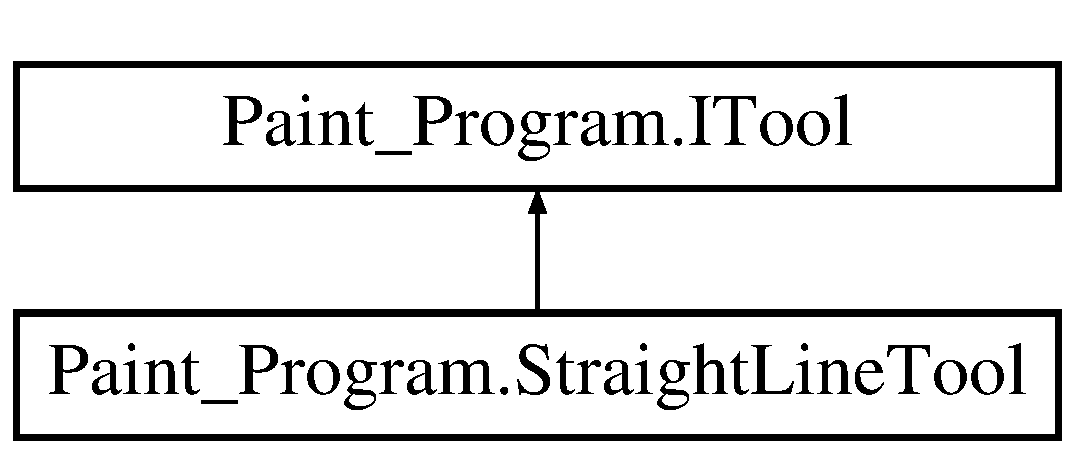
\includegraphics[height=2.000000cm]{class_paint___program_1_1_straight_line_tool}
\end{center}
\end{figure}
\subsection*{Public Member Functions}
\begin{DoxyCompactItemize}
\item 
\mbox{\hyperlink{class_paint___program_1_1_straight_line_tool_a4e09ab9bf0ef819ed906bfe82d9b76cf}{Straight\+Line\+Tool}} ()
\item 
void \mbox{\hyperlink{class_paint___program_1_1_straight_line_tool_a4c3cce5f1141100f04ed3a653d6936a1}{Init}} ()
\item 
string \mbox{\hyperlink{class_paint___program_1_1_straight_line_tool_ae260a0f50ea86b9ae9cceb36d1093057}{Get\+Tool\+Icon\+Path}} ()
\item 
void \mbox{\hyperlink{class_paint___program_1_1_straight_line_tool_a75f5c2ed8c11fef038f458324e1213f2}{On\+Mouse\+Down}} (object sender, Mouse\+Event\+Args e)
\item 
void \mbox{\hyperlink{class_paint___program_1_1_straight_line_tool_ad76feea781f953b41a22a940b1f12716}{On\+Mouse\+Move}} (object sender, Mouse\+Event\+Args e)
\item 
void \mbox{\hyperlink{class_paint___program_1_1_straight_line_tool_ab823dd700a2a92df78fe73b25c129c14}{On\+Mouse\+Up}} (object sender, Mouse\+Event\+Args e)
\item 
bool \mbox{\hyperlink{class_paint___program_1_1_straight_line_tool_aa4fa3f224adf151dd9dbbb97282cc989}{is\+Initalized}} ()
\item 
Bitmap \mbox{\hyperlink{class_paint___program_1_1_straight_line_tool_adb914fa4551bfee82d074838032d030b}{Get\+Tool\+Layer}} ()
\item 
bool \mbox{\hyperlink{class_paint___program_1_1_straight_line_tool_a27d923f2b23fbfa5e630af6d43c5e613}{Requires\+Layer\+Data}} ()
\item 
void \mbox{\hyperlink{class_paint___program_1_1_straight_line_tool_aaf03af3c789ac775fef1336c81c11a34}{Set\+Layer\+Data}} (Bitmap bit)
\item 
string \mbox{\hyperlink{class_paint___program_1_1_straight_line_tool_a1052069a81f2ba116bb27b3346b4030f}{Get\+Tool\+Tip}} ()
\item 
void \mbox{\hyperlink{class_paint___program_1_1_straight_line_tool_a42d3d814c74e317160779fbe9df3531b}{Update\+Interface\+Layer}} ()
\end{DoxyCompactItemize}
\subsection*{Private Member Functions}
\begin{DoxyCompactItemize}
\item 
void \mbox{\hyperlink{class_paint___program_1_1_straight_line_tool_a8069ecade0457152cb37ee7ea308f72d}{update\+Brush}} ()
\end{DoxyCompactItemize}
\subsection*{Private Attributes}
\begin{DoxyCompactItemize}
\item 
Graphics \mbox{\hyperlink{class_paint___program_1_1_straight_line_tool_a53a533731323ed3ffccce9c5b15e9918}{graphics}}
\item 
int \mbox{\hyperlink{class_paint___program_1_1_straight_line_tool_a5028852803a8d10f33cce71589b30a2c}{width}}
\item 
int \mbox{\hyperlink{class_paint___program_1_1_straight_line_tool_ac007cc9dcf0627d4f2c2da052c474147}{height}}
\item 
bool \mbox{\hyperlink{class_paint___program_1_1_straight_line_tool_a9f2f208b0bb6fd29b50f61390ba09bd1}{b\+Mouse\+Down}}
\item 
bool \mbox{\hyperlink{class_paint___program_1_1_straight_line_tool_a154b1cbdbf670e351aa6ed3b038ab149}{b\+Init}}
\item 
Point \mbox{\hyperlink{class_paint___program_1_1_straight_line_tool_a596c7efe86fcedf508afa1bcbc339aad}{p\+Old}}
\item 
Point \mbox{\hyperlink{class_paint___program_1_1_straight_line_tool_ad1bf03a5aff488c8668389bd74f50f66}{p\+New}}
\item 
Pen \mbox{\hyperlink{class_paint___program_1_1_straight_line_tool_aa54a4ef4085b40fd4892d1605dc136a9}{pen}}
\item 
Color \mbox{\hyperlink{class_paint___program_1_1_straight_line_tool_acdde166c5368a662c45af2d92a8a4ea5}{primary\+Color}}
\item 
Color \mbox{\hyperlink{class_paint___program_1_1_straight_line_tool_adf26467b59d71c4f15653a7fbafe348e}{secondary\+Color}}
\end{DoxyCompactItemize}


\subsection{Constructor \& Destructor Documentation}
\mbox{\Hypertarget{class_paint___program_1_1_straight_line_tool_a4e09ab9bf0ef819ed906bfe82d9b76cf}\label{class_paint___program_1_1_straight_line_tool_a4e09ab9bf0ef819ed906bfe82d9b76cf}} 
\index{Paint\+\_\+\+Program\+::\+Straight\+Line\+Tool@{Paint\+\_\+\+Program\+::\+Straight\+Line\+Tool}!Straight\+Line\+Tool@{Straight\+Line\+Tool}}
\index{Straight\+Line\+Tool@{Straight\+Line\+Tool}!Paint\+\_\+\+Program\+::\+Straight\+Line\+Tool@{Paint\+\_\+\+Program\+::\+Straight\+Line\+Tool}}
\subsubsection{\texorpdfstring{Straight\+Line\+Tool()}{StraightLineTool()}}
{\footnotesize\ttfamily Paint\+\_\+\+Program.\+Straight\+Line\+Tool.\+Straight\+Line\+Tool (\begin{DoxyParamCaption}{ }\end{DoxyParamCaption})\hspace{0.3cm}{\ttfamily [inline]}}



\subsection{Member Function Documentation}
\mbox{\Hypertarget{class_paint___program_1_1_straight_line_tool_ae260a0f50ea86b9ae9cceb36d1093057}\label{class_paint___program_1_1_straight_line_tool_ae260a0f50ea86b9ae9cceb36d1093057}} 
\index{Paint\+\_\+\+Program\+::\+Straight\+Line\+Tool@{Paint\+\_\+\+Program\+::\+Straight\+Line\+Tool}!Get\+Tool\+Icon\+Path@{Get\+Tool\+Icon\+Path}}
\index{Get\+Tool\+Icon\+Path@{Get\+Tool\+Icon\+Path}!Paint\+\_\+\+Program\+::\+Straight\+Line\+Tool@{Paint\+\_\+\+Program\+::\+Straight\+Line\+Tool}}
\subsubsection{\texorpdfstring{Get\+Tool\+Icon\+Path()}{GetToolIconPath()}}
{\footnotesize\ttfamily string Paint\+\_\+\+Program.\+Straight\+Line\+Tool.\+Get\+Tool\+Icon\+Path (\begin{DoxyParamCaption}{ }\end{DoxyParamCaption})\hspace{0.3cm}{\ttfamily [inline]}}



Implements \mbox{\hyperlink{interface_paint___program_1_1_i_tool_aa057d2f99c59d7bec0215dcad2da1b72}{Paint\+\_\+\+Program.\+I\+Tool}}.

\mbox{\Hypertarget{class_paint___program_1_1_straight_line_tool_adb914fa4551bfee82d074838032d030b}\label{class_paint___program_1_1_straight_line_tool_adb914fa4551bfee82d074838032d030b}} 
\index{Paint\+\_\+\+Program\+::\+Straight\+Line\+Tool@{Paint\+\_\+\+Program\+::\+Straight\+Line\+Tool}!Get\+Tool\+Layer@{Get\+Tool\+Layer}}
\index{Get\+Tool\+Layer@{Get\+Tool\+Layer}!Paint\+\_\+\+Program\+::\+Straight\+Line\+Tool@{Paint\+\_\+\+Program\+::\+Straight\+Line\+Tool}}
\subsubsection{\texorpdfstring{Get\+Tool\+Layer()}{GetToolLayer()}}
{\footnotesize\ttfamily Bitmap Paint\+\_\+\+Program.\+Straight\+Line\+Tool.\+Get\+Tool\+Layer (\begin{DoxyParamCaption}{ }\end{DoxyParamCaption})\hspace{0.3cm}{\ttfamily [inline]}}



Implements \mbox{\hyperlink{interface_paint___program_1_1_i_tool_a9b057905515f42a988c166a6a40318e0}{Paint\+\_\+\+Program.\+I\+Tool}}.

\mbox{\Hypertarget{class_paint___program_1_1_straight_line_tool_a1052069a81f2ba116bb27b3346b4030f}\label{class_paint___program_1_1_straight_line_tool_a1052069a81f2ba116bb27b3346b4030f}} 
\index{Paint\+\_\+\+Program\+::\+Straight\+Line\+Tool@{Paint\+\_\+\+Program\+::\+Straight\+Line\+Tool}!Get\+Tool\+Tip@{Get\+Tool\+Tip}}
\index{Get\+Tool\+Tip@{Get\+Tool\+Tip}!Paint\+\_\+\+Program\+::\+Straight\+Line\+Tool@{Paint\+\_\+\+Program\+::\+Straight\+Line\+Tool}}
\subsubsection{\texorpdfstring{Get\+Tool\+Tip()}{GetToolTip()}}
{\footnotesize\ttfamily string Paint\+\_\+\+Program.\+Straight\+Line\+Tool.\+Get\+Tool\+Tip (\begin{DoxyParamCaption}{ }\end{DoxyParamCaption})\hspace{0.3cm}{\ttfamily [inline]}}



Implements \mbox{\hyperlink{interface_paint___program_1_1_i_tool_ac11f1591587144b6e74f5767bbf1df56}{Paint\+\_\+\+Program.\+I\+Tool}}.

\mbox{\Hypertarget{class_paint___program_1_1_straight_line_tool_a4c3cce5f1141100f04ed3a653d6936a1}\label{class_paint___program_1_1_straight_line_tool_a4c3cce5f1141100f04ed3a653d6936a1}} 
\index{Paint\+\_\+\+Program\+::\+Straight\+Line\+Tool@{Paint\+\_\+\+Program\+::\+Straight\+Line\+Tool}!Init@{Init}}
\index{Init@{Init}!Paint\+\_\+\+Program\+::\+Straight\+Line\+Tool@{Paint\+\_\+\+Program\+::\+Straight\+Line\+Tool}}
\subsubsection{\texorpdfstring{Init()}{Init()}}
{\footnotesize\ttfamily void Paint\+\_\+\+Program.\+Straight\+Line\+Tool.\+Init (\begin{DoxyParamCaption}{ }\end{DoxyParamCaption})\hspace{0.3cm}{\ttfamily [inline]}}



Implements \mbox{\hyperlink{interface_paint___program_1_1_i_tool_af823123a30fbda34e24e907243241046}{Paint\+\_\+\+Program.\+I\+Tool}}.

\mbox{\Hypertarget{class_paint___program_1_1_straight_line_tool_aa4fa3f224adf151dd9dbbb97282cc989}\label{class_paint___program_1_1_straight_line_tool_aa4fa3f224adf151dd9dbbb97282cc989}} 
\index{Paint\+\_\+\+Program\+::\+Straight\+Line\+Tool@{Paint\+\_\+\+Program\+::\+Straight\+Line\+Tool}!is\+Initalized@{is\+Initalized}}
\index{is\+Initalized@{is\+Initalized}!Paint\+\_\+\+Program\+::\+Straight\+Line\+Tool@{Paint\+\_\+\+Program\+::\+Straight\+Line\+Tool}}
\subsubsection{\texorpdfstring{is\+Initalized()}{isInitalized()}}
{\footnotesize\ttfamily bool Paint\+\_\+\+Program.\+Straight\+Line\+Tool.\+is\+Initalized (\begin{DoxyParamCaption}{ }\end{DoxyParamCaption})\hspace{0.3cm}{\ttfamily [inline]}}



Implements \mbox{\hyperlink{interface_paint___program_1_1_i_tool_a951b844bcbf47a6c306104fa86be7a5d}{Paint\+\_\+\+Program.\+I\+Tool}}.

\mbox{\Hypertarget{class_paint___program_1_1_straight_line_tool_a75f5c2ed8c11fef038f458324e1213f2}\label{class_paint___program_1_1_straight_line_tool_a75f5c2ed8c11fef038f458324e1213f2}} 
\index{Paint\+\_\+\+Program\+::\+Straight\+Line\+Tool@{Paint\+\_\+\+Program\+::\+Straight\+Line\+Tool}!On\+Mouse\+Down@{On\+Mouse\+Down}}
\index{On\+Mouse\+Down@{On\+Mouse\+Down}!Paint\+\_\+\+Program\+::\+Straight\+Line\+Tool@{Paint\+\_\+\+Program\+::\+Straight\+Line\+Tool}}
\subsubsection{\texorpdfstring{On\+Mouse\+Down()}{OnMouseDown()}}
{\footnotesize\ttfamily void Paint\+\_\+\+Program.\+Straight\+Line\+Tool.\+On\+Mouse\+Down (\begin{DoxyParamCaption}\item[{object}]{sender,  }\item[{Mouse\+Event\+Args}]{e }\end{DoxyParamCaption})\hspace{0.3cm}{\ttfamily [inline]}}



Implements \mbox{\hyperlink{interface_paint___program_1_1_i_tool_a73d8797f4f2b1e0d8efe8aadcd44e840}{Paint\+\_\+\+Program.\+I\+Tool}}.

\mbox{\Hypertarget{class_paint___program_1_1_straight_line_tool_ad76feea781f953b41a22a940b1f12716}\label{class_paint___program_1_1_straight_line_tool_ad76feea781f953b41a22a940b1f12716}} 
\index{Paint\+\_\+\+Program\+::\+Straight\+Line\+Tool@{Paint\+\_\+\+Program\+::\+Straight\+Line\+Tool}!On\+Mouse\+Move@{On\+Mouse\+Move}}
\index{On\+Mouse\+Move@{On\+Mouse\+Move}!Paint\+\_\+\+Program\+::\+Straight\+Line\+Tool@{Paint\+\_\+\+Program\+::\+Straight\+Line\+Tool}}
\subsubsection{\texorpdfstring{On\+Mouse\+Move()}{OnMouseMove()}}
{\footnotesize\ttfamily void Paint\+\_\+\+Program.\+Straight\+Line\+Tool.\+On\+Mouse\+Move (\begin{DoxyParamCaption}\item[{object}]{sender,  }\item[{Mouse\+Event\+Args}]{e }\end{DoxyParamCaption})\hspace{0.3cm}{\ttfamily [inline]}}



Implements \mbox{\hyperlink{interface_paint___program_1_1_i_tool_a6a1cbe840b5cfc8a9b9463cc21590845}{Paint\+\_\+\+Program.\+I\+Tool}}.

\mbox{\Hypertarget{class_paint___program_1_1_straight_line_tool_ab823dd700a2a92df78fe73b25c129c14}\label{class_paint___program_1_1_straight_line_tool_ab823dd700a2a92df78fe73b25c129c14}} 
\index{Paint\+\_\+\+Program\+::\+Straight\+Line\+Tool@{Paint\+\_\+\+Program\+::\+Straight\+Line\+Tool}!On\+Mouse\+Up@{On\+Mouse\+Up}}
\index{On\+Mouse\+Up@{On\+Mouse\+Up}!Paint\+\_\+\+Program\+::\+Straight\+Line\+Tool@{Paint\+\_\+\+Program\+::\+Straight\+Line\+Tool}}
\subsubsection{\texorpdfstring{On\+Mouse\+Up()}{OnMouseUp()}}
{\footnotesize\ttfamily void Paint\+\_\+\+Program.\+Straight\+Line\+Tool.\+On\+Mouse\+Up (\begin{DoxyParamCaption}\item[{object}]{sender,  }\item[{Mouse\+Event\+Args}]{e }\end{DoxyParamCaption})\hspace{0.3cm}{\ttfamily [inline]}}



Implements \mbox{\hyperlink{interface_paint___program_1_1_i_tool_a47984c2879213022f1684c07f7bba73e}{Paint\+\_\+\+Program.\+I\+Tool}}.

\mbox{\Hypertarget{class_paint___program_1_1_straight_line_tool_a27d923f2b23fbfa5e630af6d43c5e613}\label{class_paint___program_1_1_straight_line_tool_a27d923f2b23fbfa5e630af6d43c5e613}} 
\index{Paint\+\_\+\+Program\+::\+Straight\+Line\+Tool@{Paint\+\_\+\+Program\+::\+Straight\+Line\+Tool}!Requires\+Layer\+Data@{Requires\+Layer\+Data}}
\index{Requires\+Layer\+Data@{Requires\+Layer\+Data}!Paint\+\_\+\+Program\+::\+Straight\+Line\+Tool@{Paint\+\_\+\+Program\+::\+Straight\+Line\+Tool}}
\subsubsection{\texorpdfstring{Requires\+Layer\+Data()}{RequiresLayerData()}}
{\footnotesize\ttfamily bool Paint\+\_\+\+Program.\+Straight\+Line\+Tool.\+Requires\+Layer\+Data (\begin{DoxyParamCaption}{ }\end{DoxyParamCaption})\hspace{0.3cm}{\ttfamily [inline]}}



Implements \mbox{\hyperlink{interface_paint___program_1_1_i_tool_a6d45b6c48da8130ae41db3a66cdaef9a}{Paint\+\_\+\+Program.\+I\+Tool}}.

\mbox{\Hypertarget{class_paint___program_1_1_straight_line_tool_aaf03af3c789ac775fef1336c81c11a34}\label{class_paint___program_1_1_straight_line_tool_aaf03af3c789ac775fef1336c81c11a34}} 
\index{Paint\+\_\+\+Program\+::\+Straight\+Line\+Tool@{Paint\+\_\+\+Program\+::\+Straight\+Line\+Tool}!Set\+Layer\+Data@{Set\+Layer\+Data}}
\index{Set\+Layer\+Data@{Set\+Layer\+Data}!Paint\+\_\+\+Program\+::\+Straight\+Line\+Tool@{Paint\+\_\+\+Program\+::\+Straight\+Line\+Tool}}
\subsubsection{\texorpdfstring{Set\+Layer\+Data()}{SetLayerData()}}
{\footnotesize\ttfamily void Paint\+\_\+\+Program.\+Straight\+Line\+Tool.\+Set\+Layer\+Data (\begin{DoxyParamCaption}\item[{Bitmap}]{bit }\end{DoxyParamCaption})\hspace{0.3cm}{\ttfamily [inline]}}



Implements \mbox{\hyperlink{interface_paint___program_1_1_i_tool_a2d3e63715dfe04075d27dacf367d1633}{Paint\+\_\+\+Program.\+I\+Tool}}.

\mbox{\Hypertarget{class_paint___program_1_1_straight_line_tool_a8069ecade0457152cb37ee7ea308f72d}\label{class_paint___program_1_1_straight_line_tool_a8069ecade0457152cb37ee7ea308f72d}} 
\index{Paint\+\_\+\+Program\+::\+Straight\+Line\+Tool@{Paint\+\_\+\+Program\+::\+Straight\+Line\+Tool}!update\+Brush@{update\+Brush}}
\index{update\+Brush@{update\+Brush}!Paint\+\_\+\+Program\+::\+Straight\+Line\+Tool@{Paint\+\_\+\+Program\+::\+Straight\+Line\+Tool}}
\subsubsection{\texorpdfstring{update\+Brush()}{updateBrush()}}
{\footnotesize\ttfamily void Paint\+\_\+\+Program.\+Straight\+Line\+Tool.\+update\+Brush (\begin{DoxyParamCaption}{ }\end{DoxyParamCaption})\hspace{0.3cm}{\ttfamily [inline]}, {\ttfamily [private]}}

\mbox{\Hypertarget{class_paint___program_1_1_straight_line_tool_a42d3d814c74e317160779fbe9df3531b}\label{class_paint___program_1_1_straight_line_tool_a42d3d814c74e317160779fbe9df3531b}} 
\index{Paint\+\_\+\+Program\+::\+Straight\+Line\+Tool@{Paint\+\_\+\+Program\+::\+Straight\+Line\+Tool}!Update\+Interface\+Layer@{Update\+Interface\+Layer}}
\index{Update\+Interface\+Layer@{Update\+Interface\+Layer}!Paint\+\_\+\+Program\+::\+Straight\+Line\+Tool@{Paint\+\_\+\+Program\+::\+Straight\+Line\+Tool}}
\subsubsection{\texorpdfstring{Update\+Interface\+Layer()}{UpdateInterfaceLayer()}}
{\footnotesize\ttfamily void Paint\+\_\+\+Program.\+Straight\+Line\+Tool.\+Update\+Interface\+Layer (\begin{DoxyParamCaption}{ }\end{DoxyParamCaption})\hspace{0.3cm}{\ttfamily [inline]}}



Implements \mbox{\hyperlink{interface_paint___program_1_1_i_tool_a36db75d29e88dfd739f658633c40e955}{Paint\+\_\+\+Program.\+I\+Tool}}.



\subsection{Member Data Documentation}
\mbox{\Hypertarget{class_paint___program_1_1_straight_line_tool_a154b1cbdbf670e351aa6ed3b038ab149}\label{class_paint___program_1_1_straight_line_tool_a154b1cbdbf670e351aa6ed3b038ab149}} 
\index{Paint\+\_\+\+Program\+::\+Straight\+Line\+Tool@{Paint\+\_\+\+Program\+::\+Straight\+Line\+Tool}!b\+Init@{b\+Init}}
\index{b\+Init@{b\+Init}!Paint\+\_\+\+Program\+::\+Straight\+Line\+Tool@{Paint\+\_\+\+Program\+::\+Straight\+Line\+Tool}}
\subsubsection{\texorpdfstring{b\+Init}{bInit}}
{\footnotesize\ttfamily bool Paint\+\_\+\+Program.\+Straight\+Line\+Tool.\+b\+Init\hspace{0.3cm}{\ttfamily [private]}}

\mbox{\Hypertarget{class_paint___program_1_1_straight_line_tool_a9f2f208b0bb6fd29b50f61390ba09bd1}\label{class_paint___program_1_1_straight_line_tool_a9f2f208b0bb6fd29b50f61390ba09bd1}} 
\index{Paint\+\_\+\+Program\+::\+Straight\+Line\+Tool@{Paint\+\_\+\+Program\+::\+Straight\+Line\+Tool}!b\+Mouse\+Down@{b\+Mouse\+Down}}
\index{b\+Mouse\+Down@{b\+Mouse\+Down}!Paint\+\_\+\+Program\+::\+Straight\+Line\+Tool@{Paint\+\_\+\+Program\+::\+Straight\+Line\+Tool}}
\subsubsection{\texorpdfstring{b\+Mouse\+Down}{bMouseDown}}
{\footnotesize\ttfamily bool Paint\+\_\+\+Program.\+Straight\+Line\+Tool.\+b\+Mouse\+Down\hspace{0.3cm}{\ttfamily [private]}}

\mbox{\Hypertarget{class_paint___program_1_1_straight_line_tool_a53a533731323ed3ffccce9c5b15e9918}\label{class_paint___program_1_1_straight_line_tool_a53a533731323ed3ffccce9c5b15e9918}} 
\index{Paint\+\_\+\+Program\+::\+Straight\+Line\+Tool@{Paint\+\_\+\+Program\+::\+Straight\+Line\+Tool}!graphics@{graphics}}
\index{graphics@{graphics}!Paint\+\_\+\+Program\+::\+Straight\+Line\+Tool@{Paint\+\_\+\+Program\+::\+Straight\+Line\+Tool}}
\subsubsection{\texorpdfstring{graphics}{graphics}}
{\footnotesize\ttfamily Graphics Paint\+\_\+\+Program.\+Straight\+Line\+Tool.\+graphics\hspace{0.3cm}{\ttfamily [private]}}

\mbox{\Hypertarget{class_paint___program_1_1_straight_line_tool_ac007cc9dcf0627d4f2c2da052c474147}\label{class_paint___program_1_1_straight_line_tool_ac007cc9dcf0627d4f2c2da052c474147}} 
\index{Paint\+\_\+\+Program\+::\+Straight\+Line\+Tool@{Paint\+\_\+\+Program\+::\+Straight\+Line\+Tool}!height@{height}}
\index{height@{height}!Paint\+\_\+\+Program\+::\+Straight\+Line\+Tool@{Paint\+\_\+\+Program\+::\+Straight\+Line\+Tool}}
\subsubsection{\texorpdfstring{height}{height}}
{\footnotesize\ttfamily int Paint\+\_\+\+Program.\+Straight\+Line\+Tool.\+height\hspace{0.3cm}{\ttfamily [private]}}

\mbox{\Hypertarget{class_paint___program_1_1_straight_line_tool_aa54a4ef4085b40fd4892d1605dc136a9}\label{class_paint___program_1_1_straight_line_tool_aa54a4ef4085b40fd4892d1605dc136a9}} 
\index{Paint\+\_\+\+Program\+::\+Straight\+Line\+Tool@{Paint\+\_\+\+Program\+::\+Straight\+Line\+Tool}!pen@{pen}}
\index{pen@{pen}!Paint\+\_\+\+Program\+::\+Straight\+Line\+Tool@{Paint\+\_\+\+Program\+::\+Straight\+Line\+Tool}}
\subsubsection{\texorpdfstring{pen}{pen}}
{\footnotesize\ttfamily Pen Paint\+\_\+\+Program.\+Straight\+Line\+Tool.\+pen\hspace{0.3cm}{\ttfamily [private]}}

\mbox{\Hypertarget{class_paint___program_1_1_straight_line_tool_ad1bf03a5aff488c8668389bd74f50f66}\label{class_paint___program_1_1_straight_line_tool_ad1bf03a5aff488c8668389bd74f50f66}} 
\index{Paint\+\_\+\+Program\+::\+Straight\+Line\+Tool@{Paint\+\_\+\+Program\+::\+Straight\+Line\+Tool}!p\+New@{p\+New}}
\index{p\+New@{p\+New}!Paint\+\_\+\+Program\+::\+Straight\+Line\+Tool@{Paint\+\_\+\+Program\+::\+Straight\+Line\+Tool}}
\subsubsection{\texorpdfstring{p\+New}{pNew}}
{\footnotesize\ttfamily Point Paint\+\_\+\+Program.\+Straight\+Line\+Tool.\+p\+New\hspace{0.3cm}{\ttfamily [private]}}

\mbox{\Hypertarget{class_paint___program_1_1_straight_line_tool_a596c7efe86fcedf508afa1bcbc339aad}\label{class_paint___program_1_1_straight_line_tool_a596c7efe86fcedf508afa1bcbc339aad}} 
\index{Paint\+\_\+\+Program\+::\+Straight\+Line\+Tool@{Paint\+\_\+\+Program\+::\+Straight\+Line\+Tool}!p\+Old@{p\+Old}}
\index{p\+Old@{p\+Old}!Paint\+\_\+\+Program\+::\+Straight\+Line\+Tool@{Paint\+\_\+\+Program\+::\+Straight\+Line\+Tool}}
\subsubsection{\texorpdfstring{p\+Old}{pOld}}
{\footnotesize\ttfamily Point Paint\+\_\+\+Program.\+Straight\+Line\+Tool.\+p\+Old\hspace{0.3cm}{\ttfamily [private]}}

\mbox{\Hypertarget{class_paint___program_1_1_straight_line_tool_acdde166c5368a662c45af2d92a8a4ea5}\label{class_paint___program_1_1_straight_line_tool_acdde166c5368a662c45af2d92a8a4ea5}} 
\index{Paint\+\_\+\+Program\+::\+Straight\+Line\+Tool@{Paint\+\_\+\+Program\+::\+Straight\+Line\+Tool}!primary\+Color@{primary\+Color}}
\index{primary\+Color@{primary\+Color}!Paint\+\_\+\+Program\+::\+Straight\+Line\+Tool@{Paint\+\_\+\+Program\+::\+Straight\+Line\+Tool}}
\subsubsection{\texorpdfstring{primary\+Color}{primaryColor}}
{\footnotesize\ttfamily Color Paint\+\_\+\+Program.\+Straight\+Line\+Tool.\+primary\+Color\hspace{0.3cm}{\ttfamily [private]}}

\mbox{\Hypertarget{class_paint___program_1_1_straight_line_tool_adf26467b59d71c4f15653a7fbafe348e}\label{class_paint___program_1_1_straight_line_tool_adf26467b59d71c4f15653a7fbafe348e}} 
\index{Paint\+\_\+\+Program\+::\+Straight\+Line\+Tool@{Paint\+\_\+\+Program\+::\+Straight\+Line\+Tool}!secondary\+Color@{secondary\+Color}}
\index{secondary\+Color@{secondary\+Color}!Paint\+\_\+\+Program\+::\+Straight\+Line\+Tool@{Paint\+\_\+\+Program\+::\+Straight\+Line\+Tool}}
\subsubsection{\texorpdfstring{secondary\+Color}{secondaryColor}}
{\footnotesize\ttfamily Color Paint\+\_\+\+Program.\+Straight\+Line\+Tool.\+secondary\+Color\hspace{0.3cm}{\ttfamily [private]}}

\mbox{\Hypertarget{class_paint___program_1_1_straight_line_tool_a5028852803a8d10f33cce71589b30a2c}\label{class_paint___program_1_1_straight_line_tool_a5028852803a8d10f33cce71589b30a2c}} 
\index{Paint\+\_\+\+Program\+::\+Straight\+Line\+Tool@{Paint\+\_\+\+Program\+::\+Straight\+Line\+Tool}!width@{width}}
\index{width@{width}!Paint\+\_\+\+Program\+::\+Straight\+Line\+Tool@{Paint\+\_\+\+Program\+::\+Straight\+Line\+Tool}}
\subsubsection{\texorpdfstring{width}{width}}
{\footnotesize\ttfamily int Paint\+\_\+\+Program.\+Straight\+Line\+Tool.\+width\hspace{0.3cm}{\ttfamily [private]}}



The documentation for this class was generated from the following file\+:\begin{DoxyCompactItemize}
\item 
Paint Program/\mbox{\hyperlink{_straight_line_tool_8cs}{Straight\+Line\+Tool.\+cs}}\end{DoxyCompactItemize}

\hypertarget{class_paint___program_1_1_tablet_info}{}\section{Paint\+\_\+\+Program.\+Tablet\+Info Class Reference}
\label{class_paint___program_1_1_tablet_info}\index{Paint\+\_\+\+Program.\+Tablet\+Info@{Paint\+\_\+\+Program.\+Tablet\+Info}}
\subsection*{Public Member Functions}
\begin{DoxyCompactItemize}
\item 
\mbox{\hyperlink{class_paint___program_1_1_tablet_info_afc7015701d66e276d81ffb40fb22e381}{Tablet\+Info}} (Event\+Handler$<$ \mbox{\hyperlink{class_wintab_d_n_1_1_message_received_event_args}{Message\+Received\+Event\+Args}} $>$ handler)
\item 
\mbox{\hyperlink{class_wintab_d_n_1_1_c_wintab_data}{C\+Wintab\+Data}} \mbox{\hyperlink{class_paint___program_1_1_tablet_info_ab9818599347fcfbc04c65e173ffe53a3}{get\+Wintab\+Data}} ()
\item 
U\+Int32 \mbox{\hyperlink{class_paint___program_1_1_tablet_info_a934c6f9d86beb999e083eb871dc59cc6}{get\+Max\+Packets}} ()
\end{DoxyCompactItemize}
\subsection*{Private Member Functions}
\begin{DoxyCompactItemize}
\item 
void \mbox{\hyperlink{class_paint___program_1_1_tablet_info_a57837c298e04350bc3611b0ed093ee8c}{Test\+\_\+\+Is\+Wintab\+Available}} ()
\item 
void \mbox{\hyperlink{class_paint___program_1_1_tablet_info_a7fc19fda1a1444bdc4229a10c7018599}{Test\+\_\+\+Get\+Device\+Info}} ()
\item 
void \mbox{\hyperlink{class_paint___program_1_1_tablet_info_a508f66e245bce37ffd182f0ba180bfeb}{Test\+\_\+\+Get\+Default\+Digitizing\+Context}} ()
\item 
void \mbox{\hyperlink{class_paint___program_1_1_tablet_info_a6dfaef8dbc743bfbffab4a2cf3f13087}{Test\+\_\+\+Get\+Default\+System\+Context}} ()
\item 
void \mbox{\hyperlink{class_paint___program_1_1_tablet_info_ac5bb83e6ba49dfb4a6522d67e5553819}{Test\+\_\+\+Get\+Default\+Device\+Index}} ()
\item 
void \mbox{\hyperlink{class_paint___program_1_1_tablet_info_a8a9237e85de0f55296d5f0098eec9ec8}{Test\+\_\+\+Get\+Device\+Axis}} ()
\item 
void \mbox{\hyperlink{class_paint___program_1_1_tablet_info_ab4f7f782ed10c11ee9ae2c574ba33ca0}{Test\+\_\+\+Get\+Device\+Orientation}} ()
\item 
void \mbox{\hyperlink{class_paint___program_1_1_tablet_info_ad9df50108fcb977ee9e1e36b9e4c0220}{Test\+\_\+\+Get\+Device\+Rotation}} ()
\item 
U\+Int32 \mbox{\hyperlink{class_paint___program_1_1_tablet_info_ae53a72d08d3fcc6891f5e39d94f91b97}{Test\+\_\+\+Get\+Number\+Of\+Devices}} ()
\item 
void \mbox{\hyperlink{class_paint___program_1_1_tablet_info_a02866892ffb797cdc49c030bd72cbac1}{Test\+\_\+\+Is\+Stylus\+Active}} ()
\item 
void \mbox{\hyperlink{class_paint___program_1_1_tablet_info_aab8b9141d7d24e97ba6a4cb71af0f481}{Test\+\_\+\+Get\+Stylus\+Name}} ()
\item 
void \mbox{\hyperlink{class_paint___program_1_1_tablet_info_a065e2f91a52ee65c40da83cefd33b796}{Test\+\_\+\+Get\+Extension\+Mask}} ()
\item 
void \mbox{\hyperlink{class_paint___program_1_1_tablet_info_a7856382bc542b2a4f8c5bebda8dc588a}{Test\+\_\+\+Max\+Pressure}} ()
\item 
void \mbox{\hyperlink{class_paint___program_1_1_tablet_info_ae3eaec5febf23138a724e6b5d94d2e9a}{Init\+Data\+Capture}} (Event\+Handler$<$ \mbox{\hyperlink{class_wintab_d_n_1_1_message_received_event_args}{Message\+Received\+Event\+Args}} $>$ handler, int ctx\+Width\+\_\+I=\mbox{\hyperlink{class_paint___program_1_1_tablet_info_aec96087301274b16e37ad97d9d86f2a8}{m\+\_\+\+T\+A\+B\+E\+X\+TX}}, int ctx\+Height\+\_\+I=\mbox{\hyperlink{class_paint___program_1_1_tablet_info_a694255f1b42334dcd3c05f6ff9b0ff6d}{m\+\_\+\+T\+A\+B\+E\+X\+TY}}, bool ctrl\+Sys\+Cursor\+\_\+I=true)
\item 
\mbox{\hyperlink{class_wintab_d_n_1_1_c_wintab_context}{C\+Wintab\+Context}} \mbox{\hyperlink{class_paint___program_1_1_tablet_info_ab02b5950a6b9f9c29104a2d68d2ba26b}{Open\+Test\+System\+Context}} (int width\+\_\+I=\mbox{\hyperlink{class_paint___program_1_1_tablet_info_aec96087301274b16e37ad97d9d86f2a8}{m\+\_\+\+T\+A\+B\+E\+X\+TX}}, int height\+\_\+I=\mbox{\hyperlink{class_paint___program_1_1_tablet_info_a694255f1b42334dcd3c05f6ff9b0ff6d}{m\+\_\+\+T\+A\+B\+E\+X\+TY}}, bool ctrl\+Sys\+Cursor=true)
\item 
void \mbox{\hyperlink{class_paint___program_1_1_tablet_info_aa34192cb8b5aad8e9741543b8cafb217}{Set\+System\+Extents}} (ref \mbox{\hyperlink{class_wintab_d_n_1_1_c_wintab_context}{C\+Wintab\+Context}} log\+Context)
\item 
void \mbox{\hyperlink{class_paint___program_1_1_tablet_info_aff74e48af72f51c33129c437db898103}{Close\+Current\+Context}} ()
\end{DoxyCompactItemize}
\subsection*{Private Attributes}
\begin{DoxyCompactItemize}
\item 
\mbox{\hyperlink{class_wintab_d_n_1_1_c_wintab_context}{C\+Wintab\+Context}} \mbox{\hyperlink{class_paint___program_1_1_tablet_info_a1e7da115e188bc9294ab639f5f75e61b}{m\+\_\+log\+Context}} = null
\item 
\mbox{\hyperlink{class_wintab_d_n_1_1_c_wintab_data}{C\+Wintab\+Data}} \mbox{\hyperlink{class_paint___program_1_1_tablet_info_a7c514892b904d4d34d22791cd9047b82}{m\+\_\+wt\+Data}} = null
\item 
U\+Int32 \mbox{\hyperlink{class_paint___program_1_1_tablet_info_a70180b4d0d8ac8fe1cc200c20856a171}{m\+\_\+max\+Pkts}} = 1
\item 
Int32 \mbox{\hyperlink{class_paint___program_1_1_tablet_info_a8a6421486fbf0fc498b735e0de3290ee}{m\+\_\+pkX}} = 0
\item 
Int32 \mbox{\hyperlink{class_paint___program_1_1_tablet_info_a8c23e48316f05b16fb46c8eb4ebc6308}{m\+\_\+pkY}} = 0
\item 
U\+Int32 \mbox{\hyperlink{class_paint___program_1_1_tablet_info_a582fe5c923f467fbf898aeac0d7780dd}{m\+\_\+pressure}} = 0
\item 
U\+Int32 \mbox{\hyperlink{class_paint___program_1_1_tablet_info_af7b50d0820544e080adf02c24b309959}{m\+\_\+pk\+Time}} = 0
\item 
U\+Int32 \mbox{\hyperlink{class_paint___program_1_1_tablet_info_a8f8efea7a323142ae19efd50b02b859e}{m\+\_\+pk\+Time\+Last}} = 0
\item 
const Int32 \mbox{\hyperlink{class_paint___program_1_1_tablet_info_aec96087301274b16e37ad97d9d86f2a8}{m\+\_\+\+T\+A\+B\+E\+X\+TX}} = 10000
\item 
const Int32 \mbox{\hyperlink{class_paint___program_1_1_tablet_info_a694255f1b42334dcd3c05f6ff9b0ff6d}{m\+\_\+\+T\+A\+B\+E\+X\+TY}} = 10000
\end{DoxyCompactItemize}


\subsection{Constructor \& Destructor Documentation}
\mbox{\Hypertarget{class_paint___program_1_1_tablet_info_afc7015701d66e276d81ffb40fb22e381}\label{class_paint___program_1_1_tablet_info_afc7015701d66e276d81ffb40fb22e381}} 
\index{Paint\+\_\+\+Program\+::\+Tablet\+Info@{Paint\+\_\+\+Program\+::\+Tablet\+Info}!Tablet\+Info@{Tablet\+Info}}
\index{Tablet\+Info@{Tablet\+Info}!Paint\+\_\+\+Program\+::\+Tablet\+Info@{Paint\+\_\+\+Program\+::\+Tablet\+Info}}
\subsubsection{\texorpdfstring{Tablet\+Info()}{TabletInfo()}}
{\footnotesize\ttfamily Paint\+\_\+\+Program.\+Tablet\+Info.\+Tablet\+Info (\begin{DoxyParamCaption}\item[{Event\+Handler$<$ \mbox{\hyperlink{class_wintab_d_n_1_1_message_received_event_args}{Message\+Received\+Event\+Args}} $>$}]{handler }\end{DoxyParamCaption})\hspace{0.3cm}{\ttfamily [inline]}}



\subsection{Member Function Documentation}
\mbox{\Hypertarget{class_paint___program_1_1_tablet_info_aff74e48af72f51c33129c437db898103}\label{class_paint___program_1_1_tablet_info_aff74e48af72f51c33129c437db898103}} 
\index{Paint\+\_\+\+Program\+::\+Tablet\+Info@{Paint\+\_\+\+Program\+::\+Tablet\+Info}!Close\+Current\+Context@{Close\+Current\+Context}}
\index{Close\+Current\+Context@{Close\+Current\+Context}!Paint\+\_\+\+Program\+::\+Tablet\+Info@{Paint\+\_\+\+Program\+::\+Tablet\+Info}}
\subsubsection{\texorpdfstring{Close\+Current\+Context()}{CloseCurrentContext()}}
{\footnotesize\ttfamily void Paint\+\_\+\+Program.\+Tablet\+Info.\+Close\+Current\+Context (\begin{DoxyParamCaption}{ }\end{DoxyParamCaption})\hspace{0.3cm}{\ttfamily [inline]}, {\ttfamily [private]}}

\mbox{\Hypertarget{class_paint___program_1_1_tablet_info_a934c6f9d86beb999e083eb871dc59cc6}\label{class_paint___program_1_1_tablet_info_a934c6f9d86beb999e083eb871dc59cc6}} 
\index{Paint\+\_\+\+Program\+::\+Tablet\+Info@{Paint\+\_\+\+Program\+::\+Tablet\+Info}!get\+Max\+Packets@{get\+Max\+Packets}}
\index{get\+Max\+Packets@{get\+Max\+Packets}!Paint\+\_\+\+Program\+::\+Tablet\+Info@{Paint\+\_\+\+Program\+::\+Tablet\+Info}}
\subsubsection{\texorpdfstring{get\+Max\+Packets()}{getMaxPackets()}}
{\footnotesize\ttfamily U\+Int32 Paint\+\_\+\+Program.\+Tablet\+Info.\+get\+Max\+Packets (\begin{DoxyParamCaption}{ }\end{DoxyParamCaption})\hspace{0.3cm}{\ttfamily [inline]}}

\mbox{\Hypertarget{class_paint___program_1_1_tablet_info_ab9818599347fcfbc04c65e173ffe53a3}\label{class_paint___program_1_1_tablet_info_ab9818599347fcfbc04c65e173ffe53a3}} 
\index{Paint\+\_\+\+Program\+::\+Tablet\+Info@{Paint\+\_\+\+Program\+::\+Tablet\+Info}!get\+Wintab\+Data@{get\+Wintab\+Data}}
\index{get\+Wintab\+Data@{get\+Wintab\+Data}!Paint\+\_\+\+Program\+::\+Tablet\+Info@{Paint\+\_\+\+Program\+::\+Tablet\+Info}}
\subsubsection{\texorpdfstring{get\+Wintab\+Data()}{getWintabData()}}
{\footnotesize\ttfamily \mbox{\hyperlink{class_wintab_d_n_1_1_c_wintab_data}{C\+Wintab\+Data}} Paint\+\_\+\+Program.\+Tablet\+Info.\+get\+Wintab\+Data (\begin{DoxyParamCaption}{ }\end{DoxyParamCaption})\hspace{0.3cm}{\ttfamily [inline]}}

\mbox{\Hypertarget{class_paint___program_1_1_tablet_info_ae3eaec5febf23138a724e6b5d94d2e9a}\label{class_paint___program_1_1_tablet_info_ae3eaec5febf23138a724e6b5d94d2e9a}} 
\index{Paint\+\_\+\+Program\+::\+Tablet\+Info@{Paint\+\_\+\+Program\+::\+Tablet\+Info}!Init\+Data\+Capture@{Init\+Data\+Capture}}
\index{Init\+Data\+Capture@{Init\+Data\+Capture}!Paint\+\_\+\+Program\+::\+Tablet\+Info@{Paint\+\_\+\+Program\+::\+Tablet\+Info}}
\subsubsection{\texorpdfstring{Init\+Data\+Capture()}{InitDataCapture()}}
{\footnotesize\ttfamily void Paint\+\_\+\+Program.\+Tablet\+Info.\+Init\+Data\+Capture (\begin{DoxyParamCaption}\item[{Event\+Handler$<$ \mbox{\hyperlink{class_wintab_d_n_1_1_message_received_event_args}{Message\+Received\+Event\+Args}} $>$}]{handler,  }\item[{int}]{ctx\+Width\+\_\+I = {\ttfamily \mbox{\hyperlink{class_paint___program_1_1_tablet_info_aec96087301274b16e37ad97d9d86f2a8}{m\+\_\+\+T\+A\+B\+E\+X\+TX}}},  }\item[{int}]{ctx\+Height\+\_\+I = {\ttfamily \mbox{\hyperlink{class_paint___program_1_1_tablet_info_a694255f1b42334dcd3c05f6ff9b0ff6d}{m\+\_\+\+T\+A\+B\+E\+X\+TY}}},  }\item[{bool}]{ctrl\+Sys\+Cursor\+\_\+I = {\ttfamily true} }\end{DoxyParamCaption})\hspace{0.3cm}{\ttfamily [inline]}, {\ttfamily [private]}}

\mbox{\Hypertarget{class_paint___program_1_1_tablet_info_ab02b5950a6b9f9c29104a2d68d2ba26b}\label{class_paint___program_1_1_tablet_info_ab02b5950a6b9f9c29104a2d68d2ba26b}} 
\index{Paint\+\_\+\+Program\+::\+Tablet\+Info@{Paint\+\_\+\+Program\+::\+Tablet\+Info}!Open\+Test\+System\+Context@{Open\+Test\+System\+Context}}
\index{Open\+Test\+System\+Context@{Open\+Test\+System\+Context}!Paint\+\_\+\+Program\+::\+Tablet\+Info@{Paint\+\_\+\+Program\+::\+Tablet\+Info}}
\subsubsection{\texorpdfstring{Open\+Test\+System\+Context()}{OpenTestSystemContext()}}
{\footnotesize\ttfamily \mbox{\hyperlink{class_wintab_d_n_1_1_c_wintab_context}{C\+Wintab\+Context}} Paint\+\_\+\+Program.\+Tablet\+Info.\+Open\+Test\+System\+Context (\begin{DoxyParamCaption}\item[{int}]{width\+\_\+I = {\ttfamily \mbox{\hyperlink{class_paint___program_1_1_tablet_info_aec96087301274b16e37ad97d9d86f2a8}{m\+\_\+\+T\+A\+B\+E\+X\+TX}}},  }\item[{int}]{height\+\_\+I = {\ttfamily \mbox{\hyperlink{class_paint___program_1_1_tablet_info_a694255f1b42334dcd3c05f6ff9b0ff6d}{m\+\_\+\+T\+A\+B\+E\+X\+TY}}},  }\item[{bool}]{ctrl\+Sys\+Cursor = {\ttfamily true} }\end{DoxyParamCaption})\hspace{0.3cm}{\ttfamily [inline]}, {\ttfamily [private]}}

\mbox{\Hypertarget{class_paint___program_1_1_tablet_info_aa34192cb8b5aad8e9741543b8cafb217}\label{class_paint___program_1_1_tablet_info_aa34192cb8b5aad8e9741543b8cafb217}} 
\index{Paint\+\_\+\+Program\+::\+Tablet\+Info@{Paint\+\_\+\+Program\+::\+Tablet\+Info}!Set\+System\+Extents@{Set\+System\+Extents}}
\index{Set\+System\+Extents@{Set\+System\+Extents}!Paint\+\_\+\+Program\+::\+Tablet\+Info@{Paint\+\_\+\+Program\+::\+Tablet\+Info}}
\subsubsection{\texorpdfstring{Set\+System\+Extents()}{SetSystemExtents()}}
{\footnotesize\ttfamily void Paint\+\_\+\+Program.\+Tablet\+Info.\+Set\+System\+Extents (\begin{DoxyParamCaption}\item[{ref \mbox{\hyperlink{class_wintab_d_n_1_1_c_wintab_context}{C\+Wintab\+Context}}}]{log\+Context }\end{DoxyParamCaption})\hspace{0.3cm}{\ttfamily [inline]}, {\ttfamily [private]}}

\mbox{\Hypertarget{class_paint___program_1_1_tablet_info_ac5bb83e6ba49dfb4a6522d67e5553819}\label{class_paint___program_1_1_tablet_info_ac5bb83e6ba49dfb4a6522d67e5553819}} 
\index{Paint\+\_\+\+Program\+::\+Tablet\+Info@{Paint\+\_\+\+Program\+::\+Tablet\+Info}!Test\+\_\+\+Get\+Default\+Device\+Index@{Test\+\_\+\+Get\+Default\+Device\+Index}}
\index{Test\+\_\+\+Get\+Default\+Device\+Index@{Test\+\_\+\+Get\+Default\+Device\+Index}!Paint\+\_\+\+Program\+::\+Tablet\+Info@{Paint\+\_\+\+Program\+::\+Tablet\+Info}}
\subsubsection{\texorpdfstring{Test\+\_\+\+Get\+Default\+Device\+Index()}{Test\_GetDefaultDeviceIndex()}}
{\footnotesize\ttfamily void Paint\+\_\+\+Program.\+Tablet\+Info.\+Test\+\_\+\+Get\+Default\+Device\+Index (\begin{DoxyParamCaption}{ }\end{DoxyParamCaption})\hspace{0.3cm}{\ttfamily [inline]}, {\ttfamily [private]}}

\mbox{\Hypertarget{class_paint___program_1_1_tablet_info_a508f66e245bce37ffd182f0ba180bfeb}\label{class_paint___program_1_1_tablet_info_a508f66e245bce37ffd182f0ba180bfeb}} 
\index{Paint\+\_\+\+Program\+::\+Tablet\+Info@{Paint\+\_\+\+Program\+::\+Tablet\+Info}!Test\+\_\+\+Get\+Default\+Digitizing\+Context@{Test\+\_\+\+Get\+Default\+Digitizing\+Context}}
\index{Test\+\_\+\+Get\+Default\+Digitizing\+Context@{Test\+\_\+\+Get\+Default\+Digitizing\+Context}!Paint\+\_\+\+Program\+::\+Tablet\+Info@{Paint\+\_\+\+Program\+::\+Tablet\+Info}}
\subsubsection{\texorpdfstring{Test\+\_\+\+Get\+Default\+Digitizing\+Context()}{Test\_GetDefaultDigitizingContext()}}
{\footnotesize\ttfamily void Paint\+\_\+\+Program.\+Tablet\+Info.\+Test\+\_\+\+Get\+Default\+Digitizing\+Context (\begin{DoxyParamCaption}{ }\end{DoxyParamCaption})\hspace{0.3cm}{\ttfamily [inline]}, {\ttfamily [private]}}

\mbox{\Hypertarget{class_paint___program_1_1_tablet_info_a6dfaef8dbc743bfbffab4a2cf3f13087}\label{class_paint___program_1_1_tablet_info_a6dfaef8dbc743bfbffab4a2cf3f13087}} 
\index{Paint\+\_\+\+Program\+::\+Tablet\+Info@{Paint\+\_\+\+Program\+::\+Tablet\+Info}!Test\+\_\+\+Get\+Default\+System\+Context@{Test\+\_\+\+Get\+Default\+System\+Context}}
\index{Test\+\_\+\+Get\+Default\+System\+Context@{Test\+\_\+\+Get\+Default\+System\+Context}!Paint\+\_\+\+Program\+::\+Tablet\+Info@{Paint\+\_\+\+Program\+::\+Tablet\+Info}}
\subsubsection{\texorpdfstring{Test\+\_\+\+Get\+Default\+System\+Context()}{Test\_GetDefaultSystemContext()}}
{\footnotesize\ttfamily void Paint\+\_\+\+Program.\+Tablet\+Info.\+Test\+\_\+\+Get\+Default\+System\+Context (\begin{DoxyParamCaption}{ }\end{DoxyParamCaption})\hspace{0.3cm}{\ttfamily [inline]}, {\ttfamily [private]}}

\mbox{\Hypertarget{class_paint___program_1_1_tablet_info_a8a9237e85de0f55296d5f0098eec9ec8}\label{class_paint___program_1_1_tablet_info_a8a9237e85de0f55296d5f0098eec9ec8}} 
\index{Paint\+\_\+\+Program\+::\+Tablet\+Info@{Paint\+\_\+\+Program\+::\+Tablet\+Info}!Test\+\_\+\+Get\+Device\+Axis@{Test\+\_\+\+Get\+Device\+Axis}}
\index{Test\+\_\+\+Get\+Device\+Axis@{Test\+\_\+\+Get\+Device\+Axis}!Paint\+\_\+\+Program\+::\+Tablet\+Info@{Paint\+\_\+\+Program\+::\+Tablet\+Info}}
\subsubsection{\texorpdfstring{Test\+\_\+\+Get\+Device\+Axis()}{Test\_GetDeviceAxis()}}
{\footnotesize\ttfamily void Paint\+\_\+\+Program.\+Tablet\+Info.\+Test\+\_\+\+Get\+Device\+Axis (\begin{DoxyParamCaption}{ }\end{DoxyParamCaption})\hspace{0.3cm}{\ttfamily [inline]}, {\ttfamily [private]}}

\mbox{\Hypertarget{class_paint___program_1_1_tablet_info_a7fc19fda1a1444bdc4229a10c7018599}\label{class_paint___program_1_1_tablet_info_a7fc19fda1a1444bdc4229a10c7018599}} 
\index{Paint\+\_\+\+Program\+::\+Tablet\+Info@{Paint\+\_\+\+Program\+::\+Tablet\+Info}!Test\+\_\+\+Get\+Device\+Info@{Test\+\_\+\+Get\+Device\+Info}}
\index{Test\+\_\+\+Get\+Device\+Info@{Test\+\_\+\+Get\+Device\+Info}!Paint\+\_\+\+Program\+::\+Tablet\+Info@{Paint\+\_\+\+Program\+::\+Tablet\+Info}}
\subsubsection{\texorpdfstring{Test\+\_\+\+Get\+Device\+Info()}{Test\_GetDeviceInfo()}}
{\footnotesize\ttfamily void Paint\+\_\+\+Program.\+Tablet\+Info.\+Test\+\_\+\+Get\+Device\+Info (\begin{DoxyParamCaption}{ }\end{DoxyParamCaption})\hspace{0.3cm}{\ttfamily [inline]}, {\ttfamily [private]}}

\mbox{\Hypertarget{class_paint___program_1_1_tablet_info_ab4f7f782ed10c11ee9ae2c574ba33ca0}\label{class_paint___program_1_1_tablet_info_ab4f7f782ed10c11ee9ae2c574ba33ca0}} 
\index{Paint\+\_\+\+Program\+::\+Tablet\+Info@{Paint\+\_\+\+Program\+::\+Tablet\+Info}!Test\+\_\+\+Get\+Device\+Orientation@{Test\+\_\+\+Get\+Device\+Orientation}}
\index{Test\+\_\+\+Get\+Device\+Orientation@{Test\+\_\+\+Get\+Device\+Orientation}!Paint\+\_\+\+Program\+::\+Tablet\+Info@{Paint\+\_\+\+Program\+::\+Tablet\+Info}}
\subsubsection{\texorpdfstring{Test\+\_\+\+Get\+Device\+Orientation()}{Test\_GetDeviceOrientation()}}
{\footnotesize\ttfamily void Paint\+\_\+\+Program.\+Tablet\+Info.\+Test\+\_\+\+Get\+Device\+Orientation (\begin{DoxyParamCaption}{ }\end{DoxyParamCaption})\hspace{0.3cm}{\ttfamily [inline]}, {\ttfamily [private]}}

\mbox{\Hypertarget{class_paint___program_1_1_tablet_info_ad9df50108fcb977ee9e1e36b9e4c0220}\label{class_paint___program_1_1_tablet_info_ad9df50108fcb977ee9e1e36b9e4c0220}} 
\index{Paint\+\_\+\+Program\+::\+Tablet\+Info@{Paint\+\_\+\+Program\+::\+Tablet\+Info}!Test\+\_\+\+Get\+Device\+Rotation@{Test\+\_\+\+Get\+Device\+Rotation}}
\index{Test\+\_\+\+Get\+Device\+Rotation@{Test\+\_\+\+Get\+Device\+Rotation}!Paint\+\_\+\+Program\+::\+Tablet\+Info@{Paint\+\_\+\+Program\+::\+Tablet\+Info}}
\subsubsection{\texorpdfstring{Test\+\_\+\+Get\+Device\+Rotation()}{Test\_GetDeviceRotation()}}
{\footnotesize\ttfamily void Paint\+\_\+\+Program.\+Tablet\+Info.\+Test\+\_\+\+Get\+Device\+Rotation (\begin{DoxyParamCaption}{ }\end{DoxyParamCaption})\hspace{0.3cm}{\ttfamily [inline]}, {\ttfamily [private]}}

\mbox{\Hypertarget{class_paint___program_1_1_tablet_info_a065e2f91a52ee65c40da83cefd33b796}\label{class_paint___program_1_1_tablet_info_a065e2f91a52ee65c40da83cefd33b796}} 
\index{Paint\+\_\+\+Program\+::\+Tablet\+Info@{Paint\+\_\+\+Program\+::\+Tablet\+Info}!Test\+\_\+\+Get\+Extension\+Mask@{Test\+\_\+\+Get\+Extension\+Mask}}
\index{Test\+\_\+\+Get\+Extension\+Mask@{Test\+\_\+\+Get\+Extension\+Mask}!Paint\+\_\+\+Program\+::\+Tablet\+Info@{Paint\+\_\+\+Program\+::\+Tablet\+Info}}
\subsubsection{\texorpdfstring{Test\+\_\+\+Get\+Extension\+Mask()}{Test\_GetExtensionMask()}}
{\footnotesize\ttfamily void Paint\+\_\+\+Program.\+Tablet\+Info.\+Test\+\_\+\+Get\+Extension\+Mask (\begin{DoxyParamCaption}{ }\end{DoxyParamCaption})\hspace{0.3cm}{\ttfamily [inline]}, {\ttfamily [private]}}

\mbox{\Hypertarget{class_paint___program_1_1_tablet_info_ae53a72d08d3fcc6891f5e39d94f91b97}\label{class_paint___program_1_1_tablet_info_ae53a72d08d3fcc6891f5e39d94f91b97}} 
\index{Paint\+\_\+\+Program\+::\+Tablet\+Info@{Paint\+\_\+\+Program\+::\+Tablet\+Info}!Test\+\_\+\+Get\+Number\+Of\+Devices@{Test\+\_\+\+Get\+Number\+Of\+Devices}}
\index{Test\+\_\+\+Get\+Number\+Of\+Devices@{Test\+\_\+\+Get\+Number\+Of\+Devices}!Paint\+\_\+\+Program\+::\+Tablet\+Info@{Paint\+\_\+\+Program\+::\+Tablet\+Info}}
\subsubsection{\texorpdfstring{Test\+\_\+\+Get\+Number\+Of\+Devices()}{Test\_GetNumberOfDevices()}}
{\footnotesize\ttfamily U\+Int32 Paint\+\_\+\+Program.\+Tablet\+Info.\+Test\+\_\+\+Get\+Number\+Of\+Devices (\begin{DoxyParamCaption}{ }\end{DoxyParamCaption})\hspace{0.3cm}{\ttfamily [inline]}, {\ttfamily [private]}}

\mbox{\Hypertarget{class_paint___program_1_1_tablet_info_aab8b9141d7d24e97ba6a4cb71af0f481}\label{class_paint___program_1_1_tablet_info_aab8b9141d7d24e97ba6a4cb71af0f481}} 
\index{Paint\+\_\+\+Program\+::\+Tablet\+Info@{Paint\+\_\+\+Program\+::\+Tablet\+Info}!Test\+\_\+\+Get\+Stylus\+Name@{Test\+\_\+\+Get\+Stylus\+Name}}
\index{Test\+\_\+\+Get\+Stylus\+Name@{Test\+\_\+\+Get\+Stylus\+Name}!Paint\+\_\+\+Program\+::\+Tablet\+Info@{Paint\+\_\+\+Program\+::\+Tablet\+Info}}
\subsubsection{\texorpdfstring{Test\+\_\+\+Get\+Stylus\+Name()}{Test\_GetStylusName()}}
{\footnotesize\ttfamily void Paint\+\_\+\+Program.\+Tablet\+Info.\+Test\+\_\+\+Get\+Stylus\+Name (\begin{DoxyParamCaption}{ }\end{DoxyParamCaption})\hspace{0.3cm}{\ttfamily [inline]}, {\ttfamily [private]}}

\mbox{\Hypertarget{class_paint___program_1_1_tablet_info_a02866892ffb797cdc49c030bd72cbac1}\label{class_paint___program_1_1_tablet_info_a02866892ffb797cdc49c030bd72cbac1}} 
\index{Paint\+\_\+\+Program\+::\+Tablet\+Info@{Paint\+\_\+\+Program\+::\+Tablet\+Info}!Test\+\_\+\+Is\+Stylus\+Active@{Test\+\_\+\+Is\+Stylus\+Active}}
\index{Test\+\_\+\+Is\+Stylus\+Active@{Test\+\_\+\+Is\+Stylus\+Active}!Paint\+\_\+\+Program\+::\+Tablet\+Info@{Paint\+\_\+\+Program\+::\+Tablet\+Info}}
\subsubsection{\texorpdfstring{Test\+\_\+\+Is\+Stylus\+Active()}{Test\_IsStylusActive()}}
{\footnotesize\ttfamily void Paint\+\_\+\+Program.\+Tablet\+Info.\+Test\+\_\+\+Is\+Stylus\+Active (\begin{DoxyParamCaption}{ }\end{DoxyParamCaption})\hspace{0.3cm}{\ttfamily [inline]}, {\ttfamily [private]}}

\mbox{\Hypertarget{class_paint___program_1_1_tablet_info_a57837c298e04350bc3611b0ed093ee8c}\label{class_paint___program_1_1_tablet_info_a57837c298e04350bc3611b0ed093ee8c}} 
\index{Paint\+\_\+\+Program\+::\+Tablet\+Info@{Paint\+\_\+\+Program\+::\+Tablet\+Info}!Test\+\_\+\+Is\+Wintab\+Available@{Test\+\_\+\+Is\+Wintab\+Available}}
\index{Test\+\_\+\+Is\+Wintab\+Available@{Test\+\_\+\+Is\+Wintab\+Available}!Paint\+\_\+\+Program\+::\+Tablet\+Info@{Paint\+\_\+\+Program\+::\+Tablet\+Info}}
\subsubsection{\texorpdfstring{Test\+\_\+\+Is\+Wintab\+Available()}{Test\_IsWintabAvailable()}}
{\footnotesize\ttfamily void Paint\+\_\+\+Program.\+Tablet\+Info.\+Test\+\_\+\+Is\+Wintab\+Available (\begin{DoxyParamCaption}{ }\end{DoxyParamCaption})\hspace{0.3cm}{\ttfamily [inline]}, {\ttfamily [private]}}

\mbox{\Hypertarget{class_paint___program_1_1_tablet_info_a7856382bc542b2a4f8c5bebda8dc588a}\label{class_paint___program_1_1_tablet_info_a7856382bc542b2a4f8c5bebda8dc588a}} 
\index{Paint\+\_\+\+Program\+::\+Tablet\+Info@{Paint\+\_\+\+Program\+::\+Tablet\+Info}!Test\+\_\+\+Max\+Pressure@{Test\+\_\+\+Max\+Pressure}}
\index{Test\+\_\+\+Max\+Pressure@{Test\+\_\+\+Max\+Pressure}!Paint\+\_\+\+Program\+::\+Tablet\+Info@{Paint\+\_\+\+Program\+::\+Tablet\+Info}}
\subsubsection{\texorpdfstring{Test\+\_\+\+Max\+Pressure()}{Test\_MaxPressure()}}
{\footnotesize\ttfamily void Paint\+\_\+\+Program.\+Tablet\+Info.\+Test\+\_\+\+Max\+Pressure (\begin{DoxyParamCaption}{ }\end{DoxyParamCaption})\hspace{0.3cm}{\ttfamily [inline]}, {\ttfamily [private]}}



\subsection{Member Data Documentation}
\mbox{\Hypertarget{class_paint___program_1_1_tablet_info_a1e7da115e188bc9294ab639f5f75e61b}\label{class_paint___program_1_1_tablet_info_a1e7da115e188bc9294ab639f5f75e61b}} 
\index{Paint\+\_\+\+Program\+::\+Tablet\+Info@{Paint\+\_\+\+Program\+::\+Tablet\+Info}!m\+\_\+log\+Context@{m\+\_\+log\+Context}}
\index{m\+\_\+log\+Context@{m\+\_\+log\+Context}!Paint\+\_\+\+Program\+::\+Tablet\+Info@{Paint\+\_\+\+Program\+::\+Tablet\+Info}}
\subsubsection{\texorpdfstring{m\+\_\+log\+Context}{m\_logContext}}
{\footnotesize\ttfamily \mbox{\hyperlink{class_wintab_d_n_1_1_c_wintab_context}{C\+Wintab\+Context}} Paint\+\_\+\+Program.\+Tablet\+Info.\+m\+\_\+log\+Context = null\hspace{0.3cm}{\ttfamily [private]}}

\mbox{\Hypertarget{class_paint___program_1_1_tablet_info_a70180b4d0d8ac8fe1cc200c20856a171}\label{class_paint___program_1_1_tablet_info_a70180b4d0d8ac8fe1cc200c20856a171}} 
\index{Paint\+\_\+\+Program\+::\+Tablet\+Info@{Paint\+\_\+\+Program\+::\+Tablet\+Info}!m\+\_\+max\+Pkts@{m\+\_\+max\+Pkts}}
\index{m\+\_\+max\+Pkts@{m\+\_\+max\+Pkts}!Paint\+\_\+\+Program\+::\+Tablet\+Info@{Paint\+\_\+\+Program\+::\+Tablet\+Info}}
\subsubsection{\texorpdfstring{m\+\_\+max\+Pkts}{m\_maxPkts}}
{\footnotesize\ttfamily U\+Int32 Paint\+\_\+\+Program.\+Tablet\+Info.\+m\+\_\+max\+Pkts = 1\hspace{0.3cm}{\ttfamily [private]}}

\mbox{\Hypertarget{class_paint___program_1_1_tablet_info_af7b50d0820544e080adf02c24b309959}\label{class_paint___program_1_1_tablet_info_af7b50d0820544e080adf02c24b309959}} 
\index{Paint\+\_\+\+Program\+::\+Tablet\+Info@{Paint\+\_\+\+Program\+::\+Tablet\+Info}!m\+\_\+pk\+Time@{m\+\_\+pk\+Time}}
\index{m\+\_\+pk\+Time@{m\+\_\+pk\+Time}!Paint\+\_\+\+Program\+::\+Tablet\+Info@{Paint\+\_\+\+Program\+::\+Tablet\+Info}}
\subsubsection{\texorpdfstring{m\+\_\+pk\+Time}{m\_pkTime}}
{\footnotesize\ttfamily U\+Int32 Paint\+\_\+\+Program.\+Tablet\+Info.\+m\+\_\+pk\+Time = 0\hspace{0.3cm}{\ttfamily [private]}}

\mbox{\Hypertarget{class_paint___program_1_1_tablet_info_a8f8efea7a323142ae19efd50b02b859e}\label{class_paint___program_1_1_tablet_info_a8f8efea7a323142ae19efd50b02b859e}} 
\index{Paint\+\_\+\+Program\+::\+Tablet\+Info@{Paint\+\_\+\+Program\+::\+Tablet\+Info}!m\+\_\+pk\+Time\+Last@{m\+\_\+pk\+Time\+Last}}
\index{m\+\_\+pk\+Time\+Last@{m\+\_\+pk\+Time\+Last}!Paint\+\_\+\+Program\+::\+Tablet\+Info@{Paint\+\_\+\+Program\+::\+Tablet\+Info}}
\subsubsection{\texorpdfstring{m\+\_\+pk\+Time\+Last}{m\_pkTimeLast}}
{\footnotesize\ttfamily U\+Int32 Paint\+\_\+\+Program.\+Tablet\+Info.\+m\+\_\+pk\+Time\+Last = 0\hspace{0.3cm}{\ttfamily [private]}}

\mbox{\Hypertarget{class_paint___program_1_1_tablet_info_a8a6421486fbf0fc498b735e0de3290ee}\label{class_paint___program_1_1_tablet_info_a8a6421486fbf0fc498b735e0de3290ee}} 
\index{Paint\+\_\+\+Program\+::\+Tablet\+Info@{Paint\+\_\+\+Program\+::\+Tablet\+Info}!m\+\_\+pkX@{m\+\_\+pkX}}
\index{m\+\_\+pkX@{m\+\_\+pkX}!Paint\+\_\+\+Program\+::\+Tablet\+Info@{Paint\+\_\+\+Program\+::\+Tablet\+Info}}
\subsubsection{\texorpdfstring{m\+\_\+pkX}{m\_pkX}}
{\footnotesize\ttfamily Int32 Paint\+\_\+\+Program.\+Tablet\+Info.\+m\+\_\+pkX = 0\hspace{0.3cm}{\ttfamily [private]}}

\mbox{\Hypertarget{class_paint___program_1_1_tablet_info_a8c23e48316f05b16fb46c8eb4ebc6308}\label{class_paint___program_1_1_tablet_info_a8c23e48316f05b16fb46c8eb4ebc6308}} 
\index{Paint\+\_\+\+Program\+::\+Tablet\+Info@{Paint\+\_\+\+Program\+::\+Tablet\+Info}!m\+\_\+pkY@{m\+\_\+pkY}}
\index{m\+\_\+pkY@{m\+\_\+pkY}!Paint\+\_\+\+Program\+::\+Tablet\+Info@{Paint\+\_\+\+Program\+::\+Tablet\+Info}}
\subsubsection{\texorpdfstring{m\+\_\+pkY}{m\_pkY}}
{\footnotesize\ttfamily Int32 Paint\+\_\+\+Program.\+Tablet\+Info.\+m\+\_\+pkY = 0\hspace{0.3cm}{\ttfamily [private]}}

\mbox{\Hypertarget{class_paint___program_1_1_tablet_info_a582fe5c923f467fbf898aeac0d7780dd}\label{class_paint___program_1_1_tablet_info_a582fe5c923f467fbf898aeac0d7780dd}} 
\index{Paint\+\_\+\+Program\+::\+Tablet\+Info@{Paint\+\_\+\+Program\+::\+Tablet\+Info}!m\+\_\+pressure@{m\+\_\+pressure}}
\index{m\+\_\+pressure@{m\+\_\+pressure}!Paint\+\_\+\+Program\+::\+Tablet\+Info@{Paint\+\_\+\+Program\+::\+Tablet\+Info}}
\subsubsection{\texorpdfstring{m\+\_\+pressure}{m\_pressure}}
{\footnotesize\ttfamily U\+Int32 Paint\+\_\+\+Program.\+Tablet\+Info.\+m\+\_\+pressure = 0\hspace{0.3cm}{\ttfamily [private]}}

\mbox{\Hypertarget{class_paint___program_1_1_tablet_info_aec96087301274b16e37ad97d9d86f2a8}\label{class_paint___program_1_1_tablet_info_aec96087301274b16e37ad97d9d86f2a8}} 
\index{Paint\+\_\+\+Program\+::\+Tablet\+Info@{Paint\+\_\+\+Program\+::\+Tablet\+Info}!m\+\_\+\+T\+A\+B\+E\+X\+TX@{m\+\_\+\+T\+A\+B\+E\+X\+TX}}
\index{m\+\_\+\+T\+A\+B\+E\+X\+TX@{m\+\_\+\+T\+A\+B\+E\+X\+TX}!Paint\+\_\+\+Program\+::\+Tablet\+Info@{Paint\+\_\+\+Program\+::\+Tablet\+Info}}
\subsubsection{\texorpdfstring{m\+\_\+\+T\+A\+B\+E\+X\+TX}{m\_TABEXTX}}
{\footnotesize\ttfamily const Int32 Paint\+\_\+\+Program.\+Tablet\+Info.\+m\+\_\+\+T\+A\+B\+E\+X\+TX = 10000\hspace{0.3cm}{\ttfamily [private]}}

\mbox{\Hypertarget{class_paint___program_1_1_tablet_info_a694255f1b42334dcd3c05f6ff9b0ff6d}\label{class_paint___program_1_1_tablet_info_a694255f1b42334dcd3c05f6ff9b0ff6d}} 
\index{Paint\+\_\+\+Program\+::\+Tablet\+Info@{Paint\+\_\+\+Program\+::\+Tablet\+Info}!m\+\_\+\+T\+A\+B\+E\+X\+TY@{m\+\_\+\+T\+A\+B\+E\+X\+TY}}
\index{m\+\_\+\+T\+A\+B\+E\+X\+TY@{m\+\_\+\+T\+A\+B\+E\+X\+TY}!Paint\+\_\+\+Program\+::\+Tablet\+Info@{Paint\+\_\+\+Program\+::\+Tablet\+Info}}
\subsubsection{\texorpdfstring{m\+\_\+\+T\+A\+B\+E\+X\+TY}{m\_TABEXTY}}
{\footnotesize\ttfamily const Int32 Paint\+\_\+\+Program.\+Tablet\+Info.\+m\+\_\+\+T\+A\+B\+E\+X\+TY = 10000\hspace{0.3cm}{\ttfamily [private]}}

\mbox{\Hypertarget{class_paint___program_1_1_tablet_info_a7c514892b904d4d34d22791cd9047b82}\label{class_paint___program_1_1_tablet_info_a7c514892b904d4d34d22791cd9047b82}} 
\index{Paint\+\_\+\+Program\+::\+Tablet\+Info@{Paint\+\_\+\+Program\+::\+Tablet\+Info}!m\+\_\+wt\+Data@{m\+\_\+wt\+Data}}
\index{m\+\_\+wt\+Data@{m\+\_\+wt\+Data}!Paint\+\_\+\+Program\+::\+Tablet\+Info@{Paint\+\_\+\+Program\+::\+Tablet\+Info}}
\subsubsection{\texorpdfstring{m\+\_\+wt\+Data}{m\_wtData}}
{\footnotesize\ttfamily \mbox{\hyperlink{class_wintab_d_n_1_1_c_wintab_data}{C\+Wintab\+Data}} Paint\+\_\+\+Program.\+Tablet\+Info.\+m\+\_\+wt\+Data = null\hspace{0.3cm}{\ttfamily [private]}}



The documentation for this class was generated from the following file\+:\begin{DoxyCompactItemize}
\item 
Paint Program/\mbox{\hyperlink{_tablet_info_8cs}{Tablet\+Info.\+cs}}\end{DoxyCompactItemize}

\hypertarget{class_paint___program_1_1_text_select}{}\section{Paint\+\_\+\+Program.\+Text\+Select Class Reference}
\label{class_paint___program_1_1_text_select}\index{Paint\+\_\+\+Program.\+Text\+Select@{Paint\+\_\+\+Program.\+Text\+Select}}
Inheritance diagram for Paint\+\_\+\+Program.\+Text\+Select\+:\begin{figure}[H]
\begin{center}
\leavevmode
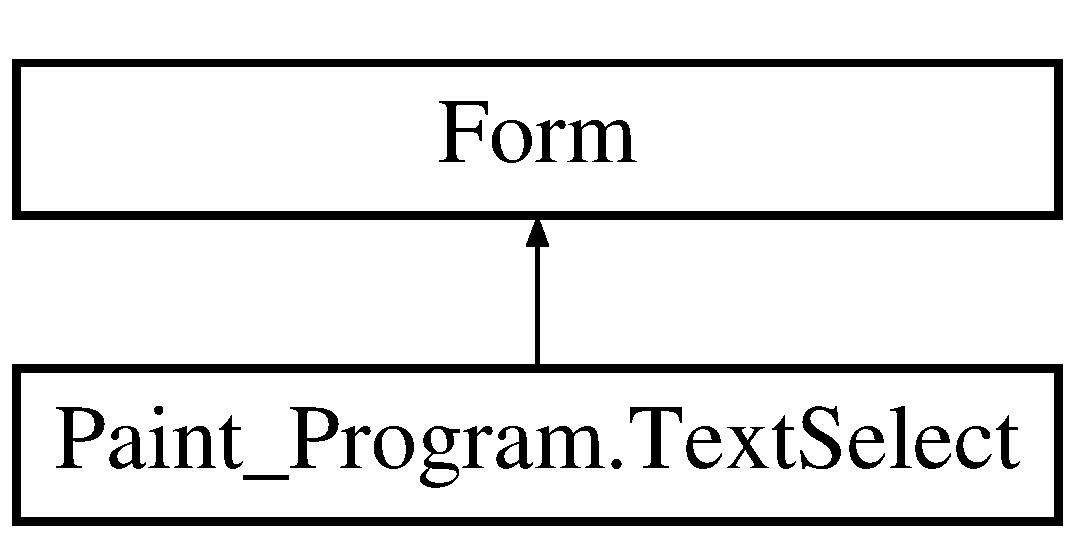
\includegraphics[height=2.000000cm]{class_paint___program_1_1_text_select}
\end{center}
\end{figure}
\subsection*{Public Member Functions}
\begin{DoxyCompactItemize}
\item 
\mbox{\hyperlink{class_paint___program_1_1_text_select_a201ea8e6ffa368c5307ae7d0ece458c8}{Text\+Select}} ()
\end{DoxyCompactItemize}
\subsection*{Protected Member Functions}
\begin{DoxyCompactItemize}
\item 
override void \mbox{\hyperlink{class_paint___program_1_1_text_select_a5ab7cbf1dde8ef28988f054a39a34905}{Dispose}} (bool disposing)
\begin{DoxyCompactList}\small\item\em Clean up any resources being used. \end{DoxyCompactList}\end{DoxyCompactItemize}
\subsection*{Properties}
\begin{DoxyCompactItemize}
\item 
string \mbox{\hyperlink{class_paint___program_1_1_text_select_a8caa6b68f423e58971e97e90cf978fea}{User\+Text}}\hspace{0.3cm}{\ttfamily  \mbox{[}get, private set\mbox{]}}
\item 
int \mbox{\hyperlink{class_paint___program_1_1_text_select_a34e1946691554cde280b2a4d3d0be64d}{Font\+Size}}\hspace{0.3cm}{\ttfamily  \mbox{[}get, private set\mbox{]}}
\item 
string \mbox{\hyperlink{class_paint___program_1_1_text_select_a3dbef208517395b1483f2d6489839025}{Font\+Type}}\hspace{0.3cm}{\ttfamily  \mbox{[}get, private set\mbox{]}}
\item 
Font\+Family \mbox{[}$\,$\mbox{]} \mbox{\hyperlink{class_paint___program_1_1_text_select_a849232d1c41d945dc2fdf80ed666a7b9}{Families}}\hspace{0.3cm}{\ttfamily  \mbox{[}get\mbox{]}}
\end{DoxyCompactItemize}
\subsection*{Private Member Functions}
\begin{DoxyCompactItemize}
\item 
void \mbox{\hyperlink{class_paint___program_1_1_text_select_ad30732ccaff1ab2ece04ca32dbbd840d}{t\+Select\+\_\+\+Click}} (object sender, Event\+Args e)
\item 
void \mbox{\hyperlink{class_paint___program_1_1_text_select_abf683438d39c8898627eeab6779ede95}{Handle\+\_\+\+Key\+Press}} (object sender, Key\+Event\+Args k)
\item 
void \mbox{\hyperlink{class_paint___program_1_1_text_select_a7b5e228f1691567c0223fea53de5958c}{Initialize\+Component}} ()
\begin{DoxyCompactList}\small\item\em Required method for Designer support -\/ do not modify the contents of this method with the code editor. \end{DoxyCompactList}\end{DoxyCompactItemize}
\subsection*{Private Attributes}
\begin{DoxyCompactItemize}
\item 
System.\+Component\+Model.\+I\+Container \mbox{\hyperlink{class_paint___program_1_1_text_select_a9556871119e1c49f176bd3f166c0ee8a}{components}} = null
\begin{DoxyCompactList}\small\item\em Required designer variable. \end{DoxyCompactList}\item 
System.\+Windows.\+Forms.\+Button \mbox{\hyperlink{class_paint___program_1_1_text_select_a1699a2f7d0d90a693f56e94b04f8938c}{t\+Select}}
\item 
System.\+Windows.\+Forms.\+Text\+Box \mbox{\hyperlink{class_paint___program_1_1_text_select_a9e312c2dd6bfb8e6a6c71e261601c282}{user\+Text}}
\item 
System.\+Windows.\+Forms.\+Text\+Box \mbox{\hyperlink{class_paint___program_1_1_text_select_a1ebaf77e711e76309db950ad8860a68b}{font\+Size}}
\item 
System.\+Windows.\+Forms.\+Combo\+Box \mbox{\hyperlink{class_paint___program_1_1_text_select_a8dda856e1399742c79fa2ce6b95a9a94}{font\+Box}}
\end{DoxyCompactItemize}


\subsection{Constructor \& Destructor Documentation}
\mbox{\Hypertarget{class_paint___program_1_1_text_select_a201ea8e6ffa368c5307ae7d0ece458c8}\label{class_paint___program_1_1_text_select_a201ea8e6ffa368c5307ae7d0ece458c8}} 
\index{Paint\+\_\+\+Program\+::\+Text\+Select@{Paint\+\_\+\+Program\+::\+Text\+Select}!Text\+Select@{Text\+Select}}
\index{Text\+Select@{Text\+Select}!Paint\+\_\+\+Program\+::\+Text\+Select@{Paint\+\_\+\+Program\+::\+Text\+Select}}
\subsubsection{\texorpdfstring{Text\+Select()}{TextSelect()}}
{\footnotesize\ttfamily Paint\+\_\+\+Program.\+Text\+Select.\+Text\+Select (\begin{DoxyParamCaption}{ }\end{DoxyParamCaption})\hspace{0.3cm}{\ttfamily [inline]}}



\subsection{Member Function Documentation}
\mbox{\Hypertarget{class_paint___program_1_1_text_select_a5ab7cbf1dde8ef28988f054a39a34905}\label{class_paint___program_1_1_text_select_a5ab7cbf1dde8ef28988f054a39a34905}} 
\index{Paint\+\_\+\+Program\+::\+Text\+Select@{Paint\+\_\+\+Program\+::\+Text\+Select}!Dispose@{Dispose}}
\index{Dispose@{Dispose}!Paint\+\_\+\+Program\+::\+Text\+Select@{Paint\+\_\+\+Program\+::\+Text\+Select}}
\subsubsection{\texorpdfstring{Dispose()}{Dispose()}}
{\footnotesize\ttfamily override void Paint\+\_\+\+Program.\+Text\+Select.\+Dispose (\begin{DoxyParamCaption}\item[{bool}]{disposing }\end{DoxyParamCaption})\hspace{0.3cm}{\ttfamily [inline]}, {\ttfamily [protected]}}



Clean up any resources being used. 


\begin{DoxyParams}{Parameters}
{\em disposing} & true if managed resources should be disposed; otherwise, false.\\
\hline
\end{DoxyParams}
\mbox{\Hypertarget{class_paint___program_1_1_text_select_abf683438d39c8898627eeab6779ede95}\label{class_paint___program_1_1_text_select_abf683438d39c8898627eeab6779ede95}} 
\index{Paint\+\_\+\+Program\+::\+Text\+Select@{Paint\+\_\+\+Program\+::\+Text\+Select}!Handle\+\_\+\+Key\+Press@{Handle\+\_\+\+Key\+Press}}
\index{Handle\+\_\+\+Key\+Press@{Handle\+\_\+\+Key\+Press}!Paint\+\_\+\+Program\+::\+Text\+Select@{Paint\+\_\+\+Program\+::\+Text\+Select}}
\subsubsection{\texorpdfstring{Handle\+\_\+\+Key\+Press()}{Handle\_KeyPress()}}
{\footnotesize\ttfamily void Paint\+\_\+\+Program.\+Text\+Select.\+Handle\+\_\+\+Key\+Press (\begin{DoxyParamCaption}\item[{object}]{sender,  }\item[{Key\+Event\+Args}]{k }\end{DoxyParamCaption})\hspace{0.3cm}{\ttfamily [inline]}, {\ttfamily [private]}}

\mbox{\Hypertarget{class_paint___program_1_1_text_select_a7b5e228f1691567c0223fea53de5958c}\label{class_paint___program_1_1_text_select_a7b5e228f1691567c0223fea53de5958c}} 
\index{Paint\+\_\+\+Program\+::\+Text\+Select@{Paint\+\_\+\+Program\+::\+Text\+Select}!Initialize\+Component@{Initialize\+Component}}
\index{Initialize\+Component@{Initialize\+Component}!Paint\+\_\+\+Program\+::\+Text\+Select@{Paint\+\_\+\+Program\+::\+Text\+Select}}
\subsubsection{\texorpdfstring{Initialize\+Component()}{InitializeComponent()}}
{\footnotesize\ttfamily void Paint\+\_\+\+Program.\+Text\+Select.\+Initialize\+Component (\begin{DoxyParamCaption}{ }\end{DoxyParamCaption})\hspace{0.3cm}{\ttfamily [inline]}, {\ttfamily [private]}}



Required method for Designer support -\/ do not modify the contents of this method with the code editor. 

\mbox{\Hypertarget{class_paint___program_1_1_text_select_ad30732ccaff1ab2ece04ca32dbbd840d}\label{class_paint___program_1_1_text_select_ad30732ccaff1ab2ece04ca32dbbd840d}} 
\index{Paint\+\_\+\+Program\+::\+Text\+Select@{Paint\+\_\+\+Program\+::\+Text\+Select}!t\+Select\+\_\+\+Click@{t\+Select\+\_\+\+Click}}
\index{t\+Select\+\_\+\+Click@{t\+Select\+\_\+\+Click}!Paint\+\_\+\+Program\+::\+Text\+Select@{Paint\+\_\+\+Program\+::\+Text\+Select}}
\subsubsection{\texorpdfstring{t\+Select\+\_\+\+Click()}{tSelect\_Click()}}
{\footnotesize\ttfamily void Paint\+\_\+\+Program.\+Text\+Select.\+t\+Select\+\_\+\+Click (\begin{DoxyParamCaption}\item[{object}]{sender,  }\item[{Event\+Args}]{e }\end{DoxyParamCaption})\hspace{0.3cm}{\ttfamily [inline]}, {\ttfamily [private]}}



\subsection{Member Data Documentation}
\mbox{\Hypertarget{class_paint___program_1_1_text_select_a9556871119e1c49f176bd3f166c0ee8a}\label{class_paint___program_1_1_text_select_a9556871119e1c49f176bd3f166c0ee8a}} 
\index{Paint\+\_\+\+Program\+::\+Text\+Select@{Paint\+\_\+\+Program\+::\+Text\+Select}!components@{components}}
\index{components@{components}!Paint\+\_\+\+Program\+::\+Text\+Select@{Paint\+\_\+\+Program\+::\+Text\+Select}}
\subsubsection{\texorpdfstring{components}{components}}
{\footnotesize\ttfamily System.\+Component\+Model.\+I\+Container Paint\+\_\+\+Program.\+Text\+Select.\+components = null\hspace{0.3cm}{\ttfamily [private]}}



Required designer variable. 

\mbox{\Hypertarget{class_paint___program_1_1_text_select_a8dda856e1399742c79fa2ce6b95a9a94}\label{class_paint___program_1_1_text_select_a8dda856e1399742c79fa2ce6b95a9a94}} 
\index{Paint\+\_\+\+Program\+::\+Text\+Select@{Paint\+\_\+\+Program\+::\+Text\+Select}!font\+Box@{font\+Box}}
\index{font\+Box@{font\+Box}!Paint\+\_\+\+Program\+::\+Text\+Select@{Paint\+\_\+\+Program\+::\+Text\+Select}}
\subsubsection{\texorpdfstring{font\+Box}{fontBox}}
{\footnotesize\ttfamily System.\+Windows.\+Forms.\+Combo\+Box Paint\+\_\+\+Program.\+Text\+Select.\+font\+Box\hspace{0.3cm}{\ttfamily [private]}}

\mbox{\Hypertarget{class_paint___program_1_1_text_select_a1ebaf77e711e76309db950ad8860a68b}\label{class_paint___program_1_1_text_select_a1ebaf77e711e76309db950ad8860a68b}} 
\index{Paint\+\_\+\+Program\+::\+Text\+Select@{Paint\+\_\+\+Program\+::\+Text\+Select}!font\+Size@{font\+Size}}
\index{font\+Size@{font\+Size}!Paint\+\_\+\+Program\+::\+Text\+Select@{Paint\+\_\+\+Program\+::\+Text\+Select}}
\subsubsection{\texorpdfstring{font\+Size}{fontSize}}
{\footnotesize\ttfamily System.\+Windows.\+Forms.\+Text\+Box Paint\+\_\+\+Program.\+Text\+Select.\+font\+Size\hspace{0.3cm}{\ttfamily [private]}}

\mbox{\Hypertarget{class_paint___program_1_1_text_select_a1699a2f7d0d90a693f56e94b04f8938c}\label{class_paint___program_1_1_text_select_a1699a2f7d0d90a693f56e94b04f8938c}} 
\index{Paint\+\_\+\+Program\+::\+Text\+Select@{Paint\+\_\+\+Program\+::\+Text\+Select}!t\+Select@{t\+Select}}
\index{t\+Select@{t\+Select}!Paint\+\_\+\+Program\+::\+Text\+Select@{Paint\+\_\+\+Program\+::\+Text\+Select}}
\subsubsection{\texorpdfstring{t\+Select}{tSelect}}
{\footnotesize\ttfamily System.\+Windows.\+Forms.\+Button Paint\+\_\+\+Program.\+Text\+Select.\+t\+Select\hspace{0.3cm}{\ttfamily [private]}}

\mbox{\Hypertarget{class_paint___program_1_1_text_select_a9e312c2dd6bfb8e6a6c71e261601c282}\label{class_paint___program_1_1_text_select_a9e312c2dd6bfb8e6a6c71e261601c282}} 
\index{Paint\+\_\+\+Program\+::\+Text\+Select@{Paint\+\_\+\+Program\+::\+Text\+Select}!user\+Text@{user\+Text}}
\index{user\+Text@{user\+Text}!Paint\+\_\+\+Program\+::\+Text\+Select@{Paint\+\_\+\+Program\+::\+Text\+Select}}
\subsubsection{\texorpdfstring{user\+Text}{userText}}
{\footnotesize\ttfamily System.\+Windows.\+Forms.\+Text\+Box Paint\+\_\+\+Program.\+Text\+Select.\+user\+Text\hspace{0.3cm}{\ttfamily [private]}}



\subsection{Property Documentation}
\mbox{\Hypertarget{class_paint___program_1_1_text_select_a849232d1c41d945dc2fdf80ed666a7b9}\label{class_paint___program_1_1_text_select_a849232d1c41d945dc2fdf80ed666a7b9}} 
\index{Paint\+\_\+\+Program\+::\+Text\+Select@{Paint\+\_\+\+Program\+::\+Text\+Select}!Families@{Families}}
\index{Families@{Families}!Paint\+\_\+\+Program\+::\+Text\+Select@{Paint\+\_\+\+Program\+::\+Text\+Select}}
\subsubsection{\texorpdfstring{Families}{Families}}
{\footnotesize\ttfamily Font\+Family \mbox{[}$\,$\mbox{]} Paint\+\_\+\+Program.\+Text\+Select.\+Families\hspace{0.3cm}{\ttfamily [get]}}

\mbox{\Hypertarget{class_paint___program_1_1_text_select_a34e1946691554cde280b2a4d3d0be64d}\label{class_paint___program_1_1_text_select_a34e1946691554cde280b2a4d3d0be64d}} 
\index{Paint\+\_\+\+Program\+::\+Text\+Select@{Paint\+\_\+\+Program\+::\+Text\+Select}!Font\+Size@{Font\+Size}}
\index{Font\+Size@{Font\+Size}!Paint\+\_\+\+Program\+::\+Text\+Select@{Paint\+\_\+\+Program\+::\+Text\+Select}}
\subsubsection{\texorpdfstring{Font\+Size}{FontSize}}
{\footnotesize\ttfamily int Paint\+\_\+\+Program.\+Text\+Select.\+Font\+Size\hspace{0.3cm}{\ttfamily [get]}, {\ttfamily [private set]}}

\mbox{\Hypertarget{class_paint___program_1_1_text_select_a3dbef208517395b1483f2d6489839025}\label{class_paint___program_1_1_text_select_a3dbef208517395b1483f2d6489839025}} 
\index{Paint\+\_\+\+Program\+::\+Text\+Select@{Paint\+\_\+\+Program\+::\+Text\+Select}!Font\+Type@{Font\+Type}}
\index{Font\+Type@{Font\+Type}!Paint\+\_\+\+Program\+::\+Text\+Select@{Paint\+\_\+\+Program\+::\+Text\+Select}}
\subsubsection{\texorpdfstring{Font\+Type}{FontType}}
{\footnotesize\ttfamily string Paint\+\_\+\+Program.\+Text\+Select.\+Font\+Type\hspace{0.3cm}{\ttfamily [get]}, {\ttfamily [private set]}}

\mbox{\Hypertarget{class_paint___program_1_1_text_select_a8caa6b68f423e58971e97e90cf978fea}\label{class_paint___program_1_1_text_select_a8caa6b68f423e58971e97e90cf978fea}} 
\index{Paint\+\_\+\+Program\+::\+Text\+Select@{Paint\+\_\+\+Program\+::\+Text\+Select}!User\+Text@{User\+Text}}
\index{User\+Text@{User\+Text}!Paint\+\_\+\+Program\+::\+Text\+Select@{Paint\+\_\+\+Program\+::\+Text\+Select}}
\subsubsection{\texorpdfstring{User\+Text}{UserText}}
{\footnotesize\ttfamily string Paint\+\_\+\+Program.\+Text\+Select.\+User\+Text\hspace{0.3cm}{\ttfamily [get]}, {\ttfamily [private set]}}



The documentation for this class was generated from the following files\+:\begin{DoxyCompactItemize}
\item 
Paint Program/\mbox{\hyperlink{_text_select_8cs}{Text\+Select.\+cs}}\item 
Paint Program/\mbox{\hyperlink{_text_select_8_designer_8cs}{Text\+Select.\+Designer.\+cs}}\end{DoxyCompactItemize}

\hypertarget{class_paint___program_1_1_text_tool}{}\section{Paint\+\_\+\+Program.\+Text\+Tool Class Reference}
\label{class_paint___program_1_1_text_tool}\index{Paint\+\_\+\+Program.\+Text\+Tool@{Paint\+\_\+\+Program.\+Text\+Tool}}
Inheritance diagram for Paint\+\_\+\+Program.\+Text\+Tool\+:\begin{figure}[H]
\begin{center}
\leavevmode
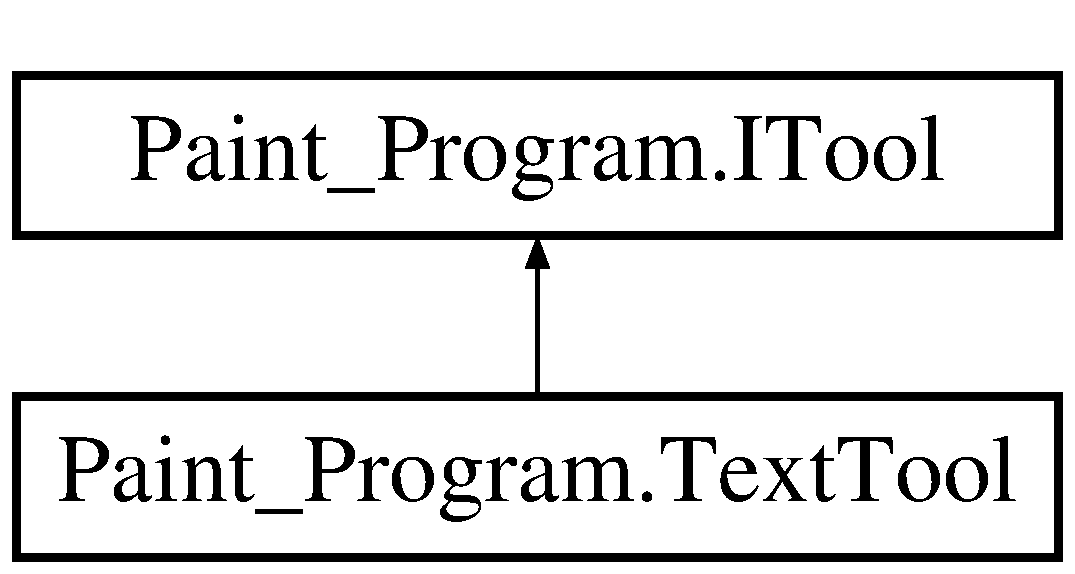
\includegraphics[height=2.000000cm]{class_paint___program_1_1_text_tool}
\end{center}
\end{figure}
\subsection*{Public Member Functions}
\begin{DoxyCompactItemize}
\item 
\mbox{\hyperlink{class_paint___program_1_1_text_tool_a600ec6a0003ca544a857f7e6a79f5688}{Text\+Tool}} ()
\item 
void \mbox{\hyperlink{class_paint___program_1_1_text_tool_a8351e31f6387ff80cbff288a73a10a3d}{Init}} ()
\item 
string \mbox{\hyperlink{class_paint___program_1_1_text_tool_a0adfe4c942f7d97c2d9cf626fb3b78c7}{Get\+Tool\+Icon\+Path}} ()
\item 
bool \mbox{\hyperlink{class_paint___program_1_1_text_tool_a053b13ff961f302f816b57ab5c48952a}{is\+Initalized}} ()
\item 
void \mbox{\hyperlink{class_paint___program_1_1_text_tool_a56294ea8e94d8aa58282660c24eb74bb}{On\+Mouse\+Down}} (object sender, Mouse\+Event\+Args e)
\item 
void \mbox{\hyperlink{class_paint___program_1_1_text_tool_a25bd60db2eeff1a131bce076e7f68757}{On\+Mouse\+Move}} (object sender, Mouse\+Event\+Args e)
\item 
void \mbox{\hyperlink{class_paint___program_1_1_text_tool_a0b77db4478e19cd1f957c37af981fbf5}{On\+Mouse\+Up}} (object sender, Mouse\+Event\+Args e)
\item 
Bitmap \mbox{\hyperlink{class_paint___program_1_1_text_tool_acb2114b449f982664f1fd49e3bb0b017}{Get\+Tool\+Layer}} ()
\item 
bool \mbox{\hyperlink{class_paint___program_1_1_text_tool_a6fdb8fac7060beb3677489c709a7913f}{Requires\+Layer\+Data}} ()
\item 
void \mbox{\hyperlink{class_paint___program_1_1_text_tool_a3022ee066b3c9dfdff596027c3a184ed}{Set\+Layer\+Data}} (Bitmap bit)
\item 
string \mbox{\hyperlink{class_paint___program_1_1_text_tool_a39c92c312fa71a01a3ce97c2c0293c25}{Get\+Tool\+Tip}} ()
\item 
void \mbox{\hyperlink{class_paint___program_1_1_text_tool_a7fdf6ff8d7fa9bf43cbb4c6668862f2c}{Update\+Interface\+Layer}} ()
\end{DoxyCompactItemize}
\subsection*{Private Attributes}
\begin{DoxyCompactItemize}
\item 
Graphics \mbox{\hyperlink{class_paint___program_1_1_text_tool_aebcdbc77df8cc28b59213744989d2b74}{graphics}}
\item 
int \mbox{\hyperlink{class_paint___program_1_1_text_tool_a77267cf0c8405057fb527c0ac3e81229}{width}}
\item 
int \mbox{\hyperlink{class_paint___program_1_1_text_tool_ab6ddb1da76c16dd70e8d1682d0770b41}{height}}
\item 
bool \mbox{\hyperlink{class_paint___program_1_1_text_tool_a2f0edf40e994616034bd0c71ce1d1735}{b\+Active}}
\item 
bool \mbox{\hyperlink{class_paint___program_1_1_text_tool_a9a3ba132a7bc742c7dede40be6bbeeee}{b\+Mouse\+Down}}
\item 
bool \mbox{\hyperlink{class_paint___program_1_1_text_tool_a7e8cc3ec53e73fc57bc1f6c698654bb1}{b\+Init}}
\item 
Point \mbox{\hyperlink{class_paint___program_1_1_text_tool_ad0b053bdd29fa0a048dd743305ad76b3}{p\+Old}}
\item 
Point \mbox{\hyperlink{class_paint___program_1_1_text_tool_ad3f0da3f42463a6c21694898bfb37f7d}{p\+New}}
\item 
SizeF \mbox{\hyperlink{class_paint___program_1_1_text_tool_a2fe7070d05a4b5970daf782a2cd3a54b}{t\+Size}}
\item 
Color \mbox{\hyperlink{class_paint___program_1_1_text_tool_af0636766c9cdf1139840aaa79a513cd9}{font\+Color}}
\end{DoxyCompactItemize}


\subsection{Constructor \& Destructor Documentation}
\mbox{\Hypertarget{class_paint___program_1_1_text_tool_a600ec6a0003ca544a857f7e6a79f5688}\label{class_paint___program_1_1_text_tool_a600ec6a0003ca544a857f7e6a79f5688}} 
\index{Paint\+\_\+\+Program\+::\+Text\+Tool@{Paint\+\_\+\+Program\+::\+Text\+Tool}!Text\+Tool@{Text\+Tool}}
\index{Text\+Tool@{Text\+Tool}!Paint\+\_\+\+Program\+::\+Text\+Tool@{Paint\+\_\+\+Program\+::\+Text\+Tool}}
\subsubsection{\texorpdfstring{Text\+Tool()}{TextTool()}}
{\footnotesize\ttfamily Paint\+\_\+\+Program.\+Text\+Tool.\+Text\+Tool (\begin{DoxyParamCaption}{ }\end{DoxyParamCaption})\hspace{0.3cm}{\ttfamily [inline]}}



\subsection{Member Function Documentation}
\mbox{\Hypertarget{class_paint___program_1_1_text_tool_a0adfe4c942f7d97c2d9cf626fb3b78c7}\label{class_paint___program_1_1_text_tool_a0adfe4c942f7d97c2d9cf626fb3b78c7}} 
\index{Paint\+\_\+\+Program\+::\+Text\+Tool@{Paint\+\_\+\+Program\+::\+Text\+Tool}!Get\+Tool\+Icon\+Path@{Get\+Tool\+Icon\+Path}}
\index{Get\+Tool\+Icon\+Path@{Get\+Tool\+Icon\+Path}!Paint\+\_\+\+Program\+::\+Text\+Tool@{Paint\+\_\+\+Program\+::\+Text\+Tool}}
\subsubsection{\texorpdfstring{Get\+Tool\+Icon\+Path()}{GetToolIconPath()}}
{\footnotesize\ttfamily string Paint\+\_\+\+Program.\+Text\+Tool.\+Get\+Tool\+Icon\+Path (\begin{DoxyParamCaption}{ }\end{DoxyParamCaption})\hspace{0.3cm}{\ttfamily [inline]}}



Implements \mbox{\hyperlink{interface_paint___program_1_1_i_tool_aa057d2f99c59d7bec0215dcad2da1b72}{Paint\+\_\+\+Program.\+I\+Tool}}.

\mbox{\Hypertarget{class_paint___program_1_1_text_tool_acb2114b449f982664f1fd49e3bb0b017}\label{class_paint___program_1_1_text_tool_acb2114b449f982664f1fd49e3bb0b017}} 
\index{Paint\+\_\+\+Program\+::\+Text\+Tool@{Paint\+\_\+\+Program\+::\+Text\+Tool}!Get\+Tool\+Layer@{Get\+Tool\+Layer}}
\index{Get\+Tool\+Layer@{Get\+Tool\+Layer}!Paint\+\_\+\+Program\+::\+Text\+Tool@{Paint\+\_\+\+Program\+::\+Text\+Tool}}
\subsubsection{\texorpdfstring{Get\+Tool\+Layer()}{GetToolLayer()}}
{\footnotesize\ttfamily Bitmap Paint\+\_\+\+Program.\+Text\+Tool.\+Get\+Tool\+Layer (\begin{DoxyParamCaption}{ }\end{DoxyParamCaption})\hspace{0.3cm}{\ttfamily [inline]}}



Implements \mbox{\hyperlink{interface_paint___program_1_1_i_tool_a9b057905515f42a988c166a6a40318e0}{Paint\+\_\+\+Program.\+I\+Tool}}.

\mbox{\Hypertarget{class_paint___program_1_1_text_tool_a39c92c312fa71a01a3ce97c2c0293c25}\label{class_paint___program_1_1_text_tool_a39c92c312fa71a01a3ce97c2c0293c25}} 
\index{Paint\+\_\+\+Program\+::\+Text\+Tool@{Paint\+\_\+\+Program\+::\+Text\+Tool}!Get\+Tool\+Tip@{Get\+Tool\+Tip}}
\index{Get\+Tool\+Tip@{Get\+Tool\+Tip}!Paint\+\_\+\+Program\+::\+Text\+Tool@{Paint\+\_\+\+Program\+::\+Text\+Tool}}
\subsubsection{\texorpdfstring{Get\+Tool\+Tip()}{GetToolTip()}}
{\footnotesize\ttfamily string Paint\+\_\+\+Program.\+Text\+Tool.\+Get\+Tool\+Tip (\begin{DoxyParamCaption}{ }\end{DoxyParamCaption})\hspace{0.3cm}{\ttfamily [inline]}}



Implements \mbox{\hyperlink{interface_paint___program_1_1_i_tool_ac11f1591587144b6e74f5767bbf1df56}{Paint\+\_\+\+Program.\+I\+Tool}}.

\mbox{\Hypertarget{class_paint___program_1_1_text_tool_a8351e31f6387ff80cbff288a73a10a3d}\label{class_paint___program_1_1_text_tool_a8351e31f6387ff80cbff288a73a10a3d}} 
\index{Paint\+\_\+\+Program\+::\+Text\+Tool@{Paint\+\_\+\+Program\+::\+Text\+Tool}!Init@{Init}}
\index{Init@{Init}!Paint\+\_\+\+Program\+::\+Text\+Tool@{Paint\+\_\+\+Program\+::\+Text\+Tool}}
\subsubsection{\texorpdfstring{Init()}{Init()}}
{\footnotesize\ttfamily void Paint\+\_\+\+Program.\+Text\+Tool.\+Init (\begin{DoxyParamCaption}{ }\end{DoxyParamCaption})\hspace{0.3cm}{\ttfamily [inline]}}



Implements \mbox{\hyperlink{interface_paint___program_1_1_i_tool_af823123a30fbda34e24e907243241046}{Paint\+\_\+\+Program.\+I\+Tool}}.

\mbox{\Hypertarget{class_paint___program_1_1_text_tool_a053b13ff961f302f816b57ab5c48952a}\label{class_paint___program_1_1_text_tool_a053b13ff961f302f816b57ab5c48952a}} 
\index{Paint\+\_\+\+Program\+::\+Text\+Tool@{Paint\+\_\+\+Program\+::\+Text\+Tool}!is\+Initalized@{is\+Initalized}}
\index{is\+Initalized@{is\+Initalized}!Paint\+\_\+\+Program\+::\+Text\+Tool@{Paint\+\_\+\+Program\+::\+Text\+Tool}}
\subsubsection{\texorpdfstring{is\+Initalized()}{isInitalized()}}
{\footnotesize\ttfamily bool Paint\+\_\+\+Program.\+Text\+Tool.\+is\+Initalized (\begin{DoxyParamCaption}{ }\end{DoxyParamCaption})\hspace{0.3cm}{\ttfamily [inline]}}



Implements \mbox{\hyperlink{interface_paint___program_1_1_i_tool_a951b844bcbf47a6c306104fa86be7a5d}{Paint\+\_\+\+Program.\+I\+Tool}}.

\mbox{\Hypertarget{class_paint___program_1_1_text_tool_a56294ea8e94d8aa58282660c24eb74bb}\label{class_paint___program_1_1_text_tool_a56294ea8e94d8aa58282660c24eb74bb}} 
\index{Paint\+\_\+\+Program\+::\+Text\+Tool@{Paint\+\_\+\+Program\+::\+Text\+Tool}!On\+Mouse\+Down@{On\+Mouse\+Down}}
\index{On\+Mouse\+Down@{On\+Mouse\+Down}!Paint\+\_\+\+Program\+::\+Text\+Tool@{Paint\+\_\+\+Program\+::\+Text\+Tool}}
\subsubsection{\texorpdfstring{On\+Mouse\+Down()}{OnMouseDown()}}
{\footnotesize\ttfamily void Paint\+\_\+\+Program.\+Text\+Tool.\+On\+Mouse\+Down (\begin{DoxyParamCaption}\item[{object}]{sender,  }\item[{Mouse\+Event\+Args}]{e }\end{DoxyParamCaption})\hspace{0.3cm}{\ttfamily [inline]}}



Implements \mbox{\hyperlink{interface_paint___program_1_1_i_tool_a73d8797f4f2b1e0d8efe8aadcd44e840}{Paint\+\_\+\+Program.\+I\+Tool}}.

\mbox{\Hypertarget{class_paint___program_1_1_text_tool_a25bd60db2eeff1a131bce076e7f68757}\label{class_paint___program_1_1_text_tool_a25bd60db2eeff1a131bce076e7f68757}} 
\index{Paint\+\_\+\+Program\+::\+Text\+Tool@{Paint\+\_\+\+Program\+::\+Text\+Tool}!On\+Mouse\+Move@{On\+Mouse\+Move}}
\index{On\+Mouse\+Move@{On\+Mouse\+Move}!Paint\+\_\+\+Program\+::\+Text\+Tool@{Paint\+\_\+\+Program\+::\+Text\+Tool}}
\subsubsection{\texorpdfstring{On\+Mouse\+Move()}{OnMouseMove()}}
{\footnotesize\ttfamily void Paint\+\_\+\+Program.\+Text\+Tool.\+On\+Mouse\+Move (\begin{DoxyParamCaption}\item[{object}]{sender,  }\item[{Mouse\+Event\+Args}]{e }\end{DoxyParamCaption})\hspace{0.3cm}{\ttfamily [inline]}}



Implements \mbox{\hyperlink{interface_paint___program_1_1_i_tool_a6a1cbe840b5cfc8a9b9463cc21590845}{Paint\+\_\+\+Program.\+I\+Tool}}.

\mbox{\Hypertarget{class_paint___program_1_1_text_tool_a0b77db4478e19cd1f957c37af981fbf5}\label{class_paint___program_1_1_text_tool_a0b77db4478e19cd1f957c37af981fbf5}} 
\index{Paint\+\_\+\+Program\+::\+Text\+Tool@{Paint\+\_\+\+Program\+::\+Text\+Tool}!On\+Mouse\+Up@{On\+Mouse\+Up}}
\index{On\+Mouse\+Up@{On\+Mouse\+Up}!Paint\+\_\+\+Program\+::\+Text\+Tool@{Paint\+\_\+\+Program\+::\+Text\+Tool}}
\subsubsection{\texorpdfstring{On\+Mouse\+Up()}{OnMouseUp()}}
{\footnotesize\ttfamily void Paint\+\_\+\+Program.\+Text\+Tool.\+On\+Mouse\+Up (\begin{DoxyParamCaption}\item[{object}]{sender,  }\item[{Mouse\+Event\+Args}]{e }\end{DoxyParamCaption})\hspace{0.3cm}{\ttfamily [inline]}}



Implements \mbox{\hyperlink{interface_paint___program_1_1_i_tool_a47984c2879213022f1684c07f7bba73e}{Paint\+\_\+\+Program.\+I\+Tool}}.

\mbox{\Hypertarget{class_paint___program_1_1_text_tool_a6fdb8fac7060beb3677489c709a7913f}\label{class_paint___program_1_1_text_tool_a6fdb8fac7060beb3677489c709a7913f}} 
\index{Paint\+\_\+\+Program\+::\+Text\+Tool@{Paint\+\_\+\+Program\+::\+Text\+Tool}!Requires\+Layer\+Data@{Requires\+Layer\+Data}}
\index{Requires\+Layer\+Data@{Requires\+Layer\+Data}!Paint\+\_\+\+Program\+::\+Text\+Tool@{Paint\+\_\+\+Program\+::\+Text\+Tool}}
\subsubsection{\texorpdfstring{Requires\+Layer\+Data()}{RequiresLayerData()}}
{\footnotesize\ttfamily bool Paint\+\_\+\+Program.\+Text\+Tool.\+Requires\+Layer\+Data (\begin{DoxyParamCaption}{ }\end{DoxyParamCaption})\hspace{0.3cm}{\ttfamily [inline]}}



Implements \mbox{\hyperlink{interface_paint___program_1_1_i_tool_a6d45b6c48da8130ae41db3a66cdaef9a}{Paint\+\_\+\+Program.\+I\+Tool}}.

\mbox{\Hypertarget{class_paint___program_1_1_text_tool_a3022ee066b3c9dfdff596027c3a184ed}\label{class_paint___program_1_1_text_tool_a3022ee066b3c9dfdff596027c3a184ed}} 
\index{Paint\+\_\+\+Program\+::\+Text\+Tool@{Paint\+\_\+\+Program\+::\+Text\+Tool}!Set\+Layer\+Data@{Set\+Layer\+Data}}
\index{Set\+Layer\+Data@{Set\+Layer\+Data}!Paint\+\_\+\+Program\+::\+Text\+Tool@{Paint\+\_\+\+Program\+::\+Text\+Tool}}
\subsubsection{\texorpdfstring{Set\+Layer\+Data()}{SetLayerData()}}
{\footnotesize\ttfamily void Paint\+\_\+\+Program.\+Text\+Tool.\+Set\+Layer\+Data (\begin{DoxyParamCaption}\item[{Bitmap}]{bit }\end{DoxyParamCaption})\hspace{0.3cm}{\ttfamily [inline]}}



Implements \mbox{\hyperlink{interface_paint___program_1_1_i_tool_a2d3e63715dfe04075d27dacf367d1633}{Paint\+\_\+\+Program.\+I\+Tool}}.

\mbox{\Hypertarget{class_paint___program_1_1_text_tool_a7fdf6ff8d7fa9bf43cbb4c6668862f2c}\label{class_paint___program_1_1_text_tool_a7fdf6ff8d7fa9bf43cbb4c6668862f2c}} 
\index{Paint\+\_\+\+Program\+::\+Text\+Tool@{Paint\+\_\+\+Program\+::\+Text\+Tool}!Update\+Interface\+Layer@{Update\+Interface\+Layer}}
\index{Update\+Interface\+Layer@{Update\+Interface\+Layer}!Paint\+\_\+\+Program\+::\+Text\+Tool@{Paint\+\_\+\+Program\+::\+Text\+Tool}}
\subsubsection{\texorpdfstring{Update\+Interface\+Layer()}{UpdateInterfaceLayer()}}
{\footnotesize\ttfamily void Paint\+\_\+\+Program.\+Text\+Tool.\+Update\+Interface\+Layer (\begin{DoxyParamCaption}{ }\end{DoxyParamCaption})\hspace{0.3cm}{\ttfamily [inline]}}



Implements \mbox{\hyperlink{interface_paint___program_1_1_i_tool_a36db75d29e88dfd739f658633c40e955}{Paint\+\_\+\+Program.\+I\+Tool}}.



\subsection{Member Data Documentation}
\mbox{\Hypertarget{class_paint___program_1_1_text_tool_a2f0edf40e994616034bd0c71ce1d1735}\label{class_paint___program_1_1_text_tool_a2f0edf40e994616034bd0c71ce1d1735}} 
\index{Paint\+\_\+\+Program\+::\+Text\+Tool@{Paint\+\_\+\+Program\+::\+Text\+Tool}!b\+Active@{b\+Active}}
\index{b\+Active@{b\+Active}!Paint\+\_\+\+Program\+::\+Text\+Tool@{Paint\+\_\+\+Program\+::\+Text\+Tool}}
\subsubsection{\texorpdfstring{b\+Active}{bActive}}
{\footnotesize\ttfamily bool Paint\+\_\+\+Program.\+Text\+Tool.\+b\+Active\hspace{0.3cm}{\ttfamily [private]}}

\mbox{\Hypertarget{class_paint___program_1_1_text_tool_a7e8cc3ec53e73fc57bc1f6c698654bb1}\label{class_paint___program_1_1_text_tool_a7e8cc3ec53e73fc57bc1f6c698654bb1}} 
\index{Paint\+\_\+\+Program\+::\+Text\+Tool@{Paint\+\_\+\+Program\+::\+Text\+Tool}!b\+Init@{b\+Init}}
\index{b\+Init@{b\+Init}!Paint\+\_\+\+Program\+::\+Text\+Tool@{Paint\+\_\+\+Program\+::\+Text\+Tool}}
\subsubsection{\texorpdfstring{b\+Init}{bInit}}
{\footnotesize\ttfamily bool Paint\+\_\+\+Program.\+Text\+Tool.\+b\+Init\hspace{0.3cm}{\ttfamily [private]}}

\mbox{\Hypertarget{class_paint___program_1_1_text_tool_a9a3ba132a7bc742c7dede40be6bbeeee}\label{class_paint___program_1_1_text_tool_a9a3ba132a7bc742c7dede40be6bbeeee}} 
\index{Paint\+\_\+\+Program\+::\+Text\+Tool@{Paint\+\_\+\+Program\+::\+Text\+Tool}!b\+Mouse\+Down@{b\+Mouse\+Down}}
\index{b\+Mouse\+Down@{b\+Mouse\+Down}!Paint\+\_\+\+Program\+::\+Text\+Tool@{Paint\+\_\+\+Program\+::\+Text\+Tool}}
\subsubsection{\texorpdfstring{b\+Mouse\+Down}{bMouseDown}}
{\footnotesize\ttfamily bool Paint\+\_\+\+Program.\+Text\+Tool.\+b\+Mouse\+Down\hspace{0.3cm}{\ttfamily [private]}}

\mbox{\Hypertarget{class_paint___program_1_1_text_tool_af0636766c9cdf1139840aaa79a513cd9}\label{class_paint___program_1_1_text_tool_af0636766c9cdf1139840aaa79a513cd9}} 
\index{Paint\+\_\+\+Program\+::\+Text\+Tool@{Paint\+\_\+\+Program\+::\+Text\+Tool}!font\+Color@{font\+Color}}
\index{font\+Color@{font\+Color}!Paint\+\_\+\+Program\+::\+Text\+Tool@{Paint\+\_\+\+Program\+::\+Text\+Tool}}
\subsubsection{\texorpdfstring{font\+Color}{fontColor}}
{\footnotesize\ttfamily Color Paint\+\_\+\+Program.\+Text\+Tool.\+font\+Color\hspace{0.3cm}{\ttfamily [private]}}

\mbox{\Hypertarget{class_paint___program_1_1_text_tool_aebcdbc77df8cc28b59213744989d2b74}\label{class_paint___program_1_1_text_tool_aebcdbc77df8cc28b59213744989d2b74}} 
\index{Paint\+\_\+\+Program\+::\+Text\+Tool@{Paint\+\_\+\+Program\+::\+Text\+Tool}!graphics@{graphics}}
\index{graphics@{graphics}!Paint\+\_\+\+Program\+::\+Text\+Tool@{Paint\+\_\+\+Program\+::\+Text\+Tool}}
\subsubsection{\texorpdfstring{graphics}{graphics}}
{\footnotesize\ttfamily Graphics Paint\+\_\+\+Program.\+Text\+Tool.\+graphics\hspace{0.3cm}{\ttfamily [private]}}

\mbox{\Hypertarget{class_paint___program_1_1_text_tool_ab6ddb1da76c16dd70e8d1682d0770b41}\label{class_paint___program_1_1_text_tool_ab6ddb1da76c16dd70e8d1682d0770b41}} 
\index{Paint\+\_\+\+Program\+::\+Text\+Tool@{Paint\+\_\+\+Program\+::\+Text\+Tool}!height@{height}}
\index{height@{height}!Paint\+\_\+\+Program\+::\+Text\+Tool@{Paint\+\_\+\+Program\+::\+Text\+Tool}}
\subsubsection{\texorpdfstring{height}{height}}
{\footnotesize\ttfamily int Paint\+\_\+\+Program.\+Text\+Tool.\+height\hspace{0.3cm}{\ttfamily [private]}}

\mbox{\Hypertarget{class_paint___program_1_1_text_tool_ad3f0da3f42463a6c21694898bfb37f7d}\label{class_paint___program_1_1_text_tool_ad3f0da3f42463a6c21694898bfb37f7d}} 
\index{Paint\+\_\+\+Program\+::\+Text\+Tool@{Paint\+\_\+\+Program\+::\+Text\+Tool}!p\+New@{p\+New}}
\index{p\+New@{p\+New}!Paint\+\_\+\+Program\+::\+Text\+Tool@{Paint\+\_\+\+Program\+::\+Text\+Tool}}
\subsubsection{\texorpdfstring{p\+New}{pNew}}
{\footnotesize\ttfamily Point Paint\+\_\+\+Program.\+Text\+Tool.\+p\+New\hspace{0.3cm}{\ttfamily [private]}}

\mbox{\Hypertarget{class_paint___program_1_1_text_tool_ad0b053bdd29fa0a048dd743305ad76b3}\label{class_paint___program_1_1_text_tool_ad0b053bdd29fa0a048dd743305ad76b3}} 
\index{Paint\+\_\+\+Program\+::\+Text\+Tool@{Paint\+\_\+\+Program\+::\+Text\+Tool}!p\+Old@{p\+Old}}
\index{p\+Old@{p\+Old}!Paint\+\_\+\+Program\+::\+Text\+Tool@{Paint\+\_\+\+Program\+::\+Text\+Tool}}
\subsubsection{\texorpdfstring{p\+Old}{pOld}}
{\footnotesize\ttfamily Point Paint\+\_\+\+Program.\+Text\+Tool.\+p\+Old\hspace{0.3cm}{\ttfamily [private]}}

\mbox{\Hypertarget{class_paint___program_1_1_text_tool_a2fe7070d05a4b5970daf782a2cd3a54b}\label{class_paint___program_1_1_text_tool_a2fe7070d05a4b5970daf782a2cd3a54b}} 
\index{Paint\+\_\+\+Program\+::\+Text\+Tool@{Paint\+\_\+\+Program\+::\+Text\+Tool}!t\+Size@{t\+Size}}
\index{t\+Size@{t\+Size}!Paint\+\_\+\+Program\+::\+Text\+Tool@{Paint\+\_\+\+Program\+::\+Text\+Tool}}
\subsubsection{\texorpdfstring{t\+Size}{tSize}}
{\footnotesize\ttfamily SizeF Paint\+\_\+\+Program.\+Text\+Tool.\+t\+Size\hspace{0.3cm}{\ttfamily [private]}}

\mbox{\Hypertarget{class_paint___program_1_1_text_tool_a77267cf0c8405057fb527c0ac3e81229}\label{class_paint___program_1_1_text_tool_a77267cf0c8405057fb527c0ac3e81229}} 
\index{Paint\+\_\+\+Program\+::\+Text\+Tool@{Paint\+\_\+\+Program\+::\+Text\+Tool}!width@{width}}
\index{width@{width}!Paint\+\_\+\+Program\+::\+Text\+Tool@{Paint\+\_\+\+Program\+::\+Text\+Tool}}
\subsubsection{\texorpdfstring{width}{width}}
{\footnotesize\ttfamily int Paint\+\_\+\+Program.\+Text\+Tool.\+width\hspace{0.3cm}{\ttfamily [private]}}



The documentation for this class was generated from the following file\+:\begin{DoxyCompactItemize}
\item 
Paint Program/\mbox{\hyperlink{_text_tool_8cs}{Text\+Tool.\+cs}}\end{DoxyCompactItemize}

\hypertarget{struct_wintab_d_n_1_1_wintab_axis}{}\section{Wintab\+D\+N.\+Wintab\+Axis Struct Reference}
\label{struct_wintab_d_n_1_1_wintab_axis}\index{Wintab\+D\+N.\+Wintab\+Axis@{Wintab\+D\+N.\+Wintab\+Axis}}


Managed version of A\+X\+IS struct.  


\subsection*{Public Attributes}
\begin{DoxyCompactItemize}
\item 
Int32 \mbox{\hyperlink{struct_wintab_d_n_1_1_wintab_axis_a66135b352cd339fba0a8ab157d454d22}{ax\+Min}}
\begin{DoxyCompactList}\small\item\em Specifies the minimum value of the data item in the tablet\textquotesingle{}s na-\/tive coordinates. \end{DoxyCompactList}\item 
Int32 \mbox{\hyperlink{struct_wintab_d_n_1_1_wintab_axis_ad808a5058b80cd5b14e8dca275550cf7}{ax\+Max}}
\begin{DoxyCompactList}\small\item\em Specifies the maximum value of the data item in the tablet\textquotesingle{}s na-\/tive coordinates. \end{DoxyCompactList}\item 
U\+Int32 \mbox{\hyperlink{struct_wintab_d_n_1_1_wintab_axis_a571eed7c1e0ceb7cb44b1da7b2eaca69}{ax\+Units}}
\begin{DoxyCompactList}\small\item\em Indicates the units used in calculating the resolution for the data item. \end{DoxyCompactList}\item 
\mbox{\hyperlink{class_wintab_d_n_1_1_f_i_x32}{F\+I\+X32}} \mbox{\hyperlink{struct_wintab_d_n_1_1_wintab_axis_a811551f70bc21a049c9562eb8ab934da}{ax\+Resolution}}
\begin{DoxyCompactList}\small\item\em Is a fixed-\/point number giving the number of data item incre-\/ments per physical unit. \end{DoxyCompactList}\end{DoxyCompactItemize}


\subsection{Detailed Description}
Managed version of A\+X\+IS struct. 



\subsection{Member Data Documentation}
\mbox{\Hypertarget{struct_wintab_d_n_1_1_wintab_axis_ad808a5058b80cd5b14e8dca275550cf7}\label{struct_wintab_d_n_1_1_wintab_axis_ad808a5058b80cd5b14e8dca275550cf7}} 
\index{Wintab\+D\+N\+::\+Wintab\+Axis@{Wintab\+D\+N\+::\+Wintab\+Axis}!ax\+Max@{ax\+Max}}
\index{ax\+Max@{ax\+Max}!Wintab\+D\+N\+::\+Wintab\+Axis@{Wintab\+D\+N\+::\+Wintab\+Axis}}
\subsubsection{\texorpdfstring{ax\+Max}{axMax}}
{\footnotesize\ttfamily Int32 Wintab\+D\+N.\+Wintab\+Axis.\+ax\+Max}



Specifies the maximum value of the data item in the tablet\textquotesingle{}s na-\/tive coordinates. 

\mbox{\Hypertarget{struct_wintab_d_n_1_1_wintab_axis_a66135b352cd339fba0a8ab157d454d22}\label{struct_wintab_d_n_1_1_wintab_axis_a66135b352cd339fba0a8ab157d454d22}} 
\index{Wintab\+D\+N\+::\+Wintab\+Axis@{Wintab\+D\+N\+::\+Wintab\+Axis}!ax\+Min@{ax\+Min}}
\index{ax\+Min@{ax\+Min}!Wintab\+D\+N\+::\+Wintab\+Axis@{Wintab\+D\+N\+::\+Wintab\+Axis}}
\subsubsection{\texorpdfstring{ax\+Min}{axMin}}
{\footnotesize\ttfamily Int32 Wintab\+D\+N.\+Wintab\+Axis.\+ax\+Min}



Specifies the minimum value of the data item in the tablet\textquotesingle{}s na-\/tive coordinates. 

\mbox{\Hypertarget{struct_wintab_d_n_1_1_wintab_axis_a811551f70bc21a049c9562eb8ab934da}\label{struct_wintab_d_n_1_1_wintab_axis_a811551f70bc21a049c9562eb8ab934da}} 
\index{Wintab\+D\+N\+::\+Wintab\+Axis@{Wintab\+D\+N\+::\+Wintab\+Axis}!ax\+Resolution@{ax\+Resolution}}
\index{ax\+Resolution@{ax\+Resolution}!Wintab\+D\+N\+::\+Wintab\+Axis@{Wintab\+D\+N\+::\+Wintab\+Axis}}
\subsubsection{\texorpdfstring{ax\+Resolution}{axResolution}}
{\footnotesize\ttfamily \mbox{\hyperlink{class_wintab_d_n_1_1_f_i_x32}{F\+I\+X32}} Wintab\+D\+N.\+Wintab\+Axis.\+ax\+Resolution}



Is a fixed-\/point number giving the number of data item incre-\/ments per physical unit. 

\mbox{\Hypertarget{struct_wintab_d_n_1_1_wintab_axis_a571eed7c1e0ceb7cb44b1da7b2eaca69}\label{struct_wintab_d_n_1_1_wintab_axis_a571eed7c1e0ceb7cb44b1da7b2eaca69}} 
\index{Wintab\+D\+N\+::\+Wintab\+Axis@{Wintab\+D\+N\+::\+Wintab\+Axis}!ax\+Units@{ax\+Units}}
\index{ax\+Units@{ax\+Units}!Wintab\+D\+N\+::\+Wintab\+Axis@{Wintab\+D\+N\+::\+Wintab\+Axis}}
\subsubsection{\texorpdfstring{ax\+Units}{axUnits}}
{\footnotesize\ttfamily U\+Int32 Wintab\+D\+N.\+Wintab\+Axis.\+ax\+Units}



Indicates the units used in calculating the resolution for the data item. 



The documentation for this struct was generated from the following file\+:\begin{DoxyCompactItemize}
\item 
Wintab\+D\+N/\mbox{\hyperlink{_c_wintab_context_8cs}{C\+Wintab\+Context.\+cs}}\end{DoxyCompactItemize}

\hypertarget{struct_wintab_d_n_1_1_wintab_axis_array}{}\section{Wintab\+D\+N.\+Wintab\+Axis\+Array Struct Reference}
\label{struct_wintab_d_n_1_1_wintab_axis_array}\index{Wintab\+D\+N.\+Wintab\+Axis\+Array@{Wintab\+D\+N.\+Wintab\+Axis\+Array}}


Array of \mbox{\hyperlink{struct_wintab_d_n_1_1_wintab_axis}{Wintab\+Axis}} objects.  




\subsection{Detailed Description}
Array of \mbox{\hyperlink{struct_wintab_d_n_1_1_wintab_axis}{Wintab\+Axis}} objects. 



The documentation for this struct was generated from the following file\+:\begin{DoxyCompactItemize}
\item 
Wintab\+D\+N/\mbox{\hyperlink{_c_wintab_context_8cs}{C\+Wintab\+Context.\+cs}}\end{DoxyCompactItemize}

\hypertarget{struct_wintab_d_n_1_1_wintab_log_context}{}\section{Wintab\+D\+N.\+Wintab\+Log\+Context Struct Reference}
\label{struct_wintab_d_n_1_1_wintab_log_context}\index{Wintab\+D\+N.\+Wintab\+Log\+Context@{Wintab\+D\+N.\+Wintab\+Log\+Context}}


Managed version of Wintab L\+O\+G\+C\+O\+N\+T\+E\+XT struct. This structure determines what events an application will get, how they will be processed, and how they will be delivered to the application or to Windows itself.  




\subsection{Detailed Description}
Managed version of Wintab L\+O\+G\+C\+O\+N\+T\+E\+XT struct. This structure determines what events an application will get, how they will be processed, and how they will be delivered to the application or to Windows itself. 



The documentation for this struct was generated from the following file\+:\begin{DoxyCompactItemize}
\item 
Wintab\+D\+N/\mbox{\hyperlink{_c_wintab_context_8cs}{C\+Wintab\+Context.\+cs}}\end{DoxyCompactItemize}

\hypertarget{struct_wintab_d_n_1_1_wintab_packet}{}\section{Wintab\+D\+N.\+Wintab\+Packet Struct Reference}
\label{struct_wintab_d_n_1_1_wintab_packet}\index{Wintab\+D\+N.\+Wintab\+Packet@{Wintab\+D\+N.\+Wintab\+Packet}}


Wintab data packet. Contains the \char`\"{}\+Full Monty\char`\"{} for all possible data values.  


\subsection*{Public Attributes}
\begin{DoxyCompactItemize}
\item 
\mbox{\hyperlink{class_wintab_d_n_1_1_h_c_t_x}{H\+C\+TX}} \mbox{\hyperlink{struct_wintab_d_n_1_1_wintab_packet_a61891db49d8d8f38ace11982c406d27f}{pk\+Context}}
\begin{DoxyCompactList}\small\item\em Specifies the context that generated the event. \end{DoxyCompactList}\item 
U\+Int32 \mbox{\hyperlink{struct_wintab_d_n_1_1_wintab_packet_acab466b784a0d38759f246940f7faccd}{pk\+Status}}
\begin{DoxyCompactList}\small\item\em Specifies various status and error conditions. These conditions can be combined by using the bitwise OR opera-\/tor. The pk\+Status field can be any any combination of the values defined in E\+Wintab\+Packet\+Status\+Value. \end{DoxyCompactList}\item 
U\+Int32 \mbox{\hyperlink{struct_wintab_d_n_1_1_wintab_packet_a9296716584867a40acdc50f831ecb68c}{pk\+Time}}
\begin{DoxyCompactList}\small\item\em In absolute mode, specifies the system time at which the event was posted. In relative mode, specifies the elapsed time in milliseconds since the last packet. \end{DoxyCompactList}\item 
\mbox{\hyperlink{class_wintab_d_n_1_1_w_t_p_k_t}{W\+T\+P\+KT}} \mbox{\hyperlink{struct_wintab_d_n_1_1_wintab_packet_aa2d358ed11aeb84cd10c943c17c123c1}{pk\+Changed}}
\begin{DoxyCompactList}\small\item\em Specifies which of the included packet data items have changed since the previously posted event. \end{DoxyCompactList}\item 
U\+Int32 \mbox{\hyperlink{struct_wintab_d_n_1_1_wintab_packet_acf152814269e76ecb7e957d9b46c2b68}{pk\+Serial\+Number}}
\begin{DoxyCompactList}\small\item\em This is an identifier assigned to the packet by the context. Consecutive packets will have consecutive serial numbers. \end{DoxyCompactList}\item 
U\+Int32 \mbox{\hyperlink{struct_wintab_d_n_1_1_wintab_packet_a1e426b5b92617ed4a6ad158a415f3c88}{pk\+Cursor}}
\begin{DoxyCompactList}\small\item\em Specifies which cursor type generated the packet. \end{DoxyCompactList}\item 
U\+Int32 \mbox{\hyperlink{struct_wintab_d_n_1_1_wintab_packet_af9d3fe5f03366ce26c3023b7b5ae5fcc}{pk\+Buttons}}
\begin{DoxyCompactList}\small\item\em In absolute mode, is a U\+Int32 containing the current button state. In relative mode, is a U\+Int32 whose low word contains a button number, and whose high word contains one of the codes in E\+Wintab\+Packet\+Button\+Code. \end{DoxyCompactList}\item 
Int32 \mbox{\hyperlink{struct_wintab_d_n_1_1_wintab_packet_abc78995c3ee22fc3203a0b78eb2ed771}{pkX}}
\begin{DoxyCompactList}\small\item\em In absolute mode, each is a U\+Int32 containing the scaled cursor location along the X axis. In relative mode, this is an Int32 containing scaled change in cursor position. \end{DoxyCompactList}\item 
Int32 \mbox{\hyperlink{struct_wintab_d_n_1_1_wintab_packet_a81cedb6973cd5298fe65d36f3e16d792}{pkY}}
\begin{DoxyCompactList}\small\item\em In absolute mode, each is a U\+Int32 containing the scaled cursor location along the Y axis. In relative mode, this is an Int32 containing scaled change in cursor position. \end{DoxyCompactList}\item 
Int32 \mbox{\hyperlink{struct_wintab_d_n_1_1_wintab_packet_a7bfc56cd0228a44c13579ffa53196ac1}{pkZ}}
\begin{DoxyCompactList}\small\item\em In absolute mode, each is a U\+Int32 containing the scaled cursor location along the Z axis. In relative mode, this is an Int32 containing scaled change in cursor position. \end{DoxyCompactList}\item 
U\+Int32 \mbox{\hyperlink{struct_wintab_d_n_1_1_wintab_packet_a5fdd43fd4c829d000ed88a12717f1684}{pk\+Normal\+Pressure}}
\begin{DoxyCompactList}\small\item\em In absolute mode, this is a U\+I\+NT containing the adjusted state ~\newline
of the normal pressure, respectively. In relative mode, this is an int containing the change in adjusted pressure state. \end{DoxyCompactList}\item 
U\+Int32 \mbox{\hyperlink{struct_wintab_d_n_1_1_wintab_packet_a32641d97db6e9dcd0fced24782e522af}{pk\+Tangent\+Pressure}}
\begin{DoxyCompactList}\small\item\em In absolute mode, this is a U\+I\+NT containing the adjusted state ~\newline
of the tangential pressure, respectively. In relative mode, this is an int containing the change in adjusted pressure state. \end{DoxyCompactList}\item 
\mbox{\hyperlink{struct_wintab_d_n_1_1_w_t_orientation}{W\+T\+Orientation}} \mbox{\hyperlink{struct_wintab_d_n_1_1_wintab_packet_a78aa4c64fed2484fd43e079dde7a4aaf}{pk\+Orientation}}
\begin{DoxyCompactList}\small\item\em Contains updated cursor orientation information. See the \mbox{\hyperlink{struct_wintab_d_n_1_1_w_t_orientation}{W\+T\+Orientation}} structure for details. \end{DoxyCompactList}\end{DoxyCompactItemize}


\subsection{Detailed Description}
Wintab data packet. Contains the \char`\"{}\+Full Monty\char`\"{} for all possible data values. 



\subsection{Member Data Documentation}
\mbox{\Hypertarget{struct_wintab_d_n_1_1_wintab_packet_af9d3fe5f03366ce26c3023b7b5ae5fcc}\label{struct_wintab_d_n_1_1_wintab_packet_af9d3fe5f03366ce26c3023b7b5ae5fcc}} 
\index{Wintab\+D\+N\+::\+Wintab\+Packet@{Wintab\+D\+N\+::\+Wintab\+Packet}!pk\+Buttons@{pk\+Buttons}}
\index{pk\+Buttons@{pk\+Buttons}!Wintab\+D\+N\+::\+Wintab\+Packet@{Wintab\+D\+N\+::\+Wintab\+Packet}}
\subsubsection{\texorpdfstring{pk\+Buttons}{pkButtons}}
{\footnotesize\ttfamily U\+Int32 Wintab\+D\+N.\+Wintab\+Packet.\+pk\+Buttons}



In absolute mode, is a U\+Int32 containing the current button state. In relative mode, is a U\+Int32 whose low word contains a button number, and whose high word contains one of the codes in E\+Wintab\+Packet\+Button\+Code. 

\mbox{\Hypertarget{struct_wintab_d_n_1_1_wintab_packet_aa2d358ed11aeb84cd10c943c17c123c1}\label{struct_wintab_d_n_1_1_wintab_packet_aa2d358ed11aeb84cd10c943c17c123c1}} 
\index{Wintab\+D\+N\+::\+Wintab\+Packet@{Wintab\+D\+N\+::\+Wintab\+Packet}!pk\+Changed@{pk\+Changed}}
\index{pk\+Changed@{pk\+Changed}!Wintab\+D\+N\+::\+Wintab\+Packet@{Wintab\+D\+N\+::\+Wintab\+Packet}}
\subsubsection{\texorpdfstring{pk\+Changed}{pkChanged}}
{\footnotesize\ttfamily \mbox{\hyperlink{class_wintab_d_n_1_1_w_t_p_k_t}{W\+T\+P\+KT}} Wintab\+D\+N.\+Wintab\+Packet.\+pk\+Changed}



Specifies which of the included packet data items have changed since the previously posted event. 

\mbox{\Hypertarget{struct_wintab_d_n_1_1_wintab_packet_a61891db49d8d8f38ace11982c406d27f}\label{struct_wintab_d_n_1_1_wintab_packet_a61891db49d8d8f38ace11982c406d27f}} 
\index{Wintab\+D\+N\+::\+Wintab\+Packet@{Wintab\+D\+N\+::\+Wintab\+Packet}!pk\+Context@{pk\+Context}}
\index{pk\+Context@{pk\+Context}!Wintab\+D\+N\+::\+Wintab\+Packet@{Wintab\+D\+N\+::\+Wintab\+Packet}}
\subsubsection{\texorpdfstring{pk\+Context}{pkContext}}
{\footnotesize\ttfamily \mbox{\hyperlink{class_wintab_d_n_1_1_h_c_t_x}{H\+C\+TX}} Wintab\+D\+N.\+Wintab\+Packet.\+pk\+Context}



Specifies the context that generated the event. 

\mbox{\Hypertarget{struct_wintab_d_n_1_1_wintab_packet_a1e426b5b92617ed4a6ad158a415f3c88}\label{struct_wintab_d_n_1_1_wintab_packet_a1e426b5b92617ed4a6ad158a415f3c88}} 
\index{Wintab\+D\+N\+::\+Wintab\+Packet@{Wintab\+D\+N\+::\+Wintab\+Packet}!pk\+Cursor@{pk\+Cursor}}
\index{pk\+Cursor@{pk\+Cursor}!Wintab\+D\+N\+::\+Wintab\+Packet@{Wintab\+D\+N\+::\+Wintab\+Packet}}
\subsubsection{\texorpdfstring{pk\+Cursor}{pkCursor}}
{\footnotesize\ttfamily U\+Int32 Wintab\+D\+N.\+Wintab\+Packet.\+pk\+Cursor}



Specifies which cursor type generated the packet. 

\mbox{\Hypertarget{struct_wintab_d_n_1_1_wintab_packet_a5fdd43fd4c829d000ed88a12717f1684}\label{struct_wintab_d_n_1_1_wintab_packet_a5fdd43fd4c829d000ed88a12717f1684}} 
\index{Wintab\+D\+N\+::\+Wintab\+Packet@{Wintab\+D\+N\+::\+Wintab\+Packet}!pk\+Normal\+Pressure@{pk\+Normal\+Pressure}}
\index{pk\+Normal\+Pressure@{pk\+Normal\+Pressure}!Wintab\+D\+N\+::\+Wintab\+Packet@{Wintab\+D\+N\+::\+Wintab\+Packet}}
\subsubsection{\texorpdfstring{pk\+Normal\+Pressure}{pkNormalPressure}}
{\footnotesize\ttfamily U\+Int32 Wintab\+D\+N.\+Wintab\+Packet.\+pk\+Normal\+Pressure}



In absolute mode, this is a U\+I\+NT containing the adjusted state ~\newline
of the normal pressure, respectively. In relative mode, this is an int containing the change in adjusted pressure state. 

\mbox{\Hypertarget{struct_wintab_d_n_1_1_wintab_packet_a78aa4c64fed2484fd43e079dde7a4aaf}\label{struct_wintab_d_n_1_1_wintab_packet_a78aa4c64fed2484fd43e079dde7a4aaf}} 
\index{Wintab\+D\+N\+::\+Wintab\+Packet@{Wintab\+D\+N\+::\+Wintab\+Packet}!pk\+Orientation@{pk\+Orientation}}
\index{pk\+Orientation@{pk\+Orientation}!Wintab\+D\+N\+::\+Wintab\+Packet@{Wintab\+D\+N\+::\+Wintab\+Packet}}
\subsubsection{\texorpdfstring{pk\+Orientation}{pkOrientation}}
{\footnotesize\ttfamily \mbox{\hyperlink{struct_wintab_d_n_1_1_w_t_orientation}{W\+T\+Orientation}} Wintab\+D\+N.\+Wintab\+Packet.\+pk\+Orientation}



Contains updated cursor orientation information. See the \mbox{\hyperlink{struct_wintab_d_n_1_1_w_t_orientation}{W\+T\+Orientation}} structure for details. 

\mbox{\Hypertarget{struct_wintab_d_n_1_1_wintab_packet_acf152814269e76ecb7e957d9b46c2b68}\label{struct_wintab_d_n_1_1_wintab_packet_acf152814269e76ecb7e957d9b46c2b68}} 
\index{Wintab\+D\+N\+::\+Wintab\+Packet@{Wintab\+D\+N\+::\+Wintab\+Packet}!pk\+Serial\+Number@{pk\+Serial\+Number}}
\index{pk\+Serial\+Number@{pk\+Serial\+Number}!Wintab\+D\+N\+::\+Wintab\+Packet@{Wintab\+D\+N\+::\+Wintab\+Packet}}
\subsubsection{\texorpdfstring{pk\+Serial\+Number}{pkSerialNumber}}
{\footnotesize\ttfamily U\+Int32 Wintab\+D\+N.\+Wintab\+Packet.\+pk\+Serial\+Number}



This is an identifier assigned to the packet by the context. Consecutive packets will have consecutive serial numbers. 

\mbox{\Hypertarget{struct_wintab_d_n_1_1_wintab_packet_acab466b784a0d38759f246940f7faccd}\label{struct_wintab_d_n_1_1_wintab_packet_acab466b784a0d38759f246940f7faccd}} 
\index{Wintab\+D\+N\+::\+Wintab\+Packet@{Wintab\+D\+N\+::\+Wintab\+Packet}!pk\+Status@{pk\+Status}}
\index{pk\+Status@{pk\+Status}!Wintab\+D\+N\+::\+Wintab\+Packet@{Wintab\+D\+N\+::\+Wintab\+Packet}}
\subsubsection{\texorpdfstring{pk\+Status}{pkStatus}}
{\footnotesize\ttfamily U\+Int32 Wintab\+D\+N.\+Wintab\+Packet.\+pk\+Status}



Specifies various status and error conditions. These conditions can be combined by using the bitwise OR opera-\/tor. The pk\+Status field can be any any combination of the values defined in E\+Wintab\+Packet\+Status\+Value. 

\mbox{\Hypertarget{struct_wintab_d_n_1_1_wintab_packet_a32641d97db6e9dcd0fced24782e522af}\label{struct_wintab_d_n_1_1_wintab_packet_a32641d97db6e9dcd0fced24782e522af}} 
\index{Wintab\+D\+N\+::\+Wintab\+Packet@{Wintab\+D\+N\+::\+Wintab\+Packet}!pk\+Tangent\+Pressure@{pk\+Tangent\+Pressure}}
\index{pk\+Tangent\+Pressure@{pk\+Tangent\+Pressure}!Wintab\+D\+N\+::\+Wintab\+Packet@{Wintab\+D\+N\+::\+Wintab\+Packet}}
\subsubsection{\texorpdfstring{pk\+Tangent\+Pressure}{pkTangentPressure}}
{\footnotesize\ttfamily U\+Int32 Wintab\+D\+N.\+Wintab\+Packet.\+pk\+Tangent\+Pressure}



In absolute mode, this is a U\+I\+NT containing the adjusted state ~\newline
of the tangential pressure, respectively. In relative mode, this is an int containing the change in adjusted pressure state. 

\mbox{\Hypertarget{struct_wintab_d_n_1_1_wintab_packet_a9296716584867a40acdc50f831ecb68c}\label{struct_wintab_d_n_1_1_wintab_packet_a9296716584867a40acdc50f831ecb68c}} 
\index{Wintab\+D\+N\+::\+Wintab\+Packet@{Wintab\+D\+N\+::\+Wintab\+Packet}!pk\+Time@{pk\+Time}}
\index{pk\+Time@{pk\+Time}!Wintab\+D\+N\+::\+Wintab\+Packet@{Wintab\+D\+N\+::\+Wintab\+Packet}}
\subsubsection{\texorpdfstring{pk\+Time}{pkTime}}
{\footnotesize\ttfamily U\+Int32 Wintab\+D\+N.\+Wintab\+Packet.\+pk\+Time}



In absolute mode, specifies the system time at which the event was posted. In relative mode, specifies the elapsed time in milliseconds since the last packet. 

\mbox{\Hypertarget{struct_wintab_d_n_1_1_wintab_packet_abc78995c3ee22fc3203a0b78eb2ed771}\label{struct_wintab_d_n_1_1_wintab_packet_abc78995c3ee22fc3203a0b78eb2ed771}} 
\index{Wintab\+D\+N\+::\+Wintab\+Packet@{Wintab\+D\+N\+::\+Wintab\+Packet}!pkX@{pkX}}
\index{pkX@{pkX}!Wintab\+D\+N\+::\+Wintab\+Packet@{Wintab\+D\+N\+::\+Wintab\+Packet}}
\subsubsection{\texorpdfstring{pkX}{pkX}}
{\footnotesize\ttfamily Int32 Wintab\+D\+N.\+Wintab\+Packet.\+pkX}



In absolute mode, each is a U\+Int32 containing the scaled cursor location along the X axis. In relative mode, this is an Int32 containing scaled change in cursor position. 

\mbox{\Hypertarget{struct_wintab_d_n_1_1_wintab_packet_a81cedb6973cd5298fe65d36f3e16d792}\label{struct_wintab_d_n_1_1_wintab_packet_a81cedb6973cd5298fe65d36f3e16d792}} 
\index{Wintab\+D\+N\+::\+Wintab\+Packet@{Wintab\+D\+N\+::\+Wintab\+Packet}!pkY@{pkY}}
\index{pkY@{pkY}!Wintab\+D\+N\+::\+Wintab\+Packet@{Wintab\+D\+N\+::\+Wintab\+Packet}}
\subsubsection{\texorpdfstring{pkY}{pkY}}
{\footnotesize\ttfamily Int32 Wintab\+D\+N.\+Wintab\+Packet.\+pkY}



In absolute mode, each is a U\+Int32 containing the scaled cursor location along the Y axis. In relative mode, this is an Int32 containing scaled change in cursor position. 

\mbox{\Hypertarget{struct_wintab_d_n_1_1_wintab_packet_a7bfc56cd0228a44c13579ffa53196ac1}\label{struct_wintab_d_n_1_1_wintab_packet_a7bfc56cd0228a44c13579ffa53196ac1}} 
\index{Wintab\+D\+N\+::\+Wintab\+Packet@{Wintab\+D\+N\+::\+Wintab\+Packet}!pkZ@{pkZ}}
\index{pkZ@{pkZ}!Wintab\+D\+N\+::\+Wintab\+Packet@{Wintab\+D\+N\+::\+Wintab\+Packet}}
\subsubsection{\texorpdfstring{pkZ}{pkZ}}
{\footnotesize\ttfamily Int32 Wintab\+D\+N.\+Wintab\+Packet.\+pkZ}



In absolute mode, each is a U\+Int32 containing the scaled cursor location along the Z axis. In relative mode, this is an Int32 containing scaled change in cursor position. 



The documentation for this struct was generated from the following file\+:\begin{DoxyCompactItemize}
\item 
Wintab\+D\+N/\mbox{\hyperlink{_c_wintab_data_8cs}{C\+Wintab\+Data.\+cs}}\end{DoxyCompactItemize}

\hypertarget{struct_wintab_d_n_1_1_wintab_packet_ext}{}\section{Wintab\+D\+N.\+Wintab\+Packet\+Ext Struct Reference}
\label{struct_wintab_d_n_1_1_wintab_packet_ext}\index{Wintab\+D\+N.\+Wintab\+Packet\+Ext@{Wintab\+D\+N.\+Wintab\+Packet\+Ext}}


Wintab extension data packet for one tablet control. The tablet controls for which extension data is available are\+: Express Key, Touch Ring and Touch Strip controls. Note that tablets will have either Touch Rings or Touch Strips -\/ not both. All tablets have Express Keys.  


\subsection*{Public Attributes}
\begin{DoxyCompactItemize}
\item 
\mbox{\hyperlink{struct_wintab_d_n_1_1_w_t_extension_base}{W\+T\+Extension\+Base}} \mbox{\hyperlink{struct_wintab_d_n_1_1_wintab_packet_ext_af836dcde9fde108fc13c835eeef56468}{pk\+Base}}
\begin{DoxyCompactList}\small\item\em Extension control properties common to all control types. \end{DoxyCompactList}\item 
\mbox{\hyperlink{struct_wintab_d_n_1_1_w_t_exp_key_data}{W\+T\+Exp\+Key\+Data}} \mbox{\hyperlink{struct_wintab_d_n_1_1_wintab_packet_ext_ab6450d462add690f1d84f0d4d0e71967}{pk\+Exp\+Key}}
\begin{DoxyCompactList}\small\item\em Extension data for one Express Key. \end{DoxyCompactList}\item 
\mbox{\hyperlink{struct_wintab_d_n_1_1_w_t_slider_data}{W\+T\+Slider\+Data}} \mbox{\hyperlink{struct_wintab_d_n_1_1_wintab_packet_ext_a563f04600ae40cbcef2a146dd88020b6}{pk\+Touch\+Strip}}
\begin{DoxyCompactList}\small\item\em Extension data for one Touch Strip. \end{DoxyCompactList}\item 
\mbox{\hyperlink{struct_wintab_d_n_1_1_w_t_slider_data}{W\+T\+Slider\+Data}} \mbox{\hyperlink{struct_wintab_d_n_1_1_wintab_packet_ext_aef671e3cbf8f82fc4a2d83db6ae33bb2}{pk\+Touch\+Ring}}
\begin{DoxyCompactList}\small\item\em Extension data for one Touch Ring. \end{DoxyCompactList}\end{DoxyCompactItemize}


\subsection{Detailed Description}
Wintab extension data packet for one tablet control. The tablet controls for which extension data is available are\+: Express Key, Touch Ring and Touch Strip controls. Note that tablets will have either Touch Rings or Touch Strips -\/ not both. All tablets have Express Keys. 



\subsection{Member Data Documentation}
\mbox{\Hypertarget{struct_wintab_d_n_1_1_wintab_packet_ext_af836dcde9fde108fc13c835eeef56468}\label{struct_wintab_d_n_1_1_wintab_packet_ext_af836dcde9fde108fc13c835eeef56468}} 
\index{Wintab\+D\+N\+::\+Wintab\+Packet\+Ext@{Wintab\+D\+N\+::\+Wintab\+Packet\+Ext}!pk\+Base@{pk\+Base}}
\index{pk\+Base@{pk\+Base}!Wintab\+D\+N\+::\+Wintab\+Packet\+Ext@{Wintab\+D\+N\+::\+Wintab\+Packet\+Ext}}
\subsubsection{\texorpdfstring{pk\+Base}{pkBase}}
{\footnotesize\ttfamily \mbox{\hyperlink{struct_wintab_d_n_1_1_w_t_extension_base}{W\+T\+Extension\+Base}} Wintab\+D\+N.\+Wintab\+Packet\+Ext.\+pk\+Base}



Extension control properties common to all control types. 

\mbox{\Hypertarget{struct_wintab_d_n_1_1_wintab_packet_ext_ab6450d462add690f1d84f0d4d0e71967}\label{struct_wintab_d_n_1_1_wintab_packet_ext_ab6450d462add690f1d84f0d4d0e71967}} 
\index{Wintab\+D\+N\+::\+Wintab\+Packet\+Ext@{Wintab\+D\+N\+::\+Wintab\+Packet\+Ext}!pk\+Exp\+Key@{pk\+Exp\+Key}}
\index{pk\+Exp\+Key@{pk\+Exp\+Key}!Wintab\+D\+N\+::\+Wintab\+Packet\+Ext@{Wintab\+D\+N\+::\+Wintab\+Packet\+Ext}}
\subsubsection{\texorpdfstring{pk\+Exp\+Key}{pkExpKey}}
{\footnotesize\ttfamily \mbox{\hyperlink{struct_wintab_d_n_1_1_w_t_exp_key_data}{W\+T\+Exp\+Key\+Data}} Wintab\+D\+N.\+Wintab\+Packet\+Ext.\+pk\+Exp\+Key}



Extension data for one Express Key. 

\mbox{\Hypertarget{struct_wintab_d_n_1_1_wintab_packet_ext_aef671e3cbf8f82fc4a2d83db6ae33bb2}\label{struct_wintab_d_n_1_1_wintab_packet_ext_aef671e3cbf8f82fc4a2d83db6ae33bb2}} 
\index{Wintab\+D\+N\+::\+Wintab\+Packet\+Ext@{Wintab\+D\+N\+::\+Wintab\+Packet\+Ext}!pk\+Touch\+Ring@{pk\+Touch\+Ring}}
\index{pk\+Touch\+Ring@{pk\+Touch\+Ring}!Wintab\+D\+N\+::\+Wintab\+Packet\+Ext@{Wintab\+D\+N\+::\+Wintab\+Packet\+Ext}}
\subsubsection{\texorpdfstring{pk\+Touch\+Ring}{pkTouchRing}}
{\footnotesize\ttfamily \mbox{\hyperlink{struct_wintab_d_n_1_1_w_t_slider_data}{W\+T\+Slider\+Data}} Wintab\+D\+N.\+Wintab\+Packet\+Ext.\+pk\+Touch\+Ring}



Extension data for one Touch Ring. 

\mbox{\Hypertarget{struct_wintab_d_n_1_1_wintab_packet_ext_a563f04600ae40cbcef2a146dd88020b6}\label{struct_wintab_d_n_1_1_wintab_packet_ext_a563f04600ae40cbcef2a146dd88020b6}} 
\index{Wintab\+D\+N\+::\+Wintab\+Packet\+Ext@{Wintab\+D\+N\+::\+Wintab\+Packet\+Ext}!pk\+Touch\+Strip@{pk\+Touch\+Strip}}
\index{pk\+Touch\+Strip@{pk\+Touch\+Strip}!Wintab\+D\+N\+::\+Wintab\+Packet\+Ext@{Wintab\+D\+N\+::\+Wintab\+Packet\+Ext}}
\subsubsection{\texorpdfstring{pk\+Touch\+Strip}{pkTouchStrip}}
{\footnotesize\ttfamily \mbox{\hyperlink{struct_wintab_d_n_1_1_w_t_slider_data}{W\+T\+Slider\+Data}} Wintab\+D\+N.\+Wintab\+Packet\+Ext.\+pk\+Touch\+Strip}



Extension data for one Touch Strip. 



The documentation for this struct was generated from the following file\+:\begin{DoxyCompactItemize}
\item 
Wintab\+D\+N/\mbox{\hyperlink{_c_wintab_data_8cs}{C\+Wintab\+Data.\+cs}}\end{DoxyCompactItemize}

\hypertarget{struct_wintab_d_n_1_1_w_t_exp_key_data}{}\section{Wintab\+D\+N.\+W\+T\+Exp\+Key\+Data Struct Reference}
\label{struct_wintab_d_n_1_1_w_t_exp_key_data}\index{Wintab\+D\+N.\+W\+T\+Exp\+Key\+Data@{Wintab\+D\+N.\+W\+T\+Exp\+Key\+Data}}


Extension data for one Express Key.  


\subsection*{Public Attributes}
\begin{DoxyCompactItemize}
\item 
byte \mbox{\hyperlink{struct_wintab_d_n_1_1_w_t_exp_key_data_a0d27feb54966805c3110795c66be049b}{n\+Tablet}}
\begin{DoxyCompactList}\small\item\em Tablet index where control is found. \end{DoxyCompactList}\item 
byte \mbox{\hyperlink{struct_wintab_d_n_1_1_w_t_exp_key_data_af82f206d52d2d69ec2ed1d582e81a9ab}{n\+Control}}
\begin{DoxyCompactList}\small\item\em Zero-\/based control index. \end{DoxyCompactList}\item 
byte \mbox{\hyperlink{struct_wintab_d_n_1_1_w_t_exp_key_data_ad4d3cdc07318f7b0b4e5ed54631f0dc2}{n\+Location}}
\begin{DoxyCompactList}\small\item\em Zero-\/based index indicating side of tablet where control found (0 = left, 1 = right). \end{DoxyCompactList}\item 
byte \mbox{\hyperlink{struct_wintab_d_n_1_1_w_t_exp_key_data_a9e8b684f72addd70ab91af1a2a0932ea}{n\+Reserved}}
\begin{DoxyCompactList}\small\item\em Reserved -\/ not used \end{DoxyCompactList}\item 
\mbox{\hyperlink{class_wintab_d_n_1_1_w_t_p_k_t}{W\+T\+P\+KT}} \mbox{\hyperlink{struct_wintab_d_n_1_1_w_t_exp_key_data_ab9eb8c83e095d21a6cdc895ddd05a05b}{n\+State}}
\begin{DoxyCompactList}\small\item\em Indicates Express Key button press (1 = pressed, 0 = released) \end{DoxyCompactList}\end{DoxyCompactItemize}


\subsection{Detailed Description}
Extension data for one Express Key. 



\subsection{Member Data Documentation}
\mbox{\Hypertarget{struct_wintab_d_n_1_1_w_t_exp_key_data_af82f206d52d2d69ec2ed1d582e81a9ab}\label{struct_wintab_d_n_1_1_w_t_exp_key_data_af82f206d52d2d69ec2ed1d582e81a9ab}} 
\index{Wintab\+D\+N\+::\+W\+T\+Exp\+Key\+Data@{Wintab\+D\+N\+::\+W\+T\+Exp\+Key\+Data}!n\+Control@{n\+Control}}
\index{n\+Control@{n\+Control}!Wintab\+D\+N\+::\+W\+T\+Exp\+Key\+Data@{Wintab\+D\+N\+::\+W\+T\+Exp\+Key\+Data}}
\subsubsection{\texorpdfstring{n\+Control}{nControl}}
{\footnotesize\ttfamily byte Wintab\+D\+N.\+W\+T\+Exp\+Key\+Data.\+n\+Control}



Zero-\/based control index. 

\mbox{\Hypertarget{struct_wintab_d_n_1_1_w_t_exp_key_data_ad4d3cdc07318f7b0b4e5ed54631f0dc2}\label{struct_wintab_d_n_1_1_w_t_exp_key_data_ad4d3cdc07318f7b0b4e5ed54631f0dc2}} 
\index{Wintab\+D\+N\+::\+W\+T\+Exp\+Key\+Data@{Wintab\+D\+N\+::\+W\+T\+Exp\+Key\+Data}!n\+Location@{n\+Location}}
\index{n\+Location@{n\+Location}!Wintab\+D\+N\+::\+W\+T\+Exp\+Key\+Data@{Wintab\+D\+N\+::\+W\+T\+Exp\+Key\+Data}}
\subsubsection{\texorpdfstring{n\+Location}{nLocation}}
{\footnotesize\ttfamily byte Wintab\+D\+N.\+W\+T\+Exp\+Key\+Data.\+n\+Location}



Zero-\/based index indicating side of tablet where control found (0 = left, 1 = right). 

\mbox{\Hypertarget{struct_wintab_d_n_1_1_w_t_exp_key_data_a9e8b684f72addd70ab91af1a2a0932ea}\label{struct_wintab_d_n_1_1_w_t_exp_key_data_a9e8b684f72addd70ab91af1a2a0932ea}} 
\index{Wintab\+D\+N\+::\+W\+T\+Exp\+Key\+Data@{Wintab\+D\+N\+::\+W\+T\+Exp\+Key\+Data}!n\+Reserved@{n\+Reserved}}
\index{n\+Reserved@{n\+Reserved}!Wintab\+D\+N\+::\+W\+T\+Exp\+Key\+Data@{Wintab\+D\+N\+::\+W\+T\+Exp\+Key\+Data}}
\subsubsection{\texorpdfstring{n\+Reserved}{nReserved}}
{\footnotesize\ttfamily byte Wintab\+D\+N.\+W\+T\+Exp\+Key\+Data.\+n\+Reserved}



Reserved -\/ not used 

\mbox{\Hypertarget{struct_wintab_d_n_1_1_w_t_exp_key_data_ab9eb8c83e095d21a6cdc895ddd05a05b}\label{struct_wintab_d_n_1_1_w_t_exp_key_data_ab9eb8c83e095d21a6cdc895ddd05a05b}} 
\index{Wintab\+D\+N\+::\+W\+T\+Exp\+Key\+Data@{Wintab\+D\+N\+::\+W\+T\+Exp\+Key\+Data}!n\+State@{n\+State}}
\index{n\+State@{n\+State}!Wintab\+D\+N\+::\+W\+T\+Exp\+Key\+Data@{Wintab\+D\+N\+::\+W\+T\+Exp\+Key\+Data}}
\subsubsection{\texorpdfstring{n\+State}{nState}}
{\footnotesize\ttfamily \mbox{\hyperlink{class_wintab_d_n_1_1_w_t_p_k_t}{W\+T\+P\+KT}} Wintab\+D\+N.\+W\+T\+Exp\+Key\+Data.\+n\+State}



Indicates Express Key button press (1 = pressed, 0 = released) 

\mbox{\Hypertarget{struct_wintab_d_n_1_1_w_t_exp_key_data_a0d27feb54966805c3110795c66be049b}\label{struct_wintab_d_n_1_1_w_t_exp_key_data_a0d27feb54966805c3110795c66be049b}} 
\index{Wintab\+D\+N\+::\+W\+T\+Exp\+Key\+Data@{Wintab\+D\+N\+::\+W\+T\+Exp\+Key\+Data}!n\+Tablet@{n\+Tablet}}
\index{n\+Tablet@{n\+Tablet}!Wintab\+D\+N\+::\+W\+T\+Exp\+Key\+Data@{Wintab\+D\+N\+::\+W\+T\+Exp\+Key\+Data}}
\subsubsection{\texorpdfstring{n\+Tablet}{nTablet}}
{\footnotesize\ttfamily byte Wintab\+D\+N.\+W\+T\+Exp\+Key\+Data.\+n\+Tablet}



Tablet index where control is found. 



The documentation for this struct was generated from the following file\+:\begin{DoxyCompactItemize}
\item 
Wintab\+D\+N/\mbox{\hyperlink{_c_wintab_data_8cs}{C\+Wintab\+Data.\+cs}}\end{DoxyCompactItemize}

\hypertarget{struct_wintab_d_n_1_1_w_t_extension_base}{}\section{Wintab\+D\+N.\+W\+T\+Extension\+Base Struct Reference}
\label{struct_wintab_d_n_1_1_w_t_extension_base}\index{Wintab\+D\+N.\+W\+T\+Extension\+Base@{Wintab\+D\+N.\+W\+T\+Extension\+Base}}


Common properties for control extension data transactions.  


\subsection*{Public Attributes}
\begin{DoxyCompactItemize}
\item 
\mbox{\hyperlink{class_wintab_d_n_1_1_h_c_t_x}{H\+C\+TX}} \mbox{\hyperlink{struct_wintab_d_n_1_1_w_t_extension_base_ac85fdcc8cca84374c45ce182ebb5b395}{n\+Context}}
\begin{DoxyCompactList}\small\item\em Specifies the Wintab context to which these properties apply. \end{DoxyCompactList}\item 
U\+Int32 \mbox{\hyperlink{struct_wintab_d_n_1_1_w_t_extension_base_a704e5bfcd20c7fd1146853276ded26cd}{n\+Status}}
\begin{DoxyCompactList}\small\item\em Status of setting/getting properties. \end{DoxyCompactList}\item 
\mbox{\hyperlink{class_wintab_d_n_1_1_w_t_p_k_t}{W\+T\+P\+KT}} \mbox{\hyperlink{struct_wintab_d_n_1_1_w_t_extension_base_afe3cd64c753198651b1d0d701075a2c0}{n\+Time}}
\begin{DoxyCompactList}\small\item\em Timestamp applied to property transaction. \end{DoxyCompactList}\item 
U\+Int32 \mbox{\hyperlink{struct_wintab_d_n_1_1_w_t_extension_base_ab4adfcc268f523796c1898387c719fd3}{n\+Serial\+Number}}
\begin{DoxyCompactList}\small\item\em Reserved -\/ not used. \end{DoxyCompactList}\end{DoxyCompactItemize}


\subsection{Detailed Description}
Common properties for control extension data transactions. 



\subsection{Member Data Documentation}
\mbox{\Hypertarget{struct_wintab_d_n_1_1_w_t_extension_base_ac85fdcc8cca84374c45ce182ebb5b395}\label{struct_wintab_d_n_1_1_w_t_extension_base_ac85fdcc8cca84374c45ce182ebb5b395}} 
\index{Wintab\+D\+N\+::\+W\+T\+Extension\+Base@{Wintab\+D\+N\+::\+W\+T\+Extension\+Base}!n\+Context@{n\+Context}}
\index{n\+Context@{n\+Context}!Wintab\+D\+N\+::\+W\+T\+Extension\+Base@{Wintab\+D\+N\+::\+W\+T\+Extension\+Base}}
\subsubsection{\texorpdfstring{n\+Context}{nContext}}
{\footnotesize\ttfamily \mbox{\hyperlink{class_wintab_d_n_1_1_h_c_t_x}{H\+C\+TX}} Wintab\+D\+N.\+W\+T\+Extension\+Base.\+n\+Context}



Specifies the Wintab context to which these properties apply. 

\mbox{\Hypertarget{struct_wintab_d_n_1_1_w_t_extension_base_ab4adfcc268f523796c1898387c719fd3}\label{struct_wintab_d_n_1_1_w_t_extension_base_ab4adfcc268f523796c1898387c719fd3}} 
\index{Wintab\+D\+N\+::\+W\+T\+Extension\+Base@{Wintab\+D\+N\+::\+W\+T\+Extension\+Base}!n\+Serial\+Number@{n\+Serial\+Number}}
\index{n\+Serial\+Number@{n\+Serial\+Number}!Wintab\+D\+N\+::\+W\+T\+Extension\+Base@{Wintab\+D\+N\+::\+W\+T\+Extension\+Base}}
\subsubsection{\texorpdfstring{n\+Serial\+Number}{nSerialNumber}}
{\footnotesize\ttfamily U\+Int32 Wintab\+D\+N.\+W\+T\+Extension\+Base.\+n\+Serial\+Number}



Reserved -\/ not used. 

\mbox{\Hypertarget{struct_wintab_d_n_1_1_w_t_extension_base_a704e5bfcd20c7fd1146853276ded26cd}\label{struct_wintab_d_n_1_1_w_t_extension_base_a704e5bfcd20c7fd1146853276ded26cd}} 
\index{Wintab\+D\+N\+::\+W\+T\+Extension\+Base@{Wintab\+D\+N\+::\+W\+T\+Extension\+Base}!n\+Status@{n\+Status}}
\index{n\+Status@{n\+Status}!Wintab\+D\+N\+::\+W\+T\+Extension\+Base@{Wintab\+D\+N\+::\+W\+T\+Extension\+Base}}
\subsubsection{\texorpdfstring{n\+Status}{nStatus}}
{\footnotesize\ttfamily U\+Int32 Wintab\+D\+N.\+W\+T\+Extension\+Base.\+n\+Status}



Status of setting/getting properties. 

\mbox{\Hypertarget{struct_wintab_d_n_1_1_w_t_extension_base_afe3cd64c753198651b1d0d701075a2c0}\label{struct_wintab_d_n_1_1_w_t_extension_base_afe3cd64c753198651b1d0d701075a2c0}} 
\index{Wintab\+D\+N\+::\+W\+T\+Extension\+Base@{Wintab\+D\+N\+::\+W\+T\+Extension\+Base}!n\+Time@{n\+Time}}
\index{n\+Time@{n\+Time}!Wintab\+D\+N\+::\+W\+T\+Extension\+Base@{Wintab\+D\+N\+::\+W\+T\+Extension\+Base}}
\subsubsection{\texorpdfstring{n\+Time}{nTime}}
{\footnotesize\ttfamily \mbox{\hyperlink{class_wintab_d_n_1_1_w_t_p_k_t}{W\+T\+P\+KT}} Wintab\+D\+N.\+W\+T\+Extension\+Base.\+n\+Time}



Timestamp applied to property transaction. 



The documentation for this struct was generated from the following file\+:\begin{DoxyCompactItemize}
\item 
Wintab\+D\+N/\mbox{\hyperlink{_c_wintab_data_8cs}{C\+Wintab\+Data.\+cs}}\end{DoxyCompactItemize}

\hypertarget{struct_wintab_d_n_1_1_w_t_extension_image_property}{}\section{Wintab\+D\+N.\+W\+T\+Extension\+Image\+Property Struct Reference}
\label{struct_wintab_d_n_1_1_w_t_extension_image_property}\index{Wintab\+D\+N.\+W\+T\+Extension\+Image\+Property@{Wintab\+D\+N.\+W\+T\+Extension\+Image\+Property}}


Structure read/writing image Wintab extension data. (Wintab 1.\+4)  


\subsection*{Public Attributes}
\begin{DoxyCompactItemize}
\item 
\mbox{\hyperlink{struct_wintab_d_n_1_1_w_t_extension_property_base}{W\+T\+Extension\+Property\+Base}} \mbox{\hyperlink{struct_wintab_d_n_1_1_w_t_extension_image_property_a3afbd1d9df17e3e84a42786ba23472cd}{ext\+Base}}
\item 
byte \mbox{[}$\,$\mbox{]} \mbox{\hyperlink{struct_wintab_d_n_1_1_w_t_extension_image_property_a843717b4123b1bf87e4349fe37906cd5}{data}}
\begin{DoxyCompactList}\small\item\em Image data being written through the extensions A\+PI. A large buffer is needed. \end{DoxyCompactList}\end{DoxyCompactItemize}


\subsection{Detailed Description}
Structure read/writing image Wintab extension data. (Wintab 1.\+4) 



\subsection{Member Data Documentation}
\mbox{\Hypertarget{struct_wintab_d_n_1_1_w_t_extension_image_property_a843717b4123b1bf87e4349fe37906cd5}\label{struct_wintab_d_n_1_1_w_t_extension_image_property_a843717b4123b1bf87e4349fe37906cd5}} 
\index{Wintab\+D\+N\+::\+W\+T\+Extension\+Image\+Property@{Wintab\+D\+N\+::\+W\+T\+Extension\+Image\+Property}!data@{data}}
\index{data@{data}!Wintab\+D\+N\+::\+W\+T\+Extension\+Image\+Property@{Wintab\+D\+N\+::\+W\+T\+Extension\+Image\+Property}}
\subsubsection{\texorpdfstring{data}{data}}
{\footnotesize\ttfamily byte \mbox{[}$\,$\mbox{]} Wintab\+D\+N.\+W\+T\+Extension\+Image\+Property.\+data}



Image data being written through the extensions A\+PI. A large buffer is needed. 

\mbox{\Hypertarget{struct_wintab_d_n_1_1_w_t_extension_image_property_a3afbd1d9df17e3e84a42786ba23472cd}\label{struct_wintab_d_n_1_1_w_t_extension_image_property_a3afbd1d9df17e3e84a42786ba23472cd}} 
\index{Wintab\+D\+N\+::\+W\+T\+Extension\+Image\+Property@{Wintab\+D\+N\+::\+W\+T\+Extension\+Image\+Property}!ext\+Base@{ext\+Base}}
\index{ext\+Base@{ext\+Base}!Wintab\+D\+N\+::\+W\+T\+Extension\+Image\+Property@{Wintab\+D\+N\+::\+W\+T\+Extension\+Image\+Property}}
\subsubsection{\texorpdfstring{ext\+Base}{extBase}}
{\footnotesize\ttfamily \mbox{\hyperlink{struct_wintab_d_n_1_1_w_t_extension_property_base}{W\+T\+Extension\+Property\+Base}} Wintab\+D\+N.\+W\+T\+Extension\+Image\+Property.\+ext\+Base}



The documentation for this struct was generated from the following file\+:\begin{DoxyCompactItemize}
\item 
Wintab\+D\+N/\mbox{\hyperlink{_c_wintab_extensions_8cs}{C\+Wintab\+Extensions.\+cs}}\end{DoxyCompactItemize}

\hypertarget{struct_wintab_d_n_1_1_w_t_extension_property}{}\section{Wintab\+D\+N.\+W\+T\+Extension\+Property Struct Reference}
\label{struct_wintab_d_n_1_1_w_t_extension_property}\index{Wintab\+D\+N.\+W\+T\+Extension\+Property@{Wintab\+D\+N.\+W\+T\+Extension\+Property}}


Structure for reading/writing non-\/image Wintab extension data. (Wintab 1.\+4)  


\subsection*{Public Attributes}
\begin{DoxyCompactItemize}
\item 
\mbox{\hyperlink{struct_wintab_d_n_1_1_w_t_extension_property_base}{W\+T\+Extension\+Property\+Base}} \mbox{\hyperlink{struct_wintab_d_n_1_1_w_t_extension_property_a4035705d46258a4fcfb82dd981da7f30}{ext\+Base}}
\item 
byte \mbox{[}$\,$\mbox{]} \mbox{\hyperlink{struct_wintab_d_n_1_1_w_t_extension_property_a99b61184d3898a90dcd560dc28ab32b5}{data}}
\begin{DoxyCompactList}\small\item\em Non-\/image data being written/read through the extensions A\+PI. A small buffer is sufficient. \end{DoxyCompactList}\end{DoxyCompactItemize}


\subsection{Detailed Description}
Structure for reading/writing non-\/image Wintab extension data. (Wintab 1.\+4) 



\subsection{Member Data Documentation}
\mbox{\Hypertarget{struct_wintab_d_n_1_1_w_t_extension_property_a99b61184d3898a90dcd560dc28ab32b5}\label{struct_wintab_d_n_1_1_w_t_extension_property_a99b61184d3898a90dcd560dc28ab32b5}} 
\index{Wintab\+D\+N\+::\+W\+T\+Extension\+Property@{Wintab\+D\+N\+::\+W\+T\+Extension\+Property}!data@{data}}
\index{data@{data}!Wintab\+D\+N\+::\+W\+T\+Extension\+Property@{Wintab\+D\+N\+::\+W\+T\+Extension\+Property}}
\subsubsection{\texorpdfstring{data}{data}}
{\footnotesize\ttfamily byte \mbox{[}$\,$\mbox{]} Wintab\+D\+N.\+W\+T\+Extension\+Property.\+data}



Non-\/image data being written/read through the extensions A\+PI. A small buffer is sufficient. 

\mbox{\Hypertarget{struct_wintab_d_n_1_1_w_t_extension_property_a4035705d46258a4fcfb82dd981da7f30}\label{struct_wintab_d_n_1_1_w_t_extension_property_a4035705d46258a4fcfb82dd981da7f30}} 
\index{Wintab\+D\+N\+::\+W\+T\+Extension\+Property@{Wintab\+D\+N\+::\+W\+T\+Extension\+Property}!ext\+Base@{ext\+Base}}
\index{ext\+Base@{ext\+Base}!Wintab\+D\+N\+::\+W\+T\+Extension\+Property@{Wintab\+D\+N\+::\+W\+T\+Extension\+Property}}
\subsubsection{\texorpdfstring{ext\+Base}{extBase}}
{\footnotesize\ttfamily \mbox{\hyperlink{struct_wintab_d_n_1_1_w_t_extension_property_base}{W\+T\+Extension\+Property\+Base}} Wintab\+D\+N.\+W\+T\+Extension\+Property.\+ext\+Base}



The documentation for this struct was generated from the following file\+:\begin{DoxyCompactItemize}
\item 
Wintab\+D\+N/\mbox{\hyperlink{_c_wintab_extensions_8cs}{C\+Wintab\+Extensions.\+cs}}\end{DoxyCompactItemize}

\hypertarget{struct_wintab_d_n_1_1_w_t_extension_property_base}{}\section{Wintab\+D\+N.\+W\+T\+Extension\+Property\+Base Struct Reference}
\label{struct_wintab_d_n_1_1_w_t_extension_property_base}\index{Wintab\+D\+N.\+W\+T\+Extension\+Property\+Base@{Wintab\+D\+N.\+W\+T\+Extension\+Property\+Base}}
\subsection*{Public Attributes}
\begin{DoxyCompactItemize}
\item 
byte \mbox{\hyperlink{struct_wintab_d_n_1_1_w_t_extension_property_base_a5fdc109e4467c61bd84874ecac0c6d9f}{version}}
\begin{DoxyCompactList}\small\item\em Structure version (reserved\+: always 0 for now) \end{DoxyCompactList}\item 
byte \mbox{\hyperlink{struct_wintab_d_n_1_1_w_t_extension_property_base_a591a3053ce05b7a56fe2274299deecce}{tablet\+Index}}
\begin{DoxyCompactList}\small\item\em 0-\/based index for tablet \end{DoxyCompactList}\item 
byte \mbox{\hyperlink{struct_wintab_d_n_1_1_w_t_extension_property_base_a8da2af5b03fdae926e703ec56a9fe99b}{control\+Index}}
\begin{DoxyCompactList}\small\item\em 0-\/based index for control \end{DoxyCompactList}\item 
byte \mbox{\hyperlink{struct_wintab_d_n_1_1_w_t_extension_property_base_afe5a7df8bf1825a5d8d005757ca3b7f1}{function\+Index}}
\begin{DoxyCompactList}\small\item\em 0-\/based index for control\textquotesingle{}s sub-\/function \end{DoxyCompactList}\item 
U\+Int16 \mbox{\hyperlink{struct_wintab_d_n_1_1_w_t_extension_property_base_a867ba4c1d0d895398e21dadca6f5cbe6}{property\+ID}}
\begin{DoxyCompactList}\small\item\em ID of property being set (see E\+W\+T\+Extension\+Tablet\+Property) \end{DoxyCompactList}\item 
U\+Int16 \mbox{\hyperlink{struct_wintab_d_n_1_1_w_t_extension_property_base_a8fd0e628c384df62d23e63c28874165e}{reserved}}
\begin{DoxyCompactList}\small\item\em Alignment padding (reserved) \end{DoxyCompactList}\item 
U\+Int32 \mbox{\hyperlink{struct_wintab_d_n_1_1_w_t_extension_property_base_a99b533c8c90f0da2dd596983c01e32fc}{data\+Size}}
\begin{DoxyCompactList}\small\item\em Number of bytes in data\mbox{[}\mbox{]} buffer \end{DoxyCompactList}\end{DoxyCompactItemize}


\subsection{Member Data Documentation}
\mbox{\Hypertarget{struct_wintab_d_n_1_1_w_t_extension_property_base_a8da2af5b03fdae926e703ec56a9fe99b}\label{struct_wintab_d_n_1_1_w_t_extension_property_base_a8da2af5b03fdae926e703ec56a9fe99b}} 
\index{Wintab\+D\+N\+::\+W\+T\+Extension\+Property\+Base@{Wintab\+D\+N\+::\+W\+T\+Extension\+Property\+Base}!control\+Index@{control\+Index}}
\index{control\+Index@{control\+Index}!Wintab\+D\+N\+::\+W\+T\+Extension\+Property\+Base@{Wintab\+D\+N\+::\+W\+T\+Extension\+Property\+Base}}
\subsubsection{\texorpdfstring{control\+Index}{controlIndex}}
{\footnotesize\ttfamily byte Wintab\+D\+N.\+W\+T\+Extension\+Property\+Base.\+control\+Index}



0-\/based index for control 

\mbox{\Hypertarget{struct_wintab_d_n_1_1_w_t_extension_property_base_a99b533c8c90f0da2dd596983c01e32fc}\label{struct_wintab_d_n_1_1_w_t_extension_property_base_a99b533c8c90f0da2dd596983c01e32fc}} 
\index{Wintab\+D\+N\+::\+W\+T\+Extension\+Property\+Base@{Wintab\+D\+N\+::\+W\+T\+Extension\+Property\+Base}!data\+Size@{data\+Size}}
\index{data\+Size@{data\+Size}!Wintab\+D\+N\+::\+W\+T\+Extension\+Property\+Base@{Wintab\+D\+N\+::\+W\+T\+Extension\+Property\+Base}}
\subsubsection{\texorpdfstring{data\+Size}{dataSize}}
{\footnotesize\ttfamily U\+Int32 Wintab\+D\+N.\+W\+T\+Extension\+Property\+Base.\+data\+Size}



Number of bytes in data\mbox{[}\mbox{]} buffer 

\mbox{\Hypertarget{struct_wintab_d_n_1_1_w_t_extension_property_base_afe5a7df8bf1825a5d8d005757ca3b7f1}\label{struct_wintab_d_n_1_1_w_t_extension_property_base_afe5a7df8bf1825a5d8d005757ca3b7f1}} 
\index{Wintab\+D\+N\+::\+W\+T\+Extension\+Property\+Base@{Wintab\+D\+N\+::\+W\+T\+Extension\+Property\+Base}!function\+Index@{function\+Index}}
\index{function\+Index@{function\+Index}!Wintab\+D\+N\+::\+W\+T\+Extension\+Property\+Base@{Wintab\+D\+N\+::\+W\+T\+Extension\+Property\+Base}}
\subsubsection{\texorpdfstring{function\+Index}{functionIndex}}
{\footnotesize\ttfamily byte Wintab\+D\+N.\+W\+T\+Extension\+Property\+Base.\+function\+Index}



0-\/based index for control\textquotesingle{}s sub-\/function 

\mbox{\Hypertarget{struct_wintab_d_n_1_1_w_t_extension_property_base_a867ba4c1d0d895398e21dadca6f5cbe6}\label{struct_wintab_d_n_1_1_w_t_extension_property_base_a867ba4c1d0d895398e21dadca6f5cbe6}} 
\index{Wintab\+D\+N\+::\+W\+T\+Extension\+Property\+Base@{Wintab\+D\+N\+::\+W\+T\+Extension\+Property\+Base}!property\+ID@{property\+ID}}
\index{property\+ID@{property\+ID}!Wintab\+D\+N\+::\+W\+T\+Extension\+Property\+Base@{Wintab\+D\+N\+::\+W\+T\+Extension\+Property\+Base}}
\subsubsection{\texorpdfstring{property\+ID}{propertyID}}
{\footnotesize\ttfamily U\+Int16 Wintab\+D\+N.\+W\+T\+Extension\+Property\+Base.\+property\+ID}



ID of property being set (see E\+W\+T\+Extension\+Tablet\+Property) 

\mbox{\Hypertarget{struct_wintab_d_n_1_1_w_t_extension_property_base_a8fd0e628c384df62d23e63c28874165e}\label{struct_wintab_d_n_1_1_w_t_extension_property_base_a8fd0e628c384df62d23e63c28874165e}} 
\index{Wintab\+D\+N\+::\+W\+T\+Extension\+Property\+Base@{Wintab\+D\+N\+::\+W\+T\+Extension\+Property\+Base}!reserved@{reserved}}
\index{reserved@{reserved}!Wintab\+D\+N\+::\+W\+T\+Extension\+Property\+Base@{Wintab\+D\+N\+::\+W\+T\+Extension\+Property\+Base}}
\subsubsection{\texorpdfstring{reserved}{reserved}}
{\footnotesize\ttfamily U\+Int16 Wintab\+D\+N.\+W\+T\+Extension\+Property\+Base.\+reserved}



Alignment padding (reserved) 

\mbox{\Hypertarget{struct_wintab_d_n_1_1_w_t_extension_property_base_a591a3053ce05b7a56fe2274299deecce}\label{struct_wintab_d_n_1_1_w_t_extension_property_base_a591a3053ce05b7a56fe2274299deecce}} 
\index{Wintab\+D\+N\+::\+W\+T\+Extension\+Property\+Base@{Wintab\+D\+N\+::\+W\+T\+Extension\+Property\+Base}!tablet\+Index@{tablet\+Index}}
\index{tablet\+Index@{tablet\+Index}!Wintab\+D\+N\+::\+W\+T\+Extension\+Property\+Base@{Wintab\+D\+N\+::\+W\+T\+Extension\+Property\+Base}}
\subsubsection{\texorpdfstring{tablet\+Index}{tabletIndex}}
{\footnotesize\ttfamily byte Wintab\+D\+N.\+W\+T\+Extension\+Property\+Base.\+tablet\+Index}



0-\/based index for tablet 

\mbox{\Hypertarget{struct_wintab_d_n_1_1_w_t_extension_property_base_a5fdc109e4467c61bd84874ecac0c6d9f}\label{struct_wintab_d_n_1_1_w_t_extension_property_base_a5fdc109e4467c61bd84874ecac0c6d9f}} 
\index{Wintab\+D\+N\+::\+W\+T\+Extension\+Property\+Base@{Wintab\+D\+N\+::\+W\+T\+Extension\+Property\+Base}!version@{version}}
\index{version@{version}!Wintab\+D\+N\+::\+W\+T\+Extension\+Property\+Base@{Wintab\+D\+N\+::\+W\+T\+Extension\+Property\+Base}}
\subsubsection{\texorpdfstring{version}{version}}
{\footnotesize\ttfamily byte Wintab\+D\+N.\+W\+T\+Extension\+Property\+Base.\+version}



Structure version (reserved\+: always 0 for now) 



The documentation for this struct was generated from the following file\+:\begin{DoxyCompactItemize}
\item 
Wintab\+D\+N/\mbox{\hyperlink{_c_wintab_extensions_8cs}{C\+Wintab\+Extensions.\+cs}}\end{DoxyCompactItemize}

\hypertarget{class_wintab_d_n_1_1_w_t_extensions_global}{}\section{Wintab\+D\+N.\+W\+T\+Extensions\+Global Class Reference}
\label{class_wintab_d_n_1_1_w_t_extensions_global}\index{Wintab\+D\+N.\+W\+T\+Extensions\+Global@{Wintab\+D\+N.\+W\+T\+Extensions\+Global}}


Globals used for Wintab extensions.  


\subsection*{Public Attributes}
\begin{DoxyCompactItemize}
\item 
const int \mbox{\hyperlink{class_wintab_d_n_1_1_w_t_extensions_global_a7d018d3547cfd0f49ee66064ca0bdd36}{W\+T\+Extension\+Property\+Max\+Data\+Bytes}} = 32
\begin{DoxyCompactList}\small\item\em Maximum size of data buffer used in \mbox{\hyperlink{struct_wintab_d_n_1_1_w_t_extension_property}{W\+T\+Extension\+Property}}. \end{DoxyCompactList}\item 
const int \mbox{\hyperlink{class_wintab_d_n_1_1_w_t_extensions_global_aa9e08361c4d806f3184755790407fce4}{W\+T\+Extension\+Property\+Image\+Max\+Data\+Bytes}} = 4096
\end{DoxyCompactItemize}


\subsection{Detailed Description}
Globals used for Wintab extensions. 



\subsection{Member Data Documentation}
\mbox{\Hypertarget{class_wintab_d_n_1_1_w_t_extensions_global_aa9e08361c4d806f3184755790407fce4}\label{class_wintab_d_n_1_1_w_t_extensions_global_aa9e08361c4d806f3184755790407fce4}} 
\index{Wintab\+D\+N\+::\+W\+T\+Extensions\+Global@{Wintab\+D\+N\+::\+W\+T\+Extensions\+Global}!W\+T\+Extension\+Property\+Image\+Max\+Data\+Bytes@{W\+T\+Extension\+Property\+Image\+Max\+Data\+Bytes}}
\index{W\+T\+Extension\+Property\+Image\+Max\+Data\+Bytes@{W\+T\+Extension\+Property\+Image\+Max\+Data\+Bytes}!Wintab\+D\+N\+::\+W\+T\+Extensions\+Global@{Wintab\+D\+N\+::\+W\+T\+Extensions\+Global}}
\subsubsection{\texorpdfstring{W\+T\+Extension\+Property\+Image\+Max\+Data\+Bytes}{WTExtensionPropertyImageMaxDataBytes}}
{\footnotesize\ttfamily const int Wintab\+D\+N.\+W\+T\+Extensions\+Global.\+W\+T\+Extension\+Property\+Image\+Max\+Data\+Bytes = 4096}

\mbox{\Hypertarget{class_wintab_d_n_1_1_w_t_extensions_global_a7d018d3547cfd0f49ee66064ca0bdd36}\label{class_wintab_d_n_1_1_w_t_extensions_global_a7d018d3547cfd0f49ee66064ca0bdd36}} 
\index{Wintab\+D\+N\+::\+W\+T\+Extensions\+Global@{Wintab\+D\+N\+::\+W\+T\+Extensions\+Global}!W\+T\+Extension\+Property\+Max\+Data\+Bytes@{W\+T\+Extension\+Property\+Max\+Data\+Bytes}}
\index{W\+T\+Extension\+Property\+Max\+Data\+Bytes@{W\+T\+Extension\+Property\+Max\+Data\+Bytes}!Wintab\+D\+N\+::\+W\+T\+Extensions\+Global@{Wintab\+D\+N\+::\+W\+T\+Extensions\+Global}}
\subsubsection{\texorpdfstring{W\+T\+Extension\+Property\+Max\+Data\+Bytes}{WTExtensionPropertyMaxDataBytes}}
{\footnotesize\ttfamily const int Wintab\+D\+N.\+W\+T\+Extensions\+Global.\+W\+T\+Extension\+Property\+Max\+Data\+Bytes = 32}



Maximum size of data buffer used in \mbox{\hyperlink{struct_wintab_d_n_1_1_w_t_extension_property}{W\+T\+Extension\+Property}}. 



The documentation for this class was generated from the following file\+:\begin{DoxyCompactItemize}
\item 
Wintab\+D\+N/\mbox{\hyperlink{_c_wintab_extensions_8cs}{C\+Wintab\+Extensions.\+cs}}\end{DoxyCompactItemize}

\hypertarget{struct_wintab_d_n_1_1_w_t_orientation}{}\section{Wintab\+D\+N.\+W\+T\+Orientation Struct Reference}
\label{struct_wintab_d_n_1_1_w_t_orientation}\index{Wintab\+D\+N.\+W\+T\+Orientation@{Wintab\+D\+N.\+W\+T\+Orientation}}


Pen Orientation  


\subsection*{Public Attributes}
\begin{DoxyCompactItemize}
\item 
Int32 \mbox{\hyperlink{struct_wintab_d_n_1_1_w_t_orientation_a15a77946f970b8661984fc999c52688c}{or\+Azimuth}}
\begin{DoxyCompactList}\small\item\em Specifies the clockwise rotation of the cursor about the z axis through a full circular range. \end{DoxyCompactList}\item 
Int32 \mbox{\hyperlink{struct_wintab_d_n_1_1_w_t_orientation_ad8836d4567264b5387f5786a1679a1f5}{or\+Altitude}}
\begin{DoxyCompactList}\small\item\em Specifies the angle with the x-\/y plane through a signed, semicircular range. ~\newline
Positive values specify an angle upward toward the positive z axis; negative values specify an angle downward toward the negative z axis. \end{DoxyCompactList}\item 
Int32 \mbox{\hyperlink{struct_wintab_d_n_1_1_w_t_orientation_a14362dcbf64d7fb048c523a4bbbd9705}{or\+Twist}}
\begin{DoxyCompactList}\small\item\em Specifies the clockwise rotation of the cursor about its own major axis. \end{DoxyCompactList}\end{DoxyCompactItemize}


\subsection{Detailed Description}
Pen Orientation 



\subsection{Member Data Documentation}
\mbox{\Hypertarget{struct_wintab_d_n_1_1_w_t_orientation_ad8836d4567264b5387f5786a1679a1f5}\label{struct_wintab_d_n_1_1_w_t_orientation_ad8836d4567264b5387f5786a1679a1f5}} 
\index{Wintab\+D\+N\+::\+W\+T\+Orientation@{Wintab\+D\+N\+::\+W\+T\+Orientation}!or\+Altitude@{or\+Altitude}}
\index{or\+Altitude@{or\+Altitude}!Wintab\+D\+N\+::\+W\+T\+Orientation@{Wintab\+D\+N\+::\+W\+T\+Orientation}}
\subsubsection{\texorpdfstring{or\+Altitude}{orAltitude}}
{\footnotesize\ttfamily Int32 Wintab\+D\+N.\+W\+T\+Orientation.\+or\+Altitude}



Specifies the angle with the x-\/y plane through a signed, semicircular range. ~\newline
Positive values specify an angle upward toward the positive z axis; negative values specify an angle downward toward the negative z axis. 

\mbox{\Hypertarget{struct_wintab_d_n_1_1_w_t_orientation_a15a77946f970b8661984fc999c52688c}\label{struct_wintab_d_n_1_1_w_t_orientation_a15a77946f970b8661984fc999c52688c}} 
\index{Wintab\+D\+N\+::\+W\+T\+Orientation@{Wintab\+D\+N\+::\+W\+T\+Orientation}!or\+Azimuth@{or\+Azimuth}}
\index{or\+Azimuth@{or\+Azimuth}!Wintab\+D\+N\+::\+W\+T\+Orientation@{Wintab\+D\+N\+::\+W\+T\+Orientation}}
\subsubsection{\texorpdfstring{or\+Azimuth}{orAzimuth}}
{\footnotesize\ttfamily Int32 Wintab\+D\+N.\+W\+T\+Orientation.\+or\+Azimuth}



Specifies the clockwise rotation of the cursor about the z axis through a full circular range. 

\mbox{\Hypertarget{struct_wintab_d_n_1_1_w_t_orientation_a14362dcbf64d7fb048c523a4bbbd9705}\label{struct_wintab_d_n_1_1_w_t_orientation_a14362dcbf64d7fb048c523a4bbbd9705}} 
\index{Wintab\+D\+N\+::\+W\+T\+Orientation@{Wintab\+D\+N\+::\+W\+T\+Orientation}!or\+Twist@{or\+Twist}}
\index{or\+Twist@{or\+Twist}!Wintab\+D\+N\+::\+W\+T\+Orientation@{Wintab\+D\+N\+::\+W\+T\+Orientation}}
\subsubsection{\texorpdfstring{or\+Twist}{orTwist}}
{\footnotesize\ttfamily Int32 Wintab\+D\+N.\+W\+T\+Orientation.\+or\+Twist}



Specifies the clockwise rotation of the cursor about its own major axis. 



The documentation for this struct was generated from the following file\+:\begin{DoxyCompactItemize}
\item 
Wintab\+D\+N/\mbox{\hyperlink{_c_wintab_data_8cs}{C\+Wintab\+Data.\+cs}}\end{DoxyCompactItemize}

\hypertarget{class_wintab_d_n_1_1_w_t_p_k_t}{}\section{Wintab\+D\+N.\+W\+T\+P\+KT Class Reference}
\label{class_wintab_d_n_1_1_w_t_p_k_t}\index{Wintab\+D\+N.\+W\+T\+P\+KT@{Wintab\+D\+N.\+W\+T\+P\+KT}}


Managed implementation of Wintab \mbox{\hyperlink{class_wintab_d_n_1_1_w_t_p_k_t}{W\+T\+P\+KT}} typedef. Holds Wintab packet identifier.  




\subsection{Detailed Description}
Managed implementation of Wintab \mbox{\hyperlink{class_wintab_d_n_1_1_w_t_p_k_t}{W\+T\+P\+KT}} typedef. Holds Wintab packet identifier. 



The documentation for this class was generated from the following file\+:\begin{DoxyCompactItemize}
\item 
Wintab\+D\+N/\mbox{\hyperlink{_c_wintab_funcs_8cs}{C\+Wintab\+Funcs.\+cs}}\end{DoxyCompactItemize}

\hypertarget{struct_wintab_d_n_1_1_w_t_rotation}{}\section{Wintab\+D\+N.\+W\+T\+Rotation Struct Reference}
\label{struct_wintab_d_n_1_1_w_t_rotation}\index{Wintab\+D\+N.\+W\+T\+Rotation@{Wintab\+D\+N.\+W\+T\+Rotation}}


Pen Rotation  


\subsection*{Public Attributes}
\begin{DoxyCompactItemize}
\item 
Int32 \mbox{\hyperlink{struct_wintab_d_n_1_1_w_t_rotation_a60fe496108a9127f80ace7327904d44c}{rot\+Pitch}}
\begin{DoxyCompactList}\small\item\em Specifies the pitch of the cursor. \end{DoxyCompactList}\item 
Int32 \mbox{\hyperlink{struct_wintab_d_n_1_1_w_t_rotation_ab249b4f370c315f0d5c69c7c7bfaaaf7}{rot\+Roll}}
\begin{DoxyCompactList}\small\item\em Specifies the roll of the cursor. \end{DoxyCompactList}\item 
Int32 \mbox{\hyperlink{struct_wintab_d_n_1_1_w_t_rotation_a506b0504ac47ba39a4aebadc7a6e16de}{rot\+Yaw}}
\begin{DoxyCompactList}\small\item\em Specifies the yaw of the cursor. \end{DoxyCompactList}\end{DoxyCompactItemize}


\subsection{Detailed Description}
Pen Rotation 



\subsection{Member Data Documentation}
\mbox{\Hypertarget{struct_wintab_d_n_1_1_w_t_rotation_a60fe496108a9127f80ace7327904d44c}\label{struct_wintab_d_n_1_1_w_t_rotation_a60fe496108a9127f80ace7327904d44c}} 
\index{Wintab\+D\+N\+::\+W\+T\+Rotation@{Wintab\+D\+N\+::\+W\+T\+Rotation}!rot\+Pitch@{rot\+Pitch}}
\index{rot\+Pitch@{rot\+Pitch}!Wintab\+D\+N\+::\+W\+T\+Rotation@{Wintab\+D\+N\+::\+W\+T\+Rotation}}
\subsubsection{\texorpdfstring{rot\+Pitch}{rotPitch}}
{\footnotesize\ttfamily Int32 Wintab\+D\+N.\+W\+T\+Rotation.\+rot\+Pitch}



Specifies the pitch of the cursor. 

\mbox{\Hypertarget{struct_wintab_d_n_1_1_w_t_rotation_ab249b4f370c315f0d5c69c7c7bfaaaf7}\label{struct_wintab_d_n_1_1_w_t_rotation_ab249b4f370c315f0d5c69c7c7bfaaaf7}} 
\index{Wintab\+D\+N\+::\+W\+T\+Rotation@{Wintab\+D\+N\+::\+W\+T\+Rotation}!rot\+Roll@{rot\+Roll}}
\index{rot\+Roll@{rot\+Roll}!Wintab\+D\+N\+::\+W\+T\+Rotation@{Wintab\+D\+N\+::\+W\+T\+Rotation}}
\subsubsection{\texorpdfstring{rot\+Roll}{rotRoll}}
{\footnotesize\ttfamily Int32 Wintab\+D\+N.\+W\+T\+Rotation.\+rot\+Roll}



Specifies the roll of the cursor. 

\mbox{\Hypertarget{struct_wintab_d_n_1_1_w_t_rotation_a506b0504ac47ba39a4aebadc7a6e16de}\label{struct_wintab_d_n_1_1_w_t_rotation_a506b0504ac47ba39a4aebadc7a6e16de}} 
\index{Wintab\+D\+N\+::\+W\+T\+Rotation@{Wintab\+D\+N\+::\+W\+T\+Rotation}!rot\+Yaw@{rot\+Yaw}}
\index{rot\+Yaw@{rot\+Yaw}!Wintab\+D\+N\+::\+W\+T\+Rotation@{Wintab\+D\+N\+::\+W\+T\+Rotation}}
\subsubsection{\texorpdfstring{rot\+Yaw}{rotYaw}}
{\footnotesize\ttfamily Int32 Wintab\+D\+N.\+W\+T\+Rotation.\+rot\+Yaw}



Specifies the yaw of the cursor. 



The documentation for this struct was generated from the following file\+:\begin{DoxyCompactItemize}
\item 
Wintab\+D\+N/\mbox{\hyperlink{_c_wintab_data_8cs}{C\+Wintab\+Data.\+cs}}\end{DoxyCompactItemize}

\hypertarget{struct_wintab_d_n_1_1_w_t_slider_data}{}\section{Wintab\+D\+N.\+W\+T\+Slider\+Data Struct Reference}
\label{struct_wintab_d_n_1_1_w_t_slider_data}\index{Wintab\+D\+N.\+W\+T\+Slider\+Data@{Wintab\+D\+N.\+W\+T\+Slider\+Data}}


Extension data for one touch ring or one touch strip.  


\subsection*{Public Attributes}
\begin{DoxyCompactItemize}
\item 
byte \mbox{\hyperlink{struct_wintab_d_n_1_1_w_t_slider_data_a2aab08d5288b117d39fd317776e43f6d}{n\+Tablet}}
\begin{DoxyCompactList}\small\item\em Tablet index where control is found. \end{DoxyCompactList}\item 
byte \mbox{\hyperlink{struct_wintab_d_n_1_1_w_t_slider_data_a67bce232a0f66ad5036c9bcfde214ab0}{n\+Control}}
\begin{DoxyCompactList}\small\item\em Zero-\/based control index. \end{DoxyCompactList}\item 
byte \mbox{\hyperlink{struct_wintab_d_n_1_1_w_t_slider_data_a6b7844a72b4ad2d80de3f41e34eb0670}{n\+Mode}}
\begin{DoxyCompactList}\small\item\em Zero-\/based current active mode of control. This is the mode selected by control\textquotesingle{}s toggle button. \end{DoxyCompactList}\item 
byte \mbox{\hyperlink{struct_wintab_d_n_1_1_w_t_slider_data_a2c95760e55826cc16272b70178222302}{n\+Reserved}}
\begin{DoxyCompactList}\small\item\em Reserved -\/ not used \end{DoxyCompactList}\item 
\mbox{\hyperlink{class_wintab_d_n_1_1_w_t_p_k_t}{W\+T\+P\+KT}} \mbox{\hyperlink{struct_wintab_d_n_1_1_w_t_slider_data_ae0f6633219aa174c8e6d42943eb3784f}{n\+Position}}
\begin{DoxyCompactList}\small\item\em An integer representing the position of the user\textquotesingle{}s finger on the control. When there is no finger on the control, this value is negative. \end{DoxyCompactList}\end{DoxyCompactItemize}


\subsection{Detailed Description}
Extension data for one touch ring or one touch strip. 



\subsection{Member Data Documentation}
\mbox{\Hypertarget{struct_wintab_d_n_1_1_w_t_slider_data_a67bce232a0f66ad5036c9bcfde214ab0}\label{struct_wintab_d_n_1_1_w_t_slider_data_a67bce232a0f66ad5036c9bcfde214ab0}} 
\index{Wintab\+D\+N\+::\+W\+T\+Slider\+Data@{Wintab\+D\+N\+::\+W\+T\+Slider\+Data}!n\+Control@{n\+Control}}
\index{n\+Control@{n\+Control}!Wintab\+D\+N\+::\+W\+T\+Slider\+Data@{Wintab\+D\+N\+::\+W\+T\+Slider\+Data}}
\subsubsection{\texorpdfstring{n\+Control}{nControl}}
{\footnotesize\ttfamily byte Wintab\+D\+N.\+W\+T\+Slider\+Data.\+n\+Control}



Zero-\/based control index. 

\mbox{\Hypertarget{struct_wintab_d_n_1_1_w_t_slider_data_a6b7844a72b4ad2d80de3f41e34eb0670}\label{struct_wintab_d_n_1_1_w_t_slider_data_a6b7844a72b4ad2d80de3f41e34eb0670}} 
\index{Wintab\+D\+N\+::\+W\+T\+Slider\+Data@{Wintab\+D\+N\+::\+W\+T\+Slider\+Data}!n\+Mode@{n\+Mode}}
\index{n\+Mode@{n\+Mode}!Wintab\+D\+N\+::\+W\+T\+Slider\+Data@{Wintab\+D\+N\+::\+W\+T\+Slider\+Data}}
\subsubsection{\texorpdfstring{n\+Mode}{nMode}}
{\footnotesize\ttfamily byte Wintab\+D\+N.\+W\+T\+Slider\+Data.\+n\+Mode}



Zero-\/based current active mode of control. This is the mode selected by control\textquotesingle{}s toggle button. 

\mbox{\Hypertarget{struct_wintab_d_n_1_1_w_t_slider_data_ae0f6633219aa174c8e6d42943eb3784f}\label{struct_wintab_d_n_1_1_w_t_slider_data_ae0f6633219aa174c8e6d42943eb3784f}} 
\index{Wintab\+D\+N\+::\+W\+T\+Slider\+Data@{Wintab\+D\+N\+::\+W\+T\+Slider\+Data}!n\+Position@{n\+Position}}
\index{n\+Position@{n\+Position}!Wintab\+D\+N\+::\+W\+T\+Slider\+Data@{Wintab\+D\+N\+::\+W\+T\+Slider\+Data}}
\subsubsection{\texorpdfstring{n\+Position}{nPosition}}
{\footnotesize\ttfamily \mbox{\hyperlink{class_wintab_d_n_1_1_w_t_p_k_t}{W\+T\+P\+KT}} Wintab\+D\+N.\+W\+T\+Slider\+Data.\+n\+Position}



An integer representing the position of the user\textquotesingle{}s finger on the control. When there is no finger on the control, this value is negative. 

\mbox{\Hypertarget{struct_wintab_d_n_1_1_w_t_slider_data_a2c95760e55826cc16272b70178222302}\label{struct_wintab_d_n_1_1_w_t_slider_data_a2c95760e55826cc16272b70178222302}} 
\index{Wintab\+D\+N\+::\+W\+T\+Slider\+Data@{Wintab\+D\+N\+::\+W\+T\+Slider\+Data}!n\+Reserved@{n\+Reserved}}
\index{n\+Reserved@{n\+Reserved}!Wintab\+D\+N\+::\+W\+T\+Slider\+Data@{Wintab\+D\+N\+::\+W\+T\+Slider\+Data}}
\subsubsection{\texorpdfstring{n\+Reserved}{nReserved}}
{\footnotesize\ttfamily byte Wintab\+D\+N.\+W\+T\+Slider\+Data.\+n\+Reserved}



Reserved -\/ not used 

\mbox{\Hypertarget{struct_wintab_d_n_1_1_w_t_slider_data_a2aab08d5288b117d39fd317776e43f6d}\label{struct_wintab_d_n_1_1_w_t_slider_data_a2aab08d5288b117d39fd317776e43f6d}} 
\index{Wintab\+D\+N\+::\+W\+T\+Slider\+Data@{Wintab\+D\+N\+::\+W\+T\+Slider\+Data}!n\+Tablet@{n\+Tablet}}
\index{n\+Tablet@{n\+Tablet}!Wintab\+D\+N\+::\+W\+T\+Slider\+Data@{Wintab\+D\+N\+::\+W\+T\+Slider\+Data}}
\subsubsection{\texorpdfstring{n\+Tablet}{nTablet}}
{\footnotesize\ttfamily byte Wintab\+D\+N.\+W\+T\+Slider\+Data.\+n\+Tablet}



Tablet index where control is found. 



The documentation for this struct was generated from the following file\+:\begin{DoxyCompactItemize}
\item 
Wintab\+D\+N/\mbox{\hyperlink{_c_wintab_data_8cs}{C\+Wintab\+Data.\+cs}}\end{DoxyCompactItemize}

\hypertarget{class_paint___program_1_1_zoom_control}{}\section{Paint\+\_\+\+Program.\+Zoom\+Control Class Reference}
\label{class_paint___program_1_1_zoom_control}\index{Paint\+\_\+\+Program.\+Zoom\+Control@{Paint\+\_\+\+Program.\+Zoom\+Control}}
Inheritance diagram for Paint\+\_\+\+Program.\+Zoom\+Control\+:\begin{figure}[H]
\begin{center}
\leavevmode
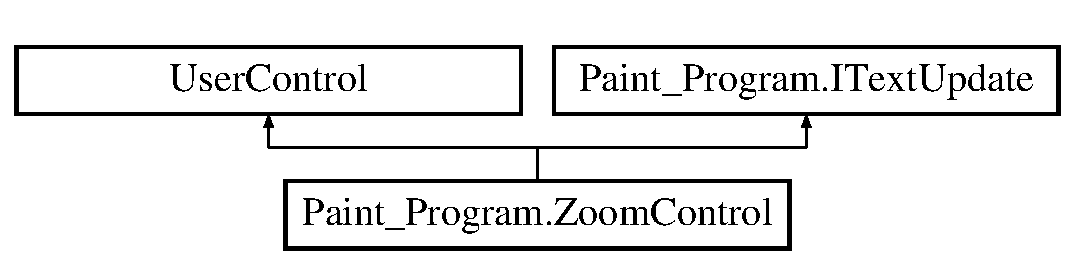
\includegraphics[height=2.000000cm]{class_paint___program_1_1_zoom_control}
\end{center}
\end{figure}
\subsection*{Public Member Functions}
\begin{DoxyCompactItemize}
\item 
\mbox{\hyperlink{class_paint___program_1_1_zoom_control_a7cb51cc074675cf89ce6fd52bf42127a}{Zoom\+Control}} ()
\item 
void \mbox{\hyperlink{class_paint___program_1_1_zoom_control_a2a13fda8b393affa5dfca15d16ce93b8}{set\+Zoom}} (double d)
\item 
double \mbox{\hyperlink{class_paint___program_1_1_zoom_control_ab072d3d242a55e523f64264bd1feccc8}{get\+Zoom\+Percentage}} ()
\item 
double \mbox{\hyperlink{class_paint___program_1_1_zoom_control_a2e0d50a277a9bca1837ca8e11793ecfe}{get\+Zoom\+Factor}} ()
\item 
void \mbox{\hyperlink{class_paint___program_1_1_zoom_control_ab67ee2f3ff5a99c50279ac3b3602a523}{Update\+Text}} ()
\end{DoxyCompactItemize}
\subsection*{Protected Member Functions}
\begin{DoxyCompactItemize}
\item 
override void \mbox{\hyperlink{class_paint___program_1_1_zoom_control_af1161f20c4f21c1852577e26b58720f0}{Dispose}} (bool disposing)
\begin{DoxyCompactList}\small\item\em Clean up any resources being used. \end{DoxyCompactList}\end{DoxyCompactItemize}
\subsection*{Private Member Functions}
\begin{DoxyCompactItemize}
\item 
void \mbox{\hyperlink{class_paint___program_1_1_zoom_control_a1ee526663282fdc5eef952188eba387b}{tb\+Zoom\+\_\+\+Text\+Changed}} (object sender, Event\+Args e)
\item 
void \mbox{\hyperlink{class_paint___program_1_1_zoom_control_a6d2fce455e1f5e4274e5298c3157de5d}{label1\+\_\+\+Click}} (object sender, Event\+Args e)
\item 
void \mbox{\hyperlink{class_paint___program_1_1_zoom_control_a8269532cbb9e59c04a61561c4ae1ebe3}{label2\+\_\+\+Click}} (object sender, Event\+Args e)
\item 
void \mbox{\hyperlink{class_paint___program_1_1_zoom_control_ae61acf927bdaa41820d5ee2c8b5c05c4}{Initialize\+Component}} ()
\begin{DoxyCompactList}\small\item\em Required method for Designer support -\/ do not modify the contents of this method with the code editor. \end{DoxyCompactList}\end{DoxyCompactItemize}
\subsection*{Private Attributes}
\begin{DoxyCompactItemize}
\item 
double \mbox{\hyperlink{class_paint___program_1_1_zoom_control_a929f4269dd2e850603888768d8f83753}{d\+Zoom\+Factor}}
\item 
double \mbox{\hyperlink{class_paint___program_1_1_zoom_control_a615b9941df411c331af5041d38da6ad2}{Z\+O\+O\+M\+\_\+\+M\+IN}} = 1
\item 
const double \mbox{\hyperlink{class_paint___program_1_1_zoom_control_a81f7435ed0a733d8c3fd4d86f5c8e6b2}{Z\+O\+O\+M\+\_\+\+M\+AX}} = 3200
\item 
System.\+Component\+Model.\+I\+Container \mbox{\hyperlink{class_paint___program_1_1_zoom_control_a0c11233497665c39609e490beca6eaf2}{components}} = null
\begin{DoxyCompactList}\small\item\em Required designer variable. \end{DoxyCompactList}\item 
System.\+Windows.\+Forms.\+Label \mbox{\hyperlink{class_paint___program_1_1_zoom_control_af9e86cbd2b21cf273f9c88ca3535cd2e}{l\+Zoom}}
\item 
System.\+Windows.\+Forms.\+Text\+Box \mbox{\hyperlink{class_paint___program_1_1_zoom_control_a1417125b06048606d4075c2f483aea72}{tb\+Zoom}}
\item 
System.\+Windows.\+Forms.\+Label \mbox{\hyperlink{class_paint___program_1_1_zoom_control_ad2e73a7d0623eda78f4483d940f57ed6}{label2}}
\end{DoxyCompactItemize}


\subsection{Constructor \& Destructor Documentation}
\mbox{\Hypertarget{class_paint___program_1_1_zoom_control_a7cb51cc074675cf89ce6fd52bf42127a}\label{class_paint___program_1_1_zoom_control_a7cb51cc074675cf89ce6fd52bf42127a}} 
\index{Paint\+\_\+\+Program\+::\+Zoom\+Control@{Paint\+\_\+\+Program\+::\+Zoom\+Control}!Zoom\+Control@{Zoom\+Control}}
\index{Zoom\+Control@{Zoom\+Control}!Paint\+\_\+\+Program\+::\+Zoom\+Control@{Paint\+\_\+\+Program\+::\+Zoom\+Control}}
\subsubsection{\texorpdfstring{Zoom\+Control()}{ZoomControl()}}
{\footnotesize\ttfamily Paint\+\_\+\+Program.\+Zoom\+Control.\+Zoom\+Control (\begin{DoxyParamCaption}{ }\end{DoxyParamCaption})\hspace{0.3cm}{\ttfamily [inline]}}



\subsection{Member Function Documentation}
\mbox{\Hypertarget{class_paint___program_1_1_zoom_control_af1161f20c4f21c1852577e26b58720f0}\label{class_paint___program_1_1_zoom_control_af1161f20c4f21c1852577e26b58720f0}} 
\index{Paint\+\_\+\+Program\+::\+Zoom\+Control@{Paint\+\_\+\+Program\+::\+Zoom\+Control}!Dispose@{Dispose}}
\index{Dispose@{Dispose}!Paint\+\_\+\+Program\+::\+Zoom\+Control@{Paint\+\_\+\+Program\+::\+Zoom\+Control}}
\subsubsection{\texorpdfstring{Dispose()}{Dispose()}}
{\footnotesize\ttfamily override void Paint\+\_\+\+Program.\+Zoom\+Control.\+Dispose (\begin{DoxyParamCaption}\item[{bool}]{disposing }\end{DoxyParamCaption})\hspace{0.3cm}{\ttfamily [inline]}, {\ttfamily [protected]}}



Clean up any resources being used. 


\begin{DoxyParams}{Parameters}
{\em disposing} & true if managed resources should be disposed; otherwise, false.\\
\hline
\end{DoxyParams}
\mbox{\Hypertarget{class_paint___program_1_1_zoom_control_a2e0d50a277a9bca1837ca8e11793ecfe}\label{class_paint___program_1_1_zoom_control_a2e0d50a277a9bca1837ca8e11793ecfe}} 
\index{Paint\+\_\+\+Program\+::\+Zoom\+Control@{Paint\+\_\+\+Program\+::\+Zoom\+Control}!get\+Zoom\+Factor@{get\+Zoom\+Factor}}
\index{get\+Zoom\+Factor@{get\+Zoom\+Factor}!Paint\+\_\+\+Program\+::\+Zoom\+Control@{Paint\+\_\+\+Program\+::\+Zoom\+Control}}
\subsubsection{\texorpdfstring{get\+Zoom\+Factor()}{getZoomFactor()}}
{\footnotesize\ttfamily double Paint\+\_\+\+Program.\+Zoom\+Control.\+get\+Zoom\+Factor (\begin{DoxyParamCaption}{ }\end{DoxyParamCaption})\hspace{0.3cm}{\ttfamily [inline]}}

\mbox{\Hypertarget{class_paint___program_1_1_zoom_control_ab072d3d242a55e523f64264bd1feccc8}\label{class_paint___program_1_1_zoom_control_ab072d3d242a55e523f64264bd1feccc8}} 
\index{Paint\+\_\+\+Program\+::\+Zoom\+Control@{Paint\+\_\+\+Program\+::\+Zoom\+Control}!get\+Zoom\+Percentage@{get\+Zoom\+Percentage}}
\index{get\+Zoom\+Percentage@{get\+Zoom\+Percentage}!Paint\+\_\+\+Program\+::\+Zoom\+Control@{Paint\+\_\+\+Program\+::\+Zoom\+Control}}
\subsubsection{\texorpdfstring{get\+Zoom\+Percentage()}{getZoomPercentage()}}
{\footnotesize\ttfamily double Paint\+\_\+\+Program.\+Zoom\+Control.\+get\+Zoom\+Percentage (\begin{DoxyParamCaption}{ }\end{DoxyParamCaption})\hspace{0.3cm}{\ttfamily [inline]}}

\mbox{\Hypertarget{class_paint___program_1_1_zoom_control_ae61acf927bdaa41820d5ee2c8b5c05c4}\label{class_paint___program_1_1_zoom_control_ae61acf927bdaa41820d5ee2c8b5c05c4}} 
\index{Paint\+\_\+\+Program\+::\+Zoom\+Control@{Paint\+\_\+\+Program\+::\+Zoom\+Control}!Initialize\+Component@{Initialize\+Component}}
\index{Initialize\+Component@{Initialize\+Component}!Paint\+\_\+\+Program\+::\+Zoom\+Control@{Paint\+\_\+\+Program\+::\+Zoom\+Control}}
\subsubsection{\texorpdfstring{Initialize\+Component()}{InitializeComponent()}}
{\footnotesize\ttfamily void Paint\+\_\+\+Program.\+Zoom\+Control.\+Initialize\+Component (\begin{DoxyParamCaption}{ }\end{DoxyParamCaption})\hspace{0.3cm}{\ttfamily [inline]}, {\ttfamily [private]}}



Required method for Designer support -\/ do not modify the contents of this method with the code editor. 

\mbox{\Hypertarget{class_paint___program_1_1_zoom_control_a6d2fce455e1f5e4274e5298c3157de5d}\label{class_paint___program_1_1_zoom_control_a6d2fce455e1f5e4274e5298c3157de5d}} 
\index{Paint\+\_\+\+Program\+::\+Zoom\+Control@{Paint\+\_\+\+Program\+::\+Zoom\+Control}!label1\+\_\+\+Click@{label1\+\_\+\+Click}}
\index{label1\+\_\+\+Click@{label1\+\_\+\+Click}!Paint\+\_\+\+Program\+::\+Zoom\+Control@{Paint\+\_\+\+Program\+::\+Zoom\+Control}}
\subsubsection{\texorpdfstring{label1\+\_\+\+Click()}{label1\_Click()}}
{\footnotesize\ttfamily void Paint\+\_\+\+Program.\+Zoom\+Control.\+label1\+\_\+\+Click (\begin{DoxyParamCaption}\item[{object}]{sender,  }\item[{Event\+Args}]{e }\end{DoxyParamCaption})\hspace{0.3cm}{\ttfamily [inline]}, {\ttfamily [private]}}

\mbox{\Hypertarget{class_paint___program_1_1_zoom_control_a8269532cbb9e59c04a61561c4ae1ebe3}\label{class_paint___program_1_1_zoom_control_a8269532cbb9e59c04a61561c4ae1ebe3}} 
\index{Paint\+\_\+\+Program\+::\+Zoom\+Control@{Paint\+\_\+\+Program\+::\+Zoom\+Control}!label2\+\_\+\+Click@{label2\+\_\+\+Click}}
\index{label2\+\_\+\+Click@{label2\+\_\+\+Click}!Paint\+\_\+\+Program\+::\+Zoom\+Control@{Paint\+\_\+\+Program\+::\+Zoom\+Control}}
\subsubsection{\texorpdfstring{label2\+\_\+\+Click()}{label2\_Click()}}
{\footnotesize\ttfamily void Paint\+\_\+\+Program.\+Zoom\+Control.\+label2\+\_\+\+Click (\begin{DoxyParamCaption}\item[{object}]{sender,  }\item[{Event\+Args}]{e }\end{DoxyParamCaption})\hspace{0.3cm}{\ttfamily [inline]}, {\ttfamily [private]}}

\mbox{\Hypertarget{class_paint___program_1_1_zoom_control_a2a13fda8b393affa5dfca15d16ce93b8}\label{class_paint___program_1_1_zoom_control_a2a13fda8b393affa5dfca15d16ce93b8}} 
\index{Paint\+\_\+\+Program\+::\+Zoom\+Control@{Paint\+\_\+\+Program\+::\+Zoom\+Control}!set\+Zoom@{set\+Zoom}}
\index{set\+Zoom@{set\+Zoom}!Paint\+\_\+\+Program\+::\+Zoom\+Control@{Paint\+\_\+\+Program\+::\+Zoom\+Control}}
\subsubsection{\texorpdfstring{set\+Zoom()}{setZoom()}}
{\footnotesize\ttfamily void Paint\+\_\+\+Program.\+Zoom\+Control.\+set\+Zoom (\begin{DoxyParamCaption}\item[{double}]{d }\end{DoxyParamCaption})\hspace{0.3cm}{\ttfamily [inline]}}

\mbox{\Hypertarget{class_paint___program_1_1_zoom_control_a1ee526663282fdc5eef952188eba387b}\label{class_paint___program_1_1_zoom_control_a1ee526663282fdc5eef952188eba387b}} 
\index{Paint\+\_\+\+Program\+::\+Zoom\+Control@{Paint\+\_\+\+Program\+::\+Zoom\+Control}!tb\+Zoom\+\_\+\+Text\+Changed@{tb\+Zoom\+\_\+\+Text\+Changed}}
\index{tb\+Zoom\+\_\+\+Text\+Changed@{tb\+Zoom\+\_\+\+Text\+Changed}!Paint\+\_\+\+Program\+::\+Zoom\+Control@{Paint\+\_\+\+Program\+::\+Zoom\+Control}}
\subsubsection{\texorpdfstring{tb\+Zoom\+\_\+\+Text\+Changed()}{tbZoom\_TextChanged()}}
{\footnotesize\ttfamily void Paint\+\_\+\+Program.\+Zoom\+Control.\+tb\+Zoom\+\_\+\+Text\+Changed (\begin{DoxyParamCaption}\item[{object}]{sender,  }\item[{Event\+Args}]{e }\end{DoxyParamCaption})\hspace{0.3cm}{\ttfamily [inline]}, {\ttfamily [private]}}

\mbox{\Hypertarget{class_paint___program_1_1_zoom_control_ab67ee2f3ff5a99c50279ac3b3602a523}\label{class_paint___program_1_1_zoom_control_ab67ee2f3ff5a99c50279ac3b3602a523}} 
\index{Paint\+\_\+\+Program\+::\+Zoom\+Control@{Paint\+\_\+\+Program\+::\+Zoom\+Control}!Update\+Text@{Update\+Text}}
\index{Update\+Text@{Update\+Text}!Paint\+\_\+\+Program\+::\+Zoom\+Control@{Paint\+\_\+\+Program\+::\+Zoom\+Control}}
\subsubsection{\texorpdfstring{Update\+Text()}{UpdateText()}}
{\footnotesize\ttfamily void Paint\+\_\+\+Program.\+Zoom\+Control.\+Update\+Text (\begin{DoxyParamCaption}{ }\end{DoxyParamCaption})\hspace{0.3cm}{\ttfamily [inline]}}



Implements \mbox{\hyperlink{interface_paint___program_1_1_i_text_update_ad1e94db137571608917117e9a6f7479b}{Paint\+\_\+\+Program.\+I\+Text\+Update}}.



\subsection{Member Data Documentation}
\mbox{\Hypertarget{class_paint___program_1_1_zoom_control_a0c11233497665c39609e490beca6eaf2}\label{class_paint___program_1_1_zoom_control_a0c11233497665c39609e490beca6eaf2}} 
\index{Paint\+\_\+\+Program\+::\+Zoom\+Control@{Paint\+\_\+\+Program\+::\+Zoom\+Control}!components@{components}}
\index{components@{components}!Paint\+\_\+\+Program\+::\+Zoom\+Control@{Paint\+\_\+\+Program\+::\+Zoom\+Control}}
\subsubsection{\texorpdfstring{components}{components}}
{\footnotesize\ttfamily System.\+Component\+Model.\+I\+Container Paint\+\_\+\+Program.\+Zoom\+Control.\+components = null\hspace{0.3cm}{\ttfamily [private]}}



Required designer variable. 

\mbox{\Hypertarget{class_paint___program_1_1_zoom_control_a929f4269dd2e850603888768d8f83753}\label{class_paint___program_1_1_zoom_control_a929f4269dd2e850603888768d8f83753}} 
\index{Paint\+\_\+\+Program\+::\+Zoom\+Control@{Paint\+\_\+\+Program\+::\+Zoom\+Control}!d\+Zoom\+Factor@{d\+Zoom\+Factor}}
\index{d\+Zoom\+Factor@{d\+Zoom\+Factor}!Paint\+\_\+\+Program\+::\+Zoom\+Control@{Paint\+\_\+\+Program\+::\+Zoom\+Control}}
\subsubsection{\texorpdfstring{d\+Zoom\+Factor}{dZoomFactor}}
{\footnotesize\ttfamily double Paint\+\_\+\+Program.\+Zoom\+Control.\+d\+Zoom\+Factor\hspace{0.3cm}{\ttfamily [private]}}

\mbox{\Hypertarget{class_paint___program_1_1_zoom_control_ad2e73a7d0623eda78f4483d940f57ed6}\label{class_paint___program_1_1_zoom_control_ad2e73a7d0623eda78f4483d940f57ed6}} 
\index{Paint\+\_\+\+Program\+::\+Zoom\+Control@{Paint\+\_\+\+Program\+::\+Zoom\+Control}!label2@{label2}}
\index{label2@{label2}!Paint\+\_\+\+Program\+::\+Zoom\+Control@{Paint\+\_\+\+Program\+::\+Zoom\+Control}}
\subsubsection{\texorpdfstring{label2}{label2}}
{\footnotesize\ttfamily System.\+Windows.\+Forms.\+Label Paint\+\_\+\+Program.\+Zoom\+Control.\+label2\hspace{0.3cm}{\ttfamily [private]}}

\mbox{\Hypertarget{class_paint___program_1_1_zoom_control_af9e86cbd2b21cf273f9c88ca3535cd2e}\label{class_paint___program_1_1_zoom_control_af9e86cbd2b21cf273f9c88ca3535cd2e}} 
\index{Paint\+\_\+\+Program\+::\+Zoom\+Control@{Paint\+\_\+\+Program\+::\+Zoom\+Control}!l\+Zoom@{l\+Zoom}}
\index{l\+Zoom@{l\+Zoom}!Paint\+\_\+\+Program\+::\+Zoom\+Control@{Paint\+\_\+\+Program\+::\+Zoom\+Control}}
\subsubsection{\texorpdfstring{l\+Zoom}{lZoom}}
{\footnotesize\ttfamily System.\+Windows.\+Forms.\+Label Paint\+\_\+\+Program.\+Zoom\+Control.\+l\+Zoom\hspace{0.3cm}{\ttfamily [private]}}

\mbox{\Hypertarget{class_paint___program_1_1_zoom_control_a1417125b06048606d4075c2f483aea72}\label{class_paint___program_1_1_zoom_control_a1417125b06048606d4075c2f483aea72}} 
\index{Paint\+\_\+\+Program\+::\+Zoom\+Control@{Paint\+\_\+\+Program\+::\+Zoom\+Control}!tb\+Zoom@{tb\+Zoom}}
\index{tb\+Zoom@{tb\+Zoom}!Paint\+\_\+\+Program\+::\+Zoom\+Control@{Paint\+\_\+\+Program\+::\+Zoom\+Control}}
\subsubsection{\texorpdfstring{tb\+Zoom}{tbZoom}}
{\footnotesize\ttfamily System.\+Windows.\+Forms.\+Text\+Box Paint\+\_\+\+Program.\+Zoom\+Control.\+tb\+Zoom\hspace{0.3cm}{\ttfamily [private]}}

\mbox{\Hypertarget{class_paint___program_1_1_zoom_control_a81f7435ed0a733d8c3fd4d86f5c8e6b2}\label{class_paint___program_1_1_zoom_control_a81f7435ed0a733d8c3fd4d86f5c8e6b2}} 
\index{Paint\+\_\+\+Program\+::\+Zoom\+Control@{Paint\+\_\+\+Program\+::\+Zoom\+Control}!Z\+O\+O\+M\+\_\+\+M\+AX@{Z\+O\+O\+M\+\_\+\+M\+AX}}
\index{Z\+O\+O\+M\+\_\+\+M\+AX@{Z\+O\+O\+M\+\_\+\+M\+AX}!Paint\+\_\+\+Program\+::\+Zoom\+Control@{Paint\+\_\+\+Program\+::\+Zoom\+Control}}
\subsubsection{\texorpdfstring{Z\+O\+O\+M\+\_\+\+M\+AX}{ZOOM\_MAX}}
{\footnotesize\ttfamily const double Paint\+\_\+\+Program.\+Zoom\+Control.\+Z\+O\+O\+M\+\_\+\+M\+AX = 3200\hspace{0.3cm}{\ttfamily [private]}}

\mbox{\Hypertarget{class_paint___program_1_1_zoom_control_a615b9941df411c331af5041d38da6ad2}\label{class_paint___program_1_1_zoom_control_a615b9941df411c331af5041d38da6ad2}} 
\index{Paint\+\_\+\+Program\+::\+Zoom\+Control@{Paint\+\_\+\+Program\+::\+Zoom\+Control}!Z\+O\+O\+M\+\_\+\+M\+IN@{Z\+O\+O\+M\+\_\+\+M\+IN}}
\index{Z\+O\+O\+M\+\_\+\+M\+IN@{Z\+O\+O\+M\+\_\+\+M\+IN}!Paint\+\_\+\+Program\+::\+Zoom\+Control@{Paint\+\_\+\+Program\+::\+Zoom\+Control}}
\subsubsection{\texorpdfstring{Z\+O\+O\+M\+\_\+\+M\+IN}{ZOOM\_MIN}}
{\footnotesize\ttfamily double Paint\+\_\+\+Program.\+Zoom\+Control.\+Z\+O\+O\+M\+\_\+\+M\+IN = 1\hspace{0.3cm}{\ttfamily [private]}}



The documentation for this class was generated from the following files\+:\begin{DoxyCompactItemize}
\item 
Paint Program/\mbox{\hyperlink{_zoom_control_8cs}{Zoom\+Control.\+cs}}\item 
Paint Program/\mbox{\hyperlink{_zoom_control_8_designer_8cs}{Zoom\+Control.\+Designer.\+cs}}\end{DoxyCompactItemize}

\chapter{File Documentation}
\hypertarget{_brush_settings_8cs}{}\section{Paint Program/\+Brush\+Settings.cs File Reference}
\label{_brush_settings_8cs}\index{Paint Program/\+Brush\+Settings.\+cs@{Paint Program/\+Brush\+Settings.\+cs}}
\subsection*{Classes}
\begin{DoxyCompactItemize}
\item 
class \mbox{\hyperlink{class_paint___program_1_1_brush_settings}{Paint\+\_\+\+Program.\+Brush\+Settings}}
\end{DoxyCompactItemize}
\subsection*{Namespaces}
\begin{DoxyCompactItemize}
\item 
namespace \mbox{\hyperlink{namespace_paint___program}{Paint\+\_\+\+Program}}
\end{DoxyCompactItemize}

\hypertarget{_brush_settings_8_designer_8cs}{}\section{Paint Program/\+Brush\+Settings.Designer.\+cs File Reference}
\label{_brush_settings_8_designer_8cs}\index{Paint Program/\+Brush\+Settings.\+Designer.\+cs@{Paint Program/\+Brush\+Settings.\+Designer.\+cs}}
\subsection*{Classes}
\begin{DoxyCompactItemize}
\item 
class \mbox{\hyperlink{class_paint___program_1_1_brush_settings}{Paint\+\_\+\+Program.\+Brush\+Settings}}
\end{DoxyCompactItemize}
\subsection*{Namespaces}
\begin{DoxyCompactItemize}
\item 
namespace \mbox{\hyperlink{namespace_paint___program}{Paint\+\_\+\+Program}}
\end{DoxyCompactItemize}

\hypertarget{_brush_tool_8cs}{}\section{Paint Program/\+Brush\+Tool.cs File Reference}
\label{_brush_tool_8cs}\index{Paint Program/\+Brush\+Tool.\+cs@{Paint Program/\+Brush\+Tool.\+cs}}
\subsection*{Classes}
\begin{DoxyCompactItemize}
\item 
class \mbox{\hyperlink{class_paint___program_1_1_brush_tool}{Paint\+\_\+\+Program.\+Brush\+Tool}}
\end{DoxyCompactItemize}
\subsection*{Namespaces}
\begin{DoxyCompactItemize}
\item 
namespace \mbox{\hyperlink{namespace_paint___program}{Paint\+\_\+\+Program}}
\end{DoxyCompactItemize}

\hypertarget{_canvas_8cs}{}\section{Paint Program/\+Canvas.cs File Reference}
\label{_canvas_8cs}\index{Paint Program/\+Canvas.\+cs@{Paint Program/\+Canvas.\+cs}}
\subsection*{Classes}
\begin{DoxyCompactItemize}
\item 
class \mbox{\hyperlink{class_paint___program_1_1_canvas}{Paint\+\_\+\+Program.\+Canvas}}
\begin{DoxyCompactList}\small\item\em Class handling the main rendering of the layers, and interfacing with tools \end{DoxyCompactList}\end{DoxyCompactItemize}
\subsection*{Namespaces}
\begin{DoxyCompactItemize}
\item 
namespace \mbox{\hyperlink{namespace_paint___program}{Paint\+\_\+\+Program}}
\end{DoxyCompactItemize}

\hypertarget{_canvas_8_designer_8cs}{}\section{Paint Program/\+Canvas.Designer.\+cs File Reference}
\label{_canvas_8_designer_8cs}\index{Paint Program/\+Canvas.\+Designer.\+cs@{Paint Program/\+Canvas.\+Designer.\+cs}}
\subsection*{Classes}
\begin{DoxyCompactItemize}
\item 
class \mbox{\hyperlink{class_paint___program_1_1_canvas}{Paint\+\_\+\+Program.\+Canvas}}
\begin{DoxyCompactList}\small\item\em Class handling the main rendering of the layers, and interfacing with tools \end{DoxyCompactList}\end{DoxyCompactItemize}
\subsection*{Namespaces}
\begin{DoxyCompactItemize}
\item 
namespace \mbox{\hyperlink{namespace_paint___program}{Paint\+\_\+\+Program}}
\end{DoxyCompactItemize}

\hypertarget{_color_sampling_tool_8cs}{}\section{Paint Program/\+Color\+Sampling\+Tool.cs File Reference}
\label{_color_sampling_tool_8cs}\index{Paint Program/\+Color\+Sampling\+Tool.\+cs@{Paint Program/\+Color\+Sampling\+Tool.\+cs}}
\subsection*{Classes}
\begin{DoxyCompactItemize}
\item 
class \mbox{\hyperlink{class_paint___program_1_1_color_sampling_tool}{Paint\+\_\+\+Program.\+Color\+Sampling\+Tool}}
\end{DoxyCompactItemize}
\subsection*{Namespaces}
\begin{DoxyCompactItemize}
\item 
namespace \mbox{\hyperlink{namespace_paint___program}{Paint\+\_\+\+Program}}
\end{DoxyCompactItemize}

\hypertarget{_debug_tool_8cs}{}\section{Paint Program/\+Debug\+Tool.cs File Reference}
\label{_debug_tool_8cs}\index{Paint Program/\+Debug\+Tool.\+cs@{Paint Program/\+Debug\+Tool.\+cs}}
\subsection*{Classes}
\begin{DoxyCompactItemize}
\item 
class \mbox{\hyperlink{class_paint___program_1_1_debug_tool}{Paint\+\_\+\+Program.\+Debug\+Tool}}
\begin{DoxyCompactList}\small\item\em Debug class, please ignore \end{DoxyCompactList}\end{DoxyCompactItemize}
\subsection*{Namespaces}
\begin{DoxyCompactItemize}
\item 
namespace \mbox{\hyperlink{namespace_paint___program}{Paint\+\_\+\+Program}}
\end{DoxyCompactItemize}

\hypertarget{_display_8cs}{}\section{Paint Program/\+Display.cs File Reference}
\label{_display_8cs}\index{Paint Program/\+Display.\+cs@{Paint Program/\+Display.\+cs}}
\subsection*{Classes}
\begin{DoxyCompactItemize}
\item 
class \mbox{\hyperlink{class_paint___program_1_1_display}{Paint\+\_\+\+Program.\+Display}}
\end{DoxyCompactItemize}
\subsection*{Namespaces}
\begin{DoxyCompactItemize}
\item 
namespace \mbox{\hyperlink{namespace_paint___program}{Paint\+\_\+\+Program}}
\end{DoxyCompactItemize}

\hypertarget{_eraser_tool_8cs}{}\section{Paint Program/\+Eraser\+Tool.cs File Reference}
\label{_eraser_tool_8cs}\index{Paint Program/\+Eraser\+Tool.\+cs@{Paint Program/\+Eraser\+Tool.\+cs}}
\subsection*{Classes}
\begin{DoxyCompactItemize}
\item 
class \mbox{\hyperlink{class_paint___program_1_1_eraser_tool}{Paint\+\_\+\+Program.\+Eraser\+Tool}}
\end{DoxyCompactItemize}
\subsection*{Namespaces}
\begin{DoxyCompactItemize}
\item 
namespace \mbox{\hyperlink{namespace_paint___program}{Paint\+\_\+\+Program}}
\end{DoxyCompactItemize}

\hypertarget{_file_save_8cs}{}\section{Paint Program/\+File\+Save.cs File Reference}
\label{_file_save_8cs}\index{Paint Program/\+File\+Save.\+cs@{Paint Program/\+File\+Save.\+cs}}
\subsection*{Classes}
\begin{DoxyCompactItemize}
\item 
class \mbox{\hyperlink{class_paint___program_1_1_file_save}{Paint\+\_\+\+Program.\+File\+Save}}
\end{DoxyCompactItemize}
\subsection*{Namespaces}
\begin{DoxyCompactItemize}
\item 
namespace \mbox{\hyperlink{namespace_paint___program}{Paint\+\_\+\+Program}}
\end{DoxyCompactItemize}

\hypertarget{_form1_8cs}{}\section{Paint Program/\+Form1.cs File Reference}
\label{_form1_8cs}\index{Paint Program/\+Form1.\+cs@{Paint Program/\+Form1.\+cs}}
\subsection*{Classes}
\begin{DoxyCompactItemize}
\item 
class \mbox{\hyperlink{class_paint___program_1_1_form1}{Paint\+\_\+\+Program.\+Form1}}
\end{DoxyCompactItemize}
\subsection*{Namespaces}
\begin{DoxyCompactItemize}
\item 
namespace \mbox{\hyperlink{namespace_paint___program}{Paint\+\_\+\+Program}}
\end{DoxyCompactItemize}

\hypertarget{_form1_8_designer_8cs}{}\section{Paint Program/\+Form1.Designer.\+cs File Reference}
\label{_form1_8_designer_8cs}\index{Paint Program/\+Form1.\+Designer.\+cs@{Paint Program/\+Form1.\+Designer.\+cs}}
\subsection*{Classes}
\begin{DoxyCompactItemize}
\item 
class \mbox{\hyperlink{class_paint___program_1_1_form1}{Paint\+\_\+\+Program.\+Form1}}
\end{DoxyCompactItemize}
\subsection*{Namespaces}
\begin{DoxyCompactItemize}
\item 
namespace \mbox{\hyperlink{namespace_paint___program}{Paint\+\_\+\+Program}}
\end{DoxyCompactItemize}

\hypertarget{_g_drive_save_dialog_8cs}{}\section{Paint Program/\+G\+Drive\+Save\+Dialog.cs File Reference}
\label{_g_drive_save_dialog_8cs}\index{Paint Program/\+G\+Drive\+Save\+Dialog.\+cs@{Paint Program/\+G\+Drive\+Save\+Dialog.\+cs}}
\subsection*{Classes}
\begin{DoxyCompactItemize}
\item 
class \mbox{\hyperlink{class_paint___program_1_1_g_drive_save_dialog}{Paint\+\_\+\+Program.\+G\+Drive\+Save\+Dialog}}
\end{DoxyCompactItemize}
\subsection*{Namespaces}
\begin{DoxyCompactItemize}
\item 
namespace \mbox{\hyperlink{namespace_paint___program}{Paint\+\_\+\+Program}}
\end{DoxyCompactItemize}

\hypertarget{_g_drive_save_dialog_8_designer_8cs}{}\section{Paint Program/\+G\+Drive\+Save\+Dialog.Designer.\+cs File Reference}
\label{_g_drive_save_dialog_8_designer_8cs}\index{Paint Program/\+G\+Drive\+Save\+Dialog.\+Designer.\+cs@{Paint Program/\+G\+Drive\+Save\+Dialog.\+Designer.\+cs}}
\subsection*{Classes}
\begin{DoxyCompactItemize}
\item 
class \mbox{\hyperlink{class_paint___program_1_1_g_drive_save_dialog}{Paint\+\_\+\+Program.\+G\+Drive\+Save\+Dialog}}
\end{DoxyCompactItemize}
\subsection*{Namespaces}
\begin{DoxyCompactItemize}
\item 
namespace \mbox{\hyperlink{namespace_paint___program}{Paint\+\_\+\+Program}}
\end{DoxyCompactItemize}

\hypertarget{_gif_encoder_8cs}{}\section{Paint Program/\+Gif\+Encoder.cs File Reference}
\label{_gif_encoder_8cs}\index{Paint Program/\+Gif\+Encoder.\+cs@{Paint Program/\+Gif\+Encoder.\+cs}}
\subsection*{Classes}
\begin{DoxyCompactItemize}
\item 
class \mbox{\hyperlink{class_paint___program_1_1_gif_encoder}{Paint\+\_\+\+Program.\+Gif\+Encoder}}
\begin{DoxyCompactList}\small\item\em Encodes multiple images as an animated gif to a stream. ~\newline
 A\+L\+W\+A\+YS A\+L\+W\+A\+YS A\+L\+W\+A\+YS wire this up in a using block ~\newline
 Disposing the encoder will complete the file. ~\newline
 Uses default .net G\+IF encoding and adds animation headers. \end{DoxyCompactList}\end{DoxyCompactItemize}
\subsection*{Namespaces}
\begin{DoxyCompactItemize}
\item 
namespace \mbox{\hyperlink{namespace_paint___program}{Paint\+\_\+\+Program}}
\end{DoxyCompactItemize}

\hypertarget{_google_drive_upload_8cs}{}\section{Paint Program/\+Google\+Drive\+Upload.cs File Reference}
\label{_google_drive_upload_8cs}\index{Paint Program/\+Google\+Drive\+Upload.\+cs@{Paint Program/\+Google\+Drive\+Upload.\+cs}}
\subsection*{Classes}
\begin{DoxyCompactItemize}
\item 
class \mbox{\hyperlink{class_paint___program_1_1_google_drive_upload}{Paint\+\_\+\+Program.\+Google\+Drive\+Upload}}
\end{DoxyCompactItemize}
\subsection*{Namespaces}
\begin{DoxyCompactItemize}
\item 
namespace \mbox{\hyperlink{namespace_paint___program}{Paint\+\_\+\+Program}}
\end{DoxyCompactItemize}

\hypertarget{_green_screen_tool_8cs}{}\section{Paint Program/\+Green\+Screen\+Tool.cs File Reference}
\label{_green_screen_tool_8cs}\index{Paint Program/\+Green\+Screen\+Tool.\+cs@{Paint Program/\+Green\+Screen\+Tool.\+cs}}
\subsection*{Classes}
\begin{DoxyCompactItemize}
\item 
class \mbox{\hyperlink{class_paint___program_1_1_green_screen_tool}{Paint\+\_\+\+Program.\+Green\+Screen\+Tool}}
\end{DoxyCompactItemize}
\subsection*{Namespaces}
\begin{DoxyCompactItemize}
\item 
namespace \mbox{\hyperlink{namespace_paint___program}{Paint\+\_\+\+Program}}
\end{DoxyCompactItemize}

\hypertarget{_image_import_8cs}{}\section{Paint Program/\+Image\+Import.cs File Reference}
\label{_image_import_8cs}\index{Paint Program/\+Image\+Import.\+cs@{Paint Program/\+Image\+Import.\+cs}}
\subsection*{Classes}
\begin{DoxyCompactItemize}
\item 
class \mbox{\hyperlink{class_paint___program_1_1_image_import}{Paint\+\_\+\+Program.\+Image\+Import}}
\end{DoxyCompactItemize}
\subsection*{Namespaces}
\begin{DoxyCompactItemize}
\item 
namespace \mbox{\hyperlink{namespace_paint___program}{Paint\+\_\+\+Program}}
\end{DoxyCompactItemize}

\hypertarget{_i_text_update_8cs}{}\section{Paint Program/\+I\+Text\+Update.cs File Reference}
\label{_i_text_update_8cs}\index{Paint Program/\+I\+Text\+Update.\+cs@{Paint Program/\+I\+Text\+Update.\+cs}}
\subsection*{Classes}
\begin{DoxyCompactItemize}
\item 
interface \mbox{\hyperlink{interface_paint___program_1_1_i_text_update}{Paint\+\_\+\+Program.\+I\+Text\+Update}}
\end{DoxyCompactItemize}
\subsection*{Namespaces}
\begin{DoxyCompactItemize}
\item 
namespace \mbox{\hyperlink{namespace_paint___program}{Paint\+\_\+\+Program}}
\end{DoxyCompactItemize}

\hypertarget{_i_tool_8cs}{}\section{Paint Program/\+I\+Tool.cs File Reference}
\label{_i_tool_8cs}\index{Paint Program/\+I\+Tool.\+cs@{Paint Program/\+I\+Tool.\+cs}}
\subsection*{Classes}
\begin{DoxyCompactItemize}
\item 
interface \mbox{\hyperlink{interface_paint___program_1_1_i_tool}{Paint\+\_\+\+Program.\+I\+Tool}}
\end{DoxyCompactItemize}
\subsection*{Namespaces}
\begin{DoxyCompactItemize}
\item 
namespace \mbox{\hyperlink{namespace_paint___program}{Paint\+\_\+\+Program}}
\end{DoxyCompactItemize}

\hypertarget{_layer_item_8cs}{}\section{Paint Program/\+Layer\+Item.cs File Reference}
\label{_layer_item_8cs}\index{Paint Program/\+Layer\+Item.\+cs@{Paint Program/\+Layer\+Item.\+cs}}
\subsection*{Classes}
\begin{DoxyCompactItemize}
\item 
class \mbox{\hyperlink{class_paint___program_1_1_layer_item}{Paint\+\_\+\+Program.\+Layer\+Item}}
\end{DoxyCompactItemize}
\subsection*{Namespaces}
\begin{DoxyCompactItemize}
\item 
namespace \mbox{\hyperlink{namespace_paint___program}{Paint\+\_\+\+Program}}
\end{DoxyCompactItemize}

\hypertarget{_layer_item_8_designer_8cs}{}\section{Paint Program/\+Layer\+Item.Designer.\+cs File Reference}
\label{_layer_item_8_designer_8cs}\index{Paint Program/\+Layer\+Item.\+Designer.\+cs@{Paint Program/\+Layer\+Item.\+Designer.\+cs}}
\subsection*{Classes}
\begin{DoxyCompactItemize}
\item 
class \mbox{\hyperlink{class_paint___program_1_1_layer_item}{Paint\+\_\+\+Program.\+Layer\+Item}}
\end{DoxyCompactItemize}
\subsection*{Namespaces}
\begin{DoxyCompactItemize}
\item 
namespace \mbox{\hyperlink{namespace_paint___program}{Paint\+\_\+\+Program}}
\end{DoxyCompactItemize}

\hypertarget{_layer_view_8cs}{}\section{Paint Program/\+Layer\+View.cs File Reference}
\label{_layer_view_8cs}\index{Paint Program/\+Layer\+View.\+cs@{Paint Program/\+Layer\+View.\+cs}}
\subsection*{Classes}
\begin{DoxyCompactItemize}
\item 
class \mbox{\hyperlink{class_paint___program_1_1_layer_view}{Paint\+\_\+\+Program.\+Layer\+View}}
\end{DoxyCompactItemize}
\subsection*{Namespaces}
\begin{DoxyCompactItemize}
\item 
namespace \mbox{\hyperlink{namespace_paint___program}{Paint\+\_\+\+Program}}
\end{DoxyCompactItemize}

\hypertarget{_layer_view_8_designer_8cs}{}\section{Paint Program/\+Layer\+View.Designer.\+cs File Reference}
\label{_layer_view_8_designer_8cs}\index{Paint Program/\+Layer\+View.\+Designer.\+cs@{Paint Program/\+Layer\+View.\+Designer.\+cs}}
\subsection*{Classes}
\begin{DoxyCompactItemize}
\item 
class \mbox{\hyperlink{class_paint___program_1_1_layer_view}{Paint\+\_\+\+Program.\+Layer\+View}}
\end{DoxyCompactItemize}
\subsection*{Namespaces}
\begin{DoxyCompactItemize}
\item 
namespace \mbox{\hyperlink{namespace_paint___program}{Paint\+\_\+\+Program}}
\end{DoxyCompactItemize}

\hypertarget{_move_tool_8cs}{}\section{Paint Program/\+Move\+Tool.cs File Reference}
\label{_move_tool_8cs}\index{Paint Program/\+Move\+Tool.\+cs@{Paint Program/\+Move\+Tool.\+cs}}
\subsection*{Classes}
\begin{DoxyCompactItemize}
\item 
class \mbox{\hyperlink{class_paint___program_1_1_move_tool}{Paint\+\_\+\+Program.\+Move\+Tool}}
\end{DoxyCompactItemize}
\subsection*{Namespaces}
\begin{DoxyCompactItemize}
\item 
namespace \mbox{\hyperlink{namespace_paint___program}{Paint\+\_\+\+Program}}
\end{DoxyCompactItemize}

\hypertarget{_new_project_form_8cs}{}\section{Paint Program/\+New\+Project\+Form.cs File Reference}
\label{_new_project_form_8cs}\index{Paint Program/\+New\+Project\+Form.\+cs@{Paint Program/\+New\+Project\+Form.\+cs}}
\subsection*{Classes}
\begin{DoxyCompactItemize}
\item 
class \mbox{\hyperlink{class_paint___program_1_1_new_project_form}{Paint\+\_\+\+Program.\+New\+Project\+Form}}
\end{DoxyCompactItemize}
\subsection*{Namespaces}
\begin{DoxyCompactItemize}
\item 
namespace \mbox{\hyperlink{namespace_paint___program}{Paint\+\_\+\+Program}}
\end{DoxyCompactItemize}

\hypertarget{_new_project_form_8_designer_8cs}{}\section{Paint Program/\+New\+Project\+Form.Designer.\+cs File Reference}
\label{_new_project_form_8_designer_8cs}\index{Paint Program/\+New\+Project\+Form.\+Designer.\+cs@{Paint Program/\+New\+Project\+Form.\+Designer.\+cs}}
\subsection*{Classes}
\begin{DoxyCompactItemize}
\item 
class \mbox{\hyperlink{class_paint___program_1_1_new_project_form}{Paint\+\_\+\+Program.\+New\+Project\+Form}}
\end{DoxyCompactItemize}
\subsection*{Namespaces}
\begin{DoxyCompactItemize}
\item 
namespace \mbox{\hyperlink{namespace_paint___program}{Paint\+\_\+\+Program}}
\end{DoxyCompactItemize}

\hypertarget{_paint_bucket_tool_8cs}{}\section{Paint Program/\+Paint\+Bucket\+Tool.cs File Reference}
\label{_paint_bucket_tool_8cs}\index{Paint Program/\+Paint\+Bucket\+Tool.\+cs@{Paint Program/\+Paint\+Bucket\+Tool.\+cs}}
\subsection*{Classes}
\begin{DoxyCompactItemize}
\item 
class \mbox{\hyperlink{class_paint___program_1_1_paint_bucket_tool}{Paint\+\_\+\+Program.\+Paint\+Bucket\+Tool}}
\end{DoxyCompactItemize}
\subsection*{Namespaces}
\begin{DoxyCompactItemize}
\item 
namespace \mbox{\hyperlink{namespace_paint___program}{Paint\+\_\+\+Program}}
\end{DoxyCompactItemize}

\hypertarget{_pencil_tool_8cs}{}\section{Paint Program/\+Pencil\+Tool.cs File Reference}
\label{_pencil_tool_8cs}\index{Paint Program/\+Pencil\+Tool.\+cs@{Paint Program/\+Pencil\+Tool.\+cs}}
\subsection*{Classes}
\begin{DoxyCompactItemize}
\item 
class \mbox{\hyperlink{class_paint___program_1_1_pencil_tool}{Paint\+\_\+\+Program.\+Pencil\+Tool}}
\end{DoxyCompactItemize}
\subsection*{Namespaces}
\begin{DoxyCompactItemize}
\item 
namespace \mbox{\hyperlink{namespace_paint___program}{Paint\+\_\+\+Program}}
\end{DoxyCompactItemize}

\hypertarget{_program_8cs}{}\section{Paint Program/\+Program.cs File Reference}
\label{_program_8cs}\index{Paint Program/\+Program.\+cs@{Paint Program/\+Program.\+cs}}
\subsection*{Classes}
\begin{DoxyCompactItemize}
\item 
class \mbox{\hyperlink{class_paint___program_1_1_program}{Paint\+\_\+\+Program.\+Program}}
\end{DoxyCompactItemize}
\subsection*{Namespaces}
\begin{DoxyCompactItemize}
\item 
namespace \mbox{\hyperlink{namespace_paint___program}{Paint\+\_\+\+Program}}
\end{DoxyCompactItemize}

\hypertarget{_project_load_8cs}{}\section{Paint Program/\+Project\+Load.cs File Reference}
\label{_project_load_8cs}\index{Paint Program/\+Project\+Load.\+cs@{Paint Program/\+Project\+Load.\+cs}}
\subsection*{Classes}
\begin{DoxyCompactItemize}
\item 
class \mbox{\hyperlink{class_paint___program_1_1_project_load}{Paint\+\_\+\+Program.\+Project\+Load}}
\end{DoxyCompactItemize}
\subsection*{Namespaces}
\begin{DoxyCompactItemize}
\item 
namespace \mbox{\hyperlink{namespace_paint___program}{Paint\+\_\+\+Program}}
\end{DoxyCompactItemize}

\hypertarget{_project_save_8cs}{}\section{Paint Program/\+Project\+Save.cs File Reference}
\label{_project_save_8cs}\index{Paint Program/\+Project\+Save.\+cs@{Paint Program/\+Project\+Save.\+cs}}
\subsection*{Classes}
\begin{DoxyCompactItemize}
\item 
class \mbox{\hyperlink{class_paint___program_1_1_project_save}{Paint\+\_\+\+Program.\+Project\+Save}}
\end{DoxyCompactItemize}
\subsection*{Namespaces}
\begin{DoxyCompactItemize}
\item 
namespace \mbox{\hyperlink{namespace_paint___program}{Paint\+\_\+\+Program}}
\end{DoxyCompactItemize}

\hypertarget{_save_to_drive_8cs}{}\section{Paint Program/\+Save\+To\+Drive.cs File Reference}
\label{_save_to_drive_8cs}\index{Paint Program/\+Save\+To\+Drive.\+cs@{Paint Program/\+Save\+To\+Drive.\+cs}}
\subsection*{Classes}
\begin{DoxyCompactItemize}
\item 
class \mbox{\hyperlink{class_paint___program_1_1_save_to_drive}{Paint\+\_\+\+Program.\+Save\+To\+Drive}}
\end{DoxyCompactItemize}
\subsection*{Namespaces}
\begin{DoxyCompactItemize}
\item 
namespace \mbox{\hyperlink{namespace_paint___program}{Paint\+\_\+\+Program}}
\end{DoxyCompactItemize}

\hypertarget{_selection_tool_8cs}{}\section{Paint Program/\+Selection\+Tool.cs File Reference}
\label{_selection_tool_8cs}\index{Paint Program/\+Selection\+Tool.\+cs@{Paint Program/\+Selection\+Tool.\+cs}}
\subsection*{Classes}
\begin{DoxyCompactItemize}
\item 
class \mbox{\hyperlink{class_paint___program_1_1_selection_tool}{Paint\+\_\+\+Program.\+Selection\+Tool}}
\end{DoxyCompactItemize}
\subsection*{Namespaces}
\begin{DoxyCompactItemize}
\item 
namespace \mbox{\hyperlink{namespace_paint___program}{Paint\+\_\+\+Program}}
\end{DoxyCompactItemize}

\hypertarget{_shared_settings_8cs}{}\section{Paint Program/\+Shared\+Settings.cs File Reference}
\label{_shared_settings_8cs}\index{Paint Program/\+Shared\+Settings.\+cs@{Paint Program/\+Shared\+Settings.\+cs}}
\subsection*{Classes}
\begin{DoxyCompactItemize}
\item 
class \mbox{\hyperlink{class_paint___program_1_1_shared_settings}{Paint\+\_\+\+Program.\+Shared\+Settings}}
\end{DoxyCompactItemize}
\subsection*{Namespaces}
\begin{DoxyCompactItemize}
\item 
namespace \mbox{\hyperlink{namespace_paint___program}{Paint\+\_\+\+Program}}
\end{DoxyCompactItemize}

\hypertarget{_straight_line_tool_8cs}{}\section{Paint Program/\+Straight\+Line\+Tool.cs File Reference}
\label{_straight_line_tool_8cs}\index{Paint Program/\+Straight\+Line\+Tool.\+cs@{Paint Program/\+Straight\+Line\+Tool.\+cs}}
\subsection*{Classes}
\begin{DoxyCompactItemize}
\item 
class \mbox{\hyperlink{class_paint___program_1_1_straight_line_tool}{Paint\+\_\+\+Program.\+Straight\+Line\+Tool}}
\end{DoxyCompactItemize}
\subsection*{Namespaces}
\begin{DoxyCompactItemize}
\item 
namespace \mbox{\hyperlink{namespace_paint___program}{Paint\+\_\+\+Program}}
\end{DoxyCompactItemize}

\hypertarget{_tablet_info_8cs}{}\section{Paint Program/\+Tablet\+Info.cs File Reference}
\label{_tablet_info_8cs}\index{Paint Program/\+Tablet\+Info.\+cs@{Paint Program/\+Tablet\+Info.\+cs}}
\subsection*{Classes}
\begin{DoxyCompactItemize}
\item 
class \mbox{\hyperlink{class_paint___program_1_1_tablet_info}{Paint\+\_\+\+Program.\+Tablet\+Info}}
\end{DoxyCompactItemize}
\subsection*{Namespaces}
\begin{DoxyCompactItemize}
\item 
namespace \mbox{\hyperlink{namespace_paint___program}{Paint\+\_\+\+Program}}
\end{DoxyCompactItemize}

\hypertarget{_text_select_8cs}{}\section{Paint Program/\+Text\+Select.cs File Reference}
\label{_text_select_8cs}\index{Paint Program/\+Text\+Select.\+cs@{Paint Program/\+Text\+Select.\+cs}}
\subsection*{Classes}
\begin{DoxyCompactItemize}
\item 
class \mbox{\hyperlink{class_paint___program_1_1_text_select}{Paint\+\_\+\+Program.\+Text\+Select}}
\end{DoxyCompactItemize}
\subsection*{Namespaces}
\begin{DoxyCompactItemize}
\item 
namespace \mbox{\hyperlink{namespace_paint___program}{Paint\+\_\+\+Program}}
\end{DoxyCompactItemize}

\hypertarget{_text_select_8_designer_8cs}{}\section{Paint Program/\+Text\+Select.Designer.\+cs File Reference}
\label{_text_select_8_designer_8cs}\index{Paint Program/\+Text\+Select.\+Designer.\+cs@{Paint Program/\+Text\+Select.\+Designer.\+cs}}
\subsection*{Classes}
\begin{DoxyCompactItemize}
\item 
class \mbox{\hyperlink{class_paint___program_1_1_text_select}{Paint\+\_\+\+Program.\+Text\+Select}}
\end{DoxyCompactItemize}
\subsection*{Namespaces}
\begin{DoxyCompactItemize}
\item 
namespace \mbox{\hyperlink{namespace_paint___program}{Paint\+\_\+\+Program}}
\end{DoxyCompactItemize}

\hypertarget{_text_tool_8cs}{}\section{Paint Program/\+Text\+Tool.cs File Reference}
\label{_text_tool_8cs}\index{Paint Program/\+Text\+Tool.\+cs@{Paint Program/\+Text\+Tool.\+cs}}
\subsection*{Classes}
\begin{DoxyCompactItemize}
\item 
class \mbox{\hyperlink{class_paint___program_1_1_text_tool}{Paint\+\_\+\+Program.\+Text\+Tool}}
\end{DoxyCompactItemize}
\subsection*{Namespaces}
\begin{DoxyCompactItemize}
\item 
namespace \mbox{\hyperlink{namespace_paint___program}{Paint\+\_\+\+Program}}
\end{DoxyCompactItemize}

\hypertarget{_zoom_control_8cs}{}\section{Paint Program/\+Zoom\+Control.cs File Reference}
\label{_zoom_control_8cs}\index{Paint Program/\+Zoom\+Control.\+cs@{Paint Program/\+Zoom\+Control.\+cs}}
\subsection*{Classes}
\begin{DoxyCompactItemize}
\item 
class \mbox{\hyperlink{class_paint___program_1_1_zoom_control}{Paint\+\_\+\+Program.\+Zoom\+Control}}
\end{DoxyCompactItemize}
\subsection*{Namespaces}
\begin{DoxyCompactItemize}
\item 
namespace \mbox{\hyperlink{namespace_paint___program}{Paint\+\_\+\+Program}}
\end{DoxyCompactItemize}

\hypertarget{_zoom_control_8_designer_8cs}{}\section{Paint Program/\+Zoom\+Control.Designer.\+cs File Reference}
\label{_zoom_control_8_designer_8cs}\index{Paint Program/\+Zoom\+Control.\+Designer.\+cs@{Paint Program/\+Zoom\+Control.\+Designer.\+cs}}
\subsection*{Classes}
\begin{DoxyCompactItemize}
\item 
class \mbox{\hyperlink{class_paint___program_1_1_zoom_control}{Paint\+\_\+\+Program.\+Zoom\+Control}}
\end{DoxyCompactItemize}
\subsection*{Namespaces}
\begin{DoxyCompactItemize}
\item 
namespace \mbox{\hyperlink{namespace_paint___program}{Paint\+\_\+\+Program}}
\end{DoxyCompactItemize}

\hypertarget{_c_mem_utils_8cs}{}\section{Wintab\+D\+N/\+C\+Mem\+Utils.cs File Reference}
\label{_c_mem_utils_8cs}\index{Wintab\+D\+N/\+C\+Mem\+Utils.\+cs@{Wintab\+D\+N/\+C\+Mem\+Utils.\+cs}}
\subsection*{Classes}
\begin{DoxyCompactItemize}
\item 
class \mbox{\hyperlink{class_wintab_d_n_1_1_c_mem_utils}{Wintab\+D\+N.\+C\+Mem\+Utils}}
\begin{DoxyCompactList}\small\item\em Provide utility methods for unmanaged memory management. \end{DoxyCompactList}\end{DoxyCompactItemize}
\subsection*{Namespaces}
\begin{DoxyCompactItemize}
\item 
namespace \mbox{\hyperlink{namespace_wintab_d_n}{Wintab\+DN}}
\end{DoxyCompactItemize}
\subsection*{Macros}
\begin{DoxyCompactItemize}
\item 
\#define \mbox{\hyperlink{_c_mem_utils_8cs_aee17057baf05c1469f465a2f779982d9}{D\+O\+T\+N\+E\+T\+\_\+4\+\_\+\+O\+R\+\_\+\+L\+A\+T\+ER}}
\end{DoxyCompactItemize}


\subsection{Macro Definition Documentation}
\mbox{\Hypertarget{_c_mem_utils_8cs_aee17057baf05c1469f465a2f779982d9}\label{_c_mem_utils_8cs_aee17057baf05c1469f465a2f779982d9}} 
\index{C\+Mem\+Utils.\+cs@{C\+Mem\+Utils.\+cs}!D\+O\+T\+N\+E\+T\+\_\+4\+\_\+\+O\+R\+\_\+\+L\+A\+T\+ER@{D\+O\+T\+N\+E\+T\+\_\+4\+\_\+\+O\+R\+\_\+\+L\+A\+T\+ER}}
\index{D\+O\+T\+N\+E\+T\+\_\+4\+\_\+\+O\+R\+\_\+\+L\+A\+T\+ER@{D\+O\+T\+N\+E\+T\+\_\+4\+\_\+\+O\+R\+\_\+\+L\+A\+T\+ER}!C\+Mem\+Utils.\+cs@{C\+Mem\+Utils.\+cs}}
\subsubsection{\texorpdfstring{D\+O\+T\+N\+E\+T\+\_\+4\+\_\+\+O\+R\+\_\+\+L\+A\+T\+ER}{DOTNET\_4\_OR\_LATER}}
{\footnotesize\ttfamily \#define D\+O\+T\+N\+E\+T\+\_\+4\+\_\+\+O\+R\+\_\+\+L\+A\+T\+ER}


\hypertarget{_c_wintab_context_8cs}{}\section{Wintab\+D\+N/\+C\+Wintab\+Context.cs File Reference}
\label{_c_wintab_context_8cs}\index{Wintab\+D\+N/\+C\+Wintab\+Context.\+cs@{Wintab\+D\+N/\+C\+Wintab\+Context.\+cs}}
\subsection*{Classes}
\begin{DoxyCompactItemize}
\item 
struct \mbox{\hyperlink{struct_wintab_d_n_1_1_wintab_axis}{Wintab\+D\+N.\+Wintab\+Axis}}
\begin{DoxyCompactList}\small\item\em Managed version of A\+X\+IS struct. \end{DoxyCompactList}\item 
struct \mbox{\hyperlink{struct_wintab_d_n_1_1_wintab_axis_array}{Wintab\+D\+N.\+Wintab\+Axis\+Array}}
\begin{DoxyCompactList}\small\item\em Array of \mbox{\hyperlink{struct_wintab_d_n_1_1_wintab_axis}{Wintab\+Axis}} objects. \end{DoxyCompactList}\item 
struct \mbox{\hyperlink{struct_wintab_d_n_1_1_wintab_log_context}{Wintab\+D\+N.\+Wintab\+Log\+Context}}
\begin{DoxyCompactList}\small\item\em Managed version of Wintab L\+O\+G\+C\+O\+N\+T\+E\+XT struct. This structure determines what events an application will get, how they will be processed, and how they will be delivered to the application or to Windows itself. \end{DoxyCompactList}\item 
class \mbox{\hyperlink{class_wintab_d_n_1_1_c_wintab_context}{Wintab\+D\+N.\+C\+Wintab\+Context}}
\begin{DoxyCompactList}\small\item\em Class to support access to Wintab context management. \end{DoxyCompactList}\end{DoxyCompactItemize}
\subsection*{Namespaces}
\begin{DoxyCompactItemize}
\item 
namespace \mbox{\hyperlink{namespace_wintab_d_n}{Wintab\+DN}}
\end{DoxyCompactItemize}
\subsection*{Enumerations}
\begin{DoxyCompactItemize}
\item 
enum \mbox{\hyperlink{namespace_wintab_d_n_a38705aa38c49c04846399172fa9fd1cd}{Wintab\+D\+N.\+E\+Axis\+Dimension}} \{ \mbox{\hyperlink{namespace_wintab_d_n_a38705aa38c49c04846399172fa9fd1cdafb7ec808a21c7770ccd7060e715983ba}{Wintab\+D\+N.\+E\+Axis\+Dimension.\+A\+X\+I\+S\+\_\+X}} = E\+W\+T\+I\+Devices\+Index.\+D\+V\+C\+\_\+X, 
\mbox{\hyperlink{namespace_wintab_d_n_a38705aa38c49c04846399172fa9fd1cda3e69e41ce011d74658d6ccce110e5f1a}{Wintab\+D\+N.\+E\+Axis\+Dimension.\+A\+X\+I\+S\+\_\+Y}} = E\+W\+T\+I\+Devices\+Index.\+D\+V\+C\+\_\+Y, 
\mbox{\hyperlink{namespace_wintab_d_n_a38705aa38c49c04846399172fa9fd1cda19aa520601d5d2f29571f14a3278216f}{Wintab\+D\+N.\+E\+Axis\+Dimension.\+A\+X\+I\+S\+\_\+Z}} = E\+W\+T\+I\+Devices\+Index.\+D\+V\+C\+\_\+Z
 \}
\begin{DoxyCompactList}\small\item\em Values to use when asking for X, Y or Z Wintab\+Axis object. \end{DoxyCompactList}\item 
enum \mbox{\hyperlink{namespace_wintab_d_n_a701e8021b6889039ed562596a2d1bdd2}{Wintab\+D\+N.\+E\+C\+T\+X\+Option\+Values}} \{ \newline
\mbox{\hyperlink{namespace_wintab_d_n_a701e8021b6889039ed562596a2d1bdd2a6a2dbfc83a1b63b06d00fa7fbdf841e6}{Wintab\+D\+N.\+E\+C\+T\+X\+Option\+Values.\+C\+X\+O\+\_\+\+S\+Y\+S\+T\+EM}} = 0x0001, 
\mbox{\hyperlink{namespace_wintab_d_n_a701e8021b6889039ed562596a2d1bdd2a1188b3bdf64b7ce3ac8b0dfbbbcd79ab}{Wintab\+D\+N.\+E\+C\+T\+X\+Option\+Values.\+C\+X\+O\+\_\+\+P\+EN}} = 0x0002, 
\mbox{\hyperlink{namespace_wintab_d_n_a701e8021b6889039ed562596a2d1bdd2a27fdcdd9ab4b471db2109a328c40cc8d}{Wintab\+D\+N.\+E\+C\+T\+X\+Option\+Values.\+C\+X\+O\+\_\+\+M\+E\+S\+S\+A\+G\+ES}} = 0x0004, 
\mbox{\hyperlink{namespace_wintab_d_n_a701e8021b6889039ed562596a2d1bdd2a2bbf4dbbadddd85531bf5c0224cdfa8c}{Wintab\+D\+N.\+E\+C\+T\+X\+Option\+Values.\+C\+X\+O\+\_\+\+C\+S\+R\+M\+E\+S\+S\+A\+G\+ES}} = 0x0008, 
\newline
\mbox{\hyperlink{namespace_wintab_d_n_a701e8021b6889039ed562596a2d1bdd2a70d0e87bbdf4cb7110640ac0f47747f0}{Wintab\+D\+N.\+E\+C\+T\+X\+Option\+Values.\+C\+X\+O\+\_\+\+M\+G\+N\+I\+N\+S\+I\+DE}} = 0x4000, 
\mbox{\hyperlink{namespace_wintab_d_n_a701e8021b6889039ed562596a2d1bdd2a3c2c4234d4c16baa098b7c979a231f1b}{Wintab\+D\+N.\+E\+C\+T\+X\+Option\+Values.\+C\+X\+O\+\_\+\+M\+A\+R\+G\+IN}} = 0x8000
 \}
\begin{DoxyCompactList}\small\item\em Context option values. \end{DoxyCompactList}\item 
enum \mbox{\hyperlink{namespace_wintab_d_n_a6d3f719c7eebc1f9b081c2d31678536e}{Wintab\+D\+N.\+E\+C\+T\+X\+Status\+Values}} \{ \mbox{\hyperlink{namespace_wintab_d_n_a6d3f719c7eebc1f9b081c2d31678536ea773aec303a05b1f2bbbb72fec5c371f3}{Wintab\+D\+N.\+E\+C\+T\+X\+Status\+Values.\+C\+X\+S\+\_\+\+D\+I\+S\+A\+B\+L\+ED}} = 0x0001, 
\mbox{\hyperlink{namespace_wintab_d_n_a6d3f719c7eebc1f9b081c2d31678536ea289cbc7da5860d2d8b658573790809de}{Wintab\+D\+N.\+E\+C\+T\+X\+Status\+Values.\+C\+X\+S\+\_\+\+O\+B\+S\+C\+U\+R\+ED}} = 0x0002, 
\mbox{\hyperlink{namespace_wintab_d_n_a6d3f719c7eebc1f9b081c2d31678536eac9a22eca76f43903f077a73792176eb8}{Wintab\+D\+N.\+E\+C\+T\+X\+Status\+Values.\+C\+X\+S\+\_\+\+O\+N\+T\+OP}} = 0x0004
 \}
\begin{DoxyCompactList}\small\item\em Context status values. \end{DoxyCompactList}\item 
enum \mbox{\hyperlink{namespace_wintab_d_n_a4ae5c9d600336cd1fe11dd04cd207c31}{Wintab\+D\+N.\+E\+C\+T\+X\+Lock\+Values}} \{ \newline
\mbox{\hyperlink{namespace_wintab_d_n_a4ae5c9d600336cd1fe11dd04cd207c31ad9335c4e973a33e84061e0a1c9932419}{Wintab\+D\+N.\+E\+C\+T\+X\+Lock\+Values.\+C\+X\+L\+\_\+\+I\+N\+S\+I\+ZE}} = 0x0001, 
\mbox{\hyperlink{namespace_wintab_d_n_a4ae5c9d600336cd1fe11dd04cd207c31aac7209cec3b1fde6187d8d452bfa4fe8}{Wintab\+D\+N.\+E\+C\+T\+X\+Lock\+Values.\+C\+X\+L\+\_\+\+I\+N\+A\+S\+P\+E\+CT}} = 0x0002, 
\mbox{\hyperlink{namespace_wintab_d_n_a4ae5c9d600336cd1fe11dd04cd207c31a409f9e66401e8acb484ab8a8d4a7cc52}{Wintab\+D\+N.\+E\+C\+T\+X\+Lock\+Values.\+C\+X\+L\+\_\+\+S\+E\+N\+S\+I\+T\+I\+V\+I\+TY}} = 0x0004, 
\mbox{\hyperlink{namespace_wintab_d_n_a4ae5c9d600336cd1fe11dd04cd207c31ab83c05435e8d81d1da9fd0a6960a6071}{Wintab\+D\+N.\+E\+C\+T\+X\+Lock\+Values.\+C\+X\+L\+\_\+\+M\+A\+R\+G\+IN}} = 0x0008, 
\newline
\mbox{\hyperlink{namespace_wintab_d_n_a4ae5c9d600336cd1fe11dd04cd207c31afa00c568415836f7a8fda6c5850bab4c}{Wintab\+D\+N.\+E\+C\+T\+X\+Lock\+Values.\+C\+X\+L\+\_\+\+S\+Y\+S\+O\+UT}} = 0x0010
 \}
\begin{DoxyCompactList}\small\item\em Context lock values. \end{DoxyCompactList}\end{DoxyCompactItemize}

\hypertarget{_c_wintab_data_8cs}{}\section{Wintab\+D\+N/\+C\+Wintab\+Data.cs File Reference}
\label{_c_wintab_data_8cs}\index{Wintab\+D\+N/\+C\+Wintab\+Data.\+cs@{Wintab\+D\+N/\+C\+Wintab\+Data.\+cs}}
\subsection*{Classes}
\begin{DoxyCompactItemize}
\item 
struct \mbox{\hyperlink{struct_wintab_d_n_1_1_w_t_orientation}{Wintab\+D\+N.\+W\+T\+Orientation}}
\begin{DoxyCompactList}\small\item\em Pen Orientation \end{DoxyCompactList}\item 
struct \mbox{\hyperlink{struct_wintab_d_n_1_1_w_t_rotation}{Wintab\+D\+N.\+W\+T\+Rotation}}
\begin{DoxyCompactList}\small\item\em Pen Rotation \end{DoxyCompactList}\item 
struct \mbox{\hyperlink{struct_wintab_d_n_1_1_wintab_packet}{Wintab\+D\+N.\+Wintab\+Packet}}
\begin{DoxyCompactList}\small\item\em Wintab data packet. Contains the \char`\"{}\+Full Monty\char`\"{} for all possible data values. \end{DoxyCompactList}\item 
struct \mbox{\hyperlink{struct_wintab_d_n_1_1_w_t_extension_base}{Wintab\+D\+N.\+W\+T\+Extension\+Base}}
\begin{DoxyCompactList}\small\item\em Common properties for control extension data transactions. \end{DoxyCompactList}\item 
struct \mbox{\hyperlink{struct_wintab_d_n_1_1_w_t_exp_key_data}{Wintab\+D\+N.\+W\+T\+Exp\+Key\+Data}}
\begin{DoxyCompactList}\small\item\em Extension data for one Express Key. \end{DoxyCompactList}\item 
struct \mbox{\hyperlink{struct_wintab_d_n_1_1_w_t_slider_data}{Wintab\+D\+N.\+W\+T\+Slider\+Data}}
\begin{DoxyCompactList}\small\item\em Extension data for one touch ring or one touch strip. \end{DoxyCompactList}\item 
struct \mbox{\hyperlink{struct_wintab_d_n_1_1_wintab_packet_ext}{Wintab\+D\+N.\+Wintab\+Packet\+Ext}}
\begin{DoxyCompactList}\small\item\em Wintab extension data packet for one tablet control. The tablet controls for which extension data is available are\+: Express Key, Touch Ring and Touch Strip controls. Note that tablets will have either Touch Rings or Touch Strips -\/ not both. All tablets have Express Keys. \end{DoxyCompactList}\item 
class \mbox{\hyperlink{class_wintab_d_n_1_1_c_wintab_data}{Wintab\+D\+N.\+C\+Wintab\+Data}}
\begin{DoxyCompactList}\small\item\em Class to support capture and management of Wintab daa. \end{DoxyCompactList}\end{DoxyCompactItemize}
\subsection*{Namespaces}
\begin{DoxyCompactItemize}
\item 
namespace \mbox{\hyperlink{namespace_wintab_d_n}{Wintab\+DN}}
\end{DoxyCompactItemize}
\subsection*{Enumerations}
\begin{DoxyCompactItemize}
\item 
enum \mbox{\hyperlink{namespace_wintab_d_n_a0244b62cdae8bfd39a52f0656ae7d184}{Wintab\+D\+N.\+E\+Wintab\+Packet\+Bit}} \{ \newline
\mbox{\hyperlink{namespace_wintab_d_n_a0244b62cdae8bfd39a52f0656ae7d184ab73fe0c8937280862762449f9dc791ff}{Wintab\+D\+N.\+E\+Wintab\+Packet\+Bit.\+P\+K\+\_\+\+C\+O\+N\+T\+E\+XT}} = 0x0001, 
\mbox{\hyperlink{namespace_wintab_d_n_a0244b62cdae8bfd39a52f0656ae7d184a96f57de10a298069d7898a4fba27a008}{Wintab\+D\+N.\+E\+Wintab\+Packet\+Bit.\+P\+K\+\_\+\+S\+T\+A\+T\+US}} = 0x0002, 
\mbox{\hyperlink{namespace_wintab_d_n_a0244b62cdae8bfd39a52f0656ae7d184abf68b8b97a2e596004ec367b4ce63d26}{Wintab\+D\+N.\+E\+Wintab\+Packet\+Bit.\+P\+K\+\_\+\+T\+I\+ME}} = 0x0004, 
\mbox{\hyperlink{namespace_wintab_d_n_a0244b62cdae8bfd39a52f0656ae7d184a5fa232826b657d9dfc747022b1ca86d3}{Wintab\+D\+N.\+E\+Wintab\+Packet\+Bit.\+P\+K\+\_\+\+C\+H\+A\+N\+G\+ED}} = 0x0008, 
\newline
\mbox{\hyperlink{namespace_wintab_d_n_a0244b62cdae8bfd39a52f0656ae7d184ae27e538a81e4bf7f9769569b5cdd41db}{Wintab\+D\+N.\+E\+Wintab\+Packet\+Bit.\+P\+K\+\_\+\+S\+E\+R\+I\+A\+L\+\_\+\+N\+U\+M\+B\+ER}} = 0x0010, 
\mbox{\hyperlink{namespace_wintab_d_n_a0244b62cdae8bfd39a52f0656ae7d184a03e28509372ceace08e89b3cbff310af}{Wintab\+D\+N.\+E\+Wintab\+Packet\+Bit.\+P\+K\+\_\+\+C\+U\+R\+S\+OR}} = 0x0020, 
\mbox{\hyperlink{namespace_wintab_d_n_a0244b62cdae8bfd39a52f0656ae7d184a07c256014a5d3ca6ff2f34faa45577f4}{Wintab\+D\+N.\+E\+Wintab\+Packet\+Bit.\+P\+K\+\_\+\+B\+U\+T\+T\+O\+NS}} = 0x0040, 
\mbox{\hyperlink{namespace_wintab_d_n_a0244b62cdae8bfd39a52f0656ae7d184ae7367a72ea936eb5525ff4e6b83ba02c}{Wintab\+D\+N.\+E\+Wintab\+Packet\+Bit.\+P\+K\+\_\+X}} = 0x0080, 
\newline
\mbox{\hyperlink{namespace_wintab_d_n_a0244b62cdae8bfd39a52f0656ae7d184a252362a32d7e17018570eda4d184e8fd}{Wintab\+D\+N.\+E\+Wintab\+Packet\+Bit.\+P\+K\+\_\+Y}} = 0x0100, 
\mbox{\hyperlink{namespace_wintab_d_n_a0244b62cdae8bfd39a52f0656ae7d184a78b0b04b0e8a16d78fd756ab58c2c0a2}{Wintab\+D\+N.\+E\+Wintab\+Packet\+Bit.\+P\+K\+\_\+Z}} = 0x0200, 
\mbox{\hyperlink{namespace_wintab_d_n_a0244b62cdae8bfd39a52f0656ae7d184a92f289a82836fc13f7a0a245a88e4cad}{Wintab\+D\+N.\+E\+Wintab\+Packet\+Bit.\+P\+K\+\_\+\+N\+O\+R\+M\+A\+L\+\_\+\+P\+R\+E\+S\+S\+U\+RE}} = 0x0400, 
\mbox{\hyperlink{namespace_wintab_d_n_a0244b62cdae8bfd39a52f0656ae7d184adac46407b8f4b2a4b488a0a05b24efdf}{Wintab\+D\+N.\+E\+Wintab\+Packet\+Bit.\+P\+K\+\_\+\+T\+A\+N\+G\+E\+N\+T\+\_\+\+P\+R\+E\+S\+S\+U\+RE}} = 0x0800, 
\newline
\mbox{\hyperlink{namespace_wintab_d_n_a0244b62cdae8bfd39a52f0656ae7d184a0efa990069921977338d297e402e961b}{Wintab\+D\+N.\+E\+Wintab\+Packet\+Bit.\+P\+K\+\_\+\+O\+R\+I\+E\+N\+T\+A\+T\+I\+ON}} = 0x1000, 
\mbox{\hyperlink{namespace_wintab_d_n_a0244b62cdae8bfd39a52f0656ae7d184a7b6c299e6217c043dbcaca3e0121bb9e}{Wintab\+D\+N.\+E\+Wintab\+Packet\+Bit.\+P\+K\+\_\+\+P\+K\+T\+B\+I\+T\+S\+\_\+\+A\+LL}} = 0x1\+F\+FF
 \}
\begin{DoxyCompactList}\small\item\em Wintab Packet bits. \end{DoxyCompactList}\item 
enum \mbox{\hyperlink{namespace_wintab_d_n_a4b98724153acf19dc7b44dc911e7fd0d}{Wintab\+D\+N.\+E\+Wintab\+Event\+Message}} \{ \newline
\mbox{\hyperlink{namespace_wintab_d_n_a4b98724153acf19dc7b44dc911e7fd0da5e95613ce2527a446d9ee3e10fe5be2c}{Wintab\+D\+N.\+E\+Wintab\+Event\+Message.\+W\+T\+\_\+\+P\+A\+C\+K\+ET}} = 0x7\+F\+F0, 
\mbox{\hyperlink{namespace_wintab_d_n_a4b98724153acf19dc7b44dc911e7fd0da66563739a7673e139b15ecbe3f3cb070}{Wintab\+D\+N.\+E\+Wintab\+Event\+Message.\+W\+T\+\_\+\+C\+T\+X\+O\+P\+EN}} = 0x7\+F\+F1, 
\mbox{\hyperlink{namespace_wintab_d_n_a4b98724153acf19dc7b44dc911e7fd0daf846b2579d39425c3fe0fe99295e2468}{Wintab\+D\+N.\+E\+Wintab\+Event\+Message.\+W\+T\+\_\+\+C\+T\+X\+C\+L\+O\+SE}} = 0x7\+F\+F2, 
\mbox{\hyperlink{namespace_wintab_d_n_a4b98724153acf19dc7b44dc911e7fd0da648ab71e6134daaf33ea9e0cb4bf964f}{Wintab\+D\+N.\+E\+Wintab\+Event\+Message.\+W\+T\+\_\+\+C\+T\+X\+U\+P\+D\+A\+TE}} = 0x7\+F\+F3, 
\newline
\mbox{\hyperlink{namespace_wintab_d_n_a4b98724153acf19dc7b44dc911e7fd0daa886d4222e1c460af87c692cee3f37de}{Wintab\+D\+N.\+E\+Wintab\+Event\+Message.\+W\+T\+\_\+\+C\+T\+X\+O\+V\+E\+R\+L\+AP}} = 0x7\+F\+F4, 
\mbox{\hyperlink{namespace_wintab_d_n_a4b98724153acf19dc7b44dc911e7fd0da6eddf7611875138581fbe38874b39591}{Wintab\+D\+N.\+E\+Wintab\+Event\+Message.\+W\+T\+\_\+\+P\+R\+O\+X\+I\+M\+I\+TY}} = 0x7\+F\+F5, 
\mbox{\hyperlink{namespace_wintab_d_n_a4b98724153acf19dc7b44dc911e7fd0dac079adb185c52e56ecd97b614e9645c2}{Wintab\+D\+N.\+E\+Wintab\+Event\+Message.\+W\+T\+\_\+\+I\+N\+F\+O\+C\+H\+A\+N\+GE}} = 0x7\+F\+F6, 
\mbox{\hyperlink{namespace_wintab_d_n_a4b98724153acf19dc7b44dc911e7fd0da63fa7928d9cbd4eb040bfe38b3b18edb}{Wintab\+D\+N.\+E\+Wintab\+Event\+Message.\+W\+T\+\_\+\+C\+S\+R\+C\+H\+A\+N\+GE}} = 0x7\+F\+F7, 
\newline
\mbox{\hyperlink{namespace_wintab_d_n_a4b98724153acf19dc7b44dc911e7fd0da713ddca3660017276e227f39450f3c76}{Wintab\+D\+N.\+E\+Wintab\+Event\+Message.\+W\+T\+\_\+\+P\+A\+C\+K\+E\+T\+E\+XT}} = 0x7\+F\+F8
 \}
\begin{DoxyCompactList}\small\item\em Wintab event messsages sent to an application. See Wintab Spec 1.\+4 for a description of these messages. \end{DoxyCompactList}\item 
enum \mbox{\hyperlink{namespace_wintab_d_n_afe14d17b83fb34685a298d857c203cac}{Wintab\+D\+N.\+E\+Wintab\+Packet\+Status\+Value}} \{ \newline
\mbox{\hyperlink{namespace_wintab_d_n_afe14d17b83fb34685a298d857c203caca94d2fbc94052d403edeb48e33deaab5d}{Wintab\+D\+N.\+E\+Wintab\+Packet\+Status\+Value.\+T\+P\+S\+\_\+\+P\+R\+O\+X\+I\+M\+I\+TY}} = 0x0001, 
\mbox{\hyperlink{namespace_wintab_d_n_afe14d17b83fb34685a298d857c203caca453a492937569cfa4e919f1de9a1eaa8}{Wintab\+D\+N.\+E\+Wintab\+Packet\+Status\+Value.\+T\+P\+S\+\_\+\+Q\+U\+E\+U\+E\+\_\+\+E\+RR}} = 0x0002, 
\mbox{\hyperlink{namespace_wintab_d_n_afe14d17b83fb34685a298d857c203caca316fc213c5429266093cca277197bc89}{Wintab\+D\+N.\+E\+Wintab\+Packet\+Status\+Value.\+T\+P\+S\+\_\+\+M\+A\+R\+G\+IN}} = 0x0004, 
\mbox{\hyperlink{namespace_wintab_d_n_afe14d17b83fb34685a298d857c203caca611f4dc1a636ab77e3bbe6f078fea276}{Wintab\+D\+N.\+E\+Wintab\+Packet\+Status\+Value.\+T\+P\+S\+\_\+\+G\+R\+AB}} = 0x0008, 
\newline
\mbox{\hyperlink{namespace_wintab_d_n_afe14d17b83fb34685a298d857c203caca7b360a1118406f2729a1bcc4074ddfdf}{Wintab\+D\+N.\+E\+Wintab\+Packet\+Status\+Value.\+T\+P\+S\+\_\+\+I\+N\+V\+E\+RT}} = 0x0010
 \}
\begin{DoxyCompactList}\small\item\em Wintab packet status values. \end{DoxyCompactList}\item 
enum \mbox{\hyperlink{namespace_wintab_d_n_a0829e0e054dd601b4f043415c0090c31}{Wintab\+D\+N.\+E\+Wintab\+Packet\+Button\+Code}} \{ \mbox{\hyperlink{namespace_wintab_d_n_a0829e0e054dd601b4f043415c0090c31a925e5d7da57c5c2d7a009cff85eb9d3f}{Wintab\+D\+N.\+E\+Wintab\+Packet\+Button\+Code.\+T\+B\+N\+\_\+\+N\+O\+NE}} = 0, 
\mbox{\hyperlink{namespace_wintab_d_n_a0829e0e054dd601b4f043415c0090c31a1ff7e6dd3b84fa37d7db1878e4842df8}{Wintab\+D\+N.\+E\+Wintab\+Packet\+Button\+Code.\+T\+B\+N\+\_\+\+UP}} = 1, 
\mbox{\hyperlink{namespace_wintab_d_n_a0829e0e054dd601b4f043415c0090c31a429caf34e990ae37d3686c1b183900d6}{Wintab\+D\+N.\+E\+Wintab\+Packet\+Button\+Code.\+T\+B\+N\+\_\+\+D\+O\+WN}} = 2
 \}
\begin{DoxyCompactList}\small\item\em Wintab\+Packet.\+pk\+Button codes. \end{DoxyCompactList}\end{DoxyCompactItemize}

\hypertarget{_c_wintab_extensions_8cs}{}\section{Wintab\+D\+N/\+C\+Wintab\+Extensions.cs File Reference}
\label{_c_wintab_extensions_8cs}\index{Wintab\+D\+N/\+C\+Wintab\+Extensions.\+cs@{Wintab\+D\+N/\+C\+Wintab\+Extensions.\+cs}}
\subsection*{Classes}
\begin{DoxyCompactItemize}
\item 
class \mbox{\hyperlink{class_wintab_d_n_1_1_w_t_extensions_global}{Wintab\+D\+N.\+W\+T\+Extensions\+Global}}
\begin{DoxyCompactList}\small\item\em Globals used for Wintab extensions. \end{DoxyCompactList}\item 
struct \mbox{\hyperlink{struct_wintab_d_n_1_1_w_t_extension_property_base}{Wintab\+D\+N.\+W\+T\+Extension\+Property\+Base}}
\item 
struct \mbox{\hyperlink{struct_wintab_d_n_1_1_w_t_extension_property}{Wintab\+D\+N.\+W\+T\+Extension\+Property}}
\begin{DoxyCompactList}\small\item\em Structure for reading/writing non-\/image Wintab extension data. (Wintab 1.\+4) \end{DoxyCompactList}\item 
struct \mbox{\hyperlink{struct_wintab_d_n_1_1_w_t_extension_image_property}{Wintab\+D\+N.\+W\+T\+Extension\+Image\+Property}}
\begin{DoxyCompactList}\small\item\em Structure read/writing image Wintab extension data. (Wintab 1.\+4) \end{DoxyCompactList}\item 
class \mbox{\hyperlink{class_wintab_d_n_1_1_c_wintab_extensions}{Wintab\+D\+N.\+C\+Wintab\+Extensions}}
\begin{DoxyCompactList}\small\item\em A\+PI for Wintab extensions functionality (Wintab 1.\+4). \end{DoxyCompactList}\end{DoxyCompactItemize}
\subsection*{Namespaces}
\begin{DoxyCompactItemize}
\item 
namespace \mbox{\hyperlink{namespace_wintab_d_n}{Wintab\+DN}}
\end{DoxyCompactItemize}
\subsection*{Enumerations}
\begin{DoxyCompactItemize}
\item 
enum \mbox{\hyperlink{namespace_wintab_d_n_a303ef868b8887dc43872ddac8a7d059b}{Wintab\+D\+N.\+E\+W\+T\+X\+Extension\+Tag}} \{ \mbox{\hyperlink{namespace_wintab_d_n_a303ef868b8887dc43872ddac8a7d059baa60d07914907f3b8ea00887b6bb64288}{Wintab\+D\+N.\+E\+W\+T\+X\+Extension\+Tag.\+W\+T\+X\+\_\+\+T\+O\+U\+C\+H\+S\+T\+R\+IP}} = 6, 
\mbox{\hyperlink{namespace_wintab_d_n_a303ef868b8887dc43872ddac8a7d059ba54459ba04880b0badafe291a1c10206d}{Wintab\+D\+N.\+E\+W\+T\+X\+Extension\+Tag.\+W\+T\+X\+\_\+\+T\+O\+U\+C\+H\+R\+I\+NG}} = 7, 
\mbox{\hyperlink{namespace_wintab_d_n_a303ef868b8887dc43872ddac8a7d059bad58841126978f27c2e58df6c507db6cf}{Wintab\+D\+N.\+E\+W\+T\+X\+Extension\+Tag.\+W\+T\+X\+\_\+\+E\+X\+P\+K\+E\+Y\+S2}} = 8
 \}
\begin{DoxyCompactList}\small\item\em Tag values used to get extension masks in Get\+W\+T\+Extension\+Mask \end{DoxyCompactList}\item 
enum \mbox{\hyperlink{namespace_wintab_d_n_a52875c234488913934e0d49ac13c438d}{Wintab\+D\+N.\+E\+W\+T\+I\+Extension\+Index}} \{ \newline
\mbox{\hyperlink{namespace_wintab_d_n_a52875c234488913934e0d49ac13c438da1ec0e4f68094eb2e5859e96251b4a0ec}{Wintab\+D\+N.\+E\+W\+T\+I\+Extension\+Index.\+E\+X\+T\+\_\+\+N\+A\+ME}} = 1, 
\mbox{\hyperlink{namespace_wintab_d_n_a52875c234488913934e0d49ac13c438da1cc6a78e746837d3411ac9f4a2e6c7d1}{Wintab\+D\+N.\+E\+W\+T\+I\+Extension\+Index.\+E\+X\+T\+\_\+\+T\+AG}} = 2, 
\mbox{\hyperlink{namespace_wintab_d_n_a52875c234488913934e0d49ac13c438daaac931541c2f53185b193d3d1a49ff6b}{Wintab\+D\+N.\+E\+W\+T\+I\+Extension\+Index.\+E\+X\+T\+\_\+\+M\+A\+SK}} = 3, 
\mbox{\hyperlink{namespace_wintab_d_n_a52875c234488913934e0d49ac13c438da6d1cd8a011d4a738d2dca76d2cf33135}{Wintab\+D\+N.\+E\+W\+T\+I\+Extension\+Index.\+E\+X\+T\+\_\+\+S\+I\+ZE}} = 4, 
\newline
\mbox{\hyperlink{namespace_wintab_d_n_a52875c234488913934e0d49ac13c438da381f486f06a6e75d307ac22bbe713769}{Wintab\+D\+N.\+E\+W\+T\+I\+Extension\+Index.\+E\+X\+T\+\_\+\+A\+X\+ES}} = 5, 
\mbox{\hyperlink{namespace_wintab_d_n_a52875c234488913934e0d49ac13c438da9071a43376322d78e7d7f130518c7b0b}{Wintab\+D\+N.\+E\+W\+T\+I\+Extension\+Index.\+E\+X\+T\+\_\+\+D\+E\+F\+A\+U\+LT}} = 6, 
\mbox{\hyperlink{namespace_wintab_d_n_a52875c234488913934e0d49ac13c438dabf003112a9bc3a0e98c7e66980db14a5}{Wintab\+D\+N.\+E\+W\+T\+I\+Extension\+Index.\+E\+X\+T\+\_\+\+D\+E\+F\+C\+O\+N\+T\+E\+XT}} = 7, 
\mbox{\hyperlink{namespace_wintab_d_n_a52875c234488913934e0d49ac13c438da1ae7e21f7b68ac6f8f9ef7955350268e}{Wintab\+D\+N.\+E\+W\+T\+I\+Extension\+Index.\+E\+X\+T\+\_\+\+D\+E\+F\+S\+Y\+S\+C\+TX}} = 8, 
\newline
\mbox{\hyperlink{namespace_wintab_d_n_a52875c234488913934e0d49ac13c438da0b3aaf32240828ddea4bb17e181e7e72}{Wintab\+D\+N.\+E\+W\+T\+I\+Extension\+Index.\+E\+X\+T\+\_\+\+C\+U\+R\+S\+O\+RS}} = 9, 
\mbox{\hyperlink{namespace_wintab_d_n_a52875c234488913934e0d49ac13c438dacadc6afca8e1cb7eda7a02e8290cb20e}{Wintab\+D\+N.\+E\+W\+T\+I\+Extension\+Index.\+E\+X\+T\+\_\+\+D\+E\+V\+I\+C\+ES}} = 110, 
\mbox{\hyperlink{namespace_wintab_d_n_a52875c234488913934e0d49ac13c438daf0e151047e92ec2a7458b4b99858f4d8}{Wintab\+D\+N.\+E\+W\+T\+I\+Extension\+Index.\+E\+X\+T\+\_\+\+M\+AX}} = 210
 \}
\begin{DoxyCompactList}\small\item\em Index values used for W\+TI extensions. For more information, see Wintab 1.\+4. \end{DoxyCompactList}\item 
enum \mbox{\hyperlink{namespace_wintab_d_n_a21cb408997e6cbe0866e75b0fe0a743f}{Wintab\+D\+N.\+E\+W\+T\+Extension\+Tablet\+Property}} \{ \newline
\mbox{\hyperlink{namespace_wintab_d_n_a21cb408997e6cbe0866e75b0fe0a743fa5af622ac7a13def5db5b08435d00b439}{Wintab\+D\+N.\+E\+W\+T\+Extension\+Tablet\+Property.\+T\+A\+B\+L\+E\+T\+\_\+\+P\+R\+O\+P\+E\+R\+T\+Y\+\_\+\+C\+O\+N\+T\+R\+O\+L\+C\+O\+U\+NT}} = 0, 
\mbox{\hyperlink{namespace_wintab_d_n_a21cb408997e6cbe0866e75b0fe0a743fa39f6b55f874c94dfb2b2d51ae4a0826f}{Wintab\+D\+N.\+E\+W\+T\+Extension\+Tablet\+Property.\+T\+A\+B\+L\+E\+T\+\_\+\+P\+R\+O\+P\+E\+R\+T\+Y\+\_\+\+F\+U\+N\+C\+C\+O\+U\+NT}} = 1, 
\mbox{\hyperlink{namespace_wintab_d_n_a21cb408997e6cbe0866e75b0fe0a743fafe78032df724f828c6f140635eed7887}{Wintab\+D\+N.\+E\+W\+T\+Extension\+Tablet\+Property.\+T\+A\+B\+L\+E\+T\+\_\+\+P\+R\+O\+P\+E\+R\+T\+Y\+\_\+\+A\+V\+A\+I\+L\+A\+B\+LE}} = 2, 
\mbox{\hyperlink{namespace_wintab_d_n_a21cb408997e6cbe0866e75b0fe0a743fa4bedc9e7f075df45e176b3c198dfbfd0}{Wintab\+D\+N.\+E\+W\+T\+Extension\+Tablet\+Property.\+T\+A\+B\+L\+E\+T\+\_\+\+P\+R\+O\+P\+E\+R\+T\+Y\+\_\+\+M\+IN}} = 3, 
\newline
\mbox{\hyperlink{namespace_wintab_d_n_a21cb408997e6cbe0866e75b0fe0a743fa318fb1e74a32cc80261480e0b0919cef}{Wintab\+D\+N.\+E\+W\+T\+Extension\+Tablet\+Property.\+T\+A\+B\+L\+E\+T\+\_\+\+P\+R\+O\+P\+E\+R\+T\+Y\+\_\+\+M\+AX}} = 4, 
\mbox{\hyperlink{namespace_wintab_d_n_a21cb408997e6cbe0866e75b0fe0a743faf8244c64472fa9109d30391c321370f4}{Wintab\+D\+N.\+E\+W\+T\+Extension\+Tablet\+Property.\+T\+A\+B\+L\+E\+T\+\_\+\+P\+R\+O\+P\+E\+R\+T\+Y\+\_\+\+O\+V\+E\+R\+R\+I\+DE}} = 5, 
\mbox{\hyperlink{namespace_wintab_d_n_a21cb408997e6cbe0866e75b0fe0a743faff7de937427af883ac3f81f13dbe6e7d}{Wintab\+D\+N.\+E\+W\+T\+Extension\+Tablet\+Property.\+T\+A\+B\+L\+E\+T\+\_\+\+P\+R\+O\+P\+E\+R\+T\+Y\+\_\+\+O\+V\+E\+R\+R\+I\+D\+E\+\_\+\+N\+A\+ME}} = 6, 
\mbox{\hyperlink{namespace_wintab_d_n_a21cb408997e6cbe0866e75b0fe0a743fa58adb2483ea25b0f0b7f9faa96ec60bc}{Wintab\+D\+N.\+E\+W\+T\+Extension\+Tablet\+Property.\+T\+A\+B\+L\+E\+T\+\_\+\+P\+R\+O\+P\+E\+R\+T\+Y\+\_\+\+O\+V\+E\+R\+R\+I\+D\+E\+\_\+\+I\+C\+ON}} = 7, 
\newline
\mbox{\hyperlink{namespace_wintab_d_n_a21cb408997e6cbe0866e75b0fe0a743fa99216856caa5692f1f62c5120691087b}{Wintab\+D\+N.\+E\+W\+T\+Extension\+Tablet\+Property.\+T\+A\+B\+L\+E\+T\+\_\+\+P\+R\+O\+P\+E\+R\+T\+Y\+\_\+\+I\+C\+O\+N\+\_\+\+W\+I\+D\+TH}} = 8, 
\mbox{\hyperlink{namespace_wintab_d_n_a21cb408997e6cbe0866e75b0fe0a743fab8b62de116d36392009ae950ae6e3b98}{Wintab\+D\+N.\+E\+W\+T\+Extension\+Tablet\+Property.\+T\+A\+B\+L\+E\+T\+\_\+\+P\+R\+O\+P\+E\+R\+T\+Y\+\_\+\+I\+C\+O\+N\+\_\+\+H\+E\+I\+G\+HT}} = 9, 
\mbox{\hyperlink{namespace_wintab_d_n_a21cb408997e6cbe0866e75b0fe0a743faba80300949561c39af936e605a9f68b9}{Wintab\+D\+N.\+E\+W\+T\+Extension\+Tablet\+Property.\+T\+A\+B\+L\+E\+T\+\_\+\+P\+R\+O\+P\+E\+R\+T\+Y\+\_\+\+I\+C\+O\+N\+\_\+\+F\+O\+R\+M\+AT}} = 10, 
\mbox{\hyperlink{namespace_wintab_d_n_a21cb408997e6cbe0866e75b0fe0a743fa24f7e0ec25355bf64201e8dfb537ea07}{Wintab\+D\+N.\+E\+W\+T\+Extension\+Tablet\+Property.\+T\+A\+B\+L\+E\+T\+\_\+\+P\+R\+O\+P\+E\+R\+T\+Y\+\_\+\+L\+O\+C\+A\+T\+I\+ON}} = 11
 \}
\begin{DoxyCompactList}\small\item\em Tablet property values used with W\+T\+Ext\+Get and W\+T\+Ext\+Set \end{DoxyCompactList}\item 
enum \mbox{\hyperlink{namespace_wintab_d_n_a4fb4432ff158db77a634fed851e23f6f}{Wintab\+D\+N.\+E\+W\+T\+Extension\+Icon\+Property}} \{ \mbox{\hyperlink{namespace_wintab_d_n_a4fb4432ff158db77a634fed851e23f6fa0446c21253fe697ee3b277098ba4bb31}{Wintab\+D\+N.\+E\+W\+T\+Extension\+Icon\+Property.\+T\+A\+B\+L\+E\+T\+\_\+\+I\+C\+O\+N\+\_\+\+F\+M\+T\+\_\+\+N\+O\+NE}} = 0, 
\mbox{\hyperlink{namespace_wintab_d_n_a4fb4432ff158db77a634fed851e23f6fab9a6d62298bf4bc839441b64575f1ddf}{Wintab\+D\+N.\+E\+W\+T\+Extension\+Icon\+Property.\+T\+A\+B\+L\+E\+T\+\_\+\+I\+C\+O\+N\+\_\+\+F\+M\+T\+\_\+4\+B\+P\+P\+\_\+\+G\+R\+AY}} = 1
 \}
\begin{DoxyCompactList}\small\item\em Tablet Icon values used with W\+T\+Ext\+Get and W\+T\+Ext\+Set \end{DoxyCompactList}\end{DoxyCompactItemize}

\hypertarget{_c_wintab_funcs_8cs}{}\section{Wintab\+D\+N/\+C\+Wintab\+Funcs.cs File Reference}
\label{_c_wintab_funcs_8cs}\index{Wintab\+D\+N/\+C\+Wintab\+Funcs.\+cs@{Wintab\+D\+N/\+C\+Wintab\+Funcs.\+cs}}
\subsection*{Classes}
\begin{DoxyCompactItemize}
\item 
struct \mbox{\hyperlink{struct_wintab_d_n_1_1_h_w_n_d}{Wintab\+D\+N.\+H\+W\+ND}}
\begin{DoxyCompactList}\small\item\em Managed implementation of Wintab \mbox{\hyperlink{struct_wintab_d_n_1_1_h_w_n_d}{H\+W\+ND}} typedef. Holds native Window handle. \end{DoxyCompactList}\item 
class \mbox{\hyperlink{class_wintab_d_n_1_1_w_t_p_k_t}{Wintab\+D\+N.\+W\+T\+P\+KT}}
\begin{DoxyCompactList}\small\item\em Managed implementation of Wintab \mbox{\hyperlink{class_wintab_d_n_1_1_w_t_p_k_t}{W\+T\+P\+KT}} typedef. Holds Wintab packet identifier. \end{DoxyCompactList}\item 
class \mbox{\hyperlink{class_wintab_d_n_1_1_f_i_x32}{Wintab\+D\+N.\+F\+I\+X32}}
\begin{DoxyCompactList}\small\item\em Managed implementation of Wintab \mbox{\hyperlink{class_wintab_d_n_1_1_f_i_x32}{F\+I\+X32}} typedef. Used for a fixed-\/point arithmetic value. \end{DoxyCompactList}\item 
class \mbox{\hyperlink{class_wintab_d_n_1_1_h_c_t_x}{Wintab\+D\+N.\+H\+C\+TX}}
\begin{DoxyCompactList}\small\item\em Managed implementation of Wintab \mbox{\hyperlink{class_wintab_d_n_1_1_h_c_t_x}{H\+C\+TX}} typedef. Holds a Wintab context identifier. \end{DoxyCompactList}\item 
class \mbox{\hyperlink{class_wintab_d_n_1_1_c_wintab_funcs}{Wintab\+D\+N.\+C\+Wintab\+Funcs}}
\begin{DoxyCompactList}\small\item\em P/\+Invoke wrappers for Wintab functions. See Wintab\+\_\+v140.\+doc (Wintab 1.\+4 spec) and related Wintab documentation for details. \end{DoxyCompactList}\end{DoxyCompactItemize}
\subsection*{Namespaces}
\begin{DoxyCompactItemize}
\item 
namespace \mbox{\hyperlink{namespace_wintab_d_n}{Wintab\+DN}}
\end{DoxyCompactItemize}
\subsection*{Typedefs}
\begin{DoxyCompactItemize}
\item 
using \mbox{\hyperlink{namespace_wintab_d_n_a465f8a123fa56040cd62f6a4df2707aa}{Wintab\+D\+N.\+P\+\_\+\+W\+T\+P\+KT}} = U\+Int32
\item 
using \mbox{\hyperlink{namespace_wintab_d_n_ae94d0383e02caff0b36afc0b8aa1cd32}{Wintab\+D\+N.\+P\+\_\+\+F\+I\+X32}} = U\+Int32
\item 
using \mbox{\hyperlink{namespace_wintab_d_n_a9ae61204cd14d7ef23008991d1fb6dff}{Wintab\+D\+N.\+P\+\_\+\+H\+C\+TX}} = U\+Int32
\item 
using \mbox{\hyperlink{namespace_wintab_d_n_a33ba63b3dc16db27638a5f294140f53a}{Wintab\+D\+N.\+P\+\_\+\+H\+W\+ND}} = System.\+Int\+Ptr
\end{DoxyCompactItemize}
\subsection*{Enumerations}
\begin{DoxyCompactItemize}
\item 
enum \mbox{\hyperlink{namespace_wintab_d_n_aeb27579e91c95fb5a7bf4a4a9dc7f875}{Wintab\+D\+N.\+E\+W\+T\+I\+Category\+Index}} \{ \newline
\mbox{\hyperlink{namespace_wintab_d_n_aeb27579e91c95fb5a7bf4a4a9dc7f875ac65fabfb07e834f30a3afca244a04042}{Wintab\+D\+N.\+E\+W\+T\+I\+Category\+Index.\+W\+T\+I\+\_\+\+I\+N\+T\+E\+R\+F\+A\+CE}} = 1, 
\mbox{\hyperlink{namespace_wintab_d_n_aeb27579e91c95fb5a7bf4a4a9dc7f875aa20fa5b0815fd2a7092a5d7889b1022f}{Wintab\+D\+N.\+E\+W\+T\+I\+Category\+Index.\+W\+T\+I\+\_\+\+S\+T\+A\+T\+US}} = 2, 
\mbox{\hyperlink{namespace_wintab_d_n_aeb27579e91c95fb5a7bf4a4a9dc7f875a16d13b61cd342e276a42402d6923855a}{Wintab\+D\+N.\+E\+W\+T\+I\+Category\+Index.\+W\+T\+I\+\_\+\+D\+E\+F\+C\+O\+N\+T\+E\+XT}} = 3, 
\mbox{\hyperlink{namespace_wintab_d_n_aeb27579e91c95fb5a7bf4a4a9dc7f875a6c5be5d5af8ebdf5c21b30c93485c850}{Wintab\+D\+N.\+E\+W\+T\+I\+Category\+Index.\+W\+T\+I\+\_\+\+D\+E\+F\+S\+Y\+S\+C\+TX}} = 4, 
\newline
\mbox{\hyperlink{namespace_wintab_d_n_aeb27579e91c95fb5a7bf4a4a9dc7f875a5a63ac9350330d363b4f38184ed39ed8}{Wintab\+D\+N.\+E\+W\+T\+I\+Category\+Index.\+W\+T\+I\+\_\+\+D\+E\+V\+I\+C\+ES}} = 100, 
\mbox{\hyperlink{namespace_wintab_d_n_aeb27579e91c95fb5a7bf4a4a9dc7f875a222bda6407f41864cdde9329e2174f12}{Wintab\+D\+N.\+E\+W\+T\+I\+Category\+Index.\+W\+T\+I\+\_\+\+C\+U\+R\+S\+O\+RS}} = 200, 
\mbox{\hyperlink{namespace_wintab_d_n_aeb27579e91c95fb5a7bf4a4a9dc7f875a4a581c91c398d49adb7d4e2271195648}{Wintab\+D\+N.\+E\+W\+T\+I\+Category\+Index.\+W\+T\+I\+\_\+\+E\+X\+T\+E\+N\+S\+I\+O\+NS}} = 300, 
\mbox{\hyperlink{namespace_wintab_d_n_aeb27579e91c95fb5a7bf4a4a9dc7f875ad5b18b294793c4f58c270459876cdf4e}{Wintab\+D\+N.\+E\+W\+T\+I\+Category\+Index.\+W\+T\+I\+\_\+\+D\+D\+C\+T\+XS}} = 400, 
\newline
\mbox{\hyperlink{namespace_wintab_d_n_aeb27579e91c95fb5a7bf4a4a9dc7f875accd1360fe596c46f84d0cce24206a6f0}{Wintab\+D\+N.\+E\+W\+T\+I\+Category\+Index.\+W\+T\+I\+\_\+\+D\+S\+C\+T\+XS}} = 500
 \}
\begin{DoxyCompactList}\small\item\em Index values for W\+T\+Info w\+Category parameter. \end{DoxyCompactList}\item 
enum \mbox{\hyperlink{namespace_wintab_d_n_a9db915754a02c42282c3766bfbafabe4}{Wintab\+D\+N.\+E\+W\+T\+I\+Interface\+Index}} \{ \newline
\mbox{\hyperlink{namespace_wintab_d_n_a9db915754a02c42282c3766bfbafabe4aa4c992eca8fadaa75fa4d0910bdcbccc}{Wintab\+D\+N.\+E\+W\+T\+I\+Interface\+Index.\+I\+F\+C\+\_\+\+W\+I\+N\+T\+A\+B\+ID}} = 1, 
\mbox{\hyperlink{namespace_wintab_d_n_a9db915754a02c42282c3766bfbafabe4ab9bed5dd215fbeec0007239b1850b9f7}{Wintab\+D\+N.\+E\+W\+T\+I\+Interface\+Index.\+I\+F\+C\+\_\+\+S\+P\+E\+C\+V\+E\+R\+S\+I\+ON}} = 2, 
\mbox{\hyperlink{namespace_wintab_d_n_a9db915754a02c42282c3766bfbafabe4a5f808e9fc4d2ffbd19377e7c06f927f2}{Wintab\+D\+N.\+E\+W\+T\+I\+Interface\+Index.\+I\+F\+C\+\_\+\+I\+M\+P\+L\+V\+E\+R\+S\+I\+ON}} = 3, 
\mbox{\hyperlink{namespace_wintab_d_n_a9db915754a02c42282c3766bfbafabe4af71e168a75784ef330769eec1dd60621}{Wintab\+D\+N.\+E\+W\+T\+I\+Interface\+Index.\+I\+F\+C\+\_\+\+N\+D\+E\+V\+I\+C\+ES}} = 4, 
\newline
\mbox{\hyperlink{namespace_wintab_d_n_a9db915754a02c42282c3766bfbafabe4a9e32e34f37e8e5ed8220c15a104cdc18}{Wintab\+D\+N.\+E\+W\+T\+I\+Interface\+Index.\+I\+F\+C\+\_\+\+N\+C\+U\+R\+S\+O\+RS}} = 5, 
\mbox{\hyperlink{namespace_wintab_d_n_a9db915754a02c42282c3766bfbafabe4a4d401777c6d7a245345dcd0b55b75129}{Wintab\+D\+N.\+E\+W\+T\+I\+Interface\+Index.\+I\+F\+C\+\_\+\+N\+C\+O\+N\+T\+E\+X\+TS}} = 6, 
\mbox{\hyperlink{namespace_wintab_d_n_a9db915754a02c42282c3766bfbafabe4ae1ffd32a8c5c3359303ad696444351d3}{Wintab\+D\+N.\+E\+W\+T\+I\+Interface\+Index.\+I\+F\+C\+\_\+\+C\+T\+X\+O\+P\+T\+I\+O\+NS}} = 7, 
\mbox{\hyperlink{namespace_wintab_d_n_a9db915754a02c42282c3766bfbafabe4a85b331c529261ec1bb740876a588040b}{Wintab\+D\+N.\+E\+W\+T\+I\+Interface\+Index.\+I\+F\+C\+\_\+\+C\+T\+X\+S\+A\+V\+E\+S\+I\+ZE}} = 8, 
\newline
\mbox{\hyperlink{namespace_wintab_d_n_a9db915754a02c42282c3766bfbafabe4a914b22675942e67f35a771ed1a6056b0}{Wintab\+D\+N.\+E\+W\+T\+I\+Interface\+Index.\+I\+F\+C\+\_\+\+N\+E\+X\+T\+E\+N\+S\+I\+O\+NS}} = 9, 
\mbox{\hyperlink{namespace_wintab_d_n_a9db915754a02c42282c3766bfbafabe4ab00f7004cf3bde5a5eca61ca0c655402}{Wintab\+D\+N.\+E\+W\+T\+I\+Interface\+Index.\+I\+F\+C\+\_\+\+N\+M\+A\+N\+A\+G\+E\+RS}} = 10
 \}
\begin{DoxyCompactList}\small\item\em Index values for W\+T\+I\+\_\+\+I\+N\+T\+E\+R\+F\+A\+CE. \end{DoxyCompactList}\item 
enum \mbox{\hyperlink{namespace_wintab_d_n_a87e63128e31d86cb418e895f3d58565c}{Wintab\+D\+N.\+E\+W\+T\+I\+Devices\+Index}} \{ \newline
\mbox{\hyperlink{namespace_wintab_d_n_a87e63128e31d86cb418e895f3d58565ca36228a7af166158266b4945b4cf320e8}{Wintab\+D\+N.\+E\+W\+T\+I\+Devices\+Index.\+D\+V\+C\+\_\+\+N\+A\+ME}} = 1, 
\mbox{\hyperlink{namespace_wintab_d_n_a87e63128e31d86cb418e895f3d58565ca7ef189500dca51cb5081b1495c36611d}{Wintab\+D\+N.\+E\+W\+T\+I\+Devices\+Index.\+D\+V\+C\+\_\+\+H\+A\+R\+D\+W\+A\+RE}} = 2, 
\mbox{\hyperlink{namespace_wintab_d_n_a87e63128e31d86cb418e895f3d58565ca9a9a43ba18c0983ea960b2128a6210df}{Wintab\+D\+N.\+E\+W\+T\+I\+Devices\+Index.\+D\+V\+C\+\_\+\+N\+C\+S\+R\+T\+Y\+P\+ES}} = 3, 
\mbox{\hyperlink{namespace_wintab_d_n_a87e63128e31d86cb418e895f3d58565caff267ac1f5895792643f43c45498277f}{Wintab\+D\+N.\+E\+W\+T\+I\+Devices\+Index.\+D\+V\+C\+\_\+\+F\+I\+R\+S\+T\+C\+SR}} = 4, 
\newline
\mbox{\hyperlink{namespace_wintab_d_n_a87e63128e31d86cb418e895f3d58565ca8356e002037f9cd3acc6699d5c6decb3}{Wintab\+D\+N.\+E\+W\+T\+I\+Devices\+Index.\+D\+V\+C\+\_\+\+P\+K\+T\+R\+A\+TE}} = 5, 
\mbox{\hyperlink{namespace_wintab_d_n_a87e63128e31d86cb418e895f3d58565ca9b24628dcced21dd4f679e90cad593a9}{Wintab\+D\+N.\+E\+W\+T\+I\+Devices\+Index.\+D\+V\+C\+\_\+\+P\+K\+T\+D\+A\+TA}} = 6, 
\mbox{\hyperlink{namespace_wintab_d_n_a87e63128e31d86cb418e895f3d58565cae4e7ac8def1a6179016ecec08650f9e0}{Wintab\+D\+N.\+E\+W\+T\+I\+Devices\+Index.\+D\+V\+C\+\_\+\+P\+K\+T\+M\+O\+DE}} = 7, 
\mbox{\hyperlink{namespace_wintab_d_n_a87e63128e31d86cb418e895f3d58565ca9d3f0457670a6d7a18f305d93883af1f}{Wintab\+D\+N.\+E\+W\+T\+I\+Devices\+Index.\+D\+V\+C\+\_\+\+C\+S\+R\+D\+A\+TA}} = 8, 
\newline
\mbox{\hyperlink{namespace_wintab_d_n_a87e63128e31d86cb418e895f3d58565ca9b1dcd54737d3e341d86338b9834451d}{Wintab\+D\+N.\+E\+W\+T\+I\+Devices\+Index.\+D\+V\+C\+\_\+\+X\+M\+A\+R\+G\+IN}} = 9, 
\mbox{\hyperlink{namespace_wintab_d_n_a87e63128e31d86cb418e895f3d58565ca82d911bfa2423df6e0458a1a61e68369}{Wintab\+D\+N.\+E\+W\+T\+I\+Devices\+Index.\+D\+V\+C\+\_\+\+Y\+M\+A\+R\+G\+IN}} = 10, 
\mbox{\hyperlink{namespace_wintab_d_n_a87e63128e31d86cb418e895f3d58565cae13690a5ec66f2d2af12eaeaf7dd913d}{Wintab\+D\+N.\+E\+W\+T\+I\+Devices\+Index.\+D\+V\+C\+\_\+\+Z\+M\+A\+R\+G\+IN}} = 11, 
\mbox{\hyperlink{namespace_wintab_d_n_a87e63128e31d86cb418e895f3d58565ca1caaaea5b0b04abfeb80d0aa163e40d0}{Wintab\+D\+N.\+E\+W\+T\+I\+Devices\+Index.\+D\+V\+C\+\_\+X}} = 12, 
\newline
\mbox{\hyperlink{namespace_wintab_d_n_a87e63128e31d86cb418e895f3d58565ca07cd6a2a411f159d26c92dee033634cf}{Wintab\+D\+N.\+E\+W\+T\+I\+Devices\+Index.\+D\+V\+C\+\_\+Y}} = 13, 
\mbox{\hyperlink{namespace_wintab_d_n_a87e63128e31d86cb418e895f3d58565ca72feabe514e5dfa4edd58fe2a8863933}{Wintab\+D\+N.\+E\+W\+T\+I\+Devices\+Index.\+D\+V\+C\+\_\+Z}} = 14, 
\mbox{\hyperlink{namespace_wintab_d_n_a87e63128e31d86cb418e895f3d58565cad5006bddd567193470908da64091a74c}{Wintab\+D\+N.\+E\+W\+T\+I\+Devices\+Index.\+D\+V\+C\+\_\+\+N\+P\+R\+E\+S\+S\+U\+RE}} = 15, 
\mbox{\hyperlink{namespace_wintab_d_n_a87e63128e31d86cb418e895f3d58565ca84b3d724b9969e4e11e3d2a7e24e1da2}{Wintab\+D\+N.\+E\+W\+T\+I\+Devices\+Index.\+D\+V\+C\+\_\+\+T\+P\+R\+E\+S\+S\+U\+RE}} = 16, 
\newline
\mbox{\hyperlink{namespace_wintab_d_n_a87e63128e31d86cb418e895f3d58565caf7a01674933b87c80bfd6abb427ccad4}{Wintab\+D\+N.\+E\+W\+T\+I\+Devices\+Index.\+D\+V\+C\+\_\+\+O\+R\+I\+E\+N\+T\+A\+T\+I\+ON}} = 17, 
\mbox{\hyperlink{namespace_wintab_d_n_a87e63128e31d86cb418e895f3d58565caf41cd5dd7f23faa0c29759287bd48d31}{Wintab\+D\+N.\+E\+W\+T\+I\+Devices\+Index.\+D\+V\+C\+\_\+\+R\+O\+T\+A\+T\+I\+ON}} = 18, 
\mbox{\hyperlink{namespace_wintab_d_n_a87e63128e31d86cb418e895f3d58565ca64d03ad2498f400198da58816caa9995}{Wintab\+D\+N.\+E\+W\+T\+I\+Devices\+Index.\+D\+V\+C\+\_\+\+P\+N\+P\+ID}} = 19
 \}
\begin{DoxyCompactList}\small\item\em Index values for W\+T\+I\+\_\+\+D\+E\+V\+I\+C\+ES \end{DoxyCompactList}\item 
enum \mbox{\hyperlink{namespace_wintab_d_n_a215ef64798be3e0207e5bbf438659d61}{Wintab\+D\+N.\+E\+W\+T\+I\+Cursors\+Index}} \{ \newline
\mbox{\hyperlink{namespace_wintab_d_n_a215ef64798be3e0207e5bbf438659d61a3bd7c2b56898962a7309dda568b328b8}{Wintab\+D\+N.\+E\+W\+T\+I\+Cursors\+Index.\+C\+S\+R\+\_\+\+N\+A\+ME}} = 1, 
\mbox{\hyperlink{namespace_wintab_d_n_a215ef64798be3e0207e5bbf438659d61a2a360558d93a67ef0b2f03792c1f037c}{Wintab\+D\+N.\+E\+W\+T\+I\+Cursors\+Index.\+C\+S\+R\+\_\+\+A\+C\+T\+I\+VE}} = 2, 
\mbox{\hyperlink{namespace_wintab_d_n_a215ef64798be3e0207e5bbf438659d61acd1b188aeaa6c3ab7f4c175172bc758e}{Wintab\+D\+N.\+E\+W\+T\+I\+Cursors\+Index.\+C\+S\+R\+\_\+\+P\+K\+T\+D\+A\+TA}} = 3, 
\mbox{\hyperlink{namespace_wintab_d_n_a215ef64798be3e0207e5bbf438659d61ab055c216de8d3fe9476fa85c814274a6}{Wintab\+D\+N.\+E\+W\+T\+I\+Cursors\+Index.\+C\+S\+R\+\_\+\+B\+U\+T\+T\+O\+NS}} = 4, 
\newline
\mbox{\hyperlink{namespace_wintab_d_n_a215ef64798be3e0207e5bbf438659d61a3325fb802d4fb101015330ea2020e29f}{Wintab\+D\+N.\+E\+W\+T\+I\+Cursors\+Index.\+C\+S\+R\+\_\+\+B\+U\+T\+T\+O\+N\+B\+I\+TS}} = 5, 
\mbox{\hyperlink{namespace_wintab_d_n_a215ef64798be3e0207e5bbf438659d61af7d1e37842c2ae5703a69196b3422c59}{Wintab\+D\+N.\+E\+W\+T\+I\+Cursors\+Index.\+C\+S\+R\+\_\+\+B\+T\+N\+N\+A\+M\+ES}} = 6, 
\mbox{\hyperlink{namespace_wintab_d_n_a215ef64798be3e0207e5bbf438659d61a70cf055630552ecc639750af9b3e4139}{Wintab\+D\+N.\+E\+W\+T\+I\+Cursors\+Index.\+C\+S\+R\+\_\+\+B\+U\+T\+T\+O\+N\+M\+AP}} = 7, 
\mbox{\hyperlink{namespace_wintab_d_n_a215ef64798be3e0207e5bbf438659d61acf2bee9b60a6d6512c21ae188c439414}{Wintab\+D\+N.\+E\+W\+T\+I\+Cursors\+Index.\+C\+S\+R\+\_\+\+S\+Y\+S\+B\+T\+N\+M\+AP}} = 8, 
\newline
\mbox{\hyperlink{namespace_wintab_d_n_a215ef64798be3e0207e5bbf438659d61a3eb010d8976dfa4e4e66b6ad32993ba4}{Wintab\+D\+N.\+E\+W\+T\+I\+Cursors\+Index.\+C\+S\+R\+\_\+\+N\+P\+B\+U\+T\+T\+ON}} = 9, 
\mbox{\hyperlink{namespace_wintab_d_n_a215ef64798be3e0207e5bbf438659d61a2747b22e4802942bb92f61bac1ddf3c2}{Wintab\+D\+N.\+E\+W\+T\+I\+Cursors\+Index.\+C\+S\+R\+\_\+\+N\+P\+B\+T\+N\+M\+A\+R\+KS}} = 10, 
\mbox{\hyperlink{namespace_wintab_d_n_a215ef64798be3e0207e5bbf438659d61a80c5507e01ac69fd9465a19688c9e0f4}{Wintab\+D\+N.\+E\+W\+T\+I\+Cursors\+Index.\+C\+S\+R\+\_\+\+N\+P\+R\+E\+S\+P\+O\+N\+SE}} = 11, 
\mbox{\hyperlink{namespace_wintab_d_n_a215ef64798be3e0207e5bbf438659d61aee5aec6617eb8884b186f024167ba071}{Wintab\+D\+N.\+E\+W\+T\+I\+Cursors\+Index.\+C\+S\+R\+\_\+\+T\+P\+B\+U\+T\+T\+ON}} = 12, 
\newline
\mbox{\hyperlink{namespace_wintab_d_n_a215ef64798be3e0207e5bbf438659d61ac4f653870e85099916ca25d4b5518de3}{Wintab\+D\+N.\+E\+W\+T\+I\+Cursors\+Index.\+C\+S\+R\+\_\+\+T\+P\+B\+T\+N\+M\+A\+R\+KS}} = 13, 
\mbox{\hyperlink{namespace_wintab_d_n_a215ef64798be3e0207e5bbf438659d61acd91016b78104fd5101c6444f3408e92}{Wintab\+D\+N.\+E\+W\+T\+I\+Cursors\+Index.\+C\+S\+R\+\_\+\+T\+P\+R\+E\+S\+P\+O\+N\+SE}} = 14, 
\mbox{\hyperlink{namespace_wintab_d_n_a215ef64798be3e0207e5bbf438659d61ad5cde33c3cdf509f22c56890181a31cd}{Wintab\+D\+N.\+E\+W\+T\+I\+Cursors\+Index.\+C\+S\+R\+\_\+\+P\+H\+Y\+S\+ID}} = 15, 
\mbox{\hyperlink{namespace_wintab_d_n_a215ef64798be3e0207e5bbf438659d61a924c987d81b3feccad9350fb3f4cd7d8}{Wintab\+D\+N.\+E\+W\+T\+I\+Cursors\+Index.\+C\+S\+R\+\_\+\+M\+O\+DE}} = 16, 
\newline
\mbox{\hyperlink{namespace_wintab_d_n_a215ef64798be3e0207e5bbf438659d61a14a1819f7adf8dd64d75fd0edcb7b3dc}{Wintab\+D\+N.\+E\+W\+T\+I\+Cursors\+Index.\+C\+S\+R\+\_\+\+M\+I\+N\+P\+K\+T\+D\+A\+TA}} = 17, 
\mbox{\hyperlink{namespace_wintab_d_n_a215ef64798be3e0207e5bbf438659d61ad08e54efaae57acbad904f7e5abf96ab}{Wintab\+D\+N.\+E\+W\+T\+I\+Cursors\+Index.\+C\+S\+R\+\_\+\+M\+I\+N\+B\+U\+T\+T\+O\+NS}} = 18, 
\mbox{\hyperlink{namespace_wintab_d_n_a215ef64798be3e0207e5bbf438659d61a99af52f3e638ae50b5f16c6f67a16120}{Wintab\+D\+N.\+E\+W\+T\+I\+Cursors\+Index.\+C\+S\+R\+\_\+\+C\+A\+P\+A\+B\+I\+L\+I\+T\+I\+ES}} = 19, 
\mbox{\hyperlink{namespace_wintab_d_n_a215ef64798be3e0207e5bbf438659d61a1c0737f8288fe2dd1ac3e7e8b1eff7e1}{Wintab\+D\+N.\+E\+W\+T\+I\+Cursors\+Index.\+C\+S\+R\+\_\+\+T\+Y\+PE}} = 20
 \}
\begin{DoxyCompactList}\small\item\em Index values for W\+T\+I\+\_\+\+C\+U\+R\+S\+O\+RS. \end{DoxyCompactList}\item 
enum \mbox{\hyperlink{namespace_wintab_d_n_a54fdc0e52106effb073b35f8f6b3920a}{Wintab\+D\+N.\+E\+W\+T\+I\+Cursor\+Name\+Index}} \{ \mbox{\hyperlink{namespace_wintab_d_n_a54fdc0e52106effb073b35f8f6b3920aac73b96dbefc213fba2efcb5cc9afd68b}{Wintab\+D\+N.\+E\+W\+T\+I\+Cursor\+Name\+Index.\+C\+S\+R\+\_\+\+N\+A\+M\+E\+\_\+\+P\+U\+CK}} = E\+W\+T\+I\+Category\+Index.\+W\+T\+I\+\_\+\+C\+U\+R\+S\+O\+RS + 0, 
\mbox{\hyperlink{namespace_wintab_d_n_a54fdc0e52106effb073b35f8f6b3920aafdca87133e7f591ba6a72c4f92c960f2}{Wintab\+D\+N.\+E\+W\+T\+I\+Cursor\+Name\+Index.\+C\+S\+R\+\_\+\+N\+A\+M\+E\+\_\+\+P\+R\+E\+S\+S\+U\+R\+E\+\_\+\+S\+T\+Y\+L\+US}} = E\+W\+T\+I\+Category\+Index.\+W\+T\+I\+\_\+\+C\+U\+R\+S\+O\+RS + 1, 
\mbox{\hyperlink{namespace_wintab_d_n_a54fdc0e52106effb073b35f8f6b3920aa34cde7b9ed3b19e48fc745bf6ef9c932}{Wintab\+D\+N.\+E\+W\+T\+I\+Cursor\+Name\+Index.\+C\+S\+R\+\_\+\+N\+A\+M\+E\+\_\+\+E\+R\+A\+S\+ER}} = E\+W\+T\+I\+Category\+Index.\+W\+T\+I\+\_\+\+C\+U\+R\+S\+O\+RS + 2
 \}
\begin{DoxyCompactList}\small\item\em Index used with C\+S\+R\+\_\+\+N\+A\+ME to get stylus types. \end{DoxyCompactList}\item 
enum \mbox{\hyperlink{namespace_wintab_d_n_a75b4777047ea6ca407c8cd928ca9ef26}{Wintab\+D\+N.\+E\+W\+T\+I\+Context\+Index}} \{ \newline
\mbox{\hyperlink{namespace_wintab_d_n_a75b4777047ea6ca407c8cd928ca9ef26a0abc03013052c76f444e85b56d6b63cc}{Wintab\+D\+N.\+E\+W\+T\+I\+Context\+Index.\+C\+T\+X\+\_\+\+N\+A\+ME}} = 1, 
\mbox{\hyperlink{namespace_wintab_d_n_a75b4777047ea6ca407c8cd928ca9ef26a60edb117c33614b8c81ffab5d4ed508e}{Wintab\+D\+N.\+E\+W\+T\+I\+Context\+Index.\+C\+T\+X\+\_\+\+O\+P\+T\+I\+O\+NS}} = 2, 
\mbox{\hyperlink{namespace_wintab_d_n_a75b4777047ea6ca407c8cd928ca9ef26a8cca36bceb7386c28221fc6ba8c76bac}{Wintab\+D\+N.\+E\+W\+T\+I\+Context\+Index.\+C\+T\+X\+\_\+\+S\+T\+A\+T\+US}} = 3, 
\mbox{\hyperlink{namespace_wintab_d_n_a75b4777047ea6ca407c8cd928ca9ef26a0f58f02be788990e331393ef8c6c5842}{Wintab\+D\+N.\+E\+W\+T\+I\+Context\+Index.\+C\+T\+X\+\_\+\+L\+O\+C\+KS}} = 4, 
\newline
\mbox{\hyperlink{namespace_wintab_d_n_a75b4777047ea6ca407c8cd928ca9ef26ab00fa5157288a65d78f9d25e28ff53a6}{Wintab\+D\+N.\+E\+W\+T\+I\+Context\+Index.\+C\+T\+X\+\_\+\+M\+S\+G\+B\+A\+SE}} = 5, 
\mbox{\hyperlink{namespace_wintab_d_n_a75b4777047ea6ca407c8cd928ca9ef26acfc405aa2117b2ee1dd071504c7a81c2}{Wintab\+D\+N.\+E\+W\+T\+I\+Context\+Index.\+C\+T\+X\+\_\+\+D\+E\+V\+I\+CE}} = 6, 
\mbox{\hyperlink{namespace_wintab_d_n_a75b4777047ea6ca407c8cd928ca9ef26a6ec22f168bbe5c4828397bf97e9ea802}{Wintab\+D\+N.\+E\+W\+T\+I\+Context\+Index.\+C\+T\+X\+\_\+\+P\+K\+T\+R\+A\+TE}} = 7, 
\mbox{\hyperlink{namespace_wintab_d_n_a75b4777047ea6ca407c8cd928ca9ef26abb35cbd7a6fc909d3e5dac6ca4e9c8c8}{Wintab\+D\+N.\+E\+W\+T\+I\+Context\+Index.\+C\+T\+X\+\_\+\+P\+K\+T\+D\+A\+TA}} = 8, 
\newline
\mbox{\hyperlink{namespace_wintab_d_n_a75b4777047ea6ca407c8cd928ca9ef26a1886bf9fe23701d37f7df5015a1ad42c}{Wintab\+D\+N.\+E\+W\+T\+I\+Context\+Index.\+C\+T\+X\+\_\+\+P\+K\+T\+M\+O\+DE}} = 9, 
\mbox{\hyperlink{namespace_wintab_d_n_a75b4777047ea6ca407c8cd928ca9ef26a8bb4177fb3846d0e0b8f076fd791c4f7}{Wintab\+D\+N.\+E\+W\+T\+I\+Context\+Index.\+C\+T\+X\+\_\+\+M\+O\+V\+E\+M\+A\+SK}} = 10, 
\mbox{\hyperlink{namespace_wintab_d_n_a75b4777047ea6ca407c8cd928ca9ef26a312dfa94c785c07f923e56816d96739f}{Wintab\+D\+N.\+E\+W\+T\+I\+Context\+Index.\+C\+T\+X\+\_\+\+B\+T\+N\+D\+N\+M\+A\+SK}} = 11, 
\mbox{\hyperlink{namespace_wintab_d_n_a75b4777047ea6ca407c8cd928ca9ef26ae0791fc78a50af8172a5c0c9ea53819c}{Wintab\+D\+N.\+E\+W\+T\+I\+Context\+Index.\+C\+T\+X\+\_\+\+B\+T\+N\+U\+P\+M\+A\+SK}} = 12, 
\newline
\mbox{\hyperlink{namespace_wintab_d_n_a75b4777047ea6ca407c8cd928ca9ef26ad2779300216eafe15a49ae5b08a3c9a2}{Wintab\+D\+N.\+E\+W\+T\+I\+Context\+Index.\+C\+T\+X\+\_\+\+I\+N\+O\+R\+GX}} = 13, 
\mbox{\hyperlink{namespace_wintab_d_n_a75b4777047ea6ca407c8cd928ca9ef26af1d4a4ea149ddd23bd53d56d70d55313}{Wintab\+D\+N.\+E\+W\+T\+I\+Context\+Index.\+C\+T\+X\+\_\+\+I\+N\+O\+R\+GY}} = 14, 
\mbox{\hyperlink{namespace_wintab_d_n_a75b4777047ea6ca407c8cd928ca9ef26ac14df9508947a8363a3c1f0dea9358dc}{Wintab\+D\+N.\+E\+W\+T\+I\+Context\+Index.\+C\+T\+X\+\_\+\+I\+N\+O\+R\+GZ}} = 15, 
\mbox{\hyperlink{namespace_wintab_d_n_a75b4777047ea6ca407c8cd928ca9ef26a492f91adf7715a0a7fefeafd6c05dc6a}{Wintab\+D\+N.\+E\+W\+T\+I\+Context\+Index.\+C\+T\+X\+\_\+\+I\+N\+E\+X\+TX}} = 16, 
\newline
\mbox{\hyperlink{namespace_wintab_d_n_a75b4777047ea6ca407c8cd928ca9ef26abb0b8bdbc91ffacf1345b62cbe81042f}{Wintab\+D\+N.\+E\+W\+T\+I\+Context\+Index.\+C\+T\+X\+\_\+\+I\+N\+E\+X\+TY}} = 17, 
\mbox{\hyperlink{namespace_wintab_d_n_a75b4777047ea6ca407c8cd928ca9ef26a986ad852f55ab25af415709281ea5c44}{Wintab\+D\+N.\+E\+W\+T\+I\+Context\+Index.\+C\+T\+X\+\_\+\+I\+N\+E\+X\+TZ}} = 18, 
\mbox{\hyperlink{namespace_wintab_d_n_a75b4777047ea6ca407c8cd928ca9ef26a63c4324c7f16f189e7f8188f02d05f46}{Wintab\+D\+N.\+E\+W\+T\+I\+Context\+Index.\+C\+T\+X\+\_\+\+O\+U\+T\+O\+R\+GX}} = 19, 
\mbox{\hyperlink{namespace_wintab_d_n_a75b4777047ea6ca407c8cd928ca9ef26aa5569727f52885df550291c92cf6ac2a}{Wintab\+D\+N.\+E\+W\+T\+I\+Context\+Index.\+C\+T\+X\+\_\+\+O\+U\+T\+O\+R\+GY}} = 20, 
\newline
\mbox{\hyperlink{namespace_wintab_d_n_a75b4777047ea6ca407c8cd928ca9ef26a157a27ca7f376bcf9b157484664dc172}{Wintab\+D\+N.\+E\+W\+T\+I\+Context\+Index.\+C\+T\+X\+\_\+\+O\+U\+T\+O\+R\+GZ}} = 21, 
\mbox{\hyperlink{namespace_wintab_d_n_a75b4777047ea6ca407c8cd928ca9ef26a568d77e19db0329301190c36eb342210}{Wintab\+D\+N.\+E\+W\+T\+I\+Context\+Index.\+C\+T\+X\+\_\+\+O\+U\+T\+E\+X\+TX}} = 22, 
\mbox{\hyperlink{namespace_wintab_d_n_a75b4777047ea6ca407c8cd928ca9ef26a3412adb4639e3d7c04828e95ca4bd152}{Wintab\+D\+N.\+E\+W\+T\+I\+Context\+Index.\+C\+T\+X\+\_\+\+O\+U\+T\+E\+X\+TY}} = 23, 
\mbox{\hyperlink{namespace_wintab_d_n_a75b4777047ea6ca407c8cd928ca9ef26a4cca94819b259c2d3ade49be544219c1}{Wintab\+D\+N.\+E\+W\+T\+I\+Context\+Index.\+C\+T\+X\+\_\+\+O\+U\+T\+E\+X\+TZ}} = 24, 
\newline
\mbox{\hyperlink{namespace_wintab_d_n_a75b4777047ea6ca407c8cd928ca9ef26a2b35bcc09bd27eef0917d66b0b4b652b}{Wintab\+D\+N.\+E\+W\+T\+I\+Context\+Index.\+C\+T\+X\+\_\+\+S\+E\+N\+SX}} = 25, 
\mbox{\hyperlink{namespace_wintab_d_n_a75b4777047ea6ca407c8cd928ca9ef26a56e51c95eefe7db5c7a4d09e6776633e}{Wintab\+D\+N.\+E\+W\+T\+I\+Context\+Index.\+C\+T\+X\+\_\+\+S\+E\+N\+SY}} = 26, 
\mbox{\hyperlink{namespace_wintab_d_n_a75b4777047ea6ca407c8cd928ca9ef26ad47910ed4fac3508a302bddf03bf2e8c}{Wintab\+D\+N.\+E\+W\+T\+I\+Context\+Index.\+C\+T\+X\+\_\+\+S\+E\+N\+SZ}} = 27, 
\mbox{\hyperlink{namespace_wintab_d_n_a75b4777047ea6ca407c8cd928ca9ef26a7639c44b7cf3ea7e5de254bb88523e3b}{Wintab\+D\+N.\+E\+W\+T\+I\+Context\+Index.\+C\+T\+X\+\_\+\+S\+Y\+S\+M\+O\+DE}} = 28, 
\newline
\mbox{\hyperlink{namespace_wintab_d_n_a75b4777047ea6ca407c8cd928ca9ef26a3a233bc7a75828a996e0c2b5ff4908cd}{Wintab\+D\+N.\+E\+W\+T\+I\+Context\+Index.\+C\+T\+X\+\_\+\+S\+Y\+S\+O\+R\+GX}} = 29, 
\mbox{\hyperlink{namespace_wintab_d_n_a75b4777047ea6ca407c8cd928ca9ef26a512734848f9eb5419125ddca5b466a8c}{Wintab\+D\+N.\+E\+W\+T\+I\+Context\+Index.\+C\+T\+X\+\_\+\+S\+Y\+S\+O\+R\+GY}} = 30, 
\mbox{\hyperlink{namespace_wintab_d_n_a75b4777047ea6ca407c8cd928ca9ef26aa5e6acba76c02128cc6c48c6a4f73172}{Wintab\+D\+N.\+E\+W\+T\+I\+Context\+Index.\+C\+T\+X\+\_\+\+S\+Y\+S\+E\+X\+TX}} = 31, 
\mbox{\hyperlink{namespace_wintab_d_n_a75b4777047ea6ca407c8cd928ca9ef26a9866fb8f9d6e115217bd7d40906f83cd}{Wintab\+D\+N.\+E\+W\+T\+I\+Context\+Index.\+C\+T\+X\+\_\+\+S\+Y\+S\+E\+X\+TY}} = 32, 
\newline
\mbox{\hyperlink{namespace_wintab_d_n_a75b4777047ea6ca407c8cd928ca9ef26a87c965d49bfaa92097f18a0f07b89e0f}{Wintab\+D\+N.\+E\+W\+T\+I\+Context\+Index.\+C\+T\+X\+\_\+\+S\+Y\+S\+S\+E\+N\+SX}} = 33, 
\mbox{\hyperlink{namespace_wintab_d_n_a75b4777047ea6ca407c8cd928ca9ef26afea64dc18968a391794238e812f46fdb}{Wintab\+D\+N.\+E\+W\+T\+I\+Context\+Index.\+C\+T\+X\+\_\+\+S\+Y\+S\+S\+E\+N\+SY}} = 34
 \}
\begin{DoxyCompactList}\small\item\em Index values for W\+TI contexts. \end{DoxyCompactList}\end{DoxyCompactItemize}

\hypertarget{_c_wintab_info_8cs}{}\section{Wintab\+D\+N/\+C\+Wintab\+Info.cs File Reference}
\label{_c_wintab_info_8cs}\index{Wintab\+D\+N/\+C\+Wintab\+Info.\+cs@{Wintab\+D\+N/\+C\+Wintab\+Info.\+cs}}
\subsection*{Classes}
\begin{DoxyCompactItemize}
\item 
class \mbox{\hyperlink{class_wintab_d_n_1_1_c_wintab_info}{Wintab\+D\+N.\+C\+Wintab\+Info}}
\begin{DoxyCompactList}\small\item\em Class to access Wintab interface data. \end{DoxyCompactList}\end{DoxyCompactItemize}
\subsection*{Namespaces}
\begin{DoxyCompactItemize}
\item 
namespace \mbox{\hyperlink{namespace_wintab_d_n}{Wintab\+DN}}
\end{DoxyCompactItemize}

\hypertarget{_help_info_8cs}{}\section{Wintab\+D\+N/\+Help\+Info.cs File Reference}
\label{_help_info_8cs}\index{Wintab\+D\+N/\+Help\+Info.\+cs@{Wintab\+D\+N/\+Help\+Info.\+cs}}

\hypertarget{_message_events_8cs}{}\section{Wintab\+D\+N/\+Message\+Events.cs File Reference}
\label{_message_events_8cs}\index{Wintab\+D\+N/\+Message\+Events.\+cs@{Wintab\+D\+N/\+Message\+Events.\+cs}}
\subsection*{Classes}
\begin{DoxyCompactItemize}
\item 
class \mbox{\hyperlink{class_wintab_d_n_1_1_message_received_event_args}{Wintab\+D\+N.\+Message\+Received\+Event\+Args}}
\begin{DoxyCompactList}\small\item\em Support for registering a Native Windows message with \mbox{\hyperlink{class_wintab_d_n_1_1_message_events}{Message\+Events}} class. \end{DoxyCompactList}\item 
class \mbox{\hyperlink{class_wintab_d_n_1_1_message_events}{Wintab\+D\+N.\+Message\+Events}}
\begin{DoxyCompactList}\small\item\em Windows native message handler, to provide support for detecting and responding to Wintab messages. \end{DoxyCompactList}\item 
class \mbox{\hyperlink{class_wintab_d_n_1_1_message_events_1_1_message_window}{Wintab\+D\+N.\+Message\+Events.\+Message\+Window}}
\end{DoxyCompactItemize}
\subsection*{Namespaces}
\begin{DoxyCompactItemize}
\item 
namespace \mbox{\hyperlink{namespace_wintab_d_n}{Wintab\+DN}}
\end{DoxyCompactItemize}

\hypertarget{_test_only_8cs}{}\section{Wintab\+D\+N/\+Test\+Only.cs File Reference}
\label{_test_only_8cs}\index{Wintab\+D\+N/\+Test\+Only.\+cs@{Wintab\+D\+N/\+Test\+Only.\+cs}}
\subsection*{Namespaces}
\begin{DoxyCompactItemize}
\item 
namespace \mbox{\hyperlink{namespace_wintab_d_n}{Wintab\+DN}}
\end{DoxyCompactItemize}

%--- End generated contents ---

% Index
\backmatter
\newpage
\phantomsection
\clearemptydoublepage
\addcontentsline{toc}{chapter}{Index}
\printindex

\end{document}
